% Options for packages loaded elsewhere
\PassOptionsToPackage{unicode}{hyperref}
\PassOptionsToPackage{hyphens}{url}
%
\documentclass[
]{book}
\usepackage{amsmath,amssymb}
\usepackage{iftex}
\ifPDFTeX
  \usepackage[T1]{fontenc}
  \usepackage[utf8]{inputenc}
  \usepackage{textcomp} % provide euro and other symbols
\else % if luatex or xetex
  \usepackage{unicode-math} % this also loads fontspec
  \defaultfontfeatures{Scale=MatchLowercase}
  \defaultfontfeatures[\rmfamily]{Ligatures=TeX,Scale=1}
\fi
\usepackage{lmodern}
\ifPDFTeX\else
  % xetex/luatex font selection
\fi
% Use upquote if available, for straight quotes in verbatim environments
\IfFileExists{upquote.sty}{\usepackage{upquote}}{}
\IfFileExists{microtype.sty}{% use microtype if available
  \usepackage[]{microtype}
  \UseMicrotypeSet[protrusion]{basicmath} % disable protrusion for tt fonts
}{}
\makeatletter
\@ifundefined{KOMAClassName}{% if non-KOMA class
  \IfFileExists{parskip.sty}{%
    \usepackage{parskip}
  }{% else
    \setlength{\parindent}{0pt}
    \setlength{\parskip}{6pt plus 2pt minus 1pt}}
}{% if KOMA class
  \KOMAoptions{parskip=half}}
\makeatother
\usepackage{xcolor}
\usepackage{color}
\usepackage{fancyvrb}
\newcommand{\VerbBar}{|}
\newcommand{\VERB}{\Verb[commandchars=\\\{\}]}
\DefineVerbatimEnvironment{Highlighting}{Verbatim}{commandchars=\\\{\}}
% Add ',fontsize=\small' for more characters per line
\usepackage{framed}
\definecolor{shadecolor}{RGB}{248,248,248}
\newenvironment{Shaded}{\begin{snugshade}}{\end{snugshade}}
\newcommand{\AlertTok}[1]{\textcolor[rgb]{0.94,0.16,0.16}{#1}}
\newcommand{\AnnotationTok}[1]{\textcolor[rgb]{0.56,0.35,0.01}{\textbf{\textit{#1}}}}
\newcommand{\AttributeTok}[1]{\textcolor[rgb]{0.13,0.29,0.53}{#1}}
\newcommand{\BaseNTok}[1]{\textcolor[rgb]{0.00,0.00,0.81}{#1}}
\newcommand{\BuiltInTok}[1]{#1}
\newcommand{\CharTok}[1]{\textcolor[rgb]{0.31,0.60,0.02}{#1}}
\newcommand{\CommentTok}[1]{\textcolor[rgb]{0.56,0.35,0.01}{\textit{#1}}}
\newcommand{\CommentVarTok}[1]{\textcolor[rgb]{0.56,0.35,0.01}{\textbf{\textit{#1}}}}
\newcommand{\ConstantTok}[1]{\textcolor[rgb]{0.56,0.35,0.01}{#1}}
\newcommand{\ControlFlowTok}[1]{\textcolor[rgb]{0.13,0.29,0.53}{\textbf{#1}}}
\newcommand{\DataTypeTok}[1]{\textcolor[rgb]{0.13,0.29,0.53}{#1}}
\newcommand{\DecValTok}[1]{\textcolor[rgb]{0.00,0.00,0.81}{#1}}
\newcommand{\DocumentationTok}[1]{\textcolor[rgb]{0.56,0.35,0.01}{\textbf{\textit{#1}}}}
\newcommand{\ErrorTok}[1]{\textcolor[rgb]{0.64,0.00,0.00}{\textbf{#1}}}
\newcommand{\ExtensionTok}[1]{#1}
\newcommand{\FloatTok}[1]{\textcolor[rgb]{0.00,0.00,0.81}{#1}}
\newcommand{\FunctionTok}[1]{\textcolor[rgb]{0.13,0.29,0.53}{\textbf{#1}}}
\newcommand{\ImportTok}[1]{#1}
\newcommand{\InformationTok}[1]{\textcolor[rgb]{0.56,0.35,0.01}{\textbf{\textit{#1}}}}
\newcommand{\KeywordTok}[1]{\textcolor[rgb]{0.13,0.29,0.53}{\textbf{#1}}}
\newcommand{\NormalTok}[1]{#1}
\newcommand{\OperatorTok}[1]{\textcolor[rgb]{0.81,0.36,0.00}{\textbf{#1}}}
\newcommand{\OtherTok}[1]{\textcolor[rgb]{0.56,0.35,0.01}{#1}}
\newcommand{\PreprocessorTok}[1]{\textcolor[rgb]{0.56,0.35,0.01}{\textit{#1}}}
\newcommand{\RegionMarkerTok}[1]{#1}
\newcommand{\SpecialCharTok}[1]{\textcolor[rgb]{0.81,0.36,0.00}{\textbf{#1}}}
\newcommand{\SpecialStringTok}[1]{\textcolor[rgb]{0.31,0.60,0.02}{#1}}
\newcommand{\StringTok}[1]{\textcolor[rgb]{0.31,0.60,0.02}{#1}}
\newcommand{\VariableTok}[1]{\textcolor[rgb]{0.00,0.00,0.00}{#1}}
\newcommand{\VerbatimStringTok}[1]{\textcolor[rgb]{0.31,0.60,0.02}{#1}}
\newcommand{\WarningTok}[1]{\textcolor[rgb]{0.56,0.35,0.01}{\textbf{\textit{#1}}}}
\usepackage{longtable,booktabs,array}
\usepackage{calc} % for calculating minipage widths
% Correct order of tables after \paragraph or \subparagraph
\usepackage{etoolbox}
\makeatletter
\patchcmd\longtable{\par}{\if@noskipsec\mbox{}\fi\par}{}{}
\makeatother
% Allow footnotes in longtable head/foot
\IfFileExists{footnotehyper.sty}{\usepackage{footnotehyper}}{\usepackage{footnote}}
\makesavenoteenv{longtable}
\usepackage{graphicx}
\makeatletter
\def\maxwidth{\ifdim\Gin@nat@width>\linewidth\linewidth\else\Gin@nat@width\fi}
\def\maxheight{\ifdim\Gin@nat@height>\textheight\textheight\else\Gin@nat@height\fi}
\makeatother
% Scale images if necessary, so that they will not overflow the page
% margins by default, and it is still possible to overwrite the defaults
% using explicit options in \includegraphics[width, height, ...]{}
\setkeys{Gin}{width=\maxwidth,height=\maxheight,keepaspectratio}
% Set default figure placement to htbp
\makeatletter
\def\fps@figure{htbp}
\makeatother
\setlength{\emergencystretch}{3em} % prevent overfull lines
\providecommand{\tightlist}{%
  \setlength{\itemsep}{0pt}\setlength{\parskip}{0pt}}
\setcounter{secnumdepth}{5}
\usepackage{booktabs}
\usepackage{longtable}
\usepackage{array}
\usepackage{multirow}
\usepackage{wrapfig}
\usepackage{float}
\usepackage{colortbl}
\usepackage{pdflscape}
\usepackage{tabu}
\usepackage{threeparttable}
\usepackage{threeparttablex}
\usepackage[normalem]{ulem}
\usepackage{makecell}
\usepackage{xcolor}
\usepackage{fvextra}


\DefineVerbatimEnvironment{Highlighting}{Verbatim}{breaklines,commandchars=\\\{\}}
\usepackage[top=3cm, bottom=3cm, left=2cm, right=2cm, a4paper]{geometry}
\usepackage{titling}
\usepackage{pdfpages}
\usepackage{multirow}
\usepackage{multicol}
\pretitle{\begin{center}
\includepdf{images1/logo-uel.png}}
\posttitle{\end{center}}
\usepackage{atbegshi}% http://ctan.org/pkg/atbegshi
\AtBeginDocument{\AtBeginShipoutNext{\AtBeginShipoutDiscard}}
\AtBeginDocument{\renewcommand{\chaptername}{Módulo}}
\AtBeginDocument{\renewcommand{\contentsname}{Índice}}
\usepackage{booktabs}
\usepackage{longtable}
\usepackage{array}
\usepackage{multirow}
\usepackage{wrapfig}
\usepackage{float}
\usepackage{colortbl}
\usepackage{pdflscape}
\usepackage{tabu}
\usepackage{threeparttable}
\usepackage{threeparttablex}
\usepackage[normalem]{ulem}
\usepackage{makecell}
\usepackage{xcolor}
\ifLuaTeX
  \usepackage{selnolig}  % disable illegal ligatures
\fi
\usepackage[]{natbib}
\bibliographystyle{plainnat}
\usepackage{bookmark}
\IfFileExists{xurl.sty}{\usepackage{xurl}}{} % add URL line breaks if available
\urlstyle{same}
\hypersetup{
  hidelinks,
  pdfcreator={LaTeX via pandoc}}

\title{UNIVERSIDADE ESTADUAL DE LONDRINA\\
CCE - Centro de Ciências Exatas\\
DSTA - Departamento de Estatística (sala 11)\\
Prof.~M.e Eng.\(^{o}\) Felinto Junior Da Costa\\
\href{mailto:fjcosta@uel.br}{\nolinkurl{fjcosta@uel.br}}}
\author{}
\date{\vspace{-2.5em}Londrina, 18 de August de 2025.}

\begin{document}
\maketitle

{
\setcounter{tocdepth}{1}
\tableofcontents
}
\chapter*{}\label{section}
\addcontentsline{toc}{chapter}{}

\chapter{Introdução histórica daquilo que veio a se chamar estatística}\label{introduuxe7uxe3o-histuxf3rica-daquilo-que-veio-a-se-chamar-estatuxedstica}

\hfill\break

\begin{itemize}
\tightlist
\item
  do latim: \emph{statisticum collegium} (colegiado dos assuntos do Estado);\\
\item
  do alemão: \emph{statistik} (Gottfried Achenwall, 1719-1772);\\
\item
  no inglês: \emph{statistics} (Enciclopédia Britânica, 1797).
\end{itemize}

\hfill\break

De acordo com a revista do \emph{Instituto Internacional de Estatística} cinco homens são chamados de fundadores dos primórdios da estatística:

\hfill\break

\begin{itemize}
\tightlist
\item
  Hermann Conring;\\
\item
  Gottfried Achenwall;
\item
  Johan Peter Süßmilch;
\item
  John Graunt, e
\item
  William Petty.
\end{itemize}

\hfill\break

\section{Filosofia da ciência (teoria do conhecimento, epistemologia)}\label{filosofia-da-ciuxeancia-teoria-do-conhecimento-epistemologia}

\hfill\break

\begin{quote}
Estritamente falando, todo o conhecimento fora da matemática, da lógica demonstrativa (um ramo da mesma) e da taxonomia, encontra-se fundamentado em hipóteses (naturalmente há inúmeros tipos de hipóteses, mas as que estamos a nos referir são altamente confiáveis, como as expressas em certas leis gerais da física e da química como, por exemplo, a Lei de Hooke as Leis de Kepler dentre tantas outras).
\end{quote}

\hfill\break

O \emph{raciocínio lógico demonstrativo} permeia as ciências até onde a matemática lhe suporta; todavia, em si (assim como também a matemática), é incapaz de gerar novos conhecimentos sobre o mundo que nos rodeia.

\hfill\break

\begin{quote}
O \emph{método lógico demonstrativo} é próprio para objetos que existem apenas \emph{idealmente}, que são construídos inteiramente pelo nosso pensamento.
\end{quote}

\hfill\break

\begin{quote}
O \emph{método hipotético experimental} é próprio das ciências naturais (física, química, biologia, etc.), que observam seus objetos e realizam experimentos.
\end{quote}

\hfill\break

\begin{figure}

{\centering 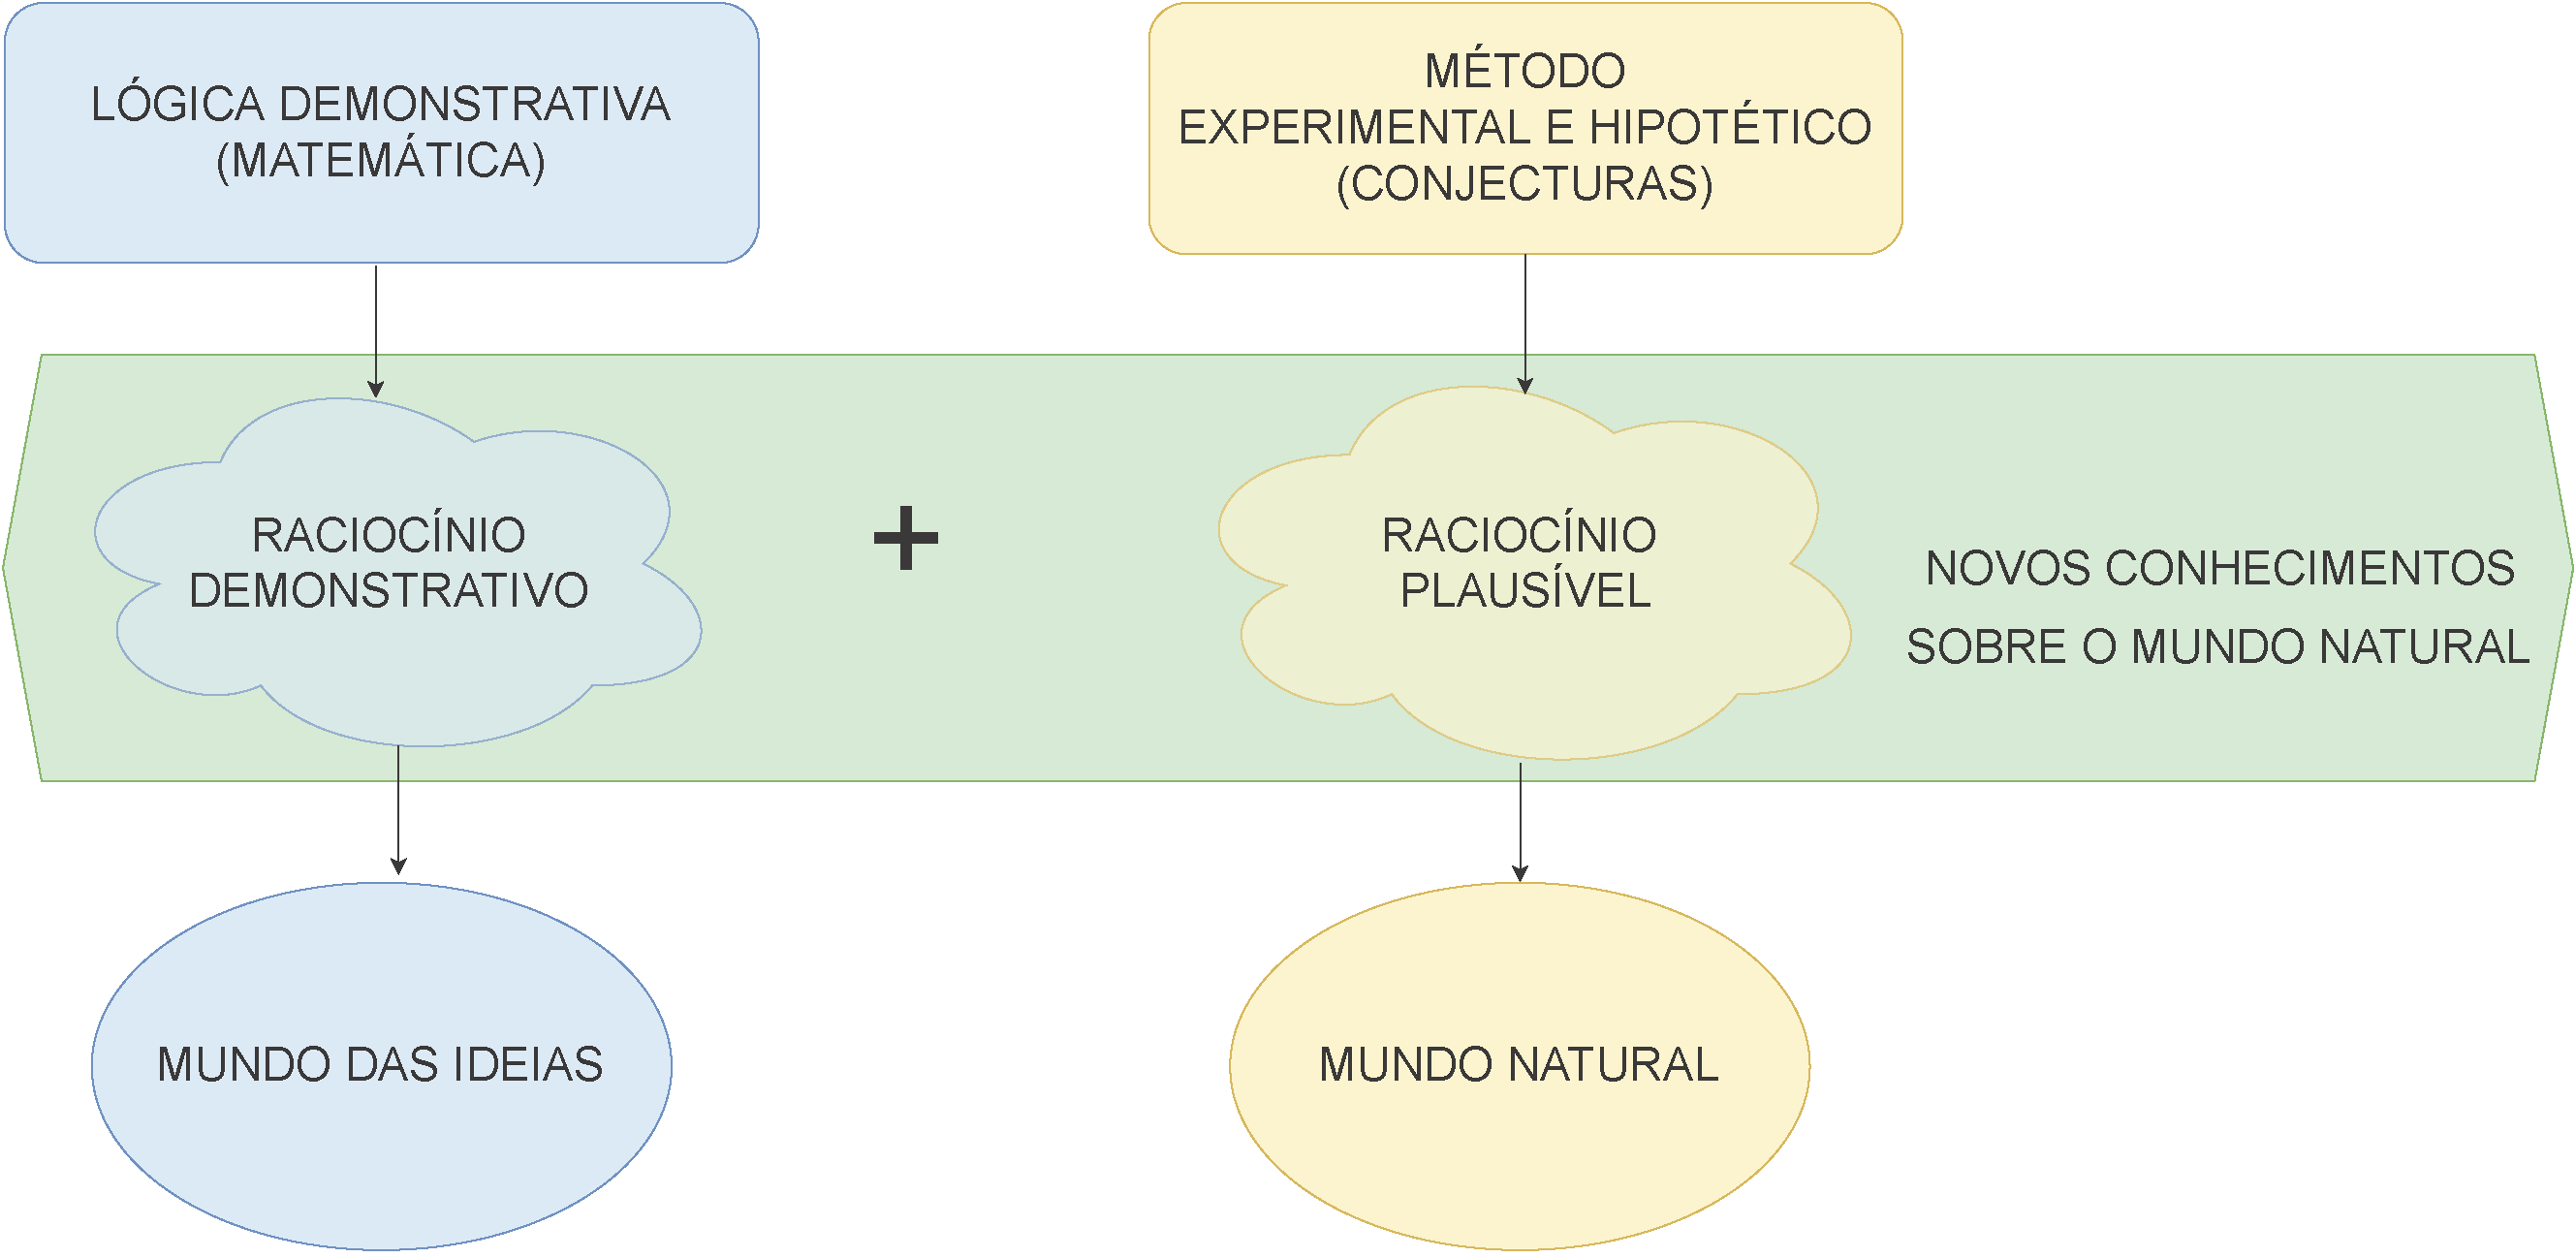
\includegraphics[width=0.8\linewidth]{images11/polya} 

}

\caption{Método demonstrativo e Método experimental hipotético (George Polya, 1954) }\label{fig:unnamed-chunk-3}
\end{figure}

\hfill\break

\emph{Hipotético} porque os cientistas partem de hipóteses sobre os objetos que guiam os experimentos e a avaliação dos resultados e \emph{experimental} porque se baseia em observações e em experimentos, tanto para formular quanto para verificar as teorias.

\hfill\break

O método hipotético experimental pode ser indutivo (fatos \(\to\) lei geral) ou dedutivo (lei geral \(\to\) fatos).

\hfill\break

Isso é observado em qualquer que seja a área do conhecimento:

\hfill\break

\begin{itemize}
\tightlist
\item
  ciências biológicas;\\
\item
  ciências exatas;\\
\item
  ciências agrárias;\\
\item
  ciências humanas;\\
\item
  ciência sociais e outras.
\end{itemize}

\hfill\break

\begin{figure}

{\centering 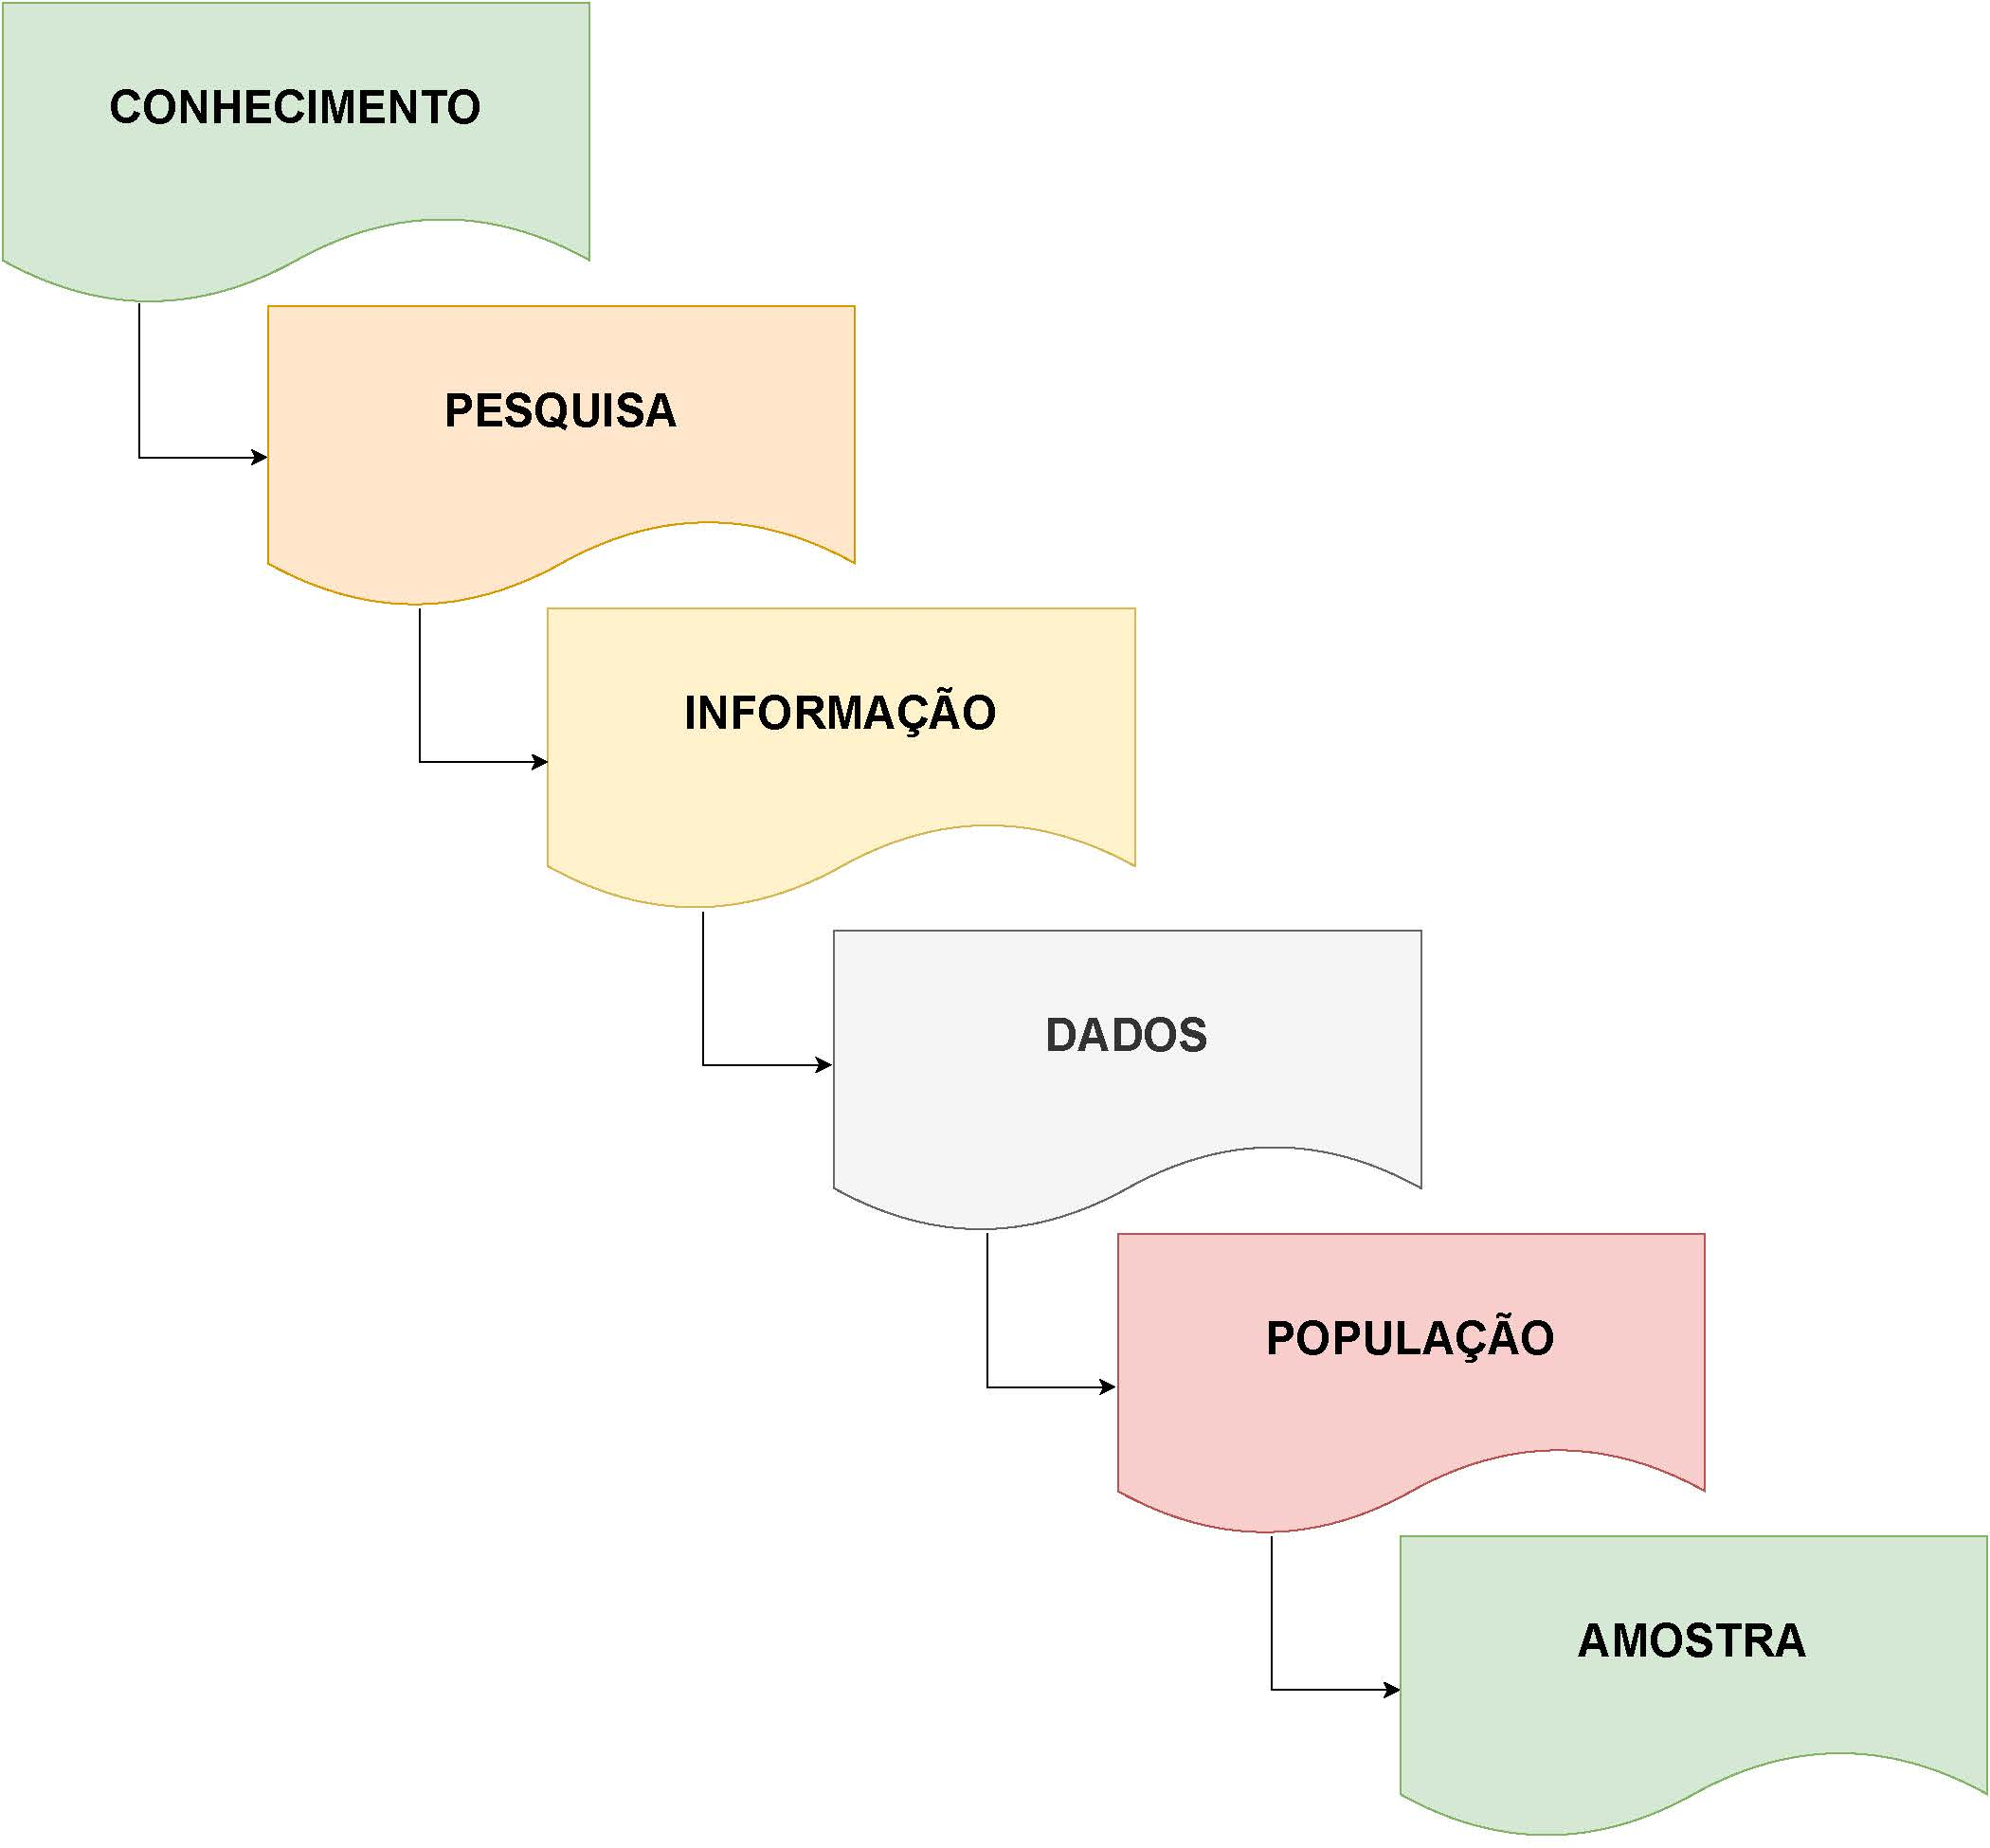
\includegraphics[width=0.8\linewidth]{images1/esquema} 

}

\caption{Representação esquemática do fluxo de infomações da amostra à produção de conhecimento }\label{fig:figProdConhec}
\end{figure}

\hfill\break

Assim, na investigação científica é imposto ao pesquisador formular perguntas que deverão ser apropriadamente respondidas.

\hfill\break

\begin{itemize}
\tightlist
\item
  comparar esses resultados a outros valores; ou,\\
\item
  comparar resultados obtidos pela aplicação de diferentes métodos/ou produtos (valores centrais, variabilidade, proporções) observados em diferentes amostras.
\end{itemize}

\hfill\break

\begin{figure}

{\centering 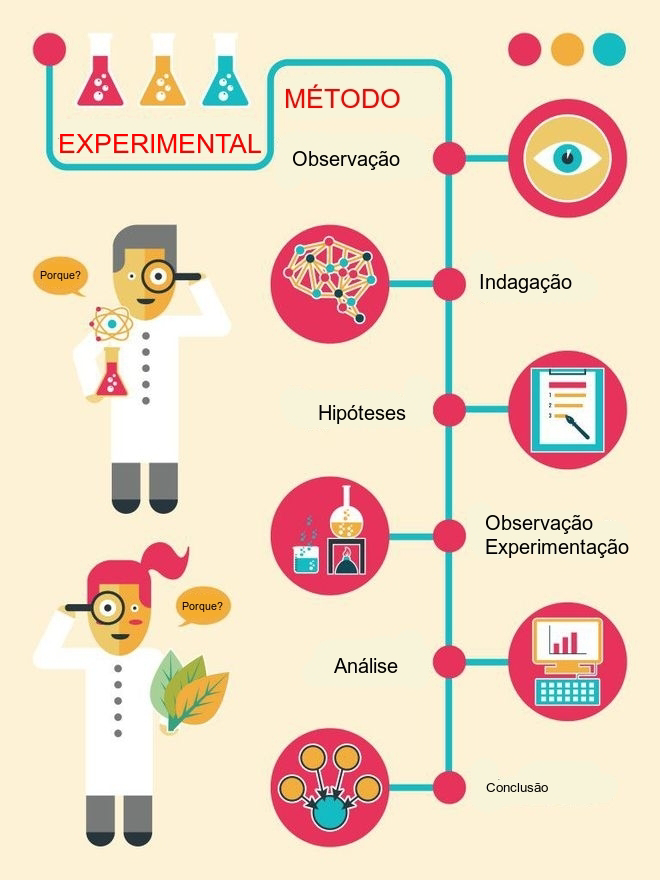
\includegraphics[width=0.8\linewidth]{images1/metodo_experimental} 

}

\caption{Método experimental hipotético}\label{fig:unnamed-chunk-4}
\end{figure}

\hfill\break

Uma hipótese é uma conjectura racional feita após um grande número de observações e experimentos; é uma tese que precisa ser confirmada ou verificada por meio de novas observações e experimentos.

\hfill\break

Uma hipótese estatística é uma suposição feita sobre uma determinada característica de interesse de uma população sob estudo (um parâmetro) que subsiste (perdura, sobrevive, permanece incontestável) até que alguma informação sobre essa população seja estatisticamente significativa para contradizê-la.

\hfill\break

\begin{quote}
``A ciência não consegue provar coisa alguma. Ela pode apenas refutar as coisas'\,' (Karl Popper)
\end{quote}

\hfill\break

\begin{quote}
Uma teoria científica é, portanto, transitória. Uma conjectura temporariamente sustentada que um dia poderá ser refutada e substituída por outra. Conclusões baseadas em raciocínios plausíveis são provisórias, ao contrário daquelas produzidas por raciocínios lógico demonstrativos.
\end{quote}

\hfill\break

\section{Diferentes usos relacionados ao termo, primeiros levantamentos, estudos e publicações (o passado distante)}\label{diferentes-usos-relacionados-ao-termo-primeiros-levantamentos-estudos-e-publicauxe7uxf5es-o-passado-distante}

\hfill\break

O \emph{Domesday Book} \href{http://www.nationalarchives.gov.uk/education/resources/domesday-book/}{(link)}
foi encomendado em dezembro de 1085 por Guilherme, o Conquistador (\emph{King William I}), que invadiu a Inglaterra em 1066.

O primeiro esboço foi concluído em agosto de 1086 e continha registros de 13.418 assentamentos nos condados ingleses ao sul dos rios Ribble e Tees (a fronteira com a Escócia) com informações sobre terras, proprietários, uso da terra, empregados e animais cujo propósito básico era fundamentar a taxação (Figura \ref{fig:figA1}).

\hfill\break

\begin{figure}

{\centering 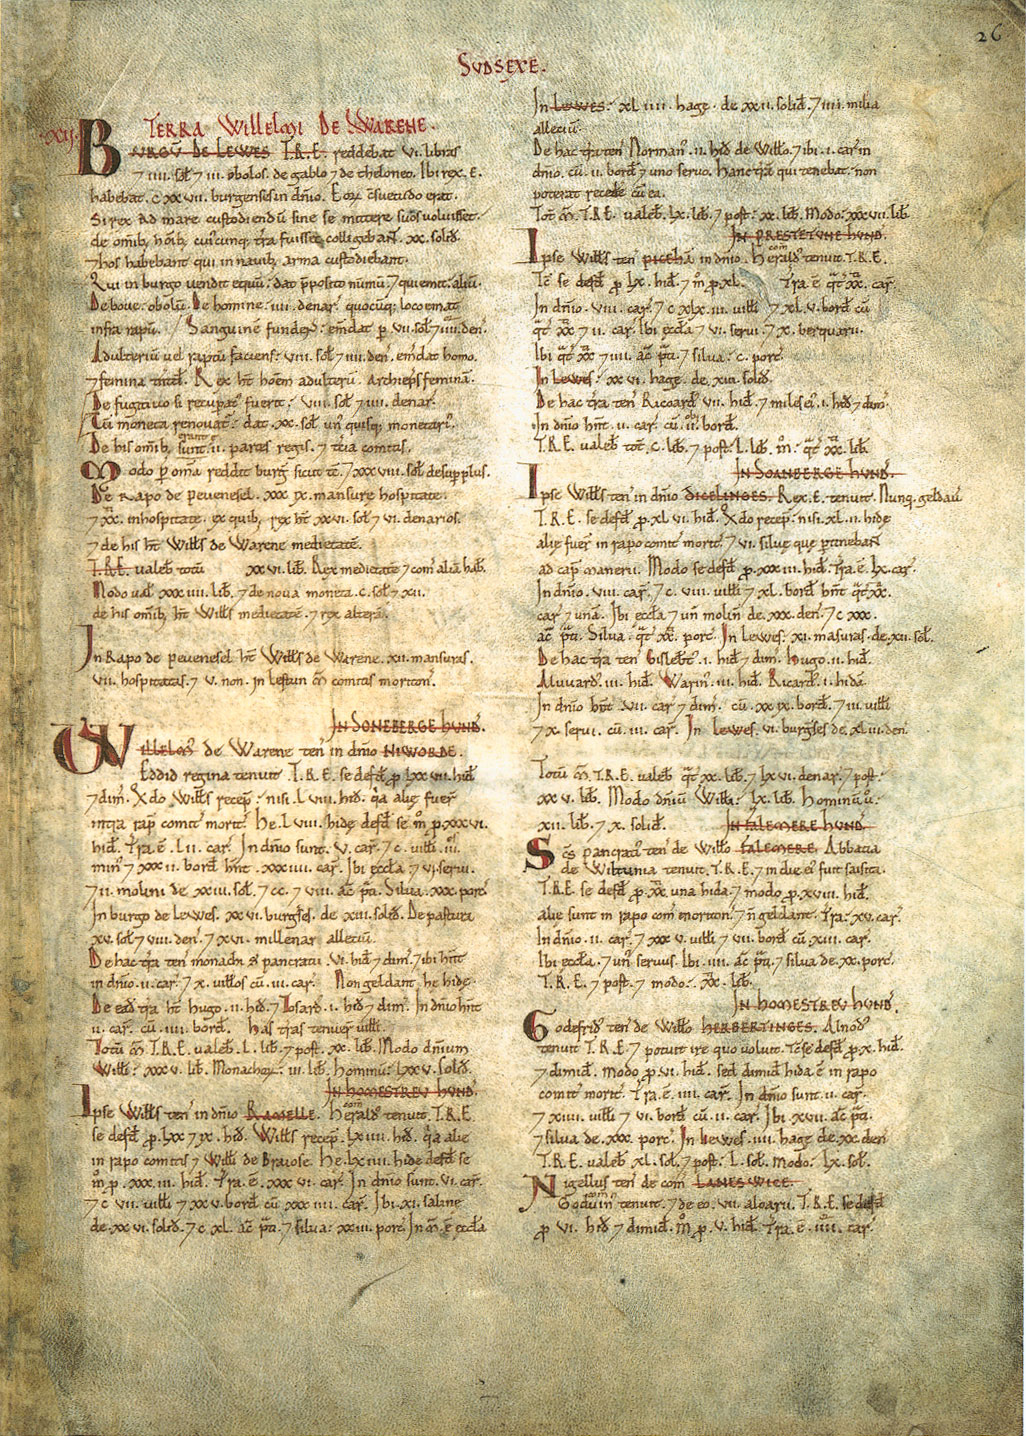
\includegraphics[width=0.75\linewidth]{images1/domesday} 

}

\caption{Domesday Book}\label{fig:figA1}
\end{figure}

\hfill\break

O dramaturgo inglês William Shakespeare usou a palavra \textbf{statists} (estadistas e, portanto, num sentido não relacionado com números ou matemática) no diálogo da Cena II de Hamlet \href{http://shakespeare.mit.edu/hamlet/full.html}{(link)}.

\hfill\break

\begin{quote}
``Hamlet:
Cercado assim por tantas vilanias, mesmo antes de eu poder dizer o prólogo, representava o cérebro.
Sentei-me e escrevi com capricho nova carta. Já pensei, como os nossos estadistas, que é feio escrever bem, tendo insistido, até, em desaprendê-lo; mas, nessa hora muito bom me foi isso. Quererias saber
qual o conteúdo da mensagem?{[}\ldots{]}''
\end{quote}

\hfill\break

Um ponto de partida para a compreensão a ligação entre \emph{estado} e \emph{estatística} é Hermann Conring (1606-1681), professor de filosofia, medicina e política da Universidade de Helmstadt (atual Alemanha), criou um curso de Ciência política em 1660 para funcionários do estado, que descrevia e examinava as questões fundamentais do Estado. Nele a palavra \emph{estatística} (parece ter) passado a ser considerada como uma disciplina autônoma que tinha por objetivo a descrição das coisas do Estado (Figura \ref{fig:figHermann}).

\hfill\break

\begin{figure}

{\centering 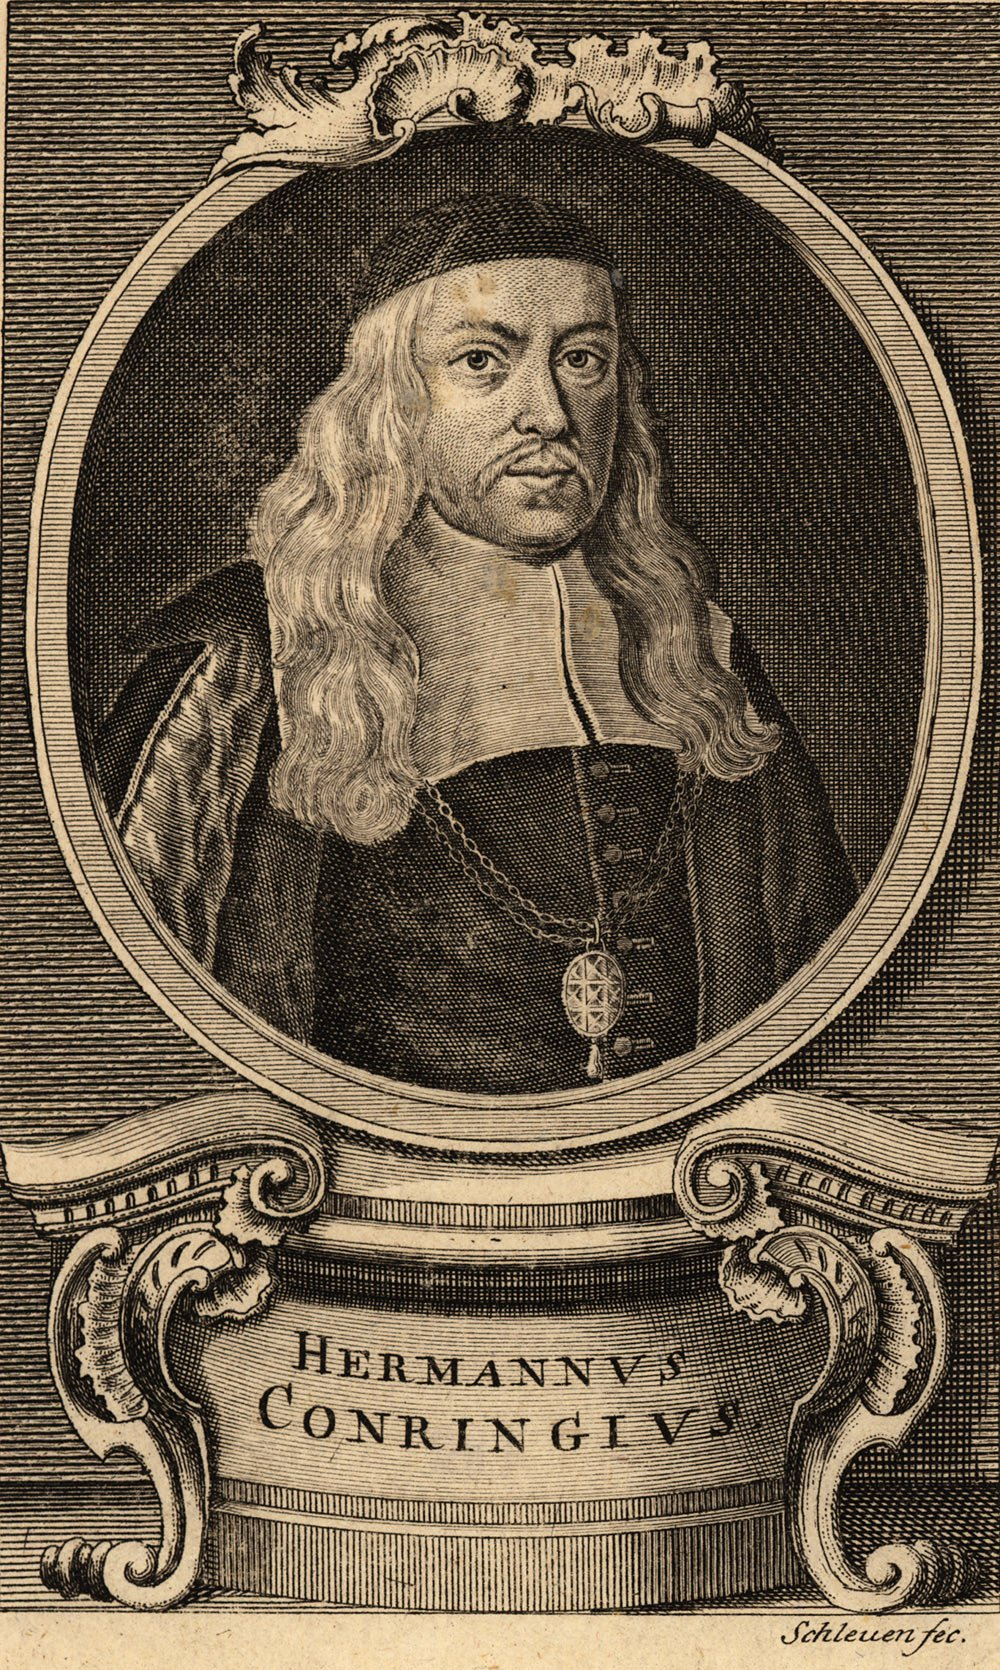
\includegraphics[width=0.75\linewidth]{images1/Hermann_Conring} 

}

\caption{Hermann Conring (1606-1681)}\label{fig:figHermann}
\end{figure}

\hfill\break

\emph{Microscopium Statisticum: quo status imperii Romano-Germanici cum primis extraordinarius, ad vivum repraentatur} (Statistical Microscope: An Analysis of the State, in which the State of the Germanic Roman Empire is vividly represented, above all extraordinary) é um livro cujo título normalmente chama mais atenção do que seu conteúdo: o uso de \emph{statisticum} -- que significa \emph{do estado} -- é reconhecido como um dos primeiros passos em direção ao uso da palavra \emph{estatística} como hoje empregamos (Figura \ref{fig:figMicroscopium}). Foi publicado sob o pseudônimo de Helenus Politanus em 1672.

\hfill\break

\begin{figure}

{\centering 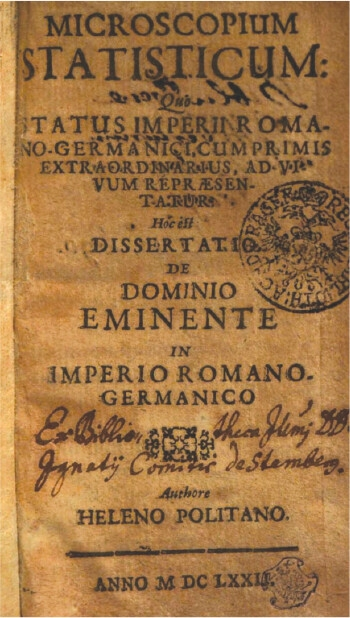
\includegraphics[width=0.75\linewidth]{images1/microscopium} 

}

\caption{Microscopium Statisticum (ed. de 1672)}\label{fig:figMicroscopium}
\end{figure}

\hfill\break

Johan Peter Süßmilch é mais conhecido por seu notável trabalho de 1741 sobre população, conectando o direito natural e a aritmética política. O trabalho de Süssmilch foi amplamente referenciado por Robert Malthus (1798). Ele reconheceu não apenas a ``proporção geométrica'' da fertilidade humana, mas também o efeito de padrões de vida mais elevados sobre o problema populacional (Figura \ref{fig:figPeter}).

\hfill\break

\begin{figure}

{\centering 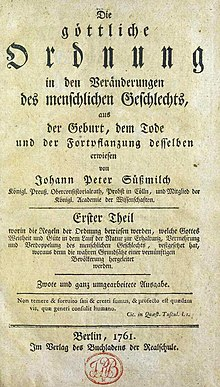
\includegraphics[width=0.75\linewidth]{images1/peter} 

}

\caption{The Divine order in the circumstances of the human sex (1741)}\label{fig:figPeter}
\end{figure}

\hfill\break

Com um sentido não relacionado com números ou matemática, a palavra \textbf{estatística} parece ter sido também proposta no século XVII, pelo historiador e professor alemão (à época Transilvânia) Martin Schmeitzel (1679-1747) da Universidade de Jena e, posteriormente adotada por seu aluno, (igualmente) historiador e jurista Gottfried Achenwall (1719-1772) em 1749, em \emph{Abriß der neuen Staatswissenschaft der vornehmen Europäischen Reiche und Republiken} (Esboço da nova ciência política dos nobres impérios europeus e repúblicas, Figura \ref{fig:figA5}).

\hfill\break

\begin{figure}

{\centering 
\includegraphics[width=0.75\linewidth]{images1/gottfried} 

}

\caption{Abriß der neuen Staatswissenschaft der vornehmen Europäischen Reiche und Republiken (1749)}\label{fig:figA5}
\end{figure}

\hfill\break

Muitos anos depois, William Hooper usou a palavra \textbf{estatística} em sua tradução de \emph{The Elements of Universal Erudition}(Elementos da Erudição Universal) escrita por Jacob Friedrich Freiherr von Bielfeld (1717-1770). Nesse livro, a \emph{estatística} foi definida como a ciência que nos ensina o arranjo político de todos os estados modernos do mundo conhecido (novamente num sentido não associado a números ou matemática, Figura \ref{fig:figA6}).

\hfill\break

\begin{figure}

{\centering 
\includegraphics[width=0.75\linewidth]{images1/hooper} 

}

\caption{The Elements of Universal Erudition  (1771)}\label{fig:figA6}
\end{figure}

\hfill\break

Na Inglaterra a palavra estatística estava mais associada ao estudo de dados numéricos como modo de se obter \emph{insights} sobre questões sociais e demográficas no país. Dois pioneiros nessa linha foram William Petty e John Graunt. Em 1687 o economista e filósofo inglês William Petty (1623-1687) publicou \emph{Several Essays on Political Arithmetic} (Vários ensaios sobre aritmética política), sugerindo ao governo inglês a criação de um departamento para registro de \emph{estatísticas} vitais (Figura \ref{fig:figA3}).

\hfill\break

\begin{figure}

{\centering 
\includegraphics[width=0.75\linewidth]{images1/petty} 

}

\caption{Several Essays in Political Arithmetick (ed. de 1699)}\label{fig:figA3}
\end{figure}

\hfill\break

O negociante inglês John Graunt (1620-1674) substituiu a crença pela evidência em \emph{Natural and Political Observations Mentioned in a Following Index and Made upon the Bills of Mortality} (Observações naturais e políticas feitas sobre as notas de mortalidade).

\hfill\break

Nesse trabalho, realizado com dados coletados das paróquias de Londres entre 1604 e 1660, Graunt tirou as seguintes conclusões: que havia maior nascimento de crianças do sexo masculino, mas havia distribuição aproximadamente igual de ambos os sexos na população geral; alta mortalidade nos primeiros anos de vida; maior mortalidade nas zonas urbanas em relação às zonas rurais (Figura \ref{fig:figA2}).

\hfill\break

\begin{figure}

{\centering 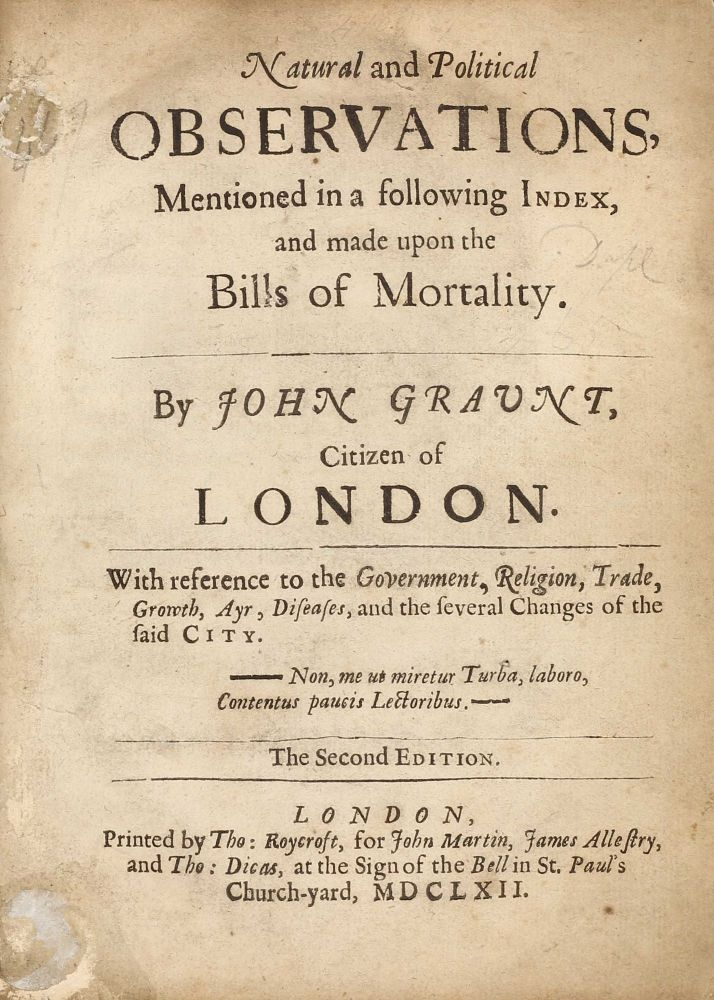
\includegraphics[width=0.75\linewidth]{images1/graunt} 

}

\caption{Natural and Political Observations Mentioned in a Following Index and Made upon the Bills of Mortality (ed. de 1662)}\label{fig:figA2}
\end{figure}

\hfill\break

O matemático e astrônomo inglês Edmond Halley (1656-1742) construiu em 1693, baseado em dados coletados na cidade (à época) alemã de Bresláu, uma \emph{Life Table} (Tábua de sobrevivência), um estudo que analisa as probabilidades de sobrevivência e morte em relação à idade (Figura \ref{fig:figA4}).

\hfill\break

\begin{figure}

{\centering 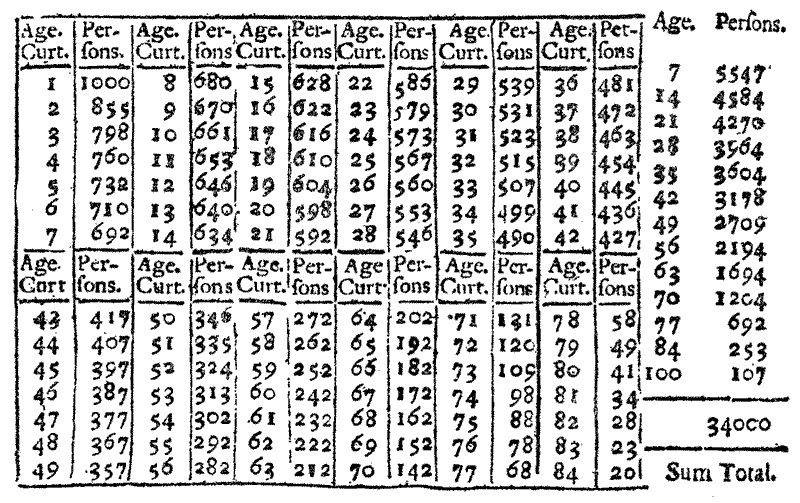
\includegraphics[width=0.75\linewidth]{images1/halley} 

}

\caption{Halley’s life table (1693)}\label{fig:figA4}
\end{figure}

\hfill\break

O jurista e político escocês John Sinclair propôs que se realizasse uma detalhada pesquisa em 938 paróquias para elucidar a história natural e política de seu país ( \emph{Statistics Accounts} ). Essa pesquisa fazia parte de um projeto muito mais ousado: \emph{The Pyramid of Statistical Enquiry} (A Pirâmide da Pesquisa Estatística, Figura \ref{fig:figA7}).

\hfill\break

\begin{figure}

{\centering 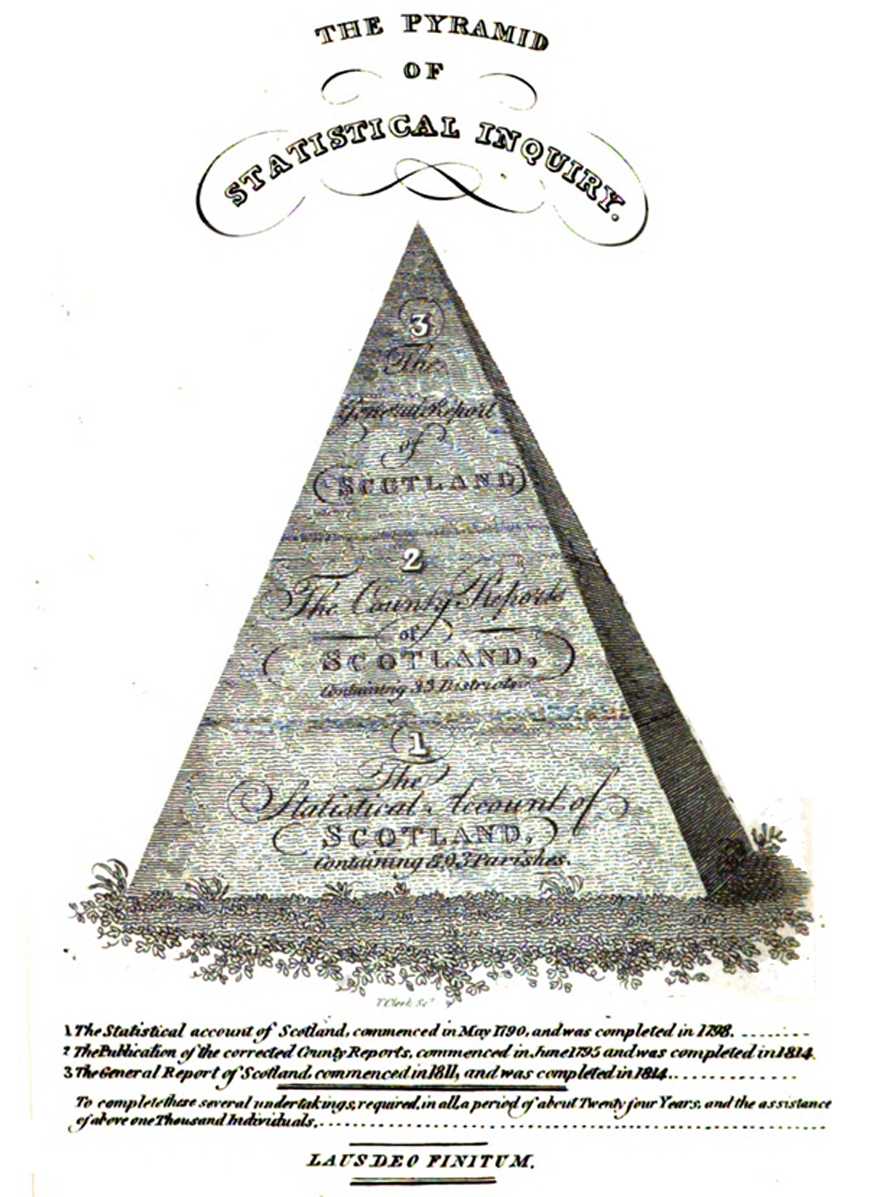
\includegraphics[width=0.75\linewidth]{images1/sinclair} 

}

\caption{The Pyramid of Statistical Enquiry  (1814)}\label{fig:figA7}
\end{figure}

\hfill\break

Outro trabalho com vertente demográfica foi o de Sébastien Le Prestre, Marquês de Vauban (1633--
1707), intitulado \emph{Méthode générale et facile pour faire le dénombrement des peuples}, detakhado num livro de 1686 (Figura \ref{fig:figvauban}).

\hfill\break

\begin{figure}

{\centering 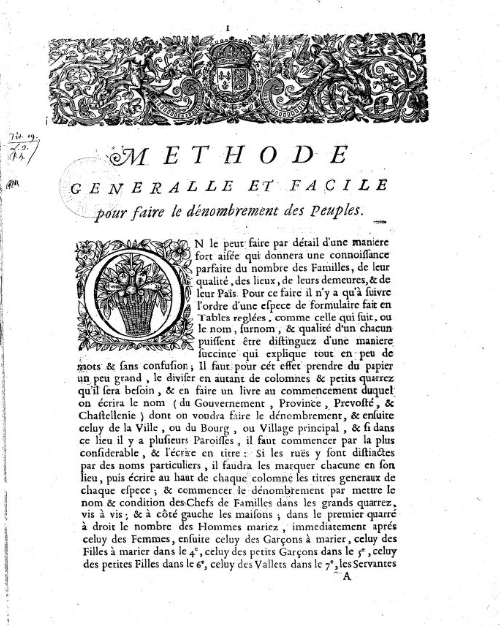
\includegraphics[width=0.75\linewidth]{images1/vauban} 

}

\caption{Méthode générale et facile pour faire le dénombrement des peuples (1686)}\label{fig:figvauban}
\end{figure}

\hfill\break

O médico inglês (considerado por alguns como o ``pai'' da epidemiologia moderna) John Snow (1813-1858) estudou a dispersão espacial dos casos de cólera em Londres e concluiu que sua causa residia na contaminação da água consumida (poço localizado na \emph{Broad Street}, no distrito do \emph{Soho}): \emph{Report to the Cholera Outbreak in the Parish of St.~James, Westminster during the Autumn of 1854} (Relatório sobre o surto de cólera na paróquia de St.~James, Westminster durante o outono de 1854, Figura \ref{fig:figA8}).

\hfill\break

\begin{figure}

{\centering 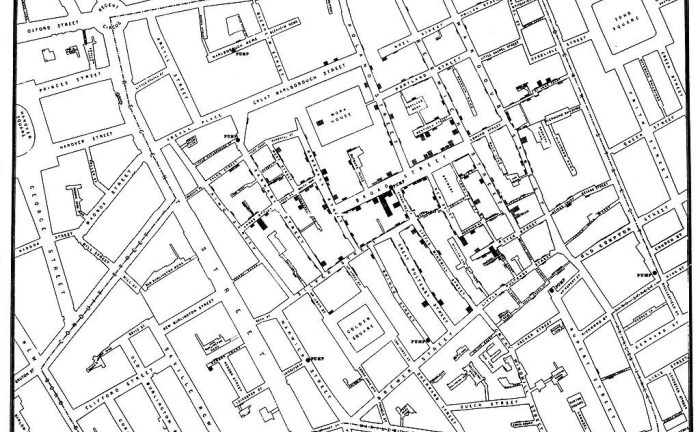
\includegraphics[width=0.75\linewidth]{images1/london-1854-snow} 

}

\caption{Mapa dos casos de cólera (1854)}\label{fig:figA8}
\end{figure}

\section{Visualização de dados \& Estudos e primeiras publicações}\label{visualizauxe7uxe3o-de-dados-estudos-e-primeiras-publicauxe7uxf5es}

\hfill\break

O teólogo e filósofo inglês Joseph Priestley (1733-1804) introduziu como inovação os primeiros gráficos com linha temporal, em que barras individuais eram usadas para visualizar o tempo de vida de uma pessoa e o todo pode ser usado para comparar a expectativa de vida de várias pessoas (Figura \ref{fig:figA9}).

\hfill\break

\begin{figure}

{\centering 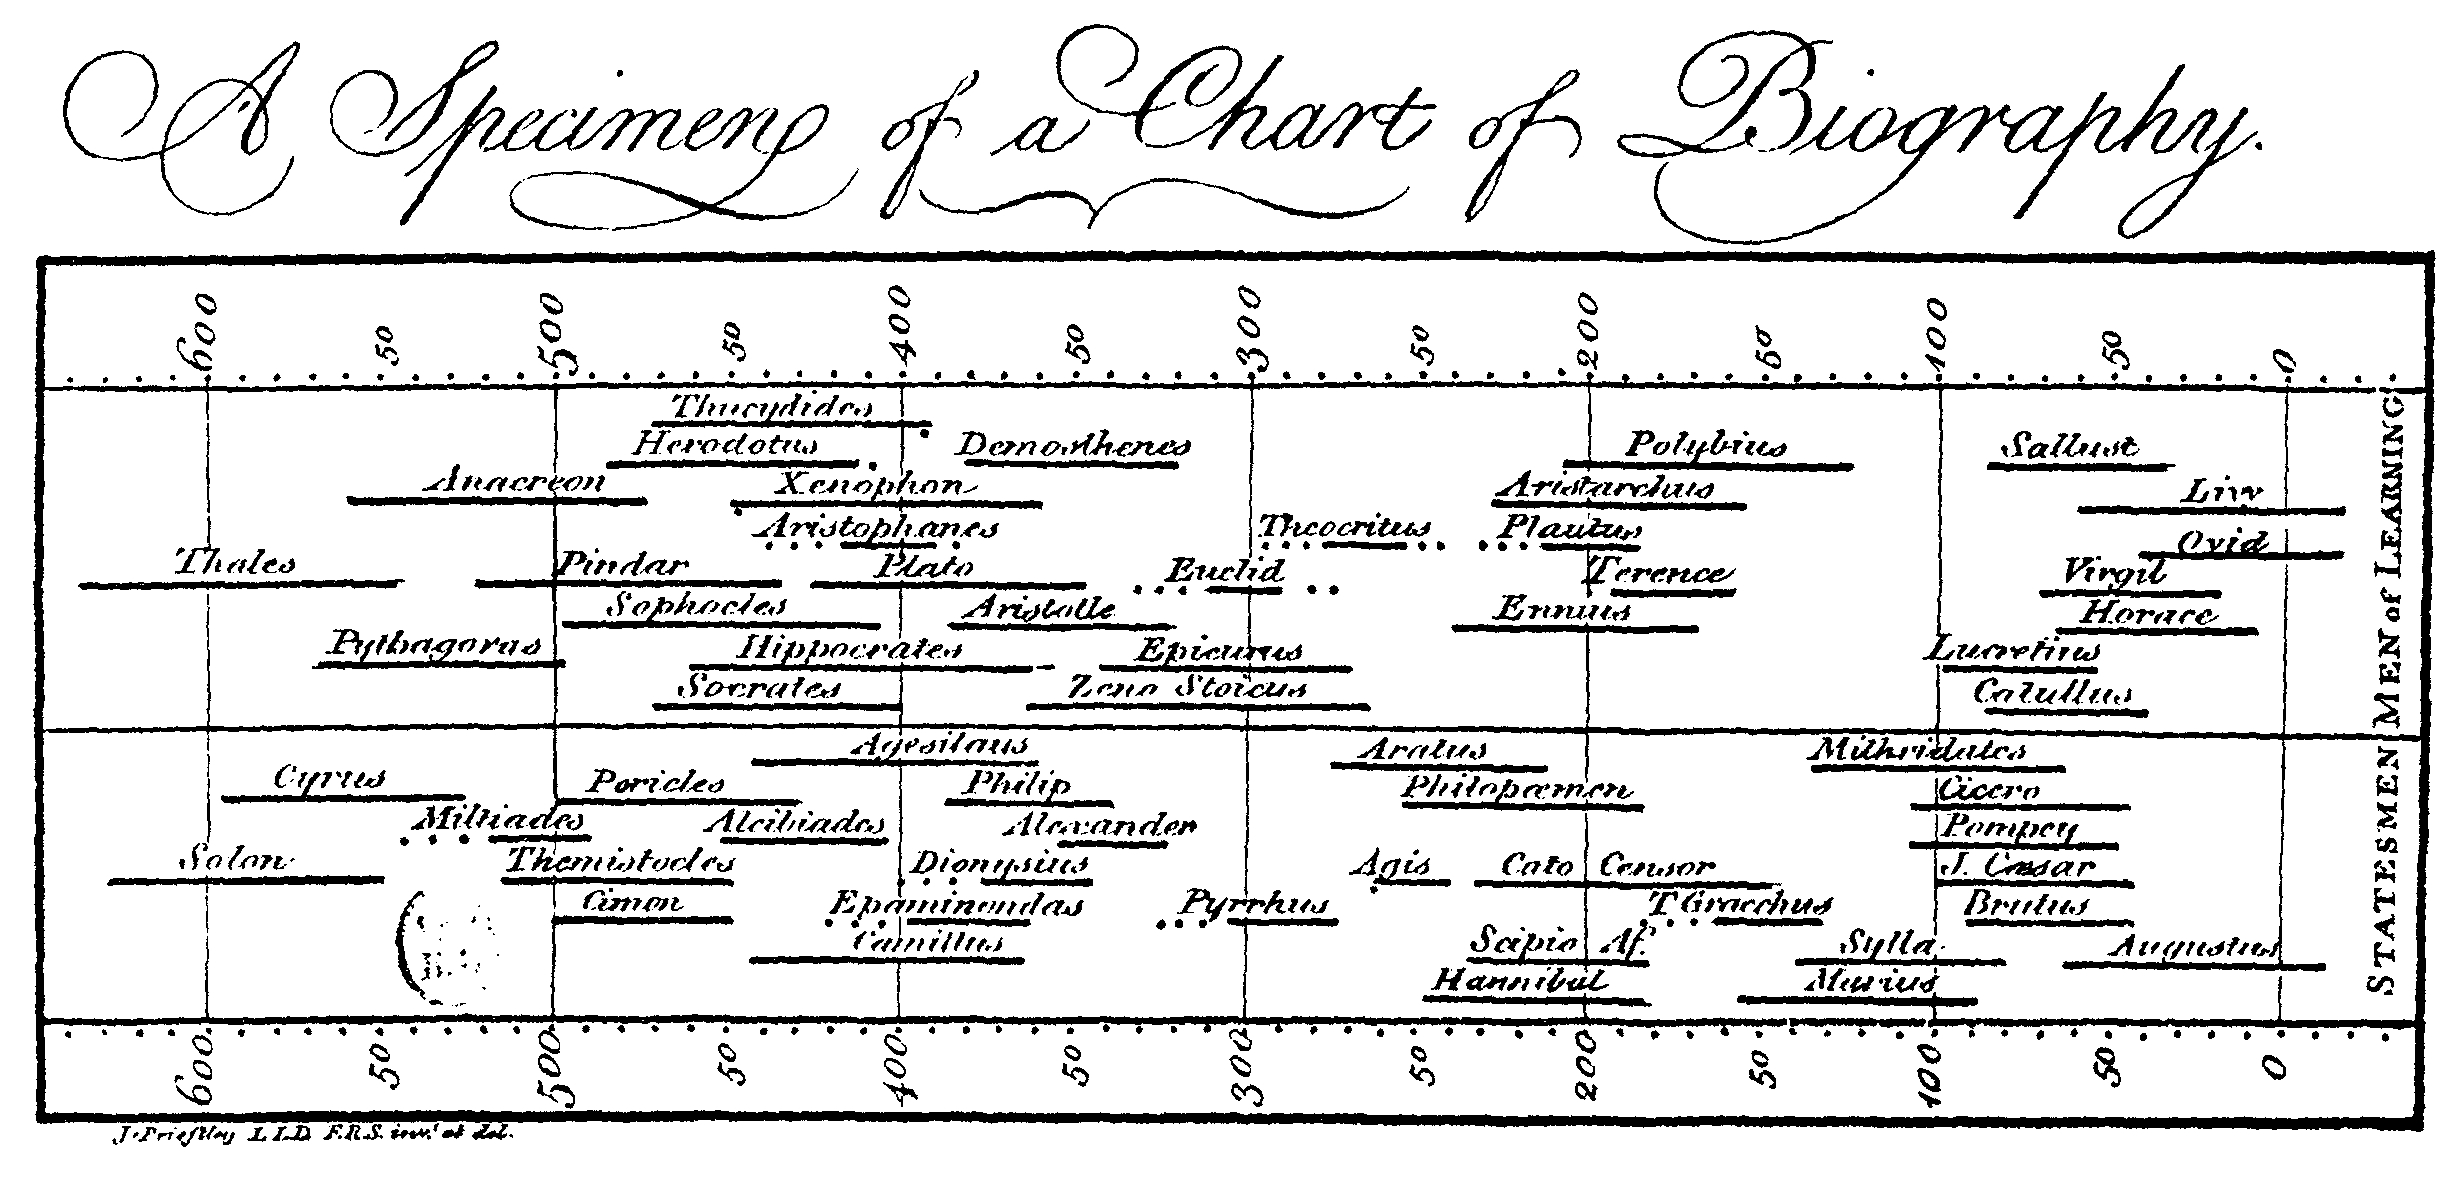
\includegraphics[width=0.75\linewidth]{images1/priestley-timechart-1765} 

}

\caption{Expectativa de vida de diversas pessoas (1765)}\label{fig:figA9}
\end{figure}

\hfill\break

O engenheiro e economista escocês William Playfair (1759-1823) é considerado comumente como fundador dos métodos gráficos para apresentação de estatísticas. Playfair concebeu vários tipos de diagramas para visualização de dados:

\begin{itemize}
\tightlist
\item
  em 1786, o gráfico de barras (Figura \ref{fig:figA10}); e,
\item
  em 1801, o gráfico de setores (Figura \ref{fig:figA11}).
\end{itemize}

\hfill\break

\begin{figure}

{\centering 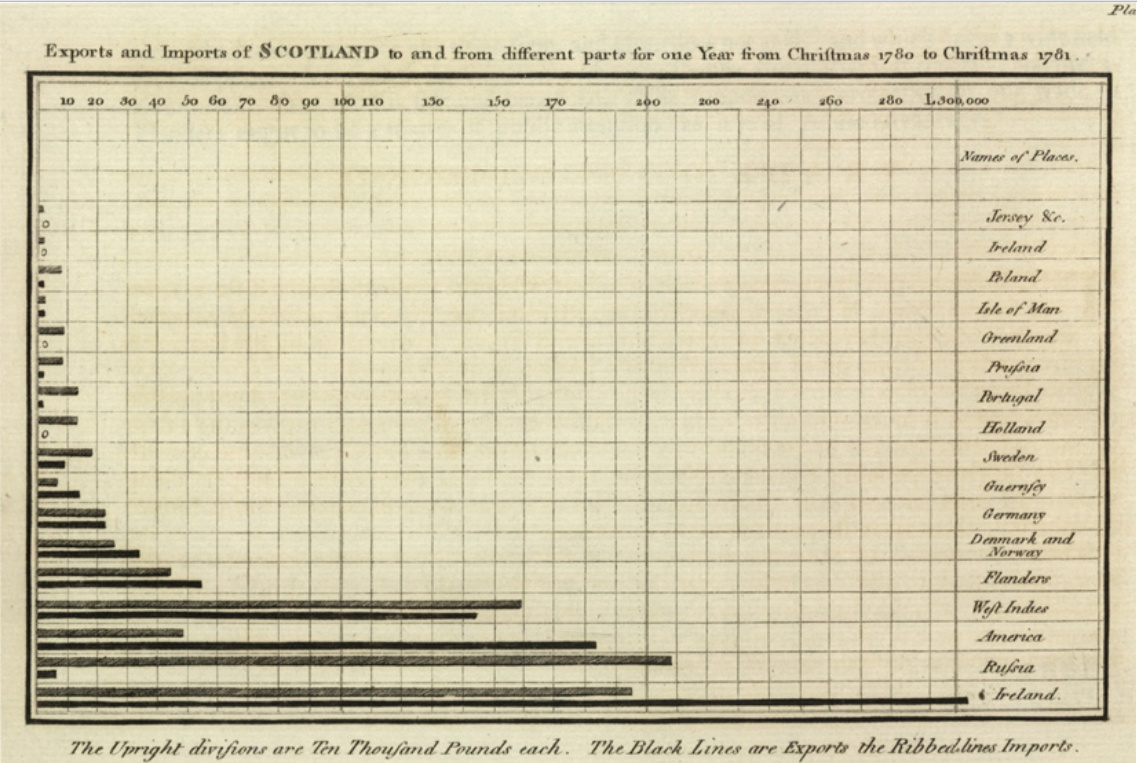
\includegraphics[width=0.75\linewidth]{images1/playfair-barchart-1786} 

}

\caption{Commercial and Political Atlas (Atlas Comercial e Político de 1786): cada barra representa as exportações e importações da Escócia para 17 países em 1781}\label{fig:figA10}
\end{figure}

\hfill\break

\begin{figure}

{\centering 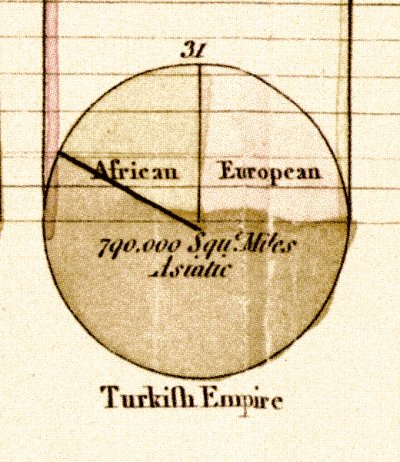
\includegraphics[width=0.75\linewidth]{images1/playfair-piechart-1801} 

}

\caption{Statistical Breviary (Breviário Estatístico de 1801): proporção da extensão do Império Turco em diferentes regiões do mundo: Asia, Europa e África, antes de 1789}\label{fig:figA11}
\end{figure}

\hfill\break

A enfermeira inglesa Florence Nightingale (1820-1910) conduziu um trabalho pioneiro ao chegar no hospital militar britânico na Turquia em 1856, estabelecendo uma ordem e um método muito necessários aos registros médicos estatísticos e que indicaram serem as precárias práticas sanitárias o culpado da alta mortalidade \href{https://www.york.ac.uk/depts/maths/histstat/small.htm}{(link)} , Figuras \ref{fig:figA12} e \ref{fig:figA13}.

\hfill\break

\begin{figure}

{\centering 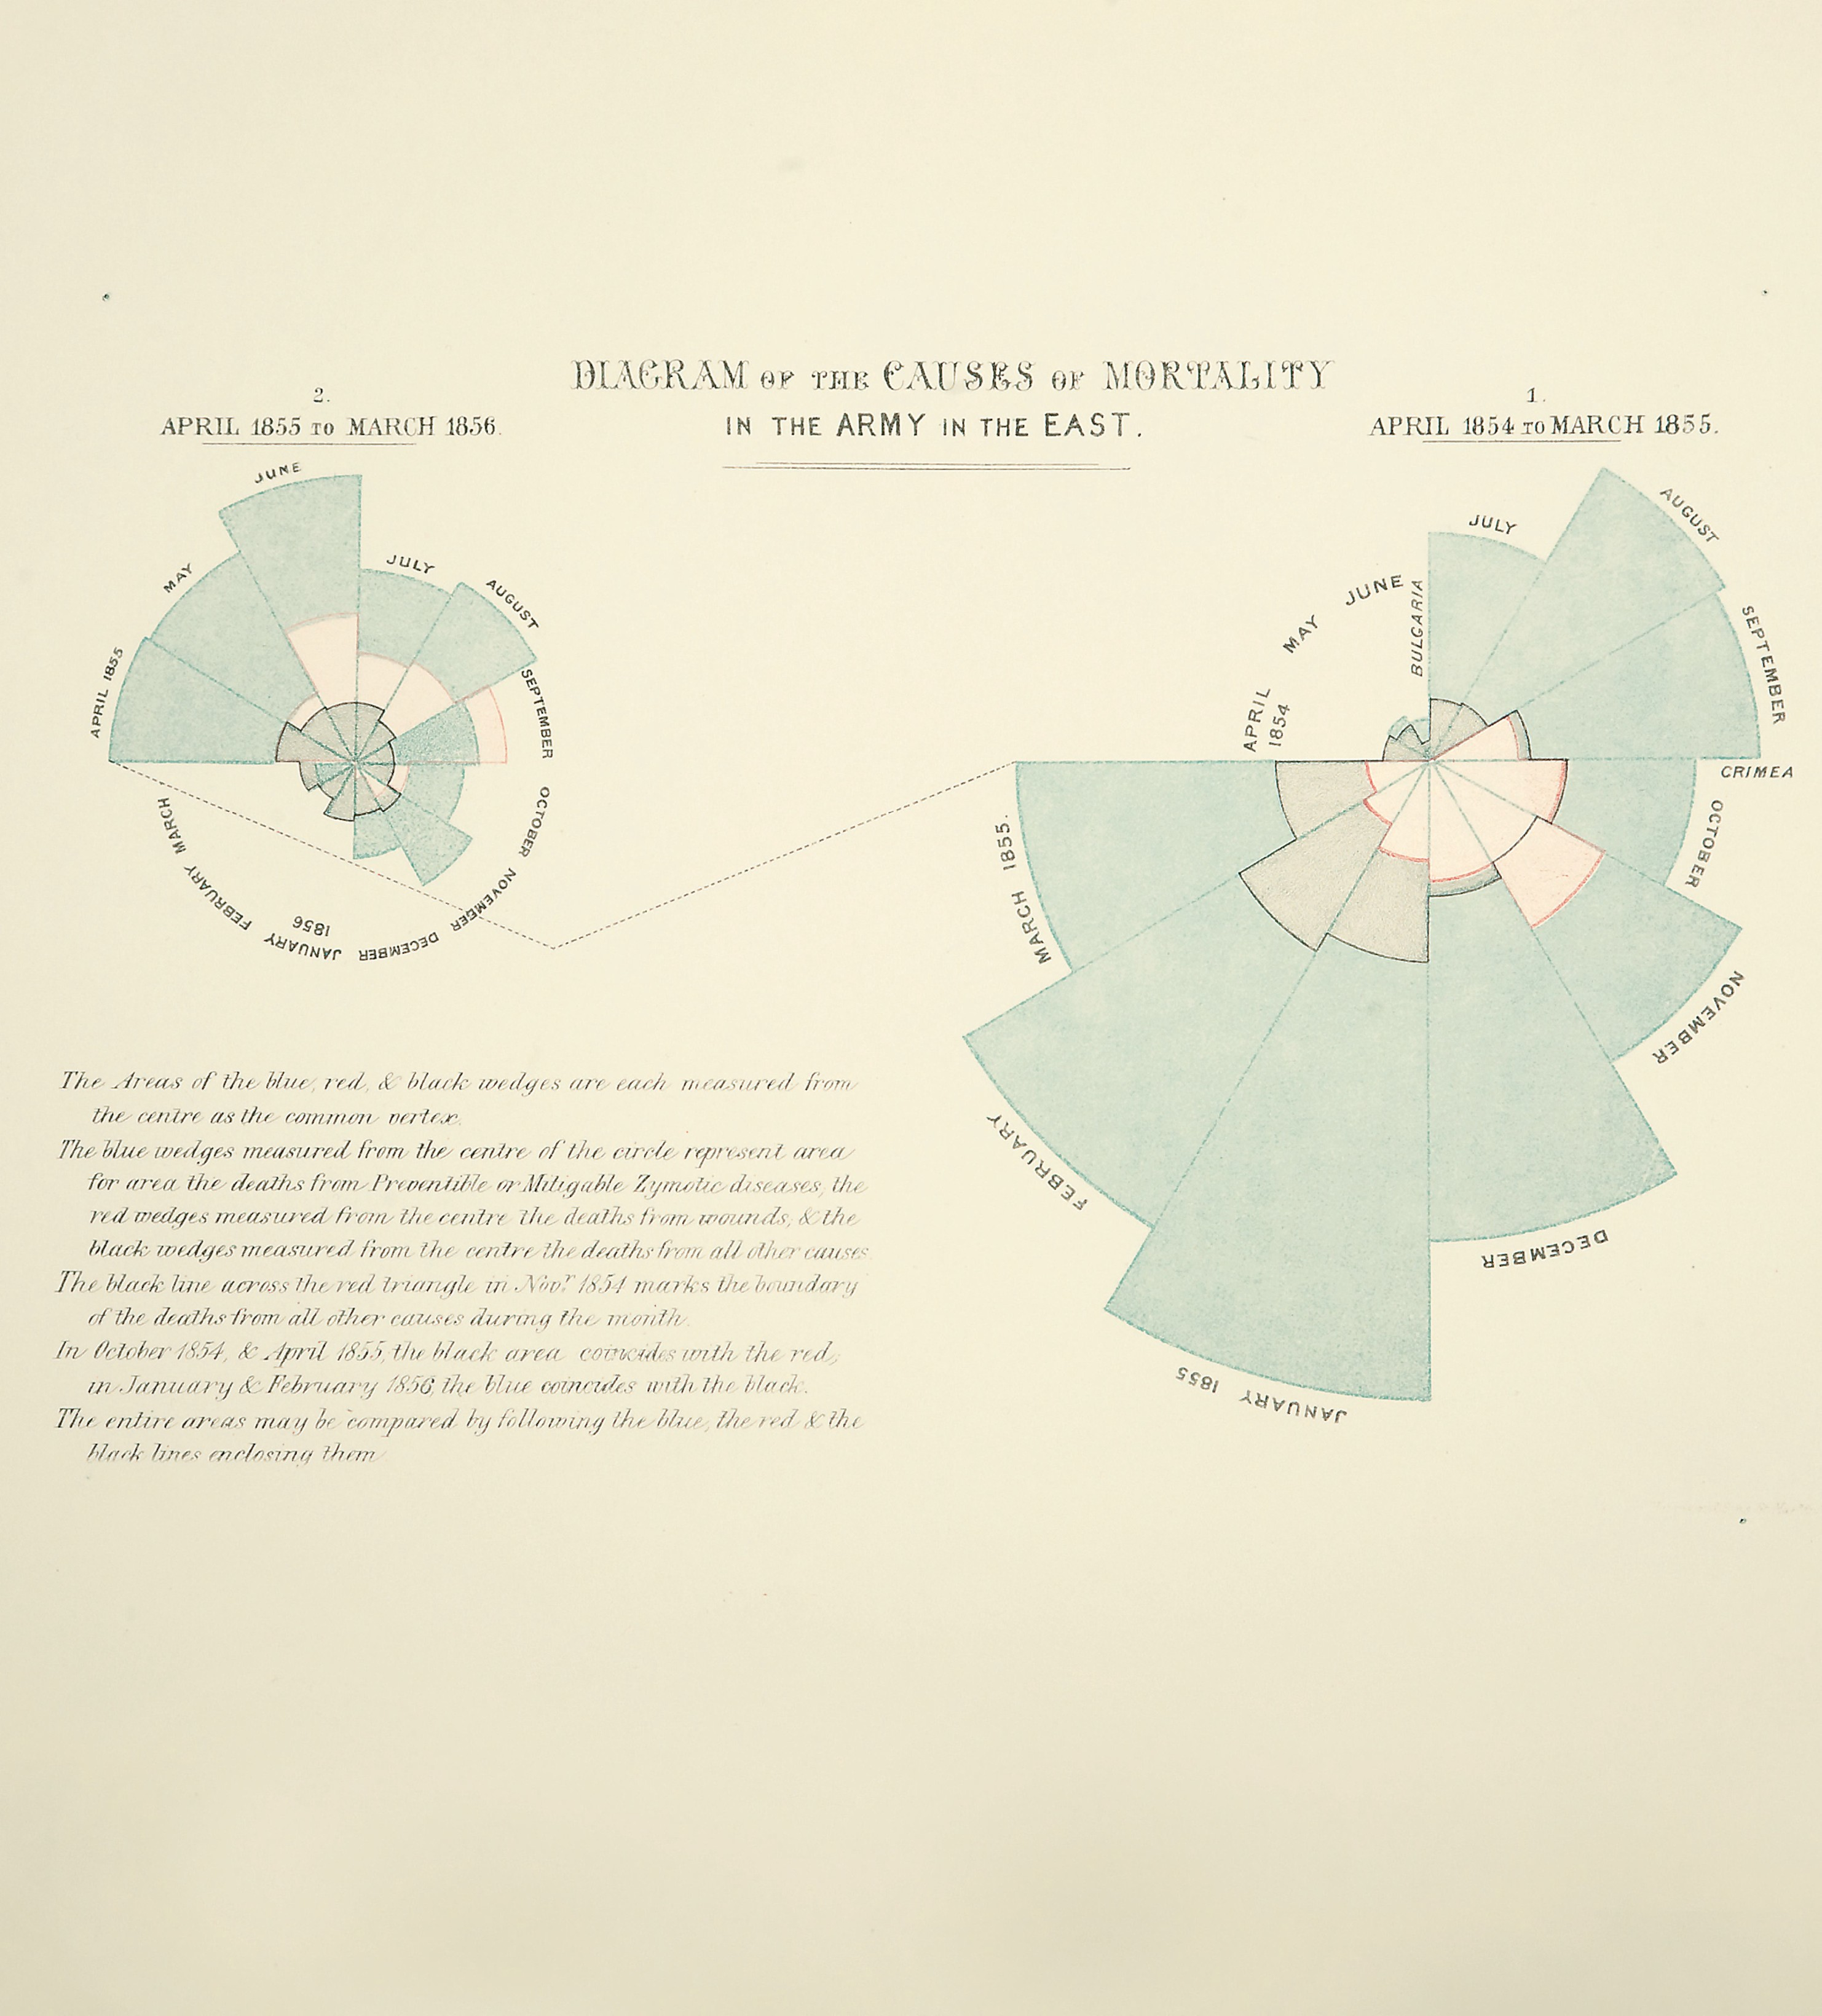
\includegraphics[width=0.75\linewidth]{images1/florence-rose-diagram} 

}

\caption{Esse diagrama (coxcomb) feito durante a Guerra da Crimeia foi dividido igualmente em 12 setores, representando os meses do ano, com a área sombreada do setor  de cada mês proporcional à taxa de mortalidade naquele mês. Seu sombreamento com código de cores indicava a causa da morte em cada área do diagrama}\label{fig:figA12}
\end{figure}

\hfill\break

\begin{figure}

{\centering 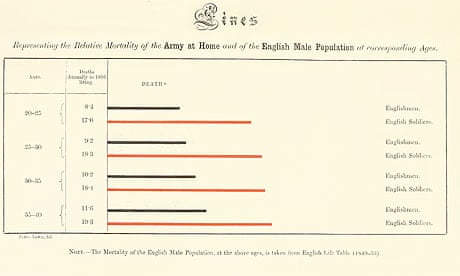
\includegraphics[width=0.75\linewidth]{images1/florence-barr} 

}

\caption{Gráfico de barras de Florence Nightingale mostrando as diferenças de mortalidade entre soldados britânicos e a população masculina inglesa geral (civis)}\label{fig:figA13}
\end{figure}

\hfill\break

\section{Pesquisadores cuja contribuição foi fundamental na área}\label{pesquisadores-cuja-contribuiuxe7uxe3o-foi-fundamental-na-uxe1rea}

\hfill\break

Uma breve biografia de cada um dos pesquisadores a seguir relacionados pode ser obtida em: \href{http://www-history.mcs.st-andrews.ac.uk/BiogIndex.html}{(link)}.

\hfill\break

\begin{itemize}
\tightlist
\item
  Niccolò Fontana Tartaglia (Veneza à época, hoje Itália: 1499-1557)
\item
  Girolamo Cardano (Pávia à época, hoje Itália: 1501-1576)
\item
  Galileu Galilei (Florença à época, hoje Itália: 1564-1642)
\item
  Pierre de Fermat (França: 1607-1665)
\item
  Blaise Pascal (França: 1623-1662)
\item
  Jakob Bernoulli (Suíça: 1655-1705)
\item
  Abrahan de Moivre (França: 1667-1754)
\item
  Thomas Bayes (Inglaterra: 1702-1761)
\item
  Pierre-Simon Laplace (França: 1749-1827)
\item
  Johann Carl Friedrich Gauss (Alemanha: 1777-1856)
\item
  Lambert Adolphe Jacques Quételet (França à época, hoje Bélgica: 1796-1874)
\item
  Pafnuti Lvovitch Chebyshev (Rússia: 1821-1894)
\item
  Francis Galton (Inglaterra: 1822-1911)
\item
  Wilhelm Lexis (Alemanha: 1837-1914)
\item
  Thorvald Nicolai Thiele (Dinamarca: 1838-1910)
\item
  Friedrich Robert Helmert (Saxônia: 1843-1917)
\item
  Francis Ysidro Edgeworth (Inglaterra: 1845-1926)
\item
  James Douglas Hamilton Dickson (Escócia: 1849-1931)
\item
  Andrei Andreyevich Markov (Rússia: 1856-1922)
\item
  Aleksandr Mikhailovich Lyapunov (Rússia: 1857-1918)
\item
  Walter Frank Raphael Weldon (Inglaterra: 1860-1906)
\item
  Karl Pearson (Inglaterra: 1857-1936)
\item
  William Seally Gosset (Inglaterra: 1876-1937)
\item
  Ronald Aylmer Fisher (Inglaterra: 1890-1962)
\item
  Andrei Nikolaevich Kolmogorov (Rússia: 1903-1987)
\end{itemize}

\section{Revista Biometrika}\label{revista-biometrika}

\hfill\break

Karl Pearson (1857-1936) é amplamente considerado o fundador da disciplina moderna de \textbf{estatística}, e também é famoso como um filósofo da ciência, como escritor sobre o darwinismo social e como um dos principais impulsionadores para instalar a eugenia como a ciência social chave.

\hfill\break

\begin{quote}
``Pretende-se que a \emph{Biometrika} sirva como um meio não apenas de coletar ou publicar, sob um título, dados biológicos de um tipo não coletados sistematicamente ou publicados em outro lugar em qualquer outro periódico, mas também de disseminar um conhecimento de tal teoria estatística para o seu tratamento científico{[}\ldots{]}''
\end{quote}

\hfill\break

Em outubro de 1901 foi fundada a \emph{Biometrika, the Journal for the Statistical Study of Biological Problems} (Biometrika, o Jornal para o Estudo Estatístico de Problemas Biológicos) com o propósito de promover a análise estatística de fenômenos biológicos, isto é, a matematização da biologia.

\hfill\break

Os fundadores da \emph{Biometrika} foram \emph{Sir} Francis Galton (primo de Charles Darwin), Walter Frank Raphael Weldon e Karl Pearson. A maior parte do trabalho foi feita por Pearson e Weldon, este último focando na edição do conteúdo (ou seja, o aspecto biológico) e o primeiro nos detalhes, incluindo correções de prova. Galton e o eugenista americano Charles Davenport atuaram, respectivamente, como consultor e editor.

\hfill\break

Alguns dos tópicos abordados na revista incluem criminologia, botânica, zoologia, epidemiologia e outros aspectos da saúde humana. Na década de 1930, o caráter da \emph{Biometrika} mudou, e ``representou a vanguarda internacional da pesquisa em métodos estatísticos e sua aplicação na ciência e tecnologia'\,', ao invés de focar a hereditariedade.

\hfill\break

\emph{Sir} Francis Galton, que serviu como editor da primeira edição (1901), escreveu a Introdução, que incluiu uma declaração de propósito para a revista\\
\href{https://academic.oup.com/biomet/article-abstract/1/1/1/192192?redirectedFrom=fulltext}{(link)}.

\hfill\break

\section{Eugenia}\label{eugenia}

\hfill\break

Em 16 de maio de 1883 \emph{Sir} Francis Galton cunhou o termo \emph{eugenia}, posteriormente descrevendo-o como ``o estudo das agências sob controle social que podem melhorar ou reparar as qualidades raciais das gerações futuras, seja fisicamente ou mentalmente''.

\hfill\break

Galton detalha o conceito em seu livro \emph{Inquiries into Human Faculty and its Development}, e recomenda que indivíduos de famílias altamente classificadas em seu sistema de mérito sejam encorajados a se casar cedo e receber incentivos para ter filhos. Ele também condenou os casamentos tardios dentro desse mesmo grupo como ``disgênicos'' ou desvantajosos para a espécie humana.

\hfill\break

A palavra \emph{eugenia} foi extraída da palavra grega \emph{eu}, que significa bem, e \emph{genos}, que significa prole. Juntos, significaria \emph{bem-nascido}.

\hfill\break

Este livro caiu em domínio público e pode ser lido na íntegra online. A caracterização original de eugenia de Galton pode ser encontrada na página 17 desta edição de domínio público (Parte 1 do pdf):

\hfill\break

\begin{quote}
``uma breve palavra para expressar a ciência de melhorar o rebanho, que não está de modo algum confinado a questões de acasalamento criterioso, mas que, especialmente no caso do homem, toma conhecimento de todas as influências que tendem, mesmo que em grau remoto, a dar ao raças ou linhagens de sangue mais adequadas uma melhor chance de prevalecer rapidamente sobre os menos adequados do que teriam de outra forma {[}\ldots{]}''(Galton, 1883, p.17)
\end{quote}

\hfill\break

Mais recentemente, alguns grupos sociais viram no trabalho e opiniões de Fisher endossos ao colonialismo, à supremacia branca e à eugenia (como hoje interpretada).

\hfill\break

Outros grupos, todavia, afirmam que Fisher não era racista nem eugenista, embora ele achasse que havia diferenças comportamentais e de inteligência entre os grupos humanos.

\hfill\break

\begin{figure}

{\centering 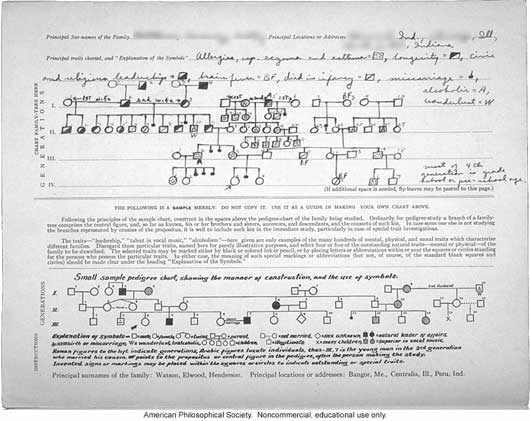
\includegraphics[width=0.75\linewidth]{images1/chart_pedigree_allergy2} 

}

\caption{Gráfico de linhagens para alergias}\label{fig:figA14}
\end{figure}

\hfill\break

\begin{figure}

{\centering 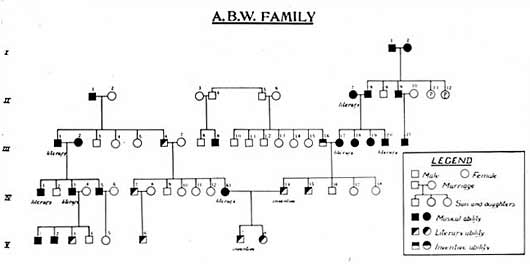
\includegraphics[width=0.75\linewidth]{images1/chart_pedigree_music2 (1)} 

}

\caption{Gráfico de linhagens para aptidão musical}\label{fig:figA15}
\end{figure}

\hfill\break

\begin{figure}

{\centering 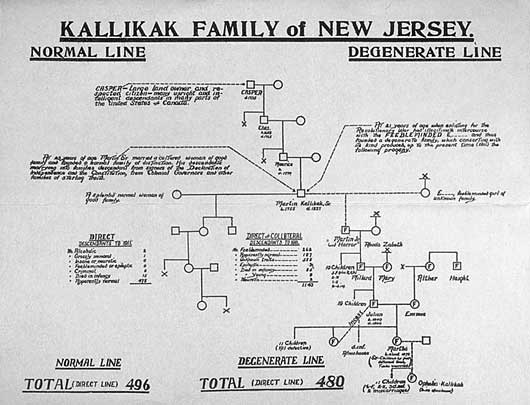
\includegraphics[width=0.75\linewidth]{images1/chart_Kallikak_pedigree2} 

}

\caption{Linhas "normais" e "degeneradas" da família Kallikak (New Jersey)}\label{fig:figA16}
\end{figure}

\hfill\break

\begin{figure}

{\centering 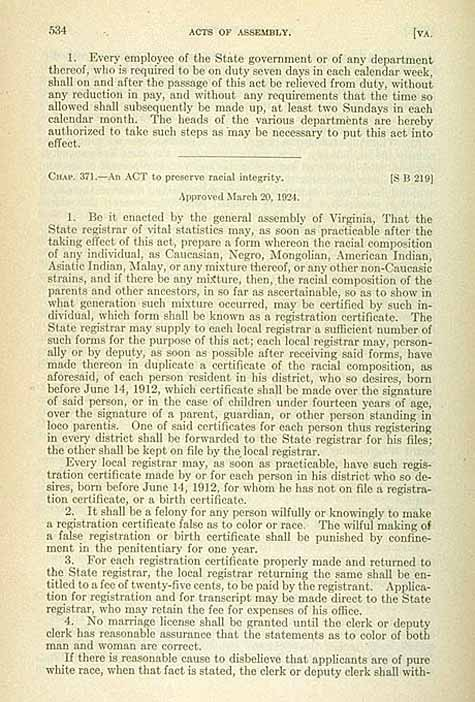
\includegraphics[width=0.75\linewidth]{images1/VA_racial_integrity_act2} 

}

\caption{Lei da Inegridade Racia (Virginia, EUA, 1924)}\label{fig:figA17}
\end{figure}

\hfill\break

\begin{figure}

{\centering 
\includegraphics[width=0.75\linewidth]{images1/choosing_love_over_eugenics} 

}

\caption{Licença para casamento}\label{fig:figA18}
\end{figure}

\hfill\break

\section{\texorpdfstring{Estatística e \emph{machine learning} : uma livre tradução deste \href{https://www.r-bloggers.com/2020/02/xgboostlss-an-extension-of-xgboost-to-probabilistic-forecasting/}{link}}{Estatística e machine learning : uma livre tradução deste link}}\label{estatuxedstica-e-machine-learning-uma-livre-traduuxe7uxe3o-deste-link}

\hfill\break

\begin{figure}

{\centering 
\includegraphics[width=0.8\linewidth]{images4/statData} 

}

\caption{Autor: estatístico anônimo}\label{fig:unnamed-chunk-5}
\end{figure}

\hfill\break

Para se raciocinar rigorosamente sob incerteza, precisamos invocar a linguagem da probabilidade (Zhang et al.~2020). Qualquer modelo que não forneça a quantificação da incerteza associada ao seu resultado provavelmente produzirá uma imagem incompleta e potencialmente enganosa.

\hfill\break

Embora este seja um consenso irrevogável na estatística, um equívoco comum, embora muito persistente, é que os algoritmos de \emph{machine learning} geralmente carecem de formas adequadas de quantificar a incerteza.

\hfill\break

Apesar do fato dos dois termos existirem em paralelo e serem indistintamente utilizados, a percepção de que algoritmos de \emph{machine learning} e a estatística implicam um conjunto de técnicas não sobrepostas permanece viva, tanto entre profissionais como acadêmicos.

\hfill\break

Isso é vividamente retratado pela declaração provocativa (e potencialmente irônica) de Brian D. Ripley de que ``o aprendizado de máquina é estatística menos qualquer verificação de modelos e suposições'' que ele fez durante a ``useR! 2004'', conferência de Viena que serviu para ilustrar a diferença entre aprendizado de máquina e estatística.

\hfill\break

Na verdade, a relação entre estatística e algoritmos de \emph{machine learning} é artificialmente complicada por tais afirmações e, na melhor das hipóteses, isto é lamentável, pois implica numa distinção profunda e qualitativa entre as duas disciplinas (Januschowski et al.~2020). O artigo de Leo Breiman (2001) é uma exceção notável, pois propõe diferenciar os dois com base na cultura científica, e não apenas nos métodos.

\hfill\break

Embora as abordagens discutidas em Breiman (2001) constituam uma divisão admissível do espaço de análise e modelação de dados, os avanços mais recentes tornaram gradualmente esta distinção menos clara.

\hfill\break

Na verdade, a tendência atual de investigação tanto em estatística com algoritmos de \emph{machine learning} gravita no sentido de aproximar ambas as disciplinas. Numa era de necessidade crescente de que os resultados dos modelos de previsão sejam transformados em conhecimentos explicáveis e confiáveis, este é um desenvolvimento extremamente promissor e encorajador, uma vez que ambas as disciplinas têm muito a aprender uma com a outra. Junto com Januschowski et al.~(2020) , argumentamos que é mais construtivo procurar um terreno comum do que introduzir fronteiras artificiais.

\chapter{Introdução conceitual essencial}\label{introduuxe7uxe3o-conceitual-essencial}

\hfill\break

\begin{quote}
``Estatística é a ciência de coletar, organizar, apresentar, analisar e interpretar dados{[}\ldots{]}'' (Ronald A. Fisher)
\end{quote}

\hfill\break

De modo geral, a estatística pode ser dividida em três grandes áreas:

\begin{itemize}
\tightlist
\item
  descritiva;
\item
  probabilidade; e,
\item
  inferencial.
\end{itemize}

\hfill\break

\section{Estatística descritiva}\label{estatuxedstica-descritiva}

Nos primeiros trabalhos estatísticos, os dados coletados eram inicialmente apresentados na forma de tabelas e gráficos.

A \textbf{estatística descritiva} se ocupa de tudo o que seja relacionado a dados: coleta, processamento, descrição (seja na forma tabular ou gráfica) e sínteses numéricas (de locação, de dispersão, de repartição) sem inferir coisa alguma além da informação trazida pelos dados. Vem experimentando crescente uso em todas as áreas científicas e desenvolvimento:

\begin{itemize}
\tightlist
\item
  crescente uso de uma abordagem quantitativa em todas as ciências;
\item
  disponibilidade de recursos computacionais;
\item
  quantidade de dados coletados.
\end{itemize}

A palavra \textbf{estatística} pode assumir diferentes significados:

\begin{itemize}
\tightlist
\item
  no singular: \textbf{estatística} \vspace{0.5cm}

  \begin{itemize}
  \tightlist
  \item
    refere-se à ciência que compreende métodos que são usados na coleta, análise, interpretação e apresentação de dados quantitativos ou qualitativos (numéricos ou não); e,
  \item
    denota uma medida ou fórmula específica (tais como uma média, um intervalo de valores, uma taxa de crescimento, um índice).
  \end{itemize}
\item
  no plural: \textbf{estatísticas}

  \begin{itemize}
  \tightlist
  \item
    refere-se a dados coletados de maneira sistemática com um propósito específico definido em qualquer campo de estudo (nesse sentido, as \emph{estatísticas} também podem ser consideradas como agregados de fatos expressos em forma numérica).
  \end{itemize}
\end{itemize}

\section{Estatística inferencial}\label{estatuxedstica-inferencial}

A \textbf{estatística inferencial} tem o objetivo de estabelecer níveis de confiança da tomada de decisão de associar uma estimativa amostral a um parâmetro populacional. Divide-se em estimação e testes de significância.

\begin{quote}
``Dedução e indução são procedimentos racionais que nos levam do já conhecido ao ainda não conhecido; isto é, permitem que adquiramos conhecimentos novos graças a conhecimentos já adquiridos.{[}\ldots{]}''
\end{quote}

Dedução.

Na dedução parte-se de uma verdade já conhecida para demonstrar que ela se aplica a todos os casos particulares iguais. Vai do geral ao particular.

Indução.

Na indução parte-se de alguns casos particulares iguais ou semelhantes para se estipular uma \textbf{lei geral}. Vai do particular ao geral.

Na dedução, dado \textbf{X}, infiro (concluo) \textbf{a}, \textbf{b}, \textbf{c}, \textbf{d}.

Na indução, dados \textbf{a}, \textbf{b}, \textbf{c}, \textbf{d}, infiro (concluo) \textbf{X}.

\begin{quote}
Exemplo: testes de aceleração (0-60 mph) feitos com 6 carros importados em 1999 resultaram nas seguintes medidas: 12,9 s; 16,50 s; 11,30 s; 15,20 s; 18,20 s e 17,70 s. Um estudo descritivo poderia afirmar que:
\end{quote}

\begin{itemize}
\tightlist
\item
  metade dos dados coletados acelera de 0-60 mph em menos de 16,00 s; e
\item
  a aceleração média de 0-60 mph é de 15,30 s.
\end{itemize}

\begin{quote}
Mas, a partir dessa amostra concluir que a aceleração média de \textbf{todos} os carros importados em 1999 seja de 15,30 s; ou, que \textbf{metade} dos carros importados em 1999 acelerem de 0-60 mph em menos de 16,00 s são afirmações que pertencem à \textbf{inferência estatística}.
\end{quote}

\section{Produção de conhecimento}\label{produuxe7uxe3o-de-conhecimento}

\begin{quote}
``A ciência não consegue provar coisa alguma. Ela pode apenas refutar as coisas {[}\ldots{]}'' (Karl Popper)
\end{quote}

\hfill\break

\begin{figure}

{\centering 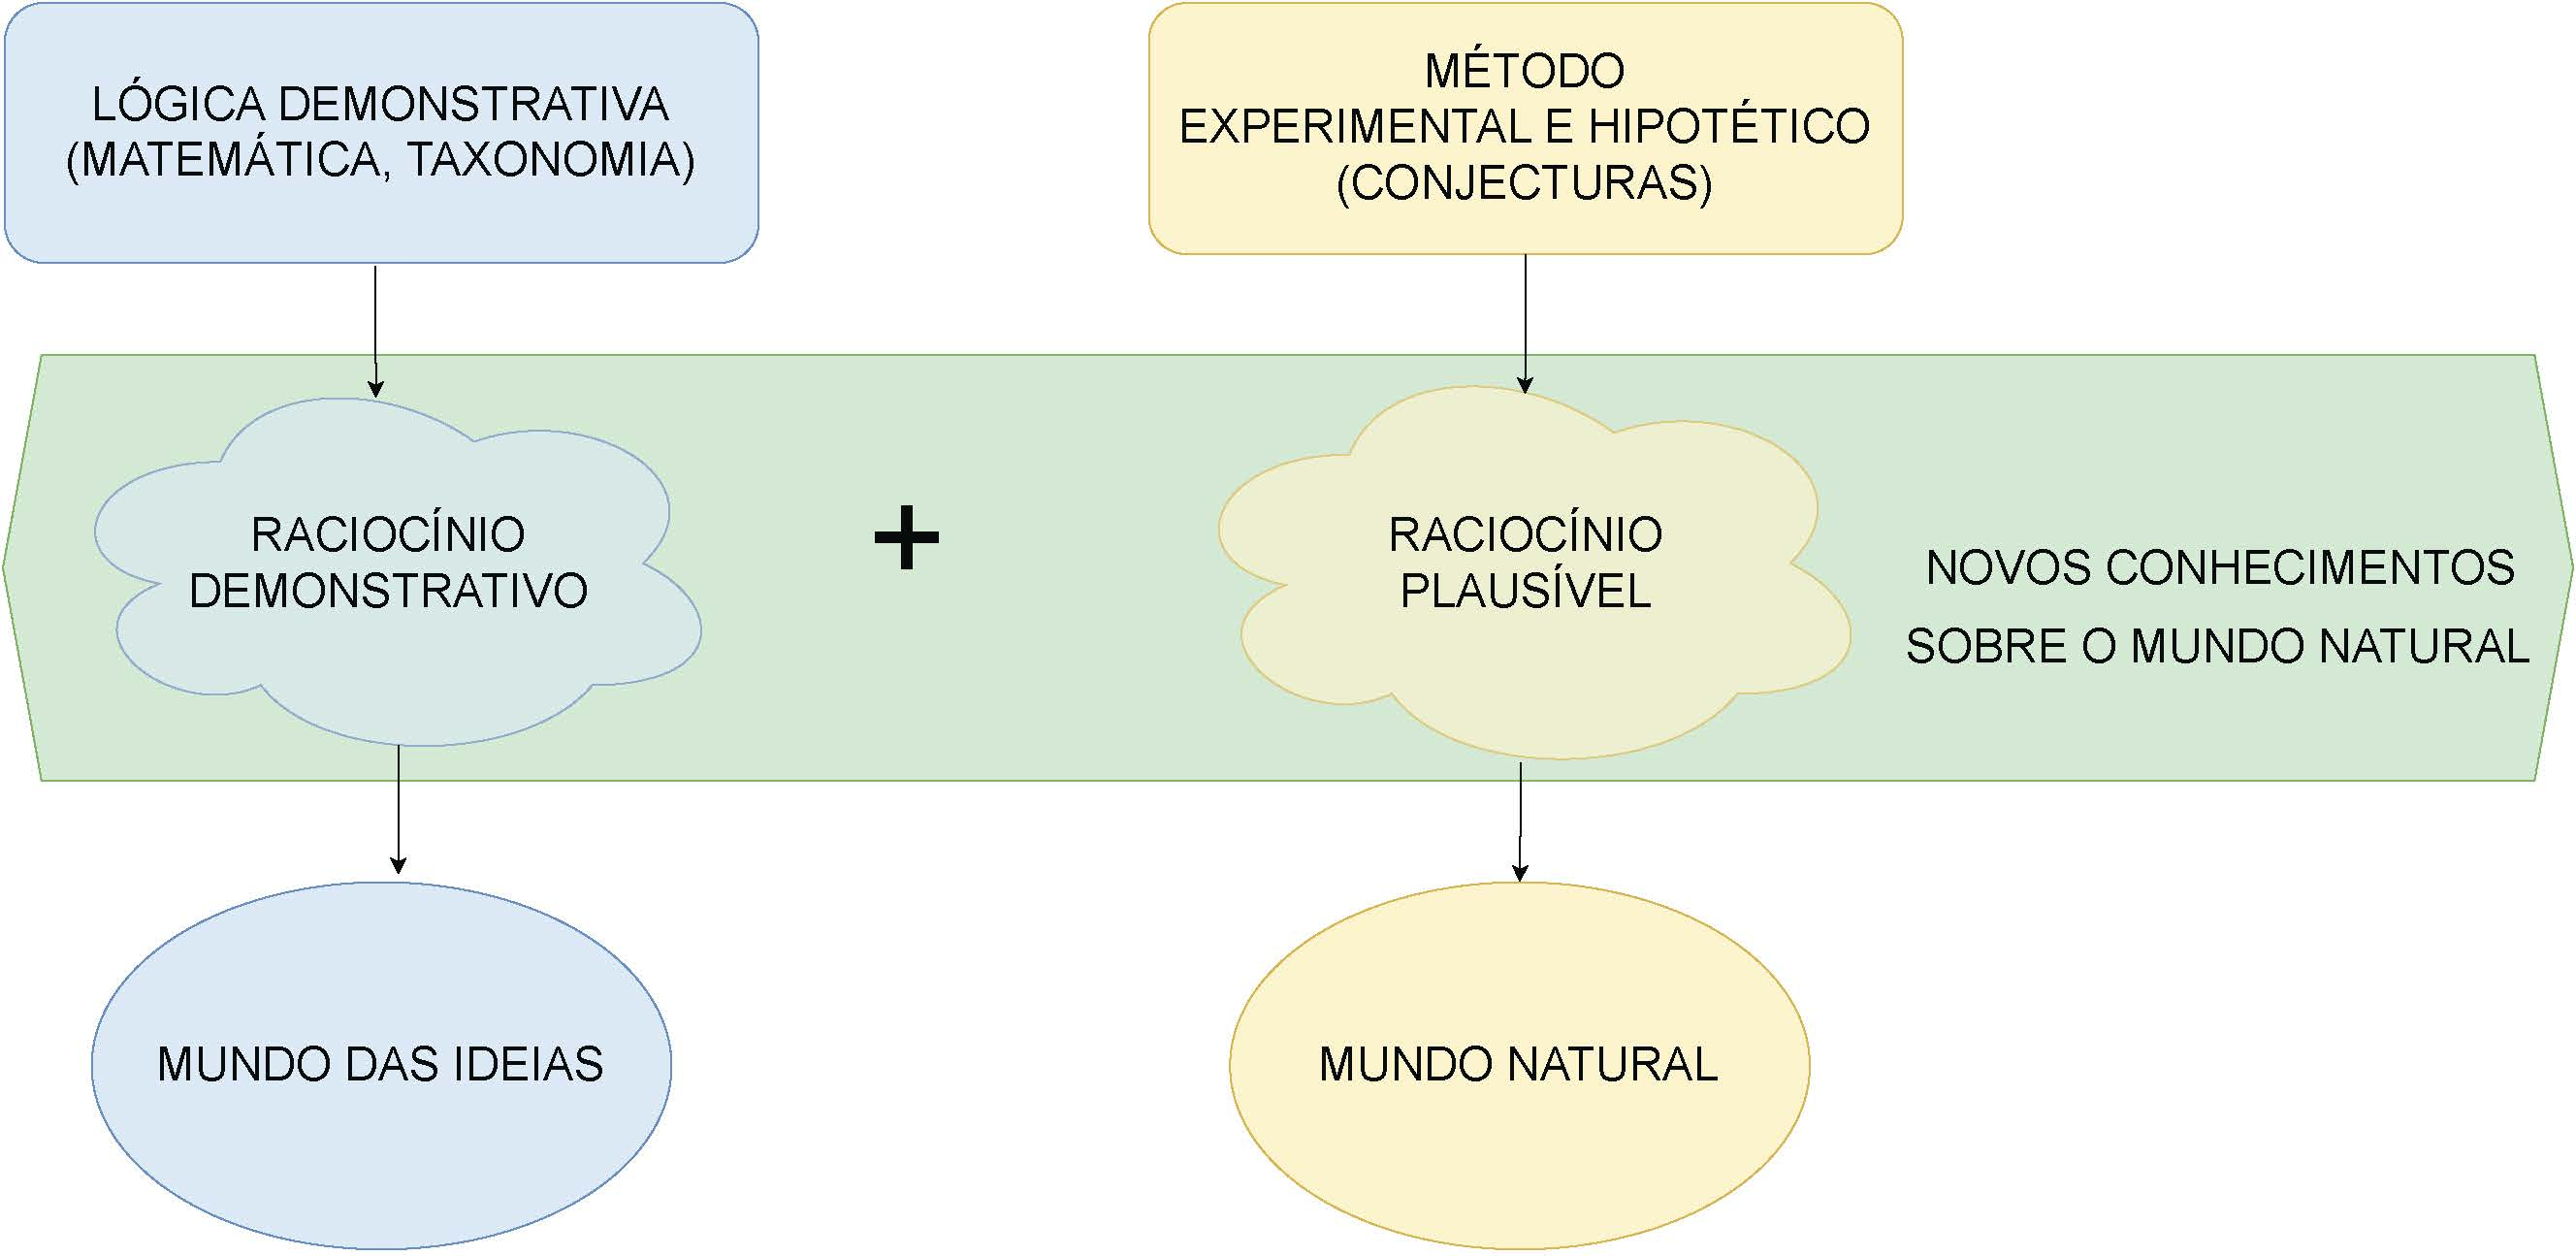
\includegraphics[width=1\linewidth]{images2/polya} 

}

\caption{Método demonstrativo e Método experimental hipotético (George Polya, 1954)}\label{fig:unnamed-chunk-7}
\end{figure}

\hfill\break

Na expansão de qualquer área do conhecimento propomos hipóteses que serão avaliadas mediante a coleta de dados que, depois de analisados, revelarão informações que, eventualmente, nos conduzirão ao afastamento da hipótese original e à proposição de outras, num processo contínuo.

\hfill\break

\begin{figure}

{\centering 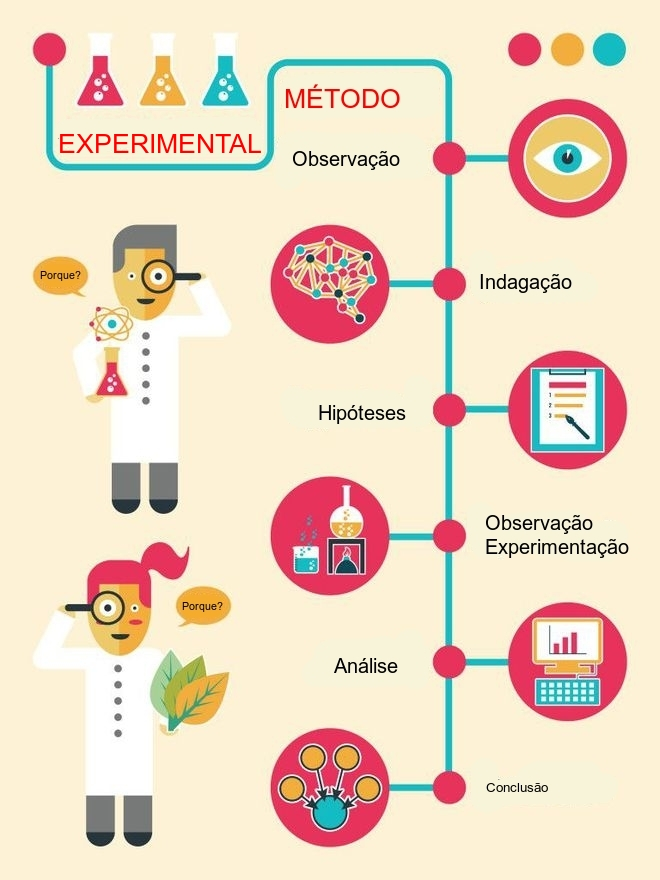
\includegraphics[width=0.6\linewidth]{images2/metodo_experimental} 

}

\caption{Método experimental hipotético}\label{fig:unnamed-chunk-8}
\end{figure}

\hfill\break

Uma investigação científica deve envolver, em linhas gerais:

\hfill\break

\begin{itemize}
\tightlist
\item
  observação dos fatos;
\item
  descrição das características essenciais, segundo o que se obteve através da observação;
\item
  explicação dessas características descritivas;
\item
  previsão; e,
\item
  decisão pertinente à investigação.
\end{itemize}

\hfill\break

O planejamento de uma pesquisa deve envolver, em linhas gerais:

\hfill\break

\begin{itemize}
\tightlist
\item
  definição do \emph{universo}: é necessário delimitar claramente, no tempo e espaço, o âmbito do inquérito, definindo, em termos precisos, o \emph{universo} a ser trabalhado;
\item
  exame das informações disponíveis: deve-se reunir todo o material existente: mapas, artigos, livros, relatórios relativos a levantamentos semelhantes;
\item
  tipos de levantamentos: completo ou amostral;
\item
  prazo;
\item
  custo;
\item
  precisão.
\end{itemize}

\section{População (universo) \& amostra}\label{populauxe7uxe3o-universo-amostra}

\hfill\break

\begin{figure}

{\centering 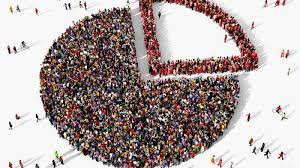
\includegraphics[width=1\linewidth]{images2/amostragem} 

}

\caption{Universo e amostra}\label{fig:unnamed-chunk-9}
\end{figure}

\hfill\break

Quase que, invariavelmente, em todo ramo de conhecimento, o pesquisador esbarra em uma série de limitações das mais variadas ordens (econômica, técnica, ética, geográfica, temporal,\ldots) que impossibilitam o estudo dos dados e informações associados a todos os casos existentes (\textbf{população ou universo}).

\hfill\break

Por essa razão, através de um procedimento estatístico denominado de amostragem, estuda-se uma população (universo) a partir de uma amostra. Amostra é, portanto, um subconjunto finito e representativo da população (universo), extraído de modo sistemático (planejado).

\section{Parâmetros e estatísticas}\label{paruxe2metros-e-estatuxedsticas}

\hfill\break

É comum a adoção de letras gregas para as características descritivas que se referirem à poúlação (universo) e letras do alfabeto latino para aquelas relativas à amostra extraída:

\hfill\break

\begin{longtable}[]{@{}lll@{}}
\toprule\noalign{}
Característica estudada & Notação populacional & Notação amostral \\
\midrule\noalign{}
\endhead
\bottomrule\noalign{}
\endlastfoot
Número de elementos & N & n \\
Média & \(\mu\) (``mi'') & \(\stackrel{-}{x}\) \\
Variância & \(\sigma^{2}\) (``sigma'') & \({s}^{2}\) \\
Desvio padrão & \(\sigma\) (``sigma'') & s \\
Proporção & \(\Pi\) (``pi'') & p ou \(\hat{p}\) \\
\end{longtable}

\hfill\break
\hfill\break
\hfill\break

\begin{figure}

{\centering 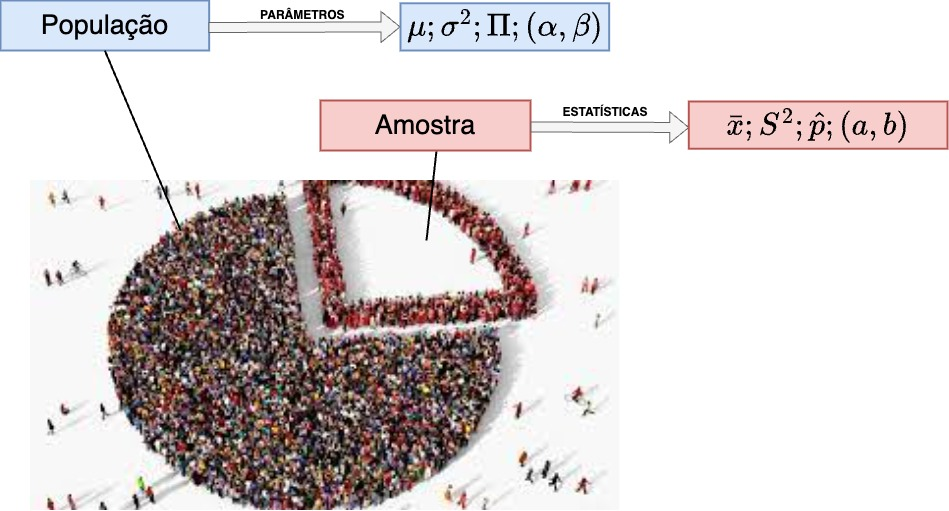
\includegraphics[width=1\linewidth]{images2/amostragem2} 

}

\caption{Parâmetros e estatísticas}\label{fig:unnamed-chunk-10}
\end{figure}

\hfill\break
\hfill\break
\hfill\break

\begin{figure}

{\centering 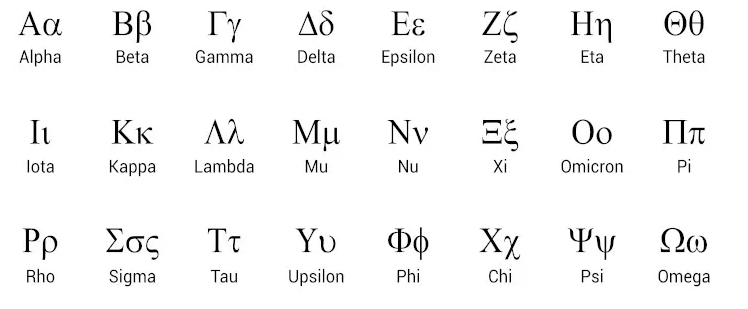
\includegraphics[width=1\linewidth]{images2/alf_grego} 

}

\caption{Alfabeto grego}\label{fig:unnamed-chunk-11}
\end{figure}

\section{Tipos de variáveis}\label{tipos-de-variuxe1veis}

\hfill\break

Variáveis quantitativas\\

\begin{itemize}
\tightlist
\item
  contínuas: são os dados com maior potencial de produzir informação significativa dentre todos: comprimentos, áreas, pesos, densidades; e,
\item
  discretas: são dados com um pouco menos de informação que os de natureza contínua mas possuem mais informação que dados qualitativos: número de andares de um prédio, de degraus de uma escada, número de filhos de um casal.
\end{itemize}

\hfill\break

Variáveis qualitativas

\hfill\break

\begin{itemize}
\tightlist
\item
  ordinais: apresentam um pouco mais de informação que os dados qualitativos puramente nominais na medida que suas classes podem ser interpretadas como possuindo um ordenamento inerente: padrão construtivo (baixo, médio, alto), classe econômica de rendimento (baixa, média, alta), nível de escolaridade (fundamental, médio e superior); e,
\item
  nominais: são dados a menor quantidade de informação: sexo, cor, códigos postais de cidades;
\end{itemize}

\hfill\break

Codificação de variáveis qualitativas

\hfill\break

\begin{itemize}
\tightlist
\item
  binárias: pela associação de valores numéricos: 0 ou 1 a uma variável qualitativa nominal que se apresente com apenas dois aspectos: sim ou não, ausência ou presença. Pela composição de mais variáveis binárias pode-se codificar variáveis que possuam um número maior de classes; e,
\item
  \emph{proxy}: pela associação de valores numéricos contínuos que guardam ``correlação'\,' com as classes da variável qualitativa nominal.
\end{itemize}

\begin{figure}

{\centering 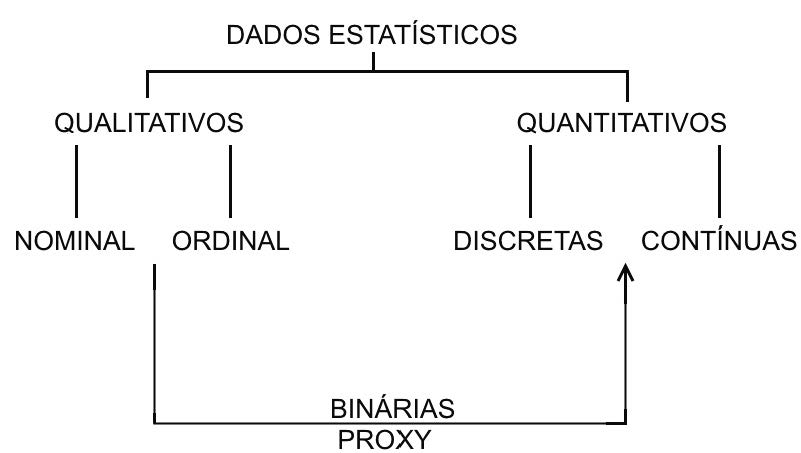
\includegraphics[width=0.75\linewidth]{images2/tipos_variaveis} 

}

\caption{Tipos e codificações de variáveis }\label{fig:unnamed-chunk-12}
\end{figure}

\section{\texorpdfstring{Indexação de dados (\(i\))}{Indexação de dados (i)}}\label{indexauxe7uxe3o-de-dados-i}

\hfill\break

Muitas operações matemáticas são representadas trazendo os valores dos dados indicados de modo genérico por letras (gregas ou romanas) e índices como, por exemplo, \(x_{i}\). Tal notação está a indicar que, se dispuséssemos os dados em uma linha virtual (às vezes necessitando que estejam ordenados, como para a determinação de uma separatiz), cada um de seus valores estaria a ocupar uma \emph{posição} indicada pelo índice \emph{i}:

\hfill\break

\begin{figure}

{\centering 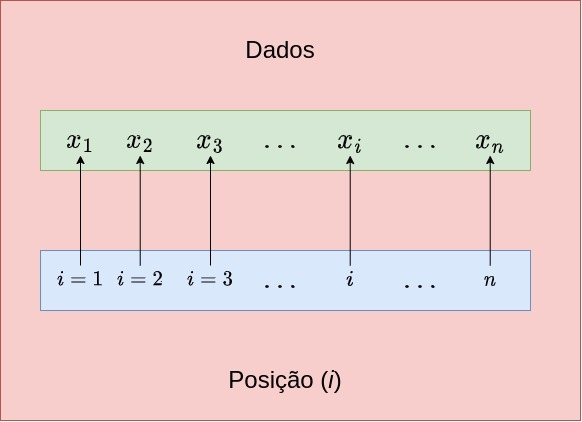
\includegraphics[width=0.6\linewidth]{images2/vetor_posicao} 

}

\caption{Entendendo a indexação de dados}\label{fig:unnamed-chunk-13}
\end{figure}

\section{\texorpdfstring{Noções básicas sobre somatórios (\(\Sigma\))}{Noções básicas sobre somatórios (\textbackslash Sigma)}}\label{nouxe7uxf5es-buxe1sicas-sobre-somatuxf3rios-sigma}

\hfill\break

Somatório é um operador matemático utilizado para simplificar expressões que envolvam soma de mais de um elemento.

\hfill\break

Digamos, por exemplo, que estamos interessados saber o total de comissões a pagar em um determinado setor de uma empresa.

\hfill\break

Admita que esse setor tenha 6 funcionários: Pedro, Guilherme, Lucas, Maria, Fernanda e Roberto e que suas comissões sejam R\$ 3000; R\$ 3300; R\$ 3900; R\$ 2950; R\$ 3150 e R\$ 3450.

\hfill\break

A representação da soma das comissões pode ser expressa de vários modos como, por exemplo, nesse extensa frase:

\hfill\break

\begin{quote}
O total de comissões a pagar em um determinado setor de uma empresa é a Renda do Pedro mais a Renda do Guilherme mais a Renda do Lucas mais a Renda da Maria mais a Renda da Fernanda mais Renda do Roberto.
\end{quote}

\hfill\break

Atribuindo os valores para cada uma das rendas:

\hfill\break

\begin{quote}
O total de comissões a pagar em um determinado setor de uma empresa é: : R\$ 3000 + R\$ 3300 + R\$ 3900 + R\$ 2950 + R\$ 3150 + R\$ 3450.
\end{quote}

\hfill\break

Chamando-se ``O total de comissões a pagar em um determinado setor de uma empresa é'' de \(X\), teremos:

\hfill\break

\begin{quote}
\(X\) = R\$ 3000 + R\$ 3300 + R\$ 3900 + R\$ 2950 + R\$ 3150 + R\$ 3450.
\end{quote}

\hfill\break

Para simplificar a representação dessa operação, vamos enumerar os funcionários: Pedro (1), Guilherme (2), Lucas (3), Maria (4), Fernanda (5) e Roberto (6). Além disso, vamos chamar a comissão a ser paga pela letra X.

\hfill\break

Para diferenciar a fração da comissão \(X\) a ser paga a cada um dos funcionários podemos por um índice na letra \(X\) para indicar a quem estamos nos referindo. Assim \(X_{1}\) seria a comissão do Pedro, \(X_{2}\) a do Guilherme, \(X_{3}\) a do Lucas, \(X_{4}\) a da Maria, \(X_{5}\) a da Fernanda e \(X_{3}\) a do Roberto.

\hfill\break

Com essa notação podemos representar matematicamente o total das comissões a pagar em um determinado setor de uma empresa por:

\hfill\break

\begin{quote}
\(X=X_{1}+X_{2}+X_{3}+X_{4}+X_{5}+X_{6}\)
\end{quote}

\hfill\break

Cada um desses fatores pode ser generalizado como um \(X_{i}\), a comissão de um \emph{i-ésimo} funcionário qualquer. Sabendo que o setor tem apenas 6 funcionários (Pedro, Guilherme, Lucas, Maria, Fernanda e Roberto) então esse i irá variar de 1 a 6 (Pedro:1, Guilherme: 2, Lucas: 3, Maria: 4, Fernanda: 5 e Roberto: 6).

\hfill\break

Com todas essas considerações podemos representar a soma das comissões utilizando a notação matemática do somatório.

\hfill\break

A letra grega maiúscula \textbf{\(\Sigma\) (``sigma'')} é habitualmente adotada na matemática para representar o somatório de uma quantidade de fatores. Assim, nosso exemplo da soma de 6 fatores (comissões) pode ser representada matematicamente por:

\hfill\break

\[
\sum_{i=1}^{6}{X_{i}} = X_{1}+X_{2}+X_{3}+X_{4}+X_{5}+X_{6}
\]

\hfill\break

Observe que abaixo da letra \(\Sigma\) (``sigma'') vemos \(i=1\) indicando que o índice dos fatores (X) a serem somados (a \emph{i-ésima} comissão) irá se iniciar pela comissão do primeiro funcionário, quando então i = 1.

\hfill\break

Acima da letra \(\Sigma\) (``sigma'') vemos o número \(6\) indicando que o índice dos fatores (X) a serem somados irá se dar até o valor da comissão do sexto funcionário, quando então i=6.

\hfill\break

Generalizando-se para uma soma de \(n\) fatores \(X\):

\hfill\break

\[
\sum_{i=1}^n{X_{i}}.
\]

\hfill\break

A representação matemática do somatório pode ser inserida junto a qualquer outra operação como, por exemplo, podemos, depois de realizar a soma, dividi-la por um valor \(n\) qualquer

\hfill\break

\[
\frac{\sum_{i=1}^n{X_{i}}}{n} \\
\]

\hfill\break

ou elevá-la ao quadrado:

\hfill\break

\[
\left(\sum_{i=1}^n{X_{i}}\right)^{2}
\]\\

Atenção para a diferença entre essas duas operações:

\hfill\break

\[
\left(\sum_{i=1}^n{X_{i}}\right)^{2}  
\]

\hfill\break

e

\hfill\break

\[
\sum_{i=1}^n{X_{i}^{2}}
\]\\

A primeira indica que devemos realizar a soma dos fatores \textbf{e só então elevar esse resultado ao quadrado}. A segunda indica que devemos realizar a \textbf{soma dos quadrados de cada um dos fatores}.

\hfill\break

\begin{Shaded}
\begin{Highlighting}[]
\FunctionTok{library}\NormalTok{(formattable)}
\NormalTok{comissoes}\OtherTok{=}\FunctionTok{c}\NormalTok{(}\DecValTok{3000}\NormalTok{, }\DecValTok{3300}\NormalTok{, }\DecValTok{3900}\NormalTok{, }\DecValTok{2950}\NormalTok{, }\DecValTok{3150}\NormalTok{, }\DecValTok{3450}\NormalTok{)}

\CommentTok{\#Somatório das comissões}
\FunctionTok{currency}\NormalTok{(}\FunctionTok{sum}\NormalTok{(comissoes),}
  \AttributeTok{symbol =} \StringTok{"R$"}\NormalTok{,}
  \AttributeTok{digits =} \DecValTok{2}\DataTypeTok{L}\NormalTok{,}
  \AttributeTok{format =} \StringTok{"f"}\NormalTok{,}
  \AttributeTok{big.mark=} \StringTok{"."}\NormalTok{,}
  \AttributeTok{decimal.mark=} \StringTok{","}\NormalTok{,}
  \AttributeTok{sep=} \StringTok{" "}\NormalTok{)}
\end{Highlighting}
\end{Shaded}

\begin{verbatim}
## [1] R$ 19.750,00
\end{verbatim}

\begin{Shaded}
\begin{Highlighting}[]
\CommentTok{\#Somatório das comissões dividido pelo número de comissões}
\FunctionTok{currency}\NormalTok{(}\FunctionTok{sum}\NormalTok{(comissoes)}\SpecialCharTok{/}\FunctionTok{length}\NormalTok{(comissoes),}
  \AttributeTok{symbol =} \StringTok{"R$"}\NormalTok{,}
  \AttributeTok{digits =} \DecValTok{2}\DataTypeTok{L}\NormalTok{,}
  \AttributeTok{format =} \StringTok{"f"}\NormalTok{,}
  \AttributeTok{big.mark=} \StringTok{"."}\NormalTok{,}
  \AttributeTok{decimal.mark=} \StringTok{","}\NormalTok{,}
  \AttributeTok{sep=} \StringTok{" "}\NormalTok{)}
\end{Highlighting}
\end{Shaded}

\begin{verbatim}
## [1] R$ 3.291,67
\end{verbatim}

\begin{Shaded}
\begin{Highlighting}[]
\CommentTok{\#Quadrado do somatório das comissões}
\FunctionTok{currency}\NormalTok{(}\FunctionTok{sum}\NormalTok{(comissoes)}\SpecialCharTok{\^{}}\DecValTok{2}\NormalTok{,}
  \AttributeTok{symbol =} \StringTok{"R$"}\NormalTok{,}
  \AttributeTok{digits =} \DecValTok{2}\DataTypeTok{L}\NormalTok{,}
  \AttributeTok{format =} \StringTok{"f"}\NormalTok{,}
  \AttributeTok{big.mark=} \StringTok{"."}\NormalTok{,}
  \AttributeTok{decimal.mark=} \StringTok{","}\NormalTok{,}
  \AttributeTok{sep=} \StringTok{" "}\NormalTok{)}
\end{Highlighting}
\end{Shaded}

\begin{verbatim}
## [1] R$ 390.062.500,00
\end{verbatim}

\begin{Shaded}
\begin{Highlighting}[]
\CommentTok{\#Somatório dos quadrados das comissões}
\FunctionTok{currency}\NormalTok{(}\FunctionTok{sum}\NormalTok{(comissoes}\SpecialCharTok{\^{}}\DecValTok{2}\NormalTok{),}
  \AttributeTok{symbol =} \StringTok{"R$"}\NormalTok{,}
  \AttributeTok{digits =} \DecValTok{2}\DataTypeTok{L}\NormalTok{,}
  \AttributeTok{format =} \StringTok{"f"}\NormalTok{,}
  \AttributeTok{big.mark=} \StringTok{"."}\NormalTok{,}
  \AttributeTok{decimal.mark=} \StringTok{","}\NormalTok{,}
  \AttributeTok{sep=} \StringTok{" "}\NormalTok{)}
\end{Highlighting}
\end{Shaded}

\begin{verbatim}
## [1] R$ 65.627.500,00
\end{verbatim}

\section{Análise combinatória (métodos de enumeração)}\label{anuxe1lise-combinatuxf3ria-muxe9todos-de-enumerauxe7uxe3o}

\hfill\break

A análise combinatória (ou métodos de enumeração) é um conjunto de técnicas para agrupamento de objetos conforme regras definidas e obtenção, através de cálculos, do número de agrupamentos possíveis.

\hfill\break

\subsection{Princípio básico da contagem (regra da multiplicação)}\label{princuxedpio-buxe1sico-da-contagem-regra-da-multiplicauxe7uxe3o}

\hfill\break

Suponha a realização de dois experimentos. Se o experimento \(E\) pode gerar qualquer um de \(n\) resultados possíveis (\(E_{1},E_{2},E_{3}, \dots, E_{n}\)) e se, para cada um dos resultados do experimento, houver \(m\) resultados possíveis para o experimento \(F\) (\(F_{1},F_{2},F_{3}, \dots, F_{m}\)), então os dois experimentos possuem conjuntamente \(n \cdot m\) diferentes resultados possíveis.

\hfill\break

\begin{figure}

{\centering 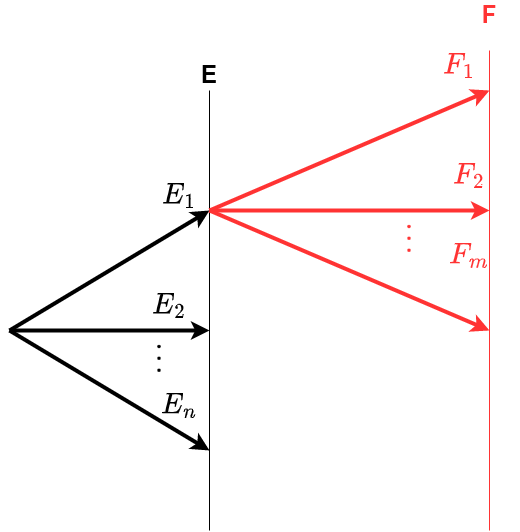
\includegraphics[width=0.5\linewidth]{images2/enumeracaoMultiplicacao} 

}

\caption{Regra da multiplicação}\label{fig:unnamed-chunk-15}
\end{figure}

\hfill\break

\begin{quote}
Esse princípio recebe o nome de \emph{Princípio multiplicativo}, e é aplicado nos casos em que os eventos são interligados pelo conectivo \textbf{e}, característico de decisões sucessivas: ocorrem os dois.
\end{quote}

\hfill\break

Se um homem tem 2 camisas e 4 gravatas, então ele tem \(2 \times  4 = 8\) formas de combinar uma camisa com uma gravata.

\hfill\break

Um diagrama como ilustrado na Figura \ref{fig:fig12} (denominado \textbf{diagrama de árvore} em virtude de sua aparência) geralmente é usado para explicar o princípio acima

\hfill\break

\begin{figure}

{\centering 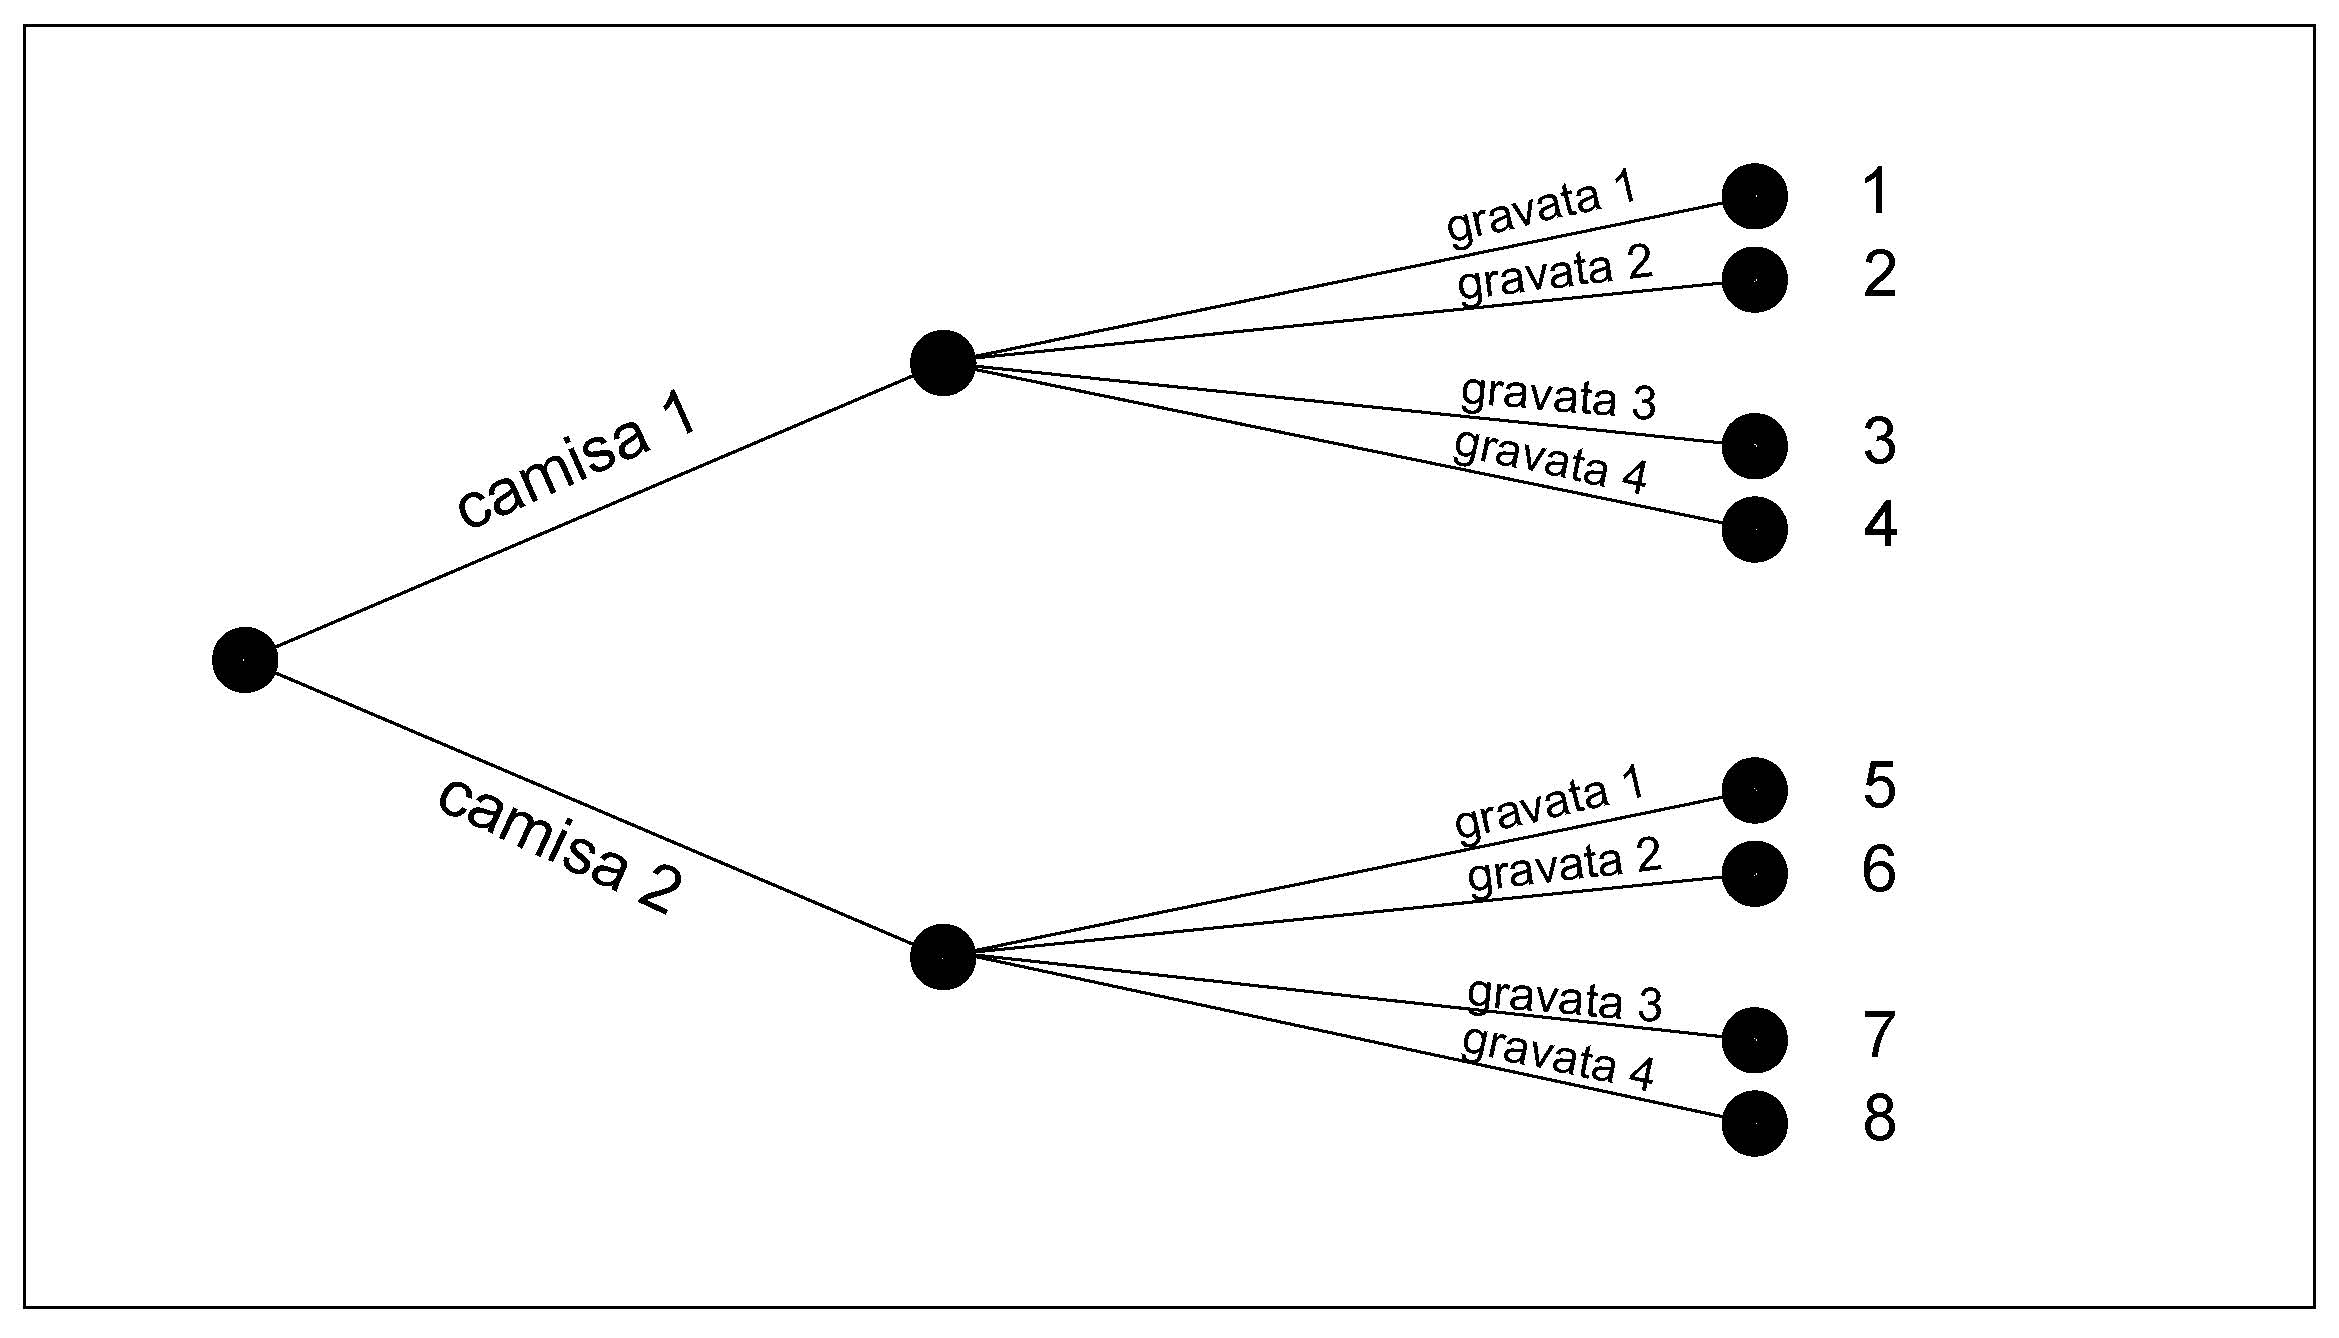
\includegraphics[width=0.5\linewidth]{images4/diagrama_arvore} 

}

\caption{Diagrama de árvore}\label{fig:fig12}
\end{figure}

\hfill\break

Ao lançarmos uma moeda três vezes (assumindo-se que K: cara e C: coroa) haverá \(2 \times  2 \times 2 = 8\) possibilidades distintas.

\hfill\break

O \textbf{diagrama de árvore} associado será (cf.~Figura \ref{fig:fig13}:

\hfill\break

\begin{figure}

{\centering 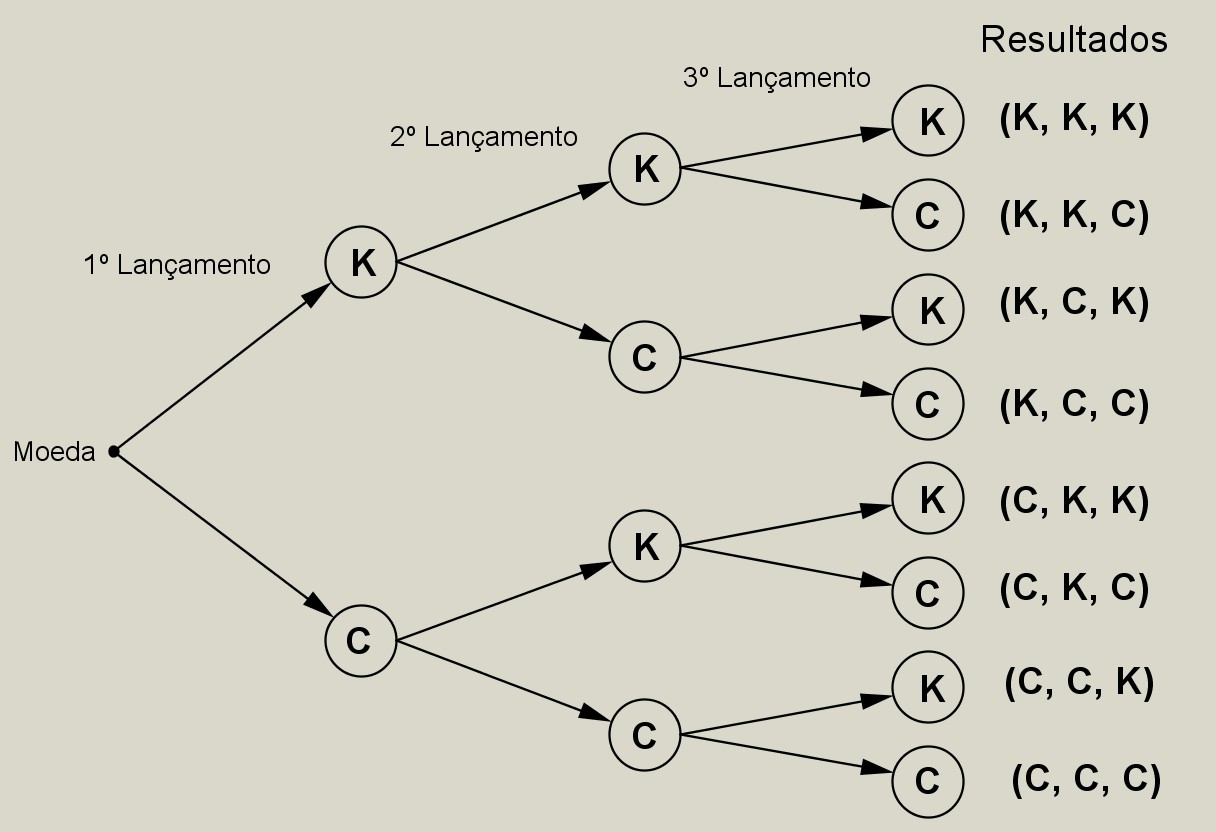
\includegraphics[width=0.5\linewidth]{images4/diagrama_arvore_moeda} 

}

\caption{Diagrama de árvore}\label{fig:fig13}
\end{figure}

\hfill\break

\subsection{Regra da adição}\label{regra-da-adiuxe7uxe3o}

\hfill\break

Suponha agora os mesmos expermentos \(E\) e \(F\) que geram \(n\) e \(m\) resultados possíveis (\(E_{1},E_{2},E_{3}, \dots, E_{n}\) e \(F_{1},F_{2},F_{3}, \dots, F_{m}\)), mas que eeses experimentos não estejam mais alinhados sequencialmente: ocorre o evento \(E\) ou o evento \(F\). Então o número de maneiras pelas quais o evento \(E\) ou o evento \(F\) poderão se manifestar será de \(n + m\) maneiras diferentes:

\hfill\break

\begin{figure}

{\centering 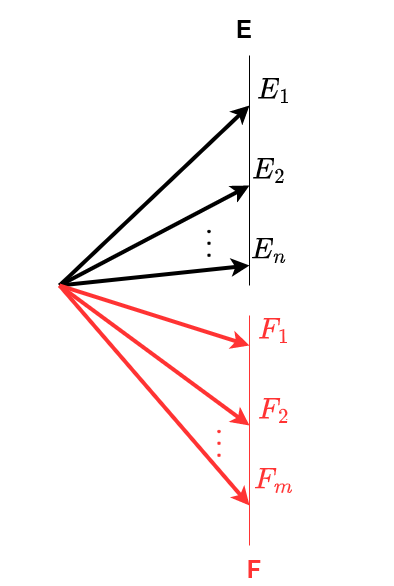
\includegraphics[width=0.5\linewidth]{images2/enumeracaoAdicao} 

}

\caption{Regra da adição}\label{fig:unnamed-chunk-16}
\end{figure}

\hfill\break

\begin{quote}
Esse princípio recebe o nome de \emph{Princípio aditivo}, e é aplicado nos casos em que os eventos são interligados pelo conectivo \textbf{ou}, característico de eventos mutuamente exclusivos: ocorre um ou outro.
\end{quote}

\hfill\break

Uma cantina de um colégio possui três tipos de sucos e dois tipos de refrigerantes. Um aluno pode adquirir apenas 1 suco ou 1 refrigerante. Quantas possibilidades de escolha ele tem?

\hfill\break

Seja \(E_{1}\) definido como escolher um tipo de suco (\(n_{1}=3\)) e \(E_{2}\) definido como escolher 1 tipo de refrigerante (\(n_{2}=2\)). Então o número total de possíveis escolhas será dado aplicando-se o princípio aditivo:

\hfill\break

\[
n_{1} + n_{2}=5
\]

\hfill\break

\subsection{Permutações (ordenação de elementos)}\label{permutauxe7uxf5es-ordenauxe7uxe3o-de-elementos}

\hfill\break

Suponha \(n\) objetos diferentes. Permutar os \(n\) objetos equivaleria a colocá-los dentro de uma caixa com \(n\) compartimentos em \textbf{alguma ordenação}.

\hfill\break

O primeiro compartimento pode ser ocupado por qualquer um dos \(n\) objetos, o segundo por \(n-1\) e o último por apenas 1 objeto.\\

Assim, pelo princípio básico vemos que essa caixa poderá ser carregada de:

\hfill\break

\[
n.(n-1).(n-2).1= n! \text{ maneiras diferentes.}
\].

\hfill\break

\begin{quote}
Exemplo: quantos diferentes arranjos ordenados das letras a, b e c são possíveis?
\end{quote}

\hfill\break

Pela enumeração direta vemos que são 6, ou seja, `abc', `acb', `bac', `bca', `cab' e `cba', resultado de \(3!=6\).

\hfill\break

\begin{quote}
Exemplo: quantas diferentes ordens de rebatedores são possíveis em um time de beisebol formado por 9 jogadores?
\end{quote}

\hfill\break

\(9! = 362.880\) ordenamentos possíveis para os rebatedores.

\hfill\break

\begin{quote}
Exemplo: uma turma de teoria da probabilidade é formada por 6 estudantes do sexo masculino e 4 do sexo feminino. Aplica-se uma prova e os estudantes são classificados de acordo com o seu desempenho. Suponha que nenhum dos estudantes tenha tirado a mesma nota.
(a) Quantas diferentes classificações são possíveis?
(b) Se os estudantes do sexo masculino forem classificados apenas entre si e também os do sexo feminino apenas entre si, quantas diferentes classificações são possíveis?
\end{quote}

\hfill\break

\begin{enumerate}
\def\labelenumi{\alph{enumi})}
\tightlist
\item
  Como cada classificação corresponde a um arranjo particular
  das 10 pessoas, a resposta é \(10! = 3.628.800\).
\end{enumerate}

\hfill\break

\begin{enumerate}
\def\labelenumi{(\alph{enumi})}
\setcounter{enumi}{1}
\tightlist
\item
  Como há \(6!\) possíveis classificações dos homens entre si e \(4!\) classificações possíveis das mulheres entre si, segue do princípio básico que há \((6!)(4!)=(720)(24) = 17.280\) classificações possíveis neste caso.
\end{enumerate}

\hfill\break

\subsection{Arranjos sem repetição}\label{arranjos-sem-repetiuxe7uxe3o}

\hfill\break

Considere um conjunto de \(n\) objetos diferentes. Suponha que desejamos selecionar uma quantidade \(p\) desses objetos, onde \(p < n\), e dispor os \(p\) objetos escolhidos em uma ordem específica.

\hfill\break

Quando selecionamos e ordenamos um subconjunto de objetos de um conjunto maior, estamos formando arranjos ordenados. Nesse caso, o número total de arranjos possíveis de \(p\) elementos retirados de um conjunto de \(n\) objetos distintos (\textbf{sem repetir nenhum elemento}) é dado por:

\[
P_{(n,p)} =  \frac{n!}{(n-p)!}
\]

\hfill\break

A fórmula para \(P_{(n,p)}\) considera tanto a seleção de \(p\) elementos quanto a ordenação deles, de modo que qualquer alteração na ordem dos elementos resulta em um novo arranjo.

\hfill\break

Dessa forma, arranjos com os mesmos objetos em ordens distintas são considerados distintos.

\hfill\break

\begin{quote}
Exemplo: quantos agrupamentos distintos, formados por 3 letras cada, podem ser formados com as 7 letras: A, B, C, D, E, F, G, considerando que não é permitido repetir nenhuma letra e que a ordem dos elementos importa?
\end{quote}

\hfill\break

\begin{align*}
n  & = 7 \\
p  & = 3 \\
P_{(n,p)} & = \frac{7!}{ (7-3)!} \\
          & = \frac{7!}{4!} = \\
          & = \frac{ 7 \times 6 \times 5 \times 4! }{4!}  \\
          & = 7 \times 6 \times 5  = 210   
\end{align*}

\hfill\break

\(ABC, ACB, BAC, BCA, CAB, CBA, \dots\)

\hfill\break

\subsection{Arranjos com repetição}\label{arranjos-com-repetiuxe7uxe3o}

\hfill\break

Considere um conjunto de \(n\) objetos diferentes. Suponha que desejamos selecionar uma quantidade \(p\) desses objetos, onde \(p < n\), e dispor os \(p\) objetos escolhidos em uma ordem específica.

\hfill\break

Ao permitirmos a repetição dos objetos no agrupamento, cada posição pode ser ocupada por qualquer um dos \(n\) objetos, independentemente das escolhas anteriores.

\hfill\break

Dessa forma, o número de arranjos com repetição de \(p\) elementos selecionados de um conjunto de nn objetos distintos é dado por:

\hfill\break

\[
P_{(n,p)} =  n ^{p}
\]\\

Essa fórmula ocorre porque, ao preencher cada uma das \(p\) posições com qualquer um dos \(n\) objetos, multiplicamos \(n\) possibilidades para cada posição, resultando em:

\hfill\break

\[
n \times n \times \ldots \times n = n^p
\]

\hfill\break

\begin{quote}
Exemplo: Quantos agrupamentos diferentes (onde a ordem dos elementos é razão para distinção: \textbf{permutações}) formados por \textbf{3 letras cada} podem ser formados com as \textbf{7 letras}: A, B, C, D, E, F, G \textbf{com repetição}?
\end{quote}

\hfill\break

\begin{align*}
n   &  = 7 \\
p   &  = 3 \\
P_{(n,p)} &  = n^{p} \\
          &   = 7 ^{3} = 343
\end{align*}

\hfill\break

Primeira posição: temos 7 opções (uma das 7 letras).
Segunda posição: também temos 7 opções, pois a repetição é permitida.
Terceira posição: novamente, temos 7 opções.

\hfill\break

\(AAA, AAB, AAC, \dots\)

\hfill\break

\subsection{Combinações sem repetição}\label{combinauxe7uxf5es-sem-repetiuxe7uxe3o}

\hfill\break

Em uma \emph{permutação}, a \emph{ordem} dos objetos em cada agrupamento é essencial: qualquer alteração na ordem cria um \textbf{agrupamento distinto}. Por exemplo, o agrupamento \emph{abc} é diferente de \emph{bca} numa permutação, pois a ordem importa.

\hfill\break

Em muitos problemas, entretanto, estamos interessados somente na seleção dos objetos, \textbf{sem considerar a ordem} em que eles aparecem.

\hfill\break

Nesse caso, os agrupamentos onde os mesmos elementos aparecem em \emph{ordens diferentes} são considerados \textbf{equivalentes}. Tais seleções são chamadas de combinações. Por exemplo, \emph{abc} e \emph{bca} representam uma mesma combinação, pois contêm os \textbf{mesmos} elementos \emph{independentemente da ordem}.

\hfill\break

O conceito de uma combinação refere-se a um conjunto de \(n\) objetos distintos, dos quais escolhemos \(p\) objetos \((p < n)\) \textbf{sem repetição}. Assim:

\begin{itemize}
\tightlist
\item
  \emph{a ordem} não importa: então \(abc\) é igual a \(bca\) (os agrupamentos que contêm os mesmos objetos em qualquer ordem \textbf{são considerados iguais});
\item
  \emph{a repetição} não permitida: cada objeto só aparece uma vez em cada agrupamento.
\end{itemize}

\hfill\break

O número total de combinações possíveis de \(p\) objetos selecionados de um conjunto de \(n\) objetos distintos é dado por:

\hfill\break

\[
C_{(n,p)} = \frac{n!}{p! \times (n-p)!}
\]\\

em que o \textbf{numerador} (\(n!\)) representa o número total de maneiras de permutar todos os \(n\) objetos, o \textbf{denominador} (\(p! \times (n - p)!\)) remove as redundâncias causadas pela permutação dos \(p\) objetos escolhidos (\(p!\)) e das maneiras de ordenar os \((n - p)\) objetos restantes (\((n - p)!\)).

\hfill\break

A fórmula resulta no número de agrupamentos únicos onde \textbf{apenas a composição do conjunto importa}, e a ordem dos elementos dentro de cada conjunto não afeta a contagem.

\hfill\break

\begin{quote}
Exemplo: Qual é número de formas nas quais \(3\) cartas podem ser escolhidas ou selecionadas de um total de \(8\) cartas diferentes?
\end{quote}

\hfill\break

\begin{align*}
n & = 8 \\
p & = 3 \\
C_{(n,p)} & = \frac{n!}{p! \times (n - p)!}\\
C_{(8,3)} & = \frac{8!}{ 3! (8-3)!}  \\
          & = \frac{8!}{3! \times 5!} \\
          & = \frac{ 8 \times 7 \times 6 \times 5! }{ 3! \times 5! } \\
          & = \frac{ 8 \times 7 \times 6 }{3!} = 56  
\end{align*}

\hfill\break

O número total de combinações com repetição, de \(p\) objetos selecionados de \(n\) (também chamado de combinações de \(n\) elementos tomados \(p\) a cada vez com repetição) é representado por:

\hfill\break

\[
C_{(n+p-1,p)} = \frac{ (n+p-1)! }{ p! \times ( n-1)!}
\]

\hfill\break

\begin{quote}
Exemplo: um comitê de três pessoas deve ser formado a partir de um grupo de 20 pessoas. Quantos comitês diferentes são possíveis?
\end{quote}

\hfill\break

\begin{align*}
n & =  20 \\
p & = 3 \\ 
C_{(n,p)} & = \frac{n!}{p! \times (n - p)!}\\
C_{(20,3)} & = \frac{20!}{3! \times (20 - 3)!}\\
& = \frac{20 \times 19 \times 18 \times 17!}{3! \times 17!}\\
& = \frac{20 \times 19 \times 18}{3 \times 2 \times 1}\\
& = \frac{6840}{6} = 1140
\end{align*}

\hfill\break

\begin{quote}
Exemplo: de um grupo de cinco mulheres e sete homens, quantos comitês diferentes formados por duas mulheres e três homens podem ser formados? E se dois dos homens estiverem brigados e se recusarem a trabalhar juntos?
\end{quote}

\hfill\break

Para resolver esse problema, vamos dividi-lo em duas partes:

\begin{enumerate}
\def\labelenumi{\arabic{enumi}.}
\tightlist
\item
  calcular o número de comitês possíveis formados por duas mulheres e três homens (combinações \(C_{(5,2})\) e \(C_{(7,3})\))
\item
  Calcular o número de comitês possíveis se dois dos homens estiverem brigados e se recusarem a trabalhar juntos.
\end{enumerate}

\hfill\break

\begin{quote}
Parte 1: Comitês sem restrição
\end{quote}

\textbf{Escolha das Mulheres}: Temos 5 mulheres e precisamos escolher 2. O número de maneiras de fazer isso é uma combinação, dada por:

\hfill\break

\[
C_{(5, 2)} = \frac{5!}{2! \times (5 - 2)!} = \frac{5 \times 4}{2 \times 1} = 10
\]\\

\textbf{Escolha dos Homens}: Temos 7 homens e precisamos escolher 3. O número de maneiras de fazer isso também é uma combinação, dada por:

\[
C_{(7, 3)} = \frac{7!}{3! \times (7 - 3)!} = \frac{7 \times 6 \times 5}{3 \times 2 \times 1} = 35
\]\\

O \textbf{número total de comitês} é o produto das duas combinações (princípio básico):

\[
\text{Total} = C_{(5, 2)} \times C_{(7, 3)} = 10 \times 35 = 350
\]\\

Portanto, sem restrições, há \textbf{350 comitês diferentes} que podem ser formados.

\hfill\break

\begin{quote}
Parte 2: Comitês com restrição (Dois Homens Brigados)
\end{quote}

\hfill\break

Para calcular o número de comitês possíveis com essa restrição, usamos o princípio da exclusão: (total de comitês sem restrição - total de comitês com restrição). Começamos contando quantos comitês incluem os dois homens brigados: \(A\) e \(B\).

\hfill\break

Se ambos estão no comitê então precisamos escolher apenas mais 1 homem entre os 5 homens restantes. O número de maneiras de fazer isso é:

\hfill\break

\[
C_{(5, 1)} = 5
\]\\

Então, do total de \textbf{35 possíveis grupos de 3 homens formados sem restrição} apenas 5 são grupos onde \(A\) e \(B\) estão presentes, resultando então em \(35-5=30\) grupos onde \(A\) e \(B\) estão ausentes.

\hfill\break

Compondo com o número de possíveis grupos de mulheres (princípio básico) teremos:

\hfill\break

\[
\text{Total} = C_{(5, 2)} \times30 = 10 \times 30 = 300
\]\\

Portanto, com essa restriçãose, há \textbf{300 comitês diferentes} que podem ser formados.

\hfill\break

\subsection{Combinações com Repetição}\label{combinauxe7uxf5es-com-repetiuxe7uxe3o}

\hfill\break

Em muitos problemas de contagem, estamos interessados em \textbf{selecionar} um subconjunto de objetos de um conjunto maior, sem nos preocupar com a ordem dos objetos. Isso é chamado de \textbf{combinação}. No entanto, ao contrário das combinações convencionais, em alguns casos é permitido que os mesmos objetos sejam escolhidos mais de uma vez. Essas são conhecidas como \textbf{combinações com repetição}.

\hfill\break

Nas \textbf{combinações com repetição}, selecionamos \(p\) objetos a partir de um conjunto de \(n\) objetos distintos, \textbf{permitindo} que cada objeto seja escolhido mais de uma vez. Nesse contexto: a \textbf{ordem dos objetos não importa}, ou seja, uma seleção de \emph{A,B,A} é considerada igual a \emph{A,A,B} e a \textbf{repetição é permitida}, então podemos escolher o mesmo objeto mais de uma vez.

\hfill\break

Combinações com repetição são úteis em contextos onde é necessário selecionar subconjuntos com elementos repetidos, como:
- escolha de itens com reposição (como selecionar moedas em valores específicos).
- problemas de contagem em álgebra combinatória.
- distribuição de recursos em cenários onde itens podem ser alocados mais de uma vez.

\hfill\break

O número de combinações \textbf{com repetição} para selecionar \(p\) objetos de um conjunto de \(n\) objetos distintos é dado por:

\hfill\break

\[
C_{(n + p - 1, p)} = \frac{(n + p - 1)!}{p! \times (n - 1)!}
\]

\hfill\break

Essa fórmula reflete o fato de que, ao permitir repetições, cada seleção possível pode ser visualizada como uma combinação com um conjunto ``expandido'' de opções, onde as escolhas de um mesmo objeto múltiplas vezes são válidas e contadas.

\hfill\break

\begin{quote}
Exemplo: quantas maneiras existem de selecionar 3 frutas de um conjunto com 5 tipos diferentes (maçã, banana, laranja, uva e pera), onde repetições são permitidas?
\end{quote}

\hfill\break

\begin{align*}
n & = 5 \\
p & = 3 \\
C_{(n + p - 1, p)} & = \frac{(n + p - 1)!}{p! \times (n - 1)!}\\
C_{(5 + 3 - 1, 3)} & = \frac{(5 + 3 - 1)!}{3! \times (5 - 1)!} = \frac{7!}{3! \times 4!}\\
& = \frac{7 \times 6 \times 5 \times 4!}{3! \times 4!} = \frac{7 \times 6 \times 5}{3 \times 2 \times 1} = \frac{210}{6} = 35
\end{align*}

\hfill\break

\begin{quote}
Exemplo: supondo que você queira comprar um sorvete com 4 bolas em uma sorveteria que possui 3 sabores disponíveis: chocolate, baunilha e morango. De quantos modos diferentes você pode fazer esta compra? (Note que nesta combinação é possível repetir a ordem de dois ou mais sabores, assim tratando de uma combinação com repetição).
\end{quote}

\hfill\break

\begin{align*}
n & =  3 \\
p & = 4 \\ 
C_{(n + p - 1, p)} & = \frac{(n + p - 1)!}{p! \times (n - 1)!}\\
C_{(n+p-1,p)} & = \frac{(3+4-1)!}{ 4! (3-1)!} = 15  
\end{align*}

\hfill\break

\section{Fatoriais}\label{fatoriais}

\begin{quote}
\(n!=n.(n-1).(n-2)\dots(n-(n-1)).(n-n)\)
\end{quote}

\begin{quote}
\(1!=1\)
\end{quote}

\begin{quote}
\(0!=1\)
\end{quote}

\begin{align*}
P_{(n,n)} & = \frac{n!}{(n-n)!} = \frac{n!}{0!} = n! \\
C_{(n,0)} & = \frac{n!}{ 0! \times (n-0)! } = \frac{n!}{ 1 \times (n)!} = 1 \\
C_{(n,1)} & = \frac{n! }{ 1! (n-1)!} \\
   & = \frac{ n! }{(n-1)! } \\
   & = \frac{ n \times (n-1)! }{ (n-1)!} = n    
\end{align*}

\section{Conectivos lógicos}\label{conectivos-luxf3gicos}

Muitos dos problemas ligados à probabilidade de ocorrência de eventos são propostos com o auxílio de conectivos lógicos:

\hfill\break

\begin{itemize}
\tightlist
\item
  \textbf{Proposição}: a afirmação de que algo é verdadeiro. Após analisarmos qualquer proposição, podemos defini-la como verdadeira ou falsa como, por exemplo: ``o céu é azul'';
\item
  \textbf{Negação}: negação do valor lógico de uma proposição. A negação de uma proposição verdadeira é falsa. A negação de uma proposição falsa é verdadeira. Os símbolos da negação são o til \(^{-}\) ou \(^{c}\);
\item
  \textbf{Conjunção}: proposição composta com a utilização do conectivo ``e'' como, por exemplo: ``o céu é azul e as nuvens são brancas''. Os símbolos usuais para uma conjunção são: \(\cap\) ou a letra ``V'' invertida; e,
\item
  \textbf{Disjunção}: proposição composta com a utilização do conectivo ``ou'' como, por exemplo, ``o céu é azul ou os pássaros são pretos''. Os símbolos usuais para uma disjunção são: \(\cup\) ou a letra \(V\).
\end{itemize}

\section{Leis de De Morgan}\label{leis-de-de-morgan}

Augustus de Morgan foi um matemático e lógico indiano.

\hfill\break

\begin{figure}

{\centering 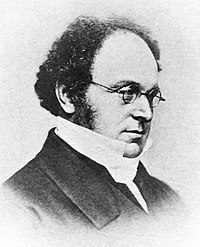
\includegraphics[width=0.5\linewidth]{images4/de_morgan} 

}

\caption{Augustus De Morgan (1806 - 1871)}\label{fig:unnamed-chunk-17}
\end{figure}

\hfill\break

Primeira Lei de De Morgan:

\hfill\break

Negar duas proposições ligadas com ``e'' (\(\cap\)); ou seja, uma \textbf{conjunção}, é o mesmo que negar duas proposições e ligá-las com ``ou''\,' (ou seja, transformá-las em uma disjunção). Considerando as proposições ``p'' e ``q'' teremos:

\hfill\break

\begin{itemize}
\tightlist
\item
  \(\sim (p \cap q) = (~p) \cup (~q)\); ou,\\
\item
  \((p \cap q)^{c} = (p^{c}) \cup (q^{c})\).
\end{itemize}

\hfill\break

Segunda Lei de De Morgan:

\hfill\break

Negar duas proposições ligadas por ``ou''\,' (\(\cup\)); ou seja, uma \textbf{disjunção}, é o mesmo que negar as duas proposições e ligá-las com ``e'' (ou seja, transformá-las em uma conjunção). Considerando as proposições ``p'' e ``q'' teremos:

\hfill\break

\begin{itemize}
\tightlist
\item
  \(\sim (p \cup q) = (~p) \cap (~q)\); ou,\\
\item
  \((p \cup q)^{c}= (p^{c}) \cap (q^{c})\).
\end{itemize}

\section{Noções básicas para o uso de calculadora (Cassio fx-82MS)}\label{nouxe7uxf5es-buxe1sicas-para-o-uso-de-calculadora-cassio-fx-82ms}

Em estatística trabalha-se muito com a análise de um ou mais conjuntos de dados, sendo comum a realização de diversas operações matemáticas com esses dados. Muitas dessas operações envolvem somatórios, por exemplo, e para simplificar essas operações o uso da calculadora se torna essencial.

Neste curso recomenda-se o uso de uma calculadora científica. Existem diversas calculadoras que cumprem as funções necessárias nesse curso. Para padronizar as aulas, alguns professores sugerem a calculadora científica de código: FX82MS, que é a calculadora que cujo funcionamento será exibido a seguir, passo a passo. A seguir serão descritas algumas das funções básicas mais importantes no uso desta calculadora.

Primeiro vamos deixar a calculadora no modo de regressão linear. Esse modo permite que a calculadora
funcione normalmente para as operações comuns (soma, subtração, multiplicação e divisão), e ainda libera
todas as funções importantes nesse curso. Sempre que o aluno for utilizar a calculadora, ele deve se certificar que ela esteja no modo de regressão linear, da seguinte forma:

PASSO 1:

\begin{itemize}
\tightlist
\item
  \begin{enumerate}
  \def\labelenumi{\arabic{enumi}.}
  \tightlist
  \item
    ON
  \end{enumerate}
\item
  \begin{enumerate}
  \def\labelenumi{\arabic{enumi}.}
  \setcounter{enumi}{1}
  \tightlist
  \item
    MODE
  \end{enumerate}
\item
  \begin{enumerate}
  \def\labelenumi{\arabic{enumi}.}
  \setcounter{enumi}{2}
  \tightlist
  \item
    Aperte 3 para escolher REG
  \end{enumerate}
\item
  \begin{enumerate}
  \def\labelenumi{\arabic{enumi}.}
  \setcounter{enumi}{3}
  \tightlist
  \item
    Aperte 1 para escolher LIN
  \end{enumerate}
\end{itemize}

Repare que no topo do visor da calculadora apareceu o símbolo \textcolor{red}{REG}, que indica que a calculadora está em modo de regressão. Desde que esteja no modo de regressão, podemos passar para o passo seguinte.

O nosso objetivo aqui é inserir o conjunto de dados na calculadora para então realizarmos as operações necessárias. Mas antes de inserir os dados, temos que garantir que a calculadora esteja \textcolor{red}{vazia} para o novo conjunto de dados. Ou seja, devemos limpar a calculadora:

PASSO 2:

\begin{itemize}
\tightlist
\item
  \begin{enumerate}
  \def\labelenumi{\arabic{enumi}.}
  \tightlist
  \item
    SHIFT
  \end{enumerate}
\item
  \begin{enumerate}
  \def\labelenumi{\arabic{enumi}.}
  \setcounter{enumi}{1}
  \tightlist
  \item
    MODE
  \end{enumerate}
\item
  \begin{enumerate}
  \def\labelenumi{\arabic{enumi}.}
  \setcounter{enumi}{2}
  \tightlist
  \item
    Aperte 1 para escolher Scl ( \emph{Stat Clear})
  \end{enumerate}
\item
  \begin{enumerate}
  \def\labelenumi{\arabic{enumi}.}
  \setcounter{enumi}{3}
  \tightlist
  \item
    Aperte = para limpar a calculadora
  \end{enumerate}
\end{itemize}

Entrada de dados.

Agora que a calculadora está em modo de regressão e está limpa, podemos inserir o conjunto de dados. Para ilustrar esta função, vamos inserir o seguinte conjunto de dados: \(X= {5,3,6,2}\).

Para inserir cada um desses elementos você deve digitar o número e em seguida o botão M+.

A sequência fica assim: 5 M+ 3 M+ 6 M+ 2 M+.

A cada vez que você insere uma observação, a calculadora atualiza o número de observações inseridas. No final, nesse caso, aparece \textcolor{red}{n=4} porque inserimos 4 observações.

Funções envolvendo somatórios.

Observe na calculadora os botões \textcolor{orange}{shift} e \textcolor{red}{alpha}. Geralmente estes botões aparecem nas cores amarela e vermelha, respectivamente. Observe ainda que alguns botões da calculadora possuem termos nessas cores. Para selecionar as funções em \textcolor{orange}{amarelo}, antes devemos ligar o modo \textcolor{orange}{shift}. Enquanto que para selecionar as funções em \textcolor{red}{vermelho} deve-se ligar o modo \textcolor{red}{alpha}.

Por exemplo, para abrir a função \textcolor{orange}{S-SUM} que está em \textcolor{orange}{amarelo} no botão 1, faz-se: SHIFT 1. A função \textcolor{orange}{S-SUM} é a que contém todos os somatórios importantes. Ao abrir esta função aparecem três opções da seguinte forma:

\[
\Sigma(x) \\
\Sigma(x^{2})\\
n 
\]

Aperta-se 1 = para ter o somatório de \(x\); 2 = para ter o somatório de \(x^{2}\) ou 3 = para saber o número \(n\) de obervações inseridas.

Funções para obter a média e o desvio padrão.

A função \textcolor{orange}{S-VAR} fornece a média e o desvio padrão dos dados. Essas são medidas importantes, que serão utilizadas durante todo o curso. Para abrir esta função faz-se: SHIFT 2.

\[
\stackrel{-}{x}
\sigma_{x}
S_{x}
\]

A opção 1 retorna a média dos dados, a opção 2 retorna o desvio padrão populacional e a opção 3 o desvio padrão amostral.

Como inserir dois conjuntos de dados.

Quando se deseja estudar dois conjuntos de dados, de mesmo tamanho, pode-se inseri-los de forma simultânea na calculadora. Para ilustrar vamos inserir os seguintes conjuntos de dados: \(X={2,7,4,3,2}\) e \(Y={1,2,3,6,5}\). \textcolor{red}{Antes de inserir os dados, lembre-se de limpar a calculadora}.

Em seguida vamos inserir os dados de 2 em 2: o primeiro de X com o primeiro de Y e assim por diante. Repare que ao lado do botão M+ tem um botão com uma vírgula. Esta vírgula é utilizada para separar as observações de X das de Y . A sequência fica assim:

\begin{itemize}
\tightlist
\item
  2,1 M+
\item
  7,2 M+
\item
  4,3 M+
\item
  3,6 M+
\item
  2,5 M+
\end{itemize}

Se você usar a função \textcolor{orange}{S-SUM}, na tela vai aparecer os somatórios apenas de X, que foi pela ordem, o primeiro a ser inserido. Na calculadora tem um botão grande e style=``color:gray;''\textgreater S-SUM, com 4 setas. Depois de selecionar a função \textcolor{orange}{amarelo} aperte a seta para frente que aparecerão os somatórios para Y . O mesmo acontece para a função \textcolor{orange}{S-VAR}.

\begin{figure}

{\centering 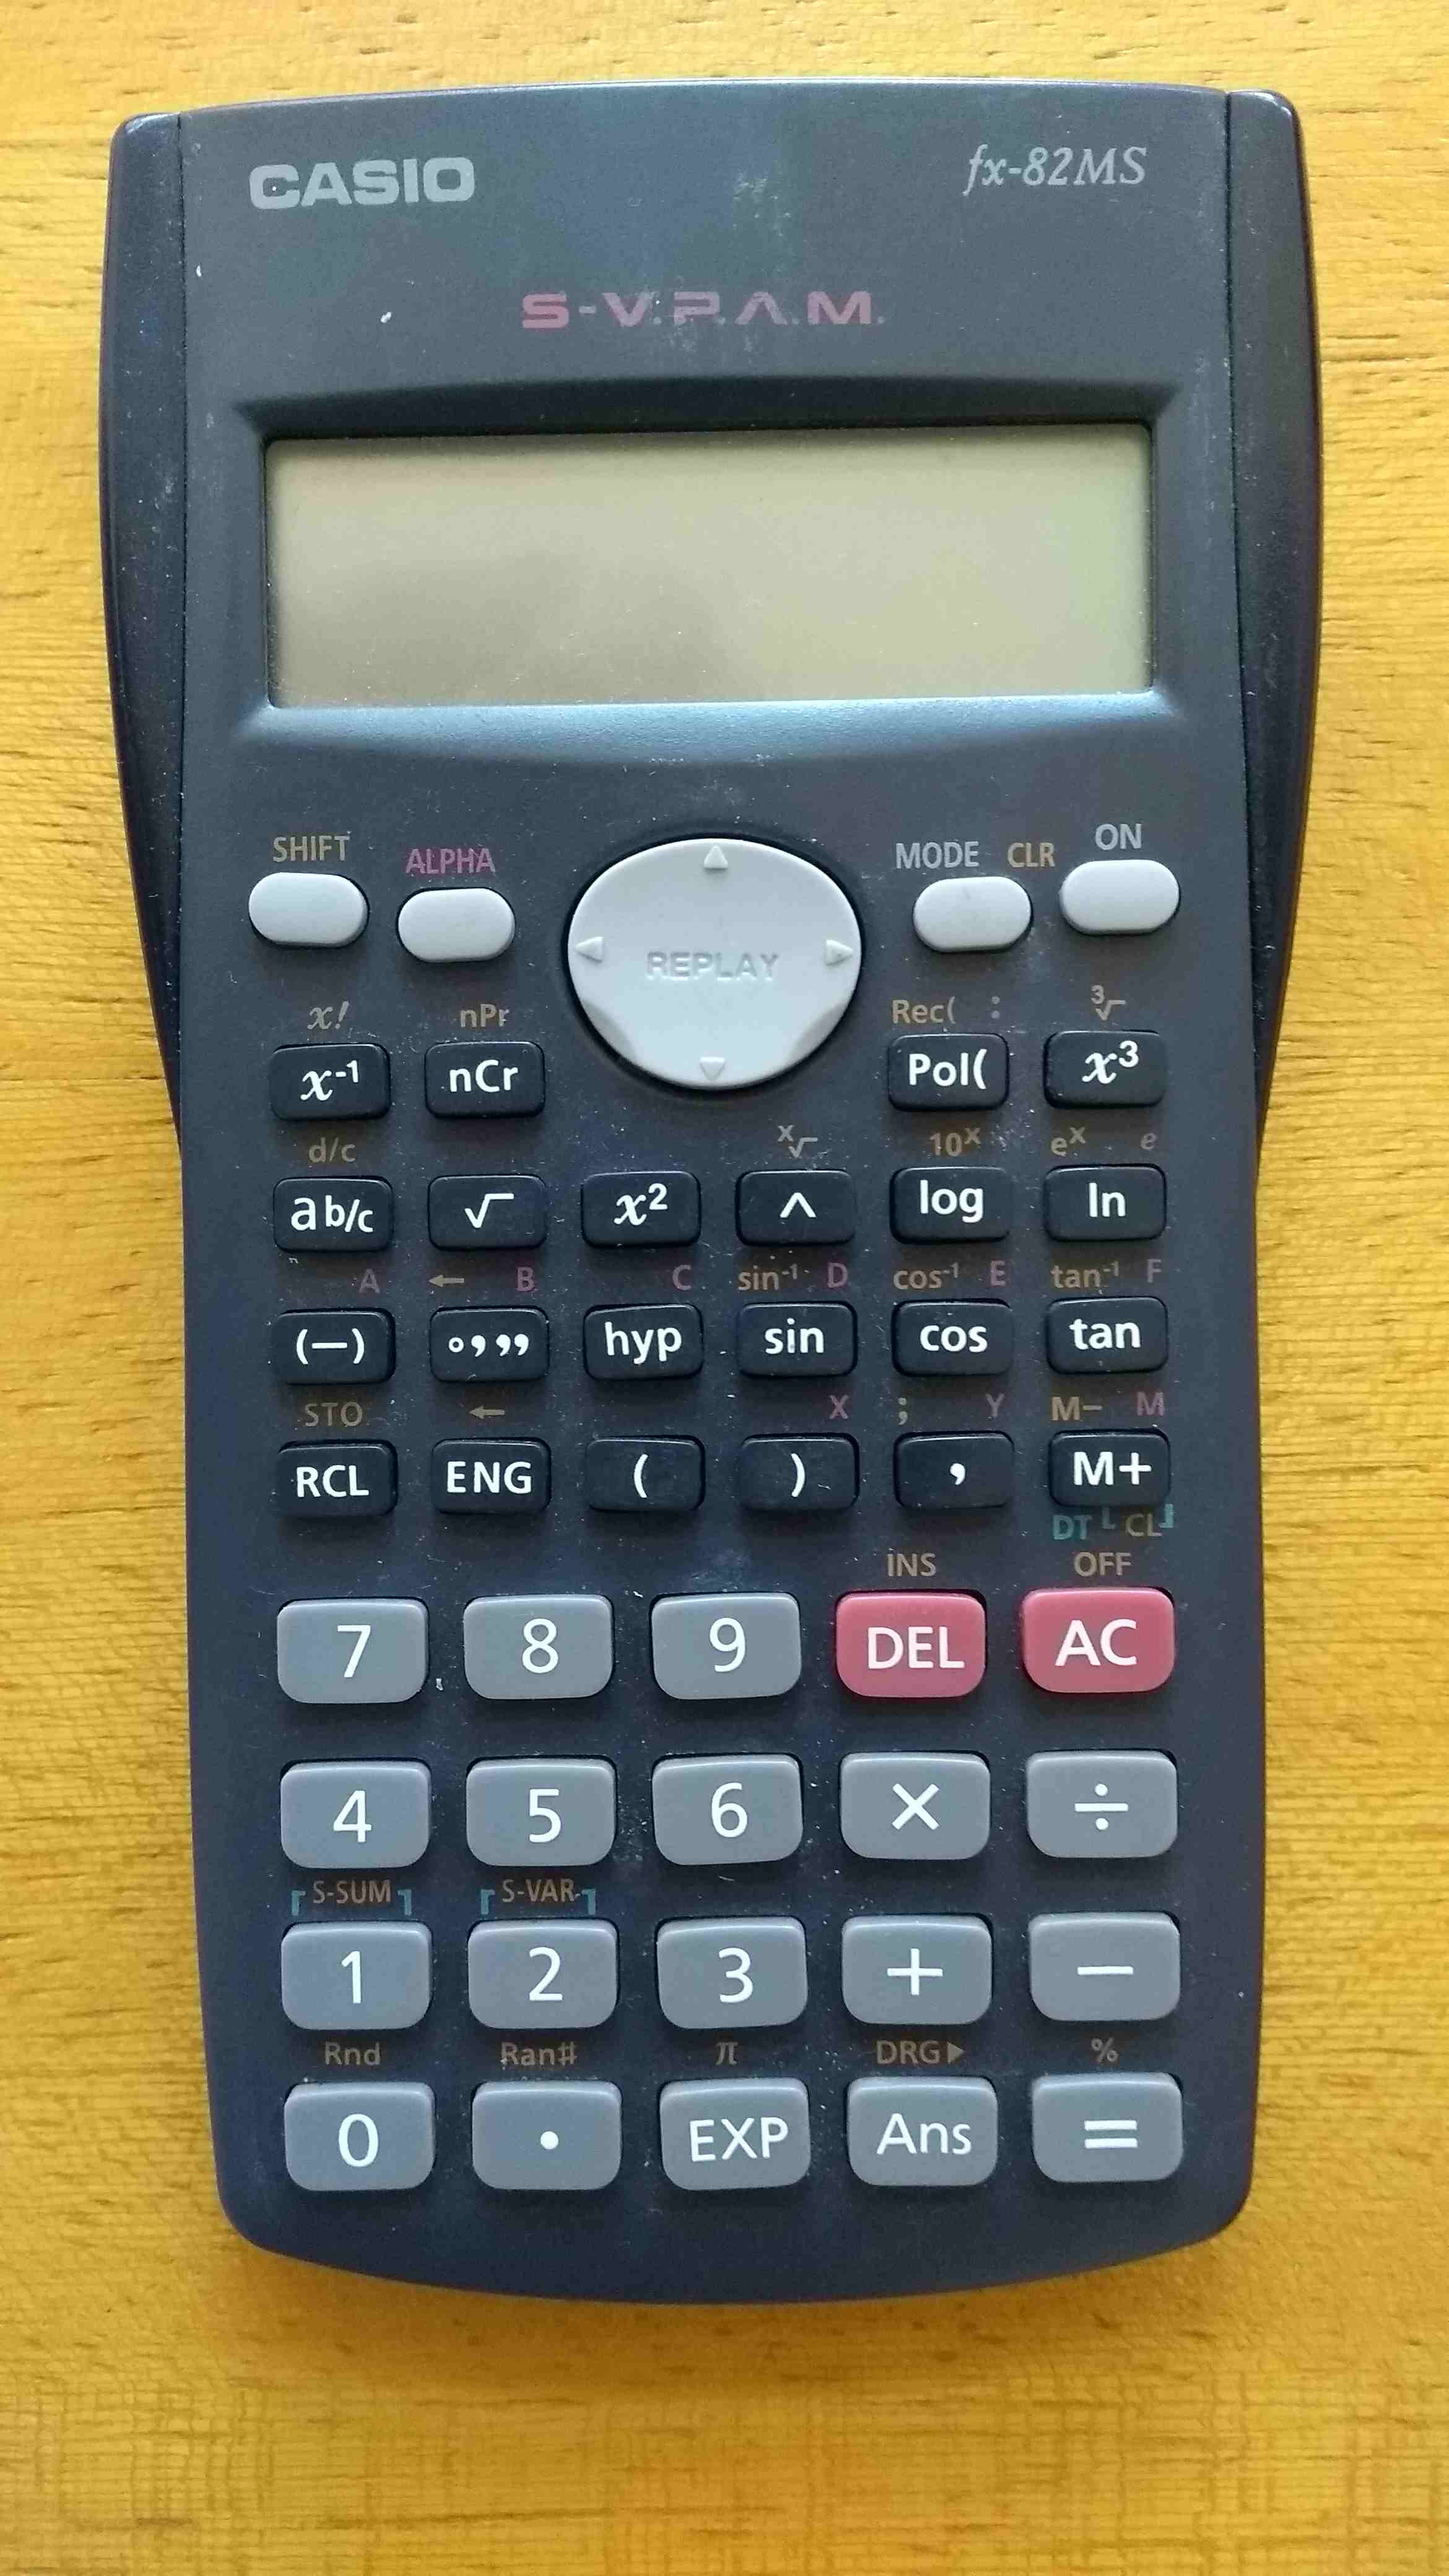
\includegraphics[width=0.8\linewidth]{images2/calculadora_cassio} 

}

\caption{Calculadora Cassio}\label{fig:unnamed-chunk-18}
\end{figure}

\section{Instalação do software R em conjunto com a interface gráfica RStudio}\label{instalauxe7uxe3o-do-software-r-em-conjunto-com-a-interface-gruxe1fica-rstudio}

\hfill\break

\begin{quote}
``A pergunta não é se o R faz; mas sim, como ele faz {[}\ldots{]} (anônimo)''
\end{quote}

\hfill\break

R é uma linguagem e ambiente para computação estatística e gráficos. É um projeto GNU que é semelhante à linguagem e ambiente S que foi desenvolvido nos Laboratórios Bell (anteriormente AT\&T, agora \emph{Lucent Technologies}) por John Chambers e colegas. R pode ser considerado como uma implementação diferente de S. Existem algumas diferenças importantes, mas muito código escrito para S roda inalterado sob R.

R fornece uma ampla variedade de técnicas estatísticas (modelagem linear e não linear, testes estatísticos clássicos, análise de séries temporais, classificação, \emph{clustering}, \ldots) e gráficas, e é altamente extensível. A linguagem S costuma ser o veículo escolhido para pesquisa em metodologia estatística, e R fornece uma rota de código aberto para participação nessa atividade.

Um dos pontos fortes do R é a facilidade com que gráficos de qualidade de publicação bem projetados podem ser produzidos, incluindo símbolos matemáticos e fórmulas quando necessário. Grande cuidado foi tomado sobre os padrões para as escolhas de design menores em gráficos, mas o usuário mantém o controle total.

R está disponível como Software Livre sob os termos da Licença Pública Geral GNU da \emph{Free Software Foundation em} forma de código-fonte. Ele compila e roda em uma ampla variedade de plataformas UNIX e sistemas similares (incluindo FreeBSD e Linux), Windows e MacOS.

R é um conjunto integrado de recursos de software para manipulação de dados, cálculo e exibição gráfica. Inclui:

\begin{itemize}
\tightlist
\item
  uma instalação eficaz de manipulação e armazenamento de dados,
\item
  um conjunto de operadores para cálculos em arrays, em particular matrizes,
  uma coleção grande, coerente e integrada de ferramentas intermediárias para análise de dados,
\item
  facilidades gráficas para análise de dados e exibição na tela ou em cópia impressa, e
  uma linguagem de programação bem desenvolvida, simples e eficaz que inclui condicionais, loops, funções recursivas definidas pelo usuário e recursos de entrada e saída.
\end{itemize}

O termo ``ambiente'' destina-se a caracterizá-lo como um sistema totalmente planejado e coerente, em vez de um acréscimo incremental de ferramentas muito específicas e inflexíveis, como é frequentemente o caso de outros softwares de análise de dados.

R, como S, é projetado em torno de uma verdadeira linguagem de computador e permite aos usuários adicionar funcionalidades adicionais definindo novas funções. Grande parte do sistema é escrito no dialeto R de S, o que torna mais fácil para os usuários seguirem as escolhas algorítmicas feitas. Para tarefas de computação intensiva, os códigos C, C++ e Fortran podem ser vinculados e chamados em tempo de execução. Usuários avançados podem escrever código C para manipular objetos R diretamente.

Muitos usuários pensam no R como um sistema estatístico. Preferimos pensar nisso como um ambiente no qual as técnicas estatísticas são implementadas. R pode ser estendido (facilmente) via packages . Existem cerca de oito pacotes fornecidos com a distribuição R e muitos mais estão disponíveis através da família CRAN de sites da Internet, cobrindo uma ampla gama de estatísticas modernas.

R tem seu próprio formato de documentação semelhante ao LaTeX, que é usado para fornecer documentação abrangente, tanto on-line em vários formatos quanto em cópia impressa.

A página principal pode ser acessa em: \href{https://www.r-project.org/}{The R Project for Statistical Computing} e as informações acima foram traduzidas de \href{https://www.r-project.org/about.html}{Fonte das informações}.

\hfill\break

\subsection{RStudio}\label{rstudio}

\hfill\break

RStudio é um ambiente de desenvolvimento integrado (IDE) para R e Python. Ele inclui um console, editor de realce de sintaxe que oferece suporte à execução direta de código e ferramentas para plotagem, histórico, depuração e gerenciamento de espaço de trabalho. O RStudio está disponível em código aberto e edições comerciais e é executado na área de trabalho (Windows, Mac e Linux). A página principal pode ser acessada em: \href{https://posit.co/download/rstudio-desktop/}{RStudio}.

\hfill\break

Há inúmeros tutoiais para a instalação do \(R\) e o \(RStudio\) (uma IDE: \emph{Integrated development environment} para poder utilizar o software de um mod mais amigável), dentre os quais: \href{http://leg.ufpr.br/~fernandomayer/aulas/ce083-2016-2/R-instalacao.html}{Tutorial de instalação (UFPr)}.

\subsection{Pacotes}\label{pacotes}

\hfill\break

Os pacotes na linguagem de programação R são um conjunto de funções R , código compilado e dados de amostra. Estes são armazenados em um diretório chamado ``biblioteca'' dentro do ambiente R. Por padrão, o R instala um grupo de pacotes durante a instalação. Assim que iniciarmos o console R, apenas os pacotes padrão estarão disponíveis por padrão. Outros pacotes que já estão instalados precisam ser carregados explicitamente para serem utilizados pelo programa R que os usará.

\hfill\break

Uma lista de todos os pacotes disponibilizados para os mais variados problemas de anáise estatística pode ser vista em \href{https://cran.r-project.org/web/packages/available_packages_by_name.html}{Lista de pacotes}.

\hfill\break

\chapter{Introdução à estatística descritiva}\label{introduuxe7uxe3o-uxe0-estatuxedstica-descritiva}

\hfill\break

Sobre o estudo da estatística por áreas nas quais, aparentemente, não se vislumbra sua utilidade trazemos o prefácio da tradução do livro de Jack Levin (Estatística aplicada às ciências humanas) por Sérgio Francisco Costa, ao dizer que o livro:

\hfill\break

\begin{quote}
``{[}\ldots{]} destina-se a um público muito específico: estudantes de Ciências Humanas, refúgio errôneo dos que fogem das equações e dos cálculos, pois que, embora humanas - e talvez por isso mesmo - não podemos prescindir das tão odiadas quantificações {[}\ldots{]}''
\end{quote}

\hfill\break

\section{Análise exploratória}\label{anuxe1lise-exploratuxf3ria}

\hfill\break

A análise exploratória de dados ( \emph{EDA: Exploratory Data Analisys} , originalmente desenvolvida pelo matemático e estatístico norte-americano John Tukey na década de 1970) é usada para se investigar conjuntos de dados e resumir suas principais características, muitas vezes usando métodos de visualização de dados por gráficos e apresentação de tabelas.

\hfill\break

\begin{figure}

{\centering 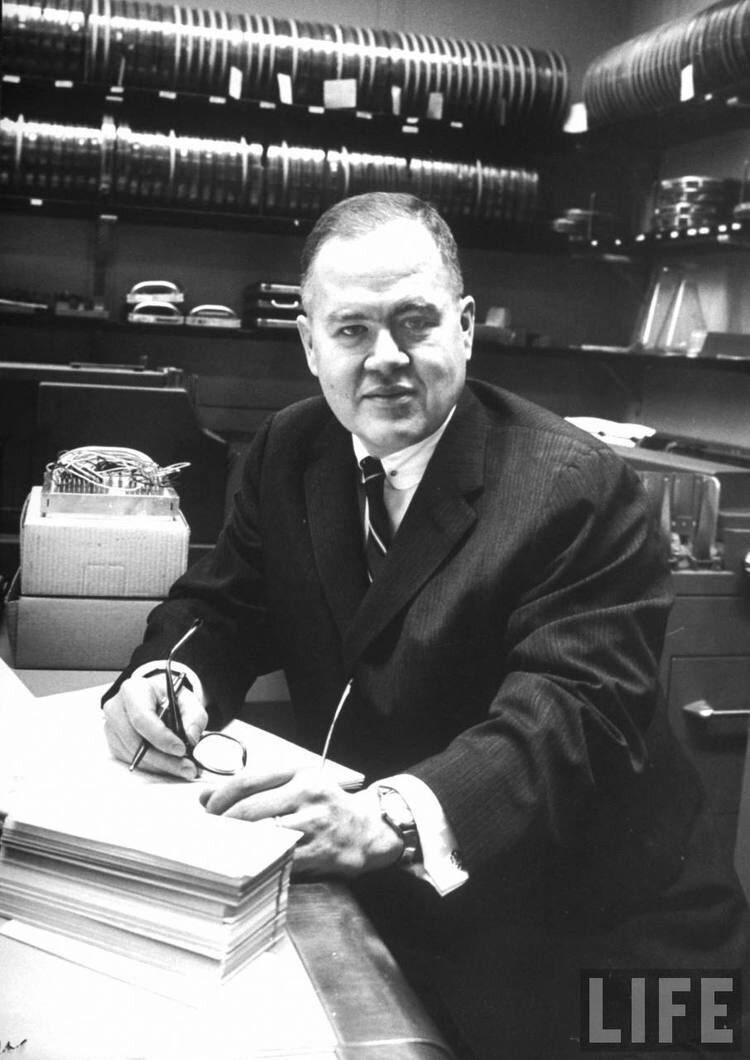
\includegraphics[width=0.5\linewidth]{images3/tukey} 

}

\caption{John Tukey (1915-2000)}\label{fig:unnamed-chunk-21}
\end{figure}

\hfill\break

Habitualmente uma \emph{EDA} envolve:

\begin{itemize}
\tightlist
\item
  verificar quais são os tipos de variáveis presentes nos dados;
\item
  verificar os padrões de cada variável e eventuais associações entre duas ou mais delas; e,
\item
  apresentar os valores assumidos por cada uma das variáveis em formas resumidas como:

  \begin{itemize}
  \tightlist
  \item
    resumos (sínteses) numéricas
  \item
    tabulares e
  \item
    gráficos.
  \end{itemize}
\end{itemize}

\section{Dados brutos, em rol, diagrama de ramos \& folhas e de dispersão unidimensional}\label{dados-brutos-em-rol-diagrama-de-ramos-folhas-e-de-dispersuxe3o-unidimensional}

Consideremos os dados obtidos da medição das alturas em metros de 60 estudantes de uma determinada classe de um certo curso aqui na UEL:

\begin{Shaded}
\begin{Highlighting}[]
\NormalTok{alturas}\OtherTok{=}\FunctionTok{c}\NormalTok{(}\FloatTok{1.63}\NormalTok{,}\FloatTok{1.67}\NormalTok{,}\FloatTok{1.47}\NormalTok{,}\FloatTok{1.64}\NormalTok{,}\FloatTok{1.66}\NormalTok{,}\FloatTok{1.73}\NormalTok{,}\FloatTok{2.00}\NormalTok{,}\FloatTok{1.62}\NormalTok{,}\FloatTok{1.65}\NormalTok{,}\FloatTok{1.56}\NormalTok{,}\FloatTok{1.65}\NormalTok{,}\FloatTok{1.85}\NormalTok{,}\FloatTok{1.73}\NormalTok{,}
          \FloatTok{1.78}\NormalTok{,}\FloatTok{1.82}\NormalTok{,}\FloatTok{1.68}\NormalTok{,}\FloatTok{1.67}\NormalTok{,}\FloatTok{1.83}\NormalTok{,}\FloatTok{1.72}\NormalTok{,}\FloatTok{1.71}\NormalTok{,}\FloatTok{1.73}\NormalTok{,}\FloatTok{1.67}\NormalTok{,}\FloatTok{1.66}\NormalTok{,}\FloatTok{1.95}\NormalTok{,}\FloatTok{1.76}\NormalTok{,}\FloatTok{1.73}\NormalTok{,}
          \FloatTok{1.77}\NormalTok{,}\FloatTok{1.68}\NormalTok{,}\FloatTok{1.65}\NormalTok{,}\FloatTok{1.64}\NormalTok{,}\FloatTok{1.66}\NormalTok{,}\FloatTok{1.68}\NormalTok{,}\FloatTok{1.61}\NormalTok{,}\FloatTok{1.73}\NormalTok{,}\FloatTok{1.72}\NormalTok{,}\FloatTok{1.83}\NormalTok{,}\FloatTok{1.69}\NormalTok{,}\FloatTok{1.84}\NormalTok{,}\FloatTok{1.66}\NormalTok{,}
          \FloatTok{1.78}\NormalTok{,}\FloatTok{1.54}\NormalTok{,}\FloatTok{1.74}\NormalTok{,}\FloatTok{1.56}\NormalTok{,}\FloatTok{1.66}\NormalTok{,}\FloatTok{1.56}\NormalTok{,}\FloatTok{1.62}\NormalTok{,}\FloatTok{1.55}\NormalTok{,}\FloatTok{1.86}\NormalTok{,}\FloatTok{1.44}\NormalTok{,}\FloatTok{1.67}\NormalTok{,}\FloatTok{1.76}\NormalTok{,}\FloatTok{1.79}\NormalTok{,}
          \FloatTok{1.75}\NormalTok{,}\FloatTok{1.41}\NormalTok{,}\FloatTok{1.65}\NormalTok{,}\FloatTok{1.58}\NormalTok{,}\FloatTok{1.93}\NormalTok{,}\FloatTok{1.57}\NormalTok{,}\FloatTok{1.71}\NormalTok{,}\FloatTok{1.58}\NormalTok{,}\FloatTok{0.1}\NormalTok{,}\FloatTok{3.68}\NormalTok{,}\DecValTok{0}\NormalTok{,}\ConstantTok{NA}\NormalTok{)}
\NormalTok{alturas}
\end{Highlighting}
\end{Shaded}

\begin{verbatim}
##  [1] 1.63 1.67 1.47 1.64 1.66 1.73 2.00 1.62 1.65 1.56 1.65 1.85 1.73 1.78 1.82
## [16] 1.68 1.67 1.83 1.72 1.71 1.73 1.67 1.66 1.95 1.76 1.73 1.77 1.68 1.65 1.64
## [31] 1.66 1.68 1.61 1.73 1.72 1.83 1.69 1.84 1.66 1.78 1.54 1.74 1.56 1.66 1.56
## [46] 1.62 1.55 1.86 1.44 1.67 1.76 1.79 1.75 1.41 1.65 1.58 1.93 1.57 1.71 1.58
## [61] 0.10 3.68 0.00   NA
\end{verbatim}

\hfill\break
\emph{Garbage in}, \emph{garbage out}. Não são raras as vezes nas quais o relatório com os dados coletados em uma pesquisa apresentam uma série de erros. Não estamos a nos refeir aqui aos \textbf{erros amostrais} mas sim aos erros experimentais (não amostrais), aqueles decorrentes de dados coletados incorretamente, tais como aqueles resultantes de omissões na transcrição das informações, da leitura de instrumentos descalibrados ou de informações simplesmente não coletadas.

\hfill\break

Denomina-se pré-processamento essa etapa de \emph{limpeza} do conjunto de dados na qual busca-se corrigir de mdo extremamente criterioso esses problemas e, para tanto, um profundo conhecimento do objeto que está sendo pesquisado é necessário de modo a não serem liminarmente eliminados dados simplesmente por destoarem da alguma tendência (para essas tituações há ferramentas estatísticas apropriadas).\\

\hfill\break

O conjunto original de dados ( \emph{dataset}) refere-se a alturas de pessoas (estudantes ) e assim, tata-se de uma variável quantitativa e contínua e como tal será analisada. As omissões de informação ``NA'' ( \emph{not available}) e as medidas transcritas com erros grosseiros (0 m; 0,10 m; 3,68 m) serão removidas.

\hfill\break

Assim, o \emph{dataset} será composto pelos dados abaixo:

\hfill\break

\begin{Shaded}
\begin{Highlighting}[]
\NormalTok{alturas}\OtherTok{=}\FunctionTok{c}\NormalTok{(}\FloatTok{1.63}\NormalTok{,}\FloatTok{1.67}\NormalTok{,}\FloatTok{1.47}\NormalTok{,}\FloatTok{1.64}\NormalTok{,}\FloatTok{1.66}\NormalTok{,}\FloatTok{1.73}\NormalTok{,}\FloatTok{2.00}\NormalTok{,}\FloatTok{1.62}\NormalTok{,}\FloatTok{1.65}\NormalTok{,}\FloatTok{1.56}\NormalTok{,}\FloatTok{1.65}\NormalTok{,}\FloatTok{1.85}\NormalTok{,}\FloatTok{1.73}\NormalTok{,}
          \FloatTok{1.78}\NormalTok{,}\FloatTok{1.82}\NormalTok{,}\FloatTok{1.68}\NormalTok{,}\FloatTok{1.67}\NormalTok{,}\FloatTok{1.83}\NormalTok{,}\FloatTok{1.72}\NormalTok{,}\FloatTok{1.71}\NormalTok{,}\FloatTok{1.73}\NormalTok{,}\FloatTok{1.67}\NormalTok{,}\FloatTok{1.66}\NormalTok{,}\FloatTok{1.95}\NormalTok{,}\FloatTok{1.76}\NormalTok{,}\FloatTok{1.73}\NormalTok{,}
          \FloatTok{1.77}\NormalTok{,}\FloatTok{1.68}\NormalTok{,}\FloatTok{1.65}\NormalTok{,}\FloatTok{1.64}\NormalTok{,}\FloatTok{1.66}\NormalTok{,}\FloatTok{1.68}\NormalTok{,}\FloatTok{1.61}\NormalTok{,}\FloatTok{1.73}\NormalTok{,}\FloatTok{1.72}\NormalTok{,}\FloatTok{1.83}\NormalTok{,}\FloatTok{1.69}\NormalTok{,}\FloatTok{1.84}\NormalTok{,}\FloatTok{1.66}\NormalTok{,}
          \FloatTok{1.78}\NormalTok{,}\FloatTok{1.54}\NormalTok{,}\FloatTok{1.74}\NormalTok{,}\FloatTok{1.56}\NormalTok{,}\FloatTok{1.66}\NormalTok{,}\FloatTok{1.56}\NormalTok{,}\FloatTok{1.62}\NormalTok{,}\FloatTok{1.55}\NormalTok{,}\FloatTok{1.86}\NormalTok{,}\FloatTok{1.44}\NormalTok{,}\FloatTok{1.67}\NormalTok{,}\FloatTok{1.76}\NormalTok{,}\FloatTok{1.79}\NormalTok{,}
          \FloatTok{1.75}\NormalTok{,}\FloatTok{1.41}\NormalTok{,}\FloatTok{1.65}\NormalTok{,}\FloatTok{1.58}\NormalTok{,}\FloatTok{1.93}\NormalTok{,}\FloatTok{1.57}\NormalTok{,}\FloatTok{1.71}\NormalTok{,}\FloatTok{1.58}\NormalTok{)}
\NormalTok{alturas}
\end{Highlighting}
\end{Shaded}

\begin{verbatim}
##  [1] 1.63 1.67 1.47 1.64 1.66 1.73 2.00 1.62 1.65 1.56 1.65 1.85 1.73 1.78 1.82
## [16] 1.68 1.67 1.83 1.72 1.71 1.73 1.67 1.66 1.95 1.76 1.73 1.77 1.68 1.65 1.64
## [31] 1.66 1.68 1.61 1.73 1.72 1.83 1.69 1.84 1.66 1.78 1.54 1.74 1.56 1.66 1.56
## [46] 1.62 1.55 1.86 1.44 1.67 1.76 1.79 1.75 1.41 1.65 1.58 1.93 1.57 1.71 1.58
\end{verbatim}

\hfill\break

Esse conjunto de dados certamente contém diversas informações acerca da altura dessas pessoas; todavia, da maneira como estão expostos, a visualização dessas informações fica bastante difícil. Esse modo de apresentação é chamado de dados \emph{brutos}.

\hfill\break

Com um pequeno refinamento, como pela simples ordenação desses dados (são medidas numéricas contínuas), algumas informações começam a se destacar:

\hfill\break

\begin{Shaded}
\begin{Highlighting}[]
\FunctionTok{sort}\NormalTok{(alturas)}
\end{Highlighting}
\end{Shaded}

\begin{verbatim}
##  [1] 1.41 1.44 1.47 1.54 1.55 1.56 1.56 1.56 1.57 1.58 1.58 1.61 1.62 1.62 1.63
## [16] 1.64 1.64 1.65 1.65 1.65 1.65 1.66 1.66 1.66 1.66 1.66 1.67 1.67 1.67 1.67
## [31] 1.68 1.68 1.68 1.69 1.71 1.71 1.72 1.72 1.73 1.73 1.73 1.73 1.73 1.74 1.75
## [46] 1.76 1.76 1.77 1.78 1.78 1.79 1.82 1.83 1.83 1.84 1.85 1.86 1.93 1.95 2.00
\end{verbatim}

\hfill\break

A interpretabilidade das informações trazidas por esses dados começa a ficar mais fácil como, por exemplo, as alturas:

\hfill\break

\begin{itemize}
\tightlist
\item
  mínima; e,
\item
  máxima dos estudantes.
\end{itemize}

\hfill\break

A uma listagem de valores ordenada (de modo crescente ou decrescente) dá-se o nome de \emph{rol}.

\hfill\break

Outra forma de apresentação desses dados é por um \emph{Diagrama de Ramos e Folhas}, uma apresentação híbrida pois ao mesmo tempo que espelha a quantidade de medidas observadas para cada altura, mantém as informações da listagem.

\hfill\break

\begin{Shaded}
\begin{Highlighting}[]
\FunctionTok{stem}\NormalTok{(alturas)}
\end{Highlighting}
\end{Shaded}

\begin{verbatim}
## 
##   The decimal point is 1 digit(s) to the left of the |
## 
##   14 | 147
##   15 | 45666788
##   16 | 12234455556666677778889
##   17 | 11223333345667889
##   18 | 233456
##   19 | 35
##   20 | 0
\end{verbatim}

\hfill\break

À esquerda do traço vertical (os ramos) são apresentadas frações das medidas das alturas (no caso, decímetros) e à direita (as folhas) são apresentadas os complementos dessas medidas (os centímetros) de tal modo que cada um dos dados da amostral original possa ter sua medida resgatada fazendo-se a leitura dos valores à esquerda com cada um deles à direita.

\hfill\break

Essa apresentação também oferece uma apreciação visual a respeito de como os valores se distribuem.

\hfill\break

Um \emph{Gráfico de dispersão unidimensional (stripchart)} expressa visualmente duas informações: a localização de cada uma das medidas e a dispersão dos dados.

\hfill\break

\begin{Shaded}
\begin{Highlighting}[]
\FunctionTok{stripchart}\NormalTok{(alturas, }\AttributeTok{method =} \StringTok{"stack"}\NormalTok{, }\AttributeTok{offset=}\DecValTok{1}\NormalTok{,}
           \AttributeTok{pch=}\DecValTok{20}\NormalTok{, }\AttributeTok{at=}\FloatTok{0.5}\NormalTok{,}
           \AttributeTok{main=}\StringTok{"Gráfico de dispersão unidimensional"}\NormalTok{,}
           \AttributeTok{col=}\StringTok{"blue"}\NormalTok{,}\AttributeTok{cex=}\DecValTok{1}\NormalTok{,}
           \AttributeTok{xlab=}\StringTok{"Alturas dos estudantes (m)"}\NormalTok{,}
           \AttributeTok{ylab=}\StringTok{"Quantidades observadas (un)"}\NormalTok{)}
\end{Highlighting}
\end{Shaded}

\begin{figure}

{\centering 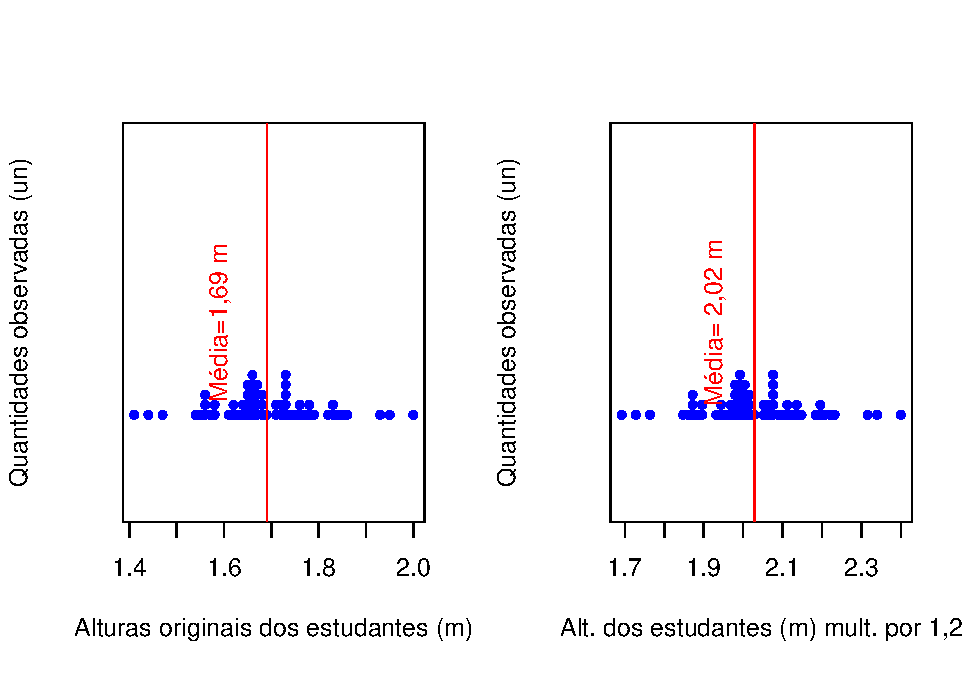
\includegraphics[width=0.8\linewidth]{apostila_files/figure-latex/unnamed-chunk-26-1} 

}

\caption{Gráfico de dispersão unidimensional (stripchart)}\label{fig:unnamed-chunk-26}
\end{figure}

\section{Resumos (sínteses) numéricos descritivos}\label{resumos-suxednteses-numuxe9ricos-descritivos}

\hfill\break

Além da apresentação elementar de algumas informações relacionadas aos dados brutos da amostra, tais como os valores \emph{mínimo} e \emph{máximo} observados, a estatística descritiva possui muitas outras ferramentas para \emph{condensar} a informação trazida pelos dados.

\hfill\break

São chamadas de \emph{sínteses numéricas}, medidas que condensam variados aspectos relacionados aos valores dos dados.

\hfill\break

As mais conhecidas \emph{sínteses numéricas} podem ser agrupadas conforme o aspecto que capturam dos dados:

\hfill\break

\begin{itemize}
\tightlist
\item
  tendência central (posição): média (simples ou aritmética, geométrica, harmônica, anarmônica, quadrática, biquadrática), moda e mediana;
\item
  dispersão (variabilidade): absolutas (amplitude total, variância e desvio padrão) ou relativas (coeficiente de variação, unidades padronizadas); e,
\item
  subdivisão (separatrizes, quantis): mediana (50\%), quartis (25\%, 50\%, 75\%), decis (10\%, \ldots.90\%) e percentis (1\%\ldots.99\%).
\end{itemize}

\hfill\break

Uma medida de posição ou dispersão é dita \textbf{resistente} quando forem pouco afetadas pela alteração de uma pequena porção dos dados. A mediana é uma medida resistente, já a média e a variância não são.

\subsection{Medidas de tendência central (posição)}\label{medidas-de-tenduxeancia-central-posiuxe7uxe3o}

\subsubsection{Média}\label{muxe9dia}

\hfill\break

Sejam \(x_{1}, x_{2}, ..., x_{n}\) os \(n\) valores assumidos pela variável \(X\) (dados brutos). A \emph{média aritmética simples} será dada por:

\hfill\break

\[
\stackrel{-}{x}=\frac{\sum _{i=1}^{n}{x}_{i}}{n}
\]

\hfill\break

Algumas propriedades da média aritmética:

\hfill\break

\begin{itemize}
\tightlist
\item
  somando-se (ou subtraindo-se) cada um dos elementos do conjunto de dados por uma constante arbitrária qualquer \(k\), a média aritmética ficará adicionada (ou subtraída) dessa essa constante \(k\)
\end{itemize}

\hfill\break

\begin{Shaded}
\begin{Highlighting}[]
\NormalTok{alturas\_ad}\OtherTok{=}\NormalTok{alturas}\FloatTok{+0.05}

\FunctionTok{par}\NormalTok{(}\AttributeTok{mfrow=}\FunctionTok{c}\NormalTok{(}\DecValTok{1}\NormalTok{,}\DecValTok{2}\NormalTok{))}

\FunctionTok{stripchart}\NormalTok{(alturas,}\AttributeTok{method =} \StringTok{"stack"}\NormalTok{,  }\AttributeTok{at=}\FloatTok{0.5}\NormalTok{, }
\AttributeTok{main=}\StringTok{""}\NormalTok{,}\AttributeTok{pch =} \DecValTok{20}\NormalTok{,}
\AttributeTok{col=}\StringTok{"blue"}\NormalTok{, }\AttributeTok{cex=}\DecValTok{1}\NormalTok{, }\AttributeTok{xlab=}\StringTok{"Alturas originais dos estudantes (m)"}\NormalTok{, }
\AttributeTok{ylab=}\StringTok{"Quantidades observadas (un)"}\NormalTok{)}
\FunctionTok{abline}\NormalTok{(}\AttributeTok{v=}\FunctionTok{mean}\NormalTok{(alturas), }\AttributeTok{col=}\StringTok{"red"}\NormalTok{) }
\FunctionTok{text}\NormalTok{(}\FunctionTok{mean}\NormalTok{(alturas)}\SpecialCharTok{{-}}\FloatTok{0.2}\NormalTok{, }\DecValTok{1}\NormalTok{, }\StringTok{"Média=1,69 m"}\NormalTok{, }\AttributeTok{col =} \StringTok{"red"}\NormalTok{, }\AttributeTok{srt=}\DecValTok{90}\NormalTok{) }

\FunctionTok{stripchart}\NormalTok{(alturas\_ad,}\AttributeTok{method =} \StringTok{"stack"}\NormalTok{,  }\AttributeTok{at=}\FloatTok{0.5}\NormalTok{, }
\AttributeTok{main=}\StringTok{""}\NormalTok{,}\AttributeTok{pch =} \DecValTok{20}\NormalTok{,}
\AttributeTok{col=}\StringTok{"blue"}\NormalTok{, }\AttributeTok{cex=}\DecValTok{1}\NormalTok{, }\AttributeTok{xlab=}\StringTok{"Alt. dos estudantes (m) adic. de 5cm"}\NormalTok{, }
\AttributeTok{ylab=}\StringTok{"Quantidades observadas (un)"}\NormalTok{)}
\FunctionTok{abline}\NormalTok{(}\AttributeTok{v=}\FunctionTok{mean}\NormalTok{(alturas\_ad), }\AttributeTok{col=}\StringTok{"red"}\NormalTok{) }
\FunctionTok{text}\NormalTok{(}\FunctionTok{mean}\NormalTok{(alturas\_ad)}\SpecialCharTok{{-}}\FloatTok{0.2}\NormalTok{, }\DecValTok{1}\NormalTok{, }\StringTok{"Média=1,74 m"}\NormalTok{, }\AttributeTok{col =} \StringTok{"red"}\NormalTok{, }\AttributeTok{srt=}\DecValTok{90}\NormalTok{) }
\end{Highlighting}
\end{Shaded}

\begin{figure}

{\centering 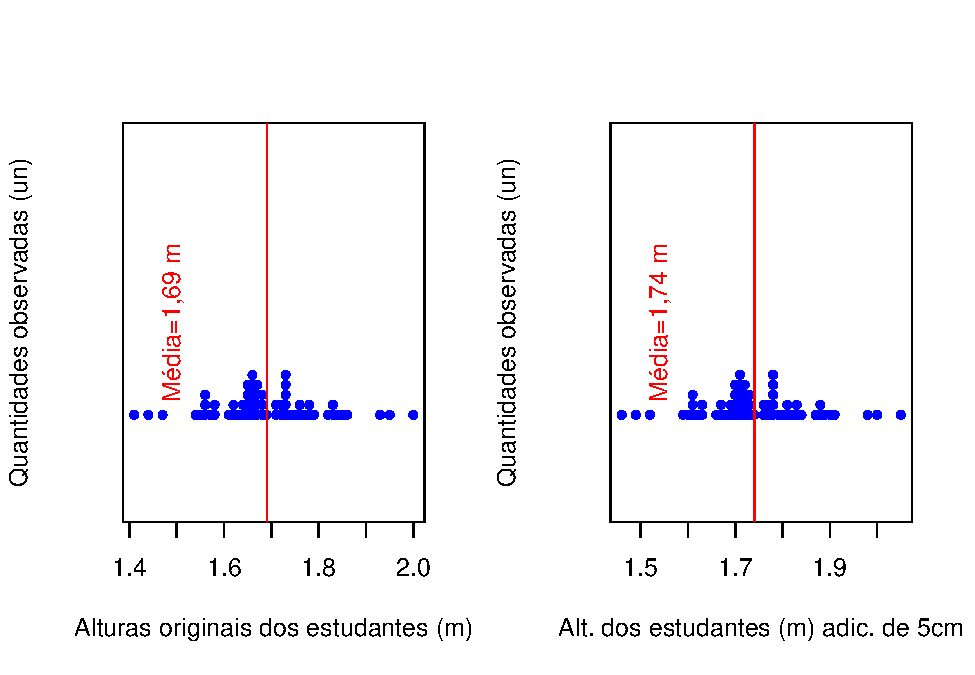
\includegraphics[width=0.8\linewidth]{apostila_files/figure-latex/unnamed-chunk-27-1} 

}

\caption{Mudanças na média pela adição (subtração) de uma constante $k=0.05$}\label{fig:unnamed-chunk-27}
\end{figure}

\hfill\break

\begin{itemize}
\tightlist
\item
  multiplicando-se (ou dividindo-se) cada um dos elementos do conjunto de dados por uma constante arbitrária \(k\), a média aritmética ficará multiplicada (ou dividida) por essa constante \(k\)
\end{itemize}

\hfill\break

\begin{Shaded}
\begin{Highlighting}[]
\NormalTok{alturas\_mult}\OtherTok{=}\NormalTok{alturas}\SpecialCharTok{*}\FloatTok{1.2}

\FunctionTok{par}\NormalTok{(}\AttributeTok{mfrow=}\FunctionTok{c}\NormalTok{(}\DecValTok{1}\NormalTok{,}\DecValTok{2}\NormalTok{))}

\FunctionTok{stripchart}\NormalTok{(alturas,}\AttributeTok{method =} \StringTok{"stack"}\NormalTok{,  }\AttributeTok{at=}\FloatTok{0.5}\NormalTok{, }
\AttributeTok{main=}\StringTok{""}\NormalTok{,}\AttributeTok{pch =} \DecValTok{20}\NormalTok{,}
\AttributeTok{col=}\StringTok{"blue"}\NormalTok{,  }\AttributeTok{xlab=}\StringTok{"Alturas originais dos estudantes (m)"}\NormalTok{, }
\AttributeTok{ylab=}\StringTok{"Quantidades observadas (un)"}\NormalTok{)}
\FunctionTok{abline}\NormalTok{(}\AttributeTok{v=}\FunctionTok{mean}\NormalTok{(alturas), }\AttributeTok{col=}\StringTok{"red"}\NormalTok{) }
\FunctionTok{text}\NormalTok{(}\FunctionTok{mean}\NormalTok{(alturas)}\SpecialCharTok{{-}}\FloatTok{0.1}\NormalTok{, }\DecValTok{1}\NormalTok{, }\StringTok{"Média=1,69 m"}\NormalTok{, }\AttributeTok{col =} \StringTok{"red"}\NormalTok{, }\AttributeTok{srt=}\DecValTok{90}\NormalTok{) }


\FunctionTok{stripchart}\NormalTok{(alturas\_mult,}\AttributeTok{method =} \StringTok{"stack"}\NormalTok{,  }\AttributeTok{at=}\FloatTok{0.5}\NormalTok{, }
\AttributeTok{main=}\StringTok{""}\NormalTok{,}\AttributeTok{pch =} \DecValTok{20}\NormalTok{,}
\AttributeTok{col=}\StringTok{"blue"}\NormalTok{,  }\AttributeTok{xlab=}\StringTok{"Alt. dos estudantes (m) mult. por 1,2"}\NormalTok{, }
\AttributeTok{ylab=}\StringTok{"Quantidades observadas (un)"}\NormalTok{)}
\FunctionTok{abline}\NormalTok{(}\AttributeTok{v=}\FunctionTok{mean}\NormalTok{(alturas\_mult), }\AttributeTok{col=}\StringTok{"red"}\NormalTok{) }
\FunctionTok{text}\NormalTok{(}\FunctionTok{mean}\NormalTok{(alturas\_mult)}\SpecialCharTok{{-}}\FloatTok{0.1}\NormalTok{, }\DecValTok{1}\NormalTok{, }\StringTok{"Média= 2,02 m"}\NormalTok{, }\AttributeTok{col =} \StringTok{"red"}\NormalTok{, }\AttributeTok{srt=}\DecValTok{90}\NormalTok{) }
\end{Highlighting}
\end{Shaded}

\begin{figure}

{\centering 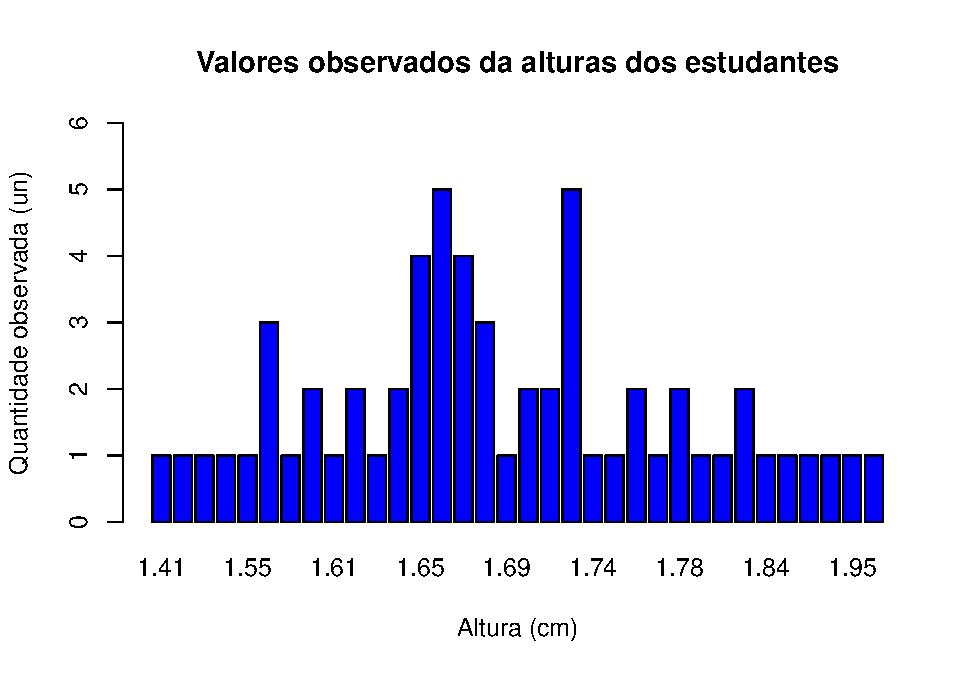
\includegraphics[width=0.8\linewidth]{apostila_files/figure-latex/unnamed-chunk-28-1} 

}

\caption{Mudanças na média pela multiplicação (divisão) de uma constante $k=1.2$}\label{fig:unnamed-chunk-28}
\end{figure}

\hfill\break

\begin{itemize}
\tightlist
\item
  a soma dos desvios observados entre cada um dos valores assumidos pela variável \(X\) e sua média \(\stackrel{-}{x}\) é nula;
\item
  a soma dos quadrados dos desvios é mínima;
\item
  em uma distribuição de frequências, a soma dos produtos dos desvios entre a média o valor médio de cada uma das classes, pelas respectivas frequências é nula; e,
\item
  multiplicando-se (ou dividindo-se) todas as frequências de uma distribuição por uma constante arbitrária, a média aritmética não se altera.
\end{itemize}

\hfill\break

Usando os dados das medidas das alturas dos 60 estudantes teremos o seguinte valor para a \textbf{média}:

\hfill\break

\begin{Shaded}
\begin{Highlighting}[]
\FunctionTok{round}\NormalTok{(}\FunctionTok{mean}\NormalTok{(alturas),}\DecValTok{2}\NormalTok{)}
\end{Highlighting}
\end{Shaded}

\begin{verbatim}
## [1] 1.69
\end{verbatim}

\subsubsection{Moda}\label{moda}

\hfill\break

Moda é o valor que ocorre com maior frequência na amostra. Uma amostra pode se apresentar como:

\hfill\break

\begin{itemize}
\tightlist
\item
  unimodal;
\item
  bimodal;
\item
  plurimodal; ou,
\item
  amodal.
\end{itemize}

\hfill\break

\begin{Shaded}
\begin{Highlighting}[]
\NormalTok{tab\_alturas}\OtherTok{=}\FunctionTok{table}\NormalTok{(alturas)}

\NormalTok{tab\_alturas}
\end{Highlighting}
\end{Shaded}

\begin{verbatim}
## alturas
## 1.41 1.44 1.47 1.54 1.55 1.56 1.57 1.58 1.61 1.62 1.63 1.64 1.65 1.66 1.67 1.68 
##    1    1    1    1    1    3    1    2    1    2    1    2    4    5    4    3 
## 1.69 1.71 1.72 1.73 1.74 1.75 1.76 1.77 1.78 1.79 1.82 1.83 1.84 1.85 1.86 1.93 
##    1    2    2    5    1    1    2    1    2    1    1    2    1    1    1    1 
## 1.95    2 
##    1    1
\end{verbatim}

\begin{Shaded}
\begin{Highlighting}[]
\FunctionTok{barplot}\NormalTok{(tab\_alturas,}
        \AttributeTok{main=}\StringTok{"Valores observados da alturas dos estudantes"}\NormalTok{,}
        \AttributeTok{xlab=}\StringTok{"Altura (cm)"}\NormalTok{,}
        \AttributeTok{ylab=}\StringTok{"Quantidade observada (un)"}\NormalTok{,}
        \AttributeTok{ylim=}\FunctionTok{c}\NormalTok{(}\DecValTok{0}\NormalTok{,}\DecValTok{6}\NormalTok{),}
        \AttributeTok{col=}\StringTok{"blue"}\NormalTok{,}
        \AttributeTok{las=}\DecValTok{0}\NormalTok{, }
        \AttributeTok{hor=}\StringTok{"FALSE"}\NormalTok{)}
\end{Highlighting}
\end{Shaded}

\begin{figure}
\centering
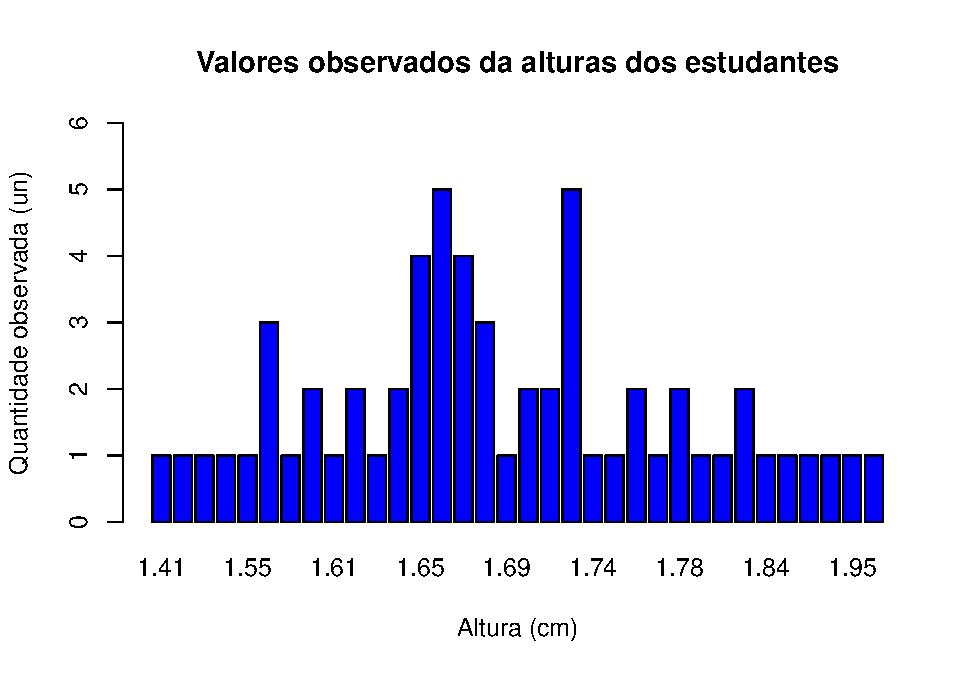
\includegraphics{apostila_files/figure-latex/unnamed-chunk-30-1.pdf}
\caption{\label{fig:unnamed-chunk-30}Bimodal: 1,66 m e 1,73 m}
\end{figure}

\hfill\break

Usando os dados das medidas das alturas dos 60 estudantes teremos os seguintes valores para a \textbf{moda}:

\hfill\break

\begin{Shaded}
\begin{Highlighting}[]
\CommentTok{\# função em R para extrair a moda:}

\NormalTok{Modes }\OtherTok{\textless{}{-}} \ControlFlowTok{function}\NormalTok{(x) \{}
\NormalTok{  ux }\OtherTok{\textless{}{-}} \FunctionTok{unique}\NormalTok{(x)}
\NormalTok{  tab }\OtherTok{\textless{}{-}} \FunctionTok{tabulate}\NormalTok{(}\FunctionTok{match}\NormalTok{(x, ux))}
\NormalTok{  ux[tab }\SpecialCharTok{==} \FunctionTok{max}\NormalTok{(tab)]}
\NormalTok{\}}

\FunctionTok{Modes}\NormalTok{(alturas)}
\end{Highlighting}
\end{Shaded}

\begin{verbatim}
## [1] 1.66 1.73
\end{verbatim}

\subsection{Medidas de dispersão (variabilidade)}\label{medidas-de-dispersuxe3o-variabilidade}

\hfill\break

O conhecimento de uma medida de tendência central nos provê uma informação útil mas incompleta. As medidas de dispersão nos ajudam a ter uma perspectiva melhor dos dados.

\hfill\break

\begin{itemize}
\tightlist
\item
  amplitude total dos dados;
\item
  desvio padrão (variância): é considerada a mais útil das medidas de dispersão;\\
\item
  coeficiente de variação; e,
\item
  unidades padronizadas.
\end{itemize}

\hfill\break

Diferentes tipos quanto à dimensão (unidade):

\hfill\break

\begin{itemize}
\tightlist
\item
  \textbf{medidas absolutas} são aquelas expressas na mesma unidade de medida da variável do fenômeno estudado (\(m;kg;\frac{R\$}{mês};\dots\));\\
\item
  \textbf{medidas relativas} são adimiensionais e assim podem ser usadas para se comparar a variabilidade de dois ou mais conjuntos de dados, mesmo quando as variáveis se refiram a diferentes fenômenos ou que sejam expressas, originalmente, em diferentes unidades.
\end{itemize}

\hfill\break

\subsubsection{Amplitude total dos dados}\label{amplitude-total-dos-dados}

\hfill\break

A amplitude total dos dados é a simples diferença entre o \textbf{maior} e o \textbf{menor} dos valores observados:

\hfill\break

\[
A=x_{max} - x_{min}
\]

\hfill\break

\subsubsection{Variância (e desvio padrão)}\label{variuxe2ncia-e-desvio-padruxe3o}

\hfill\break

Sejam \(x_{1}, x_{2}, ..., x_{n}\) os \(n\) valores assumidos pela variável \(X\). Dá-se o nome de desvios a contar da média as diferenças entre cada uma das observações e a média: \(x_{i} - \stackrel{-}{x}\) com \(i=1,2,...,n\).

\hfill\break

Não é possível considerar a possibilidade de se adotar o valor médio desses desvios pois uma das propriedades da média é que a soma dos desvios em torno de si é nula.

\hfill\break

\[
\stackrel{-}{d} = \frac{\sum _{i=1}^{n}\left(x_{i}-\stackrel{-}{x}\right)}{n}
\]
\[
\sum _{i=1}^{n}\left(x_{i}-\stackrel{-}{x}\right)=0
\]

\hfill\break

constitui-se numa restrição linear dos desvios porque qualquer \(n-1\) deles completamente determina o outro. Tampouco se considera a possibilidade de se adotar o valor médio desses desvios em módulo, pelas dificuldades teóricas em problemas de inferência.

\hfill\break

\[
\stackrel{-}{d}  = \frac{\sum _{i=1}^{n}\left|x_{i}-\stackrel{-}{x}\right|}{n}
\]

\hfill\break

Uma alternativa é adotar o valor médio do \textbf{quadrado} desses desvios.

\hfill\break

\[
S^{2}=\frac{\sum _{i=1}^{n}\left(x_{i}-\stackrel{-}{x}\right)^{2}}{n-1}
\]

\hfill\break

ou,

\hfill\break

\[
S^{2}=\frac{1}{(n-1)} \times \left[ \sum _{i=1}^{n} (x_{i}^{2}) - \frac{({\sum _{i=1}^{n}x_{i})}^{2} }{n}\right]
\]

\hfill\break

Diz-se que a variância amostral (variância \emph{ajustada}) possui \((n-1)\) graus de liberdade, denotado pela letra grega \(\nu\). A perda de \emph{um} grau de liberdade deve-se à necessidade de se substituir a média populacional desconhecida (\(\mu\)) por sua estimativa amostral (\(\stackrel{-}{x}\)), deduzida a partir dos dados coletados.

\hfill\break

Pode-se demonstrar que em razão dessa restrição a melhor estimativa para a variância populacional é obtida dividindo-se a soma dos quadrados dos desvios por \((n-1)\). Assim \(S^{2}\) será um estimador não tendencioso para a variância amostral ao ser dividido por \((n-1)\).

\hfill\break

\begin{Shaded}
\begin{Highlighting}[]
\NormalTok{IC.Na }\OtherTok{=} \ControlFlowTok{function}\NormalTok{ (N, n, mu, sigma) \{}
\NormalTok{  dados}\OtherTok{=}\FunctionTok{data.frame}\NormalTok{()}
  \FunctionTok{plot}\NormalTok{(}\DecValTok{0}\NormalTok{, }\DecValTok{0}\NormalTok{, }
       \AttributeTok{type=}\StringTok{"n"}\NormalTok{, }
       \AttributeTok{xlim=}\FunctionTok{c}\NormalTok{(sigma}\FloatTok{{-}0.1}\SpecialCharTok{*}\NormalTok{sigma,sigma}\FloatTok{+0.1}\SpecialCharTok{*}\NormalTok{sigma), }
       \AttributeTok{ylim=}\FunctionTok{c}\NormalTok{(}\DecValTok{0}\NormalTok{,N), }
       \AttributeTok{bty=}\StringTok{"l"}\NormalTok{,}
       \AttributeTok{xlab=}\StringTok{"Desvio padrão"}\NormalTok{, }
       \AttributeTok{ylab=}\StringTok{"Amostras extraídas"}\NormalTok{, }
       \AttributeTok{main=}\FunctionTok{paste0}\NormalTok{(}\StringTok{"Flutuação dos valores dos desvios padrão }\SpecialCharTok{\textbackslash{}n}\StringTok{obtidos em "}\NormalTok{, N,}\StringTok{" amostras de tamanho "}\NormalTok{,n), }
       \AttributeTok{sub=}\FunctionTok{paste0}\NormalTok{(}\StringTok{"A população de origem tem uma distribuição \textasciitilde{} N  (\textbackslash{}u03bc:"}\NormalTok{,mu,}\StringTok{" ; \textbackslash{}u03c3:"}\NormalTok{, sigma,}\StringTok{")"}\NormalTok{))}
  \FunctionTok{abline}\NormalTok{(}\AttributeTok{v=}\NormalTok{sigma, }\AttributeTok{col=}\StringTok{\textquotesingle{}darkgreen\textquotesingle{}}\NormalTok{, }\AttributeTok{lwd=}\DecValTok{2}\NormalTok{, }\AttributeTok{lty=}\DecValTok{2}\NormalTok{)}
\ControlFlowTok{for}\NormalTok{ (i }\ControlFlowTok{in} \DecValTok{1}\SpecialCharTok{:}\NormalTok{N) \{}
\NormalTok{  x }\OtherTok{=} \FunctionTok{rnorm}\NormalTok{(n, mu, sigma)}
\NormalTok{  media }\OtherTok{=} \FunctionTok{mean}\NormalTok{(x)}
\NormalTok{  sd }\OtherTok{=} \FunctionTok{sqrt}\NormalTok{(}\FunctionTok{sum}\NormalTok{((x}\SpecialCharTok{{-}}\FunctionTok{mean}\NormalTok{(x))}\SpecialCharTok{\^{}}\DecValTok{2}\NormalTok{)}\SpecialCharTok{/}\NormalTok{(n}\DecValTok{{-}1}\NormalTok{))}
\NormalTok{  sd\_vies }\OtherTok{=} \FunctionTok{sqrt}\NormalTok{(}\FunctionTok{sum}\NormalTok{((x}\SpecialCharTok{{-}}\FunctionTok{mean}\NormalTok{(x))}\SpecialCharTok{\^{}}\DecValTok{2}\NormalTok{)}\SpecialCharTok{/}\NormalTok{(n))}
\NormalTok{  temp}\OtherTok{=}\FunctionTok{cbind}\NormalTok{(mu, media, sd, sd\_vies)}
\NormalTok{  dados}\OtherTok{=}\FunctionTok{rbind}\NormalTok{(dados, temp)}
\NormalTok{  plotx }\OtherTok{=} \FunctionTok{c}\NormalTok{(sd)}
\NormalTok{  ploty }\OtherTok{=} \FunctionTok{c}\NormalTok{(i,i)}
  \ControlFlowTok{if}\NormalTok{ ( sd }\SpecialCharTok{\textless{}}\NormalTok{ sigma) }\FunctionTok{points}\NormalTok{(sd, i, }\AttributeTok{col=}\StringTok{"blue"}\NormalTok{,}\AttributeTok{cex=}\DecValTok{1}\NormalTok{)}\SpecialCharTok{+}\FunctionTok{text}\NormalTok{(}\AttributeTok{y=}\NormalTok{i}\SpecialCharTok{+}\DecValTok{3}\NormalTok{,}\AttributeTok{x=}\NormalTok{sd, }\AttributeTok{labels=}\FunctionTok{round}\NormalTok{(sd,}\DecValTok{3}\NormalTok{), }\AttributeTok{cex=}\DecValTok{1}\NormalTok{, }\AttributeTok{col=}\StringTok{\textquotesingle{}blue\textquotesingle{}}\NormalTok{)}
  \ControlFlowTok{else} 
    \FunctionTok{points}\NormalTok{(sd, i, }\AttributeTok{col=}\StringTok{"blue"}\NormalTok{, }\AttributeTok{cex=}\DecValTok{1}\NormalTok{)}\SpecialCharTok{+}\FunctionTok{text}\NormalTok{(}\AttributeTok{y=}\NormalTok{i}\SpecialCharTok{+}\DecValTok{3}\NormalTok{,}\AttributeTok{x=}\NormalTok{sd, }\AttributeTok{labels=}\FunctionTok{round}\NormalTok{(sd,}\DecValTok{3}\NormalTok{), }\AttributeTok{cex=}\DecValTok{1}\NormalTok{, }\AttributeTok{col=}\StringTok{\textquotesingle{}blue\textquotesingle{}}\NormalTok{) }
\NormalTok{  plotx }\OtherTok{=} \FunctionTok{c}\NormalTok{(sd\_vies)}
\NormalTok{  ploty }\OtherTok{=} \FunctionTok{c}\NormalTok{(i,i)}
  \ControlFlowTok{if}\NormalTok{ ( sd\_vies }\SpecialCharTok{\textless{}}\NormalTok{ sigma) }\FunctionTok{points}\NormalTok{(sd\_vies, i, }\AttributeTok{col=}\StringTok{"red"}\NormalTok{,}\AttributeTok{cex=}\DecValTok{1}\NormalTok{)}\SpecialCharTok{+}\FunctionTok{text}\NormalTok{(}\AttributeTok{y=}\NormalTok{i}\SpecialCharTok{+}\DecValTok{3}\NormalTok{,}\AttributeTok{x=}\NormalTok{sd\_vies, }\AttributeTok{labels=}\FunctionTok{round}\NormalTok{(sd\_vies,}\DecValTok{3}\NormalTok{), }\AttributeTok{cex=}\DecValTok{1}\NormalTok{, }\AttributeTok{col=}\StringTok{\textquotesingle{}red\textquotesingle{}}\NormalTok{)}
  \ControlFlowTok{else} 
    \FunctionTok{points}\NormalTok{(sd\_vies, i, }\AttributeTok{col=}\StringTok{"red"}\NormalTok{, }\AttributeTok{cex=}\DecValTok{1}\NormalTok{)}\SpecialCharTok{+}\FunctionTok{text}\NormalTok{(}\AttributeTok{y=}\NormalTok{i}\SpecialCharTok{+}\DecValTok{3}\NormalTok{,}\AttributeTok{x=}\NormalTok{sd\_vies, }\AttributeTok{labels=}\FunctionTok{round}\NormalTok{(sd\_vies,}\DecValTok{3}\NormalTok{), }\AttributeTok{cex=}\DecValTok{1}\NormalTok{, }\AttributeTok{col=}\StringTok{\textquotesingle{}red\textquotesingle{}}\NormalTok{) }
\NormalTok{\} }
\FunctionTok{abline}\NormalTok{(}\AttributeTok{v=}\FunctionTok{mean}\NormalTok{(dados}\SpecialCharTok{$}\NormalTok{sd), }\AttributeTok{col=}\StringTok{\textquotesingle{}blue\textquotesingle{}}\NormalTok{, }\AttributeTok{lwd=}\DecValTok{2}\NormalTok{, }\AttributeTok{lty=}\DecValTok{2}\NormalTok{)}
\FunctionTok{abline}\NormalTok{(}\AttributeTok{v=}\FunctionTok{mean}\NormalTok{(dados}\SpecialCharTok{$}\NormalTok{sd\_vies), }\AttributeTok{col=}\StringTok{\textquotesingle{}red\textquotesingle{}}\NormalTok{, }\AttributeTok{lwd=}\DecValTok{2}\NormalTok{, }\AttributeTok{lty=}\DecValTok{2}\NormalTok{)}
\NormalTok{\}}
\end{Highlighting}
\end{Shaded}

\hfill\break

\begin{Shaded}
\begin{Highlighting}[]
\FunctionTok{IC.Na}\NormalTok{(}\AttributeTok{N=}\DecValTok{100}\NormalTok{, }\AttributeTok{n=}\DecValTok{15}\NormalTok{, }\AttributeTok{mu=}\DecValTok{170}\NormalTok{, }\AttributeTok{sigma=}\DecValTok{7}\NormalTok{)}
\end{Highlighting}
\end{Shaded}

\begin{figure}

{\centering 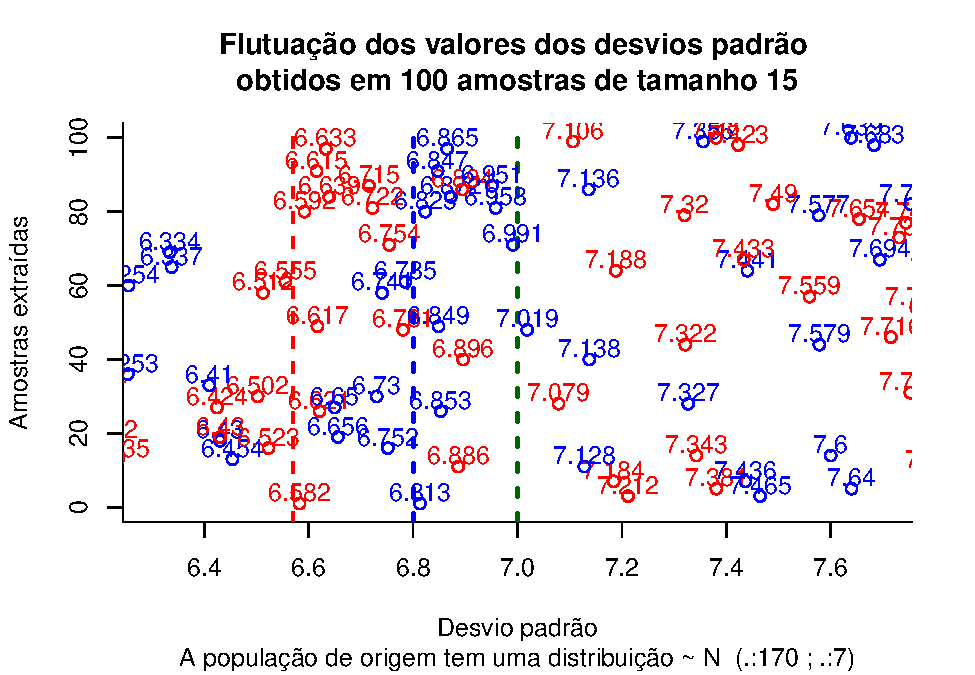
\includegraphics[width=1\linewidth]{apostila_files/figure-latex/unnamed-chunk-33-1} 

}

\caption{Flutuação dos valores do desvio padrão obtidos pelo estimador não viesado (em azul) e pelo estimador viesado (em vermelho) para diversas amostras extraídas de uma mesma população distribuição $\sim N (\mu; \sigma)$ (em verde o desvio padrão populacional, em azul a média dos desvios padrão amostrais correta e em vermelho a estimada de modo viesado)}\label{fig:unnamed-chunk-33}
\end{figure}

\hfill\break

\begin{figure}

{\centering 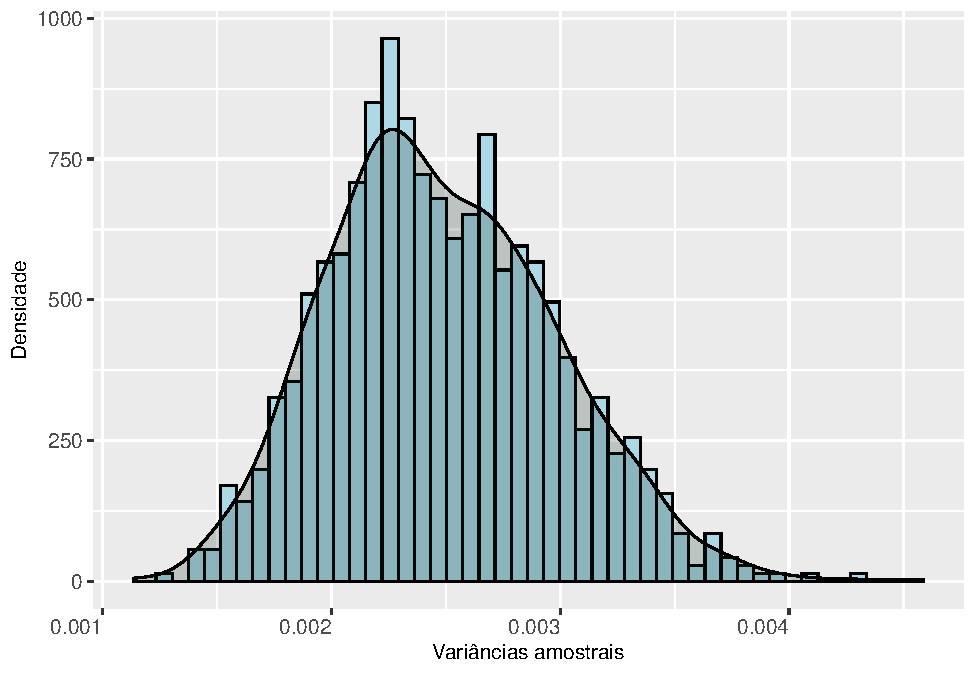
\includegraphics[width=0.8\linewidth]{apostila_files/figure-latex/unnamed-chunk-34-1} 

}

\caption{A distribuição das variâncias amostrais segue uma curva aproximada pela distribuição Qui-quadrado com (n-1) graus de liberdade}\label{fig:unnamed-chunk-34}
\end{figure}

\hfill\break

Uma medida de dispersão que apresenta a mesma unidade que a das observações originais é o \textbf{desvio-padrão}, definido como a raiz quadrada positiva da variância.

\hfill\break

\[
S= \sqrt{\frac{\sum _{i=1}^{n}\left(x_{i}-\stackrel{-}{x}\right)^{2}}{n-1}}
\]

\hfill\break

Tanto a variância quanto o desvio padrão indicam, em média, qual será o erro (desvio) cometido ao tentar substituir cada observação pela medida resumo do conjunto de dados (média).

\hfill\break

Usando os dados das medidas das alturas dos 60 estudantes teremos o seguinte valor para a \textbf{variância} (com unidade igual a \(m^{2}\)) e o \textbf{desvio padrão} (com unidade igual a \(m\)):

\hfill\break

\begin{Shaded}
\begin{Highlighting}[]
\CommentTok{\# Variãncia}
\FunctionTok{var}\NormalTok{(alturas)}
\end{Highlighting}
\end{Shaded}

\begin{verbatim}
## [1] 0.0130809
\end{verbatim}

\begin{Shaded}
\begin{Highlighting}[]
\CommentTok{\# Desvio padrão}
\FunctionTok{sd}\NormalTok{(alturas) }
\end{Highlighting}
\end{Shaded}

\begin{verbatim}
## [1] 0.1143718
\end{verbatim}

Propriedades da variância:

\hfill\break

\begin{itemize}
\tightlist
\item
  somando-se (ou subtraindo-se) cada um dos elementos do conjunto de dados por uma constante arbitrária, a variância (e o desvio padrão) não se altera; e,
\item
  multiplicando-se (ou dividindo-se) cada um dos elementos do conjunto de dados por uma constante arbitrária, a variância ficará multiplicada (ou dividida) pelo quadrado dessa constante. O desvio padrão fica multiplicado (ou dividido) por essa constante
\end{itemize}

\hfill\break

\begin{Shaded}
\begin{Highlighting}[]
\CommentTok{\# Adicionando{-}se uma constante k=0.05}
\NormalTok{alturas\_ad}\OtherTok{=}\NormalTok{alturas}\FloatTok{+0.05}

\CommentTok{\# Variância não se altera}
\NormalTok{var\_ad}\OtherTok{=} \FunctionTok{var}\NormalTok{(alturas\_ad)}
\NormalTok{var\_ad}
\end{Highlighting}
\end{Shaded}

\begin{verbatim}
## [1] 0.0130809
\end{verbatim}

\begin{Shaded}
\begin{Highlighting}[]
\CommentTok{\# Multiplicando{-}se uma constante k=1.2}
\NormalTok{alturas\_mult}\OtherTok{=}\NormalTok{alturas}\SpecialCharTok{*}\FloatTok{1.2}

\CommentTok{\# Variância fica multiplicada (dividida) pelo quadrado dessa constante)}
\FunctionTok{var}\NormalTok{(alturas\_mult)}
\end{Highlighting}
\end{Shaded}

\begin{verbatim}
## [1] 0.0188365
\end{verbatim}

\begin{Shaded}
\begin{Highlighting}[]
\FunctionTok{all.equal}\NormalTok{(}\FunctionTok{var}\NormalTok{(alturas\_mult), }\FunctionTok{var}\NormalTok{(alturas)}\SpecialCharTok{*}\NormalTok{(}\FloatTok{1.2}\SpecialCharTok{\^{}}\DecValTok{2}\NormalTok{)) }
\end{Highlighting}
\end{Shaded}

\begin{verbatim}
## [1] TRUE
\end{verbatim}

\subsubsection{Coeficiente de variação.}\label{coeficiente-de-variauxe7uxe3o.}

\hfill\break

O coeficiente de variação (uma medida adimensional) é dado pela razão do desvio padrão pela média:

\hfill\break

\[
CV(\%)= 100\cdot(\frac{s}{\stackrel{-}{x}})
\]

\hfill\break

\begin{table}[h]
\centering
\caption{Classificação da variabilidade a partir da medida do Coeficiente de variação}
\begin{tabular}{|c|c|}
\hline 
Classificação  & Medida do Coeficiente de variação (CV \%) \\ 
\hline 
Baixo & $CV \le 10\%$ \\
\hline 
Médio  & $10\% \le CV \le 20\%$ \\
\hline 
Alto  & $20\% \le CV \le 30\%$ \\
\hline 
Muito alto & $CV \ge 30\%$ \\
\hline 
\end{tabular}
\end{table}

\hfill\break

\subsection{Medidas de subdivisão (separatrizes)}\label{medidas-de-subdivisuxe3o-separatrizes}

\hfill\break

Separatrizes (quantis) são \textbf{medidas quantitativas} que delimitam uma \emph{proporção de observações existentes} em um conjunto de dados previamente ordenados \textbf{com valores menores que ela}.

\hfill\break

Assim, se tomamrmos como exemplo a mediana, ela é dita uma separatriz (ou quantil) de 50\% pois \textbf{aproximadamente} 50\% dos dados de um conjunto possuem \textbf{valores menores que ela}.

\hfill\break

Para se \textbf{determinar} qualquer separatriz necessitamos saber antes qual a \textbf{posição} que ela ocupa nos \textbf{dados ordenados crescentemente}: \(x_{1}<x_{2}< \dots< x_{n}\):

\hfill\break

\begin{figure}

{\centering 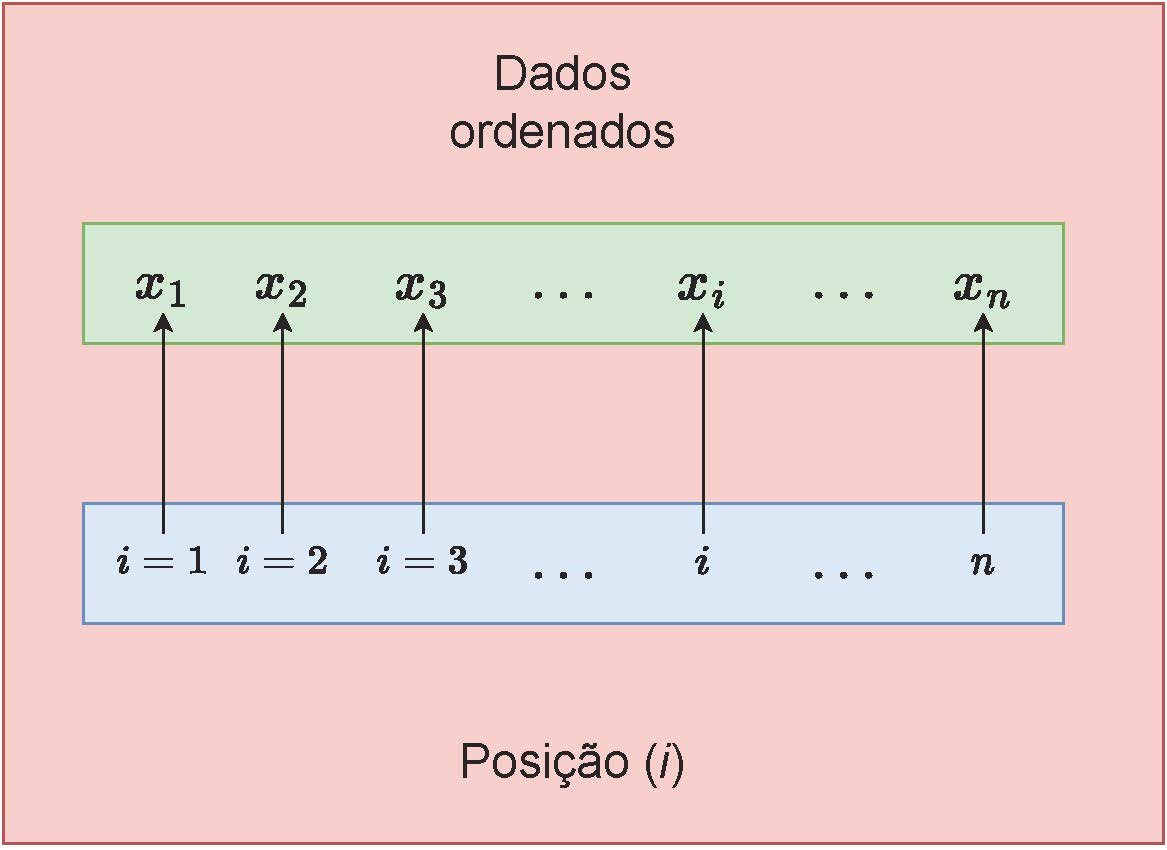
\includegraphics[width=0.5\linewidth]{images3/vetor_posicao} 

}

\caption{Entendendo a indexação de dados}\label{fig:unnamed-chunk-38}
\end{figure}

\hfill\break

De modo geral, um \emph{quantil} de ordem \(p\) (ou também \(p-quantil\), indicado por \(q_{p}\)) é uma medida separatriz onde \(p\) é uma proporção qualquer (limitada no intervalo 0 \textless{} p \textless{} 1), tal que 100\(p\)\% das observações sejam menores que seu valor \(q_{p}\). Desse modo, o valor \(q_{p}\) de uma variável aleatória \(X\) remete à medida da probabilidade:

\hfill\break

\[
P(X=x | x\leq q_{p})=p
\]\\

Os quantis recebem diferentes nomes em função do modo como subdividem o conjunto de dados:

\hfill\break

\begin{itemize}
\tightlist
\item
  percentil (subdivisão em 100 partes): \(p_{1}, \dots, p_{99}\)\\
\item
  decis (subdivisão em 10 partes): \(d_{10}, \dots, d_{90}\)
\item
  quartis (subdivisão em 4 partes): \(Q_{1}, \dots, Q_{3}\)
\end{itemize}

\hfill\break

Naturalmente que os valores de \(p_{50}\), \(d_{5}\) e \(Q_{2}\) são \textbf{os mesmos} posto tratarem-se de separatrizes que subdividem os dados na mesma propoção (50\%).

\hfill\break

Os quantis mais informativos (e que por essa razão são usados para um importante gráfico que mais adiante será exposto em detalhes - \emph{Boxplot}) são: \textbackslash{}

\hfill\break

\begin{itemize}
\tightlist
\item
  1\(^{o}\) Quartil (\(q_{0,25}\)): 25\% dos dados possuem valores abaixo desse valor e 75\% estão acima;
\item
  2\(^{o}\) Quartil ou mediana (\(q_{0,50}\)): 50\% dos dados possuem valores abaixo desse valor e 50\% estão acima; e,
\item
  3\(^{o}\) Quartil (\(q_{0,75}\)): 75\% dos dados possuem valores abaixo desse valor e 25\% estão acima.
\end{itemize}

\hfill\break

Todavia a medicina utiliza para muitos propósitos os percentis como, por exemplo, as curvas de crescimento idade \(versus\) altura.

\hfill\break

De modo geral, para se calcular a posição \emph{L} que um quantil qualquer de ordem \emph{p} assume em um rol de dados há algumas regras empíricas:

\[
L_{p}=\frac{p}{100} \times (n)\\
L_{p}=\frac{p}{100} \times (n+1)\\
L_{p}=[\frac{p}{100} \times (n-1)]+1\\
\]\\

Onde:

\hfill\break

\begin{itemize}
\tightlist
\item
  \emph{p} é a \textbf{ordem} do quantil em \% (50\% no caso mediana, por exemplo);
\item
  \emph{n} é o número de dados do rol; e,
\item
  \emph{L} é a \textbf{posição} do valor referente ao quantil desejado.
\end{itemize}

\hfill\break

Os quartis calculados a partir das posições determinadas por essas regras \emph{aproximadamente} subdividem o conjunto de dados em 25\%, 50\% e 75\%.

\hfill\break

Assim, para a determinação dos quartis pela primeira regra o valor de \emph{p} seria:

\hfill\break

\begin{itemize}
\tightlist
\item
  para o \emph{primeiro quartil} (\(Q_{1}\)): \(L_{q_{0,25}}=\frac{25}{100} \times (n)\);
\item
  para o \emph{segundo quartil} (a mediana ou \(Q_{2}\)): \(L_{q_{0,50}}=\frac{50}{100} \times (n)\); ou,\\
\item
  para o \emph{terceiro quartil} (\(Q_{3}\)): \(L_{q_{0,75}}=\frac{75}{100} \times (n)\).
\end{itemize}

\hfill\break

Novamente podemos nos deparar com \textbf{duas situações possíveis} para o valor calculado para a posição \emph{L} qualquer que seja a regra:

\hfill\break

\begin{itemize}
\tightlist
\item
  se valor calculado da \textbf{posição} L for um \textbf{inteiro}, nessa posição encontraremos o valor referente ao quantil desejado;\\
\item
  se o valor calculado da \textbf{posição L} for \textbf{fracionário}, o valor desse quantil será determinado pela média entre os dois valores dos dados que estão nas \textbf{posições} imediatamente anterior e imediatamente posterior à posição \textbf{L} calculada.
\end{itemize}

\hfill\break

Juntamente com as observações mínima (\(x_{i}\)) e máxima (\(x_{n}\)), o 1\(^{o}\), 2\(^{o}\) e 3\(^{o}\) Quartis são importantes para se ter uma boa idéia da assimetria da distribuição dos dados.

\hfill\break

Para uma distribuição simétrica (ou aproximadamente simétrica) deveremos observar (Distribuição Gaussiana):

\hfill\break

\begin{itemize}
\tightlist
\item
  a dispersão inferior: \(q_{2} - x_{1} \approx x_{n} - q_{2}\) à dispersão superior ;
\item
  \(q_{2} - q_{1}  \approx   q_{3} - q_{2}\); e,
\item
  \(q_{1} - x_{1}  \approx   x_{n} - q_{3}\).
\end{itemize}

\hfill\break

Para nosso conjunto de dados, segundo a regra empírica apresentada teremos as seguintes posições para determinação dos valores dos quartis:

\hfill\break

\begin{itemize}
\tightlist
\item
  para o \emph{primeiro quartil}:
\end{itemize}

\begin{align*}
L_{Q_{1}} & =\frac{p}{100} \times (n) \\
          & =\frac{25}{100} \times (60) \\
          & = 0,25*60 \\
          & = 15
\end{align*}\\

\begin{itemize}
\tightlist
\item
  para o \emph{segundo quartil}:
\end{itemize}

\begin{align*}
L_{Q_{2}} & =\frac{p}{100} \times (n) \\
          & =\frac{50}{100} \times (60) \\
          & = 0,5*60 \\
          & = 30
\end{align*}

\hfill\break
- para o \emph{terceiro quartil}:

\begin{align*}
L_{Q_{3}} & =\frac{p}{100} \times (n) \\
          & =\frac{75}{100} \times (60) \\
          & = 0,75*60 \\
          & = 45
\end{align*}

\hfill\break

E os quartis serão:

\hfill\break

-\(Q_{1}\)=1,63\\
-\(Q_{2}\)=1,67\\
-\(Q_{3}\)=1,75

\hfill\break

Há muitos modos de se estabelecer os quantis descritos na literatura. O próprio \href{https://www.rdocumentation.org/packages/stats/versions/3.6.2/topics/quantile}{R} apresenta 9 modos diferentes:

\hfill\break

\begin{Shaded}
\begin{Highlighting}[]
\FunctionTok{quantile}\NormalTok{(alturas, }\AttributeTok{type=}\DecValTok{1}\NormalTok{)}
\end{Highlighting}
\end{Shaded}

\begin{verbatim}
##   0%  25%  50%  75% 100% 
## 1.41 1.63 1.67 1.75 2.00
\end{verbatim}

\begin{Shaded}
\begin{Highlighting}[]
\FunctionTok{quantile}\NormalTok{(alturas, }\AttributeTok{type=}\DecValTok{2}\NormalTok{)}
\end{Highlighting}
\end{Shaded}

\begin{verbatim}
##    0%   25%   50%   75%  100% 
## 1.410 1.635 1.675 1.755 2.000
\end{verbatim}

\begin{Shaded}
\begin{Highlighting}[]
\FunctionTok{quantile}\NormalTok{(alturas, }\AttributeTok{type=}\DecValTok{3}\NormalTok{)}
\end{Highlighting}
\end{Shaded}

\begin{verbatim}
##   0%  25%  50%  75% 100% 
## 1.41 1.63 1.67 1.75 2.00
\end{verbatim}

\begin{Shaded}
\begin{Highlighting}[]
\FunctionTok{quantile}\NormalTok{(alturas, }\AttributeTok{type=}\DecValTok{4}\NormalTok{)}
\end{Highlighting}
\end{Shaded}

\begin{verbatim}
##   0%  25%  50%  75% 100% 
## 1.41 1.63 1.67 1.75 2.00
\end{verbatim}

\begin{Shaded}
\begin{Highlighting}[]
\FunctionTok{quantile}\NormalTok{(alturas, }\AttributeTok{type=}\DecValTok{5}\NormalTok{)}
\end{Highlighting}
\end{Shaded}

\begin{verbatim}
##    0%   25%   50%   75%  100% 
## 1.410 1.635 1.675 1.755 2.000
\end{verbatim}

\begin{Shaded}
\begin{Highlighting}[]
\FunctionTok{quantile}\NormalTok{(alturas, }\AttributeTok{type=}\DecValTok{6}\NormalTok{)}
\end{Highlighting}
\end{Shaded}

\begin{verbatim}
##     0%    25%    50%    75%   100% 
## 1.4100 1.6325 1.6750 1.7575 2.0000
\end{verbatim}

\begin{Shaded}
\begin{Highlighting}[]
\FunctionTok{quantile}\NormalTok{(alturas, }\AttributeTok{type=}\DecValTok{7}\NormalTok{)}
\end{Highlighting}
\end{Shaded}

\begin{verbatim}
##     0%    25%    50%    75%   100% 
## 1.4100 1.6375 1.6750 1.7525 2.0000
\end{verbatim}

\begin{Shaded}
\begin{Highlighting}[]
\FunctionTok{quantile}\NormalTok{(alturas, }\AttributeTok{type=}\DecValTok{8}\NormalTok{)}
\end{Highlighting}
\end{Shaded}

\begin{verbatim}
##       0%      25%      50%      75%     100% 
## 1.410000 1.634167 1.675000 1.755833 2.000000
\end{verbatim}

\begin{Shaded}
\begin{Highlighting}[]
\FunctionTok{quantile}\NormalTok{(alturas, }\AttributeTok{type=}\DecValTok{9}\NormalTok{)}
\end{Highlighting}
\end{Shaded}

\begin{verbatim}
##       0%      25%      50%      75%     100% 
## 1.410000 1.634375 1.675000 1.755625 2.000000
\end{verbatim}

\hfill\break

Para grandes conjuntos de dados a diferença entre os quantis determinados sob esses diferentes modos será desprezível.

\hfill\break
\#\# Padronização (\emph{z-scores})

\hfill\break

À conversão do valor assumido por uma variável em unidades de desvio padrão acima (ou abaixo) do valor médio de sua distribuição é dado o nome de \emph{padronização}. Essa métrica permite comparações com outras, procedentes de outros fenômenos.

\hfill\break

Para padronizar (achar o seu \emph{z-score} Z) o valor de uma variável procede-se segundo a fórmula:

\hfill\break

\[
Z=\frac{x_{i} - \stackrel{-}{x}}{s}
\]

\hfill\break
O valor \(Z\) expressa quantos desvios esse dado está acima (ou abaixo) da média da distribuição.

\hfill\break

Pelo \emph{Teorema de Tchebichev} pode-se estimar a probabilidade mínima dos dados situados a certa distância de \(k\) desvios da média dessa distribuição:

\hfill\break

\[
P(|X-\mu|\ge k\sigma) \leq 1 - \frac{1}{k^{2}}
\]

\hfill\break

Assim, se \(k=2\) \textbf{ao menos} 75\% das observações devem estar entre a média e dois desvios padrões acima ou abaixo da média.

\hfill\break

\begin{Shaded}
\begin{Highlighting}[]
\NormalTok{med}\OtherTok{=}\FunctionTok{round}\NormalTok{(}\FunctionTok{mean}\NormalTok{(alturas),}\DecValTok{2}\NormalTok{)}
\NormalTok{desv}\OtherTok{=} \FunctionTok{round}\NormalTok{(}\FunctionTok{sd}\NormalTok{(alturas),}\DecValTok{2}\NormalTok{)}
\end{Highlighting}
\end{Shaded}

\hfill\break

No exemplo das alturas dos estudantes temos a média de 1.69 m e um desvio padrão de 0.11 m. Assim, \textbf{ao menos} 75\% das alturas deverão estar entre 1.47 m e 1.91 m.

\hfill\break

\begin{Shaded}
\begin{Highlighting}[]
\FunctionTok{sort}\NormalTok{(alturas)}
\end{Highlighting}
\end{Shaded}

\begin{verbatim}
##  [1] 1.41 1.44 1.47 1.54 1.55 1.56 1.56 1.56 1.57 1.58 1.58 1.61 1.62 1.62 1.63
## [16] 1.64 1.64 1.65 1.65 1.65 1.65 1.66 1.66 1.66 1.66 1.66 1.67 1.67 1.67 1.67
## [31] 1.68 1.68 1.68 1.69 1.71 1.71 1.72 1.72 1.73 1.73 1.73 1.73 1.73 1.74 1.75
## [46] 1.76 1.76 1.77 1.78 1.78 1.79 1.82 1.83 1.83 1.84 1.85 1.86 1.93 1.95 2.00
\end{verbatim}

\begin{Shaded}
\begin{Highlighting}[]
\CommentTok{\# Duas observações menores que 1,47m e trẽs maiores que 1,91m.}
\CommentTok{\# Assim, 54 observações dentro do intervalo, equivalendo a 91,66\% do total.}
\end{Highlighting}
\end{Shaded}

\hfill\break

\section{Medidas de forma (assimetria \& curtose)}\label{medidas-de-forma-assimetria-curtose}

\hfill\break

Quando analisamos o histograma (a representação gráfica da distribuição das frequências dos valores agrupados em classes) de uma determinada variável, não é muito comum que ele se mostre simétrico tal como seria se os dados fossem distribuídos de modo exatamente Normal.

\hfill\break

Ao observarmos que a cauda se mostra mais alongada para a direita (indicativo da existência de uma quantidade maior de dados com grandes valores, \emph{arrastando} a média para a direita: moda \(<\) mediana \(<\) média) diz-se que a \emph{distribuição é assimétrica à direita}. Na situação oposta (moda \(>\) mediana \(>\) média) diz-se que ela é \emph{assimétrica à esquerda}.

\hfill\break

\begin{Shaded}
\begin{Highlighting}[]
\NormalTok{a}\OtherTok{=}\FunctionTok{rbeta}\NormalTok{(}\DecValTok{10000}\NormalTok{,}\DecValTok{5}\NormalTok{,}\DecValTok{2}\NormalTok{)}
\NormalTok{c}\OtherTok{=}\FunctionTok{rbeta}\NormalTok{(}\DecValTok{10000}\NormalTok{,}\DecValTok{5}\NormalTok{,}\DecValTok{5}\NormalTok{)}
\NormalTok{b}\OtherTok{=}\FunctionTok{rbeta}\NormalTok{(}\DecValTok{10000}\NormalTok{,}\DecValTok{2}\NormalTok{,}\DecValTok{5}\NormalTok{)}

\FunctionTok{par}\NormalTok{(}\AttributeTok{mfrow=}\FunctionTok{c}\NormalTok{(}\DecValTok{1}\NormalTok{,}\DecValTok{3}\NormalTok{))}
\FunctionTok{hist}\NormalTok{(a, }
     \AttributeTok{xlab=}\StringTok{"Valores"}\NormalTok{,}\AttributeTok{col =} \StringTok{\textquotesingle{}lightblue\textquotesingle{}}\NormalTok{,}
     \AttributeTok{ylab=}\StringTok{"Frequência"}\NormalTok{,}
     \AttributeTok{main=}\StringTok{"Assimetria à esq."}\NormalTok{)}
\FunctionTok{hist}\NormalTok{(c, }
     \AttributeTok{xlab=}\StringTok{"Valores"}\NormalTok{,}\AttributeTok{col =} \StringTok{\textquotesingle{}lightblue\textquotesingle{}}\NormalTok{,}
     \AttributeTok{ylab=}\StringTok{"Frequência"}\NormalTok{,}
     \AttributeTok{main=}\StringTok{"Relativa simetria"}\NormalTok{)}
\FunctionTok{hist}\NormalTok{(b, }
     \AttributeTok{xlab=}\StringTok{"Valores"}\NormalTok{,}\AttributeTok{col =} \StringTok{\textquotesingle{}lightblue\textquotesingle{}}\NormalTok{,}
     \AttributeTok{ylab=}\StringTok{"Frequência"}\NormalTok{,}
     \AttributeTok{main=}\StringTok{"Assimetria à dir."}\NormalTok{)}
\end{Highlighting}
\end{Shaded}

\begin{figure}

{\centering 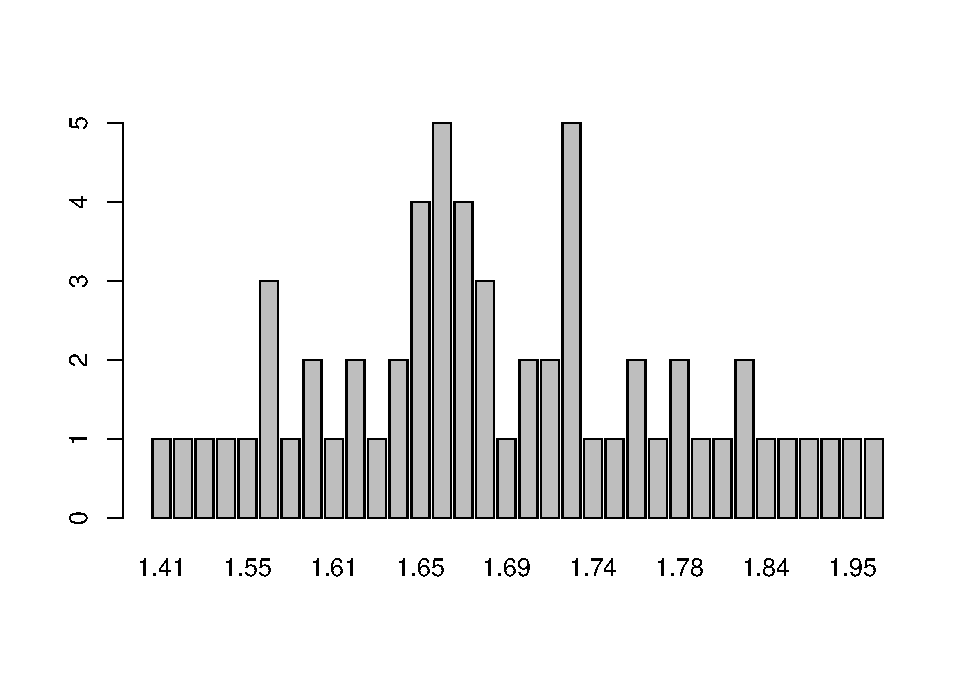
\includegraphics[width=0.8\linewidth]{apostila_files/figure-latex/unnamed-chunk-42-1} 

}

\caption{Diferentes formas na distribuição dos dados}\label{fig:unnamed-chunk-42}
\end{figure}

\hfill\break

De modo assemelhado, o histograma pode denotar uma forma mais \emph{plana} ou menos \emph{aguda}, onde um \emph{cume} mostra-se mais destacado.

\hfill\break

Nesse aspecto da forma, uma variável com distribuição Gaussiana apresentaria uma curva a que denominamos \emph{mesocúrtica}. Distribuições com um aspecto mais plano são denominadas de \emph{platicúrticas} e as com um cume agudo são denominadas \emph{leptocúrticas}.

\hfill\break

A curtose é uma medida da agudeza da distribuição dos dados em relação à distribuição Gaussiana.

\hfill\break

\begin{figure}

{\centering 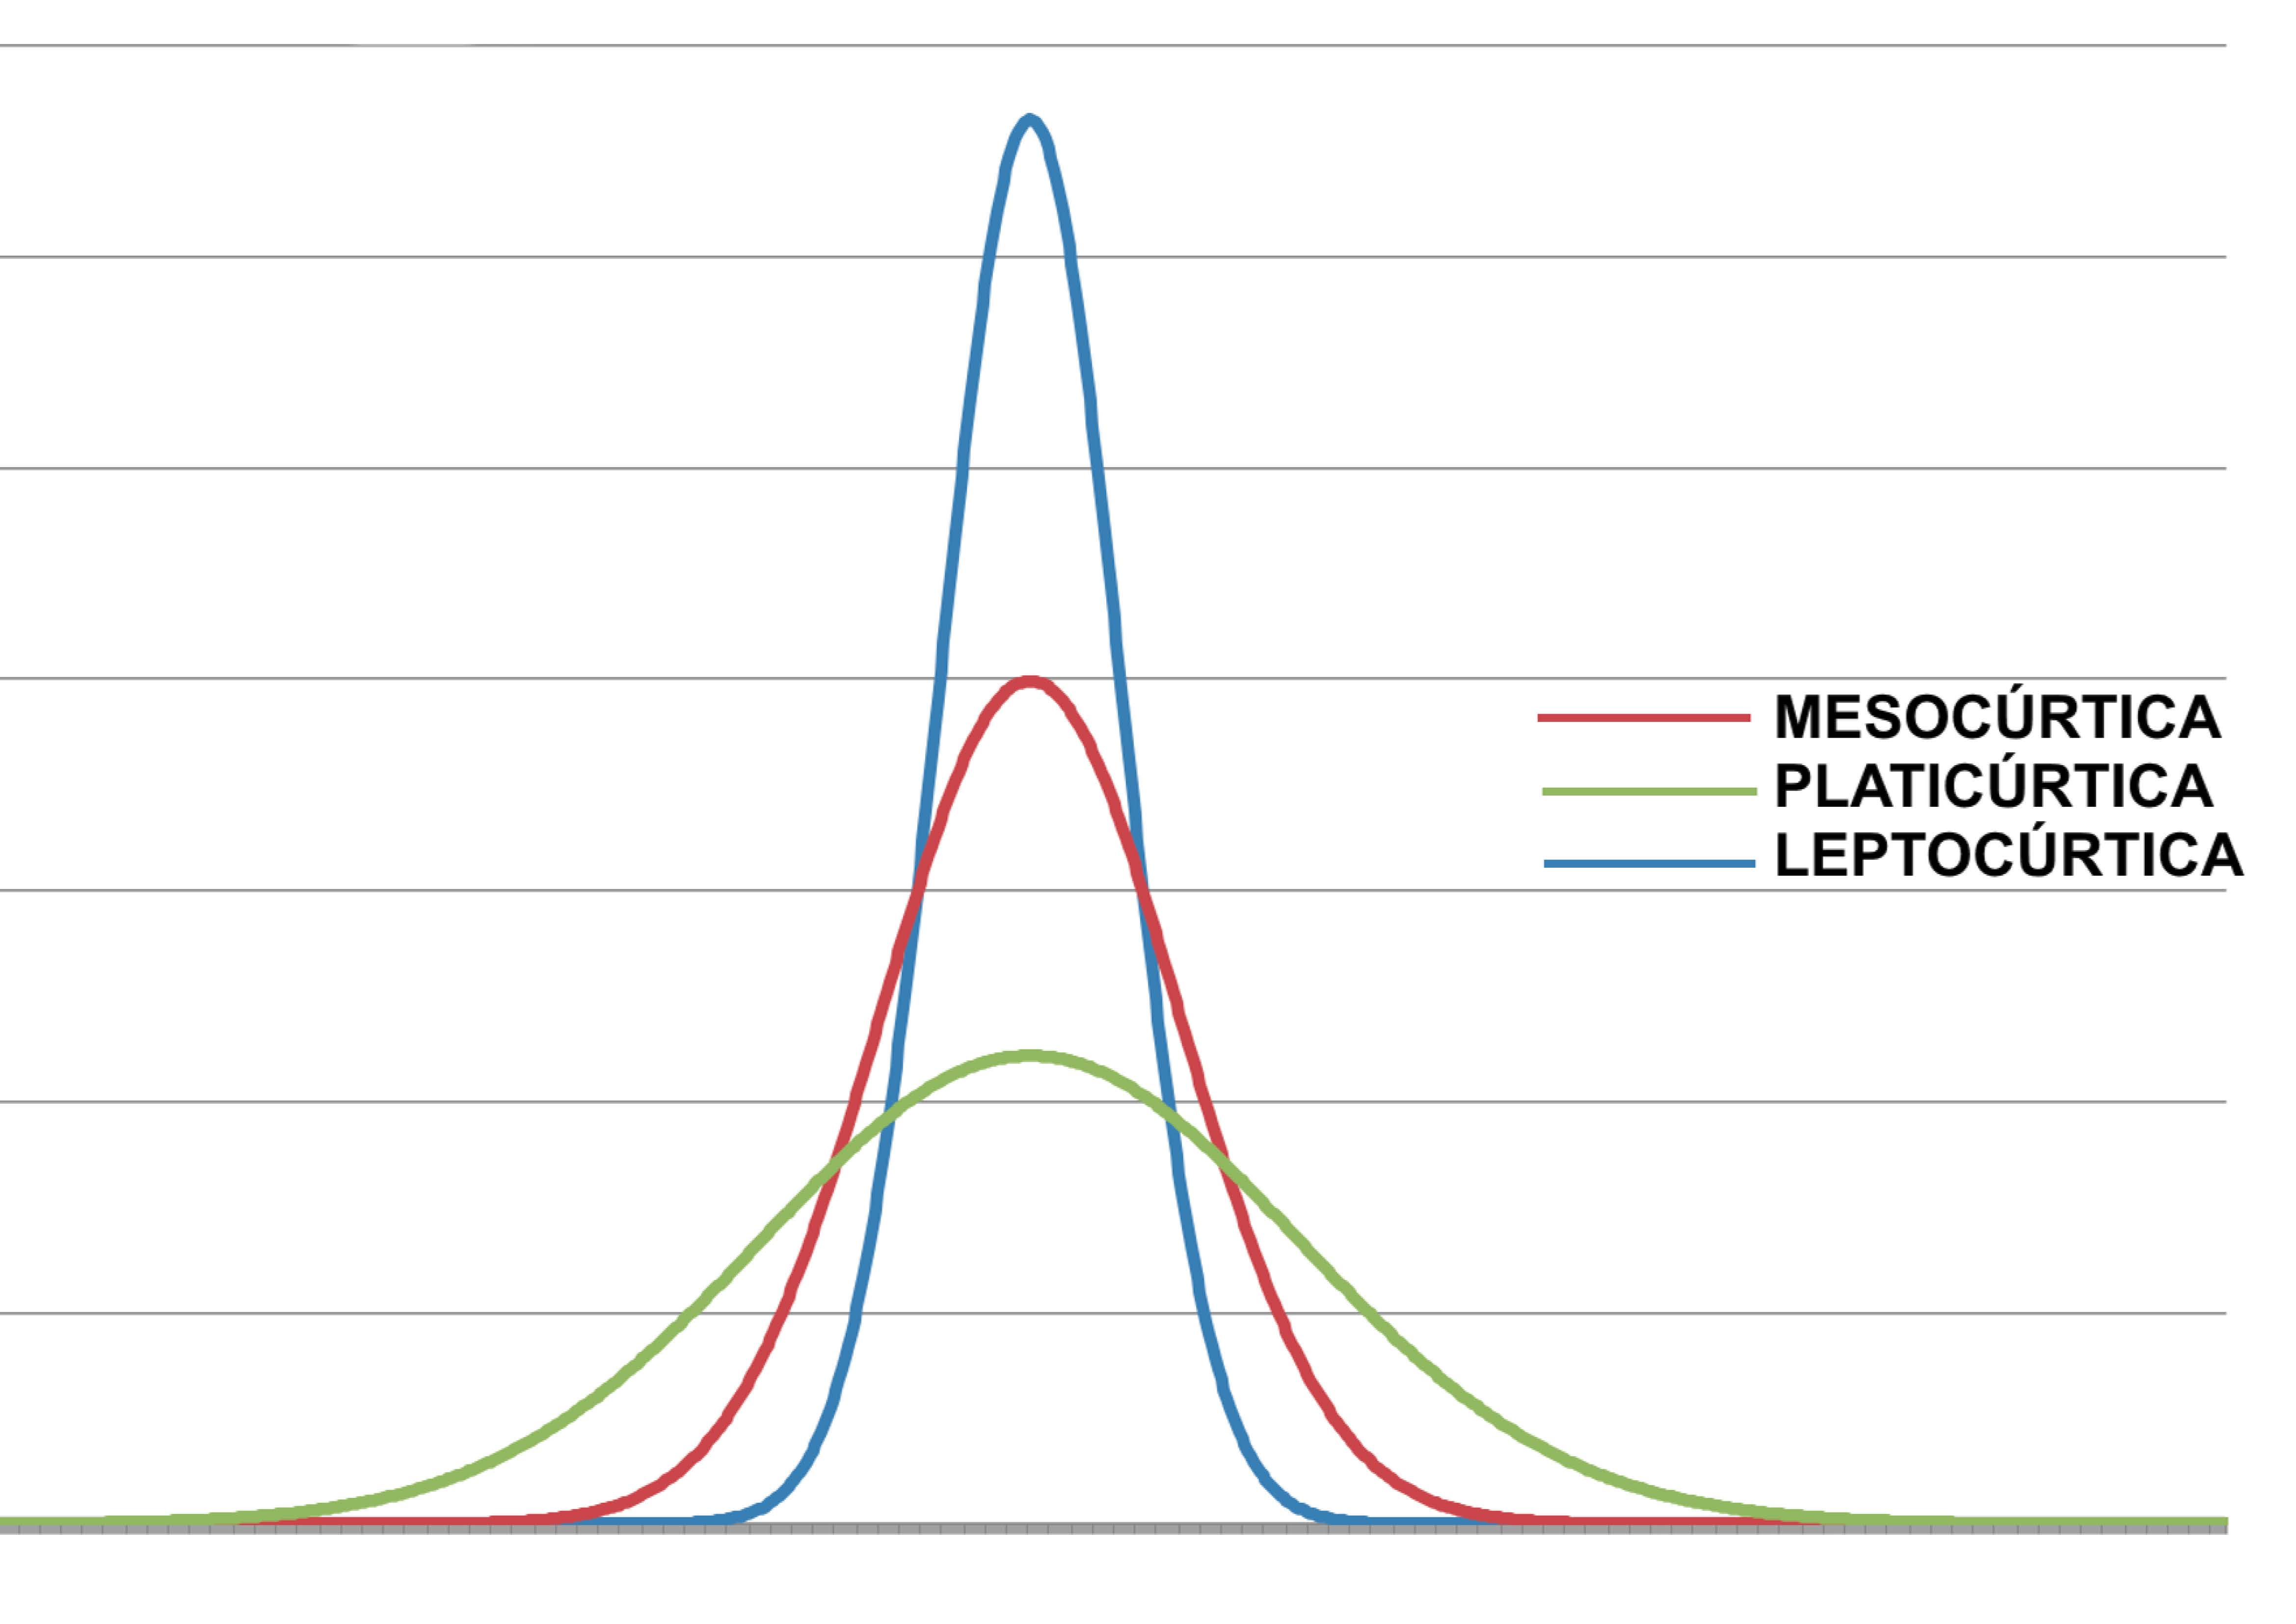
\includegraphics[width=0.8\linewidth]{images3/curtose} 

}

\caption{Diferentes aspectos de uma distribuição quanto à sua inclinação}\label{fig:unnamed-chunk-43}
\end{figure}

\hfill\break

Essas possíveis variações na forma de uma distribuição podem ser numericamente quantificadas através dos \emph{coeficientes de assimetria e curtose}.

\hfill\break

Uma das medidas do coeficiente de assimetria é através do \emph{primeiro ou segundo coeficientes de Pearson}, dados pelas seguintes relações:

\hfill\break

\begin{itemize}
\tightlist
\item
  Primeiro coeficiente de assimetria de Pearson: \(AS= \frac{ \stackrel{-}{x} - M_{o} }{ s }\)
\item
  Segundo coeficiente de assimetria de Pearson: \(AS = \frac{ 3 ( \stackrel{-}{x} - Q_{2}) } { s  }\)
\end{itemize}

\hfill\break

Onde:

\hfill\break

\begin{itemize}
\tightlist
\item
  \(\stackrel{-}{x}\) é a média;
\item
  \(M_{o}\) é a moda;
\item
  \(S\) é o desvio padrão; e,
\item
  \(Q_{2}\) é o segundo quartil (mediana).
\end{itemize}

\hfill\break

A \emph{assimetria} é classificada do modo seguinte:

\hfill\break

\begin{itemize}
\tightlist
\item
  \(-1 \leq AS \leq 1%=
  \) : distribuição simétrica;
\item
  \(AS<-1\): distribuição com assimetria negativa; e,
\item
  \(AS>1\): distribuição com assimetria positiva.
\end{itemize}

\hfill\break

Uma das medidas do coeficiente de curtose é através da seguinte relação entre \emph{quartis} e \emph{percentis}:

\hfill\break

\[
K = \frac{Q_{3} - Q_{1}}   {2 \times(P_{90} - P_{10})} 
\]

\hfill\break

Onde:

\hfill\break

\begin{itemize}
\tightlist
\item
  \(Q_{3}\) = \(3^{o}\) quartil;
\item
  \(Q_{1}\) = \(1^{o}\) quartil;
\item
  \(P_{90}\) = \(90^{o}\) percentil; e,
\item
  \(P_{10}\) = \(10^{o}\) percentil.
\end{itemize}

\hfill\break

O \emph{coeficiente de curtose} é classificado do modo seguinte:

\hfill\break

\begin{itemize}
\tightlist
\item
  k = 0,263: distribuição mesocúrtica;
\item
  k \textless{} 0,263: distribuição leptocúrtica; e,
\item
  k \textgreater{} 0,263: distribuição platicúrtica.
\end{itemize}

\hfill\break

\section{\texorpdfstring{Diferentes posições da média, moda e mediana (2\(^{o}\) quartil)}{Diferentes posições da média, moda e mediana (2\^{}\{o\} quartil)}}\label{diferentes-posiuxe7uxf5es-da-muxe9dia-moda-e-mediana-2o-quartil}

\hfill\break

Essas três medidas podem se apresentar com valores em posições alternadas quando as comparamos:\\

\begin{itemize}
\tightlist
\item
  quando a moda=mediana=média temos uma distribuição de frequências razoavelmente \textbf{simétrica};
\item
  quando a moda \(\leq\) mediana \(\leq\) média (há uma quantidade maior de dados com grandes valores, arrastando a média para a direita, para cima) temos uma distribuição de frequências \textbf{positivamente assimétrica}, ; e,\\
\item
  quando a moda \(\geq\) mediana \(\geq\) média (há uma quantidade maior de dados com pequenos valores, arrastando a média para a esquerda, para baixo) temos uma distribuição de frequências \textbf{negativamente assimétrica}.
\end{itemize}

\hfill\break

\hfill\break

\begin{Shaded}
\begin{Highlighting}[]
\FunctionTok{barplot}\NormalTok{(tab\_alturas,}
        \AttributeTok{main=}\StringTok{"Valores observados da alturas dos estudantes"}\NormalTok{,}
        \AttributeTok{xlab=}\StringTok{"Altura (cm)"}\NormalTok{,}
        \AttributeTok{ylab=}\StringTok{"Quantidade observada (un)"}\NormalTok{,}
        \AttributeTok{ylim=}\FunctionTok{c}\NormalTok{(}\DecValTok{0}\NormalTok{,}\DecValTok{6}\NormalTok{),}
        \AttributeTok{col=}\StringTok{"blue"}\NormalTok{,}
        \AttributeTok{las=}\DecValTok{0}\NormalTok{, }
        \AttributeTok{hor=}\StringTok{"FALSE"}\NormalTok{)}
\FunctionTok{abline}\NormalTok{(}\AttributeTok{v=}\FunctionTok{mean}\NormalTok{(}\FloatTok{19.9}\NormalTok{, }\FloatTok{21.1}\NormalTok{), }\AttributeTok{col=}\StringTok{"red"}\NormalTok{)}
\FunctionTok{text}\NormalTok{( }\FunctionTok{mean}\NormalTok{(}\FloatTok{19.9}\NormalTok{, }\FloatTok{21.1}\NormalTok{)}\SpecialCharTok{{-}}\FloatTok{0.5}\NormalTok{, }\DecValTok{5}\NormalTok{, }\StringTok{"Média=1,69 m"}\NormalTok{, }\AttributeTok{col =} \StringTok{"red"}\NormalTok{, }\AttributeTok{srt=}\DecValTok{90}\NormalTok{)}
\FunctionTok{abline}\NormalTok{(}\AttributeTok{v=}\FunctionTok{median}\NormalTok{(}\FloatTok{18.7}\NormalTok{ , }\FloatTok{19.9}\NormalTok{), }\AttributeTok{col=}\StringTok{"darkgreen"}\NormalTok{) }
\FunctionTok{text}\NormalTok{(}\FunctionTok{median}\NormalTok{(}\FloatTok{18.7}\NormalTok{ , }\FloatTok{19.9}\NormalTok{)}\SpecialCharTok{{-}}\FloatTok{0.5}\NormalTok{, }\DecValTok{5}\NormalTok{, }\StringTok{"Mediana=1,675 m"}\NormalTok{, }\AttributeTok{col =} \StringTok{"darkgreen"}\NormalTok{, }\AttributeTok{srt=}\DecValTok{90}\NormalTok{)}
\FunctionTok{abline}\NormalTok{(}\AttributeTok{v=}\FunctionTok{c}\NormalTok{(}\FloatTok{16.3}\NormalTok{, }\FloatTok{23.5}\NormalTok{), }\AttributeTok{col=}\StringTok{"darkgrey"}\NormalTok{) }
\FunctionTok{text}\NormalTok{(}\FunctionTok{c}\NormalTok{(}\FloatTok{16.3{-}0.5}\NormalTok{, }\FloatTok{23.5{-}0.5}\NormalTok{), }\DecValTok{5}\NormalTok{, }\FunctionTok{c}\NormalTok{(}\StringTok{"Moda=1,66"}\NormalTok{,}\StringTok{"Moda=1,73"}\NormalTok{), }\AttributeTok{col =} \StringTok{"darkgray"}\NormalTok{, }\AttributeTok{srt=}\DecValTok{90}\NormalTok{)}
\end{Highlighting}
\end{Shaded}

\begin{figure}

{\centering \includegraphics[width=0.8\linewidth]{apostila_files/figure-latex/unnamed-chunk-45-1} 

}

\caption{Valores observados das alturas dos estudantes e as posições da média, moda e mediana}\label{fig:unnamed-chunk-45}
\end{figure}

\hfill\break

\begin{figure}

{\centering \includegraphics[width=0.8\linewidth]{images3/comp_sinteses} 

}

\caption{Quadro comparativo entre as medidas de tendência central (posição)}\label{fig:unnamed-chunk-46}
\end{figure}

\section{Apresentação tabular de dados}\label{apresentauxe7uxe3o-tabular-de-dados}

\hfill\break

As sínteses numéricas expostas condensam ao máximo a informação trazida pelos dados na forma de estatísticas associadas à:

\hfill\break

\begin{itemize}
\tightlist
\item
  posição: média, moda, mediana;
\item
  dispersão: amplitude total dos dados, variância (esvio padrão), coeficiente de variação;
\item
  separatrizes (repartição): como por exemplo os quartis (\(Q_{1}\); \(Q_{2}\)/mediana e \(Q_{3}\)).
\end{itemize}

\hfill\break

A correta exposição dos dados na forma de tabelas e gráficos auxilia o entendimento de muitas outras características relacionadas aos dados trabalhados por parte do leitor com grande riqueza visual.

\hfill\break

Ao se lidar com grandes conjuntos de dados a visualização da informação contida nos dados fica comprometida se eles forem simplesmente apresentados como uma listagem, mesmo que depurados de eventuais inconsistências e ordenados como a lista abaixo:

\hfill\break

\begin{Shaded}
\begin{Highlighting}[]
\FunctionTok{sort}\NormalTok{(alturas)}
\end{Highlighting}
\end{Shaded}

\begin{verbatim}
##  [1] 1.41 1.44 1.47 1.54 1.55 1.56 1.56 1.56 1.57 1.58 1.58 1.61 1.62 1.62 1.63
## [16] 1.64 1.64 1.65 1.65 1.65 1.65 1.66 1.66 1.66 1.66 1.66 1.67 1.67 1.67 1.67
## [31] 1.68 1.68 1.68 1.69 1.71 1.71 1.72 1.72 1.73 1.73 1.73 1.73 1.73 1.74 1.75
## [46] 1.76 1.76 1.77 1.78 1.78 1.79 1.82 1.83 1.83 1.84 1.85 1.86 1.93 1.95 2.00
\end{verbatim}

\hfill\break

Um dos modos de se lidar com isso é condensando a informação dos dados brutos em tabelas.

\hfill\break

Uma tabela é uma forma não discursiva de apresentar informações nas quais o dado numérico se destaca como informação central. Uma tabela se diferencia de um quadro por este ter todos os seus campos delimitados por linhas e conter apenas informações de natureza qualitativa.

\hfill\break

Uma tabela deve conter algumas \textbf{informações essenciais}, fora daquela estritamente relacionada aos dados, para que a compreensão do leitor acerca dos dados expostos seja a mais imediata possível:

\hfill\break

\begin{itemize}
\tightlist
\item
  título que explique o que a tabela contém, local, data;
\item
  cabeçalho nas colunas e linhas com a explicação, ainda que resumis, a que se referem as quantidades expostas no corpo;
\item
  corpo formado pelos dados referentes às variáveis;
\item
  fonte dos dados;
\item
  uniformidade no número de casas decimais apresentadas no corpo;
\item
  todas as casas devem apresentar valores ou símbolos que expliquem a ausência da informação (NI, NE, ou 0-zero).
\end{itemize}

\hfill\break

Trabalhos de natureza acadêmica ou científica deveriam obrigatoriamente seguir, quando publicados no Brasil, a norma vigente publicada pela ABNT: Associação Brasileira de Normas Técnicas e algumas punlicações do IBGE: Instituto Brasileiro de Geografia e Estatística (como em \href{https://biblioteca.ibge.gov.br/visualizacao/livros/liv23907.pdf}{link}).

\hfill\break

Observa-se frequentemente, todavia, que as publicações seguem normas particulares das instituições de ensino (para trabalhos de conclusão de curso, monografias, dissertações e teses) ou das editoras (artigos), muitas vezes mescladas com recomendações da ABNT. Na Universidade Estadual de Londrina o portal da biblioteca possui uma ligação para a seção ``Normas para trabalhos'' (\href{https://sites.uel.br/bibliotecas/}{link}).

\hfill\break

\subsection{Apresentação tabular de dados qualitativos}\label{apresentauxe7uxe3o-tabular-de-dados-qualitativos}

\hfill\break

\subsubsection{Dados qualitativos em entrada única}\label{dados-qualitativos-em-entrada-uxfanica}

\hfill\break

Para alguns tipos de dados, a apresentação tabular é bastante imediata.

\hfill\break

Admita que tenha sido realizada uma pesquisa junto a um terminal de desembarque internacional em algum aeroporto sobre o continente de procedência do passageiro, num determinado período de um certo dia, tendo sido anotados os seguintes valores: AM, AM, A, A, A, AM, EU, EU, EU, EU, AM, AS, AS, AS, OC, AS, EU, AM, onde os continente anotados são assim identificados: americano (AM); africano (A), europeu (EU); asiático (AS) e da oceania (OC). Uma tabela para a apresentação dos resultados poderia ser:

\hfill\break

\begin{table}[h]
\begin{center}
\caption{Desembarques no terminal internacional A em Cumbica (SP, Brasil-10/10/2021: 8 h 00min às 12 h 00 min)}
\begin{tabular}{|l|l|}
\hline
Continente de procedência   &  Desembarques  \\
\hline
América & 5 \\                                
África  & 3 \\                           
Europa  & 5 \\                          
Ásia    & 4 \\                          
Oceania & 1 \\                        
\hline
Total  & 18 \\   
\hline
\end{tabular} \vspace{4pt}

Fonte: Próprio autor
\end{center}
\end{table}


\hfill\break

Outro exemplo de apresentação tabular onde são apresentadas as proporções relativas observadas de cada nível da variável estudada (``tipo de família'', com quatro níveis diferentes), de um levantamento amostral feito pela Agência do Censo dos Estados Unidos em 2005.

\hfill\break

\begin{table}[h]
\begin{center}
\caption{Estrutura domiciliar dos Estados Unidos}
\begin{tabular}{|l|l|l|l|}
\hline
Estrutura domiciliar   & Número (milhões)  & Freq. rel.  & Freq. rel.  (\%) \\
\hline
Casal com filhos       & 24,1             & 0,22       & 22               \\
Casal sem filhos       & 31,1             & 0,28       & 28               \\
Solteiro, sem parceiro & 19,1             & 0,17       & 17               \\
Morando sozinho        & 30,1             & 0,27       & 27               \\
Outros domicílios      & 6,7              & 0,06       & 6                \\
\hline
Total                  & 111.1            & 1,00       & 100\%            \\
\hline
\end{tabular} \vspace{4pt}

Fonte: Próprio autor
\end{center}
\end{table}

\hfill\break

\subsubsection{Dados qualitativos em entrada dupla}\label{dados-qualitativos-em-entrada-dupla}

\hfill\break

Outros tipos de dados são provenientes de pesquisas que têm por base respostas de natureza binária como, por exemplo:

\hfill\break

\begin{itemize}
\tightlist
\item
  sim ou não;
\item
  gosto ou não gosto;
\item
  voto em ``A'' ou voto em ``B''; ou,
\item
  concordo ou não concordo.
\end{itemize}

\hfill\break

Como resultado final, são obtidas contagens que expressam as frequências absolutas observadas para cada uma das variáveis (ou seus níveis) como na apresentação tabular de dados qualitativos por \emph{Tabelas de Contingência}.

\hfill\break

As \emph{tabelas de contingência} são usadas para associar duas ou mais variáveis qualitativas (ou seus níveis) às contagens das respostas obtidas, na forma das frequências absoluta e relativa observadas em cada uma dessas variáveis (ou seus níveis).

\hfill\break

O uso desse tipo de tabela é comum quando se pretende investigar se as variáveis estudadas têm alguma associação por meio de testes não paramétricos. Esse tipo de apresentação facilita a extração de informações relacionadas às probabilidades marginais ou condicionadas de cada uma variáveis ou seus níveis.

\hfill\break

Admita agora que a pesquisa anterior junto ao terminal de desembarque internacional tenha também apontado o sexo do passageiro em seu desembarque. Uma tabela de dupla entrada com aqueles dados assumiria a forma:

\hfill\break

\begin{table}
\begin{center}
\caption{Desembarques no terminal internacional A em Cumbica (SP, Brasil - 10/10/2021: 8 h 00min às 12 h 00 min)}
\begin{tabular}{l|l|l|l}
\hline
\multirow{2}{*}{Desembarques no terminal internacional A em Cumbica (SP, Brasil)} & \multicolumn{2}{c|}{Sexo do passageiro} & \multirow{2}{*}{Total}  \\ 
\cline{2-3}
                & M & F &        \\ 
\hline
América & 3 & 2 & 5 \\                                
África  & 3 & 0 & 3 \\                           
Europa  & 1 & 4 & 5 \\                          
Ásia    & 2 & 2 & 4 \\                          
Oceania & 0 & 1 & 1 \\                        
\hline
Total  & 9 & 9 & 18 \\   
\hline
\end{tabular} \vspace{4pt}

Fonte: Próprio autor
\end{center}
\end{table}

\hfill\break

\hfill\break

Um outro exemplo, usando dados da incidência de baixo peso ao nascer em recém-nascidos de Pelotas (RS) segundo o hábito tabágico da mãe durante a gravidez (1982):

\hfill\break

\begin{table}
\begin{center}
\caption{Incidência de baixo peso ao nascer em recém-nascidos de Pelotas, RS, segundo o hábito tabágico da mãe durante a gravidez (1982)}
\begin{tabular}{c|c|c|c}
\hline
\multirow{2}{*}{Classificação da mãe} & \multicolumn{2}{c|}{Baixo peso ao nascer} & \multirow{2}{*}{Total}  \\ 
\cline{2-3}
                               & Sim & Não &        \\ 
\hline              
Fumante & 275  & 2.144  & 2.419    \\
\hline 
Não fumante & 311  & 4.496  & 4.807   \\
\hline 
Total & 586 & 6.640 & 7.226  \\
\hline
\end{tabular} \vspace{4pt}

Fonte: Próprio autor
\end{center}
\end{table}

\hfill\break

\hfill\break

Ou ainda neste outro estudo que analisa a inclinação partidária de dois tipos de núcleos familiares em relação à presença de filhos:

\hfill\break

\begin{table}[h]
\begin{center}
\caption{Inclinação partidária (frequências absolutas)}
\begin{tabular}{|l|l|l|l|}
\hline
Estrutura domiciliar    & Democrata          & Republicano &  Totais        \\
\hline
Casal com filho(s)    & 762                & 468         & 1230            \\
Casal sem filhos      & 484                & 477         & 961             \\
\hline
Totais                & 1246               & 945         & 2191           \\
\hline
\end{tabular} \vspace{4pt}

Fonte: Próprio autor
\end{center}
\end{table}

\hfill\break

A partir das contagens obtidas na pesquisa (as frequências absolutas), uma tabela com as frequências relativas pode ser construída, passando a apresentar as proporções relativas de cada categoria em relação aos níveis pesquisados:

\hfill\break

\begin{table}[h]
\begin{center}
\caption{Inclinação partidária (frequências relativas)}
\begin{tabular}{|l|l|l|l|}
\hline
Estrutura domiciliar    & Democrata (\%)          & Republicano (\%) &  Totais  (\%)      \\
\hline
Casal com filho(s)    & 34,78                & 21,36         & 56,14            \\
Casal sem filhos      & 22,09                & 21,77         & 43,86             \\
\hline
Totais (\%)           & 56,87               & 43,13         & 100           \\
\hline
\end{tabular} \vspace{4pt}

Fonte: Próprio autor
\end{center}
\end{table}

\subsection{Apresentação tabular de dados quantitativos}\label{apresentauxe7uxe3o-tabular-de-dados-quantitativos}

\hfill\break

Todavia, para grandes quatidades de observações de dados quantitativos, a apresentação na forma de tabelas deve ser precedida do agrupamento dos valores observados em classes. O procedimento estatístico de agrupar os dados em \emph{classes} ou \emph{categorias} envolve construir uma \emph{tabela de distribuição de frequências}.

\hfill\break

Uma \emph{tabela de distribuição de frequências} associa cada \emph{classe} (intervalo) de valores da variável estudada ao número de ocorrências observadas. Como \emph{regra prática}, a repartição dos dados brutos em classes deve sempre observar para que não haja um número excessivo de classes (diminuição da finalidade de resumir os dados, criação de classes sem nenhuma observação) nem tampouco poucas (que não possibilitem a visualização da distribuição e promovam perda da informação original).

\hfill\break

A construção de uma \emph{distribuição de frequências} consiste essencialmente em:

\hfill\break

\begin{itemize}
\tightlist
\item
  escolher as \emph{classes} ou \emph{intervalos} (dados quantitativos) ou \emph{categorias} (dados qualitativos);
\item
  separar ou enquadrar os dados nessas \emph{classes} ou \emph{categorias}; e,
\item
  contar o número de dados de cada \emph{classe} ou \emph{categoria}.
\end{itemize}

\hfill\break

A literatura propõe vários modos para se determinar o número \emph{k} de classes:

\hfill\break

\begin{longtable}[]{@{}
  >{\raggedright\arraybackslash}p{(\columnwidth - 4\tabcolsep) * \real{0.3544}}
  >{\raggedright\arraybackslash}p{(\columnwidth - 4\tabcolsep) * \real{0.3291}}
  >{\raggedright\arraybackslash}p{(\columnwidth - 4\tabcolsep) * \real{0.3165}}@{}}
\toprule\noalign{}
\begin{minipage}[b]{\linewidth}\raggedright
Crítério
\end{minipage} & \begin{minipage}[b]{\linewidth}\raggedright
Tamanho da amostra (\emph{n})
\end{minipage} & \begin{minipage}[b]{\linewidth}\raggedright
Fórmula
\end{minipage} \\
\midrule\noalign{}
\endhead
\bottomrule\noalign{}
\endlastfoot
& n \(\leq\) 25 & k=5 \\
Raiz quadrada & 25 \(\leq\) n \(\leq\) 220 & k=\(\sqrt{n}\) \\
Raiz quadrada & 25 \(\leq\) n \(\leq\) 220 & \(2^{k} > n\) \\
Herbert \textbf{Sturges} & 135 \(\leq\) 572237 & k=1+3,22.log(n)\(^{(1)}\) \\
Giuseppe \textbf{Milone} & 20 \(\leq 36315\) & k=-1+2.ln(n) \(^{(2)}\) \\
\end{longtable}

\hfill\break

\begin{itemize}
\tightlist
\item
  \(^{(1)}\): logarítmo na base 10; e
\item
  \(^{(2)}\): logarítmo na base \emph{e}.
\end{itemize}

\hfill\break

Ao se escolher um número (\(k\)) de classes deve-se \textbf{ponderar} para que:

\hfill\break

\begin{itemize}
\tightlist
\item
  os intervalos das classes tenham, geralmente, a mesma amplitude (raramente se necessita dispor de classes com amplitudes diferentes);
\item
  os intervalos, a faixa de variação que vai do limite inferior da \textbf{primeira classe} ao limite superior da **última classe*, devem conter todos os valores possíveis da variável;
\item
  cada valor observado deve pertencer \textbf{apenas a uma classe};
\item
  nenhuma classe deverá estar vazia (sem observação alguma);\\
\item
  não adotar um número muito elevado de classes de modo que cada classe possua poucas observações (ou mesmo nenhuma); e,
\item
  não adotar um número muito reduzido de classes de modo a esconder a variabilidade dos dados ao se reunir todas as observações em poucas faixas de valores;
\item
  alguns autores recomendam um número mínimo de 5 classes e um máximo de 15;
\item
  podemos considerar a amplitude de cada classe com \textbf{uma casa decimal a mais que os dados} de modo a facilitar a incorporação do último valor (mais elevado) na última classe.
\end{itemize}

\hfill\break

Em nosso exemplo das alturas dos estudantes, a determinação do número de classes pelo critério da \emph{raiz quadrada} ( \emph{n}=60) sugere 8 classes (outros critérios: pelo menor inteiro tq. \(2^{k}>n; k=6\), pelo critério de Sturges \(k=6,86 \sim 7\), de Giuseppe Milone \(k=8,18 \sim 9)\)).

\hfill\break

\begin{align*}
k & =\sqrt{n} \\
 & = 7,74 \\
\end{align*}

\hfill\break

Arredondar para \textbf{mais}: \(k=8\).

\hfill\break

A \emph{amplitude total} (\emph{C}) dos valores observados é a simples diferença entre o \emph{valor máximo} (2,00 m) e o \emph{valor mínimo} (1,41 m):

\hfill\break

\begin{align*}
C & =2,00-1,41 \\
 & =0,59 m 
\end{align*}

\hfill\break

A amplitude de cada uma das classes ( \emph{c}) será dada pelo quociente da \emph{amplitude total} ( \emph{C}) pelo \emph{número de classes} ( \emph{k}).\\

\begin{align*}
c & = \frac{C}{k} \\
  & = \frac{0,59}{8}\\ 
  & = 0,07375 m
\end{align*}

\hfill\break

Arredondar para \textbf{mais}: \(c=0,075 m\).

\hfill\break

As classes são então assim construídas:

\hfill\break

\begin{itemize}
\tightlist
\item
  Limite inferior da \(1^{a}\) classe (\(LI_{1}\)): valor mínimo observado; e,
\item
  Limite superior da \(1^{a}\) classe (\(LS_{1}\)): \(LI_{1}\) + c.~
\end{itemize}

\hfill\break

e assim sucessivamente atá a última classe.

\hfill\break

Símbolos gráficos para intervalos:

\hfill\break

\begin{itemize}
\tightlist
\item
  Os símbolos abaixo indicam que o valor situado à sua esquerda \textbf{está incluído} no intervalo e o da direita \textbf{não está}:
\end{itemize}

~

\[
\vdash \\
{\bullet}-{\circ}
\]

\hfill\break

\begin{itemize}
\tightlist
\item
  Os símbolos abaixo indicam que o valor situado à sua esquerda \textbf{não está} incluído no intervalo e o da direita **está incluído*:
\end{itemize}

\hfill\break

\[
\dashv  \\
{\circ}-{\bullet}
\]

\hfill\break

\begin{quote}
As tabelas que serão apresentadas a seguir estão sem os requisitos essenciais expostos anteriormente uma vez que o propósito é explicar a construção e cálculo dos valores de suas células.
\end{quote}

\hfill\break

Com \(c=0,075m\) as 8 classes ficam assim estabelecidas, tendo-se como ponto de partida o valor mínimo observado: 1,41 m - 1,485 m; 1,485 m - 1,56 m; 1,56 m - 1,635 m; 1,635 m - 1,71 m; 1,71 m - 1,785 m; 1,785 m - 1,86 m; 1,86 m - 1,935m; 1,935 - 2,01 m.

\hfill\break

\{\textcolor{blue}{ 1,41 ; 1,44 ; 1,47} ; 1,54 ; 1,55 ; \textcolor{blue}{1,56 ; 1,56 ; 1,56; 1,57 ; 1,58 ; 1,58 ; 1,61 ; 1,62 ; 1,62 ; 1,63}; 1,64 ;1,64 ; 1,65 ; 1,65 ; 1,65 ; 1,65 ; 1,66 ; 1,66 ; 1,66 ; 1,66 ; 1,66 ; 1,67 ; 1,67 ; 1,67 ; 1,67 ; 1,68 ; 1,68 ;1,68 ; 1,69 ; \textcolor{blue}{ 1,71 ; 1,71 ; 1,72 ; 1,72 ; 1,73 ; 1,73 ; 1,73 ; 1,73 ; 1,73 ; 1,74 ; 1,75 ; 1,76 ; 1,76 ; 1,77 ;  1,78 ; 1,78}; 1,79 1,82 ; 1,83 ; 1,83 ; 1,84 ; 1,85 ; \textcolor{blue}{ 1,86  ; 1,93}; 1,95 ; 2,00\}

\hfill\break
\hfill\break

A tabela de distribuição de frequências com 8 classes, cada uma com amplitude 0,075 m, assume a forma:

\hfill\break

\begin{longtable}[]{@{}ll@{}}
\toprule\noalign{}
Classe & Frequência absoluta (\(f_{i}\)) \\
\midrule\noalign{}
\endhead
\bottomrule\noalign{}
\endlastfoot
1,41 m \(\vdash\) 1,485 m & 3 \\
1,485 m \(\vdash\) 1,56 m & 2 \\
1,56 m \(\vdash\) 1,635 m & 10 \\
1,635 m \(\vdash\) 1,71 m & 19 \\
1,71 m \(\vdash\) 1,785 m & 16 \\
1,785 m \(\vdash\) 1,86 m & 6 \\
1,86 m \(\vdash\) 1,935 m & 2 \\
1,935m \(\vdash\) 2,01 m & 2 \\
Total & 60 \\
\end{longtable}

\hfill\break

Alternativamente, caso adotássemos como ponto de partida (um pouco abaixo do valor mínimo observado) o valor de 1,40 m e como aplitude de classe 0,08 m, uma tabela alternativa de distribuição de frequẽncias teria como classes : 1,40 m - 1,48 m; 1,48 m - 1,56 m; 1,56 m - 1,64 m; 1,64 m - 1,72 m; 1,72 m - 1,80 m; 1,80 m - 1,88 m; 1,88 m - 2,06 m e, para facilitar a contagem das observações pertencentes a cada uma das classes ordenamos os dados:

\hfill\break

\{
\textcolor{blue}{1,41 ; 1,44 ; 1,47 ;}
1,54 ; 1,55 ;
\textcolor{blue}{1,56 ; 1,56 ; 1,56 ; 1,57 ; 1,58 ; 1,58 ; 1,61 ; 1,62 ; 1,62 ; 1,63 ;}
1,64 ;1,64 ; 1,65 ; 1,65 ; 1,65 ; 1,65 ; 1,66 ; 1,66 ; 1,66 ; 1,66 ; 1,66 ; 1,67 ; 1,67 ; 1,67 ; 1,67 ; 1,68 ; 1,68 ;1,68 ; 1,69 ; 1,71 ; 1,71 ;
\textcolor{blue}{1,72 ; 1,72 ; 1,73 ; 1,73 ; 1,73 ; 1,73 ; 1,73 ; 1,74 ; 1,75 ; 1,76 ; 1,76 ; 1,77 ;  1,78 ; 1,78 ;1,79;} 1,82 ; 1,83 ; 1,83 ; 1,84 ; 1,85 ; 1,86 ;
\textcolor{blue}{1,93 ; 1,95 ; 2,00;} \}

\hfill\break

A tabela de distribuição de frequências com 7 classes, cada uma com amplitude 0,08 m, assume a forma:

\hfill\break

\begin{longtable}[]{@{}ll@{}}
\toprule\noalign{}
Classe & Frequência absoluta (\(f_{i}\)) \\
\midrule\noalign{}
\endhead
\bottomrule\noalign{}
\endlastfoot
1,40 m \(\vdash\) 1,48 m & 3 \\
1,48 m \(\vdash\) 1,56 m & 2 \\
1,56 m \(\vdash\) 1,64 m & 10 \\
1,64 m \(\vdash\) 1,72 m & 21 \\
1,72 m \(\vdash\) 1,80 m & 15 \\
1,80 m \(\vdash\) 1,88 m & 6 \\
1,88 m \(\vdash\) 2,06 m & 3 \\
Total & 60 \\
\end{longtable}

\hfill\break

Também podemos cogitar adotar alternativamente um intervalo de classe \(c=0,10\) m, com a primeira classe começando (um pouco abaixo do valor mínimo observado) na altura de 1,40 m; todavia, a última classe não iria contemplar o valor máximo observado (2,00 m) e necessitaíamos abrir mais uma classe apenas para incluí-lo.

\hfill\break

Mas começando-se no valor mínimo obseravado (1,41 m) estaríamos assegurando que o limite superior da última classe incluiria o valor máximo observado (2,00 m). Assim, essas seriam as classes sob uma amplitude de 0,10 m: 1,41 m - 1,51 m; 1,51 m - 1,61 m; 1,61 m - 1,71 m; 1,71 m - 1,81 m; 1,81 m - 1,91 m; 1,91 m - 2,01 m. O total de 6 classes (1,41 m a 2,01 m) cobre toda faixa de variação dos valores dos dados (de 1,41 m a 2,00 m ) e é de rápida assimilação pelo leitor.

\hfill\break

Ordenando-se os dados para facilitar a contagem das observações pertencentes a cada uma das classes:

\hfill\break

\{\textcolor{blue}{1,41 ; 1,44 ; 1,47 ;} 1,54 ; 1,55 ; 1,56 ; 1,56 ; 1,56 ; 1,57 ; 1,58 ; 1,58 ; \textcolor{blue}{1,61 ; 1,62 ; 1,62 ; 1,63 ; 1,64 ;1,64 ; 1,65 ; 1,65 ; 1,65 ; 1,65 ; 1,66 ; 1,66 ; 1,66 ; 1,66 ; 1,66 ; 1,67 ; 1,67 ; 1,67 ; 1,67 ; 1,68 ; 1,68 ;1,68 ; 1,69 ;} 1,71 ; 1,71 ; 1,72 ; 1,72 ; 1,73 ; 1,73 ; 1,73 ; 1,73 ; 1,73 ; 1,74 ; 1,75 ; 1,76 ; 1,76 ; 1,77 ; 1,78 ; 1,78 ; 1,79 ; \textcolor{blue}{1,82 ; 1,83 ; 1,83 ; 1,84 ; 1,85 ; 1,86 ;} 1,93 ; 1,95 ; 2,00\}

\hfill\break

A tabela de distribuição de frequências com 6 classes, cada uma com amplitude 0,10 m, assume a forma:

\hfill\break

\begin{longtable}[]{@{}ll@{}}
\toprule\noalign{}
Classe & Frequência absoluta (\(f_{i}\)) \\
\midrule\noalign{}
\endhead
\bottomrule\noalign{}
\endlastfoot
1,41 m \(\vdash\) 1,51 m & 3 \\
1,51 m \(\vdash\) 1,61 m & 8 \\
1,61 m \(\vdash\) 1,71 m & 23 \\
1,71 m \(\vdash\) 1,81 m & 17 \\
1,81 m \(\vdash\) 1,91 m & 6 \\
1,91 m \(\vdash\) 2,01 m & 3 \\
Total & 60 \\
\end{longtable}

\hfill\break

\emph{Tabelas de distribuição de frequências} mais completas podem montadas agregando muitas informações adicionais em novas colunas, mediante simples operações aritméticas.

\hfill\break

Essas informações servem para tornar a visualização mais imediata e muitas delas são obtidas com operações matemáticas elementares:

\hfill\break

\begin{itemize}
\tightlist
\item
  Classe \emph{i}: é a simples identificação de cada classe;
\item
  Amplitude (\(\Delta_{i}\)) da classe \(i\): a diferença entre o valor do limite superior e o do inferior de cada classe;
\item
  Intervalo de valores da classe \(i\) (onde seu limite inferior \textbf{está contido} e o limite superior \textbf{não está contido});
\item
  Valor médio (\(\stackrel{-}{x}_{i}\)) de cada classe \(i\): o valor de seu \textbf{limite inferior} mais a metade da amplitude da classe;
\item
  Frequência absoluta (\(f_{i}\)) da classe \(i\): o número de observações contidas no intervalo da classe considerada;
\item
  Frequência relativa (\(fr_{i}= \frac{f_{i}}{n}\)) da classe \(i\) (ou frequência relativa percentual, se assim apresentada): o quociente do número de observações \(n_{i}\) contidas no intervalo da classe \(f_{i}\), pelo número total de observações (\(n\));
\item
  Frequência acumulada (\(fac_{i}\)) da classe \(i\) (ou frequência acumulada percentual, se assim apresentada): o número de observações com medidas contidas na classe \(i\) e nas anteriores a ela;
\item
  Densidade absoluta (\(\delta_{i}=\frac{f_{i}}{\Delta_{i}}\)): o quociente do número de observações da classe (\(f_{i}\)) pela sua amplitude (\(\Delta_{i}\));
\item
  Densidade relativa \(\delta_{fr_{i}}=\frac{fr_{i}}{\Delta_{i}}\): o quociente da frequência relativa (\(fr_{i}\)) pela amplitude (\(\Delta_{i}\)) da classe.
\end{itemize}

\hfill\break

Vejo como exemplo as tabelas abaixo:

\hfill\break

\begin{longtable}[]{@{}
  >{\raggedright\arraybackslash}p{(\columnwidth - 14\tabcolsep) * \real{0.0597}}
  >{\raggedright\arraybackslash}p{(\columnwidth - 14\tabcolsep) * \real{0.1567}}
  >{\raggedright\arraybackslash}p{(\columnwidth - 14\tabcolsep) * \real{0.1866}}
  >{\raggedright\arraybackslash}p{(\columnwidth - 14\tabcolsep) * \real{0.0821}}
  >{\raggedright\arraybackslash}p{(\columnwidth - 14\tabcolsep) * \real{0.1194}}
  >{\raggedright\arraybackslash}p{(\columnwidth - 14\tabcolsep) * \real{0.1343}}
  >{\raggedright\arraybackslash}p{(\columnwidth - 14\tabcolsep) * \real{0.1269}}
  >{\raggedright\arraybackslash}p{(\columnwidth - 14\tabcolsep) * \real{0.1343}}@{}}
\toprule\noalign{}
\begin{minipage}[b]{\linewidth}\raggedright
Classe
\end{minipage} & \begin{minipage}[b]{\linewidth}\raggedright
Int. de valores
\end{minipage} & \begin{minipage}[b]{\linewidth}\raggedright
Alt. média
\end{minipage} & \begin{minipage}[b]{\linewidth}\raggedright
Freq. abs.
\end{minipage} & \begin{minipage}[b]{\linewidth}\raggedright
Freq. rel.
\end{minipage} & \begin{minipage}[b]{\linewidth}\raggedright
Freq. rel. (\%)
\end{minipage} & \begin{minipage}[b]{\linewidth}\raggedright
Freq. acumulada
\end{minipage} & \begin{minipage}[b]{\linewidth}\raggedright
Freq. acum. (\%)
\end{minipage} \\
\midrule\noalign{}
\endhead
\bottomrule\noalign{}
\endlastfoot
& & (\(\stackrel{-}{x}_{i}\)) & (\(f_{i}\)) & (\(fr_{i}\)) & (\(fr_{i}\%\)) & (\(fac_{i}\)) & (\(fac_{i}\%\)) \\
1 & 1,41 \(\vdash\) 1,51 & 1,46 & 3 & 0,05 & 5 & 3 & 5,00 \\
2 & 1,51 \(\vdash\) 1,61 & 1,56 & 8 & 0,13 & 13,33 & 11 & 18,33 \\
3 & 1,61 \(\vdash\) 1,71 & 1,66 & 23 & 0,38 & 38,33 & 34 & 56,66 \\
4 & 1,71 \(\vdash\) 1,81 & 1,76 & 17 & 0,28 & 28,34 & 51 & 85,00 \\
5 & 1,81 \(\vdash\) 1,91 & 1,86 & 6 & 0,10 & 10 & 57 & 95,00 \\
6 & 1,91 \(\vdash\) 2,01 & 1,96 & 3 & 0,05 & 5 & 60 & 100,00 \\
Totais & - & & 60 & 1,00 & 100,00 & - & - \\
\end{longtable}

\hfill\break

\begin{longtable}[]{@{}
  >{\raggedright\arraybackslash}p{(\columnwidth - 12\tabcolsep) * \real{0.0748}}
  >{\raggedright\arraybackslash}p{(\columnwidth - 12\tabcolsep) * \real{0.1963}}
  >{\raggedright\arraybackslash}p{(\columnwidth - 12\tabcolsep) * \real{0.1028}}
  >{\raggedright\arraybackslash}p{(\columnwidth - 12\tabcolsep) * \real{0.1495}}
  >{\raggedright\arraybackslash}p{(\columnwidth - 12\tabcolsep) * \real{0.1495}}
  >{\raggedright\arraybackslash}p{(\columnwidth - 12\tabcolsep) * \real{0.1121}}
  >{\raggedright\arraybackslash}p{(\columnwidth - 12\tabcolsep) * \real{0.2150}}@{}}
\toprule\noalign{}
\begin{minipage}[b]{\linewidth}\raggedright
Classe
\end{minipage} & \begin{minipage}[b]{\linewidth}\raggedright
Int. de valores
\end{minipage} & \begin{minipage}[b]{\linewidth}\raggedright
Freq. abs.
\end{minipage} & \begin{minipage}[b]{\linewidth}\raggedright
Amplitude
\end{minipage} & \begin{minipage}[b]{\linewidth}\raggedright
Dens. abs
\end{minipage} & \begin{minipage}[b]{\linewidth}\raggedright
Freq. rel.
\end{minipage} & \begin{minipage}[b]{\linewidth}\raggedright
Dens. rel.
\end{minipage} \\
\midrule\noalign{}
\endhead
\bottomrule\noalign{}
\endlastfoot
& & (\(f_{i}\)) & (\(\Delta_{i}\)) & (\(\delta_{i}\)) & (\(fr_{i}\)) & (\(\delta_{fr_{i}}\)) \\
1 & 1,41 \(\vdash\) 1,51 & 3 & 0,10 & 30 & 0,05 & 0,5 \\
2 & 1,51 \(\vdash\) 1,61 & 8 & 0,10 & 80 & 0,13 & 1,33 \\
3 & 1,61 \(\vdash\) 1,71 & 23 & 0,10 & 230 & 0,39 & 3,83 \\
4 & 1,71 \(\vdash\) 1,81 & 17 & 0,10 & 170 & 0,28 & 2,83 \\
5 & 1,81 \(\vdash\) 1,91 & 6 & 0,10 & 60 & 0,10 & 1 \\
6 & 1,91 \(\vdash\) 2,01 & 3 & 0,10 & 30 & 0,05 & 0,5 \\
Totais & - & 60 & - & - & 1,00 & - \\
\end{longtable}

\hfill\break

\subsection{Média}\label{muxe9dia-1}

\hfill\break

Nas tabelas de \emph{distribuições de frequências} os resultados estão agrupados em \emph{intervalos de classes (\(i\))}. Por essa razão, os dados perdem sua identidade individual e passam a se representados pelo valor médio de cada intervalo (\(\stackrel{-}{x}_{i}\)).

\hfill\break

A média será então dada pelo produto deste valor médio de cada intervalo (\(\stackrel{-}{x}_{i}\)) pela frequência absoluta que ele apresentou (\({n}_{i}\)), dividido pela quantidade de dados (\(n\)).

\hfill\break

Sejam \(n_{1}, n_{2}, ..., n_{n}\) as frequências apresentadas para cada intervalo \(i\) dos valores assumidos pela variável \(X\) para o total \(n\) de observações. Assim a \emph{média aritmética simples} para dados agrupados será dada por:

\hfill\break

\[
\stackrel{-}{x}=\frac{\sum _{i=1}^{k}{f}_{i}\cdot{\stackrel{-}{x}}_{i}}{n}
\]\\

onde:

\begin{itemize}
\tightlist
\item
  \(\stackrel{-}{x}_{i}\): o valor médio do intervalo da classe \(i\);
\item
  \(f_{i}\): a frequência absoluta da classe \(i\);
\item
  \(k\) é o número de classes da tabela de distribuição de frequências;
\item
  \(n\) é o número de dados da tabela (eventualmente, os dados podem se referir a toda a população sob estudo) .
\end{itemize}

\subsection{Moda}\label{moda-1}

\hfill\break

Moda para dados apresentados na forma de uma distribuição de frequências:

\[
Mo = l_{inf} + (\frac{\Delta_{1}}{\Delta_{1} + \Delta_{2}}) \times \Delta_{i}
\]\\
\strut \\

Primeiramente identificamos a(s) classe(s) modal(is), que é (são) a(s) classe(s) com maior(es) frequência(s) absoluta \(f_{i}\). Os demias elementos da expressã da moda são:\\

\begin{itemize}
\tightlist
\item
  \(l_{inf}\): limite inferior da classe modal;\\
\item
  \(\Delta_{1}\) frequência absoluta da \textbf{classe modal} menos a frequência absoluta da \textbf{classe anterior} à classe modal;
\item
  \(\Delta_{2}\) frequência absoluta da \textbf{classe modal} menos a frequência absoluta da \textbf{classe posterior} à classe modal; e,
\item
  \(\Delta_{i}\) é o intervalo de cada classe.
\end{itemize}

\hfill\break

\subsection{Mediana}\label{mediana}

\hfill\break

Mediana para dados apresentados na forma de uma \textbf{distribuição de frequências}:

\hfill\break

\[
Md = l_{inf} + \left[ \frac{\frac{\sum_{i}^{k} f_{i}}{2} - f_{ac_{(md-1)}}}{f_{md}} \right] \times \Delta_{i}
\]

\hfill\break

Primeiramente identificamos a classe mediana, que é a classe que contem o elemento de posição \(\frac{n}{2}\) (basta observar a coluna da frequência absoluta acumulada: \(f_{ac_i}\), percorrendo-a até a classe \(i\) que tenha valor \(>\frac{n}{2}\). Os demais elementos da expressão da mediana são:

\hfill\break

\begin{itemize}
\tightlist
\item
  \(l_{inf}\): limite inferior da \textbf{classe mediana};\\
\item
  \(f_{ac_{(i-1)}}\): é a frequência absoluta acumulada até a \textbf{classe anterior à classe mediana};\\
\item
  \(f_{md}\): é a frequência absoluta da \textbf{classe mediana}; e,\\
\item
  \(\Delta_{i}\): é o intervalo de cada classe.
\end{itemize}

\hfill\break

\subsection{Variância}\label{variuxe2ncia}

\hfill\break

Variância para dados agrupados:

\hfill\break

\[
S^{2}= \frac{1}{n-1} \times \left[  \sum _{i=1}^{k}{(\stackrel{-}{x}}_{i})^{2} \cdot {f}_{i} - \frac{{\left(\sum _{i=1}^{k}{\stackrel{-}{x}}_{i} \cdot {f}_{i}\right)}^{2}  }{n}\right]
\]

\hfill\break

em que:

\begin{itemize}
\tightlist
\item
  \(\stackrel{-}{x}_{i}\): o valor médio do intervalo da classe \(i\);
\item
  \(f_{i}\): a frequência absoluta da classe \(i\);
\item
  \(k\) é o número de classes da tabela de distribuição de frequências;
\item
  \(n\) é o número de dados da tabela (eventualmente, os dados podem se referir a toda a população sob estudo) .
\end{itemize}

\hfill\break

\subsection{Quartis}\label{quartis}

\hfill\break

Quartis para dados agrupados:

\hfill\break

\[
Q_{i}= l_{inf_{Q_{i}}} + \Delta_{i} \frac{L_{Q_{i}} - f_{ac_{Q_{i-1}}}}{f_{Q_{i}}} 
\]

\hfill\break

em que:

\hfill\break

\begin{itemize}
\tightlist
\item
  \(n\) é o número de dados;
\item
  \(Q_{i}\) é o quartil desejado: \(i=1, 2, 3\);
\item
  \(L_{Q_{i}}\) é posição do quartil desejado tal que:

  \begin{itemize}
  \tightlist
  \item
    \(L_{Q_{1}}=0.25n\)
  \item
    \(L_{Q_{2}}=0.5n\)
  \item
    \(L_{Q_{3}}=0.75n\)
  \end{itemize}
\item
  \emph{classe quartílica} é a classe onde a posição do quartil desejado ( \(L_{Q_{i}}\)) se localiza;
\item
  \(l_{inf_{Q_{i}}}\) é o limite inferior da \emph{classe quartílica};\\
\item
  \(f_{ac_{Q_{i-1}}}\) é a \emph{frequência acumulada} da classe imediatamente anterior à classe quartílica;
\item
  \(f_{Q_{i}}\) é a \emph{frequência absoluta} de classe quartílica;
\item
  \(\Delta_{i}\) é a amplitude de cada classe (fraquentemente igual para todas).
\end{itemize}

\hfill\break

\hfill\break

\section{Apresentação gráfica de dados}\label{apresentauxe7uxe3o-gruxe1fica-de-dados}

\hfill\break

Uma apresentação na forma gráfica torna ainda mais fácil a visualização das informações contidas nos dados. Há uma gama enorme de gráficos para a representação de dados a depender de sua natureza (qualitativa ou quantitativa).

\hfill\break

\subsection{Gráficos para uma variável qualitativa}\label{gruxe1ficos-para-uma-variuxe1vel-qualitativa}

\hfill\break

\begin{itemize}
\tightlist
\item
  ranking: barras;
\item
  parte em relação ao todo: setores;
\end{itemize}

\hfill\break

\subsubsection{Colunas}\label{colunas}

\hfill\break

A partir das tabelas mostradas na seção 3.5.1.1 Dados qualitativos em entrada única poderíamos eleborar a apresentação gráfica na forma de \emph{Gráficos de colunas}:

\hfill\break

\begin{Shaded}
\begin{Highlighting}[]
\NormalTok{desembarque}\OtherTok{=}\FunctionTok{c}\NormalTok{(}\StringTok{\textquotesingle{}AM\textquotesingle{}}\NormalTok{,}\StringTok{\textquotesingle{}AM\textquotesingle{}}\NormalTok{,}\StringTok{\textquotesingle{}A\textquotesingle{}}\NormalTok{,}\StringTok{\textquotesingle{}A\textquotesingle{}}\NormalTok{,}\StringTok{\textquotesingle{}A\textquotesingle{}}\NormalTok{,}\StringTok{\textquotesingle{}AM\textquotesingle{}}\NormalTok{,}\StringTok{\textquotesingle{}EU\textquotesingle{}}\NormalTok{,}\StringTok{\textquotesingle{}EU\textquotesingle{}}\NormalTok{,}\StringTok{\textquotesingle{}EU\textquotesingle{}}\NormalTok{,}\StringTok{\textquotesingle{}EU\textquotesingle{}}\NormalTok{,}\StringTok{\textquotesingle{}AM\textquotesingle{}}\NormalTok{,}\StringTok{\textquotesingle{}AS\textquotesingle{}}\NormalTok{,}\StringTok{\textquotesingle{}AS\textquotesingle{}}\NormalTok{,}\StringTok{\textquotesingle{}AS\textquotesingle{}}\NormalTok{,}\StringTok{\textquotesingle{}OC\textquotesingle{}}\NormalTok{,}\StringTok{\textquotesingle{}AS\textquotesingle{}}\NormalTok{,}\StringTok{\textquotesingle{}EU\textquotesingle{}}\NormalTok{,}\StringTok{\textquotesingle{}AM\textquotesingle{}}\NormalTok{)}
\NormalTok{tab\_desembarque}\OtherTok{=}\FunctionTok{table}\NormalTok{(desembarque)}

\FunctionTok{barplot}\NormalTok{(tab\_desembarque,}
        \AttributeTok{main=}\StringTok{"Desembarques no terminal internacional A em Cumbica }\SpecialCharTok{\textbackslash{}n}\StringTok{(10/10/2021: 8 h 00min às 12 h 00 min)"}\NormalTok{,}
        \AttributeTok{sub=} \StringTok{"Continente de procedência: América: AM; África: A; Europa: EU; Ásia: AS; Oceania: OC }\SpecialCharTok{\textbackslash{}n}\StringTok{fonte: próprio autor"}\NormalTok{,}
        \AttributeTok{xlab=}\StringTok{""}\NormalTok{,}
        \AttributeTok{ylab=}\StringTok{"Quantidade observada (un)"}\NormalTok{,}
        \AttributeTok{ylim=}\FunctionTok{c}\NormalTok{(}\DecValTok{0}\NormalTok{,}\DecValTok{6}\NormalTok{),}
        \AttributeTok{col=}\StringTok{"blue"}\NormalTok{,}
        \AttributeTok{las=}\DecValTok{0}\NormalTok{, }
        \AttributeTok{hor=}\StringTok{"FALSE"}\NormalTok{)}
\end{Highlighting}
\end{Shaded}

\begin{figure}
\includegraphics[width=0.8\linewidth]{apostila_files/figure-latex/unnamed-chunk-54-1} \caption{Gráfico de barras dos dados observados no terminal de desembarque internacional do aeroporto}\label{fig:unnamed-chunk-54}
\end{figure}

\hfill\break

\begin{Shaded}
\begin{Highlighting}[]
\FunctionTok{library}\NormalTok{(ggplot2)}
\NormalTok{dados}\OtherTok{=}\FunctionTok{data.frame}\NormalTok{(}\AttributeTok{tipo=}\FunctionTok{c}\NormalTok{(}\StringTok{"Casal com filhos"}\NormalTok{,}
                          \StringTok{"Casal sem filhos"}\NormalTok{,}
                          \StringTok{"Solteiro, s/parceiro"}\NormalTok{,}
                          \StringTok{"Morando sozinho"}\NormalTok{,}
                          \StringTok{"Outros domicíclios"}\NormalTok{),}
                 \AttributeTok{quant=}\FunctionTok{c}\NormalTok{(}\FloatTok{24.1}\NormalTok{, }\FloatTok{31.1}\NormalTok{, }
                       \FloatTok{19.1}\NormalTok{, }\FloatTok{30.1}\NormalTok{,}
                       \FloatTok{6.7}\NormalTok{))}

\FunctionTok{ggplot}\NormalTok{(dados, }\FunctionTok{aes}\NormalTok{(}\AttributeTok{x=}\NormalTok{tipo, }\AttributeTok{y=}\NormalTok{quant, }\AttributeTok{color=}\NormalTok{tipo)) }\SpecialCharTok{+}
\FunctionTok{geom\_bar}\NormalTok{(}\AttributeTok{stat=}\StringTok{"identity"}\NormalTok{, }\AttributeTok{position=}\FunctionTok{position\_dodge}\NormalTok{())}\SpecialCharTok{+}
\FunctionTok{ggtitle}\NormalTok{(}\StringTok{"Estrutura domiciliar dos Estados Unidos, 2005"}\NormalTok{) }\SpecialCharTok{+}
\FunctionTok{theme}\NormalTok{(}\AttributeTok{legend.position=}\StringTok{"bottom"}\NormalTok{)}\SpecialCharTok{+}
\FunctionTok{geom\_text}\NormalTok{(}\FunctionTok{aes}\NormalTok{(}\AttributeTok{label=}\NormalTok{quant), }\AttributeTok{vjust=}\FloatTok{1.6}\NormalTok{, }\AttributeTok{color=}\StringTok{"white"}\NormalTok{, }\AttributeTok{position =} \FunctionTok{position\_dodge}\NormalTok{(}\FloatTok{0.9}\NormalTok{), }\AttributeTok{size=}\FloatTok{3.5}\NormalTok{)}\SpecialCharTok{+}
\FunctionTok{scale\_fill\_brewer}\NormalTok{(}\AttributeTok{palette=}\StringTok{"Paired"}\NormalTok{)}\SpecialCharTok{+}
\FunctionTok{theme\_minimal}\NormalTok{()}\SpecialCharTok{+}
\FunctionTok{xlab}\NormalTok{(}\StringTok{""}\NormalTok{)  }\SpecialCharTok{+}
\FunctionTok{ylab}\NormalTok{(}\StringTok{"Frequência absoluta observada (milhões)"}\NormalTok{)}\SpecialCharTok{+}
\FunctionTok{labs}\NormalTok{(}\AttributeTok{colour =} \StringTok{"Tipos de domicílios"}\NormalTok{) }
\end{Highlighting}
\end{Shaded}

\begin{figure}
\centering
\includegraphics{apostila_files/figure-latex/unnamed-chunk-55-1.pdf}
\caption{\label{fig:unnamed-chunk-55}Gráfico de barras da estrutura domiciliar dos Estados Unidos}
\end{figure}

\hfill\break

\subsubsection{Setores}\label{setores}

\hfill\break

Em um \emph{Gráfico de setores} a representação das quantidades está associada a uma fração do comprimento de um círculo. Para sua confecção considera-se a proporção da quantidade observada específica da quantidade total de dados, expressa na forma de fração do ângulo de um setor circular em relação ao ângulo interno total de um círculo (360\textsuperscript{o}).

\hfill\break

\begin{Shaded}
\begin{Highlighting}[]
\FunctionTok{library}\NormalTok{(scales)}
\end{Highlighting}
\end{Shaded}

\begin{verbatim}
## 
## Attaching package: 'scales'
\end{verbatim}

\begin{verbatim}
## The following objects are masked from 'package:formattable':
## 
##     comma, percent, scientific
\end{verbatim}

\begin{Shaded}
\begin{Highlighting}[]
\FunctionTok{library}\NormalTok{(ggplot2)}

\NormalTok{desembarques\_classes}\OtherTok{=}\FunctionTok{data.frame}\NormalTok{(}
  \AttributeTok{group =} \FunctionTok{c}\NormalTok{(}\StringTok{"América"}\NormalTok{,}\StringTok{"África"}\NormalTok{,}\StringTok{"Europa"}\NormalTok{,}\StringTok{"Ásia"}\NormalTok{,}\StringTok{"Oceania"}\NormalTok{),}
  \AttributeTok{value =} \FunctionTok{c}\NormalTok{(}\DecValTok{5}\NormalTok{,}\DecValTok{3}\NormalTok{,}\DecValTok{5}\NormalTok{,}\DecValTok{4}\NormalTok{,}\DecValTok{1}\NormalTok{))}


\NormalTok{blank\_theme}\OtherTok{=}\FunctionTok{theme\_minimal}\NormalTok{()}\SpecialCharTok{+}
  \FunctionTok{theme}\NormalTok{(}
    \AttributeTok{axis.title.x =} \FunctionTok{element\_blank}\NormalTok{(),}
    \AttributeTok{axis.title.y =} \FunctionTok{element\_blank}\NormalTok{(),}
    \AttributeTok{panel.border =} \FunctionTok{element\_blank}\NormalTok{(),}
    \AttributeTok{panel.grid=}\FunctionTok{element\_blank}\NormalTok{(),}
    \AttributeTok{axis.ticks =} \FunctionTok{element\_blank}\NormalTok{(),}
    \AttributeTok{plot.title=}\FunctionTok{element\_text}\NormalTok{(}\AttributeTok{size=}\DecValTok{14}\NormalTok{, }\AttributeTok{face=}\StringTok{"bold"}\NormalTok{)}
\NormalTok{  )}

\FunctionTok{ggplot}\NormalTok{(desembarques\_classes, }\FunctionTok{aes}\NormalTok{(}\AttributeTok{x=}\StringTok{""}\NormalTok{, }\AttributeTok{y=}\NormalTok{value, }\AttributeTok{fill=}\NormalTok{group)) }\SpecialCharTok{+}
\NormalTok{  blank\_theme }\SpecialCharTok{+}
  \FunctionTok{scale\_fill\_brewer}\NormalTok{(}\StringTok{"Blues"}\NormalTok{)}\SpecialCharTok{+}
  \FunctionTok{labs}\NormalTok{(}\AttributeTok{title=}\StringTok{"Desembarques no terminal internacional A em Cumbica"}\NormalTok{, }
          \AttributeTok{subtitle=}\StringTok{"(10/10/2021: 8 h 00min às 12 h 00 min)"}\NormalTok{,}
           \AttributeTok{caption =} \StringTok{"Fonte: próprio autor"}\NormalTok{) }\SpecialCharTok{+}
  \FunctionTok{theme}\NormalTok{(}\AttributeTok{axis.text.x=}\FunctionTok{element\_blank}\NormalTok{()) }\SpecialCharTok{+}
  \FunctionTok{geom\_bar}\NormalTok{(}\AttributeTok{width =} \DecValTok{1}\NormalTok{, }\AttributeTok{stat =} \StringTok{"identity"}\NormalTok{) }\SpecialCharTok{+}
  \FunctionTok{coord\_polar}\NormalTok{(}\StringTok{"y"}\NormalTok{, }\AttributeTok{start=}\DecValTok{0}\NormalTok{) }\SpecialCharTok{+}
  \FunctionTok{geom\_text}\NormalTok{(}\FunctionTok{aes}\NormalTok{(}\AttributeTok{y =}\NormalTok{ value}\SpecialCharTok{/}\DecValTok{2} \SpecialCharTok{+} \FunctionTok{c}\NormalTok{(}\DecValTok{0}\NormalTok{, }\FunctionTok{cumsum}\NormalTok{(value)[}\SpecialCharTok{{-}}\FunctionTok{length}\NormalTok{(value)]),}
                \AttributeTok{label =} \FunctionTok{percent}\NormalTok{(value}\SpecialCharTok{/}\DecValTok{18}\NormalTok{ )), }\AttributeTok{size=}\DecValTok{5}\NormalTok{)}\SpecialCharTok{+}
  \FunctionTok{guides}\NormalTok{(}\AttributeTok{fill =} \FunctionTok{guide\_legend}\NormalTok{(}\AttributeTok{title =} \StringTok{"Legenda"}\NormalTok{,}
                             \AttributeTok{label.position =} \StringTok{"right"}\NormalTok{,}
                             \AttributeTok{title.position =} \StringTok{"top"}\NormalTok{, }\AttributeTok{title.vjust =} \DecValTok{1}\NormalTok{)) }
\end{Highlighting}
\end{Shaded}

\begin{figure}
\includegraphics[width=0.8\linewidth]{apostila_files/figure-latex/unnamed-chunk-56-1} \caption{Gráfico de setores dos desembarques observados no terminal de desembarque internacional do aeroporto}\label{fig:unnamed-chunk-56}
\end{figure}

\hfill\break

\begin{Shaded}
\begin{Highlighting}[]
\FunctionTok{library}\NormalTok{(ggplot2)}
\FunctionTok{library}\NormalTok{(scales)}

\NormalTok{blank\_theme}\OtherTok{=}\FunctionTok{theme\_minimal}\NormalTok{()}\SpecialCharTok{+}
  \FunctionTok{theme}\NormalTok{(}
    \AttributeTok{axis.title.x =} \FunctionTok{element\_blank}\NormalTok{(),}
    \AttributeTok{axis.title.y =} \FunctionTok{element\_blank}\NormalTok{(),}
    \AttributeTok{panel.border =} \FunctionTok{element\_blank}\NormalTok{(),}
    \AttributeTok{panel.grid=}\FunctionTok{element\_blank}\NormalTok{(),}
    \AttributeTok{axis.ticks =} \FunctionTok{element\_blank}\NormalTok{(),}
    \AttributeTok{plot.title=}\FunctionTok{element\_text}\NormalTok{(}\AttributeTok{size=}\DecValTok{14}\NormalTok{, }\AttributeTok{face=}\StringTok{"bold"}\NormalTok{)}
\NormalTok{  )}

\NormalTok{bp}\OtherTok{=}\FunctionTok{ggplot}\NormalTok{(dados, }\FunctionTok{aes}\NormalTok{(}\AttributeTok{x=}\StringTok{""}\NormalTok{, }\AttributeTok{y=}\NormalTok{quant, }\AttributeTok{fill=}\NormalTok{tipo))}\SpecialCharTok{+}
  \FunctionTok{geom\_bar}\NormalTok{(}\AttributeTok{width =} \DecValTok{1}\NormalTok{, }\AttributeTok{stat =} \StringTok{"identity"}\NormalTok{)}
\NormalTok{pie}\OtherTok{=}\NormalTok{bp }\SpecialCharTok{+} \FunctionTok{coord\_polar}\NormalTok{(}\StringTok{"y"}\NormalTok{, }\AttributeTok{start=}\DecValTok{0}\NormalTok{)}
\NormalTok{pie }\SpecialCharTok{+} 
  \FunctionTok{scale\_fill\_brewer}\NormalTok{(}\StringTok{"Blues"}\NormalTok{)}\SpecialCharTok{+}
\NormalTok{  blank\_theme }\SpecialCharTok{+}
  \FunctionTok{theme}\NormalTok{(}\AttributeTok{axis.text.x=}\FunctionTok{element\_blank}\NormalTok{()) }\SpecialCharTok{+}
  \FunctionTok{geom\_text}\NormalTok{(}\FunctionTok{aes}\NormalTok{(}\AttributeTok{x =}  \FloatTok{1.2}\NormalTok{,}\AttributeTok{label =}\NormalTok{ quant), }\AttributeTok{position =} \FunctionTok{position\_stack}\NormalTok{(}\AttributeTok{vjust =} \FloatTok{0.5}\NormalTok{)) }\SpecialCharTok{+}
  \FunctionTok{ggtitle}\NormalTok{(}\StringTok{"Estrutura domiciliar dos Estados Unidos, 2005"}\NormalTok{) }\SpecialCharTok{+}
  \FunctionTok{theme}\NormalTok{(}\AttributeTok{legend.position =} \StringTok{"right"}\NormalTok{, }\AttributeTok{legend.justification =} \StringTok{"center"}\NormalTok{, }\AttributeTok{legend.direction =} \StringTok{"vertical"}\NormalTok{,}
        \AttributeTok{legend.spacing.x =} \FunctionTok{unit}\NormalTok{(}\FloatTok{0.5}\NormalTok{, }\StringTok{\textquotesingle{}cm\textquotesingle{}}\NormalTok{),}\AttributeTok{legend.spacing.y =} \FunctionTok{unit}\NormalTok{(}\FloatTok{0.5}\NormalTok{, }\StringTok{\textquotesingle{}cm\textquotesingle{}}\NormalTok{))}\SpecialCharTok{+}
  \FunctionTok{guides}\NormalTok{(}\AttributeTok{fill =} \FunctionTok{guide\_legend}\NormalTok{(}\AttributeTok{title =} \StringTok{"Tipos de domicílios"}\NormalTok{,}
                             \AttributeTok{label.position =} \StringTok{"right"}\NormalTok{,}
                             \AttributeTok{title.position =} \StringTok{"top"}\NormalTok{, }\AttributeTok{title.vjust =} \DecValTok{1}\NormalTok{)) }
\end{Highlighting}
\end{Shaded}

\begin{figure}
\centering
\includegraphics{apostila_files/figure-latex/unnamed-chunk-57-1.pdf}
\caption{\label{fig:unnamed-chunk-57}Gráfico de setores da estrutura domiciliar dos Estados Unidos}
\end{figure}

\hfill\break

\subsubsection{Colunas para dados em uma tabela de dupla entrada}\label{colunas-para-dados-em-uma-tabela-de-dupla-entrada}

\hfill\break

\begin{Shaded}
\begin{Highlighting}[]
\FunctionTok{library}\NormalTok{(ggplot2)             }\CommentTok{\# Carrega a biblioteca ggplot2}

\CommentTok{\# Dados fornecidos}
\NormalTok{casal\_com\_filho\_democratas }\OtherTok{\textless{}{-}} \DecValTok{3478}
\NormalTok{casal\_com\_filho\_republicano }\OtherTok{\textless{}{-}} \DecValTok{2136}
\NormalTok{casal\_sem\_filho\_democratas }\OtherTok{\textless{}{-}} \DecValTok{2209}
\NormalTok{casal\_sem\_filho\_republicano }\OtherTok{\textless{}{-}} \DecValTok{2177}

\CommentTok{\# Criar um dataframe com os dados}
\NormalTok{dados }\OtherTok{\textless{}{-}} \FunctionTok{data.frame}\NormalTok{(}
  \AttributeTok{Categoria =} \FunctionTok{c}\NormalTok{(}\StringTok{"Com Filhos"}\NormalTok{, }\StringTok{"Com Filhos"}\NormalTok{, }\StringTok{"Sem Filhos"}\NormalTok{, }\StringTok{"Sem Filhos"}\NormalTok{),}
  \AttributeTok{Partido =} \FunctionTok{c}\NormalTok{(}\StringTok{"Democratas"}\NormalTok{, }\StringTok{"Republicanos"}\NormalTok{, }\StringTok{"Democratas"}\NormalTok{, }\StringTok{"Republicanos"}\NormalTok{),}
  \AttributeTok{Contagem =} \FunctionTok{c}\NormalTok{(casal\_com\_filho\_democratas, casal\_com\_filho\_republicano,}
\NormalTok{               casal\_sem\_filho\_democratas, casal\_sem\_filho\_republicano)}
\NormalTok{)}

\CommentTok{\# Criar o gráfico de barras empilhadas}
\FunctionTok{ggplot}\NormalTok{(dados, }\FunctionTok{aes}\NormalTok{(}\AttributeTok{x =}\NormalTok{ Categoria, }\AttributeTok{y =}\NormalTok{ Contagem, }\AttributeTok{fill =}\NormalTok{ Partido)) }\SpecialCharTok{+}
  \FunctionTok{geom\_bar}\NormalTok{(}\AttributeTok{stat =} \StringTok{"identity"}\NormalTok{) }\SpecialCharTok{+}
  \FunctionTok{labs}\NormalTok{(}\AttributeTok{title =} \StringTok{"Contagem de Votos por Categoria e Partido (Censo dos EUA,2005)"}\NormalTok{,}
       \AttributeTok{x =} \StringTok{"Categoria"}\NormalTok{,}
       \AttributeTok{y =} \StringTok{"Contagem"}\NormalTok{) }\SpecialCharTok{+}
  \FunctionTok{scale\_fill\_manual}\NormalTok{(}\AttributeTok{values =} \FunctionTok{c}\NormalTok{(}\StringTok{"Democratas"} \OtherTok{=} \StringTok{"lightgreen"}\NormalTok{, }\StringTok{"Republicanos"} \OtherTok{=} \StringTok{"lightblue"}\NormalTok{)) }\SpecialCharTok{+}
  \FunctionTok{theme\_minimal}\NormalTok{()}
\end{Highlighting}
\end{Shaded}

\begin{figure}
\centering
\includegraphics{apostila_files/figure-latex/unnamed-chunk-58-1.pdf}
\caption{\label{fig:unnamed-chunk-58}Gráfico de barras da estrutura familiar em relação à inclinação partidária nos Estados Unidos}
\end{figure}

\hfill\break

\begin{Shaded}
\begin{Highlighting}[]
\FunctionTok{library}\NormalTok{(ggplot2)             }\CommentTok{\# Carrega a biblioteca ggplot2}

\CommentTok{\# Dados fornecidos}
\NormalTok{fumantes\_filho\_bp }\OtherTok{=} \DecValTok{275}
\NormalTok{fumantes\_filho\_pn }\OtherTok{=} \DecValTok{2144}
\NormalTok{n\_fumantes\_filho\_bp }\OtherTok{=} \DecValTok{311}
\NormalTok{n\_fumantes\_filho\_pn }\OtherTok{=} \DecValTok{6640}

\CommentTok{\# Criar um dataframe com os dados}
\NormalTok{dados }\OtherTok{\textless{}{-}} \FunctionTok{data.frame}\NormalTok{(}
  \AttributeTok{Risco =} \FunctionTok{c}\NormalTok{(}\StringTok{"Fumante"}\NormalTok{, }\StringTok{"Fumante"}\NormalTok{, }\StringTok{"Não fumante"}\NormalTok{, }\StringTok{"Não fumante"}\NormalTok{),}
  \AttributeTok{Peso =} \FunctionTok{c}\NormalTok{(}\StringTok{"Baixo peso"}\NormalTok{, }\StringTok{"Peso normal"}\NormalTok{, }\StringTok{"Baixo peso"}\NormalTok{, }\StringTok{"Peso normal"}\NormalTok{),}
  \AttributeTok{Contagem =} \FunctionTok{c}\NormalTok{(fumantes\_filho\_bp, fumantes\_filho\_pn,}
\NormalTok{               n\_fumantes\_filho\_bp, n\_fumantes\_filho\_pn)}
\NormalTok{)}

\CommentTok{\# Criar o gráfico de barras empilhadas}
\FunctionTok{ggplot}\NormalTok{(dados, }\FunctionTok{aes}\NormalTok{(}\AttributeTok{x =}\NormalTok{ Risco, }\AttributeTok{y =}\NormalTok{ Contagem, }\AttributeTok{fill =}\NormalTok{ Peso)) }\SpecialCharTok{+}
  \FunctionTok{geom\_bar}\NormalTok{(}\AttributeTok{stat =} \StringTok{"identity"}\NormalTok{) }\SpecialCharTok{+}
  \FunctionTok{labs}\NormalTok{(}\AttributeTok{title =} \StringTok{"Peso de recém nascidos em Pelotas (RS, 1982)"}\NormalTok{,}
       \AttributeTok{x =} \StringTok{"Exposição ao risco"}\NormalTok{,}
       \AttributeTok{y =} \StringTok{"Contagem"}\NormalTok{) }\SpecialCharTok{+}
  \FunctionTok{scale\_fill\_manual}\NormalTok{(}\AttributeTok{values =} \FunctionTok{c}\NormalTok{(}\StringTok{"Baixo peso"} \OtherTok{=} \StringTok{"gray"}\NormalTok{, }\StringTok{"Peso normal"} \OtherTok{=} \StringTok{"lightgreen"}\NormalTok{)) }\SpecialCharTok{+}
  \FunctionTok{theme\_minimal}\NormalTok{()}
\end{Highlighting}
\end{Shaded}

\begin{figure}
\centering
\includegraphics{apostila_files/figure-latex/unnamed-chunk-59-1.pdf}
\caption{\label{fig:unnamed-chunk-59}Gráfico de barras da exposição ao fator de risco e o efeito}
\end{figure}

\subsection{Gráficos para uma variável quantitativa}\label{gruxe1ficos-para-uma-variuxe1vel-quantitativa}

\hfill\break

\begin{itemize}
\tightlist
\item
  ranking: barras;
\item
  parte em relação ao todo: setores;
\item
  dispersão \emph{unidimensional};
\item
  distribuição: histograma e o \emph{box plot}.
\end{itemize}

\hfill\break

\subsubsection{Barras}\label{barras}

\hfill\break

Se modificarmos o diagrama de ramos e folhas dos comprimentos e quantidades observadas, representando cada uma das alturas medidas por um \emph{retângulo} cujas alturas sejam proporcionais à quantidade contada de cada uma dessas alturas teremos um \emph{Gráfico de barras}.

\hfill\break

\begin{Shaded}
\begin{Highlighting}[]
\NormalTok{tab\_alturas}\OtherTok{=}\FunctionTok{table}\NormalTok{(alturas)}

\FunctionTok{barplot}\NormalTok{(tab\_alturas,}
        \AttributeTok{main=}\StringTok{"Valores observados da alturas dos estudantes"}\NormalTok{,}
        \AttributeTok{xlab=}\StringTok{"Altura (cm)"}\NormalTok{,}
        \AttributeTok{ylab=}\StringTok{"Quantidade observada (un)"}\NormalTok{,}
        \AttributeTok{ylim=}\FunctionTok{c}\NormalTok{(}\DecValTok{0}\NormalTok{,}\DecValTok{6}\NormalTok{),}
        \AttributeTok{col=}\StringTok{"blue"}\NormalTok{,}
        \AttributeTok{las=}\DecValTok{0}\NormalTok{, }
        \AttributeTok{hor=}\StringTok{"FALSE"}\NormalTok{)}
\end{Highlighting}
\end{Shaded}

\begin{figure}
\centering
\includegraphics{apostila_files/figure-latex/unnamed-chunk-60-1.pdf}
\caption{\label{fig:unnamed-chunk-60}Gráfico de barras dos dados brutos: uma barra para cada observação e sua altura expressando o número de observações com esse valor}
\end{figure}

\hfill\break

\subsubsection{Histograma}\label{histograma}

\hfill\break

Para dados quantitativos, o agrupamento dos valores brutos observados em classes (cada uma com um valor mínimo e máximo fixado) permite a geração de um \emph{Histograma}, um tipo diferente de \emph{Gráfico de barras} onde cada coluna está unida às colunas imediatamente adjacentes (indicando a continuidade de valores das medidas) e sua altura expressa a quantidade de observações contidas nessa classe.

\hfill\break

Para as classes estabelecias na seção anterior o histograma das alturas dos estudantes terá esse aspecto:

\hfill\break

\begin{Shaded}
\begin{Highlighting}[]
\NormalTok{h1}\OtherTok{=}\FunctionTok{hist}\NormalTok{(alturas, }\AttributeTok{breaks=}\FunctionTok{seq}\NormalTok{(}\FloatTok{1.41}\NormalTok{ , }\FloatTok{2.01}\NormalTok{ , }\FloatTok{0.1}\NormalTok{),  }\AttributeTok{include.lowest =} \ConstantTok{TRUE}\NormalTok{, }\AttributeTok{right =} \ConstantTok{FALSE}\NormalTok{, }\AttributeTok{main=} \StringTok{"Histograma das alturas dos estudantes"}\NormalTok{, }\AttributeTok{col=}\StringTok{"blue"}\NormalTok{, }
\AttributeTok{xlab=}\StringTok{"Classes de alturas (m)"}\NormalTok{, }\AttributeTok{ylab=}\StringTok{"Frequência absoluta observada (un)"}\NormalTok{ , }\AttributeTok{cex=}\FloatTok{0.7}\NormalTok{, }\AttributeTok{ylim=}\FunctionTok{c}\NormalTok{(}\DecValTok{0}\NormalTok{,}\DecValTok{30}\NormalTok{))}
\FunctionTok{text}\NormalTok{(h1}\SpecialCharTok{$}\NormalTok{mids,h1}\SpecialCharTok{$}\NormalTok{counts,}\AttributeTok{labels=}\NormalTok{h1}\SpecialCharTok{$}\NormalTok{counts, }\AttributeTok{adj=}\FunctionTok{c}\NormalTok{(}\FloatTok{0.5}\NormalTok{, }\SpecialCharTok{{-}}\FloatTok{0.5}\NormalTok{))}
\FunctionTok{abline}\NormalTok{(}\AttributeTok{v=}\FunctionTok{mean}\NormalTok{(alturas), }\AttributeTok{col=}\StringTok{"red"}\NormalTok{) }
\FunctionTok{text}\NormalTok{(}\FunctionTok{mean}\NormalTok{(alturas)}\SpecialCharTok{{-}}\FloatTok{0.01}\NormalTok{, }\DecValTok{28}\NormalTok{, }\StringTok{"Média=1,69 m"}\NormalTok{, }\AttributeTok{col =} \StringTok{"red"}\NormalTok{, }\AttributeTok{srt=}\DecValTok{90}\NormalTok{)}
\FunctionTok{abline}\NormalTok{(}\AttributeTok{v=}\FunctionTok{median}\NormalTok{(alturas), }\AttributeTok{col=}\StringTok{"darkgreen"}\NormalTok{) }
\FunctionTok{text}\NormalTok{(}\FunctionTok{median}\NormalTok{(alturas)}\SpecialCharTok{{-}}\FloatTok{0.01}\NormalTok{, }\FloatTok{27.2}\NormalTok{, }\StringTok{"Mediana=1,675 m"}\NormalTok{, }\AttributeTok{col =} \StringTok{"darkgreen"}\NormalTok{, }\AttributeTok{srt=}\DecValTok{90}\NormalTok{)}
\FunctionTok{abline}\NormalTok{(}\AttributeTok{v=}\FunctionTok{Modes}\NormalTok{(alturas), }\AttributeTok{col=}\StringTok{"darkgrey"}\NormalTok{) }
\FunctionTok{text}\NormalTok{(}\FunctionTok{Modes}\NormalTok{(alturas)}\SpecialCharTok{+}\FunctionTok{c}\NormalTok{(}\SpecialCharTok{{-}}\FloatTok{0.01}\NormalTok{, }\SpecialCharTok{{-}}\FloatTok{0.01}\NormalTok{), }\DecValTok{27}\NormalTok{, }\FunctionTok{c}\NormalTok{(}\StringTok{"Moda=1,66"}\NormalTok{,}\StringTok{"Moda=1,73"}\NormalTok{), }\AttributeTok{col =} \StringTok{"darkgray"}\NormalTok{, }\AttributeTok{srt=}\DecValTok{90}\NormalTok{)}
\end{Highlighting}
\end{Shaded}

\begin{figure}

{\centering \includegraphics[width=0.8\linewidth]{apostila_files/figure-latex/unnamed-chunk-61-1} 

}

\caption{Histograma das alturas dos estudantes com as posições da média, moda e mediana}\label{fig:unnamed-chunk-61}
\end{figure}

\hfill\break

Um \emph{histograma} é a representação gráfica de uma \emph{tabela de distribuição de frequências} em colunas (retângulos).

\hfill\break

A base de cada retângulo representa o intervalo de cada classe e a altura, a quantidade ou a \emph{frequência absoluta} com que aquele valor da classe ocorre no conjunto de dados.

\hfill\break

O termo \emph{histograma} foi cunhado por Karl Pearson (c.~1891) e vem da composição em grego de \emph{istos} (mastro) com \emph{gramma} (escrita), convertida em inglês para \emph{historical diagram: histogram}.

\hfill\break

Como elemento gráfico, seu uso é anterior à sua denominação (maiores detalhes em:
\href{https://www.ine.es/ss/Satellite?blobcol=urldata&blobheader=application\%2Fpdf&blobheadername1=Content-Disposition&blobheadervalue1=attachment\%3B+filename\%3Dart_192_2.pdf&blobkey=urldata&blobtable=MungoBlobs&blobwhere=229\%2F670\%2Fart_192_2.pdf&ssbinary=true}{(link)} ).

\hfill\break

Num \emph{histograma de densidade}, a altura de cada retângulo representa uma \emph{densidade} relacionada à \emph{frequência relativa} no intervalo de cada classe.

\hfill\break

\begin{Shaded}
\begin{Highlighting}[]
\NormalTok{h2}\OtherTok{=}\FunctionTok{hist}\NormalTok{(alturas,}\AttributeTok{breaks=}\FunctionTok{seq}\NormalTok{(}\FloatTok{1.41}\NormalTok{ , }\FloatTok{2.01}\NormalTok{ , }\FloatTok{0.10}\NormalTok{),  }\AttributeTok{include.lowest =} \ConstantTok{TRUE}\NormalTok{, }\AttributeTok{right =} \ConstantTok{FALSE}\NormalTok{, }\AttributeTok{main=} \StringTok{"Histograma das densidades das alturas dos estudantes"}\NormalTok{, }\AttributeTok{col=}\StringTok{"blue"}\NormalTok{, }
\AttributeTok{xlab=}\StringTok{"Classes de alturas (m)"}\NormalTok{, }\AttributeTok{ylab=}\StringTok{"Densidade da freq. relativa"}\NormalTok{, }\AttributeTok{prob=}\StringTok{"TRUE"}\NormalTok{, }\AttributeTok{ylim=}\FunctionTok{c}\NormalTok{(}\DecValTok{0}\NormalTok{,}\DecValTok{5}\NormalTok{))}
\FunctionTok{text}\NormalTok{(h2}\SpecialCharTok{$}\NormalTok{mids,h2}\SpecialCharTok{$}\NormalTok{density,}\AttributeTok{labels=}\FunctionTok{round}\NormalTok{(h2}\SpecialCharTok{$}\NormalTok{density, }\DecValTok{5}\NormalTok{), }\AttributeTok{adj=}\FunctionTok{c}\NormalTok{(}\FloatTok{0.5}\NormalTok{, }\SpecialCharTok{{-}}\FloatTok{0.5}\NormalTok{), }\AttributeTok{cex=}\FloatTok{0.7}\NormalTok{)}
\FunctionTok{lines}\NormalTok{(}\FunctionTok{density}\NormalTok{(alturas), }\AttributeTok{col=}\StringTok{"red"}\NormalTok{)             }
\FunctionTok{lines}\NormalTok{(}\FunctionTok{density}\NormalTok{(alturas, }\AttributeTok{adjust=}\DecValTok{2}\NormalTok{), }\AttributeTok{col=}\StringTok{"orange"}\NormalTok{)  }
\end{Highlighting}
\end{Shaded}

\begin{figure}
\centering
\includegraphics{apostila_files/figure-latex/unnamed-chunk-62-1.pdf}
\caption{\label{fig:unnamed-chunk-62}A linha vermelha é uma aproximação da Função de Densidade da frequência relativa de observação (a linha preta é a curva da função densidade de uma distribuição Normal com média e variâncias dadas pelos dados}
\end{figure}

\hfill\break

Como a área de cada retângulo é igual à proporção (\(fr_{i}\)) da classe (\(i\)) a soma de todas essas áreas será igual a 1:

\hfill\break

\begin{Shaded}
\begin{Highlighting}[]
\NormalTok{(}\FloatTok{0.10}\SpecialCharTok{*}\FloatTok{0.5}\NormalTok{)}\SpecialCharTok{+}\NormalTok{(}\FloatTok{0.10}\SpecialCharTok{*}\FloatTok{1.333}\NormalTok{)}\SpecialCharTok{+}\NormalTok{(}\FloatTok{0.10}\SpecialCharTok{*}\FloatTok{3.833}\NormalTok{)}\SpecialCharTok{+}\NormalTok{(}\FloatTok{0.10}\SpecialCharTok{*}\FloatTok{2.833}\NormalTok{)}\SpecialCharTok{+}\NormalTok{(}\FloatTok{0.10}\SpecialCharTok{*}\DecValTok{1}\NormalTok{)}\SpecialCharTok{+}\NormalTok{(}\FloatTok{0.10}\SpecialCharTok{*}\FloatTok{0.50}\NormalTok{)}
\end{Highlighting}
\end{Shaded}

\begin{verbatim}
## [1] 0.9999
\end{verbatim}

\hfill\break

Uma aproximação para a \textbf{área sob a curva da Função de Densidade} pode ser soma das áreas de um dos retângulo com:

\hfill\break

\begin{itemize}
\tightlist
\item
  Base = \(\Delta_{i}\); e,\textbackslash{}
\item
  Altura =\(\frac{fr_{i}}{\Delta_{i}}\).
\end{itemize}

\hfill\break

A \textbf{área da curva da Função de Densidade delimitada por dois valores quaisquer} é uma analogia para a probabilidade de que um determinado valor de altura de um estudante (amostrado aleatoriamente dentre todos os 60 estudantes) esteja contida nesse intervalo.

\hfill\break

\textbf{Equivale dizer que}, amostrando-se aleatoriamente um estudante dentre todos os 60 alunos, a probabilidade de que a altura desse estudante estaje contida entre os valores mínimo e máximo da amostra é, \textbf{naturalmente}, igual a 1 (100\%)

\subsubsection{Setores}\label{setores-1}

\hfill\break

Em um \emph{Gráfico de setores} a representação das quantidades está associada a uma fração do comprimento de um círculo. Para sua confecção considera-se a proporção da quantidade observada específica da quantidade total de dados, expressa na forma de fração do ângulo de um setor circular em relação ao ângulo interno total de um círculo (360\textsuperscript{o}).

\hfill\break

\begin{Shaded}
\begin{Highlighting}[]
\FunctionTok{library}\NormalTok{(scales)}
\FunctionTok{library}\NormalTok{(ggplot2)}

\NormalTok{alturas\_classes}\OtherTok{=}\FunctionTok{data.frame}\NormalTok{(}
  \AttributeTok{group =} \FunctionTok{c}\NormalTok{(}\StringTok{"1,41{-}1,51"}\NormalTok{,}
            \StringTok{"1,51{-}1,61"}\NormalTok{,}
            \StringTok{"1,61{-}1,71"}\NormalTok{,}
            \StringTok{"1,71{-}1,81"}\NormalTok{,}
            \StringTok{"1,81{-}1,91"}\NormalTok{,}
            \StringTok{"1,91{-}2,01"}\NormalTok{),}
  \AttributeTok{value =} \FunctionTok{c}\NormalTok{(}\DecValTok{3}\NormalTok{,}\DecValTok{8}\NormalTok{,}\DecValTok{23}\NormalTok{,}\DecValTok{17}\NormalTok{,}\DecValTok{6}\NormalTok{,}\DecValTok{3}\NormalTok{))}

\NormalTok{blank\_theme}\OtherTok{=}\FunctionTok{theme\_minimal}\NormalTok{()}\SpecialCharTok{+}
  \FunctionTok{theme}\NormalTok{(}
    \AttributeTok{axis.title.x =} \FunctionTok{element\_blank}\NormalTok{(),}
    \AttributeTok{axis.title.y =} \FunctionTok{element\_blank}\NormalTok{(),}
    \AttributeTok{panel.border =} \FunctionTok{element\_blank}\NormalTok{(),}
    \AttributeTok{panel.grid=}\FunctionTok{element\_blank}\NormalTok{(),}
    \AttributeTok{axis.ticks =} \FunctionTok{element\_blank}\NormalTok{(),}
    \AttributeTok{plot.title=}\FunctionTok{element\_text}\NormalTok{(}\AttributeTok{size=}\DecValTok{14}\NormalTok{, }\AttributeTok{face=}\StringTok{"bold"}\NormalTok{)}
\NormalTok{  )}

\FunctionTok{ggplot}\NormalTok{(alturas\_classes, }\FunctionTok{aes}\NormalTok{(}\AttributeTok{x=}\StringTok{""}\NormalTok{, }\AttributeTok{y=}\NormalTok{value, }\AttributeTok{fill=}\NormalTok{group)) }\SpecialCharTok{+}
\NormalTok{  blank\_theme }\SpecialCharTok{+}
  \FunctionTok{scale\_fill\_brewer}\NormalTok{(}\StringTok{"Blues"}\NormalTok{)}\SpecialCharTok{+}
  \FunctionTok{ggtitle}\NormalTok{(}\StringTok{"Alturas dos estudantes"}\NormalTok{) }\SpecialCharTok{+}
  \FunctionTok{theme}\NormalTok{(}\AttributeTok{axis.text.x=}\FunctionTok{element\_blank}\NormalTok{()) }\SpecialCharTok{+}
  \FunctionTok{geom\_bar}\NormalTok{(}\AttributeTok{width =} \DecValTok{1}\NormalTok{, }\AttributeTok{stat =} \StringTok{"identity"}\NormalTok{) }\SpecialCharTok{+}
  \FunctionTok{coord\_polar}\NormalTok{(}\StringTok{"y"}\NormalTok{, }\AttributeTok{start=}\DecValTok{0}\NormalTok{) }\SpecialCharTok{+}
  \FunctionTok{geom\_text}\NormalTok{(}\FunctionTok{aes}\NormalTok{(}\AttributeTok{y =}\NormalTok{ value}\SpecialCharTok{/}\DecValTok{2} \SpecialCharTok{+} \FunctionTok{c}\NormalTok{(}\DecValTok{0}\NormalTok{, }\FunctionTok{cumsum}\NormalTok{(value)[}\SpecialCharTok{{-}}\FunctionTok{length}\NormalTok{(value)]),}
                \AttributeTok{label =} \FunctionTok{percent}\NormalTok{(value}\SpecialCharTok{/}\DecValTok{60}\NormalTok{ )), }\AttributeTok{size=}\DecValTok{5}\NormalTok{)}\SpecialCharTok{+}
  \FunctionTok{guides}\NormalTok{(}\AttributeTok{fill =} \FunctionTok{guide\_legend}\NormalTok{(}\StringTok{"Classes de valores (m)"}\NormalTok{,}
                             \AttributeTok{label.position =} \StringTok{"right"}\NormalTok{,}
                             \AttributeTok{title.position =} \StringTok{"top"}\NormalTok{, }\AttributeTok{title.vjust =} \DecValTok{1}\NormalTok{)) }
\end{Highlighting}
\end{Shaded}

\begin{figure}
\centering
\includegraphics{apostila_files/figure-latex/unnamed-chunk-64-1.pdf}
\caption{\label{fig:unnamed-chunk-64}Gráfico de setores das alturas dos estudantes}
\end{figure}

\hfill\break

\subsubsection{Box-plot (gráfico de caixas)}\label{box-plot-gruxe1fico-de-caixas}

\hfill\break

O gráfico \textbf{Box-plot} ( \emph{box and whisker plot} ): esse gráfico apresenta de modo conjunto, informações sobre a posição, dispersão, assimetria e dados discrepantes do conjunto analisado:

\hfill\break

\begin{itemize}
\tightlist
\item
  o segundo quartil (mediana): \(Q_{2}\));\\
\item
  os valores mínimo: \(x_{1}\) e máximo: \(x_{n}\) (dados ordenados);\\
\item
  o 1\(^{o}\) e 3\(^{o}\) quartis;\\
\item
  a dispersão (intervalo interquartílico: \(d_{q}=(Q_{3} - Q_{1})\));\\
\item
  um limite superior: \(LS=Q_{3} + 1,50.d_{q}\);\\
\item
  um limite inferior: \(LI=Q_{1} - 1,50.d_{q}\);\\
\item
  os valores mínimo e máximo observados (caso não existam valores superiores aos limites \emph{LI} e \emph{LS}); ou\\
\item
  as observações mais extremas, situadas fora dos limites \emph{LI} e \emph{LS} (que \textbf{podem ou não} ser \emph{outliers} , dados atípicos).
\end{itemize}

\hfill\break

\begin{Shaded}
\begin{Highlighting}[]
\NormalTok{min}\OtherTok{=}\FunctionTok{min}\NormalTok{(alturas)}
\NormalTok{q1}\OtherTok{=}\FloatTok{1.635}
\NormalTok{q2}\OtherTok{=}\FloatTok{1.675}
\NormalTok{med}\OtherTok{=}\FunctionTok{mean}\NormalTok{(alturas)}
\NormalTok{q3}\OtherTok{=}\FloatTok{1.755}
\NormalTok{max}\OtherTok{=}\FunctionTok{max}\NormalTok{(alturas)}
\NormalTok{iq}\OtherTok{=}\NormalTok{q3}\SpecialCharTok{{-}}\NormalTok{q1}
\NormalTok{ls}\OtherTok{=}\NormalTok{q3}\FloatTok{+1.5}\SpecialCharTok{*}\NormalTok{iq}
\NormalTok{li}\OtherTok{=}\NormalTok{q1}\FloatTok{{-}1.5}\SpecialCharTok{*}\NormalTok{iq}
\FunctionTok{head}\NormalTok{(}\FunctionTok{sort}\NormalTok{(alturas,}\ConstantTok{TRUE}\NormalTok{)) }\CommentTok{\#2.00 1.95 \textgreater{}\textgreater{}1.93\textless{}\textless{} 1.86 1.85 1.84}
\end{Highlighting}
\end{Shaded}

\begin{verbatim}
## [1] 2.00 1.95 1.93 1.86 1.85 1.84
\end{verbatim}

\begin{Shaded}
\begin{Highlighting}[]
\FunctionTok{tail}\NormalTok{(}\FunctionTok{sort}\NormalTok{(alturas,}\ConstantTok{TRUE}\NormalTok{)) }\CommentTok{\# 1.56 1.55 1.54 1.47 1.44 \textgreater{}\textgreater{}1.41\textless{}\textless{}}
\end{Highlighting}
\end{Shaded}

\begin{verbatim}
## [1] 1.56 1.55 1.54 1.47 1.44 1.41
\end{verbatim}

\begin{Shaded}
\begin{Highlighting}[]
\FunctionTok{boxplot}\NormalTok{(alturas, }
        \AttributeTok{main=}\StringTok{"Boxplot do conjunto de dados de alturas"}\NormalTok{,}
        \AttributeTok{ylim=}\FunctionTok{c}\NormalTok{(}\FloatTok{1.2}\NormalTok{, }\FloatTok{2.1}\NormalTok{))}

\FunctionTok{lines}\NormalTok{( }\AttributeTok{y=}\FunctionTok{c}\NormalTok{(}\FloatTok{1.47}\NormalTok{, }\FloatTok{1.47}\NormalTok{), }\AttributeTok{x=}\FunctionTok{c}\NormalTok{(}\FloatTok{0.6}\NormalTok{,}\DecValTok{1}\NormalTok{), }\AttributeTok{col=}\StringTok{"blue"}\NormalTok{) }
\FunctionTok{text}\NormalTok{(}\AttributeTok{x=}\FloatTok{0.60}\NormalTok{, }\AttributeTok{y=}\FloatTok{1.47{-}0.05}\NormalTok{, }\StringTok{"Delimitador inferior do bigode=1,47"}\NormalTok{, }\AttributeTok{col =} \StringTok{"blue"}\NormalTok{, }\AttributeTok{srt=}\DecValTok{0}\NormalTok{)}

\FunctionTok{lines}\NormalTok{( }\AttributeTok{y=}\FunctionTok{c}\NormalTok{(}\FloatTok{1.93}\NormalTok{,}\FloatTok{1.93}\NormalTok{), }\AttributeTok{x=}\FunctionTok{c}\NormalTok{(}\FloatTok{0.6}\NormalTok{,}\DecValTok{1}\NormalTok{), }\AttributeTok{col=}\StringTok{"blue"}\NormalTok{) }
\FunctionTok{text}\NormalTok{(}\AttributeTok{x=}\FloatTok{0.60}\NormalTok{, }\AttributeTok{y=}\FloatTok{1.93+0.05}\NormalTok{, }\StringTok{"Delimitador superior do bigode=1,93"}\NormalTok{, }\AttributeTok{col =} \StringTok{"blue"}\NormalTok{, }\AttributeTok{srt=}\DecValTok{0}\NormalTok{)}

\FunctionTok{lines}\NormalTok{(}\AttributeTok{y=}\FunctionTok{c}\NormalTok{(med, med),  }\AttributeTok{x=}\FunctionTok{c}\NormalTok{(}\DecValTok{1}\NormalTok{,}\FloatTok{1.4}\NormalTok{), }\AttributeTok{col=}\StringTok{"blue"}\NormalTok{) }
\FunctionTok{text}\NormalTok{(}\AttributeTok{x=}\FloatTok{1.4}\NormalTok{ , }\AttributeTok{y=}\NormalTok{ med}\FloatTok{+0.05}\NormalTok{ , }\StringTok{"Média=1,6907"}\NormalTok{, }\AttributeTok{col =} \StringTok{"blue"}\NormalTok{, }\AttributeTok{srt=}\DecValTok{0}\NormalTok{)}

\FunctionTok{lines}\NormalTok{(}\AttributeTok{y=}\FunctionTok{c}\NormalTok{(q1, q1), }\AttributeTok{x=}\FunctionTok{c}\NormalTok{(}\DecValTok{1}\NormalTok{, }\FloatTok{1.4}\NormalTok{), }\AttributeTok{col=}\StringTok{"blue"}\NormalTok{) }
\FunctionTok{text}\NormalTok{(}\AttributeTok{x=}\FloatTok{1.4}\NormalTok{, }\AttributeTok{y=}\NormalTok{q1 }\SpecialCharTok{{-}}\FloatTok{0.05}\NormalTok{, }\StringTok{"Primeiro quartil: Q1=1,635"}\NormalTok{, }\AttributeTok{col =} \StringTok{"blue"}\NormalTok{, }\AttributeTok{srt=}\DecValTok{0}\NormalTok{)}

\FunctionTok{lines}\NormalTok{(}\AttributeTok{y=}\FunctionTok{c}\NormalTok{(q2, q2),  }\AttributeTok{x=}\FunctionTok{c}\NormalTok{(}\FloatTok{0.6}\NormalTok{,}\DecValTok{1}\NormalTok{), }\AttributeTok{col=}\StringTok{"blue"}\NormalTok{) }
\FunctionTok{text}\NormalTok{(}\AttributeTok{x=}\FloatTok{0.60}\NormalTok{ , }\AttributeTok{y=}\NormalTok{ q2 }\SpecialCharTok{{-}} \FloatTok{0.05}\NormalTok{, }\StringTok{"Mediana: Q2=1,675"}\NormalTok{, }\AttributeTok{col =} \StringTok{"blue"}\NormalTok{, }\AttributeTok{srt=}\DecValTok{0}\NormalTok{)}

\FunctionTok{lines}\NormalTok{(}\AttributeTok{y=}\FunctionTok{c}\NormalTok{(q3, q3), }\AttributeTok{x=}\FunctionTok{c}\NormalTok{(}\DecValTok{1}\NormalTok{, }\FloatTok{1.4}\NormalTok{), }\AttributeTok{col=}\StringTok{"blue"}\NormalTok{) }
\FunctionTok{text}\NormalTok{(}\AttributeTok{x=} \FloatTok{1.4}\NormalTok{ , }\AttributeTok{y=}\NormalTok{q3 }\SpecialCharTok{+} \FloatTok{0.05}\NormalTok{, }\StringTok{"Terceiro quartil: Q3=1,755"}\NormalTok{, }\AttributeTok{col =} \StringTok{"blue"}\NormalTok{, }\AttributeTok{srt=}\DecValTok{0}\NormalTok{)}

\FunctionTok{lines}\NormalTok{(}\AttributeTok{y=}\FunctionTok{c}\NormalTok{(li,li) , }\AttributeTok{x=}\FunctionTok{c}\NormalTok{(}\FloatTok{1.01}\NormalTok{,}\FloatTok{1.4}\NormalTok{) , }\AttributeTok{col=}\StringTok{"red"}\NormalTok{, }\AttributeTok{lty=}\DecValTok{2}\NormalTok{) }
\FunctionTok{text}\NormalTok{(}\AttributeTok{x=}\FloatTok{1.2}\NormalTok{, }\AttributeTok{y=}\NormalTok{q1}\FloatTok{{-}1.5}\SpecialCharTok{*}\NormalTok{iq}\FloatTok{{-}0.05}\NormalTok{ , }\StringTok{"Limite inferior teórico: LI=1,455) "}\NormalTok{, }\AttributeTok{col =} \StringTok{"red"}\NormalTok{, }\AttributeTok{srt=}\DecValTok{0}\NormalTok{)}

\FunctionTok{lines}\NormalTok{(}\AttributeTok{y=}\FunctionTok{c}\NormalTok{(ls,ls) , }\AttributeTok{x=}\FunctionTok{c}\NormalTok{(}\FloatTok{1.01}\NormalTok{,}\FloatTok{1.4}\NormalTok{) , }\AttributeTok{col=}\StringTok{"red"}\NormalTok{, }\AttributeTok{lty=}\DecValTok{2}\NormalTok{) }
\FunctionTok{text}\NormalTok{(}\AttributeTok{x=}\FloatTok{1.2}\NormalTok{, }\AttributeTok{y=}\NormalTok{q3}\FloatTok{+1.5}\SpecialCharTok{*}\NormalTok{iq }\SpecialCharTok{+}\FloatTok{0.05}\NormalTok{ , }\StringTok{"Limite superior teórico: LS=1,935"}\NormalTok{, }\AttributeTok{col =} \StringTok{"red"}\NormalTok{, }\AttributeTok{srt=}\DecValTok{0}\NormalTok{)}

\FunctionTok{points}\NormalTok{ (}\AttributeTok{y=}\FloatTok{1.47}\NormalTok{, }\AttributeTok{x=}\DecValTok{1}\NormalTok{ , }\AttributeTok{col=}\StringTok{"green"}\NormalTok{, }\AttributeTok{cex=}\DecValTok{1}\NormalTok{, }\AttributeTok{lwd=}\DecValTok{5}\NormalTok{) }
\FunctionTok{text}\NormalTok{(}\AttributeTok{x=}\DecValTok{1}\NormalTok{, }\AttributeTok{y=}\FloatTok{1.47{-}0.05}\NormalTok{ , }\StringTok{"Última observação dentro do LI: h=1,47 "}\NormalTok{, }\AttributeTok{col =} \StringTok{"green"}\NormalTok{, }\AttributeTok{srt=}\DecValTok{0}\NormalTok{)}

\FunctionTok{points}\NormalTok{ (}\AttributeTok{y=}\FloatTok{1.93}\NormalTok{, }\AttributeTok{x=}\DecValTok{1}\NormalTok{ , }\AttributeTok{col=}\StringTok{"green"}\NormalTok{, }\AttributeTok{cex=}\DecValTok{1}\NormalTok{, }\AttributeTok{lwd=}\DecValTok{5}\NormalTok{) }
\FunctionTok{text}\NormalTok{(}\AttributeTok{x=}\DecValTok{1}\NormalTok{, }\AttributeTok{y=}\FloatTok{1.93+0.05}\NormalTok{ , }\StringTok{"Última observação dentro do LS: h=1,93 "}\NormalTok{, }\AttributeTok{col =} \StringTok{"green"}\NormalTok{, }\AttributeTok{srt=}\DecValTok{0}\NormalTok{)}
\end{Highlighting}
\end{Shaded}

\begin{figure}

{\centering \includegraphics{apostila_files/figure-latex/unnamed-chunk-65-1} 

}

\caption{Box-plot de um rol de valores com Distribuição Normal (média 20 e variãncia 5}\label{fig:unnamed-chunk-65}
\end{figure}

\chapter{Introdução ao cálculo de probabilidades}\label{introduuxe7uxe3o-ao-cuxe1lculo-de-probabilidades}

\hfill\break
\hfill\break
\hfill\break

Seria bom começar o capítulo sobre teoria das probabilidades, dando uma definição concisa, simples e intuitiva, todavia formalmente rigorosa. Infelizmente, isto não será possível.

\hfill\break

Se por um lado, uma definição rigorosa de probabilidade requer um aparato matemático sofisticado e é bem pouco intuitiva; por outro lado as definições simples e frequentemente encontradas são tautológicas como:

\hfill\break

\begin{quote}
Probabilidade é um \emph{número} que quantifica, uma \emph{medida da informação} disponível sobre a \emph{possibilidade} de ocorrência de um determinado \emph{evento} quando ainda não se sabe se ele ocorrerá ou não.
\end{quote}

\hfill\break

\begin{quote}
Essa definição é ``circular'\,' ( \emph{definiendum} = \emph{definien} ) uma vez que se vale de um sinônimo de probabilidade (possibilidade) para se auto definir.
\end{quote}

\hfill\break

Todavia ela nos introduz \textbf{dois conceitos} que iremos usar como ponto de partida:

\hfill\break

\begin{enumerate}
\def\labelenumi{\arabic{enumi}.}
\tightlist
\item
  probabilidade refere-se a \emph{experimentos de resultado incerto (aleatórios)};
\item
  que probabilidade é uma \emph{quantidade}.
\end{enumerate}

\section{Introdução histórica}\label{introduuxe7uxe3o-histuxf3rica}

\hfill\break

Os estudos de probabilidade surgiram no século XVII, motivados por questões práticas relacionadas a jogos de azar e decisões econômicas.

Uma das situações que estimulou essas discussões foi o problema apresentado pelo \textbf{Cavaleiro de Méré} (Chevalier de Méré), que envolvia jogos de azar com dados. Ele levantou duas questões principais sobre a probabilidade de certos resultados ao lançar dados, que acabaram influenciando o desenvolvimento da teoria probabilística.

\hfill\break

\begin{quote}
A primeira questão envolvia o lançamento de um dado seis vezes, onde Méré acreditava que havia uma alta chance de obter pelo menos um ``6''. Sua intuição estava correta: a probabilidade de não obter um ``6'' em seis lançamentos consecutivos é \((\frac{5}{6})^{6}\) , aproximadamente 33\%, o que significa que a chance de obter pelo menos um ``6'' é de cerca de 67\%.
\end{quote}

\hfill\break

\begin{quote}
O segundo problema que Méré trouxe era mais intrigante e envolvia o lançamento de dois dados 24 vezes. Ele acreditava que deveria obter pelo menos um duplo ``6'', mas errou em sua previsão. A probabilidade de não obter um duplo ``6'' em 24 lançamentos consecutivos é \((\frac{35}{36})^{24}\), aproximadamente 51\%, ou seja, a chance de obter um duplo ``6'' é apenas cerca de 49\%, e não tão alta quanto ele esperava ao observar os resultados do jogo.
\end{quote}

\hfill\break

Essa discrepância entre intuição e realidade levou Méré a buscar ajuda com Pascal, e a subsequente troca de ideias com Fermat. Foi nessa correspondência entre \textbf{Blaise Pascal} e \textbf{Pierre de Fermat} em 1654, na qual discutiam problemas de divisão de apostas em jogos interrompidos, que se estabeleceu a base para o conceito de probabilidade esperada.

\hfill\break

A formalização desses estudos avançou no século XVIII com a publicação da obra \emph{Ars Conjectandi} (1713) de \textbf{Jacob Bernoulli}, que introduziu a \emph{lei dos grandes números}. Essa lei estabelece que, com um número crescente de experimentos, a frequência observada de um evento tende a se aproximar de sua probabilidade verdadeira, fornecendo assim uma base teórica sólida para a análise de fenômenos aleatórios.

\hfill\break

Outro avanço significativo veio com \textbf{Abraham de Moivre}, que em \emph{The Doctrine of Chances} (1718) aplicou a teoria da probabilidade ao estudo de distribuições estatísticas, introduzindo a curva normal para modelar variáveis aleatórias. Ele também formalizou o conceito de \textbf{esperança matemática}, essencial para a análise de risco e a tomada de decisões em situações de incerteza.

\hfill\break

No século XIX, \textbf{Pierre-Simon Laplace} sistematizou a teoria da probabilidade em sua obra \emph{Théorie Analytique des Probabilités} (1812), onde ele introduziu a \emph{regra de Bayes}, expandindo a aplicação da probabilidade para áreas como astronomia e ciências sociais. Sua abordagem permitiu que a probabilidade fosse utilizada para fazer inferências sobre eventos desconhecidos com base em informações prévias.

\hfill\break

A evolução da teoria da probabilidade levou, no século XX, à sua formalização por meio da \emph{teoria da medida}. Esta teoria, desenvolvida por matemáticos como \textbf{Andrey Kolmogorov} na década de 1930, deu à probabilidade um arcabouço rigoroso dentro da matemática, utilizando conceitos de medida para definir a probabilidade como uma função que mapeia eventos (subconjuntos de um espaço amostral) para valores numéricos entre 0 e 1. Esse formalismo ficou conhecido como \emph{modelo axiomático da probabilidade}.

\hfill\break

Esses axiomas são a base para o desenvolvimento de modelos probabilísticos consistentes e robustos, que hoje são amplamente utilizados em áreas como finanças, física, estatística e inteligência artificial.

\hfill\break

\begin{figure}

{\centering \includegraphics[width=0.8\linewidth]{images4/astralagus} 

}

\caption{Astralagus (um dos ossos que compõem o calcanhar, usado no Egito antigo como um dado rudimentar)}\label{fig:unnamed-chunk-67}
\end{figure}

\hfill\break

\section{Conceitos essenciais}\label{conceitos-essenciais}

\hfill\break

\subsection{Experimentos determinísticos e experimentos aleatórios}\label{experimentos-determinuxedsticos-e-experimentos-aleatuxf3rios}

\hfill\break

\begin{quote}
Aleatório provem do latim: \emph{aleatorium}: fato cujo desfecho depende de um acontecimento futuro e incerto, resultado da sorte ou acaso, acidental.
\end{quote}

\hfill\break

\begin{quote}
Probabilidade deriva do latim: \emph{probabilitas}: qualidade do que se pode comprovar, de \emph{probabilis}: o que pode passar por um teste, provável e de \emph{probare}: provar, testar, examinar.
\end{quote}

\hfill\break

Ao contrário de um \textbf{experimento determinístico}, cujo resultado pode ser previamente determinado como :

\begin{itemize}
\tightlist
\item
  como a reação de dois átomos de hidrogênio com um átomo de oxigênio: \(2H_{2}+O_{2} \to 2H_{2}O\) e
\item
  a distância \(S\) percorrida no vácuo sob velocidade constante \(V\) e sem atrito num intervalo de tempo \(t\): \(S = V \times t\)
\end{itemize}

o conceito de experimento aleatório é o que estabelece que seu resultado \textbf{não pode ser previsto com certeza} como em:

\begin{itemize}
\tightlist
\item
  o lançamento de um dado. O resultado pode ser qualquer número inteiro de 1 a 6 e
\item
  a medição da altura de uma pessoa selecionada aleatoriamente.
\end{itemize}

\hfill\break

Os resultados observados \textbf{apresentam variações} mesmo quando esses experimentos são repetidos indefinidamente e sob as mesmas condições; todavia, é possível estabelecer um conjunto cujos elementos compõem todos os possíveis resultados:

\hfill\break

\begin{itemize}
\tightlist
\item
  qualquer número inteiro de 1 a 6: e o conjunto de possíveis resultados é finito e
\item
  qualquer valor em um intervalo contínuo por exemplo, entre 1,50 m e 2,00 m (com infinitas possibilidades dentro desse intervalo).
\end{itemize}

\hfill\break

\subsection{O espaço amostral}\label{o-espauxe7o-amostral}

\hfill\break

A primeira coisa que fazemos quando começamos a pensar sobre a probabilidade de ocorrência de um certo resultado em um \emph{experimento aleatório} é tentar listar todos os resultados com \emph{possibilidade de ocorrência}.

\hfill\break

Esses resultados formam um conjunto a que denominamos de \emph{espaço amostral} que, usualmente, é representado pela letra grega maiúscula \(\Omega\).

\hfill\break

Para que \(\Omega\) seja considerado o \emph{espaço amostral} desse experimento aleatório ele precisa apresentar duas propriedades:

\hfill\break

\begin{enumerate}
\def\labelenumi{\arabic{enumi}.}
\tightlist
\item
  \emph{apenas um} de seus elementos ocorre cada vez que realizamos o \emph{experimento aleatório}; e,
\item
  \emph{pelo menos um} dos possíveis resultados ocorre sempre que realizarmos o \emph{experimento aleatório}.
\end{enumerate}

\hfill\break

Essas condições indicam que os elementos de \(\Omega\) são \emph{mutuamente exclusivos} e \emph{exaustivos}.

\hfill\break

\subsubsection{Espaços aleatórios discretos}\label{espauxe7os-aleatuxf3rios-discretos}

\hfill\break

\begin{itemize}
\tightlist
\item
  são finitos ou contáveis (infinito numerável)
\item
  pode-se atribuir uma probabilidade para cada resultado
\end{itemize}

\hfill\break

\begin{quote}
Exemplo 1:
\end{quote}

\begin{itemize}
\tightlist
\item
  Experimento aleatório: lançar um dado e contar o número de pontos na face que ficar exposta para cima
\item
  Espaço amostral finito: \(\Omega = \{1,2,3,4,5,6\}\)
\end{itemize}

\hfill\break

\begin{quote}
Exemplo 2:
\end{quote}

\begin{itemize}
\tightlist
\item
  Experimento aleatório: lançar dois dados e contar o número de pontos nas faces que ficarem expostas para cima
\item
  Espaço amostral finito: \(\Omega = \{2,3,4,5,6,7,8,9,10,11,12\}\)
\end{itemize}

\hfill\break

\begin{quote}
Exemplo 3:
\end{quote}

\begin{itemize}
\tightlist
\item
  Experimento aleatório: lançar uma moeda e contar o número de lançamentos necessários até se obter uma ``cara''
\item
  Espaço amostral infinito contável: \(\Omega = \{1,2,3,4,5, \dots, k, \dots\}\)
\end{itemize}

\hfill\break

\begin{quote}
Exemplo 4:
\end{quote}

\begin{itemize}
\tightlist
\item
  Experimento aleatório: lançar um dado até se obter um ``6''
\item
  Espaço amostral infinito contável: \(\Omega = \{1,2,3,4,5, \dots, k, \dots\}\)
\end{itemize}

\hfill\break

\begin{quote}
Um espaço amostral consiste então da \emph{enumeração} (finita ou infinita contável) de todos os \emph{possíveis resultados} de serem obtidos em um experimento aleatório.
\end{quote}

\begin{quote}
Cada um dos possíveis resultados de um experimento aleatório é chamado de um \emph{elemento} desse espaço amostral. Assim, para o espaço amostral \(\Omega\), seus elementos serão representados por letras gregas minúsculas \(\omega_{n}\)
\end{quote}

\hfill\break

\[
\Omega = \{\omega_{1}, \omega_{2}, \omega_{3}, ..., \omega_{n}, \dots \}
\]

\hfill\break

\subsubsection{``Espaços'' aleatórios contínuos}\label{espauxe7os-aleatuxf3rios-contuxednuos}

\hfill\break

\begin{itemize}
\tightlist
\item
  não são contáveis: os resultados possíveis formam um intervalo contínuo de valores
\item
  probabilidade de um resultado específico é zero: como existem infinitos resultados possíveis, a probabilidade de um valor específico é 0
\item
  probabilidades são atribuídas a intervalos: a probabilidade de um evento é associada à extensão do intervalo (comprimento, área, volume, etc.) que o evento ocupa.
\end{itemize}

\hfill\break

\begin{quote}
Exemplo 1:
\end{quote}

\begin{itemize}
\tightlist
\item
  Experimento aleatório: a altura de uma pessoa aleatoriamente sorteada
\item
  Intervalo amostral: \(\Omega = [1,5 ; 2,0 ]\) m
\end{itemize}

\begin{quote}
Exemplo 2:
\end{quote}

\begin{itemize}
\tightlist
\item
  Experimento aleatório: o peso de uma pessoa aleatoriamente sorteada
\item
  Intervalo amostral: \(\Omega = [10 ; 100 ]\) kg
\end{itemize}

\begin{quote}
Exemplo 3:
\end{quote}

\begin{itemize}
\tightlist
\item
  Experimento aleatório: o teor de um minério por quuilo de uma amostra de solo extraída de um local aleatório
\item
  Intervalo amostral: \(\Omega = [0,001 ; 0,01]\) gramas
\end{itemize}

\hfill\break

\subsubsection{Espaços amostrais equiprováveis e não equiprováveis}\label{espauxe7os-amostrais-equiprovuxe1veis-e-nuxe3o-equiprovuxe1veis}

\hfill\break

Se \emph{todos} os elementos que compõem um espaço amostral finito de um experimento aleatório possuem a \emph{mesma} probabilidade de ocorrência é dito que o \emph{espaço amostral} desse \emph{experimento aleatório} é \emph{equiprovável} (com a mesma probabilidade para todos os seus elementos).

\hfill\break

\begin{quote}
Exemplo 1
\end{quote}

\begin{itemize}
\tightlist
\item
  Experimento aleatório: lançar um dado e contar o número de pontos na face que ficar exposta para cima
\item
  Espaço amostral finito: \(\Omega = \{1,2,3,4,5,6\}\)
\item
  Probabilidades: \(P(1)=\frac{1}{6},P(2)=\frac{1}{6},\\P(3)=\frac{1}{6},P(4)=\frac{1}{6},\\P(5)=\frac{1}{6},P(6)=\frac{1}{6}\)
\end{itemize}

\hfill\break
\textgreater{} Exemplo 2

\begin{itemize}
\tightlist
\item
  Experimento aleatório: lançar dois dados e contar o número de pontos nas faces que ficarem expostas para cima
\item
  Espaço amostral finito: \(\Omega = \{2,3,4,5,6,7,8,9,10,11,12\}\)
\item
  Probabilidades: \(P(2)=\frac{1}{36},P(3)=\frac{2}{36},P(4)=\frac{3}{36},P(5)=\frac{4}{36},\\P(6)=\frac{5}{36},P(7)=\frac{6}{36}, P(8)=\frac{5}{36}, P(9)=\frac{4}{36},\\ P(10)=\frac{3}{36}, P(11)=\frac{2}{36}, P(12)=\frac{1}{36}\)
\end{itemize}

\hfill\break

\emph{Cada} um dos elementos que compõem o espaço amostral (a soma dos valores numéricos das faces no lançamento de um dado por duas vezes) poderá resultar de diferentes combinações de valores.

\hfill\break

A Tabela \ref{tab:table1} apresenta todas as combinações possíveis de serem obtidas, bem como as proporções em relação ao total para cada elemento do espaço amostral.

\hfill\break

\begin{longtable}[]{@{}
  >{\raggedright\arraybackslash}p{(\columnwidth - 6\tabcolsep) * \real{0.2381}}
  >{\raggedright\arraybackslash}p{(\columnwidth - 6\tabcolsep) * \real{0.4206}}
  >{\raggedright\arraybackslash}p{(\columnwidth - 6\tabcolsep) * \real{0.1746}}
  >{\raggedright\arraybackslash}p{(\columnwidth - 6\tabcolsep) * \real{0.1667}}@{}}
\caption{\label{tab:table1} Quadro dos possíveis resultados de um experimento aleatório: somas dos valores numéricos das faces no lançamento de um dado por duas vezes}\tabularnewline
\toprule\noalign{}
\begin{minipage}[b]{\linewidth}\raggedright
Soma
\end{minipage} & \begin{minipage}[b]{\linewidth}\raggedright
Possíveis combinações de resultados nos lançamentos
\end{minipage} & \begin{minipage}[b]{\linewidth}\raggedright
Frequência \(n_{i}\)
\end{minipage} & \begin{minipage}[b]{\linewidth}\raggedright
Proporção \(f_{i}\)
\end{minipage} \\
\midrule\noalign{}
\endfirsthead
\toprule\noalign{}
\begin{minipage}[b]{\linewidth}\raggedright
Soma
\end{minipage} & \begin{minipage}[b]{\linewidth}\raggedright
Possíveis combinações de resultados nos lançamentos
\end{minipage} & \begin{minipage}[b]{\linewidth}\raggedright
Frequência \(n_{i}\)
\end{minipage} & \begin{minipage}[b]{\linewidth}\raggedright
Proporção \(f_{i}\)
\end{minipage} \\
\midrule\noalign{}
\endhead
\bottomrule\noalign{}
\endlastfoot
& (primeiro,segundo) & & \\
2 & (1,1) & 1 & \(\frac{1}{36}\) \\
3 & (1,2); (2,1) & 2 & \(\frac{2}{36}\) \\
4 & (1,3); (2,2); (3,1) & 3 & \(\frac{3}{36}\) \\
5 & (1,4); (2,3); (3,2); (4,1) & 4 & \(\frac{4}{36}\) \\
6 & (1,5); (2,4); (3,3); (4,2); (5,1) & 5 & \(\frac{5}{36}\) \\
7 & (1,6); (2,5); (3,4); (4,3); (5,2); (6,1) & 6 & \(\frac{6}{36}\) \\
8 & (2,6); (3,5); (4,4); (5,3); (6,2) & 5 & \(\frac{5}{36}\) \\
9 & (3,6); (4,5); (5,4); (6,3) & 4 & \(\frac{4}{36}\) \\
10 & (4,6); (5,5); (6,4) & 3 & \(\frac{3}{36}\) \\
11 & (5,6); (6, 5) & 2 & \(\frac{2}{36}\) \\
12 & (6,6) & 1 & \(\frac{1}{36}\) \\
Totais & & 36 & \(1\) \\
\end{longtable}

\hfill\break

As probabilidades de ocorrência de cada um os elementos desse espaço amostral são diferentes e, por essa razão é dito que o \emph{espaço amostral} desse \emph{experimento aleatório} tem elementos \emph{não equiprováveis}.

\hfill\break

\subsection{Evento}\label{evento}

\hfill\break

Define-se como \emph{evento de interesse} um \emph{subconjunto finito} do espaço amostral, composto por \emph{um ou mais} de seus elementos que \emph{satisfazem} o enunciado estabelecido no experimento aleatório proposto.

\hfill\break

A expressão \emph{evento de interesse} (também chamado de \emph{sucesso}) refere-se, no contexto do cálculo de probabilidades, à ocorrência de um resultado \emph{desejado} durante a realização de um experimento aleatório.

\hfill\break

Frequentemente, eventos de interesse são representados por letras maiúsculas do alfabeto romano e podem ser acompanhados de uma notação explicativa, como \(E(\dots)\).

\hfill\break

Por exemplo, considere um experimento aleatório que consiste em lançar um dado uma única vez. Um possível evento de interesse pode ser: E(obtenção do número 2) (\(E(2)\)) e, nesse contexto pode ser a obtenção do número 2 como resultado.

\hfill\break

Podemos ter variados tipos de \emph{eventos de interesse} como:

\hfill\break

\begin{enumerate}
\def\labelenumi{\arabic{enumi}.}
\tightlist
\item
  \emph{simples} ou \emph{compostos};
\item
  \emph{certos} ou \emph{impossíveis};
\item
  \emph{dependentes} ou \emph{independentes} ;
\item
  \emph{mutuamente exclusivos} ;
\item
  \emph{complementares};
\end{enumerate}

\hfill\break

\subsubsection{Diagramas de Venn para representar o espaço amostral e eventos de interesse}\label{diagramas-de-venn-para-representar-o-espauxe7o-amostral-e-eventos-de-interesse}

\hfill\break

Em muitos dos problemas de probabilidade, o \emph{evento de interesse} pode se definido como \emph{associações} de \emph{dois} ou \emph{mais} eventos formados, por sua vez, por um ou mais elementos do espaço amostral do experimento aleatório. Uniões, interseções e complementos são algumas dessas associações que, doravante, serão muito utilizados.

\hfill\break

Por essa razão, a representação do espaço amostral e esses eventos por meio de Diagramas de Venn pode ajudar a compreensão de um problema de cálculo probabilidade.

\hfill\break

\begin{figure}

{\centering \includegraphics[width=0.3\linewidth]{images4/venn2} 

}

\caption{John Venn, 1834–1923}\label{fig:unnamed-chunk-68}
\end{figure}

\hfill\break

\paragraph{\texorpdfstring{União \(A \cup B\)}{União A \textbackslash cup B}}\label{uniuxe3o-a-cup-b}

Sejam \(A\) e \(B\) dois \emph{eventos de interesse} definidos sobre o \emph{espaço amostral} \(\Omega=\{1,2,3,4,5,6\}\) (lançamento de um dado) tais que \(A=\{1,2,3\}\) e \(B=\{2,4,6\}\).

\hfill\break

Um \emph{evento de interesse} \(E\) expresso como a \emph{união} desses dois outros, representado por \(E=(A \cup B)\), será o subconjunto do espaço amostral \(\Omega\) que contém os elementos que pertençam \textbf{a \(A\), ou a \(B\) ou a ambos}.

\hfill\break

Desse modo, \(E=A \cup B=\{1,2,3,4,6\}\) e o Diagrama de Venn correspondente será:

\hfill\break

\begin{figure}

{\centering \includegraphics[width=0.8\linewidth]{images4/A_UN_B} 

}

\caption{União: $A \cup B$}\label{fig:unnamed-chunk-69}
\end{figure}

\hfill\break

Na realização desse \emph{experimento aleatório} (lançar um dado) o \emph{evento de ineteresse} \(E\) ocorrerá quando qualquer um dos resultados for um elemento pertencente a \(A\), ou a \(B\) ou a \emph{ambos}.

\hfill\break

\paragraph{\texorpdfstring{Interseção \(A \cap B\)}{Interseção A \textbackslash cap B}}\label{interseuxe7uxe3o-a-cap-b}

Um \emph{evento de interresse} \(E\) definido como a \emph{interseção} dos eventos \(A\) e \(B\) anteriormente definodos, representado por \(E=(A \cap B)\), será o subconjunto do espaço amostral \(\Omega\) que contém todos os elementos que pertençam \textbf{a ambos os eventos A e B simultaneamente}.\\

Desse modo, \(E=(A \cap B) =\{2\}\) e o Diagrama de Venn correspondente será:

\hfill\break

\begin{figure}

{\centering \includegraphics[width=0.8\linewidth]{images4/A_INTER_B} 

}

\caption{Interseção: $A \cap B$}\label{fig:unnamed-chunk-70}
\end{figure}

\hfill\break

Na realização desse \emph{experimento aleatório} (lançar um dado) o \emph{evento de interesse} \(E\) ocorrerá apenas quando o resultado for um elemento simultaneamente pertencente a \(A\) e \(B\) .

\hfill\break

Quando o evento de interesse é definido pela interseção de dois outros, todavia esssa interseção é vazia, representa-se \(E\) como

\hfill\break

\[
E(A \cap B) = \varnothing
\]

\hfill\break

\paragraph{\texorpdfstring{Complemmento \(A^{c}\)}{Complemmento A\^{}\{c\}}}\label{complemmento-ac}

Um \emph{evento de intersse} pode também ser definido como o \emph{complemento} de outros como, por exemplo, de \(A\), sendo representado representado por \(E=(A^{c})\) (ou \(E=(\stackrel{-}{A})\)).

\hfill\break

Desse modo, \(E=(A^{c}) =\{4,5,6\}\) e o Diagrama de Venn correspondente será:

\hfill\break

\begin{figure}

{\centering \includegraphics[width=0.8\linewidth]{images4/COMP_A} 

}

\caption{Complementar  $A^{c}$}\label{fig:unnamed-chunk-71}
\end{figure}

\hfill\break

De modo análogo, para \(E=(B^{c})=\{1,3,5\}\) e o Diagrama de Venn correspondente será :

\hfill\break

\begin{figure}

{\centering \includegraphics[width=0.8\linewidth]{images4/COMP_B} 

}

\caption{Complementar de B}\label{fig:unnamed-chunk-72}
\end{figure}

\hfill\break

\begin{figure}

{\centering \includegraphics[width=0.8\linewidth]{images4/venn} 

}

\caption{Diagramas de Venn}\label{fig:unnamed-chunk-73}
\end{figure}

\hfill\break

\subsubsection{Eventos simples e eventos compostos}\label{eventos-simples-e-eventos-compostos}

O evento de interesse (\(E(2)\)) definido no experimento aleatório anterior (obter o número \emph{2}) é formado por apenas um elemento do espaço amostral. Eventos formados por apenas um elemento do espaço amostral são denominados de \emph{evento simples}.

\hfill\break
\[
\Omega = \{1; 2; 3; 4; 5; 6\}\\
E(2) = \{2\}
\]

\hfill\break

Admita agora o mesmo \emph{experimento aleatório} todavia definindo como \emph{evento de interesse} (Eobter-se um número \emph{par}. Um \emph{evento de interesse} assim definido é um evento composto uma vez que é formado por mais de um elemento do espaço amostral:

\hfill\break

\[
\Omega = \{1; 2; 3; 4; 5; 6\}\\
E(par) = \{2; 4; 6\}
\]

\hfill\break

Outro exemplo, a partir de um \emph{experimento aleatótrio} que consiste em se lançar uma moeda \emph{duas} vezes, cujo \emph{espaço amostral} é representado por um conjunto composto por \emph{quatro} elementos

\hfill\break

\[
\Omega = \{(\text{Cara}, \text{Coroa}),(\text{Coroa}, \text{Cara}),(\text{Cara}, \text{Cara}), (\text{Coroa}, \text{Coroa})\}
\]

\hfill\break

Se definirmos como \emph{evento de interesse} na realização desse experimento aleatório obter-se \(E=\{(Cara, Cara)\}\), o evento \(E\) será um \emph{evento simples} pois é formado por apenas \emph{um} elemento do espaço amostral.

\hfill\break

Se, por outro lado, definimos como \emph{sucesso} obter-se \(E_{1}=\{(Cara, Coroa)  \text{ ou } (Coroa, Cara)\}\), o evento \(E_{1}\) será um \emph{evento composto} pois é formado por \emph{dois} elementos do espaço amostral.

\hfill\break

Se codificarmos \emph{Cara=1} e \emph{Coroa=0}, podemos representar num plano \(XY\) o espaço amostral \(\Omega\) desse experimento aleatório e o \emph{evento de sucesso} \(E_{1}\)

\hfill\break

\begin{figure}

{\centering \includegraphics[width=0.5\linewidth]{images4/evento_grafico} 

}

\caption{Representação gráfico do espaço amostral do experimento aleatório e do evento de interesse definido}\label{fig:unnamed-chunk-74}
\end{figure}

\hfill\break

\subsubsection{Eventos certos e eventos impossíveis}\label{eventos-certos-e-eventos-impossuxedveis}

\hfill\break

Um evento de interesse \(G\), definido sobre o espaço amostral \(\Omega\), em que \(G = \Omega\), expressa que qualquer elemento de \(\Omega\) satisfaz o evento \(G\), ou seja, qualquer um dos possíveis resultados do experimento aleatório corresponde ao evento.

\hfill\break

Um evento de interesse assim definido ocorrerá com certeza, razão pela qual tais eventos são denominados eventos certos.

\hfill\break

Por outro lado, se definirmos um evento de interesse \(I\) que não contém resultados pertencentes a \(\Omega\) --- o espaço amostral, ou seja, todos os resultados possíveis --- como, por exemplo, obter o número 7 no lançamento de um dado de seis faces, esse evento será impossível de ocorrer.

\hfill\break

Eventos assim definidos são chamados de eventos impossíveis.

\hfill\break

\subsubsection{Eventos independentes}\label{eventos-independentes}

\hfill\break

Dois eventos são considerados \emph{independentes} quando a probabilidade de ocorrência de um evento de interesse em um determinado experimento aleatório não é influenciada pelo \emph{resultado prévio} de outro evento.

\hfill\break

\begin{quote}
Em outras palavras, a ocorrência de um evento não altera a probabilidade do outro. Caso contrário, esses eventos são classificados como dependentes ou condicionados.
\end{quote}

\hfill\break

Este conceito será explorado em maior detalhe em seções posteriores.

\hfill\break

\subsubsection{Eventos mutuamente exclusivos}\label{eventos-mutuamente-exclusivos}

\hfill\break

Dois eventos que \emph{nunca} poderão ocorrer simultaneamente são ditos \emph{mutuamente exclusivos}. No experimento do lançamento da moeda por uma vez, nunca observaremos, simultaneamente, dois eventos como \(E=\{(Cara)\}\) \textbf{e} \(F=\{(Coroa)\}\).\\

Um evento assim definido teria sua interseção vazia

\hfill\break

\[
G=(E \cap F) = \varnothing
\]

e, por essa razão, sua probabilidade será \(P(G)=P(E \cap F)=0\).

\hfill\break

\subsubsection{Eventos complementares}\label{eventos-complementares}

Definido um \emph{evento de interesse} qualquer pode-se observar apenas dois resultados:

\hfill\break

\begin{enumerate}
\def\labelenumi{\arabic{enumi}.}
\tightlist
\item
  \emph{ocorrer};
\item
  \emph{não ocorrer} o sucesso.
\end{enumerate}

\hfill\break

Ou seja, um ou outro deverá forçosamente ocorrer.

\hfill\break

Chama-se de \emph{evento complementar} (\(E^{c}\) ou \(\stackrel{-}{E}\)) a um evento (\(E\)) e sua probabilidade de sucesso será:

\[
P(E^{c}) = 1 - P(E)
\]

\hfill\break

Se a probabilidade de sucesso de que ele ocorra for \(P(E)=p\) e a de que ele não ocorra for \(P(E^{c}= q)\) vê-se que a soma dessas quantidades deverá ser \(p + q =1\), novamente antecipando um dos postulados do conceito axiomático de probabilidade.

\hfill\break

\subsection{Probabilidade}\label{probabilidade}

\subsubsection{\texorpdfstring{Conceito clássico ou \emph{a priori}}{Conceito clássico ou a priori}}\label{conceito-cluxe1ssico-ou-a-priori}

Sob uma visão intuitiva, a probabilidade como uma medida da informação que temos sobre a possibilidade de ocorrência de um evento aleatório, pode ser definida como a medida numérica expressa em termos relativos (percentuais), obtida pela razão (proporção) entre o número de eventos favoráveis (sucessos) pelo número total de eventos prováveis no experimento (espaço amostral).

\hfill\break

Esse conceito de probabilidade é denominado \emph{clássico} ou \emph{a priori}, baseado em um conhecimento prévio ou uma crença subjetiva sobre a probabilidade de um evento ocorrer.

\hfill\break

Por exemplo, um jogador de cartas pode ter uma crença a priori de que a probabilidade de uma carta ser um ás é de 1 em 13, independentemente do número de baralhos no jogo

\hfill\break

A distribuição de frequências é um instrumento importante para a análise da variabilidade de experimentos aleatórios e, em particular, as frequências relativas são estimativas das probabilidades.

\hfill\break

\[
P(E)= \frac{\text{número de resultados de interesse (sucessos)}}{\text{número total de resultados possíveis no espaço amostral}}
\]

\hfill\break

Com o estabelecimento de suposições adequadas, um modelo teórico de probabilidade pode ser empregado sem a realização \emph{a priori} do experimento aleatório, reproduzindo de modo razoável a distribuição das frequências quando o experimento é realizado.

\hfill\break

Consideremos o exemplo do experimento que consiste em se lançar um dado e observar o valor numérico de sua face. As suposições que deveriam ser estabelecidas \emph{a priori} são:

\hfill\break

\begin{itemize}
\tightlist
\item
  só pode ocorrer uma das seis faces; e,
\item
  o dado utilizado não possui viés algum (não favorece face alguma).
\end{itemize}

\hfill\break

Como todos os \(N\) resultados do espaço amostral apresentam uma \textbf{mesma probabilidade} de ocorrência, então a proporção teórica de ocorrência de qualquer um desse resultados poderá ser apresentado na forma vista na na forma vista na Tabela \ref{tab:table2}.

\hfill\break

\[
P(E)= \frac{1}{N}
\]

\hfill\break

\begin{longtable}[]{@{}
  >{\raggedright\arraybackslash}p{(\columnwidth - 14\tabcolsep) * \real{0.1418}}
  >{\raggedright\arraybackslash}p{(\columnwidth - 14\tabcolsep) * \real{0.1348}}
  >{\raggedright\arraybackslash}p{(\columnwidth - 14\tabcolsep) * \real{0.1348}}
  >{\raggedright\arraybackslash}p{(\columnwidth - 14\tabcolsep) * \real{0.1348}}
  >{\raggedright\arraybackslash}p{(\columnwidth - 14\tabcolsep) * \real{0.1348}}
  >{\raggedright\arraybackslash}p{(\columnwidth - 14\tabcolsep) * \real{0.1348}}
  >{\raggedright\arraybackslash}p{(\columnwidth - 14\tabcolsep) * \real{0.1348}}
  >{\raggedright\arraybackslash}p{(\columnwidth - 14\tabcolsep) * \real{0.0496}}@{}}
\caption{\label{tab:table2} Distribuição das proporções teóricas do um experimento aleatório: lançamento de um dado}\tabularnewline
\toprule\noalign{}
\begin{minipage}[b]{\linewidth}\raggedright
Face
\end{minipage} & \begin{minipage}[b]{\linewidth}\raggedright
1
\end{minipage} & \begin{minipage}[b]{\linewidth}\raggedright
2
\end{minipage} & \begin{minipage}[b]{\linewidth}\raggedright
3
\end{minipage} & \begin{minipage}[b]{\linewidth}\raggedright
4
\end{minipage} & \begin{minipage}[b]{\linewidth}\raggedright
5
\end{minipage} & \begin{minipage}[b]{\linewidth}\raggedright
6
\end{minipage} & \begin{minipage}[b]{\linewidth}\raggedright
Total
\end{minipage} \\
\midrule\noalign{}
\endfirsthead
\toprule\noalign{}
\begin{minipage}[b]{\linewidth}\raggedright
Face
\end{minipage} & \begin{minipage}[b]{\linewidth}\raggedright
1
\end{minipage} & \begin{minipage}[b]{\linewidth}\raggedright
2
\end{minipage} & \begin{minipage}[b]{\linewidth}\raggedright
3
\end{minipage} & \begin{minipage}[b]{\linewidth}\raggedright
4
\end{minipage} & \begin{minipage}[b]{\linewidth}\raggedright
5
\end{minipage} & \begin{minipage}[b]{\linewidth}\raggedright
6
\end{minipage} & \begin{minipage}[b]{\linewidth}\raggedright
Total
\end{minipage} \\
\midrule\noalign{}
\endhead
\bottomrule\noalign{}
\endlastfoot
Proporção teórica & \(\frac{1}{6}\) & \(\frac{1}{6}\) & \(\frac{1}{6}\) & \(\frac{1}{6}\) & \(\frac{1}{6}\) & \(\frac{1}{6}\) & 1 \\
\end{longtable}

\hfill\break

Sendo equiprováveis todos os elementos do espaço amostral, todos terão a mesma probabilidade de ocorrência que será:

\hfill\break

\begin{align*}
P(E) = & \frac{1}{N} \\
     = &  \frac{1}{6} \\
     = & \frac{1}{6}
\end{align*}

\hfill\break

Por essa razão sabe-se, \emph{a priori} a probabilidade de ocorrência de qualquer evento ao se realizar esse tipo de experimento aleatório uma única vez.

\hfill\break

\subsubsection{\texorpdfstring{Conceito frequentista ou \emph{a posteriori}}{Conceito frequentista ou a posteriori}}\label{conceito-frequentista-ou-a-posteriori}

Todavia, se realizarmos o experimento aleatório anterior apenas algumas, tal regularidade poderá não ser comprovada: as frequências observadas (as quantidades obtidas para cada um dos valores numéricos das faces) apresentarão uma \textbf{grande irregularidade} diferindo das frequência teóricas definidas.

\hfill\break

Observa-se que os resultados das frequências observadas irá se estabilizar, aproximando-se das frequências teóricas, à medida que se repete esse experimento um número suficientemente grande de vezes.

\hfill\break

A definição frequencial (\emph{a posteriori}):

\hfill\break

1- refere-se à probabilidade empírica observada \emph{a posteriori};
2- tem por objetivo estabelecer um modelo adequado à interpretação de alguns tipos de experimentos aleatórios; e,
3- é a base para se formular um modelo teórico de distribuição de probabilidades como os que serão abordados mais adiante.

\hfill\break

Ao se repetir o experimento aleatório um grande número de vezes ( \(n\) tendendo a infinitas vezes), a quantidade de vezes que um determinado resultado foi verificado dividida por o número de repetições realizadas (\(n\)) irá se aproximar de sua proporção teórica. É o que se denomina como \emph{regularidade estatística dos resultados} por essa propriedade não mais se necessita que os eventos sejam \emph{equiprováveis}.

\hfill\break

\begin{quote}
Formalmente conhecida como Lei Fraca dos Grandes Números (um dos pilares da teoria da probabilidade, foi formalizada pelo matemático suíço Jakob Bernoulli em 1713) e estabelece uma convergência para a probabilidade: à medida que o número de ensaios independentes de um experimento aleatório aumenta, a frequência relativa dos sucessos observados tende a se aproximar da probabilidade teórica
\end{quote}

\hfill\break

\[
P\left(E\right)=\underset{n\to \infty }{lim}{\frac{F(E)}{n}}
\]

\hfill\break

onde:

\hfill\break

\begin{itemize}
\tightlist
\item
  \(P(E)\) é a probabilidade de ocorrência do evento \(E\);
\item
  \(F(E)\) é a frequência observada do evento \(E\) (o número de vezes que ele ocorre em \emph{n} repetições); e,
\item
  \(n\) é o número de repetições do experimento.
\end{itemize}

\hfill\break

Jakob Bernoulli in 1713\\

\paragraph{Simulações}\label{simulauxe7uxf5es}

\hfill\break

As simulações desempenham um papel fundamental no entendimento prático dos conceitos probabilísticos, permitindo a reprodução de experimentos aleatórios em larga escala.

\hfill\break

Por meio de simulações, podemos verificar empiricamente a convergência das frequências observadas para as frequências teóricas discutidas nos conceitos anteriores.

\hfill\break

Elas fornecem uma ferramenta poderosa para ilustrar a regularidade estatística dos resultados, especialmente em situações em que realizar o experimento real seria impraticável ou custoso.

\hfill\break

Ao simular o lançamento de um dado, por exemplo, é possível observar como a frequência relativa de qualquer face começa a se aproximar da probabilidade teórica (\(P(\cdot)=\frac{1}{6}\)) à medida que aumentamos o número de repetições.

\hfill\break

\begin{Shaded}
\begin{Highlighting}[]
\CommentTok{\# Função para lançar o dado n vezes e calcular a frequência de uma face específica}

\NormalTok{lancar\_dado }\OtherTok{\textless{}{-}} \ControlFlowTok{function}\NormalTok{(n, face\_escolhida) \{}
  \CommentTok{\# Definindo as faces do dado}
\NormalTok{  faces }\OtherTok{\textless{}{-}} \DecValTok{1}\SpecialCharTok{:}\DecValTok{6}

  \CommentTok{\# Realizando n lançamentos}
\NormalTok{  lancamentos }\OtherTok{\textless{}{-}} \FunctionTok{sample}\NormalTok{(faces, n, }\AttributeTok{replace =} \ConstantTok{TRUE}\NormalTok{)}

  \CommentTok{\# Calculando a frequência observada da face escolhida}
\NormalTok{  frequencia }\OtherTok{\textless{}{-}} \FunctionTok{sum}\NormalTok{(lancamentos }\SpecialCharTok{==}\NormalTok{ face\_escolhida) }\SpecialCharTok{/}\NormalTok{ n }\SpecialCharTok{*} \DecValTok{100}

  \CommentTok{\# Exibindo a frequência em percentual}
  \FunctionTok{cat}\NormalTok{(}\StringTok{"A frequência observada da face"}\NormalTok{, face\_escolhida, }\StringTok{"foi de"}\NormalTok{, frequencia, }\StringTok{"\%}\SpecialCharTok{\textbackslash{}n}\StringTok{"}\NormalTok{)}
\NormalTok{\}}
\end{Highlighting}
\end{Shaded}

\begin{Shaded}
\begin{Highlighting}[]
\FunctionTok{lancar\_dado}\NormalTok{(}\DecValTok{10}\NormalTok{, }\DecValTok{3}\NormalTok{)}
\end{Highlighting}
\end{Shaded}

\begin{verbatim}
## A frequência observada da face 3 foi de 30 %
\end{verbatim}

\begin{Shaded}
\begin{Highlighting}[]
\FunctionTok{lancar\_dado}\NormalTok{(}\DecValTok{10000}\NormalTok{, }\DecValTok{3}\NormalTok{)}
\end{Highlighting}
\end{Shaded}

\begin{verbatim}
## A frequência observada da face 3 foi de 16.29 %
\end{verbatim}

\hfill\break

Ao simular o lançamento de um dado, por exemplo, é possível observar como as frequências relativas de todas as faces começam a se aproximar das probabilidades teóricas (\(P(1)=P(2)=P(3)=P(4)=P(5)=P(6)=\frac{1}{6}\)) à medida que aumentamos o número de repetições.

\hfill\break

\begin{Shaded}
\begin{Highlighting}[]
\FunctionTok{library}\NormalTok{(ggplot2)}

\NormalTok{lanca\_dado }\OtherTok{\textless{}{-}} \ControlFlowTok{function}\NormalTok{(numero\_de\_lancamentos) \{}
  \CommentTok{\# Gere os lançamentos do dado}
\NormalTok{  lancamentos }\OtherTok{\textless{}{-}} \FunctionTok{sample}\NormalTok{(}\DecValTok{1}\SpecialCharTok{:}\DecValTok{6}\NormalTok{, numero\_de\_lancamentos, }\AttributeTok{replace =} \ConstantTok{TRUE}\NormalTok{)}

  \CommentTok{\# Crie um data frame com os resultados}
\NormalTok{  dados }\OtherTok{\textless{}{-}} \FunctionTok{data.frame}\NormalTok{(}\AttributeTok{Face =}\NormalTok{ lancamentos)}

  \CommentTok{\# Contagem das ocorrências de cada face}
\NormalTok{  contagem }\OtherTok{\textless{}{-}} \FunctionTok{table}\NormalTok{(dados}\SpecialCharTok{$}\NormalTok{Face)}

  \CommentTok{\# Crie um gráfico de barras com o número de lançamentos no título}
\NormalTok{  grafico }\OtherTok{\textless{}{-}} \FunctionTok{ggplot}\NormalTok{(}\AttributeTok{data =} \FunctionTok{data.frame}\NormalTok{(}\AttributeTok{Face =} \FunctionTok{names}\NormalTok{(contagem), }\AttributeTok{Contagem =} \FunctionTok{as.numeric}\NormalTok{(contagem)),}
                    \FunctionTok{aes}\NormalTok{(}\AttributeTok{x =}\NormalTok{ Face, }\AttributeTok{y =}\NormalTok{ Contagem)) }\SpecialCharTok{+}
    \FunctionTok{geom\_bar}\NormalTok{(}\AttributeTok{stat =} \StringTok{"identity"}\NormalTok{) }\SpecialCharTok{+}
    \FunctionTok{labs}\NormalTok{(}\AttributeTok{x =} \StringTok{"Face do Dado"}\NormalTok{, }\AttributeTok{y =} \StringTok{"Contagem"}\NormalTok{) }\SpecialCharTok{+}
    \FunctionTok{ggtitle}\NormalTok{(}\FunctionTok{paste}\NormalTok{(}\StringTok{"Lançamento de um Dado por:"}\NormalTok{, numero\_de\_lancamentos, }\StringTok{"vezes"}\NormalTok{)) }\SpecialCharTok{+}
    \FunctionTok{theme\_minimal}\NormalTok{()}

  \CommentTok{\# Exiba o gráfico}
  \FunctionTok{print}\NormalTok{(grafico)}
\NormalTok{\}}
\end{Highlighting}
\end{Shaded}

\begin{Shaded}
\begin{Highlighting}[]
\FunctionTok{lanca\_dado}\NormalTok{(}\DecValTok{10}\NormalTok{)}
\end{Highlighting}
\end{Shaded}

\begin{figure}

{\centering \includegraphics[width=0.6\linewidth]{apostila_files/figure-latex/unnamed-chunk-79-1} 

}

\caption{Histograma das frequências observadas em 10 lançamentos de um dado justo, evidenciando a variabilidade significativa nas frequências relativas, mesmo que todos os resultados sejam igualmente prováveis.}\label{fig:unnamed-chunk-79}
\end{figure}

\begin{Shaded}
\begin{Highlighting}[]
\FunctionTok{lanca\_dado}\NormalTok{(}\DecValTok{10000}\NormalTok{)}
\end{Highlighting}
\end{Shaded}

\begin{figure}

{\centering \includegraphics[width=0.6\linewidth]{apostila_files/figure-latex/unnamed-chunk-80-1} 

}

\caption{Histograma das frequências observadas em 10.000 lançamentos de um dado justo, ilustrando a convergência assintótica das frequências relativas de cada resultado para sua probabilidade teórica, considerando que todos os resultados são igualmente prováveis. }\label{fig:unnamed-chunk-80}
\end{figure}

\hfill\break

Ao simular o lançamento de dois dados, por exemplo, é possível observar como as frequências relativas de todas as possíveis somas das faces começam a se aproximar das probabilidades teóricas:

\[
P(2) = P(12) = \frac{1}{36}, \\
P(3) = P(11) = \frac{2}{36}, \\
P(4) = P(10) = \frac{3}{36}, \\
P(5) = P(9) =  \frac{4}{36}, \\
P(6) = P(8) =  \frac{5}{36}, \\
P(7) = \frac{6}{36}
\]

à medida que aumentamos o número de repetições.

\hfill\break

\begin{Shaded}
\begin{Highlighting}[]
\FunctionTok{library}\NormalTok{(ggplot2)}

\NormalTok{lanca\_dois\_dados }\OtherTok{\textless{}{-}} \ControlFlowTok{function}\NormalTok{(numero\_de\_lancamentos) \{}
  \CommentTok{\# Gere os lançamentos dos dois dados}
\NormalTok{  dado1 }\OtherTok{\textless{}{-}} \FunctionTok{sample}\NormalTok{(}\DecValTok{1}\SpecialCharTok{:}\DecValTok{6}\NormalTok{, numero\_de\_lancamentos, }\AttributeTok{replace =} \ConstantTok{TRUE}\NormalTok{)}
\NormalTok{  dado2 }\OtherTok{\textless{}{-}} \FunctionTok{sample}\NormalTok{(}\DecValTok{1}\SpecialCharTok{:}\DecValTok{6}\NormalTok{, numero\_de\_lancamentos, }\AttributeTok{replace =} \ConstantTok{TRUE}\NormalTok{)}

  \CommentTok{\# Calcule a soma dos dois dados}
\NormalTok{  somas }\OtherTok{\textless{}{-}}\NormalTok{ dado1 }\SpecialCharTok{+}\NormalTok{ dado2}

  \CommentTok{\# Crie um data frame com os resultados}
\NormalTok{  dados }\OtherTok{\textless{}{-}} \FunctionTok{data.frame}\NormalTok{(}\AttributeTok{Soma =}\NormalTok{ somas)}

  \CommentTok{\# Contagem das ocorrências de cada soma}
\NormalTok{  contagem }\OtherTok{\textless{}{-}} \FunctionTok{table}\NormalTok{(dados}\SpecialCharTok{$}\NormalTok{Soma)}

  \CommentTok{\# Crie um data frame com a proporção de cada soma}
\NormalTok{  dados\_grafico }\OtherTok{\textless{}{-}} \FunctionTok{data.frame}\NormalTok{(}
    \AttributeTok{Soma =} \FunctionTok{as.numeric}\NormalTok{(}\FunctionTok{names}\NormalTok{(contagem)),}
    \AttributeTok{Contagem =} \FunctionTok{as.numeric}\NormalTok{(contagem),}
    \AttributeTok{Proporcao =} \FunctionTok{as.numeric}\NormalTok{(contagem) }\SpecialCharTok{/}\NormalTok{ numero\_de\_lancamentos}
\NormalTok{  )}

  \CommentTok{\# Probabilidades teóricas de cada soma}
\NormalTok{  prob\_teoricas }\OtherTok{\textless{}{-}} \FunctionTok{c}\NormalTok{(}\DecValTok{1}\SpecialCharTok{/}\DecValTok{36}\NormalTok{, }\DecValTok{2}\SpecialCharTok{/}\DecValTok{36}\NormalTok{, }\DecValTok{3}\SpecialCharTok{/}\DecValTok{36}\NormalTok{, }\DecValTok{4}\SpecialCharTok{/}\DecValTok{36}\NormalTok{, }\DecValTok{5}\SpecialCharTok{/}\DecValTok{36}\NormalTok{, }\DecValTok{6}\SpecialCharTok{/}\DecValTok{36}\NormalTok{, }\DecValTok{5}\SpecialCharTok{/}\DecValTok{36}\NormalTok{, }\DecValTok{4}\SpecialCharTok{/}\DecValTok{36}\NormalTok{, }\DecValTok{3}\SpecialCharTok{/}\DecValTok{36}\NormalTok{, }\DecValTok{2}\SpecialCharTok{/}\DecValTok{36}\NormalTok{, }\DecValTok{1}\SpecialCharTok{/}\DecValTok{36}\NormalTok{)}
\NormalTok{  somas\_teoricas }\OtherTok{\textless{}{-}} \DecValTok{2}\SpecialCharTok{:}\DecValTok{12}
\NormalTok{  prob\_teoricas\_formatadas }\OtherTok{\textless{}{-}} \FunctionTok{paste0}\NormalTok{(}\StringTok{"("}\NormalTok{, }\FunctionTok{round}\NormalTok{(prob\_teoricas }\SpecialCharTok{*} \DecValTok{100}\NormalTok{, }\DecValTok{2}\NormalTok{), }\StringTok{"\%)"}\NormalTok{)}

  \CommentTok{\# Adicione as probabilidades teóricas ao eixo x como rótulos}
\NormalTok{  labels\_eixo\_x }\OtherTok{\textless{}{-}} \FunctionTok{paste}\NormalTok{(somas\_teoricas, prob\_teoricas\_formatadas)}

  \CommentTok{\# Crie o gráfico de barras com as frequências observadas e as probabilidades teóricas no eixo x}
\NormalTok{  grafico\_somas }\OtherTok{\textless{}{-}} \FunctionTok{ggplot}\NormalTok{(}\AttributeTok{data =}\NormalTok{ dados\_grafico, }\FunctionTok{aes}\NormalTok{(}\AttributeTok{x =}\NormalTok{ Soma, }\AttributeTok{y =}\NormalTok{ Proporcao)) }\SpecialCharTok{+}
    \FunctionTok{geom\_bar}\NormalTok{(}\AttributeTok{stat =} \StringTok{"identity"}\NormalTok{, }\AttributeTok{fill =} \StringTok{"steelblue"}\NormalTok{) }\SpecialCharTok{+}
    \FunctionTok{geom\_text}\NormalTok{(}\FunctionTok{aes}\NormalTok{(}\AttributeTok{label =}\NormalTok{ scales}\SpecialCharTok{::}\FunctionTok{percent}\NormalTok{(Proporcao, }\AttributeTok{accuracy =} \FloatTok{0.1}\NormalTok{)), }\AttributeTok{vjust =} \SpecialCharTok{{-}}\FloatTok{0.5}\NormalTok{) }\SpecialCharTok{+}  \CommentTok{\# Exibe as proporções acima das barras}
    \FunctionTok{scale\_x\_continuous}\NormalTok{(}\AttributeTok{breaks =}\NormalTok{ somas\_teoricas, }\AttributeTok{labels =}\NormalTok{ labels\_eixo\_x) }\SpecialCharTok{+}  \CommentTok{\# Define os rótulos com soma e probabilidade}
    \FunctionTok{scale\_y\_continuous}\NormalTok{(}\AttributeTok{labels =}\NormalTok{ scales}\SpecialCharTok{::}\NormalTok{percent) }\SpecialCharTok{+} \CommentTok{\# Formata o eixo y como porcentagem}
    \FunctionTok{labs}\NormalTok{(}\AttributeTok{x =} \StringTok{"Soma dos Dados (Probabilidade Teórica)"}\NormalTok{, }\AttributeTok{y =} \StringTok{"Proporção das Observações (\%)"}\NormalTok{) }\SpecialCharTok{+}
    \FunctionTok{ggtitle}\NormalTok{(}\FunctionTok{paste}\NormalTok{(}\StringTok{"Lançamento de Dois Dados por:"}\NormalTok{, numero\_de\_lancamentos, }\StringTok{"vezes"}\NormalTok{)) }\SpecialCharTok{+}
    \FunctionTok{theme\_minimal}\NormalTok{()}

  \CommentTok{\# Exiba o gráfico}
  \FunctionTok{print}\NormalTok{(grafico\_somas)}
\NormalTok{\}}
\end{Highlighting}
\end{Shaded}

\begin{Shaded}
\begin{Highlighting}[]
\FunctionTok{lanca\_dois\_dados}\NormalTok{(}\DecValTok{10}\NormalTok{)}
\end{Highlighting}
\end{Shaded}

\begin{figure}

{\centering \includegraphics[width=0.6\linewidth]{apostila_files/figure-latex/unnamed-chunk-82-1} 

}

\caption{Histograma das frequências observadas em 10 lançamentos de dois dados justos, evidenciando a diferença significativa das frequências relativas observadas em relação às probabilidades teóricas de cada resultado possível.}\label{fig:unnamed-chunk-82}
\end{figure}

\begin{Shaded}
\begin{Highlighting}[]
\FunctionTok{lanca\_dois\_dados}\NormalTok{(}\DecValTok{10000}\NormalTok{)}
\end{Highlighting}
\end{Shaded}

\begin{figure}

{\centering \includegraphics[width=0.6\linewidth]{apostila_files/figure-latex/unnamed-chunk-83-1} 

}

\caption{Histograma das frequências observadas em 10.000 lançamentos de dois dados justos ilustrando a convergência assintótica das frequências relativas observadas para as probabilidades teóricas de cada resultado possível. }\label{fig:unnamed-chunk-83}
\end{figure}

\hfill\break

\subsubsection{Conceito axiomático}\label{conceito-axiomuxe1tico}

\hfill\break

Esta abordagem é baseada em um conjunto de axiomas matemáticos que definem as propriedades básicas de probabilidades. A probabilidade é definida como uma função de conjuntos que atribui a cada conjunto de eventos um número entre 0 e 1, satisfazendo os axiomas matemáticos de probabilidade. Essa abordagem permite que as probabilidades sejam definidas formalmente e usadas para cálculos matemáticos.

\hfill\break

\begin{quote}
Um \emph{axioma} é uma premissa considerada necessariamente evidente e verdadeira, fundamento de uma demonstração, porém ela mesma indemonstrável, originada, segundo a tradição racionalista, de princípios inatos da consciência ou, segundo os empiristas, de generalizações da observação empírica.
\end{quote}

\hfill\break

Admita \(P\) uma função que opera sobre o espaço \(\Omega\); isto é, uma função que associa uma quantidade \(P(\Omega)\) a cada elemento \(\omega\) \(\in\) \(\Omega\).

\hfill\break

\begin{figure}

{\centering \includegraphics[width=0.8\linewidth]{images4/funcao_probabilidade} 

}

\caption{Representação gráfica da função $P(\Omega)$}\label{fig:unnamed-chunk-84}
\end{figure}

\hfill\break

Essa função \(P\) será uma \textbf{função de probabilidade} se, e somente se, satisfizer a \textbf{três axiomas} (postulados: conceitos iniciais necessários à construção ou aceitação de uma teoria) estabelecidos por Andrey Kolmogorov (1933).

\hfill\break

\begin{figure}

{\centering \includegraphics[width=0.4\linewidth]{images4/kolmogorov} 

}

\caption{Andrey Nikolaevich Kolmogorov  (1903-1987)}\label{fig:unnamed-chunk-85}
\end{figure}

\hfill\break

Kolmogoroff afirmou que uma \emph{Teoria das probabilidades} poderia ser desenvolvida a partir de \emph{axiomas}, da
mesma forma que a geometria e a álgebra, e a considerou como caso especial da \emph{Teoria da medida e integração} desenvolvida por Lebesgue, Borel e Fréchet. Ele estabeleceu como postulados as propriedades comuns das noções de probabilidade clássica e frequentista que, desta forma, viraram casos particulares da definição axiomática.

\hfill\break

\paragraph{Postulado do intervalo}\label{postulado-do-intervalo}

A probabilidade de qualquer \(E\) \textbf{é um número real entre 0 e 1} (pode-se entender isso como uma convenção, onde então se estabelece a medida da probabilidade é um número positivo e que qualquer evento pode ter probabilidade de, no máximo, 1). Esse postulado está plenamente de acordo com a interpretação frequentista de probabilidade.

\hfill\break

\[
P(E) \ge 0 \text{ (não negatividade e,)}\\
\text{mais especificamente, }\\
0 \hspace{0.5cm} \le P(E) \hspace{0.5cm} \le 1
\]

\hfill\break

\paragraph{Postulado da certeza (normalização)}\label{postulado-da-certeza-normalizauxe7uxe3o}

O segundo postulado refere-se à probabilidade do \textbf{evento certo} ser igua a 1. No que diz respeito à interpretação frequentista, uma probabilidade de 1 implica que o evento em questão ocorrerá 100\% do tempo ou, em outras palavras, \textbf{que é certo que ele ocorra} (como, p.~exemplo, um experimento aleatório de se lançar dois dados e somar o valor de suas faces o evento certo poderia ser definido como observar uym valor menor que 13 ou maior que 2)

\hfill\break

\[
P(\Omega) = 1 
\]

\hfill\break

\paragraph{Postulado da aditividade para eventos mutuamente exclusivos (aditividade)}\label{postulado-da-aditividade-para-eventos-mutuamente-exclusivos-aditividade}

\[
P\left(\bigcup _{n=1}^{\infty }{\omega}_{n}\right)=\sum _{n=1}^{\infty }P\left({\omega}_{n}\right)
\]

\hfill\break

para qualquer sequência de eventos \textbf{mutuamente exclusivos} \(\{\omega_{1}, \omega_{2}, \omega_{3}, ..., \omega_{n}, ...\}\) (isto é, tal que \(\omega_{i} \cap \omega_{j} \varnothing\) se \(i \neq j\))

\hfill\break

Tomando o terceiro postulado no caso mais simples, isto é, para \textbf{dois} eventos mutuamente exclusivos \(\omega_{1}\) e \(\omega_{2}\), pode ser facilmente visto que é satisfeito pela interpretação frequentista.

\hfill\break

Se um evento ocorrer, digamos, 28\% das vezes, outro evento ocorrerá 39\%, \textbf{e os dois eventos não podem ocorrer ao mesmo tempo (ou seja, são mutuamente exclusivos)}, então um \textbf{ou outro} evento\} ocorrerão em 28 + 39 = 67\% das vezes. Assim, o terceiro postulado é satisfeito, e o mesmo tipo de argumento se aplica quando há mais de dois eventos mutuamente exclusivos.

\hfill\break

\textbf{Recapitulando}

\hfill\break

1- foi definido o conceito de \textbf{experimento aleatório} como sendo aquele cujos resultados não podem ser determinados com certeza antes de sua realização;\\
2- foi definido o conceito de \textbf{espaço amostral} de um experimento aleatório como sendo o conjunto de \textbf{todos os possíveis resultados} que ele pode apresentar;\\
3- foi definido que um \textbf{evento de interesse} é um subconjunto do espaço amostral no qual estamos particularmente interessados;\\
4- foi definida uma \textbf{função} que tem como domínio o espaço amostral e associa uma quantidade (entre \textbf{0} e \textbf{1}) a \textbf{cada elemento} do espaço amostral; e, por fim,\\
5- estabelecemos que \textbf{se} essa função atende a \textbf{três postulados} então ela será uma \textbf{medida da probabilidade} de ocorrẽncia de cada evento do espaço amostral em questão.

\hfill\break

Assim, quando uma função \(P\) associa uma quantidade \(P(\Omega)\) a um evento \(\omega\) e \(P(\Omega)\) atende aos três axiomas anteriormente estabelecidos, diz-se que que ela é a \textbf{função de probabilidade} de \(\Omega\).

\hfill\break

\section{Probabilidade da união de eventos}\label{probabilidade-da-uniuxe3o-de-eventos}

\hfill\break

Considerem o espaço amostral de um experimento que consiste no lançamento de um dado honesto: \(S=\{1,2,3,4,5,6\}\) e admitam alguns eventos constituídos sobre esse espaço mostral, abaixo descritos:

\hfill\break

\[
E_{1}=\{par\},\\
E_{2}=\{ímpar\},\\
E_{3}=\{1,2,3\},\\
E_{4}=\{4,5,6\},\\
E_{5}=\{\ge4\},\\
E_{6}=\{\le5\}.\\
\]\\

A partir desses eventos podemos propros novos eventos de interesse a partir de \emph{uniões} (conectivo \(\cup\)) de dois (ou mais) dos eventos originais como, por exemplo,

\[
H_{a}=E_{1} \cup E_{2},\\
H_{b}=E_{1} \cup E_{4},\\
H_{c}=E_{2} \cup E_{3},\\
H_{d}=E_{2} \cup E_{5},\\
H_{e}=E_{4} \cup E_{6},\\
H_{f}=E_{3} \cup E_{5}.
\].

\hfill\break

No experimento aleatório estabelecido:

\hfill\break

\begin{itemize}
\tightlist
\item
  lembrando que a \emph{união} de dois conjuntos é o conjunto formado pelos elementos que estão em um, no outro ou em ambos, e\\
\item
  pensando em probabilidade como a razão do ``número de resultados favoráveis'' pelo ``número de resultados possíveis'' (conceito \emph{a priori})
\end{itemize}

\hfill\break

podemos fcimente verificar que as probabilidades de ocorrência desses eventos são:

\hfill\break

\[
P(H_{a})=1\\
P(H_{b})=P(H_{c})=P(H_{d})=P(H_{e})=\frac{1}{3}\\
P(H_{f})=0\\
\]

\hfill\break

Considerem agora a Tabela \ref{tab:table3}, de dupla entrada, na qual vemos a distribuição dos alunos de uma escola conforme seu sexo e o curso:

\hfill\break

\begin{longtable}[]{@{}
  >{\raggedright\arraybackslash}p{(\columnwidth - 6\tabcolsep) * \real{0.3425}}
  >{\raggedright\arraybackslash}p{(\columnwidth - 6\tabcolsep) * \real{0.3699}}
  >{\raggedright\arraybackslash}p{(\columnwidth - 6\tabcolsep) * \real{0.1918}}
  >{\raggedright\arraybackslash}p{(\columnwidth - 6\tabcolsep) * \real{0.0959}}@{}}
\caption{\label{tab:table3} Distribuição da quantidade de alunos segundo seu sexo e curso escolhido}\tabularnewline
\toprule\noalign{}
\begin{minipage}[b]{\linewidth}\raggedright
Curso
\end{minipage} & \begin{minipage}[b]{\linewidth}\raggedright
Sexo
\end{minipage} & \begin{minipage}[b]{\linewidth}\raggedright
\end{minipage} & \begin{minipage}[b]{\linewidth}\raggedright
\end{minipage} \\
\midrule\noalign{}
\endfirsthead
\toprule\noalign{}
\begin{minipage}[b]{\linewidth}\raggedright
Curso
\end{minipage} & \begin{minipage}[b]{\linewidth}\raggedright
Sexo
\end{minipage} & \begin{minipage}[b]{\linewidth}\raggedright
\end{minipage} & \begin{minipage}[b]{\linewidth}\raggedright
\end{minipage} \\
\midrule\noalign{}
\endhead
\bottomrule\noalign{}
\endlastfoot
& Masculino (M) & Feminino (F) & Total \\
Matemática pura (M) & 70 & 40 & 110 \\
Matemática aplicada (A) & 15 & 15 & 30 \\
Estatística (E) & 10 & 20 & 30 \\
Computação (C) & 20 & 10 & 30 \\
Total & 115 & 85 & 200 \\
\end{longtable}

\hfill\break

Essa tabela nos possibilita calcular a probabilidade de ocorrência de diversos eventos de interesse que desejemos estabelecer.

\hfill\break

\begin{quote}
Exemplo: seja o experimento aleatório de se escolher, aleatoriamente, um estudante qualquer desses quatro cursos. Assim, se definimos nosso evento de interesse \(M\) como sendo \textbf{M:sexo masculino}, a probabilidade de sucesso (que o indivíduo sorteado aleatoriamente seja do sexo masculino) será:
\end{quote}

\hfill\break

\[
P(M) = \frac{115}{200}
\]

\hfill\break

\begin{quote}
Exemplo: se nosso evento de interesse \(A\) como sendo \textbf{\(A:\) curso de matemática aplicada} , a probabilidade de sucesso (que o indivíduo sorteado aleatoriamente seja do curso de matemática aplicada será):
\end{quote}

\[
P(A) = \frac{30}{200}
\]

\hfill\break

A partir dos eventos de interesse anteriormente estabelecidos, podemos definir outros eventos na forma de uniões (\(\cup\)) e interseções (\(\cap\)):

\hfill\break

\begin{itemize}
\tightlist
\item
  uma união entre os dois eventos de interesse anteriores \(A\) e \(M\) é representada por \(A \cup M\) (alternativamente lê-se também \textbf{ou}) e representa um evento onde \textbf{pelo menos} um dos dois eventos básicos pode ocorrer: \textbf{ou} \(A\), \textbf{ou} \(M\) \textbf{ou ambos}; e,\\
\item
  uma interseção dos dois eventos de interesse anteriores \(A\) e \(M\) é representada por \(A \cap M\) (alternativamente lê-se também \textbf{e}) e representa um evento onde \textbf{os dois eventos} básicos devem ocorrer: \(A\) \textbf{e} \(M\).
\end{itemize}

\hfill\break

\begin{quote}
Exemplo: se definimos nosso evento de interesse (\(P(A \cap M)\)) como sendo \textbf{sexo masculino e cursando matemática aplicada}. Facilmente podemos visualizar na Tabela \ref{tab:table3} que apenas 15 alunos do curso do evento de interesse (matemática aplicada) são do sexo do segundo evento de interesse (masculino), em relação a todo espaço amostral e assim:
\end{quote}

\hfill\break

\[
P(A \cap M) = \frac{15}{200}
\].

\hfill\break

\begin{quote}
Exemplo: consideremos agora o evento de interesse (\(P(A \cup M)\)) como sendo \textbf{sexo masculino ou cursando matemática aplicada}.
\end{quote}

\hfill\break

Na Tabela \ref{tab:table3} temos as duas probabilidades \textbf{marginais}:

\hfill\break

\begin{enumerate}
\def\labelenumi{\arabic{enumi}.}
\tightlist
\item
  \(P(A)=\frac{30}{200}\) (curso: matemática aplicada); e,
  2- \(P(M)=\frac{115}{200}\) (sexo masc).
\end{enumerate}

\hfill\break

Poderíamos intuir equivocadamente que:

\hfill\break

\[
P(A \cup M) = P(A) + P(M) = \frac{30}{200} + \frac{115}{200} = \frac{145}{200}
\]

\hfill\break

Tal raciocínio é errado pois iria considerar por \textbf{duas vezes} os alunos do \textbf{sexo masculino}. Uma fração da quantidade global (115) de alunos do \textbf{sexo masculino} já considera aqueles que estão matriculados no curso de \textbf{matemática aplicada} (15). É preciso \textbf{subtrair} da soma das probabilidades marginais essa \textbf{parcela em comum} que é a interseção dos dois eventos básicos.

A resposta correta será:

\[
P(A \cup M) = P(A) + P(M) - P(A \cap M) = \frac{30}{200} + \frac{115}{200} -\frac{15}{200} = \frac{130}{200}
\].

\hfill\break

Portanto, para quaisquer eventos de intersse \(A\) e \(B\), podemos estabelecer uma \textbf{regra geral da pobabilidade da união de dois eventos quaiquer} como:

\hfill\break

\[
P(A \cup B) = P(A) + P(B) - P(A \cap B)
\]

\hfill\break

Se \(A\) e \(B\) forem \textbf{mutuamente exclusivos}, a interseção entre eles será vazia (\(A \cap B =\varnothing\)) e, assim, essa probabiidade é zero. Nessa situação, a probabilidade de \(P(A \cup B)\) fica reduzida a uma \textbf{regra particular para a adição de probabilidades de eventos mutuamente exclusivos}:

\hfill\break

\[
P(A \cup B) = P(A) + P(B)
\]

\hfill\break

Relembrando o que se denomina como \emph{regularidade estatística dos resultados} :

\[
P\left(E\right)=\underset{n\to \infty }{lim}{\frac{F(E)}{n}}
\]

\hfill\break

\begin{Shaded}
\begin{Highlighting}[]
\CommentTok{\# Função para simular uma população maior mantendo proporções}
\NormalTok{simPop }\OtherTok{\textless{}{-}} \ControlFlowTok{function}\NormalTok{(tamanho\_populacao) \{}
  \CommentTok{\# Proporções conforme a tabela}
\NormalTok{  prop }\OtherTok{\textless{}{-}} \FunctionTok{data.frame}\NormalTok{(}
    \AttributeTok{Curso =} \FunctionTok{c}\NormalTok{(}\StringTok{"Matemática pura"}\NormalTok{, }\StringTok{"Matemática aplicada"}\NormalTok{, }\StringTok{"Estatística"}\NormalTok{, }\StringTok{"Computação"}\NormalTok{),}
    \AttributeTok{Masculino =} \FunctionTok{c}\NormalTok{(}\DecValTok{70}\NormalTok{, }\DecValTok{15}\NormalTok{, }\DecValTok{10}\NormalTok{, }\DecValTok{20}\NormalTok{),}
    \AttributeTok{Feminino =} \FunctionTok{c}\NormalTok{(}\DecValTok{40}\NormalTok{, }\DecValTok{15}\NormalTok{, }\DecValTok{20}\NormalTok{, }\DecValTok{10}\NormalTok{),}
    \AttributeTok{Total =} \FunctionTok{c}\NormalTok{(}\DecValTok{110}\NormalTok{, }\DecValTok{30}\NormalTok{, }\DecValTok{30}\NormalTok{, }\DecValTok{30}\NormalTok{)}
\NormalTok{  )}

  \CommentTok{\# Calculando as proporções relativas}
\NormalTok{  prop}\SpecialCharTok{$}\NormalTok{propM }\OtherTok{\textless{}{-}}\NormalTok{ prop}\SpecialCharTok{$}\NormalTok{Masculino }\SpecialCharTok{/}\NormalTok{ prop}\SpecialCharTok{$}\NormalTok{Total}
\NormalTok{  prop}\SpecialCharTok{$}\NormalTok{propF }\OtherTok{\textless{}{-}}\NormalTok{ prop}\SpecialCharTok{$}\NormalTok{Feminino }\SpecialCharTok{/}\NormalTok{ prop}\SpecialCharTok{$}\NormalTok{Total}

  \CommentTok{\# Função para gerar amostra de acordo com as proporções}
\NormalTok{  gerar\_amostra }\OtherTok{\textless{}{-}} \ControlFlowTok{function}\NormalTok{(curso, propM, propF, total, tamanho\_populacao) \{}
\NormalTok{    n\_curso }\OtherTok{\textless{}{-}} \FunctionTok{round}\NormalTok{((total }\SpecialCharTok{/} \FunctionTok{sum}\NormalTok{(prop}\SpecialCharTok{$}\NormalTok{Total)) }\SpecialCharTok{*}\NormalTok{ tamanho\_populacao)}
\NormalTok{    sexo }\OtherTok{\textless{}{-}} \FunctionTok{sample}\NormalTok{(}\FunctionTok{c}\NormalTok{(}\StringTok{"M"}\NormalTok{, }\StringTok{"F"}\NormalTok{), n\_curso, }\AttributeTok{replace =} \ConstantTok{TRUE}\NormalTok{, }\AttributeTok{prob =} \FunctionTok{c}\NormalTok{(propM, propF))}
    \FunctionTok{data.frame}\NormalTok{(}\AttributeTok{Curso =} \FunctionTok{rep}\NormalTok{(curso, n\_curso), }\AttributeTok{Sexo =}\NormalTok{ sexo)}
\NormalTok{  \}}

  \CommentTok{\# Gerando a população para cada curso}
\NormalTok{  populacao }\OtherTok{\textless{}{-}} \FunctionTok{do.call}\NormalTok{(rbind, }\FunctionTok{lapply}\NormalTok{(}\DecValTok{1}\SpecialCharTok{:}\FunctionTok{nrow}\NormalTok{(prop), }\ControlFlowTok{function}\NormalTok{(i) \{}
    \FunctionTok{gerar\_amostra}\NormalTok{(prop}\SpecialCharTok{$}\NormalTok{Curso[i], prop}\SpecialCharTok{$}\NormalTok{propM[i], prop}\SpecialCharTok{$}\NormalTok{propF[i],}
\NormalTok{                  prop}\SpecialCharTok{$}\NormalTok{Total[i], tamanho\_populacao)}
\NormalTok{  \}))}

  \FunctionTok{return}\NormalTok{(populacao)}
\NormalTok{\}}
\end{Highlighting}
\end{Shaded}

\hfill\break

\begin{Shaded}
\begin{Highlighting}[]
\CommentTok{\# Gerando uma população de 10.000 indivíduos}
\NormalTok{popSim }\OtherTok{\textless{}{-}} \FunctionTok{simPop}\NormalTok{(}\DecValTok{100000}\NormalTok{)}
\FunctionTok{table}\NormalTok{(popSim}\SpecialCharTok{$}\NormalTok{Curso, popSim}\SpecialCharTok{$}\NormalTok{Sexo)}
\end{Highlighting}
\end{Shaded}

\begin{verbatim}
##                      
##                           F     M
##   Computação           4984 10016
##   Estatística          9906  5094
##   Matemática aplicada  7488  7512
##   Matemática pura     20170 34830
\end{verbatim}

\hfill\break

\begin{Shaded}
\begin{Highlighting}[]
\CommentTok{\# Selecionar uma amostra de 200 com reposição (simular a tabela)}
\NormalTok{ordem1}\OtherTok{=}\FunctionTok{c}\NormalTok{(}\StringTok{"Matemática pura"}\NormalTok{, }\StringTok{"Matemática aplicada"}\NormalTok{, }\StringTok{"Estatística"}\NormalTok{, }\StringTok{"Computação"}\NormalTok{)}
\NormalTok{ordem2}\OtherTok{=}\FunctionTok{c}\NormalTok{(}\StringTok{"M"}\NormalTok{, }\StringTok{"F"}\NormalTok{)}
\NormalTok{amostPop}\OtherTok{=}\NormalTok{popSim[}\FunctionTok{sample}\NormalTok{(}\DecValTok{1}\SpecialCharTok{:}\FunctionTok{nrow}\NormalTok{(popSim), }\DecValTok{200}\NormalTok{, }\AttributeTok{replace =} \ConstantTok{TRUE}\NormalTok{), ]}
\NormalTok{tab}\OtherTok{=}\FunctionTok{table}\NormalTok{(}\FunctionTok{factor}\NormalTok{(amostPop}\SpecialCharTok{$}\NormalTok{Curso, }\AttributeTok{levels =}\NormalTok{ ordem1), }\FunctionTok{factor}\NormalTok{(amostPop}\SpecialCharTok{$}\NormalTok{Sexo, }\AttributeTok{levels =}\NormalTok{ ordem2))}
\NormalTok{tab}\OtherTok{=}\FunctionTok{addmargins}\NormalTok{(tab)}
\FunctionTok{colnames}\NormalTok{(tab)}\OtherTok{=}\FunctionTok{c}\NormalTok{(}\StringTok{"M"}\NormalTok{, }\StringTok{"F"}\NormalTok{, }\StringTok{"Total"}\NormalTok{)}
\FunctionTok{rownames}\NormalTok{(tab)}\OtherTok{=}\FunctionTok{c}\NormalTok{(}\StringTok{"Matemática pura (M)"}\NormalTok{, }\StringTok{"Matemática aplicada (A)"}\NormalTok{,}\StringTok{"Estatística (E)"}\NormalTok{,}\StringTok{"Computação (C)"}\NormalTok{,}\StringTok{"Total"}\NormalTok{)}
\NormalTok{tab}
\end{Highlighting}
\end{Shaded}

\begin{verbatim}
##                          
##                             M   F Total
##   Matemática pura (M)      65  40   105
##   Matemática aplicada (A)  13  12    25
##   Estatística (E)          10  21    31
##   Computação (C)           21  18    39
##   Total                   109  91   200
\end{verbatim}

\begin{Shaded}
\begin{Highlighting}[]
\CommentTok{\# Calcular a probabilidade de ser do sexo "Masculino" na amostra}
\NormalTok{pMasc}\OtherTok{\textless{}{-}} \FunctionTok{mean}\NormalTok{(amostPop}\SpecialCharTok{$}\NormalTok{Sexo }\SpecialCharTok{==} \StringTok{"M"}\NormalTok{)}
\NormalTok{pMasc}
\end{Highlighting}
\end{Shaded}

\begin{verbatim}
## [1] 0.545
\end{verbatim}

\begin{Shaded}
\begin{Highlighting}[]
\CommentTok{\# Calcular a probabilidade de cursar "Matemática aplicada" na amostra}
\NormalTok{pMatAp }\OtherTok{\textless{}{-}} \FunctionTok{mean}\NormalTok{(amostPop}\SpecialCharTok{$}\NormalTok{Curso }\SpecialCharTok{==} \StringTok{"Matemática aplicada"}\NormalTok{)}
\NormalTok{pMatAp}
\end{Highlighting}
\end{Shaded}

\begin{verbatim}
## [1] 0.125
\end{verbatim}

\begin{Shaded}
\begin{Highlighting}[]
\CommentTok{\# Calcular a probabilidade de cursar "Matemática aplicada" {-}E{-} ser do sexo "Masculino" na amostra}
\NormalTok{pMatAp\_and\_Masc }\OtherTok{\textless{}{-}} \FunctionTok{mean}\NormalTok{(amostPop}\SpecialCharTok{$}\NormalTok{Curso }\SpecialCharTok{==} \StringTok{"Matemática aplicada"} \SpecialCharTok{\&}\NormalTok{ amostPop}\SpecialCharTok{$}\NormalTok{Sexo }\SpecialCharTok{==} \StringTok{"M"}\NormalTok{)}
\NormalTok{pMatAp\_and\_Masc}
\end{Highlighting}
\end{Shaded}

\begin{verbatim}
## [1] 0.065
\end{verbatim}

\begin{Shaded}
\begin{Highlighting}[]
\CommentTok{\# Calcular a probabilidade de cursar "Matemática aplicada" {-}OU{-} ser do sexo "Masculino" na amostra}
\NormalTok{pMatAp\_or\_Masc }\OtherTok{\textless{}{-}} \FunctionTok{mean}\NormalTok{(amostPop}\SpecialCharTok{$}\NormalTok{Curso }\SpecialCharTok{==} \StringTok{"Matemática aplicada"} \SpecialCharTok{|}\NormalTok{ amostPop}\SpecialCharTok{$}\NormalTok{Sexo }\SpecialCharTok{==} \StringTok{"M"}\NormalTok{)}
\NormalTok{pMatAp\_or\_Masc}
\end{Highlighting}
\end{Shaded}

\begin{verbatim}
## [1] 0.605
\end{verbatim}

\hfill\break

\begin{quote}
Exemplo: Uma população é composta por 20 pessoas que consomem o produto \textbf{A}, 30 pessoas que consomem o produto \textbf{B} e 50 pessoas que consomem o produto \textbf{C} . Um pesquisador de mercado seleciona aleatoriamente uma pessoa desta população. \textbf{Sabendo que uma pessoa não consome mais de um produto ao mesmo tempo}, qual a probabilidade de ter sido selecionada uma pessoa que consome os produtos \textbf{A ou C}?
\end{quote}

\hfill\break

Solução:

\hfill\break

Definindo os eventos de interesse e as probabilidades associadas:

\hfill\break

1- \(E_{A}=\text{consumidor do produto A}\): \(P(E_{A}=\frac{20}{100}\));\\
2- \(E_{B}=\text{consumidor do produto B}\): \(P(E_{B}=\frac{30}{100}\)); e,\\
3- \(E_{C}=\text{consumidor do produto C}\): \(P(E_{C}=\frac{50}{100}\)).

\hfill\break

Pela regra geral da probabilidade da união de dois eventos quaiquer sabemos que:

\hfill\break

\[
P(E_{A} \cup E_{C}) = P(E_{A}) + P(E_{C}) - P(E_{A} \cap E_{C})
\]

\hfill\break

Como foi estabelecido no enunciado que uma pessoa \textbf{não} consome mais de um produto ao mesmo tempo (esses eventos são, portanto, \textbf{mutuamente exclusivos}: \(E_{A} \cap E_{C}=\varnothing\)) a probabilidade pedida será:

\hfill\break

\begin{align*}
P(E_{A} \cup E_{C}) & = P(E_{A}) + P(E_{C}) - P(E_{A} \cap E_{C}) \\
                    & = \frac{20}{10} + \frac{50}{100} - 0 \\
                    & =  \frac{70}{100} \\
                    & =  0,70    
\end{align*}

\hfill\break

\section{Probabilidade de eventos condicionados}\label{probabilidade-de-eventos-condicionados}

\hfill\break

Admita dois eventos definidos sobre o exprimento aleatório de se sortear uma carta de um baralho:

\hfill\break

\begin{itemize}
\tightlist
\item
  \(A: \{1, 2,3,4,5,6,7,8,9,10,J,Q,K\}_{vermelho}\): cartas vermelhas, e
\item
  \(B: \{J, Q, K\}_{qualquer}\): cartas de figuras.
\end{itemize}

\hfill\break

A probabilidade de se sortear aleatoriamente uma carta vermelha é \(P(A)=26/52=0,5\) e a probabilidade de escolher uma carta de figura é \(P(B)=12/52=0,23\).

\hfill\break

Se nosso interesse é agora determinar a probabilidade de um evento definido como uma \textbf{vermelha e de figura ao mesmo tempo} ou seja, uma carta que está simultaneamente nos conjuntos \(A\) e \(B\), estamos então interessados na probabilidade da \textbf{interseção} (conectivo \(\cap\)) desses dois eventos: \(P(A \cap B)\).

\hfill\break

A interseção acaba impondo restrições no espaço amostral inicial (todas as 52 cartas do baralho):

\begin{itemize}
\tightlist
\item
  olhando-se por um prisma vemos que o espaço amostral agora é reduzido para \(A\) (apenas as 26 cartas vermelhas) e, \textbf{dentro desse novo espaço amostral}, estamos interessados nos elementos \(B\) (apenas cartas de figura);
\item
  do mesmo modo se olharmos por outro prisma, quando o espaço amostral agora é reduzido para \(B\) (apenas as 12 cartas de figuras) e, \textbf{dentro desse novo espaço amostral}, estamos interessados nos elementos \(A\) (apenas cartas vermelhas);
\end{itemize}

\hfill\break

A probabilidade de um evento \(A\) condicionada à ocorrência prévia de um outro evento \(B\), pode ser entendida como a fração de \(A\) dentro de \(B\), ou seja:\\

\[
P(\text{ocorreu A, ocorrer B}) = \frac{ P(A \cap B)}{ P(A)}\\
P(\text{foi sorteada uma carta vermelha, sortear-se uma figura})= \frac{6}{12}=0,50
\]\\

\[
P(\text{ocorreu B, ocorrer A}) = \frac{ P(B\cap A)}{ P(B)}\\
P(\text{foi sorteada uma figura, sortear-se uma carta vermelha})= \frac{6}{12}=0,50
\]

\hfill\break

Reescrevendo-se

\[
P(A \cap B) = P(\text{ocorreu A, ocorrer B}) \times P(A)\\
P(B \cap A) = P(\text{ocorreu B, ocorrer A}) \times P(B)\\
P(A \cap B)=P(B \cap A)\\
\]

\hfill\break

Dois eventos \(A\) e \(B\) definidos sobre um experimento aleatório qualquer são ditos \textbf{condicionados} quando a ocorrência prévia de um deles impõe \textbf{uma restrição} no espaço amostral do segundo.

\hfill\break

A \textbf{probabilidade} de um evento qualquer \(A\) \textbf{condicionada} a um segundo evento \(B\) é representada como \(P(A|B)\).

A \emph{barra} vertical pode ser ``lida'' adotando-se termos correlatos que facilitam o entendimento da relação existente, tais como :

\hfill\break

\begin{itemize}
\tightlist
\item
  probabilidade de \(A\) \textbf{posto que} ocorreu \(B\);
\item
  probabilidade de \(A\) \textbf{admitindo-se} que ocorreu \(B\);
\item
  probabilidade de \(A\) \textbf{considerando-se} que ocorreu \(B\),
\end{itemize}

\hfill\break

A \textbf{regra geral da probabilidade de dois eventos condicionados} estabelece que:

\hfill\break

\begin{align*}
P(A|B) & = \frac{ P(A\cap B)}{ P(B)} \\
P(B|A) & = \frac{ P(B\cap A)}{ P(A)}
\end{align*}

\hfill\break

sendo \(P(B)>0\) e \(P(A)>0\) nas expressões acima.

\hfill\break

\begin{quote}
Exemplo: Consideremos a Tabela \ref{tab:table3} que apresenta informações cruzadas do sexo dos alunos e seus respectivos cursos. Vamos definir os eventos \textbf{Fem:sexo feminino} e \textbf{Est: cursar estatística}. Como calcular a probabilidade condicionada de nosso evento de interesse \textbf{P(Fem\textbar Est)} (a probabilidade de um aluno aleatoriamente escolhido ser do sexo \textbf{feminino}, \textbf{dado} que ele cursa \textbf{estatística})?
\end{quote}

\hfill\break

\begin{align*}
P(Fem|Est) & = \frac{ P(Fem \cap Est)}{ P(Est)} \\
           & = \frac{20}{30} = \frac{2}{3}    
\end{align*}

\hfill\break

Esse cálculo é facilmente entendido observando-se as celulas da distribuição de frequências na Tabela \ref{tab:table3}.

\hfill\break

\begin{quote}
Exemplo: Considerem a Tabela \ref{tab:table4} que relaciona a ida à praia de uma certa pessoa às condições climáticas do dia.
\end{quote}

\hfill\break

\begin{longtable}[]{@{}lllllllllll@{}}
\caption{\label{tab:table4} Condicionamento de passeios à praia em relação às condições climáticas observadas}\tabularnewline
\toprule\noalign{}
Dia & 1 & 2 & 3 & 4 & 5 & 6 & 7 & 8 & 9 & 10 \\
\midrule\noalign{}
\endfirsthead
\toprule\noalign{}
Dia & 1 & 2 & 3 & 4 & 5 & 6 & 7 & 8 & 9 & 10 \\
\midrule\noalign{}
\endhead
\bottomrule\noalign{}
\endlastfoot
Foi à praia? & N & S & N & S & S & S & N & N & S & S \\
Fez sol? & N & S & N & S & N & S & S & N & S & S \\
\end{longtable}

\hfill\break

Baseado nos dados coletados responda:

\hfill\break

1- Qual a probabilidade dessa pessoa ir à praia?\\
2- Sabendo-se que fez Sol, qual a probabilidade dessa pessoa ir à praia?\\
3- Os eventos \textbf{ir à praia} e \textbf{fazer Sol} são independentes ou condicionados?

\hfill\break

Da Tabela \ref{tab:table4} extraímos as seguintes probabilidades:

\hfill\break

\begin{align*}
P(IP) & = \frac{6}{10}= 0,60 \\
P(FS) & = \frac{6}{10}= 0,60 \\
P(IP \cap FS) & = \frac{5}{10} \\
    & = 0,50 
\end{align*}

\hfill\break

A partir delas podemos calcular a seguinte probabilidade condicionada:

\hfill\break

\begin{align*}
P(IP|FS) & = \frac{ P(IP \cap F)}{ P(FS)} \\
       & = \frac{5}{6} \\
       & = 0,83     
\end{align*}

\hfill\break

A probabilidade dessa pessoa ir à praia (\(P(IP)\)) é 0,60; \textbf{mas} quando faz Sol a probabilidade (\(P(IP|FS)\)) dela aumenta para 0,83.

\hfill\break

Assim, os eventos \(IP\) e \(FS\) são condicionados: essa pessoa vai à praia 60\% dos dias analisados; mas, \textbf{quando faz sol}, ela vai em 83\% dos dias (a presença de Sol altera a probabilidade dela ir à praia).

\hfill\break

\begin{quote}
Exemplo: Em uma cidade existem 15.000 usuários de telefonia, dos quais 10.000 possuem telefones fixos, 8.000 telefones móveis e 3.000 telefones fixos e móveis. Seja o experimento aleatório de uma operadora de telefone móvel selecionar uma pessoa dessa cidade para oferecer uma promoção do tipo ``Fale Grátis de seu Móvel para seu Fixo''.
\end{quote}

\hfill\break

Responda:

\hfill\break

1- Sorteando-se aleatoriamente um cliente dessa operadora, se soubermos antecipadamente que ele tem telefone móvel, qual a probabilidade de esse cliente tenha telefone fixo também?\\
2- Sabendo-se que ele tem telefone fixo, qual a probabilidade de ele tenha telefone móvel também?

\hfill\break

O espaço amostral de todos esses possíveis eventos pode ser ilustrado pelo diagrama de Venn abaixo:

\hfill\break

\begin{figure}

{\centering \includegraphics[width=0.5\linewidth]{images4/exercicio} 

}

\caption{Diagrama de Venn do espaço amostral}\label{fig:venn}
\end{figure}

\hfill\break

Do diagrama apresentado na Figura\ref{fig:venn} podemos extrair imediatamente as probabilidades pedidas:

\hfill\break

\begin{itemize}
\tightlist
\item
  \(P(F|M)\) (probabilidade de ter uma linha fixa sabendo que possui um telefone móvel); e,
\item
  \(P(M|F)\) (probabilidade de ter uma linha móvel sabendo que possui um telefone fixo):
\end{itemize}

\hfill\break

\begin{align*}
P(F|M) & = \frac{n(MF)}{n(M)}\\
       & =\frac{3000}{8000}\\
       & = 0,375 
\end{align*}\\

e

\hfill\break

\begin{align*}
P(M|F) & = \frac{n(MF)}{n(F)} \\
       & =\frac{3000}{10000} \\
       & = 0,300 
\end{align*}

\hfill\break

Mas também podemos calcular as probablidades do modo como explicado no começo desta sessão. Definindo-se os eventos \textbf{\(F:\) telefone fixo} e \textbf{\(M:\) telefone móvel}, a primeira pergunta pede \(P(F|M)\):probabilidade de ter um telefone fixo sabendo que ele tem um telefone móvel:

\hfill\break

\begin{align*}
P(F|M) & =  \frac{P(F \cap M)}{P(M)} \\
       & = \frac{ \frac{3000}{15000} }{\frac{8000}{15000} }\\
       & = 0,375.
\end{align*}\\

A segunda pede \(P(M|F)\): probabilidade de ter um telefone móvel sabendo que ele tem um telefone fixo:

\hfill\break

\begin{align*}
P(M|F) & = \frac{P(M \cap F)}{P(F)} \\
       & = \frac{ \frac{3000}{15000} }{\frac{10000}{15000} } \\
       & = 0,300
\end{align*}

\hfill\break

\begin{quote}
Exemplo: Considere a Tabela \ref{tab:table5} onde são expostos os resultados de uma pesquisa relacionada ao gosto pela prática de tênis entre alunos e alunas. Definindo-se os eventos \textbf{\(A\):``gostar de tênis''} e \textbf{\(B\):``ser do sexo feminino''}, calcule as probabilidade pedidas ao se sortear, aleatoriamente, uma das pessoas pesquisadas.
\end{quote}

\hfill\break

1- Qual a probabilidade de que goste de tênis (\(P(T)\))?\\
2- Qual probabilidade de que não goste de tênis (\(P(T^{c})\))?\\
3- Qual a probabilidade de que seja do sexo feminino \textbf{ou} goste de tênis: (\(P(F \cup T)\))?\\
4- Sabendo-se que foi sorteada uma aluna, qual a probabilidade de que goste de tênis (\(P(T|F))\)?\\
5- Verifique se os eventos \textbf{\(T\): ``gostar de tênis''} e \textbf{\(F\):``ser do sexo feminino''} são condicionados ou independentes (\(P(T \cap F) \stackrel{?}{=} P(T) \times P(F)\)))

\hfill\break

\begin{longtable}[]{@{}llll@{}}
\caption{\label{tab:table5} Distribuição da quantidade de alunos segundo seu sexo e a preferência por tênis}\tabularnewline
\toprule\noalign{}
& Sexo & & \\
\midrule\noalign{}
\endfirsthead
\toprule\noalign{}
& Sexo & & \\
\midrule\noalign{}
\endhead
\bottomrule\noalign{}
\endlastfoot
Curso & & & \\
& Masculino (M) & Feminino (F) & Total \\
Gostam de tênis (T) & 400 & 200 & 600 \\
Não gostam de tênis (NT) & 50 & 50 & 100 \\
Total & 450 & 250 & 700 \\
\end{longtable}

\hfill\break

\begin{quote}
Exemplo: Imagine que um jogador está treinando cobranças de pênaltis. Historicamente a probabilidade de acertar uma cobrança, supondo que acertou a anterior é de 60\%. Mas, se ele tiver errado a anterior a probabilidade de acertar cai para 30\%. Construa a distribuição de probabilidades do número de acertos em 3 tentativas de cobrança.
\end{quote}

\hfill\break

\begin{figure}

{\centering \includegraphics[width=0.4\linewidth]{images4/arv_bin_2} 

}

\caption{Diagrama em árvore das três repetições dependentes de um pênalti}\label{fig:unnamed-chunk-90}
\end{figure}

\hfill\break

A seguir vemos a cadeia de eventos necessária para que cada contagem de gols se verifique:

\hfill\break

\begin{align*}
\text{0 GOL} & = [E_{1} \cap E_{2} \cap E_{3}] \\
\text{1 GOL} & = \{ [A_{1} \cap E_{2} \cap E_{3}] \cup [E_{1} \cap A_{2} \cap E_{3}] \cup [E_{1} \cap E_{2} \cap A_{3}] \}\\
\text{2 GOLS} & = \{ [A_{1} \cap A_{2} \cap E_{3}] \cup [E_{1} \cap A_{2} \cap A_{3}] \cup [A_{1} \cap E_{2} \cap A_{3}] \}\\
\text{3 GOLS} & = [A_{1} \cap A_{2}  \cap  A_{3}] \\
\end{align*}

\hfill\break

A probabilidade associada a cada contagem de gols será:

\hfill\break

\begin{align*}
P(\text{0 GOL}) & = P[E_{1} \cap E_{2} \cap E_{3}] \\
P(\text{1 GOL}) & = P\{ [A_{1} \cap E_{2} \cap E_{3}] \cup [E_{1} \cap A_{2} \cap E_{3}] \cup [E_{1} \cap E_{2} \cap A_{3}] \}\\
P(\text{2 GOLS}) & = P\{ [A_{1} \cap A_{2} \cap E_{3}] \cup [E_{1} \cap A_{2} \cap A_{3}] \cup [A_{1} \cap E_{2} \cap A_{3}] \}\\
P(\text{3 GOLS}) & = P[A_{1} \cap A_{2}  \cap  A_{3}] \\
\end{align*}

\hfill\break

A partir do enunciado, podemos deduzir as probabilidades de cada um dos eventos:

\hfill\break

\begin{align*}
P(A_{1}) & = 0,50 \\
P(E_{1}) & = 0,50\\
P(A_{i+1}|A_{i}) & =0,60 \text{ logo, pelo complementar, } P(E_{i+1}|A_{i})=0,40\\
P(A_{i+1}|E_{i}) & =0,30 \text{ logo, pelo complementar } P(E_{i+1}|E_{i})=0,70\\
\end{align*}

\hfill\break

\begin{align*}
P(\text{0 GOL}) & = P[E_{1} \cap E_{2} \cap E_{3}] \\
P(\text{0 GOL}) & = P[E_{1}] \times P[E_{2}|E_{1}] \times P[E_{3}|E_{2}] \\
P(\text{0 GOL}) & = 0,50 \times 0,70  \times 0,70 \\
P(\text{0 GOL}) & = 0,245
\end{align*}

\hfill\break

\begin{align*}
P(\text{3 GOLS}) & = P[A_{1} \cap A_{2} \cap A_{3}] \\
P(\text{3 GOLS}) & = P[A_{1}] \times P[A_{2}|A_{1}] \times P[A_{3}|A_{2}] \\
P(\text{3 GOLS}) & = 0,50 \times 0,60  \times 0,60 \\
P(\text{3 GOLS}) & = 0,18
\end{align*}

\hfill\break

\begin{align*}
P(\text{1 GOL}) & = P\{ [A_{1} \cap E_{2} \cap E_{3}]\} + P\{ [E_{1} \cap A_{2} \cap E_{3}]\} + P\{[E_{1} \cap E_{2} \cap A_{3}]\}\\
P(\text{1 GOL}) & = P[A_{1}] \times P[E_{2}|A_{1}] \times P[E_{3}|E_{2}] +\\
& P[E_{1}] \times P[A_{2}|E_{1}] \times P[E_{3}|A_{2}] +\\
& P[E_{1}] \times P[E_{2}|E_{1}] \times P[A_{3}|E_{2}]\\ 
P(\text{1 GOL}) & = 0,50 \times 0,40 \times  0,70 +\\
& 0,50 \times 0,30 \times 0,40 +\\
& 0,50 \times 0,70 \times 0,30 \\
P(\text{1 GOL}) & =0,305
\end{align*}

\hfill\break

\begin{align*}
P(\text{2 GOLS}) & = P\{ [A_{1} \cap A_{2} \cap E_{3}]\} + P\{ [E_{1} \cap A_{2} \cap A_{3}]\} + P\{[A_{1} \cap E_{2} \cap A_{3}]\}\\
P(\text{2 GOLS}) & = P[A_{1}] \times P[A_{2}|A_{1}] \times P[E_{3}|A_{2}] +\\
& P[E_{1}] \times P[A_{2}|E_{1}] \times P[A_{3}|A_{2}] +\\
& P[A_{1}] \times P[E_{2}|A_{1}] \times P[A_{3}|E_{2}]\\ 
P(\text{2 GOLS}) & = 0,50 \times 0,60 \times  0,40 +\\
& 0,50 \times 0,30 \times 0,60 +\\
& 0,50 \times 0,40 \times 0,30 \\
P(\text{2 GOLS}) & =0,27
\end{align*}

\hfill\break

\section{Dependência e independência de eventos}\label{dependuxeancia-e-independuxeancia-de-eventos}

\hfill\break

Pela \textbf{regra geral da probabilidade de dois eventos eventos condicionados}:

\hfill\break

\begin{align*}
P(A|B) & = \frac{ P(A\cap B)}{ P(B)} \\
P(B|A) & = \frac{ P(B\cap A)}{ P(A)}
\end{align*}

\hfill\break

Como a probabilidade de interseção não se altera (\(P(A\cap B)=P(B\cap A)\)), podemos reescrever essas duas expressões:

\hfill\break

\begin{align*}
P(A \cap B) & =   P(A|B) \times P(B)  \\
P(A\cap B)  & =   P(B|A) \times P(A)    
\end{align*}

\hfill\break

com \(P(B)>0\) e \(P(A)>0\) nas expressões acima.

\hfill\break

Se os eventos \(A\) e \(B\) são guardam nenhuma relação de condicionamento eles são chamadas de \textbf{eventos independentes}. Equivale dizer que \(P(A|B)=P(A)\) (ou \(P(B|A)=P(B)\)), a probabilidade de \(A\) não se altera pela prévia ocorrência de \(B\) (ou a de \(B\) pelo de \(A\)).

\hfill\break

Portanto, \textbf{dois eventos são denominados independentes se, e somente se}:

\hfill\break

\[
P (A \cap B)= P(A) \times P(B)
\]

\hfill\break

\begin{quote}
\textbf{Independência e correlação}: se duas variáveis aleatórias são \textbf{independentes} não há associação de natureza alguma entre elas, \textbf{inclusive a linear}, um caso particular de correlação. Todavia uma \textbf{correlação linear nula} não implica em \textbf{independência} posto existirem várias outras formas outras de relacionamento (quadrática, cúbica, \dots).
\end{quote}

\hfill\break

\begin{figure}

{\centering \includegraphics[width=0.5\linewidth]{images4/indepn_correlacao} 

}

\caption{Independência implica em ausência de qualquer tipo de associação (a recíproca não se aplica}\label{fig:unnamed-chunk-91}
\end{figure}

\hfill\break

\subsection{Demonstração clássica de independência}\label{demonstrauxe7uxe3o-cluxe1ssica-de-independuxeancia}

Uma bolsa contém 5 bolas \textcolor{red}{vermelhas} e 5 \textcolor{blue}{azuis}. Nós removemos uma bola aleatória da bolsa, registramos sua cor \textbf{e a colocamos de volta na sacola}. Em seguida, removemos outra bola aleatória da bolsa e registramos sua cor.

\hfill\break

\begin{itemize}
\tightlist
\item
  Qual é a probabilidade de a primeira bola ser \textcolor{red}{vermelha} ?\\
\item
  Qual é a probabilidade de a segunda bola ser \textcolor{blue}{azul}?\\
\item
  Qual é a probabilidade de a primeira bola ser \textcolor{red}{vermelha} e a segunda bola \textcolor{blue}{azul}?\\
\item
  A primeira bola retirada foi uma bola \textcolor{red}{vermelha} e a segunda bola \textcolor{blue}{azul}; esses eventos foram \emph{independentes} ?
\end{itemize}

\hfill\break

Solução:

Probabilidade em se retirar uma bola \textcolor{red}{vermelha} em primeiro lugar:

\hfill\break

Há 10 bolas das quais 5 são \textcolor{red}{vermelhas} . A probabilidade de se retirar uma bola \textcolor{red}{vermelha} será:

\hfill\break

\[
P(1^{a} vermelha)= \frac{5}{10}= \frac{1}{2}
\]

\hfill\break

Probabilidade em se retirar uma bola \textcolor{blue}{azul} em segundo lugar:

O enunciado do experimento assegura que após a retirada da primeira bola ela é \textbf{devolvida} ao sacola; por essa razão, ao se retirar a segunda bola, há novamente 10 bolas no total, das quais 5 são \textcolor{blue}{azuis}. A probabilidade de se retirar uma bola \textcolor{blue}{azul} será:

\hfill\break

\[
P(2^{a} azul)= \frac{5}{10}= \frac{1}{2}
\]

\hfill\break

Probabilidade da primeira bola retirada ser \textcolor{red}{vermelha} e a segunda ser \textcolor{blue}{azul}:

\hfill\break

Ao se retirar duas bolas do sacola há quatro possíveis combinações de resultados. Nós podemos obter:

\hfill\break

1- uma \textcolor{red}{vermelha} e depois outra \textcolor{red}{vermelha};\\
2- uma \textcolor{red}{vermelha} e depois uma \textcolor{blue}{azul};\\
3- uma \textcolor{blue}{azul} e depois uma \textcolor{red}{vermelha}; ou,\\
4- uma \textcolor{blue}{azul} e depois outra \textcolor{blue}{azul};

\hfill\break

Queremos saber a probabilidade do segundo resultado após termos obtido uma bola \textcolor{red}{vermelha} na primeira seleção.

\hfill\break

Como existem 5 bolas \textcolor{red}{vermelhas} e 10 bolas no total, existem \(\frac{5}{10}\) possibilidades de obter uma bola \textcolor{red}{vermelha} primeiro.

\hfill\break

Agora nós colocamos a primeira bola de volta, então há novamente 5 bolas \textcolor{red}{vermelhas} e 5 bolas \textcolor{blue}{azuis} na sacola.

\hfill\break

Portanto, há \(\frac{5}{10}\) possibilidades de obter uma segunda bola \textcolor{blue}{azul} se a primeira bola for \textcolor{red}{vermelha} .

\hfill\break

Isso significa que existem: \(\frac{5}{10} \times \frac{5}{10}= \frac{25}{100}\) possibilidades de se obter uma bola \textcolor{red}{vermelha} em primeiro lugar e uma bola \textcolor{blue}{azul} em segundo.

\hfill\break

Então, a probabilidade associada será de \(\frac{1}{4}\).

\hfill\break

A primeira bola retirada foi uma bola vermelha e a segunda bola azul. Esses dois eventos são independentes?

\hfill\break

Esses eventos serão \emph{independentes} \textbf{se, e somente se}:

\hfill\break

\[
P (A \cap B)= P(A) \times P(B)
\]

\hfill\break

\begin{align*}
    P(1^{a} vermelha) & = \frac{5}{10}= \frac{1}{2}\\
    P(2^{a} azul) & = \frac{5}{10}= \frac{1}{2}\\
    P(1^{a} vermelha,2^{a} azul) & = \frac{25}{100} = \frac{1}{4}\\
\end{align*}

\hfill\break

Como \(\frac{1}{4}=\frac{1}{2} \times \frac{1}{2}\), \textbf{os eventos são independentes}.

\hfill\break

\begin{figure}

{\centering \includegraphics[width=0.5\linewidth]{images4/com_rep} 

}

\caption{Ilustração do experimento aleatório sob a condição de reposição}\label{fig:unnamed-chunk-92}
\end{figure}

\subsection{Demonstração clássica de dependência}\label{demonstrauxe7uxe3o-cluxe1ssica-de-dependuxeancia}

\textbf{E se}, ao retirarmos a primeira bola, \textbf{não a devolvêssemos} ao sacola?

\hfill\break

Admitamos agora que o enunciado de nosso problema passou a ser:

\hfill\break

Uma bolsa contém 5 bolas \textcolor{red}{vermelhas} e 5 \textcolor{blue}{azuis}. Nós removemos uma bola aleatória da bolsa, registramos sua cor \textbf{e não a colocamos de volta na sacola}. Em seguida, removemos outra bola aleatória da bolsa e registramos sua cor.

\hfill\break

1- Qual é a probabilidade de a primeira bola ser \textcolor{red}{vermelha} ?\\
2- Qual é a probabilidade de a segunda bola ser \textcolor{blue}{azul}?\\
3- Qual é a probabilidade de a primeira bola ser \textcolor{red}{vermelha} e a segunda bola \textcolor{blue}{azul}?\\
4- A primeira bola retirada foi uma bola \textcolor{red}{vermelha} e a segunda bola \textcolor{blue}{azul}; esses eventos foram \emph{independentes} ?

\hfill\break

Solução:

\hfill\break

\(1^{a}\) Etapa: analisar todos os possíveis resultados

\hfill\break

Probabilidade da primeira bola retirada ser \textcolor{red}{vermelha} e a segunda ser \textcolor{blue}{azul}:

\hfill\break

Ao se retirar duas bolas do sacola há quatro possíveis combinações de resultados. Nós podemos obter:

\hfill\break

\begin{itemize}
\tightlist
\item
  uma \textcolor{red}{vermelha} e depois outra \textcolor{red}{vermelha};\\
\item
  uma \textcolor{red}{vermelha} e depois uma \textcolor{blue}{azul};\\
\item
  uma \textcolor{blue}{azul} e depois uma \textcolor{red}{vermelha} ; ou,\\
\item
  uma \textcolor{blue}{azul} e depois outra \textcolor{blue}{azul}.
\end{itemize}

\hfill\break

Queremos saber a probabilidade do segundo resultado após termos obtido uma bola \textcolor{red}{vermelha} na primeira seleção.

\hfill\break

Como existem 5 bolas \textcolor{red}{vermelhas} e 10 bolas no total, existem \(\frac{5}{10}\) maneiras de obter uma bola
\textcolor{red}{vermelha} primeiro.

\hfill\break

\textbf{Entretanto, nessa nova situação, nós não colocamos a primeira bola de volta}, então haverá apenas 4 bolas \textcolor{red}{vermelhas} e 5 bolas \textcolor{blue}{azuis} na sacola.

\hfill\break

\begin{itemize}
\tightlist
\item
  Haverá \(\frac{4}{9}\) maneiras de obter uma segunda bola \textcolor{red}{vermelha} se a primeira bola for \textcolor{red}{vermelha} . Isso significa que existem: \(\frac{5}{10} \times \frac{4}{9}= \frac{20}{90}\) maneiras de se obter uma bola \textcolor{red}{vermelha} em primeiro lugar \textbf{e} uma bola \textcolor{red}{vermelha} em segundo. Então, a probabilidade associada será de \(\frac{2}{9}\);
\end{itemize}

\hfill\break

\begin{itemize}
\tightlist
\item
  Haverá \(\frac{5}{9}\) maneiras de obter uma segunda bola \textcolor{blue}{azul} se a primeira bola for \textcolor{red}{vermelha} . Isso significa que existem: \(\frac{5}{10} \times \frac{5}{9}= \frac{25}{90}\) maneiras de se obter uma bola \textcolor{red}{vermelha} em primeiro lugar \textbf{e} uma bola \textcolor{blue}{azul} em segundo. Então, a probabilidade associada será de \(\frac{5}{18}\);
\end{itemize}

\hfill\break

\begin{itemize}
\tightlist
\item
  Haverá \(\frac{5}{9}\) maneiras de obter uma segunda bola \textcolor{red}{vermelha} se a primeira bola for \textcolor{blue}{azul}. Isso significa que existem: \(\frac{5}{10} \times \frac{5}{9}= \frac{25}{90}\) maneiras de se obter uma bola \textcolor{blue}{azul} em primeiro lugar \textbf{e} uma bola \textcolor{red}{vermelha} em segundo. Então, a probabilidade associada será de \(\frac{5}{18}\).
\end{itemize}

\hfill\break

\begin{itemize}
\tightlist
\item
  Haverá \(\frac{4}{9}\) maneiras de obter uma segunda bola \textcolor{blue}{azul} se a primeira bola for \textcolor{blue}{azul}. Isso significa que existem: \(\frac{5}{10} \times \frac{4}{9}= \frac{20}{90}\) maneiras de se obter uma bola \textcolor{blue}{azul} em primeiro lugar \textbf{e} uma bola \textcolor{blue}{azul} em segundo. Então, a probabilidade associada será de \(\frac{2}{9}\);
\end{itemize}

\hfill\break

Resumo das probabilidades calculadas:

\hfill\break

1 -uma \textcolor{red}{vermelha} \textbf{e} depois outra \textcolor{red}{vermelha} : \(\frac{2}{9}\);\\
2- uma \textcolor{red}{vermelha} \textbf{e} depois uma \textcolor{blue}{azul}: \(\frac{5}{18}\);\\
3- uma \textcolor{blue}{azul} \textbf{e} depois uma \textcolor{red}{vermelha} : \(\frac{5}{18}\); e,\\
4- uma \textcolor{blue}{azul} \textbf{e} depois outra \textcolor{blue}{azul}: \(\frac{2}{9}\).

\hfill\break

\(2^{a}\) Etapa: analisar a possibilidade de se obter uma bola \textcolor{red}{vermelha} na primeira extração:

\hfill\break

\begin{itemize}
\tightlist
\item
  uma \textcolor{red}{vermelha} e depois outra \textcolor{red}{vermelha} : \(\frac{2}{9}\);\\
\item
  uma \textcolor{red}{vermelha} e depois uma \textcolor{blue}{azul}: \(\frac{5}{18}\).
\end{itemize}

\hfill\break

A probabilidade total de se obter uma bola \textcolor{red}{vermelha} na primeira extração será:

\hfill\break

\[
P(1^{a} vermelha)= \frac{2}{9} + \frac{5}{18} = \frac{1}{2}
\]

\hfill\break

\(3^{a}\) Etapa: analisar a possibilidade de se obter uma bola \textcolor{blue}{azul} na segunda extração:

\hfill\break

\begin{itemize}
\tightlist
\item
  uma \textcolor{red}{vermelha} e depois uma \textcolor{blue}{azul}: \(\frac{5}{18}\);\\
\item
  uma \textcolor{blue}{azul} e depois outra \textcolor{blue}{azul}: \(\frac{2}{9}\).
\end{itemize}

\hfill\break

A probabilidade total de se obter uma bola \textcolor{blue}{azul} na segunda extração será:

\hfill\break

\(P(2^{a} azul)= \frac{5}{18} + \frac{2}{9} = \frac{1}{2}\)

\hfill\break

\(4^{a}\) Etapa: analisar a possibilidade de se obter uma bola \textcolor{red}{vermelha} \textbf{e} em seguida \textcolor{blue}{azul}:

\hfill\break

\begin{itemize}
\tightlist
\item
  uma \textcolor{red}{vermelha} e depois outra \textcolor{blue}{azul}: \(\frac{5}{18}\);
\end{itemize}

\hfill\break

\(5^{a}\) Etapa: Esses dois eventos são independentes?

\hfill\break

Esses eventos serão \emph{independentes} \textbf{se, e somente se}:

\hfill\break

\[
P (A \cap B)= P(A) \times P(B)
\]

\hfill\break

\begin{align*}
P(1^{a} vermelha) & = \frac{2}{9} + \frac{5}{18} = \frac{1}{2} \\
P(2^{a} azul) & = \frac{5}{18} + \frac{2}{9} = \frac{1}{2} \\
P(1^{a} vermelha,2^{a} azul) & = \frac{5}{18} \\
\end{align*}

\hfill\break

Como \(\frac{5}{18} \neq \frac{1}{2} \times \frac{1}{2}\), os eventos \textbf{não são independentes}.

\hfill\break

\begin{figure}

{\centering \includegraphics[width=0.5\linewidth]{images4/sem_rep} 

}

\caption{Ilustração do experimento aleatório sob a condição de não reposição}\label{fig:unnamed-chunk-93}
\end{figure}

\hfill\break

\section{Probabilidade de eventos independentes (regra da cadeia)}\label{probabilidade-de-eventos-independentes-regra-da-cadeia}

Se \(E_{1}\), \(E_{2}\), \ldots, \(E_{n}\) são eventos independentes \textbf{entre si}, então:

\hfill\break

\begin{center}
$P (E_{1} \cap E_{2} \cap ... E_{n})= P(E_{1}) \times P(E_{2}) ... \times P(E_{n})$
\end{center}

\hfill\break

Para que isso se verifique, a independência entre cada um e todos os eventos deve se verificada. Numa situação de três eventos, por exemplo, teríamos que observar:

\hfill\break

\[
P (E_{1} \cap E_{2})= P(E_{1}) \times P(E_{2})
\]

\hfill\break

\[
P (E_{1} \cap E_{3})= P(E_{1}) \times P(E_{3})
\]

\hfill\break

\[
P (E_{2} \cap E_{3})= P(E_{2}) \times P(E_{3})
\]

\hfill\break

\[
P (E_{1} \cap E_{2} \cap E_{3} )= P(E_{1}) \times P(E_{2}) \times P(E_{3})
\]

\hfill\break

\begin{quote}
Exemplo: considere o experimento aleatório de se lançar dois dados e obter o valor \textbf{1} no primeiro deles e \textbf{5} no segundo (defina os eventos \(E_{1}= \text{sair face 1}\) e \(E_{5}=\text{sair face 5}\)).
\end{quote}

\hfill\break

Solução:

\hfill\break

Quando lançamos dois dados o resultado obtido em um deles (o valor numérico da face) \textbf{não condiciona ou altera} o resultado obtido no outro: os resultados são \textbf{são independentes}. Desse modo, sendo \(P(E_{1})=\frac{1}{6}\) e \(P(E_{5})=\frac{1}{6}\):

\hfill\break

\begin{align*}
P(E_{1} \cap E_{5}) & = \frac{1}{6} \times \frac{1}{6}\\
                    & = \frac{1}{36}.
\end{align*}

\hfill\break

\begin{quote}
Exemplo: Uma empresa que compra produtos de dois fabricantes diferentes (\textbf{Fabricante 1} e \textbf{Fabricante 2\}}) adquiriu 168 unidades do primeiro e 84 do segundo. Sabendo que 8 unidades fabricadas pelo primeiro fornecedor não atenderam às especificações e apenas 4 do segundo, verifique se o fato de uma amostra ter atendido às especificações independe de ter sido produzida pelo \textbf{Fabricante 1}.
\end{quote}

\hfill\break

Solução:

\hfill\break

Para a primeira verificação pedida defina os eventos \textbf{\(Fab1:\) ter sido produzida pelo Fabricante 1}, \textbf{\(Aprov:\) ter atendido às especificações} e \textbf{\(Fab2:\) ter sido produzida pelo Fabricante 2}. Na sequência podemos calcular as seguintes probabilidades:

\hfill\break

\begin{align*}
P(Fab1)   & = \frac{168}{252} \\
          & = 0,6666 \\
P(Aprov)  & = \frac{240}{252} \\
          & = 0,9523 \\
P(Fab1 \cap Aprov) & = \frac{160}{252} \\
          & =  0,6349  
\end{align*}

\hfill\break

\textbf{Se} o fato de uma amostra ter sido aprovada \textbf{independe} de ter sido produzida pelo Fabricante 1 \textbf{então} \(P(Aprov|Fab1) = P(Aprov)\):

\hfill\break

\begin{align*}
P(Aprov|Fab1) & = \frac{P(Aprov \cap Fab1)}{P(Fab1)} \\
              & = \frac{0,6349}{0,6666} \\
              & =  0,9523.
\end{align*}

\hfill\break

Como \(P(Aprov|Fab1) = P(Aprov)\), verifica-se que o fato de uma amostra aleatoriamente sorteada entre as peças do fabricante 1 não condiciona sua aprovação.

\hfill\break

\begin{quote}
Exemplo: A probabilidade de um consumidor (\(C_{1}\)) ficar satisfeito com o desempenho de certa marca de produto é de 25\%. A probabilidade de um outro consumidor (\(C_{2}\)) ficar satisfeito com a mesma marca é de 40\%. Admitamos que os dois consumidores irão consumir o produto num mesmo momento e de \textbf{forma independente (incomunicáveis)}. Qual a probabilidade de \textbf{os dois} consumidores ficarem satisfeitos simultaneamente?
\end{quote}

\hfill\break

Solução:

\hfill\break

As probabilidades individuais dos consumidores 1 \textbf{e} 2 ficarem satisfeitos com o desempenho da marca do produto são:

\hfill\break

\begin{align*}
P(C_{1}) & = 0,25\\
P(C_{2}) & = 0,40
\end{align*}

\hfill\break

A probabilidade de \textbf{ambos} ficarem satisfeitos, dado que o enunciado afirma que esses eventos são \textbf{independente} será:

\hfill\break

\begin{align*}
P(C_{1} \cap C_{2}) & = 0,25 \times 0,40\\
                    & = 0,10.
\end{align*}

\hfill\break

\section{Teorema de Bayes}\label{teorema-de-bayes}

\hfill\break

\begin{figure}

{\centering \includegraphics[width=0.5\linewidth]{images4/thomas_bayes} 

}

\caption{Thomas Bayes (1702 - 1761)}\label{fig:unnamed-chunk-94}
\end{figure}

\begin{quote}
Admita o espaço amostral de um experimento baseado no sorteio aleatório de um estudante de uma escola, com dois possíveis resultados quanto ao sexo:
\end{quote}

\hfill\break

\begin{figure}

{\centering \includegraphics[width=0.45\linewidth]{images4/BAYES1} 

}

\caption{Espaço amostral}\label{fig:fig600}
\end{figure}

\hfill\break

\begin{quote}
Considere agora um evento definido nesse espaço amostral como sendo ``ter um carro'\,':
\end{quote}

\hfill\break

\begin{figure}

{\centering \includegraphics[width=0.7\linewidth]{images4/BAYES2} 

}

\caption{Espaço amostral}\label{fig:fig601}
\end{figure}

\hfill\break

\begin{quote}
As interseções desse evento com os elementos do espaço amostral são:
\end{quote}

\hfill\break

\begin{figure}

{\centering \includegraphics[width=0.6\linewidth]{images4/BAYES3} 

}

\caption{Espaço amostral}\label{fig:fig602}
\end{figure}

\hfill\break

Pela \textbf{regra da probabilidade condicionada} temos que

\hfill\break

\[
P(C|F) = \frac{P(C \cap F)}{ P(F)}\\ 
P(C \cap F) = P(C|F)  P(F) 
\]\\

e, de modo equivalente,

\hfill\break

\[
P(C|M) = \frac{P(C \cap M)}{ P(M)}\\ 
P(C \cap M) = P(C|M)  P(M) 
\]

\hfill\break

A probabilidade de se ter um carro é dada pela regra da união de eventos que, nesse caso são disjuntos e assim:

\hfill\break

\[
P(C) = P(C \cap M) \cup P(C \cap F)\\
P(C) =  P(C|M)  P(M) + P(C|F)  P(F) 
\]

\hfill\break

\begin{quote}
Sorteado aleatoriamente um estudante da escola verificou-se possuir um carro. Qual a probabilidade de que seja do sexo feminino (\(P(F|C)\))?
\end{quote}

\hfill\break

\[
P(F|C) = \frac{P(F \cap C)}{ P(C)}\\ 
P(F \cap C) = P(F|C)  P(C) \\
\]

\hfill\break

Pela igualdade \(P(C \cap F)=P(F \cap C)\):

\hfill\break

\[
P(C \cap F) = P(C|F)  P(F) \\
P(F \cap C) = P(F|C)  P(C) 
\]\\

substituindo-se na expressão acima chega-se a:

\hfill\break

\begin{align*}
P(C \cap F) & =P(F \cap C)\\
P(C|F).P(F) & = P(F|C).P(C)\\ 
P(F|C)  & = \frac{P(C|F)P(F)}{P(C)}
\end{align*}

uma \textbf{relação} entre duas probabilidades inversamente condicionadas conhecida como \textbf{Teorema de Bayes}.

\hfill\break

\begin{quote}
Adimita então serem dados:
\end{quote}

\hfill\break

\begin{itemize}
\tightlist
\item
  ``M'\,': ser do sexo masculino: \(P(M)=0,65\);
\item
  ``F'\,': ser do sexo feminino: \(P(F)=0,35\).
\item
  ``C'\,': possuir um carro:

  \begin{itemize}
  \tightlist
  \item
    \(P(C|M)=0,30\)
  \item
    \(P(C|F)=0,18\).
  \end{itemize}
\end{itemize}

\hfill\break

A probabilidade de se ter carro (\(P(C)\)) resulta de união de dois únicos e possíveis eventos condicionados ao sexo e disjuntos. Assim:

\hfill\break

\begin{align*}
P(C) & = P(C \cap M) \cup P(C \cap F)\\
P(C) & = [P(M).P(C|M)] \cup [P(F).P(C|F)]   \\
P(C) & = [0,65 . 0,30] + [0,35 . 0,18]   \\
P(C) & = 0,258\\
\end{align*}

\hfill\break

e podemos calcular \(P(F|C)\):

\hfill\break

\begin{align*}
P(F|C) & = \frac{P(F).P(C|F)}{P(C)}\\
P(F|C) & = \frac{0,35 . 0,18 }{ 0,258}\\
P(F|C) & = 0,2442\\
\end{align*}

\hfill\break

A probabilidade de que um estudante aleatoriamente sorteado nessa escola e sabendo-se \textbf{a priori} que possui um carro ser do \textbf{sexo feminino} é de 24,42\%.

\hfill\break

Para um espaço amostral mais amplo, de modo geral consideremos, inicialmente o diagrama da Figura \ref{fig:fig6} onde \(\Omega\) é o espaço amostral de um experimento aleatório qualquer:

\hfill\break

\begin{figure}

{\centering \includegraphics[width=0.8\linewidth]{images4/bayes_1} 

}

\caption{Espaço amostral}\label{fig:fig6}
\end{figure}

\hfill\break

Admita que \(E_{1}\), \(E_{2}\), \(E_{3}\) e \(E_{4}\) formem a partição do espaço amostral \(\Omega\) (seus elementos são \textbf{mutuamente exclusivos}) como exposto na Figura \ref{fig:fig7}

\hfill\break

\begin{figure}

{\centering \includegraphics[width=0.8\linewidth]{images4/bayes_2} 

}

\caption{Espaço amostral e suas partições}\label{fig:fig7}
\end{figure}

\hfill\break

E seja \(B\) um evento qualquer em \(\Omega\) como ilustrado na Figura \ref{fig:fig8}

\hfill\break

\begin{figure}

{\centering \includegraphics[width=0.8\linewidth]{images4/bayes_3} 

}

\caption{Evento definido sobre o espaço amostral}\label{fig:fig8}
\end{figure}

\hfill\break

Delimitemos as interseções do evento \(B\) com as partições \(E_{1}\), \(E_{2}\), \(E_{3}\) e \(E_{4}\) do espaço amostral \(\Omega\), como ilustrado na Figura \ref{fig:fig9}

\hfill\break

\begin{figure}

{\centering \includegraphics[width=0.8\linewidth]{images4/bayes_4} 

}

\caption{Interseções das partições do espaço amostral com o evento B}\label{fig:fig9}
\end{figure}

\hfill\break

Isso pode ser estendido, em uma forma geral, para \(i=1, \dots, n\) partições como ilustrado na Figura \ref{fig:fig10}

\hfill\break

\begin{figure}

{\centering \includegraphics[width=0.8\linewidth]{images4/bayes_5} 

}

\caption{Interseções das n partições do espaço amostral com o evento B}\label{fig:fig10}
\end{figure}

\hfill\break

Na representação esquemática da Figura \ref{fig:fig10} podemos identificar:

1- \(E_{1}\), \(E_{2}\), \dots , \(E_{i}\), \dots, \(E_{n}\) constituem-se em partições do espaço amostral \(\Omega\);\\
2- Todas as partições são mutuamente exclusivas: \(E_{i} \cap E_{j} = \varnothing\),\(\forall\) \(i \neq j\) (a interseção de quaisquer partições é vazia);\\
3- Sendo vazias as interseções entre quaisquer partições, o espaço amostral \(\Omega\) será a simples união de todas elas: \(\Omega = E_{1} \cup E_{2} \cup E_{3} \cup E_{4}\cup \dots \cup E_{i} \dots \cup E_{n}\); e,\\
4- \textbf{B} é um evento qualquer definido sobre as partições de \(\Omega\)

\hfill\break

São conhecidas as probabilidades de ocorrência de cada um dos elementos do espaço amostral \(\Omega\):

\hfill\break

\[
P(E_{1}); P(E_{2}); P(E_{3}); \dots;P(E_{i}); \dots; P(E_{n})
\]

\hfill\break

e também as probabilidades do evento \(B\) condicionadas a cada elemento do espaço amostral:

\hfill\break

\[
P(B|E_{1}); P(B|E_{2});\dots;P(B|E_{i});\dots; P(B|E_{n})
\]

\hfill\break

A \emph{probabilidade de ocorrência do evento B} é dada pela soma das probabilidades de cada uma de suas interseções com os elementos do espaço amostral \(\Omega\), uma vez que essas interseções são disjuntas entre si:

\hfill\break

\begin{align*}
P(B) & = P(E_{1} \cap B) \cup P(E_{2} \cap B) \cup  \dots  P(E_{i} \cap B) \cup \dots  P(E_{n} \cap B) \\
P(B) & = \sum _{i=1}^{n}P\left({E}_{i}\cap B\right)
\end{align*}

\hfill\break

Pela \emph{Regra do produto de eventos condicionados}, a \emph{probabilidade de ocorrência do evento B} \textbf{posto} ter ocorrido um evento \(E_{i}\) é:

\hfill\break

\begin{align*}
P(B|E_{i}) & = \frac{P(E_{i}\cap B)}{P(E_{i})} \\ 
P(E_{i}\cap B) & = P(E_{i}) \times P(B|E_{i}) 
\end{align*}

\hfill\break

com \(P(E) > 0\)

\hfill\break

Aplicando-se na expressão anteriormente desenvolvida da \emph{probabilidade de ocorrência do evento B} teremos:

\hfill\break
\begin{align*}
P(B) & = P(E_{1} \cap B) \cup  P(E_{2} \cap B) \cup \dots \cup P(E_{i} \cap B) \cup \dots  \cup P(E_{n} \cap B) \\
P(B) & = P(E_{1}) \times P(B|E_{1}) + P(E_{2}) \times P(B|E_{2}) + \\
    & \dots +P(E_{i}) \times P(B|E_{i}) + \\
    & \dots  + P(E_{n}) \times P(B|E_{n}) 
\end{align*}

\hfill\break

Portanto a \textbf{probabilidade total} do evento B em \(\Omega\) é dada pelo somatório:

\hfill\break

\[
P(B) = \sum _{i=1}^{n}\left[P\left({E}_{i}\right)\cdot P\left(B|{E}_{i}\right)\right]
\]

\hfill\break

Pela \textbf{Regra do produto de eventos condicionados} a probabilidade de ocorrência de um evento \(E_{i}\) posto ter ocorrido o evento \(B\) é:

\hfill\break

\begin{align*}
P(E_{i}|B) & = \frac{P(E_{i} \cap B)}{P(B)} \\
P(E_{i} \cap B) & = P(B) \times P(E_{k}|B) \\
P(B) & = \frac{P(E_{i}\cap B)}{P(E_{k}|B)}
\end{align*}

\hfill\break

com \(P(B) > 0\)

\hfill\break

Pela \textbf{igualdade} dos dois modos de se expressar a probabilidade total do evento \(B\) desenvolvidos:

\hfill\break

\[
P(B) = \frac{P(E_{i}\cap B)}{P(E_{i}|B)}
\]

\hfill\break

e

\hfill\break

\[
P(B) = \sum _{i=1}^{n}\left[P\left({E}_{i}\right)\cdot P\left(B|{E}_{i}\right)\right]
\]

\hfill\break

tem-se

\hfill\break

\[
\frac{P(E_{i}\cap B)}{P(E_{i}|B)}=\sum _{i=1}^{n}\left[P\left({E}_{i}\right)\cdot P\left(B|{E}_{i}\right)\right]
\]

\hfill\break

Rearranjando-se em termos da expressão anterior para exprimir a probabilidade de ocorrência de um evento \(E_{i}\) posto ter ocorrido o evento \(B\) chegamos a:

\hfill\break

\[
P(E_{i}|B) = \frac{P(E_{i}\cap B)}{\sum _{i=1}^{n}\left[P\left({E}_{i}\right)\cdot P\left(B|{E}_{i}\right)\right]}
\]

\hfill\break

Sendo

\hfill\break

\[
P(E_{i} \cap B) = P(B) \times P(E_{i}|B) 
\]

\hfill\break

a expressão anterior pode ser reescrita como:

\hfill\break

\[
P(E_{i}|B) = \frac{ P(E_{i}) \times P(B|E{i})   }{  \sum _{i=1}^{n}\left[P\left({E}_{i}\right)\times P\left(B|{E}_{i}\right)\right]  }
\]

uma forma mais geral do \textbf{Teorema de Bayes}.

\hfill\break

O Teorema de Bayes é também chamado de Teorema da probabilidade a \emph{posteriori} ao permitir que se calcule \(P(E_{i}|B)\) em termos da ocorrência \(P(B|E_{i})\)

\hfill\break

É, de certo modo, uma conjugação do \emph{teorema na probabilidade total} e da \emph{regra do produto} de probabilidades.

\hfill\break

O denominador:

\hfill\break

\[
P(B)=  \sum _{i=1}^{n}\left[P\left({E}_{i}\right)\times P\left(B|{E}_{i}\right)\right]
\]

\hfill\break

é a denominada \textbf{probabilidade marginal} de ocorrência do evento \(B\) no espaço amostral \(\Omega\) composto por \(n\) elementos (partições).

\hfill\break

Na expressão do Teorema de Bayes:

\hfill\break

\begin{itemize}
\tightlist
\item
  \(P(E_{k}|B)\) é a denominada probabilidade \emph{a posteriori} do evento \(E_{k}\) condicionada pela ocorrência anterior do evento B;\\
\item
  \(P(E_{k})\) é a denominada probabilidade \emph{a priori} do evento \(E_{k}\);\\
\item
  \(P(B|E_{k})\) é a denominada probabilidade \emph{a posteriori} do evento \(B\) condicionada pela ocorrência anterior do evento \(E_{k}\);\\
\item
  \(P(E_{i})\) é a denominada probabilidade \emph{a priori} de cada evento \(E_{i}\);\\
\item
  \(P(B|E_{i})\) é a denominada probabilidade \emph{a posteriori} do evento \(B\) condicionada pela ocorrência anterior de cada evento \(E_{i}\).
\end{itemize}

\hfill\break

\begin{quote}
Exemplo: Constatou-se que o aumento nas vendas de um certo produto comercializado por uma empresa num mês \textbf{pode ocorrer somente} por uma das quatro causas \textbf{mutuamente exclusivas} a seguir:
\end{quote}

\hfill\break

1- ação de marketing;\\
2- propaganda;\\
3- flutuações na economia do país; ou,\\
4- efeitos sazonais.

\hfill\break

A probabilidade de haver uma ação da empresa no mês focada para o \emph{marketing} é de 40\%; e para propaganda é de 30\%; as probabilidades de ocorrerem flutuações na economia do país é de 20\% e de efeitos sazonais é de 10\%. Uma pesquisa mostrou que a probabilidade de haver um aumento nas vendas do produto devido a uma ação de \emph{marketing} é de 7\%; devido à publicidade, de 7,5\%, por flutuações na economia do país, de 3\% e por sazonalidade de 2\%.

\hfill\break

Em um determinado mês a empresa observou um considerável incremento nas vendas. Qual seria sua causa mais provável? Qual a probabilidade de incremento das vendas em um certo mês?

\hfill\break

Inicialmente definimos um experimento aleatório como sendo ``qual fato ocorreu no mês''.\\

Não sabemos qual fato ocorreu, mas sabemos que as possibilidades são apenas 4 (\emph{marketing}, propaganda, flutuações na economia ou efeitos sazonais).

\hfill\break

Podemos então conceber que esses fatos são elementos do espaço amostral do experimento aleatório: pois são eventos exaustivos e exclusivos: não pode ocorrer mais de um ao mesmo tempo e ao menos um ocorrerá.

\hfill\break

Assim esse espaço amostral é composto pelos seguintes ``elementos'' e suas probabilidaes são tiradas do enunciado:

\hfill\break

\begin{itemize}
\tightlist
\item
  \(E_{1}\) o elemento ``Ação de marketing'' \(\therefore \rightarrow\) \(P(E_{1})=0,40\);\\
\item
  \(E_{2}\) o elemento ``Ação de propaganda'' \(\therefore \rightarrow\) \(P(E_{2})=0,30\);\\
\item
  \(E_{3}\) o elemento ``Flutuações na economia'' \(\therefore \rightarrow\) \(P(E_{3})=0,20\); ou,\\
\item
  \(E_{4}\) o elemento ``Sazonalidade'' \(\therefore \rightarrow\) \(P(E_{4})=0,10\).
\end{itemize}

Chamemos de \(B\) ao evento ``ocorrer um incremento nas vendas'', um evento construído sobre os elementos do espeço amostral e que apresenta diferentes probabilidades a depender de qual elemento do espaço amostral ocorreu (a probabilidade de \(B\) está \emph{condicionada} aos elementos do espaço amstral). Da leitura do enunciado extraímos as probabilidades de ocorrência de cada um dos eventos influenciadores:

\hfill\break

As probabilidades condicionadas de ocorrer um incremento das vendas (\(B\)) pela ocorrência anterior de cada um dos elementos do espaço amostral (\textbf{posto ter ocorrido o evento \(E_{i}\)}) também são tiradas do enunciado:

\hfill\break

\begin{itemize}
\tightlist
\item
  \(P(B|E_{1}) = 0,07\) ;
\item
  \(P(B|E_{2}) = 0,075\);\\
\item
  \(P(B|E_{3}) = 0,03\); e,\\
\item
  \(P(B|E_{4}) = 0,02\).
\end{itemize}

\hfill\break

Para responder à indagação do problema (``Qual a causa mais provável?'') podemos invertê-la e reformulá-la:

\hfill\break

``Qual a probabilidade de ter ocorrido cada um dos quatro eventos (\(E_{1}\), \(E_{2}\), \(E_{3}\), \(E_{4}\)) \textbf{posto} (dado) ter ocorrido um incremento nas vendas?

\hfill\break

Calculemos para cada um deles usando o Teorema de Bayes:

\hfill\break

\[
P(E_{i}|B) = \frac{ P(E_{i}) \times P(B|E{i})   }{  \sum _{i=1}^{n}\left[P\left({E}_{i}\right)\times P\left(B|{E}_{i}\right)\right]  }
\]

\hfill\break

Probabilidade da empresa ter realizado uma ação de \emph{marketing}, \textbf{posto} ter ocorrido um incremento nas vendas de seu produto:

\hfill\break

\begin{align*}
P(E_{1}|B) &  = \frac{ P(E_{1}) \times P(B|E{1})   }{  \sum _{i=1}^{4}\left[P\left({E}_{i}\right)\times P\left(B|{E}_{i}\right)\right] } \\
P(E_{1}|B) & = \frac{0,40 \times 0,07} { (0,40 \times 0,07) + (0,30 \times 0,075) +(0,20 \times 0,03) +(0,10 \times 0,02) } \\
P(E_{1}|B) & = 0,4786 \\
\end{align*}

\hfill\break

Probabilidade da empresa ter realizado propaganda, \textbf{posto} ter ocorrido um incremento nas vendas de seu produto:

\hfill\break

\begin{align*}
P(E_{2}|B) &  = \frac{ P(E_{2}) \times P(B|E{2})   }{  \sum _{i=1}^{4}\left[P\left({E}_{i}\right)\times P\left(B|{E}_{i}\right)\right]  }  \\
P(E_{2}|B) & = \frac{0,30 \times 0,075} { (0,40 \times 0,07) + (0,30 \times 0,075) +(0,20 \times 0,03) +(0,10 \times 0,02) } \\
P(E_{2}|B) & = 0,3846 
\end{align*}

\hfill\break

Probabilidade da empresa ter ocorrido flutuações na economia, \textbf{posto} ter ocorrido um incremento nas vendas de seu produto:

\hfill\break

\begin{align*}
P(E_{3}|B) & = \frac{ P(E_{3}) \times P(B|E{3})   }{  \sum _{i=1}^{4}\left[P\left({E}_{i}\right)\times P\left(B|{E}_{i}\right)\right]  } \\
P(E_{3}|B) & = \frac{0,20 \times 0,03} { (0,40 \times 0,07) + (0,30 \times 0,075) +(0,20 \times 0,03) +(0,10 \times 0,02) } \\
P(E_{3}|B) & = 0,1026 
\end{align*}

\hfill\break

Probabilidade da empresa ter ocorrido efeitos sazonais, \textbf{posto} ter ocorrido um incremento nas vendas de seu produto:

\hfill\break
\begin{align*}
P(E_{4}|B) & = \frac{ P(E_{4}) \times P(B|E{4})   }{  \sum _{i=1}^{4}\left[P\left({E}_{i}\right)\times P\left(B|{E}_{i}\right)\right]  } \\
P(E_{4}|B) & = \frac{0,10 \times 0,02} { (0,40 \times 0,07) + (0,30 \times 0,075) +(0,20 \times 0,03) +(0,10 \times 0,02) } \\
P(E_{4}|B) & = 0,03419 
\end{align*}

\hfill\break

Respostas:

\hfill\break

1- Os cálculos indicam que o evento mais provável pelo incremento das vendas observado naquele mês foi o de uma \textbf{ação de marketing};\\
2- A probabilidade de incremento das vendas em um determinado mês como resultado dos quatro possíveis eventos indicados é o \textbf{próprio denominador do Teorema de Bayes}: 0,0585.

\begin{quote}
Exemplo: Considere 5 urnas, cada uma delas contendo 6 bolas. Duas dessas urnas (urnas tipo \(C_{1}\)) possuem 3 bolas brancas em seu interior. Duas outras (urnas tipo \(C_{2}\)) possuem 2 bolas brancas em seu interior e a última (urnas tipo \(C_{3}\)) possui 6 bolas brancas em seu interior (cf.~Figura \ref{fig:fig11}).
\end{quote}

\hfill\break

\begin{figure}

{\centering \includegraphics[width=0.5\linewidth]{images4/exemplo_02_bayes} 

}

\caption{Cinco urnas cada uma com 6 bolas em cores de diferentes quantidades da cor branca}\label{fig:fig11}
\end{figure}

\hfill\break

Escolhida aleatoriamente uma urna retira-se uma bola. Qual a probabilidade da urna escolhida ter sido a urna \(C_{3}\) \textbf{sabendo-se que a bola retirada foi branca}?

\hfill\break

\textbf{Desejamos determinar} \(P(C_{3} | Branca)\)

\hfill\break

Da leitura do enunciado extraímos as seguintes informações:

\hfill\break

\begin{align*}
P(C_{1}) & = \frac{2}{5} \\
P(C_{2}) & = \frac{2}{5} \\
P(C_{3}) & = \frac{1}{5} \\
P(Branca | C_{1}) & = \frac{1}{2} \\
P(Branca | C_{2}) & = \frac{1}{3} \\
P(Branca | C_{3}) & = 1
\end{align*}

\hfill\break

\begin{align*}
P(C_{3} | Branca) & = \frac{ P(C_{3}) \times P(Branca | C_{3})  }{  \sum_{i=1}^{3}\left[P\left({C}_{i}\right)\times P\left(Branca | {C}_{i}\right)\right]  } \\
P(C_{3} | Branca) & = \frac{ 0,20 \times 1,00} { (0,40  \times 0,50 ) + (0,40 \times 0,33 ) +(0,20 \times 1,00)} \\
P(C_{3} | Branca) & = 0,375
\end{align*}

\hfill\break

\section{Teoremas da Teoria das probabilidades}\label{teoremas-da-teoria-das-probabilidades}

\subsection{Teorema 01}\label{teorema-01}

Se \(E\) é um evento num espaço discreto \(\Omega\), então \(P(E)\) é igual à soma das probabilidades de ocorrência de todos os elementos do espaço amostral que satisfazem ao evento de interesse \(E\) .

\hfill\break

Sejam \(E_{1},E_{2},E_{3},\dots\) a sequência finita ou infinita de eventos que satisfazem ao evento de interesse \(E\). Assim, \(E = E_{1} \cup E_{2} \cup E_{3}...\). Como \(E_{1},E_{2},E_{3},\dots\) são eventos \textbf{mutuamente exclusivos}, pelo terceiro postulado das probabilidades teremos:

\hfill\break

\[
P(E) = P(E_{1}) + P(E_{2}) + P(E_{3}) + ...
\]

\hfill\break

\begin{quote}
Exemplo: Lançamento de uma moeda duas vezes
\end{quote}

\hfill\break

Espaço amostral dos possíveis eventos (resultados): \(\Omega = \{(cara, cara), (cara, coroa), (coroa, cara), (coroa, coroa)\}\)

\begin{itemize}
\tightlist
\item
  Evento de interesse \(E\): obter ao menos uma \emph{cara}
\item
  Eventos que satisfazem: \(E_{1} =\{(cara, cara)\}\); \(E_{2} =\{(cara, coroa)\}\); \(E_{3} =\{(coroa, cara)\}\)
\end{itemize}

A probabilidade de \(E\) (\(P(E)\))será a soma das probabilidades dos eventos que o satisfazem:

\[
P(E) = P(E_{1}) + P(E_{2}) + P(E_{3}) = \frac{1}{4} + \frac{1}{4} + \frac{1}{4} = \frac{3}{4}
\]

\hfill\break

\subsection{Teorema 02}\label{teorema-02}

Se um experimento aleatório pode ter \(N\) resultados possíveis e equiprováveis e um evento \(E\) pode ter \(n\) resultados que o satisfazem, então \(P(E) = \frac{n}{N}\).

\hfill\break

Sejam \(E_{1},E_{2},E_{3},\dots,E_{N}\) os resultados do espaço amostral \(\Omega\), cada um deles equiprovável (\(P(E_{i} =\frac{1}{N}\)). Se \(E\) é a união de \(n\) desses eventos \textbf{mutuamente exclusivos}, pelo terceiro postulado das probabilidades teremos:

\hfill\break

\begin{align*}
P(E) & = P(E_{1}) + P(E_{2}) + P(E_{3}) + ... P(E_{n}) \\
P(E) & = \frac{1}{N} + \frac{1}{N} +\frac{1}{N} +...+\frac{1}{N} \\
P(E) & = \frac{n}{N} 
\end{align*}

\hfill\break

\subsection{Teorema 03}\label{teorema-03}

Se \(E\) e \(E^{c}\) são eventos complementares no espaço amostra \(\Omega\) então \(P(E^{c}) = 1 - P(E)\).

\hfill\break

Sendo os eventos \(E\) e \(E^{c}\) \textbf{mutuamente exclusivos} e também sendo \(E \cup E^{c} = \Omega\), considerando-se que \(P(\Omega) = 1\), pelos segundo e terceiro postulados tem-se:

\hfill\break

\begin{align*}
P(\Omega) & = 1 \\
1 & = P(E \cup E^{c}) \\
1 & = P(E) + P(E^{c})
\end{align*}

\hfill\break

\subsection{Teorema 04}\label{teorema-04}

\(P(\varnothing)=0\)

\hfill\break

Sendo \(\Omega\) e \(\varnothing\) são \textbf{mutuamente exclusivos} e, como de acordo com a definição de um espaço vazio
\(\Omega \cup \varnothing = \Omega\), pelo terceiro postulado tem-se:

\hfill\break

\begin{align*}
P(\Omega) & = P(\Omega \cup \varnothing)\\ 
P(\Omega) & = P(\Omega) + P(\varnothing)\\ 
P(\Omega) - P(\Omega) & = P(\varnothing)\\ 
P(\varnothing) & =0
\end{align*}

\hfill\break

\subsection{Teorema 05}\label{teorema-05}

Se \(A\) e \(B\) são eventos em um mesmo espaço amostral \(\Omega\) e \(A \subset B\) então \(P(A) \le P(B)\).

\hfill\break

Se \(A \subset B\) então pode-se escrever: \(B = A \cup (A^{c} \cap B)\) (verifica-se pelo correspondente diagrama de Venn).

\hfill\break

Como \(A\) e \(A^{c}\cap B\) são \textbf{mutuamente exclusivos}, pelo terceiro postulado tem-se:

\hfill\break

\begin{align*}
P(B) &  = P(A) + P(A^{c}\cap B) \\
P(A) & = P(B) - P(A^{c}\cap B)
\end{align*}

\hfill\break

\subsection{Teorema 06}\label{teorema-06}

A probabilidade de qualquer evento \(E\) em \(\Omega\) está compreendida entre \(0 \le P(E) \le 1\).

\hfill\break

Estando \(\varnothing \subset E \subset \Omega\) e considerando-se o Teorema 5 tem-se:

\hfill\break

\[
P(\varnothing)  \le P(E) \le P(\Omega) \\
0 \le P(E) \le 1
\]

\hfill\break

\subsection{Teorema 07}\label{teorema-07}

Para dois eventos quaisquer em \(\Omega\), \(A\) e \(B\) tem-se que: \(P( A \cup B ) = P(A) + P(B) - P(A \cap B)\).

\hfill\break

Sejam as seguintes probabilidades para esses eventos \textbf{mutuamente exclusivos}:

\hfill\break

\begin{center}\includegraphics[width=0.5\linewidth]{images4/venn_TEO_7} \end{center}

\hfill\break

\begin{itemize}
\tightlist
\item
  \$P(A \cap B) = a \$;\\
\item
  \(P(A \cap B^{c}) = b\); e,\\
\item
  \(P(A^{c} \cap B) = c\).
\end{itemize}

\hfill\break

\begin{align*}
P ( A \cup B) & = a + b + c \\
P ( A \cup B) & = (a + b) + (c + d) - a \\
P ( A \cup B) & = P(A) + P(B) - P(A \cap B)
\end{align*}

\hfill\break

\subsection{Teorema 08}\label{teorema-08}

Para três eventos quaisquer em \(\Omega\), \(A\), \(B\) e \(C\) tem-se que:

\hfill\break

\begin{align*}
P( A \cup B \cup C ) & = \\
                     & = P(A) + P(B) +P(C) - \\
                     & P(A \cap B) - P(A \cap C) - P(B \cap C)  + \\
                     & P(A \cap B \cap C)
\end{align*}

\hfill\break

Escrevendo-se \(A \cup B \cup C\) como \(A  \cup (B \cup C)\) e usando o Teorema 7 duas vezes (uma para \(P[A \cup (B \cup C)]\) e a outra para \(P(  B \cup C)\) tem-se:

\hfill\break

\begin{align*}
P( A \cup B \cup C) &  = P[ A \cup (B \cup C)] \\
P( A \cup B \cup C) & = P(A) + P( B \cup C) - P [A \cap (B \cup C)]\\
P( A \cup B \cup C) & = P(A) + P(B) + P(C) - P (B \cap C) - P [A \cap (B \cup C)]
\end{align*}

\hfill\break

Pela lei distributiva tem-se:

\hfill\break

\begin{align*}
P [A \cap (B \cup C)] & = P[ (A \cap B) \cup (A \cap C )  ]\\
P [A \cap (B \cup C)] & = P(A \cap B) + P(A \cap C) - P[ ( A \cap B) \cap (A \cap C)] \\
P [A \cap (B \cup C)] & = P(A \cap B) + P(A \cap C) - P( A \cap B \cap C)
\end{align*}

\hfill\break

Chega-se a :\\

\begin{align*}
P( A \cup B \cup C ) & = \\
                     & P(A) + P(B) +P(C) - P(A \cap B) - P(A \cap C) - P(B \cap C)  +\\
                     & P(A \cap B \cap C)
\end{align*}

\chapter{Introdução a variáveis aleatórias}\label{introduuxe7uxe3o-a-variuxe1veis-aleatuxf3rias}

\hfill\break

Ao realizar um experimento aleatório frequentemente estamos interessados mais em alguma função do resultado do que no próprio resultado em si:

\begin{quote}
Ao lançar dois dados, podemos estar interessados na soma ``7'', sem nos importar se isso foi decorrente de (1,6),(2,5),(3,4),(4,3),(5,2) ou (6,1).
\end{quote}

\begin{quote}
De forma semelhante, ao lançar três vezes uma moeda, podemos estar interessados no número total de ``2 caras'' (KK) que ocorre, sem nos preocuparmos se isso decorreu da sequência (K,K,C),(K,C,K) ou (C,K,K).
\end{quote}

\begin{quote}
Da mesma forma, ao planejar uma família de três filhos, podemos estar interessados em ter exatamente 2 filhos do sexo masculino (MM), sem nos importar se isso resultou de (F,M,M), (M,F,M) ou (M,M,F).
\end{quote}

\hfill\break

Essas quantidades de interesse, ou mais formalmente, essas funções de valor real definidas no espaço amostral (o conjunto de todos os possíveis resultados do experimento), são conhecidas como variáveis aleatórias.

\hfill\break

Em outras palavras, uma função \(X\) (geralmente representada por uma letra maiúscula) que associa cada elemento \(\omega\) pertencente ao espaço amostral \(\Omega\) um número real é denominada, de forma mais precisa, como uma variável aleatória ou função estocástica.

\hfill\break

\[
X (\Omega) \to \mathcal{R}_{X} \text{, estando } \mathcal{R}_{X}\subseteq \mathcal{R}
\]

\hfill\break

\begin{figure}

{\centering \includegraphics[width=0.5\linewidth]{images5/v_aleatoria} 

}

\caption{Variável aleatória}\label{fig:unnamed-chunk-98}
\end{figure}

\hfill\break

O \emph{domínio} dessa função (\(X\)) é o conjunto de todos os possíveis valores numéricos de interesse do experimento aleatório e seu \emph{contradomínio} está em \(\mathbb{R}\).

\hfill\break

\begin{quote}
Exemplo 1: considere o espaço amostral do experimento aleatório relacionado ao sexo do bebê em três gestações bem sucedidas:
\(\Omega=\{\omega_{1}:(FFF), \omega_{2}:(FFM),\omega_{3}:(FMF), \omega_{4}:(MFF),\\
\omega_{5}:(FMM), \omega_{6}:(MFM), \omega_{7}:(MMF), \omega_{8}:(MMM)\}.\)
Se estivermos interessados no número de nascimentos do sexo masculino, podemos definir a função \(X\) para associar cada elemento \(\omega_{i}\) em \(\Omega\) a um valor \(x_{i} \in \mathbb{R}\) que apresentará os seguintes resutados:
\(X(FFF)=0; X(FFM)=1; X(FMF)=1; X(MFF)=1;\\
X(FMM)=2; X(MFM)=2; X(MMF)=2; X(MMM)=3\)
\(\mathcal{R}_{X}=\{x_{1}=0; x_{2}=1; x_{3}=2; x_{4}=3\}\subseteq \mathcal{R}\)
\end{quote}

\hfill\break

\begin{quote}
Exemplo 2: considere o espaço amostral do experimento aleatório relacionado à sobrevivência de paciente ao final de 1 dia em uma UTI com quatro leitos:
\(\Omega=\{(0,0,0,0),(0,0,0,1),(0,0,1,0),(0,0,1,1),\\
(0,1,0,0),(0,1,0,1),(0,1,1,0),(0,1,1,1),(1,0,0,0),\\
(1,0,0,1),(1,0,1,0),(1,0,1,1),(1,1,0,0),(1,1,0,1),\\
(1,1,1,0),(1,1,1,1)\}.\)
Cada elemento do espaço amostral é uma sequência de quatro valores binários \((x_{1},x_{2},x_{3},x_{4})\), onde: \(x_{i}=0\) indica que o paciente no leito \(i\) sobreviveu e \(x_{i}=1\) caso contrário.
Se estivermos interessados no número de falecimentos podemos definir a função \(X\) para associar cada elemento \(\omega_{i}\) em \(\Omega\) a um valor \(x_{i} \in \mathbb{R}\) que apresentará os seguintes resultados:
\(X(0000)=0; X(0001)=1; X(0010)=1; \dots ; X(1111)=4\)
\(\mathcal{R}_{X}=\{x_{1}=0; x_{2}=1; x_{3}=2; x_{4}=3; x_{5}=4\}\subseteq \mathcal{R}\)
\end{quote}

\hfill\break

Existem dois tipos de variáveis aleatórias: \textbf{discretas} e \textbf{contínuas}:

\hfill\break

\begin{quote}
Os valores possíveis de uma variável aleatória discreta pertencem a um conjunto finito ou infinito enumerável, como \(\{0,1,2, \dots \}\). Exemplos incluem: o número de acidentes em uma semana; o número de partículas αα emitidas por uma fonte radioativa em um intervalo de tempo; ou o número de casos de uma doença em um mês.
\end{quote}

\hfill\break

\begin{quote}
Os valores possíveis de uma variável aleatória contínua pertencem a um intervalo contínuo de números reais, como \([a,b]\), \([0,\infty)\) ou \(-\infty, \infty)\). Exemplos incluem: o peso ou a altura de um grupo de pessoas; o tempo de vida de uma lâmpada; o tempo de reação a um estímulo; a concentração de álcool em um certo volume de sangue, a temperatura mínima no inverno Antártico.
\end{quote}

\hfill\break

A função aletória \(X\) não irá, em geral, simplesmente relacionar os possíveis resultados de interesse do experimento aleatório a números reais. Mas sim computar algumas informações úteis como a probabilidade de sua verificação.

\hfill\break

\section{\texorpdfstring{Função massa de probabilidade (\emph{Probability Mass Function - PMF})}{Função massa de probabilidade (Probability Mass Function - PMF)}}\label{funuxe7uxe3o-massa-de-probabilidade-probability-mass-function---pmf}

~

Considere \(X\) uma variável aleatória discreta com o contradomínio \(x_{1},x_{2},x_{3}, \dots x_{n} \dots\). Uma \emph{função (de distribuição) de probabilidade} \(f(x)\) é assim denominada se, aplicada a cada um dos possíveis valores \(x_{i}\) da variável aleatória \(X\), resultar em sua probabilidade de ocorrência. Assim, para \(x = x_{i}\), \(f(x_{i}) = P(X=x_{i})=p(x{i})\).

~

Para que essa \emph{função} \(f(x)\) possa ser considerada uma \textbf{função de distribuição de probabilidade}, ela precisa necessariamente atender às seguintes condições:

~

\begin{quote}
Postulado do intervalo:
\end{quote}

\[
0 \leq f(x_{i}) \leq 1
\]

para qualquer \(x_{i} \in \mathcal{R}_{X}\), onde \(\mathcal{R}_{X}\) é o contradomínio de \(X\).

\begin{quote}
Postulado do evento certo:
\end{quote}

\[
\sum _{i=1}^{n}f\left(x_{i}\right) = 1.
\]

~

Equivale afirmar que a probabilidade de ocorrência de um dos valores que a variável aleatória pode assumir está sempre compreendida no intervalo \(0 \leq P(X = x_{i}) \leq 1\). E mais, que a soma das probabilidades de todos os possíveis valores de \(X\) será 1.

\hfill\break

\begin{quote}
Observação: somente se a soma acma for finita há a posibilidade de se ter probabilidades \(p(x_{i})\) iguais para todos \(x_{i}\)
\end{quote}

~

\begin{quote}
Exemplo: Suponha que uma moeda seja lançada duas vezes e que \(X\) seja a variável aleatória que represente o número de \(caras\) verificado. Defina o espaço amostral, associe para cada evento possível o valor da variável aleatória e definda uma função discreta de probabilidade correspondente.
\end{quote}

~

O espaço amostral desse experimento é \emph{S = \{(cara,cara), (cara,coroa), (coroa,cara), (coroa,coroa)\}} e a tabela abaixo relaciona o número de \textbf{caras} (o valor da variável aleatória \(X\)) associado a cada evento possível desse experimento:

~

\begin{table}[]
\resizebox{\linewidth}{!}{
\begin{tabular}{|c|c|c|c|c|}
\hline
Ponto amostral  & (cara,cara) & (cara,coroa) & (coroa,cara) & (coroa,coroa) \\
\hline
$X$ & 2 & 1 & 1 & 0  \\ 
\hline
\end{tabular}
}
\end{table}

~

As probabilidades de ocorrência de cada um desses eventos é:

~

\begin{align*}
P(cara,cara) & = \frac{1}{4} \\
P(cara,coroa) & = \frac{1}{4}\\  
P(coroa,cara) & = \frac{1}{4} \\
P(coroa,coroa) & = \frac{1}{4}\\
\end{align*}

~

Para definir uma \emph{função discreta de distribuição de probabilidade} deveremos associar a cada valor que a variável aleatória \(X\) assume sua correspondente \emph{probabilidade de ocorrência}.

\begin{align*}
P(X=0) & = P(coroa,coroa) = \frac{1}{4} \\  
P(X=1) & = P[(cara,coroa) \cup (coroa,cara)] \\
       & = P(cara,coroa) + P(coroa,cara)\\
       & = \frac{1}{4} + \frac{1}{4} \\
       & = \frac{1}{2} \\
P(X=2) & = P(cara,cara) = \frac{1}{4}
\end{align*}

~

\begin{table}[]
\caption*{Função discreta de probabilidades da variável aleatória X}
\resizebox{0.8\linewidth}{!}{
\begin{tabular}{|c|c|c|c|}
\hline
$x_{k}$   & 0  & 1  & 2 \\
\hline
$P(X=x_{k})=f(x_{k})$ & 1/4  & 1/2 & 1/4  \\ 
\hline
\end{tabular}
}
\end{table}

\hfill\break

\begin{Shaded}
\begin{Highlighting}[]
\CommentTok{\# Valores possíveis para o número de caras}
\NormalTok{x }\OtherTok{\textless{}{-}} \FunctionTok{c}\NormalTok{(}\DecValTok{0}\NormalTok{, }\DecValTok{1}\NormalTok{, }\DecValTok{2}\NormalTok{)}
\CommentTok{\# Probabilidades associadas (calculadas com o modelo binomial)}
\NormalTok{p }\OtherTok{\textless{}{-}} \FunctionTok{c}\NormalTok{(}\FloatTok{0.25}\NormalTok{, }\FloatTok{0.5}\NormalTok{, }\FloatTok{0.25}\NormalTok{)}
\CommentTok{\# Criando o gráfico de barras}
\FunctionTok{barplot}\NormalTok{(}
\NormalTok{  p,}
  \AttributeTok{names.arg =}\NormalTok{ x,}
  \AttributeTok{xlab =} \StringTok{"x"}\NormalTok{,}
  \AttributeTok{ylab =} \FunctionTok{expression}\NormalTok{(}\FunctionTok{f}\NormalTok{(x)),}
  \AttributeTok{col =} \StringTok{"gray"}\NormalTok{,}
  \AttributeTok{ylim =} \FunctionTok{c}\NormalTok{(}\DecValTok{0}\NormalTok{, }\DecValTok{1}\NormalTok{),}
  \AttributeTok{main =} \StringTok{"Probabilidade de observar caras ao lançar 2 moedas"}
\NormalTok{)}

\CommentTok{\# Adicionando linhas no eixo y para reforçar a interpretação}
\FunctionTok{abline}\NormalTok{(}\AttributeTok{h =} \FunctionTok{seq}\NormalTok{(}\DecValTok{0}\NormalTok{, }\DecValTok{1}\NormalTok{, }\AttributeTok{by =} \FloatTok{0.25}\NormalTok{), }\AttributeTok{col =} \StringTok{"lightgray"}\NormalTok{, }\AttributeTok{lty =} \DecValTok{2}\NormalTok{)}
\end{Highlighting}
\end{Shaded}

\begin{center}\includegraphics[width=0.6\linewidth]{apostila_files/figure-latex/unnamed-chunk-101-1} \end{center}

~

Uma \emph{função de distribuição cumulativa} \(F(x)\) para uma variável aleatória \(X\) exprime a probabilidade de que a variável aleatória \(X\) assuma um valor \emph{menor ou igual a determinado \(x\)} , sendo definida por:

\hfill\break

\[
F(x) = P(X \leq x)
\]

~

Propriedades:

~

1- \(0 \leq F(x) \leq 1\) (os valores da função estão no intervalo de probabilidade);\\
2- \(F(x)\) é não decrescente: \(F(x) \leq F(y)\) se \(x \leq y\) (a probabilidade cumulativa nunca diminui);
- \(F(- \infty) = \underset{x\to -\infty }{lim}F\left(x\right)=0\) (a probabilidade cumulativa no limite inferior é zero);
4- \(F(+ \infty) = \underset{x\to \infty }{lim}F\left(x\right)=1\) (a probabilidade cumulativa no limite superior é um).

~

\begin{quote}
Relação com a Função de Probabilidade:
\end{quote}

Para uma variável aleatória discreta \(X\), a \textbf{função massa de probabilidade} \(f(x)\) pode ser derivada da \textbf{função de distribuição cumulativa} \(F(x)\). Especificamente, para todo \(x\) em \((-\infty, \infty)\)):

\hfill\break

\[
f(x) = P(X = x) = F(x) - F(x^-),
\]\\

onde \(F(x^-)\) é o valor de \(F(x)\) imediatamente \textbf{antes} de \(x\), considerando a natureza discreta da variável.

\hfill\break

Além disso, a definição cumulativa da função \(F(x)\) para valores discretos \(x\) pode ser escrita como:

\hfill\break

\[
F\left(x\right)=P\left(X\le x\right)=\sum _{u\le n}f\left(u\right),
\]

em que \(u\) são os valores possíveis da variável aleatória \(X\). Equivale dizer que é a soma sobre todos os valores \(u\) assumidos por \(X\) para os quais \(u \leq x\).

~

Se \(X\) é discreta e assume um número finito de valores \(x_{1},x_{2}, \dots, x_{n}\), então sua função de probabilidade cumulativa \(F(x)\) será dada por:

\hfill\break

\[
F(x) =
\begin{cases}
    0, & \text{se } -\infty < x < x_{1}, \\
    f(x_{1}), & \text{se } x_{1} \leq x < x_{2}, \\
    f(x_{1}) + f(x_{2}), & \text{se } x_{2} \leq x < x_{3}, \\
    \vdots & \\
    f(x_{1}) + f(x_{2}) + \dots + f(x_{n}), & \text{se } x_{n} \leq x < \infty.
\end{cases}
\]

\hfill\break

Essa expressão mostra que \(F(x)\) é obtida pela soma cumulativa das probabilidades associadas aos valores discretos de \(X\), até um ponto \(x\).

~

\begin{quote}
Exemplo: Suponha que uma moeda seja lançada duas vezes e que \(X\) seja a variável aleatória que represente o número de \textbf{caras} verificado. Especifique sua função de probabilidade cumulativa dessa variável aleatória e apresente seu gráfico.
\end{quote}

~

\begin{table}[]
\resizebox{0.6\linewidth}{!}{
\begin{tabular}{|c|c|c|c|}
\hline
$x_{k}$  & 0 & 1 &  2  \\
\hline
$P(X=x_{k})=f(x_{k})$ & 1/4  & 1/2 & 1/4  \\
\hline
\end{tabular}
}
\end{table}

~

Sua função de probabilidade cumulativa é dada por:

~

\begin{flalign}
F(x)=
\begin{cases}
        0                \hspace{1cm} x < 0 \\
        \frac{1}{4}  \hspace{1cm} 0 \leq x < 1  \\
        \frac{3}{4}  \hspace{1cm} 1  \leq x <  2 \\
        1                \hspace{1cm} 2 \leq x
\end{cases}
\end{flalign}

~

O gráfico de sua função de probabilidade cumulativa é:

~

\begin{Shaded}
\begin{Highlighting}[]
\CommentTok{\# Valores possíveis para o número de caras}
\NormalTok{x }\OtherTok{\textless{}{-}} \FunctionTok{c}\NormalTok{(}\DecValTok{0}\NormalTok{, }\DecValTok{1}\NormalTok{, }\DecValTok{2}\NormalTok{)}

\CommentTok{\# Probabilidades associadas (calculadas com o modelo binomial)}
\NormalTok{p }\OtherTok{\textless{}{-}} \FunctionTok{c}\NormalTok{(}\FloatTok{0.25}\NormalTok{, }\FloatTok{0.5}\NormalTok{, }\FloatTok{0.25}\NormalTok{)}

\CommentTok{\# Probabilidade acumulada}
\NormalTok{p\_cumulative }\OtherTok{\textless{}{-}} \FunctionTok{cumsum}\NormalTok{(p)}

\CommentTok{\# Criando o gráfico de probabilidade acumulada com linhas verticais}
\FunctionTok{plot}\NormalTok{(}
\NormalTok{  x,}
\NormalTok{  p\_cumulative,}
  \AttributeTok{type =} \StringTok{"s"}\NormalTok{, }\CommentTok{\# Tipo "steps" para probabilidade acumulada}
  \AttributeTok{xlab =} \StringTok{"x"}\NormalTok{,}
  \AttributeTok{ylab =} \FunctionTok{expression}\NormalTok{(}\FunctionTok{F}\NormalTok{(x)),}
  \AttributeTok{ylim =} \FunctionTok{c}\NormalTok{(}\DecValTok{0}\NormalTok{, }\DecValTok{1}\NormalTok{),}
  \AttributeTok{xlim =} \FunctionTok{c}\NormalTok{(}\DecValTok{0}\NormalTok{, }\DecValTok{3}\NormalTok{), }\CommentTok{\# Expandido para incluir margens}
  \AttributeTok{main =} \StringTok{"Função de distribuição acumulada (CDF)"}\NormalTok{,}
  \AttributeTok{col =} \StringTok{"blue"}\NormalTok{,}
  \AttributeTok{lwd =} \DecValTok{2}\NormalTok{,}
  \AttributeTok{axes =} \ConstantTok{FALSE} \CommentTok{\# Desabilita os eixos padrão para customização}
\NormalTok{)}

\CommentTok{\# Adicionando linhas verticais para conectar os valores}
\FunctionTok{segments}\NormalTok{(}
  \AttributeTok{x0 =}\NormalTok{ x[}\SpecialCharTok{{-}}\DecValTok{1}\NormalTok{], }\CommentTok{\# Exclui o primeiro valor (X=0)}
  \AttributeTok{y0 =} \FunctionTok{c}\NormalTok{(}\DecValTok{0}\NormalTok{, p\_cumulative[}\SpecialCharTok{{-}}\FunctionTok{length}\NormalTok{(p\_cumulative)])[}\SpecialCharTok{{-}}\DecValTok{1}\NormalTok{], }\CommentTok{\# Exclui o valor inicial (F(0))}
  \AttributeTok{x1 =}\NormalTok{ x[}\SpecialCharTok{{-}}\DecValTok{1}\NormalTok{],}
  \AttributeTok{y1 =}\NormalTok{ p\_cumulative[}\SpecialCharTok{{-}}\DecValTok{1}\NormalTok{], }\CommentTok{\# Exclui o valor inicial (F(0))}
  \AttributeTok{col =} \StringTok{"red"}\NormalTok{,}
  \AttributeTok{lty =} \DecValTok{2} \CommentTok{\# Linhas tracejadas}
\NormalTok{)}

\CommentTok{\# Adicionando bolinhas abertas nos limites inferiores (apenas X \textgreater{} 0)}
\FunctionTok{points}\NormalTok{(x[}\SpecialCharTok{{-}}\DecValTok{1}\NormalTok{], }\FunctionTok{c}\NormalTok{(}\DecValTok{0}\NormalTok{, p\_cumulative[}\SpecialCharTok{{-}}\FunctionTok{length}\NormalTok{(p\_cumulative)])[}\SpecialCharTok{{-}}\DecValTok{1}\NormalTok{], }\AttributeTok{pch =} \DecValTok{1}\NormalTok{, }\AttributeTok{col =} \StringTok{"blue"}\NormalTok{, }\AttributeTok{cex =} \FloatTok{1.5}\NormalTok{)}

\CommentTok{\# Adicionando bolinhas fechadas no limite superior de cada degrau}
\FunctionTok{points}\NormalTok{(x, p\_cumulative, }\AttributeTok{pch =} \DecValTok{16}\NormalTok{, }\AttributeTok{col =} \StringTok{"blue"}\NormalTok{, }\AttributeTok{cex =} \FloatTok{1.5}\NormalTok{)}

\CommentTok{\# Customizando o eixo X}
\FunctionTok{axis}\NormalTok{(}\DecValTok{1}\NormalTok{, }\AttributeTok{at =} \DecValTok{0}\SpecialCharTok{:}\DecValTok{3}\NormalTok{, }\AttributeTok{labels =} \DecValTok{0}\SpecialCharTok{:}\DecValTok{3}\NormalTok{)}

\CommentTok{\# Customizando o eixo Y com frações}
\FunctionTok{axis}\NormalTok{(}\DecValTok{2}\NormalTok{, }\AttributeTok{at =} \FunctionTok{c}\NormalTok{(}\DecValTok{0}\NormalTok{, }\FloatTok{0.25}\NormalTok{, }\FloatTok{0.5}\NormalTok{, }\FloatTok{0.75}\NormalTok{, }\DecValTok{1}\NormalTok{), }\AttributeTok{labels =} \FunctionTok{c}\NormalTok{(}\StringTok{"0"}\NormalTok{, }\StringTok{"1/4"}\NormalTok{, }\StringTok{"1/2"}\NormalTok{, }\StringTok{"3/4"}\NormalTok{, }\StringTok{"1"}\NormalTok{), }\AttributeTok{las =} \DecValTok{1}\NormalTok{)}

\CommentTok{\# Adicionando grades para facilitar a interpretação}
\FunctionTok{grid}\NormalTok{(}\AttributeTok{nx =} \ConstantTok{NULL}\NormalTok{, }\AttributeTok{ny =} \ConstantTok{NULL}\NormalTok{, }\AttributeTok{col =} \StringTok{"lightgray"}\NormalTok{, }\AttributeTok{lty =} \StringTok{"dotted"}\NormalTok{)}
\end{Highlighting}
\end{Shaded}

\begin{center}\includegraphics[width=0.6\linewidth]{apostila_files/figure-latex/unnamed-chunk-103-1} \end{center}

\section{\texorpdfstring{Função de densidade de probabilidade (\emph{Probability Density Function - PDF})}{Função de densidade de probabilidade (Probability Density Function - PDF)}}\label{funuxe7uxe3o-de-densidade-de-probabilidade-probability-density-function---pdf}

Considerem os espaços amostrais a seguir (\(\Omega_{1},\Omega_{2},\Omega_{3},\Omega_{4},\Omega_{5}\)) representativos de 4 experimentos aleatórios e admitam também que todos os eventos possíveis são equiprováveis.

~

\begin{figure}

{\centering \includegraphics[width=0.6\linewidth]{images5/var_discret_cont} 

}

\caption{Diferentes espaços amostrais de um experimento aleatório (por razões gráficas desprezem o espaço fora dos círculos}\label{fig:unnamed-chunk-104}
\end{figure}

~

Interpretem o último deles como um espaço amostral formado por \(\infty\) pontos amostrais.

~

Os eventos que compõem os quatro primeiros espaços amostrais são variável aleatória discretas.

\hfill\break

Discretas pois permitem a contagem dos possíveis valores (finitos ou infinitos contáveis) aleatórios que o experimento pode assumir. Mas no quinto espaço amostral temos incontáveis possibilidades.

~

Um \emph{espaço amostral} com essa característica é representativo de uma \emph{variável aleatória contínua}.

~

Sendo todos os eventos representados nos espaços amostrais \textbf{equiprováveis}, comparemos as probabilidades associadas a cada um desses possíveis resultados.

\hfill\break

Em \(\Omega_{1}\), \(P(\omega_{1})=1\)\\
Em \(\Omega_{2}\), \(P(\omega_{1})=P(\omega_{2})=P(\omega_{3})=P(\omega_{4})=0,50\)\\
Em \(\Omega_{3}\), \(P(\omega_{1})=P(\omega_{2})=...=P(\omega_{16})=0,0625\)\\
Em \(\Omega_{4}\), \(P(\omega_{1})=P(\omega_{2})=...=P(\omega_{64})=0,015625\)\\
Em \(\Omega_{5}\), \(P(\omega_{n}) \rightarrow 0\), à medida que o número de eventos \(n \rightarrow \infty\)

\hfill\break

A probabilidade individual de qualquer evento do quinto espaço amostral ocorrer \(\rightarrow 0\).

\hfill\break

Por essa razão, no caso de variáveis aleatórias contínuas, não faz sentido falar em uma \emph{probabilidade pontual exata}, associada a um resultado específico. Isso ocorre porque, para qualquer valor particular, a probabilidade é sempre igual a zero.

\hfill\break

Experimentos aleatórios nos quais os possíveis resultados assumem valores resultantes de processos de mensuração tais como, por exemplo, rendas, pesos, velocidades, tempos, comprimentos, pertencentes aos números Reais, podem ser adequadamente modelados por variáveis aleatórias contínuas.

\hfill\break

Para estes uma função densidade de probabilidade é definida de modo a retornar a probabilidade de ocorrência associada a um intervalo de valores, posto a probabilidade de ocorrência de um valor aleatório contínuo específico \(x\) tender a zero: \(P(X=x) \to 0\).

\hfill\break

A função \(f(x)\) é uma função densidade de probabilidade para a variável aleatória contínua \(X\) se atende às seguintes condições relacionadas aos axiomas da probabilidade:

\begin{itemize}
    \item $f(x) \ge 0$ para todo $x \in (-\infty, \infty) $ ;
    \item a área definida por $f(x)$ é igual a 1 (área sob $f(x)$ e acima do eixo $x$).
\end{itemize}

\hfill\break

1- \(f(x) \geq 0\), para todo \(x \in (-\infty, \infty)\);\\
2- A integral da função sobre todo o domínio é igual a 1:

\hfill\break

\[
\underset{-\infty }{\overset{\infty }{\int }}f\left(x\right)dx = 1
\].

\hfill\break

Se \(X\) é uma variável aleatória contínua, a probabilidade de \(X\) assumir qualquer valor exato é \(P(X = x) = 0\). No entanto, a \textbf{probabilidade intervalar} de \(X\) estar entre dois valores distintos, \(a\) e \(b\), é dada por:

\hfill\break

\[
P(a < X < b) = \int_{a}^{b} f(x) \, dx.
\]

\hfill\break

Graficamente, a interpretação de uma função densidade de probabilidade contínua é representada pela \textbf{área sob a curva} da função \(f(x)\), delimitada pelos valores de interesse \(a\) e \(b\). Essa área corresponde à probabilidade de \(X\) estar no intervalo \((a, b)\).

\hfill\break

\begin{figure}

{\centering \includegraphics[width=0.6\linewidth]{images5/func_dist_cont} 

}

\caption{A área sob a curva de uma função de probabilidade de uma variável contínua entre dois valores quaisquer é a probabilidade de se observar valores entre esses dois pontos}\label{fig:unnamed-chunk-105}
\end{figure}

\hfill\break

Como \(f(x) \geq 0\), a curva da função densidade de probabilidade estará acima do eixo \(x\) e a totalidade da área será igual a \(1\), conforme

\[
\underset{-\infty }{\overset{\infty }{\int }}f\left(x\right)dx = 1.
\]

\hfill\break

Para estes uma função densidade de probabilidade é definida de modo a retornar a probabilidade de ocorrência associada a um intervalo de valores, posto a probabilidade exata de ocorrência de um valor aleatório contínuo específico \(x\) tender a zero \(P(X=x) \to 0\).

\hfill\break

A função \(f(x)\) é uma função densidade de probabilidade para a variável aleatória contínua \(X\) se atende às seguintes condições relacionadas aos axiomas da probabilidade:

\begin{itemize}
    \item $f(x) \ge 0$ para todo $x \in (-\infty, \infty) $ ;
    \item a área definida por $f(x)$ é igual a 1 (área sob $f(x)$ e acima do eixo $x$).
\end{itemize}

\hfill\break

Para tornar o conceito de densidade mais compreensível admita a função densidade de probabilidade (fdp) a seguir e sua representação gráfica na Figura \ref{fig:fig15}

\hfill\break

\[
f(X=x)=
\begin{cases}
2 . x \hspace{0.6cm} \text{para } 0 \le x \le 1 \\
0, \hspace{0.9cm} \text{para qualquer outro x}\\
\end{cases}
\]

\hfill\break

\begin{figure}

{\centering \includegraphics[width=0.6\linewidth]{images5/massa} 

}

\caption{A área definida por (ODA) equivale à probabilidade de $f(X=x)$ no intervalo $0 \le x \le 0,50$ é notadamente menor que a área definida por (ABCD) equivalente à probabilidade de $f(X=x)$ no intervalo $0,5 \le x \le 1$. Tendo os intervalos [0;0,50] e [0,50; 1,00] igual amplitude, depreende-se que uma fdp é uma função indicadora da concentração massa (probabilidade) nos possíveis valores de $X$}\label{fig:fig15}
\end{figure}

\hfill\break

A \textbf{função de distribuição cumulativa}, definida como \(F(x) = P(X \leq x)\), também terá a forma de uma curva, \textbf{crescente}, que aumenta continuamente de \(0\) para \(1\). Essa característica reflete o fato de que, ao longo do eixo \(x\), a probabilidade cumulativa acumula todos os valores de \(f(x)\) até \(x\), de modo que:

\hfill\break

\begin{enumerate}
\def\labelenumi{\arabic{enumi}.}
\tightlist
\item
  \(F(x)\) é \textbf{não decrescente} (\(F(x_1) \leq F(x_2)\) para \(x_{1} \leq x_{2}\));
\item
  \(F(x)\) atinge valores-limite:
\end{enumerate}

\hfill\break

\[
\lim_{x \to -\infty} F(x) = 0 \quad \text{e} \quad \lim_{x \to \infty} F(x) = 1.
\]

Assim, \(F(x)\) descreve graficamente a probabilidade acumulada até qualquer valor \(x\), reforçando a relação entre a densidade de probabilidade e a probabilidade cumulativa.

\hfill\break

\begin{figure}

{\centering \includegraphics[width=0.6\linewidth]{images5/func_dist_cont_cum} 

}

\caption{Função de probabilidade cumulativa}\label{fig:unnamed-chunk-106}
\end{figure}

\hfill\break

\begin{quote}
Exemplo: Seja a seguinte função e verifique se a função \(f(x)\) pode ser a \emph{função de densidade de probabilidade} da variável aleatória contínua \(X\) e determine qual a probabilidade associada a valores compreendidos no intervalo \(0 \leq X \leq \frac{1}{2}\).
\end{quote}

\hfill\break

\begin{flalign}
f(x)=
\begin{cases}
        2.x    \hspace{1cm} \text{para} \hspace{1cm} 0 \leq x \leq 1 \\
        0             \hspace{1.7cm} \text{fora desse intervalo} \\
\end{cases}
\end{flalign}

\hfill\break

A resolução deste exemplo será feita de um modo \emph{geométrico}.

\hfill\break

\begin{figure}

{\centering \includegraphics[width=0.6\linewidth]{apostila_files/figure-latex/unnamed-chunk-107-1} 

}

\caption{A probabilidade de se observar valores entre 0 e 1/2 é igual à area sob a função densidade de probabilidade entre esses dois valores}\label{fig:unnamed-chunk-107}
\end{figure}

\hfill\break

\begin{enumerate}
\def\labelenumi{(\alph{enumi})}
\tightlist
\item
  Verificações para se aceitar a função como uma função de densidade de probabilidade para a variável aleatória \(X\):
\end{enumerate}

\hfill\break

\[
f(x) \geq 0
\]

e,

\[
\underset{-\infty }{\overset{\infty }{\int }}f\left(x\right)dx = 1
\]

\hfill\break

Resp.: Atende às duas condições (não assume valores menores que zero e a área sob a reta dessa função é unitária)

\hfill\break

\begin{enumerate}
\def\labelenumi{(\alph{enumi})}
\setcounter{enumi}{1}
\tightlist
\item
  Cálculo da probabilidade para o intervalo \(0 \leq X \leq \frac{1}{2}\) a partir da área do triângulo hachurado (\(\frac{base \times altura}{2}\)):
\end{enumerate}

\hfill\break

\[
P ( 0 \leq X \leq \frac{1}{2}) = \frac{1}{2} \times (\frac{1}{2} \times 1 ) = \frac{1}{4} 
\]

\hfill\break

\begin{quote}
Exemplo: Verifique se as funções a seguir atendem os pressupostos necessários para ser uma função densidade de probabilidade (assuma que toda \(f(x)=0\) para valores fora dos intervalos especificados):
\end{quote}

\hfill\break

1- \(f(x)=3x\) para \(0 \le x \le 1\);\\
2- \(f(x)=\frac{x^{2}}{2}\) para \(x \ge 0\);\\
3- \(f(x) = \frac{(x-3)}{2}\) para \(3 \le x \le 5\);\\
4- \(f(x)=2\) para \(0 \le x \le 2\);\\
5-

\[
f(X=x)=
\begin{cases}
    \frac{(2+x)}{4}, \hspace{0.6cm} \text{para } -2 \le x \le 0 \\
    \frac{(2-x)}{4}, \hspace{0.6cm} \text{para } 0 \le x \le 2\\
\end{cases}
\]
6- \(f(x)=- \pi\) para \(-\pi < x < 0\)

\hfill\break

Os gráficos das funções densidade de probabilidade são:

\begin{figure}

{\centering \includegraphics[width=0.6\linewidth]{images5/item1} 

}

\caption{A área definida por $f(x)$ no intervalo $0 \le x \le 1$ é maior que 1. Por essa razão não pode ser uma fdp}\label{fig:fig16}
\end{figure}

\hfill\break

\begin{figure}

{\centering \includegraphics[width=0.6\linewidth]{images5/item2} 

}

\caption{A área definida por $f(x)$ no intervalo $x \ge 0$ é maior que 1. Por essa razão não pode ser uma fdp}\label{fig:fig17}
\end{figure}

\hfill\break

\begin{figure}

{\centering \includegraphics[width=0.6\linewidth]{images5/item3} 

}

\caption{Os valores assumidos por $f(x)$ são $\ge 0$ e a área definida por f(x) o intervalo $3 \le x \le 5$ é igual a 1. Por essa razão pode ser uma fdp}\label{fig:fig18}
\end{figure}

\hfill\break

\begin{figure}

{\centering \includegraphics[width=0.6\linewidth]{images5/item4} 

}

\caption{A área definida por $f(x)$ no intervalo $0 \le x \le 2$ é maior que 1. Por essa razão não pode ser uma fdp}\label{fig:fig19}
\end{figure}

\hfill\break

\begin{figure}

{\centering \includegraphics[width=0.6\linewidth]{images5/item5} 

}

\caption{Os valores assumidos por $f(x)$ são $\ge 0$ e a área definida por $f(x)$ nos intervalos $-2 \le x \le 0$ e $0 \le x \le 2$ é igual a 1. Pode ser uma fdp}\label{fig:fig20}
\end{figure}

\hfill\break

\begin{figure}

{\centering \includegraphics[width=0.6\linewidth]{images5/item6} 

}

\caption{Os valores assumidos por f(x) são $<0$. Por esa razão não pode ser uma fdp.}\label{fig:fig21}
\end{figure}

\hfill\break

\begin{quote}
Exemplo: A dureza \(X\) de uma peça de aço pode ser entendida como sendo uma variável aleatória contínua uniforme no intervalo \((50,70)\) da escala Rockwel. Calcule a esperança e a variâcia dessa variável aleatória e a probabilidade de que uma peça tenha dureza entre 55 e 60?
\end{quote}

\hfill\break

Definindo a variável aleatória contínua \(X:X \sim U(50,70)\):

\hfill\break

\[
f(X=x)=
\begin{cases}
\frac{1}{70-50}=\frac{1}{20}, \hspace{0.6cm} \text{para } 50 \le x \le 70 \\
0, \hspace{1cm} \text{para qualquer outro x}\\
\end{cases}
\]

\hfill\break

Sua esperança e a variância são:

\hfill\break

\begin{itemize}
\tightlist
\item
  Esperança: \(E(X) = \mu = \frac{(70+50)}{2}=60\); e,\\
\item
  Variância: \(Var(X) =  \frac{(70-50)^{2} }{12}=33,33\).
\end{itemize}

\hfill\break

\begin{figure}

{\centering \includegraphics[width=0.6\linewidth]{images5/exerc_15} 

}

\caption{Os valores assumidos por $f(x)$ são $\ge 0$ e a área definida por $f(x)$ no intervalo $50 \le x \le 70$ é igual a 1. Por essa razão pode ser uma fdp. A probabilidade pedida equivale à área $P(60 \le x \le 55) = (60-55) .  0,05=0,25$.}\label{fig:fig22}
\end{figure}

\hfill\break

\section{Esperança e variância de uma variável aleatória discreta}\label{esperanuxe7a-e-variuxe2ncia-de-uma-variuxe1vel-aleatuxf3ria-discreta}

Coletando-se dados podemos analisá-los, por exemplo, em termos de sua distribuição, pelas estatísticas da média e variância.

De maneira análoga procedemos com variáveis aleatórias (discretas ou contínuas) onde dispomos das \emph{probabilidades} de ocorrência associadas a cada um dos valores (discretos ou infinitos numeráveis) que ela pode assumir.

\hfill\break

A \emph{esperança matemática} (valor esperado ou expectância) de uma variável aleatória discreta é dada pela \emph{somatória do produto} de cada um dos valores que ela pode assumir pela probabilidade associada a cada um desses valores.

\hfill\break

Seja \(X\) uma variável aleatória discreta que pode assumir os valores \(x_{1},x_{2}, \dots x_{n}\); e sejam \(P_{1},P_{2}, \dots, P_{n}\) as respectivas probabilidades associadas às suas ocorrências.

\hfill\break

A esperança da variável \(X\), denotada por \(E(X)\) será:

\hfill\break

\[
E\left(X\right)=\sum _{i=1}^{n}{x}_{i}.{P}_{i}
\]

\hfill\break

Com \emph{n} sendo o número de possíveis resultados que a variável \(X\) pode assumir.

\hfill\break

A expressão anterior é semelhante àquela usada para se calcular a média para frequências de dados sendo que agora, no lugar de se utilizar a frequência relativa a cada dado observado, temos as probabilidades dadas por um modelo teórico pressuposto.

\hfill\break

Algumas propriedades envolvendo a esperança:

~\\
1- Se \(c\) é uma contante qualquer, então: \(E(c) = c\) (\(c \in \mathbb{R}\));\\
2- Se \(c\) é uma contante qualquer, então: \(E(c X) = c . E(X)\) (\(c \in \mathbb{R}\));\\
3- Se \(c\) é uma contante qualquer, então: \(E(X \frac{+}{-} c) = E(X) \frac{+}{-} c\) (\(c \in \mathbb{R}\));\\
4- Se \(X\) e \(Y\) são duas variáveis aleatórias quaisquer, então: \(E(X +/- Y) = E(X) +/- E(Y)\);\\
5- Se \(X\) e \(Y\) são duas variáveis aleatórias independentes quaisquer, então: \(E(X . Y) = E(X). E(Y)\).

\hfill\break

A variância de uma variável aleatória qualquer \(X\), denotada por \(Var(X)\), será dada por:

\hfill\break

\begin{align*}
Var\left(X\right) & = \sum_{i=1}^{n} [{x}_{i} - E(X)]^{2}.{P}_{i} 
\end{align*}

\hfill\break

Algumas propriedades envolvendo a variância:

~

1- Se \(c\) é uma contante qualquer, então: \(Var(c)=0\) (\(c\in\mathbb{R}\));

2- Se \(c\) é uma contante qualquer, então: \(Var(cX)=c^{2}.Var(X)\) (\(c\in\mathbb{R}\));

3- Se \(X\) e \(Y\) são duas variáveis aleatórias \textbf{independentes} quaisquer, então: \(Var(X \pm Y)=Var(X)+Var(Y)\);

4- Se \(X\) e \(Y\) são duas variáveis aleatórias \textbf{quaisquer}, então: \(Var(X \pm Y)=Var(X)+Var(Y) \pm 2Cov(X,Y)\) (também).

\hfill\break

A covariância (\(Cov(X,Y)\)) entre duas variáveis aleatórias quaisquer \(X\) e \(Y\) é dada por:

\hfill\break

\[
Cov \left(X,Y\right)= E(XY) - E(X)E(Y)
\]

\hfill\break

\hfill\break

\begin{quote}
Exemplo: Seja \(X\) uma variável aleatória discreta que indica o \emph{número de pontos observados na face superior de um dado} quando ele é lançado. Calcule a esperança e a variância dessa variável aleatória.
\end{quote}

\hfill\break

\begin{table}[htbp]
\centering
\caption*{Função discreta de distribuição de probabilidades de $X$}
\begin{tabular}{|c|c|}
\hline
$x_{i}$  & $P(X=x_{i})$ \\
\hline
1 & 1/6 \\
\hline
2 & 1/6 \\
\hline
3 & 1/6 \\
\hline
4 & 1/6 \\
\hline
5 & 1/6 \\
\hline
6 & 1/6 \\
\hline
Total & 1  \\
\hline
\end{tabular}
\end{table}

\hfill\break

\(E(X) = \frac{1}{6} . (1+2+3+4+5+6) = 3,50\)

~

\begin{align*}
Var(X) & = (1-3,50)^{2}.(\frac{1}{6}) + (2-3,50)^{2}.(\frac{1}{6}) +\\
       & (3-3,50)^{2}.(\frac{1}{6}) + (4-3,50)^{2}.(\frac{1}{6}) + (5-3,50)^{2}.(\frac{1}{6}) + \\
       & (6-3,50)^{2}.(\frac{1}{6}) \\
       & = 2,90
\end{align*}

\hfill\break

\begin{quote}
Exemplo: Uma empresa de caminhões de aluguel possui uma frota composta de 4 veículos. O aluguel é cobrado por diária de uso de um caminhão e a função de distribuição de probabilidade de locações diárias está a seguir especificada. Calcule a esperança e a variância de locação diária dessa empresa.
\end{quote}

\hfill\break

\begin{table}[htbp]
\centering
\caption*{Função discreta de distribuição de probabilidade de locações diárias}
\begin{tabular}{|c|c|}
\hline
$x_{i}$  & $P(X=x_{i})$  \\
\hline
0 & 0,10 \\
\hline
1 & 0,20 \\
\hline
2 & 0,30 \\
\hline
3 & 0,30 \\
\hline
4 & 0,10 \\
\hline
\end{tabular}
\end{table}

\hfill\break

\(E(X) = (0 . 0,10) + (1 . 0,20) + 2 . 0,30) + (3 . 0,30) + (4 . 0,10) = 2,10\) (caminhões por dia)

\hfill\break

\begin{align*}
Var(X) & = (0-2,10)^{2}.0,10 + (1-2,10)^{2}.0,20 + (2-2,10)^{2}.0,30 + \\
       & (3-2,10)^{2}.0,30 + (4-2,10)^{2}.0,10 \\
       & = 1,29^{1}
\end{align*}

\(^{1}\): (caminhões por dia)\(^{2}\)

\section{Esperança e variância de uma variável aleatória contínua}\label{esperanuxe7a-e-variuxe2ncia-de-uma-variuxe1vel-aleatuxf3ria-contuxednua}

A esperança e a variância de uma variável aleatória contínua são dadas, respectivamente, por:

\hfill\break

\[
E(X) = \underset{-\infty }{\overset{\infty }{\int }}x.f\left(x\right)dx
\]

\hfill\break

\[
Var(X) = E\left[ (X - E(X))^{2}  \right] = \underset{-\infty }{\overset{\infty }{\int }} (x-E(X))^{2}.f\left(x\right)dx
\]

\chapter{Introdução a modelos teóricos de probabilidade}\label{introduuxe7uxe3o-a-modelos-teuxf3ricos-de-probabilidade}

\hfill\break

Existem variáveis aleatórias discretas ou contínuas, que apresentam certas características ou padrões de comportamento. Para essas variáveis, com base nesses comportamentos típicos, foram estruturados modelos teóricos de distribuições de probabilidade (variáveis discretas) e de densidade de probabilidade (variáveis contínuas) e derivadas as expressões de suas esperanças e variâncias.

\section{Modelos teóricos de probabilidade para variáveis aleatórias discretas}\label{modelos-teuxf3ricos-de-probabilidade-para-variuxe1veis-aleatuxf3rias-discretas}

\subsection{Uniforme}\label{uniforme}

Variável aleatória \(X\), assumindo valores \(x_{1}, x_{2} , \dots, x_{k}\) tem distribuição uniforme se, e somente se,

\[
P(X=x_{i})=\frac{1}{k}.
\]
para todo \(i=1, 2, \dots, k\). Para uma variável com distribuição uniforme:

\begin{itemize}
\tightlist
\item
  Esperança: \(E(X)=\frac{1}{k}\sum_{i=1}^{k} x_{i}\)\\
\item
  Variância: \(VAR(X)=\frac{1}{k} \left[ \sum_{i=1} ^{k} x_{i}^{2}\times\frac{( \sum_{i=1} ^{k} x_{i})^2}{k}     \right]\)
\end{itemize}

\hfill\break

\subsection{Bernoulli}\label{bernoulli}

Variável aleatória com distribuição \emph{Bernoulli} é uma variável definida por um experimento probabilístico em que os resultados possíveis se resumem a apenas dois: \textbf{sucesso} ou \textbf{fracasso} (ocorrência ou não).

~

Caracterização de uma variável aleatória \(X\) com distribuição de Bernoulli: \(X\sim  Ber(p)\)

\begin{table}[h]
\centering
\begin{tabular}{|c|c|c|}
\hline 
$x_{i}$ & Evento & $P(X=x_{i})$ \\ 
\hline 
1 & Sucesso & p \\ 
\hline 
0 & Fracasso & q=1-p \\ 
\hline 
$\Sigma$ & - & 1 \\ 
\hline 
\end{tabular} 
\end{table}

\hfill\break

Para uma variável de Bernoulli:

\begin{itemize}
\tightlist
\item
  Esperança: \(E(X)=p\)\\
\item
  Variância: \(VAR(X)=p(1-p)\)
\end{itemize}

\hfill\break

\begin{quote}
Exemplo: Seja \(X\) uma variável aleatória resultante do lançamento de um dado uma única vez e cujo sucesso está definido como \textbf{obter a face com 5 pontos}. Calcule a probabilidade de sucesso e fracasso, assim como sua variância.
\end{quote}

\hfill\break

\begin{table}[h]
\centering
\begin{tabular}{|c|c|c|}
\hline 
$x_{i}$ & Evento & $P(X=x_{i})$ \\ 
(face $5$ no lançamento de um dado) &  &  \\ 
\hline 
1 & Sucesso & p=1/6 \\ 
\hline 
0 & Fracasso & q=5/6 \\ 
\hline 
$\Sigma$ & - & 1 \\ 
\hline 
\end{tabular} 
\end{table}

~

\begin{itemize}
\tightlist
\item
  Esperança: \(E(X)= \frac{1}{6}\)\\
\item
  Variância: \(Var(X)= \frac{5}{36}\)
\end{itemize}

\hfill\break

Admita agora \(X\) uma variável aleatória resultante de realização de \(n\) tentativas (repetições) de Bernoulli e definindo \(x\) como sendo o número de sucessos verificados nessas \(n\) tentativas. Desse modo, proporção de sucessos observada após \(n\) repetições é expressa como \(\frac{x}{n}\).

\hfill\break

Se \(p\) é a probabilidade de sucesso a cada repetição e se \(\epsilon\) é um número qualquer positivo, tem-se:

\hfill\break

\[
\underset{n\to \infty }{lim}P\left(\left|\frac{x}{n}-p\right|\ge \epsilon \right)=0
\]\\

A Lei dos grandes números para infinitas repetições de Bernoulli afirma que, após um \textbf{grande número de repetições} (\(n\)), a proporção de sucessos observada (\(\frac{x}{n}\)) \textbf{irá se aproximar} da probabilidade teórica da variável aleatória de Bernoulli \(p\).

\subsection{Binomial}\label{binomial}

Variável aleatória com distribuição Binomial é uma variável resultante da repetição de um \textbf{experimento modelado por uma variável de Bernoulli} (isto é, a cada repetição apenas dois resultados podem ocorrer: sucesso ou fracasso).

\hfill\break

Para que \(X\) seja uma variável aleatória com distribuição Binomial: \(X\sim b(n,p)\) é necessário que:

\hfill\break
- o experimento deve ser realizado um número \(n\) finito de vezes;\\
- cada repetição deve ser independente das demais;\\
- cada repetição é, em essência, um ensaio de Bernoulli onde só pode haver dois resultados: sucesso ou fracasso;\\
- a probabilidade de sucesso \(p\) em cada repetição é \textbf{sempre a mesma}; e, consequentemente,\\
- a probabilidade de fracasso \(q=1-p\) em cada repetição é \textbf{também a mesma}.

\hfill\break

Considerem o diagrama de árvore ilustrado na Figura \ref{fig:fig14} que representa, esquematicamente, 3 repetições independentes de um evento modelado por uma variável de Bernoulli, com probabilidade individual de sucesso \(P(X=1)=p\) e, de fracasso, \(P(X=0)=1-p=q\).

\hfill\break

\begin{figure}

{\centering \includegraphics[width=0.6\linewidth]{images6/arv_bin} 

}

\caption{Três repetições independentes de um experimento aleatório modelado por uma variável de Bernoulli}\label{fig:fig14}
\end{figure}

\hfill\break

\begin{table}[!htb]
    \caption*{Função discreta de probabilidade da variável $X\sim b(n,p)$ com $n=3$ (repetições)}
    \resizebox{\linewidth}{!}{
\begin{tabular}{|c|c|c|}
    \hline 
    Número de sucessos & Probabilidade & Probabilidade \textbf{se $p=0,50$} \\ 
    \hline 
    0 & $q^{3}$ & $\frac{1}{8}$ \\ 
    \hline 
    1 & $3pq^{2}$ & $\frac{3}{8}$ \\ 
    \hline 
    2 & $3p^{2}q$ & $\frac{3}{8}$ \\ 
    \hline 
    3 & $p^{3}$  & $\frac{1}{8}$ \\ 
    \hline 
\end{tabular} 
}
\end{table}

Se \(p\) é a probabilidade de se verificar sucesso em qualquer uma das \(n\) repetições de Bernoulli realizadas no experimento aletório então uma variável aleatória Binomial \(X\) definida sobre esse experimento apresentará \(k\) sucessos após \(n\) repetições independentes e terá a seguinte função de probabilidade:

\hfill\break

\begin{align*}
f(k) & = P(X=k)  \\
f(k) & = {C}_{k}^{n}. {p}^{k}. {q}^{(n-k)} \\
f(k) & = \frac{n!}{k!. (n-k)!} . {p}^{k}. {q}^{(n-k)}   
\end{align*}

\hfill\break

Sendo a probabilidade \(p\) de sucesso, igual em todas as repetições, então:

\hfill\break

\begin{itemize}
\tightlist
\item
  Esperança: \(E\left(X\right)=\sum _{i=1}^{n}{x}_{i}. P\left(X={x}_{i}\right)=n. p\)\\
\item
  Variância: \(V\left(X\right)=E\left({X}^{2}\right)-{\left[E\left(X\right)\right]}^{2} = n . p . q\)
\end{itemize}

\hfill\break

\begin{quote}
Exemplo: Numa prova com 6 questões, a probabilidade de que um aluno acerte cada uma delas é de 0,30. Admitindo que a resolução dessas 6 questões é feita de modo independente, qual a probabilidade desse aluno acertar 4 questões?
\end{quote}

\hfill\break

1- cada questão apresenta apenas duas possibilidades: \textbf{acertar ou errar}; assim, esse experimento aleatório pode seguir o modelo teórico de Bernoulli tendo o evento de sucesso definido como: \textbf{a chance de acertar uma prova}, com probabilidade de ocorrência \(p=0,30\);\\
2- ao se repetir esse experimento \(n=6\) (pois este é o número de questões a serem resolvidas) o experimento passa seguir o modelo teórico Binomial pois nos foi assegurada a independência entre cada repetição bem como a constância da probabilidade \(p\).

\hfill\break

A probabilidade de se acertar \(k=4\) questões em \(n-6\) repetições independentes tendo cada uma uma probabilidade de sucesso \(p=0,30\) será então:

\hfill\break

\begin{align*}
P\left(X=k\right) & = {C}_{k}^{n}. {p}^{k}. {q}^{n-k} \\
P\left(X=4\right) & = 15 . 0,30^{4} . 0,70^{(6-4)} \\
 & = 0,0595
\end{align*}

\hfill\break

Conclusão: a probabilidade de um aluno acertar 4 questões das 6 resolvidas, considerando a probabilidade associada ao acerto de cada questão, é de 0,0595.

\hfill\break

\begin{quote}
Exemplo: Ainda utilizando a construção teórica desse experimento, admitamos que nosso interesse reside em obter as seguintes probabilidades a ele associadas:
1- probabilidade do aluno não acertar nenhuma questão;\\
2- probabilidade do aluno acertar todas as questões;\\
3- probabilidade do aluno acertar no mínimo 2 questões; e a\\
4- probabilidade do aluno acertar no máximo 2 questões.
\end{quote}

\hfill\break

A resposta aos dois primeiros itens é imediata pela simples aplicação dos dados ao odelo, pois o número de sucessos desejado é \(k=0\) no primeiro e \(k=6\) no segundo (e \(p=0,30\) para todos) . Assim:

\begin{align*}
P\left(X=k\right) & ={C}_{k}^{n}. {p}^{k}. {q}^{n-k} \\ 
P\left(X=0\right) & = 1 . 0,30^{0} . 0,70^{(6-0)} \\
                  & = 0,1176
\end{align*}

\hfill\break

\begin{align*}
P\left(X=k\right) & ={C}_{k}^{n}. {p}^{k}. {q}^{n-k} \\ 
P\left(X=6\right) & = 1 . 0,30^{6} . 0,70^{(6-6)} \\
                 & = 0,000729
\end{align*}

\hfill\break

A resposta aos dois últimos itens irá demandar o uso da \textbf{regra da adição de probabilidades} e, como cada evento é disjunto dos demais, essa regra recai sobre a simples adição das probabilidades envolvidas.

\hfill\break

Ao perguntar qual a probabilidade do aluno acertar no \textbf{mínimo} 2 questões (\(P(X \ge 2)\)) equivale a se perguntar qual a probabilidade do aluno acertar 2 \textbf{OU} 3 \textbf{OU} 4 \textbf{OU} 5 \textbf{OU} 6 questões. Assim, temos como elementos desses eventos de sucesso \({2, 3, 4, 5, 6}\). Assim a solução passará pelo cálculo das probabilidades individuais para \textbf{cada} um desses eventos de sucesso que serão simplesmente somadas pois, a ocorrência de cada um desses eventos de sucesso é disjunta dos demais (se ocorrer 2 não ocorre simultaneamente 3).

\hfill\break

\begin{align*}
P\left(X=k\right) & ={C}_{k}^{n}. {p}^{k}. {q}^{n-k} \\
P\left(X=2\right) & = 15 . 0,30^{2} . 0,70^{(6-2)} \\
                  & = 0,3241
\end{align*}

\hfill\break

\begin{align*}
P\left(X=k\right) & ={C}_{k}^{n}. {p}^{k}. {q}^{n-k} \\
P\left(X=3\right) & = 20 . 0,30^{3} . 0,70^{(6-3)} \\
                  & = 0,1852
\end{align*}

\hfill\break

\begin{align*}
P\left(X=k\right) & ={C}_{k}^{n}. {p}^{k}. {q}^{n-k} \\
P\left(X=4\right) & = 15 . 0,30^{4} . 0,70^{(6-4)} \\
                  & = 0,0595
\end{align*}

\hfill\break

\begin{align*}
P\left(X=k\right) & ={C}_{k}^{n}. {p}^{k}. {q}^{n-k} \\
P\left(X=5\right) & = 6 . 0,30^{5} . 0,70^{(6-5)} \\
                  & = 0,01020
\end{align*}

\hfill\break

\begin{align*}
P\left(X=k\right) & ={C}_{k}^{n}. {p}^{k}. {q}^{n-k} \\
P\left(X=6\right) & = 1 . 0,30^{6} . 0,70^{(6-6)} \\
                  & = 0,000729
\end{align*}

\hfill\break

Assim, \(P\left(X\ge2\right)=0,3241+0,1852+0,0595+0,01020+0,00079=0,5797\)

\hfill\break

\begin{Shaded}
\begin{Highlighting}[]
\CommentTok{\# Defina o número de repetições (n) e o número de sucessos (k)}

\NormalTok{n}\OtherTok{=}\DecValTok{6}  \CommentTok{\# Número de repetições}
\NormalTok{k}\OtherTok{=}\FunctionTok{c}\NormalTok{(}\DecValTok{0}\NormalTok{,}\DecValTok{1}\NormalTok{,}\DecValTok{2}\NormalTok{,}\DecValTok{3}\NormalTok{,}\DecValTok{4}\NormalTok{,}\DecValTok{5}\NormalTok{,}\DecValTok{6}\NormalTok{)   }\CommentTok{\# Número de sucessos varia de nenhum (0) até dez (10) acertar as dez questões}
\NormalTok{p}\OtherTok{=}\FloatTok{0.30} \CommentTok{\# A probabilidade em cada repetição de Bernoulli}


\CommentTok{\# Probabilidade de k sucessos em n repetições (utilizando a função \textquotesingle{}dbinom\textquotesingle{})}

\NormalTok{probabilidade }\OtherTok{\textless{}{-}} \FunctionTok{dbinom}\NormalTok{(k, n, }\AttributeTok{prob =}\NormalTok{ p)  }\CommentTok{\# Neste exemplo, 0.5 é a probabilidade de sucesso}

\CommentTok{\# Crie uma tabela com duas colunas (Número de Sucessos e Probabilidade)}

\NormalTok{tabela }\OtherTok{\textless{}{-}} \FunctionTok{data.frame}\NormalTok{(Número}\AttributeTok{\_de\_Sucessos =}\NormalTok{ k, }\AttributeTok{Probabilidade =}\NormalTok{ probabilidade)}

\CommentTok{\# Exiba a tabela}

\FunctionTok{print}\NormalTok{(tabela)}
\end{Highlighting}
\end{Shaded}

\begin{verbatim}
##   Número_de_Sucessos Probabilidade
## 1                  0      0.117649
## 2                  1      0.302526
## 3                  2      0.324135
## 4                  3      0.185220
## 5                  4      0.059535
## 6                  5      0.010206
## 7                  6      0.000729
\end{verbatim}

\hfill\break

\begin{quote}
Exemplo: Uma pessoa trabalha em 3 empregos onde desenvolve atividades iguais, sendo remunerada também igualmente nos três lugares. A probabilidade de que o pagamento saia até o 2\(^{o}\) dia útil nos três empregos é de 0,85. Qual a probabilidade de apenas um salário sair até o 2\(^{o}\) dia útil?
\end{quote}

\hfill\break

1- a probabilidade de ocorrência do pagamento até o 2\(^{o}\) dia útil em cada emprego pode ser modelada por uma variável aleatória de Bernoulli pois apresenta apenas duas possibilidades: ocorrer ou não, cuja probabilidade de sucesso nos foi dada: \(p=0,85\);\\
2- os três empregos podem ser considerados como repetições desse experimento básico;\\
3- esse experimento final pode ter as probabilidades modeladas por uma variável aleatória Binomial com evento de sucesso definido como \textbf{chance de se receber apenas um pagamento até o 2\(^{o}\) dia útil} (\(k=1\)) pois consiste na repetição de (\(n=3\)) experimentos de Bernoulli independentes e com probabilidade individual constante (\(p-0,85\)).

\hfill\break

A probabilidade de se receber o pagamento até o 2\(^{o}\) dia útil \textbf{em apenas um emprego será dada por}:

\hfill\break

\begin{align*}
P\left(X=k\right) & ={C}_{k}^{n}. {p}^{k}. {q}^{n-k} \\
P\left(X=1\right) & =3 . 0,85^{1} . 0,15^{2} \\
                  & = 0,0574
\end{align*}

\hfill\break

Conclusão: a probabilidade desse trabalhador receber \textbf{apenas um salário} até o 2\(^{o}\) dia útil do mês é de 0,0574.

\hfill\break

\begin{Shaded}
\begin{Highlighting}[]
\CommentTok{\# Defina o número de repetições (n) e o número de sucessos (k)}

\NormalTok{n}\OtherTok{=}\DecValTok{3}  \CommentTok{\# Número de repetições}
\NormalTok{k}\OtherTok{=}\FunctionTok{c}\NormalTok{(}\DecValTok{0}\NormalTok{,}\DecValTok{1}\NormalTok{,}\DecValTok{2}\NormalTok{,}\DecValTok{3}\NormalTok{)    }\CommentTok{\# Número de sucessos varia de nenhum (0) até três (3) receber até o segundo dia nos três empregos}
\NormalTok{p}\OtherTok{=}\FloatTok{0.85} \CommentTok{\# A probabilidade em cada repetição de Bernoulli}


\CommentTok{\# Probabilidade de k sucessos em n repetições (utilizando a função \textquotesingle{}dbinom\textquotesingle{})}

\NormalTok{probabilidade }\OtherTok{=} \FunctionTok{dbinom}\NormalTok{(k, n, }\AttributeTok{prob =}\NormalTok{ p)  }\CommentTok{\# Neste exemplo, 0,856 é a probabilidade de sucesso}

\CommentTok{\# Crie uma tabela com duas colunas (Número de Sucessos e Probabilidade)}

\NormalTok{tabela }\OtherTok{=} \FunctionTok{data.frame}\NormalTok{(Número}\AttributeTok{\_de\_Sucessos =}\NormalTok{ k, }\AttributeTok{Probabilidade =}\NormalTok{ probabilidade)}

\CommentTok{\# Exiba a tabela}

\FunctionTok{print}\NormalTok{(tabela)}
\end{Highlighting}
\end{Shaded}

\begin{verbatim}
##   Número_de_Sucessos Probabilidade
## 1                  0      0.003375
## 2                  1      0.057375
## 3                  2      0.325125
## 4                  3      0.614125
\end{verbatim}

\hfill\break

\subsection{Poisson}\label{poisson}

A distribuição de \emph{Poisson} (assim chamada em homenagem a Siméon Denis Poisson que a descobriu no início do século XIX) é largamente empregada quando se deseja \textbf{contar o número de eventos raros} cuja probabilidade média seja dada em termos de um \textbf{intervalo de tempo}, \textbf{determinada extensão}, \textbf{área} ou \textbf{volume} (uma taxa).

\hfill\break

Uma variável aleatória discreta \(X\) com Distribuição de \emph{Poisson} é aquela que pode assumir \textbf{infinitos valores numeráveis} (\(k=0,1,2, .s, \infty\)). Sua representação é: \(X \sim Pois (\lambda)\) e sua função de probabilidade para esses valores é:

\hfill\break

\begin{align*}
f(k) & = P(X=k) \\
     & = \frac{\lambda^{k}. \epsilon^{-\lambda}} {k!} 
\end{align*}

Com \(\epsilon= 2,718\) (número irracional de Euler).

\hfill\break

A esperança e a variância de uma variável aleatória discreta com Distribuição de \emph{Poisson} são dados pelo seu parâmetro \(\lambda\) que expressa o número médio de eventos ocorrendo no \textbf{intervalo de tempo}, ou em uma \textbf{determinada extensão}, \textbf{área} ou \textbf{volume} :

\begin{itemize}
\tightlist
\item
  Esperança: \(E(X) = \lambda\);\\
\item
  Variância: \(Var(X) = \lambda\)
\end{itemize}

\hfill\break

\begin{quote}
Exemplo:Uma central telefônica recebe em média 5 chamadas por minuto. Supondo que a Distribuição de Poisson seja adequada a esse contexto, obter as probabilidade de que essa central não receba chamadas num intervalo de 1 e que receba no máximo duas chamadas em 4 minutos.
\end{quote}

\hfill\break

Dados do problema:

1- \(\lambda=\) é o parãmetro da distribuição de Poisson (a esperança, a média); assim temos \(\lambda=5\) chamadas por \textbf{minuto} (é importante atentar para qual é a unidade associada ao valor do \(\lambda\));\\
2- \textbf{não receber} chamada alguma equivale a um \(k=0\);\\
3- na sequência, ao se perguntar sobre a probabilidade de se receber \textbf{no máximo} duas chamadas em \textbf{4 minutos} equivale a não receber chamada alguma \textbf{ou} uma chamada \textbf{ou} duas chamadas (soma das probabilidades de eventos mutuamente excludentes);\\
4- \textbf{mas} é necessário reestimar o valor de \(\lambda\) pois agora o intervalo de tempo é de \textbf{4 minutos} e o valor que nos foi dado é para \textbf{1 minuto} (o que é feito mediante uma simples regra de três: 5 chamadas em \textbf{um minuto} passam a ser 20 chamadas em \textbf{quatro minutos})

\hfill\break

Probabilidade de \textbf{não receber chamada alguma}:

\hfill\break

\begin{align*}
P(X=k) & = \frac{\lambda ^{k}. \epsilon^{-\lambda}} {k!} \\
P(X=0) & = \frac{5^{0}. \epsilon^{-5}} {0!} \\
P(X=0) & = \frac{1 . 0,00673}{1}\\
       & = 0,00673
\end{align*}

\hfill\break

Probabilidade de receber no \textbf{máximo 2} chamadas em 4 minutos (\(\lambda = 20\) chamadas por 4 minutos):

\hfill\break

\begin{align*}
P(X=0) & = \frac{20^{0}. \epsilon^{-20}} {0!} = 2,061154e-09 \\
P(X=1) & = \frac{20^{1}. \epsilon^{-20}} {1!} = 4,122307e-08 \\
P(X=2) & = \frac{20^{2}. \epsilon^{-20}} {2!} = 4,122307e-07 \\
\end{align*}

\(P(X \le 2)=P(X=0)+P(X=1)+P(X=2)=4,554699e-7\)

\hfill\break

\begin{Shaded}
\begin{Highlighting}[]
\CommentTok{\# Defina o número de repetições (n) e o número de sucessos (k)}

\NormalTok{k}\OtherTok{=} \DecValTok{0}    \CommentTok{\# Número de sucessos varia de nenhum (0) até infinito }
\NormalTok{l}\OtherTok{=} \DecValTok{5} \CommentTok{\# A probabilidade de sucesso na proporção dada (área, comprimento, tempo...) 5 chamadas por minuto}

\NormalTok{k1}\OtherTok{=} \FunctionTok{c}\NormalTok{(}\DecValTok{0}\NormalTok{,}\DecValTok{1}\NormalTok{,}\DecValTok{2}\NormalTok{) }
\NormalTok{l1}\OtherTok{=} \DecValTok{20} \CommentTok{\# 5 chamadas em 1 minuto \textgreater{}\textgreater{} 20 chamadas em 20 minutos}


\CommentTok{\# Probabilidade de k sucessos em n repetições (utilizando a função \textquotesingle{}dbinom\textquotesingle{})}

\NormalTok{probabilidade }\OtherTok{=} \FunctionTok{dpois}\NormalTok{(k, }\AttributeTok{lambda =}\NormalTok{ l)  }\CommentTok{\# Neste exemplo, l=5 chamadas por minuto}

\NormalTok{probabilidade1 }\OtherTok{=}  \FunctionTok{dpois}\NormalTok{(k1, }\AttributeTok{lambda =}\NormalTok{ l1)  }\CommentTok{\# Neste exemplo, l=20 chamadas por minuto}


\CommentTok{\# Crie uma tabela com duas colunas (Número de Sucessos e Probabilidade)}

\NormalTok{tabela }\OtherTok{=} \FunctionTok{data.frame}\NormalTok{(Número}\AttributeTok{\_de\_Sucessos =}\NormalTok{ k, }\AttributeTok{Probabilidade =}\NormalTok{ probabilidade)}
\NormalTok{tabela1 }\OtherTok{=} \FunctionTok{data.frame}\NormalTok{(Número}\AttributeTok{\_de\_Sucessos =}\NormalTok{ k1, }\AttributeTok{Probabilidade =}\NormalTok{ probabilidade1)}


\CommentTok{\# Exiba a tabela}

\FunctionTok{print}\NormalTok{(tabela)}
\end{Highlighting}
\end{Shaded}

\begin{verbatim}
##   Número_de_Sucessos Probabilidade
## 1                  0   0.006737947
\end{verbatim}

\begin{Shaded}
\begin{Highlighting}[]
\FunctionTok{print}\NormalTok{(tabela1)}
\end{Highlighting}
\end{Shaded}

\begin{verbatim}
##   Número_de_Sucessos Probabilidade
## 1                  0  2.061154e-09
## 2                  1  4.122307e-08
## 3                  2  4.122307e-07
\end{verbatim}

\hfill\break

\begin{quote}
Exemplo: Um posto de bombeiros recebe em média 3 chamadas por dia. Admitindo que as probabilidades associadas ao recebimento de diferentes números de chamadas podem ser modeladas por uma variável aleatória de \emph{Poisson} qual seria a probabilidade desse posto receber 4 chamadas em 2 dias?
\end{quote}

\hfill\break

A unidade da esperança dessa variável de \emph{Poisson} (\(\lambda\)) de chamadas nos foi dada \textbf{por dia} ao passo que a probabilidade pedida está associada a um período de \textbf{dois dias}, exigindo que a esperança \(\lambda\) seja convertida para essa nova unidade (uma simples regra de três: 3 chamadas por dia, então para 2 dias, 6 chamadas). Assim, a probabilidade pedida será:

\hfill\break

\begin{align*}
P(X=k) & = \frac{\lambda ^{k}. \epsilon^{-\lambda}} {k!}\\
P(X=4) & = \frac{6^{4}. \epsilon^{-6}} {4!} \\
       & = 0,1338
\end{align*}

\hfill\break

A figura abaixo ilustra a distribuição acumulada das probabilidades de alguns sucessos para o exemplo em estudo.\\

\begin{Shaded}
\begin{Highlighting}[]
\FunctionTok{library}\NormalTok{(tidyverse)}
\end{Highlighting}
\end{Shaded}

\begin{verbatim}
## -- Attaching core tidyverse packages ------------------------ tidyverse 2.0.0 --
## v dplyr     1.1.4     v readr     2.1.5
## v forcats   1.0.0     v stringr   1.5.1
## v lubridate 1.9.4     v tibble    3.2.1
## v purrr     1.0.4     v tidyr     1.3.1
## -- Conflicts ------------------------------------------ tidyverse_conflicts() --
## x readr::col_factor() masks scales::col_factor()
## x purrr::discard()    masks scales::discard()
## x dplyr::filter()     masks stats::filter()
## x dplyr::group_rows() masks kableExtra::group_rows()
## x dplyr::lag()        masks stats::lag()
## i Use the conflicted package (<http://conflicted.r-lib.org/>) to force all conflicts to become errors
\end{verbatim}

\begin{Shaded}
\begin{Highlighting}[]
\NormalTok{prob}\OtherTok{=}\FunctionTok{c}\NormalTok{(}\FloatTok{0.00248}\NormalTok{, }\FloatTok{0.01448}\NormalTok{, }\FloatTok{0.044643}\NormalTok{, }\FloatTok{0.08929}\NormalTok{, }\FloatTok{0.1338}\NormalTok{, }\FloatTok{0.16072}\NormalTok{, }\FloatTok{0.16072}\NormalTok{, }\FloatTok{0.137762}\NormalTok{, }\FloatTok{0.256105}\NormalTok{)}
\NormalTok{k}\OtherTok{=}\FunctionTok{c}\NormalTok{(}\StringTok{"k=0"}\NormalTok{, }\StringTok{"k=1"}\NormalTok{, }\StringTok{"k=2"}\NormalTok{, }\StringTok{"k=3"}\NormalTok{, }\StringTok{"k=4"}\NormalTok{, }\StringTok{"k=5"}\NormalTok{, }\StringTok{"k=6"}\NormalTok{, }\StringTok{"k=7"}\NormalTok{, }\StringTok{"soma(k=8,k=9,...,inf)"}\NormalTok{)}
\NormalTok{legend\_title}\OtherTok{=}\StringTok{"Sucessos"}
\NormalTok{nchamadas}\OtherTok{=}\FunctionTok{data.frame}\NormalTok{(}\AttributeTok{sucesso =}\NormalTok{ k, }\AttributeTok{proporcao=}\NormalTok{ prob)}
\NormalTok{nchamadas}\OtherTok{=}\NormalTok{nchamadas }\SpecialCharTok{\%\textgreater{}\%} 
  \FunctionTok{mutate}\NormalTok{(}\AttributeTok{va\_poisson =} \StringTok{"Probabilidades segundo o modelo teórico de Poisson"}\NormalTok{)}
\FunctionTok{ggplot}\NormalTok{(nchamadas, }\FunctionTok{aes}\NormalTok{(}\AttributeTok{x =}\NormalTok{ va\_poisson, }\AttributeTok{y =}\NormalTok{proporcao, }\AttributeTok{fill =}\NormalTok{ forcats}\SpecialCharTok{::}\FunctionTok{fct\_rev}\NormalTok{(sucesso))) }\SpecialCharTok{+}
  \FunctionTok{geom\_col}\NormalTok{( }\AttributeTok{width =} \FloatTok{0.2}\NormalTok{) }\SpecialCharTok{+}
  \FunctionTok{geom\_text}\NormalTok{(}\FunctionTok{aes}\NormalTok{(}\AttributeTok{label =}\NormalTok{ proporcao),}\AttributeTok{size=}\DecValTok{3}\NormalTok{,}
            \AttributeTok{position =} \FunctionTok{position\_stack}\NormalTok{(}\AttributeTok{vjust =} \FloatTok{0.5}\NormalTok{) ) }\SpecialCharTok{+}
  \FunctionTok{theme}\NormalTok{(}\AttributeTok{legend.position =} \StringTok{"right"}\NormalTok{) }\SpecialCharTok{+}
  \FunctionTok{ylab}\NormalTok{(}\StringTok{"Probabilidade acumulada"}\NormalTok{) }\SpecialCharTok{+}
  \FunctionTok{xlab}\NormalTok{(}\ConstantTok{NULL}\NormalTok{)}\SpecialCharTok{+}
  \FunctionTok{scale\_fill\_discrete}\NormalTok{(}\AttributeTok{name=}\StringTok{"Número de sucessos"}\NormalTok{, }
                      \AttributeTok{labels=}\FunctionTok{rev}\NormalTok{(}\FunctionTok{c}\NormalTok{(}\StringTok{"k=0"}\NormalTok{, }\StringTok{"k=1"}\NormalTok{,}\StringTok{"k=2"}\NormalTok{,}\StringTok{"k=3"}\NormalTok{,}\StringTok{"k=4"}\NormalTok{,}
                               \StringTok{"k=5"}\NormalTok{,}\StringTok{"k=6"}\NormalTok{,}\StringTok{"k=7"}\NormalTok{,}\StringTok{"soma(k=8,k=9,...,inf)"}\NormalTok{)))}
\end{Highlighting}
\end{Shaded}

\begin{figure}

{\centering \includegraphics[width=1\linewidth]{apostila_files/figure-latex/fig000-1} 

}

\caption{Gráfico ilustrativo das probabilidades acumuladas}\label{fig:fig000}
\end{figure}

\hfill\break

\begin{quote}
Exemplo: Por um posto de pedágio passam, em média, 5 carros por minuto. Qual a probabilidade de passarem exatamente 3 carros em 1 minuto?
\end{quote}

\hfill\break

\begin{align*}
P(X=k) & = \frac{\lambda ^{k}. \epsilon^{-\lambda}} {k!} \\
P(X=3) & = \frac{5^{3}. \epsilon^{-5}} {3!} \\
       & = 0,1404
\end{align*}

Uma variável aleatória discreta de \emph{Poisson} modela muito bem eventos raros; ou seja, aqueles que não acontecem com grande frequência para qualquer intervalo considerado (tempo, extensão, área, volume). Trata-se de uma caso de variável Binomial no qual \(n \to \infty\) e \(p\) é pequeno (\(n \ge 50\) e \(n . p \le (5)\)). Nesse cenário pode-se demonstrar que:

\hfill\break

\[
lim_{n \to \infty} P(X) = {C}_{k}^{n}. {p}^{k}. {q}^{n-k}
\]

\hfill\break

é igual a:

\hfill\break

\[
P(X=k) = \frac{\lambda ^{k}. \epsilon^{-\lambda}} {k!}
\]

\hfill\break

Tal aproximação era, tempos atrás (antes da era computacional), bastante útil pois, para um \(n\) muito grande o cálculo fatorial era trabalhoso! Nesse contexto pode-se modelar o experimento acima, de modo bem aproximado, por uma variável aleatória de Poisson com \(\lambda=n . p\):

\hfill\break

\[
f(k) = P(X=k) = \frac{n . p^{k}. \epsilon^{- n . p}} {k!}
\]

\hfill\break

\subsection{Multinomial}\label{multinomial}

\hfill\break

A distribuição multinomial é uma generalização da distribuição binomial - a qual admite apenas dois resultados: sucesso e fracasso - para as situações de mais de dois valores. Assim como a distribuição binomial, a distribuição multinomial é uma função de distribuição para processos discretos nos quais prevalecem probabilidades fixas para cada valor gerado de modo independente uns dos outros.

\hfill\break

Admita que \(X\) seja uma variável aleatória com distribuição multinomial: \(X_{k} \sim multinomial(n , \boldsymbol{p})\) que envolve um processo aleatório que possui um conjunto de \(k\) possíveis resultados, cada um com sua probabilidade \(p_{k}\) definida:

\hfill\break

\[
X_{k} =
\begin{cases}
X_{1}  \text{  com probabilidade } p_{1} \\
X_{2}  \text{ com probabilidade } p_{2} \\
\vdots  \\
X_{k}  \text{ com probabilidade } p_{k} \\
\end{cases}
\]

\hfill\break

\begin{itemize}
\tightlist
\item
  \(X_{1}, X_{2}, \dots, X_{k}\) são os \(k\) possíveis resultados assumidos pela variável aleatória multinomial \(X_{k}\) ;
\item
  \(\boldsymbol{p}\) é o vetor de probabilidades \(p_{1}, p_{2}, \dots, p_{k}\) associadas à ocorrência de cada um dos possíveis resultados da variável aleatória multinomial \(X_{k}\);
\item
  \(n\) é o número finito de vezes que o experimento é realizado;
\item
  \(n_{1}, n_{2}, \dots, n_{k}\) é o número de sucessos observados em cada um dos possíveis resultados que a variável aleatória multinomial \(X_{k}\) pode assumir, de tal modo que \(n_{1} + n_{2} + \dots + n_{k} = n\);
\item
  as probabilidades de sucesso \(p_{k}\) em cada uma das repetições são sempre as mesmas: indepenendência de resultados entre as as repetições.
\end{itemize}

\hfill\break

A função de distribuição de probabilidades é dada por:

\hfill\break

\begin{align*}
f(X=(n_{1}, n_{2}, \dots,  n_{k})) & = P(X_{1}=n_{1}; X_{2}=n_{2}, \dots, X_{k}=n_{k}) \\
P(X_{1}=n_{1}; X_{2}=n_{2}, \dots, X_{k}=n_{k})  & = \frac{n!}{n_1!n_2!\cdots n_{k}!}. p_1^{n_1} \cdot p_2^{n_2} \dots  p_k^{n_k}
\end{align*}

\hfill\break

A esperança e a variância de uma variável aleatória discreta com Distribuição de multinomial são dadas por:

\hfill\break

\begin{itemize}
\tightlist
\item
  O vetor esperança: \(E(X_{k}) = n.\boldsymbol{p}_{k} = \{n.p_{1};n.p_{2};\cdots;n.p_{k};     \}\);\\
\item
  O vetor variância: \(Var(X_{k}) = n.\boldsymbol{p}_{k}.(1-\boldsymbol{p}_{k})= \{n.p_{1}.(1-p_{1});n.p_{2}.(1-p_{2});\cdots;n.p_{k}.(1-p_{k})\}\).
\end{itemize}

Os valores do vetor da esperança numericamente calculados poderão ser arredondados se o objetivo incluir sua aplicação prática em algum contexto; caso contrário, permanecem como calculados foram.

\hfill\break
\hfill\break

\begin{quote}
Exemplo: Em uma partida de xadrez dois jogadores têm a probabilidade de vencer, perder ou empatar. A probabilidade do jogador ``A'' vencer é 0,40, do jogador ``B'' vencer é 0,35 e do jogo terminar empatado é de 0,25. Calcule a probabilidade de em 12 partidas, observar-se que o jogador ``A'' ganhou 7 partidas, o jogador ``B'' venceu 2 partidas e as 3 partidas restantes terminaram em empate.
\end{quote}

\hfill\break

Uma variável aleatória \(X\) pode ser definda para modelar a probabilidade dos diferentes resultados possíveis nesse experimento aleatório tal que \(X_{3} \sim multinomial (n, \boldsymbol{p})\) tal que:

\hfill\break

\[
X_{3} = 
\begin{cases}
X_1\text{: "A" ganha }  \text{probabilidade } p_{1}=0,40 \\
X_2\text{: "B" ganha }  \text{probabilidade } p_{2}=0,35 \\
X_3\text{: empate entre "A" e  "B"}  \text{probabilidade } p_{3}=0,25 \\
\end{cases}
\]

\hfill\break

\begin{align*}
P(X_{1}=n_{1};X_{2}=n_{2};X_{3}=n_{3}) & = \frac{n!}{n_1!n_2!n_{3}!} \cdot p_1^{n_1} \cdot p_2^{n_2} \cdot  p_3^{n_3}\\
P(X_{1}=7;X_{2}=2;X_{3}=3) & = \frac{12!}{7!2!3!} \cdot 0,40^{7} \cdot 0,35^{2} \cdot  0,25^{3}\\
P(X_{1}=7;X_{2}=2;X_{3}=3) &  = 0.02483712
\end{align*}

\hfill\break

\begin{Shaded}
\begin{Highlighting}[]
\CommentTok{\# Defina as probabilidades de sucsesso de cada possível resultado da variável aleatória: p\_(k). Admita que existam apenas tês:}

\NormalTok{p1}\OtherTok{=} \FloatTok{0.4}
\NormalTok{p2}\OtherTok{=} \FloatTok{0.35}
\NormalTok{p3}\OtherTok{=} \FloatTok{0.25}

\CommentTok{\# O número de repetições \textquotesingle{}n\textquotesingle{} é automaticamente definido pelo arranjo de sucessos que se deseja estimar a probabilidade   }
\NormalTok{x}\OtherTok{=}\FunctionTok{c}\NormalTok{(}\DecValTok{7}\NormalTok{,}\DecValTok{2}\NormalTok{,}\DecValTok{3}\NormalTok{) }\CommentTok{\# Nesse caso deseja{-}se 7 sucessos do resultado X\_1 (jogador 1), 2 do X\_2 (jogador 2) e 3 do X\_3  (jogador 3)}


\CommentTok{\# Probabilidade desse vetor de sucessos (utilizando a função \textquotesingle{}dmultinom\textquotesingle{})}

\NormalTok{probabilidade }\OtherTok{=} \FunctionTok{dmultinom}\NormalTok{(}\AttributeTok{x=}\FunctionTok{c}\NormalTok{(}\DecValTok{7}\NormalTok{,}\DecValTok{2}\NormalTok{,}\DecValTok{3}\NormalTok{), }\AttributeTok{prob =} \FunctionTok{c}\NormalTok{(}\FloatTok{0.4}\NormalTok{,}\FloatTok{0.35}\NormalTok{,}\FloatTok{0.25}\NormalTok{))}

\FunctionTok{print}\NormalTok{(probabilidade)}
\end{Highlighting}
\end{Shaded}

\begin{verbatim}
## [1] 0.02483712
\end{verbatim}

\hfill\break

\section{Modelos téoricos do tempo de espera}\label{modelos-tuxe9oricos-do-tempo-de-espera}

As distribuições do tempo de espera são outra importante classe de problemas associados com a quantidade de tempo que leva para a ocorrência de um evento específico de interesse. Dentro dessa classe de problemas se enquadram duas distribuições bastante conhecidas, são elas: geométrica e Geométrica negativa.

\subsection{Geométrica}\label{geomuxe9trica}

A distribuição geométrica é uma distribuição de probabilidade discreta que modela o número de tentativas independentes necessárias para obter o primeiro sucesso em um processo de Bernoulli, onde cada tentativa tem duas possibilidades: sucesso ou fracasso e a probabilidade de sucesso é constante e denotada por \(p\) sob as seguintes condicionantes:

\hfill\break

1- cada experimento é um ensaio de Bernoulli (só poderá haver dois resultados possíveis: sucesso ou fracasso);\\
2- cada repetição deve ter seu resultado independente do resuluado das demais;\\
3- a probabilidade de sucesso (\(p\)) é constante para todas as repetições;\\
4- consequentemente, a probabilidade de fracasso (\(q=1-p\)) também o é; e,\\
5- o experimento é repetido segue até que se verifique o primeiro sucesso.

~

Considere o experimento aelatório de se lançar uma moeda \textbf{não honesta}, com probabilidade \(p\) de ocorrência de \emph{Cara} e \((1-p)\) de ocorrência de \emph{Coroa}. Se definimos nosso evento de sucesso como sendo obter \emph{Cara} no lançamento, quantos lançamentos serão necessários para se verificar a ocorrência de sucesso?

~

Admita uma sequência de \(n\) lançamentos: \emph{\{Coroa, Coroa, \ldots, Coroa, Cara\}} onde no \(n-ésimo\) lançamento verificou-se o sucesso. Assim sendo, podemos definir \(j=(n-1)\) como o número de tentativas \textbf{anteriores} fracassadas.

~

Uma variável aleatória \(X\) com Distribuição Geométrica, com parâmetro \(p\) (\(0 \le p \le1\)), é aquela que pode assumir \textbf{infinitos valores numeráveis} (\(j=0,1,2, .s, \infty\)) para a quantidade \(j\) de tentativas que \textbf{precedem o primeiro sucesso}, que será observado na tentativa seguinte (\(j+1\)).

\hfill\break

Sua representação é \(X\sim geo(p)\) e sua função de probabilidade é:

\hfill\break

\begin{align*}
f(X=x; p) & = P(X=j) = p . (1-p)^{j} \\
          & = P(X=j) = p . q^{j}
\end{align*}

\hfill\break

O Modelo geométrico pode ser escrito sub uma ``forma alternativa'': o \textbf{número de tentativas \(n\) até se observar o primeiro sucesso}, agora com \(x=n=1, 2, ...\).\}.

\hfill\break

\begin{align*}
f(X=x; p) & = P(X=n) = p . (1-p)^{(n-1)} \\
          & = P(X=n) = p . q^{(n-1)}  
\end{align*}

~

A esperança e a variância de uma variável aleatória discreta com Distribuição geométrica (\(X\sim geo(p)\)) são:

\hfill\break

\begin{itemize}
\tightlist
\item
  Esperança: \(E(X) = \frac{1}{p}\)\\
\item
  Variância: \(Var(X) = \frac{(1-p)}{p^{2}} = \frac{q}{p^{2}}\).
\end{itemize}

\hfill\break

A distribuição geométrica é frequentemente usada em situações em que estamos interessados em calcular quantas tentativas independentes são necessárias até que um evento específico ocorra. Por exemplo, pode ser usada para modelar o número de lançamentos de uma moeda justa até que a primeira cara apareça, ou o número de tentativas até que um cliente faça sua primeira compra em um site de comércio eletrônico.

\hfill\break

\begin{quote}
Lembrando que o modelo binomial é aplicado sobre a contagem de número de sucessos \(k\) em \(n\) tentativas de Bernoulli; ou seja, o número de tentativas \(n\) é \textbf{fixo} e o número de sucessos \(k\) é \textbf{aleatório}.
\end{quote}

\hfill\break

\begin{quote}
Já o modelo geométrico estima o número de tentativas \(j\) até se observar o primeiro sucesso; isto é, o número de sucessos \(k\) é \textbf{fixo} e o número de tentativas \(j\) é \textbf{aleatório}.
\end{quote}

\hfill\break

Uma variável aleatória geométrica é definida como o número de tentativas até que o primeiro sucesso fosse encontrado e, como essas tentativas são independentes entre si; ie., a probabilidade \(p\) não se altera em razão de terem sido realizadas tentativas anteriores, a contagem do número de tentativas até o próximo sucesso pode ser começada em qualquer tentativa sem alterar a distribuição de probabilidades da variável aleatória. A consequência de usar um modelo geométrico é que o sistema presumivelmente não será desgastado, a probabilidade permanece constante.

\hfill\break

Nesse sentido à distribuição geométrica é dita \textbf{faltar qualquer memória}.

\hfill\break

\begin{quote}
Exemplo: A probabilidade de que um \emph{bit} transmitido através de um canal digital seja recebido \textbf{com erro} é de 0,1. Considere que as transmissões sejam eventos independentes e o erro relativamente raro. Uma variável aleatória discreta pode ser definida como \(X\sim Geo(p)\). Qual a probabilidade de que \textbf{o primeiro erro} na transmissão de um \emph{bit} ocorra na \textbf{quinta} transmissão?
\end{quote}

\hfill\break

Uma variável aleatória discreta com Distribuição geométrica pode ser definida para modelar a probabilidade desse experiment aleatório como \(X\sim geo(p)\), onde \(p\) é a probabilidade individual de sucesso (no nosso caso, que o \emph{bit} seja transmitido com erro).

\hfill\break

Dados do problema:

1- a probabilidade de ocorrência de um sucesso (aqui bem entendido como sendo a transmissão de um \emph{bit} com erro) é \(p=0,1\); e,\\
2- a probabilidade pedida é a de se observar a ocorrência do primeiro sucesso com 5 repetições (bem entendido aqui que o número de tentativas \textbf{sem se observar sucesso} será \(j=4\) e, em \(j+1=5\) teremos sucesso).

\hfill\break

\begin{align*}
f(X=x; p) & = P(X=j) = (1-p)^{j} .  p \\
P(X=4) & = (1-0,1)^{4} . 0,1 \\
P(X=4) & = 0,0656
\end{align*}

\hfill\break

A probabilidade de que na \textbf{quinta transmissão} de um \emph{bit} ocorra um erro é de 6,56\%.

\hfill\break

\begin{Shaded}
\begin{Highlighting}[]
\NormalTok{p }\OtherTok{=} \FloatTok{0.10}
\NormalTok{n }\OtherTok{=} \DecValTok{4} \CommentTok{\# Uma vez que na 5 repetição ocorrerá o \textquotesingle{}sucesso\textquotesingle{} (o bit será transmitido com erro)}
\FunctionTok{dgeom}\NormalTok{(}\AttributeTok{x =}\NormalTok{ n, }\AttributeTok{prob =}\NormalTok{ p)}
\end{Highlighting}
\end{Shaded}

\begin{verbatim}
## [1] 0.06561
\end{verbatim}

\begin{quote}
Exemplo: Uma linha de produção está sendo analisada para fins de controle da qualidade das peças produzidas. Tendo em vista o alto padrão requerido, a produção é interrompida para regulagem \textbf{toda vez que uma peça defeituosa é observada}. Se 0,01 é a probabilidade da peça ser defeituosa, determine a probabilidade de ocorrer uma peça defeituosa entre a \(4^{a}\) e \(6^{a}\) peças produzidas.
\end{quote}

~

Uma variável aleatória discreta com Distribuição geométrica pode ser definida para modelar esse experimento aleatório como \(X\sim Geo(p)\) onde \(p\) é a probabilidade individual de sucesso (no caso, a produção de uma peça defeituosa). Pede-se a probabiidade de que essa ocorrência se verifique \textbf{OU} na quarta \textbf{OU} na quinta \textbf{OU} na setxa peça produzida.

\hfill\break

Dados do problema:

\begin{itemize}
\tightlist
\item
  a probabilidade de ocorrência de um sucesso (aqui bem entendido como sendo a produção de uma peça defeituosa) é \(p=0,01\); e,\\
\item
  a probabilidade pedida é a de se observar a ocorrência da produção da primeira peça defeituosa com 4, 5 \textbf{OU} 6 repetições.
\end{itemize}

Assim sendo o número de tentativas \textbf{sem se ter nenhuma peça produzida com defeito} é de \(3 \le j \le 5\) porque assim, em \(j+1\), teremos sucesso na quarta, quinta ou sexta peça produzidas.

\hfill\break

Considerando-se que os eventos são disjuntos (ocorrerá na quarta, na quinta ou na sexta), probabilidade pedida será:

\[
P(X=j)_{3 \le j \le 5}= P(X=3) + P(X=4) + P(X=5)
\]

\hfill\break

A probabilidade de verificarnos sucesso na \(4^{a}\) peça produzida (peça produzida com defeito) será:

\hfill\break

\begin{align*}
f(X=x; p) & = P(X=j) \\
P(X=j)    & = (1-p)^{j} . p  \\
P(X=3)    & = (1-0,01)^{3} . 0,01 \\
P(X=3)    & = 0.00970299
\end{align*}

~

A probabilidade de verificarnos sucesso na \(5^{a}\) peça produzida (peça produzida com defeito) será:

\begin{align*}
f(X=x; p) & = P(X=j) \\
P(X=j)    & = (1-p)^{j} . p \\
P(X=4)    & = (1-0,01)^{4} . 0,01 \\
P(X=4)   & = 0.00960596
\end{align*}

~

A probabilidade de verificarnos sucesso na \(6^{a}\) peça produzida (peça produzida com defeito) será:

\begin{align*}
f(X=x; p) & = P(X=j) \\
P(X=j)   & = (1-p)^{k} . p \\
P(X=5)    & = (1-0,01)^{5} . 0,01 \\
P(X=5)    & = 0.0095099    
\end{align*}

\hfill\break

A probabilidade de termos uma peça \textbf{produzida com defeito } na quarta \textbf{OU} na quinta \textbf{OU} na sexta das peças produzidas será:

\begin{align*}
P(3 \le j \le 5)  &  = P(X=3) + P(X=4) + P(X=5) \\
P(3 \le j \le 5)  &  = 0.00970299 +  0.00960596 +  0.00950990\\
P(3 \le j \le 5)  &  = 0.02881885
\end{align*}

\hfill\break

A probabilidade de termos uma \textbf{peça defeituosa} na quarta \textbf{OU} na quinta \textbf{OU} na sexta das peças produzidas é de 2,9116\%.

\hfill\break

\begin{Shaded}
\begin{Highlighting}[]
\NormalTok{p }\OtherTok{=} \FloatTok{0.01}
\NormalTok{n }\OtherTok{=} \FunctionTok{c}\NormalTok{(}\DecValTok{3}\NormalTok{,}\DecValTok{4}\NormalTok{,}\DecValTok{5}\NormalTok{) }\CommentTok{\# Uma vez que na 4, 5 e 6 repetições ocorrerão os \textquotesingle{}sucessos\textquotesingle{} (a produção de uma peça defeituosa)}
\FunctionTok{dgeom}\NormalTok{(}\AttributeTok{x =}\NormalTok{ n, }\AttributeTok{prob =}\NormalTok{ p)}
\end{Highlighting}
\end{Shaded}

\begin{verbatim}
## [1] 0.00970299 0.00960596 0.00950990
\end{verbatim}

\hfill\break

\begin{quote}
Exemplo 9 A probabilidade de um alinhamento ótico bem sucedido na montagem de produto de armazenamento de dados é de 0,80. Assuma que as tentativas são independentes e responda:\\
1- Qual é a probabilidade de que o primeiro alinhamento bem sucedido requeira exatamente quatro tentativas?\\
2- Qual é a probabilidade de que o primeiro alinhamento bem sucedido requeira no máximo quatro tentativas?\\
3- Qual é a probabilidade de que o primeiro alinhamento bem sucedido requeira ao menos quatro tentativas?
\end{quote}

\hfill\break

Uma variável aleatória discreta com Distribuição geométrica pode ser definida para modelar esse experimento aleatório como \(X\sim Geo(p)\) onde \(p\) é a probabilidade individual de sucesso .

\hfill\break

Dados do problema:

\begin{itemize}
\tightlist
\item
  a probabilidade de ocorrência de um sucesso (alinhamento ótico bem sucedido na montagem de produto de armazenamento de dados) é \(p=0,80\);\\
\item
  o item (1) pede a probabilidade de verificar o primeiro sucesso com exatamente \textbf{quatro repetições}; assim, o número de tentativas \textbf{sem se observar sucesso} é \(j=3\) (em \(j+1=4\) verifica-se sucesso);\\
\item
  o item (2) pede a probabilidade de se verificar o primeiro sucesso com \textbf{no máximo} quatro repetições; assim, o número de tentativas \textbf{sem se observar} sucesso é de \(0 \le j \le 3\) (em \(j+1\) teremos sucesso: no primeiro \textbf{OU} no segundo \textbf{OU} no terceiro \textbf{OU} no quarto alinhamentos realizados); e,\\
\item
  o item (3) pede a probabilidade de se observar o primeiro sucesso com \textbf{no mínimo quatro} repetições; assim, o número de tentativas \textbf{sem se observar sucesso} é de \$3 \le j \le \infty \$ (em \(j+1\) teremos sucesso: no quarto \textbf{OU* no quinto }OU** sexto .s, alinhamentos realizados).
\end{itemize}

~

Para o item (1) a probabilidade de termos a ocorrência de um sucesso (ou seja, um alinhamento ótico bem sucedido) na \(4^{a}\) montagem será:

\hfill\break

\begin{align*}
f(X=x; p) & = P(X=j) \\
P(X=j)  & = (1-p)^{j} . p \\
P(X=3) & = (1-0,80)^{3} . 0,80 \\
P(X=3) & = 0,0064
\end{align*}

\hfill\break

\begin{Shaded}
\begin{Highlighting}[]
\NormalTok{p }\OtherTok{=} \FloatTok{0.80}
\NormalTok{n }\OtherTok{=} \FunctionTok{c}\NormalTok{(}\DecValTok{3}\NormalTok{) }\CommentTok{\# Uma vez que na 4 repetição ocorrerá o \textquotesingle{}sucesso\textquotesingle{} (um alinhamento ótico bem sucedido)}
\FunctionTok{dgeom}\NormalTok{(}\AttributeTok{x =}\NormalTok{ n, }\AttributeTok{prob =}\NormalTok{ p)}
\end{Highlighting}
\end{Shaded}

\begin{verbatim}
## [1] 0.0064
\end{verbatim}

\hfill\break

Para o item (2) considerando-se que as repetições são independentes, a probabilidade pedida será:

\hfill\break

\[
P(X=j)_{0 \le j \le 3} = P(X=0) + P(X=1) + P(X=2) + P(X=3)
\]

\hfill\break

\begin{align*}
f(X=x; p) & = P(X=j) \\
P(X=j) & =  (1-p)^{j} . p \\
P(X=0) & =  (1-0,80)^{0} . 0,80 \\
P(X=0) &  =  0,80 
\end{align*}

\hfill\break

\begin{align*}
f(X=x; p) & =  P(X=j) \\
P(X=j) & =  (1-p)^{j} . p \\
P(X=1) & =  (1-0,80)^{1} . 0,80 \\
P(X=1) & = 0,16
\end{align*}

\hfill\break

\begin{align*}
f(X=x; p) & =   P(X=j) \\
P(X=j) & =  (1-p)^{j} . p \\
P(X=2) & =  (1-0,80)^{2} . 0,80 \\
P(X=2) & = 0,032
\end{align*}

\hfill\break

\begin{align*}
f(X=x; p) & =  P(X=j) \\
 P(X=j) & =  (1-p)^{j} . p \\
P(X=3) & =  (1-0,80)^{3} . 0,80 \\
P(X=3) & = 0,0064
\end{align*}

\hfill\break

A probabilidade pedida é de:

\begin{align*}
P(X=j)_{0 \le j \le 3} & = P(X=0) + P(X=1) + P(X=2) + P(X=3) \\
P(X=j)_{0 \le j \le 3} & =  0,9984
\end{align*}

\hfill\break

\begin{Shaded}
\begin{Highlighting}[]
\NormalTok{p }\OtherTok{=} \FloatTok{0.80}
\NormalTok{n }\OtherTok{=} \FunctionTok{c}\NormalTok{(}\DecValTok{0}\NormalTok{,}\DecValTok{1}\NormalTok{,}\DecValTok{2}\NormalTok{,}\DecValTok{3}\NormalTok{) }\CommentTok{\# Uma vez que na 1, 2, 3, e 4 repetições ocorrerão os \textquotesingle{}sucessos\textquotesingle{} (alinhamentos óticos bem sucedidos)}
\FunctionTok{dgeom}\NormalTok{(}\AttributeTok{x =}\NormalTok{ n, }\AttributeTok{prob =}\NormalTok{ p)}
\end{Highlighting}
\end{Shaded}

\begin{verbatim}
## [1] 0.8000 0.1600 0.0320 0.0064
\end{verbatim}

\hfill\break

Para o item (3) considerando-se que os eventos pedidos são disjuntos a probabilidade pedida deverá ser calculada a partir do complemento da probabilidade total menos os eventos que não são de interesse:

\hfill\break

\[
P(X=j)_{3 \le j \le \infty} = 1 - P(X=0) + P(X=1) + P(X=2)
\]

\hfill\break

\begin{align*}
f(X=x; p) & =  P(X=j) \\
P(X=j) & = (1-p)^{j} . p \\
P(X=0) & = (1-0,80)^{0} . 0,80 \\
P(X=0) & =  0,80 
\end{align*}

\hfill\break

\begin{align*}
f(X=x; p) & =  P(X=j) \\
P(X=j) & =  (1-p)^{j} . p \\
P(X=1) & =  (1-0,80)^{1} . 0,80 \\
P(X=1) & =  0,16
\end{align*}

\hfill\break

\begin{align*}
f(X=x; p) & =   P(X=j) \\
P(X=j) & =  (1-p)^{j} . p \\
P(X=2) & =  (1-0,80)^{2} . 0,80 \\
P(X=2) & =  0,032
\end{align*}

\hfill\break

A probabilidade é de:

\begin{align*}
P(X=j)_{3 \le j \le \infty} &  =  1 - P(X=0) + P(X=1) + P(X=2) \\
P(X=j)_{3 \le j \le \infty} &  = 1 - (0,80 + 0,16 + 0,032) \\
P(X=j)_{3 \le j \le \infty} &  = 0,008
\end{align*}

\subsection{Binomial Negativa}\label{binomial-negativa}

\hfill\break

A distribuição Binomial Negativa (também conhecida como de Distribuição de Pascal em homenagem ao matemático francês Blaise Pascal) pode ser considerada como uma generalização da variável Geométrica, na qual agora considera-se a situação em que se modelam as probabilidades de se verificar mais de um evento de sucesso em um certo número de repetições.

\hfill\break

Ao se realizar repetidos experimentos de Bernoulli, uma variável aleatória Binomial Negativa modela as probabilidades de serem observados \(k\) sucessos em \(n\) repetições.

\hfill\break

Um experimento que apresenta uma distribuição Binomial Negativa satisfaz aos seguintes pressupostos:

\hfill\break

1- cada repetição é um ensaio de Bernoulli (só poderá haver dois resultados possíveis: sucesso ou fracasso);\\
2- cada repetição não altera a probabilidade original (há independência entre as repetições);\\
3- portanto, a probabilidade de sucesso (\(p\)) em cada repetição é constante;\\
4- e, consequentemente, a probabilidade de fracasso (\(q=1-p\)) em cada repetição também é constante; e,\\
5- o experimento aleatório prossegue até que sejam verificados \(k\) sucessos (na última repetição terá sido observado o k-ésimo sucesso).

\hfill\break

A notação de uma variável aleatória Binomial Negativa é \(X\sim bn(p,k)\), onde o parâmetro \(p\) (\(0 \le p \le1\)) indica a probabilidade individual de sucesso a cada repetição de Bernoulli e \(k\) o número total de sucessos desejado e estabelecido \emph{a priori}.

\hfill\break

Sua função discreta de probabilidade, que calcula a probabilidade de se observar o número \(k\) sucessos estabelecido \emph{a priori} em \(n\) de ensaios de Bernoulli realizados, é a seguinte:

\hfill\break

\begin{align*}
f(X=n; (p, k)) & = P(X=n; (p,k) = \binom{n-1}{k-1} \cdot {p}^{k} \cdot {q}^{(n-k)} \\
& = \frac{(n-1)!}{ (k-1)! \cdot (n-k)!} \cdot {p}^{k} \cdot {q}^{(n-k)}
\end{align*}

\hfill\break

Como são necessários no mínimo \(k\) tentativas para se obter \(k\) sucessos, os valores de \(n={k, k+1, k+2 ...}\)).

\hfill\break

A esperança e a variância de uma variável aleatória discreta com Distribuição Binomial Negativa são:

\begin{itemize}
\tightlist
\item
  Esperança: \(E(X) = \frac{k}{p}\) ;\\
\item
  Variância: \(Var(X) = \frac{k \cdot (1-p)}{p^{2}} = \frac{q \cdot k}{p^{2}}\).
\end{itemize}

\hfill\break

\begin{quote}
Uma variável aleatória Binomial é uma contagem de número de sucessos \(k\) em \(n\) tentativas de Bernoulli; ou seja, o número de tentativas \(n\) é predeterminado (fixo) e o número de sucessos \(k\) é a variação aleatória. Em \(n\) tentativas a probabilidade de se observar \(k\) sucessos é calculada pela sua função de distribuição discreta de probabilidades.
\end{quote}

\begin{quote}
Uma variável aleatória Binomial Negativa é uma contagem do número de tentativas \(n\) de Bernoulli em \(k\) sucessos; ou seja, o número de sucessos \(k\) é predeterminado (fixo) e o número de tentativas é a variação aleatória. Em \(n\) tentativas a probabilidade de se observar \(k\) sucessos é calculada pela sua função de distribuição discreta de probabilidades.
\end{quote}

\hfill\break

\begin{quote}
Exemplo 10: A probabilidade com que um \emph{bit} transmitido através de um canal digital de transmissão seja recebido com erro é de 0,1 e que as transmissões sejam eventos independentes. Qual a probabilidade de que nas dez primeiras transmissões ocorram quatro erros?
\end{quote}

\hfill\break

Uma variável aleatória discreta com Distribuição Binomial Negativa pode ser definida para modelar esse experimento aleatório, tal que \(X\sim bn(p,k)\) onde \(p\) é a probabilidade individual de sucesso e \(k\) o número de sucessos estabelecido \emph{a priori}.

\hfill\break

Dados do problema:

\hfill\break

1- a probabilidade de ocorrência de um sucesso (aqui bem entendido como sendo a recepção errada de um \emph{bit} transmitido) é \(p=0,1\); e,\\
2- o número de sucessos (aqui bem entendido como sendo a recepção errada de um \emph{bit} transmitido) está definido em \(k=4\).

\hfill\break

Pede-se a probabilidade de se observar quatro sucessos (\(k=4\)) em dez (\(n=10\)) transmissões (repetições).

\hfill\break

A probabilidade de se observar \(k=4\) sucessos ao se realizar \(n=10\) tentativas de Bernoulli é dada pela função discreta de probabilidade da variável aleatória Binomial Negativa:

\hfill\break

\begin{align*}
f(X=n; (p, k)) & = P(X=10; (p=0,1; k=4)) = \binom{n-1}{k-1} \cdot {p}^{k} \cdot {q}^{n-k} \\
& = \frac{(n-1)!}{ (k-1)! \cdot (n-k)!} \cdot {p}^{k} \cdot {q}^{n-k} \\ 
& = \frac{(10-1)!}{ (4-1)! \cdot (10-4)!} \cdot {0,1}^{4} \cdot {0,9}^{10-4} \\
& = \frac{362880}{ 6 \cdot 720} \cdot 0.0001  \cdot 0.531441 \\
& = 0,004464104
\end{align*}

\hfill\break

A probabilidade de se observar 4 sucessos em 10 tentativas é de 0,4464104\%.

\hfill\break

\begin{Shaded}
\begin{Highlighting}[]
\NormalTok{k }\OtherTok{=} \DecValTok{4}
\NormalTok{n }\OtherTok{=} \DecValTok{10}
\NormalTok{p }\OtherTok{=} \FloatTok{0.10}
\NormalTok{x }\OtherTok{=}\NormalTok{ n}\SpecialCharTok{{-}}\NormalTok{k }\CommentTok{\# Entrar com n{-}k na função pois ela espera o número de falhas}
\FunctionTok{dnbinom}\NormalTok{(}\AttributeTok{x =}\NormalTok{ x , }\AttributeTok{size =}\NormalTok{ k, }\AttributeTok{prob =}\NormalTok{ p)}
\end{Highlighting}
\end{Shaded}

\begin{verbatim}
## [1] 0.004464104
\end{verbatim}

\hfill\break

\begin{quote}
Exemplo 11: Bob é um jogador de basquete de uma escola. Ele é um lançador de arremessos livres e sua probabilidade de acertar é igual a 70\%. Durante uma partida qualquer, qual a probabilidade de que Bob acerte seu \textbf{terceiro} arremesso livre na seu \textbf{quinta} tentativa?
\end{quote}

\hfill\break

Uma variável aleatória discreta com Distribuição Binomial Negativa pode ser definida para modelar esse experimento aleatório tal que \(X\sim bn(p,k)\) onde \(p\) é a probabilidade individual de sucesso e \(k\) o número de sucessos estabelecido \emph{a priori} sob probabilidade constante e igual a \emph{p} a cada repetição (p, k são os parâmetros do modelo).

\hfill\break

Dados do problema:

\hfill\break

1- a probabilidade de ocorrência de um sucesso é \(p=0,70\), e\\
2- o número de sucessos =3\$.

\hfill\break

Pede-se a probabilidade de se observar três sucessos (\(k=3\)) em cinco (\(n=5\)) arremessos(repetições).\\

A probabilidade de se obter \(k=3\) sucessos ao se realizar \(n=5\) tentativas é dada pela função discreta de probabilidade da variável Binomial Negativa:

\hfill\break

\begin{align*}
f(X=n; (p; r)) & = P(X=5; (p=0,7; k=3 )) = \binom{n-1}{k-1} \cdot {p}^{k} \cdot {q}^{n-k} \\
& = \frac{(n-1)!}{ (k-1)! \cdot (n-k)!} \cdot {p}^{k} \cdot {q}^{n-k} \\ 
& = \frac{(5-1)!}{ (3-1)! \cdot (5-3)!} \cdot {0,7}^{3} \cdot {0,3}^{5-3} \\
& = \frac{24}{ 2 \cdot 2} \cdot 0.343  \cdot 0.09 \\
& = 0,18522
\end{align*}

\hfill\break

A probabilidade de Bob acertar 3 arremessos em 5 tentativas é de 18,522\%.

\hfill\break

\begin{Shaded}
\begin{Highlighting}[]
\NormalTok{k }\OtherTok{=} \DecValTok{3}
\NormalTok{n }\OtherTok{=} \DecValTok{5}
\NormalTok{p }\OtherTok{=} \FloatTok{0.70}
\NormalTok{x }\OtherTok{=}\NormalTok{ n}\SpecialCharTok{{-}}\NormalTok{k }\CommentTok{\# Entrar com n{-}k na função pois ela espera o número de falhas}
\FunctionTok{dnbinom}\NormalTok{(}\AttributeTok{x =}\NormalTok{ x , }\AttributeTok{size =}\NormalTok{ k, }\AttributeTok{prob =}\NormalTok{ p)}
\end{Highlighting}
\end{Shaded}

\begin{verbatim}
## [1] 0.18522
\end{verbatim}

\hfill\break

\begin{quote}
Exemplo 12: Lançamos repetidas vezes uma moeda. Seja \(X\) o número de caras até que consigamos sete coroas. Qual é a probabilidade de que o número de caras seja igual a cinco até que consigamos as sete coroas?
\end{quote}

\hfill\break

Uma variável aleatória discreta com Distribuição Binomial Negativa pode ser definida para modelar esse experimento aleatório tal que \(X\sim bn(p,k)\) onde \(p\) é a probabilidade individual de sucesso e \(k\) o número de sucessos estabelecido \emph{a priori} sob probabilidade constante e igual a \emph{p} a cada repetição (p, k são os parâmetros do modelo).

~

Dados do problema:

\hfill\break

\begin{itemize}
\tightlist
\item
  a probabilidade de ocorrência de um sucesso é \(p=0,5\), e,\\
\item
  o número de sucessos é \(k=7\).
\end{itemize}

\hfill\break

Pede-se a probabilidade de se observar sete sucessos (sete Caras) em doze tentativas (sete Caras e cinco Coroas).

\hfill\break

A probabilidade de se obter \(k=7\) sucessos ao se realizar \(n=12\) tentativas é dada pela função discreta de probabilidade da variável Binomial Negativa:

\hfill\break

\begin{align*}
f(X=n; p; r) & = P(X=12; p=0.5; k=7 ) = \binom{n-1}{k-1} \cdot {p}^{k} \cdot {q}^{n-k} \\
& = \frac{(n-1)!}{ (r-1)! \cdot (n-k)!} \cdot {p}^{k} \cdot {q}^{n-k} \\ 
& = \frac{(12-1)!}{ (7-1)! \cdot (12-7)!} \cdot {0,5}^{7} \cdot {0,5}^{12-7} \\
& = \frac{39916800}{ 720 \cdot 120} \cdot 0.0078125 \cdot 0.03125 \\
& = 462  \cdot 0.0078125 \cdot 0.03125 \\
& = 0.112793
\end{align*}

\hfill\break

A probabilidade de se obter 7 sucessos em 12 tentativas é de 11,28\%.

\hfill\break

\begin{Shaded}
\begin{Highlighting}[]
\NormalTok{k }\OtherTok{=} \DecValTok{7}
\NormalTok{n }\OtherTok{=} \DecValTok{12}
\NormalTok{p }\OtherTok{=} \FloatTok{0.50}
\NormalTok{x }\OtherTok{=}\NormalTok{ n}\SpecialCharTok{{-}}\NormalTok{k }\CommentTok{\# Entrar com n{-}k na função pois ela espera o número de falhas}
\FunctionTok{dnbinom}\NormalTok{(}\AttributeTok{x =}\NormalTok{ x , }\AttributeTok{size =}\NormalTok{ k, }\AttributeTok{prob =}\NormalTok{ p)}
\end{Highlighting}
\end{Shaded}

\begin{verbatim}
## [1] 0.112793
\end{verbatim}

\hfill\break

\begin{quote}
Exemplo 13: Considere o tempo para recarregar o flash de uma câmera de celular. Assuma que a probabilidade de que uma câmera instalada no celular durante sua montagem passe no teste seja de 0.80 e que cada câmera é montada de modo que a probabilidade não se altere (independência). Determine as seguintes probabilidades:\\
1- de que a segunda falha ocorra na décima câmera testada;\\
2- de que a segunda falha ocorra no teste de quatro ou menos câmeras; e,\\
3- o valor esperado do número de câmeras testadas para obter a terceira falha.
\end{quote}

\hfill\break

Uma variável aleatória discreta com Distribuição Binomial Negativa pode ser definida para modelar esse experimento aleatório tal que \(X\sim bn(p,k)\) onde \(p\) é a probabilidade individual de sucesso e \(k\) o número de sucessos estabelecido \emph{a priori} sob probabilidade constante e igual a \emph{p} a cada repetição (p, k são os parâmetros do modelo).

\hfill\break

Dados do problema:

\hfill\break

\begin{itemize}
\tightlist
\item
  se a probabilidade de que a câmera montada no celular passe no teste é \(0,80\) a probabilidade de não passar é de (\(1-0,80\)) \(=0,20\);\\
\item
  fica bem entendido aqui que o \textbf{sucesso} é a câmera montada no celular \textbf{não passar} no teste, logo \(p=0,20\);\\
\item
  no item (1) pede-se a probabilidade de se observar um número de sucessos fixado \emph{a priori} \(k=2\) em \(n=10\) câmeras testadas (repetições de Bernoulli);\\
\item
  no item (2) pede-se a probabilidade de se observar um número de sucessos também fixado \emph{a priori} em \(k=2\) mas agora no intervalo de \(n \le 4\) câmeras testadas (repetições de Bernoulli); e,\\
\item
  o valor esperado para o número de câmeras testadas (repetições de Bernoulli) (\(n=?\)) para que se observ \(k=3\) sucessos.
\end{itemize}

\hfill\break

A probabilidade de se observar \(k=2\) sucessos ao se realizar \(n=10\) tentativas de Berboulli é dada pela função discreta de probabilidade da variável Binomial Negativa:

/

\begin{align*}
f(X=n; (p,k)) & = P(X=10; (p=0.2; k=2) ) = \binom{n-1}{k-1} \cdot {p}^{k} \cdot {q}^{n-k} \\
& = \frac{(n-1)!}{ (k-1)! \cdot (n-k)!} \cdot {p}^{k} \cdot {q}^{n-k} \\ 
& = \frac{(10-1)!}{ (2-1)! \cdot (10-2)!} \cdot {0,2}^{2} \cdot {0,8}^{10-2} \\
& = \frac{362880}{ 1 \cdot 40320} \cdot 0.04 \cdot 0.1677722 \\
& = 9 \cdot 0.04 \cdot 0.1677722 \\
& = 0.06039799
\end{align*}

\hfill\break

A probabilidade de se observar \(k=2\) sucessos em \(n=10\) tentativas de Bernoulli é de 6,039\%.

\hfill\break

As probabilidades de se observar \(k=2\) sucessos ao serem realizadas \(n \le 4\) tentativas é expressa por \$P(X=2) \cap P(X=3) \cap P(X=4)=P(X=2)+P(X=3)+P(X=4)), dadas pela função discreta de probabilidade da variável Binomial Negativa aplicada a:

\hfill\break

\begin{align*}
f(X=n; (p,k)) & = P(X=2; (p=0.2; k=2) ) = \binom{n-1}{k-1} \cdot {p}^{k} \cdot {q}^{n-k} \\
& = \frac{(2-1)!}{ (2-1)! \cdot (2-2)!} \cdot {0,2}^{2} \cdot {0,8}^{2-2} \\
P(X=2) & = 0,04
\end{align*}

\hfill\break

\begin{align*}
f(X=n; (p,k))) & = P(X=3; (p=0.2; k=2)) = \binom{n-1}{k-1} \cdot {p}^{k} \cdot {q}^{n-k} \\
& = \frac{(3-1)!}{ (2-1)! \cdot (3-2)!} \cdot {0,2}^{2} \cdot {0,8}^{3-2} \\
P(X=3) & = 0,064
\end{align*}

\hfill\break

\begin{align*}
f(X=n; (p,k)) & = P(X=4; (p=0.2; k=2) ) = \binom{n-1}{k-1} \cdot {p}^{k} \cdot {q}^{n-k} \\
& = \frac{(4-1)!}{ (2-1)! \cdot (4-2)!} \cdot {0,2}^{2} \cdot {0,8}^{4-2} \\
P(X=4) & = 0,0768
\end{align*}

\hfill\break

A probabilidade de se obter \(r=2\) sucessos em \(n \le 4\) tentativas é de (\(0,04+0,064+0,0768\)) 18,08\%.

\hfill\break

O valor esperado (esperança) do número de câmeras testadas para que se observem \(k=3\) sucessos é dado

\hfill\break

\begin{align*}
E(X) &  = \frac{k}{p} \\
E(X) & = \frac{3}{0,2} \\
E(X) & =15
\end{align*}

\hfill\break

O valor esperado (esperança) do número \(n\) de câmeras testadas para que se observem \(r=3\) sucessos é 15

\hfill\break

\section{Modelos teóricos de probabilidade para variáveis aleatórias contínuas}\label{modelos-teuxf3ricos-de-probabilidade-para-variuxe1veis-aleatuxf3rias-contuxednuas}

Experimentos aleatórios nos quais os possíveis resultados assumem valores resultantes de processos de mensuração tais como, por exemplo, rendas, pesos, velocidades, tempos, comprimentos, pertencentes aos números Reais, podem ser adequadamente modelados por variáveis aleatórias contínuas.

\hfill\break

\subsection{Uniforme}\label{uniforme-1}

\hfill\break

A Distribuição Uniforme é uma das distribuições contínuas mais simples de toda a Estatística. Ela se caracteriza por ter uma função densidade contínua em um intervalo fechado \([a,b]\). Ou seja, a probabilidade de ocorrência de um certo valor é sempre a mesma.

\hfill\break

Embora as aplicações desta distribuição não sejam tão abundantes quanto as demais distribuições que discutiremos mais adiante, utilizaremos a Distribuição Uniforme para introduzirmos as funções contínuas e darmos uma noção de como se utiliza a função densidade para determinarmos probabilidades, esperanças e variâncias.

\hfill\break

Uma variável aleatória \(X\) tem Distribuição Uniforme no intervalo \([a,b]\), com notação \(X \sim U (a, b)\), se sua função densidade de probabilidade for dada por:

\hfill\break

\[
f(X=x)=
\begin{cases}
    \frac{1}{b-a}, \hspace{0.6cm} \text{para } a \le x \le b \\
    0, \hspace{1cm} \text{para qualquer outro x}\\
\end{cases}
\]

\hfill\break

A esperança e a variância de uma variável aleatória contínua com Distribuição Uniforme são:

\begin{itemize}
\tightlist
\item
  Esperança: \(E(X) = \frac{(a+b)}{2}\); e,
\item
  Variância: \(Var(X) =    \frac{(b-a)^{2} }{12}\).
\end{itemize}

\hfill\break

A probabilidade para um intervalo \([c,d]\) tal que \(a \le c < d \le b\) será dada por:

\[
\int_c^d \frac{1}{(b - a)} \, dx \\
\frac{1}{(b - a)} \int_c^d 1 \, dx \\
\frac{1}{(b - a)} |^{d}_{c} \\
\frac{(d - c)}{(b - a)}
\]

\subsection{Exponencial}\label{exponencial}

~

A Distribuição Exponencial é largamente utilizada nas áreas de engenharia, física, computação e biologia para modelar variáveis tais como vida útil de equipamentos, tempos entre falhas (\(TBF\)), tempos de sobrevivência de espécies, intervalos de solicitação de recursos por exemplo.

~

Esta é uma distribuição que se caracteriza por ter uma função de taxa de falha constante, a única com esta propriedade e por essa razão tem tem sido usada extensivamente como um modelo para o tempo de vida de certos produtos e materiais.

\hfill\break

Uma variável aleatória contínua \(X\) que assume valores não negativos segue o modelo teórico Exponencial com parâmetro (taxa) \(\lambda\): \(X \sim Exp (\lambda)\) . Sua função densidade de probabilidade é dada por:

\hfill\break

\[
f(X=x)=
\begin{cases}
    \lambda \cdot \varepsilon ^{-\lambda \cdot x} \text{, para } x \ge 0 \\
    0 \text{, para } x < 0\\
\end{cases}
\]\\

Alternativamente com parâmetro (escala): \(\alpha=\frac{1}{\lambda}\) e sua sua densidade de probabilidade é dada por:

\hfill\break

\[
f(X=x)=
\begin{cases}
    \frac{1}{\alpha} \cdot \varepsilon ^{-\frac{1}{\alpha} \cdot x} \text{, para } x \ge 0 \\
    0 \text{, para } x < 0\\
\end{cases}
\]

\hfill\break

Para se calcular probabilidades de uma Distribuição Exponencial torna-se necessária a resolução da integral associada, posto que a análise simplificada de figuras geométricas não mais é possível.

~

De modo geral temos:

\hfill\break

\begin{align*}
P( a < X < b) & = \int_{a}^{b}  \lambda \cdot \varepsilon ^{- \lambda \cdot x} dx \\
P( a < X < b) & = - \varepsilon^{-\lambda \cdot x} \rvert_{a}^{b} \\ 
P( a < X < b) & = \varepsilon^{-\lambda \cdot a} - \varepsilon^{-\lambda \cdot b} \\  
\end{align*}

\hfill\break

Sua esperança e a variância são:

\hfill\break

\begin{itemize}
\tightlist
\item
  Esperança: \(E(X) = \mu = \frac{1}{\lambda}=\alpha\); e,\\
\item
  Variância: \(Var(X) =  \frac{1}{\lambda^{2}}=\alpha^{2}\).
\end{itemize}

\hfill\break

\begin{quote}
Exemplo:
Uma indústria fabrica lâmpadas especiais que ficam em operação continuamente. A empresa oferece a seus clientes a garantia de reposição, caso a lâmpada dure menos de 50 horas. A vida útil dessas lâmpadas pode ser modelada adequadamente através da distribuição Exponencial com parâmetro \(\lambda = \frac{1}{8000}\). Determine a probabilidade de uma lâmpada necessitar ser trocada pela indústria em razão da garantia oferecida ao cliente.
\end{quote}

\hfill\break

Definindo a variável aleatória contínua \(T\) como sendo a vida útil da lâmpada: \(T \sim Exp (\frac{1}{8000})\) e sua função densidade de probabilidade:

\hfill\break

\[
f(T=t)=
\begin{cases}
    \frac{1}{8000} \cdot \varepsilon ^{-  \frac{1}{8000} \cdot t} \text{, para } t \ge 0 \\
    0 \text{, para } x < 0\\
\end{cases}
\]

\hfill\break

A probabilidade de que uma lâmpada tenha uma vida útil menor que 50 horas será dada pela integral da fdp no intervalo {[}0;50{]}:

\hfill\break

\begin{align*}
P( 0 < T < 50) & = \int_{0}^{50}  \lambda \cdot \varepsilon ^{- \lambda \cdot x} dx \\
P( 0 < T < 50) & = - \varepsilon^{-\lambda \cdot x} \rvert_{0}^{50} \\ 
P( 0 < T < 50) & = \varepsilon^{- \frac{1}{8000}  \cdot 0} - \varepsilon^{- \frac{1}{8000}   \cdot 50} \\
P( 0 < T < 50) & = 1-0,939413063 \\
               & = 0,006 \\
\end{align*}

\hfill\break

A probabilidade de que uma lâmpada fabricada por essa empresa tenha uma vida útil menor que 50 h é de 0,006 (proporção de 0,60\%), naturalmente muito pequena considerando que a duração média das lâmpadas é de \(\mu = \frac{1}{\lambda} =\frac{1}{\frac{1}{8000}}=8000\) h, aproximadamente 333 dias (esperança da variável).

\hfill\break

\begin{Shaded}
\begin{Highlighting}[]
\CommentTok{\# Biblioteca necessária}
\FunctionTok{library}\NormalTok{(ggplot2)}

\CommentTok{\# Parâmetro lambda (inverso da esperança)}
\NormalTok{lambda }\OtherTok{\textless{}{-}} \DecValTok{1}\SpecialCharTok{/}\DecValTok{8000} \CommentTok{\# horas}

\CommentTok{\# A esperança é de 8000 horas \textasciitilde{} 1 ano}

\CommentTok{\# Faixa de valores para mostrar a curvatura suave}
\NormalTok{x\_values }\OtherTok{\textless{}{-}} \FunctionTok{seq}\NormalTok{(}\DecValTok{0}\NormalTok{, }\DecValTok{50000}\NormalTok{, }\AttributeTok{length.out =} \DecValTok{50}\NormalTok{)}

\CommentTok{\# Função densidade de probabilidade exponencial: f(x) = lambda * exp ({-}lambda*x)}
\CommentTok{\# para lambda maior que zero \textgreater{} X \textasciitilde{} Exp (lambda)}

\NormalTok{density\_values }\OtherTok{\textless{}{-}} \FunctionTok{dexp}\NormalTok{(x\_values, }\AttributeTok{rate =}\NormalTok{ lambda)}

\CommentTok{\# Pontos}
\NormalTok{plot\_data }\OtherTok{\textless{}{-}} \FunctionTok{data.frame}\NormalTok{(}\AttributeTok{x =}\NormalTok{ x\_values, }\AttributeTok{density =}\NormalTok{ density\_values)}

\CommentTok{\# Gráfico}
\NormalTok{plot }\OtherTok{\textless{}{-}} \FunctionTok{ggplot}\NormalTok{(plot\_data, }\FunctionTok{aes}\NormalTok{(x, density)) }\SpecialCharTok{+}
  \FunctionTok{geom\_line}\NormalTok{(}\AttributeTok{color =} \StringTok{"blue"}\NormalTok{, }\AttributeTok{size =} \DecValTok{1}\NormalTok{) }\SpecialCharTok{+}
  \FunctionTok{theme\_minimal}\NormalTok{() }\SpecialCharTok{+}
  \FunctionTok{labs}\NormalTok{(}\AttributeTok{title =} \StringTok{"Função densidade de probabilidade exponencial"}\NormalTok{,}
       \AttributeTok{x =} \StringTok{"Variável aleatória: vida útil das lâmpadas (h)"}\NormalTok{,}
       \AttributeTok{y =} \StringTok{"Densidade"}\NormalTok{)}
\end{Highlighting}
\end{Shaded}

\begin{verbatim}
## Warning: Using `size` aesthetic for lines was deprecated in ggplot2 3.4.0.
## i Please use `linewidth` instead.
## This warning is displayed once every 8 hours.
## Call `lifecycle::last_lifecycle_warnings()` to see where this warning was
## generated.
\end{verbatim}

\begin{Shaded}
\begin{Highlighting}[]
\CommentTok{\# Plote para mostrar a curvatura suave}
\NormalTok{plot}
\end{Highlighting}
\end{Shaded}

\includegraphics{apostila_files/figure-latex/unnamed-chunk-126-1.pdf}

\begin{Shaded}
\begin{Highlighting}[]
\CommentTok{\# Para destacar a área de integração (0 a 50) }
\NormalTok{x\_values }\OtherTok{\textless{}{-}} \FunctionTok{seq}\NormalTok{(}\DecValTok{0}\NormalTok{, }\DecValTok{1000}\NormalTok{, }\AttributeTok{length.out =} \DecValTok{50}\NormalTok{)}

\CommentTok{\# Função densidade de probabilidade exponencial: f(x) = lambda * exp ({-}lambda*x)}
\CommentTok{\# para lambda maior que zero}
\CommentTok{\# X \textasciitilde{} Exp (lambda)}

\NormalTok{density\_values }\OtherTok{\textless{}{-}} \FunctionTok{dexp}\NormalTok{(x\_values, }\AttributeTok{rate =}\NormalTok{ lambda)}

\CommentTok{\# Pontos}
\NormalTok{plot\_data }\OtherTok{\textless{}{-}} \FunctionTok{data.frame}\NormalTok{(}\AttributeTok{x =}\NormalTok{ x\_values, }\AttributeTok{density =}\NormalTok{ density\_values)}

\CommentTok{\# Gráfico}
\NormalTok{plot }\OtherTok{\textless{}{-}} \FunctionTok{ggplot}\NormalTok{(plot\_data, }\FunctionTok{aes}\NormalTok{(x, density)) }\SpecialCharTok{+}
  \FunctionTok{geom\_line}\NormalTok{(}\AttributeTok{color =} \StringTok{"blue"}\NormalTok{, }\AttributeTok{size =} \DecValTok{1}\NormalTok{) }\SpecialCharTok{+}
  \FunctionTok{theme\_minimal}\NormalTok{() }\SpecialCharTok{+}
  \FunctionTok{labs}\NormalTok{(}\AttributeTok{title =} \StringTok{"Função densidade de probabilidade exponencial"}\NormalTok{,}
       \AttributeTok{x =} \StringTok{"Variável aleatória: vida útil das lâmpadas (h)"}\NormalTok{,}
       \AttributeTok{y =} \StringTok{"Densidade"}\NormalTok{)}

\NormalTok{highlight\_values }\OtherTok{\textless{}{-}} \FunctionTok{c}\NormalTok{(}\DecValTok{0}\NormalTok{, }\DecValTok{50}\NormalTok{) }

\NormalTok{plot }\OtherTok{\textless{}{-}}\NormalTok{ plot }\SpecialCharTok{+} \FunctionTok{geom\_ribbon}\NormalTok{(}\AttributeTok{data =} \FunctionTok{subset}\NormalTok{(plot\_data, x }\SpecialCharTok{\textgreater{}=}\NormalTok{ highlight\_values[}\DecValTok{1}\NormalTok{] }\SpecialCharTok{\&}\NormalTok{ x }\SpecialCharTok{\textless{}=}\NormalTok{ highlight\_values[}\DecValTok{2}\NormalTok{]),}
                           \FunctionTok{aes}\NormalTok{(}\AttributeTok{x =}\NormalTok{ x, }\AttributeTok{ymin =} \DecValTok{0}\NormalTok{, }\AttributeTok{ymax =}\NormalTok{ density),}
                           \AttributeTok{fill =} \StringTok{"yellow"}\NormalTok{, }\AttributeTok{alpha =} \FloatTok{0.5}\NormalTok{)}

\NormalTok{plot}
\end{Highlighting}
\end{Shaded}

\includegraphics{apostila_files/figure-latex/unnamed-chunk-127-1.pdf}

\begin{Shaded}
\begin{Highlighting}[]
\CommentTok{\# Valores do intervalo}
\CommentTok{\# 0.006230509 para [0,50]}
\CommentTok{\# 0.9937695  para [50 , inf]. 1 {-} Prob[0,50]}

\NormalTok{valores }\OtherTok{\textless{}{-}} \FunctionTok{c}\NormalTok{(}\DecValTok{0}\NormalTok{, }\DecValTok{50}\NormalTok{)  }\CommentTok{\#a integrar}
\NormalTok{lambda }\OtherTok{\textless{}{-}} \DecValTok{1}\SpecialCharTok{/}\DecValTok{8000} \CommentTok{\# horas}

\CommentTok{\# Integração numérica}
\NormalTok{probability }\OtherTok{\textless{}{-}} \FunctionTok{integrate}\NormalTok{(}\ControlFlowTok{function}\NormalTok{(x) }\FunctionTok{dexp}\NormalTok{(x, }\AttributeTok{rate =}\NormalTok{ lambda), }\AttributeTok{lower =}\NormalTok{ valores[}\DecValTok{1}\NormalTok{], }\AttributeTok{upper =}\NormalTok{ valores[}\DecValTok{2}\NormalTok{])}\SpecialCharTok{$}\NormalTok{value}

\CommentTok{\# Valor}
\FunctionTok{cat}\NormalTok{(}\StringTok{"Probabilidade de se observar valores entre "}\NormalTok{, valores[}\DecValTok{1}\NormalTok{], }\StringTok{"e"}\NormalTok{, valores[}\DecValTok{2}\NormalTok{], }\StringTok{"é :"}\NormalTok{, probability, }\StringTok{"}\SpecialCharTok{\textbackslash{}n}\StringTok{"}\NormalTok{)}
\end{Highlighting}
\end{Shaded}

\begin{verbatim}
## Probabilidade de se observar valores entre  0 e 50 é : 0.006230509
\end{verbatim}

\hfill\break

\begin{quote}
Exemplo: O intervalo de tempo (minutos) entre as emissões de uma fonte radioativa é uma variável aleatória contínua que pode ser modelada pela Distribuição Exponencial com parâmetro \(\lambda=0,20\). Calcule a probabilidade de haver uma emissão em um intervalo de tempo inferior a 2 minutos.
\end{quote}

\hfill\break

Definindo a variável aleatória contínua \(T\) como sendo o intervalo de tempo entre as emissões radioativas dessa fonte: \(T \sim Exp (0,20)\) e sua função densidade de probabilidade:

\hfill\break

\[
f(T=t)=
\begin{cases}
    0,20 \cdot \varepsilon ^{- 0,20\cdot t} \text{, para } t \ge 0 \\
    0 \text{, para } x < 0\\
\end{cases}
\]\\

A probabilidade de uma emissão em um intervalo de tempo inferior a 2 minutos será dada pela integral da fdp no intervalo {[}0;2{]}:

\hfill\break

\begin{align*}
P( 0 < T < 2) & = \int_{0}^{2}  \lambda \cdot \varepsilon ^{- \lambda \cdot x} dx  \\ 
P( 0 < T < 2) & = - \varepsilon^{-\lambda \cdot x} \rvert_{0}^{2}  \\  
P( 0 < T < 2) & = \varepsilon^{- 0,20 \cdot 0} - \varepsilon^{- 0,20 \cdot 2} \\ 
P( 0 < T < 2) & = 1  - 0,6703 \\
              & = 0,3296
\end{align*}

\hfill\break

A probabilidade de uma emissão em um intervalo de tempo inferior a 2 min é de 0,3296, naturalmente considerável uma vez que o intervalo médio entre as emissões radioativas é de \(\mu = \frac{1}{\lambda}=\frac{1}{0,20}= 5\) min (esperança da variável).

\hfill\break

\begin{Shaded}
\begin{Highlighting}[]
\NormalTok{valores }\OtherTok{\textless{}{-}} \FunctionTok{c}\NormalTok{(}\DecValTok{0}\NormalTok{, }\DecValTok{2}\NormalTok{)  }\CommentTok{\#a integrar}
\NormalTok{lambda }\OtherTok{\textless{}{-}} \FloatTok{0.2} \CommentTok{\# lambda já foi dado}

\CommentTok{\# Integração numérica}
\NormalTok{probability }\OtherTok{\textless{}{-}} \FunctionTok{integrate}\NormalTok{(}\ControlFlowTok{function}\NormalTok{(x) }\FunctionTok{dexp}\NormalTok{(x, }\AttributeTok{rate =}\NormalTok{ lambda), }\AttributeTok{lower =}\NormalTok{ valores[}\DecValTok{1}\NormalTok{], }\AttributeTok{upper =}\NormalTok{ valores[}\DecValTok{2}\NormalTok{])}\SpecialCharTok{$}\NormalTok{value}

\CommentTok{\# Valor}
\FunctionTok{cat}\NormalTok{(}\StringTok{"Probabilidade de se observar valores entre "}\NormalTok{, valores[}\DecValTok{1}\NormalTok{], }\StringTok{"e"}\NormalTok{, valores[}\DecValTok{2}\NormalTok{], }\StringTok{"é :"}\NormalTok{, probability, }\StringTok{"}\SpecialCharTok{\textbackslash{}n}\StringTok{"}\NormalTok{)}
\end{Highlighting}
\end{Shaded}

\begin{verbatim}
## Probabilidade de se observar valores entre  0 e 2 é : 0.32968
\end{verbatim}

\hfill\break

\begin{quote}
Exemplo: Certo tipo de fusível elétrico tem duração de vida (horas) que segue uma Distribuição Exponencial com tempo médio de vida de 100 horas. Cada peça tem um custo de R\$ 10,00 e, se durar menos de 200 horas, existe um custo adicional de R\$ 8,00. Pede-se:
- a probabilidade de fusível durar mais de 150 horas; e,\\
- o custo esperado.
\end{quote}

\hfill\break

Se a vida útil média (\(\mu\)) desse fusível é de 100 horas, então o valor do parâmetro dessa distribuição será \(\frac{1}{100}\) (pois \(\mu=\frac{1}{\lambda}\)) e a variável aleatória contínua \(T\) será definida como sendo a vida útil do fusível: \(T \sim Exp (\frac{1}{100})\), com sua função densidade de probabilidade:

\hfill\break

\[
f(T=t)=
\begin{cases}
    \frac{1}{100} \cdot \varepsilon ^{-  \frac{1}{100} \cdot t} \text{, para } t \ge 0 \\
    0 \text{, para } x < 0\\
\end{cases}
\]

O primeiro item pede a probabilidade de um fusível durar mais de 150 horas poderá ser dada por 1 menos o valor da integral da fdp no intervalo {[}0;150{]}:

\hfill\break

\begin{align*}
P( T > 150) & = 1 - P(0<T<150) \\
            & = 1- \int_{0}^{150}  \lambda \cdot \varepsilon ^{- \lambda \cdot x} dx \\
            & = 1 - \varepsilon^{-\lambda \cdot x} \rvert_{0}^{150} \\
            & = 1 - (\varepsilon^{- 0,01 \cdot 0} - \varepsilon^{-0,01 \cdot 150}) \\
            & = 1 - (1  - 0,22313) \\
            & = 0,22313 \newline
\end{align*}

\hfill\break

A probabilidade de um fusível ter uma vida útil maior que 150 horas é de 0,22313.

\hfill\break

\begin{Shaded}
\begin{Highlighting}[]
\NormalTok{valores }\OtherTok{\textless{}{-}} \FunctionTok{c}\NormalTok{(}\DecValTok{0}\NormalTok{, }\DecValTok{150}\NormalTok{)  }\CommentTok{\# integrar e subtrair de 1}
\NormalTok{lambda }\OtherTok{\textless{}{-}} \DecValTok{1}\SpecialCharTok{/}\DecValTok{100} \CommentTok{\# foi dada a vida útil média}

\CommentTok{\# Integração numérica}
\NormalTok{probability }\OtherTok{\textless{}{-}} \DecValTok{1}\SpecialCharTok{{-}} \FunctionTok{integrate}\NormalTok{(}\ControlFlowTok{function}\NormalTok{(x) }\FunctionTok{dexp}\NormalTok{(x, }\AttributeTok{rate =}\NormalTok{ lambda), }\AttributeTok{lower =}\NormalTok{ valores[}\DecValTok{1}\NormalTok{], }\AttributeTok{upper =}\NormalTok{ valores[}\DecValTok{2}\NormalTok{])}\SpecialCharTok{$}\NormalTok{value}

\CommentTok{\# Valor}
\NormalTok{rotulos }\OtherTok{\textless{}{-}} \FunctionTok{c}\NormalTok{(}\DecValTok{150}\NormalTok{, }\StringTok{\textquotesingle{}infinito\textquotesingle{}}\NormalTok{)  }\CommentTok{\# integrar e subtrair de 1}


\FunctionTok{cat}\NormalTok{(}\StringTok{"Probabilidade de se observar valores entre "}\NormalTok{, rotulos[}\DecValTok{1}\NormalTok{], }\StringTok{"e"}\NormalTok{, rotulos[}\DecValTok{2}\NormalTok{], }\StringTok{"é :"}\NormalTok{, probability, }\StringTok{"}\SpecialCharTok{\textbackslash{}n}\StringTok{"}\NormalTok{)}
\end{Highlighting}
\end{Shaded}

\begin{verbatim}
## Probabilidade de se observar valores entre  150 e infinito é : 0.2231302
\end{verbatim}

\hfill\break

O custo unitário de um fusível é de R\$ 10,00 com um custo adicional de R\$ 8,00 se sua vida for inferior a 200 horas. Assim o custo esperado de um fusível será dada produto dos custos pelas respectivas probabilidades associadas:

\[
C=
\begin{cases}
R\$ 10,00 \text{ se t > 200}\\
R\$ 18,00 \text{ se t < 200}\\
\end{cases}
\]

\hfill\break

A probabilidade de um fusível durar mais de 200 horas poderá ser dada por 1 menos o valor da integral da fdp no intervalo {[}0;200{]}:

\hfill\break

\begin{align*}
P( T > 200) & = 1 - P(0<T<200) \\
            & = 1- \int_{0}^{200}  \lambda \cdot \varepsilon ^{- \lambda \cdot x} dx \\
            & = 1 - \varepsilon^{-\lambda \cdot x} \rvert_{0}^{200} \\
            & = 1 - (\varepsilon^{- 0,01 \cdot 0} - \varepsilon^{-0,01 \cdot 200}) \\
            & = 1 - (1  - 0,1353) \\
            & = 0,1353 \newline
\end{align*}

\hfill\break

A probabilidade de um fusível ter uma vida útil maior que 200 horas é de 0,1353.

\hfill\break

\begin{Shaded}
\begin{Highlighting}[]
\NormalTok{valores }\OtherTok{\textless{}{-}} \FunctionTok{c}\NormalTok{(}\DecValTok{0}\NormalTok{, }\DecValTok{200}\NormalTok{)  }\CommentTok{\# integrar e subtrair de 1}
\NormalTok{lambda }\OtherTok{\textless{}{-}} \DecValTok{1}\SpecialCharTok{/}\DecValTok{100} \CommentTok{\# foi dada a vida útil média}

\CommentTok{\# Integração numérica}
\NormalTok{probability }\OtherTok{\textless{}{-}} \DecValTok{1}\SpecialCharTok{{-}} \FunctionTok{integrate}\NormalTok{(}\ControlFlowTok{function}\NormalTok{(x) }\FunctionTok{dexp}\NormalTok{(x, }\AttributeTok{rate =}\NormalTok{ lambda), }\AttributeTok{lower =}\NormalTok{ valores[}\DecValTok{1}\NormalTok{], }\AttributeTok{upper =}\NormalTok{ valores[}\DecValTok{2}\NormalTok{])}\SpecialCharTok{$}\NormalTok{value}

\CommentTok{\# Valor}
\NormalTok{rotulos }\OtherTok{\textless{}{-}} \FunctionTok{c}\NormalTok{(}\DecValTok{200}\NormalTok{, }\StringTok{\textquotesingle{}infinito\textquotesingle{}}\NormalTok{)  }\CommentTok{\# integrar e subtrair de 1}


\FunctionTok{cat}\NormalTok{(}\StringTok{"Probabilidade de se observar valores entre "}\NormalTok{, rotulos[}\DecValTok{1}\NormalTok{], }\StringTok{"e"}\NormalTok{, rotulos[}\DecValTok{2}\NormalTok{], }\StringTok{"é :"}\NormalTok{, probability, }\StringTok{"}\SpecialCharTok{\textbackslash{}n}\StringTok{"}\NormalTok{)}
\end{Highlighting}
\end{Shaded}

\begin{verbatim}
## Probabilidade de se observar valores entre  200 e infinito é : 0.1353353
\end{verbatim}

\hfill\break

A probabilidade de um fusível durar menos de 200 horas será dada por 1 menos o valor calculado anteriormente:

\hfill\break

\[
P( 0 < T < 200) = 1 - 0,1353 = 0,8647
\]

\hfill\break

A probabilidade de um fusível ter uma vida útil menor que 200 horas é de 0,8647.

\hfill\break

\begin{Shaded}
\begin{Highlighting}[]
\NormalTok{valores }\OtherTok{\textless{}{-}} \FunctionTok{c}\NormalTok{(}\DecValTok{0}\NormalTok{, }\DecValTok{200}\NormalTok{)  }\CommentTok{\#a integrar}
\NormalTok{lambda }\OtherTok{\textless{}{-}} \DecValTok{1}\SpecialCharTok{/}\DecValTok{100} \CommentTok{\# foi dada a vida útil média}

\CommentTok{\# Integração numérica}
\NormalTok{probability }\OtherTok{\textless{}{-}} \FunctionTok{integrate}\NormalTok{(}\ControlFlowTok{function}\NormalTok{(x) }\FunctionTok{dexp}\NormalTok{(x, }\AttributeTok{rate =}\NormalTok{ lambda), }\AttributeTok{lower =}\NormalTok{ valores[}\DecValTok{1}\NormalTok{], }\AttributeTok{upper =}\NormalTok{ valores[}\DecValTok{2}\NormalTok{])}\SpecialCharTok{$}\NormalTok{value}

\CommentTok{\# Valor}
\FunctionTok{cat}\NormalTok{(}\StringTok{"Probabilidade de se observar valores entre "}\NormalTok{, valores[}\DecValTok{1}\NormalTok{], }\StringTok{"e"}\NormalTok{, valores[}\DecValTok{2}\NormalTok{], }\StringTok{"é :"}\NormalTok{, probability, }\StringTok{"}\SpecialCharTok{\textbackslash{}n}\StringTok{"}\NormalTok{)}
\end{Highlighting}
\end{Shaded}

\begin{verbatim}
## Probabilidade de se observar valores entre  0 e 200 é : 0.8646647
\end{verbatim}

\hfill\break

O custo esperado é de: \(10,00 \times 0,1353 + 18,00 \times 0,8647 = R\$ 16,92\)

\subsection{Normal}\label{normal}

A distribuição Normal (Gaussiana) é uma das mais importantes distribuições de probabilidades por possibilitar a adequada modelagem de fenômenos de diversas áreas: física, biologia, psicologia, ciências sociais e econômicas.

\hfill\break

A história da curva Gaussiana está relacionada à formulação da Teoria da Probabilidade nos séculos XVIII e XIX, que contou com contribuições de muitos matemáticos dentre os quais podemos citar Abrahan De Moivre, Pierre Simon Laplace, Adrien-Marie Legendre, Francis Galton e Johann Carl Friedrich Gauss.

\hfill\break

Esses matemáticos constataram que as variações entre repetidas medidas da mesma grandeza física apresentavam um grau surpreendente de regularidade. Com a repetição de medidas em um numero razoável observou-se que distribuição das variações poderia ser satisfatoriamente aproximada por uma curva contínua.

\hfill\break

Em 1920 Karl Pearson relembra ter usado a expressão \emph{curva normal} como uma substituição de \emph{natureza diplomática} para evitar uma questão internacional sobre precedência que poderia surgir no uso comum à época da denominação ``Curva de Laplace-Gauss'', dois grandes matemáticos e astrônomos. Todavia, reconheceu também que a nova denominação poderia levar pessoas a incorrer no erro de supor que todas as demais distribuições seriam anormais.

\hfill\break

Uma variável aleatória contínua \(X\) que assuma valores \(x\) (\(-\infty < x < \infty\)) com média \(\mu\) e variância \(\sigma^{2}\) distribuídos segundo uma Curva Gaussiana é denotada por \(X \sim N(\mu, \sigma^{2})\), e sua função densidade de probabilidade é dada por:

\hfill\break

\[
f(x)=\frac{1}{ {\sigma . \sqrt {2\pi }}}. e^\frac{{-(x-\mu)^{2}}}{2.\sigma^{2}}
\]

\hfill\break

A função de probabilidade cumulativa, a probabilidade de que a variável aleatória \(X\) apresente um valor menor ou igual a \(x\) é dada por:

\hfill\break

\[
F(x) = P(X\le x) =  \frac{1}{\sigma \sqrt{2}\pi } \underset{-\infty }{\overset{x}{\int }} {e^ \frac{-(v - \mu)^{2}}{2\sigma^{2}}}dv
\]

\hfill\break

Sejam as seguintes variáveis aleatórias contínuas com Distribuição Normal:

\hfill\break

\begin{itemize}
\tightlist
\item
  \(X \sim N(\mu_{X}, {\sigma^{2}}_{X})\), tal que \(E(X)=\mu_{X}\) e \(Var(X)= \sigma^{2}_{X}\); e\\
\item
  \(Y \sim N(\mu_{Y}, {\sigma^{2}}_{Y})\), tal que \(E(Y)=\mu_{Y}\) e \(Var(Y)= \sigma^{2}_{Y}\).
\end{itemize}

\hfill\break

Uma variável aleatória definida como uma soma de variáveis Normais \(W=X \pm Y\) terá:

\hfill\break

\begin{itemize}
\tightlist
\item
  E(W) = \(\mu_{X} \pm  \mu_{y}\); e,\\
\item
  Var(W) = \(\sigma^{2}_{X} + \sigma^{2}_{Y}\).
\end{itemize}

\hfill\break

Para qualquer variável aleatória contínua com Distribuição Normal, chama-se de \emph{padronização} à mudança da escala original dos dados para unidades padronizadas: \emph{scores} z.

\hfill\break

Uma variável padronizada segue possuindo Distribuição Normal, sendo denotada por \(Z \sim N (0,1)\), indicando que a média é \(0\) e o desvio-padrão é \(1\). Para a padronização de uma variável original \(X\) segue:

\hfill\break

\[
Z = \frac{X-\mu}{\sigma}
\]

\hfill\break

A função densidade de probabilidade de uma variável aleatória contínua padronizada é dada por:

\hfill\break

\begin{align*}
f(z) & = \frac{1}{{\sqrt {2\pi } }}e^{ - \frac{{z^2 }}{2}} \\
f(z) & = 0,3989e^{ - 5z^2}    
\end{align*}

\hfill\break

E a função de probabilidade cumulativa (a probabilidade de que a variável aleatória padronizada \(Z\) apresente um valor menor ou igual a \(z\)\}) é dada por:

\hfill\break

\begin{align*}
F(z) &  = P(Z\le z) \\
P(Z\le z) &  =  \frac{1}{\sqrt{2}\pi } \underset{-\infty }{\overset{z}{\int }} e^\frac{-u^{2}}  {2}   du     
\end{align*}

\hfill\break

A área sob a curva padronizada (probabilidade cumulativa entre dois valores \(z\)) é obtida em tabelas, dispensando a resolução numérica da integral acima (posto não possuir solução analítica).

\hfill\break

Essas tabelas apresentam no \textbf{cruzamento} de suas \textbf{linhas} e \textbf{colunas} , a área sob a curva Normal padronizada equivalente à probabilidade associada a um **determinado intervalo* como, por exemplo:

\hfill\break

\begin{figure}

{\centering \includegraphics[width=1\linewidth]{images6/tabZa} 

}

\caption{Tabela Z mostrando a probabilidade ao intervalo [0 ; 1,64] (quadro superior à esquerda explica onde a área se encontra)}\label{fig:fig23}
\end{figure}

\hfill\break

A tabela Z possibilita:

\hfill\break

1- encontrar a probabilidade (área) partindo de \emph{score} z; e\\
2- encontrar o \emph{score} z.

\hfill\break

\begin{quote}
Modo 1: admita que você padronizou um certo valor e obteve o \emph{score} z igual a 1,64. Na coluna vertical à esquerda você deverá encontrar qual é a linha que apresenta a \textbf{unidade} e a \textbf{primeira casa decimal} desse valor: 1,6. Nas outras \textbf{dez} colunas verticais você deverá buscar aquela que apresenta a \textbf{segunda casa decimal} desse valor: 4. No cruzamento dessas duas colunas você irá fazer a leitura do número que lá dentro se encontra.
Agora veja o desenho orientativo que há no canto superior à direita (cada tabela pode variar um pouco). Ele expõe graficamente uma área hachurada e na cor laranja entre o \textbf{zero} e um valor \textbf{z}. É exatamente o valor dessa área que você acabou de encontrar (a área sob a curva da fdp no intervalo {[}0 ; 1,64{]}.
\end{quote}

\begin{quote}
Modo 2: admita que você precisa determinar qual é o valor do score z para uma probabilidade (área) no intervalo {[}0 ; z{]} = 0,4495. Nessa situação, simplesmente faça o caminho reverso.
Encontre que célula apresenta esse valor de 0,4495 e faça a leitura da \textbf{unidade} e a \textbf{primeira casa decimal} do valor do score z na coluna lateral à esquerda (1,6) e de sua \textbf{segunda casa decimal} na linha que identifica as outras dez colunas (4).
\end{quote}

\hfill\break

A fdp da distribuição Normal apresenta uma \textbf{curva simétrica} centrada em sua média \(\mu\). A fdp da distribuição Normal padronizada também é simétrica e centra em sua média que agora tem valor \(0\).

\hfill\break

A \textbf{totalidade da área} sob essas fdp (ou seja, o intervalo \(-\infty < z < \infty\)) possui área igual a \(1\). Cada metade, consequentemente, terá área igual a \(0,50\).\\

Por esse motivo as tabelas Z mostram apenas a \textbf{metade} da curva da fdp e muitos exercícios irão demandar que você some a área (0,50) do restante da curva da fdp, subtraia ou faça outras operações aritméticas simples para resolvê-los.

\hfill\break

\begin{Shaded}
\begin{Highlighting}[]
\FunctionTok{library}\NormalTok{(ggplot2)}
\FunctionTok{options}\NormalTok{(}\StringTok{"digits"}\OtherTok{=}\DecValTok{4}\NormalTok{)}
\NormalTok{prob\_desejada}\OtherTok{=}\FloatTok{0.95}
\NormalTok{z\_desejado}\OtherTok{=}\FunctionTok{round}\NormalTok{(}\FunctionTok{qnorm}\NormalTok{(prob\_desejada),}\DecValTok{4}\NormalTok{)}
\NormalTok{d\_desejada}\OtherTok{=}\FunctionTok{dnorm}\NormalTok{(z\_desejado, }\DecValTok{0}\NormalTok{, }\DecValTok{1}\NormalTok{)}
\NormalTok{d\_0}\OtherTok{=}\FunctionTok{dnorm}\NormalTok{(}\DecValTok{0}\NormalTok{, }\DecValTok{0}\NormalTok{, }\DecValTok{1}\NormalTok{)}

\FunctionTok{ggplot}\NormalTok{(}\ConstantTok{NULL}\NormalTok{, }\FunctionTok{aes}\NormalTok{(}\FunctionTok{c}\NormalTok{(}\SpecialCharTok{{-}}\DecValTok{4}\NormalTok{,}\DecValTok{4}\NormalTok{))) }\SpecialCharTok{+}
  \FunctionTok{geom\_area}\NormalTok{(}\AttributeTok{stat =} \StringTok{"function"}\NormalTok{, }
            \AttributeTok{fun =}\NormalTok{ dnorm, }
            \AttributeTok{fill =} \StringTok{"lightgrey"}\NormalTok{, }
            \AttributeTok{xlim =} \FunctionTok{c}\NormalTok{(}\SpecialCharTok{{-}}\DecValTok{4}\NormalTok{, }\DecValTok{0}\NormalTok{),}
            \AttributeTok{colour=}\StringTok{"black"}\NormalTok{) }\SpecialCharTok{+}
  \FunctionTok{scale\_y\_continuous}\NormalTok{(}\AttributeTok{name=}\StringTok{"Densidade"}\NormalTok{) }\SpecialCharTok{+}
  \FunctionTok{scale\_x\_continuous}\NormalTok{(}\AttributeTok{name=}\StringTok{"Valores score (z)"}\NormalTok{, }\AttributeTok{breaks =}\NormalTok{ z\_desejado) }\SpecialCharTok{+} 
  \FunctionTok{geom\_area}\NormalTok{(}\AttributeTok{stat =} \StringTok{"function"}\NormalTok{,}
            \AttributeTok{fun =}\NormalTok{ dnorm, }
            \AttributeTok{fill =} \StringTok{"red"}\NormalTok{, }
            \AttributeTok{xlim =} \FunctionTok{c}\NormalTok{(}\DecValTok{0}\NormalTok{, z\_desejado),}
            \AttributeTok{colour=}\StringTok{"red"}\NormalTok{)}\SpecialCharTok{+}
  \FunctionTok{geom\_area}\NormalTok{(}\AttributeTok{stat =} \StringTok{"function"}\NormalTok{,}
            \AttributeTok{fun =}\NormalTok{ dnorm, }
            \AttributeTok{fill =} \StringTok{"lightgrey"}\NormalTok{, }
            \AttributeTok{xlim =} \FunctionTok{c}\NormalTok{( z\_desejado, }\DecValTok{4}\NormalTok{),}
            \AttributeTok{colour=}\StringTok{"black"}\NormalTok{)}\SpecialCharTok{+}
  \FunctionTok{labs}\NormalTok{(}\AttributeTok{title=} 
      \StringTok{"Curva da função densidade da distribuição Normal padronizada"}\NormalTok{, }
      \AttributeTok{subtitle =} \StringTok{"P({-}inf; 0)=0,50 (cinza) }\SpecialCharTok{\textbackslash{}n}\StringTok{P(0 ; 1,645)=0,4495 (vermelho) }\SpecialCharTok{\textbackslash{}n}\StringTok{P(1,645 ; inf)=0,0505 (cinza) "}\NormalTok{)}\SpecialCharTok{+}
  \FunctionTok{geom\_segment}\NormalTok{(}\FunctionTok{aes}\NormalTok{(}\AttributeTok{x =}\NormalTok{ z\_desejado, }\AttributeTok{y =} \DecValTok{0}\NormalTok{, }\AttributeTok{xend =}\NormalTok{ z\_desejado, }\AttributeTok{yend =}\NormalTok{ d\_desejada), }\AttributeTok{color=}\StringTok{"blue"}\NormalTok{, }\AttributeTok{lty=}\DecValTok{2}\NormalTok{, }\AttributeTok{lwd=}\FloatTok{0.3}\NormalTok{)}\SpecialCharTok{+}
  \FunctionTok{geom\_segment}\NormalTok{(}\FunctionTok{aes}\NormalTok{(}\AttributeTok{x =} \DecValTok{0}\NormalTok{, }\AttributeTok{y =} \DecValTok{0}\NormalTok{, }\AttributeTok{xend =} \DecValTok{0}\NormalTok{, }\AttributeTok{yend =}\NormalTok{ d\_0), }\AttributeTok{color=}\StringTok{"blue"}\NormalTok{, }\AttributeTok{lty=}\DecValTok{2}\NormalTok{, }\AttributeTok{lwd=}\FloatTok{0.3}\NormalTok{)}\SpecialCharTok{+}
  \FunctionTok{annotate}\NormalTok{(}\AttributeTok{geom=}\StringTok{"text"}\NormalTok{, }\AttributeTok{x=}\SpecialCharTok{{-}}\DecValTok{1}\NormalTok{, }\AttributeTok{y=}\FloatTok{0.2}\NormalTok{, }\AttributeTok{label=}\StringTok{"Probabilidade (área) =0,50 "}\NormalTok{, }\AttributeTok{angle=}\DecValTok{0}\NormalTok{, }\AttributeTok{vjust=}\DecValTok{0}\NormalTok{, }\AttributeTok{hjust=}\DecValTok{0}\NormalTok{, }\AttributeTok{color=}\StringTok{"blue"}\NormalTok{,}\AttributeTok{size=}\DecValTok{3}\NormalTok{)}\SpecialCharTok{+}
  \FunctionTok{annotate}\NormalTok{(}\AttributeTok{geom=}\StringTok{"text"}\NormalTok{, }\AttributeTok{x=}\FloatTok{0.1}\NormalTok{, }\AttributeTok{y=}\FloatTok{0.1}\NormalTok{, }\AttributeTok{label=}\StringTok{"Probabilidade (área) =0,4495"}\NormalTok{, }\AttributeTok{angle=}\DecValTok{0}\NormalTok{, }\AttributeTok{vjust=}\DecValTok{0}\NormalTok{, }\AttributeTok{hjust=}\DecValTok{0}\NormalTok{, }\AttributeTok{color=}\StringTok{"blue"}\NormalTok{,}\AttributeTok{size=}\DecValTok{3}\NormalTok{)}\SpecialCharTok{+}
  \FunctionTok{annotate}\NormalTok{(}\AttributeTok{geom=}\StringTok{"text"}\NormalTok{, }\AttributeTok{x=}\DecValTok{2}\NormalTok{, }\AttributeTok{y=}\FloatTok{0.05}\NormalTok{, }\AttributeTok{label=}\StringTok{"Probabilidade (área) =0,0505"}\NormalTok{, }\AttributeTok{angle=}\DecValTok{0}\NormalTok{, }\AttributeTok{vjust=}\DecValTok{0}\NormalTok{, }\AttributeTok{hjust=}\DecValTok{0}\NormalTok{, }\AttributeTok{color=}\StringTok{"blue"}\NormalTok{,}\AttributeTok{size=}\DecValTok{3}\NormalTok{)}\SpecialCharTok{+}
  \FunctionTok{theme\_bw}\NormalTok{()}
\end{Highlighting}
\end{Shaded}

\begin{figure}[H]

{\centering \includegraphics{apostila_files/figure-latex/unnamed-chunk-133-1} 

}

\caption{Curva da fdp da Distribuição Normal padronizada mostrando as áreas delimitadas pelo score z arbitrado (1,64)}\label{fig:unnamed-chunk-133}
\end{figure}

\hfill\break

\begin{quote}
Exemplo: Admita que o índice pluviométrico de uma cidade siga uma distribuição normal, com média de 101,60 mm/ano e desvio padrão de 12,70 mm/ano. Quais seriam as probabilidades dessa cidade ter menos de 83,82 mm/ano e mais de 96,52 mm/ano de precipitação no próximo ano?
\end{quote}

\hfill\break

A probabilidade de ocorrência de uma \textbf{precipitação inferior} a 83,82mm/ano equivale (graficamente) à área situada no intervalo {[}\(-\infty ; 83,82\){]} na curva da fdp da distribuição Normal com média 101,60mm/ano e desvio padrão de 12,70mm/ano:

\hfill\break

\[
P(X \le 83,82) \equiv área[-\infty ; 83,82]
\]\\

A probabilidade de ocorrência de uma \textbf{precipitação superior} a 96,52 mm/ano equivale (graficamente) à área situada no intervalo {[}\(96,52 ; +\infty\){]} na curva da fdp distribuição Normal com média 101,60mm/ano e desvio padrão de 12,70mm/ano

\[
P(X \ge 96,52) \equiv área[96,52 ; +\infty]
\]

\hfill\break

\textbf{Padronizando} esses valores será possível estabelecer os valores das precipitações associadas às probabilidades pedidas em termos de scores \(z\) que podem ser obtidas em tabelas Z.

\hfill\break

Considerando-se que a média é de 101,60mm/ano e o desvio padrão é de 12,70mm/ano, para a primeira precipitação (83,82mm/ano) teremos:

\begin{align*}
X_{1} & = 83,82 \\
Z_{n} & =  \frac{X_{n} - \mu}{\sigma}\\
z_{1} & = -1,40
\end{align*}

\hfill\break

E a probailidade pedida equivale (graficamente) à área situada no intervalo {[}\(-\infty ; -1,40\){]} na curva da fdp distribuição Normal padronizada:

\hfill\break

\[
P(X \le 83,82) = P(Z \le -1,40) \equiv área[-\infty ; -1,40]
\]

\hfill\break

Portanto, uma precipitação de 83,82mm/ano localiza-se a -1,40 desvios padrão à esquerda da média da curva Normal padronizada (\(\mu=0\)).

\hfill\break

Em uma tabela da Distribuição Normal Padronizada temos a probabilidade associada ao intervalo \(P(0<Z<z)\) tabelada para vários valores de \(z\). No caso, veremos que para um valor \(P(0<z<1,40)=0,4192\) (lembre-se: a curva é simétrica por essa razão as tableas resumem-se a mostrar um dos lados).

\hfill\break

Sendo a curva simétrica, a área total (probabilidade) sob a fdp é igual a \(1\): 0,50 \textbf{à esquerda} e 0,50 \textbf{à direita}. Assim, a área hachurada em vermelho na Figura \ref{fig:fig24} é a probabilidade pedida:

\hfill\break

\begin{align*}
P(X \le 83,82) & = 0,50 - 0,4192 \\
P(X \le 83,82) & =  0,0808
\end{align*}

\hfill\break

\begin{Shaded}
\begin{Highlighting}[]
\CommentTok{\# Integração numérica no R}
\NormalTok{fx }\OtherTok{\textless{}{-}} \ControlFlowTok{function}\NormalTok{(x)\{(}\DecValTok{1}\SpecialCharTok{/}\NormalTok{(}\FloatTok{12.7}\SpecialCharTok{*}\FunctionTok{sqrt}\NormalTok{(}\DecValTok{2}\SpecialCharTok{*}\NormalTok{pi))) }\SpecialCharTok{*} \FunctionTok{exp}\NormalTok{(  }\SpecialCharTok{{-}}\NormalTok{(}\DecValTok{1}\SpecialCharTok{/}\DecValTok{2}\NormalTok{)}\SpecialCharTok{*}\NormalTok{((x }\SpecialCharTok{{-}} \FloatTok{101.6}\NormalTok{)}\SpecialCharTok{/}\NormalTok{(}\FloatTok{12.7}\NormalTok{))}\SpecialCharTok{\^{}}\DecValTok{2}\NormalTok{)\}}

\NormalTok{p1}\OtherTok{=}\FunctionTok{integrate}\NormalTok{(fx, }\FloatTok{83.82}\NormalTok{, }\FloatTok{101.6}\NormalTok{)}

\DecValTok{1}\SpecialCharTok{{-}}\NormalTok{(p1}\SpecialCharTok{$}\NormalTok{value }\SpecialCharTok{+} \FloatTok{0.5}\NormalTok{)}
\end{Highlighting}
\end{Shaded}

\begin{verbatim}
## [1] 0.08076
\end{verbatim}

\begin{Shaded}
\begin{Highlighting}[]
\CommentTok{\# Ou usando a função no R}
\FunctionTok{pnorm}\NormalTok{(}\FloatTok{83.82}\NormalTok{, }\FloatTok{101.6}\NormalTok{, }\FloatTok{12.7}\NormalTok{)}
\end{Highlighting}
\end{Shaded}

\begin{verbatim}
## [1] 0.08076
\end{verbatim}

\hfill\break

\begin{Shaded}
\begin{Highlighting}[]
\FunctionTok{library}\NormalTok{(ggplot2)}
\FunctionTok{options}\NormalTok{(}\StringTok{"digits"}\OtherTok{=}\DecValTok{4}\NormalTok{)}
\NormalTok{prob\_desejada}\OtherTok{=}\FloatTok{0.0808}
\NormalTok{z\_desejado}\OtherTok{=}\FunctionTok{round}\NormalTok{(}\FunctionTok{qnorm}\NormalTok{(prob\_desejada),}\DecValTok{4}\NormalTok{)}
\NormalTok{d\_desejada}\OtherTok{=}\FunctionTok{dnorm}\NormalTok{(z\_desejado, }\DecValTok{0}\NormalTok{, }\DecValTok{1}\NormalTok{)}
\NormalTok{d\_0}\OtherTok{=}\FunctionTok{dnorm}\NormalTok{(}\DecValTok{0}\NormalTok{, }\DecValTok{0}\NormalTok{, }\DecValTok{1}\NormalTok{)}

\FunctionTok{ggplot}\NormalTok{(}\ConstantTok{NULL}\NormalTok{, }\FunctionTok{aes}\NormalTok{(}\FunctionTok{c}\NormalTok{(}\SpecialCharTok{{-}}\DecValTok{4}\NormalTok{,}\DecValTok{4}\NormalTok{))) }\SpecialCharTok{+}
  \FunctionTok{geom\_area}\NormalTok{(}\AttributeTok{stat =} \StringTok{"function"}\NormalTok{, }
            \AttributeTok{fun =}\NormalTok{ dnorm, }
            \AttributeTok{fill =} \StringTok{"red"}\NormalTok{, }
            \AttributeTok{xlim =} \FunctionTok{c}\NormalTok{(}\SpecialCharTok{{-}}\DecValTok{4}\NormalTok{, z\_desejado),}
            \AttributeTok{colour=}\StringTok{"red"}\NormalTok{) }\SpecialCharTok{+}
  \FunctionTok{scale\_y\_continuous}\NormalTok{(}\AttributeTok{name=}\StringTok{"Densidade"}\NormalTok{) }\SpecialCharTok{+}
  \FunctionTok{scale\_x\_continuous}\NormalTok{(}\AttributeTok{name=}\StringTok{"Valores score (z)"}\NormalTok{, }\AttributeTok{breaks =}\NormalTok{ z\_desejado) }\SpecialCharTok{+} 
  \FunctionTok{geom\_area}\NormalTok{(}\AttributeTok{stat =} \StringTok{"function"}\NormalTok{,}
            \AttributeTok{fun =}\NormalTok{ dnorm, }
            \AttributeTok{fill =} \StringTok{"lightgrey"}\NormalTok{, }
            \AttributeTok{xlim =} \FunctionTok{c}\NormalTok{(z\_desejado, }\DecValTok{0}\NormalTok{),}
            \AttributeTok{colour=}\StringTok{"black"}\NormalTok{)}\SpecialCharTok{+}
  \FunctionTok{geom\_area}\NormalTok{(}\AttributeTok{stat =} \StringTok{"function"}\NormalTok{,}
            \AttributeTok{fun =}\NormalTok{ dnorm, }
            \AttributeTok{fill =} \StringTok{"lightgrey"}\NormalTok{, }
            \AttributeTok{xlim =} \FunctionTok{c}\NormalTok{(}\DecValTok{0}\NormalTok{, }\DecValTok{4}\NormalTok{),}
            \AttributeTok{colour=}\StringTok{"black"}\NormalTok{)}\SpecialCharTok{+}
  \FunctionTok{labs}\NormalTok{(}\AttributeTok{title=} 
      \StringTok{"Curva da função densidade da distribuição Normal padronizada"}\NormalTok{, }
      \AttributeTok{subtitle =} \StringTok{"P({-}inf; {-}1,40)=0,0808 (vermelho) }\SpecialCharTok{\textbackslash{}n}\StringTok{P({-}1,40 ; 0 )=0,4192 (cinza) }\SpecialCharTok{\textbackslash{}n}\StringTok{P(0 ; inf)=0,50 (cinza) "}\NormalTok{)}\SpecialCharTok{+}
  \FunctionTok{geom\_segment}\NormalTok{(}\FunctionTok{aes}\NormalTok{(}\AttributeTok{x =}\NormalTok{ z\_desejado, }\AttributeTok{y =} \DecValTok{0}\NormalTok{, }\AttributeTok{xend =}\NormalTok{ z\_desejado, }\AttributeTok{yend =}\NormalTok{ d\_desejada), }\AttributeTok{color=}\StringTok{"blue"}\NormalTok{, }\AttributeTok{lty=}\DecValTok{2}\NormalTok{, }\AttributeTok{lwd=}\FloatTok{0.3}\NormalTok{)}\SpecialCharTok{+}
  \FunctionTok{geom\_segment}\NormalTok{(}\FunctionTok{aes}\NormalTok{(}\AttributeTok{x =} \DecValTok{0}\NormalTok{, }\AttributeTok{y =} \DecValTok{0}\NormalTok{, }\AttributeTok{xend =} \DecValTok{0}\NormalTok{, }\AttributeTok{yend =}\NormalTok{ d\_0), }\AttributeTok{color=}\StringTok{"blue"}\NormalTok{, }\AttributeTok{lty=}\DecValTok{2}\NormalTok{, }\AttributeTok{lwd=}\FloatTok{0.3}\NormalTok{)}\SpecialCharTok{+}
  \FunctionTok{theme\_bw}\NormalTok{()}
\end{Highlighting}
\end{Shaded}

\begin{figure}[H]

{\centering \includegraphics{apostila_files/figure-latex/fig24-1} 

}

\caption{Curva da fdp da Distribuição Normal padronizada mostrando as áreas delimitadas pelo score z calculado (-1,40)}\label{fig:fig24}
\end{figure}

\hfill\break

De modo análogo para a segunda questão 96,52 mm/ano) teremos:

\begin{align*}
X_{2} & = 96,52  \\
Z_{n} & = \frac{X_{n} - \mu}{\sigma}\\
z_{2} & = -0,40 
\end{align*}

\hfill\break

E a probailidade pedida equivale (graficamente) à área situada no intervalo {[}\$-0,40 ; \infty \${]} na curva da fdp distribuição Normal padronizada:

\hfill\break

\[
P(X \ge 96,52) = P(Z \ge -0,40) \equiv área[-\infty ; -1,40]
\]

\hfill\break

Portanto, uma precipitação de 96,52 mm/ano localiza-se a -0,40 desvios padrão à esquerda da média da curva Normal padronizada (\(\mu=0\)).

\hfill\break

Em uma tabela da Distribuição Normal Padronizada temos a probabilidade associada ao intervalo \(P(0<Z<z)\) tabelada para vários valores de \(z\). No caso, veremos que para um valor \(P(0<z<0,40)=0,1554\) (lembre-se: a curva é simétrica por essa razão as tableas resumem-se a mostrar um dos lados).

\hfill\break

Sendo a curva simétrica, a área total (probabilidade) sob a fdp é igual a \(1\): 0,50 \textbf{à esquerda} e 0,50 \textbf{à direita}. Assim, a área hachurada em vermelho na Figura \ref{fig:fig25} é a probabilidade pedida:

\hfill\break

\[
P(X \ge 96,52) = 0,50 + 0,4192 = 0,6554
\]

\hfill\break

\begin{Shaded}
\begin{Highlighting}[]
\CommentTok{\# Integração numérica no R}
\NormalTok{fx }\OtherTok{\textless{}{-}} \ControlFlowTok{function}\NormalTok{(x)\{(}\DecValTok{1}\SpecialCharTok{/}\NormalTok{(}\FloatTok{12.7}\SpecialCharTok{*}\FunctionTok{sqrt}\NormalTok{(}\DecValTok{2}\SpecialCharTok{*}\NormalTok{pi))) }\SpecialCharTok{*} \FunctionTok{exp}\NormalTok{(  }\SpecialCharTok{{-}}\NormalTok{(}\DecValTok{1}\SpecialCharTok{/}\DecValTok{2}\NormalTok{)}\SpecialCharTok{*}\NormalTok{((x }\SpecialCharTok{{-}} \FloatTok{101.6}\NormalTok{)}\SpecialCharTok{/}\NormalTok{(}\FloatTok{12.7}\NormalTok{))}\SpecialCharTok{\^{}}\DecValTok{2}\NormalTok{)\}}

\NormalTok{p1}\OtherTok{=}\FunctionTok{integrate}\NormalTok{(fx, }\FloatTok{101.6}\NormalTok{, }\FloatTok{96.52}\NormalTok{)}

\DecValTok{1}\SpecialCharTok{{-}}\NormalTok{(p1}\SpecialCharTok{$}\NormalTok{value }\SpecialCharTok{+} \FloatTok{0.5}\NormalTok{)}
\end{Highlighting}
\end{Shaded}

\begin{verbatim}
## [1] 0.6554
\end{verbatim}

\begin{Shaded}
\begin{Highlighting}[]
\CommentTok{\# Ou usando a função no R}
\FunctionTok{pnorm}\NormalTok{(}\FloatTok{96.52}\NormalTok{, }\FloatTok{101.6}\NormalTok{, }\FloatTok{12.7}\NormalTok{, }\AttributeTok{lower.tail =} \ConstantTok{FALSE}\NormalTok{) }\CommentTok{\# para calcular à direita}
\end{Highlighting}
\end{Shaded}

\begin{verbatim}
## [1] 0.6554
\end{verbatim}

\hfill\break

\begin{Shaded}
\begin{Highlighting}[]
\FunctionTok{library}\NormalTok{(ggplot2)}
\FunctionTok{options}\NormalTok{(}\StringTok{"digits"}\OtherTok{=}\DecValTok{4}\NormalTok{)}
\NormalTok{prob\_desejada}\OtherTok{=}\FloatTok{0.3446}
\NormalTok{z\_desejado}\OtherTok{=}\FunctionTok{round}\NormalTok{(}\FunctionTok{qnorm}\NormalTok{(prob\_desejada),}\DecValTok{3}\NormalTok{)}
\NormalTok{d\_desejada}\OtherTok{=}\FunctionTok{dnorm}\NormalTok{(z\_desejado, }\DecValTok{0}\NormalTok{, }\DecValTok{1}\NormalTok{)}
\NormalTok{d\_0}\OtherTok{=}\FunctionTok{dnorm}\NormalTok{(}\DecValTok{0}\NormalTok{, }\DecValTok{0}\NormalTok{, }\DecValTok{1}\NormalTok{)}

\FunctionTok{ggplot}\NormalTok{(}\ConstantTok{NULL}\NormalTok{, }\FunctionTok{aes}\NormalTok{(}\FunctionTok{c}\NormalTok{(}\SpecialCharTok{{-}}\DecValTok{4}\NormalTok{,}\DecValTok{4}\NormalTok{))) }\SpecialCharTok{+}
  \FunctionTok{geom\_area}\NormalTok{(}\AttributeTok{stat =} \StringTok{"function"}\NormalTok{, }
            \AttributeTok{fun =}\NormalTok{ dnorm, }
            \AttributeTok{fill =} \StringTok{"lightgrey"}\NormalTok{, }
            \AttributeTok{xlim =} \FunctionTok{c}\NormalTok{(}\SpecialCharTok{{-}}\DecValTok{4}\NormalTok{, z\_desejado),}
            \AttributeTok{colour=}\StringTok{"black"}\NormalTok{) }\SpecialCharTok{+}
  \FunctionTok{scale\_y\_continuous}\NormalTok{(}\AttributeTok{name=}\StringTok{"Densidade"}\NormalTok{) }\SpecialCharTok{+}
  \FunctionTok{scale\_x\_continuous}\NormalTok{(}\AttributeTok{name=}\StringTok{"Valores score (z)"}\NormalTok{, }\AttributeTok{breaks =}\NormalTok{ z\_desejado) }\SpecialCharTok{+} 
  \FunctionTok{geom\_area}\NormalTok{(}\AttributeTok{stat =} \StringTok{"function"}\NormalTok{,}
            \AttributeTok{fun =}\NormalTok{ dnorm, }
            \AttributeTok{fill =} \StringTok{"red"}\NormalTok{, }
            \AttributeTok{xlim =} \FunctionTok{c}\NormalTok{(z\_desejado, }\DecValTok{0}\NormalTok{),}
            \AttributeTok{colour=}\StringTok{"red"}\NormalTok{)}\SpecialCharTok{+}
  \FunctionTok{geom\_area}\NormalTok{(}\AttributeTok{stat =} \StringTok{"function"}\NormalTok{,}
            \AttributeTok{fun =}\NormalTok{ dnorm, }
            \AttributeTok{fill =} \StringTok{"red"}\NormalTok{, }
            \AttributeTok{xlim =} \FunctionTok{c}\NormalTok{(}\DecValTok{0}\NormalTok{, }\DecValTok{4}\NormalTok{),}
            \AttributeTok{colour=}\StringTok{"red"}\NormalTok{)}\SpecialCharTok{+}
  \FunctionTok{labs}\NormalTok{(}\AttributeTok{title=} 
      \StringTok{"Curva da função densidade da distribuição Normal padronizada"}\NormalTok{, }
      \AttributeTok{subtitle =} \StringTok{"P({-}inf; {-}0,40)=0,3446 (cinza) }\SpecialCharTok{\textbackslash{}n}\StringTok{P({-}0,40 ; 0)=0,1554 (vermelho) }\SpecialCharTok{\textbackslash{}n}\StringTok{P(0 ; inf)=0,50 (vermelho) "}\NormalTok{)}\SpecialCharTok{+}
  \FunctionTok{geom\_segment}\NormalTok{(}\FunctionTok{aes}\NormalTok{(}\AttributeTok{x =}\NormalTok{ z\_desejado, }\AttributeTok{y =} \DecValTok{0}\NormalTok{, }\AttributeTok{xend =}\NormalTok{ z\_desejado, }\AttributeTok{yend =}\NormalTok{ d\_desejada), }\AttributeTok{color=}\StringTok{"blue"}\NormalTok{, }\AttributeTok{lty=}\DecValTok{2}\NormalTok{, }\AttributeTok{lwd=}\FloatTok{0.3}\NormalTok{)}\SpecialCharTok{+}
  \FunctionTok{geom\_segment}\NormalTok{(}\FunctionTok{aes}\NormalTok{(}\AttributeTok{x =} \DecValTok{0}\NormalTok{, }\AttributeTok{y =} \DecValTok{0}\NormalTok{, }\AttributeTok{xend =} \DecValTok{0}\NormalTok{, }\AttributeTok{yend =}\NormalTok{ d\_0), }\AttributeTok{color=}\StringTok{"blue"}\NormalTok{, }\AttributeTok{lty=}\DecValTok{2}\NormalTok{, }\AttributeTok{lwd=}\FloatTok{0.3}\NormalTok{)}\SpecialCharTok{+}
  \FunctionTok{theme\_bw}\NormalTok{()}
\end{Highlighting}
\end{Shaded}

\begin{figure}[H]

{\centering \includegraphics{apostila_files/figure-latex/fig25-1} 

}

\caption{Curva da fdp da Distribuição Normal padronizada mostrando as áreas delimitadas pelo score z calculado (-0,40)}\label{fig:fig25}
\end{figure}

\hfill\break

\subsection{Student ``t''}\label{student-t}

\hfill\break

Se uma variável aleatória \(T\) contínua com \(\nu\) graus de liberdade segue a \textit{Distribuição t de Student}, sua função densidade de probabilidade é dada por:

\hfill\break

\[
f(t) =  \frac{-\Gamma \left(\frac{\nu +1}{2}\right)}{\sqrt{\nu \pi }\cdot \Gamma \cdot \left(\frac{\nu }{2}\right)}\cdot {\left(1+\frac{{t}^{2}}{v}\right)}^{\frac{-\left(\nu +1\right)}{2}}
\]

\hfill\break

com \(\Gamma (n) = (n!)\)

\hfill\break

Uma variável aleatória contínua com essa distribuição possui:

\hfill\break

\begin{itemize}
\tightlist
\item
  \(E(T)=\mu=0\); e,\\
\item
  \(Var(T)=\sigma^{2}=\frac{\nu}{(\nu -2)}\), para \(\nu > 2\)
\end{itemize}

\hfill\break

Admitamos que a partir de uma amostra aleatória composta por \(n\) valores retirados de uma população Normal com variância conhecida \(\sigma^{2}\) deseje-se estimar a média \(\mu\).\\

Para grandes amostras (\(n \ge 30\)) a distribuição amostral de \(\stackrel{-}{X}\) é aproximadamente Normal, com média \(\mu\) e variância \(\frac{\sigma^{2}}{n}\). Isso torna possível estabelecer a seguinte estatística padronizada anteriormente vista:

\[
Z \sim \frac{\bar X -\mu}{\sigma/\sqrt{n}} \sim N(0,1)
\]

\hfill\break

Entretanto, para amostras de tamanho reduzido e variância desconhecida, a adoção do desvio padrão amostral \(S\) na estatística anterior conduz a uma outra distribuição.

\hfill\break

Essa nova distribuição ainda é simétrica e com média \(\mu=0\); todavia não mais seria a Normal padronizada pois seu denominador \(\frac{S}{\sqrt{n}}\) é uma variável aleatória (\(S\) é uma variável aleatória pois depende da amostra extrída ao passo o denominador anterior era uma constante: \(\sigma\)).

\hfill\break

Essa família de distribuições (cuja forma tende à de uma distribuição Normam padronizada quando \(n \to \infty , t_{n} \to N(0,1)\) ) foi estabelecida pelo químico e estatístico inglês William Sealy Gosset.

\hfill\break

\[
T \sim \frac{\bar X -\mu}{S/\sqrt{n}} \sim t_{n-1}
\]\\

Para se trabalhar com essa distribuição é preciso saber qual sua forma específica e isso é informado por uma estatística denominada \textbf{graus de liberdade}: \(\nu\).

\hfill\break

Toda estatística de teste que dependa de uma variável aleatória possui graus de liberdade (\(\nu\)). O número de informações independentes (ou livres) da amostra dá o número de graus de liberdade da Distribuição \(t\) de Student.

\hfill\break

Na situação acima o propósito é estimar a média populacional \(\mu\) através da média amostral \(\stackrel{-}{X}\); todavia, tivemos também que estimar sua variância \(\sigma^{2}\) através de \(S^{2}\), de tal modo que o número de graus de liberdade será \(\nu=n-1\): o tamanho da amostra menos 1.

\hfill\break

A área sob a curva da fdp de uma distribuição de Student (probabilidade cumulativa entre dois valores \(t\)) é também obtida em tabelas.

\hfill\break

Essas tabelas apresentam no \textbf{cruzamento} de suas \textbf{linhas} e \textbf{colunas} , o valor ``t'' para várias áreas (probabilidades) associadas cmom:

\begin{itemize}
\tightlist
\item
  ao intervalo fechado: {[}-t ; +t{]} (Figura \ref{fig:fig27});\\
\item
  o intervalo aberto à esquerda: {[}-inf ; t{]} (Figura \ref{fig:fig28}); e,\\
\item
  o intervalo aberto à direita: {[}t, inf{]} (Figura \ref{fig:fig29}).
\end{itemize}

Nas linhas horizontais lê-se os graus de liberdade \(\nu\) e nas colunas as áreas (probabilidades).

\hfill\break

\begin{figure}

{\centering \includegraphics[width=1\linewidth]{images6/tabta} 

}

\caption{Tabela t mostrando duas áreas (probabilidades) para um grau de liberdade igual a 10. No intervalo fechado [-0,1289 ; 0,1289] a probabilidade é de 0,90 e para os intervalos abertos à direita: [0,1289 ; inf] e  à esquerda: [+inf ; 0,1289] é de 0,95.}\label{fig:fig26}
\end{figure}

\hfill\break

A tabela t possibilita:

\hfill\break

1- encontrar a probabilidade (área) partindo de um valor ``t''; e\\
2- encontrar um valor ``t'' para determinada probabilidade

\hfill\break

A fdp da distribuição de Student apresenta também uma \textbf{curva simétrica} centrada em sua média \(\mu=0\).

\hfill\break

A \textbf{totalidade da área} sob essa fdp (ou seja, o intervalo \(-\infty < t < \infty\)) possui área igual a \(1\). Cada metade, consequentemente, terá área igual a \(0,50\).

\hfill\break

Muitos exercícios irão demandar que você some a área (0,50) do restante da curva da fdp, subtraia ou faça outras operações aritméticas simples para resolvê-los.

\begin{Shaded}
\begin{Highlighting}[]
\FunctionTok{library}\NormalTok{(ggplot2)}

\NormalTok{alfa}\OtherTok{=}\FloatTok{0.05}

\NormalTok{prob\_desejada1}\OtherTok{=}\NormalTok{alfa}\SpecialCharTok{/}\DecValTok{2}
\NormalTok{df}\OtherTok{=}\DecValTok{10}
\NormalTok{t\_desejado1}\OtherTok{=}\FunctionTok{round}\NormalTok{(}\FunctionTok{qt}\NormalTok{(prob\_desejada1,df ),}\DecValTok{4}\NormalTok{)}
\NormalTok{d\_desejada1}\OtherTok{=}\FunctionTok{dt}\NormalTok{(t\_desejado1,df)}

\NormalTok{prob\_desejada2}\OtherTok{=}\DecValTok{1}\SpecialCharTok{{-}}\NormalTok{alfa}\SpecialCharTok{/}\DecValTok{2}
\NormalTok{df}\OtherTok{=}\DecValTok{10}
\NormalTok{t\_desejado2}\OtherTok{=}\FunctionTok{round}\NormalTok{(}\FunctionTok{qt}\NormalTok{(prob\_desejada2, df),}\DecValTok{4}\NormalTok{)}
\NormalTok{d\_desejada2}\OtherTok{=}\FunctionTok{dt}\NormalTok{(t\_desejado2,df)}


\FunctionTok{ggplot}\NormalTok{(}\ConstantTok{NULL}\NormalTok{, }\FunctionTok{aes}\NormalTok{(}\FunctionTok{c}\NormalTok{(}\SpecialCharTok{{-}}\DecValTok{4}\NormalTok{,}\DecValTok{4}\NormalTok{))) }\SpecialCharTok{+}
  \FunctionTok{geom\_area}\NormalTok{(}\AttributeTok{stat =} \StringTok{"function"}\NormalTok{, }
            \AttributeTok{fun =}\NormalTok{ dt,}
            \AttributeTok{args=}\FunctionTok{list}\NormalTok{(df), }
            \AttributeTok{fill =} \StringTok{"red"}\NormalTok{, }
            \AttributeTok{xlim =} \FunctionTok{c}\NormalTok{(}\SpecialCharTok{{-}}\DecValTok{4}\NormalTok{, t\_desejado1),}
            \AttributeTok{colour=}\StringTok{"black"}\NormalTok{) }\SpecialCharTok{+}
  \FunctionTok{geom\_area}\NormalTok{(}\AttributeTok{stat =} \StringTok{"function"}\NormalTok{, }
            \AttributeTok{fun =}\NormalTok{ dt, }
            \AttributeTok{args=}\FunctionTok{list}\NormalTok{(df), }
            \AttributeTok{fill =} \StringTok{"lightgrey"}\NormalTok{, }
            \AttributeTok{xlim =} \FunctionTok{c}\NormalTok{(t\_desejado1,}\DecValTok{0}\NormalTok{),}
            \AttributeTok{colour=}\StringTok{"black"}\NormalTok{) }\SpecialCharTok{+}
  \FunctionTok{geom\_area}\NormalTok{(}\AttributeTok{stat =} \StringTok{"function"}\NormalTok{, }
            \AttributeTok{fun =}\NormalTok{ dt, }
            \AttributeTok{args=}\FunctionTok{list}\NormalTok{(df), }
            \AttributeTok{fill =} \StringTok{"lightgrey"}\NormalTok{, }
            \AttributeTok{xlim =} \FunctionTok{c}\NormalTok{(}\DecValTok{0}\NormalTok{, t\_desejado2),}
            \AttributeTok{colour=}\StringTok{"black"}\NormalTok{) }\SpecialCharTok{+}
  \FunctionTok{geom\_area}\NormalTok{(}\AttributeTok{stat =} \StringTok{"function"}\NormalTok{, }
            \AttributeTok{fun =}\NormalTok{ dt, }
            \AttributeTok{args=}\FunctionTok{list}\NormalTok{(df), }
            \AttributeTok{fill =} \StringTok{"red"}\NormalTok{, }
            \AttributeTok{xlim =} \FunctionTok{c}\NormalTok{(t\_desejado2,}\DecValTok{4}\NormalTok{),}
            \AttributeTok{colour=}\StringTok{"black"}\NormalTok{) }\SpecialCharTok{+}
  \FunctionTok{scale\_y\_continuous}\NormalTok{(}\AttributeTok{name=}\StringTok{"Densidade"}\NormalTok{) }\SpecialCharTok{+}
  \FunctionTok{scale\_x\_continuous}\NormalTok{(}\AttributeTok{name=}\StringTok{"Valores de t"}\NormalTok{, }\AttributeTok{breaks =} \FunctionTok{c}\NormalTok{(t\_desejado1, t\_desejado2))  }\SpecialCharTok{+}
  \FunctionTok{labs}\NormalTok{(}\AttributeTok{title=} \StringTok{"Curva da função densidade }\SpecialCharTok{\textbackslash{}n}\StringTok{Distribuição t (df=10)"}\NormalTok{, }
       \AttributeTok{subtitle =} \StringTok{"P({-}2,228 ; 2,228)=0,90 (cinza) }\SpecialCharTok{\textbackslash{}n}\StringTok{P({-}inf ; {-}2,228)=P(2,086; inf)=0,05 (vermelho)"}\NormalTok{)}\SpecialCharTok{+}
  \FunctionTok{geom\_segment}\NormalTok{(}\FunctionTok{aes}\NormalTok{(}\AttributeTok{x =}\NormalTok{ t\_desejado1, }\AttributeTok{y =} \DecValTok{0}\NormalTok{, }\AttributeTok{xend =}\NormalTok{ t\_desejado1, }\AttributeTok{yend =}\NormalTok{ d\_desejada1), }\AttributeTok{color=}\StringTok{"blue"}\NormalTok{, }\AttributeTok{lty=}\DecValTok{2}\NormalTok{, }\AttributeTok{lwd=}\FloatTok{0.3}\NormalTok{)}\SpecialCharTok{+}
  \FunctionTok{geom\_segment}\NormalTok{(}\FunctionTok{aes}\NormalTok{(}\AttributeTok{x =}\NormalTok{ t\_desejado2, }\AttributeTok{y =} \DecValTok{0}\NormalTok{, }\AttributeTok{xend =}\NormalTok{ t\_desejado2, }\AttributeTok{yend =}\NormalTok{ d\_desejada2), }\AttributeTok{color=}\StringTok{"blue"}\NormalTok{, }\AttributeTok{lty=}\DecValTok{2}\NormalTok{, }\AttributeTok{lwd=}\FloatTok{0.3}\NormalTok{)}\SpecialCharTok{+}
  \FunctionTok{annotate}\NormalTok{(}\AttributeTok{geom=}\StringTok{"text"}\NormalTok{, }\AttributeTok{x=}\SpecialCharTok{{-}}\FloatTok{0.1}\NormalTok{, }\AttributeTok{y=}\FloatTok{0.2}\NormalTok{, }\AttributeTok{label=}\StringTok{"Probabilidade (área) =0,90 }\SpecialCharTok{\textbackslash{}n}\StringTok{(gl=10)"}\NormalTok{, }\AttributeTok{angle=}\DecValTok{0}\NormalTok{, }\AttributeTok{vjust=}\DecValTok{0}\NormalTok{, }\AttributeTok{hjust=}\DecValTok{0}\NormalTok{, }\AttributeTok{color=}\StringTok{"blue"}\NormalTok{,}\AttributeTok{size=}\DecValTok{3}\NormalTok{)}\SpecialCharTok{+}
  \FunctionTok{annotate}\NormalTok{(}\AttributeTok{geom=}\StringTok{"text"}\NormalTok{, }\AttributeTok{x=}\SpecialCharTok{{-}}\FloatTok{3.5}\NormalTok{, }\AttributeTok{y=}\FloatTok{0.1}\NormalTok{, }\AttributeTok{label=}\StringTok{"Probabilidade (área) =0,05 }\SpecialCharTok{\textbackslash{}n}\StringTok{(gl=10)"}\NormalTok{, }\AttributeTok{angle=}\DecValTok{0}\NormalTok{, }\AttributeTok{vjust=}\DecValTok{0}\NormalTok{, }\AttributeTok{hjust=}\DecValTok{0}\NormalTok{, }\AttributeTok{color=}\StringTok{"blue"}\NormalTok{,}\AttributeTok{size=}\DecValTok{3}\NormalTok{)}\SpecialCharTok{+}
  \FunctionTok{annotate}\NormalTok{(}\AttributeTok{geom=}\StringTok{"text"}\NormalTok{, }\AttributeTok{x=}\FloatTok{2.5}\NormalTok{, }\AttributeTok{y=}\FloatTok{0.1}\NormalTok{, }\AttributeTok{label=}\StringTok{"Probabilidade (área) =0,05 }\SpecialCharTok{\textbackslash{}n}\StringTok{(gl=10)"}\NormalTok{, }\AttributeTok{angle=}\DecValTok{0}\NormalTok{, }\AttributeTok{vjust=}\DecValTok{0}\NormalTok{, }\AttributeTok{hjust=}\DecValTok{0}\NormalTok{, }\AttributeTok{color=}\StringTok{"blue"}\NormalTok{,}\AttributeTok{size=}\DecValTok{3}\NormalTok{)}\SpecialCharTok{+}
  \FunctionTok{theme\_bw}\NormalTok{()}
\end{Highlighting}
\end{Shaded}

\begin{figure}

{\centering \includegraphics{apostila_files/figure-latex/fig27-1} 

}

\caption{Curva da fdp da Distribuição Studentpara 10 graus de liberdade, mostrando as áreas delimitadas pelos valores +/-t (+/-2,28)}\label{fig:fig27}
\end{figure}

\hfill\break

\begin{Shaded}
\begin{Highlighting}[]
\NormalTok{alfa}\OtherTok{=}\FloatTok{0.025}
\NormalTok{prob\_desejada}\OtherTok{=}\NormalTok{alfa}
\NormalTok{df}\OtherTok{=}\DecValTok{10}
\NormalTok{t\_desejado}\OtherTok{=}\FunctionTok{round}\NormalTok{(}\FunctionTok{qt}\NormalTok{(prob\_desejada,df ),}\DecValTok{4}\NormalTok{)}
\NormalTok{d\_desejada}\OtherTok{=}\FunctionTok{dt}\NormalTok{(t\_desejado,df)}


\FunctionTok{ggplot}\NormalTok{(}\ConstantTok{NULL}\NormalTok{, }\FunctionTok{aes}\NormalTok{(}\FunctionTok{c}\NormalTok{(}\SpecialCharTok{{-}}\DecValTok{4}\NormalTok{,}\DecValTok{4}\NormalTok{))) }\SpecialCharTok{+}
  \FunctionTok{geom\_area}\NormalTok{(}\AttributeTok{stat =} \StringTok{"function"}\NormalTok{, }
            \AttributeTok{fun =}\NormalTok{ dt,}
            \AttributeTok{args=}\FunctionTok{list}\NormalTok{(df), }
            \AttributeTok{fill =} \StringTok{"red"}\NormalTok{, }
            \AttributeTok{xlim =} \FunctionTok{c}\NormalTok{(}\SpecialCharTok{{-}}\DecValTok{4}\NormalTok{, t\_desejado),}
            \AttributeTok{colour=}\StringTok{"black"}\NormalTok{) }\SpecialCharTok{+}
  \FunctionTok{geom\_area}\NormalTok{(}\AttributeTok{stat =} \StringTok{"function"}\NormalTok{, }
            \AttributeTok{fun =}\NormalTok{ dt, }
            \AttributeTok{args=}\FunctionTok{list}\NormalTok{(df), }
            \AttributeTok{fill =} \StringTok{"lightgrey"}\NormalTok{, }
            \AttributeTok{xlim =} \FunctionTok{c}\NormalTok{(t\_desejado,}\DecValTok{0}\NormalTok{),}
            \AttributeTok{colour=}\StringTok{"black"}\NormalTok{) }\SpecialCharTok{+}
  \FunctionTok{geom\_area}\NormalTok{(}\AttributeTok{stat =} \StringTok{"function"}\NormalTok{, }
            \AttributeTok{fun =}\NormalTok{ dt, }
            \AttributeTok{args=}\FunctionTok{list}\NormalTok{(df), }
            \AttributeTok{fill =} \StringTok{"lightgrey"}\NormalTok{, }
            \AttributeTok{xlim =} \FunctionTok{c}\NormalTok{(}\DecValTok{0}\NormalTok{, }\DecValTok{4}\NormalTok{),}
            \AttributeTok{colour=}\StringTok{"black"}\NormalTok{)}\SpecialCharTok{+}
  \FunctionTok{scale\_y\_continuous}\NormalTok{(}\AttributeTok{name=}\StringTok{"Densidade"}\NormalTok{) }\SpecialCharTok{+}
  \FunctionTok{scale\_x\_continuous}\NormalTok{(}\AttributeTok{name=}\StringTok{"Valores de t"}\NormalTok{, }\AttributeTok{breaks =} \FunctionTok{c}\NormalTok{(t\_desejado)) }\SpecialCharTok{+}
  \FunctionTok{labs}\NormalTok{(}\AttributeTok{title=} \StringTok{"Curva da função densidade }\SpecialCharTok{\textbackslash{}n}\StringTok{Distribuição t (df=10)"}\NormalTok{, }
       \AttributeTok{subtitle =} \StringTok{"P({-}inf ; {-}2,228)=0,025 (vermelho) }\SpecialCharTok{\textbackslash{}n}\StringTok{P({-}2,228 ; +inf)= 0,975 (cinza)"}\NormalTok{)}\SpecialCharTok{+}
  \FunctionTok{geom\_segment}\NormalTok{(}\FunctionTok{aes}\NormalTok{(}\AttributeTok{x =}\NormalTok{ t\_desejado, }\AttributeTok{y =} \DecValTok{0}\NormalTok{, }\AttributeTok{xend =}\NormalTok{ t\_desejado, }\AttributeTok{yend =}\NormalTok{ d\_desejada), }\AttributeTok{color=}\StringTok{"blue"}\NormalTok{, }\AttributeTok{lty=}\DecValTok{2}\NormalTok{, }\AttributeTok{lwd=}\FloatTok{0.3}\NormalTok{)}\SpecialCharTok{+}
  \FunctionTok{annotate}\NormalTok{(}\AttributeTok{geom=}\StringTok{"text"}\NormalTok{, }\AttributeTok{x=}\SpecialCharTok{{-}}\FloatTok{0.1}\NormalTok{, }\AttributeTok{y=}\FloatTok{0.2}\NormalTok{, }\AttributeTok{label=}\StringTok{"Probabilidade (área) =0,975 }\SpecialCharTok{\textbackslash{}n}\StringTok{(gl=10)"}\NormalTok{, }\AttributeTok{angle=}\DecValTok{0}\NormalTok{, }\AttributeTok{vjust=}\DecValTok{0}\NormalTok{, }\AttributeTok{hjust=}\DecValTok{0}\NormalTok{, }\AttributeTok{color=}\StringTok{"blue"}\NormalTok{,}\AttributeTok{size=}\DecValTok{3}\NormalTok{)}\SpecialCharTok{+}
  \FunctionTok{annotate}\NormalTok{(}\AttributeTok{geom=}\StringTok{"text"}\NormalTok{, }\AttributeTok{x=}\SpecialCharTok{{-}}\FloatTok{3.5}\NormalTok{, }\AttributeTok{y=}\FloatTok{0.1}\NormalTok{, }\AttributeTok{label=}\StringTok{"Probabilidade (área) =0,025 }\SpecialCharTok{\textbackslash{}n}\StringTok{(gl=10)"}\NormalTok{, }\AttributeTok{angle=}\DecValTok{0}\NormalTok{, }\AttributeTok{vjust=}\DecValTok{0}\NormalTok{, }\AttributeTok{hjust=}\DecValTok{0}\NormalTok{, }\AttributeTok{color=}\StringTok{"blue"}\NormalTok{,}\AttributeTok{size=}\DecValTok{3}\NormalTok{)}\SpecialCharTok{+}
  \FunctionTok{theme\_bw}\NormalTok{()}
\end{Highlighting}
\end{Shaded}

\begin{figure}

{\centering \includegraphics{apostila_files/figure-latex/fig28-1} 

}

\caption{Curva da fdp da Distribuição Student para 10 graus de liberdade, mostrando as áreas delimitadas pelo valor -t (-2,28)}\label{fig:fig28}
\end{figure}

\hfill\break

\begin{Shaded}
\begin{Highlighting}[]
\NormalTok{alfa}\OtherTok{=}\FloatTok{0.025}
\NormalTok{prob\_desejada}\OtherTok{=}\DecValTok{1}\SpecialCharTok{{-}}\NormalTok{alfa}
\NormalTok{df}\OtherTok{=}\DecValTok{10}
\NormalTok{t\_desejado}\OtherTok{=}\FunctionTok{round}\NormalTok{(}\FunctionTok{qt}\NormalTok{(prob\_desejada,df ),}\DecValTok{4}\NormalTok{)}
\NormalTok{d\_desejada}\OtherTok{=}\FunctionTok{dt}\NormalTok{(t\_desejado,df)}


\FunctionTok{ggplot}\NormalTok{(}\ConstantTok{NULL}\NormalTok{, }\FunctionTok{aes}\NormalTok{(}\FunctionTok{c}\NormalTok{(}\SpecialCharTok{{-}}\DecValTok{4}\NormalTok{,}\DecValTok{4}\NormalTok{))) }\SpecialCharTok{+}
  \FunctionTok{geom\_area}\NormalTok{(}\AttributeTok{stat =} \StringTok{"function"}\NormalTok{, }
            \AttributeTok{fun =}\NormalTok{ dt,}
            \AttributeTok{args=}\FunctionTok{list}\NormalTok{(df), }
            \AttributeTok{fill =} \StringTok{"lightgrey"}\NormalTok{, }
            \AttributeTok{xlim =} \FunctionTok{c}\NormalTok{(}\SpecialCharTok{{-}}\DecValTok{4}\NormalTok{, }\DecValTok{0}\NormalTok{),}
            \AttributeTok{colour=}\StringTok{"black"}\NormalTok{) }\SpecialCharTok{+}
  \FunctionTok{geom\_area}\NormalTok{(}\AttributeTok{stat =} \StringTok{"function"}\NormalTok{, }
            \AttributeTok{fun =}\NormalTok{ dt, }
            \AttributeTok{args=}\FunctionTok{list}\NormalTok{(df), }
            \AttributeTok{fill =} \StringTok{"lightgrey"}\NormalTok{, }
            \AttributeTok{xlim =} \FunctionTok{c}\NormalTok{(}\DecValTok{0}\NormalTok{, t\_desejado),}
            \AttributeTok{colour=}\StringTok{"black"}\NormalTok{) }\SpecialCharTok{+}
  \FunctionTok{geom\_area}\NormalTok{(}\AttributeTok{stat =} \StringTok{"function"}\NormalTok{, }
            \AttributeTok{fun =}\NormalTok{ dt, }
            \AttributeTok{args=}\FunctionTok{list}\NormalTok{(df), }
            \AttributeTok{fill =} \StringTok{"red"}\NormalTok{, }
            \AttributeTok{xlim =} \FunctionTok{c}\NormalTok{(t\_desejado, }\DecValTok{4}\NormalTok{),}
            \AttributeTok{colour=}\StringTok{"black"}\NormalTok{)}\SpecialCharTok{+}
\FunctionTok{scale\_y\_continuous}\NormalTok{(}\AttributeTok{name=}\StringTok{"Densidade"}\NormalTok{) }\SpecialCharTok{+}
  \FunctionTok{scale\_x\_continuous}\NormalTok{(}\AttributeTok{name=}\StringTok{"Valores de t"}\NormalTok{, }\AttributeTok{breaks =} \FunctionTok{c}\NormalTok{(t\_desejado)) }\SpecialCharTok{+}
  \FunctionTok{labs}\NormalTok{(}\AttributeTok{title=} \StringTok{"Curva da função densidade }\SpecialCharTok{\textbackslash{}n}\StringTok{Distribuição t (df=10)"}\NormalTok{, }
       \AttributeTok{subtitle =} \StringTok{"P({-}inf ; 2,228)=0,975 (vermelho) }\SpecialCharTok{\textbackslash{}n}\StringTok{P(2,228 ; +inf)= 0,025 (cinza)"}\NormalTok{)}\SpecialCharTok{+}
  \FunctionTok{geom\_segment}\NormalTok{(}\FunctionTok{aes}\NormalTok{(}\AttributeTok{x =}\NormalTok{ t\_desejado, }\AttributeTok{y =} \DecValTok{0}\NormalTok{, }\AttributeTok{xend =}\NormalTok{ t\_desejado, }\AttributeTok{yend =}\NormalTok{ d\_desejada), }\AttributeTok{color=}\StringTok{"blue"}\NormalTok{, }\AttributeTok{lty=}\DecValTok{2}\NormalTok{, }\AttributeTok{lwd=}\FloatTok{0.3}\NormalTok{)}\SpecialCharTok{+}
  \FunctionTok{annotate}\NormalTok{(}\AttributeTok{geom=}\StringTok{"text"}\NormalTok{, }\AttributeTok{x=}\DecValTok{0}\NormalTok{, }\AttributeTok{y=}\FloatTok{0.2}\NormalTok{, }\AttributeTok{label=}\StringTok{"Probabilidade (área) =0,975 }\SpecialCharTok{\textbackslash{}n}\StringTok{(gl=10)"}\NormalTok{, }\AttributeTok{angle=}\DecValTok{0}\NormalTok{, }\AttributeTok{vjust=}\DecValTok{0}\NormalTok{, }\AttributeTok{hjust=}\DecValTok{0}\NormalTok{, }\AttributeTok{color=}\StringTok{"blue"}\NormalTok{,}\AttributeTok{size=}\DecValTok{3}\NormalTok{)}\SpecialCharTok{+}
  \FunctionTok{annotate}\NormalTok{(}\AttributeTok{geom=}\StringTok{"text"}\NormalTok{, }\AttributeTok{x=}\FloatTok{2.5}\NormalTok{, }\AttributeTok{y=}\FloatTok{0.1}\NormalTok{, }\AttributeTok{label=}\StringTok{"Probabilidade (área) =0,025 }\SpecialCharTok{\textbackslash{}n}\StringTok{(gl=10)"}\NormalTok{, }\AttributeTok{angle=}\DecValTok{0}\NormalTok{, }\AttributeTok{vjust=}\DecValTok{0}\NormalTok{, }\AttributeTok{hjust=}\DecValTok{0}\NormalTok{, }\AttributeTok{color=}\StringTok{"blue"}\NormalTok{,}\AttributeTok{size=}\DecValTok{3}\NormalTok{)}\SpecialCharTok{+}
  \FunctionTok{theme\_bw}\NormalTok{()}
\end{Highlighting}
\end{Shaded}

\begin{figure}

{\centering \includegraphics{apostila_files/figure-latex/fig29-1} 

}

\caption{Curva da fdp da Distribuição Student para 10 graus de liberdade, mostrando as áreas delimitadas pelo valor -t (-2,28)}\label{fig:fig29}
\end{figure}

\subsection{Qui-Quadrado}\label{qui-quadrado}

\hfill\break

Considerem \(X_{1}\),\(X_{2}\),\ldots,\(X_{\nu}\) como \(\nu\) variáveis aleatórias contínuas independentes e normalmente distribuídas com média zero e variância 1. Definamos também uma variável aleatória resultante da soma dos quadrados das variáveis anteriormente especificadas:

\hfill\break

\[
\chi^{2} = X_{1}^{2} + X_{2}^{2}+...X_{\nu}^{2}
\]

\hfill\break

A variável aleatória \(\chi^{2}\) possui seguinte fdp para \(x > 0\) (para \(x\le 0, f(x) = 0)\), com \(\nu\) graus de liberdade:

\hfill\break

\[
f(x) = \frac{1}{{2}^{\frac{\nu}{2}} \cdot \Gamma \cdot  (\frac{\nu}{2})} \cdot {x}^{ {(\frac{\nu}{2}})^{-1} \cdot \epsilon ^{\frac{-\nu}{2}} }
\]

\hfill\break

A função de probabilidade cumulativa é dada por:

\hfill\break

\[
P(\chi^{2} \le x) = \frac{1}{{2}^{\frac{\nu}{2}} \cdot \Gamma \cdot  (\frac{\nu}{2})} \underset{-\infty }{\overset{x}{\int }} {u}^{ {(\frac{\nu}{2}})^{-1} \cdot \epsilon ^{\frac{-\nu}{2}} }du
\]

\hfill\break

Algumas propriedades da distriuição Qui-quadrado:

\hfill\break

\begin{itemize}
\tightlist
\item
  Pelo Teorema Central do Limite esta família de distribuições tende a uma distribuição Normal quando o número de graus de liberdade tende ao infinito (\(\nu \to \infty\) (\(\chi^{2} \to N(0,1)\)));\\
\item
  Se uma variável é definida como a soma de duas variáveis independentes com Distribuição Qui-quadrado com \(\nu_{1}\) e \(\nu_{2}\) graus de liberdade, essa variável também seguirá a Distribuição Qui-quadrado com \(\nu_{1} + \nu_{2}\) graus de liberdade
\item
  É assimétrica e definda para \(x > 0\).
\end{itemize}

\hfill\break

\subsection{Fisher-Snedecor ``F''}\label{fisher-snedecor-f}

\hfill\break

Uma variável aleatória contínua definida como \(X \sim F(\nu_{1},\nu_{2})\) segue a Distribuição Fisher-Snedecor com parâmetros \(\nu_{1}\) e \(\nu_{2}\), números inteiros positivos conhecidos como graus de liberdade do numerador e do denominador, respectivamente.

\hfill\break

A Distribuição de Fisher-Snedecor é também conhecida como a Distribuição da razão de variâncias.

\hfill\break

Uma variável aleatória \(X\) que segue uma Distribuição de Fisher-Snedecor com \(\nu_{1}\) e \(\nu_{2}\) graus de liberdade tem sua pdf dada por:

\hfill\break

\[
f(x) = \frac{\Gamma((\nu_{1}+\nu_{2})/2)(\nu_{1}/\nu_{2})^{\nu_{1}/2}x^{\nu_{1}/2-1}}
{\Gamma(\nu_{1}/2)\Gamma(\nu_{2}/2)[(\nu_{1}/\nu_{2})x+1]^{(\nu_{1}+\nu_{2})/2}} \qquad x > 0,
\]

com \(\nu_{1} = 1,2,\ldots\) e \(\nu_{2} = 1,2, \ldots \,\).

\section{Tabelas}\label{tabelas}

\begin{figure}

{\centering \includegraphics[width=1\linewidth]{images6/tabZ} 

}

\caption{Tabela de valores ``z`` da Distribuição Normal padronizada}\label{fig:fig30}
\end{figure}

\hfill\break

\begin{figure}

{\centering \includegraphics[width=1\linewidth]{images6/tabt} 

}

\caption{Tabela de valores ``t`` da Distribuição de Student}\label{fig:fig31}
\end{figure}

\hfill\break

\begin{figure}

{\centering \includegraphics[width=1\linewidth]{images6/distQQ} 

}

\caption{Tabela de valores ``x`` da Distribuição Qui-quadrado}\label{fig:fig32}
\end{figure}

\begin{figure}

{\centering \includegraphics[width=1\linewidth]{images6/distF} 

}

\caption{Tabela de valores ``x`` da Distribuição F específicos do percentil 95 (há outras tabelas, para outros percentis)}\label{fig:fig33}
\end{figure}

\chapter{Introdução ao planejamento de pesquisas}\label{planejamento_pesquisas}

O estudo de uma realidade ainda não compreendida impõe ao pesquisador a formulação de hipóteses sobre suas possíveis causas, qualquer que seja a área do conhecimento:

\hfill\break

\begin{itemize}
\tightlist
\item
  ciências biológicas;\\
\item
  ciências exatas;\\
\item
  ciências agrárias;\\
\item
  ciências humanas;\\
\item
  ciência sociais e outras.
\end{itemize}

\hfill\break

\begin{figure}

{\centering \includegraphics[width=0.8\linewidth]{images7/esquema} 

}

\caption{Representação esquemática do fluxo de infomações da amostra à produção de conhecimento }\label{fig:fig34}
\end{figure}

\hfill\break

Uma hipótese é uma conjectura racional feita após um grande número de observações e experimentos; é uma tese que precisa ser confirmada ou verificada por meio de novas observações e experimentos.

\hfill\break

Uma teoria científica é transitória. Uma conjectura temporariamente sustentada que um dia poderá ser refutada e substituída por outra.

\hfill\break

Conclusões baseadas em raciocínios plausíveis são provisórias, ao contrário daquelas produzidas por raciocínios demonstrativos. Considere as hipóteses a seguir:

\hfill\break

\begin{quote}
Exemplo: Crianças socialmente isoladas assistem mais televisão do que crianças bem integradas a seus grupos?
\end{quote}

\begin{quote}
Exemplo: Famílias constituídas por um só dos genitores (pai ou mãe ausentes) geram mais delinquentes?
\end{quote}

\begin{quote}
Exemplo: Diferentes tipos de uso do solo urbano influenciam na taxa de ocorrência de crimes?
\end{quote}

\hfill\break

Só após ter-se bem definido pelo pesquisador o que seria uma \textbf{criança socialmente isolada} e uma \textbf{criança bem integrada a um grupo}; assim como o que seria \textbf{família}, \textbf{genitor ausente} e até mesmo o que é \textbf{um delinquente}, o que é um \textbf{crime} e quais são os \textbf{usos do solo urbano} é que se pode avançar com o planejamento da pesquisa até a sua execução (entrevistas com crianças que responderiam o número de horas que passam defronte à televisão por dia ou um levantamento comparativo que permita verificar se há alguma correlação entre o comportamento social e o ambiente familiar de origem).

\hfill\break

É necessário ao pesquisador testar suas hipóteses com informações trazidas da realidade estudada mesmo que, aparentemente, pareçam verdadeiras porque, caso contrário, seu julgamento seria conduzido baseado em ideias \textbf{pré-concebidas} por experiências pessoais anteriores, muitas vezes tendenciosas, resultando em conclusões cientificamente nulas.

\section{Planejamento de pesquisas}\label{planejamento-de-pesquisas}

Alguns consideram o artigo publicado em 1895 pelo estatístico norueguês Anders Nicolai Kiaer ( \emph{Observations et expériences concernant les dénombrements représentatifs} ) como o nascimento oficial da pesquisa por amostragem, apesar de existirem registros anteriores da realização de pesquisas por Laplace, Lavoisier e outros \href{https://www.jstor.org/stable/pdf/1403151.pdf?seq=1\#page_scan_tab_contents}{(link)}.

\hfill\break

\begin{quote}
Pesquisa é uma investigação sistemática para se obter informações precisas que permitam descrever, explicar o fenômeno que se deseja estudar.
\end{quote}

\hfill\break

\begin{quote}
Pesquisas são baseadas em raciocínio lógico e envolve métodos indutivos e dedutivos.
\end{quote}

\hfill\break

\begin{quote}
Requerem uma análise aprofundada de todos os dados coletados para que não haja anomalias associadas a eles.
\end{quote}

\hfill\break

\begin{quote}
Uma pesquisa cria um caminho para gerar novas perguntas: os dados existentes ajudam a criar mais oportunidades de pesquisa.
\end{quote}

\hfill\break

\begin{quote}
Uma pesquisa tem natureza analítica: utiliza todos os dados disponíveis para que não haja ambiguidade na inferência.
\end{quote}

\hfill\break

\begin{quote}
A precisão é um dos aspectos mais importantes da pesquisa: as informações obtidas devem ser o mais precisas e verdadeiras possível: precisão nos instrumentos utilizados, nas calibrações de instrumentos ou ferramentas, treinamento de operadores.
\end{quote}

\section{Tipos de pesquisas}\label{tipos-de-pesquisas}

\begin{table}[h]
\centering
\caption{Quadro de tipos de pesquisas conforme sua classificação}
\begin{tabular}{|l|l|}
\hline 
\textbf{Classificação} & \textbf{Tipos de pesquisas}  \\ 
\hline 
Finalidade & básica (fundamental)   \\
           & aplicada (tecnológica) \\
\hline 
Abordagem  & qualitativa \\
           & quantitativa (descritiva ou analítica)\\
\hline 
Objetivos & exploratória \\
          & explicativa \\
\hline 
Tempo & transversal \\
      & longitudinal \\
\hline 
Natureza & observacional \\
         & experimental \\
\hline 
Obtenção dos dados & observacional \\
                    & experimental \\
                    & por amostragem \\

\hline 
\end{tabular} 
\end{table}

\hfill\break

\subsection{Quanto à finalidade}\label{quanto-uxe0-finalidade}

\begin{itemize}
\tightlist
\item
  na pesquisa básica os dados coletados para aprimorar o conhecimento; a principal motivação é a expansão do conhecimento; é uma pesquisa não comercial que não tem como propósito imediato a criação ou invenção de nada; e,\\
\item
  uma pesquisa aplicada se concentra na análise e solução de problemas existentes na vida real; refere-se ao estudo que ajuda a resolver problemas práticos usando métodos científicos.
\end{itemize}

\hfill\break

\subsection{Quanto à forma de abordagem}\label{quanto-uxe0-forma-de-abordagem}

Os tipos de métodos de pesquisa podem ser amplamente divididos em duas categorias quantitativas e qualitativas:

\hfill\break

\begin{itemize}
\tightlist
\item
  a pesquisa quantitativa descreve, infere e resolve problemas usando números; a ênfase é colocada na coleta de dados numéricos, no resumo desses dados e na realiazação de inferências a partir dos dados;\\
\item
  a pesquisa qualitativa é baseada em palavras, sentimentos, opiniões, sons e outros elementos não numéricos e não quantificáveis.
\end{itemize}

\hfill\break

\subsection{Quanto aos objetivos}\label{quanto-aos-objetivos}

\begin{itemize}
\tightlist
\item
  uma pesquisa exploratória é conduzida para explorar um grupo de perguntas; as respostas e análises podem não oferecer uma conclusão final para o problema analisado; tem como objetivo lidar com novas problemáticas que não foram exploradas antes;\\
\item
  uma pesquisa explicativa é conduzida para entender o impacto de certas alterações em procedimentos padrão já estabelecidos; a realização de experimentos é a forma mais popular de pesquisa casual
\end{itemize}

\hfill\break

\subsection{Quanto ao desenvolvimento no tempo}\label{quanto-ao-desenvolvimento-no-tempo}

\begin{itemize}
\tightlist
\item
  em uma pesquisa transversal a análise está fixada em um momento específico no tempo;\\
\item
  uma pesquisa longitudinal desenrola-se em um período de tempo determinado
\end{itemize}

\hfill\break

\subsection{Quanto à natureza}\label{quanto-uxe0-natureza}

\begin{itemize}
\tightlist
\item
  em uma pesquisa observacional o pesquisador atual de modo passivo;\\
\item
  uma pesquisa experimental o pesquisador é ativo ao promover processos de modo deliberado;
\item
  em uma pesquisa amostral o pesquisador define uma população que apresenta a característica de inetresse do estudo.
\end{itemize}

\hfill\break

\subsection{Quanto à forma de obtenção dos dados}\label{quanto-uxe0-forma-de-obtenuxe7uxe3o-dos-dados}

\begin{itemize}
\tightlist
\item
  nos levantamento de dados em uma pesquisa observaciona o pesquisador atua meramente como expectador de fenômenos ou fatos, sem, no entanto, realizar qualquer intervenção que possa interferir no curso natural e/ou no desfecho dos mesmos, embora possa, neste meio tempo, realizar medições, análises e outros procedimentos para coleta de dados;\\
\item
  em pesquisas experimentais o delineamento do experimento estabelece o modo como as variáveis em estudo serão aplicadas ao objeto com o propósito de se obter uma informação (resposta) sobre sua influência para validação ou não de uma hipótese previamente estabelecida;\\
\item
  levantamentos amostrais são aqueles nos quais os dados são extraídos de um subconjunto tecnicamente extraído de uma população bem definida por meio de procedimentos controlados pelo pesquisador e que podem ser subdivididos em probabilísticos (casuais ou aleatórios) e não probabilísticos (intencionalmente dirigidos).
\end{itemize}

\hfill\break

\section{Principais etapas de uma pesquisa:}\label{principais-etapas-de-uma-pesquisa}

\begin{itemize}
\tightlist
\item
  Definição precisa do objetivo;\\
\item
  Planejamento;\\
\item
  Execução;
\item
  Analise dos dados obtidos;\\
\item
  Resultados; e,
\item
  Conclusões.
\end{itemize}

\subsection{Objetivo}\label{objetivo}

Ao se iniciar qualquer pesquisa deve-se ter bem muito bem definido o problema a ser pesquisado, reduzido a uma \emph{hipótese testável}.

\hfill\break

Os objetivos de uma pesquisa devem ser elaborados de forma bastante clara (já que as demais etapas da pesquisa tomam como base esses objetivos) e, invariavelmente, envolve uma extensa revisão da literatura existente sobre o assunto.

\hfill\break

\begin{quote}
Exemplo: (objetivo geral) estabelecer o perfil dos estudantes universitários de Londrina para se (objetivos específicos) conhecer a renda média familiar e cidade de origem. Hipótese: a renda média familiar dos estudantes com origem diversa de Londrina é menor que do que os da própria cidade.
\end{quote}

\hfill\break

Uma vez que o objetivo geral está estabelecido e as hipóteses a serem testadas foram formuladas deve-se definir a população alvo cujos elementos contém a informação desejada considerando as definições estabelecidas para o problema.

\hfill\break

\begin{itemize}
\tightlist
\item
  todas as universidades de Londrina (ou apenas as universidades públicas ou particulares);
\item
  todos os cursos (ou algum em particular) \ldots{}
\end{itemize}

\section{População}\label{populauxe7uxe3o}

Denomina-se por população ao universo de todos os elementos que apresentam a característica (informação) sob estudo (o termo aqui é utilizado em sentido estritamente técnico, nada relacionado ao número de habitantes de um determinado local).

\hfill\break

\begin{itemize}
\tightlist
\item
  os pesos dos estudantes de uma determinada escola (população: todos os alunos);\\
\item
  os salários pagos por uma empresa (população: todos os funcionários legalmente existentes);\\
\item
  a proporção de indivíduos favoráveis a determinado projeto em uma cidade (população: todos os habitantes dessa cidade);\\
\item
  a durabilidade das peças sob produção em uma certa fábrica (população: todas as peças produzidas por essa fábrica);
\item
  o número de horas passadas defronte à televisão por crianças até 10 anos de idade no Brasil (população: todas as crianças do Brasil com até 10 anos).
\end{itemize}

\hfill\break

\section{Censo}\label{censo}

Denomina-se por censo à investigação de todos os elementos da população defnida, o que resulta em apuração exata da informação requerida na pesauisa.

\hfill\break

Todavia, muitos objetos de pesquisa impõem um grau de dificuldade e custo financeiro muito elevados para a execução de um censo o que acaba por tornarem não muito frequentes e, usualmente são realizados apenas pelo estado para dar suporte ao planejamento nacional ou local.

\section{Amostra}\label{amostra}

A coleta de dados em toda a população é inviável (ou até mesmo impossível) por diversas razões como, por exemplo:

\hfill\break

\begin{itemize}
\tightlist
\item
  tempo e/ou recursos financeiros limitados;\\
\item
  grande dispersão geográfica da população impondo complicações de ordem logística;\\
\item
  ensaios destrutivos (corpos de prova) para geração de informações;\\
\item
  inexistência \emph{a priori} de dados, demandando a realização de experimentos para a sua geração.
\end{itemize}

\hfill\break

Denomina-se por amostra a qualquer subconjunto da população, extraído mediante procedimentos tecnicamente prescritos.

\hfill\break

Se a característica em estudo em uma população fosse homogênea em todos os seus elementos, qualquer tamanho de amostra seria suficiente (na realidade, bastaria um elemento dessa população para estudar a característica em toda ela).

\hfill\break

Considerando que existe variabilidade da característica nos elementos da população o pesquisador deve usar procedimentos estatísticos para a realização da amostragem e assegurar que tal variabilidade se reflita igualmente na amostra.

\hfill\break

Quando a população é grande o estudo de uma fração (amostra) mostra-se mais vantajoso pelas seguintes razões:

\hfill\break

\begin{itemize}
\tightlist
\item
  redução de custos;\\
\item
  redução de prazos: problemas relacionados à data de referência e a imprecisões introduzidas ao se fixar uma data pretérita (dificuldade em se recordar); e,\\
\item
  maior precisão nas informações: menos entrevistadores (mas com alto nível de treinamento) e procedimentos de acompanhamento mais rigoros.
\end{itemize}

\hfill\break

Todavia há situações nas quais a extração de uma amostra não recomendada como:

\hfill\break

\begin{itemize}
\tightlist
\item
  população pequena
\item
  a característica de interessa é de fácil mensuração na população;
\item
  necessidade de elevada precisão na estimação.
\end{itemize}

\section{Planejamento do levantamento amostral}\label{planejamento-do-levantamento-amostral}

O planejamento do levantamento amostral deve considerar:

\hfill\break

-população objeto: identificar a população total de interesse sobre a qual desejamos obter informações;
- característica populacional: delimitar o aspecto da população que interessa ao estudo;\\
- unidade amostral: definida de acordo com o interesse do estudo é onde a informação de interesse está; pode ser uma peça, um indivíduo, uma família, uma fazenda, um corpo de prova, etc;\\
- erro amostral: diferença entre um resultado obtido pela análise da informação trazida por uma amostral específica e o verdadeiro valor da informação na população;\\
- tamanho da amostra: decorrência do item anterior e também das probabilidades de cometimento de erros do tipo I e II estabelecidas \emph{a priori} (testes de hipóteses)

\hfill\break

\section{Elaboração dos questionários}\label{elaborauxe7uxe3o-dos-questionuxe1rios}

Um questionário deve ser previamente elaborado de modo a manter o foco na obtenção de dados necessários à pesquisa:

\hfill\break

\begin{itemize}
\tightlist
\item
  facilitação da comunicação: a linguagem deve ser a mesma adotada pelo público-alvo; e a redação precisa ortograficamente;
\item
  perguntas ambíguas ou não relacionadas à hipótese a ser testada devem ser evitadas, bem como o uso de termos ou simples palavras que possam induzir o respondente a uma opção;
\item
  respostas possíveis: oferecer todas as possíveis alternativas de resposta para que o respondente possa encontrar sua melhor opção e não desistir da pesquisa;
\end{itemize}

\subsection{Tipos de perguntas:}\label{tipos-de-perguntas}

\begin{itemize}
\tightlist
\item
  pergunta desqualificatória: funciona como um filtro para evitar que respondentes que não integrem o público-alvo respondam à pesquisa;
\item
  pergunta de resposta única: modelo de pergunta mais comum;
\item
  pergunta de seleção múltipla: o respondente pode selecionar todas as opções que desejar dentre as alternativas oferecidas;
\item
  pergunta em escala: formato de pergunta onde o respondente escolhe em uma escala de pontos pré-determinada (0 a 5; 0 a 10; 1 a 5, entre outros) e permite uma segunda análise a perguntas com apenas duas opções (\emph{concordo totalmente} ou \emph{discordo totalmente}, por exemplo).
\end{itemize}

\hfill\break

Algumas vantagens de pesquisas virtuais:

\hfill\break

\begin{itemize}
\tightlist
\item
  impessoalidade: a ausência do entrevistador induz o respondente a uma reposta sincera;
\item
  conveniência: o respondente pode participar da pesquisa em horário mais flexível;
\item
  abrangência: permite alcançar mais facilmente um maior número de pessoas;
\item
  menor custo envolvido; e,
\item
  facilidade de tabulação: as respostas apresentadas pelo respondente podem ser automaticamente tabuladas e apresentadas na forma de gráficos.
\end{itemize}

\hfill\break

\subsection{Execução do levantamento amostral}\label{execuuxe7uxe3o-do-levantamento-amostral}

Encaminhamento dos questionários (ou disponibilização em meios virtuais); realização das entrevistas, do experimento ou ainda da observação.

\subsection{Análise exploratória dos dados}\label{anuxe1lise-exploratuxf3ria-dos-dados}

Obtenção de sínteses numéricas, apresentação na forma de tabelas e gráficos de variados formatos das respostas obtidas nos questionários.

\subsection{Resultados e conclusões}\label{resultados-e-conclusuxf5es}

Apresentação dos resultados coerentes com os objetivos estipulados e a conclusão acerca da hipótese inicialmente proposta (rejeição u não rejeição da hipótes nula contraposta àquela formulada).

\section{Técnicas de amostragem}\label{tuxe9cnicas-de-amostragem}

\hfill\break

O modo de se obter uma amostra é tão importante, e existem tantos modos de fazê-lo, que esses procedimentos constituem especialidades dentro da Estatística.

~

Todavia os que são mais frequentemente empregados estão representados na Figura \ref{fig35}:

\hfill\break

\begin{figure}

{\centering \includegraphics[width=0.8\linewidth]{images7/amostragem} 

}

\caption{Principais procedimentos para se extrair uma amostra}\label{fig:fig35}
\end{figure}

\hfill\break

\section{Amostragem probabilística}\label{amostragem-probabiluxedstica}

Uma amostragem de natureza probabilística é aquela que reúne todas as técnicas pelas quais se deixa completamente ao acaso a escolha dos elementos da população a serem incluídos na amostra. A aleatorização visa assegurar que a informação extraída da amostra possa ser generalizada na população de origem. A cada extração a probabilidade de um elemento ser incluído é igual para todos (embora ela e altere em razão de ser uma extração sem reposição).

\hfill\break

\subsection{Amostragem aleatória simples (AAS)}\label{amostragem-aleatuxf3ria-simples-aas}

Consiste na seleção de \(n\) elementos amostrais de tal modo que cada um deles tenha a mesma probabilidade de pertencer à amostra que os demais.

\hfill\break

\begin{figure}

{\centering \includegraphics[width=0.8\linewidth]{images7/aas} 

}

\caption{Amostra aleatória simples AAS}\label{fig:fig36}
\end{figure}

\hfill\break

Duas situações distintas:

\hfill\break

\begin{itemize}
\tightlist
\item
  com reposição do elemento amostral escolhido: o mesmo elemento da população pode ser amostrado mais de uma vez (a probabilidade de seleção não se altera); ou,
\item
  sem reposição: cada elemento da população é amostrado uma única vez (a probabilidade de seleção se altera)
\end{itemize}

\hfill\break

\begin{quote}
Amostragem aleatória simples sem reposição. Admita uma população (\(N=5\)) composta pelos elementos: \{a, b, c, d, e\} (podem ser as rendas anuais de cinco pessoas, os pesos de cinco vacas ou cinco modelos diferentes de aviões) da qual se deseje extrair uma amostra de tamanho \(n=3\).
\end{quote}

\hfill\break

Haverá 10 amostras possíveis de serem extraídas com tamanho 3 (\(n=3\)): \{abc, abd, abe, acd, ace, ade, bcd, bce, bde, cde\} pois:

\hfill\break

\[
C_{(N,n)} = \frac{ N! }{ n! \times ( N-n)!}=10
\]

\hfill\break

\begin{quote}
Amostragem aleatória simples com reposição. Considere agora a mesma população anterior (\(N=5\)) e o mesmo tamanho da amostra (\(n=3\)). Se a amostragem for feita com reposição teremos então \(N^{n}=125\) amostras possíveis de serem extraídas: \{aaa, aab, aac, aad, aae, aba, abb, abc, abd, abe, \ldots\ldots\}
\end{quote}

\hfill\break

\begin{Shaded}
\begin{Highlighting}[]
\CommentTok{\# Dados}
\NormalTok{conjunto}\OtherTok{=}\FunctionTok{c}\NormalTok{(}\StringTok{"a"}\NormalTok{, }\StringTok{"b"}\NormalTok{, }\StringTok{"c"}\NormalTok{, }\StringTok{"d"}\NormalTok{, }\StringTok{"e"}\NormalTok{)}


\CommentTok{\# As 10 combinações possíveis tomando{-}se 3 elementos:}
\FunctionTok{library}\NormalTok{(combinat)}
\end{Highlighting}
\end{Shaded}

\begin{verbatim}
## 
## Attaching package: 'combinat'
\end{verbatim}

\begin{verbatim}
## The following object is masked from 'package:utils':
## 
##     combn
\end{verbatim}

\begin{Shaded}
\begin{Highlighting}[]
\CommentTok{\#combn(conjunto, 3) (remova o \# para executar)}

\CommentTok{\# As 125 permutações possíveis tomando{-}se 3 elementos:}
\CommentTok{\# permn(conjunto) (remova o \# para executar)}

\CommentTok{\# Extração de uma amostra (sem reposição) composta por 3 elementos do conjunto:}
\NormalTok{amostra\_sr}\OtherTok{=}\FunctionTok{sample}\NormalTok{(conjunto, }\DecValTok{3}\NormalTok{, }\AttributeTok{replace=}\ConstantTok{FALSE}\NormalTok{)}
\NormalTok{amostra\_sr}
\end{Highlighting}
\end{Shaded}

\begin{verbatim}
## [1] "a" "d" "b"
\end{verbatim}

\begin{Shaded}
\begin{Highlighting}[]
\CommentTok{\# Extração de uma amostra (com reposição) composta por 3 elementos do conjunto:}
\NormalTok{amostra\_cr}\OtherTok{=}\FunctionTok{sample}\NormalTok{(conjunto, }\DecValTok{3}\NormalTok{, }\AttributeTok{replace=}\ConstantTok{TRUE}\NormalTok{)}
\NormalTok{amostra\_cr}
\end{Highlighting}
\end{Shaded}

\begin{verbatim}
## [1] "a" "e" "d"
\end{verbatim}

\hfill\break

\begin{quote}
Do ponto de vista da quantidade de informação contida na amostra, a amostragem sem reposição é mais adequada.
\end{quote}

\hfill\break

\begin{quote}
Todavia a amostragem com reposição conduz a um tratamento teórico mais simples, pois ele implica que tenhamos independência entre as unidades selecionadas (não há alteração na probabilidade de seleção).
\end{quote}

\hfill\break

\begin{quote}
Para populações muito grandes a reposição ou não é irrelevante.
\end{quote}

\hfill\break

Uma vez determinadas as possíveis amostras, segue-se o problema de como elas serão efetivamente extraídas na prática numa amostragem aleatória simples.

\hfill\break

Numa situação simples como a que acabamos de conceber poderíamos escrever cada uma das 10 (ou 125) possíveis amostras em um pedaço de papel e colocá-los em uma urna para serem sorteados.

\hfill\break

Ou então enumerar os elementos da lista de possibilidades atribuindo um número a cada um e, em seguida, usar uma tabela de números aleatórios (ou um programa computacional para sua geração) para a escolha dos elementos que integrarão a amostra.

\hfill\break

Uma AAS raramente é realizada na prática pois é necessário dispor de uma listagem bem definida \emph{a priori}.

\hfill\break

Assim, sob circunstâncias reais, um planejamento amostral pode ser definido de modo a assegurar que uma amostra mais informativa, mais barata e rápida possa ser extraída, principalmente quando a amostragem aleatória simples mostrar-se impraticável.

\hfill\break

Em estudos de larga escala muitas vezes requerem uma abordagem mista.

\hfill\break

A amostragem mista tem vantagens a nível prático, quando se conhecem algumas informações da população; assim sendo define-se uma característica dos elementos a incluir na amostra, deixando-se os restantes fatores ao acaso.

\hfill\break

Neste tipo de amostragem salientam-se os seguintes métodos:

\hfill\break

1- sistemática;\\
2- estratificada; e,\\
3- por conglomerado.

\hfill\break

\subsection{Amostragem aleatória sistemática}\label{amostragem-aleatuxf3ria-sistemuxe1tica}

\hfill\break

\begin{figure}

{\centering \includegraphics[width=0.8\linewidth]{images7/sistematica} 

}

\caption{Amostra sistemática}\label{fig:fig37}
\end{figure}

\hfill\break

Quando os elementos da população estão dispostos sob alguma maneira organizada e aleatória (linha de produção, listagens, \ldots{} ) a extração de elementos pode ser realizada pela estipulação de um ponto de partida aleatório (o primeiro elemento a ser tomado como integrante da amostra) e de um passo (intervalo), de modo que a seleção dos demais elementos será feita a cada \(k\) elementos da listagem.

\hfill\break

Roteiro:

\begin{itemize}
\tightlist
\item
  se \(N\) é o tamanho da população a ser amostrada;
\item
  e \(n\) o tamanho da amostra que se deseja;
\end{itemize}

calcula-se o passo (intervalo) a ser adotado para a extração dos demais elementos amostrais. O primeiro elemento a ser coletado será aleatoriamente escolhido dentre os \(k\) primeiros.

\hfill\break

\[
S=\frac{N}{n}
\]

\hfill\break

Sorteia-se o ponto de partida (um dos \(S\) números do primeiro intervalo) e depois, a cada \(S\) elementos da população, retira-se um para fazer parte da amostra, até completar o valor de\(n\).

\hfill\break

Algumas situações possíveis de se encontrar:

\hfill\break

\begin{itemize}
\tightlist
\item
  se \(S\) for fracionário pode-se aumentar \(n\) até tornar \(S\) um inteiro;\\
\item
  reduzir \(N\) em 1 unidade;
\item
  se \(N\) for um número primo, excluem-se por sorteio alguns elementos da população para tornar \(S\) inteiro.
\end{itemize}

\hfill\break

\begin{quote}
Exemplo: considerem uma população composta por pelos seguintes elementos P=\{1, 2, 3, 4, 5, 6, 7, 8, 9, 10\} (N=10) da qual desejamos extrair uma amostra de tamanho 3 (n=3).
\end{quote}

~

O passo \(S\) (o intervalo de extração de cada elemento) será igual a \(S=\frac{N}{n}=\frac{10}{3}=3,33\) (fracionário). Aumentando-se para \(n=4\) resultará também em um \(S\) fracionário (2,5). Com \(n\)=5, \(S=2\). O primeiro elemento a integrar a amostra será será aleatoriamente escolhido dentre os 5 (\(S\)) primeiros. Assim, as duas possíveis amostras serão:

\hfill\break

\begin{align*}
A1 & = {1, 3, 5, 7, 9}; e, \\
A2 & = {2, 4, 6, 8, 10}. \\
\end{align*}

\hfill\break

Avaliar, alternativamente, excluir aleatoriamente 1 elemento da população (\(N=9\)). Mantendo-se \(n=3\) teremos \(S=3\).

\hfill\break

\begin{align*}
A1 & = {1, 4, 7}; \\
A2 & = {2, 5, 8}; e, \\
A3 & = {3, 7, 9}. \\
\end{align*}

\hfill\break

\begin{quote}
Exemplo: uma operadora telefônica pretende saber a opinião de seus assinantes comerciais sobre seus serviços na cidade de Florianópolis. Supondo que há 25.037 assinantes comerciais e a amostra precisa ter no mínimo 800 elementos, mostre como seria organizada uma amostragem sistemática para selecionar os respondentes sabendo que a operadora dispõe de uma lista ordenada alfabeticamente com todos os seus assinantes.
\end{quote}

\hfill\break

Calculando o passo (\(S\)):

~

\begin{align*}
S & = \frac{N}{n} \\
  & = \frac{25037}{800} \\
  & = 31,29
\end{align*}

\hfill\break

Aumentar \(n\) não irá resolver o problema (\(N=25037\) é um número \textbf{primo}). Arredondar \(S\) para cima irá extrapolar o tamanho da população (\(32 \times 800=25600 >25037\)).

\hfill\break

Podemos arredondar \(S\) para baixo (\(31 \times 800=24800\)) para baixo e excluir \textbf{aleatoriamente} 237 elementos da população (é uma população relativamente grande e isso não acarretará problema algum).

~

Assim nossa amostra será composta por 800 elementos (\(n\)) de uma população de (reduzida a) \(24800\) elementos. Sorteamos \textbf{aleatoriamente} o primeiro elemento dentre os 31 primeiros da listagem. Os demais, a cada 31 \textbf{elementos}.

\hfill\break

Na amostragem sistemática deve-se avaliar o \textbf{risco} de periodicidades sistemáticas:

\hfill\break

\begin{itemize}
\tightlist
\item
  se lista de elementos estiver organizada com base em alguma informação da população (escolaridade, renda, \ldots) que possa induzir a algum tipo de viés;\\
\item
  se em um processo produtivo for sabidamente reconhecido que falhas podem se tornar mais frequentes a cada certo número de unidades produzidas (máquinas descalibradas).
\end{itemize}

\hfill\break

\subsection{Amostragem aleatória estratificada}\label{amostragem-aleatuxf3ria-estratificada}

\begin{figure}

{\centering \includegraphics[width=0.8\linewidth]{images7/estratificada2} 

}

\caption{Amostra estratifiada}\label{fig:fig38}
\end{figure}

\hfill\break

Quando se pode identificar na população a presença de \textbf{grupos distintos} (estratos) a amostragem estratificada se dá pela realização de amostragens aleatórias simples dentre os elementos de \textbf{cada um desses grupos}.

~

Um \textbf{estrato} é uma subdivisão da população onde se observa a existência de uma razoável \textbf{homogeneidade interna} da informação desejada. Desse modo, é esencial para que a amostra final tenha qualidade, que \textbf{entre os estratos} estabelecidos exista \textbf{heterogeneidade} e assim, cada indivíduo pertença a apenas um estrato.

\hfill\break

Há dois modos possíveis de se realizar uma amostragem estratificada:

\hfill\break

\begin{itemize}
\tightlist
\item
  não proporcional; e,
\item
  proporcional.
\end{itemize}

\hfill\break

Em uma amostragem estratificada \textbf{não proporcional} o total de elementos extraídos de cada estrato é igual à razão do tamanho da amostra pelo número de estratos (de cada estrato serão escolhidos aleatoriamente um \textbf{mesmo número} de elementos).

\hfill\break

Esse modo de extração de elementos implica considerar \textbf{igual representatividade} de cada estrato na população, \textbf{independentemente} de quantos elementos ele abrigue (estratos menores teriam um mesmo peso que estrato maiores).

\hfill\break

Já na amostragem estratificada \textbf{proporcional} a amostra extraída de cada um dos estratos \textbf{segue algum critério de ponderação} do peso ou variabilidade de cada estrato da população.

\hfill\break

Na alocação proporcional ao tamanho dos estratos a proporção relativa de cada uma das \(k\) amostras extraídas (\(n_{k}\)) em relação ao tamanho de cada um dos \(k\) extratos (\(N_{k}\)) é a mesma (garantindo que estratos maiores tenham mais elementos dentro da amostra final e que estratos menores tenham menos presença nela):

\hfill\break

\[
\frac{n_{1}}{N_{1}} = \frac{n_{2}}{N_{2}} = \dots = \frac{n_{k}}{N_{k}}
\]\\

Onde:

\hfill\break

\begin{itemize}
\tightlist
\item
  \(N\) é o tamanho da população;\\
\item
  \(n\) o tamanho da amostra que se deseja extrair da população;\\
\item
  \(N_{i}\) é o tamanho do \(i-ésim\)o estrato da população, tal que \(N=N_{1}+N_{2}+\dots+N_{k}\);\\
\item
  \(n_{i}\) o tamanho da \(i-ésima\) amostra a ser extraída do \(i-ésimo\) estrato, tal que \(n = n_{1} + n_{2} + \dots + n_{k}\).
\end{itemize}

\hfill\break

O tamanho da \(i-ésima\) amostra a ser extraída de um \(i-ésimo\) estrato será determinada em razão do tamanho da amostra que se deseja extrair (\(n\)), o tamanho da população (\(N\)) e o tamanho do \(i-ésimo\) estrato (\(N_{i}\)) tal que:

\hfill\break

\[
n_{i} =  \frac{N_{i}}{N} \cdot n
\]\\

para i=1,2,\ldots,k estratos.

\hfill\break

\begin{quote}
Exemplo: considerem uma comunidade universitária composta 8000 indivíduos (N=8000) sendo 800 professores (\(N_{1}=800\)), 1200 funcionários (\(N_{2}=1200\)) e 6000 estudantes (\(N_{3}=6000\)), da qual se estipulou extrair uma amostra de tamanho igual a 900 elementos (\(n=900\)) para fins de uma pesquisa sobre o estilo de liderança preferido, que se considera ser diferente para cada grupo componente da comunidade acadêmica.
\end{quote}

\hfill\break

Numa amostragem estratificada \textbf{não proporcional} os elementos são extraídos em igual quantidade de cada um dos estratos:

\hfill\break

\begin{itemize}
\tightlist
\item
  300 professores;\\
\item
  300 funcionários; e,\\
\item
  300 alunos.
\end{itemize}

\hfill\break

Numa amostragem estratificada uniforme todas os elementos são extraídos em quantidade de modo independente do peso proporcional dos estratos na população. Esse tipo de amostragem apresenta resultados \textbf{menos precisos} mas, em contrapartida, estudar características de cada camada de forma mais eficiente.

\hfill\break

Numa amostragem estratificada \textbf{proporcional} os elementos são extraídos de cada um dos estratos considerando-se seus diferentes tamanhos (suas proporções em relação à população total):

\hfill\break

\begin{itemize}
\tightlist
\item
  o estrato dos professores possui \(N_{p}=800\) elementos;
\item
  o estrato dos funcionários possui \(N_{f}=1200\) elementos; e,
\item
  o estrato dos estudantes possui \(N_{e}=6000\) elementos.
\end{itemize}

\hfill\break

Para uma amostra com um total de \(n=900\) elementos seguem-se as quantidades a serem extraídas aleatoriamente de cada u dos três estratos:

\hfill\break

\begin{itemize}
\tightlist
\item
  \(n_{p}=\frac{N_{p}}{N}.n=\frac{800}{8000}.900=90\) professores;
\item
  \(n_{f}=\frac{N_{f}}{N}.n=\frac{1200}{8000}.900=135\) funcionários;
\item
  \(n_{e}=\frac{N_{e}}{N}.n=\frac{6000}{8000}.900=675\) alunos;
\end{itemize}

\hfill\break

Partindo-se desses tamanhos amostrais determinados (90 professores, 135 funcionários e 675 alunos) pode-se recorrer à extração sistemática usando-se a listagem dessas três categorias:

\hfill\break

\begin{itemize}
\tightlist
\item
  \(S_{p}=\frac{N_{p}}{n_{p}}\) em que \(S_{p}\) é o passo a ser seguido na extração de \(n_{p}\) professores (90) da ``população'\,' de \(N_{p}\) professores (800);
\item
  \(S_{f}=\frac{N_{f}}{n_{f}}\) em que \(S_{f}\) é o passo a ser seguido na extração de \(n_{f}\) funcionários (135) da ``população'\,' de \(N_{f}\) funcionários (1200); e,
\item
  \(S_{e}=\frac{N_{e}}{n_{e}}\) em que \(S_{e}\) é o passo a ser seguido na extração de \(n_{e}\) alunos (675) da ``população'\,' de \(N_{e}\) alunos (6000).
\end{itemize}

\hfill\break

Muitos ajustes devem ser feitos pois, de modo frequente, os resultados dos passos obtids na prática resultam em números fracionários. Todavia, devemos ter sempre procurar não reduzir o tamanho amostral e ter em mente que o tamanho da população não pode ser aumentado.

\hfill\break

Para os professores: \(S_{p}=\frac{800}{90}=8,88\). Se tomamos \(S_{p}=9\) (um professor a cada nove da lista) veremos que para extrair 90 professores a população teria de ser de 810 (a população é de 800). Uma das opções seria usar \(S_{p}=8\) e se extrair 100 professores (uma amostra um pouco maior). Outra possibilidade seria ainda usar \(S_{p}=8\) remover aleatoriamente 80 professores da população e então tomar 90 professores (pois com \(S_{p}=8\), \(8 . 90=720\)).

\hfill\break

Para os funcionários: \(S_{f}=\frac{1200}{135}=8,88\) (o mesmo porque essas amostras foram estabelecidas de modo proporcional). Se tomamos \(S_{f}=9\) (um funcionário a cada nove da lista) veremos que para extrair 135 funcionários a população teria de ser de 1215 (a população é de 1200). Uma das opções seria usar \(S_{f}=8\) e se extrair 150 funcionários (uma amostra um pouco maior). Outra possibilidade seria ainda usar \(S_{f}=8\) remover aleatoriamente 120 funcionários da população e então tomar 135 funcionários (pois com \(S_{f}=8\), \(8 . 135=1080\)).

\hfill\break

Do mesmo modo para os alunos: \(S_{e}=\frac{6000}{675}=8,88\) (o mesmo porque essas amostras foram estabelecidas de modo proporcional). Se tomamos \(S_{e}=9\) (um aluno a cada nove da lista) veremos que para extrair 675 alunos a população teria de ser de 6075 (a população é de 6000). Uma das opções seria usar \(S_{e}=8\) e se extrair 750 alunos (uma amostra um pouco maior). Outra possibilidade seria ainda usar \(S_{e}=8\) remover aleatoriamente 600 funcionários da população e então tomar 600 alunos (pois com \(S_{e}=8\), \(8 . 135=1080\)).

\hfill\break

Ao final poderíamos extrair então 100 professores, 150 funcionários e 750 alunos; ou, pela segnda possibilidade, extrair 90 professores, 135 funcionários e 600 alunos (eliminando-se aleatoriamente elementos das populações antes de se sistematizar a extração, como antes explicado).

\hfill\break

A proporção de elementos extraídos de cada um dos estratos é constante entre os extratos, asseguando uma extração proporcional:

\hfill\break

\[
\frac{100}{800} = \frac{150}{1200} =\frac{750}{6000}=0,125 \\
\frac{90}{720} = \frac{135}{1080} =\frac{675}{5400}=0,125 
\]\\

Pode-se \textbf{otimizar} uma amostragem estratificada proporcional consideran-de também sua variabilidade interna. O tamanho de cada uma das amostras (\(n_{1},n_{2},\dots,n_{k}\)) dos diferentes estratos são proporcionais aos \textbf{tamanhos} dos estratos (\(N_{1},N_{2},\dots, N_{k}\)) \textbf{e também} segundo algum critério adicional (otimização), como a variabilidade interna de cada estrato (\(\sigma_{1},\sigma_{2},\dots,\sigma_{k}\)) de modo a se manter iguais as razões:

\hfill\break

\[
\frac{n_{1}}{N_{1} \cdot \sigma_{1}} = \frac{n_{2}}{N_{2} \cdot \sigma_{2}} = \dots = \frac{n_{k}}{N_{k} \cdot \sigma_{k}}
\]\\

Onde:\\

\begin{itemize}
\tightlist
\item
  \(N\) é o tamanho da população;\\
\item
  \(n\) o tamanho da amostra que se deseja extrair da população;\\
\item
  \(N_{i}\) é o tamanho do \(i-ésim\)o estrato da população, tal que \(N=N_{1}+N_{2}+\dots+N_{k}\);\\
\item
  \(n_{i}\) o tamanho da \(i-ésima\) amostra a ser extraída do \(i-ésimo\) estrato, tal que \(n = n_{1} + n_{2} + \dots + n_{k}\);e,
\item
  \(\sigma_{i}\) é o desvio padrão do \(i-ésimo\) estrato.\newline
\end{itemize}

\hfill\break

O tamanho da \(i-ésima\) amostra a ser extraída de um \(i-ésimo\) estrato será determinada em razão do tamanho da amostra que se deseja extrair (\(n\)), o tamanho da população (\(N\)), do tamanho e variabilidade do \(i-ésimo\) estrato (\(N_{i}\) e \(\sigma_{i}\)) tal que:

\hfill\break

\[
n_{i} =\frac{ n \cdot N_{i} \cdot \sigma_{i} }{ N_{1} \cdot \sigma_{1} + N_{1} \cdot \sigma_{1} + \dots+ N_{k} \cdot \sigma_{k}}
\]

para i=1,2,\ldots, k estratos.

\hfill\break

\begin{quote}
Exemplo: considere estudar a opinião de estudantes de uma universidade com relação à legalização do aborto.
A equipe possui dados descritivos relacionados ao sexo, orientação religiosa e rendimento médio familiar de toda a comunidade acadêmica.
Na revisão bibliográfica identifica-se que algumas das variáveis que habitualmente implicam em opiniões diferentes (escolaridade e idade) já não mais precisam ser consideradas; todavia, outras ainda devem ser consideradas.
Assim, um plano de estratificação de vários niveis pode ser estabelecido partindo-se da premissa de homogeneidade de opinião interna em cada um deles: sexo, orientação religiosa e rendimento familiar.
\end{quote}

\hfill\break

Considerando uma amostra de \(n=1.000\) estudantes e as seguintes medidas descritivas disponibilizadas pela universidade e relacionadas à sua população de estudantes:

\hfill\break

\begin{itemize}
\tightlist
\item
  sexo: 35\% masculino e 65\% feminino;\\
\item
  orientação religiosa: 60\% católica; 20\% evangélica; 10\% sem; 5\% espírita e 5\% outras; e,\\
\item
  rendimento médio mensal familiar: 35\% até R\$ 4.000,00, 65\% acima de R\$ 4.000,00.
\end{itemize}

\hfill\break

podemos estabelecer vária camadas estratificadas proporcionalmente, tal como a ilustrado na Figura \ref{fig:fig39}.

\hfill\break

\begin{figure}

{\centering \includegraphics[width=0.8\linewidth]{images7/estratificada} 

}

\caption{Plano de estratificação proporcional}\label{fig:fig39}
\end{figure}

\hfill\break

\subsection{Amostragem aleatória por conglomerados}\label{amostragem-aleatuxf3ria-por-conglomerados}

\begin{figure}

{\centering \includegraphics[width=0.8\linewidth]{images7/conglomerado} 

}

\caption{Amostragem por conglomerados}\label{fig:fig40}
\end{figure}

\hfill\break

Muitas vezes a \textbf{dispersão espacial}de uma população a ser investigada torna impeditiva uma amostragem aleatória simples.

~

Um modo de contornar essa dificuldade é dividir a área total onde se assenta a população de interesse em várias \emph{áreas geográficas menores} e sem sobreposição, tais como cidades, regionais de cidades, bairros, quarteirões de um bairro, \ldots. Essa subdivisão pode também ser realizada valendo-se de critérios organizacionais como, por exempo, universidades, escolas, grau escolar, departamentos de uma empresa, \ldots.

\hfill\break

As subpopulações que se localizam nessas áreas menores passam a ser denominadas de conglomerados e são como que representações \textbf{em escala reduzida} da população total.

\hfill\break

A \textbf{heterogeneidade} presente na população original passa a estar representada dentro de um conglomerado. Ou seja, é essencial para a qualidade final da amostra extraída desse modo, que os elementos dentro de cada conglomerado sejam tão \textbf{diversos} quanto a diversidade que se observa nos elementos da população total (a ideia de representação em escala reduzida).

\hfill\break

Em uma amostragem de \textbf{apenas 1 estágio}, após serem aletariamente sorteados um certo número de conglomerados, todos os elementos internos desses conglomerados são estudados.

\hfill\break

Todavia, considerando que os elementos de um conglomerado natural dentro de uma população são habitualmente mais homogêneos do que os elementos da população total (os moradores de um bairro são mais semelhantes entre si do que todos os moradores do município), \textbf{pode não ser} necessário um grande número de elementos para se representar adequadamente um conglomerado natural.

\hfill\break

Uma diretriz científica num processo de amostragem por conglomerados é \textbf{maximizar o número de conglomerados} e \textbf{diminuir} o número de elementos aleatoriamente escolhidos \textbf{dentro} de cada um deles.

\hfill\break

Recomenda-se observar as diferenças de tamanho existentes entre cada conglomerado, de modo a equilibrar a probabilidade. A probabilidade de seleção de um elemento num desenho de amostragem com probabilidade proporcional ao tamanho:

\hfill\break

\begin{itemize}
\tightlist
\item
  na primeira etapa é dada a cada conglomerado uma oportunidade de seleção \textbf{proporcional} ao seu tamanho; e,\\
\item
  na segunda etapa um \textbf{mesmo número} de elementos é escolhido dentro de cada conglomerado selecionado.
\end{itemize}

\hfill\break

Esses procedimentos igualam as probabilidades últimas de seleção de todos os elementos da população pois:

\hfill\break

\begin{itemize}
\tightlist
\item
  conglomerados com mais elementos têm maior probabilidade de serem selecionados; e,
\item
  elementos em conglomerados maiores têm menor chance de seleção do que elementos em conglomerados menores.
\end{itemize}

\hfill\break

\begin{quote}
Exemplo: a população universitária de Londrina (estimada em 25.000 estudantes) pode ser entendida como distribuída em vários \textbf{conglomerados organizacionais} como, por exemplo: UEL; UNIFIL; PUC; INESUL; UTFPr; Arthur Thomas; CESUMAR; Pitágoras; Positivo; \ldots.
\end{quote}

\hfill\break

Se desejamos realizar uma pesquisa entre os estudantes universitários de Londrina (na qual sabe-se que não fará diferença se a instituição é pública ou privada) podemos sortear aleatoriamente alguns desses conglomerados.

~

Entretanto, lembrando que todos os elementos de um conglomerado devem ser entrevistados, pode ser que o número de estudantes em cada conglomerado escolhido ainda seja por demais elevado.

~

Nesse caso, um \textbf{segundo estágio} (como, por exemplo, utilizar a subdivisão administrativa que as universidades habitualmente adotam ao se subdividir em diversos centrso de estudos como conglomerados dentro dela) pode ser proposto.

\hfill\break

Assim como na estratificação, a proposição de conglomerados deve sempre consider as variáveis condicionantes relacionadas com o objeto de estudo para que as informações de todas as unidade amostrais finais a serem entrevistadas possa ser usada seguramente para se inferir sobre a informação na população sob estudo.

\hfill\break

\begin{quote}
Exemplo: a Pesquisa Nacional por Amostra de Domicílios (PNAD) do IBGE coleta informações demográficas e socioeconômicas sobre a população brasileira. Sinteticamente, utiliza amostragem por conglomerados em três estágios:
\end{quote}

\hfill\break

\begin{itemize}
\tightlist
\item
  primeiro estágio: amostras de municípios (conglomerados) para cada uma das regiões geográficas do Brasil (Norte, Nordeste, Centro-Oeste, Sudeste e Sul);\\
\item
  segundo estágio: setores censitários sorteados (subdivisão estabelecida pelo IBGE dentro de um município) em cada município (conglomerado sorteado);\\
\item
  terceiro estágio: domicílios sorteados aleatoriamente em cada setor censitário.
\end{itemize}

\hfill\break

\begin{figure}

{\centering \includegraphics[width=1\linewidth]{images7/simples_estratos_conglomerados} 

}

\caption{Ilustração comparativa dos principais modos de extração de amostras}\label{fig:fig41}
\end{figure}

\hfill\break

\begin{quote}
Exemplo: considere estudar a opinião de estudantes universitários de toda uma cidade com relação à legalização do aborto.
A equipe possui dados descritivos relacionados ao sexo, orientação religiosa e rendimento médio familiar de toda a comunidade acadêmica.
Na revisão bibliográfica identifica-se que algumas das variáveis que habitualmente implicam em opiniões diferentes (escolaridade e idade) já não mais precisam ser consideradas; todavia, outras ainda devem ser consideradas.
Assim, um plano de estratificação de vários niveis pode ser estabelecido partindo-se da premissa de homogeneidade de opinião interna em cada um deles: sexo, orientação religiosa e rendimento familiar.
\end{quote}

\hfill\break

Nesse caso, podemos considerar cada universidade como um conglomerado. Numa primeira etapa promovemos um sorteio e, na sequência, uma estratitificação da amostra total em termos da população estudantil de cada conglomearado. A partir desse ponto, em cada universidade, estratificações suplementares são feitas para se considerar proporcionalmente as diferentes opiniões (sexo, orientação religiosa, renda).

Ao final, após vários estágios, uma amostra não probabilística pode ser extraída de cada grupo individualizado anteriormente, tal como a ilustrado na Figura \ref{fig:fig410}.

\begin{figure}

{\centering \includegraphics[width=1\linewidth]{images7/estratificada3} 

}

\caption{Planejamento da extração da amostra}\label{fig:fig410}
\end{figure}

\section{Amostragem não probabilística}\label{amostragem-nuxe3o-probabiluxedstica}

Não obstante os métodos de amostragem probabilísticos serem adequados à generalização da informação colhida, há diferentes situações para as quais podemos nos decidir por métodos probabilísticos como, por exemplo, para tornar a pesquisa menos custosa financeiramente ou ainda porque talvez não seja necessário ter um elevado rigor e precisão nas estimativas que se deseja obter.

\hfill\break

Amostragens não probabilísticas são aquelas em que a amostra é extraída de modo \emph{dirigido} ( \emph{intencional}, não aleatório) pelo pesquisador em decorrência da natureza de seu estudo, não sendo consideradas a probabilidade de seleção de seus elementos.

\subsection{Amostragem por conveniência}\label{amostragem-por-conveniuxeancia}

Esta técnica é muito comum e consiste em se selecionar uma amostra da população imediatamente acessível (prontamente disponível). Considerem, por exemplo, pesquisar a opinião de estudantes universitários em Londrina sobre determinado assunto.

~

Poderíamos considerar cada universidade localizada em Londrina como um conglomerado e, dentro delas, realizar uma amostragem aleatória de todos os seus estudantes (ou parte, se realizarmos o delineamento em mais de um estágio).

~

Por conveniência podemos simplesmente decidir ir a um encontro de estudantes universitários que se realiza na cidade e perguntar a alguns deles que se declarem estudar em Londrina qual sua opinião sobre aquele assunto.

\hfill\break

As limitações desse tipo de amostragem são óbvias posto poder haver no grupo de entrevistados diferentes segmentos sociais, econômicos, políticos, filosóficos, religiosos dentre muitos outros fatores de diferenciação, que podem ser fundamentais face às opiniões que se deseja colher sobre o assunto inquerido, resultando em graves distorções.

\hfill\break

Esse tipo de amostragem, embora não aleatória, é bastante utilizada na área de \emph{marketing} na qual geralmente as amostras são obtidas em locais com aglomerações, como teatros, cinemas, mercados, \ldots. Neste caso, é importante o senso crítico do pesquisador para evitar vieses, por exemplo, não selecionar sempre pessoas de mesmo sexo, de mesma faixa etária, \ldots.

\subsection{Amostragem por cotas}\label{amostragem-por-cotas}

A amostragem por cotas assemelha-se com a amostragem estratificada proporcional; mas, ao contrário da amostragem estratificada, a seleção final (no estrato) não precisa ser aleatória. A população é vista de forma segregada (estratificada), dividida em diversos subgrupos como sexo, idade, raça, local de residência, ocupação, \ldots.

\hfill\break

Para compensar a falta de aleatoriedade na seleção, costuma-se dividir a população num grande número de subgrupos e seleciona-se (não aleatoriamente) uma quantidade de elementos em cada subgrupo, proporcional ao seu tamanho.

\hfill\break

Numa pesquisa socioeconômica, a população pode ser dividida por localidade, por nível de instrução, por faixas de renda, \ldots{}

\hfill\break

\section{Dimensionamento de amostras}\label{dimensionamento-de-amostras}

\subsection{Erros}\label{erros}

Há de distinguir dois tipos de erros associados a levamentamentos amostrais:

\hfill\break

\begin{itemize}
\tightlist
\item
  erros amostrais, as diferenças entre o resultado obtido em uma amostra específica (uma estatística) e seu verdadeiro valor na população (o parãmetro);\\
\item
  erros não amostrais (experimentais), decorrentes de dados amostrais coletados incorretamente, inconsistentemente, fruto de erros nas transcrições, delineamentos fracamente estabelecidos (resultando em amostras tendenciosas), leituras instrumentais imprecisas (resultantes da perda da calibração dos instrumentos ou operação por técnicos com diferentes habilidades).
\end{itemize}

\hfill\break

Os erros amostrais ocorrem porque as amostras são aleatórias: se de um grupo de 100 números extrairmos uma amostra aleatória de 10 deles a média amostral calculada teria um valor diferente a cada diferente amostra extraída (essa flutuação é assunto da teoria da distribuição das médias e proporções amostrais). Já os erros não amostrais devem ser minimizados ou melhor não existir.

\hfill\break

A determinação do tamanho de uma amostra (\(n_{0}\)) é função do \emph{erro amostral} tolerável e do \emph{nível de significância} \(\alpha\) estabelecido \emph{a priori} pelo pesquisador que se relaciona ao \emph{nível de confiança} pretendido por \((1-\alpha)\).

\hfill\break

Assim, se o \textbf{nível de significância} máximo admissível para o assunto pesquisado é \(\alpha=0,05\), o \textbf{nível de confiança} será \((1-\alpha)=0,95\) (uma vez que: \(\alpha + (1-\alpha)=1\)).

\hfill\break

\begin{table}[h]
\centering
\caption{Valores críticos de $z_{c}$ correspondentes a alguns níveis de significância (confiança)}
\begin{tabular}{|c|c|c|c|c|c|}
\hline 
Níveis de confiança $(1-\alpha)$ & 0,80 & 0,90 & 0,95  & 0,99  & 0,999  \\
Níveis de significância $\alpha$ & 0,20 & 0,10 & 0,05  & 0,01  & 0,001  \\
\hline 
$z_{c}$  & 1,28 & 1,64 & 1,96 & 2,57 & 3,29  \\
\hline 
\end{tabular} 
\end{table}

\hfill\break

\hfill\break

\begin{quote}
Todavia, como mais adiante se verá, há situações nas quais o valor crítico referente ao nível de confiança estabelecido e que será empregado no dimensionamento da amostra será obtido de uma outra distribuição (t de \emph{Student}).
\end{quote}

\hfill\break

\subsection{Determinação do tamanho de uma amostra para estimação da média populacional}\label{determinauxe7uxe3o-do-tamanho-de-uma-amostra-para-estimauxe7uxe3o-da-muxe9dia-populacional}

Determinação do tamanho \(n_{0}\) de uma amostra para estimação da média considerando-se uma \textbf{população infinita} (\(N \ge 20.n_{0}\)) e seguindo uma distribuição Normal:

\hfill\break

\[
n_{0} =  \frac{z_{c}^2 \cdot \sigma^2}{\varepsilon^2}
\]

\hfill\break

em que:

\hfill\break

\begin{itemize}
\tightlist
\item
  \(n_{0}\): é o tamanho amostral;\\
\item
  \(z_{c}\): valor crítico tabelado da distribuição Normal usado para o nível de significância desejado (por exemplo, para \(\alpha\)=5\%, \(z_{c}=1,96\));\\
\item
  \(\sigma\) desvio padrão populacional obtido em estudos prévios; e,\\
\item
  \(\varepsilon\): é o erro amostral, a máxima diferença entre \(\mu\) e \(\stackrel{-}{x}\) que se espera observar sob um nível de confiança de (\(1-\alpha\)) .
\end{itemize}

\hfill\break

\begin{quote}
Exemplo: Qual o tamanho de amostra necessária para se estimar o peso médio de cervos em uma dada população sob estudo, admitida \textbf{infinita}. Sabe-se de estudos anteriores que o desvio padrão \(\sigma\) do peso para animais dessa idade é de 30 kg. Utilize um erro \(\varepsilon\) de 10 kg na estimação e um nível confiança \((1-\alpha)\) de 95\%.
\end{quote}

~

\begin{align*}
n_{0} & = \frac{Z^{2} \cdot \sigma^{2}}{\varepsilon^{2}} \\
n_{0} & = \frac{1,96^{2} \cdot 30^{2}}{10^{2}} \\
n_{0} & \sim 35 
\end{align*}

\hfill\break

Se a população \textbf{não pode ser considerada infinita}, ou seja, se \(N < 20.n_{0}\), então aplica-se uma correção sobre o valor inicialmente calculado para a (\(n_{0}\)) obtendo-se um novo tamanho (\(n\)):

\hfill\break

\[
n=\frac{N \cdot n_{0}}{N + n_{0}}
\]

\hfill\break

No exemplo anterior, caso a população sob estudo fosse composta por apenas 200 animais (\(N < 20.n_{0}\)) o tamanho da amostra seria:

\hfill\break

\begin{align*}
n & = \frac{N \cdot n_{0}}{N + n_{0}} \\
n & = \frac{200 \cdot 35}{200  + 35 } \\
n & \sim 30
\end{align*}

\hfill\break

O conhecimento prévio do \textbf{desvio padrão populacional (\(\sigma\))} para utilizar as expressões acima é quase que uma exceção. Na maioria dos estudos ele é desconhecido e a única informação disponível acerca da variabilidade é o \textbf{desvio padrão amostral \(S\)}.

\hfill\break

Nesse cenário, a variável Norma padronizada \(Z\) é substituída por uma outra, que segue a distribuição ``t'' de \emph{Student} e, para se obter seu valor crítico \(t_{c}\) para um determinado nível de confiança desejado necessitamos ter uma informação adicional: os \emph{graus de liberdade} (gl ou \emph{df}), que são iguais ao tamanho da amostra \textbf{menos 1} (\(gl=n_{0}-1\)). Observa-se que para \(n \to \infty\), os valores críticos de \(z_{c}=t_{c}\) para um mesmo nível de significância.

\hfill\break

Ocorre porém que, não tendo ainda sido retirada a amostra, não dispomos do valor de \(s\). Se não conhecemos nem ao menos um limite superior para \(\sigma\), a única solução será colher uma amostra piloto de \(n_0\) elementos para, com base nela obtermos uma estimativa de \(s\) e estimarmos o tamanho amostral pela expressão:

\[
n =  \frac{t_{c}^2 \cdot s^2}{\varepsilon^2}
\]\\

com \(s\) calculado sobre a amostra piloto de \(n_{0}\) elementos e com \(t_{c}\) obtido em uma tabela de valores da distribuição ``t'\,'.

Essas tabelas de valores consideram nas suas \textbf{colunas} variados níveis de sginificância \(\alpha\) e, nas suas \textbf{linhas} uma informação chamada de \textbf{graus de liberdade (gl)}

\hfill\break

Graus de liberdade não mais são, no contexto estudado, que o tamanho da amostra piloto \(n_{0}\) menos 1 (\(gl=n_{0}-1\). Assim, se a amostra piloto for de 5 elementos, gl=4 e será nessa linha, junto à coluna do nível de significância desejado, que o valor ``t'' será encontrado.

\hfill\break

\begin{figure}

{\centering \includegraphics[width=1\linewidth]{images7/tabela_t} 

}

\caption{Tabela t de Stdent: cada linha refere-se a um gl e cada coluna a um nível de significância (no cruzamento tem-se o valor crítico de t sob essas condições)}\label{fig:fig42}
\end{figure}

\begin{quote}
Observe que à medida que o tamanho da amostra cresce, o valor crítico \(t_{c}\) se aproxima do valor crítico \(_{c}\) para um mesmo nível de significância. Por exemplo, para um \(\alpha=5\%\) uma amostra de 121 (df=121-1=120) elementos possui um valor crítico \(t_{c}=1,96\) (na distribuição de \emph{Student}) e um valor crítico \(z_{c}=1,96\) (distribuição Normal padrão).
\end{quote}

\hfill\break

Se \(n \le n_{0}\), a amostra piloto já terá sido suficiente para ser usada na análise. Caso contrário, deve-se retirar mais elementos da população, recalcular o tamanho da amostra \(n\) até se observe essa desigualdade.

\subsubsection{Margem de erro em uma estimativa amostral da média}\label{margem-de-erro-em-uma-estimativa-amostral-da-muxe9dia}

Reescrevendo-se a expressão para a determinação do tamanho amostral podemos exprimir o erro \(\varepsilon\) associado à estimativa obtida de uma amostra de tamanho \(n\): \(\hat{p}\) da média populacional

\hfill\break

\[
\varepsilon =  z_{c}\cdot \sqrt{\frac{\sigma^{2}}{n}}
\]

\hfill\break

em que \(\varepsilon\) é uma quantidade para \textbf{mais e para menos} da estimativa obtida de uma amostra de tamanho \(n\) em relação a \(\mu\) sob o nível de confiança \(1-\alpha\) que determina \(z_{c}\).

\hfill\break

A expressão anterior considera que a variâcia popuacional \(\sigma^{2}\) é conhecida. Caso não se tenha informação alguma sobre seu valor, seguem-se as mesmas considerações relacionadas ao tamanho \(n\) da amostra:

\hfill\break

\begin{itemize}
\tightlist
\item
  se \(n \ge 30\), adotar a variância amostral \(S^{2}\) como aproximação de \(\sigma^{2}\);\\
\item
  se \(n < 30\), adotar a variância amostral \(S^{2}\) como aproximação de \(\sigma^{2}\) usando-se o valor crítico \(t_{c}\) da distribuição de \emph{Student} (com gl/df iguais ao tamanho da amostra menos 1)
\end{itemize}

\hfill\break

\subsection{Determinação do tamanho de uma amostra para estimação da proporção populacional}\label{determinauxe7uxe3o-do-tamanho-de-uma-amostra-para-estimauxe7uxe3o-da-proporuxe7uxe3o-populacional}

A determinação do tamanho de uma amostra para estimação da proporção populacional considerando-se uma \textbf{população infinita} (\(N \ge 20. n_{0}\)):

\hfill\break

\[
n_{0} = \frac{z_{c}^{2} \cdot \pi \cdot (1- \pi) }{\epsilon^{2}}
\]

\hfill\break

em que:

\hfill\break

\begin{itemize}
\tightlist
\item
  \(n_{0}\) é o tamanho da amostra;\\
\item
  \(z_{c}\) é valor crítico tabelado da distribuição Normal para o nível de significância desejado (por exemplo, para \(\alpha\)=5\%, \(z_{c}\)=1,96);\\
\item
  \(\pi\) é a proporção populacional;\\
\item
  \(\varepsilon\): é o erro amostral, a máxima diferença entre \(\pi\) e \(p\) que se espera observar sob um nível de confiança de (\(1-\alpha\)) .
\end{itemize}

\hfill\break

Quando não se dispõe de nenhuma informação \emph{a priori} sobre a proporção populacional (\(\pi\)) a adoção do máximo valor possível ao produto: \(\pi . (1- \pi )=\frac{1}{4}\) assegura que o o tamanho de amostra obtido será suficiente para a estimação qualquer que seja a proporção populacional \(\pi\).

\hfill\break

Isso equivale a considerar:

\hfill\break

\[
n_{0} = \frac{z_{c}^{2}}{\epsilon^{2}} \cdot \frac{1}{4}
\]

\hfill\break

De modo análogo, se a população \textbf{não pode ser considerada infinita} (\(N < 20n_{0}\)) aplica-se uma correção sobre o valor calculado do tamanho da amostra (\(n_{0}\)) chegando-se a um novo tamanho (\(n\)):

\hfill\break

\[
n=\frac{N \cdot n_{0}}{N + n_{0}}
\]

\hfill\break

\begin{quote}
Exemplo:Qual o tamanho de amostra (\(n_{0}\)) suficiente para estimarmos a proporção da área com solo contaminado que necessita de certo tratamento de descontaminação, com precisão (\(\varepsilon\)) de 0,02 e um nível de confiança (\(1-\alpha\)) de 95\%, sabendo que essa proporção seguramente não é superior a 0,2?
\end{quote}

\hfill\break

\begin{align*}
n_{0} & = \frac{z_{c}^{2} \cdot \pi \cdot (1-\pi) }{\varepsilon^{2}} \\
n_{0} & = \frac{1,96^{2} \cdot 0,20 \cdot 0,80 }{0,02^{2}}\\ 
n_{0} & \sim 1.537
\end{align*}

\hfill\break

Considerando-se uma estimativa conservadora para \(\pi.(1-\pi)\) pelo máximo valor possível desse produto (\(\frac{1}{4}\)) teremos:

\hfill\break

\begin{align*}
n_{0} & =  \frac{z_{c}^{2}}{\varepsilon^{2}} \cdot \frac{1}{4} \\
n_{0} & =  \frac{1,96^{2}}{0,02^{2}} \cdot \frac{1}{4} \\
n_{0} & =  2.401
\end{align*}

\hfill\break

\subsubsection{Margem de erro em uma estimativa amostral da proporção}\label{margem-de-erro-em-uma-estimativa-amostral-da-proporuxe7uxe3o}

Reescrevendo-se a expressão para a determinação do tamanho amostral para a situação na qual não temos nenhuma informação sobre a proporção populacional (\(\pi\)), podemos exprimir o erro \(\varepsilon\) associado à estimativa da proporção (\(p\)) obtida de uma amostra de tamanho \(n\) da proporção populacional (\(\pi\)) sob o nível de confiança (\(1-\alpha\)) pelo critério mais conservador (\(\pi.(1-\pi)=\frac{1}{4}\))

\hfill\break

\begin{align*}
\varepsilon & = z_{c}\cdot \sqrt{\frac{\pi\cdot \left(1-\pi\right)}{n}} \\
\varepsilon & = z_{c}\cdot \sqrt{\frac{\frac{1}{4}}{n}}
\end{align*}

\hfill\break

em que \(\varepsilon\) é uma quantidade para \textbf{mais e para menos} da estimativa \(p\) obtida de uma amostra de tamanho \(n\) em relação a \(\pi\) sob o nível de confiança \(1-\alpha\) que determina \(z_{c}\).

\hfill\break

\begin{quote}
Exemplo: Uma pesquisa recente mostra o apoio dos eleitores a uma posição de liberação das restrições sobre a pesquisa de células estaminais embrionárias e permitir o uso médico do princípio ativo da \textit{cannabis sativa}. A pesquisa realizada para o \textit{The Detroit News} descobriram que 50\% dos prováveis eleitores de Michigan apoiam a proposta de células-tronco, 32\% são contra e 18\% indecisos. A pesquisa telefônica ouviu 602 prováveis eleitores de Michigan. Qual a margem de erro a um nível de significância de 95\% para os eleitores \textbf{a favor} da liberação das pesquisas?
\href{https://faculty.elgin.edu/dkernler/statistics/ch09/9-1.html}{(link: Elgin C. College)}
\end{quote}

\hfill\break

\begin{align*}
\varepsilon & = {z}_{(\frac{\alpha }{2})}\cdot \sqrt{\frac{\hat{p}\cdot \left(1-\hat{p}\right)}{n}}\\
& = 1,96 \cdot \sqrt{\frac{0,50 \cdot \left(1- 0,50 \right)}{602}}\\
& = 0,04
\end{align*}

\hfill\break

A margem de erro é de 4 pontos percentuais para \emph{cima ou para baixo} (46\%; 54\%) na proporção de eleitores em relação à proporção populacional \(\pi\) a favor da liberação das pesquisas, sob um um nível de confiança de 95\%

\begin{table}[h]
\centering
\caption{Independent Samples T-Test}
\label{tab:independentSamplesT-Test}
{
\begin{tabular}{lrrrrrr}
\toprule
\multicolumn{1}{c}{} & \multicolumn{1}{c}{} & \multicolumn{1}{c}{} & \multicolumn{1}{c}{} & \multicolumn{1}{c}{} & \multicolumn{2}{c}{95\% CI for Cohen} \\
cline{6-7}
& t & df & p & Cohen & Lower & Upper  \\
\cmidrule[0.4pt]{1-7}
engagement & 2.365 & 38 & 0.023 & 0.748 & 0.101 & 1.385  \\
\bottomrule
% \addlinespace[1ex]
% \multicolumn{7}{p{0.5\linewidth}}{\textit{Note.} Student} \\
\end{tabular}
}
\end{table}

\chapter{Introdução às estatísticas epidemiológicas}\label{introduuxe7uxe3o-uxe0s-estatuxedsticas-epidemioluxf3gicas}

\section{Tipos de estudos epidemiológicos}\label{tipos-de-estudos-epidemioluxf3gicos}

\begin{figure}

{\centering \includegraphics[width=1\linewidth]{images8/01_estudos_epidemiologicos} 

}

\caption{Estudos epidemiológicos}\label{fig:fig43a}
\end{figure}

\hfill\break

\textbf{Quanto ao objetivo}

\begin{quote}
\begin{itemize}
\tightlist
\item
  Exploratórias (descritivas)
\item
  Explicativas (analíticas)
\end{itemize}
\end{quote}

\hfill\break

\textbf{Quanto ao tempo}

\begin{quote}
\begin{itemize}
\tightlist
\item
  Transversais
\item
  Longitudinais
\end{itemize}
\end{quote}

\hfill\break

\textbf{Quanto à natureza}

\begin{quote}
\begin{itemize}
\tightlist
\item
  Observacional
\item
  Experimental
\end{itemize}
\end{quote}

\hfill\break

\textbf{Estudos descritivos} têm como foco principal a caracterização de uma população ou fenômeno em um momento específico, sem tentar estabelecer relações de causa e efeito. Esses estudos fornecem uma visão geral de uma situação ou contexto, frequentemente sendo usados para medir a prevalência de doenças ou comportamentos.

\begin{quote}
Um estudo descritivo que relata a prevalência de diabetes em uma determinada região, baseado em dados coletados em um hospital.
\end{quote}

\hfill\break

\textbf{Estudos analíticos observacionais} buscam investigar possíveis associações entre variáveis, sem que o pesquisador manipule as condições em estudo. Estes estudos podem ser transversais, quando os dados são coletados em um único momento, ou longitudinais, quando há um acompanhamento ao longo do tempo.

\begin{quote}
Um estudo observacional que investiga a relação entre o consumo de alimentos ricos em gordura e doenças cardíacas, acompanhando os participantes ao longo do tempo, sem alterar seus comportamentos.
\end{quote}

\hfill\break

\textbf{Estudos analíticos experimentais} envolvem a manipulação ativa de variáveis pelo pesquisador, em um ambiente controlado, para avaliar seus efeitos sobre outras variáveis. Esses estudos, geralmente longitudinais, são considerados a melhor abordagem para investigar causalidade, pois permitem o controle de \emph{fatores de confusão} e a comparação direta entre grupos. U

\begin{quote}
Um ensaio clínico em que um grupo de pacientes recebe um novo medicamento e outro grupo recebe um placebo para avaliar a eficácia do medicamento.
\end{quote}

\hfill\break

\section{Estudos transversais}\label{estudos-transversais}

Um estudo transversal é um tipo de investigação observacional em que os dados são coletados em um único ponto no tempo ou durante um período curto. Esse tipo de estudo fornece uma ``fotografia'' instantânea das condições, comportamentos, ou características de uma população ou grupo em um determinado momento.

Embora útil para fornecer uma visão geral da saúde da população, esse tipo de estudo não permite inferir relações causais entre fatores de risco e desfechos, sendo mais adequado para levantar hipóteses.

\begin{quote}
Um estudo transversal pode ser usado para determinar a prevalência de hipertensão em uma população: um grupo de pessoas é examinado em um momento específico e o número de pessoas com hipertensão é registrado. Esse estudo dá uma visão geral da saúde da população naquele momento, mas não pode determinar se a hipertensão é causada por fatores observados no estudo.
\end{quote}

\hfill\break

\section{Estudos longitudinais}\label{estudos-longitudinais}

Um estudo longitudinal é um tipo de investigação observacional em que os dados são coletados ao longo de um período prolongado, envolvendo múltiplas observações em diferentes momentos no tempo. Esse tipo de estudo permite acompanhar mudanças, tendências e a evolução de condições, comportamentos ou características ao longo do tempo, oferecendo uma perspectiva dinâmica dos fenômenos estudados.

Diferentemente dos estudos transversais, os estudos longitudinais são mais adequados para identificar relações temporais entre fatores de risco e desfechos, permitindo melhor compreensão sobre possíveis relações causais.

\begin{quote}
Um estudo longitudinal sobre hipertensão acompanharia o mesmo grupo de pessoas por vários anos, medindo regularmente sua pressão arterial e sua exposição a fatores de risco, permitindo assim observar como a pressão arterial se desenvolve ao longo do tempo e identificar quais fatores podem estar associados ao seu aparecimento ou progressão.
\end{quote}

\hfill\break

\subsection{Estudos de casos e controles}\label{estudos-de-casos-e-controles}

\begin{figure}

{\centering \includegraphics[width=1\linewidth]{images8/02_estudos_caso_controle} 

}

\caption{Estudo de casos e controles (retrospectivo)}\label{fig:fig43b}
\end{figure}

\hfill\break

Um estudo de caso-controle, geralmente retrospectivo, começa com a identificação de um grupo de casos (indivíduos com uma doença) e um grupo de controles (indivíduos sem a doença).

Por meio da anamnese o profissional de saúde ajuda o paciente a se recordar (pesquisa retrospectiva) de situações no passado que possam, de algum modo, configurar a exposição ao fator de risco pesquisado. As prevalências de exposição a um determinado fator são então medidas nos dois grupos e comparadas.

Se a prevalência da exposição for maior nos casos do que nos controles, esta exposição pode então ser um fator de risco para a doença. Se a prevalência for menor entre os casos, então esta exposição pode ser um fator de proteção para a doença.

Este método é particularmente útil para investigar doenças raras ou condições com longos períodos de incubação.

\hfill\break

Algumas vantagens:

\begin{itemize}
\tightlist
\item
  são estudos relativamente baratos
\item
  podem investigar vários possíveis fatores de risco e são úteis para doenças raras
\end{itemize}

Algumas desvantagens:

\begin{itemize}
\tightlist
\item
  são muito vulneráveis a vícios de seleção e observação
\item
  não são adequados para investigar exposições raras
\item
  não podem obter estimativas da incidência de doença
\end{itemize}

\hfill\break

\subsection{Estudos de coorte}\label{estudos-de-coorte}

\hfill\break

\begin{figure}

{\centering \includegraphics[width=1\linewidth]{images8/04_coorte} 

}

\caption{Estudos de coorte (prospectivos)}\label{fig:fig43c}
\end{figure}

\hfill\break

Estudos de coorte são prospectivos. Assim, um grupo de indivíduos expostos e outro grupo de não expostos a uma causa potencial de doença são acompanhados ao longo do tempo.

A incidência da doença é então comparada entre os dois grupos.

Para conduzir este tipo de estudo, é fundamental que uma hipótese clara seja formulada previamente ao início da investigação.

Considerando que esses estudos tendem a ser muito caros, eles geralmente são implementados somente depois que a hipótese foi explorada com outros desenhos de estudo mais econômicos.

\hfill\break

Algumas vantagens:

\begin{itemize}
\tightlist
\item
  a exposição é medida antes do início da doença;
\item
  as exposições raras podem ser estudadas selecionando grupos de indivíduos apropriados;
\item
  a incidência da doença pode ser medida nos grupos de expostos e não expostos.
\end{itemize}

Algumas desvantagens:

\begin{itemize}
\tightlist
\item
  o estudo pode ser extenso e caro, especialmente se o período necessário para observar o efeito for prolongado;
\item
  mudanças na condição de exposição e nos critérios diagnósticos podem ocorrer durante o período do estudo e isto pode afetar a classificação dos indivíduos em expostos e não expostos e em doentes e não doentes;
\item
  a perda de indivíduos durante o seguimento pode introduzir sérios vieses no estudo.
\end{itemize}

\hfill\break

\subsection{Estudos clínicos aleatorizados}\label{estudos-cluxednicos-aleatorizados}

\hfill\break

\begin{figure}

{\centering \includegraphics[width=1\linewidth]{images8/03_estudo_clinico_aleatorizado} 

}

\caption{Estudos clínicos aleatorizados}\label{fig:fig43d}
\end{figure}

\hfill\break

Em estudos epidemiológicos experimentais, também conhecidos como estudos de intervenção ou ensaios clínicos, os indivíduos participantes são alocados a diferentes grupos de acordo com a presença ou não de exposição. No entanto, nesses estudos é o pesquisador quem define quais os indivíduos que receberão a exposição e esta exposição é uma medida preventiva ou terapêutica.

Este tipo de estudo tem como principal vantagem a possibilidade de garantir a validade dos resultados.

Os estudos experimentais são classificados em dois grandes grupos: as intervenções terapêuticas e as intervenções preventivas.

As intervenções terapêuticas incluem pacientes que apresentam uma condição de saúde específica e o objetivo é avaliar a capacidade de determinada intervenção produzir a recuperação, reduzir sintomas, prevenir recrudescimento ou diminuir o risco de uma evolução desfavorável. Para este tipo de estudo, a unidade de amostragem e análise é o indivíduo.

As intervenções preventivas envolvem pessoas sadias e o objetivo é avaliar a capacidade de uma intervenção em prevenir a ocorrência de um evento indesejado. As unidades de amostragem nesses casos podem ser tanto os indivíduos como comunidades.

Considerando que os participantes são deliberadamente selecionados pelo pesquisador para receber ou não uma intervenção, os estudos epidemiológicos experimentais envolvem questões éticas importantes e estão sujeitos a regulação legal.

\hfill\break

\section{Terminologia}\label{terminologia}

\begin{itemize}
\tightlist
\item
  Epidemiologia
\end{itemize}

\hfill\break

\begin{quote}
A epidemiologia é uma ciência médica que se concentra na distribuição e nos determinantes (fatores de risco) da frequência das doenças na população (desfechos) , examinando seus padrões em busca de determinar por que alguns grupos ou certos indivíduos desenvolvem uma doença ao passo que outros não.
\end{quote}

\hfill\break

\begin{itemize}
\tightlist
\item
  Estudos epidemiológicos
\end{itemize}

\hfill\break

\begin{quote}
Estudos epidemiológicos são experimentos científicos realizados com o propósito mais comum de se desejar saber se determinadas características pessoais, hábitos ou aspectos do ambiente onde uma pessoa vive estão associados com certa doença, manifestações de uma doença ou outro evento de interesse do pesquisador.
\end{quote}

\hfill\break

\begin{itemize}
\tightlist
\item
  Desfecho (``sucesso'')
\end{itemize}

\hfill\break

\begin{quote}
Desfecho é o termo usado para designar a ocorrência do evento de interesse em uma pesquisa. O desfecho pode ser o surgimento de uma doença, de um determinado sintoma, o óbito ou qualquer outro evento relacionado ao processo de saúde-doença. Uma dificuldade inerente está em quantificar a intensidade do desfecho.
\end{quote}

\hfill\break

\begin{itemize}
\tightlist
\item
  Fator de risco (fator sob estudo)
\end{itemize}

\hfill\break

\begin{quote}
Fator de risco é a denominação usada em Epidemiologia para designar uma variável que se supõe estar associada ao desfecho. Refere-se portanto a um aspecto de hábitos pessoais ou a uma exposição ambiental, que pode estar associada a uma maior probabilidade de ocorrência de uma doença. Uma dificuldade inerente reside em como quantificar a exposição.
\end{quote}

\hfill\break

\begin{itemize}
\tightlist
\item
  Risco
\end{itemize}

\hfill\break

\begin{quote}
Por risco entende-se a ``a probabilidade de um membro de uma população definida desenvolver uma dada doença (ou condição) em um período de tempo''. Perceba que nesta definição é possível observar três elementos: base populacional, doença (ou condição) e tempo.
\end{quote}

\hfill\break

\begin{itemize}
\tightlist
\item
  População em risco
\end{itemize}

\hfill\break

\begin{quote}
Um fator importante no cálculo das medidas da frequência de uma doença é a estimativa correta do número de pessoas em estudo. Idealmente, esses números devem incluir apenas pessoas potencialmente suscetíveis às doenças (ou condições) em estudo. Por exemplo: homens não devem ser incluídos no cálculo da frequência de câncer do colo do útero e, vice-e-versa para câncer de próstata. Uma vez que os fatores de risco geralmente podem ser modificados, intervir para alterá-los em uma direção favorável pode reduzir probabilidade de ocorrência da doença. O resultado dessas intervenções pode ser estatisticamente verificado em variados tipos de ensaios ou medidas repetidas usando-se os mesmos métodos e definições.
\end{quote}

\hfill\break

\begin{figure}

{\centering \includegraphics[width=0.6\linewidth]{images8/ilustracao_epidemiologia1} 

}

\caption{Adaptação: Basic Epidemiology: R. Bonita, R. Beaglehole, T Kjelltröm, 2006 (p. 17)}\label{fig:fig43}
\end{figure}

\hfill\break

\begin{itemize}
\tightlist
\item
  Confundimento
\end{itemize}

\hfill\break

\begin{quote}
A palavra ``confundir'' vem do latim \emph{confundere} e significa misturar (fundir junto). O confundimento é outra importante questão em estudos epidemiológicos. Em um estudo da associação entre a exposição a uma causa (fator de risco) e a ocorrência de uma doença, o confundimento pode ocorrer quando existe outra exposição na população e está associada tanto à doença quanto ao fator de risco em estudo. O confundimento pode ter uma influência muito importante, podendo até alterar a direção aparente de uma associação. Uma variável que aparece como fator de proteção pode, após o controle de confundimento, ser considerada um fator de risco. Ou então o confundimento pode criar a aparência de uma relação causa-efeito que, na verdade, não existe. O confundimento ocorre quando os efeitos de duas exposições (fatores de risco) \textbf{não foram separados} e a análise conclui que o efeito é devido a um fator e não a outro. O confundimento surge porque a distribuição não aleatória de fatores de risco na fonte também ocorre na população de estudo, fornecendo estimativas enganosas de efeito. Nesse sentido, pode parecer um viés, mas na verdade não resulta de um erro sistemático no projeto de pesquisa.
\end{quote}

\hfill\break

\begin{quote}
Um exemplo de confundimento pode ser a explicação para a relação demonstrada entre beber café e o risco de doenças cardíaca coronariana, pois sabe-se que o consumo de café está associado com o uso de tabaco: as pessoas que bebem café são mais propensos a fumar do que as pessoas que não bebem café.
\end{quote}

\hfill\break

\begin{quote}
Também é sabido que o tabagismo é uma causa de doença cardíaca coronariana. É, portanto, possível que a relação entre o consumo de café e doenças cardíacas doença meramente reflete a associação causal conhecida do uso de tabaco e doenças cardíacas. Nesta situação, fumar causa confundimento na aparente relação entre o consumo de café e doença cardíaca coronariana porque o tabagismo está correlacionado com beber café e é um fator de risco mesmo para quem não bebe café.
\end{quote}

\hfill\break

Para se contornar esse tipo de problema deve-se, na etapa de delineamento do experimento, estabelecer os fatores envolvidos e, na realização da pesquisa observar a:

\hfill\break

\begin{itemize}
\tightlist
\item
  casualização: as amostras devem ser de tal modo constituídas que variáveis e confundimento nelas existam, potencialmente, em igual proporção (como, por exemplo, fumantes e não fumantes;\\
\item
  restrição: se estamos estudando a relação do café com doenças coronarianas, admitir apenas não fumantes.
\end{itemize}

\hfill\break

\begin{itemize}
\tightlist
\item
  Vícios de seleção e de observação
\end{itemize}

\begin{quote}
Vícios de seleção ocorrem quando os casos e controles são escolhidos de maneira que não representem corretamente a população. Vícios de observação ocorrem quando há erros na forma como a exposição ou os desfechos são medidos.
\end{quote}

\section{Medidas de risco, morte, associação e correlação}\label{medidas-de-risco-morte-associauxe7uxe3o-e-correlauxe7uxe3o}

\hfill\break

\begin{itemize}
\tightlist
\item
  Incidência (I);\\
\item
  Prevalência (P);\\
\item
  Incidência cumulativa (risco - IC);\\
\item
  Fatalidade dos casos (FC);\\
\item
  Taxa de mortalidade (TM);\\
\item
  Diferença de risco (risco atribuível - RA);\\
\item
  Razão de risco (risco relativo - RR);\\
\item
  Risco atribuível proporcional (fração etiológica - FE);\\
\item
  \emph{Odds ratio} (razão de chances - OR); e,\\
\item
  Correlação linear de Pearson.
\end{itemize}

\hfill\break

A morbidade é um dos importantes indicadores de saúde. É um termo genérico usado para designar o conjunto de casos de uma dada doença ou a soma de agravos à saúde que atingem um grupo de indivíduos.

~

Medir morbidade nem sempre é uma tarefa fácil, pois são muitas as limitações que contribuem para essa dificuldade, como a subnotificação.

~

Para fazer essas mensurações, utilizam-se principalmente as medidas de incidência e prevalência.\\

\subsection{Incidência}\label{inciduxeancia}

\hfill\break

Incidência representa a \textbf{proporção} de número de \textbf{novos casos} de uma determinada doença em um \textbf{intervalo de tempo} em uma população exposta ao risco. É, por conseguinte, uma medida dinâmica pois pode sofrer alteração em razão do tempo no qual o estudo foi realizado.

~

Para um indivíduo pertencente à população exposta, indica a probabilidade de desenvolver a doença (risco).

~

Observe como calcular a incidência:

~

\[
I=\frac{\text{Número de novos casos de uma doença durante um determinado período de tempo}}{\text{Tamanho da população exposta ao risco nesse determinado período de tempo}} \\
\text{apresentação usualmente na forma: }I(\times 10^{n})
\]

~

\begin{quote}
Exemplo: para se determinar a incidência de meningite no Maranhão no ano de 2014, será necessário saber o número de casos de meningite que ocorreram naquele período de tempo entre os residentes do Maranhão e o número de habitantes do estado no mesmo período de tempo (todos os possíveis expostos à doença):
\end{quote}

~

\[
I=\frac{\text{177 novos casos notificados de meningite no Maranhão em 2014}}{\text{2.648.532 (população do Maranhão em 2014)}} (\times 10^{5})
\\
I = \frac{6,68}{100.000 }
\]

~

Os dados sobre prevalência e incidência tornam-se muito mais úteis se convertidos em taxas!

~

Como você pode notar, os \textbf{casos novos}, ou incidentes, são aqueles que \textbf{não existiam no início} do período de observação (tempo analisado), mas que vieram a ocorrer no decorrer desse período.

~

As taxas de incidência tendem a variar conforme o número de episódios da doença analisada, o número de pessoas que tiveram um episódio de uma doença, tempo para diagnosticá-la e a duração da investigação.

\hfill\break

\subsection{Prevalência}\label{prevaluxeancia}

\hfill\break

Prevalência representa a proporção de indivíduos de uma população que é acometida por uma determinada doença (ou agravo) em um determinado \textbf{momento}. É considerada uma medida \textbf{estática}.

\hfill\break

Ela engloba tanto os casos casos preexistentes, quanto os novos que ocorreram no período.

\hfill\break

Indica a probabilidade de ter a doença.

\hfill\break

Observe como calcular a prevalência:

\hfill\break

\[
P=\frac{\text{Número de  casos existentes de doença em um determinado momento no tempo}}{\text{Tamanho da população em risco nesse mesmo momento no tempo}}\\
\text{apresentação usualmente na forma: }P(\times 10^{n})
\]

\hfill\break

\begin{quote}
Exemplo: se em uma determinada comunidade mensurou-se 89 casos de indivíduos portadores de hipertensão em um determinado momento. Sabendo-se que a população (todos estão potencialmente expostos) dessa comunidade é de 3.500 a prevalência será:
\end{quote}

\hfill\break

\[
P=\frac{\text{89 casos de hipertensão na comunidade no dia 01/01/2014}}{\text{3.500 indivíduos como população em risco na comunidade em 01/01/2014}} (\times 10^{2})\\
P= \frac{2,54}{100 }
\]

\hfill\break

Os dados sobre prevalência e incidência tornam-se muito mais úteis se convertidos em taxas!

\hfill\break

\subsubsection{Relação entre prevalência e incidência}\label{relauxe7uxe3o-entre-prevaluxeancia-e-inciduxeancia}

\hfill\break

A prevalência depende tanto da incidência quanto da duração da doença. Se os casos de incidentes não forem resolvidos e continuarem ao longo do tempo eles se tornarão casos prevalentes. Nesse sentido:

\hfill\break

\[
P=\text{Incidência} \times \text{Duração média da doença}
\]

\hfill\break

\subsubsection{Quadro comparativo entre medidas de incidência e de prevalência}\label{quadro-comparativo-entre-medidas-de-inciduxeancia-e-de-prevaluxeancia}

\hfill\break

\begin{table}[h]
\centering
\caption{Quadro comparativo entre medidas de incidência e de prevalência}
\begin{tabular}{|p{3cm}|p{6cm}|p{6cm}|}
\hline
&  Incidência & Prevalência  \\
\hline
Numerador & Número de \textbf{novos} casos de doença durante um determinado período de tempo & Número de casos \textbf{existentes} de doença em um determinado momento no tempo\\
\hline
Denominador & Tamanho da população em risco & Tamanho da população em risco  \\
\hline
Foco & Se o evento é um caso novo \newline Tempo de início da doença  & Presença ou ausência de uma doença \newline  O período de tempo é arbitrário \newline Um ``instantâneo'' no tempo \\
\hline
Uso  & Expressa o risco de adoecer \newline A principal medida de doenças ou condições agudas, mas também usado para doenças crônicas \newline Mais útil para estudos de causalidade  & Estima a probabilidade da população estar doente no período de tempo estudado \newline Útil no estudo da carga de doenças crônicas e implicações para os serviços de saúde\\
\hline 
\end{tabular}
\label{tab1}
\end{table} 

\hfill\break

\subsection{Incidência cumulativa - IC (Risco)}\label{inciduxeancia-cumulativa---ic-risco}

~

Incidência Cumulativa (ou risco) é uma medida da ocorrência de uma doença.

~

Ao contrário da Incidência, no denominador temos agora o número de pessoas na população exposta \textbf{sem a doença} no começo do período do estudo:

~

\[
IC=\frac{\text{Núm. de novos casos de uma doença durante um determ. período de tempo}}{\text{Tam. da pop. em risco (exposta) livre (sem) da doença no começo de um determ. período de tempo}}\\
\text{apresentação usualmente na forma: }IC(\times 10^{n}) 
\]

\subsubsection{Quadro comparativo entre medidas de risco e prevalência}\label{quadro-comparativo-entre-medidas-de-risco-e-prevaluxeancia}

~

\begin{table}[h]
\caption{Quadro comparativo entre medidas de risco e prevalência}
\begin{tabular}{|p{3cm}|p{6cm}|p{6cm}|}
\hline
Característica &  Risco  & Prevalência  \\
\hline
O que é medido & Probabilidade da doença & Percentagem da população com a doença \\
\hline
Unidade & adimensional & adimensional \\
\hline
Momento do diagnóstico da doença: & Casos novos (recém diagnosticados) & Existentes \\
\hline
Sinônimos & Incidência cumulativa & - \\
\hline
\end{tabular}
\label{tab11}
\end{table} 

\hfill\break

\subsection{Fatalidade dos Casos (FC)}\label{fatalidade-dos-casos-fc}

~

Fatalidade dos casos é uma medida da severidade da doença, definida como a proporção de casos com desfecho em óbito pelo total de acometidos (portadores da condição) em um determinado período de tempo.

\hfill\break

\[
FC(\%)=\frac{\text{Número de mortes de casos diagnosticados da doença durante um determinado período de tempo}}{\text{Número de casos diagnosticados nesse período de tempo}} \\
\text{apresentação usualmente na forma: }FC(\%)(\times 100)
\]

\hfill\break

\subsection{Taxas de mortalidade (TM)}\label{taxas-de-mortalidade-tm}

~

A principal desvantagem da Taxa bruta de mortalidade é que ela não leva em conta o fato de que a chance de morrer varia de acordo com idade, sexo, etnia e incontáveis outros fatores (sociais, econômicos, \dots).

~

Geralmente não é apropriado usá-la para comparar diferentes períodos de tempo ou áreas geográficas. Por exemplo, padrões de morte em núcleos urbanos recentemente constituídos e formados predominantemente por famílias jovens provavelmente serão muito diferentes das estâncias balneares escolhidas frequentemente por aposentados.

~

A Taxa bruta de mortalidade para todas as mortes ou uma causa específica de morte é calculado da seguinte forma:

~

\[
TM(\%)=\frac{\text{Número de mortes durante um determinado período de tempo}}{\text{Número de pessoas sob risco de morte nesse período de tempo}}\\
\text{apresentação usualmente na forma: }TM
(\times 10^{n})
\]

\hfill\break

\subsection{Sobrevida}\label{sobrevida}

\hfill\break

Uma vez que a TM representa a proporção de pessoas afetadas por uma doença e que faleceram em decorrência dela, a sobrevida S pode ser considerada como seu complemento:

~

\[
S=1-TM
\]

\subsection{Taxas mais específicas}\label{taxas-mais-especuxedficas}

\hfill\break

\begin{itemize}
\tightlist
\item
  taxa de mortalidade infantil;\\
\item
  taxa de mortalidade maternal;\\
\item
  taxa de mortalidade entre adultos; ou,\\
\item
  taxas de mortalidade ajustadas por faixa etária.
\end{itemize}

~

Quantificar a ocorrência de doenças ou alterações nos estados de saúde é o primeiro passo de um estudo epidemiológico.

\hfill\break

\section{Medidas de associação em estudos de coorte}\label{medidas-de-associauxe7uxe3o-em-estudos-de-coorte}

\hfill\break

Uma tabela é uma forma de representação retangular que permite mostrar clara e resumidamente os dados correspondentes a uma ou mais variáveis, visualizar o comportamento dos dados e facilitar o entendimento das informações. Uma tabela de dupla entrada permite extrair facilmente as proporções \textbf{individuais}, \textbf{marginais} e \textbf{associadas} relativas a duas variáveis (tabelas com mais variáveis são possíveis de serem construídas).

\hfill\break

Especificamente para estudos epidemiológicos, admita que as variáveis envolvidas se refiram a contagens relacionadas à ocorrência de uma doença em dois grupos de pessoas sob diferentes exposições. O grupo não exposto ao fator de risco é frequentemente usado como referência.

\hfill\break

\begin{itemize}
\tightlist
\item
  \begin{enumerate}
  \def\labelenumi{(\alph{enumi})}
  \tightlist
  \item
    o grupo de pessoas expostas a um determinado fator de risco;
  \end{enumerate}
\item
  \begin{enumerate}
  \def\labelenumi{(\alph{enumi})}
  \setcounter{enumi}{1}
  \tightlist
  \item
    o grupo de pessoas não expostas.
  \end{enumerate}
\end{itemize}

\hfill\break

\begin{table}[h]
\centering
\caption{Casos classificados em relação ao desfecho a partir da exposição ao fator de risco}
\begin{tabular}{c|c|c|c}
\hline
\multirow{2}{*}{Fator de risco} & \multicolumn{2}{c|}{Desfecho observado (doença)} & Total \\ 
 & \cline{2-3}   
              Presente  & Ausente       \\ 
\hline              
Exposto & (a) &  (b)   & (e) \\
\hline 
Não exposto & (c) &  (d) & (f)  \\
\hline 
Total & (a) + (c)  & (b) + (d) & (e) + (f) \\
\hline 
\end{tabular}
\label{tab3}
\end{table} 

\hfill\break

\hfill\break

\begin{quote}
Exemplo: Incidência de baixo peso ao nascer em recém-nascidos de Pelotas (RS) segundo o hábito tabágico da mãe durante a gravidez (1982)
\end{quote}

\hfill\break

\begin{table}
\centering
\caption{Incidência de baixo peso ao nascer em recém-nascidos de Pelotas, RS,
segundo o hábito tabágico da mãe durante a gravidez (1982)}
\begin{tabular}{c|c|c|c}
\hline
\multirow{2}{*}{Classificação da mãe} & \multicolumn{2}{c|}{Baixo peso ao nascer} & \multirow{2}{*}{Total}  \\ 
& \cline{2-3}
              Sim & Não        \\ 
\hline              
Fumante & 275 (a) & 2.144 (b) & 2.419 (e)   \\
\hline 
Não fumante & 311 (c) & 4.496 (d) & 4.807 (f)  \\
\hline 
Total & 586 & 6.640 & 7.226  \\
\hline 
\end{tabular}
\label{tab33}
\end{table} 

\hfill\break

\subsection{\texorpdfstring{Incidência observada de nascimentos com baixo peso entre mães expostas ao risco (não fumantes): \(I_{e}\)}{Incidência observada de nascimentos com baixo peso entre mães expostas ao risco (não fumantes): I\_\{e\}}}\label{inciduxeancia-observada-de-nascimentos-com-baixo-peso-entre-muxe3es-expostas-ao-risco-nuxe3o-fumantes-i_e}

\[
I_{e}=\frac{(a)}{(e)} \times 100  = \frac{275}{2.419} \times 100 = 11,37 \%
\]\\

\begin{quote}
Interpretação: 11,37\% das crianças analisadas e que têm mães tabagistas nasceram com baixo peso.
\end{quote}

\hfill\break

\subsection{\texorpdfstring{Incidência observada de nascimentos com baixo peso entre mães não expostas ao risco (não fumantes): \(I_{0}\)}{Incidência observada de nascimentos com baixo peso entre mães não expostas ao risco (não fumantes): I\_\{0\}}}\label{inciduxeancia-observada-de-nascimentos-com-baixo-peso-entre-muxe3es-nuxe3o-expostas-ao-risco-nuxe3o-fumantes-i_0}

\hfill\break

\[
I_{0}: \frac{(c)}{(f)} \times 100 = \frac{311}{4.807} \times 100 = 6,47 \%
\]

\hfill\break

\begin{quote}
Interpretação: 6.47\% das crianças analisadas e que têm mães não tabagistas nasceram com baixo peso.\\
\end{quote}

\subsection{Prevalência de nascimentos com baixo peso na população estudada}\label{prevaluxeancia-de-nascimentos-com-baixo-peso-na-populauxe7uxe3o-estudada}

\hfill\break

\[
\frac{(a) + (c)}{(e) + (f)} \times 100 = \frac{586}{7.226} \times 100 =  8,11\%
\]

\hfill\break

\begin{quote}
Interpretação: 8,11\% das crianças avaliadas nasceram com baixo peso.\\
\end{quote}

\subsection{Diferença de risco (Risco atribuível - RA)}\label{diferenuxe7a-de-risco-risco-atribuuxedvel---ra}

\hfill\break

A diferença de risco (também chamada de excesso de risco ou risco atribuível) é a diferença nas taxas de ocorrência entre os grupos expostos e não expostos da população. Essa medida quantifica o excesso absoluto de risco associado a uma dada exposição. É uma medida útil do problema de saúde pública causado pela exposição ao fator de risco.

\hfill\break

Analisando-se as incidências na Tabela vemos que a diferença de risco de nascimento de bebês com baixo peso entre mães fumantes e não fumantes é:

\hfill\break

\begin{align*}
RA & =\frac{(a)}{(e)} - \frac{(c)}{(f)}  \\
   & = \frac{275}{2.419} - \frac{311}{4.807} \\ 
   & = 0,11368334 - 0,064697316 \\
   & = 4,9 \%
\end{align*}

\hfill\break

\begin{quote}
Interpretação: 4,9\% do risco de nascer com baixo peso pode ser atribuído ao fato de terem mães tabagistas.
\end{quote}

\hfill\break

\subsection{Razão de risco (Risco relativo - RR)}\label{razuxe3o-de-risco-risco-relativo---rr}

\hfill\break

A razão de risco (também chamada de risco relativo) é o quociente entre as taxas de ocorrência entre os grupos expostos e não expostos da população. Pode ser interpretado como a probabilidade de um indivíduo exposto apresentar o desfecho relativa à de um indivíduo não exposto também apresentar.

\hfill\break

\begin{itemize}
\tightlist
\item
  razão de risco maior que 1: \textbf{fator de risco};\\
\item
  razão de risco menor que 1: \textbf{fator protetor}.
\end{itemize}

\hfill\break

Analisando-se as incidências na Tabela vemos que a razão de risco de nascimento de bebês com baixo peso entre mães fumantes e não fumantes é de:

\hfill\break

\begin{align*}
RR  & =  \frac{\frac{(a)}{(e)}}{\frac{(c)}{(f)}}  \\
& = \frac{\frac{275}{2.419}}{\frac{311}{4.807}} \\ 
& = \frac{0,11368334}{0,064697316} \\
& = 1,76 
\end{align*}

\hfill\break

\begin{quote}
Interpretação: As crianças de mães tabagistas têm aproximadamente 1,76 vezes mais risco de nascer com baixo peso em comparação com as de mães não tabagistas.
\end{quote}

\hfill\break

\subsection{Risco atribuível proporcional (Fração etiológica - FE)}\label{risco-atribuuxedvel-proporcional-frauxe7uxe3o-etioluxf3gica---fe}

~

Quando se acredita que uma determinada exposição é um fator de risco de uma determinada doença, a fração atribuível é a proporção da doença na população específica que seria eliminada se a exposição fosse evitada. As frações etiológicas (frações relacionadas à origem da doença) são úteis para avaliar as prioridades da ação de saúde pública.

~

O Risco atribuível proporcional (fração etiológica) é, assim, a proporção de todos os casos que podem ser atribuídos diretamente a uma exposição específica. Pode ser determinado pelo quociente da diferença de riscos das incidências pela incidência entre a população exposta.

~

Esta medida é útil para determinar a importância relativa das exposições para toda a população. É a proporção pela qual a taxa de incidência do desfecho em toda a população seria reduzido se a exposição fosse eliminada.

~

Observe como calcular o Risco atribuível proporcional (Fração etiológica - FE):

~

\[
FE = \frac{I_{e}-I_{o}}{I_{e}} \times 100
\]

\hfill\break

\begin{itemize}
\tightlist
\item
  \(I_{e}\): é a incidência da doença no grupo exposto;\\
\item
  \(I_{o}\): é a incidência da doença no grupo não exposto.
\end{itemize}

\hfill\break

Analisando-se as incidências na Tabela vemos que o risco atribuível proporcional de nascimento de bebês com baixo peso entre mães fumantes é de:

~

\begin{align*}
FE = & \frac{\left(\frac{(a)}{(e)} - \frac{(c)}{(f)}\right)}{\frac{(a)}{(e)}}  \\
   = & \frac{\left(\frac{275}{2.419} - \frac{311}{4.807}\right)}{\frac{275}{2.419}} \\ 
   = &  \frac{\left(0,11368334 - 0,064697316\right)}{0,11368334} \\
   = & 43,09 \%
\end{align*}

~

\begin{quote}
Interpretação: 43,09\% dos casos nascimentos de bebês com baixo peso podem ser atribuídos diretamente ao hábito tabagista das mães.
\end{quote}

\hfill\break

\section{\texorpdfstring{\emph{Odds ratio} (Razão das chances) em studos de casos e controles}{Odds ratio (Razão das chances) em studos de casos e controles}}\label{odds-ratio-razuxe3o-das-chances-em-studos-de-casos-e-controles}

\hfill\break

Em estudos de caso-controle os pacientes são incluídos de acordo com a \textbf{presença ou não do desfecho}.

Geralmente são definidos um grupo de casos (com o desfecho) e outro de controles (sem o desfecho) e avalia-se uma eventual exposição, \textbf{no passado} a potenciais fatores de risco nestes dois grupos.

~

Devido ao fato de que o \textbf{delineamento} deste tipo de estudo baseia-se no \textbf{próprio desfecho}, não se pode estimar diretamente a incidência do desfecho de acordo com a \textbf{presença ou ausência} da exposição, como é usual em \textbf{estudos de coorte}.

~

Isto se deve ao fato de que a proporção \textbf{casos/controles)} (ou \textbf{desfecho/não-desfecho}) é determinada pelo próprio pesquisador (a proporção não é a mesma observada na população toda com possibilidade de exposição). Assim, a ocorrência de desfechos no grupo total estudado não é regida pela \textbf{história natural} da doença e depende de quantos casos e controles o pesquisador selecionou.

~

Apesar de não se poder estimar diretamente as incidências da doença (desfecho) entre \textbf{expostos e não-expostos} em estudos de caso-controle, é possível, entretanto, obter-se uma aproximação da Razão de risco (risco relativo - RR).

~

Se \textbf{se o desfecho for suficientemente raro} na população (10\% ou menos), a Razão de risco (risco relativo - RR) pode ser \textbf{estimada aproximadamente} em estudos de caso-controle através da Razão de chances (\emph{odds ratio} - OR) de exposição entre casos e controle:

\hfill\break

\begin{table}[h]
\centering
\caption{Casos e controles classificados em relação à exposição ao fator de risco}
\begin{tabular}{c|c|c}
\hline
\multirow{2}{*}{Fator} & \multicolumn{2}{c|}{Grupos}  \\
\cline{2-3}
 & Casos (com o desfecho) & Controles (sem o desfecho)    \\
\hline
Exposto & (a) &  (b)   \\
\hline
Não exposto & (c) &  (d)   \\
\hline
\end{tabular}
\label{tab3}
\end{table}

\hfill\break

\hfill\break

\subsection{\texorpdfstring{Chance (\emph{odds}) de observar um desfecho entre os casos:}{Chance (odds) de observar um desfecho entre os casos:}}\label{chance-odds-de-observar-um-desfecho-entre-os-casos}

\hfill\break

\begin{quote}
Grupo dos casos: a partir das proporções dos elementos desse grupo que foram ou não expostos ao fator (\(P_{e},P_{0}\)):
\end{quote}

\[
P_{e}=\frac{\text{casos expostos}}{\text{total de casos}}\\
P_{0}=\frac{\text{casos não expostos}}{\text{total de casos}}\\
\]

a chance (\emph{odds}) de se observar o desfecho entre os casos é a divisão dessas proporções:

\[
Odds_{casos}=\frac{P_{e}}{P_{0}} \\
Odds_{casos}=\frac{\text{casos expostos}}{\text{casos não expostos}} \\
Odds_{casos}= \frac{a}{c}
\]

~

\subsection{\texorpdfstring{Chance (\emph{odds}) de observar um desfecho entre os controles:}{Chance (odds) de observar um desfecho entre os controles:}}\label{chance-odds-de-observar-um-desfecho-entre-os-controles}

\hfill\break

\begin{quote}
Grupo dos controles: a partir das proporções dos elementos desse grupo que foram ou não expostos ao fator (\(P_{e},P_{0}\)):
\end{quote}

\[
P_{e}=\frac{\text{controles expostos}}{\text{total de controles}}\\
P_{0}=\frac{\text{controles não expostos}}{\text{total de controless}}\\
\]

a chance (\emph{odds}) de se observar o desfecho entre os controles é a divisão dessas proporções:

\[
Odds_{controles}=\frac{P_{e}}{P_{0}} \\
Odds_{controles}=\frac{\text{controles expostos}}{\text{controles não espostos}}\\
Odds_{controles}= \frac{b}{d}
\]\\

\subsection{\texorpdfstring{A razão das chances entre os casos e controle (\emph{odds ratio}):}{A razão das chances entre os casos e controle (odds ratio):}}\label{a-razuxe3o-das-chances-entre-os-casos-e-controle-odds-ratio}

\hfill\break

\begin{quote}
A razão das chances ( \emph{odds ratio} - OR) de exposição entre casos e controles fica sendo
\end{quote}

\[
OR = \frac{Odds_{casos}}{Odds_{controles}} 
\]

\hfill\break

\begin{itemize}
\tightlist
\item
  OR ( \emph{odds ratio}) maior que 1: \textbf{fator de risco}: a exposição ao fator aumenta a chance do desfecho
\item
  OR ( \emph{odds ratio}) menor que 1: \textbf{fator protetor}: a exposição ao fator reduza chance do desfecho.
\end{itemize}

\hfill\break

A razão de chances ( \emph{odds ratio}) exprime numericamente quantas vezes a exposição a um determinado fator de risco implica na possibilidade do desfecho estudado.

\hfill\break

\begin{quote}
Exemplo: tanto o tabagismo quanto a poluição do ar são causas de câncer de pulmão, mas a fração devido ao fumo é geralmente muito maior do que a devido ao ar poluição. Apenas em comunidades com prevalência de tabagismo muito baixa e severos índices de poluição, esta seria a provável de ser a principal causa de câncer de pulmão. Assim, em muitos países, controle do tabagismo deve ter prioridade nos programas de prevenção do câncer de pulmão.
\end{quote}

\hfill\break

\begin{table}[h]
\centering
\caption{Casos e controles classificados em relação à exposição ao fator de risco}
\begin{tabular}{c|c|c}
\hline
\multirow{2}{*}{Fator} & \multicolumn{2}{c|}{Grupos}  \\
 \cline{2-3}
 & Casos (com câncer) & Controles (sem câncer)    \\
\hline
Exposto ao tabaco & 200 (a) & 50 (b)    \\
\hline
Não exposto ao tabaco & 100 (c) &  150 (d)   \\
\hline
\end{tabular}
\label{tab3}
\end{table}

\hfill\break

~

A chance (\emph{odds}) de se observar o desfecho entre os casos :

\hfill\break

\[
Odds_{casos}=\frac{\text{casos expostos}}{\text{casos não expostos}} \\
Odds_{casos}= \frac{a}{c}\\
Odss_{casos}= \frac{200}{100}=2\\
\]

\begin{quote}
Interpretação: entre as pessoas com câncer (casos), a chance de terem sido espostos ao tabaco é 2 vezes maior do que a chance de não terem sido expostos. Ou seja, é muito provável que tenham sido expostas.
\end{quote}

\hfill\break

A chance (\emph{odds}) de se observar o desfecho entre os controles:

\hfill\break

\[
Odds_{controles}=\frac{\text{controles expostos}}{\text{controles não espostos}}\\
Odds_{controles}= \frac{b}{d}\\
Odds_{controles}= \frac{50}{150}=0,33
\]

\begin{quote}
Interpretação: entre as pessoas sem câncer (controles), a chance de terem sido expostos ao tabaco é 1/3 da chance de não terem sido expostas. Ou seja, é pouco provável que tenham sido expostas.
\end{quote}

~

A razão das chances ( \emph{odds ratio} - OR) de exposição entre casos e controle:

\hfill\break

\[
OR = \frac{Odds_{casos}}{Odds_{controles}} \\
OR = \frac{2}{0,33}=6,06
\]

~

\begin{quote}
Interpretação: uma \emph{odds ratio} (OR) de aproximadamente 6,06 significa que a chance de uma pessoa exposta ao tabagismo desenvolver câncer de pulmão é cerca de 6 vezes maior do que a de uma pessoa não exposta, o que indica uma forte associação entre tabagismo e câncer de pulmão.
\end{quote}

\hfill\break

\section{Correlação linear de Pearson}\label{correlauxe7uxe3o-linear-de-pearson}

\hfill\break

Em estatística, a expressão \textbf{correlação} se refere à relação existente entre variáveis, digamos \(X\) e \(Y\).

Essa relação pode assumir diferentes relações funcionais que, bsicamente podem ser:

\begin{itemize}
\tightlist
\item
  linear: positiva ou negativa
\item
  não linear: logarítmica, cíclica (periódica), quadrática, cúbica \dots.
\end{itemize}

A correlação existente entre valores observados de uma mesma variável, digamos \(X\) em diferentes momentos de tempo \(X_{(t_i-1)}, X_{(t_i)}\) é denominada autocorrelação.

É preciso sempre ter em mente que uma \textbf{correlação} estatística, por si só, não implica logicamente em \textbf{causação}. Para atribuir uma relação de causa-efeito deve-se lançar mão de considerações \emph{a priori} ou teóricas acerca do objeto do estudo.

~

\begin{figure}

{\centering \includegraphics[width=1\linewidth]{images8/graficos_correlacoes} 

}

\caption{Diferentes diagramas de dispersão entre duas variáveis X e Y (Fonte: Introduction to Econometrics. Englewoods Cliffs, 1978)}\label{fig:fig44}
\end{figure}

~

Em (A), (B), (C) e (D) parece-nos que a relação observada entre as variáveis \(X\) e \(Y\) pode ser expressa por uma função linear (uma reta):

\hfill\break

\begin{itemize}
\tightlist
\item
  em (A) e (C) vemos que a variação de ocorre no mesmo sentido: quando o valor da variável \(X\) sofre um incremento, também assim ocorre, em algum grau, na variável \(Y\);\\
\item
  em (B) e (D) vemos que uma variação inversa: quando o valor da variável \(X\) sofre um incremento, a variável \(Y\) sofre um decremento em algum grau;\\
\item
  em (A) e (B) parece-nos que uma função linear exprimiria uma relação entre as variáveis \(X\) e \(Y\) de modo exato quando comparada a (C) e (D).
\end{itemize}

~

Em (G) não se vislumbra um padrão linear no comportamento das variáveis \(X\) e \(Y\) e em (H) o padrão de comportamento observado entre as variáveis \(X\) e \(Y\) sugere haver uma boa relação, todavia não \textbf{linear}.

\hfill\break

O cálculo do \textbf{Coeficiente de correlação linear de Pearson (r)} envolve diversos somatórios dos valores das variáveis \(X\), \(Y\), seus quadrados e também de seu produto \(X.Y\).

~

\[
r=\frac{\sum _{i=1}^{n}{x}_{i} \cdot {y}_{i} - \frac{\sum _{i=1}^{n}{x}_{i}\sum _{i=1}^{n}{y}_{i}}{n}}{\sqrt{\left(\sum _{i=1}^{n}{x}_{i}^{2}-\frac{{\left(\sum _{i=1}^{n}{x}_{i}\right)}^{2}}{n}\right)\cdot \left[\sum_{i=1}^{n}{y}_{i}^{2}-\frac{{\left(\sum _{i=1}^{n}{y}_{i}\right)}^{2}}{n}\right]}}
\]

\hfill\break

Na expressão acima:

\begin{itemize}
\tightlist
\item
  \(x_{i}\): é o \emph{i-ésimo} valor observado de \(X\);\\
\item
  \(y_{i}\): é o \emph{i-ésimo} valor observado de \(Y\); e,\\
\item
  \(n\) é o número de pares de valores observados.
\end{itemize}

\hfill\break

Outra apresentação de sua fórmula de estimação é:

\[
r=\frac{\sum _{i=1}^{n}(x_{i}-\bar{x})\cdot(y_{i}-\bar{y})}{
\sqrt{\sum_{i=1}^{n}(x_{i}-\bar{x})^{2} \cdot \sum_{i=1}^{n}(y_{i}-\bar{y})^{2}}
}
\]

\hfill\break

Na expressão acima:

\begin{itemize}
\tightlist
\item
  \(x_{i}\): é o \emph{i-ésimo} valor observado de \(X\);\\
\item
  \(y_{i}\): é o \emph{i-ésimo} valor observado de \(Y\);
\item
  \(\bar{x}\): é o valor médio das observações \(x\); e,
\item
  \(\bar{y}\): é o valor médio das obsrevações \(y\).
\end{itemize}

\hfill\break

Simplificadamente podemos também exprimir \(r\) na forma abaixo:

~

\[
r=\frac{{S}_{xy}}{\sqrt{{S}_{xx}\cdot {S}_{yy}}}
\]

\hfill\break

em que:

\hfill\break

\begin{align*}
S_{xy} = & \sum_{i=1}^{n} x_{i}y_{i} - \frac{\sum_{i=1}^{n}x_{i}\cdot\sum_{i=1}^{n}y_{i}}{n} \\
S_{xx} = & \sum_{i=1}^{n} x_{i}^{2} - \frac{(\sum_{i=1}^{n} x_{i})^{2}}{n} \\
S_{yy} = & \sum_{i=1}^{n}y_{i}^{2} - \frac{(\sum_{i=1}^{n} y_{i})^{2}}{n} 
\end{align*}

\hfill\break

O coeficiente de correlação de Pearson quantifica a \textbf{intensidade} das relações lineares entre \(x\) e \(y\) e não estabelece \emph{per si} nenhuma relação de causação.

\hfill\break

É apenas uma medida da associação linear entre duas variáveis e, portanto, não tem sentido usá-lo na quantificação de relações que não o sejam.

\hfill\break

O coeficiente de correlação linear de Pearson tem uma \textbf{faixa limitada de variação} e é simétrico; isto é, a correlação linear observada entre \(X\) e \(Y\) é a mesma que a medida entre \(Y\) e \(X\).

~

\[
-1\le r \le 1
\]

~

\begin{itemize}
\tightlist
\item
  se \(r>0\) dizemos que há uma relação linear positiva entre as variáveis estudadas: para um incremento na primeira variável observa-se também um incremento na segunda;\\
\item
  se \(r<0\) a relação linear é negativa: um incremento em uma das variáveis é acompanhado por um decremento na outra; e,
\item
  quando \(r=0\) não há \textbf{relação linear} entre as variáveis consideradas.
\end{itemize}

~

\begin{quote}
Exemplo: onsidere as medidas obtidas de duas variáveis no quadro abaixo.
\end{quote}

\hfill\break

\begin{table}[h]
\centering
\caption{Quadro de dados}
\begin{tabular}{|c|c|}
    \hline 
    $X$ & $Y$ \\ 
    \hline 
      74 & 139 \\ 
    \hline 
     45 & 108 \\ 
    \hline 
     48 & 98 \\ 
    \hline 
     36 & 76 \\ 
    \hline 
     27 & 62 \\ 
    \hline 
     16 & 57 \\ 
    \hline 
\end{tabular} 
\end{table}

\hfill\break

\begin{table}[h]
\centering
\caption{Quadro auxiliar para cálculo do coeficiente de correlação linear ($r$)}
\begin{tabular}{|c|c|c|c|c|c|}
\hline 
  $X$ & $Y$ & $x_{i} \cdot y_{i}$ & $ x_{i}^2$ & $y_{i}^2$ \\ 
\hline 
 74 & 139 & 10286 & 5476 & 19321 \\ 
\hline 
 45 & 108 & 4860 & 2025 & 11664 \\ 
\hline 
 48 & 98 & 4704 & 2304 & 9604 \\ 
\hline 
 36 & 76 & 2736 & 1296 & 5776 \\ 
\hline 
  27 & 62 & 1674 & 729 & 3844 \\ 
\hline 
  16 & 57 & 912 & 256 & 3249 \\ 
\hline 
  246 & 540 & 25172 & 12086 & 53458 \\ 
\hline 
\end{tabular} 
\end{table}

\hfill\break

\hfill\break

Assim, sendo \(n=6\) obervações segue-se:

\hfill\break

\begin{align*}
S_{xy} = & \sum_{i=1}^{n} x_{i}y_{i} - \frac{\sum_{i=1}^{n}x_{i}\cdot\sum_{i=1}^{n}y_{i}}{n} \\
       = & 25172 - \frac{246 \cdot 540}{6} \\
       = & 3032 \\
S_{xx} = & \sum_{i=1}^{n} x_{i}^{2} - \frac{(\sum_{i=1}^{n} x_{i})^{2}}{n} \\
       = & 12086 - \frac{246^2}{6} \\
       = & 2000 \\
S_{yy} = & \sum_{i=1}^{n}y_{i}^{2} - \frac{(\sum_{i=1}^{n} y_{i})^{2}}{n} \\
       = & 53458 - \frac{540^2}{6} \\
       = & 4858
\end{align*}

\hfill\break

Portanto:

\hfill\break

\begin{align*}
r = & \frac{{s}_{xy}}{\sqrt{{s}_{xx}\cdot {s}_{yy}}} \\
  = & \frac{3032}{\sqrt{2000 \cdot 4858}} \\
  = & 0,9727
\end{align*}

\section{Intervalos de confiança}\label{intervalos-de-confianuxe7a}

As técnicas para obter intervalos de confiança para estimativas amostrais de riscos relativos e \emph{odds ratio} que serão apresentadas estão descritas no livro \emph{Statistics with Confidence} (Douglas Altman \_et a\_l) e, embora se constituam em aproximações para grandes amostras, são estimativas razoáveis para pequenos estudos.

~

Através de uma transformação logarítmica, obtém-se uma curva com forma aproximadamente Normal e assim esses intervalos podem ser delimitados a partir da função densidade de probabilidade da distribuição Normal padronizada.

~

Para o intervalo de confiança da estimativa amostral da diferença de risco (risco atribuível) a proposição se encontra no artigo \emph{Statistical algorithms in Review Manager 5} de Jonathan J. Deeks e Julian P. T. Higgins e está baseada na distribuição da diferença de proporções.

~

\[
\log(IC_{(medida)}) = \log(medida) \pm \left[ z_{(1-\frac{\alpha}{2})} \times EP(\log(medida))\right] 
\]

~

em que:

~

\begin{itemize}
\tightlist
\item
  \(EP(\log(medida))\) é o erro padrão do logaritmo da medida e os valores mínimo e máximo do intervalo de confiança serão dados por \(\exp{[\log((IC_{(medida)})]}\);
\item
  \(\alpha\) é o nível de significânica tolerado e, por conseguinte, \((1-\alpha)\) o nível de confiança pretendido; e,
\item
  e os valores de \(|z_{(1-\frac{\alpha}{2})}|\) poderão ser obtidos em uma tabela da distribuição Normal padronizada, sendo os mais usuais:
\end{itemize}

~

\begin{table}[h]
\centering
\caption{Valores críticos $z_{c}$ correspondentes a vários níveis de significância ($\alpha$)}
\begin{tabular}{|c|c|c|c|c|c|}
\hline 
Níveis de significância ($\alpha$) & 0,10 & 0,05 & 0,01 & 0,005 & 0,002 \\ 
\hline 
Valores críticos de $z_{c}$  & -1,28  & -1,645  & -2,33  & -2,58  &  -2,88 \\
    para testes unilaterais &  \textbf{ou} 1,28 & \textbf{ou} 1,645   &  \textbf{ou} 2,33 & \textbf{ou} 2,58  &  \textbf{ou} 2,88 \\
\hline 
Valores críticos de $z_{c}$  & -1,645 & -1,96  & -2,58  & -2,81  &  -3,08 \\
    para testes bilaterais &  \textbf{e} 1,645 & \textbf{e} 1,96   &  \textbf{e} 2,58 & \textbf{e} 2,81  &  \textbf{e} 3,08 \\
\hline
\end{tabular}
\end{table}

\hfill\break

\subsection{Razão de risco (Risco relativo - RR)}\label{razuxe3o-de-risco-risco-relativo---rr-1}

\hfill\break

Considere a estrutura dos dados presentes na Tabela para a estimação dos erros padrão a seguir.

~

\[
EP(\log(RR)) = \sqrt{ \left[  \frac{1}{(a)} - \frac{1}{(a) + (b)} \right] + \left[ \frac{1}{(c)} - \frac{1}{(c)+(d)} \right]}
\]

~

O erro padrão do Risco Relativo - RR para os dados da Tabela poderá ser assim estimado:

~

\begin{align*}
EP(\log(RR)) = & \sqrt{ \left[  \frac{1}{(a)} - \frac{1}{(a) + (b)} \right] + \left[ \frac{1}{(c)} - \frac{1}{(c)+(d)} \right]  }\\
EP(\log(RR)) = & \sqrt{ \left[  \frac{1}{(275)} - \frac{1}{2.419} \right] + \left[ \frac{1}{311} - \frac{1}{4.807} \right]  }\\
EP(\log(RR)) = & \sqrt{0,006230374} \\
EP(\log(RR)) = & 0,078932718
\end{align*}

~

Para um nível de confiança de 95\% (nível de significância de 0,05\%) extraímos o valor crítico de \(z_{(1-\frac{\alpha}{2})}\) da Tabela (\(z_{c}=|1,96|\)).

~

A partir do Risco relativo previamente calculado (1,76), um intervalo com nível de confiança de (\(1-\alpha=95\%\)) fica assim delimitado:

~

\begin{align*}
\log(IC_{(RR)})  = & \log(RR) \pm \left[ z_{(1-\frac{\alpha}{2})} \times EP(\log(RR))\right] \\
\log(IC_{(RR)})  = & \log(1,76) \pm \left(1,96 \times 0, 078932718 \right) \\
\log(IC_{(RR)})  =  & 0,565313809 \pm 0,154708127 \\
\text{Limite superior } IC_{(RR)}  = & \exp{(0.7147081)} \\
                                   = & 2,04359 \\
\text{Limite inferior } IC_{(RR)}  = & \exp{(0.4052919)}\\
                                    = & 1,49974
\end{align*}

~

Assim, o intervalo com nível de confiança (\(1-\alpha\)) estabelecido em 95\% para a estimativa amostra do Risco relativo (RR) calculada em 1,76 é:\\

\[
IC_{RR (1-\alpha=0,95)} = [1,49974 ; 2,04359]
\]

\hfill\break

\subsection{\texorpdfstring{Razão de chances ( \emph{odds ratio} - OR)}{Razão de chances ( odds ratio - OR)}}\label{razuxe3o-de-chances-odds-ratio---or}

\hfill\break

Considere a estrutura dos dados presentes na Tabela para a estimação dos erros padrão a seguir.

~

\[
EP(\log(OR)) = \sqrt{  \frac{1}{(a)} + \frac{1}{(b)} + \frac{1}{(c)} +\frac{1}{(d)} }
\]

~

O erro padrão da Razão das chances ( \emph{odds ratio} - OR) para os dados da Tabela poderá ser assim estimado:

~

\begin{align*}
EP(\log(OR)) = & \sqrt{  \frac{1}{(a)} + \frac{1}{(b)} + \frac{1}{(c)} +\frac{1}{(d)}  } \\
EP(\log(OR)) = & \sqrt{  \frac{1}{275} + \frac{1}{2.144} + \frac{1}{311} +\frac{1}{4.496} }\\
EP(\log(OR)) = & \sqrt{ 0,007540636}\\
EP(\log(OR)) = & 0,08683683
\end{align*}

~

Para um nível de confiança de 95\% (nível de significância de 0,05\%) extraímos o valor de \(z_{(1-\frac{\alpha}{2})}\) da Tabela (\(z_{c}=|1,96|\)).

~

A partir da Razão das chances previamente calculada (1,85), um intervalo com nível de confiança de (\(1-\alpha=95\%\)) fica assim delimitado:

~

\begin{align*}
\log(IC_{(OR)}) = & \log(OR) \pm \left[ z_{(1-\frac{\alpha}{2})} \times EP(\log(OR))\right] \\
\log(IC_{(OR)}) = & \log(1,85) \pm \left(1,96 \times 0,08683683 \right) \\
\log(IC_{(OR)}) = & 0,6151856 \pm 0,1702002  \\
\text{Limite superior } IC_{(OR)} = & \exp{( 0.7853858)}\\
                                  = & 2,193253 \\
\text{Limite inferior } IC_{(OR)} = & \exp{(0.4449854)} \\
                                  = & 1,560467 \\
\end{align*}

~

Assim, o intervalo com nível de confiança (\(1-\alpha\)) estabelecido em 95\% para a estimativa amostra da Razão de chances (OR) calculada em 1,85 é:

\hfill\break

\[
IC_{OR (1-\alpha=0,95)} = [1, 560467 ; 2, 193253]
\]

\hfill\break

\subsection{Diferença de risco (Risco atribuível - RA)}\label{diferenuxe7a-de-risco-risco-atribuuxedvel---ra-1}

\hfill\break

Considere a estrutura dos dados presentes na Tabela para a estimação dos erros padrão a seguir.

\hfill\break

\[
EP(RA) = \sqrt{ \left [ \frac{a \times b}{(a+b)^3} \right ]  + \left [ \frac{c \times d}{(c+d)^3} \right ]  }
\]

\hfill\break

\[
IC_{(RA)} = RA \pm \left[ z_{(1-\frac{\alpha}{2})} \times EP(RA))\right] 
\]\\

O erro padrão da Diferença de Risco - RA para os dados da Tabela poderá ser assim estimado:

\hfill\break

\begin{align*}
EP(RA)  = & \sqrt{ \left [ \frac{a \times b}{(a+b)^3} \right ]  + \left [ \frac{c \times d}{(c+d)^3} \right ]  }\\
EP(RA)  = & \sqrt{ \left [ \frac{275 \times 2144}{(275+2.144)^3} \right ]  + \left [ \frac{311 \times 4.496}{(311+4.496)^3} \right ]  }\\
EP(RA)  = & 0,007364887
\end{align*}

\hfill\break

Para um nível de confiança de 95\% (nível de significância de 0,05\%) extraímos o valor de \(z_{(1-\frac{\alpha}{2})}\) da Tabela (\(z_{c}=|1,96|\)).

\hfill\break

A partir da Diferença de risco previamente calculada (0,049), um intervalo com nível de confiança de (\(1-\alpha=95\%\)) fica assim delimitado:

\hfill\break

\begin{align*}
IC_{(RA)}  = & RA \pm \left[ z_{(1-\frac{\alpha}{2})} \times EP(RA))\right] \\
IC_{(RA)}  = & 0,049 \pm \left[ 1,96  \times 0,007364887 \right] \\
\text{Limite superior}  = & 0,06343518 \\
\text{Limite inferior}  = & 0,03456482
\end{align*}

\hfill\break

Assim, o intervalo com nível de confiança (\(1-\alpha\)) estabelecido em 95\% para a estimativa amostras da Diferença de risco (RA) calculada em 4,9\% é:

\hfill\break

\[
IC_{RA (1-\alpha=0,95)} = [3,46\%  ; 6,34\%]
\]

\chapter{Introdução à distribuição das médias e diferenças entre médias amostrais e seus intervalos de confiança}\label{introduuxe7uxe3o-uxe0-distribuiuxe7uxe3o-das-muxe9dias-e-diferenuxe7as-entre-muxe9dias-amostrais-e-seus-intervalos-de-confianuxe7a}

A finalidade de uma amostra é obter uma estimativa do valor de um ou mais parãmetros de uma população.

Observa-se que os valores amostrais repetidamente extraídos de modo aleatório de uma mesma população variam de uma para outra amostra e também em relação ao verdadeiro parâmetro dessa população; todavia, demonstra-se que essa variabilidade pode ser descrita por meio de distribuições de probabilidade.

Distribuições de probabilidade quando usadas para esse propósito são denominadas de distribuições amostrais e permitem responder para cada amostra o quão próxima está a estatística amostral do verdadeiro parâmetro populacional. Essa resposta depende fundamentalmente de três fatores:

\begin{itemize}
\tightlist
\item
  a estatistica que está sendo utilizada: diferentes estatísticas requerem diferentes distribuições de probabilidade para modelar sua variabilidade;
\item
  o tamanho da amostra que implica de modo inverso na variabilidade entre as amostras;
\item
  a variabilidade existente na própria população sob estudo e amostragem.
\end{itemize}

\hfill\break

\hfill\break

\section{Distribuições amostrais}\label{distribuiuxe7uxf5es-amostrais}

\hfill\break

Parâmetro é toda medida numérica descritiva de uma população. Quando essas medidas são calculadas sobre amostras extraídas de uma população passam a ser denominadas como estatísticas da população de origem. A média, a mediana, a variância, a proporção amostrais, assim como outras estatísticas amostrais, são exemplos de variáveis aleatórias (v.a.) uma vez que seus valores sofrem variação a cada amostra extraída.

\hfill\break

Considere uma população com \(N\) elementos da qual se deseja extrair todas as possíveis amostras de tamanho \(n\). Para cada amostra extraída pode-se calcular uma mesma medida descritiva como, por exemplo, a média ( ou a variância, proporção \dots). O conjunto dos valores resultantes nos permite analisar como as estimativas amostrais se distribuem em comparação ao parâmetro que estão a estimar.

\hfill\break

Essas distribuições são denominadas \emph{distribuições amostrais}. O estudo das \emph{distribuições amostrais} é um elemento fundamental na \emph{inferência estatística} posto possibilitar o estabelecimento de \emph{intervalos de confiança} relacionados ao valor de um \emph{parâmetro} que se deseja inferir, a partir de uma estatística proveniente de uma única amostra.

\hfill\break

O processo de extração de amostras pode ser \emph{com} ou \emph{sem} reposição. A extração \emph{com} reposição assegura a independência entre os eventos e, eventos independentes são mais facilmente analisados.

\hfill\break

O quantidade possível de amostras de tamanho \(n\) extraídas de uma população de tamanho \(N\) é dado por :

\hfill\break

\begin{itemize}
\tightlist
\item
  com reposição: \(N^{n}\); e,
\item
  sem reposição: \(C_{(N.n)}\)
\end{itemize}

\hfill\break

Mais adiante veremos que processos de extração de amostras de tamanho \(n\), \emph{sem} reposição de populações finitas com parâmetros \(\mu\) (média) e \(\sigma^{2}\) (variância) a esperança da v.a. de sua média amostral ainda é dada por:

\hfill\break

\[
E(\stackrel{-}{X})=\mu
\]

\hfill\break

mas sua variância deve ser corrigida de:

\hfill\break

\[
Var(\stackrel{-}{X})  =\frac{\sigma^{2}}{n} 
\]

\hfill\break

para:

\hfill\break

\[
Var(\stackrel{-}{X}) =\frac{\sigma^{2}}{n} \cdot (\frac{N-n}{N-1})
\]

\hfill\break

em que \((\frac{N-n}{N-1})\) é denominado como fator de correção para populações finitas.

\hfill\break

Para ilustrar o conceito de distribuição das médias amostrais considere uma situação onde uma empresa produz lâmpadas e a vida útil média, em horas, dessas lâmpadas segue uma distribuição Normal tal que \(VU \sim N (1600, 120)\).

\hfill\break

Usando conceitos já explicados em uma unidade anterior podemos determinar o tamanho amostral em função de:

\begin{itemize}
\tightlist
\item
  um erro máximo: \(\varepsilon\)=20 horas;
\item
  um nível de significância estabelecido: \(\alpha\)=0,05; e,
\item
  e alguma informação sobre a medida da variabilidade da variável em estudo: \(\sigma\)=120 horas (no caso, o desvio padrão populacional).
\end{itemize}

\hfill\break

\hfill\break

\begin{figure}

{\centering \includegraphics[width=1\linewidth]{apostila_files/figure-latex/unnamed-chunk-156-1} 

}

\caption{Flutuação dos valores médios para diversas amostras extraídas de uma mesma população distribuição $\sim N (\mu; \sigma)$}\label{fig:unnamed-chunk-156}
\end{figure}

\begin{verbatim}
##       mu media     erro   li   ls
## 1   1600  1600  -0.3643 1581 1618
## 2   1600  1605   4.8248 1587 1622
## 3   1600  1593  -7.4552 1574 1611
## 4   1600  1598  -2.3511 1580 1616
## 5   1600  1603   2.8293 1582 1623
## 6   1600  1591  -9.4409 1570 1611
## 7   1600  1597  -2.5674 1577 1617
## 8   1600  1589 -10.8784 1569 1609
## 9   1600  1608   7.6922 1589 1626
## 10  1600  1604   4.3199 1584 1624
## 11  1600  1597  -2.6214 1578 1617
## 12  1600  1595  -5.3770 1576 1614
## 13  1600  1603   3.4163 1581 1625
## 14  1600  1600  -0.1977 1579 1621
## 15  1600  1602   2.0965 1581 1624
## 16  1600  1591  -8.5108 1571 1612
## 17  1600  1593  -6.7300 1572 1615
## 18  1600  1597  -3.3421 1576 1617
## 19  1600  1592  -8.2106 1572 1612
## 20  1600  1605   4.5199 1585 1624
## 21  1600  1626  25.6633 1607 1644
## 22  1600  1604   4.4911 1584 1625
## 23  1600  1608   7.9766 1588 1628
## 24  1600  1604   4.4534 1583 1626
## 25  1600  1588 -12.2664 1569 1607
## 26  1600  1600   0.1282 1582 1618
## 27  1600  1615  14.7281 1592 1637
## 28  1600  1606   6.3881 1588 1625
## 29  1600  1598  -2.2608 1575 1620
## 30  1600  1599  -0.5441 1580 1618
## 31  1600  1584 -16.4094 1566 1601
## 32  1600  1595  -5.1654 1577 1613
## 33  1600  1578 -21.9566 1559 1597
## 34  1600  1599  -0.8003 1579 1620
## 35  1600  1599  -0.8518 1580 1618
## 36  1600  1600   0.4898 1583 1618
## 37  1600  1599  -1.1676 1577 1620
## 38  1600  1613  12.7918 1593 1632
## 39  1600  1592  -8.1690 1574 1609
## 40  1600  1621  20.8108 1602 1640
## 41  1600  1604   3.8603 1586 1622
## 42  1600  1591  -9.4970 1572 1609
## 43  1600  1613  12.5180 1594 1631
## 44  1600  1622  21.9274 1602 1641
## 45  1600  1599  -1.3818 1579 1618
## 46  1600  1594  -6.3360 1572 1615
## 47  1600  1612  12.0993 1592 1632
## 48  1600  1615  14.8270 1594 1636
## 49  1600  1611  10.7419 1590 1631
## 50  1600  1591  -9.0101 1572 1610
## 51  1600  1597  -3.3005 1577 1617
## 52  1600  1593  -7.1013 1571 1615
## 53  1600  1605   5.0117 1587 1624
## 54  1600  1608   7.7915 1589 1627
## 55  1600  1602   1.8357 1582 1622
## 56  1600  1597  -3.1229 1576 1617
## 57  1600  1611  10.7335 1591 1631
## 58  1600  1599  -1.1572 1579 1618
## 59  1600  1603   2.8294 1584 1622
## 60  1600  1584 -16.4001 1562 1605
## 61  1600  1620  19.5233 1598 1641
## 62  1600  1586 -13.8370 1566 1606
## 63  1600  1577 -23.4246 1556 1597
## 64  1600  1602   2.3745 1583 1621
## 65  1600  1603   2.8260 1581 1624
## 66  1600  1593  -6.5816 1575 1612
## 67  1600  1613  12.5550 1593 1632
## 68  1600  1596  -4.4438 1576 1615
## 69  1600  1598  -2.4604 1578 1618
## 70  1600  1609   8.5476 1588 1629
## 71  1600  1584 -16.2968 1563 1604
## 72  1600  1607   7.0288 1588 1626
## 73  1600  1592  -8.0780 1572 1612
## 74  1600  1607   7.2462 1587 1628
## 75  1600  1587 -12.7686 1567 1608
## 76  1600  1607   7.3118 1588 1626
## 77  1600  1598  -1.9765 1578 1618
## 78  1600  1616  15.8651 1595 1637
## 79  1600  1593  -7.2446 1573 1613
## 80  1600  1595  -4.7751 1576 1614
## 81  1600  1613  13.2186 1592 1634
## 82  1600  1597  -3.4395 1575 1618
## 83  1600  1603   3.2841 1585 1622
## 84  1600  1596  -3.5834 1578 1615
## 85  1600  1614  13.8339 1594 1633
## 86  1600  1595  -5.0966 1575 1615
## 87  1600  1595  -4.7276 1574 1617
## 88  1600  1603   2.5646 1583 1622
## 89  1600  1607   6.9490 1587 1627
## 90  1600  1600  -0.4544 1580 1619
## 91  1600  1608   8.0936 1588 1628
## 92  1600  1596  -3.7451 1577 1616
## 93  1600  1609   9.1402 1589 1629
## 94  1600  1602   1.5263 1582 1621
## 95  1600  1616  16.4807 1596 1637
## 96  1600  1581 -19.0983 1562 1600
## 97  1600  1615  15.2948 1596 1635
## 98  1600  1615  15.3961 1595 1636
## 99  1600  1601   1.0308 1581 1621
## 100 1600  1592  -7.8167 1571 1614
\end{verbatim}

\hfill\break

Observa-se no gráfico acima que algumas das amostras (em vermelho), numa proporção igual ao nível de significância estabelecido quando do dimensionamento (5\%), geram médias (amostrais) se afastam do valor médio na população mais que o erro estabelecido (20 h).

\hfill\break

\section{Intervalos de confiança}\label{intervalos-de-confianuxe7a-1}

\hfill\break

Um \emph{intervalo de confiança} (\(IC\)) pode ser entendido com a faixa de valores delimitada por um mínimo e um máximo, calculados como função direta de um \emph{nível de confiança} e da \emph{variabilidade} e inversa da \emph{tamanho amostral}.

\hfill\break

\[
\text{estimativa amostral} \pm confiança.\sqrt\frac{variabilidade}{n}
\]

\hfill\break

Raramente se dispõe de informação a respeito da variabilidade (\(\sigma^{2}\)) da população estudada. Assim, a variabilidade populacional será frequentemente incorporado na expressão acima, com ligeiras modificações, na forma de sua estimativa amostral (\(S^{2}\)).

\hfill\break

De certo modo, um intervalo de confiança reflete uma estimativa objetiva da (im)precisão e do tamanho da amostra de determinada pesquisa e, assim, podemos considerá-lo como uma medida da qualidade da amostra e da pesquisa.

\hfill\break

O \emph{nível de confiança} é designado pela quantidade \((1-\alpha)\) na qual \(\alpha\) é denominado de \emph{nível de significância}, uma medida da probabilidade de erro.

\hfill\break

Dependendo do \emph{nível de confiança} que escolhemos os limites superior e inferior do intervalo mudam para uma mesma estimativa amostral. Os intervalos de confiança mais utilizados na literatura são os de 90\%, 95\%, 99\% e menos de 99,9\%.

\hfill\break

O \emph{intervalo de confiança} de 95\% é tradicionalmente o intervalo mais utilizado na literatura e isso está relacionado ao \emph{nível de significância} estatística (\(P<0,05\)) geralmente mais aceito.

\hfill\break

Quanto menor for a \emph{amplitude} de um intervalo, maior será a \emph{precisão} da estimativa. Todavia, somente estudos com amostras razoavelmente \emph{grandes} resultarão em um intervalo de confiança estreito, indicando simultaneamentente com alta precisão e alto grau de confianla a estimativa do parâmetro.\\

Intervalos de confiança podem ser construídos a quase todas as quantidades estatísticas e suas diferenças (quando se procura estudar se há ou não diferenças entre os parâmetros de duas populaçoes) como, por exemplo:\\

\begin{itemize}
\tightlist
\item
  médias;
\item
  proporções; e,
\item
  variâncias.
\end{itemize}

\hfill\break

Um \emph{intervalo de confiança} estabelecido sob certa probabilidade \textbf{não} deve ser interpretado como sendo a \emph{faixa} de valores, delimitada por um mínimo e máximo, entre os quais o \emph{parâmetro} da população (o qual se estima ou sobre o qual se infere) se insere.

\hfill\break

Mas \textbf{sim} que, extraíndo-se um grande número de amostras de igual tamanho e da mesma população, e construindo-se para cada uma dessas amostras um intervalo de confiança de um mesmo nível de significância (\(\alpha\)), observaremos que uma determinada proporção desses intervalos, chamada de nível de confiança (\(1-\alpha\)) \textbf{irá, de fato, conter} o \emph{parâmetro} sobre o qual se estima ou sobre o qual se infere. Por conseguinte, uma proporção desses intervalos chamada de nível de significância (\(\alpha\)) \textbf{não irá} conter o verdadeiro valor do parâmetro populacional.

\hfill\break

Assim, \((1-\alpha)\) traduz o grau de confiança que se tem que um intervalo de confiança, calculado sobre uma estatística advinda de uma particular amostra de tamanho \(n\) da variável aleatória \(X\), inclua o verdadeiro valor do parâmetro da população:

\hfill\break

\begin{Shaded}
\begin{Highlighting}[]
\NormalTok{IC.N }\OtherTok{=} \ControlFlowTok{function}\NormalTok{ (N, n, mu, sigma, conf) \{}
\NormalTok{  dados}\OtherTok{=}\FunctionTok{data.frame}\NormalTok{()}
  \FunctionTok{plot}\NormalTok{(}\DecValTok{0}\NormalTok{, }\DecValTok{0}\NormalTok{, }
       \AttributeTok{type=}\StringTok{"n"}\NormalTok{, }
       \AttributeTok{xlim=}\FunctionTok{c}\NormalTok{(mu}\FloatTok{{-}0.4}\SpecialCharTok{*}\NormalTok{mu,mu}\FloatTok{+0.4}\SpecialCharTok{*}\NormalTok{mu), }
       \AttributeTok{ylim=}\FunctionTok{c}\NormalTok{(}\DecValTok{0}\NormalTok{,N), }
       \AttributeTok{bty=}\StringTok{"l"}\NormalTok{,}
       \AttributeTok{xlab=}\StringTok{"Escala de valores da variável"}\NormalTok{, }
       \AttributeTok{ylab=}\StringTok{"Intervalos amostrais construídos"}\NormalTok{, }
       \AttributeTok{main=}\FunctionTok{paste0}\NormalTok{(}\StringTok{"Intervalos com iguais níveis de confiança fixados em "}\NormalTok{, }\DecValTok{100}\SpecialCharTok{*}\NormalTok{conf, }\StringTok{"\% }\SpecialCharTok{\textbackslash{}n}\StringTok{("}\NormalTok{,N,}\StringTok{" amostras de tamanho "}\NormalTok{,n,}\StringTok{")"}\NormalTok{) , }
       \AttributeTok{sub=}\FunctionTok{paste0}\NormalTok{(}\StringTok{"Parâmetros da distribuição da população Normal ( \textbackslash{}u03bc, \textbackslash{}u03c3) = ("}\NormalTok{,mu,}\StringTok{", "}\NormalTok{, sigma,}\StringTok{")"}\NormalTok{))}
  \FunctionTok{abline}\NormalTok{(}\AttributeTok{v=}\NormalTok{mu, }\AttributeTok{col=}\StringTok{\textquotesingle{}red\textquotesingle{}}\NormalTok{, }\AttributeTok{lwd=}\DecValTok{2}\NormalTok{, }\AttributeTok{lty=}\DecValTok{2}\NormalTok{)}
  \CommentTok{\#axis(1, at = c(mu{-}1*mu, mu, mu+1*mu))}
\NormalTok{zc }\OtherTok{=} \FunctionTok{qnorm}\NormalTok{(}\DecValTok{1}\SpecialCharTok{{-}}\NormalTok{((}\DecValTok{1}\SpecialCharTok{{-}}\NormalTok{conf)}\SpecialCharTok{/}\DecValTok{2}\NormalTok{))}
\CommentTok{\#sigma.xbarra = sigma/sqrt(n)}
\ControlFlowTok{for}\NormalTok{ (i }\ControlFlowTok{in} \DecValTok{1}\SpecialCharTok{:}\NormalTok{N) \{}
\NormalTok{  x }\OtherTok{=} \FunctionTok{rnorm}\NormalTok{(n, mu, sigma)}
\NormalTok{  media }\OtherTok{=} \FunctionTok{mean}\NormalTok{(x)}
\NormalTok{  erro}\OtherTok{=}\NormalTok{ media}\SpecialCharTok{{-}}\NormalTok{mu}
\NormalTok{  sd }\OtherTok{=} \FunctionTok{sd}\NormalTok{(x)}
\NormalTok{  li }\OtherTok{=}\NormalTok{ media }\SpecialCharTok{{-}}\NormalTok{ zc }\SpecialCharTok{*}\NormalTok{ sd}\SpecialCharTok{/}\NormalTok{(}\FunctionTok{sqrt}\NormalTok{(n))}
\NormalTok{  ls }\OtherTok{=}\NormalTok{ media }\SpecialCharTok{+}\NormalTok{ zc }\SpecialCharTok{*}\NormalTok{ sd}\SpecialCharTok{/}\NormalTok{(}\FunctionTok{sqrt}\NormalTok{(n))}
\NormalTok{  temp}\OtherTok{=}\FunctionTok{cbind}\NormalTok{(mu, media, erro, li, ls)}
\NormalTok{  dados}\OtherTok{=}\FunctionTok{rbind}\NormalTok{(dados, temp)}
\NormalTok{  plotx }\OtherTok{=} \FunctionTok{c}\NormalTok{(li,ls)}
\NormalTok{  ploty }\OtherTok{=} \FunctionTok{c}\NormalTok{(i,i)}
  \ControlFlowTok{if}\NormalTok{ (li }\SpecialCharTok{\textgreater{}}\NormalTok{ mu }\SpecialCharTok{|}\NormalTok{ ls }\SpecialCharTok{\textless{}}\NormalTok{ mu) }\FunctionTok{lines}\NormalTok{(plotx,ploty, }\AttributeTok{col=}\StringTok{"red"}\NormalTok{, }\AttributeTok{lwd=}\DecValTok{2}\NormalTok{, }\AttributeTok{lend=}\DecValTok{0}\NormalTok{)}
  \ControlFlowTok{else} \FunctionTok{lines}\NormalTok{(plotx,ploty, }\AttributeTok{lend=}\DecValTok{0}\NormalTok{) }
   \ControlFlowTok{if}\NormalTok{ (li }\SpecialCharTok{\textgreater{}}\NormalTok{ mu }\SpecialCharTok{|}\NormalTok{ ls }\SpecialCharTok{\textless{}}\NormalTok{ mu) }\FunctionTok{points}\NormalTok{(media, i, }\AttributeTok{col=}\StringTok{"red"}\NormalTok{, }\AttributeTok{cex=}\DecValTok{1}\NormalTok{)}\SpecialCharTok{+}\FunctionTok{text}\NormalTok{(}\AttributeTok{y=}\NormalTok{i}\SpecialCharTok{+}\DecValTok{3}\NormalTok{,}\AttributeTok{x=}\NormalTok{media, }\AttributeTok{labels=}\FunctionTok{round}\NormalTok{(media,}\DecValTok{1}\NormalTok{), }\AttributeTok{cex=}\DecValTok{1}\NormalTok{, }\AttributeTok{col=}\StringTok{\textquotesingle{}red\textquotesingle{}}\NormalTok{)}
  \ControlFlowTok{else} \FunctionTok{points}\NormalTok{(media, i, }\AttributeTok{col=}\StringTok{"black"}\NormalTok{, }\AttributeTok{cex=}\DecValTok{1}\NormalTok{) }
\NormalTok{\} }
\FunctionTok{colnames}\NormalTok{(dados)}\OtherTok{=}\FunctionTok{c}\NormalTok{(}\StringTok{"mu"}\NormalTok{, }\StringTok{"media"}\NormalTok{, }\StringTok{"erro"}\NormalTok{, }\StringTok{"li"}\NormalTok{, }\StringTok{"ls"}\NormalTok{)}
\FunctionTok{return}\NormalTok{(dados)}
\NormalTok{\}}
\end{Highlighting}
\end{Shaded}

\hfill\break

\begin{Shaded}
\begin{Highlighting}[]
\NormalTok{N}\OtherTok{=}\DecValTok{100}
\NormalTok{n}\OtherTok{=}\DecValTok{64}
\NormalTok{mu}\OtherTok{=}\FloatTok{9.421}
\NormalTok{sigma}\OtherTok{=}\FloatTok{4.1681}
\NormalTok{conf}\OtherTok{=}\FloatTok{0.95}
\FunctionTok{IC.N}\NormalTok{(N, n, mu, sigma, conf)}
\end{Highlighting}
\end{Shaded}

\includegraphics{apostila_files/figure-latex/unnamed-chunk-158-1.pdf}

\begin{verbatim}
##        mu  media     erro    li     ls
## 1   9.421 10.351  0.92997 9.418 11.284
## 2   9.421  8.893 -0.52801 7.825  9.961
## 3   9.421  8.449 -0.97183 7.413  9.485
## 4   9.421  9.860  0.43868 8.862 10.858
## 5   9.421  9.732  0.31109 8.777 10.687
## 6   9.421  9.098 -0.32300 7.864 10.332
## 7   9.421  8.554 -0.86736 7.595  9.512
## 8   9.421  9.216 -0.20525 8.172 10.259
## 9   9.421  9.698  0.27744 8.596 10.801
## 10  9.421  8.958 -0.46278 7.940  9.977
## 11  9.421  8.914 -0.50675 7.887  9.942
## 12  9.421  9.378 -0.04282 8.239 10.517
## 13  9.421  8.408 -1.01257 7.431  9.386
## 14  9.421  9.493  0.07198 8.497 10.489
## 15  9.421  9.503  0.08166 8.542 10.463
## 16  9.421  9.632  0.21095 8.600 10.664
## 17  9.421 10.206  0.78490 9.139 11.273
## 18  9.421  9.691  0.27026 8.653 10.729
## 19  9.421  9.003 -0.41850 8.024  9.981
## 20  9.421  9.964  0.54346 8.935 10.994
## 21  9.421  8.662 -0.75940 7.671  9.652
## 22  9.421  9.667  0.24631 8.635 10.700
## 23  9.421  9.229 -0.19223 8.204 10.253
## 24  9.421  9.065 -0.35621 7.954 10.175
## 25  9.421  9.498  0.07683 8.394 10.602
## 26  9.421  9.902  0.48107 8.826 10.978
## 27  9.421  9.908  0.48666 9.065 10.750
## 28  9.421  9.030 -0.39139 8.015 10.044
## 29  9.421  8.667 -0.75415 7.619  9.714
## 30  9.421  9.546  0.12503 8.592 10.500
## 31  9.421  9.308 -0.11274 8.199 10.418
## 32  9.421 10.233  0.81162 9.252 11.213
## 33  9.421 10.753  1.33184 9.810 11.696
## 34  9.421  8.903 -0.51837 7.876  9.929
## 35  9.421  9.167 -0.25396 7.949 10.385
## 36  9.421  9.052 -0.36904 8.196  9.908
## 37  9.421  8.928 -0.49290 7.966  9.891
## 38  9.421  9.365 -0.05624 8.401 10.329
## 39  9.421 10.037  0.61569 9.008 11.065
## 40  9.421  9.883  0.46183 8.846 10.919
## 41  9.421  9.708  0.28673 8.729 10.687
## 42  9.421  9.460  0.03933 8.429 10.492
## 43  9.421  9.045 -0.37619 8.052 10.038
## 44  9.421  9.145 -0.27594 8.146 10.144
## 45  9.421  8.851 -0.56968 7.743  9.959
## 46  9.421  9.007 -0.41363 7.995 10.020
## 47  9.421  8.770 -0.65149 7.749  9.790
## 48  9.421  9.477  0.05635 8.498 10.456
## 49  9.421  9.346 -0.07527 8.527 10.164
## 50  9.421  9.339 -0.08153 8.270 10.409
## 51  9.421  9.799  0.37784 8.854 10.743
## 52  9.421  8.938 -0.48267 7.916  9.961
## 53  9.421  9.556  0.13501 8.633 10.479
## 54  9.421  9.336 -0.08514 8.265 10.407
## 55  9.421 10.523  1.10154 9.577 11.468
## 56  9.421  9.648  0.22667 8.727 10.568
## 57  9.421  9.218 -0.20334 8.126 10.310
## 58  9.421  8.909 -0.51198 8.053  9.765
## 59  9.421  9.211 -0.21006 8.165 10.257
## 60  9.421  9.661  0.23958 8.705 10.616
## 61  9.421  9.051 -0.37047 8.154  9.947
## 62  9.421  8.250 -1.17055 7.237  9.264
## 63  9.421  9.260 -0.16115 8.414 10.105
## 64  9.421  9.271 -0.14982 8.240 10.302
## 65  9.421 10.412  0.99077 9.416 11.408
## 66  9.421  8.815 -0.60617 7.702  9.928
## 67  9.421  8.294 -1.12656 7.240  9.348
## 68  9.421  9.807  0.38602 8.943 10.671
## 69  9.421  9.739  0.31784 8.803 10.675
## 70  9.421  8.821 -0.60040 7.836  9.805
## 71  9.421  9.532  0.11068 8.498 10.566
## 72  9.421  9.576  0.15476 8.467 10.684
## 73  9.421 10.034  0.61346 8.993 11.076
## 74  9.421  9.639  0.21760 8.599 10.679
## 75  9.421  8.642 -0.77912 7.742  9.542
## 76  9.421  8.899 -0.52175 7.816  9.982
## 77  9.421  9.704  0.28317 8.805 10.603
## 78  9.421  9.338 -0.08335 8.413 10.262
## 79  9.421  9.125 -0.29640 7.904 10.345
## 80  9.421  8.632 -0.78930 7.436  9.828
## 81  9.421  8.897 -0.52426 7.718 10.076
## 82  9.421  9.331 -0.09002 8.315 10.347
## 83  9.421 10.254  0.83343 9.146 11.363
## 84  9.421  9.499  0.07848 8.509 10.490
## 85  9.421  9.699  0.27751 8.626 10.771
## 86  9.421  9.692  0.27110 8.695 10.689
## 87  9.421  9.284 -0.13737 8.068 10.499
## 88  9.421  9.403 -0.01764 8.497 10.310
## 89  9.421  9.176 -0.24539 8.201 10.150
## 90  9.421  8.614 -0.80683 7.666  9.562
## 91  9.421  9.190 -0.23054 8.155 10.226
## 92  9.421 10.823  1.40232 9.923 11.724
## 93  9.421 10.391  0.96979 9.310 11.472
## 94  9.421  9.080 -0.34084 7.837 10.323
## 95  9.421  9.337 -0.08420 8.225 10.449
## 96  9.421  9.764  0.34332 8.756 10.772
## 97  9.421  9.240 -0.18141 8.209 10.270
## 98  9.421  9.376 -0.04504 8.373 10.379
## 99  9.421  9.220 -0.20101 8.138 10.302
## 100 9.421  8.746 -0.67458 7.765  9.728
\end{verbatim}

\hfill\break

O gráfico acima expõe os intervalos de confiança: \((1-\alpha)\)=95\% produzidos para as 100 médias de amostras de tamanho 64 extraídas de uma população com parâmetros \(\mu:\) 9.421 e \(\sigma:\) 4.1681.

\hfill\break

A proporção de intervalos amostrais que não contém o verdadeiro valor do parâmetro populacional pode ser visualmente inspecionada pelas linhas em vermelho.

\hfill\break

\begin{quote}
Intervalos de confiança bilaterais: intervalos delimitados por dois valores: mínimo e máximo, para a proporção amostral, dentro do qual todos os valores possuem um mesmo nível de confiança de ocorrência.
\end{quote}

\begin{quote}
Intervalos de confiança unilaterais: intervalos delimitados apenas em um de seus lados, nos quais todos os valores possuem um mesmo nível de confiança. Podem ser limitados à direita por um valor máximo ou limitados à esquerda por um valor mínimo.
\end{quote}

\section{Distribuição das médias amostrais e seus intervalos de confiança}\label{distribuiuxe7uxe3o-das-muxe9dias-amostrais-e-seus-intervalos-de-confianuxe7a}

\hfill\break

\begin{figure}

{\centering \includegraphics[width=1\linewidth]{images9/dist_amostral_med} 

}

\caption{Ilustração esquemática de $n$ amostras extraídas de uma mesma população de parâmetros $\mu$ e $\sigma$, cada uma apresentando as respectivas estatísticas calculadas}\label{fig:fig45}
\end{figure}

\hfill\break

Para estudarmos a distribuição das médias amostrais considerem uma população com parâmetros \(\mu\) (média) e \(\sigma^{2}\) (variância).

\hfill\break

A distribuição das médias amostrais expressa como se distribuem os valores dessa estatística calculada para todas as possíveis amostras de tamanho \emph{n} extraídas de uma população cujo valor desse parãmetro é desconhecido.

~

A convergência da forma de distribuição e dos parâmetros da distribuição das médias amostrais são elucidadas pelas \textbf{Leis (fraca e forte) dos Grandes Números} e pelo \textbf{Teorema Central do Limite} (George Pólya, 1920).

\hfill\break

De acordo com a teoria, pelo uso de simulações computacionais consegue-se ilustrar que para uma amostra de tamanho \emph{n} (onde \(x_{1},x_{1},...,x_{n}\) são os valores assumidos das variáveis aleatórias \(X_{1},X_{1},...,X_{n}\)) em amostras extraídas de uma população infinita de tamanho \emph{N} com média \(\mu\) e variância \(\sigma^{2}\)) a distribuição das médias amostrais (v.a. \(\stackrel{-}{X}\)) segue uma distribuição com os média \(=\mu\) e variância \(=\frac{\sigma^{2}}{n}\) pois:

\hfill\break

\begin{align*}
E(\stackrel{-}{X})  & = \frac{1}{n} \cdot \{E(X_{1})+E(X_{2})+...+E(X_{n})\} \\
                    & = (\frac{1}{n})\cdot\{\mu+\mu+...+\mu\} = \frac{n\cdot\mu}{n} = \mu 
\end{align*}

\hfill\break

\begin{align*}
Var(\stackrel{-}{X}) & =  \frac{1}{n^{2}} \cdot \{Var(X_{1})+Var(X_{2}+...+Var(X_{n})\} \\
                     & = (\frac{1}{n^{2}}) \cdot \{\sigma^{2}+\sigma^{2}+...+\sigma^{2}\} = n \cdot \frac{\sigma^{2}}{n^{2}} = \frac{\sigma^{2}}{n}
\end{align*}

\hfill\break

Equivale afirmar que, \textbf{independentemente} da forma de distribuição da população de origem da qual são extraídas as amostras, a distribuição dos valores da variável aleatória \(\stackrel{-}{X}\) tenderá a seguir uma distribuição \(\sim N(\mu;\frac{\sigma^{2}}{n}\)) à medida que \emph{n} , o tamanho da amostra aumenta, como ilustrado nas Figuras \ref{fig:fig46} e \ref{fig:fig48}.

\hfill\break

O \textbf{TCL} garante a aproximação da distribuição de \(\stackrel{-}{X}\) a uma distribuição Normal com média \(\mu\) e variância \(\frac{\sigma^{2}}{n}\) quando \(n\) é grande, independentemente da distribuição da população de origem. Na prática, essa aproximação é usada quando \(n\ge 30\).

\hfill\break

Portanto, para populações \textbf{infinitas} ou amostragem \textbf{com reposição}:

\hfill\break

\[
\stackrel{-}{X} \sim N(\mu, \frac{\sigma^{2}}{n})
\]

\hfill\break

\begin{quote}
Demostração usando amostras extraídas de uma população com distribuição \(\sim U (v_{min}; v_{max})\)
\end{quote}

\hfill\break

\begin{Shaded}
\begin{Highlighting}[]
\CommentTok{\# Definindo os parãmetros e a amostra}
\NormalTok{min\_1}\OtherTok{=}\DecValTok{2}
\NormalTok{max\_1}\OtherTok{=}\DecValTok{6}
\NormalTok{NN}\OtherTok{=}\DecValTok{5000}
\NormalTok{pop\_1}\OtherTok{=}\FunctionTok{runif}\NormalTok{(NN, }\AttributeTok{min=}\NormalTok{min\_1, }\AttributeTok{max=}\NormalTok{max\_1)}
\NormalTok{df}\OtherTok{=}\FunctionTok{as.data.frame}\NormalTok{(pop\_1)}

\CommentTok{\# A distribuição da população ilustrada em um histograma}
\FunctionTok{ggplot}\NormalTok{(df, }\FunctionTok{aes}\NormalTok{(}\AttributeTok{x=}\NormalTok{pop\_1)) }\SpecialCharTok{+} 
  \FunctionTok{geom\_histogram}\NormalTok{( }\AttributeTok{binwidth=}\DecValTok{1}\NormalTok{,}\AttributeTok{color=}\StringTok{"black"}\NormalTok{, }\AttributeTok{fill=}\StringTok{"lightblue"}\NormalTok{)}\SpecialCharTok{+}
  \FunctionTok{scale\_y\_continuous}\NormalTok{(}\AttributeTok{name=}\StringTok{"Frequência"}\NormalTok{) }\SpecialCharTok{+}
  \FunctionTok{scale\_x\_continuous}\NormalTok{(}\AttributeTok{name=}\StringTok{"Valores"}\NormalTok{)}\SpecialCharTok{+}
  \FunctionTok{labs}\NormalTok{(}\AttributeTok{title=} \FunctionTok{paste}\NormalTok{(}\StringTok{"Histograma de uma população com Distribuição Uniforme"}\NormalTok{), }
       \AttributeTok{subtitle =} \FunctionTok{paste}\NormalTok{(}\StringTok{"Parâmetros: valor min ="}\NormalTok{,min\_1,}\StringTok{"; valor max ="}\NormalTok{, max\_1))}\SpecialCharTok{+}
  \FunctionTok{theme}\NormalTok{(}\AttributeTok{plot.title =} \FunctionTok{element\_text}\NormalTok{(}\AttributeTok{size =} \DecValTok{10}\NormalTok{, }\AttributeTok{face =} \StringTok{"bold"}\NormalTok{),}
        \AttributeTok{axis.text.x =} \FunctionTok{element\_text}\NormalTok{(}\AttributeTok{angle=}\DecValTok{0}\NormalTok{, }\AttributeTok{hjust=}\DecValTok{1}\NormalTok{, }\AttributeTok{size=}\DecValTok{10}\NormalTok{),}
        \AttributeTok{axis.text.y =} \FunctionTok{element\_text}\NormalTok{(}\AttributeTok{angle=}\DecValTok{0}\NormalTok{, }\AttributeTok{hjust=}\DecValTok{1}\NormalTok{, }\AttributeTok{size=}\DecValTok{10}\NormalTok{),}
        \AttributeTok{axis.title.x =} \FunctionTok{element\_text}\NormalTok{(}\AttributeTok{size =} \DecValTok{10}\NormalTok{),}
        \AttributeTok{axis.title.y =} \FunctionTok{element\_text}\NormalTok{(}\AttributeTok{size =} \DecValTok{10}\NormalTok{))}
\end{Highlighting}
\end{Shaded}

\begin{figure}

{\centering \includegraphics[width=1\linewidth]{apostila_files/figure-latex/fig46-1} 

}

\caption{Histograma de uma população cuja característica de interesse segue uma Distribuição Uniforme}\label{fig:fig46}
\end{figure}

\hfill\break

A Figura \ref{fig:fig46} mostra o histograma de uma amostra de 5000 elementos de uma população com Distribuição Uniforme de parâmetros \(v_{min}:\) 2 e \(v_{max}:\) 6.

\hfill\break

\hfill\break

\begin{figure}

{\centering \includegraphics[width=1\linewidth]{apostila_files/figure-latex/fig47-1} 

}

\caption{Intervalos de confiança construídos para diversas estimativas amostrais de uma população com Distribuição $\sim N (\mu= \frac{max-min}{2}; \sigma^2=\frac{1}{12}(max-min)^2)$}\label{fig:fig47}
\end{figure}

\hfill\break

A Figura \ref{fig:fig47} expõe os intervalos sob nível de confiança de \((1-\alpha)\)=95\% produzidos para as 100 médias de amostras de tamanho 30 extraídas de uma população Uniforme com parâmetros \(v_{max}:\) 6 e \(v_{min}:\) 2 e, conforme assegura o \textbf{TCL}, o valor médio das médias amostrais (linha tracejada preta) converge assintoticamente para a média da população de origem (linha tracejada em vermelho) com o incremento do tamanho das amostras.

\hfill\break

\begin{Shaded}
\begin{Highlighting}[]
\NormalTok{meu\_titulo1}\OtherTok{=}\FunctionTok{paste}\NormalTok{(}\StringTok{"Distribuição das médias de"}\NormalTok{, N, }\StringTok{"amostras de tamanho n="}\NormalTok{,n,}\StringTok{"}\SpecialCharTok{\textbackslash{}n}\StringTok{ população de origem sob Dist. Unif. (min: "}\NormalTok{, min\_1, }\StringTok{"; max: "}\NormalTok{, max\_1, }\StringTok{")"}\NormalTok{)}
\NormalTok{meu\_titulo2}\OtherTok{=}\FunctionTok{paste}\NormalTok{(}\StringTok{"As médias amostrais \textasciitilde{} N( x="}\NormalTok{,}\FunctionTok{round}\NormalTok{(}\FunctionTok{mean}\NormalTok{(m),}\DecValTok{2}\NormalTok{),}\StringTok{";sd="}\NormalTok{,}\FunctionTok{round}\NormalTok{(}\FunctionTok{sd}\NormalTok{(m),}\DecValTok{2}\NormalTok{),}\StringTok{")"}\NormalTok{)}

\NormalTok{dados}\OtherTok{=}\FunctionTok{as.data.frame}\NormalTok{(m)}
\FunctionTok{ggplot}\NormalTok{(dados, }\FunctionTok{aes}\NormalTok{(m)) }\SpecialCharTok{+}     
  \FunctionTok{geom\_histogram}\NormalTok{(}\FunctionTok{aes}\NormalTok{(}\AttributeTok{y =} \FunctionTok{stat}\NormalTok{(density)), }\AttributeTok{bins=}\DecValTok{10}\NormalTok{, }\AttributeTok{fill=}\StringTok{"lightblue"}\NormalTok{, }\AttributeTok{col=}\StringTok{"black"}\NormalTok{) }\SpecialCharTok{+}
  \FunctionTok{geom\_area}\NormalTok{(}\AttributeTok{stat =} \StringTok{"function"}\NormalTok{, }
            \AttributeTok{fun =}\NormalTok{ dnorm, }
            \AttributeTok{args =} \FunctionTok{list}\NormalTok{(}\AttributeTok{mean=}\FunctionTok{mean}\NormalTok{(m), }\AttributeTok{sd=}\FunctionTok{sd}\NormalTok{(m)),}
            \AttributeTok{fill =} \ConstantTok{NA}\NormalTok{, }
            \AttributeTok{colour=}\StringTok{"red"}\NormalTok{) }\SpecialCharTok{+}
  \FunctionTok{scale\_y\_continuous}\NormalTok{(}\AttributeTok{name=}\StringTok{"Densidade"}\NormalTok{) }\SpecialCharTok{+}
  \FunctionTok{scale\_x\_continuous}\NormalTok{(}\AttributeTok{name=}\StringTok{"Valores das médias amostrais"}\NormalTok{) }\SpecialCharTok{+}
  \FunctionTok{labs}\NormalTok{(}\AttributeTok{title=}\NormalTok{meu\_titulo1)}\SpecialCharTok{+}
  \FunctionTok{geom\_segment}\NormalTok{(}\FunctionTok{aes}\NormalTok{(}\AttributeTok{x =} \FunctionTok{mean}\NormalTok{(m), }\AttributeTok{y =} \DecValTok{0}\NormalTok{, }\AttributeTok{xend =} \FunctionTok{mean}\NormalTok{(m), }\AttributeTok{yend =} \FunctionTok{max}\NormalTok{(}\FunctionTok{dnorm}\NormalTok{(m))), }\AttributeTok{color=}\StringTok{"blue"}\NormalTok{, }\AttributeTok{lty=}\DecValTok{2}\NormalTok{, }\AttributeTok{lwd=}\FloatTok{0.3}\NormalTok{)}\SpecialCharTok{+}
  \FunctionTok{annotate}\NormalTok{(}\AttributeTok{geom=}\StringTok{"text"}\NormalTok{, }\AttributeTok{x=}\FunctionTok{mean}\NormalTok{(m), }\AttributeTok{y=}\FunctionTok{max}\NormalTok{(}\FunctionTok{dnorm}\NormalTok{(m)),}
           \AttributeTok{label=}\NormalTok{meu\_titulo2, }\AttributeTok{angle=}\DecValTok{0}\NormalTok{, }\AttributeTok{vjust=}\SpecialCharTok{{-}}\FloatTok{0.5}\NormalTok{, }\AttributeTok{hjust=}\FloatTok{0.5}\NormalTok{, }\AttributeTok{color=}\StringTok{"blue"}\NormalTok{,}\AttributeTok{size=}\DecValTok{6}\NormalTok{)}\SpecialCharTok{+}
  \FunctionTok{theme}\NormalTok{(}\AttributeTok{plot.title =} \FunctionTok{element\_text}\NormalTok{(}\AttributeTok{size =} \DecValTok{10}\NormalTok{, }\AttributeTok{face =} \StringTok{"bold"}\NormalTok{),}
        \AttributeTok{axis.text.x =} \FunctionTok{element\_text}\NormalTok{(}\AttributeTok{angle=}\DecValTok{0}\NormalTok{, }\AttributeTok{hjust=}\DecValTok{1}\NormalTok{, }\AttributeTok{size=}\DecValTok{10}\NormalTok{),}
        \AttributeTok{axis.text.y =} \FunctionTok{element\_text}\NormalTok{(}\AttributeTok{angle=}\DecValTok{0}\NormalTok{, }\AttributeTok{hjust=}\DecValTok{1}\NormalTok{, }\AttributeTok{size=}\DecValTok{10}\NormalTok{),}
        \AttributeTok{axis.title.x =} \FunctionTok{element\_text}\NormalTok{(}\AttributeTok{size =} \DecValTok{10}\NormalTok{),}
        \AttributeTok{axis.title.y =} \FunctionTok{element\_text}\NormalTok{(}\AttributeTok{size =} \DecValTok{10}\NormalTok{))}
\end{Highlighting}
\end{Shaded}

\begin{figure}

{\centering \includegraphics[width=1\linewidth]{apostila_files/figure-latex/fig48-1} 

}

\caption{Histograma da distribuição das médias de amostras extraidas de uma população com Distribuição Uniforme mostra que as mesmas seguem uma Distribuição $\sim N (\mu= \frac{max-min}{2};\sigma^2=\frac{1}{12}(max-min)^2)$}\label{fig:fig48}
\end{figure}

\hfill\break

O histograma da Figura \ref{fig:fig48} ilustra que os valores das médias calculadas de 30 amostras extraídas de uma população com distribuição Uniforme \(\sim U (v_{min}, v_{max}\)) seguem uma distribuição Normal \(\sim N (\mu= \frac{v_{max}-v_{min}}{2}; \sigma^2=\frac{1}{12}(v_{max}-v_{min})^2)\).

\hfill\break

\begin{quote}
Demostração usando amostras extraídas de uma população com distribuição \(\sim N (\mu;\sigma)\)
\end{quote}

\hfill\break

\begin{Shaded}
\begin{Highlighting}[]
\CommentTok{\# Definindo os parãmetros e a amostra}
\NormalTok{media}\OtherTok{=}\DecValTok{80}
\NormalTok{desvio}\OtherTok{=}\DecValTok{4}
\NormalTok{NN}\OtherTok{=}\DecValTok{5000}
\NormalTok{pop\_2}\OtherTok{=}\FunctionTok{rnorm}\NormalTok{(}\AttributeTok{n=}\NormalTok{NN, }\AttributeTok{mean =}\NormalTok{ media, }\AttributeTok{sd =}\NormalTok{ desvio)}

\NormalTok{df}\OtherTok{=}\FunctionTok{as.data.frame}\NormalTok{(pop\_2)}

\CommentTok{\# A distribuição da população ilustrada em um histograma}
\FunctionTok{ggplot}\NormalTok{(df, }\FunctionTok{aes}\NormalTok{(}\AttributeTok{x=}\NormalTok{pop\_2)) }\SpecialCharTok{+} 
  \FunctionTok{geom\_histogram}\NormalTok{( }\AttributeTok{binwidth=}\DecValTok{1}\NormalTok{,}\AttributeTok{color=}\StringTok{"black"}\NormalTok{, }\AttributeTok{fill=}\StringTok{"lightblue"}\NormalTok{)}\SpecialCharTok{+}
  \FunctionTok{scale\_y\_continuous}\NormalTok{(}\AttributeTok{name=}\StringTok{"Frequêcia"}\NormalTok{) }\SpecialCharTok{+}
  \FunctionTok{scale\_x\_continuous}\NormalTok{(}\AttributeTok{name=}\StringTok{"Valores"}\NormalTok{)}\SpecialCharTok{+}
  \FunctionTok{labs}\NormalTok{(}\AttributeTok{title=} \FunctionTok{paste}\NormalTok{(}\StringTok{"Histograma de uma população com Distribuição Normal"}\NormalTok{), }
       \AttributeTok{subtitle =} \FunctionTok{paste}\NormalTok{(}\StringTok{"Parâmetros: média ="}\NormalTok{,media,}\StringTok{"; desv. padrão ="}\NormalTok{, desvio))}\SpecialCharTok{+}
  \FunctionTok{theme}\NormalTok{(}\AttributeTok{plot.title =} \FunctionTok{element\_text}\NormalTok{(}\AttributeTok{size =} \DecValTok{10}\NormalTok{, }\AttributeTok{face =} \StringTok{"bold"}\NormalTok{),}
        \AttributeTok{axis.text.x =} \FunctionTok{element\_text}\NormalTok{(}\AttributeTok{angle=}\DecValTok{0}\NormalTok{, }\AttributeTok{hjust=}\DecValTok{1}\NormalTok{, }\AttributeTok{size=}\DecValTok{10}\NormalTok{),}
        \AttributeTok{axis.text.y =} \FunctionTok{element\_text}\NormalTok{(}\AttributeTok{angle=}\DecValTok{0}\NormalTok{, }\AttributeTok{hjust=}\DecValTok{1}\NormalTok{, }\AttributeTok{size=}\DecValTok{10}\NormalTok{),}
        \AttributeTok{axis.title.x =} \FunctionTok{element\_text}\NormalTok{(}\AttributeTok{size =} \DecValTok{10}\NormalTok{),}
        \AttributeTok{axis.title.y =} \FunctionTok{element\_text}\NormalTok{(}\AttributeTok{size =} \DecValTok{10}\NormalTok{))}
\end{Highlighting}
\end{Shaded}

\begin{figure}

{\centering \includegraphics[width=1\linewidth]{apostila_files/figure-latex/fig49-1} 

}

\caption{Histograma de uma população cuja característica de interesse segue uma Distribuição Normal}\label{fig:fig49}
\end{figure}

\hfill\break

A Figura \ref{fig:fig49} mostra o histograma de uma amostra de 5000 elementos de uma população com Distribuição Normal de parâmetros média= 80 e desvio padrão =4.

\hfill\break

\begin{figure}

{\centering \includegraphics[width=1\linewidth]{apostila_files/figure-latex/fig50-1} 

}

\caption{Intervalos de confiança construídos para diversas estimativas amostrais de uma população com Distribuição $\sim N (\mu; \sigma)$}\label{fig:fig50}
\end{figure}

\hfill\break

A Figura \ref{fig:fig50} expõe os intervalos sob nível de confiança de \((1-\alpha)\)=95\% produzidos para as 100 médias de amostras de tamanho 5000 extraídas de uma população Uniforme com parâmetros \(v_{max}:\) 6 e \(v_{min}:\) 2 e, conforme assegura o \textbf{TCL}, o valor médio das médias amostrais (linha tracejada preta) converge assintoticamente para a média da população de origem (linha tracejada em vermelho) com o incremento do tamanho das amostras.

\hfill\break

\begin{Shaded}
\begin{Highlighting}[]
\NormalTok{meu\_titulo1}\OtherTok{=}\FunctionTok{paste}\NormalTok{(}\StringTok{"Distribuição das médias de"}\NormalTok{, N, }\StringTok{"amostras de tamanho n="}\NormalTok{,n,}\StringTok{"}\SpecialCharTok{\textbackslash{}n}\StringTok{ população de origem sob Dist. Normal ( \textbackslash{}u03bc: "}\NormalTok{, media, }\StringTok{", \textbackslash{}u03c3: "}\NormalTok{, desvio, }\StringTok{")"}\NormalTok{)}
\NormalTok{meu\_titulo2}\OtherTok{=}\FunctionTok{paste}\NormalTok{(}\StringTok{"As médias amostrais \textasciitilde{} N( x\textbackslash{}u0304="}\NormalTok{,}\FunctionTok{round}\NormalTok{(}\FunctionTok{mean}\NormalTok{(m),}\DecValTok{2}\NormalTok{),}\StringTok{";sd="}\NormalTok{,}\FunctionTok{round}\NormalTok{(}\FunctionTok{sd}\NormalTok{(m),}\DecValTok{2}\NormalTok{),}\StringTok{")"}\NormalTok{)}

\NormalTok{dados}\OtherTok{=}\FunctionTok{as.data.frame}\NormalTok{(m)}
\FunctionTok{ggplot}\NormalTok{(dados, }\FunctionTok{aes}\NormalTok{(m)) }\SpecialCharTok{+}     
  \FunctionTok{geom\_histogram}\NormalTok{(}\FunctionTok{aes}\NormalTok{(}\AttributeTok{y =} \FunctionTok{stat}\NormalTok{(density)), }\AttributeTok{bins=}\DecValTok{10}\NormalTok{, }\AttributeTok{fill=}\StringTok{"lightblue"}\NormalTok{, }\AttributeTok{col=}\StringTok{"black"}\NormalTok{) }\SpecialCharTok{+}
  \FunctionTok{geom\_area}\NormalTok{(}\AttributeTok{stat =} \StringTok{"function"}\NormalTok{, }
            \AttributeTok{fun =}\NormalTok{ dnorm, }
            \AttributeTok{args =} \FunctionTok{list}\NormalTok{(}\AttributeTok{mean=}\FunctionTok{mean}\NormalTok{(m), }\AttributeTok{sd=}\FunctionTok{sd}\NormalTok{(m)),}
            \AttributeTok{fill =} \ConstantTok{NA}\NormalTok{, }
            \AttributeTok{colour=}\StringTok{"red"}\NormalTok{) }\SpecialCharTok{+}
  \FunctionTok{scale\_y\_continuous}\NormalTok{(}\AttributeTok{name=}\StringTok{"Densidade"}\NormalTok{) }\SpecialCharTok{+}
  \FunctionTok{scale\_x\_continuous}\NormalTok{(}\AttributeTok{name=}\StringTok{"Valores das médias amostrais"}\NormalTok{) }\SpecialCharTok{+}
  \FunctionTok{labs}\NormalTok{(}\AttributeTok{title=}\NormalTok{meu\_titulo1)}\SpecialCharTok{+}
  \FunctionTok{geom\_segment}\NormalTok{(}\FunctionTok{aes}\NormalTok{(}\AttributeTok{x =} \FunctionTok{mean}\NormalTok{(m), }\AttributeTok{y =} \DecValTok{0}\NormalTok{, }\AttributeTok{xend =} \FunctionTok{mean}\NormalTok{(m), }\AttributeTok{yend =} \FunctionTok{max}\NormalTok{(}\FunctionTok{dnorm}\NormalTok{(m))), }\AttributeTok{color=}\StringTok{"blue"}\NormalTok{, }\AttributeTok{lty=}\DecValTok{2}\NormalTok{, }\AttributeTok{lwd=}\FloatTok{0.3}\NormalTok{)}\SpecialCharTok{+}
  \FunctionTok{annotate}\NormalTok{(}\AttributeTok{geom=}\StringTok{"text"}\NormalTok{, }\AttributeTok{x=}\FunctionTok{mean}\NormalTok{(m), }\AttributeTok{y=}\FunctionTok{max}\NormalTok{(}\FunctionTok{dnorm}\NormalTok{(m)),}
           \AttributeTok{label=}\NormalTok{meu\_titulo2, }\AttributeTok{angle=}\DecValTok{0}\NormalTok{, }\AttributeTok{vjust=}\SpecialCharTok{{-}}\FloatTok{0.5}\NormalTok{, }\AttributeTok{hjust=}\FloatTok{0.5}\NormalTok{, }\AttributeTok{color=}\StringTok{"blue"}\NormalTok{,}\AttributeTok{size=}\DecValTok{6}\NormalTok{)}\SpecialCharTok{+}
  \FunctionTok{theme}\NormalTok{(}\AttributeTok{plot.title =} \FunctionTok{element\_text}\NormalTok{(}\AttributeTok{size =} \DecValTok{10}\NormalTok{, }\AttributeTok{face =} \StringTok{"bold"}\NormalTok{),}
        \AttributeTok{axis.text.x =} \FunctionTok{element\_text}\NormalTok{(}\AttributeTok{angle=}\DecValTok{0}\NormalTok{, }\AttributeTok{hjust=}\DecValTok{1}\NormalTok{, }\AttributeTok{size=}\DecValTok{10}\NormalTok{),}
        \AttributeTok{axis.text.y =} \FunctionTok{element\_text}\NormalTok{(}\AttributeTok{angle=}\DecValTok{0}\NormalTok{, }\AttributeTok{hjust=}\DecValTok{1}\NormalTok{, }\AttributeTok{size=}\DecValTok{10}\NormalTok{),}
        \AttributeTok{axis.title.x =} \FunctionTok{element\_text}\NormalTok{(}\AttributeTok{size =} \DecValTok{10}\NormalTok{),}
        \AttributeTok{axis.title.y =} \FunctionTok{element\_text}\NormalTok{(}\AttributeTok{size =} \DecValTok{10}\NormalTok{))}
\end{Highlighting}
\end{Shaded}

\begin{figure}

{\centering \includegraphics[width=1\linewidth]{apostila_files/figure-latex/fig51-1} 

}

\caption{Histograma da distribuição das médias de amostras extraidas de uma população  Normal mostra que as mesmas seguem uma Distribuição $\sim N (\stackrel{-}{x}= \mu; s=\frac{\sigma}{\sqrt{n}})$}\label{fig:fig51}
\end{figure}

\hfill\break

O histograma da Figura \ref{fig:fig51} ilustra que os valores das médias calculadas de 5000 amostras extraídas de uma população com distribuição Normal \(\sim N (\mu, \sigma)\) seguem uma distribuição Normal \(\sim N (\mu= \mu; \sigma=\frac{\sigma}{\sqrt{n}})\).

\hfill\break

Sendo o erro amostral expresso como: \(\varepsilon=\stackrel{-}{X} - \mu\), o histograma abaixo ilustra que os valores dos erros calculados de 5000 amostras extraídas de uma população com distribuição Normal \(\sim N (\mu, \sigma)\) seguem uma distribuição Normal \(\sim N (\mu= \mu; \sigma=\frac{\sigma}{\sqrt{n}})\).

\hfill\break

\hfill\break

\begin{Shaded}
\begin{Highlighting}[]
\NormalTok{N}\OtherTok{=}\DecValTok{100}
\NormalTok{n}\OtherTok{=}\DecValTok{50}
\NormalTok{mu}\OtherTok{=}\DecValTok{80}
\NormalTok{sigma}\OtherTok{=}\DecValTok{4} 
\NormalTok{conf}\OtherTok{=}\FloatTok{0.95}
\NormalTok{matriz}\OtherTok{=}\FunctionTok{IC.Na}\NormalTok{(N, n, mu, sigma, conf)}
\end{Highlighting}
\end{Shaded}

\begin{figure}

{\centering \includegraphics[width=1\linewidth]{apostila_files/figure-latex/fig0-1} 

}

\caption{Histograma da distribuição dos erros de amostras de tamanho n,  extraidas de uma população com distribuição $\sim N(\mu; \sigma)$ mostra que os mesmos seguem uma distribuição $\sim N (0; s=\frac{\sigma}{\sqrt{n}})$}\label{fig:fig0-1}
\end{figure}

\begin{Shaded}
\begin{Highlighting}[]
\NormalTok{erro\_min}\OtherTok{=}\FunctionTok{min}\NormalTok{(matriz}\SpecialCharTok{$}\NormalTok{erro)}
\NormalTok{erro\_max}\OtherTok{=}\FunctionTok{max}\NormalTok{(matriz}\SpecialCharTok{$}\NormalTok{erro)}


\NormalTok{meu\_titulo1}\OtherTok{=}\FunctionTok{paste}\NormalTok{(}\StringTok{"Distribuição dos erros de"}\NormalTok{, N, }\StringTok{"amostras de tamanho n="}\NormalTok{,n,}\StringTok{"}\SpecialCharTok{\textbackslash{}n}\StringTok{ extraídas de uma população Normal ( \textbackslash{}u03bc: "}\NormalTok{, mu, }\StringTok{", \textbackslash{}u03c3: "}\NormalTok{, sigma, }\StringTok{")"}\NormalTok{)}
\NormalTok{meu\_titulo2}\OtherTok{=}\FunctionTok{paste}\NormalTok{(}\StringTok{"Os erros amostrais \textasciitilde{} N( x\textbackslash{}u0304="}\NormalTok{,}\FunctionTok{round}\NormalTok{(}\FunctionTok{mean}\NormalTok{(matriz}\SpecialCharTok{$}\NormalTok{erro),}\DecValTok{2}\NormalTok{),}\StringTok{"\textasciitilde{}0 ; sd="}\NormalTok{,}\FunctionTok{round}\NormalTok{(}\FunctionTok{sd}\NormalTok{(matriz}\SpecialCharTok{$}\NormalTok{erro),}\DecValTok{2}\NormalTok{),}\StringTok{" \textasciitilde{}\textbackslash{}u03c3/sqrt(n))"}\NormalTok{)}

\FunctionTok{ggplot}\NormalTok{(matriz, }\FunctionTok{aes}\NormalTok{(}\AttributeTok{x=}\NormalTok{erro)) }\SpecialCharTok{+} 
  \FunctionTok{geom\_histogram}\NormalTok{(}\FunctionTok{aes}\NormalTok{(}\AttributeTok{y =} \FunctionTok{stat}\NormalTok{(density)), }\AttributeTok{bins=}\FunctionTok{round}\NormalTok{(}\FunctionTok{sqrt}\NormalTok{(N),}\DecValTok{0}\NormalTok{), }\AttributeTok{fill=}\StringTok{"lightblue"}\NormalTok{, }\AttributeTok{col=}\StringTok{"black"}\NormalTok{) }\SpecialCharTok{+}
  \FunctionTok{geom\_area}\NormalTok{(}\AttributeTok{stat =} \StringTok{"function"}\NormalTok{, }
            \AttributeTok{fun =}\NormalTok{ dnorm, }
            \AttributeTok{args =} \FunctionTok{list}\NormalTok{(}\AttributeTok{mean=}\FunctionTok{mean}\NormalTok{(matriz}\SpecialCharTok{$}\NormalTok{erro), }\AttributeTok{sd=}\FunctionTok{sd}\NormalTok{(matriz}\SpecialCharTok{$}\NormalTok{erro)),}
            \AttributeTok{fill =} \ConstantTok{NA}\NormalTok{, }
            \AttributeTok{colour=}\StringTok{"red"}\NormalTok{) }\SpecialCharTok{+}
  \FunctionTok{scale\_y\_continuous}\NormalTok{(}\AttributeTok{name=}\StringTok{"Frequência"}\NormalTok{) }\SpecialCharTok{+}
  \FunctionTok{scale\_x\_continuous}\NormalTok{(}\AttributeTok{name=}\StringTok{"Valores dos erros amostrais"}\NormalTok{, }\AttributeTok{limits=}\FunctionTok{c}\NormalTok{(}\SpecialCharTok{{-}}\DecValTok{2}\NormalTok{,}\DecValTok{2}\NormalTok{) )}\SpecialCharTok{+}
  \FunctionTok{labs}\NormalTok{(}\AttributeTok{title=}\NormalTok{meu\_titulo1)}\SpecialCharTok{+}
  \FunctionTok{annotate}\NormalTok{(}\AttributeTok{geom=}\StringTok{"text"}\NormalTok{, }
           \AttributeTok{label=}\NormalTok{meu\_titulo2, }\AttributeTok{x=}\SpecialCharTok{{-}}\FloatTok{0.7}\NormalTok{,}\AttributeTok{y=} \FloatTok{0.9}\NormalTok{,}
           \AttributeTok{angle=}\DecValTok{0}\NormalTok{, }\AttributeTok{vjust=}\SpecialCharTok{{-}}\FloatTok{0.5}\NormalTok{, }\AttributeTok{hjust=}\FloatTok{0.5}\NormalTok{,}
           \AttributeTok{color=}\StringTok{"blue"}\NormalTok{,}\AttributeTok{size=}\DecValTok{4}\NormalTok{)}\SpecialCharTok{+}
  \FunctionTok{theme}\NormalTok{(}\AttributeTok{plot.title =} \FunctionTok{element\_text}\NormalTok{(}\AttributeTok{size =} \DecValTok{10}\NormalTok{, }\AttributeTok{face =} \StringTok{"bold"}\NormalTok{),}
        \AttributeTok{axis.text.x =} \FunctionTok{element\_text}\NormalTok{(}\AttributeTok{angle=}\DecValTok{0}\NormalTok{, }\AttributeTok{hjust=}\DecValTok{1}\NormalTok{, }\AttributeTok{size=}\DecValTok{10}\NormalTok{),}
        \AttributeTok{axis.text.y =} \FunctionTok{element\_text}\NormalTok{(}\AttributeTok{angle=}\DecValTok{0}\NormalTok{, }\AttributeTok{hjust=}\DecValTok{1}\NormalTok{, }\AttributeTok{size=}\DecValTok{10}\NormalTok{),}
        \AttributeTok{axis.title.x =} \FunctionTok{element\_text}\NormalTok{(}\AttributeTok{size =} \DecValTok{10}\NormalTok{),}
        \AttributeTok{axis.title.y =} \FunctionTok{element\_text}\NormalTok{(}\AttributeTok{size =} \DecValTok{10}\NormalTok{))}
\end{Highlighting}
\end{Shaded}

\begin{figure}

{\centering \includegraphics[width=1\linewidth]{apostila_files/figure-latex/fig0-2} 

}

\caption{Histograma da distribuição dos erros de amostras de tamanho n,  extraidas de uma população com distribuição $\sim N(\mu; \sigma)$ mostra que os mesmos seguem uma distribuição $\sim N (0; s=\frac{\sigma}{\sqrt{n}})$}\label{fig:fig0-2}
\end{figure}

\hfill\break

\begin{quote}
Corolário: se \((X_{1}, X_{2},...,X{n})\) for uma amostra aleatória simples da população \(X\) de média \(\mu\) e variância \(\sigma^{2}\) conhecida, e \(\stackrel{-}{X}= \frac{(X_{1}+X_{2}+...+X{n})}{n}\), tal que \(n\ge 30\), então a estatística \(Z\) pode ser definida, bem como sua correspondente distribuição:
\end{quote}

\hfill\break

\[
Z = \frac{\stackrel{-}{X} - \mu}{\frac{\sigma}{\sqrt{n}}}  \sim N(0 ,1)
\]

\hfill\break

Uma vez que a estatística \(Z \sim N(0 ,1)\) (ela ``decorre'\,' da padronização da variável aleatória \(\stackrel{-}{X}\)) as probabilidades para os intervalos desejados de valores \(Z\) podem ser facilmente encontrados em tabelas, como mais adiante se verá na constução de intervalos de confiança.

\hfill\break

\subsection{Fator de correção para populações finitas}\label{fator-de-correuxe7uxe3o-para-populauxe7uxf5es-finitas}

\hfill\break

Se amostras de tamanho \(n\) \emph{sem reposição} são extraídas de uma população finita de tamanho \emph{N} aplica-se o fator de correção para populações finitas (\(\sqrt{\frac{(N-n)}{(N-1)}}\)) junto ao desvio padrão das expressões do erro máximo \(\varepsilon\) anteriormente expostas:

\begin{align*}
\varepsilon & =(\stackrel{-}{x}-\mu)={z}_{(1-\frac{\alpha }{2})} \cdot \frac{\sigma}{\sqrt{n}} \cdot \sqrt{\frac{(N-n)}{(N-1)}} \\
& =(\stackrel{-}{x}-\mu)={z}_{(1-\frac{\alpha }{2})} \cdot \frac{S}{\sqrt{n}} \cdot \sqrt{\frac{(N-n)}{(N-1)}}\\
& =(\stackrel{-}{x}-\mu)= ({t}_{(1-\frac{\alpha }{2}, (n-1))} \cdot \frac{S}{\sqrt{n}} \cdot \sqrt{\frac{(N-n)}{(N-1)}})\\
\end{align*}

\hfill\break

Portanto, para populações \emph{finitas} com amostragem \emph{sem reposição} (com \(n<N\)):

\hfill\break

\[
\stackrel{-}{X} \sim N(\mu,  \frac{\sigma^{2}}{n} \cdot \frac{(N-n)}{(N-1)}    )
\]

\hfill\break

\subsection{Intervalo de confiança para médias amostrais}\label{intervalo-de-confianuxe7a-para-muxe9dias-amostrais}

\hfill\break

Se, por alguma razão, a variância populacional (\(\sigma^{2}\)) é conhecida, podemos utilizar \(\stackrel{-}{X}\) como estimador pontual da média.

\hfill\break

Assim, \(X\) seguirá uma distribuição Normal tal que:

~

\[
\stackrel{-}{X} \sim N(\mu, \frac{\sigma^{2}}{n})
\]

\hfill\break

Segue também que a estatística \(Z\), como antes definida, seguirá uma distribuição Normal tal que:

~

\[
Z = \frac{\stackrel{-}{X} - \mu}{\frac{\sigma}{\sqrt{n}}}  \sim N(0 ,1)
\]
com:

\hfill\break

\begin{itemize}
\tightlist
\item
  \(\stackrel{-}{X}\) é a média da amostra;\\
\item
  \(\mu\) é a média populacional;\\
\item
  \(\sigma\) é o desvio padrão populacional; e,\\
\item
  \(n\) é o tamanho da amostra extraída.
\end{itemize}

\hfill\break

Entretanto, a situação mais usual é aquela na qual não termos informação alguma sobre a variância populacional (\(\sigma^{2}\)).

\hfill\break

Nessas situações, se o tamanho da amostra é grande (na prática \(n\ge 30\)), podemos substituir \(\sigma\) na estatística \(Z\) por \(S\): substituir o desvio padrão populacional pelo desvio padrão da amostra extraída, sem que o erro cometido com esta substituição seja grande.

\hfill\break

Com tal substituição, a estatística \(Z\) e passa a ser tal que:

\hfill\break

\[
Z = \frac{\stackrel{-}{X} - \mu}{\frac{S}{\sqrt{n}}}  \sim N(0 , 1)
\]

\hfill\break

em que:

\hfill\break

\begin{itemize}
\tightlist
\item
  \(\stackrel{-}{X}\) é a média amostral;\\
\item
  \(\mu\) é a média populacional;\\
\item
  \(S\) é o desvio padrão da amostra; e,\\
\item
  \(n\) é o tamanho da amostra.
\end{itemize}

\hfill\break

Caso a variância populacional (\(\sigma^{2}\)) não seja conhecida e o tamanho da amostra \textbf{não possa} ser admitido como grande (\(n<30\)) e sendo o estimador da variância amostral assim definido:

~

\[
{S}^{2}=\frac{1}{\left(n-1\right)}\sum _{i=1}^{n}{\left({X}_{i}-\stackrel{-}{{X}_{1}}\right)}^{2}
\]

\hfill\break

Definindo-se a variável \(Y = \frac{(n-1)\cdot s^{2}}{\sigma^{2}}\) tem uma distribuição \(\chi^{2}\) com (n-1) graus de liberdade tal que:

~

\[
Y = \frac{(n-1)\cdot s^{2}}{\sigma^{2}} \sim \chi^{2}_{(n-1)},
\]

~

e considerando-se que \(Z\) é tal que:
~

\[
Z = \frac{\stackrel{-}{X} - \mu}{\frac{\sigma}{\sqrt{n}}}  \sim N(0 ,1)
\]

\hfill\break

segue a estatística \(T\) e sua correspondente distribuição, denominada por \emph{t} de \emph{Student} :

~

\[
T=\frac{Z}{\sqrt{\frac{Y}{\left(n-1\right)}}} \sim {t}_{\left(n-1\right)}.
\]\\

Para essa situação na qual a variância populacional não é conhecida e o tamanho amostral é pequeno, com alguma manipulação chega-se à estatística \(T\) e sua correspondente distribuição:

~

\[
T = \frac{(\stackrel{-}{X} - \mu)}{    \frac{S}{\sqrt{n}} } \sim t_{(n-1)}
\]

\hfill\break

em que:

\hfill\break

\begin{itemize}
\tightlist
\item
  \(\stackrel{-}{X}\) é a média amostral;\\
\item
  \(\mu\) é a média populacional;
\item
  \(S\) é o desvio padrão da amostra; e,\\
\item
  \(n\) é o tamanho da amostra; e,\\
\item
  \((n-1)\) é uma quantidade denominada como \emph{graus de liberdade}.
\end{itemize}

\hfill\break

As probabilidades associadas a um intervalo para um determinado valor da estatística ``t'\,' da distribuição de \emph{Student} encontram-se tabeladas para variados graus de liberdade , como mais adiante se verá na constução de intervalos de confiança.

\hfill\break

\subsection{Intervalo de confiança bilateral para uma média amostral sob variância populacional conhecida (Figura \ref{fig:fig28})}\label{intervalo-de-confianuxe7a-bilateral-para-uma-muxe9dia-amostral-sob-variuxe2ncia-populacional-conhecida-figura-reffigfig28}

~

\[
Z = \frac{\stackrel{-}{X} - \mu}{\frac{\sigma}{\sqrt{n}}}  \sim N(0 ,1)
\]

~

em que:

\hfill\break

\begin{itemize}
\tightlist
\item
  \(\stackrel{-}{X}\) é a média amostral;\\
\item
  \(\mu\) é a média populacional;\\
\item
  \(\sigma\) é o desvio padrão populacional;
\item
  \(n\) é o tamanho da amostra; e,
\item
  \(Z\) é a estatística a ser calculada para a construção do intervalo de confiança sob o nível de significância \(\alpha\) estabelecido.
\end{itemize}

\hfill\break

\begin{Shaded}
\begin{Highlighting}[]
\NormalTok{alfa}\OtherTok{=}\FloatTok{0.05}

\NormalTok{prob\_desejada1}\OtherTok{=}\NormalTok{alfa}\SpecialCharTok{/}\DecValTok{2}
\NormalTok{z\_desejado1}\OtherTok{=}\FunctionTok{round}\NormalTok{(}\FunctionTok{qnorm}\NormalTok{(prob\_desejada1),}\DecValTok{4}\NormalTok{)}
\NormalTok{d\_desejada1}\OtherTok{=}\FunctionTok{dnorm}\NormalTok{(z\_desejado1, }\DecValTok{0}\NormalTok{, }\DecValTok{1}\NormalTok{)}

\NormalTok{prob\_desejada2}\OtherTok{=}\DecValTok{1}\SpecialCharTok{{-}}\NormalTok{alfa}\SpecialCharTok{/}\DecValTok{2}
\NormalTok{z\_desejado2}\OtherTok{=}\FunctionTok{round}\NormalTok{(}\FunctionTok{qnorm}\NormalTok{(prob\_desejada2),}\DecValTok{4}\NormalTok{)}
\NormalTok{d\_desejada2}\OtherTok{=}\FunctionTok{dnorm}\NormalTok{(z\_desejado2, }\DecValTok{0}\NormalTok{, }\DecValTok{1}\NormalTok{)}



\FunctionTok{ggplot}\NormalTok{(}\ConstantTok{NULL}\NormalTok{, }\FunctionTok{aes}\NormalTok{(}\FunctionTok{c}\NormalTok{(}\SpecialCharTok{{-}}\DecValTok{4}\NormalTok{,}\DecValTok{4}\NormalTok{))) }\SpecialCharTok{+}
  \FunctionTok{geom\_area}\NormalTok{(}\AttributeTok{stat =} \StringTok{"function"}\NormalTok{, }
            \AttributeTok{fun =}\NormalTok{ dnorm, }
            \AttributeTok{fill =} \StringTok{"red"}\NormalTok{, }
            \AttributeTok{xlim =} \FunctionTok{c}\NormalTok{(}\SpecialCharTok{{-}}\DecValTok{4}\NormalTok{, z\_desejado1),}
            \AttributeTok{colour=}\StringTok{"black"}\NormalTok{) }\SpecialCharTok{+}
  \FunctionTok{geom\_area}\NormalTok{(}\AttributeTok{stat =} \StringTok{"function"}\NormalTok{, }
            \AttributeTok{fun =}\NormalTok{ dnorm, }
            \AttributeTok{fill =} \StringTok{"lightgrey"}\NormalTok{, }
            \AttributeTok{xlim =} \FunctionTok{c}\NormalTok{(z\_desejado1,}\DecValTok{0}\NormalTok{),}
            \AttributeTok{colour=}\StringTok{"black"}\NormalTok{) }\SpecialCharTok{+}
  \FunctionTok{geom\_area}\NormalTok{(}\AttributeTok{stat =} \StringTok{"function"}\NormalTok{, }
            \AttributeTok{fun =}\NormalTok{ dnorm, }
            \AttributeTok{fill =} \StringTok{"lightgrey"}\NormalTok{, }
            \AttributeTok{xlim =} \FunctionTok{c}\NormalTok{(}\DecValTok{0}\NormalTok{, z\_desejado2),}
            \AttributeTok{colour=}\StringTok{"black"}\NormalTok{) }\SpecialCharTok{+}
  \FunctionTok{geom\_area}\NormalTok{(}\AttributeTok{stat =} \StringTok{"function"}\NormalTok{, }
            \AttributeTok{fun =}\NormalTok{ dnorm, }
            \AttributeTok{fill =} \StringTok{"red"}\NormalTok{, }
            \AttributeTok{xlim =} \FunctionTok{c}\NormalTok{(z\_desejado2,}\DecValTok{4}\NormalTok{),}
            \AttributeTok{colour=}\StringTok{"black"}\NormalTok{) }\SpecialCharTok{+}
  \FunctionTok{scale\_y\_continuous}\NormalTok{(}\AttributeTok{name=}\StringTok{"Densidade"}\NormalTok{) }\SpecialCharTok{+}
  \FunctionTok{scale\_x\_continuous}\NormalTok{(}\AttributeTok{name=}\StringTok{"Valores \textasciigrave{}\textasciigrave{}z\textquotesingle{}\textquotesingle{} da distribuição Normal padrão"}\NormalTok{)  }\SpecialCharTok{+}
  \FunctionTok{labs}\NormalTok{(}\AttributeTok{title=} 
         \StringTok{"Curva da função densidade }\SpecialCharTok{\textbackslash{}n}\StringTok{Distribuição Normal Padrão"}\NormalTok{, }
       \AttributeTok{subtitle =} \StringTok{"P({-}z, z)=(1{-}\textbackslash{}u03b1) em cinza (nível de confiança) }\SpecialCharTok{\textbackslash{}n}\StringTok{P({-}\textbackslash{}U221e; {-}z)= P(z; \textbackslash{}U221e)= \textbackslash{}u03b1/2 em vermelho "}\NormalTok{)}\SpecialCharTok{+}
  \FunctionTok{geom\_segment}\NormalTok{(}\FunctionTok{aes}\NormalTok{(}\AttributeTok{x =}\NormalTok{ z\_desejado1, }\AttributeTok{y =} \DecValTok{0}\NormalTok{, }\AttributeTok{xend =}\NormalTok{ z\_desejado1, }\AttributeTok{yend =}\NormalTok{ d\_desejada1), }\AttributeTok{color=}\StringTok{"blue"}\NormalTok{, }\AttributeTok{lty=}\DecValTok{2}\NormalTok{, }\AttributeTok{lwd=}\FloatTok{0.3}\NormalTok{)}\SpecialCharTok{+}
  \FunctionTok{geom\_segment}\NormalTok{(}\FunctionTok{aes}\NormalTok{(}\AttributeTok{x =}\NormalTok{ z\_desejado2, }\AttributeTok{y =} \DecValTok{0}\NormalTok{, }\AttributeTok{xend =}\NormalTok{ z\_desejado2, }\AttributeTok{yend =}\NormalTok{ d\_desejada2), }\AttributeTok{color=}\StringTok{"blue"}\NormalTok{, }\AttributeTok{lty=}\DecValTok{2}\NormalTok{, }\AttributeTok{lwd=}\FloatTok{0.3}\NormalTok{)}\SpecialCharTok{+}
  \FunctionTok{annotate}\NormalTok{(}\AttributeTok{geom=}\StringTok{"text"}\NormalTok{, }\AttributeTok{x=}\NormalTok{z\_desejado1}\FloatTok{{-}0.1}\NormalTok{, }\AttributeTok{y=}\NormalTok{d\_desejada1, }\AttributeTok{label=}\StringTok{"{-}z"}\NormalTok{, }\AttributeTok{angle=}\DecValTok{90}\NormalTok{, }\AttributeTok{vjust=}\DecValTok{0}\NormalTok{, }\AttributeTok{hjust=}\DecValTok{0}\NormalTok{, }\AttributeTok{color=}\StringTok{"blue"}\NormalTok{,}\AttributeTok{size=}\DecValTok{6}\NormalTok{)}\SpecialCharTok{+}
  \FunctionTok{annotate}\NormalTok{(}\AttributeTok{geom=}\StringTok{"text"}\NormalTok{, }\AttributeTok{x=}\NormalTok{z\_desejado2}\FloatTok{+0.3}\NormalTok{, }\AttributeTok{y=}\NormalTok{d\_desejada2, }\AttributeTok{label=}\StringTok{"z"}\NormalTok{, }\AttributeTok{angle=}\DecValTok{90}\NormalTok{, }\AttributeTok{vjust=}\DecValTok{0}\NormalTok{, }\AttributeTok{hjust=}\DecValTok{0}\NormalTok{, }\AttributeTok{color=}\StringTok{"blue"}\NormalTok{,}\AttributeTok{size=}\DecValTok{6}\NormalTok{)}\SpecialCharTok{+}
  \FunctionTok{annotate}\NormalTok{(}\AttributeTok{geom=}\StringTok{"text"}\NormalTok{, }\AttributeTok{x=}\NormalTok{z\_desejado1}\FloatTok{{-}1.8}\NormalTok{, }\AttributeTok{y=}\FloatTok{0.1}\NormalTok{, }\AttributeTok{label=}\StringTok{"Intervalo aberto à esq. }\SpecialCharTok{\textbackslash{}n}\StringTok{(probabilidade=\textbackslash{}u03b1/2)"}\NormalTok{, }\AttributeTok{angle=}\DecValTok{0}\NormalTok{, }\AttributeTok{vjust=}\DecValTok{0}\NormalTok{, }\AttributeTok{hjust=}\DecValTok{0}\NormalTok{, }\AttributeTok{color=}\StringTok{"blue"}\NormalTok{,}\AttributeTok{size=}\DecValTok{3}\NormalTok{)}\SpecialCharTok{+}
  \FunctionTok{annotate}\NormalTok{(}\AttributeTok{geom=}\StringTok{"text"}\NormalTok{, }\AttributeTok{x=}\NormalTok{z\_desejado2}\FloatTok{+0.5}\NormalTok{, }\AttributeTok{y=}\FloatTok{0.1}\NormalTok{, }\AttributeTok{label=}\StringTok{"Intervalo aberto à dir. }\SpecialCharTok{\textbackslash{}n}\StringTok{(probabilidade=\textbackslash{}u03b1/2)"}\NormalTok{, }\AttributeTok{angle=}\DecValTok{0}\NormalTok{, }\AttributeTok{vjust=}\DecValTok{0}\NormalTok{, }\AttributeTok{hjust=}\DecValTok{0}\NormalTok{, }\AttributeTok{color=}\StringTok{"blue"}\NormalTok{,}\AttributeTok{size=}\DecValTok{3}\NormalTok{)}\SpecialCharTok{+}
  \FunctionTok{annotate}\NormalTok{(}\AttributeTok{geom=}\StringTok{"text"}\NormalTok{, }\AttributeTok{x=}\NormalTok{z\_desejado1}\FloatTok{+1.3}\NormalTok{, }\AttributeTok{y=}\FloatTok{0.2}\NormalTok{, }\AttributeTok{label=}\StringTok{"Intervalo fechado }\SpecialCharTok{\textbackslash{}n}\StringTok{(probabilidade= (1{-}\textbackslash{}u03b1))"}\NormalTok{, }\AttributeTok{angle=}\DecValTok{0}\NormalTok{, }\AttributeTok{vjust=}\DecValTok{0}\NormalTok{, }\AttributeTok{hjust=}\DecValTok{0}\NormalTok{, }\AttributeTok{color=}\StringTok{"blue"}\NormalTok{,}\AttributeTok{size=}\DecValTok{3}\NormalTok{)}\SpecialCharTok{+}
  \FunctionTok{theme\_bw}\NormalTok{()}
\end{Highlighting}
\end{Shaded}

\begin{figure}

{\centering \includegraphics[width=1\linewidth]{apostila_files/figure-latex/fig52-1} 

}

\caption{Regiões críticas, aquém e além das quais, a probabilidade associada aos valores $Z$ é inferior a $\frac{\alpha}{2}$, estabelecendo assim um intervalo com nível de confiança igual a $(1-\alpha)$}\label{fig:fig52}
\end{figure}

\hfill\break

Na Figura \ref{fig:fig52} observa-se:

~

\begin{itemize}
\tightlist
\item
  o nível de significância \(\alpha\);\\
\item
  o nível de confiança \((1-\alpha)\); e,\\
\item
  o valor tabelado da estatística \(Z(z)\) para o nível de confiança fixado.
\end{itemize}

\hfill\break

Assim,

\hfill\break

\begin{align*}
P\left[-{Z}_{(1-\frac{\alpha }{2})}\le Z \le {Z }_{(1-\frac{\alpha }{2})}\right] & = (1-\alpha) \\ 
P\left[-{z}_{(1-\frac{\alpha }{2})}\le \frac{\stackrel{-}{x}-\mu }{\frac{\sigma}{\sqrt{n}}}
\le {z}_{(1-\frac{\alpha }{2})}\right] & = (1-\alpha) \\
P[\stackrel{-}{x}-({z}_{(1-\frac{\alpha }{2})} \cdot \frac{\sigma}{\sqrt{n}}) \le \mu \le \stackrel{-}{x}+({z}_{(1-\frac{\alpha }{2})} \cdot \frac{\sigma}{\sqrt{n}})     ] & = (1-\alpha)  
\end{align*}

\hfill\break

\[
IC(\mu)_{(1-\alpha)} = [\stackrel{-}{x} \pm {z}_{c} \cdot \frac{\sigma}{\sqrt{n}}]
\]

\hfill\break

Assim, se \(\stackrel{-}{x}\) é usado como estimativa de \(\mu\), podemos afirmar estar \(100.(1-\alpha)\)\% confiantes de que o erro não excederá \(({z}_{(1-\frac{\alpha }{2})} \cdot \frac{\sigma}{\sqrt{n}})\).

~

A quantidade \(\varepsilon=(\stackrel{-}{x}-\mu)={z}_{(1-\frac{\alpha }{2})} \cdot \frac{\sigma}{\sqrt{n}}\) é chamada de Erro máximo da estimativa ao se arbitrar um nível de confiança \(\alpha\) para um determinado tamanho amostral.

\hfill\break

\begin{quote}
Exemplo: As vendas de 15 lojas de uma região do país apresentam uma média igual a US\$ 20.000,00. Sabendo-se que as vendas de todas as lojas da região é uma variável aleatória que segue uma distribuição Normal, com desvio padrão igual a US\$ 8.300,00, construa o intervalo de confiança para a média ao nível de confiança de 95\%.
\end{quote}

\hfill\break

Dados do problema:

~

\begin{itemize}
\tightlist
\item
  o tamanho da amostra: \(n=15\);\\
\item
  a média amostral: \(\stackrel{-}{x}\) = US\$ 20.000;\\
\item
  o desvio padrão populacional: \(\sigma\)= US\$ 8.300;\\
\item
  nível de confiança: \((1-\alpha) = 0,95\); e,
\item
  valor extraído da tabela \(z=1,96\) correspondente ao nível de confiança estipulado \((1-\alpha)=95\%\).
\end{itemize}

\hfill\break

\begin{align*}
P[\stackrel{-}{x}-({z}_{(1-\frac{\alpha }{2})} \cdot \frac{\sigma}{\sqrt{n}}) \le \mu \le \stackrel{-}{x}+({z}_{(1-\frac{\alpha }{2})} \cdot \frac{\sigma}{\sqrt{n}})     ] & = (1-\alpha) \\
P[20.000 - (1,96 \cdot \frac{8.300}{\sqrt{15}})  \le \mu \le 20000 + (      1,96 \cdot \frac{8.300}{\sqrt{15}})     ] & = 0,95 \\
P[20.000 - 4.200,38   \le \mu \le 20.000 + 4.200,38 ] & = 0,95 \\
\end{align*}

\hfill\break

\[
IC_{(1-\alpha=0,95)} = [US\$ 15.799,62; US\$ 24.200,38]
\]

\hfill\break

Se quisermos ser rigorosos na interpretação do intervalo de confiança calculado podemos explicar que, se extrairmos um grande número de amostras de tamanho 15 dessa população, e para todas elas calcularmos intervalos de confiança como o acima definido, a proporção desses intervalos onde poderemos encontrar a média populacional de vendas será de 0,95 (95 intervalos em 100).

\hfill\break

De uma forma mais sintética, podemos afirmar que o intervalo aleatório {]}US\$ 15.799,62; US\$ 24.200,38{[}, é um intervalo de confiança a 95\% para a média de vendas.

\hfill\break

De forma mais corrente, \emph{embora menos correta} em termos teóricos, é usual afirmar que, com 95\% de confiança a média de vendas se situa entre os valores US\$ 15.799,62 e US\$ 24.200,38.

\hfill\break

\begin{quote}
Intervalos de confiança unilaterais para uma média amostral sob variância populacional conhecida.
\end{quote}

\hfill\break

A Figura \ref{fig:fig29} ilustra um intervalo de confiança unilateral limitado à direita por um valor máximo, dde tal sorte que a probabilidade associada ao intervalo de valores da estatística \(Z\) inferiores a esse limitante é

\hfill\break

\[
P\left [\mu \le \bar{x} + {z}_{c} \cdot  \frac{\sigma}{\sqrt{n}} \right ] = (1- \alpha)
\]

\hfill\break

\begin{Shaded}
\begin{Highlighting}[]
\NormalTok{prob\_desejada}\OtherTok{=}\FloatTok{0.95}
\NormalTok{z\_desejado}\OtherTok{=}\FunctionTok{round}\NormalTok{(}\FunctionTok{qnorm}\NormalTok{(prob\_desejada),}\DecValTok{4}\NormalTok{)}
\NormalTok{d\_desejada}\OtherTok{=}\FunctionTok{dnorm}\NormalTok{(z\_desejado, }\DecValTok{0}\NormalTok{, }\DecValTok{1}\NormalTok{)}

\FunctionTok{ggplot}\NormalTok{(}\ConstantTok{NULL}\NormalTok{, }\FunctionTok{aes}\NormalTok{(}\FunctionTok{c}\NormalTok{(}\SpecialCharTok{{-}}\DecValTok{4}\NormalTok{,}\DecValTok{4}\NormalTok{))) }\SpecialCharTok{+}
  \FunctionTok{geom\_area}\NormalTok{(}\AttributeTok{stat =} \StringTok{"function"}\NormalTok{, }
            \AttributeTok{fun =}\NormalTok{ dnorm, }
            \AttributeTok{fill =} \StringTok{"lightgrey"}\NormalTok{, }
            \AttributeTok{xlim =} \FunctionTok{c}\NormalTok{(}\SpecialCharTok{{-}}\DecValTok{4}\NormalTok{, }\DecValTok{0}\NormalTok{),}
            \AttributeTok{colour=}\StringTok{"black"}\NormalTok{) }\SpecialCharTok{+}
  \FunctionTok{scale\_y\_continuous}\NormalTok{(}\AttributeTok{name=}\StringTok{"Densidade"}\NormalTok{) }\SpecialCharTok{+}
  \FunctionTok{scale\_x\_continuous}\NormalTok{(}\AttributeTok{name=}\StringTok{"Valores \textasciigrave{}\textasciigrave{}z\textquotesingle{}\textquotesingle{} da distribuição Normal padrão"}\NormalTok{)  }\SpecialCharTok{+}
  \FunctionTok{geom\_area}\NormalTok{(}\AttributeTok{stat =} \StringTok{"function"}\NormalTok{,}
            \AttributeTok{fun =}\NormalTok{ dnorm, }
            \AttributeTok{fill =} \StringTok{"lightgrey"}\NormalTok{, }
            \AttributeTok{xlim =} \FunctionTok{c}\NormalTok{(}\DecValTok{0}\NormalTok{, z\_desejado),}
            \AttributeTok{colour=}\StringTok{"black"}\NormalTok{)}\SpecialCharTok{+}
  \FunctionTok{geom\_area}\NormalTok{(}\AttributeTok{stat =} \StringTok{"function"}\NormalTok{,}
            \AttributeTok{fun =}\NormalTok{ dnorm, }
            \AttributeTok{fill =} \StringTok{"red"}\NormalTok{, }
            \AttributeTok{xlim =} \FunctionTok{c}\NormalTok{( z\_desejado, }\DecValTok{4}\NormalTok{),}
            \AttributeTok{colour=}\StringTok{"black"}\NormalTok{)}\SpecialCharTok{+}
  \FunctionTok{labs}\NormalTok{(}\AttributeTok{title=} 
      \StringTok{"Curva da função densidade}
\StringTok{      }\SpecialCharTok{\textbackslash{}n}\StringTok{Distribuição Normal Padrão"}\NormalTok{, }
      \AttributeTok{subtitle =} \StringTok{"P({-}\textbackslash{}U221e; z)=(1{-}\textbackslash{}u03b1) em cinza (nível de confiança)  }\SpecialCharTok{\textbackslash{}n}\StringTok{P(z, + \textbackslash{}U221e)= \textbackslash{}u03b1, em vermelho "}\NormalTok{)}\SpecialCharTok{+}
  \FunctionTok{annotate}\NormalTok{(}\AttributeTok{geom=}\StringTok{"text"}\NormalTok{, }\AttributeTok{x=}\NormalTok{z\_desejado1}\FloatTok{+3.5}\NormalTok{, }\AttributeTok{y=}\NormalTok{d\_desejada1, }\AttributeTok{label=}\StringTok{"z"}\NormalTok{, }\AttributeTok{angle=}\DecValTok{90}\NormalTok{, }\AttributeTok{vjust=}\DecValTok{0}\NormalTok{, }\AttributeTok{hjust=}\DecValTok{0}\NormalTok{, }\AttributeTok{color=}\StringTok{"blue"}\NormalTok{,}\AttributeTok{size=}\DecValTok{6}\NormalTok{)}\SpecialCharTok{+}
  \FunctionTok{annotate}\NormalTok{(}\AttributeTok{geom=}\StringTok{"text"}\NormalTok{, }\AttributeTok{x=}\NormalTok{z\_desejado1}\FloatTok{+4.5}\NormalTok{, }\AttributeTok{y=}\FloatTok{0.1}\NormalTok{, }\AttributeTok{label=}\StringTok{"Intervalo aberto à dir. }\SpecialCharTok{\textbackslash{}n}\StringTok{(probabilidade=\textbackslash{}u03b1)"}\NormalTok{, }\AttributeTok{angle=}\DecValTok{0}\NormalTok{, }\AttributeTok{vjust=}\DecValTok{0}\NormalTok{, }\AttributeTok{hjust=}\DecValTok{0}\NormalTok{, }\AttributeTok{color=}\StringTok{"blue"}\NormalTok{,}\AttributeTok{size=}\DecValTok{3}\NormalTok{)}\SpecialCharTok{+}
  \FunctionTok{annotate}\NormalTok{(}\AttributeTok{geom=}\StringTok{"text"}\NormalTok{, }\AttributeTok{x=}\NormalTok{z\_desejado1}\FloatTok{+1.3}\NormalTok{, }\AttributeTok{y=}\FloatTok{0.2}\NormalTok{, }\AttributeTok{label=}\StringTok{"Intervalo aberto à esq. }\SpecialCharTok{\textbackslash{}n}\StringTok{(probabilidade= (1{-}\textbackslash{}u03b1))"}\NormalTok{, }\AttributeTok{angle=}\DecValTok{0}\NormalTok{, }\AttributeTok{vjust=}\DecValTok{0}\NormalTok{, }\AttributeTok{hjust=}\DecValTok{0}\NormalTok{, }\AttributeTok{color=}\StringTok{"blue"}\NormalTok{,}\AttributeTok{size=}\DecValTok{3}\NormalTok{)}\SpecialCharTok{+}
  \FunctionTok{theme\_bw}\NormalTok{()}
\end{Highlighting}
\end{Shaded}

\begin{figure}

{\centering \includegraphics[width=1\linewidth]{apostila_files/figure-latex/fig53-1} 

}

\caption{Região crítica, além da qual, a probabilidade associada aos valores $Z$ é inferior a $\alpha$, delimitando assim, à esquerda, um intervalo aberto com nível de confiança igual a $(1-\alpha)$}\label{fig:fig53}
\end{figure}

\hfill\break

A Figura \ref{fig:fig54} ilustra um intervalo de confiança unilateral limitado à esquerda por um valor mínimo, de tal sorte que a probabilidade associada ao intervalo de valores da estatística \(Z\) superiores a esse limitante é

\hfill\break

\[
P\left [\mu \ge \bar{x} - {z}_{c} \cdot  \frac{\sigma}{\sqrt{n}} \right ] = (1- \alpha)
\]

\hfill\break

\begin{Shaded}
\begin{Highlighting}[]
\NormalTok{prob\_desejada}\OtherTok{=}\FloatTok{0.05}
\NormalTok{z\_desejado}\OtherTok{=}\FunctionTok{round}\NormalTok{(}\FunctionTok{qnorm}\NormalTok{(prob\_desejada),}\DecValTok{4}\NormalTok{)}
\NormalTok{d\_desejada}\OtherTok{=}\FunctionTok{dnorm}\NormalTok{(z\_desejado, }\DecValTok{0}\NormalTok{, }\DecValTok{1}\NormalTok{)}

\FunctionTok{ggplot}\NormalTok{(}\ConstantTok{NULL}\NormalTok{, }\FunctionTok{aes}\NormalTok{(}\FunctionTok{c}\NormalTok{(}\SpecialCharTok{{-}}\DecValTok{4}\NormalTok{,}\DecValTok{4}\NormalTok{))) }\SpecialCharTok{+}
  \FunctionTok{geom\_area}\NormalTok{(}\AttributeTok{stat =} \StringTok{"function"}\NormalTok{, }
            \AttributeTok{fun =}\NormalTok{ dnorm, }
            \AttributeTok{fill =} \StringTok{"lightgrey"}\NormalTok{, }
            \AttributeTok{xlim =} \FunctionTok{c}\NormalTok{(}\SpecialCharTok{{-}}\DecValTok{4}\NormalTok{, }\DecValTok{0}\NormalTok{),}
            \AttributeTok{colour=}\StringTok{"black"}\NormalTok{) }\SpecialCharTok{+}
  \FunctionTok{scale\_y\_continuous}\NormalTok{(}\AttributeTok{name=}\StringTok{"Densidade"}\NormalTok{) }\SpecialCharTok{+}
  \FunctionTok{scale\_x\_continuous}\NormalTok{(}\AttributeTok{name=}\StringTok{"Valores \textasciigrave{}\textasciigrave{}z\textquotesingle{}\textquotesingle{} da distribuição Normal padrão"}\NormalTok{)  }\SpecialCharTok{+}
  \FunctionTok{geom\_area}\NormalTok{(}\AttributeTok{stat =} \StringTok{"function"}\NormalTok{,}
            \AttributeTok{fun =}\NormalTok{ dnorm, }
            \AttributeTok{fill =} \StringTok{"red"}\NormalTok{, }
            \AttributeTok{xlim =} \FunctionTok{c}\NormalTok{(}\SpecialCharTok{{-}}\DecValTok{4}\NormalTok{, z\_desejado),}
            \AttributeTok{colour=}\StringTok{"black"}\NormalTok{)}\SpecialCharTok{+}
  \FunctionTok{geom\_area}\NormalTok{(}\AttributeTok{stat =} \StringTok{"function"}\NormalTok{,}
            \AttributeTok{fun =}\NormalTok{ dnorm, }
            \AttributeTok{fill =} \StringTok{"lightgrey"}\NormalTok{, }
            \AttributeTok{xlim =} \FunctionTok{c}\NormalTok{( z\_desejado, }\DecValTok{4}\NormalTok{),}
            \AttributeTok{colour=}\StringTok{"black"}\NormalTok{)}\SpecialCharTok{+}
  \FunctionTok{labs}\NormalTok{(}\AttributeTok{title=} 
      \StringTok{"Curva da função densidade}
\StringTok{      }\SpecialCharTok{\textbackslash{}n}\StringTok{Distribuição Normal Padrão"}\NormalTok{, }
      \AttributeTok{subtitle =} \StringTok{"P({-}\textbackslash{}U221e; z)=\textbackslash{}u03b1, em vermelho }\SpecialCharTok{\textbackslash{}n}\StringTok{P(z, + \textbackslash{}U221e)= (1{-}\textbackslash{}u03b1) em cinza"}\NormalTok{)}\SpecialCharTok{+}
  \FunctionTok{annotate}\NormalTok{(}\AttributeTok{geom=}\StringTok{"text"}\NormalTok{, }\AttributeTok{x=}\NormalTok{z\_desejado1}\FloatTok{+0.5}\NormalTok{, }\AttributeTok{y=}\NormalTok{d\_desejada1, }\AttributeTok{label=}\StringTok{"{-}z"}\NormalTok{, }\AttributeTok{angle=}\DecValTok{90}\NormalTok{, }\AttributeTok{vjust=}\DecValTok{0}\NormalTok{, }\AttributeTok{hjust=}\DecValTok{0}\NormalTok{, }\AttributeTok{color=}\StringTok{"blue"}\NormalTok{,}\AttributeTok{size=}\DecValTok{6}\NormalTok{)}\SpecialCharTok{+}
  \FunctionTok{annotate}\NormalTok{(}\AttributeTok{geom=}\StringTok{"text"}\NormalTok{, }\AttributeTok{x=}\NormalTok{z\_desejado1}\DecValTok{{-}2}\NormalTok{, }\AttributeTok{y=}\FloatTok{0.1}\NormalTok{, }\AttributeTok{label=}\StringTok{"Intervalo aberto à esq. }\SpecialCharTok{\textbackslash{}n}\StringTok{(probabilidade=\textbackslash{}u03b1)"}\NormalTok{, }\AttributeTok{angle=}\DecValTok{0}\NormalTok{, }\AttributeTok{vjust=}\DecValTok{0}\NormalTok{, }\AttributeTok{hjust=}\DecValTok{0}\NormalTok{, }\AttributeTok{color=}\StringTok{"blue"}\NormalTok{,}\AttributeTok{size=}\DecValTok{3}\NormalTok{)}\SpecialCharTok{+}
  \FunctionTok{annotate}\NormalTok{(}\AttributeTok{geom=}\StringTok{"text"}\NormalTok{, }\AttributeTok{x=}\NormalTok{z\_desejado1}\FloatTok{+1.3}\NormalTok{, }\AttributeTok{y=}\FloatTok{0.2}\NormalTok{, }\AttributeTok{label=}\StringTok{"Intervalo aberto à dir. }\SpecialCharTok{\textbackslash{}n}\StringTok{(probabilidade= (1{-}\textbackslash{}u03b1))"}\NormalTok{, }\AttributeTok{angle=}\DecValTok{0}\NormalTok{, }\AttributeTok{vjust=}\DecValTok{0}\NormalTok{, }\AttributeTok{hjust=}\DecValTok{0}\NormalTok{, }\AttributeTok{color=}\StringTok{"blue"}\NormalTok{,}\AttributeTok{size=}\DecValTok{3}\NormalTok{)}\SpecialCharTok{+}
  \FunctionTok{theme\_bw}\NormalTok{()}
\end{Highlighting}
\end{Shaded}

\begin{figure}

{\centering \includegraphics[width=1\linewidth]{apostila_files/figure-latex/fig54-1} 

}

\caption{Região crítica, aquém da qual, a probabilidade associada aos valores $Z$ é inferior a $\alpha$, delimitando assim, à direita, um intervalo aberto com nível de confiança igual a $(1-\alpha)$}\label{fig:fig54}
\end{figure}

\subsection{\texorpdfstring{Intervalo de confiança para uma média amostral sob variância populacional desconhecida mas amostras não tão pequenas: \(n \ge 30\) (Figura \ref{fig:fig55})}{Intervalo de confiança para uma média amostral sob variância populacional desconhecida mas amostras não tão pequenas: n \textbackslash ge 30 (Figura \ref{fig:fig55})}}\label{intervalo-de-confianuxe7a-para-uma-muxe9dia-amostral-sob-variuxe2ncia-populacional-desconhecida-mas-amostras-nuxe3o-tuxe3o-pequenas-n-ge-30-figura-reffigfig55}

~

\[
Z = \frac{\stackrel{-}{X} - \mu}{\frac{S}{\sqrt{n}}}  \sim N(0 , 1)
\]

~

em que:

\hfill\break

\begin{itemize}
\tightlist
\item
  \(\stackrel{-}{X}\) é a média amostral;\\
\item
  \(\mu\) é a média populacional;\\
\item
  \(S\) é o desvio padrão amostral;
\item
  \(n\) é o tamanho da amostra; e,
\item
  \(Z\) é a estatística a ser calculada para a construção do intervalo de confiança sob o nível de significância \(\alpha\) estabelecido.
\end{itemize}

\hfill\break

\begin{Shaded}
\begin{Highlighting}[]
\NormalTok{alfa}\OtherTok{=}\FloatTok{0.05}

\NormalTok{prob\_desejada1}\OtherTok{=}\NormalTok{alfa}\SpecialCharTok{/}\DecValTok{2}
\NormalTok{z\_desejado1}\OtherTok{=}\FunctionTok{round}\NormalTok{(}\FunctionTok{qnorm}\NormalTok{(prob\_desejada1),}\DecValTok{4}\NormalTok{)}
\NormalTok{d\_desejada1}\OtherTok{=}\FunctionTok{dnorm}\NormalTok{(z\_desejado1, }\DecValTok{0}\NormalTok{, }\DecValTok{1}\NormalTok{)}

\NormalTok{prob\_desejada2}\OtherTok{=}\DecValTok{1}\SpecialCharTok{{-}}\NormalTok{alfa}\SpecialCharTok{/}\DecValTok{2}
\NormalTok{z\_desejado2}\OtherTok{=}\FunctionTok{round}\NormalTok{(}\FunctionTok{qnorm}\NormalTok{(prob\_desejada2),}\DecValTok{4}\NormalTok{)}
\NormalTok{d\_desejada2}\OtherTok{=}\FunctionTok{dnorm}\NormalTok{(z\_desejado2, }\DecValTok{0}\NormalTok{, }\DecValTok{1}\NormalTok{)}




\FunctionTok{ggplot}\NormalTok{(}\ConstantTok{NULL}\NormalTok{, }\FunctionTok{aes}\NormalTok{(}\FunctionTok{c}\NormalTok{(}\SpecialCharTok{{-}}\DecValTok{4}\NormalTok{,}\DecValTok{4}\NormalTok{))) }\SpecialCharTok{+}
  \FunctionTok{geom\_area}\NormalTok{(}\AttributeTok{stat =} \StringTok{"function"}\NormalTok{, }
            \AttributeTok{fun =}\NormalTok{ dnorm, }
            \AttributeTok{fill =} \StringTok{"red"}\NormalTok{, }
            \AttributeTok{xlim =} \FunctionTok{c}\NormalTok{(}\SpecialCharTok{{-}}\DecValTok{4}\NormalTok{, z\_desejado1),}
            \AttributeTok{colour=}\StringTok{"black"}\NormalTok{) }\SpecialCharTok{+}
  \FunctionTok{geom\_area}\NormalTok{(}\AttributeTok{stat =} \StringTok{"function"}\NormalTok{, }
            \AttributeTok{fun =}\NormalTok{ dnorm, }
            \AttributeTok{fill =} \StringTok{"lightgrey"}\NormalTok{, }
            \AttributeTok{xlim =} \FunctionTok{c}\NormalTok{(z\_desejado1,}\DecValTok{0}\NormalTok{),}
            \AttributeTok{colour=}\StringTok{"black"}\NormalTok{) }\SpecialCharTok{+}
  \FunctionTok{geom\_area}\NormalTok{(}\AttributeTok{stat =} \StringTok{"function"}\NormalTok{, }
            \AttributeTok{fun =}\NormalTok{ dnorm, }
            \AttributeTok{fill =} \StringTok{"lightgrey"}\NormalTok{, }
            \AttributeTok{xlim =} \FunctionTok{c}\NormalTok{(}\DecValTok{0}\NormalTok{, z\_desejado2),}
            \AttributeTok{colour=}\StringTok{"black"}\NormalTok{) }\SpecialCharTok{+}
  \FunctionTok{geom\_area}\NormalTok{(}\AttributeTok{stat =} \StringTok{"function"}\NormalTok{, }
            \AttributeTok{fun =}\NormalTok{ dnorm, }
            \AttributeTok{fill =} \StringTok{"red"}\NormalTok{, }
            \AttributeTok{xlim =} \FunctionTok{c}\NormalTok{(z\_desejado2,}\DecValTok{4}\NormalTok{),}
            \AttributeTok{colour=}\StringTok{"black"}\NormalTok{) }\SpecialCharTok{+}
  \FunctionTok{scale\_y\_continuous}\NormalTok{(}\AttributeTok{name=}\StringTok{"Densidade"}\NormalTok{) }\SpecialCharTok{+}
  \FunctionTok{scale\_x\_continuous}\NormalTok{(}\AttributeTok{name=}\StringTok{"Valores \textasciigrave{}\textasciigrave{}z\textquotesingle{}\textquotesingle{} da distribuição Normal padrão"}\NormalTok{)  }\SpecialCharTok{+}
  \FunctionTok{labs}\NormalTok{(}\AttributeTok{title=} 
         \StringTok{"Curva da função densidade }\SpecialCharTok{\textbackslash{}n}\StringTok{Distribuição Normal Padrão"}\NormalTok{, }
       \AttributeTok{subtitle =} \StringTok{"P({-}z; z)=(1{-}\textbackslash{}u03b1) em cinza (nível de confiança) }\SpecialCharTok{\textbackslash{}n}\StringTok{P({-}\textbackslash{}U221e; {-}z)= P(z; \textbackslash{}U221e)= \textbackslash{}u03b1/2 em vermelho"}\NormalTok{)}\SpecialCharTok{+}
  \FunctionTok{geom\_segment}\NormalTok{(}\FunctionTok{aes}\NormalTok{(}\AttributeTok{x =}\NormalTok{ z\_desejado1, }\AttributeTok{y =} \DecValTok{0}\NormalTok{, }\AttributeTok{xend =}\NormalTok{ z\_desejado1, }\AttributeTok{yend =}\NormalTok{ d\_desejada1), }\AttributeTok{color=}\StringTok{"blue"}\NormalTok{, }\AttributeTok{lty=}\DecValTok{2}\NormalTok{, }\AttributeTok{lwd=}\FloatTok{0.3}\NormalTok{)}\SpecialCharTok{+}
  \FunctionTok{geom\_segment}\NormalTok{(}\FunctionTok{aes}\NormalTok{(}\AttributeTok{x =}\NormalTok{ z\_desejado2, }\AttributeTok{y =} \DecValTok{0}\NormalTok{, }\AttributeTok{xend =}\NormalTok{ z\_desejado2, }\AttributeTok{yend =}\NormalTok{ d\_desejada2), }\AttributeTok{color=}\StringTok{"blue"}\NormalTok{, }\AttributeTok{lty=}\DecValTok{2}\NormalTok{, }\AttributeTok{lwd=}\FloatTok{0.3}\NormalTok{)}\SpecialCharTok{+}
  \FunctionTok{annotate}\NormalTok{(}\AttributeTok{geom=}\StringTok{"text"}\NormalTok{, }\AttributeTok{x=}\NormalTok{z\_desejado1}\FloatTok{{-}0.1}\NormalTok{, }\AttributeTok{y=}\NormalTok{d\_desejada1, }\AttributeTok{label=}\StringTok{"{-}z"}\NormalTok{, }\AttributeTok{angle=}\DecValTok{90}\NormalTok{, }\AttributeTok{vjust=}\DecValTok{0}\NormalTok{, }\AttributeTok{hjust=}\DecValTok{0}\NormalTok{, }\AttributeTok{color=}\StringTok{"blue"}\NormalTok{,}\AttributeTok{size=}\DecValTok{6}\NormalTok{)}\SpecialCharTok{+}
  \FunctionTok{annotate}\NormalTok{(}\AttributeTok{geom=}\StringTok{"text"}\NormalTok{, }\AttributeTok{x=}\NormalTok{z\_desejado2}\FloatTok{+0.3}\NormalTok{, }\AttributeTok{y=}\NormalTok{d\_desejada2, }\AttributeTok{label=}\StringTok{"z"}\NormalTok{, }\AttributeTok{angle=}\DecValTok{90}\NormalTok{, }\AttributeTok{vjust=}\DecValTok{0}\NormalTok{, }\AttributeTok{hjust=}\DecValTok{0}\NormalTok{, }\AttributeTok{color=}\StringTok{"blue"}\NormalTok{,}\AttributeTok{size=}\DecValTok{6}\NormalTok{)}\SpecialCharTok{+}
  \FunctionTok{annotate}\NormalTok{(}\AttributeTok{geom=}\StringTok{"text"}\NormalTok{, }\AttributeTok{x=}\NormalTok{z\_desejado1}\FloatTok{{-}1.8}\NormalTok{, }\AttributeTok{y=}\FloatTok{0.1}\NormalTok{, }\AttributeTok{label=}\StringTok{"Intervalo aberto à esq. }\SpecialCharTok{\textbackslash{}n}\StringTok{(probabilidade=\textbackslash{}u03b1/2)"}\NormalTok{, }\AttributeTok{angle=}\DecValTok{0}\NormalTok{, }\AttributeTok{vjust=}\DecValTok{0}\NormalTok{, }\AttributeTok{hjust=}\DecValTok{0}\NormalTok{, }\AttributeTok{color=}\StringTok{"blue"}\NormalTok{,}\AttributeTok{size=}\DecValTok{3}\NormalTok{)}\SpecialCharTok{+}
  \FunctionTok{annotate}\NormalTok{(}\AttributeTok{geom=}\StringTok{"text"}\NormalTok{, }\AttributeTok{x=}\NormalTok{z\_desejado2}\FloatTok{+0.5}\NormalTok{, }\AttributeTok{y=}\FloatTok{0.1}\NormalTok{, }\AttributeTok{label=}\StringTok{"Intervalo aberto à dir. }\SpecialCharTok{\textbackslash{}n}\StringTok{(probabilidade=\textbackslash{}u03b1/2)"}\NormalTok{, }\AttributeTok{angle=}\DecValTok{0}\NormalTok{, }\AttributeTok{vjust=}\DecValTok{0}\NormalTok{, }\AttributeTok{hjust=}\DecValTok{0}\NormalTok{, }\AttributeTok{color=}\StringTok{"blue"}\NormalTok{,}\AttributeTok{size=}\DecValTok{3}\NormalTok{)}\SpecialCharTok{+}
  \FunctionTok{annotate}\NormalTok{(}\AttributeTok{geom=}\StringTok{"text"}\NormalTok{, }\AttributeTok{x=}\NormalTok{z\_desejado1}\FloatTok{+1.3}\NormalTok{, }\AttributeTok{y=}\FloatTok{0.2}\NormalTok{, }\AttributeTok{label=}\StringTok{"Intervalo fechado }\SpecialCharTok{\textbackslash{}n}\StringTok{(probabilidade= (1{-}\textbackslash{}u03b1))"}\NormalTok{, }\AttributeTok{angle=}\DecValTok{0}\NormalTok{, }\AttributeTok{vjust=}\DecValTok{0}\NormalTok{, }\AttributeTok{hjust=}\DecValTok{0}\NormalTok{, }\AttributeTok{color=}\StringTok{"blue"}\NormalTok{,}\AttributeTok{size=}\DecValTok{3}\NormalTok{)}\SpecialCharTok{+}
  \FunctionTok{theme\_bw}\NormalTok{()}
\end{Highlighting}
\end{Shaded}

\begin{figure}

{\centering \includegraphics[width=1\linewidth]{apostila_files/figure-latex/fig55-1} 

}

\caption{Regiões críticas, aquém e além das quais, a probabilidade associada aos valores $Z$ é inferior a $\frac{\alpha}{2}$, estabelecendo assim um intervalo com nível de confiança igual a $(1-\alpha)$}\label{fig:fig55}
\end{figure}

\hfill\break

Na Figura \ref{fig:fig55} observa-se:

~

\begin{itemize}
\tightlist
\item
  o nível de significância \(\alpha\);\\
\item
  o nível de confiança \((1-\alpha)\); e,\\
\item
  o valor tabelado da estatística \(Z(z)\) para o nível de confiança fixado.
\end{itemize}

\hfill\break

Assim,

~

\begin{align*}
P\left[-{Z}_{(1-\frac{\alpha }{2})}\le Z \le {Z }_{(1-\frac{\alpha }{2})}\right] & = (1-\alpha) \\
P\left[-{z}_{(1-\frac{\alpha }{2})}\le \frac{\stackrel{-}{x}-\mu }{(\frac{S}{\sqrt{n})}}
\le {z}_{(1-\frac{\alpha }{2})}\right] & = (1-\alpha) \\
P[\stackrel{-}{x}-({z}_{(1-\frac{\alpha }{2})} \cdot \frac{S}{\sqrt{n}}) \le \mu \le \stackrel{-}{x}+({z}_{(1-\frac{\alpha }{2})} \cdot \frac{S}{\sqrt{n}})     ] & = (1-\alpha) 
\end{align*}

\hfill\break

\[
IC(\mu)_{(1-\alpha)} = [\stackrel{-}{x} \pm {z}_{c} \cdot \frac{S}{\sqrt{n}} ] 
\]

\hfill\break

Assim, se \(\stackrel{-}{x}\) é usado como estimativa de \(\mu\) podemos afirmar estar \(100(1-\alpha)\)\% confiantes de que o erro não excederá \(({z}_{(1-\frac{\alpha }{2})} \cdot \frac{S}{\sqrt{n}})\).

~

A quantidade \(\varepsilon=(\stackrel{-}{x}-\mu)={z}_{(1-\frac{\alpha }{2})} \cdot \frac{S}{\sqrt{n}}\) é chamada de Erro máximo da estimativa ao se arbitrar um nível de confiança \(\alpha\) para um determinado tamanho amostral.

\hfill\break

\begin{quote}
Exemplo: As vendas de 60 lojas de uma região do país apresentam uma média igual a US\$ 20.000,00 e desvio padrão de US\$ 8.300,00. Construa o intervalo de confiança para a média ao nível de confiança de 95\%.
\end{quote}

\hfill\break

Dados do problema:

~

\begin{itemize}
\tightlist
\item
  o tamanho da amostra: \(n=60\);\\
\item
  a média amostral: \(\stackrel{-}{x}=US\$ 20.000\);\\
\item
  o desvio padrão amostral: \(s=US\$ 8.300\);\\
\item
  nível de confiança: \((1-\alpha)=0,95\); e,
\item
  valor extraído da tabela \(z=1,96\) correspondente ao nível de confiança estipulado \((1-\alpha)=95\%\).
\end{itemize}

\hfill\break

\begin{align*}
P[\stackrel{-}{x}-({z}_{(1-\frac{\alpha }{2})} \cdot \frac{S}{\sqrt{n}}) \le \mu \le \stackrel{-}{x}+({z}_{(1-\frac{\alpha }{2})} \cdot \frac{S}{\sqrt{n}})     ] & = (1-\alpha) \\
P[20.000 - (1,96 \cdot \frac{8.300}{\sqrt{60}}) \le \mu \le 20.000 + (      1,96 \cdot \frac{8.300}{\sqrt{60}})     ] & = 0,95 \\
P[20.000 - 2.100,19  \le \mu \le 20.000 + 2.100,19 ] & = 0,95 
\end{align*}

\hfill\break

\[
IC_{(1-\alpha=0,95)} = [US\$ 17.899,81;US\$ 22.100,19]
\]

\hfill\break

Se quisermos ser rigorosos na interpretação do intervalo de confiança calculado podemos explicar que se extrairmos um grande número de amostras de tamanho 60 dessa população, e para todas elas calcularmos intervalos de confiança como o acima definido, a proporção desses intervalos onde poderemos encontrar a média populacional de vendas será de 0,95 (95 intervalos em 100).

\hfill\break

De uma forma mais sintética, podemos afirmar que o intervalo aleatório {]}US\$ 17.899,81; US\$ 22.100,19{[}, é um intervalo de confiança a 95\% para a média de vendas.

\hfill\break

De forma mais corrente, \emph{embora menos correta} em termos teóricos, é usual afirmar que, com 95\% de confiança a média de vendas se situa entre os valores US\$ 17.899,81 e US\$ 22.100,19.

\hfill\break

\begin{quote}
Intervalos de confiança unilaterais para uma média amostral sob variância populacional desconhecida mas amostras não tão pequenas: \(n \ge 30\).
\end{quote}

\hfill\break

A Figura \ref{fig:fig56} ilustra um intervalo de confiança unilateral limitado à direita por um valor máximo, de tal sorte que a probabilidade associada ao intervalo de valores da estatística \(Z\) inferiores a esse limitante é

\hfill\break

\[
P\left [\mu \le \bar{x} + {z}_{c} \cdot  \frac{S}{\sqrt{n}} \right ] = (1- \alpha)
\]

\hfill\break

\begin{Shaded}
\begin{Highlighting}[]
\NormalTok{prob\_desejada}\OtherTok{=}\FloatTok{0.95}
\NormalTok{z\_desejado}\OtherTok{=}\FunctionTok{round}\NormalTok{(}\FunctionTok{qnorm}\NormalTok{(prob\_desejada),}\DecValTok{4}\NormalTok{)}
\NormalTok{d\_desejada}\OtherTok{=}\FunctionTok{dnorm}\NormalTok{(z\_desejado, }\DecValTok{0}\NormalTok{, }\DecValTok{1}\NormalTok{)}

\FunctionTok{ggplot}\NormalTok{(}\ConstantTok{NULL}\NormalTok{, }\FunctionTok{aes}\NormalTok{(}\FunctionTok{c}\NormalTok{(}\SpecialCharTok{{-}}\DecValTok{4}\NormalTok{,}\DecValTok{4}\NormalTok{))) }\SpecialCharTok{+}
  \FunctionTok{geom\_area}\NormalTok{(}\AttributeTok{stat =} \StringTok{"function"}\NormalTok{, }
            \AttributeTok{fun =}\NormalTok{ dnorm, }
            \AttributeTok{fill =} \StringTok{"lightgrey"}\NormalTok{, }
            \AttributeTok{xlim =} \FunctionTok{c}\NormalTok{(}\SpecialCharTok{{-}}\DecValTok{4}\NormalTok{, }\DecValTok{0}\NormalTok{),}
            \AttributeTok{colour=}\StringTok{"black"}\NormalTok{) }\SpecialCharTok{+}
  \FunctionTok{scale\_y\_continuous}\NormalTok{(}\AttributeTok{name=}\StringTok{"Densidade"}\NormalTok{) }\SpecialCharTok{+}
  \FunctionTok{scale\_x\_continuous}\NormalTok{(}\AttributeTok{name=}\StringTok{"Valores \textasciigrave{}\textasciigrave{}z\textquotesingle{}\textquotesingle{} da distribuição Normal padrão"}\NormalTok{)  }\SpecialCharTok{+}
  \FunctionTok{geom\_area}\NormalTok{(}\AttributeTok{stat =} \StringTok{"function"}\NormalTok{,}
            \AttributeTok{fun =}\NormalTok{ dnorm, }
            \AttributeTok{fill =} \StringTok{"lightgrey"}\NormalTok{, }
            \AttributeTok{xlim =} \FunctionTok{c}\NormalTok{(}\DecValTok{0}\NormalTok{, z\_desejado),}
            \AttributeTok{colour=}\StringTok{"black"}\NormalTok{)}\SpecialCharTok{+}
  \FunctionTok{geom\_area}\NormalTok{(}\AttributeTok{stat =} \StringTok{"function"}\NormalTok{,}
            \AttributeTok{fun =}\NormalTok{ dnorm, }
            \AttributeTok{fill =} \StringTok{"red"}\NormalTok{, }
            \AttributeTok{xlim =} \FunctionTok{c}\NormalTok{( z\_desejado, }\DecValTok{4}\NormalTok{),}
            \AttributeTok{colour=}\StringTok{"black"}\NormalTok{)}\SpecialCharTok{+}
  \FunctionTok{labs}\NormalTok{(}\AttributeTok{title=} 
      \StringTok{"Curva da função densidade}
\StringTok{      }\SpecialCharTok{\textbackslash{}n}\StringTok{Distribuição Normal Padrão"}\NormalTok{, }
      \AttributeTok{subtitle =} \StringTok{"P({-}\textbackslash{}U221e; z)=(1{-}\textbackslash{}u03b1) em cinza (nível de confiança)  }\SpecialCharTok{\textbackslash{}n}\StringTok{P(z, + \textbackslash{}U221e)= \textbackslash{}u03b1, em vermelho "}\NormalTok{)}\SpecialCharTok{+}
  \FunctionTok{annotate}\NormalTok{(}\AttributeTok{geom=}\StringTok{"text"}\NormalTok{, }\AttributeTok{x=}\NormalTok{z\_desejado1}\FloatTok{+3.5}\NormalTok{, }\AttributeTok{y=}\NormalTok{d\_desejada1, }\AttributeTok{label=}\StringTok{"z"}\NormalTok{, }\AttributeTok{angle=}\DecValTok{90}\NormalTok{, }\AttributeTok{vjust=}\DecValTok{0}\NormalTok{, }\AttributeTok{hjust=}\DecValTok{0}\NormalTok{, }\AttributeTok{color=}\StringTok{"blue"}\NormalTok{,}\AttributeTok{size=}\DecValTok{6}\NormalTok{)}\SpecialCharTok{+}
  \FunctionTok{annotate}\NormalTok{(}\AttributeTok{geom=}\StringTok{"text"}\NormalTok{, }\AttributeTok{x=}\NormalTok{z\_desejado1}\FloatTok{+4.5}\NormalTok{, }\AttributeTok{y=}\FloatTok{0.1}\NormalTok{, }\AttributeTok{label=}\StringTok{"Intervalo aberto à dir. }\SpecialCharTok{\textbackslash{}n}\StringTok{(probabilidade=\textbackslash{}u03b1)"}\NormalTok{, }\AttributeTok{angle=}\DecValTok{0}\NormalTok{, }\AttributeTok{vjust=}\DecValTok{0}\NormalTok{, }\AttributeTok{hjust=}\DecValTok{0}\NormalTok{, }\AttributeTok{color=}\StringTok{"blue"}\NormalTok{,}\AttributeTok{size=}\DecValTok{3}\NormalTok{)}\SpecialCharTok{+}
  \FunctionTok{annotate}\NormalTok{(}\AttributeTok{geom=}\StringTok{"text"}\NormalTok{, }\AttributeTok{x=}\NormalTok{z\_desejado1}\FloatTok{+1.3}\NormalTok{, }\AttributeTok{y=}\FloatTok{0.2}\NormalTok{, }\AttributeTok{label=}\StringTok{"Intervalo aberto à esq. }\SpecialCharTok{\textbackslash{}n}\StringTok{(probabilidade= (1{-}\textbackslash{}u03b1))"}\NormalTok{, }\AttributeTok{angle=}\DecValTok{0}\NormalTok{, }\AttributeTok{vjust=}\DecValTok{0}\NormalTok{, }\AttributeTok{hjust=}\DecValTok{0}\NormalTok{, }\AttributeTok{color=}\StringTok{"blue"}\NormalTok{,}\AttributeTok{size=}\DecValTok{3}\NormalTok{)}\SpecialCharTok{+}
  \FunctionTok{theme\_bw}\NormalTok{()}
\end{Highlighting}
\end{Shaded}

\begin{figure}

{\centering \includegraphics[width=1\linewidth]{apostila_files/figure-latex/fig56-1} 

}

\caption{Região crítica, além da qual, a probabilidade associada aos valores $Z$ é inferior a $\alpha$, delimitando assim, à esquerda, um intervalo aberto com nível de confiança igual a $(1-\alpha)$}\label{fig:fig56}
\end{figure}

\hfill\break

A Figura \ref{fig:fig57} ilustra um intervalo de confiança unilateral limitado à esquerda por um valor mínimo, de tal sorte que a probabilidade associada ao intervalo de valores da estatística \(Z\) superiores a esse limitante é

\hfill\break

\[
P\left [\mu \ge \bar{x} - {z}_{c} \cdot  \frac{S}{\sqrt{n}} \right ] = (1- \alpha)
\]

\hfill\break

\begin{Shaded}
\begin{Highlighting}[]
\NormalTok{prob\_desejada}\OtherTok{=}\FloatTok{0.05}
\NormalTok{z\_desejado}\OtherTok{=}\FunctionTok{round}\NormalTok{(}\FunctionTok{qnorm}\NormalTok{(prob\_desejada),}\DecValTok{4}\NormalTok{)}
\NormalTok{d\_desejada}\OtherTok{=}\FunctionTok{dnorm}\NormalTok{(z\_desejado, }\DecValTok{0}\NormalTok{, }\DecValTok{1}\NormalTok{)}

\FunctionTok{ggplot}\NormalTok{(}\ConstantTok{NULL}\NormalTok{, }\FunctionTok{aes}\NormalTok{(}\FunctionTok{c}\NormalTok{(}\SpecialCharTok{{-}}\DecValTok{4}\NormalTok{,}\DecValTok{4}\NormalTok{))) }\SpecialCharTok{+}
  \FunctionTok{geom\_area}\NormalTok{(}\AttributeTok{stat =} \StringTok{"function"}\NormalTok{, }
            \AttributeTok{fun =}\NormalTok{ dnorm, }
            \AttributeTok{fill =} \StringTok{"lightgrey"}\NormalTok{, }
            \AttributeTok{xlim =} \FunctionTok{c}\NormalTok{(}\SpecialCharTok{{-}}\DecValTok{4}\NormalTok{, }\DecValTok{0}\NormalTok{),}
            \AttributeTok{colour=}\StringTok{"black"}\NormalTok{) }\SpecialCharTok{+}
  \FunctionTok{scale\_y\_continuous}\NormalTok{(}\AttributeTok{name=}\StringTok{"Densidade"}\NormalTok{) }\SpecialCharTok{+}
  \FunctionTok{scale\_x\_continuous}\NormalTok{(}\AttributeTok{name=}\StringTok{"Valores \textasciigrave{}\textasciigrave{}z\textquotesingle{}\textquotesingle{} da distribuição Normal padrão"}\NormalTok{)  }\SpecialCharTok{+}
  \FunctionTok{geom\_area}\NormalTok{(}\AttributeTok{stat =} \StringTok{"function"}\NormalTok{,}
            \AttributeTok{fun =}\NormalTok{ dnorm, }
            \AttributeTok{fill =} \StringTok{"red"}\NormalTok{, }
            \AttributeTok{xlim =} \FunctionTok{c}\NormalTok{(}\SpecialCharTok{{-}}\DecValTok{4}\NormalTok{, z\_desejado),}
            \AttributeTok{colour=}\StringTok{"black"}\NormalTok{)}\SpecialCharTok{+}
  \FunctionTok{geom\_area}\NormalTok{(}\AttributeTok{stat =} \StringTok{"function"}\NormalTok{,}
            \AttributeTok{fun =}\NormalTok{ dnorm, }
            \AttributeTok{fill =} \StringTok{"lightgrey"}\NormalTok{, }
            \AttributeTok{xlim =} \FunctionTok{c}\NormalTok{( z\_desejado, }\DecValTok{4}\NormalTok{),}
            \AttributeTok{colour=}\StringTok{"black"}\NormalTok{)}\SpecialCharTok{+}
  \FunctionTok{labs}\NormalTok{(}\AttributeTok{title=} 
      \StringTok{"Curva da função densidade}
\StringTok{      }\SpecialCharTok{\textbackslash{}n}\StringTok{Distribuição Normal Padrão"}\NormalTok{, }
      \AttributeTok{subtitle =} \StringTok{"P({-}\textbackslash{}U221e; z)=\textbackslash{}u03b1, em vermelho }\SpecialCharTok{\textbackslash{}n}\StringTok{P(z, + \textbackslash{}U221e)= (1{-}\textbackslash{}u03b1) em cinza"}\NormalTok{)}\SpecialCharTok{+}
  \FunctionTok{annotate}\NormalTok{(}\AttributeTok{geom=}\StringTok{"text"}\NormalTok{, }\AttributeTok{x=}\NormalTok{z\_desejado1}\FloatTok{+0.5}\NormalTok{, }\AttributeTok{y=}\NormalTok{d\_desejada1, }\AttributeTok{label=}\StringTok{"{-}z"}\NormalTok{, }\AttributeTok{angle=}\DecValTok{90}\NormalTok{, }\AttributeTok{vjust=}\DecValTok{0}\NormalTok{, }\AttributeTok{hjust=}\DecValTok{0}\NormalTok{, }\AttributeTok{color=}\StringTok{"blue"}\NormalTok{,}\AttributeTok{size=}\DecValTok{6}\NormalTok{)}\SpecialCharTok{+}
  \FunctionTok{annotate}\NormalTok{(}\AttributeTok{geom=}\StringTok{"text"}\NormalTok{, }\AttributeTok{x=}\NormalTok{z\_desejado1}\FloatTok{{-}1.5}\NormalTok{, }\AttributeTok{y=}\FloatTok{0.1}\NormalTok{, }\AttributeTok{label=}\StringTok{"Intervalo aberto à esq. }\SpecialCharTok{\textbackslash{}n}\StringTok{(probabilidade=\textbackslash{}u03b1)"}\NormalTok{, }\AttributeTok{angle=}\DecValTok{0}\NormalTok{, }\AttributeTok{vjust=}\DecValTok{0}\NormalTok{, }\AttributeTok{hjust=}\DecValTok{0}\NormalTok{, }\AttributeTok{color=}\StringTok{"blue"}\NormalTok{,}\AttributeTok{size=}\DecValTok{3}\NormalTok{)}\SpecialCharTok{+}
  \FunctionTok{annotate}\NormalTok{(}\AttributeTok{geom=}\StringTok{"text"}\NormalTok{, }\AttributeTok{x=}\NormalTok{z\_desejado1}\FloatTok{+1.3}\NormalTok{, }\AttributeTok{y=}\FloatTok{0.2}\NormalTok{, }\AttributeTok{label=}\StringTok{"Intervalo aberto à dir. }\SpecialCharTok{\textbackslash{}n}\StringTok{(probabilidade= (1{-}\textbackslash{}u03b1))"}\NormalTok{, }\AttributeTok{angle=}\DecValTok{0}\NormalTok{, }\AttributeTok{vjust=}\DecValTok{0}\NormalTok{, }\AttributeTok{hjust=}\DecValTok{0}\NormalTok{, }\AttributeTok{color=}\StringTok{"blue"}\NormalTok{,}\AttributeTok{size=}\DecValTok{3}\NormalTok{)}\SpecialCharTok{+}
  \FunctionTok{theme\_bw}\NormalTok{()}
\end{Highlighting}
\end{Shaded}

\begin{figure}

{\centering \includegraphics[width=1\linewidth]{apostila_files/figure-latex/fig57-1} 

}

\caption{Região crítica, aquém da qual, a probabilidade associada aos valores $Z$ é inferior a $\alpha$, delimitando assim, à direita, um intervalo aberto com nível de confiança igual a $(1-\alpha)$}\label{fig:fig57}
\end{figure}

\subsection{Intervalo de confiança para uma média amostral sob variância populacional desconhecida e amostras de qualquer tamanho (Figura \ref{fig:fig58})}\label{intervalo-de-confianuxe7a-para-uma-muxe9dia-amostral-sob-variuxe2ncia-populacional-desconhecida-e-amostras-de-qualquer-tamanho-figura-reffigfig58}

~

\[
T = \frac{(\stackrel{-}{X} - \mu)}{    \frac{S}{\sqrt{n}} } \sim t_{(n-1)}
\]

~

em que:

\hfill\break

\begin{itemize}
\tightlist
\item
  \(\stackrel{-}{X}\) é a média amostral;\\
\item
  \(\mu\) é a média populacional;\\
\item
  \(S\) é o desvio padrão amostral;\\
\item
  \(n\) é o tamanho da amostra; e,
\item
  \(T\) é a estatística a ser calculada para a construção do intervalo de confiança sob o nível de significância \(\alpha\) estabelecido.
\end{itemize}

\hfill\break

\begin{Shaded}
\begin{Highlighting}[]
\NormalTok{alfa}\OtherTok{=}\FloatTok{0.05}

\NormalTok{prob\_desejada1}\OtherTok{=}\NormalTok{alfa}\SpecialCharTok{/}\DecValTok{2}
\NormalTok{df}\OtherTok{=}\DecValTok{20}
\NormalTok{t\_desejado1}\OtherTok{=}\FunctionTok{round}\NormalTok{(}\FunctionTok{qt}\NormalTok{(prob\_desejada1,df ),}\DecValTok{4}\NormalTok{)}
\NormalTok{d\_desejada1}\OtherTok{=}\FunctionTok{dt}\NormalTok{(t\_desejado1,df)}

\NormalTok{prob\_desejada2}\OtherTok{=}\DecValTok{1}\SpecialCharTok{{-}}\NormalTok{alfa}\SpecialCharTok{/}\DecValTok{2}
\NormalTok{df}\OtherTok{=}\DecValTok{20}
\NormalTok{t\_desejado2}\OtherTok{=}\FunctionTok{round}\NormalTok{(}\FunctionTok{qt}\NormalTok{(prob\_desejada2, df),}\DecValTok{4}\NormalTok{)}
\NormalTok{d\_desejada2}\OtherTok{=}\FunctionTok{dt}\NormalTok{(t\_desejado2,df)}



\FunctionTok{ggplot}\NormalTok{(}\ConstantTok{NULL}\NormalTok{, }\FunctionTok{aes}\NormalTok{(}\FunctionTok{c}\NormalTok{(}\SpecialCharTok{{-}}\DecValTok{4}\NormalTok{,}\DecValTok{4}\NormalTok{))) }\SpecialCharTok{+}
  \FunctionTok{geom\_area}\NormalTok{(}\AttributeTok{stat =} \StringTok{"function"}\NormalTok{, }
            \AttributeTok{fun =}\NormalTok{ dt,}
            \AttributeTok{args=}\FunctionTok{list}\NormalTok{(df), }
            \AttributeTok{fill =} \StringTok{"red"}\NormalTok{, }
            \AttributeTok{xlim =} \FunctionTok{c}\NormalTok{(}\SpecialCharTok{{-}}\DecValTok{4}\NormalTok{, t\_desejado1),}
            \AttributeTok{colour=}\StringTok{"black"}\NormalTok{) }\SpecialCharTok{+}
  \FunctionTok{geom\_area}\NormalTok{(}\AttributeTok{stat =} \StringTok{"function"}\NormalTok{, }
            \AttributeTok{fun =}\NormalTok{ dt, }
            \AttributeTok{args=}\FunctionTok{list}\NormalTok{(df), }
            \AttributeTok{fill =} \StringTok{"lightgrey"}\NormalTok{, }
            \AttributeTok{xlim =} \FunctionTok{c}\NormalTok{(t\_desejado1,}\DecValTok{0}\NormalTok{),}
            \AttributeTok{colour=}\StringTok{"black"}\NormalTok{) }\SpecialCharTok{+}
  \FunctionTok{geom\_area}\NormalTok{(}\AttributeTok{stat =} \StringTok{"function"}\NormalTok{, }
            \AttributeTok{fun =}\NormalTok{ dt, }
            \AttributeTok{args=}\FunctionTok{list}\NormalTok{(df), }
            \AttributeTok{fill =} \StringTok{"lightgrey"}\NormalTok{, }
            \AttributeTok{xlim =} \FunctionTok{c}\NormalTok{(}\DecValTok{0}\NormalTok{, t\_desejado2),}
            \AttributeTok{colour=}\StringTok{"black"}\NormalTok{) }\SpecialCharTok{+}
  \FunctionTok{geom\_area}\NormalTok{(}\AttributeTok{stat =} \StringTok{"function"}\NormalTok{, }
            \AttributeTok{fun =}\NormalTok{ dt, }
            \AttributeTok{args=}\FunctionTok{list}\NormalTok{(df), }
            \AttributeTok{fill =} \StringTok{"red"}\NormalTok{, }
            \AttributeTok{xlim =} \FunctionTok{c}\NormalTok{(t\_desejado2,}\DecValTok{4}\NormalTok{),}
            \AttributeTok{colour=}\StringTok{"black"}\NormalTok{) }\SpecialCharTok{+}
  \FunctionTok{scale\_y\_continuous}\NormalTok{(}\AttributeTok{name=}\StringTok{"Densidade"}\NormalTok{) }\SpecialCharTok{+}
  \FunctionTok{scale\_x\_continuous}\NormalTok{(}\AttributeTok{name=}\StringTok{"Valores \textasciigrave{}\textasciigrave{}t\textquotesingle{}\textquotesingle{} da distribuição de Student com gl=n{-}1"}\NormalTok{)  }\SpecialCharTok{+}
  \FunctionTok{labs}\NormalTok{(}\AttributeTok{title=} \StringTok{"Curva da função densidade }\SpecialCharTok{\textbackslash{}n}\StringTok{Distribuição t "}\NormalTok{, }
       \AttributeTok{subtitle =} \StringTok{"P({-}t; t)=(1{-}\textbackslash{}u03b1) em cinza (nível de confiança) }\SpecialCharTok{\textbackslash{}n}\StringTok{P({-}\textbackslash{}U221e; {-}t)= P(t; \textbackslash{}U221e)= \textbackslash{}u03b1/2 em vermelho "}\NormalTok{)}\SpecialCharTok{+}
  \FunctionTok{geom\_segment}\NormalTok{(}\FunctionTok{aes}\NormalTok{(}\AttributeTok{x =}\NormalTok{ t\_desejado1, }\AttributeTok{y =} \DecValTok{0}\NormalTok{, }\AttributeTok{xend =}\NormalTok{ t\_desejado1, }\AttributeTok{yend =}\NormalTok{ d\_desejada1), }\AttributeTok{color=}\StringTok{"blue"}\NormalTok{, }\AttributeTok{lty=}\DecValTok{2}\NormalTok{, }\AttributeTok{lwd=}\FloatTok{0.3}\NormalTok{)}\SpecialCharTok{+}
  \FunctionTok{geom\_segment}\NormalTok{(}\FunctionTok{aes}\NormalTok{(}\AttributeTok{x =}\NormalTok{ t\_desejado2, }\AttributeTok{y =} \DecValTok{0}\NormalTok{, }\AttributeTok{xend =}\NormalTok{ t\_desejado2, }\AttributeTok{yend =}\NormalTok{ d\_desejada2), }\AttributeTok{color=}\StringTok{"blue"}\NormalTok{, }\AttributeTok{lty=}\DecValTok{2}\NormalTok{, }\AttributeTok{lwd=}\FloatTok{0.3}\NormalTok{)}\SpecialCharTok{+}
  \FunctionTok{annotate}\NormalTok{(}\AttributeTok{geom=}\StringTok{"text"}\NormalTok{, }\AttributeTok{x=}\NormalTok{t\_desejado1}\FloatTok{{-}0.1}\NormalTok{, }\AttributeTok{y=}\NormalTok{d\_desejada1, }\AttributeTok{label=}\StringTok{"{-}t"}\NormalTok{, }\AttributeTok{angle=}\DecValTok{90}\NormalTok{, }\AttributeTok{vjust=}\DecValTok{0}\NormalTok{, }\AttributeTok{hjust=}\DecValTok{0}\NormalTok{, }\AttributeTok{color=}\StringTok{"blue"}\NormalTok{,}\AttributeTok{size=}\DecValTok{6}\NormalTok{)}\SpecialCharTok{+}
  \FunctionTok{annotate}\NormalTok{(}\AttributeTok{geom=}\StringTok{"text"}\NormalTok{, }\AttributeTok{x=}\NormalTok{t\_desejado2}\FloatTok{+0.3}\NormalTok{, }\AttributeTok{y=}\NormalTok{d\_desejada2, }\AttributeTok{label=}\StringTok{"t"}\NormalTok{, }\AttributeTok{angle=}\DecValTok{90}\NormalTok{, }\AttributeTok{vjust=}\DecValTok{0}\NormalTok{, }\AttributeTok{hjust=}\DecValTok{0}\NormalTok{, }\AttributeTok{color=}\StringTok{"blue"}\NormalTok{,}\AttributeTok{size=}\DecValTok{6}\NormalTok{)}\SpecialCharTok{+}
  \FunctionTok{annotate}\NormalTok{(}\AttributeTok{geom=}\StringTok{"text"}\NormalTok{, }\AttributeTok{x=}\NormalTok{t\_desejado1}\FloatTok{{-}1.8}\NormalTok{, }\AttributeTok{y=}\FloatTok{0.1}\NormalTok{, }\AttributeTok{label=}\StringTok{"Intervalo aberto à esq. }\SpecialCharTok{\textbackslash{}n}\StringTok{(probabilidade=\textbackslash{}u03b1/2)"}\NormalTok{, }\AttributeTok{angle=}\DecValTok{0}\NormalTok{, }\AttributeTok{vjust=}\DecValTok{0}\NormalTok{, }\AttributeTok{hjust=}\DecValTok{0}\NormalTok{, }\AttributeTok{color=}\StringTok{"blue"}\NormalTok{,}\AttributeTok{size=}\DecValTok{3}\NormalTok{)}\SpecialCharTok{+}
  \FunctionTok{annotate}\NormalTok{(}\AttributeTok{geom=}\StringTok{"text"}\NormalTok{, }\AttributeTok{x=}\NormalTok{t\_desejado2}\FloatTok{+0.5}\NormalTok{, }\AttributeTok{y=}\FloatTok{0.1}\NormalTok{, }\AttributeTok{label=}\StringTok{"Intervalo aberto à dir. }\SpecialCharTok{\textbackslash{}n}\StringTok{(probabilidade=\textbackslash{}u03b1/2)"}\NormalTok{, }\AttributeTok{angle=}\DecValTok{0}\NormalTok{, }\AttributeTok{vjust=}\DecValTok{0}\NormalTok{, }\AttributeTok{hjust=}\DecValTok{0}\NormalTok{, }\AttributeTok{color=}\StringTok{"blue"}\NormalTok{,}\AttributeTok{size=}\DecValTok{3}\NormalTok{)}\SpecialCharTok{+}
  \FunctionTok{annotate}\NormalTok{(}\AttributeTok{geom=}\StringTok{"text"}\NormalTok{, }\AttributeTok{x=}\NormalTok{t\_desejado1}\FloatTok{+1.3}\NormalTok{, }\AttributeTok{y=}\FloatTok{0.2}\NormalTok{, }\AttributeTok{label=}\StringTok{"Intervalo fechado }\SpecialCharTok{\textbackslash{}n}\StringTok{(probabilidade= (1{-}\textbackslash{}u03b1))"}\NormalTok{, }\AttributeTok{angle=}\DecValTok{0}\NormalTok{, }\AttributeTok{vjust=}\DecValTok{0}\NormalTok{, }\AttributeTok{hjust=}\DecValTok{0}\NormalTok{, }\AttributeTok{color=}\StringTok{"blue"}\NormalTok{,}\AttributeTok{size=}\DecValTok{3}\NormalTok{)}\SpecialCharTok{+}  \FunctionTok{theme\_bw}\NormalTok{()}
\end{Highlighting}
\end{Shaded}

\begin{figure}

{\centering \includegraphics[width=1\linewidth]{apostila_files/figure-latex/fig58-1} 

}

\caption{Regiões críticas, aquém e além das quais, a probabilidade associada aos valores $T$ ($(n-1)$ graus de liberdade) é inferior a $\frac{\alpha}{2}$, estabelecendo assim um intervalo com nível de confiança igual a $(1-\alpha)$}\label{fig:fig58}
\end{figure}

\hfill\break

Na Figura \ref{fig:fig58} observa-se:

~

\begin{itemize}
\tightlist
\item
  o nível de significância \(\alpha\);\\
\item
  o nível de confiança \((1-\alpha)\); e,\\
\item
  o valor tabelado da estatística \(T(t)\) sob \(n-1\) graus de liberdade para o nível de confiança fixado.
\end{itemize}

\hfill\break

Assim,

~

\begin{align*}
P\left[-{T}_{(1-\frac{\alpha }{2}, (n-1))}\le T \le {T }_{(1-\frac{\alpha }{2}, (n-1))}\right] & = (1-\alpha) \\
P\left[-{t}_{(1-\frac{\alpha }{2}, (n-1))}\le \frac{\stackrel{-}{x}-\mu }{\frac{S}{\sqrt{n}}}
\le {t}_{(1-\frac{\alpha }{2}, (n-1))}\right] & = (1-\alpha) \\
P[\stackrel{-}{x}-({t}_{(1-\frac{\alpha }{2}, (n-1))} \cdot \frac{S}{\sqrt{n}}) \le \mu \le \stackrel{-}{x}+({t}_{(1-\frac{\alpha }{2}, (n-1))} \cdot \frac{S}{\sqrt{n}})     ] & = (1-\alpha) 
\end{align*}

\[
IC(\mu)_{(1-\alpha)}= [\stackrel{-}{x} \pm {t}_{c_{(n-1)}} \cdot \frac{S}{\sqrt{n}}] 
\]

\hfill\break

Assim, se \(\stackrel{-}{x}\) é usado como estimativa de \(\mu\) podemos afirmar estar \(100(1-\alpha)\)\% confiantes de que o erro não excederá \(({t}_{(1-\frac{\alpha }{2})} \cdot \frac{S}{\sqrt{n}})\).

~

A quantidade \(\varepsilon=(\stackrel{-}{x}-\mu)=      ({t}_{(1-\frac{\alpha }{2}, (n-1))} \cdot \frac{S}{\sqrt{n}})\) é chamada de Erro máximo da estimativa ao se arbitrar um nível de confiança \(\alpha\), (n-1) graus de liberdade e um determinado tamanho amostral.

\hfill\break

\begin{quote}
Exemplo: As vendas de 15 lojas de uma região do país apresentam uma média igual a US\$ 20.000,00 e desvio padrão de US\$ 8.300,00. Construa o intervalo de confiança para a média ao nível de confiança de 95\%.
\end{quote}

\hfill\break

Dados do problema:

\hfill\break

\begin{itemize}
\tightlist
\item
  o tamanho da amostra: \(n=15\);\\
\item
  a média amostral: \(\stackrel{-}{x}=US\$ 20.000\);\\
\item
  o desvio padrão amostral: \(s=US\$ 8.300\);\\
\item
  nível de confiança: \((1-\alpha)=0,95\); e,
\item
  valor extraído da tabela da distribuição de \textit{Student} sob \((n-1=15-1=14)\) graus de liberdade \(t_{c}=2,1448\) associado ao nível de confiança estipulado \((1-\alpha)=95\%\).
\end{itemize}

\hfill\break

\begin{align*}
P[\stackrel{-}{x}-({t}_{(1-\frac{\alpha }{2})} \cdot \frac{S}{\sqrt{n}}) \le \mu \le \stackrel{-}{x}+({t}_{(1-\frac{\alpha }{2})} \cdot \frac{S}{\sqrt{n}}) ] & = (1-\alpha) \\
P[20000 - ( 2,1448 \cdot \frac{8300}{\sqrt{15}}) \le \mu \le 20000 + ( 2,1448  \cdot \frac{8300}{\sqrt{15}}) ] & = 0,95\\
P[20000 - 4596,41 \le \mu \le 20000 + 4596,41 ] & = 0,95
\end{align*}

\hfill\break

\[
IC_{(1-\alpha=0,95)} = [US\$ 15403,59 ; US\$ 24496,41]
\]

\hfill\break

Se quisermos ser rigorosos na interpretação do intervalo de confiança calculado podemos explicar que se extrairmos um grande número de amostras de tamanho 15 dessa população, e para todas elas calcularmos intervalos de confiança como o acima definido, a proporção desses intervalos onde poderemos encontrar a média populacional de vendas será de 0,95 (95 intervalos em 100).

\hfill\break

De uma forma mais sintética, podemos afirmar que o intervalo aleatório {]}US\$ 15.403,59; US\$ 24.496,41{[}, é um intervalo de confiança a 95\% para a média de vendas.

\hfill\break

De uma forma mais corrente, \emph{embora menos correta} em termos teóricos, é usual afirmar que, com 95\% de confiança a média de vendas se situa entre os valores US\$ 15.403,59 e US\$ 24.496,41.

\hfill\break

\begin{quote}
Intervalos de confiança unilaterais para uma média amostral sob variância populacional desconhecida e amostras de qualquer tamanho
\end{quote}

\hfill\break

A Figura \ref{fig:fig59} ilustra um intervalo de confiança unilateral limitado à direita por um valor máximo, de tal sorte que a probabilidade associada ao intervalo de valores da estatística \(T\) inferiores a esse limitante é

\hfill\break

\[
P\left [\mu \le \bar{x} + {t}_{c_{(n-1)}} \cdot  \frac{S}{\sqrt{n}} \right ] = (1- \alpha)
\]

\hfill\break

\begin{Shaded}
\begin{Highlighting}[]
\NormalTok{alfa}\OtherTok{=}\FloatTok{0.95}
\NormalTok{prob\_desejada1}\OtherTok{=}\NormalTok{alfa}
\NormalTok{df}\OtherTok{=}\DecValTok{20}
\NormalTok{t\_desejado1}\OtherTok{=}\FunctionTok{round}\NormalTok{(}\FunctionTok{qt}\NormalTok{(prob\_desejada1,df ),}\DecValTok{4}\NormalTok{)}
\NormalTok{d\_desejada1}\OtherTok{=}\FunctionTok{dt}\NormalTok{(t\_desejado1,df)}

\FunctionTok{ggplot}\NormalTok{(}\ConstantTok{NULL}\NormalTok{, }\FunctionTok{aes}\NormalTok{(}\FunctionTok{c}\NormalTok{(}\SpecialCharTok{{-}}\DecValTok{4}\NormalTok{,}\DecValTok{4}\NormalTok{))) }\SpecialCharTok{+}
  \FunctionTok{geom\_area}\NormalTok{(}\AttributeTok{stat =} \StringTok{"function"}\NormalTok{, }
            \AttributeTok{fun =}\NormalTok{ dt,}
            \AttributeTok{args=}\FunctionTok{list}\NormalTok{(df), }
            \AttributeTok{fill =} \StringTok{"red"}\NormalTok{, }
            \AttributeTok{xlim =} \FunctionTok{c}\NormalTok{( t\_desejado1, }\DecValTok{4}\NormalTok{),}
            \AttributeTok{colour=}\StringTok{"black"}\NormalTok{) }\SpecialCharTok{+}
  \FunctionTok{geom\_area}\NormalTok{(}\AttributeTok{stat =} \StringTok{"function"}\NormalTok{, }
            \AttributeTok{fun =}\NormalTok{ dt, }
            \AttributeTok{args=}\FunctionTok{list}\NormalTok{(df), }
            \AttributeTok{fill =} \StringTok{"lightgrey"}\NormalTok{, }
            \AttributeTok{xlim =} \FunctionTok{c}\NormalTok{(}\DecValTok{0}\NormalTok{, t\_desejado1),}
            \AttributeTok{colour=}\StringTok{"black"}\NormalTok{) }\SpecialCharTok{+}
  \FunctionTok{geom\_area}\NormalTok{(}\AttributeTok{stat =} \StringTok{"function"}\NormalTok{, }
            \AttributeTok{fun =}\NormalTok{ dt, }
            \AttributeTok{args=}\FunctionTok{list}\NormalTok{(df), }
            \AttributeTok{fill =} \StringTok{"lightgrey"}\NormalTok{, }
            \AttributeTok{xlim =} \FunctionTok{c}\NormalTok{(}\SpecialCharTok{{-}}\DecValTok{4}\NormalTok{, }\DecValTok{0}\NormalTok{),}
            \AttributeTok{colour=}\StringTok{"black"}\NormalTok{) }\SpecialCharTok{+}
  \FunctionTok{scale\_y\_continuous}\NormalTok{(}\AttributeTok{name=}\StringTok{"Densidade"}\NormalTok{) }\SpecialCharTok{+}
  \FunctionTok{scale\_x\_continuous}\NormalTok{(}\AttributeTok{name=}\StringTok{"Valores \textasciigrave{}\textasciigrave{}t\textquotesingle{}\textquotesingle{} da distribuição de Student com gl=n{-}1"}\NormalTok{)  }\SpecialCharTok{+}
  \FunctionTok{labs}\NormalTok{(}\AttributeTok{title=} \StringTok{"Curva da função densidade }\SpecialCharTok{\textbackslash{}n}\StringTok{Distribuição t "}\NormalTok{, }
       \AttributeTok{subtitle =} \StringTok{"P({-}\textbackslash{}U221e, t)=(1{-}\textbackslash{}u03b1) em cinza }\SpecialCharTok{\textbackslash{}n}\StringTok{P(t, \textbackslash{}U221e)= \textbackslash{}u03b1 em vermelho "}\NormalTok{)}\SpecialCharTok{+}
  \FunctionTok{geom\_segment}\NormalTok{(}\FunctionTok{aes}\NormalTok{(}\AttributeTok{x =}\NormalTok{ t\_desejado1, }\AttributeTok{y =} \DecValTok{0}\NormalTok{, }\AttributeTok{xend =}\NormalTok{ t\_desejado1, }\AttributeTok{yend =}\NormalTok{ d\_desejada1), }\AttributeTok{color=}\StringTok{"blue"}\NormalTok{, }\AttributeTok{lty=}\DecValTok{2}\NormalTok{, }\AttributeTok{lwd=}\FloatTok{0.3}\NormalTok{)}\SpecialCharTok{+}
  \FunctionTok{annotate}\NormalTok{(}\AttributeTok{geom=}\StringTok{"text"}\NormalTok{, }\AttributeTok{x=}\NormalTok{t\_desejado1}\FloatTok{+0.5}\NormalTok{, }\AttributeTok{y=}\NormalTok{d\_desejada1, }\AttributeTok{label=}\StringTok{"t"}\NormalTok{, }\AttributeTok{angle=}\DecValTok{90}\NormalTok{, }\AttributeTok{vjust=}\DecValTok{0}\NormalTok{, }\AttributeTok{hjust=}\DecValTok{0}\NormalTok{, }\AttributeTok{color=}\StringTok{"blue"}\NormalTok{,}\AttributeTok{size=}\DecValTok{6}\NormalTok{)}\SpecialCharTok{+}
  \FunctionTok{annotate}\NormalTok{(}\AttributeTok{geom=}\StringTok{"text"}\NormalTok{, }\AttributeTok{x=}\NormalTok{t\_desejado1}\SpecialCharTok{+}\DecValTok{1}\NormalTok{, }\AttributeTok{y=}\FloatTok{0.1}\NormalTok{, }\AttributeTok{label=}\StringTok{"Intervalo aberto à esq. }\SpecialCharTok{\textbackslash{}n}\StringTok{(probabilidade=\textbackslash{}u03b1)"}\NormalTok{, }\AttributeTok{angle=}\DecValTok{0}\NormalTok{, }\AttributeTok{vjust=}\DecValTok{0}\NormalTok{, }\AttributeTok{hjust=}\DecValTok{0}\NormalTok{, }\AttributeTok{color=}\StringTok{"blue"}\NormalTok{,}\AttributeTok{size=}\DecValTok{3}\NormalTok{)}\SpecialCharTok{+}
  \FunctionTok{annotate}\NormalTok{(}\AttributeTok{geom=}\StringTok{"text"}\NormalTok{, }\AttributeTok{x=}\NormalTok{t\_desejado1}\FloatTok{{-}2.5}\NormalTok{, }\AttributeTok{y=}\FloatTok{0.2}\NormalTok{, }\AttributeTok{label=}\StringTok{"Intervalo aberto }\SpecialCharTok{\textbackslash{}n}\StringTok{(probabilidade= (1{-}\textbackslash{}u03b1))"}\NormalTok{, }\AttributeTok{angle=}\DecValTok{0}\NormalTok{, }\AttributeTok{vjust=}\DecValTok{0}\NormalTok{, }\AttributeTok{hjust=}\DecValTok{0}\NormalTok{, }\AttributeTok{color=}\StringTok{"blue"}\NormalTok{,}\AttributeTok{size=}\DecValTok{3}\NormalTok{)}\SpecialCharTok{+}  \FunctionTok{theme\_bw}\NormalTok{()}
\end{Highlighting}
\end{Shaded}

\begin{figure}

{\centering \includegraphics[width=1\linewidth]{apostila_files/figure-latex/fig59-1} 

}

\caption{Região crítica, além da qual, a probabilidade associada aos valores $T$ ($(n-1)$ graus de liberdade)  é inferior a $\alpha$, delimitando assim, à esquerda, um intervalo aberto com nível de confiança igual a $(1-\alpha)$}\label{fig:fig59}
\end{figure}

\hfill\break

A Figura \ref{fig:fig60} ilustra um intervalo de confiança unilateral limitado à esquerda por um valor mínimo, de tal sorte que a probabilidade associada ao intervalo de valores da estatística \(T\) superiores a esse limitante é

\hfill\break

\[
P\left [\mu \ge \bar{x} - {t}_{c} \cdot  \frac{S}{\sqrt{n}} \right ] = (1- \alpha)
\]

\hfill\break

\begin{Shaded}
\begin{Highlighting}[]
\NormalTok{alfa}\OtherTok{=}\FloatTok{0.05}
\NormalTok{prob\_desejada1}\OtherTok{=}\NormalTok{alfa}
\NormalTok{df}\OtherTok{=}\DecValTok{20}
\NormalTok{t\_desejado1}\OtherTok{=}\FunctionTok{round}\NormalTok{(}\FunctionTok{qt}\NormalTok{(prob\_desejada1,df ),}\DecValTok{4}\NormalTok{)}
\NormalTok{d\_desejada1}\OtherTok{=}\FunctionTok{dt}\NormalTok{(t\_desejado1,df)}


\FunctionTok{ggplot}\NormalTok{(}\ConstantTok{NULL}\NormalTok{, }\FunctionTok{aes}\NormalTok{(}\FunctionTok{c}\NormalTok{(}\SpecialCharTok{{-}}\DecValTok{4}\NormalTok{,}\DecValTok{4}\NormalTok{))) }\SpecialCharTok{+}
  \FunctionTok{geom\_area}\NormalTok{(}\AttributeTok{stat =} \StringTok{"function"}\NormalTok{, }
            \AttributeTok{fun =}\NormalTok{ dt,}
            \AttributeTok{args=}\FunctionTok{list}\NormalTok{(df), }
            \AttributeTok{fill =} \StringTok{"red"}\NormalTok{, }
            \AttributeTok{xlim =} \FunctionTok{c}\NormalTok{(}\SpecialCharTok{{-}}\DecValTok{4}\NormalTok{, t\_desejado1),}
            \AttributeTok{colour=}\StringTok{"black"}\NormalTok{) }\SpecialCharTok{+}
  \FunctionTok{geom\_area}\NormalTok{(}\AttributeTok{stat =} \StringTok{"function"}\NormalTok{, }
            \AttributeTok{fun =}\NormalTok{ dt, }
            \AttributeTok{args=}\FunctionTok{list}\NormalTok{(df), }
            \AttributeTok{fill =} \StringTok{"lightgrey"}\NormalTok{, }
            \AttributeTok{xlim =} \FunctionTok{c}\NormalTok{(t\_desejado1,}\DecValTok{0}\NormalTok{),}
            \AttributeTok{colour=}\StringTok{"black"}\NormalTok{) }\SpecialCharTok{+}
  \FunctionTok{geom\_area}\NormalTok{(}\AttributeTok{stat =} \StringTok{"function"}\NormalTok{, }
            \AttributeTok{fun =}\NormalTok{ dt, }
            \AttributeTok{args=}\FunctionTok{list}\NormalTok{(df), }
            \AttributeTok{fill =} \StringTok{"lightgrey"}\NormalTok{, }
            \AttributeTok{xlim =} \FunctionTok{c}\NormalTok{(}\DecValTok{0}\NormalTok{, }\DecValTok{4}\NormalTok{),}
            \AttributeTok{colour=}\StringTok{"black"}\NormalTok{) }\SpecialCharTok{+}
  \FunctionTok{scale\_y\_continuous}\NormalTok{(}\AttributeTok{name=}\StringTok{"Densidade"}\NormalTok{) }\SpecialCharTok{+}
  \FunctionTok{scale\_x\_continuous}\NormalTok{(}\AttributeTok{name=}\StringTok{"Valores \textasciigrave{}\textasciigrave{}t\textquotesingle{}\textquotesingle{} da distribuição de Student com gl=n{-}1"}\NormalTok{)  }\SpecialCharTok{+}
  \FunctionTok{labs}\NormalTok{(}\AttributeTok{title=} \StringTok{"Curva da função densidade }\SpecialCharTok{\textbackslash{}n}\StringTok{Distribuição t "}\NormalTok{, }
       \AttributeTok{subtitle =} \StringTok{"P({-}t, \textbackslash{}U221e)=(1{-}\textbackslash{}u03b1) em cinza }\SpecialCharTok{\textbackslash{}n}\StringTok{P({-}\textbackslash{}U221e; {-}t)= \textbackslash{}u03b1 em vermelho "}\NormalTok{)}\SpecialCharTok{+}
  \FunctionTok{geom\_segment}\NormalTok{(}\FunctionTok{aes}\NormalTok{(}\AttributeTok{x =}\NormalTok{ t\_desejado1, }\AttributeTok{y =} \DecValTok{0}\NormalTok{, }\AttributeTok{xend =}\NormalTok{ t\_desejado1, }\AttributeTok{yend =}\NormalTok{ d\_desejada1), }\AttributeTok{color=}\StringTok{"blue"}\NormalTok{, }\AttributeTok{lty=}\DecValTok{2}\NormalTok{, }\AttributeTok{lwd=}\FloatTok{0.3}\NormalTok{)}\SpecialCharTok{+}
  \FunctionTok{annotate}\NormalTok{(}\AttributeTok{geom=}\StringTok{"text"}\NormalTok{, }\AttributeTok{x=}\NormalTok{t\_desejado1}\FloatTok{{-}0.1}\NormalTok{, }\AttributeTok{y=}\NormalTok{d\_desejada1, }\AttributeTok{label=}\StringTok{"{-}t"}\NormalTok{, }\AttributeTok{angle=}\DecValTok{90}\NormalTok{, }\AttributeTok{vjust=}\DecValTok{0}\NormalTok{, }\AttributeTok{hjust=}\DecValTok{0}\NormalTok{, }\AttributeTok{color=}\StringTok{"blue"}\NormalTok{,}\AttributeTok{size=}\DecValTok{6}\NormalTok{)}\SpecialCharTok{+}
  \FunctionTok{annotate}\NormalTok{(}\AttributeTok{geom=}\StringTok{"text"}\NormalTok{, }\AttributeTok{x=}\NormalTok{t\_desejado1}\FloatTok{{-}2.5}\NormalTok{, }\AttributeTok{y=}\FloatTok{0.1}\NormalTok{, }\AttributeTok{label=}\StringTok{"Intervalo aberto à esq. }\SpecialCharTok{\textbackslash{}n}\StringTok{(probabilidade=\textbackslash{}u03b1)"}\NormalTok{, }\AttributeTok{angle=}\DecValTok{0}\NormalTok{, }\AttributeTok{vjust=}\DecValTok{0}\NormalTok{, }\AttributeTok{hjust=}\DecValTok{0}\NormalTok{, }\AttributeTok{color=}\StringTok{"blue"}\NormalTok{,}\AttributeTok{size=}\DecValTok{3}\NormalTok{)}\SpecialCharTok{+}
  \FunctionTok{annotate}\NormalTok{(}\AttributeTok{geom=}\StringTok{"text"}\NormalTok{, }\AttributeTok{x=}\NormalTok{t\_desejado1}\SpecialCharTok{+}\DecValTok{1}\NormalTok{, }\AttributeTok{y=}\FloatTok{0.2}\NormalTok{, }\AttributeTok{label=}\StringTok{"Intervalo aberto }\SpecialCharTok{\textbackslash{}n}\StringTok{(probabilidade= (1{-}\textbackslash{}u03b1))"}\NormalTok{, }\AttributeTok{angle=}\DecValTok{0}\NormalTok{, }\AttributeTok{vjust=}\DecValTok{0}\NormalTok{, }\AttributeTok{hjust=}\DecValTok{0}\NormalTok{, }\AttributeTok{color=}\StringTok{"blue"}\NormalTok{,}\AttributeTok{size=}\DecValTok{3}\NormalTok{)}\SpecialCharTok{+}  \FunctionTok{theme\_bw}\NormalTok{()}
\end{Highlighting}
\end{Shaded}

\begin{figure}

{\centering \includegraphics[width=1\linewidth]{apostila_files/figure-latex/fig60-1} 

}

\caption{Região crítica, aquém da qual, a probabilidade associada aos valores $T$ ($(n-1)$ graus de liberdade)  é inferior a $\alpha$, delimitando assim, à direita, um intervalo aberto com nível de confiança igual a $(1-\alpha)$}\label{fig:fig60}
\end{figure}

\section{Distribuição das diferenças de médias amostrais independentes e seus intervalos de confiança}\label{distribuiuxe7uxe3o-das-diferenuxe7as-de-muxe9dias-amostrais-independentes-e-seus-intervalos-de-confianuxe7a}

Consideremos duas populações \(X\) e \(Y\) com médias \(\mu_{1}\) e \(\mu_{2}\) e variâncias \(\sigma_{1}^{2}\) e \(\sigma_{2}^{2}\), respectivamente.

~

Conforme seções anteriores, as médias amostrais \(\stackrel{-}{X}\) e \(\stackrel{-}{Y}\) são duas variáveis aleatórias tais que:

\hfill\break

\begin{align*}
\stackrel{-}{X} &  \sim N(\mu_{1},  \frac{\sigma^{2}_{1}}{n_{1}} )\\
\stackrel{-}{Y} & \sim N(\mu_{2},  \frac{\sigma^{2}_{2}}{n_{2}} )
\end{align*}

\hfill\break

Pode-se demonstrar, pelas propriedades da esperança e da variância, que a média e a variância de uma variável aleatória (população) que resulta da soma ou diferença de duas outras, \(X\) e \(Y\), é:

\hfill\break

\begin{align*}
\mu_{(X \pm Y)} & = \mu_{1} \pm \mu_{2}\\
\sigma^{2}_{(X \pm Y)} &  = \sigma_{1}^{2} + \sigma_{2}^{2}    
\end{align*}

\hfill\break

E a média e variância da soma ou diferença das distribuições amostrais das médias de \(X\) e \(Y\) é:

\hfill\break

\begin{align*}
\mu_{(\stackrel{-}{X} \pm \stackrel{-}{Y})} & = \mu_{1} \pm \mu_{2} \\    
\sigma^{2}_{(\stackrel{-}{X} \pm \stackrel{-}{Y})} & = \frac{\sigma_{1}^{2}}{n_{1}} + \frac{\sigma_{2}^{2}}{n_{2}}    
\end{align*}

\hfill\break

\subsection{Intervalos de confiança para a diferença entre duas médias amostrais com variâncias populacionais conhecidas}\label{intervalos-de-confianuxe7a-para-a-diferenuxe7a-entre-duas-muxe9dias-amostrais-com-variuxe2ncias-populacionais-conhecidas}

\hfill\break

Se \((X_{1}, X_{2},...,X{n_{1}})\) e \((Y_{1}, Y_{2},...,Y{n_{2}})\) forem amostras aleatórias simples das populações \(X\) e \(Y\) com médias \(\mu_{1}\) e \(\mu_{2}\), e variâncias \(\sigma_{1}^{2}\) e \(\sigma_{2}^{2}\) conhecidas, e \(\stackrel{-}{X}=\frac{(X_{1}+X_{2}+...+X{n_{1}})}{n}\) e \(\stackrel{-}{Y}=\frac{(Y_{1}+Y_{2}+...+Y{n_{2}})}{n_{2}}\), então:

\hfill\break

\begin{align*}
{X} & \sim N( \mu_{1} ,  \frac{\sigma_{1}}{\sqrt{n_{1}}} ) \\
{Y} & \sim N( \mu_{2} ,  \frac{\sigma_{2}}{\sqrt{n_{2}}} )
\end{align*}

\hfill\break

Demonstra-se que a diferença entre \(\stackrel{-}{X} e \stackrel{-}{Y}\) é tal que:

\hfill\break

\[
\stackrel{-}{X} - \stackrel{-}{Y} \sim N((\mu_{1}-\mu_{2}) ,    \sqrt{\frac{\sigma^{2}_{1}}{n_{1}} + \frac{\sigma^{2}_{2}}{n_{2}} }      )  
\]

\hfill\break

Demonstra-se que a estatística \(Z\) pode ser assim definida, bem como sua correspondente distribuição (cf.Figura \ref{fig:fig61}):

\hfill\break

\[
Z = \frac{   (\stackrel{-}{X}-\stackrel{-}{Y})   - (\mu_{1}-\mu_{2})}{ \sqrt{\frac{\sigma^{2}_{1}}{n_{1}} + \frac{\sigma^{2}_{2}}{n_{2}} }      }  \sim N(0 ,1)
\]\\

em que:

\hfill\break

\begin{itemize}
\tightlist
\item
  \(\stackrel{-}{X}\)e \(\stackrel{-}{Y}\) são as médias amostrais;\\
\item
  \(\mu_{1}\) e \(\mu_{2}\) são as médias populacionais;\\
\item
  \(\sigma_{1}^{2}\) e \(\sigma_{2}^{2}\) são as variâncias populacionais; e,
\item
  \(n_{1}\) e \(n_{2}\) são os tamanhos das amostras
\end{itemize}

\hfill\break

\begin{Shaded}
\begin{Highlighting}[]
\NormalTok{alfa}\OtherTok{=}\FloatTok{0.05}

\NormalTok{prob\_desejada1}\OtherTok{=}\NormalTok{alfa}\SpecialCharTok{/}\DecValTok{2}
\NormalTok{z\_desejado1}\OtherTok{=}\FunctionTok{round}\NormalTok{(}\FunctionTok{qnorm}\NormalTok{(prob\_desejada1),}\DecValTok{4}\NormalTok{)}
\NormalTok{d\_desejada1}\OtherTok{=}\FunctionTok{dnorm}\NormalTok{(z\_desejado1, }\DecValTok{0}\NormalTok{, }\DecValTok{1}\NormalTok{)}

\NormalTok{prob\_desejada2}\OtherTok{=}\DecValTok{1}\SpecialCharTok{{-}}\NormalTok{alfa}\SpecialCharTok{/}\DecValTok{2}
\NormalTok{z\_desejado2}\OtherTok{=}\FunctionTok{round}\NormalTok{(}\FunctionTok{qnorm}\NormalTok{(prob\_desejada2),}\DecValTok{4}\NormalTok{)}
\NormalTok{d\_desejada2}\OtherTok{=}\FunctionTok{dnorm}\NormalTok{(z\_desejado2, }\DecValTok{0}\NormalTok{, }\DecValTok{1}\NormalTok{)}




\FunctionTok{ggplot}\NormalTok{(}\ConstantTok{NULL}\NormalTok{, }\FunctionTok{aes}\NormalTok{(}\FunctionTok{c}\NormalTok{(}\SpecialCharTok{{-}}\DecValTok{4}\NormalTok{,}\DecValTok{4}\NormalTok{))) }\SpecialCharTok{+}
  \FunctionTok{geom\_area}\NormalTok{(}\AttributeTok{stat =} \StringTok{"function"}\NormalTok{, }
            \AttributeTok{fun =}\NormalTok{ dnorm, }
            \AttributeTok{fill =} \StringTok{"red"}\NormalTok{, }
            \AttributeTok{xlim =} \FunctionTok{c}\NormalTok{(}\SpecialCharTok{{-}}\DecValTok{4}\NormalTok{, z\_desejado1),}
            \AttributeTok{colour=}\StringTok{"black"}\NormalTok{) }\SpecialCharTok{+}
  \FunctionTok{geom\_area}\NormalTok{(}\AttributeTok{stat =} \StringTok{"function"}\NormalTok{, }
            \AttributeTok{fun =}\NormalTok{ dnorm, }
            \AttributeTok{fill =} \StringTok{"lightgrey"}\NormalTok{, }
            \AttributeTok{xlim =} \FunctionTok{c}\NormalTok{(z\_desejado1,}\DecValTok{0}\NormalTok{),}
            \AttributeTok{colour=}\StringTok{"black"}\NormalTok{) }\SpecialCharTok{+}
  \FunctionTok{geom\_area}\NormalTok{(}\AttributeTok{stat =} \StringTok{"function"}\NormalTok{, }
            \AttributeTok{fun =}\NormalTok{ dnorm, }
            \AttributeTok{fill =} \StringTok{"lightgrey"}\NormalTok{, }
            \AttributeTok{xlim =} \FunctionTok{c}\NormalTok{(}\DecValTok{0}\NormalTok{, z\_desejado2),}
            \AttributeTok{colour=}\StringTok{"black"}\NormalTok{) }\SpecialCharTok{+}
  \FunctionTok{geom\_area}\NormalTok{(}\AttributeTok{stat =} \StringTok{"function"}\NormalTok{, }
            \AttributeTok{fun =}\NormalTok{ dnorm, }
            \AttributeTok{fill =} \StringTok{"red"}\NormalTok{, }
            \AttributeTok{xlim =} \FunctionTok{c}\NormalTok{(z\_desejado2,}\DecValTok{4}\NormalTok{),}
            \AttributeTok{colour=}\StringTok{"black"}\NormalTok{) }\SpecialCharTok{+}
  \FunctionTok{scale\_y\_continuous}\NormalTok{(}\AttributeTok{name=}\StringTok{"Densidade"}\NormalTok{) }\SpecialCharTok{+}
  \FunctionTok{scale\_x\_continuous}\NormalTok{(}\AttributeTok{name=}\StringTok{"Valores \textasciigrave{}\textasciigrave{}z\textquotesingle{}\textquotesingle{} da distribuição Normal padrão"}\NormalTok{)  }\SpecialCharTok{+}
  \FunctionTok{labs}\NormalTok{(}\AttributeTok{title=} 
         \StringTok{"Curva da função densidade }\SpecialCharTok{\textbackslash{}n}\StringTok{Distribuição Normal Padrão"}\NormalTok{, }
       \AttributeTok{subtitle =} \StringTok{"P({-}z; z)=(1{-}\textbackslash{}u03b1) em cinza (nível de confiança) }\SpecialCharTok{\textbackslash{}n}\StringTok{P({-}\textbackslash{}U221e; {-}z)= P(z; \textbackslash{}U221e)= \textbackslash{}u03b1/2 em vermelho"}\NormalTok{)}\SpecialCharTok{+}
  \FunctionTok{geom\_segment}\NormalTok{(}\FunctionTok{aes}\NormalTok{(}\AttributeTok{x =}\NormalTok{ z\_desejado1, }\AttributeTok{y =} \DecValTok{0}\NormalTok{, }\AttributeTok{xend =}\NormalTok{ z\_desejado1, }\AttributeTok{yend =}\NormalTok{ d\_desejada1), }\AttributeTok{color=}\StringTok{"blue"}\NormalTok{, }\AttributeTok{lty=}\DecValTok{2}\NormalTok{, }\AttributeTok{lwd=}\FloatTok{0.3}\NormalTok{)}\SpecialCharTok{+}
  \FunctionTok{geom\_segment}\NormalTok{(}\FunctionTok{aes}\NormalTok{(}\AttributeTok{x =}\NormalTok{ z\_desejado2, }\AttributeTok{y =} \DecValTok{0}\NormalTok{, }\AttributeTok{xend =}\NormalTok{ z\_desejado2, }\AttributeTok{yend =}\NormalTok{ d\_desejada2), }\AttributeTok{color=}\StringTok{"blue"}\NormalTok{, }\AttributeTok{lty=}\DecValTok{2}\NormalTok{, }\AttributeTok{lwd=}\FloatTok{0.3}\NormalTok{)}\SpecialCharTok{+}
  \FunctionTok{annotate}\NormalTok{(}\AttributeTok{geom=}\StringTok{"text"}\NormalTok{, }\AttributeTok{x=}\NormalTok{z\_desejado1}\FloatTok{{-}0.1}\NormalTok{, }\AttributeTok{y=}\NormalTok{d\_desejada1, }\AttributeTok{label=}\StringTok{"{-}z"}\NormalTok{, }\AttributeTok{angle=}\DecValTok{90}\NormalTok{, }\AttributeTok{vjust=}\DecValTok{0}\NormalTok{, }\AttributeTok{hjust=}\DecValTok{0}\NormalTok{, }\AttributeTok{color=}\StringTok{"blue"}\NormalTok{,}\AttributeTok{size=}\DecValTok{6}\NormalTok{)}\SpecialCharTok{+}
  \FunctionTok{annotate}\NormalTok{(}\AttributeTok{geom=}\StringTok{"text"}\NormalTok{, }\AttributeTok{x=}\NormalTok{z\_desejado2}\FloatTok{+0.3}\NormalTok{, }\AttributeTok{y=}\NormalTok{d\_desejada2, }\AttributeTok{label=}\StringTok{"z"}\NormalTok{, }\AttributeTok{angle=}\DecValTok{90}\NormalTok{, }\AttributeTok{vjust=}\DecValTok{0}\NormalTok{, }\AttributeTok{hjust=}\DecValTok{0}\NormalTok{, }\AttributeTok{color=}\StringTok{"blue"}\NormalTok{,}\AttributeTok{size=}\DecValTok{6}\NormalTok{)}\SpecialCharTok{+}
  \FunctionTok{annotate}\NormalTok{(}\AttributeTok{geom=}\StringTok{"text"}\NormalTok{, }\AttributeTok{x=}\NormalTok{z\_desejado1}\FloatTok{{-}1.8}\NormalTok{, }\AttributeTok{y=}\FloatTok{0.1}\NormalTok{, }\AttributeTok{label=}\StringTok{"Intervalo aberto à esq. }\SpecialCharTok{\textbackslash{}n}\StringTok{(probabilidade=\textbackslash{}u03b1/2)"}\NormalTok{, }\AttributeTok{angle=}\DecValTok{0}\NormalTok{, }\AttributeTok{vjust=}\DecValTok{0}\NormalTok{, }\AttributeTok{hjust=}\DecValTok{0}\NormalTok{, }\AttributeTok{color=}\StringTok{"blue"}\NormalTok{,}\AttributeTok{size=}\DecValTok{3}\NormalTok{)}\SpecialCharTok{+}
  \FunctionTok{annotate}\NormalTok{(}\AttributeTok{geom=}\StringTok{"text"}\NormalTok{, }\AttributeTok{x=}\NormalTok{z\_desejado2}\FloatTok{+0.5}\NormalTok{, }\AttributeTok{y=}\FloatTok{0.1}\NormalTok{, }\AttributeTok{label=}\StringTok{"Intervalo aberto à dir. }\SpecialCharTok{\textbackslash{}n}\StringTok{(probabilidade=\textbackslash{}u03b1/2)"}\NormalTok{, }\AttributeTok{angle=}\DecValTok{0}\NormalTok{, }\AttributeTok{vjust=}\DecValTok{0}\NormalTok{, }\AttributeTok{hjust=}\DecValTok{0}\NormalTok{, }\AttributeTok{color=}\StringTok{"blue"}\NormalTok{,}\AttributeTok{size=}\DecValTok{3}\NormalTok{)}\SpecialCharTok{+}
  \FunctionTok{annotate}\NormalTok{(}\AttributeTok{geom=}\StringTok{"text"}\NormalTok{, }\AttributeTok{x=}\NormalTok{z\_desejado1}\FloatTok{+1.3}\NormalTok{, }\AttributeTok{y=}\FloatTok{0.2}\NormalTok{, }\AttributeTok{label=}\StringTok{"Intervalo fechado }\SpecialCharTok{\textbackslash{}n}\StringTok{(probabilidade= (1{-}\textbackslash{}u03b1))"}\NormalTok{, }\AttributeTok{angle=}\DecValTok{0}\NormalTok{, }\AttributeTok{vjust=}\DecValTok{0}\NormalTok{, }\AttributeTok{hjust=}\DecValTok{0}\NormalTok{, }\AttributeTok{color=}\StringTok{"blue"}\NormalTok{,}\AttributeTok{size=}\DecValTok{3}\NormalTok{)}\SpecialCharTok{+}
  \FunctionTok{theme\_bw}\NormalTok{()}
\end{Highlighting}
\end{Shaded}

\begin{figure}

{\centering \includegraphics[width=1\linewidth]{apostila_files/figure-latex/fig61-1} 

}

\caption{Regiões críticas, aquém e além das quais, a probabilidade associada aos valores da estatística $Z$ é inferior a $\frac{\alpha}{2}$, estabelecendo assim um intervalo com nível de confiança igual a $(1-\alpha)$}\label{fig:fig61}
\end{figure}

\hfill\break

Na Figura \ref{fig:fig61} observa-se:

~

\begin{itemize}
\tightlist
\item
  o nível de significância \(\alpha\);\\
\item
  o nível de confiança \((1-\alpha)\); e,\\
\item
  o valor tabelado da estatística \(Z(z)\) para o nível de confiança fixado.
\end{itemize}

\hfill\break

Assim,

\hfill\break

\begin{align*}
P\left[-{Z}_{(1-\frac{\alpha }{2})}\le Z \le {Z }_{(1-\frac{\alpha }{2})}\right] & = (1-\alpha) \\
P\left[-{z}_{(1-\frac{\alpha }{2})}\le    \frac{   (\stackrel{-}{x}-\stackrel{-}{y})   - (\mu_{1}-\mu_{2})}{ \sqrt{\frac{\sigma^{2}_{1}}{n_{1}} + \frac{\sigma^{2}_{2}}{n_{2}} }      }
\le {z}_{(1-\frac{\alpha }{2})}\right] & = (1-\alpha)  \\
P[(\stackrel{-}{x}-\stackrel{-}{y} ) -   ({z}_{(1-\frac{\alpha }{2})} \cdot  \sqrt{\frac{\sigma^{2}_{1}}{n_{1}} + \frac{\sigma^{2}_{2}}{n_{2}} }  ) \le (\mu_{1}-\mu_{2}) \le (\stackrel{-}{x}-\stackrel{-}{y})   +({z}_{(1-\frac{\alpha }{2})} \cdot    \sqrt{\frac{\sigma^{2}_{1}}{n_{1}} + \frac{\sigma^{2}_{2}}{n_{2}} }    )     ] & = (1-\alpha) 
\end{align*}

~

\[
IC(\mu_{1}-\mu_{2})_{(1-\alpha)}=[ (\stackrel{-}{x}-\stackrel{-}{y} ) \pm    {z}_{c} \cdot  \sqrt{\frac{\sigma^{2}_{1}}{n_{1}} + \frac{\sigma^{2}_{2}}{n_{2}} }   ] 
\]

\hfill\break

\begin{quote}
Exemplo: Uma empresa possui duas filiais (A e B). Uma amostra das vendas de 20 dias forneceu uma venda média diária de 40 unidades dessa peça a filial A e de 30 unidades da mesma peça para a filial B. Os desvios padrão das vendas diárias dessa peça são de 5 e 3, respectivamente. Admitindo que a distribuição diária das vendas dessa peça siga uma distribuição Normal, qual o intervalo de confiança para a diferença de médias das vendas nas duas filiais com um nível de confiança de 95\%?
\end{quote}

\hfill\break

Dados do problema:

\hfill\break

\begin{itemize}
\tightlist
\item
  \(\stackrel{-}{X}=40\) e \(\stackrel{-}{Y}=30\) são as médias amostrais (vendas médias diárias nas filiais A e B, respectivamente);\\
\item
  \(\sigma_{1}^{2}=25\) e \(\sigma_{2}^{2}=9\) são as variâncias populacionais;\\
\item
  \(n_{1} = n_{2}=20\) são os tamanhos das amostras; e,
\item
  valor extraído da tabela \(z=1,96\) correspondente ao nível de confiança estipulado \((1-\alpha)=95\%\).
\end{itemize}

\hfill\break

\begin{align*}
P[(\stackrel{-}{x}-\stackrel{-}{y} ) -   ({z}_{(1-\frac{\alpha }{2})} \cdot  \sqrt{\frac{\sigma^{2}_{1}}{n_{1}} + \frac{\sigma^{2}_{2}}{n_{2}} }  ) \le (\mu_{1}-\mu_{2}) \le (\stackrel{-}{x}-\stackrel{-}{y})   +({z}_{(1-\frac{\alpha }{2})} \cdot    \sqrt{\frac{\sigma^{2}_{1}}{n_{1}} + \frac{\sigma^{2}_{2}}{n_{2}} }    )     ] & =(1-\alpha) \\
P[(\stackrel{-}{x}-\stackrel{-}{y} ) -   ({z}_{(1-\frac{\alpha }{2})} \cdot  \sqrt{\frac{\sigma^{2}_{1}}{n_{1}} + \frac{\sigma^{2}_{2}}{n_{2}} }  ) \le (\mu_{1}-\mu_{2}) \le (\stackrel{-}{x}-\stackrel{-}{y})   +({z}_{(1-\frac{\alpha }{2})} \cdot    \sqrt{\frac{\sigma^{2}_{1}}{n_{1}} + \frac{\sigma^{2}_{2}}{n_{2}} }    )     ] & = (1-\alpha) \\
P[10 - ( 1,96  \cdot  \sqrt{\frac{25}{20} + \frac{9}{20}}  ) \le (\mu_{1}-\mu_{2}) \le ( 10 +  ( 1,96  \cdot  \sqrt{\frac{25}{20} + \frac{9}{20} }  ) ] & = 0,95 \\
P[10 - (1,96 \times 1,3038) \le (\mu_{1}-\mu_{2}) \le 10 + (1,96 \times  1,3038) ] & =  0,95 
\end{align*}

~

\[
IC (\mu_{1} - \mu_{2})_{0,95} = [7; 13]
\]

\hfill\break

Se quisermos ser rigorosos na interpretação do intervalo de confiança calculado podemos explicar que, se extrairmos um grande número de amostras dessas mesmas dimensões das vendas dessa peça nas duas empresas, e para cada uma delas calcularmos suas médias e as diferenças entre elas, e calcularmos os intervalos de confiança como o acima definido, a proporção desses intervalos onde podemos encontrar a diferença das médias de vendas dessa peça da filial A para a filial B será de 0,95 (95 intervalos em 100).

\hfill\break

De uma forma mais sintética podemos afirmar que, o anterior intervalo aleatório {[}7 ; 13{]}, é um intervalo de confiança a 95\% para a diferença das médias de vendas dessa peça nas duas empresa

\hfill\break

De uma forma mais corrente, \emph{embora menos correta} em termos teóricos, é usual afirmar que, com 95\% de confiança a diferença das médias de vendas dessa peça da filial A para a filial B se situa entre os valores 7 e 13.

\hfill\break

Uma segunda observação se faz pertinente e se refere à natureza dos dados analisados e a forma de apresentação do resultado. Por serem dados discretos, o intervalo de confiança deverá ser apresentado em igual forma, sem ultrapassar os limites estabelecidos. Isto posto: \(IC (\mu_{1} - \mu_{2})_{0,95} = [7; 13]\) \textbf{peças}.

\hfill\break

\subsection{Intervalos de confiança para a diferença entre duas médias amostrais com variâncias populacionais desconhecidas mas admitidas iguais}\label{intervalos-de-confianuxe7a-para-a-diferenuxe7a-entre-duas-muxe9dias-amostrais-com-variuxe2ncias-populacionais-desconhecidas-mas-admitidas-iguais}

\hfill\break

Se \((X_{1}, X_{2},...,X{n_{1}})\) e \((Y_{1}, Y_{2},...,Y{n_{2}})\) forem amostras aleatórias simples das populações \(X\) e \(Y\) com médias \(\mu_{1}\) e \(\mu_{2}\), e variâncias \(\sigma_{1}^{2}\) e \(\sigma_{2}^{2}\) desconhecidas porém iguais (\(\sigma_{1}^{2}=\sigma_{2}^{2}=\sigma^{2}\)), e \(\stackrel{-}{X}=\frac{(X_{1}+X_{2}+...+X{n_{1}})}{n}\) e \(\stackrel{-}{Y}=\frac{(Y_{1}+Y_{2}+...+Y{n_{2}})}{n_{2}}\), então:

~

\begin{align*}
{X}  & \sim N( \mu_{1} ,  \frac{\sigma}{\sqrt{n_{1}}} )\\
{Y}  & \sim N( \mu_{2} ,  \frac{\sigma}{\sqrt{n_{2}}} )
\end{align*}

\hfill\break

Demonstra-se que a estatística \(T\) pode ser assim definida, bem como sua correspondente distribuição (cf.~Figura \ref{fig62}):

\hfill\break

\[
T = \frac{   (\stackrel{-}{X}-\stackrel{-}{Y})   - (\mu_{1}-\mu_{2})}{S_{p} \cdot \sqrt{\frac{1}{n_{1}} + \frac{1}{n_{2}} }      }  \sim t(n_{1}+n_{2}-2)
\]

\hfill\break

em que:

\hfill\break

\begin{itemize}
\tightlist
\item
  \(\stackrel{-}{X}\)e \(\stackrel{-}{Y}\) são as médias amostrais;\\
\item
  \(S_{1}^{2}\) e \(S_{2}^{2}\) são as variâncias amostrais;\\
\item
  \(\mu_{1}\) e \(\mu_{2}\) são as médias populacionais;\\
\item
  \(S_{p}\) é um desvio padrão amostral ponderado para as duas amostras;\\
\item
  \(n_{1}\) e \(n_{2}\) são os tamanhos das amostras;
\end{itemize}

\hfill\break

O desvio padrão ponderado \(S_{p}\) é dado por:

\hfill\break

\[
S_{p} =   \sqrt{\frac{(n_{1}-1)\cdot S^{2}_{1} +  (n_{2}-1)\cdot S^{2}_{2}}{n_{1}+n_{2}-2}}
\]\\

\begin{Shaded}
\begin{Highlighting}[]
\NormalTok{alfa}\OtherTok{=}\FloatTok{0.05}

\NormalTok{prob\_desejada1}\OtherTok{=}\NormalTok{alfa}\SpecialCharTok{/}\DecValTok{2}
\NormalTok{df}\OtherTok{=}\DecValTok{20}
\NormalTok{t\_desejado1}\OtherTok{=}\FunctionTok{round}\NormalTok{(}\FunctionTok{qt}\NormalTok{(prob\_desejada1,df ),}\DecValTok{4}\NormalTok{)}
\NormalTok{d\_desejada1}\OtherTok{=}\FunctionTok{dt}\NormalTok{(t\_desejado1,df)}

\NormalTok{prob\_desejada2}\OtherTok{=}\DecValTok{1}\SpecialCharTok{{-}}\NormalTok{alfa}\SpecialCharTok{/}\DecValTok{2}
\NormalTok{df}\OtherTok{=}\DecValTok{20}
\NormalTok{t\_desejado2}\OtherTok{=}\FunctionTok{round}\NormalTok{(}\FunctionTok{qt}\NormalTok{(prob\_desejada2, df),}\DecValTok{4}\NormalTok{)}
\NormalTok{d\_desejada2}\OtherTok{=}\FunctionTok{dt}\NormalTok{(t\_desejado2,df)}



\FunctionTok{ggplot}\NormalTok{(}\ConstantTok{NULL}\NormalTok{, }\FunctionTok{aes}\NormalTok{(}\FunctionTok{c}\NormalTok{(}\SpecialCharTok{{-}}\DecValTok{4}\NormalTok{,}\DecValTok{4}\NormalTok{))) }\SpecialCharTok{+}
  \FunctionTok{geom\_area}\NormalTok{(}\AttributeTok{stat =} \StringTok{"function"}\NormalTok{, }
            \AttributeTok{fun =}\NormalTok{ dt,}
            \AttributeTok{args=}\FunctionTok{list}\NormalTok{(df), }
            \AttributeTok{fill =} \StringTok{"red"}\NormalTok{, }
            \AttributeTok{xlim =} \FunctionTok{c}\NormalTok{(}\SpecialCharTok{{-}}\DecValTok{4}\NormalTok{, t\_desejado1),}
            \AttributeTok{colour=}\StringTok{"black"}\NormalTok{) }\SpecialCharTok{+}
  \FunctionTok{geom\_area}\NormalTok{(}\AttributeTok{stat =} \StringTok{"function"}\NormalTok{, }
            \AttributeTok{fun =}\NormalTok{ dt, }
            \AttributeTok{args=}\FunctionTok{list}\NormalTok{(df), }
            \AttributeTok{fill =} \StringTok{"lightgrey"}\NormalTok{, }
            \AttributeTok{xlim =} \FunctionTok{c}\NormalTok{(t\_desejado1,}\DecValTok{0}\NormalTok{),}
            \AttributeTok{colour=}\StringTok{"black"}\NormalTok{) }\SpecialCharTok{+}
  \FunctionTok{geom\_area}\NormalTok{(}\AttributeTok{stat =} \StringTok{"function"}\NormalTok{, }
            \AttributeTok{fun =}\NormalTok{ dt, }
            \AttributeTok{args=}\FunctionTok{list}\NormalTok{(df), }
            \AttributeTok{fill =} \StringTok{"lightgrey"}\NormalTok{, }
            \AttributeTok{xlim =} \FunctionTok{c}\NormalTok{(}\DecValTok{0}\NormalTok{, t\_desejado2),}
            \AttributeTok{colour=}\StringTok{"black"}\NormalTok{) }\SpecialCharTok{+}
  \FunctionTok{geom\_area}\NormalTok{(}\AttributeTok{stat =} \StringTok{"function"}\NormalTok{, }
            \AttributeTok{fun =}\NormalTok{ dt, }
            \AttributeTok{args=}\FunctionTok{list}\NormalTok{(df), }
            \AttributeTok{fill =} \StringTok{"red"}\NormalTok{, }
            \AttributeTok{xlim =} \FunctionTok{c}\NormalTok{(t\_desejado2,}\DecValTok{4}\NormalTok{),}
            \AttributeTok{colour=}\StringTok{"black"}\NormalTok{) }\SpecialCharTok{+}
  \FunctionTok{scale\_y\_continuous}\NormalTok{(}\AttributeTok{name=}\StringTok{"Densidade"}\NormalTok{) }\SpecialCharTok{+}
  \FunctionTok{scale\_x\_continuous}\NormalTok{(}\AttributeTok{name=}\StringTok{"Valores \textasciigrave{}\textasciigrave{}t\textquotesingle{}\textquotesingle{} da distribuição de Student"}\NormalTok{)  }\SpecialCharTok{+}
  \FunctionTok{labs}\NormalTok{(}\AttributeTok{title=} \StringTok{"Curva da função densidade }\SpecialCharTok{\textbackslash{}n}\StringTok{Distribuição t (df=20)"}\NormalTok{, }
       \AttributeTok{subtitle =} \StringTok{"P({-}t; t)=(1{-}\textbackslash{}u03b1) em cinza (nível de confiança) }\SpecialCharTok{\textbackslash{}n}\StringTok{P({-}\textbackslash{}U221e; {-}t)= P(t; \textbackslash{}U221e)= \textbackslash{}u03b1/2 em vermelho "}\NormalTok{)}\SpecialCharTok{+}
  \FunctionTok{geom\_segment}\NormalTok{(}\FunctionTok{aes}\NormalTok{(}\AttributeTok{x =}\NormalTok{ t\_desejado1, }\AttributeTok{y =} \DecValTok{0}\NormalTok{, }\AttributeTok{xend =}\NormalTok{ t\_desejado1, }\AttributeTok{yend =}\NormalTok{ d\_desejada1), }\AttributeTok{color=}\StringTok{"blue"}\NormalTok{, }\AttributeTok{lty=}\DecValTok{2}\NormalTok{, }\AttributeTok{lwd=}\FloatTok{0.3}\NormalTok{)}\SpecialCharTok{+}
  \FunctionTok{geom\_segment}\NormalTok{(}\FunctionTok{aes}\NormalTok{(}\AttributeTok{x =}\NormalTok{ t\_desejado2, }\AttributeTok{y =} \DecValTok{0}\NormalTok{, }\AttributeTok{xend =}\NormalTok{ t\_desejado2, }\AttributeTok{yend =}\NormalTok{ d\_desejada2), }\AttributeTok{color=}\StringTok{"blue"}\NormalTok{, }\AttributeTok{lty=}\DecValTok{2}\NormalTok{, }\AttributeTok{lwd=}\FloatTok{0.3}\NormalTok{)}\SpecialCharTok{+}
  \FunctionTok{annotate}\NormalTok{(}\AttributeTok{geom=}\StringTok{"text"}\NormalTok{, }\AttributeTok{x=}\NormalTok{t\_desejado1}\FloatTok{{-}0.1}\NormalTok{, }\AttributeTok{y=}\NormalTok{d\_desejada1, }\AttributeTok{label=}\StringTok{"{-}t"}\NormalTok{, }\AttributeTok{angle=}\DecValTok{90}\NormalTok{, }\AttributeTok{vjust=}\DecValTok{0}\NormalTok{, }\AttributeTok{hjust=}\DecValTok{0}\NormalTok{, }\AttributeTok{color=}\StringTok{"blue"}\NormalTok{,}\AttributeTok{size=}\DecValTok{6}\NormalTok{)}\SpecialCharTok{+}
  \FunctionTok{annotate}\NormalTok{(}\AttributeTok{geom=}\StringTok{"text"}\NormalTok{, }\AttributeTok{x=}\NormalTok{t\_desejado2}\FloatTok{+0.3}\NormalTok{, }\AttributeTok{y=}\NormalTok{d\_desejada2, }\AttributeTok{label=}\StringTok{"t"}\NormalTok{, }\AttributeTok{angle=}\DecValTok{90}\NormalTok{, }\AttributeTok{vjust=}\DecValTok{0}\NormalTok{, }\AttributeTok{hjust=}\DecValTok{0}\NormalTok{, }\AttributeTok{color=}\StringTok{"blue"}\NormalTok{,}\AttributeTok{size=}\DecValTok{6}\NormalTok{)}\SpecialCharTok{+}
  \FunctionTok{annotate}\NormalTok{(}\AttributeTok{geom=}\StringTok{"text"}\NormalTok{, }\AttributeTok{x=}\NormalTok{t\_desejado1}\FloatTok{{-}1.8}\NormalTok{, }\AttributeTok{y=}\FloatTok{0.1}\NormalTok{, }\AttributeTok{label=}\StringTok{"Intervalo aberto à esq. }\SpecialCharTok{\textbackslash{}n}\StringTok{(probabilidade=\textbackslash{}u03b1/2)"}\NormalTok{, }\AttributeTok{angle=}\DecValTok{0}\NormalTok{, }\AttributeTok{vjust=}\DecValTok{0}\NormalTok{, }\AttributeTok{hjust=}\DecValTok{0}\NormalTok{, }\AttributeTok{color=}\StringTok{"blue"}\NormalTok{,}\AttributeTok{size=}\DecValTok{3}\NormalTok{)}\SpecialCharTok{+}
  \FunctionTok{annotate}\NormalTok{(}\AttributeTok{geom=}\StringTok{"text"}\NormalTok{, }\AttributeTok{x=}\NormalTok{t\_desejado2}\FloatTok{+0.5}\NormalTok{, }\AttributeTok{y=}\FloatTok{0.1}\NormalTok{, }\AttributeTok{label=}\StringTok{"Intervalo aberto à dir. }\SpecialCharTok{\textbackslash{}n}\StringTok{(probabilidade=\textbackslash{}u03b1/2)"}\NormalTok{, }\AttributeTok{angle=}\DecValTok{0}\NormalTok{, }\AttributeTok{vjust=}\DecValTok{0}\NormalTok{, }\AttributeTok{hjust=}\DecValTok{0}\NormalTok{, }\AttributeTok{color=}\StringTok{"blue"}\NormalTok{,}\AttributeTok{size=}\DecValTok{3}\NormalTok{)}\SpecialCharTok{+}
  \FunctionTok{annotate}\NormalTok{(}\AttributeTok{geom=}\StringTok{"text"}\NormalTok{, }\AttributeTok{x=}\NormalTok{t\_desejado1}\FloatTok{+1.3}\NormalTok{, }\AttributeTok{y=}\FloatTok{0.2}\NormalTok{, }\AttributeTok{label=}\StringTok{"Intervalo fechado }\SpecialCharTok{\textbackslash{}n}\StringTok{(probabilidade= (1{-}\textbackslash{}u03b1))"}\NormalTok{, }\AttributeTok{angle=}\DecValTok{0}\NormalTok{, }\AttributeTok{vjust=}\DecValTok{0}\NormalTok{, }\AttributeTok{hjust=}\DecValTok{0}\NormalTok{, }\AttributeTok{color=}\StringTok{"blue"}\NormalTok{,}\AttributeTok{size=}\DecValTok{3}\NormalTok{)}\SpecialCharTok{+}  \FunctionTok{theme\_bw}\NormalTok{()}
\end{Highlighting}
\end{Shaded}

\begin{figure}

{\centering \includegraphics[width=1\linewidth]{apostila_files/figure-latex/fig62-1} 

}

\caption{Regiões críticas, aquém e além das quais, a probabilidade associada aos valores da estatística $T$ ($(n-1)$ graus de liberdade) é inferior a $\frac{\alpha}{2}$, estabelecendo assim um intervalo com nível de confiança igual a $(1-\alpha)$}\label{fig:fig62}
\end{figure}

\hfill\break

Na Figura \ref{fig:fig62} observa-se:

~

\begin{itemize}
\tightlist
\item
  o nível de significância \(\alpha\);\\
\item
  o nível de confiança \((1-\alpha)\); e,\\
\item
  o valor tabelado da estatística \(T(t)\) sob \((n_{1}+n_{2}-2)\) graus de liberdade para o nível de confiança fixado.
\end{itemize}

~

Assim,

~

\begin{align*}
P\left[-{T}_{(n_{1}+n_{2}-2, 1-\frac{\alpha }{2})}\le T \le {T}_{(n_{1}+n_{2}-2, 1-\frac{\alpha }{2})}\right] & = (1-\alpha) \\
P\left[-{t}_{(n_{1}+n_{2}-2, 1-\frac{\alpha }{2})}\le \frac{   (\stackrel{-}{x}-\stackrel{-}{y})   - (\mu_{1}-\mu_{2})}{S_{p} \cdot \sqrt{\frac{1}{n_{1}} + \frac{1}{n_{2}} }      } \le {t}_{(n_{1}+n_{2}-2, 1-\frac{\alpha }{2})}\right] & =(1-\alpha) \\
P[(\stackrel{-}{x}-\stackrel{-}{y} ) -   ({t}_{(n_{1}+n_{2}-2, 1-\frac{\alpha }{2})} \cdot  S_{p} \cdot \sqrt{\frac{1}{n_{1}} + \frac{1}{n_{2}} }       ) \le (\mu_{1}-\mu_{2}) \le (\stackrel{-}{x}-\stackrel{-}{y})   +({t}_{(n_{1}+n_{2}-2, 1-\frac{\alpha }{2})} \cdot  S_{p} \cdot \sqrt{\frac{1}{n_{1}} + \frac{1}{n_{2}} }         )     ] & =(1-\alpha) 
\end{align*}

\hfill\break

\[
IC(\mu_{1}-\mu_{2})_{(1-\alpha)}=[ (\stackrel{-}{x}-\stackrel{-}{y} ) \pm    {t}_{c(n_{1}+n_{2}-2)} \cdot  S_{p} \cdot \sqrt{\frac{1}{n_{1}} + \frac{1}{n_{2}} } ] 
\]

\hfill\break

\begin{quote}
Exemplo: De uma grande turma extraiu-se uma pequena amostra de quatro notas de uma prova: 64, 66, 89, 77. De uma outra turma, extraiu-se uma outra amostra, independente, de três notas: 56, 71, 53. Se for razoável admitir que as variâncias das duas turmas (\(\sigma^{2}_{1}\) e \(\sigma^{2}_{2}\)) sejam iguais, qual seria o intervalo de confiança para a diferença observada entre essas médias, a um nível de confiança de 95\%?
\end{quote}

\hfill\break

Dados do problema:

~

\begin{itemize}
\tightlist
\item
  \(\stackrel{-}{X}=74\) e \(\stackrel{-}{Y}=60\) são as médias calculadas sobre as duas amostras (notas nas turmas);\\
\item
  \(S_{1}^{2}=132,67\) e \(S_{2}^{2}=93\) são as variâncias calculadas sobre as duas amostras;
\item
  \(n_{1} = 4\) e \(n_{2}=3\) são os tamanhos das amostras;\\
\item
  \(n_{1}+ n_{2}-2=5\) são os graus de liberdade; e,
\item
  \(t=2,57\) o valor tabelado da estatística para um nível de significância \(\alpha=5\%\) e graus de liberdade \(gl=5\).
\end{itemize}

\hfill\break

\begin{align*}
P[(\stackrel{-}{x}-\stackrel{-}{y} ) -   ({t}_{(n_{1}+n_{2}-2, 1-\frac{\alpha }{2})} \cdot  S_{p} \cdot \sqrt{\frac{1}{n_{1}} + \frac{1}{n_{2}} }       ) \le (\mu_{1}-\mu_{2}) \le (\stackrel{-}{x}-\stackrel{-}{y})   +({t}_{(n_{1}+n_{2}-2, 1-\frac{\alpha }{2})} \cdot  S_{p} \cdot \sqrt{\frac{1}{n_{1}} + \frac{1}{n_{2}} }         )     ]=(1-\alpha) 
\end{align*}

\hfill\break

O desvio padrão ponderado \(S_{p}\) é dado por:

\hfill\break

\begin{align*}
S_{p} & =   \sqrt{\frac{(n_{1}-1)\cdot S^{2}_{1} +  (n_{2}-1)\cdot S^{2}_{2}}{n_{1}+n_{2}-2}} \\
S_{p} & =   \sqrt{\frac{( 4-1)\cdot 132,67  +  ( 3 -1)\cdot 93  }{4  + 3 - 2}} \\
S_{p} & = 10,81 
\end{align*}

\hfill\break

\begin{align*}
P[(\stackrel{-}{x}-\stackrel{-}{y} ) -   ({t}_{(n_{1}+n_{2}-2, 1-\frac{\alpha }{2})} \cdot  S_{p} \cdot \sqrt{\frac{1}{n_{1}} + \frac{1}{n_{2}} }       ) \le (\mu_{1}-\mu_{2}) \le (\stackrel{-}{x}-\stackrel{-}{y})   +({t}_{(n_{1}+n_{2}-2, 1-\frac{\alpha }{2})} \cdot  S_{p} \cdot \sqrt{\frac{1}{n_{1}} + \frac{1}{n_{2}} }         )     ] & = (1-\alpha) \\
P[ 14  -   ( 2,57    \cdot  10,81  \cdot \sqrt{\frac{1}{4} + \frac{1}{3} }       ) \le (\mu_{1}-\mu_{2}) \le 14   +( 2,57  \cdot  10,81  \cdot \sqrt{\frac{1}{n_{1}} + \frac{1}{n_{2}} }         )     ] & = 0,95 \\
P[ 14  -   21,23  \le (\mu_{1}-\mu_{2}) \le 14   + 21,23 ] & =0,95
\end{align*}

\hfill\break

\[
IC (\mu_{1} - \mu_{2})_{0,95} = [-7,23; 35,23 ]
\]

\hfill\break

Se quisermos ser rigorosos na interpretação do intervalo de confiança calculado podemos explicar que, se extrairmos um grande número de amostras dessas mesmas dimensões das vendas dessa peça nas duas empresas, e para cada uma delas calcularmos suas médias e as diferenças entre elas, e calcularmos os intervalos de confiança como o acima definido, a proporção desses intervalos onde podemos encontrar a diferença das médias de vendas dessa peça da filial A para a filial B será de 0,95 (95 intervalos em 100).

\hfill\break

De uma forma mais sintética podemos afirmar que o intervalo aleatório {[}-7,23; 35,23{]}, é um intervalo de confiança a 95\% para a diferença das médias das notas dessas provas nas duas turmas.

\hfill\break

De uma forma mais corrente, \emph{embora menos correta} em termos teóricos, é usual afirmar que, com 95\% de confiança a diferença das médias das notas da primeira turma para a segunda turma se situa entre os valores -7,23 e 35,23.

\hfill\break

\begin{quote}
Uma importante conclusão pode ser extraída ao se analisar um pouco mais atentamente o intervalo calculado {[}-7,23 ; 35,23{]}. Vê-se que encontra-se dentro desse intervalo o valor 0 indicando que a diferença entre as médias amopstrais pode ser zero sob esse nível de confiança, o que equivale dizer que sob esse nível de confiança não se pode afirmar existir diferença significativa (i.e.~sob o nível de significância) entre as médias das notas dessas duas turmas.
\end{quote}

\hfill\break

\subsection{Intervalos de confiança para a diferença entre duas médias amostrais com variâncias populacionais desconhecidas e desiguais}\label{intervalos-de-confianuxe7a-para-a-diferenuxe7a-entre-duas-muxe9dias-amostrais-com-variuxe2ncias-populacionais-desconhecidas-e-desiguais}

\hfill\break

Se \((X_{1}, X_{2},...,X{n_{1}})\) e \((Y_{1}, Y_{2},...,Y{n_{2}})\) forem amostras aleatórias simples das populações \(X\) e \(Y\) com médias \(\mu_{1}\) e \(\mu_{2}\), e variâncias \(\sigma_{1}^{2}\) e \(\sigma_{2}^{2}\) desconhecidas porém iguais (\(\sigma_{1}^{2}=\sigma_{2}^{2}=\sigma^{2}\)), e \(\stackrel{-}{X}=\frac{(X_{1}+X_{2}+...+X{n_{1}})}{n}\) e \(\stackrel{-}{Y}=\frac{(Y_{1}+Y_{2}+...+Y{n_{2}})}{n_{2}}\), então:

~

\begin{align*}
{X} &  \sim N( \mu_{1} ,  \frac{\sigma}{\sqrt{n_{1}}} ) \\
{Y} & \sim N( \mu_{2} ,  \frac{\sigma}{\sqrt{n_{2}}} )
\end{align*}

\hfill\break

Demonstra-se que a estatística \(T\) pode ser assim definida, bem como sua correspondente distribuição (cf.~Figura \ref{fig63}):

~

\[
T = \frac{   (\stackrel{-}{X}-\stackrel{-}{Y})   - (\mu_{1}-\mu_{2})}{
\sqrt{\frac{S^{2}_{1}}{n_{1}} + \frac{S^{2}_{2}}{n_{2}}}}  \sim t_{\nu}
\]

~

em que:

~

\begin{itemize}
\tightlist
\item
  \(\stackrel{-}{X}\)e \(\stackrel{-}{Y}\) são as médias das amostras extraídas;
\item
  \(\mu_{1}\) e \(\mu_{2}\) são as médias populacionais;\\
\item
  \(n_{1}\) e \(n_{2}\) são os tamanhos das amostras; e,
\item
  \(S_{1}^{2}\) e \(S_{2}^{2}\) são as variâncias das amostras.
\end{itemize}

\hfill\break

O número de graus de liberdade (\(\nu\)) é dado por:

~

\[
\nu = \frac{
(\frac{S^{2}_{1}}{n_{1}} +
\frac{S^{2}_{2}}{n_{2}})^{2}
}
{ 
\frac{(\frac{S^{2}_{1}}{n_{1}})^{2}}{n_{1}-1}  +
\frac{(\frac{S^{2}_{2}}{n_{2}})^{2}}{n_{2}-1}
}
\]

\hfill\break

\begin{Shaded}
\begin{Highlighting}[]
\NormalTok{alfa}\OtherTok{=}\FloatTok{0.05}

\NormalTok{prob\_desejada1}\OtherTok{=}\NormalTok{alfa}\SpecialCharTok{/}\DecValTok{2}
\NormalTok{df}\OtherTok{=}\DecValTok{20}
\NormalTok{t\_desejado1}\OtherTok{=}\FunctionTok{round}\NormalTok{(}\FunctionTok{qt}\NormalTok{(prob\_desejada1,df ),}\DecValTok{4}\NormalTok{)}
\NormalTok{d\_desejada1}\OtherTok{=}\FunctionTok{dt}\NormalTok{(t\_desejado1,df)}

\NormalTok{prob\_desejada2}\OtherTok{=}\DecValTok{1}\SpecialCharTok{{-}}\NormalTok{alfa}\SpecialCharTok{/}\DecValTok{2}
\NormalTok{df}\OtherTok{=}\DecValTok{20}
\NormalTok{t\_desejado2}\OtherTok{=}\FunctionTok{round}\NormalTok{(}\FunctionTok{qt}\NormalTok{(prob\_desejada2, df),}\DecValTok{4}\NormalTok{)}
\NormalTok{d\_desejada2}\OtherTok{=}\FunctionTok{dt}\NormalTok{(t\_desejado2,df)}



\FunctionTok{ggplot}\NormalTok{(}\ConstantTok{NULL}\NormalTok{, }\FunctionTok{aes}\NormalTok{(}\FunctionTok{c}\NormalTok{(}\SpecialCharTok{{-}}\DecValTok{4}\NormalTok{,}\DecValTok{4}\NormalTok{))) }\SpecialCharTok{+}
  \FunctionTok{geom\_area}\NormalTok{(}\AttributeTok{stat =} \StringTok{"function"}\NormalTok{, }
            \AttributeTok{fun =}\NormalTok{ dt,}
            \AttributeTok{args=}\FunctionTok{list}\NormalTok{(df), }
            \AttributeTok{fill =} \StringTok{"red"}\NormalTok{, }
            \AttributeTok{xlim =} \FunctionTok{c}\NormalTok{(}\SpecialCharTok{{-}}\DecValTok{4}\NormalTok{, t\_desejado1),}
            \AttributeTok{colour=}\StringTok{"black"}\NormalTok{) }\SpecialCharTok{+}
  \FunctionTok{geom\_area}\NormalTok{(}\AttributeTok{stat =} \StringTok{"function"}\NormalTok{, }
            \AttributeTok{fun =}\NormalTok{ dt, }
            \AttributeTok{args=}\FunctionTok{list}\NormalTok{(df), }
            \AttributeTok{fill =} \StringTok{"lightgrey"}\NormalTok{, }
            \AttributeTok{xlim =} \FunctionTok{c}\NormalTok{(t\_desejado1,}\DecValTok{0}\NormalTok{),}
            \AttributeTok{colour=}\StringTok{"black"}\NormalTok{) }\SpecialCharTok{+}
  \FunctionTok{geom\_area}\NormalTok{(}\AttributeTok{stat =} \StringTok{"function"}\NormalTok{, }
            \AttributeTok{fun =}\NormalTok{ dt, }
            \AttributeTok{args=}\FunctionTok{list}\NormalTok{(df), }
            \AttributeTok{fill =} \StringTok{"lightgrey"}\NormalTok{, }
            \AttributeTok{xlim =} \FunctionTok{c}\NormalTok{(}\DecValTok{0}\NormalTok{, t\_desejado2),}
            \AttributeTok{colour=}\StringTok{"black"}\NormalTok{) }\SpecialCharTok{+}
  \FunctionTok{geom\_area}\NormalTok{(}\AttributeTok{stat =} \StringTok{"function"}\NormalTok{, }
            \AttributeTok{fun =}\NormalTok{ dt, }
            \AttributeTok{args=}\FunctionTok{list}\NormalTok{(df), }
            \AttributeTok{fill =} \StringTok{"red"}\NormalTok{, }
            \AttributeTok{xlim =} \FunctionTok{c}\NormalTok{(t\_desejado2,}\DecValTok{4}\NormalTok{),}
            \AttributeTok{colour=}\StringTok{"black"}\NormalTok{) }\SpecialCharTok{+}
  \FunctionTok{scale\_y\_continuous}\NormalTok{(}\AttributeTok{name=}\StringTok{"Densidade"}\NormalTok{) }\SpecialCharTok{+}
  \FunctionTok{scale\_x\_continuous}\NormalTok{(}\AttributeTok{name=}\StringTok{"Valores \textasciigrave{}\textasciigrave{}t\textquotesingle{}\textquotesingle{} da distribuição de Student"}\NormalTok{)  }\SpecialCharTok{+}
  \FunctionTok{labs}\NormalTok{(}\AttributeTok{title=} \StringTok{"Curva da função densidade }\SpecialCharTok{\textbackslash{}n}\StringTok{Distribuição t (df=20)"}\NormalTok{, }
       \AttributeTok{subtitle =} \StringTok{"P({-}t; t)=(1{-}\textbackslash{}u03b1) em cinza (nível de confiança) }\SpecialCharTok{\textbackslash{}n}\StringTok{P({-}\textbackslash{}U221e; {-}t)= P(t; \textbackslash{}U221e)= \textbackslash{}u03b1/2 em vermelho "}\NormalTok{)}\SpecialCharTok{+}
  \FunctionTok{geom\_segment}\NormalTok{(}\FunctionTok{aes}\NormalTok{(}\AttributeTok{x =}\NormalTok{ t\_desejado1, }\AttributeTok{y =} \DecValTok{0}\NormalTok{, }\AttributeTok{xend =}\NormalTok{ t\_desejado1, }\AttributeTok{yend =}\NormalTok{ d\_desejada1), }\AttributeTok{color=}\StringTok{"blue"}\NormalTok{, }\AttributeTok{lty=}\DecValTok{2}\NormalTok{, }\AttributeTok{lwd=}\FloatTok{0.3}\NormalTok{)}\SpecialCharTok{+}
  \FunctionTok{geom\_segment}\NormalTok{(}\FunctionTok{aes}\NormalTok{(}\AttributeTok{x =}\NormalTok{ t\_desejado2, }\AttributeTok{y =} \DecValTok{0}\NormalTok{, }\AttributeTok{xend =}\NormalTok{ t\_desejado2, }\AttributeTok{yend =}\NormalTok{ d\_desejada2), }\AttributeTok{color=}\StringTok{"blue"}\NormalTok{, }\AttributeTok{lty=}\DecValTok{2}\NormalTok{, }\AttributeTok{lwd=}\FloatTok{0.3}\NormalTok{)}\SpecialCharTok{+}
  \FunctionTok{annotate}\NormalTok{(}\AttributeTok{geom=}\StringTok{"text"}\NormalTok{, }\AttributeTok{x=}\NormalTok{t\_desejado1}\FloatTok{{-}0.1}\NormalTok{, }\AttributeTok{y=}\NormalTok{d\_desejada1, }\AttributeTok{label=}\StringTok{"{-}t"}\NormalTok{, }\AttributeTok{angle=}\DecValTok{90}\NormalTok{, }\AttributeTok{vjust=}\DecValTok{0}\NormalTok{, }\AttributeTok{hjust=}\DecValTok{0}\NormalTok{, }\AttributeTok{color=}\StringTok{"blue"}\NormalTok{,}\AttributeTok{size=}\DecValTok{6}\NormalTok{)}\SpecialCharTok{+}
  \FunctionTok{annotate}\NormalTok{(}\AttributeTok{geom=}\StringTok{"text"}\NormalTok{, }\AttributeTok{x=}\NormalTok{t\_desejado2}\FloatTok{+0.3}\NormalTok{, }\AttributeTok{y=}\NormalTok{d\_desejada2, }\AttributeTok{label=}\StringTok{"t"}\NormalTok{, }\AttributeTok{angle=}\DecValTok{90}\NormalTok{, }\AttributeTok{vjust=}\DecValTok{0}\NormalTok{, }\AttributeTok{hjust=}\DecValTok{0}\NormalTok{, }\AttributeTok{color=}\StringTok{"blue"}\NormalTok{,}\AttributeTok{size=}\DecValTok{6}\NormalTok{)}\SpecialCharTok{+}
  \FunctionTok{annotate}\NormalTok{(}\AttributeTok{geom=}\StringTok{"text"}\NormalTok{, }\AttributeTok{x=}\NormalTok{t\_desejado1}\FloatTok{{-}1.8}\NormalTok{, }\AttributeTok{y=}\FloatTok{0.1}\NormalTok{, }\AttributeTok{label=}\StringTok{"Intervalo aberto à esq. }\SpecialCharTok{\textbackslash{}n}\StringTok{(probabilidade=\textbackslash{}u03b1/2)"}\NormalTok{, }\AttributeTok{angle=}\DecValTok{0}\NormalTok{, }\AttributeTok{vjust=}\DecValTok{0}\NormalTok{, }\AttributeTok{hjust=}\DecValTok{0}\NormalTok{, }\AttributeTok{color=}\StringTok{"blue"}\NormalTok{,}\AttributeTok{size=}\DecValTok{3}\NormalTok{)}\SpecialCharTok{+}
  \FunctionTok{annotate}\NormalTok{(}\AttributeTok{geom=}\StringTok{"text"}\NormalTok{, }\AttributeTok{x=}\NormalTok{t\_desejado2}\FloatTok{+0.5}\NormalTok{, }\AttributeTok{y=}\FloatTok{0.1}\NormalTok{, }\AttributeTok{label=}\StringTok{"Intervalo aberto à dir. }\SpecialCharTok{\textbackslash{}n}\StringTok{(probabilidade=\textbackslash{}u03b1/2)"}\NormalTok{, }\AttributeTok{angle=}\DecValTok{0}\NormalTok{, }\AttributeTok{vjust=}\DecValTok{0}\NormalTok{, }\AttributeTok{hjust=}\DecValTok{0}\NormalTok{, }\AttributeTok{color=}\StringTok{"blue"}\NormalTok{,}\AttributeTok{size=}\DecValTok{3}\NormalTok{)}\SpecialCharTok{+}
  \FunctionTok{annotate}\NormalTok{(}\AttributeTok{geom=}\StringTok{"text"}\NormalTok{, }\AttributeTok{x=}\NormalTok{t\_desejado1}\FloatTok{+1.3}\NormalTok{, }\AttributeTok{y=}\FloatTok{0.2}\NormalTok{, }\AttributeTok{label=}\StringTok{"Intervalo fechado }\SpecialCharTok{\textbackslash{}n}\StringTok{(probabilidade= (1{-}\textbackslash{}u03b1))"}\NormalTok{, }\AttributeTok{angle=}\DecValTok{0}\NormalTok{, }\AttributeTok{vjust=}\DecValTok{0}\NormalTok{, }\AttributeTok{hjust=}\DecValTok{0}\NormalTok{, }\AttributeTok{color=}\StringTok{"blue"}\NormalTok{,}\AttributeTok{size=}\DecValTok{3}\NormalTok{)}\SpecialCharTok{+}  \FunctionTok{theme\_bw}\NormalTok{()}
\end{Highlighting}
\end{Shaded}

\begin{figure}

{\centering \includegraphics[width=1\linewidth]{apostila_files/figure-latex/fig63-1} 

}

\caption{Regiões críticas, aquém e além das quais, a probabilidade associada aos valores da estatística $T$ (com $\nu$ graus de liberdade) é inferior a $\frac{\alpha}{2}$, estabelecendo assim um intervalo com nível de confiança igual a $(1-\alpha)$}\label{fig:fig63}
\end{figure}

\hfill\break

Na Figura \ref{fig:fig63} observa-se:

~

\begin{itemize}
\tightlist
\item
  o nível de significância \(\alpha\);\\
\item
  o nível de confiança \((1-\alpha)\); e,\\
\item
  o valor tabelado da estatística \(T(t)\) sob \(\nu\) graus de liberdade para o nível de confiança fixado.
\end{itemize}

\hfill\break

Assim,

\hfill\break

\begin{align*}
P\left[-{T}_{(\nu, 1-\frac{\alpha }{2})}\le T \le {T}_{( \nu, 1-\frac{\alpha }{2})}\right] & = (1-\alpha) \\
P\left[-{t}_{( \nu, 1-\frac{\alpha }{2})}\le \frac{   (\stackrel{-}{x}-\stackrel{-}{y})   - (\mu_{1}-\mu_{2})}{\sqrt{\frac{S^{2}_{1}}{n_{1}} + \frac{S^{2}_{2}}{n_{2}} }      } \le {t}_{( \nu, 1-\frac{\alpha }{2})}\right] & = (1-\alpha) \\
P[(\stackrel{-}{x}-\stackrel{-}{y} ) -   ({t}_{( \nu, 1-\frac{\alpha }{2})} \cdot   \sqrt{\frac{S^{2}_{1}}{n_{1}} + \frac{S^{2}_{2}}{n_{2}} }  ) \le (\mu_{1}-\mu_{2}) \le (\stackrel{-}{x}-\stackrel{-}{y})   +({t}_{( \nu, 1-\frac{\alpha }{2})} \cdot  \sqrt{\frac{S^{2}_{1}}{n_{1}} + \frac{S^{2}_{2}}{n_{2}} }        )     ] & = (1-\alpha) 
\end{align*}

\hfill\break

\[
IC(\mu_{1}-\mu_{2})_{(1-\alpha)} = [(\stackrel{-}{x}-\stackrel{-}{y} ) \pm {t}_{c (\nu)} \cdot   \sqrt{\frac{S^{2}_{1}}{n_{1}} + \frac{S^{2}_{2}}{n_{2}} }  ]
\]

\hfill\break

\begin{quote}
Exemplo: De uma pequena classe do curso de ensino médio tomou-se uma amostra de 4 provas de matemática, obtendo-se um valor médio de 81 sob uma variância de 2. Outra amostra, de 6 provas de biologia, forneceu um valor médio de 77 sob uma variância de 14,4. Qual seria o intervalo de confiança para a diferença observada entre essas médias, sob um nível de confiança de 95\%?
\end{quote}

\hfill\break

Dados do problema:

~

Dados do problema:

~

\begin{itemize}
\tightlist
\item
  \(\stackrel{-}{X}=81\) e \(\stackrel{-}{Y}=77\) são as médias calculadas sobre as duas amostras (notas nas turmas);\\
\item
  \(S_{1}^{2}=2\) e \(S_{2}^{2}=14,40\) são as variâncias calculadas sobre as duas amostras;e,
\item
  \(n_{1} = 4\) e \(n_{2}=6\) são os tamanhos das amostras.
\end{itemize}

\hfill\break

O número de graus de liberdade (\(\nu\)) é dado por:

\hfill\break

\begin{align*}
\nu &  =  \frac{
(\frac{S^{2}_{1}}{n_{1}} +
\frac{S^{2}_{2}}{n_{2}})^{2}
}
{ 
\frac{(\frac{S^{2}_{1}}{n_{1}})^{2}}{n_{1}-1}  +
\frac{(\frac{S^{2}_{2}}{n_{2}})^{2}}{n_{2}-1}
} \\
\nu  & =  \frac{ (\frac{2}{4} + \frac{14,40}{6})^{2}}{\frac{(\frac{2}{4})^{2}}{4-1}  +
\frac{(\frac{14,40}{6})^{2}}{6-1} } \\
\nu & =  \frac{ 2,90^{2}}{0,083  + 1,152} \\
\nu & =  \frac{ 8,41}{1,23} = 6,83 \sim 7 \\
\end{align*}

\hfill\break
Portanto, \(t=2,36\) é o valor tabelado da estatística para um nível de significância \(\alpha=5\%\) e graus de liberdade \(gl=7\).

\hfill\break

\begin{align*}
P[(\stackrel{-}{x}-\stackrel{-}{y} ) -   ({t}_{( \nu, 1-\frac{\alpha }{2})} \cdot   \sqrt{\frac{S^{2}_{1}}{n_{1}} + \frac{S^{2}_{2}}{n_{2}} }  ) \le (\mu_{1}-\mu_{2}) \le (\stackrel{-}{x}-\stackrel{-}{y})   +({t}_{( \nu, 1-\frac{\alpha }{2})} \cdot  \sqrt{\frac{S^{2}_{1}}{n_{1}} + \frac{S^{2}_{2}}{n_{2}} }        )     ] & = (1-\alpha) \\
P[ 4  -   ( 2,36  \cdot   \sqrt{\frac{ 2}{4} + \frac{14,40}{6}}  ) \le (\mu_{1}-\mu_{2}) \le  4  +( 2,36  \cdot  \sqrt{\frac{ 2}{4} + \frac{14,40}{6}}        )     ] & = 0,95 \\
P[ 4  -   ( 2,36  \cdot   1,70   ) \le (\mu_{1}-\mu_{2}) \le  4  +( 2,36  \cdot  1,70   )     ] &  = 0,95 \\
P[ 4  - 4,01  \le (\mu_{1}-\mu_{2}) \le  4  + 4,01  )     ] & = 0,95 \\
\end{align*}

\hfill\break

\(IC (\mu_{1} - \mu_{2})_{0,95} = [-0,01 ; 8,01]\)

\hfill\break

Se quisermos ser rigorosos na interpretação do intervalo de confiança calculado podemos explicar que, se extrairmos um grande número de amostras dessas mesmas dimensões das notas dessas provas nas duas turmas, e para cada uma delas calcularmos suas médias e as diferenças entre elas, e calcularmos os intervalos de confiança como o acima definido, a proporção desses intervalos onde podemos encontrar a diferença das notas notas da prova de matemática para a prova de biologia será de 0,95 (95 intervalos em 100).

\hfill\break

De uma forma mais sintética podemos afirmar que, o anterior intervalo aleatório {[}-0,01; 8,01{]}, é um intervalo de confiança a 95\% para a diferença das médias das notas dessas provas nas duas turmas.

\hfill\break

De uma forma mais corrente, \emph{embora menos correta} em termos teóricos, é usual afirmar que, com 95\% de confiança a diferença das médias das notas da prova de matemática para a prova de biologia situa entre os valores -0,01 e 8,01.

\hfill\break

\begin{quote}
Uma importante conclusão pode ser extraída ao se analisar um pouco mais atentamente o intervalo calculado {[}-0,01 ; 8,01{]}. Vê-se que encontra-se dentro desse intervalo o valor 0 indicando que a diferença entre as médias amopstrais pode ser zero sob esse nível de confiança, o que equivale dizer que sob esse nível de confiança não se pode afirmar existir diferença significativa (i.e.~sob o nível de significância) entre as médias dessas notas.
\end{quote}

\section{Distribuição das diferenças de médias amostrais dependentes e seus intervalos de confiança}\label{distribuiuxe7uxe3o-das-diferenuxe7as-de-muxe9dias-amostrais-dependentes-e-seus-intervalos-de-confianuxe7a}

\hfill\break

Na prática temos algumas situações onde as amostras não são independentes com, por exemplo, em situações quando são extraídas de uma mesma população em dois momentos distintos (antes e depois de algum fato), ou como numa situação de comparação inter laboratorial, onde dois laboratórios medem a mesma peça, as medidas entre os laboratórios não são independentes. Nestes casos diz-se que os dados são pareados.

\hfill\break

Considere duas amostras dependentes \((X_{1}, \dots X_{n})\) e \((Y_{1}, \dots Y_{n})\). O pareamento das observações será considerado tomando-se \((X_{1}, Y_{1}), \dots, (X_{n}, Y_{n})\) e as diferenças serão tomadas a cada par \(D_{i}=X_{i} - Y_{i}\), para \(i=1, \dots, n\).\\

\hfill\break

Assim obtemos uma amostra \((D_{1}, \dots, D_{n})\), resultante das diferenças entre os valores de cada par. A variável aleatória será admitida tal que

\hfill\break

\[
D \sim N (\mu_{D}, \sigma^{2}_{D})
\]

\hfill\break

O parâmetro da média dessa distribuição (\(\mu_{D}\)) será estimado a partir da própria amostra das diferenças, tal que:

\hfill\break

\[
\mu_{D}=\stackrel{-}{D}=\sum_{i=1}^{n}D_{i}
\]

\hfill\break

e a variância populacional desconhecida será aproximada por:

\hfill\break

\[
S^{2}_{D}=\sum_{i=1}^{n}\frac{(D{i}-\stackrel{-}{D})^{2}}{n-1}
\]

\hfill\break

Demonstra-se que a estatística \(T\) pode ser assim definida, bem como sua correspondente distribuição

~

\[
T = \frac{\stackrel{-}{D} -\mu_{D}}{\frac{S_{D}}{\sqrt{n}}}  \sim t_{(n-1)}
\]

\hfill\break

Assim,

\[
IC(\mu_{D})_{(1-\alpha)} = [\stackrel{-}{D} \pm {t}_{c (n-1)} \cdot   \sqrt{\frac{S_{D}^{2}}{n} }  ]
\]

\hfill\break

\begin{quote}
Exemplo: Determinar o intervalo de confiança sob um nível de confiança de 95\% para a diferença de médias do resultados dos testes de um grupo de 15 alunos submetidos a um vídeo instrutivo tais que a primeira amostra foi tomada antes de assistirem ao vídeo e a segunda depois, mediante a aplicação de um novo teste, similar ao primeiro.
\end{quote}

\hfill\break

\begin{table}[h]
\centering
\begin{tabular}{|c|c|c|}
\hline 
Aluno & Primeira nota ($X$)& Segunda nota ($Y$) \\
\hline 
1 & 74 & 80 \\ 
\hline 
2 & 64 & 74 \\ 
\hline 
3 & 79 & 83 \\ 
\hline 
4 & 90 & 92 \\ 
\hline 
5 & 89 & 96 \\ 
\hline 
6 & 94 & 98 \\ 
\hline 
7 & 55 & 59 \\ 
\hline 
8 & 75 & 77 \\ 
\hline 
9 & 88 & 93 \\ 
\hline 
10 & 66 & 78 \\ 
\hline 
11 & 70 & 75 \\ 
\hline 
12 & 60 & 59 \\ 
\hline 
13 & 59 & 61 \\ 
\hline 
14 & 67 & 70 \\ 
\hline 
15 & 69 & 74 \\ 
\hline 
\end{tabular} 
\end{table}

\hfill\break

\[
\stackrel{-}{D}=\sum_{i=1}^{n}D_{i}=-4,667
\]\\

\begin{align*}
S^{2}_{D} & =\sum_{i=1}^{n}\frac{(D{i}-\stackrel{-}{D})^{2}}{n-1}=10,52354
\end{align*}

\hfill\break

Sendo o valor crítico tabelado da estatística para um nível de significância \(\alpha=5\%\) e graus de liberdade \(gl=(n-1)=14\) igua a 1,761, o intervalo de confiança será:

\hfill\break

\begin{align*}
IC(\mu_{D})_{(1-\alpha)} & = [\stackrel{-}{D} \pm {t}_{c (n-1)} \cdot   \sqrt{\frac{S_{D}^{2}}{n} }  ]\\
IC(\mu_{D})_{(1-\alpha)} & = [-4,667 \pm 1,761 \cdot   \sqrt{\frac{10,52354}{15} }  ]\\
IC(\mu_{D})_{(1-\alpha)} & = [-5,396; -3,937]
\end{align*}

\hfill\break

\begin{quote}
Sendo negativos os valores desse intervalo de confinaça deduz-se que a \textbf{primeira nota} é menor que a \textbf{segunda nota} (\(X-Y < 0\)) e assim, o vídeo que os alunos assistiram melhorou sua compreensão do assunto e seu desempenho no segundo teste (similar ao primeiro). Caso o valor ``zero'' estivesse contemplado nesse intervalo, a interpretação seria de que não há diferença estatisticamente significativa nas notas dos alunos nos dois testes (o vídeo não os ajudou em coisa alguma).
\end{quote}

\chapter{Introdução à distribuição das proporções amostrais e seus intervalos de confiança}\label{introduuxe7uxe3o-uxe0-distribuiuxe7uxe3o-das-proporuxe7uxf5es-amostrais-e-seus-intervalos-de-confianuxe7a}

\hfill\break
A finalidade de uma amostra reside em obter uma estimativa do valor de um ou mais parâmetros associados a uma população. Verifica-se que, ao se extrair repetidamente valores amostrais de forma aleatória da mesma população, estes variam de uma amostra para outra, assim como em relação ao verdadeiro parâmetro dessa população. No entanto, é possível demonstrar que essa variabilidade pode ser caracterizada por meio de distribuições de probabilidade.

Quando utilizadas com esse propósito, essas distribuições de probabilidade são chamadas de distribuições amostrais. Elas permitem avaliar, para cada amostra, quão próximo está o valor da estatística amostral em relação ao verdadeiro parâmetro da população. A resposta a essa questão depende essencialmente de três fatores:

\begin{itemize}
\item
  A estatística específica que está sendo empregada: diferentes estatísticas demandam diferentes distribuições de probabilidade para modelar sua variabilidade.
\item
  O tamanho da amostra, que exerce uma influência inversa na variabilidade entre os valores amostrais.
\item
  A variabilidade intrínseca da população em estudo e do processo de amostragem.
\end{itemize}

\hfill\break

\section{Conceito elementar de uma proporção}\label{conceito-elementar-de-uma-proporuxe7uxe3o}

\hfill\break

O conceito básico de proporção remete à razão entre duas grandezas. Vejam os exemplos:

\hfill\break

\begin{itemize}
\tightlist
\item
  segundo dados demográficos de 2012 (IBGE), a cidade de Recife possui proporcionalmente mais mulheres que homens;\\
\item
  em 18 dias de campanha, somente 25,09\% do público-alvo se vacinou contra gripe no País, segundo dados divulgados pelo Ministério da Saúde. De 17 de abril, quando a imunização foi iniciada, até 5 de maio, 13,6 milhões de brasileiros procuraram os postos de saúde para se vacinar.
\end{itemize}

\hfill\break

Na primeira afirmação, a ideia de proporcionalidade advém do quociente do número habitantes do sexo feminino pelo numero total de habitantes naquele ano (\(\frac{827.885}{1.537.704}=0,5384\)). Já na segunda, a afirmação resulta do quociente do número de brasileiros vacinados pelo total da população-alvo (\(\frac{13.600.000}{54.200.000}=0,2509\)).

\hfill\break

\section{Distribuição das proporções amostrais}\label{distribuiuxe7uxe3o-das-proporuxe7uxf5es-amostrais}

\hfill\break

\begin{figure}

{\centering \includegraphics[width=1\linewidth]{images10/dist_amostral_prop} 

}

\caption{Ilustração de $m$ amostras de mesmo tamanho ($n$) extraídas de uma mesma população onde a característica de interesse se manifesta sob uma proporção populacional $\pi$}\label{fig:fig64}
\end{figure}

\hfill\break

Para estudarmos a distribuição das proporções amostrais (\(\hat{p}\)) considerem uma população apresentando uma determinada característica de interesse com proporção \(\pi\). Essa característica de interesse assume apenas duas possibilidades em cada elemento da população: ela \textbf{pode ou não} estar presente:

\hfill\break

\[
X_{i}=
\begin{cases}
1,  \text{  se o i-ésimo elemento é portador da característica}\\
0,  \text{  se o i-ésimo elemento não é portador da característica}\\
\end{cases}
\]

\hfill\break

Assim, ao se escolher ao acaso um elemento da população, a probabilidade dessa característica estar presente pode ser estimada seguindo o modelo teórico de uma variável de \emph{Bernoulli} e assim \(X_{i} \sim Ber(\pi)\) e, como tal, \(E(X)=\pi\) e \(Var(X)=\pi(1-\pi)\).

\hfill\break

Repetindo-se essa ``extração'\,' por \(n\) vezes podemos definir a variável aleatória \(Y_{n}\) como sendo o número de sucessos observados em \(n\) repetições de \emph{Bernoulli}:

\hfill\break

\[
Y_{n}= X_{1} + \dots + X_{n}
\]

\hfill\break

e assim, \(Y_{n} \sim Bin(n, \pi)\) e a proporção amostral observada de sucessos ao final das \(n\) repetições será a média:

\hfill\break

\[
\hat{p}=\frac{Y}{n}=\frac{X_{1} + \dots + X_{n}}{n}
\].

\hfill\break

em que \(\hat{p}\) é uma estimativa amostral da proporção populacional \(\pi\).

\hfill\break

Demonstra-se que para:

\hfill\break

\begin{itemize}
\tightlist
\item
  um razoável número de repetições: \(n \ge 30\);\\
\item
  de uma população onde a proporção \(\pi\) não é extrema: próximas a 0 ou 1; e tal que
\item
  \((n \cdot \pi)\) e \((n \cdot (1-\pi))\) sejam maiores que 15 (alguns autores consideram limites mais brandos, iguais a 10 ou ainda a 5),
\end{itemize}

\hfill\break

ao se repetir o experimento anotando-se as proporções amostrais \(\hat{p}\) obtida em cada uma das \(n\) repetições de \emph{Bernoulli} , o perfil da curva de distribuição dessas proporções amostrais torna-se razoavelmente simétrico à medida que o número \(n\) de repetições de \emph{Bernoulli} cresce, para qualquer que seja a proporção populacional, e oscila em torno de \(\pi\).

\hfill\break

Pelo Teorema de \emph{DeMoivre} e \emph{Laplace} (anteriores ao Teorema do Limite Central), demonstra-se que, para um grande número de repetições (\(n\)), o \emph{valor esperado} e a \emph{variância} das proporções amostrais são:

\hfill\break

\begin{align*}
E(Y) & =n \cdot \pi \\
Var(Y) & =n \cdot \pi \cdot (1-\pi)
\end{align*}

\hfill\break

e a distribuição das proporções amostrais será aproximadamente Normal com parâmetros \(\mu=n.\pi\) e \(\sigma^{2}=n.\pi.(1-\pi)\):

\hfill\break

\[
Y \sim N \left( n\cdot\pi ; n\cdot\pi\cdot(1-\pi)  \right)
\]

\hfill\break

Uma vez que a proporção amostral está definida como: \(\hat{p} = \frac{Y_{n}}{n}\) segue-se que o valor esperado \(\hat{p}=\mu\):

\hfill\break

\begin{align*}
E(\hat{p}) & = E(\frac{Y}{n}) \\
           & = \frac{1}{n} \cdot E(Y) \\
           & = \frac{1}{n} \cdot n \cdot \pi \\
           & = \pi
\end{align*}

\hfill\break

e a variância \(Var(\hat{p}=\frac{1}{n}.\pi.(1-\pi)\)):

\hfill\break

\begin{align*}
Var(\hat{p})& = Var(\frac{Y}{n}) \\
            & = \frac{1}{n^{2}} \cdot Var(Y)\\
            & = \frac{1}{n^{2}} \cdot n \cdot \pi \cdot (1-\pi)\\
            & = \frac{1}{n} \cdot \pi \cdot (1-\pi )
\end{align*}

\hfill\break

Assim, as proporções amostrais se distribuem de modo aproximadamente Normal sob uma média \(\mu=\pi\) e com uma variância \(\sigma^{2}=\frac{\pi \cdot (1- \pi)}{n}\):

\hfill\break

\[
\hat{p}  \sim  N \left(\pi ;  \frac{\pi \cdot (1- \pi) }{n} \right)
\]

\hfill\break

\subsection{Simulações ilustrativas da aproximação da distribuição das proporções amostrais pela distribuição Normal}\label{simulauxe7uxf5es-ilustrativas-da-aproximauxe7uxe3o-da-distribuiuxe7uxe3o-das-proporuxe7uxf5es-amostrais-pela-distribuiuxe7uxe3o-normal}

\hfill\break

Para exemplificar considere o lançamento de um dado de seis faces,. A probabilidade de que uma certa face caia voltada para cima é de \(\frac{1}{6}=0,167\). Se lançarmos esse dado um número crescente de vezes e anotarmos a proporção delas em que a face escolhida caiu voltada para cima comprova-se que o valor esperado das proporções amostrais aproxima-se da proporção populacional.

\hfill\break

As Figuras \ref{fig:fig65} (tamanho de cada amostra \(n=n_1\)) e \ref{fig:fig66} (tamanho de cada amostra \(n=n_2\)) mostram o perfil assumido pela distribuição de 100 proporções amostrais obtidas de uma população que apresenta uma proporção \(\pi=p_1\) da característica de interesse.

\hfill\break

\begin{Shaded}
\begin{Highlighting}[]
\DocumentationTok{\#\#\#\#\#\#\#\#\#\#\#\#\#\#\#\#\#\#\#\#\#\#\#\#\#\#\#\#\#\#\#\#\#\#\#\#\#\#\#\#\#\#\#\#\#\#\#\#\#\#\#\#\#\#\#\#\#\#\#\#\#\#\#\#\#\#\#\#\#\#\#\#\#\#\#\#\#}
\CommentTok{\# Considere uma população cuja característica de interesse (A) se manifesta de modo dicotômico:}
\CommentTok{\# sim/não, sob uma probabilidade p\_1 e (1{-}p\_1).}
\CommentTok{\# A probabilidade de se obter um elemento com a característica de interesse }
\CommentTok{\# {-} ao se sortear aleatoriamente um indivíduo qualquer {-} pode ser modelada como uma variável de Bernoulli.}
\CommentTok{\# A probabilidade de se observar a característica de interesse ao se  }
\CommentTok{\# repetir a amostragem (com reposição) por n\_1 (n\_2) vezes pode ser modelada como uma variável binomial (repetição de um experimento de Bernoulli n\_1/n\_2 vezes)   }
\CommentTok{\# Repetindo{-}se esses experimentos binomiais por N vezes, as proporções amostrais de}
\CommentTok{\# elementos com a característica de interesse (sucesso) nas N amostras obtidas será }
\CommentTok{\# dada pelo número de elementos de cada conjunto nas n\_1 (n\_2) repetições dividido por }
\CommentTok{\# n\_1 (n\_2).}
\CommentTok{\# Desse modo, obtemos N proporções de amostras de tamanho n\_1 (n\_2)}
\CommentTok{\#}
\CommentTok{\#}
\CommentTok{\# Selecionando{-}se aleatoriamente um elemento desta população }
\CommentTok{\# resulta em uma variável aleatória dicotômica/Bernoulli que assume }
\CommentTok{\# o valor 1 caso o elemento selecionado possua a propriedade A (sucesso)}
\CommentTok{\# e assume o valor 0 caso não possua a propriedade A.}
\CommentTok{\#}
\CommentTok{\# A retirada (com reposição) de \textasciigrave{}n\_1\textasciigrave{} elementos dessa população poderemos observar a frequência absoluta com que a propriedade A (sucesso) se manifesta na amostra, }
\CommentTok{\# a qual pode ser expressa  como uma variável aleatória (X) que segue o modelo teórico  Binomial de probabilidade. }
\CommentTok{\# }
\CommentTok{\# A frequência relativa, o quociente entre o número de sucessos por \textasciigrave{}n\_1\textasciigrave{} expressa a }
\CommentTok{\# proporção com que a propriedade "A" foi observada na \textquotesingle{}amostra\textquotesingle{} de tamanho \textasciigrave{}n\_1\textasciigrave{} é também uma variável aleatória (p) com distribuição altamente relacionada à variável X  pois é a média de \textasciigrave{}n\_1\textasciigrave{} ensaios (repetições) de Bernoulli.}
\CommentTok{\#  }
\CommentTok{\# Repetindo{-}se sucessivamente  \textasciigrave{}N\textasciigrave{} vezes extrações de tamanho \textasciigrave{}n\_1\textasciigrave{} }
\CommentTok{\# a anotando{-}se a proporção de sucesso em cada uma dessas amostras poderemos analisar como eles se distribuem em relação à quantidade de elementos extraídos \textasciigrave{}n\_1\textasciigrave{} (repetições de Bernoulli) }
\CommentTok{\# e à verdadeira proporção com que a propriedade A se manifesta na população (pi)  }
\CommentTok{\#}
\CommentTok{\# Demonstra{-}se que:}
\CommentTok{\# para \textasciigrave{}n\_1\textasciigrave{} suficientemente grande (repetições de Bernoulli com reposição);]}
\CommentTok{\# n\_1 * pi \textgreater{} 5 e }
\CommentTok{\# n\_1*(1{-}pi) 5}
\CommentTok{\# a distribuição de p pode ser aproximada pela distribuição Normal }
\CommentTok{\# tal que p \textasciitilde{}N (mu,sigma)}
\CommentTok{\# onde mu e sigma são aproximados por:}
\CommentTok{\# mu = E(p) = pi}
\CommentTok{\# sigma\^{}2 = sigma\^{}2*p \textgreater{}\textgreater{}\textgreater{}\textgreater{} sigma = sqrt[ p*(1{-}p)/(n\_1)  ]}
\CommentTok{\# }
\DocumentationTok{\#\#\#\#\#\#\#\#\#\#\#\#\#\#\#\#\#\#\#\#\#\#\#\#\#\#\#\#\#\#\#\#\#\#\#\#\#\#\#\#\#\#\#\#\#\#\#\#\#\#\#\#\#\#\#\#\#\#\#\#\#\#\#\#\#\#\#\#\#\#\#\#\#\#\#\#\#}

\CommentTok{\# Proporção escolhida para a manifestação da característica: sim/não (probabilidade de cada evento de Bernoulli)}
\NormalTok{p\_1}\OtherTok{=}\FunctionTok{round}\NormalTok{(}\DecValTok{1}\SpecialCharTok{/}\DecValTok{6}\NormalTok{,}\DecValTok{2}\NormalTok{)}

\CommentTok{\# Número de amostras}
\NormalTok{N}\OtherTok{=}\DecValTok{100}             

\CommentTok{\# Tamanho escolhido para cada amostra: repetições de Bernoulli}
\NormalTok{n\_1}\OtherTok{=}\DecValTok{10}

\CommentTok{\# Vetor com o número de sucessos observados (a frequência absoluta) nas N amostras de n\_1 elementos dicotômicos (repetições de Bernoulli, sob uma probabilidade individual de sucesso igual a p\_1)}

\NormalTok{suc\_10rep}\OtherTok{=}\FunctionTok{rbinom}\NormalTok{(}\AttributeTok{n=}\NormalTok{N, }\AttributeTok{size =}\NormalTok{ n\_1, }\AttributeTok{prob =}\NormalTok{ p\_1)}
\NormalTok{suc\_10rep }

\CommentTok{\#  Vendo a proporção de sucessos (a frequência relativa) em cada uma das N\_1 amostras de n\_1 elementos dicotômicos}
\NormalTok{prop\_10rep}\OtherTok{=}\NormalTok{suc\_10rep}\SpecialCharTok{/}\NormalTok{n\_1}
\FunctionTok{mean}\NormalTok{(prop\_10rep) }\CommentTok{\# \textasciitilde{} pi}
\FunctionTok{sd}\NormalTok{(prop\_10rep) }\CommentTok{\# \textasciitilde{} sqrt(pi*(1{-}pi)/n\_1)}

\CommentTok{\# Dataframe com as N proporções amostrais sob n\_1 }
\NormalTok{dados\_10}\OtherTok{=}\FunctionTok{as.data.frame}\NormalTok{(prop\_10rep)}

\DocumentationTok{\#\#\#\#\#\#\#\#\#\#\#\#\#\#\#\#\#\#\#\#\#\#\#\#\#\#\#\#\#\#\#\#\#\#\#\#\#\#\#\#\#\#\#\#\#\#\#\#\#\#\#\#\#\#\#\#\#\#\#\#\#\#\#\#\#\#\#\#\#\#\#\#\#\#\#\#\#}
\CommentTok{\# O mesmo procedimento, mas agora com amostras com um maior número de elementos em cada uma}
\DocumentationTok{\#\#\#\#\#\#\#\#\#\#\#\#\#\#\#\#\#\#\#\#\#\#\#\#\#\#\#\#\#\#\#\#\#\#\#\#\#\#\#\#\#\#\#\#\#\#\#\#\#\#\#\#\#\#\#\#\#\#\#\#\#\#\#\#\#\#\#\#\#\#\#\#\#\#\#\#\#}

\CommentTok{\# Tamanho escolhido para cada amostra: repetições de Bernoulli}
\NormalTok{n\_2}\OtherTok{=}\DecValTok{100}

\CommentTok{\# Vetor com o número de sucessos observados (a frequência absoluta) nas N amostras de n\_2 elementos dicotômicos (repetições de Bernoulli, sob uma probabilidade individual de sucesso igual a p\_1)}

\NormalTok{suc\_100rep}\OtherTok{=}\FunctionTok{rbinom}\NormalTok{(}\AttributeTok{n=}\NormalTok{N, }\AttributeTok{size =}\NormalTok{ n\_2, }\AttributeTok{prob =}\NormalTok{ p\_1)}
\NormalTok{suc\_100rep }


\CommentTok{\#  Vendo a proporção de sucessos (a frequência relativa) em cada uma das N\_1 amostras de n\_1 elementos dicotômicos}
\NormalTok{prop\_100rep}\OtherTok{=}\NormalTok{suc\_100rep}\SpecialCharTok{/}\NormalTok{n\_2}
\FunctionTok{mean}\NormalTok{(prop\_100rep) }\CommentTok{\# \textasciitilde{} pi}
\FunctionTok{sd}\NormalTok{(prop\_100rep) }\CommentTok{\# \textasciitilde{} sqrt(pi*(1{-}pi)/n\_2)}

\CommentTok{\# Dataframe com as N proporções amostrais sob n\_2 }
\NormalTok{dados\_100}\OtherTok{=}\FunctionTok{as.data.frame}\NormalTok{(prop\_100rep)}
\end{Highlighting}
\end{Shaded}

\hfill\break

\begin{Shaded}
\begin{Highlighting}[]
\NormalTok{meu\_titulo1}\OtherTok{=}\FunctionTok{paste}\NormalTok{(}\StringTok{"Distribuição de frequência das proporções de sucesso observadas em }\SpecialCharTok{\textbackslash{}n}\StringTok{"}\NormalTok{,N, }\StringTok{"amostras de n="}\NormalTok{, n\_1, }\StringTok{"elementos dicotômicos extraídos (com reposição) da população"}\NormalTok{,}\StringTok{"}\SpecialCharTok{\textbackslash{}n}\StringTok{(proporção de sucesso na população \textbackslash{}u03c0="}\NormalTok{, p\_1,}\StringTok{")"}\NormalTok{)}
\NormalTok{meu\_titulo2}\OtherTok{=}\FunctionTok{paste}\NormalTok{(}\StringTok{"As proporções amostrais \textasciitilde{} }\SpecialCharTok{\textbackslash{}n}\StringTok{N(\textbackslash{}u03bc= \textbackslash{}u03c0="}\NormalTok{,}\FunctionTok{round}\NormalTok{(}\FunctionTok{mean}\NormalTok{(dados\_10}\SpecialCharTok{$}\NormalTok{prop\_10rep),}\DecValTok{3}\NormalTok{),}\StringTok{";\textbackslash{}u03c3 =sqrt(\textbackslash{}u03c0*(1{-} \textbackslash{}u03c0)/n)="}\NormalTok{,}\FunctionTok{round}\NormalTok{(}\FunctionTok{sd}\NormalTok{(dados\_10}\SpecialCharTok{$}\NormalTok{prop\_10rep),}\DecValTok{3}\NormalTok{),}\StringTok{")"}\NormalTok{)}


\FunctionTok{ggplot}\NormalTok{(dados\_10, }\FunctionTok{aes}\NormalTok{(}\AttributeTok{x =}\NormalTok{ prop\_10rep)) }\SpecialCharTok{+} 
  \FunctionTok{geom\_histogram}\NormalTok{(}\FunctionTok{aes}\NormalTok{(}\AttributeTok{y =}\NormalTok{..density..),}
                 \AttributeTok{breaks =} \FunctionTok{seq}\NormalTok{(}\DecValTok{0}\NormalTok{, }\FloatTok{0.4}\NormalTok{, }\AttributeTok{by =} \FloatTok{0.05}\NormalTok{), }
                 \AttributeTok{colour =} \StringTok{"black"}\NormalTok{, }
                 \AttributeTok{fill =} \StringTok{"lightblue"}\NormalTok{) }\SpecialCharTok{+}
  \FunctionTok{stat\_function}\NormalTok{(}\AttributeTok{fun =}\NormalTok{ dnorm, }
                \AttributeTok{args =} \FunctionTok{list}\NormalTok{(}\AttributeTok{mean =}\NormalTok{ p\_1, }\AttributeTok{sd =} \FunctionTok{sqrt}\NormalTok{(p\_1}\SpecialCharTok{*}\NormalTok{(}\DecValTok{1}\SpecialCharTok{{-}}\NormalTok{p\_1)}\SpecialCharTok{/}\NormalTok{n\_1)),}
                 \AttributeTok{colour=}\StringTok{"red"}\NormalTok{) }\SpecialCharTok{+}
  \FunctionTok{scale\_y\_continuous}\NormalTok{(}\AttributeTok{name=}\StringTok{""}\NormalTok{,}\AttributeTok{breaks =} \ConstantTok{NULL}\NormalTok{) }\SpecialCharTok{+}
  \FunctionTok{scale\_x\_continuous}\NormalTok{(}\AttributeTok{name=}\StringTok{"Valores das proporções amostrais"}\NormalTok{) }\SpecialCharTok{+}
  \CommentTok{\#labs(title=meu\_titulo1)+}
  \FunctionTok{annotate}\NormalTok{(}\AttributeTok{geom=}\StringTok{"text"}\NormalTok{, }\AttributeTok{x=}\FunctionTok{mean}\NormalTok{(prop\_10rep), }\AttributeTok{y=}\FunctionTok{max}\NormalTok{(}\FunctionTok{dnorm}\NormalTok{(prop\_10rep)),}
           \AttributeTok{label=}\NormalTok{meu\_titulo2, }\AttributeTok{angle=}\DecValTok{0}\NormalTok{, }\AttributeTok{vjust=}\DecValTok{0}\NormalTok{, }\AttributeTok{hjust=}\DecValTok{0}\NormalTok{, }\AttributeTok{color=}\StringTok{"blue"}\NormalTok{,}\AttributeTok{size=}\DecValTok{4}\NormalTok{)}\SpecialCharTok{+}
  \FunctionTok{theme}\NormalTok{(}\AttributeTok{plot.title =} \FunctionTok{element\_text}\NormalTok{(}\AttributeTok{size =} \DecValTok{10}\NormalTok{, }\AttributeTok{face =} \StringTok{"bold"}\NormalTok{),}
        \AttributeTok{axis.text.x =} \FunctionTok{element\_text}\NormalTok{(}\AttributeTok{angle=}\DecValTok{0}\NormalTok{, }\AttributeTok{hjust=}\DecValTok{1}\NormalTok{, }\AttributeTok{size=}\DecValTok{10}\NormalTok{),}
        \AttributeTok{axis.text.y =} \FunctionTok{element\_text}\NormalTok{(}\AttributeTok{angle=}\DecValTok{0}\NormalTok{, }\AttributeTok{hjust=}\DecValTok{1}\NormalTok{, }\AttributeTok{size=}\DecValTok{10}\NormalTok{),}
        \AttributeTok{axis.title.x =} \FunctionTok{element\_text}\NormalTok{(}\AttributeTok{size =} \DecValTok{10}\NormalTok{),}
        \AttributeTok{axis.title.y =} \FunctionTok{element\_text}\NormalTok{(}\AttributeTok{size =} \DecValTok{10}\NormalTok{))}
\end{Highlighting}
\end{Shaded}

\begin{figure}

{\centering \includegraphics[width=1\linewidth]{apostila_files/figure-latex/fig65-1} 

}

\caption{Distribuição das frequências das proporções de sucesso observadas em 100 amostras de tamanho n=10 elementos dicotômicos extraídos (com reposição) de uma população  
(a proporção de sucesso na população é  π=1/6)}\label{fig:fig65}
\end{figure}

\hfill\break

\begin{Shaded}
\begin{Highlighting}[]
\NormalTok{meu\_titulo1}\OtherTok{=}\FunctionTok{paste}\NormalTok{(}\StringTok{"Distribuição de frequências das proporções de sucesso observadas em }\SpecialCharTok{\textbackslash{}n}\StringTok{"}\NormalTok{,N, }\StringTok{"amostras de n="}\NormalTok{, n\_2, }\StringTok{"elementos dicotômicos extraídos (com reposição) da população"}\NormalTok{,}\StringTok{"}\SpecialCharTok{\textbackslash{}n}\StringTok{(proporção de sucesso na população \textbackslash{}u03c0="}\NormalTok{, p\_1,}\StringTok{")"}\NormalTok{)}
\NormalTok{meu\_titulo2}\OtherTok{=}\FunctionTok{paste}\NormalTok{(}\StringTok{"As proporções amostrais \textasciitilde{} }\SpecialCharTok{\textbackslash{}n}\StringTok{N(\textbackslash{}u03bc= \textbackslash{}u03c0="}\NormalTok{,}\FunctionTok{round}\NormalTok{(}\FunctionTok{mean}\NormalTok{(dados\_100}\SpecialCharTok{$}\NormalTok{prop\_100rep),}\DecValTok{3}\NormalTok{),}\StringTok{";\textbackslash{}u03c3=sqrt(\textbackslash{}u03c0*(1{-} \textbackslash{}u03c0)/n)="}\NormalTok{,}\FunctionTok{round}\NormalTok{(}\FunctionTok{sd}\NormalTok{(dados\_100}\SpecialCharTok{$}\NormalTok{prop\_100rep),}\DecValTok{3}\NormalTok{),}\StringTok{")"}\NormalTok{)}

\FunctionTok{ggplot}\NormalTok{(dados\_100, }\FunctionTok{aes}\NormalTok{(}\AttributeTok{x =}\NormalTok{ prop\_100rep)) }\SpecialCharTok{+} 
  \FunctionTok{geom\_histogram}\NormalTok{(}\FunctionTok{aes}\NormalTok{(}\AttributeTok{y =}\NormalTok{..density..),}
                 \AttributeTok{breaks =} \FunctionTok{seq}\NormalTok{(}\DecValTok{0}\NormalTok{, }\FloatTok{0.4}\NormalTok{, }\AttributeTok{by =} \FloatTok{0.03}\NormalTok{), }
                 \AttributeTok{colour =} \StringTok{"black"}\NormalTok{, }
                 \AttributeTok{fill =} \StringTok{"lightblue"}\NormalTok{) }\SpecialCharTok{+}
  \FunctionTok{stat\_function}\NormalTok{(}\AttributeTok{fun =}\NormalTok{ dnorm, }
                \AttributeTok{args =} \FunctionTok{list}\NormalTok{(}\AttributeTok{mean =}\NormalTok{ p\_1, }
                            \AttributeTok{sd =} \FunctionTok{sqrt}\NormalTok{(p\_1}\SpecialCharTok{*}\NormalTok{(}\DecValTok{1}\SpecialCharTok{{-}}\NormalTok{p\_1)}\SpecialCharTok{/}\NormalTok{n\_2)), }
                \AttributeTok{colour=}\StringTok{"red"}\NormalTok{) }\SpecialCharTok{+}
  \FunctionTok{scale\_y\_continuous}\NormalTok{(}\AttributeTok{name=}\StringTok{""}\NormalTok{,}\AttributeTok{breaks =} \ConstantTok{NULL}\NormalTok{) }\SpecialCharTok{+}
  \FunctionTok{scale\_x\_continuous}\NormalTok{(}\AttributeTok{name=}\StringTok{"Valores das proporções amostrais"}\NormalTok{) }\SpecialCharTok{+}
  \CommentTok{\#labs(title=meu\_titulo1)+}
  \FunctionTok{annotate}\NormalTok{(}\AttributeTok{geom=}\StringTok{"text"}\NormalTok{, }\AttributeTok{x=}\FunctionTok{mean}\NormalTok{(prop\_100rep), }\AttributeTok{y=}\FunctionTok{max}\NormalTok{(}\FunctionTok{dnorm}\NormalTok{(prop\_100rep)),}
           \AttributeTok{label=}\NormalTok{meu\_titulo2, }\AttributeTok{angle=}\DecValTok{0}\NormalTok{, }\AttributeTok{vjust=}\DecValTok{0}\NormalTok{, }\AttributeTok{hjust=}\DecValTok{0}\NormalTok{, }\AttributeTok{color=}\StringTok{"blue"}\NormalTok{,}\AttributeTok{size=}\DecValTok{4}\NormalTok{)}\SpecialCharTok{+}
  \FunctionTok{theme}\NormalTok{(}\AttributeTok{plot.title =} \FunctionTok{element\_text}\NormalTok{(}\AttributeTok{size =} \DecValTok{10}\NormalTok{, }\AttributeTok{face =} \StringTok{"bold"}\NormalTok{),}
        \AttributeTok{axis.text.x =} \FunctionTok{element\_text}\NormalTok{(}\AttributeTok{angle=}\DecValTok{0}\NormalTok{, }\AttributeTok{hjust=}\DecValTok{1}\NormalTok{, }\AttributeTok{size=}\DecValTok{10}\NormalTok{),}
        \AttributeTok{axis.text.y =} \FunctionTok{element\_text}\NormalTok{(}\AttributeTok{angle=}\DecValTok{0}\NormalTok{, }\AttributeTok{hjust=}\DecValTok{1}\NormalTok{, }\AttributeTok{size=}\DecValTok{10}\NormalTok{),}
        \AttributeTok{axis.title.x =} \FunctionTok{element\_text}\NormalTok{(}\AttributeTok{size =} \DecValTok{10}\NormalTok{),}
        \AttributeTok{axis.title.y =} \FunctionTok{element\_text}\NormalTok{(}\AttributeTok{size =} \DecValTok{10}\NormalTok{))}
\end{Highlighting}
\end{Shaded}

\begin{figure}

{\centering \includegraphics[width=1\linewidth]{apostila_files/figure-latex/fig66-1} 

}

\caption{Distribuição das frequências das proporções de sucesso observadas em 100 amostras de tamanho n=100 elementos dicotômicos extraídos (com reposição) de uma população 
(a proporção de sucesso na população é π=1/6)}\label{fig:fig66}
\end{figure}

\hfill\break

\section{\texorpdfstring{Pobabilidades associadas à observação de uma proporção amostral \(\hat{p}\)}{Pobabilidades associadas à observação de uma proporção amostral \textbackslash hat\{p\}}}\label{pobabilidades-associadas-uxe0-observauxe7uxe3o-de-uma-proporuxe7uxe3o-amostral-hatp}

\hfill\break

Ao se definir a estatística \(Z\) como a simples padronização da variável \(\hat{p}\) vemos que esta seguirá uma distribuição normal com média \(0\) e desvio-padrão \(1\):

\hfill\break

\[
Z=\frac{\hat{p}-\pi }{\sqrt{\frac{\pi \left(1-\pi \right)}{n}}} \sim N\left(0,1\right)
\]

\hfill\break

Essa aproximação da distribuição de uma variável binomial (proporções amostrais \(\hat{p}\)) pela distribuição Normal será tanto mais simétrica e com perfil de um sino quanto vier a atender (\(n\) grande e \(\pi\) não próximo de 0 ou 1) e nos permite determinar probabilidades associadas a proporções amostrais.

\hfill\break

\begin{quote}
Exemplo: um sistema de produção opera de tal maneira que 10\% das peças produzidas são defeituosas. Suponha que os itens sejam vendidos em caixas com 100 unidades e calcule as probabilidades de que em uma caixa:
- tenha mais do que 10\% de defeituosas?
- tenha menos do que 15\% de defeituosas?
\end{quote}

\hfill\break

Dados do problema: \(\pi=0,10\) e \(n=100\).

\hfill\break

Considerando que a proporção populacional \(\pi\) não é extrema (próxima a 0 ou 1) e \((n \cdot \pi)\) e \((n \cdot (1-\pi))\) são maiores que 5, as proporções amostrais \(\hat{p}\) se distribuem, aproximadamente, do modo:

\hfill\break

\[
\hat{p}  \sim  N \left(\mu: \pi ; \sigma^{2}:   \frac{\pi \cdot (1- \pi) }{n} \right)\\
\hat{p}  \sim  N \left(0,10 ;  \frac{0,10 \cdot (1- 0,10) }{100} \right)\\
\hat{p}  \sim  N (0,10; 0,0009)
\]\\

Para se calcular as probabilidades de serem observadas proporções amostrais \(\hat{p}>0,10\) e \(\hat{p}<0,15\), basta-se mapear essas proporções amostrais à distribuição Normal padronizada. Assim, denotando-se uma variável aleatória (as proporções amostrais) \(X \sim n(\mu: 0,1; \sigma^{2}: 0,0009 (\sigma: 0,03))\) segue-se:

\hfill\break

\begin{align*}
P(\hat{p}> 0,10) & = P(X > 0,10 ) \\
        & = P\left(\frac{X-0,10}{0,03} > \frac{0,10-0,10}{0,03}\right ) \\
        & = P\left(Z >0 \right ) \\
        & = 0,50
\end{align*}

\hfill\break

e

\hfill\break
\begin{align*}
P(\hat{p} < 0,15) & = P(X < 0,15 ) \\
        & = P\left(\frac{X-0,15}{0,03} < \frac{0,15-0,10}{0,03}\right ) \\
        & = P\left(Z < 1,67\right ) \\
        & = 0,9525
\end{align*}

\hfill\break

\section{A aleatoriedade das proporções amostrais e o tamanho amostral}\label{a-aleatoriedade-das-proporuxe7uxf5es-amostrais-e-o-tamanho-amostral}

\hfill\break

No módulo ``Introdução ao planejamento de pesquisas'\,' explicamos que quando não se dispõe de nenhuma informação \emph{a priori} sobre a proporção populacional (\(\pi\)) a adoção do máximo valor possível ao produto: \(\pi.(1-\pi)=\frac{1}{4}\) assegura que o o tamanho de amostra obtido será suficiente para a estimação qualquer que seja a proporção populacional \(\pi\). Trazendo a variável \(Z\) antes definida:

\hfill\break

\[
Z=\frac{\hat{p}-\pi }{\sqrt{\frac{\pi \left(1-\pi \right)}{n}}} \sim N\left(0,1\right)
\]\\

podemos reescrevê-la de modo a se obter o dimensionamento amostral em função do nível de confiança e um erro máximo estabelecidos:

\[
z_{(1-\alpha)}=\frac{\hat{p}-\pi }{\sqrt{\frac{\pi \left(1-\pi \right)}{n}}} \\
z_{(1-\alpha)}.\sqrt{\frac{\pi \left(1-\pi \right)}{n}}=\hat{p}-\pi \\
\frac{\pi \left(1-\pi \right)}{n}=(\frac{\varepsilon}{z_{(1-\alpha)}})^{2}\\
n = \frac{z_{(1-\alpha)}^{2}}{\varepsilon^{2}} \cdot \pi \left(1-\pi \right)\\
\]

\hfill\break

Deste modo podemos simular a flutuação dos valores das proporções obtidas em sucessivas amostras, ilustrando simultaneamente as proporções amostrais observadas e a proporção das amostras que apresentam um erro amostral (\(\varepsilon\)) superior ao estipulado pelo nível de confiança (\(1-\alpha\)).

\hfill\break

Desconhecendo-se qualquer informação acerca da proporção populacional (\(\pi\)), a dimensão da amostra pode ser estipulada tomando-se o maior valor do produto \(\pi \left(1-\pi \right)\) como sendo igual a \(\frac{1}{4}\) pois:

\hfill\break

\begin{Shaded}
\begin{Highlighting}[]
\NormalTok{p }\OtherTok{\textless{}{-}} \FunctionTok{seq}\NormalTok{(}\DecValTok{0}\NormalTok{, }\DecValTok{1}\NormalTok{, }\AttributeTok{by =} \FloatTok{0.01}\NormalTok{)}
\NormalTok{y }\OtherTok{\textless{}{-}}\NormalTok{ p }\SpecialCharTok{*}\NormalTok{ (}\DecValTok{1} \SpecialCharTok{{-}}\NormalTok{ p)}
\FunctionTok{plot}\NormalTok{(p, y, }\AttributeTok{type =} \StringTok{"l"}\NormalTok{, }\AttributeTok{xlab =} \StringTok{"\textbackslash{}u03c0"}\NormalTok{, }\AttributeTok{ylab =} \StringTok{"\textbackslash{}u03c0*(1{-} \textbackslash{}u03c0)"}\NormalTok{, }\AttributeTok{main =} \StringTok{"Possíveis valores assumidos pelo produto: \textbackslash{}u03c0*(1{-} \textbackslash{}u03c0)"}\NormalTok{)}
\end{Highlighting}
\end{Shaded}

\begin{figure}

{\centering \includegraphics[width=0.6\linewidth]{apostila_files/figure-latex/unnamed-chunk-166-1} 

}

\caption{Possíveis valores assumidos pelo produto: π*(1- π)}\label{fig:unnamed-chunk-166}
\end{figure}

\hfill\break

Assim, a dimensão conservadora para a amostra será dada por:

\hfill\break

\[
n = \frac{z_{(1-\alpha)}^{2}}{\varepsilon^{2}} \cdot \frac{1}{4}\\
\]

\hfill\break

\subsection{Simulações ilustrativas sobre as flutuações das proporções amostrais e o erro amostral fixado}\label{simulauxe7uxf5es-ilustrativas-sobre-as-flutuauxe7uxf5es-das-proporuxe7uxf5es-amostrais-e-o-erro-amostral-fixado}

\hfill\break

As próximas figuras ilustram a flutuação das proporções amostrais obtidas de amostragens (com reposição) de elementos de uma população que apresentam a característica de interesse se manifestando de modo dicotômico, sob variados tamanhos amostrais (385, 210 e 100).

\hfill\break

\begin{Shaded}
\begin{Highlighting}[]
\CommentTok{\# Flutuação das proporções amostrais observadas}

\NormalTok{flut.N }\OtherTok{=} \ControlFlowTok{function}\NormalTok{ (N, n, p, conf, er) \{}
\NormalTok{zc }\OtherTok{=} \FunctionTok{qnorm}\NormalTok{(}\DecValTok{1}\SpecialCharTok{{-}}\NormalTok{((}\DecValTok{1}\SpecialCharTok{{-}}\NormalTok{conf)}\SpecialCharTok{/}\DecValTok{2}\NormalTok{)) }
\NormalTok{suc}\OtherTok{=}\FunctionTok{rbinom}\NormalTok{(}\AttributeTok{n=}\NormalTok{N, }\AttributeTok{size =}\NormalTok{ n, }\AttributeTok{prob =}\NormalTok{ p)}
\NormalTok{prop\_suc}\OtherTok{=}\NormalTok{suc}\SpecialCharTok{/}\NormalTok{n}
\NormalTok{dados}\OtherTok{=}\FunctionTok{as.data.frame}\NormalTok{(prop\_suc)}
\NormalTok{names}\OtherTok{=}\FunctionTok{c}\NormalTok{(}\StringTok{"Proporção amostral"}\NormalTok{)}
\FunctionTok{colnames}\NormalTok{(dados)}\OtherTok{=}\NormalTok{names}
\FunctionTok{row.names}\NormalTok{(dados)}\OtherTok{=}\ConstantTok{NULL}
\NormalTok{meu\_titulo01}\OtherTok{=}\FunctionTok{paste0}\NormalTok{(}\StringTok{"Flutuação das proporções amostrais }\SpecialCharTok{\textbackslash{}n}\StringTok{"}\NormalTok{, N,}\StringTok{" amostras de tamanho "}\NormalTok{,n,}\StringTok{" (dimensionamento sob um nível de confiança (1{-}\textbackslash{}u03b1)= "}\NormalTok{,conf,}\StringTok{" e um erro amostral \textbackslash{}u03b5= "}\NormalTok{, er,}\StringTok{" }\SpecialCharTok{\textbackslash{}n}\StringTok{As linhas verticais mostram a propoção populacional em azul (\textbackslash{}u03c0= "}\NormalTok{, p , }\StringTok{") }\SpecialCharTok{\textbackslash{}n}\StringTok{e os valores limites estabelecidos pelo erro arbitrado em vermelho (\textbackslash{}u03c0 +/{-}\textbackslash{}u03b5= "}\NormalTok{,  p, }\StringTok{"+/{-}"}\NormalTok{, er ,}\StringTok{")"}\NormalTok{)   }
\NormalTok{meu\_titulo02}\OtherTok{=}\FunctionTok{paste0}\NormalTok{(}\StringTok{"Os valores das proporçoes amostrais seguem uma distribuição \textasciitilde{} N ( \textbackslash{}u03bc, \textbackslash{}u03c3) = ("}\NormalTok{, }\FunctionTok{round}\NormalTok{(}\FunctionTok{mean}\NormalTok{(dados}\SpecialCharTok{$}\StringTok{\textasciigrave{}}\AttributeTok{Proporção amostral}\StringTok{\textasciigrave{}}\NormalTok{),}\DecValTok{4}\NormalTok{) ,}\StringTok{", "}\NormalTok{, }\FunctionTok{round}\NormalTok{(}\FunctionTok{sqrt}\NormalTok{(p}\SpecialCharTok{*}\NormalTok{(}\DecValTok{1}\SpecialCharTok{{-}}\NormalTok{p)}\SpecialCharTok{/}\NormalTok{n),}\DecValTok{4}\NormalTok{) ,}\StringTok{")"}\NormalTok{)}


\FunctionTok{plot}\NormalTok{(}\DecValTok{0}\NormalTok{, }\DecValTok{0}\NormalTok{, }
\AttributeTok{type=}\StringTok{"n"}\NormalTok{, }
\AttributeTok{xlim=}\FunctionTok{c}\NormalTok{( }\FloatTok{0.5}\SpecialCharTok{*}\FunctionTok{min}\NormalTok{(dados}\SpecialCharTok{$}\StringTok{\textasciigrave{}}\AttributeTok{Proporção amostral}\StringTok{\textasciigrave{}}\NormalTok{) , }\FloatTok{1.1}\SpecialCharTok{*}\FunctionTok{max}\NormalTok{(dados}\SpecialCharTok{$}\StringTok{\textasciigrave{}}\AttributeTok{Proporção amostral}\StringTok{\textasciigrave{}}\NormalTok{) ), }
\AttributeTok{ylim=}\FunctionTok{c}\NormalTok{(}\DecValTok{0}\NormalTok{,N), }
\AttributeTok{bty=}\StringTok{"l"}\NormalTok{,}
\AttributeTok{xlab=}\StringTok{"Proporções amostrais observadas"}\NormalTok{, }
\AttributeTok{ylab=}\StringTok{"Amostras extraídas"}\NormalTok{, }
\AttributeTok{main=}\StringTok{""}\NormalTok{, }\CommentTok{\#meu\_titulo01  }
\AttributeTok{sub=}\StringTok{""}\NormalTok{) }\CommentTok{\#meu\_titulo02}

\ControlFlowTok{for}\NormalTok{ (i }\ControlFlowTok{in} \DecValTok{1}\SpecialCharTok{:}\NormalTok{N) \{}
\NormalTok{prop\_amostral}\OtherTok{=}\NormalTok{dados}\SpecialCharTok{$}\StringTok{\textasciigrave{}}\AttributeTok{Proporção amostral}\StringTok{\textasciigrave{}}\NormalTok{[i]}
\NormalTok{ploty }\OtherTok{=} \FunctionTok{c}\NormalTok{(i,i)}
\ControlFlowTok{if}\NormalTok{ (prop\_amostral }\SpecialCharTok{\textgreater{}}\NormalTok{ p}\SpecialCharTok{+}\NormalTok{er }\SpecialCharTok{||}\NormalTok{ prop\_amostral }\SpecialCharTok{\textless{}}\NormalTok{ p}\SpecialCharTok{{-}}\NormalTok{er) }
     \FunctionTok{points}\NormalTok{(prop\_amostral, i, }\AttributeTok{col=}\StringTok{"red"}\NormalTok{, }\AttributeTok{cex=}\DecValTok{1}\NormalTok{)}\SpecialCharTok{+}\FunctionTok{text}\NormalTok{(}\AttributeTok{y=}\NormalTok{i}\SpecialCharTok{+}\DecValTok{3}\NormalTok{,}\AttributeTok{x=}\NormalTok{prop\_amostral, }\AttributeTok{labels=}\FunctionTok{round}\NormalTok{(prop\_amostral,}\DecValTok{2}\NormalTok{), }\AttributeTok{cex=}\DecValTok{1}\NormalTok{, }\AttributeTok{col=}\StringTok{\textquotesingle{}red\textquotesingle{}}\NormalTok{)}
  \ControlFlowTok{else} 
    \FunctionTok{points}\NormalTok{(prop\_amostral, i, }\AttributeTok{col=}\StringTok{"black"}\NormalTok{, }\AttributeTok{cex=}\DecValTok{1}\NormalTok{) }
\FunctionTok{segments}\NormalTok{(}\AttributeTok{x0=}\NormalTok{p , }\AttributeTok{y0=}\DecValTok{0}\NormalTok{, }\AttributeTok{x1=}\NormalTok{p ,}\AttributeTok{y1=}\NormalTok{N,}\AttributeTok{col=}\StringTok{"blue"}\NormalTok{, }\AttributeTok{lwd=}\DecValTok{2}\NormalTok{, }\AttributeTok{lty=}\DecValTok{2}\NormalTok{)}
\FunctionTok{segments}\NormalTok{(}\AttributeTok{x0=}\NormalTok{p}\SpecialCharTok{{-}}\NormalTok{er , }\AttributeTok{y0=}\DecValTok{0}\NormalTok{, }\AttributeTok{x1=}\NormalTok{p}\SpecialCharTok{{-}}\NormalTok{er ,}\AttributeTok{y1=}\NormalTok{N,}\AttributeTok{col=}\StringTok{"red"}\NormalTok{, }\AttributeTok{lwd=}\DecValTok{1}\NormalTok{, }\AttributeTok{lty=}\DecValTok{2}\NormalTok{)}
\FunctionTok{segments}\NormalTok{(}\AttributeTok{x0=}\NormalTok{p}\SpecialCharTok{+}\NormalTok{er , }\AttributeTok{y0=}\DecValTok{0}\NormalTok{, }\AttributeTok{x1=}\NormalTok{p}\SpecialCharTok{+}\NormalTok{er ,}\AttributeTok{y1=}\NormalTok{N,}\AttributeTok{col=}\StringTok{"red"}\NormalTok{, }\AttributeTok{lwd=}\DecValTok{1}\NormalTok{, }\AttributeTok{lty=}\DecValTok{2}\NormalTok{)}
\NormalTok{\} }
\NormalTok{\}}
\end{Highlighting}
\end{Shaded}

\begin{figure}

{\centering \includegraphics[width=1\linewidth]{apostila_files/figure-latex/unnamed-chunk-168-1} 

}

\caption{Flutuação das diversas proporções amostrais obtidas de amostragens cujo dimensionamento (385 elementos ) foi estimado ignorando-se o conhecimento da proporção populacional (π) para um nível de confiança (1-α)=0,95 e um erro amostral ε=0,05 (em preto as proporções amostrais dentro da tolerância fixada e, em vermelho, as que aleatoriamente ultrapassam a tolerância fixada em π +/-ε).}\label{fig:unnamed-chunk-168}
\end{figure}

\begin{figure}

{\centering \includegraphics[width=1\linewidth]{apostila_files/figure-latex/unnamed-chunk-169-1} 

}

\caption{Flutuação das diversas proporções amostrais obtidas de amostragens cujo dimensionamento  (217 elementos) foi estimado admitindo-se o conhecimento da proporção populacional (π) para um nível de confiança (1-α)=0,95 e um erro amostral ε=0,05 (em preto as proporções amostrais dentro da tolerância fixada e, em vermelho, as que aleatoriamente ultrapassam a tolerância fixada em π +/-ε).}\label{fig:unnamed-chunk-169}
\end{figure}

\begin{figure}

{\centering \includegraphics[width=1\linewidth]{apostila_files/figure-latex/unnamed-chunk-170-1} 

}

\caption{Flutuação das diversas proporções amostrais obtidas de amostragens cujo dimensionamento foi arbitrariamente fixado (100 elementos) para um nível de confiança (1-α)=0,95 e um erro amostral ε=0,05 (em preto as proporções amostrais dentro da tolerância fixada e, em vermelho, as que aleatoriamente ultrapassam a tolerância fixada em π +/-ε).}\label{fig:unnamed-chunk-170}
\end{figure}

\hfill\break

\section{Intervalos de confiança para proporções amostrais}\label{intervalos-de-confianuxe7a-para-proporuxe7uxf5es-amostrais}

\hfill\break

Podemos escrever o parâmetro (\(\pi\)) da proporção populacional em função da proporção amostral observada \(\hat{p}\) e de seu desvio padrão \(\sigma_{\hat{p}}\):

\hfill\break

\[
Z=\frac{\hat{p}-\pi }{\sqrt{\frac{\pi \left(1-\pi \right)}{n}}} \sim N\left(0,1\right),
\]

\hfill\break

ou

\hfill\break

\[
Z=\frac{\hat{p}-\pi }{{\sigma }_{\hat{p}}}
\]

\hfill\break

com \(Z \sim N\left(0,1\right)\).

\hfill\break

Assim,

\hfill\break

\[
\hat{p} - \pi = Z \cdot  {\sigma }_{\hat{p}}
\]

\hfill\break
e\\

\[
\pi = \hat{p} + Z \cdot  {\sigma }_{\hat{p}}
\]

\hfill\break

\begin{quote}
Observa-se, todavia, que a variância da distribuição Normal da aproximação da distribuição das proporções amostrais é expressa em termos do parâmetro da proporção populacional \(\pi\) que não é conhecido:
\end{quote}

\hfill\break

\[
\hat{p}  \sim  N [\pi ;  \frac{\pi \cdot (1- \pi) }{n} ]
\]

\hfill\break

\[
{\sigma }_{\hat{p}}=\sqrt{\frac{\pi \left(1-\pi \right)}{n}}.
\]

\hfill\break

Demonstra-se que para:

\hfill\break

\begin{itemize}
\tightlist
\item
  um razoável número de repetições: \(n \ge 30\);\\
\item
  de uma população onde a proporção \(\pi\) não é extrema: próximas a 0 ou 1; e tal que
\item
  \((n \cdot \pi)\) e \((n \cdot (1-\pi))\) sejam maiores que 15 (alguns autores consideram limites mais brandos, iguais a 10 ou ainda a 5),
\end{itemize}

\hfill\break

\begin{quote}
Podemos tomar a proporção amostral \(\hat{p}\) como uma aproximação direta da proporção populacional \(\pi\) na expressão da variância da distribuição Normal que modela a distribuição das proporções amostrais sem que isso resulte em grande alteração na distribuição da variável \(Z\).
\end{quote}

\hfill\break

\begin{quote}
Ou ainda, alternativamente, fazendo-se antes uma aproximação com correção de continuidade, onde definimos uma nova estimativa amostral da proporção populacional \(\hat{p}_{c}\) corrigida:
\end{quote}

\[
\hat{p}_{c} = \hat{p}+\frac{1}{2n}
\]

\hfill\break

se \(\hat{p} < 0,50\),

ou

\hfill\break

\[
\hat{p}_{c} = \hat{p}- \frac{1}{2n}
\]

\hfill\break

se \(\hat{p} > 0,50\).

\hfill\break

As probabilidades associadas aos valores assumidos pela variável \(Z \sim N\left(0,1\right)\): \textbf{a área sob a curva}, encontram-se tabelados e podem ser utilizados para construir intervalos de confiança para o parâmetro da proporção populacional \(\pi\) associados a probabilidades desejadas.

\hfill\break

\[
P [ \hat{p} - Z \cdot  {\sigma }_{\hat{p}}   < \pi < \hat{p} + Z \cdot  {\sigma }_{\hat{p}} ] = (1-\alpha)
\]

\hfill\break

Assim (com \(\hat{p}\) ou \(\hat{p}_{c}\)) podemos construir \emph{intervalos de confiança} em torno da proporção populacional \(\pi\) associados a um nível de significância estabelecido:

\hfill\break

\begin{quote}
Bilaterais: intervalo delimitado por dois valores: mínimo e máximo, para a proporção amostral, dentro do qual todos os valores possuem um mesmo nível de significância:
\end{quote}

\hfill\break

\[
P[\hat{p} - {z}_{\left(\frac{\alpha }{2}\right)} \cdot  \sqrt{\frac{\hat{p} \cdot \left(1- \hat{p} \right)}{n}} \hspace{0.1cm} \le \hspace{0.1cm} \pi \hspace{0.1cm} \le \hspace{0.1cm} \hat{p} + {z}_{\left(\frac{\alpha }{2}\right)} \cdot \sqrt{\frac{\hat{p} \cdot \left(1-\hat{p} \right)}{n}}] = (1-\alpha)
\]

\hfill\break

\begin{quote}
Unilaterais: intervalos delimitados apenas em um de seus lados nos quais todos os valores possuem um mesmo nível de significância:
\end{quote}

\hfill\break

\begin{itemize}
\tightlist
\item
  Valor máximo (limitando à direita):
\end{itemize}

\hfill\break

\[
P[\pi \le \hat{p} + {z}_{\alpha} \cdot  \sqrt{\frac{\hat{p} \cdot \left(1- \hat{p} \right)}{n}} ] = (1- \alpha)
\]

\hfill\break

\begin{itemize}
\tightlist
\item
  Valor mínimo (limitando à esquerda):
\end{itemize}

\hfill\break

\[
P [\pi \hspace{0.1cm} \ge \hat{p} - {z}_{\alpha} \cdot  \sqrt{\frac{\hat{p} \cdot \left(1- \hat{p} \right)}{n}} \hspace{0.1cm}] = (1-\alpha)
\]

\hfill\break

\begin{Shaded}
\begin{Highlighting}[]
\CommentTok{\# Intervalos de confiança das proporções amostrais observadas}

\NormalTok{IC.N }\OtherTok{=} \ControlFlowTok{function}\NormalTok{ (N, n, p, conf, er) \{}
\NormalTok{zc }\OtherTok{=} \FunctionTok{qnorm}\NormalTok{(}\DecValTok{1}\SpecialCharTok{{-}}\NormalTok{((}\DecValTok{1}\SpecialCharTok{{-}}\NormalTok{conf)}\SpecialCharTok{/}\DecValTok{2}\NormalTok{)) }\CommentTok{\#Z=1,96  }
\NormalTok{suc}\OtherTok{=}\FunctionTok{rbinom}\NormalTok{(}\AttributeTok{n=}\NormalTok{N, }\AttributeTok{size =}\NormalTok{ n, }\AttributeTok{prob =}\NormalTok{ p)}
\NormalTok{prop\_suc}\OtherTok{=}\NormalTok{suc}\SpecialCharTok{/}\NormalTok{n}
\NormalTok{dados}\OtherTok{=}\FunctionTok{as.data.frame}\NormalTok{(prop\_suc)}
\NormalTok{dados}\SpecialCharTok{$}\NormalTok{lim\_sup}\OtherTok{=}\NormalTok{dados}\SpecialCharTok{$}\NormalTok{prop\_suc }\SpecialCharTok{+}\NormalTok{ zc}\SpecialCharTok{*}\FunctionTok{sqrt}\NormalTok{(dados}\SpecialCharTok{$}\NormalTok{prop\_suc}\SpecialCharTok{*}\NormalTok{(}\DecValTok{1}\SpecialCharTok{{-}}\NormalTok{dados}\SpecialCharTok{$}\NormalTok{prop\_suc)}\SpecialCharTok{*}\NormalTok{(}\DecValTok{1}\SpecialCharTok{/}\NormalTok{n))         }
\NormalTok{dados}\SpecialCharTok{$}\NormalTok{lim\_inf}\OtherTok{=}\NormalTok{dados}\SpecialCharTok{$}\NormalTok{prop\_suc }\SpecialCharTok{{-}}\NormalTok{ zc}\SpecialCharTok{*}\FunctionTok{sqrt}\NormalTok{(dados}\SpecialCharTok{$}\NormalTok{prop\_suc}\SpecialCharTok{*}\NormalTok{(}\DecValTok{1}\SpecialCharTok{{-}}\NormalTok{dados}\SpecialCharTok{$}\NormalTok{prop\_suc)}\SpecialCharTok{*}\NormalTok{(}\DecValTok{1}\SpecialCharTok{/}\NormalTok{n))   }
\NormalTok{names}\OtherTok{=}\FunctionTok{c}\NormalTok{(}\StringTok{"Proporção amostral"}\NormalTok{, }\StringTok{"lim superior"}\NormalTok{, }\StringTok{"lim inferior"}\NormalTok{)}
\FunctionTok{colnames}\NormalTok{(dados)}\OtherTok{=}\NormalTok{names}
\FunctionTok{row.names}\NormalTok{(dados)}\OtherTok{=}\ConstantTok{NULL}
\NormalTok{meu\_titulo001}\OtherTok{=}\FunctionTok{paste0}\NormalTok{(}\StringTok{"Intervalos com iguais níveis de confiança fixados em "}\NormalTok{, }\DecValTok{100}\SpecialCharTok{*}\NormalTok{conf, }\StringTok{"\% }\SpecialCharTok{\textbackslash{}n}\StringTok{("}\NormalTok{,N,}\StringTok{" amostras de tamanho "}\NormalTok{,n,}\StringTok{") }\SpecialCharTok{\textbackslash{}n}\StringTok{As linhas verticais mostram a propoção populacional em azul (\textbackslash{}u03c0: "}\NormalTok{, p , }\StringTok{") }\SpecialCharTok{\textbackslash{}n}\StringTok{e a média das proporções amostrais em vermelho ( \textbackslash{}u0070\textbackslash{}u0302: "}\NormalTok{,}\FunctionTok{round}\NormalTok{(}\FunctionTok{mean}\NormalTok{(dados}\SpecialCharTok{$}\StringTok{\textasciigrave{}}\AttributeTok{Proporção amostral}\StringTok{\textasciigrave{}}\NormalTok{),}\DecValTok{4}\NormalTok{) , }\StringTok{")."}\NormalTok{)}
\NormalTok{meu\_titulo002}\OtherTok{=}\FunctionTok{paste0}\NormalTok{(}\StringTok{"Parâmetros da distribuição da população Normal aproximada ( \textbackslash{}u03bc, \textbackslash{}u03c3) = ("}\NormalTok{, }\FunctionTok{round}\NormalTok{(}\FunctionTok{mean}\NormalTok{(dados}\SpecialCharTok{$}\StringTok{\textasciigrave{}}\AttributeTok{Proporção amostral}\StringTok{\textasciigrave{}}\NormalTok{),}\DecValTok{4}\NormalTok{) ,}\StringTok{", "}\NormalTok{, }\FunctionTok{round}\NormalTok{(}\FunctionTok{sqrt}\NormalTok{(p}\SpecialCharTok{*}\NormalTok{(}\DecValTok{1}\SpecialCharTok{{-}}\NormalTok{p)}\SpecialCharTok{/}\NormalTok{n),}\DecValTok{4}\NormalTok{)     ,}\StringTok{")"}\NormalTok{)  }



\FunctionTok{plot}\NormalTok{(}\DecValTok{0}\NormalTok{, }\DecValTok{0}\NormalTok{, }
\AttributeTok{type=}\StringTok{"n"}\NormalTok{, }
\AttributeTok{xlim=}\FunctionTok{c}\NormalTok{( }\FloatTok{0.5}\SpecialCharTok{*}\FunctionTok{min}\NormalTok{(dados}\SpecialCharTok{$}\StringTok{\textasciigrave{}}\AttributeTok{lim inferior}\StringTok{\textasciigrave{}}\NormalTok{) , }\FloatTok{1.1}\SpecialCharTok{*}\FunctionTok{max}\NormalTok{(dados}\SpecialCharTok{$}\StringTok{\textasciigrave{}}\AttributeTok{lim superior}\StringTok{\textasciigrave{}}\NormalTok{) ), }
\AttributeTok{ylim=}\FunctionTok{c}\NormalTok{(}\DecValTok{0}\NormalTok{,N), }
\AttributeTok{bty=}\StringTok{"l"}\NormalTok{,}
\AttributeTok{xlab=}\StringTok{"Proporções amostrais observadas"}\NormalTok{, }
\AttributeTok{ylab=}\StringTok{"Amostras extraídas"}\NormalTok{, }
\AttributeTok{main=}\StringTok{""}\NormalTok{, }\CommentTok{\#meu\_titulo001}
\AttributeTok{sub=}\StringTok{""}\NormalTok{) }\CommentTok{\#meu\_titulo002}

\ControlFlowTok{for}\NormalTok{ (i }\ControlFlowTok{in} \DecValTok{1}\SpecialCharTok{:}\NormalTok{N) \{}
\NormalTok{prop\_amostral}\OtherTok{=}\NormalTok{dados}\SpecialCharTok{$}\StringTok{\textasciigrave{}}\AttributeTok{Proporção amostral}\StringTok{\textasciigrave{}}\NormalTok{[i]}
\NormalTok{li }\OtherTok{=}\NormalTok{ dados}\SpecialCharTok{$}\StringTok{\textasciigrave{}}\AttributeTok{lim inferior}\StringTok{\textasciigrave{}}\NormalTok{[i]}
\NormalTok{ls }\OtherTok{=}\NormalTok{ dados}\SpecialCharTok{$}\StringTok{\textasciigrave{}}\AttributeTok{lim superior}\StringTok{\textasciigrave{}}\NormalTok{[i]}
\NormalTok{plotx }\OtherTok{=} \FunctionTok{c}\NormalTok{(li,ls)}
\NormalTok{ploty }\OtherTok{=} \FunctionTok{c}\NormalTok{(i,i)}
\ControlFlowTok{if}\NormalTok{ (li }\SpecialCharTok{\textgreater{}}\NormalTok{ p }\SpecialCharTok{|}\NormalTok{ ls }\SpecialCharTok{\textless{}}\NormalTok{ p) }\FunctionTok{lines}\NormalTok{(plotx,ploty, }\AttributeTok{col=}\StringTok{"red"}\NormalTok{, }\AttributeTok{lwd=}\DecValTok{2}\NormalTok{, }\AttributeTok{lend=}\DecValTok{0}\NormalTok{)}
  \ControlFlowTok{else} \FunctionTok{lines}\NormalTok{(plotx,ploty, }\AttributeTok{lend=}\DecValTok{0}\NormalTok{) }
    \ControlFlowTok{if}\NormalTok{ (li }\SpecialCharTok{\textgreater{}}\NormalTok{ p }\SpecialCharTok{|}\NormalTok{ ls }\SpecialCharTok{\textless{}}\NormalTok{ p) }\FunctionTok{points}\NormalTok{(prop\_amostral, i, }\AttributeTok{col=}\StringTok{"red"}\NormalTok{, }\AttributeTok{cex=}\DecValTok{1}\NormalTok{)}\SpecialCharTok{+}\FunctionTok{text}\NormalTok{(}\AttributeTok{y=}\NormalTok{i}\SpecialCharTok{+}\DecValTok{3}\NormalTok{,}\AttributeTok{x=}\NormalTok{prop\_amostral, }\AttributeTok{labels=}\FunctionTok{round}\NormalTok{(prop\_amostral,}\DecValTok{1}\NormalTok{), }\AttributeTok{cex=}\DecValTok{1}\NormalTok{, }\AttributeTok{col=}\StringTok{\textquotesingle{}red\textquotesingle{}}\NormalTok{)}
      \ControlFlowTok{else} \FunctionTok{points}\NormalTok{(prop\_amostral, i, }\AttributeTok{col=}\StringTok{"black"}\NormalTok{, }\AttributeTok{cex=}\DecValTok{1}\NormalTok{) }
\FunctionTok{segments}\NormalTok{(}\AttributeTok{x0=}\FunctionTok{mean}\NormalTok{(dados}\SpecialCharTok{$}\StringTok{\textasciigrave{}}\AttributeTok{Proporção amostral}\StringTok{\textasciigrave{}}\NormalTok{) , }\AttributeTok{y0=}\DecValTok{0}\NormalTok{, }\AttributeTok{x1=}\FunctionTok{mean}\NormalTok{(dados}\SpecialCharTok{$}\StringTok{\textasciigrave{}}\AttributeTok{Proporção amostral}\StringTok{\textasciigrave{}}\NormalTok{) ,}\AttributeTok{y1=}\NormalTok{N,}\AttributeTok{col=}\StringTok{"red"}\NormalTok{, }\AttributeTok{lwd=}\DecValTok{2}\NormalTok{, }\AttributeTok{lty=}\DecValTok{2}\NormalTok{)}
\FunctionTok{segments}\NormalTok{(}\AttributeTok{x0=}\NormalTok{p , }\AttributeTok{y0=}\DecValTok{0}\NormalTok{, }\AttributeTok{x1=}\NormalTok{p ,}\AttributeTok{y1=}\NormalTok{N,}\AttributeTok{col=}\StringTok{"blue"}\NormalTok{, }\AttributeTok{lwd=}\DecValTok{2}\NormalTok{, }\AttributeTok{lty=}\DecValTok{1}\NormalTok{)}
\NormalTok{\} }
\NormalTok{\}}
\end{Highlighting}
\end{Shaded}

\begin{figure}

{\centering \includegraphics[width=1\linewidth]{apostila_files/figure-latex/unnamed-chunk-172-1} 

}

\caption{Intervalos de confiança construídos para as diversas proporções amostrais obtidas de amostragens (com reposição) de elementos de uma população que apresentam a característica de interesse se manifestando de modo dicotômico. O dimensionamento foi estimado ignorando-se o conhecimento da proporção populacional (π) para um nível de confiança (1-α) e um erro amostral (ε) estipulados: 385 elementos.}\label{fig:unnamed-chunk-172}
\end{figure}

\hfill\break

\begin{quote}
Exemplo: Em uma amostra aleatória, 136 pessoas de um grupo de 400 que receberam a vacina contra gripe, declararam haver sentido algum efeito colateral. Construa um intervalo com 95\% de confiança para a verdadeira proporção populacional da ocorrência de efeitos colaterais vacinais .
\end{quote}

\hfill\break

Dados do problema:

\hfill\break

\begin{itemize}
\tightlist
\item
  \(\hat{p}=\frac{136}{400}=0,34\) é a \emph{proporção amostral} observada;
\item
  o tamanho amostral (\(n=400\)) é grande e a proporção amostral (\(\hat{p}=0,34\)) não é extrema (próxima a zero ou um);\\
\item
  \(\pi\) é a proporção populacional (desconhecida); e,
\item
  para o nível de confiança solicitado (\((1-\alpha)=0,95\)) temos da tabela \({z}_{\left(\frac{\alpha }{2}\right)}= +/-1,96\).
\end{itemize}

\hfill\break

Um intervalo bilateral (fechado) para a proporção populacional desconhecida (\(\pi\)) sob um nível de confiança (\(1-\alpha\)) de 0,95 estará delimitado:

\hfill\break

\begin{align*}
\hat{p} - {z}_{\left(\frac{\alpha }{2}\right)} \cdot  \sqrt{\frac{\hat{p} \cdot \left(1- \hat{p} \right)}{n}}  \le  & \pi \le  \hat{p} + {z}_{\left(\frac{\alpha }{2}\right)} \cdot \sqrt{\frac{\hat{p} \cdot \left(1-\hat{p} \right)}{n}}\\
0,34 - 1,96 \cdot \sqrt{  \frac{0,34 \cdot (1-0,34)}{400} }  \le &  \pi \le  0,34 + 1,96 \cdot \sqrt{  \frac{0,34 \cdot (1-0,34)}{n} }\\
0,2936\le & \pi \le 0,3864
\end{align*}

\hfill\break

\begin{quote}
Exemplo: Em uma amostra aleatória de 2000 eleitores do Brasil constatou-se uma intenção de voto de 43\% para um candidato à presidência. Realizada a eleição, deseja-se inferir qual o intervalo de variação da proporção populacional a um nível de confiança de 99\%.
\end{quote}

\hfill\break

Dados do problema:

\hfill\break

\begin{itemize}
\tightlist
\item
  \(\hat{p}=0,43\) é a \emph{proporção amostral} observada;
\item
  o tamanho amostral (\(n=2000\)) é grande e a proporção amostral (\(\hat{p}=0,43\)) não é extrema (próxima a zero ou um);\\
\item
  \(\pi\) é a proporção populacional (desconhecida); e,
\item
  para o nível de confiança solicitado (\((1-\alpha)=0,99\)) temos da tabela \({z}_{\left(\frac{\alpha }{2}\right)}= +/-2,58\).
\end{itemize}

\hfill\break

Um intervalo bilateral (fechado) para a proporção populacional desconhecida (\(\pi\)) sob um nível de confiança (\(1-\alpha\)) de 0,99 estará delimitado:

\hfill\break

\begin{align*}
\hat{p} - {z}_{\left(\frac{\alpha }{2}\right)} \cdot  \sqrt{\frac{\hat{p} \cdot \left(1- \hat{p} \right)}{n}}  \le  & \pi  \le  \hat{p} + {z}_{\left(\frac{\alpha }{2}\right)} \cdot \sqrt{\frac{\hat{p} \cdot \left(1-\hat{p} \right)}{n}}\\
0,43 - 2,58 \cdot \sqrt{  \frac{0,43 \cdot (1-0,43)}{2000} }  \le &  \pi \le  0,43 + 2,58 \cdot \sqrt{  \frac{0,43 \cdot (1-0,43)}{2000} }\\
0,4014\le &  \pi \le 0,4586\\
\end{align*}

\hfill\break

\subsection{Intervalos de confiança para a diferença entre duas proporções amostrais}\label{intervalos-de-confianuxe7a-para-a-diferenuxe7a-entre-duas-proporuxe7uxf5es-amostrais}

\hfill\break

Para a construção de um intervalo de confiança para a diferença de duas proporções populacionais \(\pi_{X}\) e \(\pi_{Y}\) a partir das proporções obtidas em duas amostras de razoável tamanho (\(n_{X} \ge 30\) e \(n_{Y} \ge 30\)) e proporções amostrais \(\hat{p}_{X}\) e \(\hat{p}_{Y}\) não extremas (próximos a zero ou um) demosntra-se que a variável aleatória dessa diferença é tal que

\hfill\break

\[
Z=\frac{(\hat{p}_{X}-\hat{p}_{Y}  )- (\pi_{X}-\pi_{Y}) }{\sqrt{ \frac{\pi_{X}(1-\pi_{X})}{n_{X}}+ \frac{\pi_{Y}(1-\pi_{Y})}{n_{Y}}}} \sim N\left(0,1\right),
\]

\hfill\break

Sob as condições anunciadas, demostran-se que se pode tomar as proporções amostrais \(\hat{p}_{X}\) e \(\hat{p}_{Y}\) como aproximações diretas das proporções populacionais \(\pi_{X}\) e \(\pi_{Y}\) na expressão da variância da distribuição Normal que modela a distribuição das diferenças das proporções amostrais sem que isso resulte em grande alteração na distribuição da variável \(Z\).

\hfill\break

\[
Z=\frac{(\hat{p}_{X}-\hat{p}_{Y}  )- (\pi_{X}-\pi_{Y}) }{\sqrt{ \frac{\hat{p}_{X}(1-\hat{p}_{X})}{n_{X}}+ \frac{\hat{p}_{Y}(1-\hat{p}_{Y})}{n_{Y}}}} \sim N\left(0,1\right),
\]\\

Assim podemos construir \emph{intervalos de confiança} em torno da diferença das proporções populacionais \(\pi_{X}\) e \(\pi_{Y}\) associados a um nível de significância estabelecido:

\hfill\break

\begin{quote}
Bilaterais: intervalo delimitado por dois valores: mínimo e máximo, para a proporção amostral, dentro do qual todos os valores possuem um mesmo nível de significância:
\end{quote}

\hfill\break

\[
P\left[(\hat{p}_{X}-\hat{p}_{Y}) - {z}_{\left(\frac{\alpha }{2}\right)} \cdot  \sqrt{{\frac{\hat{p}_{X}(1-\hat{p}_{X})}{n_{X}}+ \frac{\hat{p}_{Y}(1-\hat{p}_{Y})}{n_{Y}}}} \\
\le \hspace{0.1cm}  (\pi_{X}-\pi_{Y}) \hspace{0.1cm} \le \hspace{0.1cm} \\
(\hat{p}_{X}-\hat{p}_{Y}) + {z}_{\left(\frac{\alpha }{2}\right)} \cdot \sqrt{{\frac{\hat{p}_{X}(1-\hat{p}_{X})}{n_{X}}+ \frac{\hat{p}_{Y}(1-\hat{p}_{Y})}{n_{Y}}}}\right] = (1-\alpha)
\]\\

\begin{quote}
Unilaterais: intervalos delimitados apenas em um de seus lados nos quais todos os valores possuem um mesmo nível de significância:
\end{quote}

\hfill\break

\begin{itemize}
\tightlist
\item
  Valor máximo (limitando à direita):
\end{itemize}

\hfill\break

\[
P\left[(\pi_{X}-\pi_{Y})  \hspace{0.1cm} \le \hspace{0.1cm} (\hat{p}_{X}-\hat{p}_{Y}) + {z}_{\left(\frac{\alpha }{2}\right)} \cdot \sqrt{{\frac{\hat{p}_{X}(1-\hat{p}_{X})}{n_{X}}+ \frac{\hat{p}_{Y}(1-\hat{p}_{Y})}{n_{Y}}}}\right] = (1-\alpha)
\]

\hfill\break

\begin{itemize}
\tightlist
\item
  Valor mínimo (limitando à esquerda):
\end{itemize}

\hfill\break

\[
P\left[(\pi_{X}-\pi_{Y})  \hspace{0.1cm} \ge \hspace{0.1cm} (\hat{p}_{X}-\hat{p}_{Y}) - {z}_{\left(\frac{\alpha }{2}\right)} \cdot \sqrt{{\frac{\hat{p}_{X}(1-\hat{p}_{X})}{n_{X}}+ \frac{\hat{p}_{Y}(1-\hat{p}_{Y})}{n_{Y}}}}\right] = (1-\alpha)
\]

\chapter{Introdução a testes de hipóteses}\label{teste_hipoteses}

\section{Filosofia da ciência}\label{filosofia-da-ciuxeancia}

\begin{quote}
Estritamente falando, todo o conhecimento fora da matemática, da lógica demonstrativa (um ramo da mesma) e da taxonomia encontra-se fundamentado em hipóteses (naturalmente há inúmeros tipos de hipóteses, mas as que estamos a nos referir são altamente confiáveis, como as expressas em certas leis gerais da física e da química como, por exemplo, a Lei de Hooke as Leis de Kepler dentre tantas outras).
\end{quote}

\hfill\break

O \emph{raciocínio lógico demonstrativo} permeia as ciências até onde a matemática lhe suporta; todavia, em si (assim como também a matemática), é incapaz de gerar novos conhecimentos sobre o mundo que nos rodeia.

\hfill\break

\begin{quote}
O \emph{método lógico demonstrativo} é próprio para objetos que existem apenas \emph{idealmente}, que são construídos inteiramente pelo nosso pensamento.
\end{quote}

\hfill\break

\begin{quote}
O \emph{método hipotético experimental} é próprio das ciências naturais (física, química, biologia, etc.), que observam seus objetos e realizam experimentos.
\end{quote}

\begin{figure}

{\centering \includegraphics[width=0.8\linewidth]{images11/polya} 

}

\caption{Método demonstrativo e Método experimental hipotético (George Polya, 1954) }\label{fig:unnamed-chunk-175}
\end{figure}

\hfill\break

\emph{Hipotético} porque os cientistas partem de hipóteses sobre os objetos que guiam os experimentos e a avaliação dos resultados e \emph{experimental} porque se baseia em observações e em experimentos, tanto para formular quanto para verificar as teorias.

\hfill\break

O método hipotético experimental pode ser indutivo (fatos \(\to\) lei geral) ou dedutivo (lei geral \(\to\) fatos):

\hfill\break

\begin{quote}
Hipotético-indutivo porque o cientista observa inúmeros fatos variando as condições da observação; elabora uma hipótese e realiza novos experimentos (ou induções) para confirmar ou negar a hipótese; se esta não for negada, chega-se à lei do fenômeno estudado.
\end{quote}

\hfill\break

\begin{quote}
Hipotético-dedutivo porque tendo chegado à lei, o cientista pode formular novas hipóteses, deduzidas do conhecimento já adquirido, e com elas prever novos fatos, ou formular novas experiências, que o levam a conhecimentos novos.
\end{quote}

\hfill\break

Em muitos processos de investigação científica é frequente ao pesquisador formular perguntas que deverão ser apropriadamente respondidas.

\hfill\break

\begin{itemize}
\tightlist
\item
  comparar esses resultados a outros valores; ou,\\
\item
  comparar resultados obtidos pela aplicação de diferentes métodos/ou produtos (valores centrais, variabilidade, proporções) observados em diferentes amostras.
\end{itemize}

\hfill\break

\begin{figure}

{\centering \includegraphics[width=0.8\linewidth]{images11/metodo_experimental} 

}

\caption{Método experimental hipotético}\label{fig:unnamed-chunk-176}
\end{figure}

\hfill\break

Uma hipótese é uma conjectura racional feita após um grande número de observações e experimentos; é uma tese que precisa ser confirmada ou verificada por meio de novas observações e experimentos.

\hfill\break

Uma hipótese estatística é uma suposição feita sobre uma determinada característica de interesse de uma população sob estudo (um parâmetro) que subsiste (perdura, sobrevive, permanece incontestável) até que alguma informação sobre essa população seja estatisticamente significativa para contradizê-la.

\hfill\break

\begin{quote}
``A ciência não consegue provar coisa alguma. Ela pode apenas refutar as coisas'\,' (Karl Popper)
\end{quote}

\hfill\break

\begin{quote}
Uma teoria científica é, portanto, transitória. Uma conjectura temporariamente sustentada que um dia poderá ser refutada e substituída por outra. Conclusões baseadas em raciocínios plausíveis são provisórias, ao contrário daquelas produzidas por raciocínios lógico demonstrativos.
\end{quote}

\hfill\break

\begin{quote}
Um teste de hipóteses refere-se, portanto, a um método quantitativo subsidiário em processos de decisão, baseado na inferência estatística e de ampla aplicabilidade na experimentação e pesquisa; virtualmente, em qualquer área do conhecimento.
\end{quote}

\hfill\break

\section{História}\label{histuxf3ria}

\hfill\break

\begin{figure}

{\centering \includegraphics[width=0.8\linewidth]{images11/oriatrike} 

}

\caption{Oriatrike or, physick refined. The common errors therein refuted, and the whole art reformed and rectified: being a new rise and progress of phylosophy and medicine, for the destruction of diseases and prolongation of life (p. 526)}\label{fig:fig67}
\end{figure}

\hfill\break

Antigas referências relativas a testes de valores remontam aos séculos XVIII e XIX. Historicamente podemos retroceder a 1662, quando o médico flamengo Jean Baptista Van Helmont escreveu um desafio (\emph{aposta de 300 florins}) em seu livro (Figura \ref{fig:fig68}), sobre um \emph{procedimento teste} que consistiria em se dividir 200 ou 500 pacientes com febre e pleurite em dois grupos iguais e aplicar a eles diferentes tratamentos: os habitualmente adotados pelos médicos da época e os seus próprios métodos. Ao final de um período de tempo (não foi especificado) verificar quantos \emph{funerais} ocorreriam num e no outro (o livro foi publicado após sua morte, ocorrida em 1944, e não se tem registro sobre sua realização efetiva).

\hfill\break

\begin{figure}

{\centering \includegraphics[width=0.8\linewidth]{images11/sangria} 

}

\caption{Tratamento mais utilizado à época (sangria)}\label{fig:fig68}
\end{figure}

\hfill\break

\begin{figure}

{\centering \includegraphics[width=0.6\linewidth]{images11/arbuthnot} 

}

\caption{John Arbuthnot, FRS (1667-1735)}\label{fig:arbuthnot}
\end{figure}

\hfill\break

Outro registro histórico é o artigo publicado em 1710 na \emph{Royal Society's Philosophical Transactions} pelo médico escocês John Arbuthnot (1667-1735, Figura \ref{fig:arbuthnot}): \emph{An argument for Divine Providence} \href{https://royalsocietypublishing.org/doi/pdf/10.1098/rstl.1710.0011}{(link)}.

\hfill\break

Este artigo foi um marco na história da estatística; em termos modernos, ele realizou testes de hipóteses estatísticas, calculando o p-valor através de um teste de sinais e interpretou-o como estatisticamente significante e assim rejeitou a hipótese nula. Isso é creditado como ``{[}\ldots{]} o primeiro uso de testes de significância {[}\ldots{]}'' ( \emph{in} ``Estatísticos do século'', David Bellhouse, 2001).

\hfill\break

A estruturação dos testes de hipóteses, tal como são promovidos atualmente, é devida à metodológia empreendida por alguns dos mais destacados cientistas da área do final do século XIX e começo do XX (Figura \ref{fig:fig69}).

\hfill\break

\begin{figure}

{\centering \includegraphics[width=0.8\linewidth]{images11/fotos} 

}

\caption{Personagens históricos}\label{fig:fig69}
\end{figure}

~

Em 1932 Karl Pearson se aposentou com professor da \emph{University College London} e diretor do Laboratório Galton de eugenia. Apesar das objeções de Fisher, o laboratório de estatística foi dividido em dois departamentos. O Departamento de estatística (criado em 1901, o primeiro do gênero em uma universidade), assumido pelo filho mais novo de Karl, Egon; e o Laboratório de eugenia, assumido por seu sucessor na cadeira de Eugenia, Ronald Fisher.

~

O artigo de Henry F. Inman (\emph{Karl Pearson and R. A. Fisher on Statistical Tests: A 1935 Exchange From Nature}, 1994) registra uma intensa troca de correspondências entre Fisher e Pearson tendo por assunto suas diferenças conceituais matemáticas e estatísticas, pela contrariedade de Pearson ante a continuidade de Fisher em lecionar teoria estatística e até mesmo por espaço físico para os experimentos científicos de Fisher, ao remover material do Museu de eugenia deixado por Pearson.

~

O pensamento estatístico da primeira metade do século XXI tem seu interesse voltado à solução dos problemas de testes de hipóteses e sua formulação e filosofia, tal como hoje são conhecidos, foi em grande parte criada por Ronald Aylmer Fisher (1890-1962), Jerzy Neyman (1894-1981) e Egon Sharpe Pearson (1895-1980) no período compreendido entre 1915-1933:

\hfill\break

\begin{itemize}
\tightlist
\item
  Estudo biológico realizado por Karl Pearson para tentar associar informações coletadas a distribuições de probabilidade apresentava os componentes básicos de um teste de hipóteses;\\
\item
  Ronald Fisher (1925): \emph{Statistical Methods for Research Workers};
\item
  George Waddel Snedecor (1940): \emph{Statistical Methods}; e,\\
\item
  Erich Leo Lehmann (1959): \emph{Testing Statistical Hypotheses} condensando os estudos desenvolvidos em 1920 pelo filho de Pearson, Egon, e o matemático polonês, Jerzy Neyman (formulação de \emph{Neyman-Pearson}).
\end{itemize}

\hfill\break

\section{Conceitos}\label{conceitos}

A metodologia analisada na estruturação do método dos testes de hipóteses no fornece elementos auxiliares da decisão de rejeitar ou não - sob um prisma probabilístico - determinada conjectura postulada acerca de um parâmetro da população estudada.

\hfill\break

A \emph{conclusão} de um teste de hipóteses resume-se a: \emph{aceitar} ou \emph{rejeitar} uma hipótese. Muitos estatísticos não adotam a expressão \emph{aceitar} uma hipótese preferindo, no lugar, usar a expressão \emph{não rejeitar} a hipótese sob um certo nível de significância.

\hfill\break

\begin{quote}
Por que essa distinção entre \emph{aceitar} e \emph{não rejeitar}?
\end{quote}

\hfill\break

Ao se usar a expressão \emph{aceitar} pode haver uma pré-concepção de que a hipótese é universalmente verdadeira (lembrando que a conclusão encontra-se alicerçada simplesmente em uma amostra).

\hfill\break

Utiliando-se a expressão \emph{não rejeitar} salienta-se que a informação trazida pelos dados (a amostra) não foi \emph{suficientemente} robusta para que pudéssemos abandonar essa hipótese em favor de uma outra.

\hfill\break

Alguns dizem que os estatísticos não se perguntam qual a probabilidade de estarem \emph{certos}; mas de não estarem \emph{errados}.

\hfill\break

Um \emph{teste de hipóteses} guarda uma certa semelhança a um julgamento. Caso não haja indício forte o suficiente que comprove a culpa do acusado ele é declarado como inocente (mesmo que não o seja de fato). No contexto estatístico, os \emph{indícios} que nos levam a rejeitar uma hipótese provêm da análise de informações observadas na amostra.

\hfill\break

\begin{quote}
A \emph{hipótese nula} (H0) é a proposição ``tradicional'\,' que reflete a situação na qual não há mudança. É, pois, uma \emph{hipótese conservadora}, resultado de experimentos anteriores.
\end{quote}

\hfill\break

\begin{quote}
A \emph{hipótese alternativa} (H1) contradiz aquilo anunciado pela hipótese nula, é uma \emph{hipótese inovadora}.
\end{quote}

\hfill\break

\emph{Inicialmente} a hipótese nula ela é assumida como verdadeira para, logo a seguir, ser confrontada novas evidências amostrais para se verificar a sustentabilidade de sua afirmação:

\hfill\break

\begin{itemize}
\tightlist
\item
  caso a informação amostral demonstre a consistência de hipótese nula tudo o que pode ser feito é se decidir por sua manutenção (falho na tentativa de se derrubar a hipótese conservadora); e,
\item
  caso não seja, analisa-se quão improvável pode ser a informação amostral além de uma dúvida razoável ou mera coincidência (nível de significância).
\end{itemize}

\hfill\break

\begin{quote}
``Em relação a qualquer experimento não devemos falar desta hipótese como a \emph{hipótese nula}, e deve-se atentar que a \emph{hipótese nula} nunca é provada ou estabelecida, mas é, possivelmente, refutada, no decorrer da experimentação. Todo experimento deve existir apenas para das aos fatos a chance de refutar a \emph{hipótese nula}\ldots'\,' (\emph{The Design of Experiments}, Ronald Aylmer Fisher, 1935, p.~19)
\end{quote}

\hfill\break

O objetivo de um teste de hipóteses é, pois, o de tomar uma decisão no sentido de verificar se existem razões para rejeitar ou não a hipótese nula. Esta decisão é baseada na informação disponível, obtida a partir de uma amostra, que se recolhe da população.

\hfill\break

Teste de hipóteses nos possibilitam associar um \emph{nível de significância} (\(\alpha\)) como medida probabilística do erro que se pode incorrer ao se concluir pela \emph{rejeição} de uma \emph{hipótese verdadeira}, na tomada de decisão.

\hfill\break

\begin{quote}
Nível de significância (\(\alpha\)) é estabelecido pelo pesquisador (baseado tanto na expertise dele, quanto no campo a que o estudo pertence) antes do experimento ser realizado e corresponde ao grau do risco que se deseja incorrer ao se ``rejeitar'' uma hipótese verdadeira.
\end{quote}

~

\begin{quote}
Nível de confiança (\(1-\alpha\)) é a medida da confiabilidade de nossa conclusão no teste de hipóteses: ``não rejeitar'' uma hipótese verdadeira.
\end{quote}

\hfill\break

\section{Natureza dos erros}\label{natureza-dos-erros}

Para introduzir os conceitos relacionados aos erros considere uma situação onde uma empresa produz lâmpadas e a vida útil média, em horas, dessas lâmpadas segue uma distribuição Normal tal que \(VU \sim N (1600, 120)\).

\hfill\break

Se não temos conhecimento algum sobre a real vida útil média dessas lâmpadas e alguém nos afirma que a vida útil é de 1.600 h, para confirmar ou não essa proposição (de um modo ``científico'\,') devemos extrair uma amostra.

\hfill\break

Usando conceitos já explicados em uma unidade anterior podemos determinar o tamanho amostral em função de:

\hfill\break

\begin{itemize}
\tightlist
\item
  um erro máximo tolerado: \(\varepsilon\)=20 horas;
\item
  um nível de significância estabelecido: \(\alpha\)=0,05; e,
\item
  e alguma informação sobre a medida da variabilidade da variável em estudo: \(\sigma\)=120 horas (no caso, o desvio padrão populacional).
\end{itemize}

\hfill\break

\hfill\break

\begin{figure}

{\centering \includegraphics[width=1\linewidth]{apostila_files/figure-latex/unnamed-chunk-178-1} 

}

\caption{Flutuação dos valores médios para diversas amostras extraídas de uma mesma população distribuição $\sim N (\mu; \sigma)$}\label{fig:unnamed-chunk-178}
\end{figure}

\begin{verbatim}
##       mu media      erro   li   ls
## 1   1600  1606   6.43908 1586 1627
## 2   1600  1606   6.17759 1587 1625
## 3   1600  1587 -13.08779 1566 1608
## 4   1600  1582 -18.03919 1562 1602
## 5   1600  1585 -14.73479 1565 1606
## 6   1600  1591  -8.77558 1572 1610
## 7   1600  1586 -13.96600 1564 1608
## 8   1600  1593  -7.20258 1575 1611
## 9   1600  1605   5.10886 1582 1628
## 10  1600  1593  -7.47720 1571 1614
## 11  1600  1584 -15.86125 1563 1605
## 12  1600  1621  21.15106 1602 1640
## 13  1600  1592  -7.89432 1572 1612
## 14  1600  1607   7.06021 1585 1629
## 15  1600  1606   5.69536 1587 1624
## 16  1600  1600   0.06253 1580 1620
## 17  1600  1580 -20.30030 1559 1600
## 18  1600  1606   6.14097 1586 1626
## 19  1600  1616  16.11727 1597 1635
## 20  1600  1596  -3.56290 1576 1617
## 21  1600  1594  -6.39082 1574 1614
## 22  1600  1607   6.64772 1586 1627
## 23  1600  1597  -3.47354 1578 1615
## 24  1600  1588 -12.07036 1568 1608
## 25  1600  1602   2.29769 1583 1622
## 26  1600  1584 -16.44630 1565 1602
## 27  1600  1599  -1.28235 1580 1618
## 28  1600  1601   0.59760 1581 1620
## 29  1600  1595  -4.96410 1573 1617
## 30  1600  1586 -14.04657 1566 1606
## 31  1600  1592  -7.93178 1573 1611
## 32  1600  1585 -14.69583 1565 1606
## 33  1600  1598  -1.81735 1580 1616
## 34  1600  1600  -0.13209 1580 1619
## 35  1600  1605   5.07794 1584 1626
## 36  1600  1582 -17.70466 1562 1603
## 37  1600  1588 -11.57081 1567 1610
## 38  1600  1602   1.79514 1580 1623
## 39  1600  1596  -4.49993 1575 1616
## 40  1600  1588 -11.66323 1569 1608
## 41  1600  1612  11.94336 1592 1632
## 42  1600  1601   1.27583 1584 1619
## 43  1600  1598  -2.32705 1579 1616
## 44  1600  1605   4.55641 1584 1625
## 45  1600  1601   0.50306 1579 1622
## 46  1600  1600  -0.01736 1580 1620
## 47  1600  1612  11.60968 1593 1631
## 48  1600  1594  -5.92514 1575 1613
## 49  1600  1592  -7.77615 1571 1614
## 50  1600  1599  -0.52243 1579 1620
## 51  1600  1594  -5.91364 1573 1615
## 52  1600  1605   4.94454 1585 1625
## 53  1600  1577 -23.09802 1558 1596
## 54  1600  1600  -0.17645 1580 1619
## 55  1600  1596  -4.38988 1578 1613
## 56  1600  1600   0.38347 1579 1621
## 57  1600  1589 -10.95307 1571 1607
## 58  1600  1603   3.37396 1583 1624
## 59  1600  1575 -25.40761 1554 1595
## 60  1600  1600   0.21046 1580 1620
## 61  1600  1585 -14.52953 1564 1607
## 62  1600  1592  -7.98195 1572 1612
## 63  1600  1589 -10.55068 1568 1610
## 64  1600  1596  -3.90628 1576 1616
## 65  1600  1598  -1.86340 1581 1616
## 66  1600  1599  -1.46855 1580 1618
## 67  1600  1600  -0.40499 1581 1619
## 68  1600  1610  10.22025 1589 1631
## 69  1600  1604   4.32479 1585 1623
## 70  1600  1596  -4.18007 1576 1616
## 71  1600  1594  -5.78412 1575 1613
## 72  1600  1604   3.96542 1583 1625
## 73  1600  1609   9.24991 1589 1629
## 74  1600  1585 -14.67276 1563 1607
## 75  1600  1601   0.53001 1581 1620
## 76  1600  1608   8.26335 1587 1629
## 77  1600  1601   0.80898 1581 1620
## 78  1600  1620  19.64862 1600 1639
## 79  1600  1602   1.91360 1584 1620
## 80  1600  1604   3.70832 1580 1627
## 81  1600  1596  -4.12497 1577 1615
## 82  1600  1592  -7.98909 1573 1612
## 83  1600  1614  14.10263 1592 1636
## 84  1600  1600  -0.08694 1580 1619
## 85  1600  1594  -6.03032 1574 1614
## 86  1600  1604   3.59572 1584 1623
## 87  1600  1592  -7.67525 1569 1615
## 88  1600  1604   3.90125 1585 1622
## 89  1600  1592  -8.48423 1570 1613
## 90  1600  1585 -14.59187 1566 1605
## 91  1600  1595  -4.81312 1573 1618
## 92  1600  1597  -2.66328 1577 1618
## 93  1600  1604   3.60961 1581 1626
## 94  1600  1587 -13.13341 1567 1607
## 95  1600  1604   3.58219 1584 1623
## 96  1600  1582 -17.97677 1564 1600
## 97  1600  1595  -4.75241 1575 1615
## 98  1600  1598  -2.32077 1578 1618
## 99  1600  1601   0.75509 1582 1620
## 100 1600  1594  -6.27524 1575 1612
\end{verbatim}

\hfill\break

Observa-se que algumas das amostras, numa proporção igual ao nível de significância estabelecido quando do dimensionamento (5\%), apresentam médias com valores que se afastam do valor médio populacional mais que o erro estabelecido (20 h).

~

\begin{quote}
Como já informado anteriormente, um teste de hipóteses é um método quantitativo e não se baseia, sobremaneira, em impressões pessoais ou outros achismos. Os cenários a seguir foram criados apenas para tentar estabelcer um paralelo entre a probabilidade de se obter médias amostrais muito destoantes da média populacional e uma ``inclinação subjetiva'' em se rejeitar uma afirmação.
\end{quote}

\hfill\break

Considere que a sua amostra em particular é uma das que não se afasta tanto do valor que lhe afirmaram (a vida útil das lâmpadas é de 1.600 h).

\hfill\break

Nessa situação, talvez você não se ``convencesse'' de que a vida útil média fosse diferente daquilo que lhe informaram e, assim, não iria recusar a afirmação.

\hfill\break

Agora considere que a sua amostra em particular é uma das que se afasta muito do valor que lhe afirmaram.

\hfill\break

Nessa nova situação, certamente você iria ``suspeitar'' que a vida útil média é diferente daquilo que lhe informaram e assim, recusar a afirmação.

\hfill\break

Na primeira decisão, você \textbf{não recusou uma afirmação que era, de fato, verdadeira}; ao passo que na segunda, você \textbf{rejeitou uma afirmação que era verdadeira} (lembrando que você \textbf{não} sabia que a vida útil média é, de fato, 1.600 h).

\hfill\break

Como se vê no quadro abaixo, há \textbf{dois tipos de erros} envolvidos em um teste de hipóteses e suas consequências, muitas vezes, são bem diferentes.

\hfill\break

\begin{itemize}
\tightlist
\item
  Erro do tipo I e
\item
  Erro do tipo II.
\end{itemize}

\hfill\break

Um \emph{erro do tipo I} ocorre quando o pesquisador rejeita uma hipótese nula quando é verdadeira. A probabilidade (limitada pelo pesquisador) de se incorrer em um \emph{erro do tipo I} é chamada de \emph{nível de significância} e é frequentemente denotada pela letra grega \(\alpha\).

\hfill\break

Um \emph{erro do tipo II} ocorre quando o pesquisador não rejeita uma hipótese nula que é falsa. A probabilidade de cometer um \emph{erro do tipo II}, também chamada de \emph{poder do teste} e é frequentemente denotada pela letra grega \(\beta\).

\hfill\break

\begin{table}[h]
\centering
\caption{{\small Erros envolvidos na rejeição ou não da hipótese nula}}
\begin{tabular}{p{5cm}p{5cm}p{5cm}}
\hline
\rowcolor{lightgray} Valor real do parâmetro & Não rejeitar & Rejeitar \\               
\rowcolor{lightgray} (desconhecido) & $H_{0}$ & $H_{0}$ \\
            \\[0.1cm]
\hline
        $H_{0}$ verdadeira & Decisão correta            & Erro do tipo I \\
                                     & probabilidade associada=$(1-\alpha$) & probabilidade associada= $\alpha$\\
\hline                           
        $H_{0}$ falsa      & Erro do tipo II            & Decisão correta \\
                                     & probabilidade associada=$\beta$    & probabilidade associada =($1-\beta$)  \\
\hline
\end{tabular}
\end{table} 

\hfill\break

No quadro acima identificam-se:

\hfill\break

\begin{itemize}
\tightlist
\item
  \(\alpha\): a probabilidade associada ao cometimento de um \emph{erro do tipo I}: rejeitar a hipótese nula sendo ela verdadeira (arbitrado pelo pesquisador, é denominado nível de significância do teste);
\item
  \(\beta\): a probabilidade associada ao cometimento de um \emph{erro do tipo II}: não rejeitar a hipótese nula sendo esta falsa;
\item
  (1-\(\alpha\)): o nível de confiança estabelecido para a decisão, a probabilidade associada em \textbf{não se rejeitar a hipótese nula} (\(H_{0}\)) quando ela é, de fato, verdadeira; e,
\item
  (1-\(\beta\)): o \emph{poder do teste}, a probabilidade associada em não se aceitar a hipótese nula (\(H_{0}\)) quando ela é, de fato, falsa.
\end{itemize}

\hfill\break

\begin{quote}
Qual erro é o pior?
\end{quote}

\hfill\break

Por exemplo, se alguém testa a presença de alguma doença em um paciente, decidindo incorretamente sobre a necessidade do tratamento (ou seja, decidindo que a pessoa está doente), pode submetê-lo ao desconforto pelo tratamento (efeitos colaterais) além de perda financeira pela despesa incorrida.

\hfill\break

Mas por outro lado, a falha em diagnosticar a presença da doença no paciente pode levá-lo à morte pela ausência de tratamento.

\hfill\break

Outro exemplo clássico a ser citado seria o de condenar uma pessoa inocente ou libertar um criminoso.

\hfill\break

Como não há uma regra clara sobre qual tipo de erro é o pior recomenda-se quando se usa dados para testar uma hipótese observar com muito cuidado as consequências que podem seguir os dois tipos de erros. Vários especialistas sugerem o uso de uma tabela como a abaixo para detalhar as consequências de um erro Tipo 1 e Tipo 2 em sua análise específica.

\hfill\break

\begin{table}[h]
\centering
\caption{{\small Consequências da tomada de decisão face aos erro envolvidos}}
\begin{tabular}{p{5cm}p{5cm}p{5cm}}
\hline
\rowcolor{lightgray} $H_{0}$ explicada & Erro tipo 1: rejeitar $H_{0}$ quando verdadeira & Erro tipo II: não rejeitar $H_{0}$ quando falsa \\   
\hline
O medicamento ``A`` não alivia a Condição ``B`` & O medicamento ``A`` não alivia a Condição ``B``, mas não é eliminado como opção de tratamento & O medicamento ``A`` alivia a condição ``B``, mas é eliminado como opção de tratamento\\
\hline                           
Consequências  &  Pacientes com Condição ``B`` que recebem o Medicamento ``A`` não obtêm alívio. Eles podem experimentar piora da condição e/ou efeitos colaterais, até e incluindo a morte. A empresa produtora do medicamento pode enfrentar processos judiciais & Um tratamento viável permanece indisponível para pacientes com Condição ``B``. Os custos de desenvolvimento são perdidos. O potencial lucro pela produção do medicamente ``A`` pela empresa é eliminado. \\
\hline
\end{tabular}
\end{table} 

\hfill\break

É desejável conduzir o teste de um modo a manter a probabilidade de ambos os tipos de erro em um mínimo.

\hfill\break

\begin{itemize}
\tightlist
\item
  aumentar o tamanho amostral reduz a probabilidade associada ao cometimento de erro do tipo II (\(\beta\)) e, consequentemente, aumenta o poder do teste (\(1- \beta\));
\item
  aumentar o nível de significância (\(\alpha\)) tem implicação direta na probabilidade associada ao cometimento de erro do tipo I todavia reduz a probabilidade associada ao cometimento de erro do tipo II (\(\beta\)).
\end{itemize}

\hfill\break

\section{Recomendações gerais}\label{recomendauxe7uxf5es-gerais}

\begin{itemize}
\tightlist
\item
  o pesquisador deve delimitar o objeto de sua pesquisa;\\
\item
  uma boa hipótese deve ser baseada em uma boa pergunta sobre o objeto do estudo;
\item
  deve ser simples e específica;
\item
  deve ser formulada na fase propositiva da pesquisa e não após a coleta de dados (\emph{post hoc});
\item
  enunciar as hipóteses: as hipóteses são apresentadas de tal maneira que sejam \textbf{mutuamente exclusivas} (o que afirmado por uma deve ser contradito pela outra);\\
\item
  as hipóteses são comumente denominadas por hipótese nula (\(H_{0}\)) e hipótese alternativa (\(H_{1}\));
\item
  a hipótese nula (\(H_{0}\)) que será testada sob um nível de significância (\(\alpha\)) é, em geral, de concordância com o parâmetro que se estuda da população (conservadora) e baseada em conhecimento prévio;
\item
  a hipótese alternativa (\(H_{1}\)) é contrária, oposta, antagônica à hipótese nula (novadora); e,
\item
  estabelecer um nível apropriado para a significância \(\alpha\) (em alguns campos do conhecimento níveis de significância muito reduzidos são impraticáveis).
\end{itemize}

\hfill\break

\section{Efeito do limite central}\label{efeito-do-limite-central}

Seja \(X_{1}, X_{2}, ...\) uma sequência de variáveis aleatórias independentes e identicamente distribuídas, cada uma com média finita \(\mu=E(X_{i})\).

\hfill\break

A Lei forte dos grandes números (teorema) demonstra que

\hfill\break

\[
\frac{X_{1} + X_{2} + \dots, X_{n}}{n} \to  \mu
\]\\

quando \(n \to \infty\).

\hfill\break

Isto é, \(P\{lim_{\to \infty}(\frac{X_{1} + X_{2} \dots + X_{n}}{n})=\mu\}=1\)

\hfill\break

\subsection{Erro global}\label{erro-global}

O erro global (\(\varepsilon= X -\mu\)) é um agregado de componentes.

\hfill\break

Uma medida (observação) obtida em um ensaio experimental específico pode estar sujeita a erros:

\hfill\break

\begin{itemize}
\tightlist
\item
  analíticos;
\item
  de amostragem (física, química, biológica, \ldots);\\
\item
  processuais (produzido por falhas no cumprimento das configurações exatas das condições experimentais);
\item
  erros devidos à variação de matérias-primas;
\item
  medição (diferentes operadores de equipamentos ou equipamentos descalibrados).
\end{itemize}

\hfill\break

Assim, \(\varepsilon\) será uma função linear de componentes \(\varepsilon_{1}\), \(\varepsilon_{2}, ...,\varepsilon_{n}\) de erros. Se cada erro individual for relativamente pequeno, será possível aproximar o erro global como uma função linear dos componentes de erros, onde \(a\) são constantes:

\hfill\break

\[
\varepsilon = a_{1}\varepsilon_{1} +  a_{2}\varepsilon_{2} + ... +  a_{n}\varepsilon_{n}
\]

\hfill\break

O Teorema do limite central afirma que, sob condições quase sempre satisfeitas no mundo real da experimentação, a distribuição de tal função linear de erros tenderá à uma distribuição Normal quando o número de seus componentes torna-se grande, \textbf{independentemente} da distribuição original da população de onde suas amostras geradoras se originaram.

\hfill\break

Seja \(X_{1},\dots,X_{n}\) uma sequência de variáveis aleatórias independentes e identicamente distribuídas, com média \(\mu\) e variância \(\sigma^{2}\).

\hfill\break

A distribuição assumirá um perfil

\hfill\break

\[
\frac{X_{1} + X_{2} \dots + X_{n} - n \mu}{\sigma \sqrt{n}} \sim  \mathcal{N}(0,1)
\]

\hfill\break

quando \(n \to \infty\).

\hfill\break

Assim, para \(-\infty < a < \infty\),

\hfill\break

\[
P \{ \frac{X_{1} + X_{2} \dots + X_{n} - n \mu}{\sigma \sqrt{n}} \leq a\}\to \mathcal{N}(0,1)  
\]

\hfill\break

quando \(n \to \infty\).

\hfill\break

Denotando-se de um modo alternativo, podemos então definir a estatística Z e sua correspondente distribuição como

\hfill\break

\[
Z = \frac{ \stackrel{-}{X} - \mu }{  \frac{\sigma}{\sqrt{n}}  } = \frac{\sqrt{n}\left(\stackrel{-}{X}-\mu \right)}{\sigma } \sim  \mathcal{N}(0,1)
\]

\hfill\break

Ou seja, \(Z\) é uma variável aleatória que segue a distribuição Normal com média zero e desvio-padrão unitário (Normal padronizada).

\hfill\break

\begin{quote}
Em resumo: quando, como é habitual, um erro experimental é um agregado de vários erros de componentes, sua distribuição tende para a forma Normal, mesmo a distribuição dos componentes pode ser marcadamente não Normal;
\end{quote}

\hfill\break

A média da amostra tende a ser distribuída Normalmente, mesmo que as observações individuais em que se baseia não o sejam. Consequentemente, métodos estatísticos que dependam, não diretamente da distribuição das observações individuais, mas na distribuição das médias tendem a ser insensíveis ou robustos à não normalidade.

\hfill\break

Procedimentos que comparam médias são geralmente robustos à não normalidade.

\hfill\break

\section{Estruturas das hipóteses}\label{estruturas-das-hipuxf3teses}

\hfill\break

\subsection{Interpretação gráfica dos níveis de significância/confiança}\label{interpretauxe7uxe3o-gruxe1fica-dos-nuxedveis-de-significuxe2nciaconfianuxe7a}

\hfill\break

O delineamento de um teste de hipóteses inclui regras de decisão para se rejeitar ou não a hipótese nula.

\hfill\break

Essas regras de decisão passam pela comparação dos valores calculados de uma estatística apropriada para o teste em curso com seus valores extremos, frequentemente obtidos em tabelas, os quais estão associados ao complemento de uma probabilidade (o nível de confiança) de ocorrência condizente ao nível de significância estabelecido na pesquisa.

\hfill\break

Essa comparação é por demais facilitada se visualizada no gráfico da densidade de probabilidade da distribuição da estatística do teste, onde regiões (baseadas no nível de significância estabelecido) podem ser estabelecidas:

\hfill\break

\begin{itemize}
\tightlist
\item
  testes bilaterais ( \emph{hipótese alternativa do tipo: diferente de} ): a região é fechada, delimitada à esquerda e à direita por valores críticos de estatística do teste;
\item
  testes unilaterais à direita ( \emph{hipótese alternativa do tipo: maior que} ): a região é fecfada à esquerda, delimitada por um valor crítico da estatística do teste e aberta à direita (ao \(\rightarrow \infty\){[}; e,
\item
  testes unilaterais à esquerda ( \emph{hipótese alternativa do tipo: menor que} ): a região é fechada à direita, delimitada por um valor crítico da estatística do teste e aberta à esquerda {]}\$ -\infty \leftarrow \$).
\end{itemize}

\hfill\break

No gráfico de densidade de probabilidade da estatística do teste temos uma primeira região frequentemente denominada de \emph{região de não rejeição}: um intervalo de valores dentro do qual, se o valor calculado para a estatística de teste estiver contido, a hipótese nula não será rejeitada.

\hfill\break

O intervalo de valores que delimitam a \emph{região de não rejeição} é tal que a probabilidade dessa região é igual ao nível de confiança \((1-\alpha)\).

\hfill\break

Se a estatística calculada para o teste estiver fora da faixa de valores delimitada na \emph{região de não rejeição} a hipótese nula poderá ser rejeitada sob o nível de significância \(\alpha\) estabelecido; ou seja, a probabilidade de se incorrer em um erro \emph{Tipo I: rejeitar a hipótese nula quando ela é verdadeira} é igual a \(\alpha\).

\hfill\break

Com a popularização dos programas estatísticos computacionais, a \emph{probabilidade exata} associada ao valor calculado da estatística do teste passou ser neles apresentada de modo \emph{default}, nominada pela expressão \emph{valor p} ( \emph{p-Value} ) que expressa uma probabilidade.

\hfill\break

Para melhor entender o \emph{valor-p} ( \emph{p-value}) suponha que o valor da estatística do teste seja igual a \(\zeta\). O \emph{valor p} é o quantil associado (a probabiliadde exata) a \(\zeta\) na distribuição de probabilidade usada como referência. Se o \emph{valor p} for menor que o nível de significância (\(\alpha\)) estipulado pelo pesquisador, rejeita-se a hipótese nula sob esse nível de significância de cometimento de um erro do tipo I.

\hfill\break

\subsection{Teste de hipóteses Bilateral}\label{teste-de-hipuxf3teses-bilateral}

Nesse tipo de teste a \emph{hipótese aternativa} é proposta como a dizer que o valor em teste é diferente daquele afirmado pela \emph{hipótese nula} (conservadora):

\hfill\break
\[
\begin{cases}
    H_{0}: \mu = \mu_{0}\\
    H_{1}: \mu \ne \mu_{0}\\
\end{cases}
\]\\

em que \(\mu_{0}\) é um valor conservador do parâmetro \(\mu\) que se deseja testar.

\hfill\break

\begin{Shaded}
\begin{Highlighting}[]
\NormalTok{alfa}\OtherTok{=}\FloatTok{0.05}

\NormalTok{prob\_desejada1}\OtherTok{=}\NormalTok{alfa}\SpecialCharTok{/}\DecValTok{2}
\NormalTok{z\_desejado1}\OtherTok{=}\FunctionTok{round}\NormalTok{(}\FunctionTok{qnorm}\NormalTok{(prob\_desejada1),}\DecValTok{4}\NormalTok{)}
\NormalTok{d\_desejada1}\OtherTok{=}\FunctionTok{dnorm}\NormalTok{(z\_desejado1, }\DecValTok{0}\NormalTok{, }\DecValTok{1}\NormalTok{)}

\NormalTok{prob\_desejada2}\OtherTok{=}\DecValTok{1}\SpecialCharTok{{-}}\NormalTok{alfa}\SpecialCharTok{/}\DecValTok{2}
\NormalTok{z\_desejado2}\OtherTok{=}\FunctionTok{round}\NormalTok{(}\FunctionTok{qnorm}\NormalTok{(prob\_desejada2),}\DecValTok{4}\NormalTok{)}
\NormalTok{d\_desejada2}\OtherTok{=}\FunctionTok{dnorm}\NormalTok{(z\_desejado2, }\DecValTok{0}\NormalTok{, }\DecValTok{1}\NormalTok{)}



\FunctionTok{ggplot}\NormalTok{(}\ConstantTok{NULL}\NormalTok{, }\FunctionTok{aes}\NormalTok{(}\FunctionTok{c}\NormalTok{(}\SpecialCharTok{{-}}\DecValTok{4}\NormalTok{,}\DecValTok{4}\NormalTok{))) }\SpecialCharTok{+}
  \FunctionTok{geom\_area}\NormalTok{(}\AttributeTok{stat =} \StringTok{"function"}\NormalTok{, }
            \AttributeTok{fun =}\NormalTok{ dnorm, }
            \AttributeTok{fill =} \StringTok{"red"}\NormalTok{, }
            \AttributeTok{xlim =} \FunctionTok{c}\NormalTok{(}\SpecialCharTok{{-}}\DecValTok{4}\NormalTok{, z\_desejado1),}
            \AttributeTok{colour=}\StringTok{"black"}\NormalTok{) }\SpecialCharTok{+}
  \FunctionTok{geom\_area}\NormalTok{(}\AttributeTok{stat =} \StringTok{"function"}\NormalTok{, }
            \AttributeTok{fun =}\NormalTok{ dnorm, }
            \AttributeTok{fill =} \StringTok{"lightgrey"}\NormalTok{, }
            \AttributeTok{xlim =} \FunctionTok{c}\NormalTok{(z\_desejado1,}\DecValTok{0}\NormalTok{),}
            \AttributeTok{colour=}\StringTok{"black"}\NormalTok{) }\SpecialCharTok{+}
  \FunctionTok{geom\_area}\NormalTok{(}\AttributeTok{stat =} \StringTok{"function"}\NormalTok{, }
            \AttributeTok{fun =}\NormalTok{ dnorm, }
            \AttributeTok{fill =} \StringTok{"lightgrey"}\NormalTok{, }
            \AttributeTok{xlim =} \FunctionTok{c}\NormalTok{(}\DecValTok{0}\NormalTok{, z\_desejado2),}
            \AttributeTok{colour=}\StringTok{"black"}\NormalTok{) }\SpecialCharTok{+}
  \FunctionTok{geom\_area}\NormalTok{(}\AttributeTok{stat =} \StringTok{"function"}\NormalTok{, }
            \AttributeTok{fun =}\NormalTok{ dnorm, }
            \AttributeTok{fill =} \StringTok{"red"}\NormalTok{, }
            \AttributeTok{xlim =} \FunctionTok{c}\NormalTok{(z\_desejado2,}\DecValTok{4}\NormalTok{),}
            \AttributeTok{colour=}\StringTok{"black"}\NormalTok{) }\SpecialCharTok{+}
  \FunctionTok{scale\_y\_continuous}\NormalTok{(}\AttributeTok{name=}\StringTok{"Densidade"}\NormalTok{) }\SpecialCharTok{+}
  \FunctionTok{scale\_x\_continuous}\NormalTok{(}\AttributeTok{name=}\StringTok{"Valores da estatística calculada para o teste"}\NormalTok{)  }\SpecialCharTok{+}
  \FunctionTok{labs}\NormalTok{(}\AttributeTok{title=} 
         \StringTok{"Regiões críticas sob a curva da função densidade da }\SpecialCharTok{\textbackslash{}n}\StringTok{distribuição apropriada ao teste"}\NormalTok{, }
       \AttributeTok{subtitle =} \StringTok{"P(({-}val. crítc), (val. crít.))=(1{-}\textbackslash{}u03b1) em cinza (nível de confiança) }\SpecialCharTok{\textbackslash{}n}\StringTok{P({-}\textbackslash{}U221e; ({-}val. crític.))= P((val.crítc.); \textbackslash{}U221e)= \textbackslash{}u03b1/2 em vermelho "}\NormalTok{)}\SpecialCharTok{+}
  \FunctionTok{geom\_segment}\NormalTok{(}\FunctionTok{aes}\NormalTok{(}\AttributeTok{x =}\NormalTok{ z\_desejado1, }\AttributeTok{y =} \DecValTok{0}\NormalTok{, }\AttributeTok{xend =}\NormalTok{ z\_desejado1, }\AttributeTok{yend =}\NormalTok{ d\_desejada1), }\AttributeTok{color=}\StringTok{"blue"}\NormalTok{, }\AttributeTok{lty=}\DecValTok{2}\NormalTok{, }\AttributeTok{lwd=}\FloatTok{0.3}\NormalTok{)}\SpecialCharTok{+}
  \FunctionTok{geom\_segment}\NormalTok{(}\FunctionTok{aes}\NormalTok{(}\AttributeTok{x =}\NormalTok{ z\_desejado2, }\AttributeTok{y =} \DecValTok{0}\NormalTok{, }\AttributeTok{xend =}\NormalTok{ z\_desejado2, }\AttributeTok{yend =}\NormalTok{ d\_desejada2), }\AttributeTok{color=}\StringTok{"blue"}\NormalTok{, }\AttributeTok{lty=}\DecValTok{2}\NormalTok{, }\AttributeTok{lwd=}\FloatTok{0.3}\NormalTok{)}\SpecialCharTok{+}
  \FunctionTok{annotate}\NormalTok{(}\AttributeTok{geom=}\StringTok{"text"}\NormalTok{, }\AttributeTok{x=}\NormalTok{z\_desejado1}\FloatTok{{-}0.1}\NormalTok{, }\AttributeTok{y=}\NormalTok{d\_desejada1, }\AttributeTok{label=}\StringTok{"{-}(valor crítico)"}\NormalTok{, }\AttributeTok{angle=}\DecValTok{90}\NormalTok{, }\AttributeTok{vjust=}\DecValTok{0}\NormalTok{, }\AttributeTok{hjust=}\DecValTok{0}\NormalTok{, }\AttributeTok{color=}\StringTok{"blue"}\NormalTok{,}\AttributeTok{size=}\DecValTok{3}\NormalTok{)}\SpecialCharTok{+}
  \FunctionTok{annotate}\NormalTok{(}\AttributeTok{geom=}\StringTok{"text"}\NormalTok{, }\AttributeTok{x=}\NormalTok{z\_desejado2}\FloatTok{+0.3}\NormalTok{, }\AttributeTok{y=}\NormalTok{d\_desejada2, }\AttributeTok{label=}\StringTok{"(valor crítico)"}\NormalTok{, }\AttributeTok{angle=}\DecValTok{90}\NormalTok{, }\AttributeTok{vjust=}\DecValTok{0}\NormalTok{, }\AttributeTok{hjust=}\DecValTok{0}\NormalTok{, }\AttributeTok{color=}\StringTok{"blue"}\NormalTok{,}\AttributeTok{size=}\DecValTok{3}\NormalTok{)}\SpecialCharTok{+}
  \FunctionTok{annotate}\NormalTok{(}\AttributeTok{geom=}\StringTok{"text"}\NormalTok{, }\AttributeTok{x=}\NormalTok{z\_desejado1}\DecValTok{{-}2}\NormalTok{, }\AttributeTok{y=}\FloatTok{0.1}\NormalTok{, }\AttributeTok{label=}\StringTok{"Região de rejeição da hipótese nula }\SpecialCharTok{\textbackslash{}n}\StringTok{probabilidade=\textbackslash{}u03b1/2"}\NormalTok{, }\AttributeTok{angle=}\DecValTok{0}\NormalTok{, }\AttributeTok{vjust=}\DecValTok{0}\NormalTok{, }\AttributeTok{hjust=}\DecValTok{0}\NormalTok{, }\AttributeTok{color=}\StringTok{"blue"}\NormalTok{,}\AttributeTok{size=}\DecValTok{3}\NormalTok{)}\SpecialCharTok{+}
  \FunctionTok{annotate}\NormalTok{(}\AttributeTok{geom=}\StringTok{"text"}\NormalTok{, }\AttributeTok{x=}\NormalTok{z\_desejado2}\FloatTok{+0.5}\NormalTok{, }\AttributeTok{y=}\FloatTok{0.1}\NormalTok{, }\AttributeTok{label=}\StringTok{"Região de rejeição da hipótese nula }\SpecialCharTok{\textbackslash{}n}\StringTok{probabilidade=\textbackslash{}u03b1/2"}\NormalTok{, }\AttributeTok{angle=}\DecValTok{0}\NormalTok{, }\AttributeTok{vjust=}\DecValTok{0}\NormalTok{, }\AttributeTok{hjust=}\DecValTok{0}\NormalTok{, }\AttributeTok{color=}\StringTok{"blue"}\NormalTok{,}\AttributeTok{size=}\DecValTok{3}\NormalTok{)}\SpecialCharTok{+}
  \FunctionTok{annotate}\NormalTok{(}\AttributeTok{geom=}\StringTok{"text"}\NormalTok{, }\AttributeTok{x=}\NormalTok{z\_desejado1}\FloatTok{+1.3}\NormalTok{, }\AttributeTok{y=}\FloatTok{0.2}\NormalTok{, }\AttributeTok{label=}\StringTok{"Região de não rejeição da hipótese nula }\SpecialCharTok{\textbackslash{}n}\StringTok{probabilidade= (1{-}\textbackslash{}u03b1)"}\NormalTok{, }\AttributeTok{angle=}\DecValTok{0}\NormalTok{, }\AttributeTok{vjust=}\DecValTok{0}\NormalTok{, }\AttributeTok{hjust=}\DecValTok{0}\NormalTok{, }\AttributeTok{color=}\StringTok{"blue"}\NormalTok{,}\AttributeTok{size=}\DecValTok{3}\NormalTok{)}\SpecialCharTok{+}
  \FunctionTok{theme\_bw}\NormalTok{()}
\end{Highlighting}
\end{Shaded}

\begin{figure}

{\centering \includegraphics[width=1\linewidth]{apostila_files/figure-latex/fig70-1} 

}

\caption{Regiões críticas, aquém e além das quais, a probabilidade associada aos valores amostrais observados é inferior a $\frac{\alpha}{2}$, estabelecendo assim um intervalo com nível de confiança igual a $(1-\alpha)$}\label{fig:fig70}
\end{figure}

\hfill\break

Na Figura \ref{fig:fig70} observa-se:

~

\begin{itemize}
\tightlist
\item
  as regiões de rejeição da hipótese nula (subdivididas nos dois lados) sob a curva da função densidade de probabilidade da distribuição adequada ao teste com probabilidades iguais ao nível de significância \(\alpha\) ;\\
\item
  a região de não rejeição da hipótese nula (delimitada à esquerda e à direita) com probabilidade igual ao nível de confiança \((1-\alpha)\); e,\\
\item
  os valores críticos da estatística do teste.
\end{itemize}

\subsection{Teste de hipóteses Unilateral à esquerda}\label{teste-de-hipuxf3teses-unilateral-uxe0-esquerda}

Nesse tipo de teste a \emph{hipótese aternativa} é proposta como a dizer que o valor em teste não apenas é diferente, mas é menor do que aquele afirmado pela \emph{hipótese nula} (conservadora):

\hfill\break

\[
\begin{cases}
    H_{0}: \mu \ge \mu_{0}\\
    H_{1}: \mu < \mu_{0}\\
\end{cases}
\]

\hfill\break

em que \(\mu_{0}\) é um valor conservador do parâmetro \(\mu\) que se deseja.

\hfill\break

\begin{Shaded}
\begin{Highlighting}[]
\NormalTok{alfa}\OtherTok{=}\FloatTok{0.05}
\NormalTok{prob\_desejada}\OtherTok{=}\NormalTok{alfa}
\NormalTok{z\_desejado}\OtherTok{=}\FunctionTok{round}\NormalTok{(}\FunctionTok{qnorm}\NormalTok{(prob\_desejada),}\DecValTok{4}\NormalTok{)}
\NormalTok{d\_desejada}\OtherTok{=}\FunctionTok{dnorm}\NormalTok{(z\_desejado, }\DecValTok{0}\NormalTok{, }\DecValTok{1}\NormalTok{)}





\FunctionTok{ggplot}\NormalTok{(}\ConstantTok{NULL}\NormalTok{, }\FunctionTok{aes}\NormalTok{(}\FunctionTok{c}\NormalTok{(}\SpecialCharTok{{-}}\DecValTok{4}\NormalTok{,}\DecValTok{4}\NormalTok{))) }\SpecialCharTok{+}
  \FunctionTok{geom\_area}\NormalTok{(}\AttributeTok{stat =} \StringTok{"function"}\NormalTok{, }
            \AttributeTok{fun =}\NormalTok{ dnorm, }
            \AttributeTok{fill =} \StringTok{"red"}\NormalTok{, }
            \AttributeTok{xlim =} \FunctionTok{c}\NormalTok{(}\SpecialCharTok{{-}}\DecValTok{4}\NormalTok{, z\_desejado),}
            \AttributeTok{colour=}\StringTok{"black"}\NormalTok{) }\SpecialCharTok{+}
  \FunctionTok{geom\_area}\NormalTok{(}\AttributeTok{stat =} \StringTok{"function"}\NormalTok{, }
            \AttributeTok{fun =}\NormalTok{ dnorm, }
            \AttributeTok{fill =} \StringTok{"lightgrey"}\NormalTok{, }
            \AttributeTok{xlim =} \FunctionTok{c}\NormalTok{(z\_desejado,}\DecValTok{0}\NormalTok{),}
            \AttributeTok{colour=}\StringTok{"black"}\NormalTok{) }\SpecialCharTok{+}
  \FunctionTok{geom\_area}\NormalTok{(}\AttributeTok{stat =} \StringTok{"function"}\NormalTok{, }
            \AttributeTok{fun =}\NormalTok{ dnorm, }
            \AttributeTok{fill =} \StringTok{"lightgrey"}\NormalTok{, }
            \AttributeTok{xlim =} \FunctionTok{c}\NormalTok{(}\DecValTok{0}\NormalTok{, z\_desejado),}
            \AttributeTok{colour=}\StringTok{"black"}\NormalTok{) }\SpecialCharTok{+}
  \FunctionTok{geom\_area}\NormalTok{(}\AttributeTok{stat =} \StringTok{"function"}\NormalTok{, }
            \AttributeTok{fun =}\NormalTok{ dnorm, }
            \AttributeTok{fill =} \StringTok{"lightgrey"}\NormalTok{, }
            \AttributeTok{xlim =} \FunctionTok{c}\NormalTok{(z\_desejado,}\DecValTok{4}\NormalTok{),}
            \AttributeTok{colour=}\StringTok{"black"}\NormalTok{) }\SpecialCharTok{+}
  \FunctionTok{scale\_y\_continuous}\NormalTok{(}\AttributeTok{name=}\StringTok{"Densidade"}\NormalTok{) }\SpecialCharTok{+}
  \FunctionTok{scale\_x\_continuous}\NormalTok{(}\AttributeTok{name=}\StringTok{"Valores da estatística calculada para o teste"}\NormalTok{)  }\SpecialCharTok{+}
  \FunctionTok{labs}\NormalTok{(}\AttributeTok{title=} 
         \StringTok{"Região crítica sob a curva da função densidade da }\SpecialCharTok{\textbackslash{}n}\StringTok{distribuição apropriada ao teste"}\NormalTok{, }
       \AttributeTok{subtitle =} \StringTok{"P( ({-}val. crít.),\textbackslash{}U221e,)=(1{-}\textbackslash{}u03b1) em cinza (nível de confiança) }\SpecialCharTok{\textbackslash{}n}\StringTok{P({-}\textbackslash{}U221e; ({-}val. crític.))=\textbackslash{}u03b1 em vermelho "}\NormalTok{)}\SpecialCharTok{+}
\FunctionTok{geom\_segment}\NormalTok{(}\FunctionTok{aes}\NormalTok{(}\AttributeTok{x =}\NormalTok{ z\_desejado, }\AttributeTok{y =} \DecValTok{0}\NormalTok{, }\AttributeTok{xend =}\NormalTok{ z\_desejado, }\AttributeTok{yend =}\NormalTok{ d\_desejada), }\AttributeTok{color=}\StringTok{"blue"}\NormalTok{, }\AttributeTok{lty=}\DecValTok{2}\NormalTok{, }\AttributeTok{lwd=}\FloatTok{0.3}\NormalTok{)}\SpecialCharTok{+}
\FunctionTok{annotate}\NormalTok{(}\AttributeTok{geom=}\StringTok{"text"}\NormalTok{, }\AttributeTok{x=}\NormalTok{z\_desejado}\FloatTok{{-}0.1}\NormalTok{, }\AttributeTok{y=}\NormalTok{d\_desejada, }\AttributeTok{label=}\StringTok{"{-}(valor crítico)"}\NormalTok{, }\AttributeTok{angle=}\DecValTok{90}\NormalTok{, }\AttributeTok{vjust=}\DecValTok{0}\NormalTok{, }\AttributeTok{hjust=}\DecValTok{0}\NormalTok{, }\AttributeTok{color=}\StringTok{"blue"}\NormalTok{,}\AttributeTok{size=}\DecValTok{3}\NormalTok{)}\SpecialCharTok{+}
\FunctionTok{annotate}\NormalTok{(}\AttributeTok{geom=}\StringTok{"text"}\NormalTok{, }\AttributeTok{x=}\NormalTok{z\_desejado}\DecValTok{{-}2}\NormalTok{, }\AttributeTok{y=}\FloatTok{0.1}\NormalTok{, }\AttributeTok{label=}\StringTok{"Região de rejeição da hipótese nula }\SpecialCharTok{\textbackslash{}n}\StringTok{probabilidade=\textbackslash{}u03b1"}\NormalTok{, }\AttributeTok{angle=}\DecValTok{0}\NormalTok{, }\AttributeTok{vjust=}\DecValTok{0}\NormalTok{, }\AttributeTok{hjust=}\DecValTok{0}\NormalTok{, }\AttributeTok{color=}\StringTok{"blue"}\NormalTok{,}\AttributeTok{size=}\DecValTok{3}\NormalTok{)}\SpecialCharTok{+}
\FunctionTok{annotate}\NormalTok{(}\AttributeTok{geom=}\StringTok{"text"}\NormalTok{, }\AttributeTok{x=}\NormalTok{z\_desejado}\FloatTok{+1.3}\NormalTok{, }\AttributeTok{y=}\FloatTok{0.2}\NormalTok{, }\AttributeTok{label=}\StringTok{"Região de não rejeição da hipótese nula  }\SpecialCharTok{\textbackslash{}n}\StringTok{probabilidade= (1{-}\textbackslash{}u03b1)"}\NormalTok{, }\AttributeTok{angle=}\DecValTok{0}\NormalTok{, }\AttributeTok{vjust=}\DecValTok{0}\NormalTok{, }\AttributeTok{hjust=}\DecValTok{0}\NormalTok{, }\AttributeTok{color=}\StringTok{"blue"}\NormalTok{,}\AttributeTok{size=}\DecValTok{3}\NormalTok{)}\SpecialCharTok{+}
\FunctionTok{theme\_bw}\NormalTok{()}
\end{Highlighting}
\end{Shaded}

\begin{figure}

{\centering \includegraphics[width=1\linewidth]{apostila_files/figure-latex/fig71-1} 

}

\caption{Região crítica aquém da qual a probabilidade associada aos valores amostrais observados é inferior a $\alpha$, estabelecendo assim um intervalo com nível de confiança igual a $(1-\alpha)$}\label{fig:fig71}
\end{figure}

\hfill\break

Na Figura \ref{fig:fig71} observa-se:

~

\begin{itemize}
\tightlist
\item
  a região de rejeição da hipótese nula delimitada sob a curva da função densidade de probabilidade da distribuição adequada ao teste com probabilidade igual ao nível de significância \(\alpha\) ;\\
\item
  a região de não rejeição da hipótese nula (delimitada à esquerda) com probabilidade igual ao nível de confiança \((1-\alpha)\); e,\\
\item
  os valores críticos da estatística do teste.
\end{itemize}

\subsection{Teste de hipóteses Unilateral à direita}\label{teste-de-hipuxf3teses-unilateral-uxe0-direita}

Nesse tipo de teste a \emph{hipótese aternativa} é proposta como a dizer que o valor em teste não apenas é diferente, mas é maior do que aquele afirmado pela \emph{hipótese nula} (conservadora):

\hfill\break

\[
\begin{cases}
    H_{0}: \mu \le \mu_{0}\\
    H_{1}: \mu > \mu_{0}\\
\end{cases}
\]

\hfill\break

em que \(\mu_{0}\) é um valor conservador do parâmetro \(\mu\) que se deseja testar .

\hfill\break

\begin{Shaded}
\begin{Highlighting}[]
\NormalTok{alfa}\OtherTok{=}\FloatTok{0.95}
\NormalTok{prob\_desejada}\OtherTok{=}\NormalTok{alfa}
\NormalTok{z\_desejado}\OtherTok{=}\FunctionTok{round}\NormalTok{(}\FunctionTok{qnorm}\NormalTok{(prob\_desejada),}\DecValTok{4}\NormalTok{)}
\NormalTok{d\_desejada}\OtherTok{=}\FunctionTok{dnorm}\NormalTok{(z\_desejado, }\DecValTok{0}\NormalTok{, }\DecValTok{1}\NormalTok{)}




\FunctionTok{ggplot}\NormalTok{(}\ConstantTok{NULL}\NormalTok{, }\FunctionTok{aes}\NormalTok{(}\FunctionTok{c}\NormalTok{(}\SpecialCharTok{{-}}\DecValTok{4}\NormalTok{,}\DecValTok{4}\NormalTok{))) }\SpecialCharTok{+}
  \FunctionTok{geom\_area}\NormalTok{(}\AttributeTok{stat =} \StringTok{"function"}\NormalTok{, }
            \AttributeTok{fun =}\NormalTok{ dnorm, }
            \AttributeTok{fill =} \StringTok{"lightgrey"}\NormalTok{, }
            \AttributeTok{xlim =} \FunctionTok{c}\NormalTok{(}\SpecialCharTok{{-}}\DecValTok{4}\NormalTok{, z\_desejado),}
            \AttributeTok{colour=}\StringTok{"black"}\NormalTok{) }\SpecialCharTok{+}
  \FunctionTok{geom\_area}\NormalTok{(}\AttributeTok{stat =} \StringTok{"function"}\NormalTok{, }
            \AttributeTok{fun =}\NormalTok{ dnorm, }
            \AttributeTok{fill =} \StringTok{"red"}\NormalTok{, }
            \AttributeTok{xlim =} \FunctionTok{c}\NormalTok{(z\_desejado,}\DecValTok{4}\NormalTok{),}
            \AttributeTok{colour=}\StringTok{"black"}\NormalTok{) }\SpecialCharTok{+}
  \FunctionTok{scale\_y\_continuous}\NormalTok{(}\AttributeTok{name=}\StringTok{"Densidade"}\NormalTok{) }\SpecialCharTok{+}
  \FunctionTok{scale\_x\_continuous}\NormalTok{(}\AttributeTok{name=}\StringTok{"Valores da estatística calculada para o teste"}\NormalTok{)  }\SpecialCharTok{+}
  \FunctionTok{labs}\NormalTok{(}\AttributeTok{title=} 
         \StringTok{"Região crítica sob a curva da função densidade da }\SpecialCharTok{\textbackslash{}n}\StringTok{distribuição apropriada ao teste"}\NormalTok{, }
       \AttributeTok{subtitle =} \StringTok{"P({-}\textbackslash{}U221e, (val. crít.))=(1{-}\textbackslash{}u03b1) em cinza (nível de confiança) }\SpecialCharTok{\textbackslash{}n}\StringTok{P((val.crítc.); \textbackslash{}U221e)= \textbackslash{}u03b1 em vermelho "}\NormalTok{)}\SpecialCharTok{+}
\FunctionTok{geom\_segment}\NormalTok{(}\FunctionTok{aes}\NormalTok{(}\AttributeTok{x =}\NormalTok{ z\_desejado, }\AttributeTok{y =} \DecValTok{0}\NormalTok{, }\AttributeTok{xend =}\NormalTok{ z\_desejado, }\AttributeTok{yend =}\NormalTok{ d\_desejada), }\AttributeTok{color=}\StringTok{"blue"}\NormalTok{, }\AttributeTok{lty=}\DecValTok{2}\NormalTok{, }\AttributeTok{lwd=}\FloatTok{0.3}\NormalTok{)}\SpecialCharTok{+}
\FunctionTok{annotate}\NormalTok{(}\AttributeTok{geom=}\StringTok{"text"}\NormalTok{, }\AttributeTok{x=}\NormalTok{z\_desejado}\FloatTok{+0.3}\NormalTok{, }\AttributeTok{y=}\NormalTok{d\_desejada, }\AttributeTok{label=}\StringTok{"(valor crítico)"}\NormalTok{, }\AttributeTok{angle=}\DecValTok{90}\NormalTok{, }\AttributeTok{vjust=}\DecValTok{0}\NormalTok{, }\AttributeTok{hjust=}\DecValTok{0}\NormalTok{, }\AttributeTok{color=}\StringTok{"blue"}\NormalTok{,}\AttributeTok{size=}\DecValTok{3}\NormalTok{)}\SpecialCharTok{+}
\FunctionTok{annotate}\NormalTok{(}\AttributeTok{geom=}\StringTok{"text"}\NormalTok{, }\AttributeTok{x=}\NormalTok{z\_desejado}\FloatTok{+0.5}\NormalTok{, }\AttributeTok{y=}\FloatTok{0.1}\NormalTok{, }\AttributeTok{label=}\StringTok{"Região de rejeição da hipótese nula }\SpecialCharTok{\textbackslash{}n}\StringTok{probabilidade=\textbackslash{}u03b1"}\NormalTok{, }\AttributeTok{angle=}\DecValTok{0}\NormalTok{, }\AttributeTok{vjust=}\DecValTok{0}\NormalTok{, }\AttributeTok{hjust=}\DecValTok{0}\NormalTok{, }\AttributeTok{color=}\StringTok{"blue"}\NormalTok{,}\AttributeTok{size=}\DecValTok{3}\NormalTok{)}\SpecialCharTok{+}
  \FunctionTok{annotate}\NormalTok{(}\AttributeTok{geom=}\StringTok{"text"}\NormalTok{, }\AttributeTok{x=}\NormalTok{z\_desejado}\FloatTok{{-}2.5}\NormalTok{, }\AttributeTok{y=}\FloatTok{0.2}\NormalTok{, }\AttributeTok{label=}\StringTok{"Região de não rejeição da hipótese nula }\SpecialCharTok{\textbackslash{}n}\StringTok{probabilidade= (1{-}\textbackslash{}u03b1)"}\NormalTok{, }\AttributeTok{angle=}\DecValTok{0}\NormalTok{, }\AttributeTok{vjust=}\DecValTok{0}\NormalTok{, }\AttributeTok{hjust=}\DecValTok{0}\NormalTok{, }\AttributeTok{color=}\StringTok{"blue"}\NormalTok{,}\AttributeTok{size=}\DecValTok{3}\NormalTok{)}\SpecialCharTok{+}
  \FunctionTok{theme\_bw}\NormalTok{()}
\end{Highlighting}
\end{Shaded}

\begin{figure}

{\centering \includegraphics[width=1\linewidth]{apostila_files/figure-latex/fig72-1} 

}

\caption{Região crítica além da qual a probabilidade associada aos valores amostrais observados é inferior a $\alpha$, estabelecendo assim um intervalo com nível de confiança igual a $(1-\alpha)$}\label{fig:fig72}
\end{figure}

\hfill\break

Na Figura \ref{fig:fig72} observa-se:

~

\begin{itemize}
\tightlist
\item
  a região de rejeição da hipótese nula delimitada sob a curva da função densidade de probabilidade da distribuição adequada ao teste com probabilidade igual ao nível de significância \(\alpha\) ;\\
\item
  a região de não rejeição da hipótese nula (delimitada à direita) com probabilidade igual ao nível de confiança \((1-\alpha)\); e,\\
\item
  os valores críticos da estatística do teste.
\end{itemize}

\hfill\break

\section{\texorpdfstring{Teste de hipóteses para uma média \(\mu\)}{Teste de hipóteses para uma média \textbackslash mu}}\label{teste-de-hipuxf3teses-para-uma-muxe9dia-mu}

\subsection{Cenários possíveis}\label{cenuxe1rios-possuxedveis}

\hfill\break

\begin{itemize}
\tightlist
\item
  variância populacional (\(\sigma^2\)) \emph{teoricamente conhecida};\\
\item
  variância populacional (\(\sigma^2\)) desconhecida, mas o tamanho da amostra (\(n\)) é grande: \(n\ge 30\); e,\\
\item
  variância populacional (\(\sigma\)) desconhecida e as amostras de tamanho (\(n\)) reduzido: \(n < 30\).
\end{itemize}

\hfill\break

\begin{quote}
Estatística do teste para a primeira situação: variância populacional conhecida
\end{quote}

\[
Z = \frac{\stackrel{-}{X} - \mu}{\frac{\sigma}{\sqrt{n}}} \sim  \mathcal{N}(0,1)
\]\\

em que:

\hfill\break

\begin{itemize}
\tightlist
\item
  \(\stackrel{-}{X}\) é a média observada na amostra;\\
\item
  \(\mu\) o valor (desconhecido) inferido à média populacional, a ser testado frente à média amostral observada;\\
\item
  \(\sigma\) é o desvio padrão populacional; e,\\
\item
  \(n\) é o tamanho da amostra.
\end{itemize}

\hfill\break

\begin{quote}
Estatística do teste para a segunda situação: variância populacional desconhecida mas amostras grandes: \(n\ge30(40)\): \(S\) pode ser tomado como estimativa de \(\sigma\):
\end{quote}

\hfill\break

\[
Z = \frac{\stackrel{-}{X} - \mu}{\frac{S}{\sqrt{n}}}   \sim \mathcal{N}(0,1)
\]

\hfill\break

em que:\\
\strut \\

\begin{itemize}
\tightlist
\item
  \(\stackrel{-}{X}\) é a média observada na amostra;\\
\item
  \(\mu\) o valor (desconhecido) inferido à média populacional a ser testado frente à média amostral observada;\\
\item
  \(S\) é o desvio padrão amostral; e,\\
\item
  \(n\) é o tamanho da amostra.
\end{itemize}

\hfill\break

\begin{quote}
Estatística do teste para a terceira situação: variância populacional desconhecida e amostras pequenas: \(n<30\):
\end{quote}

\hfill\break

\[
T = \frac{(\stackrel{-}{X} - \mu)}{    \frac{S}{\sqrt{n}} } \sim t_{(n-1)}
\]

\hfill\break

em que:\\

\begin{itemize}
\tightlist
\item
  \(\stackrel{-}{X}\) é a média observada na amostra;\\
\item
  \(\mu\) o valor (desconhecido) inferido à média populacional, a ser testado frente à média amostral;\\
\item
  \(S\) é o desvio padrão amostral; e,\\
\item
  \(n\) é o tamanho da amostra.
\end{itemize}

\hfill\break

\begin{Shaded}
\begin{Highlighting}[]
\CommentTok{\# Definição do eixo x}
\NormalTok{x }\OtherTok{\textless{}{-}} \FunctionTok{seq}\NormalTok{(}\SpecialCharTok{{-}}\DecValTok{4}\NormalTok{, }\DecValTok{4}\NormalTok{, }\AttributeTok{length.out =} \DecValTok{100}\NormalTok{)}

\CommentTok{\# Densidade da distribuição normal padrão}
\NormalTok{y\_norm }\OtherTok{\textless{}{-}} \FunctionTok{dnorm}\NormalTok{(x, }\AttributeTok{mean =} \DecValTok{0}\NormalTok{, }\AttributeTok{sd =} \DecValTok{1}\NormalTok{)}

\CommentTok{\# Lista com diferentes graus de liberdade}
\NormalTok{df\_list}\OtherTok{=}\FunctionTok{c}\NormalTok{(}\DecValTok{1}\NormalTok{, }\DecValTok{2}\NormalTok{, }\DecValTok{4}\NormalTok{, }\DecValTok{8}\NormalTok{, }\DecValTok{20}\NormalTok{)}

\CommentTok{\# Lista com cores para as curvas da distribuição t}
\NormalTok{colors}\OtherTok{=}\FunctionTok{c}\NormalTok{(}\StringTok{"\#097aeb"}\NormalTok{, }\StringTok{"\#a37602"}\NormalTok{, }\StringTok{"\#02a6f2"}\NormalTok{, }\StringTok{"\#9635a1"}\NormalTok{, }\StringTok{"\#16b533"}\NormalTok{)}

\CommentTok{\# Criação do data frame com todas as curvas}
\NormalTok{data}\OtherTok{=}\FunctionTok{data.frame}\NormalTok{()}
\ControlFlowTok{for}\NormalTok{ (i }\ControlFlowTok{in} \FunctionTok{seq\_along}\NormalTok{(df\_list)) \{}
\NormalTok{  df }\OtherTok{=}\NormalTok{ df\_list[i]}
\NormalTok{  y\_t }\OtherTok{=} \FunctionTok{dt}\NormalTok{(x, df)}
\NormalTok{  df\_data }\OtherTok{=} \FunctionTok{data.frame}\NormalTok{(x, y\_t, df)}
\NormalTok{  data }\OtherTok{=} \FunctionTok{rbind}\NormalTok{(data, df\_data)}
\NormalTok{\}}

\CommentTok{\# Plotagem do gráfico}
\NormalTok{p }\OtherTok{=} \FunctionTok{ggplot}\NormalTok{(data, }\FunctionTok{aes}\NormalTok{(}\AttributeTok{x =}\NormalTok{ x)) }\SpecialCharTok{+}
  \FunctionTok{geom\_line}\NormalTok{(}\FunctionTok{aes}\NormalTok{(}\AttributeTok{y =}\NormalTok{ y\_t, }\AttributeTok{color =} \FunctionTok{factor}\NormalTok{(df)), }\AttributeTok{size =} \DecValTok{1}\NormalTok{) }\SpecialCharTok{+}
  \FunctionTok{scale\_color\_manual}\NormalTok{(}\AttributeTok{values =}\NormalTok{ colors, }\AttributeTok{name =} \StringTok{"Graus de liberdade"}\NormalTok{)}\SpecialCharTok{+}
  \FunctionTok{ggtitle}\NormalTok{(}\StringTok{"Distribuição t sob diferentes graus de liberdade }\SpecialCharTok{\textbackslash{}n}\StringTok{e sua aproximação à Normal padronizada)"}\NormalTok{) }\SpecialCharTok{+}
  \FunctionTok{xlab}\NormalTok{(}\StringTok{"Valores assumidos"}\NormalTok{) }\SpecialCharTok{+}
  \FunctionTok{ylab}\NormalTok{(}\StringTok{"Densidade"}\NormalTok{) }\SpecialCharTok{+}
  \FunctionTok{theme\_classic}\NormalTok{() }\SpecialCharTok{+}
  \FunctionTok{stat\_function}\NormalTok{(}\AttributeTok{fun =}\NormalTok{ dnorm, }\AttributeTok{args =} \FunctionTok{list}\NormalTok{(}\AttributeTok{mean =} \DecValTok{0}\NormalTok{, }\AttributeTok{sd =} \DecValTok{1}\NormalTok{), }\AttributeTok{color =} \StringTok{"red"}\NormalTok{, }\AttributeTok{size=}\FloatTok{1.5}\NormalTok{, }\AttributeTok{linetype=}\StringTok{\textquotesingle{}dashed\textquotesingle{}}\NormalTok{)}
\FunctionTok{print}\NormalTok{(p)}
\end{Highlighting}
\end{Shaded}

\includegraphics{apostila_files/figure-latex/unnamed-chunk-181-1.pdf}

\hfill\break

\subsection{Roteiro geral}\label{roteiro-geral}

\hfill\break

\begin{itemize}
\tightlist
\item
  identificar o modelo de probabilidade do estimador do parâmetro da população que se estuda;\\
\item
  identificar a estatística apropriada para o teste em razão das informações disponíveis acerca da população, do tamanho da amostra e sua independência:

  \begin{itemize}
  \tightlist
  \item
    escore médio;
  \item
    proporção;
  \item
    estatísticas T, Z, F, ou \(\chi\);\\
  \end{itemize}
\item
  determinar na curva de densidade de probabilidade do modelo da estatística de teste a(s) região(ões) crítica(s): faixa(s) de valores da estatística que nos levam à rejeição ou não da hipótese \(H_{0}\) em função do nível de significância previamente arbitrado pelo pesquisador \(\alpha\);
\item
  calcular a estatística do teste apropriada para o parâmetro que se pretende inferir com base na amostra extraída;
\item
  concluir com base nos resultados analisados: se o valor da estatística do teste pertence à(s) região(ões) crítica(s) de sua distribuição teórica, rejeitar \(H_{0}\); caso contrário não há evidências estatisticamente significativas para rejeitá-la.
\end{itemize}

\hfill\break

\subsection{\texorpdfstring{Probabilidade dos intervalos de confiança para os testes de hipóteses com o uso da estatística Z (\(Z \sim \mathcal{N}(0,1)\)):}{Probabilidade dos intervalos de confiança para os testes de hipóteses com o uso da estatística Z (Z \textbackslash sim \textbackslash mathcal\{N\}(0,1)):}}\label{probabilidade-dos-intervalos-de-confianuxe7a-para-os-testes-de-hipuxf3teses-com-o-uso-da-estatuxedstica-z-z-sim-mathcaln01}

\hfill\break

\begin{itemize}
\tightlist
\item
  Teste de hipóteses bilateral (tipo: diferente de):
\end{itemize}

\hfill\break

\begin{align*}
P[\left|Z_{calc}\right| \le {Z}_{tab\left(\frac{\alpha }{2}\right)}|\mu=\mu_{0}] & =(1-\alpha)\\
P(-{Z}_{tab\left(\frac{\alpha }{2}\right)} \le  Z_{calc} \le {Z}_{tab\left(\frac{\alpha }{2}\right)}) & = (1-\alpha)\\
\end{align*}

\hfill\break

\begin{itemize}
\tightlist
\item
  Teste de hipóteses unilateral à esquerda (tipo: menor que):
\end{itemize}

\hfill\break

\begin{align*}
P[Z_{calc} \ge -{Z}_{tab\left(\alpha \right)}|\mu \ge \mu_{0}] & =(1-\alpha) \\
P(Z_{calc} \ge -{Z}_{tab\left(\alpha \right)}) & =(1-\alpha)\\
\end{align*}

\hfill\break

\begin{itemize}
\tightlist
\item
  Teste de hipóteses unilateral à direita (tipo maior que):
\end{itemize}

\hfill\break

\begin{align*}
P[Z_{calc} \le {Z}_{tab\left(\alpha \right)}|\mu \le \mu_{0}] & =(1-\alpha)\\
P(Z_{calc} \le {Z}_{tab\left(\alpha \right)}) & =(1-\alpha)\\
\end{align*}

\hfill\break

\subsection{\texorpdfstring{Probabilidade dos intervalos de confiança para os testes de hipóteses com o uso da estatística T (\(T\sim t_{(n-1)}\)):}{Probabilidade dos intervalos de confiança para os testes de hipóteses com o uso da estatística T (T\textbackslash sim t\_\{(n-1)\}):}}\label{probabilidade-dos-intervalos-de-confianuxe7a-para-os-testes-de-hipuxf3teses-com-o-uso-da-estatuxedstica-t-tsim-t_n-1}

\hfill\break

\begin{itemize}
\tightlist
\item
  Teste de hipóteses bilateral (tipo: diferente de):
\end{itemize}

\hfill\break

\begin{align*}
P[\left|t_{calc}\right| \ge {t}_{tab\left(\frac{\alpha }{2};n-1\right)}|\mu=\mu_{0}] & =(1-\alpha)\\
P(-{t}_{tab\left(\frac{\alpha }{2};n-1\right)} \le  t_{calc}  \le  {t}_{tab\left(\frac{\alpha }{2};n-1\right)}) & =(1-\alpha)
\end{align*}

\hfill\break

\begin{itemize}
\tightlist
\item
  Teste de hipóteses unilateral à esquerda (tipo: menor que):
\end{itemize}

\hfill\break

\begin{align*}
P[t_{calc} \ge -{t}_{tab\left(\alpha \right)}|\mu \ge \mu_{0}] & =(1-\alpha)\\  
P( t_{calc}  \ge -{t}_{tab\left(\alpha;n-1\right)}) & = (1-\alpha) 
\end{align*}

\hfill\break

\begin{itemize}
\tightlist
\item
  Teste de hipóteses unilateral à direita (tipo: maior que):
\end{itemize}

\hfill\break

\begin{align*}
P[t_{calc} \le {t}_{tab\left(\alpha \right)}|\mu \le \mu_{0}] & =(1-\alpha) \\  
P( t_{calc}  \le {t}_{tab\left(\alpha;n-1\right)} ) & = (1-\alpha) 
\end{align*}

\hfill\break

\begin{quote}
Exemplo: O tempo de vida útil de uma amostra de 100 lâmpadas fluorescentes produzidas por uma fábrica foi calculado resultando em uma vida útil média de 1570 h sob um desvio padrão de 120 h. Seja \(\mu\) é o tempo de vida útil das lâmpadas produzidas pela empresa. Teste a hipótese de \(\mu=1600 h\) contra a hipótese alternativa de \(\mu \neq 1600 h\) sob um nível de significância \(\alpha=0,05\).
\end{quote}

\hfill\break

\begin{quote}
O problema nos pede um teste bilateral (tipo: diferente de):
\end{quote}

\hfill\break

\[
\begin{cases}
    H_{0}: \mu = 1.600\\
    H_{1}: \mu \ne 1.600\\
\end{cases}
\]

Iremos verificar se a informação amostral obtida nos permite rejeitar a hipótese nula que afirma ser a vida útil média das lâmpadas a 1.600 h., fazendo então valer a hipótese alternativa que afirma ser a vida útil das lâmpadas \textbf{diferente de} 1.600 h.

\hfill\break

Pelo enunciado do problema a variância populacional \(\sigma^{2}\) é desconhecida mas, como a amostra é de grande tamanho (n=100) podemos tomar \(S\) como uma estimativa de \(\sigma\) e a estatística do teste fica definida como sendo:

\hfill\break

\[
Z = \frac{\stackrel{-}{X} - \mu_{0}}{\frac{S}{\sqrt{n}}}   \sim \mathcal{N}(0,1)
\]

\hfill\break

Extraindo os dados do problema:

\begin{itemize}
\tightlist
\item
  \(\stackrel{-}{X}=1570h\) é a média amostral;\\
\item
  \(\mu_{0}=1600\) o valor (desconhecido) inferido à média populacional a ser testado frente à média amostral;\\
\item
  \(S=120h\) é o desvio padrão amostral; e,\\
\item
  \(n=100\) é o tamanho da amostra.
\end{itemize}

\hfill\break

Calculando-se o valor da estatística do teste:

\[
z_{calc} = \frac{1570 - 1600}{\frac{120}{\sqrt{100}}   } =-2,50
\]

Da tabela da distribuição Normal reduzida obtemos o valor crítico bicaudal: \(|{z}_{crit}|=1,96\). Pelo cálculo, a estatística do teste é \(z_{calc}=-2,50\).

\begin{Shaded}
\begin{Highlighting}[]
\NormalTok{alfa}\OtherTok{=}\FloatTok{0.05}

\NormalTok{prob\_desejada1}\OtherTok{=}\NormalTok{alfa}\SpecialCharTok{/}\DecValTok{2}
\NormalTok{z\_desejado1}\OtherTok{=}\FunctionTok{round}\NormalTok{(}\FunctionTok{qnorm}\NormalTok{(prob\_desejada1),}\DecValTok{4}\NormalTok{)}
\NormalTok{d\_desejada1}\OtherTok{=}\FunctionTok{dnorm}\NormalTok{(z\_desejado1, }\DecValTok{0}\NormalTok{, }\DecValTok{1}\NormalTok{)}

\NormalTok{prob\_desejada2}\OtherTok{=}\DecValTok{1}\SpecialCharTok{{-}}\NormalTok{alfa}\SpecialCharTok{/}\DecValTok{2}
\NormalTok{z\_desejado2}\OtherTok{=}\FunctionTok{round}\NormalTok{(}\FunctionTok{qnorm}\NormalTok{(prob\_desejada2),}\DecValTok{4}\NormalTok{)}
\NormalTok{d\_desejada2}\OtherTok{=}\FunctionTok{dnorm}\NormalTok{(z\_desejado2, }\DecValTok{0}\NormalTok{, }\DecValTok{1}\NormalTok{)}

\NormalTok{z\_calculado}\OtherTok{=}\SpecialCharTok{{-}}\FloatTok{2.5}
\NormalTok{d\_calculado}\OtherTok{=}\FunctionTok{dnorm}\NormalTok{(z\_calculado, }\DecValTok{0}\NormalTok{, }\DecValTok{1}\NormalTok{)}


\FunctionTok{ggplot}\NormalTok{(}\ConstantTok{NULL}\NormalTok{, }\FunctionTok{aes}\NormalTok{(}\FunctionTok{c}\NormalTok{(}\SpecialCharTok{{-}}\DecValTok{4}\NormalTok{,}\DecValTok{4}\NormalTok{))) }\SpecialCharTok{+}
  \FunctionTok{geom\_area}\NormalTok{(}\AttributeTok{stat =} \StringTok{"function"}\NormalTok{, }
            \AttributeTok{fun =}\NormalTok{ dnorm, }
            \AttributeTok{fill =} \StringTok{"red"}\NormalTok{, }
            \AttributeTok{xlim =} \FunctionTok{c}\NormalTok{(}\SpecialCharTok{{-}}\DecValTok{4}\NormalTok{, z\_desejado1),}
            \AttributeTok{colour=}\StringTok{"black"}\NormalTok{) }\SpecialCharTok{+}
  \FunctionTok{geom\_area}\NormalTok{(}\AttributeTok{stat =} \StringTok{"function"}\NormalTok{, }
            \AttributeTok{fun =}\NormalTok{ dnorm, }
            \AttributeTok{fill =} \StringTok{"lightgrey"}\NormalTok{, }
            \AttributeTok{xlim =} \FunctionTok{c}\NormalTok{(z\_desejado1,}\DecValTok{0}\NormalTok{),}
            \AttributeTok{colour=}\StringTok{"black"}\NormalTok{) }\SpecialCharTok{+}
  \FunctionTok{geom\_area}\NormalTok{(}\AttributeTok{stat =} \StringTok{"function"}\NormalTok{, }
            \AttributeTok{fun =}\NormalTok{ dnorm, }
            \AttributeTok{fill =} \StringTok{"lightgrey"}\NormalTok{, }
            \AttributeTok{xlim =} \FunctionTok{c}\NormalTok{(}\DecValTok{0}\NormalTok{, z\_desejado2),}
            \AttributeTok{colour=}\StringTok{"black"}\NormalTok{) }\SpecialCharTok{+}
  \FunctionTok{geom\_area}\NormalTok{(}\AttributeTok{stat =} \StringTok{"function"}\NormalTok{, }
            \AttributeTok{fun =}\NormalTok{ dnorm, }
            \AttributeTok{fill =} \StringTok{"red"}\NormalTok{, }
            \AttributeTok{xlim =} \FunctionTok{c}\NormalTok{(z\_desejado2,}\DecValTok{4}\NormalTok{),}
            \AttributeTok{colour=}\StringTok{"black"}\NormalTok{) }\SpecialCharTok{+}
  \FunctionTok{scale\_y\_continuous}\NormalTok{(}\AttributeTok{name=}\StringTok{"Densidade"}\NormalTok{) }\SpecialCharTok{+}
  \FunctionTok{scale\_x\_continuous}\NormalTok{(}\AttributeTok{name=}\StringTok{"Valores de z"}\NormalTok{, }\AttributeTok{breaks =} \FunctionTok{c}\NormalTok{(z\_desejado1,z\_desejado2))  }\SpecialCharTok{+}
  \FunctionTok{labs}\NormalTok{(}\AttributeTok{title=} 
         \StringTok{"Regiões críticas sob a curva da função densidade da }\SpecialCharTok{\textbackslash{}n}\StringTok{distribuição apropriada ao teste"}\NormalTok{, }
       \AttributeTok{subtitle =} \StringTok{"P({-}1,96, 1,96)=(1{-}\textbackslash{}u03b1) em cinza (nível de confiança=0,95) }\SpecialCharTok{\textbackslash{}n}\StringTok{P({-}\textbackslash{}U221e; {-}1,96)= P(1,96; \textbackslash{}U221e)= \textbackslash{}u03b1/2 em vermelho (nível de significância/2=0,025) "}\NormalTok{)}\SpecialCharTok{+}
  \FunctionTok{geom\_segment}\NormalTok{(}\FunctionTok{aes}\NormalTok{(}\AttributeTok{x =}\NormalTok{ z\_desejado1, }\AttributeTok{y =} \DecValTok{0}\NormalTok{, }\AttributeTok{xend =}\NormalTok{ z\_desejado1, }\AttributeTok{yend =}\NormalTok{ d\_desejada1), }\AttributeTok{color=}\StringTok{"blue"}\NormalTok{, }\AttributeTok{lty=}\DecValTok{2}\NormalTok{, }\AttributeTok{lwd=}\FloatTok{0.3}\NormalTok{)}\SpecialCharTok{+}
  \FunctionTok{geom\_segment}\NormalTok{(}\FunctionTok{aes}\NormalTok{(}\AttributeTok{x =}\NormalTok{ z\_desejado2, }\AttributeTok{y =} \DecValTok{0}\NormalTok{, }\AttributeTok{xend =}\NormalTok{ z\_desejado2, }\AttributeTok{yend =}\NormalTok{ d\_desejada2), }\AttributeTok{color=}\StringTok{"blue"}\NormalTok{, }\AttributeTok{lty=}\DecValTok{2}\NormalTok{, }\AttributeTok{lwd=}\FloatTok{0.3}\NormalTok{)}\SpecialCharTok{+}
  \FunctionTok{annotate}\NormalTok{(}\AttributeTok{geom=}\StringTok{"text"}\NormalTok{, }\AttributeTok{x=}\NormalTok{z\_desejado1}\FloatTok{{-}0.1}\NormalTok{, }\AttributeTok{y=}\NormalTok{d\_desejada1, }\AttributeTok{label=}\StringTok{"valor crítico={-}1,96"}\NormalTok{, }\AttributeTok{angle=}\DecValTok{90}\NormalTok{, }\AttributeTok{vjust=}\DecValTok{0}\NormalTok{, }\AttributeTok{hjust=}\DecValTok{0}\NormalTok{, }\AttributeTok{color=}\StringTok{"blue"}\NormalTok{,}\AttributeTok{size=}\DecValTok{3}\NormalTok{)}\SpecialCharTok{+}
  \FunctionTok{annotate}\NormalTok{(}\AttributeTok{geom=}\StringTok{"text"}\NormalTok{, }\AttributeTok{x=}\NormalTok{z\_desejado2}\FloatTok{+0.3}\NormalTok{, }\AttributeTok{y=}\NormalTok{d\_desejada2, }\AttributeTok{label=}\StringTok{"valor crítico=1,96"}\NormalTok{, }\AttributeTok{angle=}\DecValTok{90}\NormalTok{, }\AttributeTok{vjust=}\DecValTok{0}\NormalTok{, }\AttributeTok{hjust=}\DecValTok{0}\NormalTok{, }\AttributeTok{color=}\StringTok{"blue"}\NormalTok{,}\AttributeTok{size=}\DecValTok{3}\NormalTok{)}\SpecialCharTok{+}
  \FunctionTok{annotate}\NormalTok{(}\AttributeTok{geom=}\StringTok{"text"}\NormalTok{, }\AttributeTok{x=}\NormalTok{z\_desejado1}\DecValTok{{-}2}\NormalTok{, }\AttributeTok{y=}\FloatTok{0.1}\NormalTok{, }\AttributeTok{label=}\StringTok{"Região de rejeição da hipótese nula }\SpecialCharTok{\textbackslash{}n}\StringTok{probabilidade=\textbackslash{}u03b1/2"}\NormalTok{, }\AttributeTok{angle=}\DecValTok{0}\NormalTok{, }\AttributeTok{vjust=}\DecValTok{0}\NormalTok{, }\AttributeTok{hjust=}\DecValTok{0}\NormalTok{, }\AttributeTok{color=}\StringTok{"blue"}\NormalTok{,}\AttributeTok{size=}\DecValTok{3}\NormalTok{)}\SpecialCharTok{+}
  \FunctionTok{annotate}\NormalTok{(}\AttributeTok{geom=}\StringTok{"text"}\NormalTok{, }\AttributeTok{x=}\NormalTok{z\_desejado2}\FloatTok{+0.5}\NormalTok{, }\AttributeTok{y=}\FloatTok{0.1}\NormalTok{, }\AttributeTok{label=}\StringTok{"Região de rejeição da hipótese nula }\SpecialCharTok{\textbackslash{}n}\StringTok{probabilidade=\textbackslash{}u03b1/2"}\NormalTok{, }\AttributeTok{angle=}\DecValTok{0}\NormalTok{, }\AttributeTok{vjust=}\DecValTok{0}\NormalTok{, }\AttributeTok{hjust=}\DecValTok{0}\NormalTok{, }\AttributeTok{color=}\StringTok{"blue"}\NormalTok{,}\AttributeTok{size=}\DecValTok{3}\NormalTok{)}\SpecialCharTok{+}
  \FunctionTok{annotate}\NormalTok{(}\AttributeTok{geom=}\StringTok{"text"}\NormalTok{, }\AttributeTok{x=}\NormalTok{z\_desejado1}\FloatTok{+1.3}\NormalTok{, }\AttributeTok{y=}\FloatTok{0.2}\NormalTok{, }\AttributeTok{label=}\StringTok{"Região de não rejeição da hipótese nula }\SpecialCharTok{\textbackslash{}n}\StringTok{probabilidade= (1{-}\textbackslash{}u03b1)"}\NormalTok{, }\AttributeTok{angle=}\DecValTok{0}\NormalTok{, }\AttributeTok{vjust=}\DecValTok{0}\NormalTok{, }\AttributeTok{hjust=}\DecValTok{0}\NormalTok{, }\AttributeTok{color=}\StringTok{"blue"}\NormalTok{,}\AttributeTok{size=}\DecValTok{3}\NormalTok{)}\SpecialCharTok{+}
  \FunctionTok{geom\_segment}\NormalTok{(}\FunctionTok{aes}\NormalTok{(}\AttributeTok{x =}\NormalTok{ z\_calculado, }\AttributeTok{y =} \DecValTok{0}\NormalTok{, }\AttributeTok{xend =}\NormalTok{ z\_calculado, }\AttributeTok{yend =}\NormalTok{ d\_calculado), }\AttributeTok{color=}\StringTok{"blue"}\NormalTok{, }\AttributeTok{lty=}\DecValTok{2}\NormalTok{, }\AttributeTok{lwd=}\FloatTok{0.3}\NormalTok{)}\SpecialCharTok{+}
  \FunctionTok{annotate}\NormalTok{(}\AttributeTok{geom=}\StringTok{"text"}\NormalTok{, }\AttributeTok{x=}\NormalTok{z\_calculado}\FloatTok{{-}0.1}\NormalTok{, }\AttributeTok{y=}\NormalTok{d\_calculado, }\AttributeTok{label=}\StringTok{"valor da estatística do teste={-}2,5"}\NormalTok{, }\AttributeTok{angle=}\DecValTok{90}\NormalTok{, }\AttributeTok{vjust=}\DecValTok{0}\NormalTok{, }\AttributeTok{hjust=}\DecValTok{0}\NormalTok{, }\AttributeTok{color=}\StringTok{"blue"}\NormalTok{,}\AttributeTok{size=}\DecValTok{3}\NormalTok{)}\SpecialCharTok{+}
  \FunctionTok{theme\_bw}\NormalTok{()}
\end{Highlighting}
\end{Shaded}

\begin{figure}

{\centering \includegraphics[width=1\linewidth]{apostila_files/figure-latex/fig73-1} 

}

\caption{Regiões de rejeição da hipótese nula para o teste bilateral (tipo: diferente de) realizado: a região de não rejeição da hipótese nula (região de não significância do teste) está delimitada pelos valores críticos da estatística do teste: $z_{crit} =\pm 1,96$. O valor calculado da estatística ($z_{calc}=-2,50$) situa-se na faixa de significância do teste, possibilitando a rejeição da hipótese nula sob aquele nível de confiança}\label{fig:fig73}
\end{figure}

\hfill\break

Conclusão: Os resultados obtidos na análise estatística realizada nos permitem rejeitar a hipótese de que a duração média populacional das lâmpadas seja igual a 1600h sob um nível de confiança de 95\%. A vida útil média das lâmpadas é \textbf{diferente} de 1600h (Figura \ref{fig:fig73}).

\hfill\break

\hfill\break

Podemos ainda realizar testes de hipóteses unilaterais (\(\mu<\mu_{0}\) ou \(\mu>\mu_{0}\)).

\hfill\break

\begin{quote}
Teste unilateral à esquerda (tipo: menor que)
\end{quote}

\hfill\break

\[
\begin{cases}
    H_{0}: \mu \ge 1.600 \\
    H_{1}: \mu < 1.600  \\
\end{cases}  
\]

\hfill\break

Iremos verificar se a informação amostral obtida nos permite rejeitar a hipótese nula que afirma ser a vida útil média das lâmpadas igual ou superior a 1.600 h., fazendo então valer a hipótese alternativa que afirma ser a vida útil das lâmpadas \textbf{menor que} 1.600 h.

\hfill\break

Da tabela da distribuição Normal reduzida obtemos o valor crítico monocaudal: \({z}_{crit}=-1,64\). Pelo cálculo, a estatística do teste é \(z_{calc}=-2,50\).

\hfill\break

\begin{Shaded}
\begin{Highlighting}[]
\NormalTok{alfa}\OtherTok{=}\FloatTok{0.05}
\NormalTok{prob\_desejada}\OtherTok{=}\NormalTok{alfa}
\NormalTok{z\_desejado}\OtherTok{=}\FunctionTok{round}\NormalTok{(}\FunctionTok{qnorm}\NormalTok{(prob\_desejada),}\DecValTok{4}\NormalTok{)}
\NormalTok{d\_desejada}\OtherTok{=}\FunctionTok{dnorm}\NormalTok{(z\_desejado, }\DecValTok{0}\NormalTok{, }\DecValTok{1}\NormalTok{)}

\NormalTok{z\_calculado}\OtherTok{=}\SpecialCharTok{{-}}\FloatTok{2.5}
\NormalTok{d\_calculado}\OtherTok{=}\FunctionTok{dnorm}\NormalTok{(z\_calculado, }\DecValTok{0}\NormalTok{, }\DecValTok{1}\NormalTok{)}




\FunctionTok{ggplot}\NormalTok{(}\ConstantTok{NULL}\NormalTok{, }\FunctionTok{aes}\NormalTok{(}\FunctionTok{c}\NormalTok{(}\SpecialCharTok{{-}}\DecValTok{4}\NormalTok{,}\DecValTok{4}\NormalTok{))) }\SpecialCharTok{+}
  \FunctionTok{geom\_area}\NormalTok{(}\AttributeTok{stat =} \StringTok{"function"}\NormalTok{, }
            \AttributeTok{fun =}\NormalTok{ dnorm, }
            \AttributeTok{fill =} \StringTok{"red"}\NormalTok{, }
            \AttributeTok{xlim =} \FunctionTok{c}\NormalTok{(}\SpecialCharTok{{-}}\DecValTok{4}\NormalTok{, z\_desejado),}
            \AttributeTok{colour=}\StringTok{"black"}\NormalTok{) }\SpecialCharTok{+}
  \FunctionTok{geom\_area}\NormalTok{(}\AttributeTok{stat =} \StringTok{"function"}\NormalTok{, }
            \AttributeTok{fun =}\NormalTok{ dnorm, }
            \AttributeTok{fill =} \StringTok{"lightgrey"}\NormalTok{, }
            \AttributeTok{xlim =} \FunctionTok{c}\NormalTok{(z\_desejado,}\DecValTok{0}\NormalTok{),}
            \AttributeTok{colour=}\StringTok{"black"}\NormalTok{) }\SpecialCharTok{+}
  \FunctionTok{geom\_area}\NormalTok{(}\AttributeTok{stat =} \StringTok{"function"}\NormalTok{, }
            \AttributeTok{fun =}\NormalTok{ dnorm, }
            \AttributeTok{fill =} \StringTok{"lightgrey"}\NormalTok{, }
            \AttributeTok{xlim =} \FunctionTok{c}\NormalTok{(}\DecValTok{0}\NormalTok{, z\_desejado),}
            \AttributeTok{colour=}\StringTok{"black"}\NormalTok{) }\SpecialCharTok{+}
  \FunctionTok{geom\_area}\NormalTok{(}\AttributeTok{stat =} \StringTok{"function"}\NormalTok{, }
            \AttributeTok{fun =}\NormalTok{ dnorm, }
            \AttributeTok{fill =} \StringTok{"lightgrey"}\NormalTok{, }
            \AttributeTok{xlim =} \FunctionTok{c}\NormalTok{(z\_desejado,}\DecValTok{4}\NormalTok{),}
            \AttributeTok{colour=}\StringTok{"black"}\NormalTok{) }\SpecialCharTok{+}
  \FunctionTok{scale\_y\_continuous}\NormalTok{(}\AttributeTok{name=}\StringTok{"Densidade"}\NormalTok{) }\SpecialCharTok{+}
  \FunctionTok{scale\_x\_continuous}\NormalTok{(}\AttributeTok{name=}\StringTok{"Valores da estatística calculada para o teste"}\NormalTok{)  }\SpecialCharTok{+}
  \FunctionTok{labs}\NormalTok{(}\AttributeTok{title=} 
         \StringTok{"Região crítica sob a curva da função densidade da }\SpecialCharTok{\textbackslash{}n}\StringTok{distribuição apropriada ao teste"}\NormalTok{, }
       \AttributeTok{subtitle =} \StringTok{"P( {-}1,64,\textbackslash{}U221e,)=(1{-}\textbackslash{}u03b1) em cinza (nível de confiança=0,95) }\SpecialCharTok{\textbackslash{}n}\StringTok{P({-}\textbackslash{}U221e; {-}1,64)=\textbackslash{}u03b1 em vermelho (nível de significância=0,05) "}\NormalTok{)}\SpecialCharTok{+}
\FunctionTok{geom\_segment}\NormalTok{(}\FunctionTok{aes}\NormalTok{(}\AttributeTok{x =}\NormalTok{ z\_desejado, }\AttributeTok{y =} \DecValTok{0}\NormalTok{, }\AttributeTok{xend =}\NormalTok{ z\_desejado, }\AttributeTok{yend =}\NormalTok{ d\_desejada), }\AttributeTok{color=}\StringTok{"blue"}\NormalTok{, }\AttributeTok{lty=}\DecValTok{2}\NormalTok{, }\AttributeTok{lwd=}\FloatTok{0.3}\NormalTok{)}\SpecialCharTok{+}
\FunctionTok{annotate}\NormalTok{(}\AttributeTok{geom=}\StringTok{"text"}\NormalTok{, }\AttributeTok{x=}\NormalTok{z\_desejado}\FloatTok{{-}0.1}\NormalTok{, }\AttributeTok{y=}\NormalTok{d\_desejada, }\AttributeTok{label=}\StringTok{"valor crítico={-}1,64"}\NormalTok{, }\AttributeTok{angle=}\DecValTok{90}\NormalTok{, }\AttributeTok{vjust=}\DecValTok{0}\NormalTok{, }\AttributeTok{hjust=}\DecValTok{0}\NormalTok{, }\AttributeTok{color=}\StringTok{"blue"}\NormalTok{,}\AttributeTok{size=}\DecValTok{3}\NormalTok{)}\SpecialCharTok{+}
\FunctionTok{annotate}\NormalTok{(}\AttributeTok{geom=}\StringTok{"text"}\NormalTok{, }\AttributeTok{x=}\NormalTok{z\_desejado}\FloatTok{{-}2.5}\NormalTok{, }\AttributeTok{y=}\FloatTok{0.1}\NormalTok{, }\AttributeTok{label=}\StringTok{"Região de rejeição da hipótese nula }\SpecialCharTok{\textbackslash{}n}\StringTok{probabilidade=\textbackslash{}u03b1"}\NormalTok{, }\AttributeTok{angle=}\DecValTok{0}\NormalTok{, }\AttributeTok{vjust=}\DecValTok{0}\NormalTok{, }\AttributeTok{hjust=}\DecValTok{0}\NormalTok{, }\AttributeTok{color=}\StringTok{"blue"}\NormalTok{,}\AttributeTok{size=}\DecValTok{3}\NormalTok{)}\SpecialCharTok{+}
\FunctionTok{annotate}\NormalTok{(}\AttributeTok{geom=}\StringTok{"text"}\NormalTok{, }\AttributeTok{x=}\NormalTok{z\_desejado}\SpecialCharTok{+}\DecValTok{1}\NormalTok{, }\AttributeTok{y=}\FloatTok{0.2}\NormalTok{, }\AttributeTok{label=}\StringTok{"Região de não rejeição da hipótese nula  }\SpecialCharTok{\textbackslash{}n}\StringTok{probabilidade= (1{-}\textbackslash{}u03b1)"}\NormalTok{, }\AttributeTok{angle=}\DecValTok{0}\NormalTok{, }\AttributeTok{vjust=}\DecValTok{0}\NormalTok{, }\AttributeTok{hjust=}\DecValTok{0}\NormalTok{, }\AttributeTok{color=}\StringTok{"blue"}\NormalTok{,}\AttributeTok{size=}\DecValTok{3}\NormalTok{)}\SpecialCharTok{+}
  \FunctionTok{geom\_segment}\NormalTok{(}\FunctionTok{aes}\NormalTok{(}\AttributeTok{x =}\NormalTok{ z\_calculado, }\AttributeTok{y =} \DecValTok{0}\NormalTok{, }\AttributeTok{xend =}\NormalTok{ z\_calculado, }\AttributeTok{yend =}\NormalTok{ d\_calculado), }\AttributeTok{color=}\StringTok{"blue"}\NormalTok{, }\AttributeTok{lty=}\DecValTok{2}\NormalTok{, }\AttributeTok{lwd=}\FloatTok{0.3}\NormalTok{)}\SpecialCharTok{+}
  \FunctionTok{annotate}\NormalTok{(}\AttributeTok{geom=}\StringTok{"text"}\NormalTok{, }\AttributeTok{x=}\NormalTok{z\_calculado}\FloatTok{{-}0.1}\NormalTok{, }\AttributeTok{y=}\NormalTok{d\_calculado, }\AttributeTok{label=}\StringTok{"valor da estatística do teste={-}2,5"}\NormalTok{, }\AttributeTok{angle=}\DecValTok{90}\NormalTok{, }\AttributeTok{vjust=}\DecValTok{0}\NormalTok{, }\AttributeTok{hjust=}\DecValTok{0}\NormalTok{, }\AttributeTok{color=}\StringTok{"blue"}\NormalTok{,}\AttributeTok{size=}\DecValTok{3}\NormalTok{)}\SpecialCharTok{+}
  \FunctionTok{theme\_bw}\NormalTok{()}
\end{Highlighting}
\end{Shaded}

\begin{figure}

{\centering \includegraphics[width=1\linewidth]{apostila_files/figure-latex/fig74-1} 

}

\caption{Região de rejeição da hipótese nula para o teste unilateral à esquerda (tipo: menor que) realizado: a região de não rejeição da hipótese nula (região de não significância do teste) está delimitada pelo valor crítico da estatística do teste: $z_{crit} = -1,64$. O valor calculado da estatística ($z_{calc}=-2,50$) situa-se na faixa de significância do teste, possibilitando a rejeição da hipótese nula sob aquele nível de confiança}\label{fig:fig74}
\end{figure}

\hfill\break

Conclusão: Os resultados obtidos na análise estatística realizada nos permitem rejeitar a hipótese de que a duração média populacional das lâmpadas seja igual ou superior a 1600h sob um nível de confiança de 95\%. A vida útil média é \textbf{menor que} 1600h (Figura \ref{fig:fig74}).

\hfill\break

\begin{quote}
Teste unilateral à direita (tipo: maior que)
\end{quote}

\hfill\break

\[
\begin{cases}
H_{0}: \mu \le 1.600 \\
H_{1}: \mu > 1.600 \\
\end{cases} 
\]

\hfill\break

Iremos verificar se a informação amostral obtida nos permite rejeitar a hipótese nula que afirma ser a vida útil média das lâmpadas igual ou inferior a 1.600 h., fazendo então valer a hipótese alternativa que afirma ser a vida útil das lâmpadas \textbf{maior que} 1.600 h.

\hfill\break

Da tabela da distribuição Normal reduzida obtemos o valor crítico monocaudal: \({z}_{crit}=1,64\). Pelo cálculo, a estatística do teste é \(z_{calc}=-2,50\).

\hfill\break

\begin{Shaded}
\begin{Highlighting}[]
\NormalTok{alfa}\OtherTok{=}\FloatTok{0.95}
\NormalTok{prob\_desejada}\OtherTok{=}\NormalTok{alfa}
\NormalTok{z\_desejado}\OtherTok{=}\FunctionTok{round}\NormalTok{(}\FunctionTok{qnorm}\NormalTok{(prob\_desejada),}\DecValTok{4}\NormalTok{)}
\NormalTok{d\_desejada}\OtherTok{=}\FunctionTok{dnorm}\NormalTok{(z\_desejado, }\DecValTok{0}\NormalTok{, }\DecValTok{1}\NormalTok{)}

\NormalTok{z\_calculado}\OtherTok{=}\SpecialCharTok{{-}}\FloatTok{2.5}
\NormalTok{d\_calculado}\OtherTok{=}\FunctionTok{dnorm}\NormalTok{(z\_calculado, }\DecValTok{0}\NormalTok{, }\DecValTok{1}\NormalTok{)}




\FunctionTok{ggplot}\NormalTok{(}\ConstantTok{NULL}\NormalTok{, }\FunctionTok{aes}\NormalTok{(}\FunctionTok{c}\NormalTok{(}\SpecialCharTok{{-}}\DecValTok{4}\NormalTok{,}\DecValTok{4}\NormalTok{))) }\SpecialCharTok{+}
  \FunctionTok{geom\_area}\NormalTok{(}\AttributeTok{stat =} \StringTok{"function"}\NormalTok{, }
            \AttributeTok{fun =}\NormalTok{ dnorm, }
            \AttributeTok{fill =} \StringTok{"lightgrey"}\NormalTok{, }
            \AttributeTok{xlim =} \FunctionTok{c}\NormalTok{(}\SpecialCharTok{{-}}\DecValTok{4}\NormalTok{, z\_desejado),}
            \AttributeTok{colour=}\StringTok{"black"}\NormalTok{) }\SpecialCharTok{+}
  \FunctionTok{geom\_area}\NormalTok{(}\AttributeTok{stat =} \StringTok{"function"}\NormalTok{, }
            \AttributeTok{fun =}\NormalTok{ dnorm, }
            \AttributeTok{fill =} \StringTok{"red"}\NormalTok{, }
            \AttributeTok{xlim =} \FunctionTok{c}\NormalTok{(z\_desejado,}\DecValTok{4}\NormalTok{),}
            \AttributeTok{colour=}\StringTok{"black"}\NormalTok{) }\SpecialCharTok{+}
  \FunctionTok{scale\_y\_continuous}\NormalTok{(}\AttributeTok{name=}\StringTok{"Densidade"}\NormalTok{) }\SpecialCharTok{+}
  \FunctionTok{scale\_x\_continuous}\NormalTok{(}\AttributeTok{name=}\StringTok{"Valores da estatística calculada para o teste"}\NormalTok{)  }\SpecialCharTok{+}
  \FunctionTok{labs}\NormalTok{(}\AttributeTok{title=} 
         \StringTok{"Região crítica sob a curva da função densidade da }\SpecialCharTok{\textbackslash{}n}\StringTok{distribuição apropriada ao teste"}\NormalTok{, }
       \AttributeTok{subtitle =} \StringTok{"P( {-}1,96,\textbackslash{}U221e,)=(1{-}\textbackslash{}u03b1) em cinza (nível de confiança=0,95) }\SpecialCharTok{\textbackslash{}n}\StringTok{P({-}\textbackslash{}U221e; {-}1,96)=\textbackslash{}u03b1 em vermelho (nível de significância=0,05) "}\NormalTok{)}\SpecialCharTok{+}
\FunctionTok{geom\_segment}\NormalTok{(}\FunctionTok{aes}\NormalTok{(}\AttributeTok{x =}\NormalTok{ z\_desejado, }\AttributeTok{y =} \DecValTok{0}\NormalTok{, }\AttributeTok{xend =}\NormalTok{ z\_desejado, }\AttributeTok{yend =}\NormalTok{ d\_desejada), }\AttributeTok{color=}\StringTok{"blue"}\NormalTok{, }\AttributeTok{lty=}\DecValTok{2}\NormalTok{, }\AttributeTok{lwd=}\FloatTok{0.3}\NormalTok{)}\SpecialCharTok{+}
\FunctionTok{annotate}\NormalTok{(}\AttributeTok{geom=}\StringTok{"text"}\NormalTok{, }\AttributeTok{x=}\NormalTok{z\_desejado}\FloatTok{{-}0.1}\NormalTok{, }\AttributeTok{y=}\NormalTok{d\_desejada, }\AttributeTok{label=}\StringTok{"valor crítico={-}1,64"}\NormalTok{, }\AttributeTok{angle=}\DecValTok{90}\NormalTok{, }\AttributeTok{vjust=}\DecValTok{0}\NormalTok{, }\AttributeTok{hjust=}\DecValTok{0}\NormalTok{, }\AttributeTok{color=}\StringTok{"blue"}\NormalTok{,}\AttributeTok{size=}\DecValTok{3}\NormalTok{)}\SpecialCharTok{+}
\FunctionTok{annotate}\NormalTok{(}\AttributeTok{geom=}\StringTok{"text"}\NormalTok{, }\AttributeTok{x=}\NormalTok{z\_desejado}\SpecialCharTok{+}\DecValTok{1}\NormalTok{, }\AttributeTok{y=}\FloatTok{0.1}\NormalTok{, }\AttributeTok{label=}\StringTok{"Região de rejeição da hipótese nula }\SpecialCharTok{\textbackslash{}n}\StringTok{probabilidade=\textbackslash{}u03b1"}\NormalTok{, }\AttributeTok{angle=}\DecValTok{0}\NormalTok{, }\AttributeTok{vjust=}\DecValTok{0}\NormalTok{, }\AttributeTok{hjust=}\DecValTok{0}\NormalTok{, }\AttributeTok{color=}\StringTok{"blue"}\NormalTok{,}\AttributeTok{size=}\DecValTok{3}\NormalTok{)}\SpecialCharTok{+}
\FunctionTok{annotate}\NormalTok{(}\AttributeTok{geom=}\StringTok{"text"}\NormalTok{, }\AttributeTok{x=}\NormalTok{z\_desejado}\FloatTok{{-}2.5}\NormalTok{, }\AttributeTok{y=}\FloatTok{0.2}\NormalTok{, }\AttributeTok{label=}\StringTok{"Região de não rejeição da hipótese nula  }\SpecialCharTok{\textbackslash{}n}\StringTok{probabilidade= (1{-}\textbackslash{}u03b1)"}\NormalTok{, }\AttributeTok{angle=}\DecValTok{0}\NormalTok{, }\AttributeTok{vjust=}\DecValTok{0}\NormalTok{, }\AttributeTok{hjust=}\DecValTok{0}\NormalTok{, }\AttributeTok{color=}\StringTok{"blue"}\NormalTok{,}\AttributeTok{size=}\DecValTok{3}\NormalTok{)}\SpecialCharTok{+}
  \FunctionTok{geom\_segment}\NormalTok{(}\FunctionTok{aes}\NormalTok{(}\AttributeTok{x =}\NormalTok{ z\_calculado, }\AttributeTok{y =} \DecValTok{0}\NormalTok{, }\AttributeTok{xend =}\NormalTok{ z\_calculado, }\AttributeTok{yend =}\NormalTok{ d\_calculado), }\AttributeTok{color=}\StringTok{"blue"}\NormalTok{, }\AttributeTok{lty=}\DecValTok{2}\NormalTok{, }\AttributeTok{lwd=}\FloatTok{0.3}\NormalTok{)}\SpecialCharTok{+}
  \FunctionTok{annotate}\NormalTok{(}\AttributeTok{geom=}\StringTok{"text"}\NormalTok{, }\AttributeTok{x=}\NormalTok{z\_calculado}\FloatTok{{-}0.1}\NormalTok{, }\AttributeTok{y=}\NormalTok{d\_calculado, }\AttributeTok{label=}\StringTok{"valor da estatística do teste={-}2,5"}\NormalTok{, }\AttributeTok{angle=}\DecValTok{90}\NormalTok{, }\AttributeTok{vjust=}\DecValTok{0}\NormalTok{, }\AttributeTok{hjust=}\DecValTok{0}\NormalTok{, }\AttributeTok{color=}\StringTok{"blue"}\NormalTok{,}\AttributeTok{size=}\DecValTok{3}\NormalTok{)}\SpecialCharTok{+}
  \FunctionTok{theme\_bw}\NormalTok{()}
\end{Highlighting}
\end{Shaded}

\begin{figure}

{\centering \includegraphics[width=1\linewidth]{apostila_files/figure-latex/fig75-1} 

}

\caption{Região de rejeição da hipótese nula para o teste unilateral à direita (tipo: maior que) realizado: a região de não rejeição da hipótese nula (região de não significância do teste) está delimitada pelo valor crítico da estatística do teste: $z_{crit} = 1,64$. O valor calculado da estatística ($z_{calc}=-2,50$) situa-se na faixa de não significância do teste, não possibilitando a rejeição da hipótese nula sob aquele nível de confiança}\label{fig:fig75}
\end{figure}

\hfill\break

Conclusão: Os resultados obtidos na análise estatística realizada não nos permitem rejeitar a hipótese de que a duração média populacional das lâmpadas seja igual ou inferior a 1600h sob um nível de confiança de 95\%. A vida útil média é maior que 1600h (Figura \ref{fig:fig74}).

\hfill\break

\begin{quote}
Exemplo: De um universo Normal com parâmetros média e variância (\(\mu\) e \(\sigma^{2}\)) desconhecidos, retirou-se uma amostra aleatória composta por 9 observações que apresentou as seguintes sínteses numéricas: \(\stackrel{-}{X} = 4\) e \(S^{2} = 2,2\). Proceda ao seguinte teste de hipóteses, a um nível de significância: \(\alpha=0,05\), de que a média populacional é igual a 5.
\end{quote}

\hfill\break

\begin{quote}
O problema nos pede um teste bilateral (tipo: diferente de):
\end{quote}

\hfill\break

\[
\begin{cases}
H_{0}: \mu = 5\\
H_{1}: \mu \ne 5\\
\end{cases}
\]

\hfill\break

Iremos verificar se a informação amostral obtida nos permite rejeitar a hipótese nula que afirma ser a média igual a 5, fazendo então valer a hipótese alternativa que afirma ser a média \textbf{diferente de} 5.

\hfill\break

Pelo enunciado do problema a variância populacional \(\sigma^{2}\) é desconhecida e a amostra é pequena (n=9). Nessa situação, a estatística do teste fica definida como sendo:

\hfill\break

\[
T = \frac{(\stackrel{-}{X} - \mu_{0})}{    \frac{s}{\sqrt{n}} } \sim t_{(n-1)}    
\]

\hfill\break

Extraindo os dados do problema:

\hfill\break

\begin{itemize}
\tightlist
\item
  \(\stackrel{-}{x}=4\) é a média amostral;\\
\item
  \(\mu_{0}=5\) o valor (desconhecido) inferido à média populacional, a ser testado frente à média amostral;\\
\item
  \(s = \sqrt{2,2}=1,48\) é o desvio padrão da amostra extraída;\\
\item
  \(n = 9\) é o tamanho da amostra extraída;
\end{itemize}

\hfill\break

Calculando-se o valor da estatística do teste:

\hfill\break

\[
t_{calc} = \frac{(\stackrel{-}{X} - \mu_{0})}{    \frac{s}{\sqrt{n}} }  = -2,02
\]

\hfill\break

Da tabela ``t'\,' de Student obtemos o valor crítico bicaudal: \(|{t}_{tab\left(\frac{\alpha }{2}\right), (n-1)}|=2,306\). Pelo cálculo a estatística do teste é \(t_{calc}=-2,02\).

\hfill\break

\begin{Shaded}
\begin{Highlighting}[]
\NormalTok{alfa}\OtherTok{=}\FloatTok{0.05}

\NormalTok{prob\_desejada1}\OtherTok{=}\NormalTok{alfa}\SpecialCharTok{/}\DecValTok{2}
\NormalTok{df}\OtherTok{=}\DecValTok{8}
\NormalTok{t\_desejado1}\OtherTok{=}\FunctionTok{round}\NormalTok{(}\FunctionTok{qt}\NormalTok{(prob\_desejada1,df ),df)}
\NormalTok{d\_desejada1}\OtherTok{=}\FunctionTok{dt}\NormalTok{(t\_desejado1,df)}

\NormalTok{prob\_desejada2}\OtherTok{=}\DecValTok{1}\SpecialCharTok{{-}}\NormalTok{alfa}\SpecialCharTok{/}\DecValTok{2}
\NormalTok{df}\OtherTok{=}\DecValTok{8}
\NormalTok{t\_desejado2}\OtherTok{=}\FunctionTok{round}\NormalTok{(}\FunctionTok{qt}\NormalTok{(prob\_desejada2, df),df)}
\NormalTok{d\_desejada2}\OtherTok{=}\FunctionTok{dt}\NormalTok{(t\_desejado2,df)}

\NormalTok{t\_calculado}\OtherTok{=}\SpecialCharTok{{-}}\DecValTok{2}
\NormalTok{d\_calculado}\OtherTok{=}\FunctionTok{dt}\NormalTok{(t\_calculado,df)}


\FunctionTok{ggplot}\NormalTok{(}\ConstantTok{NULL}\NormalTok{, }\FunctionTok{aes}\NormalTok{(}\FunctionTok{c}\NormalTok{(}\SpecialCharTok{{-}}\DecValTok{4}\NormalTok{,}\DecValTok{4}\NormalTok{))) }\SpecialCharTok{+}
  \FunctionTok{geom\_area}\NormalTok{(}\AttributeTok{stat =} \StringTok{"function"}\NormalTok{, }
            \AttributeTok{fun =}\NormalTok{ dt,}
            \AttributeTok{args=}\FunctionTok{list}\NormalTok{(df), }
            \AttributeTok{fill =} \StringTok{"red"}\NormalTok{, }
            \AttributeTok{xlim =} \FunctionTok{c}\NormalTok{(}\SpecialCharTok{{-}}\DecValTok{4}\NormalTok{, t\_desejado1),}
            \AttributeTok{colour=}\StringTok{"black"}\NormalTok{) }\SpecialCharTok{+}
  \FunctionTok{geom\_area}\NormalTok{(}\AttributeTok{stat =} \StringTok{"function"}\NormalTok{, }
            \AttributeTok{fun =}\NormalTok{ dt, }
            \AttributeTok{args=}\FunctionTok{list}\NormalTok{(df), }
            \AttributeTok{fill =} \StringTok{"lightgrey"}\NormalTok{, }
            \AttributeTok{xlim =} \FunctionTok{c}\NormalTok{(t\_desejado1,}\DecValTok{0}\NormalTok{),}
            \AttributeTok{colour=}\StringTok{"black"}\NormalTok{) }\SpecialCharTok{+}
  \FunctionTok{geom\_area}\NormalTok{(}\AttributeTok{stat =} \StringTok{"function"}\NormalTok{, }
            \AttributeTok{fun =}\NormalTok{ dt, }
            \AttributeTok{args=}\FunctionTok{list}\NormalTok{(df), }
            \AttributeTok{fill =} \StringTok{"lightgrey"}\NormalTok{, }
            \AttributeTok{xlim =} \FunctionTok{c}\NormalTok{(}\DecValTok{0}\NormalTok{, t\_desejado2),}
            \AttributeTok{colour=}\StringTok{"black"}\NormalTok{) }\SpecialCharTok{+}
  \FunctionTok{geom\_area}\NormalTok{(}\AttributeTok{stat =} \StringTok{"function"}\NormalTok{, }
            \AttributeTok{fun =}\NormalTok{ dt, }
            \AttributeTok{args=}\FunctionTok{list}\NormalTok{(df), }
            \AttributeTok{fill =} \StringTok{"red"}\NormalTok{, }
            \AttributeTok{xlim =} \FunctionTok{c}\NormalTok{(t\_desejado2,}\DecValTok{4}\NormalTok{),}
            \AttributeTok{colour=}\StringTok{"black"}\NormalTok{) }\SpecialCharTok{+}
  \FunctionTok{scale\_y\_continuous}\NormalTok{(}\AttributeTok{name=}\StringTok{"Densidade"}\NormalTok{) }\SpecialCharTok{+}
  \FunctionTok{scale\_x\_continuous}\NormalTok{(}\AttributeTok{name=}\StringTok{"Valores de t"}\NormalTok{, }\AttributeTok{breaks =} \FunctionTok{c}\NormalTok{(t\_desejado1, t\_desejado2))  }\SpecialCharTok{+}
  \FunctionTok{labs}\NormalTok{(}\AttributeTok{title=} 
         \StringTok{"Regiões críticas sob a curva da função densidade da }\SpecialCharTok{\textbackslash{}n}\StringTok{distribuição apropriada ao teste"}\NormalTok{, }
       \AttributeTok{subtitle =} \StringTok{"P({-}2,306, 2,306)=(1{-}\textbackslash{}u03b1) em cinza (nível de confiança=0,95) }\SpecialCharTok{\textbackslash{}n}\StringTok{P({-}\textbackslash{}U221e; {-}2,306)= P(2,306; \textbackslash{}U221e)= \textbackslash{}u03b1/2 em vermelho (nível de significância/2=0,025) "}\NormalTok{)}\SpecialCharTok{+} \FunctionTok{geom\_segment}\NormalTok{(}\FunctionTok{aes}\NormalTok{(}\AttributeTok{x =}\NormalTok{ t\_desejado1, }\AttributeTok{y =} \DecValTok{0}\NormalTok{, }\AttributeTok{xend =}\NormalTok{ t\_desejado1, }\AttributeTok{yend =}\NormalTok{ d\_desejada1), }\AttributeTok{color=}\StringTok{"blue"}\NormalTok{, }\AttributeTok{lty=}\DecValTok{2}\NormalTok{, }\AttributeTok{lwd=}\FloatTok{0.3}\NormalTok{)}\SpecialCharTok{+}
 \FunctionTok{geom\_segment}\NormalTok{(}\FunctionTok{aes}\NormalTok{(}\AttributeTok{x =}\NormalTok{ t\_desejado2, }\AttributeTok{y =} \DecValTok{0}\NormalTok{, }\AttributeTok{xend =}\NormalTok{ t\_desejado2, }\AttributeTok{yend =}\NormalTok{ d\_desejada2), }\AttributeTok{color=}\StringTok{"blue"}\NormalTok{, }\AttributeTok{lty=}\DecValTok{2}\NormalTok{, }\AttributeTok{lwd=}\FloatTok{0.3}\NormalTok{)}\SpecialCharTok{+}
  \FunctionTok{annotate}\NormalTok{(}\AttributeTok{geom=}\StringTok{"text"}\NormalTok{, }\AttributeTok{x=}\NormalTok{t\_desejado1}\FloatTok{{-}0.1}\NormalTok{, }\AttributeTok{y=}\NormalTok{d\_desejada1, }\AttributeTok{label=}\StringTok{"valor crítico={-}2,306"}\NormalTok{, }\AttributeTok{angle=}\DecValTok{90}\NormalTok{, }\AttributeTok{vjust=}\DecValTok{0}\NormalTok{, }\AttributeTok{hjust=}\DecValTok{0}\NormalTok{, }\AttributeTok{color=}\StringTok{"blue"}\NormalTok{,}\AttributeTok{size=}\DecValTok{3}\NormalTok{)}\SpecialCharTok{+}
  \FunctionTok{annotate}\NormalTok{(}\AttributeTok{geom=}\StringTok{"text"}\NormalTok{, }\AttributeTok{x=}\NormalTok{t\_desejado2}\FloatTok{+0.3}\NormalTok{, }\AttributeTok{y=}\NormalTok{d\_desejada2, }\AttributeTok{label=}\StringTok{"valor crítico=2,306"}\NormalTok{, }\AttributeTok{angle=}\DecValTok{90}\NormalTok{, }\AttributeTok{vjust=}\DecValTok{0}\NormalTok{, }\AttributeTok{hjust=}\DecValTok{0}\NormalTok{, }\AttributeTok{color=}\StringTok{"blue"}\NormalTok{,}\AttributeTok{size=}\DecValTok{3}\NormalTok{)}\SpecialCharTok{+}
 \FunctionTok{annotate}\NormalTok{(}\AttributeTok{geom=}\StringTok{"text"}\NormalTok{, }\AttributeTok{x=}\NormalTok{t\_desejado1}\DecValTok{{-}2}\NormalTok{, }\AttributeTok{y=}\FloatTok{0.1}\NormalTok{, }\AttributeTok{label=}\StringTok{"Região de rejeição da hipótese nula }\SpecialCharTok{\textbackslash{}n}\StringTok{probabilidade=\textbackslash{}u03b1/2"}\NormalTok{, }\AttributeTok{angle=}\DecValTok{0}\NormalTok{, }\AttributeTok{vjust=}\DecValTok{0}\NormalTok{, }\AttributeTok{hjust=}\DecValTok{0}\NormalTok{, }\AttributeTok{color=}\StringTok{"blue"}\NormalTok{,}\AttributeTok{size=}\DecValTok{3}\NormalTok{)}\SpecialCharTok{+}
 \FunctionTok{annotate}\NormalTok{(}\AttributeTok{geom=}\StringTok{"text"}\NormalTok{, }\AttributeTok{x=}\NormalTok{t\_desejado2}\FloatTok{+0.5}\NormalTok{, }\AttributeTok{y=}\FloatTok{0.1}\NormalTok{, }\AttributeTok{label=}\StringTok{"Região de rejeição da hipótese nula }\SpecialCharTok{\textbackslash{}n}\StringTok{probabilidade=\textbackslash{}u03b1/2"}\NormalTok{, }\AttributeTok{angle=}\DecValTok{0}\NormalTok{, }\AttributeTok{vjust=}\DecValTok{0}\NormalTok{, }\AttributeTok{hjust=}\DecValTok{0}\NormalTok{, }\AttributeTok{color=}\StringTok{"blue"}\NormalTok{,}\AttributeTok{size=}\DecValTok{3}\NormalTok{)}\SpecialCharTok{+}
 \FunctionTok{annotate}\NormalTok{(}\AttributeTok{geom=}\StringTok{"text"}\NormalTok{, }\AttributeTok{x=}\NormalTok{t\_desejado1}\SpecialCharTok{+}\DecValTok{2}\NormalTok{, }\AttributeTok{y=}\FloatTok{0.2}\NormalTok{, }\AttributeTok{label=}\StringTok{"Região de não rejeição da hipótese nula }\SpecialCharTok{\textbackslash{}n}\StringTok{probabilidade= (1{-}\textbackslash{}u03b1)"}\NormalTok{, }\AttributeTok{angle=}\DecValTok{0}\NormalTok{, }\AttributeTok{vjust=}\DecValTok{0}\NormalTok{, }\AttributeTok{hjust=}\DecValTok{0}\NormalTok{, }\AttributeTok{color=}\StringTok{"blue"}\NormalTok{,}\AttributeTok{size=}\DecValTok{3}\NormalTok{)}\SpecialCharTok{+}
 \FunctionTok{geom\_segment}\NormalTok{(}\FunctionTok{aes}\NormalTok{(}\AttributeTok{x =}\NormalTok{ t\_calculado, }\AttributeTok{y =} \DecValTok{0}\NormalTok{, }\AttributeTok{xend =}\NormalTok{ t\_calculado, }\AttributeTok{yend =}\NormalTok{ d\_calculado), }\AttributeTok{color=}\StringTok{"blue"}\NormalTok{, }\AttributeTok{lty=}\DecValTok{2}\NormalTok{, }\AttributeTok{lwd=}\FloatTok{0.3}\NormalTok{)}\SpecialCharTok{+}
 \FunctionTok{annotate}\NormalTok{(}\AttributeTok{geom=}\StringTok{"text"}\NormalTok{, }\AttributeTok{x=}\NormalTok{t\_calculado}\FloatTok{{-}0.1}\NormalTok{, }\AttributeTok{y=}\NormalTok{d\_calculado, }\AttributeTok{label=}\StringTok{"valor da estatística do teste={-}2.02"}\NormalTok{, }\AttributeTok{angle=}\DecValTok{90}\NormalTok{, }\AttributeTok{vjust=}\DecValTok{0}\NormalTok{, }\AttributeTok{hjust=}\DecValTok{0}\NormalTok{, }\AttributeTok{color=}\StringTok{"blue"}\NormalTok{,}\AttributeTok{size=}\DecValTok{3}\NormalTok{)}\SpecialCharTok{+}
  \FunctionTok{theme\_bw}\NormalTok{()}
\end{Highlighting}
\end{Shaded}

\begin{figure}

{\centering \includegraphics[width=1\linewidth]{apostila_files/figure-latex/fig76-1} 

}

\caption{Regiões de rejeição da hipótese nula para o teste bilateral (tipo: diferente de) realizado: a região de não rejeição da hipótese nula (região de não significância do teste) está delimitada pelos valores críticos da estatística do teste: $t_{crit} =\pm 2,306$. O valor calculado da estatística ($t_{calc}=-2,02$) situa-se na faixa de significância do teste, possibilitando a rejeição da hipótese nula sob aquele nível de confiança}\label{fig:fig76}
\end{figure}

\hfill\break

Conclusão: Os resultados obtidos na análise estatística realizada não nos permitem rejeitar a hipótese de que a média populacional seja igual a 5 sob um nível de confiança de 95\% (Figura \ref{fig:fig76}).

\hfill\break

\begin{Shaded}
\begin{Highlighting}[]
\CommentTok{\# Dados do problema}
\NormalTok{n}\OtherTok{=}\DecValTok{9}
\NormalTok{media\_amostral}\OtherTok{=}\DecValTok{4}
\NormalTok{var\_amostral}\OtherTok{=}\FloatTok{2.2}
\NormalTok{media\_populacao}\OtherTok{=}\DecValTok{5}
\NormalTok{alfa}\OtherTok{=}\FloatTok{0.05}

\CommentTok{\# Estatística de teste}
\NormalTok{t}\OtherTok{=}\NormalTok{(media\_amostral }\SpecialCharTok{{-}}\NormalTok{ media\_populacao) }\SpecialCharTok{/} \FunctionTok{sqrt}\NormalTok{(var\_amostral }\SpecialCharTok{/}\NormalTok{ n)}

\CommentTok{\# Graus de liberdade}
\NormalTok{df}\OtherTok{=}\NormalTok{n }\SpecialCharTok{{-}} \DecValTok{1}

\CommentTok{\# Valor{-}p à esquerda}
\NormalTok{p\_valor\_1}\OtherTok{=}\FunctionTok{pt}\NormalTok{(}\SpecialCharTok{{-}}\FunctionTok{abs}\NormalTok{(t), df, }\AttributeTok{lower.tail =} \ConstantTok{TRUE}\NormalTok{)}

\CommentTok{\# Valor{-}p à direita}
\NormalTok{p\_valor\_2}\OtherTok{=}\FunctionTok{pt}\NormalTok{(}\FunctionTok{abs}\NormalTok{(t), df, }\AttributeTok{lower.tail =} \ConstantTok{FALSE}\NormalTok{)}

\CommentTok{\# p{-}valor}
\NormalTok{p\_valor}\OtherTok{=}\NormalTok{p\_valor\_1}\SpecialCharTok{+}\NormalTok{p\_valor\_2}

\CommentTok{\# Ou}
\NormalTok{p\_valor }\OtherTok{\textless{}{-}} \DecValTok{2} \SpecialCharTok{*} \FunctionTok{pt}\NormalTok{(}\SpecialCharTok{{-}}\FunctionTok{abs}\NormalTok{(t), df)}

\CommentTok{\# Decisão e conclusão}
\ControlFlowTok{if}\NormalTok{ (p\_valor }\SpecialCharTok{\textless{}}\NormalTok{ alfa) \{}
  \FunctionTok{cat}\NormalTok{(}\StringTok{"Os dados amostrais trazidos à análise nos permitem rejeitar, sob o nível de significância estabelecido de"}\NormalTok{, alfa ,}\StringTok{"de se cometer um erro do tipo I, a hipótese nula (H0) que afirma ser a média populacional igual a"}\NormalTok{, media\_populacao,}\StringTok{".A média populacional  é diferente."}\NormalTok{)}
\NormalTok{\} }\ControlFlowTok{else}\NormalTok{ \{}
  \FunctionTok{cat}\NormalTok{(}\StringTok{"Os dados amostrais trazidos à análise não nos permitem rejeitar, sob o nível de confiança de"}\NormalTok{, }\DecValTok{1}\SpecialCharTok{{-}}\NormalTok{alfa ,}\StringTok{",a hipótese nula (H0). A média populacional é igual a"}\NormalTok{, media\_populacao,}\StringTok{"."}\NormalTok{)}
\NormalTok{\}}
\end{Highlighting}
\end{Shaded}

\begin{verbatim}
## Os dados amostrais trazidos à análise não nos permitem rejeitar, sob o nível de confiança de 0.95 ,a hipótese nula (H0). A média populacional é igual a 5 .
\end{verbatim}

\hfill\break
\textgreater{} Teste unilateral à esquerda (tipo: menor que)

\hfill\break

\[
\begin{cases}
H_{0}: \mu \ge 5\\
H_{1}: \mu < 5\\
\end{cases}
\]

\hfill\break

Iremos verificar se a informação amostral obtida nos permite rejeitar a hipótese nula que afirma ser a média igual ou maior a 5, fazendo então valer a hipótese alternativa que afirma ser a média \textbf{menor que} 5.

\hfill\break

Da tabela ``t'\,' de Student obtemos o valor crítico monocaudal: \(|{t}_{tab_(\alpha, (n-1))}|=-1,86\). Pelo cálculo a estatística do teste é \(t_{calc}=-2,02\).

\hfill\break

\begin{Shaded}
\begin{Highlighting}[]
\NormalTok{alfa}\OtherTok{=}\FloatTok{0.05}
\NormalTok{prob\_desejada}\OtherTok{=}\NormalTok{alfa}
\NormalTok{df}\OtherTok{=}\DecValTok{8}
\NormalTok{t\_desejado}\OtherTok{=}\FunctionTok{round}\NormalTok{(}\FunctionTok{qt}\NormalTok{(prob\_desejada,df ),}\DecValTok{4}\NormalTok{)}
\NormalTok{d\_desejada}\OtherTok{=}\FunctionTok{dt}\NormalTok{(t\_desejado,df)}

\NormalTok{t\_calculado}\OtherTok{=}\SpecialCharTok{{-}}\DecValTok{2}
\NormalTok{d\_calculado}\OtherTok{=}\FunctionTok{dt}\NormalTok{(t\_calculado,df)}


\FunctionTok{ggplot}\NormalTok{(}\ConstantTok{NULL}\NormalTok{, }\FunctionTok{aes}\NormalTok{(}\FunctionTok{c}\NormalTok{(}\SpecialCharTok{{-}}\DecValTok{4}\NormalTok{,}\DecValTok{4}\NormalTok{))) }\SpecialCharTok{+}
  \FunctionTok{geom\_area}\NormalTok{(}\AttributeTok{stat =} \StringTok{"function"}\NormalTok{, }
            \AttributeTok{fun =}\NormalTok{ dt,}
            \AttributeTok{args=}\FunctionTok{list}\NormalTok{(df), }
            \AttributeTok{fill =} \StringTok{"red"}\NormalTok{, }
            \AttributeTok{xlim =} \FunctionTok{c}\NormalTok{(}\SpecialCharTok{{-}}\DecValTok{4}\NormalTok{, t\_desejado),}
            \AttributeTok{colour=}\StringTok{"black"}\NormalTok{) }\SpecialCharTok{+}
  \FunctionTok{geom\_area}\NormalTok{(}\AttributeTok{stat =} \StringTok{"function"}\NormalTok{, }
            \AttributeTok{fun =}\NormalTok{ dt, }
            \AttributeTok{args=}\FunctionTok{list}\NormalTok{(df), }
            \AttributeTok{fill =} \StringTok{"lightgrey"}\NormalTok{, }
            \AttributeTok{xlim =} \FunctionTok{c}\NormalTok{(t\_desejado,}\DecValTok{4}\NormalTok{),}
            \AttributeTok{colour=}\StringTok{"black"}\NormalTok{) }\SpecialCharTok{+}
  \FunctionTok{scale\_y\_continuous}\NormalTok{(}\AttributeTok{name=}\StringTok{"Densidade"}\NormalTok{) }\SpecialCharTok{+}
  \FunctionTok{scale\_x\_continuous}\NormalTok{(}\AttributeTok{name=}\StringTok{"Valores de t"}\NormalTok{, }\AttributeTok{breaks =} \FunctionTok{c}\NormalTok{(t\_desejado))  }\SpecialCharTok{+}
  \FunctionTok{labs}\NormalTok{(}\AttributeTok{title=} 
         \StringTok{"Regiões críticas sob a curva da função densidade da }\SpecialCharTok{\textbackslash{}n}\StringTok{distribuição apropriada ao teste"}\NormalTok{, }
       \AttributeTok{subtitle =} \StringTok{"P({-}1,86, \textbackslash{}U221e)=(1{-}\textbackslash{}u03b1) em cinza (nível de confiança=0,95) }\SpecialCharTok{\textbackslash{}n}\StringTok{P({-}\textbackslash{}U221e; {-}1,86)= \textbackslash{}u03b1 em vermelho (nível de significância=0,05) "}\NormalTok{)}\SpecialCharTok{+} 
  \FunctionTok{geom\_segment}\NormalTok{(}\FunctionTok{aes}\NormalTok{(}\AttributeTok{x =}\NormalTok{ t\_desejado, }\AttributeTok{y =} \DecValTok{0}\NormalTok{, }\AttributeTok{xend =}\NormalTok{ t\_desejado, }\AttributeTok{yend =}\NormalTok{ d\_desejada), }\AttributeTok{color=}\StringTok{"blue"}\NormalTok{, }\AttributeTok{lty=}\DecValTok{2}\NormalTok{, }\AttributeTok{lwd=}\FloatTok{0.3}\NormalTok{)}\SpecialCharTok{+}
 \FunctionTok{annotate}\NormalTok{(}\AttributeTok{geom=}\StringTok{"text"}\NormalTok{, }\AttributeTok{x=}\NormalTok{t\_desejado}\FloatTok{{-}0.1}\NormalTok{, }\AttributeTok{y=}\NormalTok{d\_desejada, }\AttributeTok{label=}\StringTok{"valor crítico={-}1,86"}\NormalTok{, }\AttributeTok{angle=}\DecValTok{90}\NormalTok{, }\AttributeTok{vjust=}\DecValTok{0}\NormalTok{, }\AttributeTok{hjust=}\DecValTok{0}\NormalTok{, }\AttributeTok{color=}\StringTok{"blue"}\NormalTok{,}\AttributeTok{size=}\DecValTok{3}\NormalTok{)}\SpecialCharTok{+}
  \FunctionTok{annotate}\NormalTok{(}\AttributeTok{geom=}\StringTok{"text"}\NormalTok{, }\AttributeTok{x=}\NormalTok{t\_desejado}\DecValTok{{-}2}\NormalTok{, }\AttributeTok{y=}\FloatTok{0.1}\NormalTok{, }\AttributeTok{label=}\StringTok{"Região de rejeição da hipótese nula }\SpecialCharTok{\textbackslash{}n}\StringTok{probabilidade=\textbackslash{}u03b1"}\NormalTok{, }\AttributeTok{angle=}\DecValTok{0}\NormalTok{, }\AttributeTok{vjust=}\DecValTok{0}\NormalTok{, }\AttributeTok{hjust=}\DecValTok{0}\NormalTok{, }\AttributeTok{color=}\StringTok{"blue"}\NormalTok{,}\AttributeTok{size=}\DecValTok{3}\NormalTok{)}\SpecialCharTok{+}
 \FunctionTok{annotate}\NormalTok{(}\AttributeTok{geom=}\StringTok{"text"}\NormalTok{, }\AttributeTok{x=}\NormalTok{t\_desejado}\FloatTok{+1.5}\NormalTok{, }\AttributeTok{y=}\FloatTok{0.2}\NormalTok{, }\AttributeTok{label=}\StringTok{"Região de não rejeição da hipótese nula }\SpecialCharTok{\textbackslash{}n}\StringTok{probabilidade= (1{-}\textbackslash{}u03b1)"}\NormalTok{, }\AttributeTok{angle=}\DecValTok{0}\NormalTok{, }\AttributeTok{vjust=}\DecValTok{0}\NormalTok{, }\AttributeTok{hjust=}\DecValTok{0}\NormalTok{, }\AttributeTok{color=}\StringTok{"blue"}\NormalTok{,}\AttributeTok{size=}\DecValTok{3}\NormalTok{)}\SpecialCharTok{+}
 \FunctionTok{geom\_segment}\NormalTok{(}\FunctionTok{aes}\NormalTok{(}\AttributeTok{x =}\NormalTok{ t\_calculado, }\AttributeTok{y =} \DecValTok{0}\NormalTok{, }\AttributeTok{xend =}\NormalTok{ t\_calculado, }\AttributeTok{yend =}\NormalTok{ d\_calculado), }\AttributeTok{color=}\StringTok{"blue"}\NormalTok{, }\AttributeTok{lty=}\DecValTok{2}\NormalTok{, }\AttributeTok{lwd=}\FloatTok{0.3}\NormalTok{)}\SpecialCharTok{+}
 \FunctionTok{annotate}\NormalTok{(}\AttributeTok{geom=}\StringTok{"text"}\NormalTok{, }\AttributeTok{x=}\NormalTok{t\_calculado}\FloatTok{{-}0.1}\NormalTok{, }\AttributeTok{y=}\NormalTok{d\_calculado, }\AttributeTok{label=}\StringTok{"valor da estatística do teste={-}2.02"}\NormalTok{, }\AttributeTok{angle=}\DecValTok{90}\NormalTok{, }\AttributeTok{vjust=}\DecValTok{0}\NormalTok{, }\AttributeTok{hjust=}\DecValTok{0}\NormalTok{, }\AttributeTok{color=}\StringTok{"blue"}\NormalTok{,}\AttributeTok{size=}\DecValTok{3}\NormalTok{)}\SpecialCharTok{+}
  \FunctionTok{theme\_bw}\NormalTok{()}
\end{Highlighting}
\end{Shaded}

\begin{figure}

{\centering \includegraphics[width=1\linewidth]{apostila_files/figure-latex/fig77-1} 

}

\caption{Região de rejeição da hipótese nula para o teste unilateral à esquerda (tipo: menor que) realizado: a região de não rejeição da hipótese nula (região de não significância do teste) está delimitada pelo valor crítico da estatística do teste: $t_{crit} = -1,86$. O valor calculado da estatística ($t_{calc}=-2,02$) situa-se na faixa de significância do teste possibilitando a rejeição da hipótese nula sob aquele nível de confiança}\label{fig:fig77}
\end{figure}

\hfill\break

Conclusão: sob um nível de confiança de confiança de 95\%, face aos dados trazidos à análise podemos rejeitar a hipótese de que a média seja de no mínimo a 5 (Figura \ref{fig:fig77}).

\hfill\break

Caso estabelecêssemos um nível de confiança \((1-\alpha) \ge 0,9611277\) (ou tivéssemos uma informação amostral \(\stackrel{-}{x} \ge 4.080639\)), a hipótese nula \textbf{não} seria rejeitada: a média populacional é maior ou igual a 5.

\hfill\break

\begin{Shaded}
\begin{Highlighting}[]
\CommentTok{\# Dados do problema}
\NormalTok{n}\OtherTok{=}\DecValTok{9}
\NormalTok{media\_amostral}\OtherTok{=}\DecValTok{4}
\NormalTok{var\_amostral}\OtherTok{=}\FloatTok{2.2}
\NormalTok{media\_populacao}\OtherTok{=}\DecValTok{5}
\NormalTok{alfa}\OtherTok{=}\FloatTok{0.05}

\CommentTok{\# Estatística de teste}
\NormalTok{t}\OtherTok{=}\NormalTok{(media\_amostral }\SpecialCharTok{{-}}\NormalTok{ media\_populacao) }\SpecialCharTok{/} \FunctionTok{sqrt}\NormalTok{(var\_amostral }\SpecialCharTok{/}\NormalTok{ n)}

\CommentTok{\# Graus de liberdade}
\NormalTok{df}\OtherTok{=}\NormalTok{n }\SpecialCharTok{{-}} \DecValTok{1}

\CommentTok{\# Valor{-}p à esquerda}
\NormalTok{p\_valor}\OtherTok{=}\FunctionTok{pt}\NormalTok{(t, df)}


\CommentTok{\# Decisão e conclusão}
\ControlFlowTok{if}\NormalTok{ (p\_valor }\SpecialCharTok{\textless{}}\NormalTok{ alfa) \{}
  \FunctionTok{cat}\NormalTok{(}\StringTok{"Os dados amostrais trazidos à análise nos permitem rejeitar, sob o nível de significância estabelecido de"}\NormalTok{, alfa ,}\StringTok{"de se cometer um erro do tipo I, a hipótese nula (H0) que afirma ser a média populacional maior ou igual a "}\NormalTok{, media\_populacao,}\StringTok{".A média populacional é menor."}\NormalTok{)}
\NormalTok{\} }\ControlFlowTok{else}\NormalTok{ \{}
  \FunctionTok{cat}\NormalTok{(}\StringTok{"Os dados amostrais trazidos à análise não nos permitem rejeitar, sob o nível de confiança de"}\NormalTok{, }\DecValTok{1}\SpecialCharTok{{-}}\NormalTok{alfa ,}\StringTok{",a hipótese nula (H0). A média populacional é maior ou igual a"}\NormalTok{, media\_populacao,}\StringTok{"."}\NormalTok{)}
\NormalTok{\}}
\end{Highlighting}
\end{Shaded}

\begin{verbatim}
## Os dados amostrais trazidos à análise nos permitem rejeitar, sob o nível de significância estabelecido de 0.05 de se cometer um erro do tipo I, a hipótese nula (H0) que afirma ser a média populacional maior ou igual a  5 .A média populacional é menor.
\end{verbatim}

\hfill\break

\begin{quote}
Teste unilateral à direita (tipo: maior que)
\end{quote}

\hfill\break

\[
\begin{cases}
H_{0}: \mu \le 5\\
H_{1}: \mu > 5\\
\end{cases}
\]

\hfill\break

Iremos verificar se a informação amostral obtida nos permite rejeitar a hipótese nula que afirma ser a média igual ou menor a 5, fazendo então valer a hipótese alternativa que afirma ser a média \textbf{maior que} 5.

\hfill\break

Da tabela ``t'\,' de Student obtemos o valor crítico monocaudal: \(|{t}_{tab_(\alpha, (n-1))}|=1,86\). Pelo cálculo a estatística do teste é \(t_{calc}=-2,02\).

\hfill\break

\begin{Shaded}
\begin{Highlighting}[]
\NormalTok{alfa}\OtherTok{=}\FloatTok{0.95}
\NormalTok{prob\_desejada}\OtherTok{=}\NormalTok{alfa}
\NormalTok{df}\OtherTok{=}\DecValTok{8}
\NormalTok{t\_desejado}\OtherTok{=}\FunctionTok{round}\NormalTok{(}\FunctionTok{qt}\NormalTok{(prob\_desejada,df ),}\DecValTok{4}\NormalTok{)}
\NormalTok{d\_desejada}\OtherTok{=}\FunctionTok{dt}\NormalTok{(t\_desejado,df)}

\NormalTok{t\_calculado}\OtherTok{=}\SpecialCharTok{{-}}\DecValTok{2}
\NormalTok{d\_calculado}\OtherTok{=}\FunctionTok{dt}\NormalTok{(t\_calculado,df)}


\FunctionTok{ggplot}\NormalTok{(}\ConstantTok{NULL}\NormalTok{, }\FunctionTok{aes}\NormalTok{(}\FunctionTok{c}\NormalTok{(}\SpecialCharTok{{-}}\DecValTok{4}\NormalTok{,}\DecValTok{4}\NormalTok{))) }\SpecialCharTok{+}
  \FunctionTok{geom\_area}\NormalTok{(}\AttributeTok{stat =} \StringTok{"function"}\NormalTok{, }
            \AttributeTok{fun =}\NormalTok{ dt,}
            \AttributeTok{args=}\FunctionTok{list}\NormalTok{(df), }
            \AttributeTok{fill =} \StringTok{"lightgrey"}\NormalTok{, }
            \AttributeTok{xlim =} \FunctionTok{c}\NormalTok{(}\SpecialCharTok{{-}}\DecValTok{4}\NormalTok{, t\_desejado),}
            \AttributeTok{colour=}\StringTok{"black"}\NormalTok{) }\SpecialCharTok{+}
  \FunctionTok{geom\_area}\NormalTok{(}\AttributeTok{stat =} \StringTok{"function"}\NormalTok{, }
            \AttributeTok{fun =}\NormalTok{ dt, }
            \AttributeTok{args=}\FunctionTok{list}\NormalTok{(df), }
            \AttributeTok{fill =} \StringTok{"red"}\NormalTok{, }
            \AttributeTok{xlim =} \FunctionTok{c}\NormalTok{(t\_desejado,}\DecValTok{4}\NormalTok{),}
            \AttributeTok{colour=}\StringTok{"black"}\NormalTok{) }\SpecialCharTok{+}
  \FunctionTok{scale\_y\_continuous}\NormalTok{(}\AttributeTok{name=}\StringTok{"Densidade"}\NormalTok{) }\SpecialCharTok{+}
  \FunctionTok{scale\_x\_continuous}\NormalTok{(}\AttributeTok{name=}\StringTok{"Valores de t"}\NormalTok{, }\AttributeTok{breaks =} \FunctionTok{c}\NormalTok{(t\_desejado))  }\SpecialCharTok{+}
  \FunctionTok{labs}\NormalTok{(}\AttributeTok{title=} 
         \StringTok{"Regiões críticas sob a curva da função densidade da }\SpecialCharTok{\textbackslash{}n}\StringTok{distribuição apropriada ao teste"}\NormalTok{, }
       \AttributeTok{subtitle =} \StringTok{"P({-}\textbackslash{}U221e; 1,86)=(1{-}\textbackslash{}u03b1) em cinza (nível de confiança=0,95) }\SpecialCharTok{\textbackslash{}n}\StringTok{P(1,86; \textbackslash{}U221e)= \textbackslash{}u03b1 em vermelho (nível de significância=0,05) "}\NormalTok{)}\SpecialCharTok{+} 
  \FunctionTok{geom\_segment}\NormalTok{(}\FunctionTok{aes}\NormalTok{(}\AttributeTok{x =}\NormalTok{ t\_desejado, }\AttributeTok{y =} \DecValTok{0}\NormalTok{, }\AttributeTok{xend =}\NormalTok{ t\_desejado, }\AttributeTok{yend =}\NormalTok{ d\_desejada), }\AttributeTok{color=}\StringTok{"blue"}\NormalTok{, }\AttributeTok{lty=}\DecValTok{2}\NormalTok{, }\AttributeTok{lwd=}\FloatTok{0.3}\NormalTok{)}\SpecialCharTok{+}
  \FunctionTok{annotate}\NormalTok{(}\AttributeTok{geom=}\StringTok{"text"}\NormalTok{, }\AttributeTok{x=}\NormalTok{t\_desejado}\DecValTok{{-}3}\NormalTok{, }\AttributeTok{y=}\FloatTok{0.1}\NormalTok{, }\AttributeTok{label=}\StringTok{"Região de não rejeição da hipótese nula }\SpecialCharTok{\textbackslash{}n}\StringTok{probabilidade=\textbackslash{}u03b1"}\NormalTok{, }\AttributeTok{angle=}\DecValTok{0}\NormalTok{, }\AttributeTok{vjust=}\DecValTok{0}\NormalTok{, }\AttributeTok{hjust=}\DecValTok{0}\NormalTok{, }\AttributeTok{color=}\StringTok{"blue"}\NormalTok{,}\AttributeTok{size=}\DecValTok{3}\NormalTok{)}\SpecialCharTok{+}
 \FunctionTok{annotate}\NormalTok{(}\AttributeTok{geom=}\StringTok{"text"}\NormalTok{, }\AttributeTok{x=}\NormalTok{t\_desejado, }\AttributeTok{y=}\FloatTok{0.1}\NormalTok{, }\AttributeTok{label=}\StringTok{"Região de rejeição da hipótese nula }\SpecialCharTok{\textbackslash{}n}\StringTok{probabilidade= (1{-}\textbackslash{}u03b1)"}\NormalTok{, }\AttributeTok{angle=}\DecValTok{0}\NormalTok{, }\AttributeTok{vjust=}\DecValTok{0}\NormalTok{, }\AttributeTok{hjust=}\DecValTok{0}\NormalTok{, }\AttributeTok{color=}\StringTok{"blue"}\NormalTok{,}\AttributeTok{size=}\DecValTok{3}\NormalTok{)}\SpecialCharTok{+}
 \FunctionTok{geom\_segment}\NormalTok{(}\FunctionTok{aes}\NormalTok{(}\AttributeTok{x =}\NormalTok{ t\_calculado, }\AttributeTok{y =} \DecValTok{0}\NormalTok{, }\AttributeTok{xend =}\NormalTok{ t\_calculado, }\AttributeTok{yend =}\NormalTok{ d\_calculado), }\AttributeTok{color=}\StringTok{"blue"}\NormalTok{, }\AttributeTok{lty=}\DecValTok{2}\NormalTok{, }\AttributeTok{lwd=}\FloatTok{0.3}\NormalTok{)}\SpecialCharTok{+}
 \FunctionTok{annotate}\NormalTok{(}\AttributeTok{geom=}\StringTok{"text"}\NormalTok{, }\AttributeTok{x=}\NormalTok{t\_calculado}\FloatTok{{-}0.1}\NormalTok{, }\AttributeTok{y=}\NormalTok{d\_calculado, }\AttributeTok{label=}\StringTok{"valor da estatística do teste={-}2.02"}\NormalTok{, }\AttributeTok{angle=}\DecValTok{90}\NormalTok{, }\AttributeTok{vjust=}\DecValTok{0}\NormalTok{, }\AttributeTok{hjust=}\DecValTok{0}\NormalTok{, }\AttributeTok{color=}\StringTok{"blue"}\NormalTok{,}\AttributeTok{size=}\DecValTok{3}\NormalTok{)}\SpecialCharTok{+}
  \FunctionTok{theme\_bw}\NormalTok{()}
\end{Highlighting}
\end{Shaded}

\begin{figure}

{\centering \includegraphics[width=1\linewidth]{apostila_files/figure-latex/fig78-1} 

}

\caption{Região de rejeição da hipótese nula para o teste unilateral à direita (tipo: maior que) realizado: a região de não rejeição da hipótese nula (região de não significância do teste) está delimitada pelo valor crítico da estatística do teste: $t_{crit} = 1,86$. O valor calculado da estatística ($t_{calc}=-2,02$) situa-se na faixa de não significância do teste, não possibilitando a rejeição da hipótese nula sob aquele nível de confiança}\label{fig:fig78}
\end{figure}

\hfill\break

Conclusão: sob um nível de confiança de confiança de 95\%, face aos dados trazidos à análise não podemos rejeitar a hipótese de que a média seja inferior a 5 (Figura \ref{fig:fig78}).

\hfill\break

Caso estabelecêssemos um nível de confiança \((1-\alpha) \ge 0,9611277\) (ou tivéssemos uma informação amostral \(\stackrel{-}{x} \ge 5.919361\)), a hipótese nula \textbf{seria} rejeitada: a média populacional é maior que 5.

\hfill\break

\begin{Shaded}
\begin{Highlighting}[]
\CommentTok{\# Dados do problema}
\NormalTok{n}\OtherTok{=}\DecValTok{9}
\NormalTok{media\_amostral}\OtherTok{=}\DecValTok{4}
\NormalTok{var\_amostral}\OtherTok{=}\FloatTok{2.2}
\NormalTok{media\_populacao}\OtherTok{=}\DecValTok{5}
\NormalTok{alfa}\OtherTok{=}\FloatTok{0.95}

\CommentTok{\# Estatística de teste}
\NormalTok{t}\OtherTok{=}\NormalTok{(media\_amostral }\SpecialCharTok{{-}}\NormalTok{ media\_populacao) }\SpecialCharTok{/} \FunctionTok{sqrt}\NormalTok{(var\_amostral }\SpecialCharTok{/}\NormalTok{ n)}

\CommentTok{\# Graus de liberdade}
\NormalTok{df}\OtherTok{=}\NormalTok{n }\SpecialCharTok{{-}} \DecValTok{1}

\CommentTok{\# Valor{-}p à direita}
\NormalTok{p\_valor}\OtherTok{=}\FunctionTok{pt}\NormalTok{(}\SpecialCharTok{{-}}\NormalTok{t, df)}


\CommentTok{\# Decisão e conclusão}
\ControlFlowTok{if}\NormalTok{ (p\_valor }\SpecialCharTok{\textless{}}\NormalTok{ alfa) \{}
  \FunctionTok{cat}\NormalTok{(}\StringTok{"Os dados amostrais trazidos à análise nos permitem rejeitar, sob o nível de significância estabelecido de"}\NormalTok{, alfa ,}\StringTok{"de se cometer um erro do tipo I, a hipótese nula (H0) que afirma ser a média populacional menor ou igual a"}\NormalTok{, media\_populacao,}\StringTok{".A média populacional  é maior que"}\NormalTok{,media\_populacao,}\StringTok{"."}\NormalTok{ )}
\NormalTok{\} }\ControlFlowTok{else}\NormalTok{ \{}
  \FunctionTok{cat}\NormalTok{(}\StringTok{"Os dados amostrais trazidos à análise não nos permitem rejeitar, sob o nível de confiança de"}\NormalTok{, }\DecValTok{1}\SpecialCharTok{{-}}\NormalTok{alfa ,}\StringTok{",a hipótese nula (H0). A média populacional é menor ou igual a"}\NormalTok{, media\_populacao,}\StringTok{"."}\NormalTok{)}
\NormalTok{\}}
\end{Highlighting}
\end{Shaded}

\begin{verbatim}
## Os dados amostrais trazidos à análise não nos permitem rejeitar, sob o nível de confiança de 0.05 ,a hipótese nula (H0). A média populacional é menor ou igual a 5 .
\end{verbatim}

\hfill\break

\section{\texorpdfstring{Teste de hipóteses para as médias (\(\mu_{1};\mu_{2}\)) de duas populações Normais independentes}{Teste de hipóteses para as médias (\textbackslash mu\_\{1\};\textbackslash mu\_\{2\}) de duas populações Normais independentes}}\label{teste-de-hipuxf3teses-para-as-muxe9dias-mu_1mu_2-de-duas-populauxe7uxf5es-normais-independentes}

\hfill\break

\begin{figure}

{\centering \includegraphics[width=1\linewidth]{images11/ilustração_01} 

}

\caption{Visão esquemática das amostras de duas populações}\label{fig:fig82}
\end{figure}

\hfill\break

Pelo Teorema Limite Central, para tamanhos amostrais \(n\) suficientemente grandes a média amostral \(\stackrel{-}{X}\) tem distribuição aproximadamente Normal, com média \(\mu\) e variância \(\frac{\sigma^{2}}{n}\), independente da distribuição da população, onde \(\mu\) e \(\sigma^{2}\) são a média e a variância populacionais.

\hfill\break

\begin{itemize}
\tightlist
\item
  grandes: \(n \geq 30 (40)\); e\\
\item
  pequenas: \(n < 30\).
\end{itemize}

\hfill\break

\begin{quote}
Situações possíveis:
\end{quote}

\hfill\break

\begin{itemize}
\tightlist
\item
  Variâncias populacionais conhecidas ou não conhecidas mas com amostras de grande tamanho;\\
\item
  Variâncias populacionais desconhecidas:

  \begin{itemize}
  \tightlist
  \item
    Variâncias populacionais admitidas iguais; ou,\\
  \item
    Variâncias populacionais quaisquer.
  \end{itemize}
\end{itemize}

\hfill\break

Os valores assumidos pelas características de nosso interesse nas populações são tais que:

\hfill\break

\[
X_{1} \sim \mathcal{N}(\mu_{1}; \sigma^{2}_{1})
\]

\hfill\break

e

\hfill\break

\[
X_{2} \sim \mathcal{N}(\mu_{2}; \sigma^{2}_{2})
\]

Ao se extrair duas amostras, os valores amostrais assumidos por essas características serão duas variáveis aleatórias tais que:

\hfill\break

\[
\stackrel{-}{X}_{1} \sim \mathcal{N} (\mu_{1}\frac{\sigma^{2}_{1}}{n_{1}}) 
\]

\hfill\break

e

\hfill\break

\[
\stackrel{-}{X}_{2} \sim \mathcal{N} (\mu_{2};\frac{\sigma^{2}_{2}}{n_{2}}).
\]

\hfill\break

É de nosso particular interesse definir uma variável aleatória expressa como a diferença das variáveis \(\stackrel{-}{X}_{1}\) e \(\stackrel{-}{X}_{2}\).

\hfill\break
Segue-se assim (por serem independentes) que

\hfill\break

\[
\stackrel{-}{X}_{1}-\stackrel{-}{X}_{2}  \sim \mathcal{N} (\mu_{1}-\mu_{2}; \frac{\sigma^{2}_{1}}{n_{1}} +  \frac{\sigma^{2}_{2}}{n_{2}}) .
\]

\hfill\break

\subsection{As estruturas possíveis dos testes de hipóteses relacionados às suas médias serão:}\label{as-estruturas-possuxedveis-dos-testes-de-hipuxf3teses-relacionados-uxe0s-suas-muxe9dias-seruxe3o}

\hfill\break

\begin{quote}
Teste bilateral (tipo: diferente de)
\end{quote}

\hfill\break

\[
\begin{cases}
    H_{0}:(\mu_{1} - \mu_{2}) = \Delta_{0} \\
    H_{1}:(\mu_{1} - \mu_{2}) \ne \Delta_{0} \\
\end{cases}
\]\\

\begin{quote}
Teste unilateral à esquerda (tipo: menor que)
\end{quote}

\hfill\break

\[
\begin{cases}
    H_{0}: (\mu_{1} - \mu_{2}) \ge \Delta_{0}\\
    H_{1}: (\mu_{1} - \mu_{2}) < \Delta_{0}\\
\end{cases}
\]

\hfill\break

\begin{quote}
Teste unilateral à direita (tipo: maior que)
\end{quote}

\hfill\break

\[
\begin{cases}
    H_{0}: (\mu_{1} - \mu_{2}) \le \Delta_{0}\\
    H_{1}: (\mu_{1} - \mu_{2}) > \Delta_{0}\\
\end{cases}
\]

\hfill\break

Os valores assumidos pelas diferenças amostrais são tais que:

\hfill\break

\[
\frac{(\stackrel{-}{X}_{1}-\stackrel{-}{X}_{2}) - \Delta_{0}}{\sqrt{\frac{\sigma^{2}_{1}}{n_{1}} +  \frac{\sigma^{2}_{2}}{n_{2}}}} \sim \mathcal{N} (0,1)
\]

\hfill\break

para

\hfill\break

\begin{itemize}
\tightlist
\item
  amostras Normais: \(n_{1}\) e \(n_{2}\) qualquer;\\
\item
  amostras sob outras distribuições, desde que: \(n_{1}\) e \(n_{2} \ge 30(40)\):\\
\item
  \({Z}_{tab\left(\frac{\alpha }{2}\right)}\) ou \({Z}_{tab\left(\alpha \right)}\): valores da distribuição Normal padronizada para o nível de significância pretendido no teste (bilateral ou unilateral); e,\\
\item
  \(Z_{calc} =   \frac{(\stackrel{-}{X}_{1} - \stackrel{-}{X}_{2})-\Delta_{0}}{\sqrt{\frac{\sigma^{2}_{1}}{n_{1}}+\frac{\sigma^{2}_{2}}{n_{2}}}} \sim \mathcal{N}(0,1)\)
\end{itemize}

\hfill\break

em que:

\hfill\break

\begin{itemize}
\tightlist
\item
  \(\Delta_{0}\) é o valor inferido à diferença das médias populacionais \(\mu_{1}\) e \(\mu_{2}\), usualmente 0 (igualdade);\\
\item
  \(\sigma_{1}^{2}\) é a variância da população 1;\\
\item
  \(\sigma_{2}^{2}\) é a variância da população 2;\\
\item
  \(\stackrel{-}{X}_{1}, n_{1}\) são a média e o tamanho da amostra 1; e,\\
\item
  \(\stackrel{-}{X}_{2}, n_{2}\) são a média e o tamanho da amostra 2.
\end{itemize}

\hfill\break

\subsection{Testes de hipóteses para as médias de duas populações com variâncias conhecidas (ou não conhecidas mas o tamanho das amostras é grande)}\label{testes-de-hipuxf3teses-para-as-muxe9dias-de-duas-populauxe7uxf5es-com-variuxe2ncias-conhecidas-ou-nuxe3o-conhecidas-mas-o-tamanho-das-amostras-uxe9-grande}

\begin{quote}
Probabilidade dos intervalos de confiança para os testes de hipóteses com o uso da estatística Z (\(Z \sim \mathcal{N}(0,1)\)):
\end{quote}

\hfill\break

\begin{itemize}
\tightlist
\item
  Teste de hipóteses bilateral (tipo: diferente de):
\end{itemize}

\hfill\break

\begin{align*}
P[\left|Z_{calc}\right| \le {Z}_{tab\left(\frac{\alpha }{2}\right)}|\mu_{1}=\mu_{2}] & =(1-\alpha)\\
P(-{Z}_{tab\left(\frac{\alpha }{2}\right)} \le Z_{calc} \le {Z}_{tab\left(\frac{\alpha }{2}\right)}) & = (1-\alpha)\\
\end{align*}

\hfill\break

\begin{itemize}
\tightlist
\item
  Teste de hipóteses unilateral à esquerda (tipo: menor que):
\end{itemize}

\hfill\break

\begin{align*}
P[Z_{calc} \ge -{Z}_{tab\left(\alpha \right)}|\mu_{1} \ge \mu_{2}] & =(1-\alpha) \\
P( Z_{calc}  \ge -{Z}_{tab\left(\alpha \right)}) & = (1-\alpha) \\
\end{align*}

\hfill\break

\begin{itemize}
\tightlist
\item
  Teste de hipóteses unilateral à direita (tipo maior que):
\end{itemize}

\hfill\break

\begin{align*}
P[Z_{calc} \le {Z}_{tab\left(\alpha \right)}|\mu_{1} \le \mu_{2}] & =(1-\alpha)  \\
P( Z_{calc}  \le {Z}_{tab\left(\alpha \right)}) & = (1-\alpha) \\
\end{align*}

\hfill\break

Nas figuras \ref{fig:fig70}, \ref{fig:fig71} e \ref{fig:fig72} observam-se:

~

\begin{itemize}
\tightlist
\item
  as regiões de rejeição da hipótese nula (subdivididas nos dois ou em apenas um dos lados) sob a curva da função densidade de probabilidade da distribuição adequada ao teste com probabilidades iguais ao nível de significância \(\alpha\) ;\\
\item
  a região de não rejeição da hipótese nula (delimitada à esquerda e à direita ou apenas em um dos lados) com probabilidade igual ao nível de confiança \((1-\alpha)\); e,\\
\item
  os valores críticos da estatística do teste.
\end{itemize}

\hfill\break

\begin{quote}
Exemplo: Duas máquinas são usadas para encher garrafas plásticas com um volume líquido de 16oz. Os volumes de enchimento podem ser admitidos como normais, tendo desvios padrão iguais a \(\sigma_{1}=0,020\)oz e \(\sigma_{2}=0,025\)oz. O departamento de engenharia da fábrica deseja saber a um nível de significância de \(\alpha=0,01\) se ambas as máquinas enchem um mesmo volume e para isso coletou uma amostra de 10 garrafas enchidas por cada uma das máquinas cf.~tabela abaixo:
\end{quote}

\hfill\break

\begin{table}[h]
\centering
\caption{Enchimento de duas máquinas}   
\begin{tabular}{|c|c|c|c|}
\hline 
\multicolumn{2}{|c|}{Máquina 01} & \multicolumn{2}{|c|}{Máquina 02}   \\ 
\hline 
16,03 & 16,01 & 16,02 & 16,03 \\ 
\hline 
16,04 & 15,96 & 15,97 & 16,04 \\ 
\hline 
16,05 & 15,98 & 15,96 & 16,02 \\ 
\hline 
16,05 & 16,02 & 16,01 & 16,01 \\ 
\hline 
16,02 & 15,99 & 15,99 & 16,00 \\ 
\hline 
\end{tabular}  
\end{table}

\hfill\break

As variâncias populacionais \(\sigma_{1}^{2}\) e \(\sigma_{2}^{2}\) são conhecidas e as populações seguem uma distribuição Normal. A estatística do teste é:

\hfill\break

\[
Z_{calc} =   \frac{(\stackrel{-}{X}_{1} - \stackrel{-}{X}_{2}) }{\sqrt{\frac{\sigma^{2}_{1}}{n_{1}}+\frac{\sigma^{2}_{2}}{n_{2}}}}
\]\\

tal que tal que Z (\(Z \sim \mathcal{N}(0,1)\)), em que:

\hfill\break

\begin{itemize}
\tightlist
\item
  \(\mu_{1} , \mu_{2}\) são as médias das populações em teste;\\
\item
  \(\sigma_{1}^{2}=0,020^{2}, \sigma_{2}^{2}=0,025^{2}\) são as variâncias das populações em teste;\\
\item
  \(\stackrel{-}{x}_{1}=16,015, n_{1}=10\) são a média e o tamanho da amostra 1;\\
\item
  \(\stackrel{-}{x}_{2}=16,005, n_{2}=10\) são a média e o tamanho da amostra 2; e,\\
\item
  o nível de significância estabelecido para o teste é \(\alpha=0,01\).
\end{itemize}

\hfill\break

\begin{quote}
O problema nos pede um teste bilateral (tipo: diferente de):
\end{quote}

\[
\begin{cases}
    H_{0}: (\mu_{1} - \mu_{2}) = 0 \\
    H_{1}: (\mu_{1} - \mu_{2}) \ne 0 \\
\end{cases}
\]\\

Se \(z_{calc}\) for tal que:

\hfill\break

\[
-{z}_{tab\left(\frac{\alpha }{2}\right)} \le z_{calc} \le {z}_{tab\left(\frac{\alpha }{2}\right)}
\]

\hfill\break

não se rejeita a hipótese nula sob o nível de signficância estabelecido. Da tabela da distribuição Normal padronziada obtemos o valor crítico bicaudal: \(|{Z}_{tab\left(\frac{\alpha }{2}\right)}|=2,57\). Pelo cálculo, a estatística do teste é \(z_{calc}=0,98773\).

\hfill\break

\begin{Shaded}
\begin{Highlighting}[]
\NormalTok{alfa}\OtherTok{=}\FloatTok{0.01}

\NormalTok{prob\_desejada1}\OtherTok{=}\NormalTok{alfa}\SpecialCharTok{/}\DecValTok{2}
\NormalTok{z\_desejado1}\OtherTok{=}\FunctionTok{round}\NormalTok{(}\FunctionTok{qnorm}\NormalTok{(prob\_desejada1),}\DecValTok{4}\NormalTok{)}
\NormalTok{d\_desejada1}\OtherTok{=}\FunctionTok{dnorm}\NormalTok{(z\_desejado1, }\DecValTok{0}\NormalTok{, }\DecValTok{1}\NormalTok{)}

\NormalTok{prob\_desejada2}\OtherTok{=}\DecValTok{1}\SpecialCharTok{{-}}\NormalTok{alfa}\SpecialCharTok{/}\DecValTok{2}
\NormalTok{z\_desejado2}\OtherTok{=}\FunctionTok{round}\NormalTok{(}\FunctionTok{qnorm}\NormalTok{(prob\_desejada2),}\DecValTok{4}\NormalTok{)}
\NormalTok{d\_desejada2}\OtherTok{=}\FunctionTok{dnorm}\NormalTok{(z\_desejado2, }\DecValTok{0}\NormalTok{, }\DecValTok{1}\NormalTok{)}

\NormalTok{z\_calculado}\OtherTok{=}\FloatTok{0.98773}
\NormalTok{d\_calculado}\OtherTok{=}\FunctionTok{dnorm}\NormalTok{(z\_calculado, }\DecValTok{0}\NormalTok{, }\DecValTok{1}\NormalTok{)}


\FunctionTok{ggplot}\NormalTok{(}\ConstantTok{NULL}\NormalTok{, }\FunctionTok{aes}\NormalTok{(}\FunctionTok{c}\NormalTok{(}\SpecialCharTok{{-}}\DecValTok{4}\NormalTok{,}\DecValTok{4}\NormalTok{))) }\SpecialCharTok{+}
  \FunctionTok{geom\_area}\NormalTok{(}\AttributeTok{stat =} \StringTok{"function"}\NormalTok{, }
            \AttributeTok{fun =}\NormalTok{ dnorm, }
            \AttributeTok{fill =} \StringTok{"red"}\NormalTok{, }
            \AttributeTok{xlim =} \FunctionTok{c}\NormalTok{(}\SpecialCharTok{{-}}\DecValTok{4}\NormalTok{, z\_desejado1),}
            \AttributeTok{colour=}\StringTok{"black"}\NormalTok{) }\SpecialCharTok{+}
  \FunctionTok{geom\_area}\NormalTok{(}\AttributeTok{stat =} \StringTok{"function"}\NormalTok{, }
            \AttributeTok{fun =}\NormalTok{ dnorm, }
            \AttributeTok{fill =} \StringTok{"lightgrey"}\NormalTok{, }
            \AttributeTok{xlim =} \FunctionTok{c}\NormalTok{(z\_desejado1,}\DecValTok{0}\NormalTok{),}
            \AttributeTok{colour=}\StringTok{"black"}\NormalTok{) }\SpecialCharTok{+}
  \FunctionTok{geom\_area}\NormalTok{(}\AttributeTok{stat =} \StringTok{"function"}\NormalTok{, }
            \AttributeTok{fun =}\NormalTok{ dnorm, }
            \AttributeTok{fill =} \StringTok{"lightgrey"}\NormalTok{, }
            \AttributeTok{xlim =} \FunctionTok{c}\NormalTok{(}\DecValTok{0}\NormalTok{, z\_desejado2),}
            \AttributeTok{colour=}\StringTok{"black"}\NormalTok{) }\SpecialCharTok{+}
  \FunctionTok{geom\_area}\NormalTok{(}\AttributeTok{stat =} \StringTok{"function"}\NormalTok{, }
            \AttributeTok{fun =}\NormalTok{ dnorm, }
            \AttributeTok{fill =} \StringTok{"red"}\NormalTok{, }
            \AttributeTok{xlim =} \FunctionTok{c}\NormalTok{(z\_desejado2,}\DecValTok{4}\NormalTok{),}
            \AttributeTok{colour=}\StringTok{"black"}\NormalTok{) }\SpecialCharTok{+}
  \FunctionTok{scale\_y\_continuous}\NormalTok{(}\AttributeTok{name=}\StringTok{"Densidade"}\NormalTok{) }\SpecialCharTok{+}
  \FunctionTok{scale\_x\_continuous}\NormalTok{(}\AttributeTok{name=}\StringTok{"Valores de z"}\NormalTok{, }\AttributeTok{breaks =} \FunctionTok{c}\NormalTok{(z\_desejado1,z\_desejado2))  }\SpecialCharTok{+}
  \FunctionTok{labs}\NormalTok{(}\AttributeTok{title=} 
         \StringTok{"Regiões críticas sob a curva da função densidade da }\SpecialCharTok{\textbackslash{}n}\StringTok{distribuição apropriada ao teste"}\NormalTok{, }
       \AttributeTok{subtitle =} \StringTok{"P({-}2,57, 2,57)=(1{-}\textbackslash{}u03b1) em cinza (nível de confiança=0,99) }\SpecialCharTok{\textbackslash{}n}\StringTok{P({-}\textbackslash{}U221e; {-}2,57)= P(2,57; \textbackslash{}U221e)= \textbackslash{}u03b1/2 em vermelho (nível de significância/2=0,005) "}\NormalTok{)}\SpecialCharTok{+}
  \FunctionTok{geom\_segment}\NormalTok{(}\FunctionTok{aes}\NormalTok{(}\AttributeTok{x =}\NormalTok{ z\_desejado1, }\AttributeTok{y =} \DecValTok{0}\NormalTok{, }\AttributeTok{xend =}\NormalTok{ z\_desejado1, }\AttributeTok{yend =}\NormalTok{ d\_desejada1), }\AttributeTok{color=}\StringTok{"blue"}\NormalTok{, }\AttributeTok{lty=}\DecValTok{2}\NormalTok{, }\AttributeTok{lwd=}\FloatTok{0.3}\NormalTok{)}\SpecialCharTok{+}
  \FunctionTok{geom\_segment}\NormalTok{(}\FunctionTok{aes}\NormalTok{(}\AttributeTok{x =}\NormalTok{ z\_desejado2, }\AttributeTok{y =} \DecValTok{0}\NormalTok{, }\AttributeTok{xend =}\NormalTok{ z\_desejado2, }\AttributeTok{yend =}\NormalTok{ d\_desejada2), }\AttributeTok{color=}\StringTok{"blue"}\NormalTok{, }\AttributeTok{lty=}\DecValTok{2}\NormalTok{, }\AttributeTok{lwd=}\FloatTok{0.3}\NormalTok{)}\SpecialCharTok{+}
  \FunctionTok{annotate}\NormalTok{(}\AttributeTok{geom=}\StringTok{"text"}\NormalTok{, }\AttributeTok{x=}\NormalTok{z\_desejado1}\FloatTok{{-}0.1}\NormalTok{, }\AttributeTok{y=}\NormalTok{d\_desejada1, }\AttributeTok{label=}\StringTok{"valor crítico={-}2,57"}\NormalTok{, }\AttributeTok{angle=}\DecValTok{90}\NormalTok{, }\AttributeTok{vjust=}\DecValTok{0}\NormalTok{, }\AttributeTok{hjust=}\DecValTok{0}\NormalTok{, }\AttributeTok{color=}\StringTok{"blue"}\NormalTok{,}\AttributeTok{size=}\DecValTok{3}\NormalTok{)}\SpecialCharTok{+}
  \FunctionTok{annotate}\NormalTok{(}\AttributeTok{geom=}\StringTok{"text"}\NormalTok{, }\AttributeTok{x=}\NormalTok{z\_desejado2}\FloatTok{+0.3}\NormalTok{, }\AttributeTok{y=}\NormalTok{d\_desejada2, }\AttributeTok{label=}\StringTok{"valor crítico=2,57"}\NormalTok{, }\AttributeTok{angle=}\DecValTok{90}\NormalTok{, }\AttributeTok{vjust=}\DecValTok{0}\NormalTok{, }\AttributeTok{hjust=}\DecValTok{0}\NormalTok{, }\AttributeTok{color=}\StringTok{"blue"}\NormalTok{,}\AttributeTok{size=}\DecValTok{3}\NormalTok{)}\SpecialCharTok{+}
  \FunctionTok{annotate}\NormalTok{(}\AttributeTok{geom=}\StringTok{"text"}\NormalTok{, }\AttributeTok{x=}\NormalTok{z\_desejado1}\FloatTok{{-}1.5}\NormalTok{, }\AttributeTok{y=}\FloatTok{0.1}\NormalTok{, }\AttributeTok{label=}\StringTok{"Região de rejeição da hipótese nula }\SpecialCharTok{\textbackslash{}n}\StringTok{probabilidade=\textbackslash{}u03b1/2"}\NormalTok{, }\AttributeTok{angle=}\DecValTok{0}\NormalTok{, }\AttributeTok{vjust=}\DecValTok{0}\NormalTok{, }\AttributeTok{hjust=}\DecValTok{0}\NormalTok{, }\AttributeTok{color=}\StringTok{"blue"}\NormalTok{,}\AttributeTok{size=}\DecValTok{3}\NormalTok{)}\SpecialCharTok{+}
  \FunctionTok{annotate}\NormalTok{(}\AttributeTok{geom=}\StringTok{"text"}\NormalTok{, }\AttributeTok{x=}\NormalTok{z\_desejado2}\FloatTok{+0.5}\NormalTok{, }\AttributeTok{y=}\FloatTok{0.1}\NormalTok{, }\AttributeTok{label=}\StringTok{"Região de rejeição da hipótese nula }\SpecialCharTok{\textbackslash{}n}\StringTok{probabilidade=\textbackslash{}u03b1/2"}\NormalTok{, }\AttributeTok{angle=}\DecValTok{0}\NormalTok{, }\AttributeTok{vjust=}\DecValTok{0}\NormalTok{, }\AttributeTok{hjust=}\DecValTok{0}\NormalTok{, }\AttributeTok{color=}\StringTok{"blue"}\NormalTok{,}\AttributeTok{size=}\DecValTok{3}\NormalTok{)}\SpecialCharTok{+}
  \FunctionTok{annotate}\NormalTok{(}\AttributeTok{geom=}\StringTok{"text"}\NormalTok{, }\AttributeTok{x=}\NormalTok{z\_desejado1}\SpecialCharTok{+}\DecValTok{2}\NormalTok{, }\AttributeTok{y=}\FloatTok{0.2}\NormalTok{, }\AttributeTok{label=}\StringTok{"Região de não rejeição da hipótese nula }\SpecialCharTok{\textbackslash{}n}\StringTok{probabilidade= (1{-}\textbackslash{}u03b1)"}\NormalTok{, }\AttributeTok{angle=}\DecValTok{0}\NormalTok{, }\AttributeTok{vjust=}\DecValTok{0}\NormalTok{, }\AttributeTok{hjust=}\DecValTok{0}\NormalTok{, }\AttributeTok{color=}\StringTok{"blue"}\NormalTok{,}\AttributeTok{size=}\DecValTok{3}\NormalTok{)}\SpecialCharTok{+}
  \FunctionTok{geom\_segment}\NormalTok{(}\FunctionTok{aes}\NormalTok{(}\AttributeTok{x =}\NormalTok{ z\_calculado, }\AttributeTok{y =} \DecValTok{0}\NormalTok{, }\AttributeTok{xend =}\NormalTok{ z\_calculado, }\AttributeTok{yend =}\NormalTok{ d\_calculado), }\AttributeTok{color=}\StringTok{"blue"}\NormalTok{, }\AttributeTok{lty=}\DecValTok{2}\NormalTok{, }\AttributeTok{lwd=}\FloatTok{0.3}\NormalTok{)}\SpecialCharTok{+}
  \FunctionTok{annotate}\NormalTok{(}\AttributeTok{geom=}\StringTok{"text"}\NormalTok{, }\AttributeTok{x=}\NormalTok{z\_calculado}\FloatTok{{-}0.1}\NormalTok{, }\AttributeTok{y=}\NormalTok{d\_calculado, }\AttributeTok{label=}\StringTok{"valor da estatística do teste=0,9877"}\NormalTok{, }\AttributeTok{angle=}\DecValTok{90}\NormalTok{, }\AttributeTok{vjust=}\DecValTok{0}\NormalTok{, }\AttributeTok{hjust=}\DecValTok{0}\NormalTok{, }\AttributeTok{color=}\StringTok{"blue"}\NormalTok{,}\AttributeTok{size=}\DecValTok{3}\NormalTok{)}\SpecialCharTok{+}
  \FunctionTok{theme\_bw}\NormalTok{()}
\end{Highlighting}
\end{Shaded}

\begin{figure}

{\centering \includegraphics[width=1\linewidth]{apostila_files/figure-latex/fig83-1} 

}

\caption{Regiões de rejeição da hipótese nula para o teste bilateral (tipo: diferente de) realizado: a região de não rejeição da hipótese nula (região de não significância do teste) está delimitada pelos valores críticos da estatística do teste: $z_{crit} =\pm 2,57$. O valor calculado da estatística ($z_{calc}=0,987$) não nos possibilita a rejeição da hipótese nula sob aquele nível de confiança}\label{fig:fig83}
\end{figure}

\hfill\break

Conclusão: Os resultados obtidos pela análise estatística de comparação de médias das duas amostras colhidas de garrafas de plástico enchidas por duas máquinas diferentes \(1\) e \(2\) não nos permitem rejeitar a hipótese de que suas médias sejam iguais sob um nível de confiança de 99\% (Figura \ref{fig:fig83}).

\hfill\break

Podemos ainda realizar testes de hipóteses para as diferenças entre as médias observadas (\(\mu_{1}<\mu_{2}\) ou \(\mu_{1}>\mu_{2}\)). As conclusões derivadas desses testes deverão indicar que as médias não diferem entre si ao nível de significância dos testes chegando assim, por outras vias (agora não se rejeitando a hipótese nula), à mesma conclusão do teste de igualdade das médias antes realizado.

\hfill\break

\begin{quote}
Teste unilateral à esquerda (tipo: menor que)
\end{quote}

\hfill\break

Nessa situação postula-se que a diferença da média 1 \textbf{para} a média 2 é \textbf{no mínimo} 0 (o que equivale dizer que a média 1 \textbf{é no mínimo igual} à média 2):

\hfill\break

\[
\begin{cases}
    H_{0}: (\mu_{1} - \mu_{2}) \ge 0 \\
    H_{1}: (\mu_{1} - \mu_{2}) < 0 
\end{cases}
\]\\

Da tabela da distribuição Normal padronizada obtemos o valor crítico monocaudal: \({Z}_{tab\left(\alpha \right)}=-2,33\). Pelo cálculo, a estatística do teste é \(Z_{calc}=0,98773\).

\hfill\break

\begin{Shaded}
\begin{Highlighting}[]
\NormalTok{alfa}\OtherTok{=}\FloatTok{0.01}
\NormalTok{prob\_desejada}\OtherTok{=}\NormalTok{alfa}
\NormalTok{z\_desejado}\OtherTok{=}\FunctionTok{round}\NormalTok{(}\FunctionTok{qnorm}\NormalTok{(prob\_desejada),}\DecValTok{4}\NormalTok{)}
\NormalTok{d\_desejada}\OtherTok{=}\FunctionTok{dnorm}\NormalTok{(z\_desejado, }\DecValTok{0}\NormalTok{, }\DecValTok{1}\NormalTok{)}

\NormalTok{z\_calculado}\OtherTok{=}\FloatTok{0.98773}
\NormalTok{d\_calculado}\OtherTok{=}\FunctionTok{dnorm}\NormalTok{(z\_calculado, }\DecValTok{0}\NormalTok{, }\DecValTok{1}\NormalTok{)}




\FunctionTok{ggplot}\NormalTok{(}\ConstantTok{NULL}\NormalTok{, }\FunctionTok{aes}\NormalTok{(}\FunctionTok{c}\NormalTok{(}\SpecialCharTok{{-}}\DecValTok{4}\NormalTok{,}\DecValTok{4}\NormalTok{))) }\SpecialCharTok{+}
  \FunctionTok{geom\_area}\NormalTok{(}\AttributeTok{stat =} \StringTok{"function"}\NormalTok{, }
            \AttributeTok{fun =}\NormalTok{ dnorm, }
            \AttributeTok{fill =} \StringTok{"red"}\NormalTok{, }
            \AttributeTok{xlim =} \FunctionTok{c}\NormalTok{(}\SpecialCharTok{{-}}\DecValTok{4}\NormalTok{, z\_desejado),}
            \AttributeTok{colour=}\StringTok{"black"}\NormalTok{) }\SpecialCharTok{+}
  \FunctionTok{geom\_area}\NormalTok{(}\AttributeTok{stat =} \StringTok{"function"}\NormalTok{, }
            \AttributeTok{fun =}\NormalTok{ dnorm, }
            \AttributeTok{fill =} \StringTok{"lightgrey"}\NormalTok{, }
            \AttributeTok{xlim =} \FunctionTok{c}\NormalTok{(z\_desejado,}\DecValTok{0}\NormalTok{),}
            \AttributeTok{colour=}\StringTok{"black"}\NormalTok{) }\SpecialCharTok{+}
  \FunctionTok{geom\_area}\NormalTok{(}\AttributeTok{stat =} \StringTok{"function"}\NormalTok{, }
            \AttributeTok{fun =}\NormalTok{ dnorm, }
            \AttributeTok{fill =} \StringTok{"lightgrey"}\NormalTok{, }
            \AttributeTok{xlim =} \FunctionTok{c}\NormalTok{(}\DecValTok{0}\NormalTok{, z\_desejado),}
            \AttributeTok{colour=}\StringTok{"black"}\NormalTok{) }\SpecialCharTok{+}
  \FunctionTok{geom\_area}\NormalTok{(}\AttributeTok{stat =} \StringTok{"function"}\NormalTok{, }
            \AttributeTok{fun =}\NormalTok{ dnorm, }
            \AttributeTok{fill =} \StringTok{"lightgrey"}\NormalTok{, }
            \AttributeTok{xlim =} \FunctionTok{c}\NormalTok{(z\_desejado,}\DecValTok{4}\NormalTok{),}
            \AttributeTok{colour=}\StringTok{"black"}\NormalTok{) }\SpecialCharTok{+}
  \FunctionTok{scale\_y\_continuous}\NormalTok{(}\AttributeTok{name=}\StringTok{"Densidade"}\NormalTok{) }\SpecialCharTok{+}
  \FunctionTok{scale\_x\_continuous}\NormalTok{(}\AttributeTok{name=}\StringTok{"Valores de z"}\NormalTok{, }\AttributeTok{breaks =} \FunctionTok{c}\NormalTok{(z\_desejado))  }\SpecialCharTok{+}
  \FunctionTok{labs}\NormalTok{(}\AttributeTok{title=} 
         \StringTok{"Região crítica sob a curva da função densidade da }\SpecialCharTok{\textbackslash{}n}\StringTok{distribuição apropriada ao teste"}\NormalTok{, }
       \AttributeTok{subtitle =} \StringTok{"P( {-}2,33,\textbackslash{}U221e,)=(1{-}\textbackslash{}u03b1) em cinza (nível de confiança=0,99) }\SpecialCharTok{\textbackslash{}n}\StringTok{P({-}\textbackslash{}U221e; {-}2,33)=\textbackslash{}u03b1 em vermelho (nível de significância=0,01) "}\NormalTok{)}\SpecialCharTok{+}
\FunctionTok{geom\_segment}\NormalTok{(}\FunctionTok{aes}\NormalTok{(}\AttributeTok{x =}\NormalTok{ z\_desejado, }\AttributeTok{y =} \DecValTok{0}\NormalTok{, }\AttributeTok{xend =}\NormalTok{ z\_desejado, }\AttributeTok{yend =}\NormalTok{ d\_desejada), }\AttributeTok{color=}\StringTok{"blue"}\NormalTok{, }\AttributeTok{lty=}\DecValTok{2}\NormalTok{, }\AttributeTok{lwd=}\FloatTok{0.3}\NormalTok{)}\SpecialCharTok{+}
\FunctionTok{annotate}\NormalTok{(}\AttributeTok{geom=}\StringTok{"text"}\NormalTok{, }\AttributeTok{x=}\NormalTok{z\_desejado}\FloatTok{{-}0.1}\NormalTok{, }\AttributeTok{y=}\NormalTok{d\_desejada, }\AttributeTok{label=}\StringTok{"valor crítico={-}2,33"}\NormalTok{, }\AttributeTok{angle=}\DecValTok{90}\NormalTok{, }\AttributeTok{vjust=}\DecValTok{0}\NormalTok{, }\AttributeTok{hjust=}\DecValTok{0}\NormalTok{, }\AttributeTok{color=}\StringTok{"blue"}\NormalTok{,}\AttributeTok{size=}\DecValTok{3}\NormalTok{)}\SpecialCharTok{+}
\FunctionTok{annotate}\NormalTok{(}\AttributeTok{geom=}\StringTok{"text"}\NormalTok{, }\AttributeTok{x=}\NormalTok{z\_desejado}\DecValTok{{-}2}\NormalTok{, }\AttributeTok{y=}\FloatTok{0.1}\NormalTok{, }\AttributeTok{label=}\StringTok{"Região de rejeição da hipótese nula }\SpecialCharTok{\textbackslash{}n}\StringTok{probabilidade=\textbackslash{}u03b1"}\NormalTok{, }\AttributeTok{angle=}\DecValTok{0}\NormalTok{, }\AttributeTok{vjust=}\DecValTok{0}\NormalTok{, }\AttributeTok{hjust=}\DecValTok{0}\NormalTok{, }\AttributeTok{color=}\StringTok{"blue"}\NormalTok{,}\AttributeTok{size=}\DecValTok{3}\NormalTok{)}\SpecialCharTok{+}
\FunctionTok{annotate}\NormalTok{(}\AttributeTok{geom=}\StringTok{"text"}\NormalTok{, }\AttributeTok{x=}\NormalTok{z\_desejado}\SpecialCharTok{+}\DecValTok{1}\NormalTok{, }\AttributeTok{y=}\FloatTok{0.2}\NormalTok{, }\AttributeTok{label=}\StringTok{"Região de não rejeição da hipótese nula  }\SpecialCharTok{\textbackslash{}n}\StringTok{probabilidade= (1{-}\textbackslash{}u03b1)"}\NormalTok{, }\AttributeTok{angle=}\DecValTok{0}\NormalTok{, }\AttributeTok{vjust=}\DecValTok{0}\NormalTok{, }\AttributeTok{hjust=}\DecValTok{0}\NormalTok{, }\AttributeTok{color=}\StringTok{"blue"}\NormalTok{,}\AttributeTok{size=}\DecValTok{3}\NormalTok{)}\SpecialCharTok{+}
  \FunctionTok{geom\_segment}\NormalTok{(}\FunctionTok{aes}\NormalTok{(}\AttributeTok{x =}\NormalTok{ z\_calculado, }\AttributeTok{y =} \DecValTok{0}\NormalTok{, }\AttributeTok{xend =}\NormalTok{ z\_calculado, }\AttributeTok{yend =}\NormalTok{ d\_calculado), }\AttributeTok{color=}\StringTok{"blue"}\NormalTok{, }\AttributeTok{lty=}\DecValTok{2}\NormalTok{, }\AttributeTok{lwd=}\FloatTok{0.3}\NormalTok{)}\SpecialCharTok{+}
  \FunctionTok{annotate}\NormalTok{(}\AttributeTok{geom=}\StringTok{"text"}\NormalTok{, }\AttributeTok{x=}\NormalTok{z\_calculado}\FloatTok{{-}0.1}\NormalTok{, }\AttributeTok{y=}\NormalTok{d\_calculado, }\AttributeTok{label=}\StringTok{"valor da estatística do teste=0,98773"}\NormalTok{, }\AttributeTok{angle=}\DecValTok{90}\NormalTok{, }\AttributeTok{vjust=}\DecValTok{0}\NormalTok{, }\AttributeTok{hjust=}\DecValTok{0}\NormalTok{, }\AttributeTok{color=}\StringTok{"blue"}\NormalTok{,}\AttributeTok{size=}\DecValTok{3}\NormalTok{)}\SpecialCharTok{+}
  \FunctionTok{theme\_bw}\NormalTok{()}
\end{Highlighting}
\end{Shaded}

\begin{figure}

{\centering \includegraphics[width=1\linewidth]{apostila_files/figure-latex/fig84-1} 

}

\caption{Regiões de rejeição da hipótese nula para o teste unilateral à esquerda (tipo: menor que) realizado: a região de não rejeição da hipótese nula (região de não significância do teste) está delimitada pelos valor crítico da estatística do teste: $z_{crit}=-2,33$. O valor calculado da estatística ($z_{calc}=0,98773$) não nos possibilita a rejeição da hipótese nula sob aquele nível de confiança}\label{fig:fig84}
\end{figure}

\hfill\break

Conclusão: Os resultados obtidos pela análise estatística de comparação de médias das duas amostras colhidas de garrafas de plástico enchidas por duas máquinas diferentes \(1\) e \(2\) não nos permitem rejeitar a hipótese de que a média de enchimento da máquina 1 seja no mínimo igual à da máquina 2 sob um nível de confiança de 99\% (Figura \ref{fig:fig84}).

\hfill\break

\begin{quote}
Teste unilateral à direita (tipo: maior que)
\end{quote}

Nessa situação postula-se que a diferença da média 1 \textbf{para} a média 2 é \textbf{no máximo} 0 (o que equivale dizer que a média 1 \textbf{é no máximo igual} à média 2):

\hfill\break

\[
\begin{cases}
    H_{0}: (\mu_{1} - \mu_{2}) \le 0 \\
    H_{1}: (\mu_{1} - \mu_{2}) >  0 \\
\end{cases}
\]\\

Da tabela da distribuição Normal padronizada obtemos o valor crítico monocaudal: \({Z}_{tab\left(\alpha \right)}=-2,33\). Pelo cálculo, a estatística do teste é \(Z_{calc}=0,98773\).

\hfill\break

\begin{Shaded}
\begin{Highlighting}[]
\NormalTok{alfa}\OtherTok{=}\FloatTok{0.99}
\NormalTok{prob\_desejada}\OtherTok{=}\NormalTok{alfa}
\NormalTok{z\_desejado}\OtherTok{=}\FunctionTok{round}\NormalTok{(}\FunctionTok{qnorm}\NormalTok{(prob\_desejada),}\DecValTok{4}\NormalTok{)}
\NormalTok{d\_desejada}\OtherTok{=}\FunctionTok{dnorm}\NormalTok{(z\_desejado, }\DecValTok{0}\NormalTok{, }\DecValTok{1}\NormalTok{)}

\NormalTok{z\_calculado}\OtherTok{=}\FloatTok{0.98773}
\NormalTok{d\_calculado}\OtherTok{=}\FunctionTok{dnorm}\NormalTok{(z\_calculado, }\DecValTok{0}\NormalTok{, }\DecValTok{1}\NormalTok{)}




\FunctionTok{ggplot}\NormalTok{(}\ConstantTok{NULL}\NormalTok{, }\FunctionTok{aes}\NormalTok{(}\FunctionTok{c}\NormalTok{(}\SpecialCharTok{{-}}\DecValTok{4}\NormalTok{,}\DecValTok{4}\NormalTok{))) }\SpecialCharTok{+}
  \FunctionTok{geom\_area}\NormalTok{(}\AttributeTok{stat =} \StringTok{"function"}\NormalTok{, }
            \AttributeTok{fun =}\NormalTok{ dnorm, }
            \AttributeTok{fill =} \StringTok{"lightgrey"}\NormalTok{, }
            \AttributeTok{xlim =} \FunctionTok{c}\NormalTok{(}\SpecialCharTok{{-}}\DecValTok{4}\NormalTok{, z\_desejado),}
            \AttributeTok{colour=}\StringTok{"black"}\NormalTok{) }\SpecialCharTok{+}
  \FunctionTok{geom\_area}\NormalTok{(}\AttributeTok{stat =} \StringTok{"function"}\NormalTok{, }
            \AttributeTok{fun =}\NormalTok{ dnorm, }
            \AttributeTok{fill =} \StringTok{"red"}\NormalTok{, }
            \AttributeTok{xlim =} \FunctionTok{c}\NormalTok{(z\_desejado,}\DecValTok{4}\NormalTok{),}
            \AttributeTok{colour=}\StringTok{"black"}\NormalTok{) }\SpecialCharTok{+}
  \FunctionTok{scale\_y\_continuous}\NormalTok{(}\AttributeTok{name=}\StringTok{"Densidade"}\NormalTok{) }\SpecialCharTok{+}
  \FunctionTok{scale\_x\_continuous}\NormalTok{(}\AttributeTok{name=}\StringTok{"Valores de z"}\NormalTok{, }\AttributeTok{breaks =} \FunctionTok{c}\NormalTok{(z\_desejado))  }\SpecialCharTok{+}
  \FunctionTok{labs}\NormalTok{(}\AttributeTok{title=} 
         \StringTok{"Região crítica sob a curva da função densidade da }\SpecialCharTok{\textbackslash{}n}\StringTok{distribuição apropriada ao teste"}\NormalTok{, }
       \AttributeTok{subtitle =} \StringTok{"P({-} \textbackslash{}U221e; 2,33)=(1{-}\textbackslash{}u03b1) em cinza (nível de confiança=0,99) }\SpecialCharTok{\textbackslash{}n}\StringTok{P(2,33 ; \textbackslash{}U221e)=\textbackslash{}u03b1 em vermelho (nível de significância=0,01) "}\NormalTok{)}\SpecialCharTok{+}
\FunctionTok{geom\_segment}\NormalTok{(}\FunctionTok{aes}\NormalTok{(}\AttributeTok{x =}\NormalTok{ z\_desejado, }\AttributeTok{y =} \DecValTok{0}\NormalTok{, }\AttributeTok{xend =}\NormalTok{ z\_desejado, }\AttributeTok{yend =}\NormalTok{ d\_desejada), }\AttributeTok{color=}\StringTok{"blue"}\NormalTok{, }\AttributeTok{lty=}\DecValTok{2}\NormalTok{, }\AttributeTok{lwd=}\FloatTok{0.3}\NormalTok{)}\SpecialCharTok{+}
\FunctionTok{annotate}\NormalTok{(}\AttributeTok{geom=}\StringTok{"text"}\NormalTok{, }\AttributeTok{x=}\NormalTok{z\_desejado}\FloatTok{{-}0.1}\NormalTok{, }\AttributeTok{y=}\NormalTok{d\_desejada, }\AttributeTok{label=}\StringTok{"valor crítico={-}1,88"}\NormalTok{, }\AttributeTok{angle=}\DecValTok{90}\NormalTok{, }\AttributeTok{vjust=}\DecValTok{0}\NormalTok{, }\AttributeTok{hjust=}\DecValTok{0}\NormalTok{, }\AttributeTok{color=}\StringTok{"blue"}\NormalTok{,}\AttributeTok{size=}\DecValTok{3}\NormalTok{)}\SpecialCharTok{+}
\FunctionTok{annotate}\NormalTok{(}\AttributeTok{geom=}\StringTok{"text"}\NormalTok{, }\AttributeTok{x=}\NormalTok{z\_desejado, }\AttributeTok{y=}\FloatTok{0.1}\NormalTok{, }\AttributeTok{label=}\StringTok{"Região de rejeição da hipótese nula }\SpecialCharTok{\textbackslash{}n}\StringTok{probabilidade=\textbackslash{}u03b1"}\NormalTok{, }\AttributeTok{angle=}\DecValTok{0}\NormalTok{, }\AttributeTok{vjust=}\DecValTok{0}\NormalTok{, }\AttributeTok{hjust=}\DecValTok{0}\NormalTok{, }\AttributeTok{color=}\StringTok{"blue"}\NormalTok{,}\AttributeTok{size=}\DecValTok{3}\NormalTok{)}\SpecialCharTok{+}
\FunctionTok{annotate}\NormalTok{(}\AttributeTok{geom=}\StringTok{"text"}\NormalTok{, }\AttributeTok{x=}\NormalTok{z\_desejado}\DecValTok{{-}3}\NormalTok{, }\AttributeTok{y=}\FloatTok{0.2}\NormalTok{, }\AttributeTok{label=}\StringTok{"Região de não rejeição da hipótese nula  }\SpecialCharTok{\textbackslash{}n}\StringTok{probabilidade= (1{-}\textbackslash{}u03b1)"}\NormalTok{, }\AttributeTok{angle=}\DecValTok{0}\NormalTok{, }\AttributeTok{vjust=}\DecValTok{0}\NormalTok{, }\AttributeTok{hjust=}\DecValTok{0}\NormalTok{, }\AttributeTok{color=}\StringTok{"blue"}\NormalTok{,}\AttributeTok{size=}\DecValTok{3}\NormalTok{)}\SpecialCharTok{+}
  \FunctionTok{geom\_segment}\NormalTok{(}\FunctionTok{aes}\NormalTok{(}\AttributeTok{x =}\NormalTok{ z\_calculado, }\AttributeTok{y =} \DecValTok{0}\NormalTok{, }\AttributeTok{xend =}\NormalTok{ z\_calculado, }\AttributeTok{yend =}\NormalTok{ d\_calculado), }\AttributeTok{color=}\StringTok{"blue"}\NormalTok{, }\AttributeTok{lty=}\DecValTok{2}\NormalTok{, }\AttributeTok{lwd=}\FloatTok{0.3}\NormalTok{)}\SpecialCharTok{+}
  \FunctionTok{annotate}\NormalTok{(}\AttributeTok{geom=}\StringTok{"text"}\NormalTok{, }\AttributeTok{x=}\NormalTok{z\_calculado}\FloatTok{{-}0.1}\NormalTok{, }\AttributeTok{y=}\NormalTok{d\_calculado, }\AttributeTok{label=}\StringTok{"valor da estatística do teste=0,98773"}\NormalTok{, }\AttributeTok{angle=}\DecValTok{90}\NormalTok{, }\AttributeTok{vjust=}\DecValTok{0}\NormalTok{, }\AttributeTok{hjust=}\DecValTok{0}\NormalTok{, }\AttributeTok{color=}\StringTok{"blue"}\NormalTok{,}\AttributeTok{size=}\DecValTok{3}\NormalTok{)}\SpecialCharTok{+}
  \FunctionTok{theme\_bw}\NormalTok{()}
\end{Highlighting}
\end{Shaded}

\begin{figure}

{\centering \includegraphics[width=1\linewidth]{apostila_files/figure-latex/fig85-1} 

}

\caption{Região de rejeição da hipótese nula para o teste unilateral à direita (tipo: maior que) realizado: a região de não rejeição da hipótese nula (região de não significância do teste) está delimitada pelo valor crítico da estatística do teste: $z_{crit} = 2,33$. O valor calculado da estatística ($z_{calc}=0,98773$) não nos possibilita a rejeição da hipótese nula sob aquele nível de confiança}\label{fig:fig85}
\end{figure}

\hfill\break

Conclusão: Os resultados obtidos pela análise estatística de comparação de médias das duas amostras colhidas de garrafas de plástico enchidas por duas máquinas diferentes \(1\) e \(2\) não nos permitem rejeitar a hipótese de que a média de enchimento da máquina 1 seja no máximo igual à da máquina 2 sob um nível de confiança de 99\% (Figura \ref{fig:fig85}).

\hfill\break

Pelo teste unilateral à esquerda concluiu-se que \(\mu_{1} \ge \mu_{2}\); pelo teste unilateral à direita conclui-se que \(\mu_{1} \le \mu_{2}\). Sob o nível de significânca estabelecido conclui-se que \(\mu_{1} = \mu_{2}\).

\hfill\break

\subsection{\texorpdfstring{Testes de hipóteses para as médias de duas populações Normais independentes com variâncias desconhecidas mas iguais: teste ``t'\,' homocedástico (\(\sigma_{1}^{2}=\sigma_{2}^{2}=?\))}{Testes de hipóteses para as médias de duas populações Normais independentes com variâncias desconhecidas mas iguais: teste ``t'\,' homocedástico (\textbackslash sigma\_\{1\}\^{}\{2\}=\textbackslash sigma\_\{2\}\^{}\{2\}=?)}}\label{testes-de-hipuxf3teses-para-as-muxe9dias-de-duas-populauxe7uxf5es-normais-independentes-com-variuxe2ncias-desconhecidas-mas-iguais-teste-t-homoceduxe1stico-sigma_12sigma_22}

\begin{quote}
Probabilidade dos intervalos de confiança para os testes de hipóteses com o uso da estatística t (\(T \sim t_{(n_{1} + n_{2} - 2)}\)). Os valores assumidos pelas diferenças amostrais são tais que
\end{quote}

\hfill\break

\[
T =  \frac{(\stackrel{-}{X}_{1} - \stackrel{-}{X}_{2})-\Delta_{0}}  {S_{c} \cdot \sqrt{\frac{1}{n_{1}}+\frac{1}{n_{2}}}}  \sim t_{(n_{1} + n_{2} - 2)}
\]\\

em que:

\hfill\break

\begin{itemize}
\tightlist
\item
  \(\Delta_{0}\) usualmente é 0 (igualdade);\\
\item
  \(\sigma_{1}^{2} = \sigma_{2}^{2} = \sigma^{2}\) são as variâncias populacionais desconhecidas, mas admitidas iguais (homogêneas);\\
\item
  \(\stackrel{-}{X}_{1}, S_{1}^{2}, n_{1}\) são a média, a variância e o tamanho referentes à amostra 1;\\
\item
  \(\stackrel{-}{X}_{2}, S_{2}^{2}, n_{2}\) são a média, a variância e o tamanho referentes à amostra 2; e,\\
\item
  \(S_{c}^{2}\) é a variância conjunta ou ponderada.
\end{itemize}

\hfill\break

Condições:

\hfill\break

\begin{itemize}
\tightlist
\item
  amostras Normais (\(n_{1}\) e \(n_{2}\) qualquer);\\
\item
  amostras sob outras distribuições (desde que \(n_{1}\) e \(n_{2}\) \(\ge 30\));\\
\item
  a utilização da estatística ``t'\,' para \(n_{1}\) e \(n_{2} \ge 30\) apenas pressupõe que \(S_{c}\) e seja um estimador suficientemente bom para \(\sigma_{i}\); e,
\item
  \({t}_{tab\left(\frac{\alpha }{2};{n}_{1}+{n}_{2}-2\right)}\) ou \({t}_{tab\left(\alpha ;{n}_{1}+{n}_{2}-2\right)}\): o quantil associado na distribuição ``t'\,' de \emph{Student} ao nível de significância pretendido no teste, com \(({n}_{1}+{n}_{2}-2)\) graus de liberdade.
\end{itemize}

\hfill\break

A variância conjunta (ou variância ponderada) \(S_{c}^{2}\) a ser utilizada no cálculo da estatística do teste é definida como:

\hfill\break

\[
S_{c}^{2} =  \frac{\left({n}_{1}-1\right)\cdot {S}_{1}^{2}+\left({n}_{2}-1\right)\cdot {S}_{2}^{2}}{{n}_{1}+{n}_{2}-2}
\]

\hfill\break

\begin{quote}
Probabilidade dos intervalos de confiança para os testes de hipóteses com o uso da estatística t (T \(\sim t_{(n_{1} + n_{2} - 2)}\))
\end{quote}

\hfill\break

\begin{itemize}
\tightlist
\item
  Teste de hipóteses bilateral (tipo: diferente de):
\end{itemize}

\begin{align*}
P[\left|t_{calc}\right| \ge  {t}_{tab\left(\frac{\alpha }{2};{n}_{1}+{n}_{2}-2\right)}|\mu_{1}=\mu_{2}] & =(1-\alpha) \\
P(-  {t}_{tab\left(\frac{\alpha }{2};{n}_{1}+{n}_{2}-2\right)} \le t_{calc}  \le  {t}_{tab\left(\frac{\alpha }{2};{n}_{1}+{n}_{2}-2\right)}) & =(1-\alpha)\\
\end{align*}

\hfill\break

\begin{itemize}
\tightlist
\item
  Teste de hipóteses unilateral à esquerda (tipo: menor que):
\end{itemize}

\hfill\break

\begin{align*}
P[t_{calc} \ge -{t}_{tab\left(\alpha \right)}|\mu_{1} \ge \mu_{2}] & = (1-\alpha) \\  
P( t_{calc}  \ge -{t}_{tab\left(\alpha;{n}_{1}+{n}_{2}-2\right)} ) & = (1-\alpha) \\ 
\end{align*}

\hfill\break

\begin{itemize}
\tightlist
\item
  Teste de hipóteses unilateral à direita (tipo: maior que):
\end{itemize}

\hfill\break

\begin{align*}
P[t_{calc} \le {t}_{tab\left(\alpha \right)}|\mu_{1} \le \mu_{2}] &  =(1-\alpha)  
P( t_{calc}  \le {t}_{tab\left(\alpha;{n}_{1}+{n}_{2}-2\right)})  & = (1-\alpha) 
\end{align*}

\hfill\break

Nas figuras \ref{fig:fig70}, \ref{fig:fig71} e \ref{fig:fig72} observam-se:

~

\begin{itemize}
\tightlist
\item
  as regiões de rejeição da hipótese nula (subdivididas nos dois ou em apenas um dos lados) sob a curva da função densidade de probabilidade da distribuição adequada ao teste com probabilidades iguais ao nível de significância \(\alpha\) ;\\
\item
  a região de não rejeição da hipótese nula (delimitada à esquerda e à direita ou apenas em um dos lados) com probabilidade igual ao nível de confiança \((1-\alpha)\); e,\\
\item
  os valores críticos da estatística do teste.
\end{itemize}

\hfill\break

\subsection{\texorpdfstring{Teste de hipóteses para a razão de duas variâncias (\(\frac{\sigma_{1}^{2}}{\sigma_{2}^{2}}\))}{Teste de hipóteses para a razão de duas variâncias (\textbackslash frac\{\textbackslash sigma\_\{1\}\^{}\{2\}\}\{\textbackslash sigma\_\{2\}\^{}\{2\}\})}}\label{teste-de-hipuxf3teses-para-a-razuxe3o-de-duas-variuxe2ncias-fracsigma_12sigma_22}

\hfill\break

Para se verificar se a consideração de igualdade das variâncias é estatisticamente sustentável pode-se recorrer ao teste ``F'\,' de sua razão. Estrutura do teste:

\hfill\break

\[
\begin{cases}
    H_{0}: (\sigma_{1}^{2}-\sigma_{2}^{2})=\Delta \\
    H_{1}: (\sigma_{1}^{2} - \sigma_{2}^{2}) \ne \Delta
\end{cases}
\]\\

em que, usualmente, \(\Delta=0\) (igualdade).

\hfill\break

A estatística do teste: \(F_{calc}\), será dada por:

\hfill\break

\[
f_{calc} =  \left(\frac{{S}_{1}^{2}}{{S}_{2}^{2}}\right)\cdot \left(\frac{{\sigma }_{1}^{2}}{{\sigma }_{2}^2}\right ) \sim F_{[(n_{1} -1), (n_{2} -1)]},
\]

\hfill\break

lembrando que a pressuposição da igualdade estabeleciada na hipótese nula (\(H_{0}\)) leva a \(\left(\frac{{\sigma }_{1}^{2}}{{\sigma}_{2}^2}\right)=1\).

\hfill\break

A Hipótese nula será rejeitada se:

\hfill\break
\[
f_{calc} \ge f_{[(n_{1} -1), (n_{2} -1), (1-\frac{\alpha}{2})]} 
\]

ou

\[
f_{calc} \le f_{[(n_{1} -1), (n_{2} -1), (\frac{\alpha}{2})]}
\]

\hfill\break

em que \({f}_{({n}_{1}-1),({n}_{2}-1)}\) são os quantis de ordem \(\frac{\alpha}{2}\) e \((1-\frac{\alpha}{2})\), respectivamente os valores limite pelo lado esquerdo e pelo lado direito da curva da função densidade da Distribuição F (Ronald Fisher e George Waddel Snedecor) com graus de liberdade: \((n_{1}-1)\) são os graus de liberdade (GL) no numerador e \((n_{2}-1)\) são os graus de liberdade (GL) no denominador (em concordância com a razão adotada: \(\frac{S_{1}}{S_{2}}\)).

\hfill\break

Como as tabelas costumam mostrar apenas \(f_{[(n_{1} -1), (n_{2} -1), ( 1-\frac{\alpha}{2})]}\) (o valor limite superior do intervalo), para a determinação do valor limite inferior (\(f_{[(n_{1} -1), (n_{2} -1), (\frac{\alpha}{2})]}\)) torna-se interessante relembrar a propriedade:

\hfill\break

\[
{f}_{[({n}_{1}-1),({n}_{2}-1), (\frac{\alpha}{2})]} = \frac{1}{ {f}_{[({n}_{2}-1),({n}_{1}-1), (1-\frac{\alpha}{2})]}  }.
\]\\

Considera eo exemplo:

-vamos fazer o teste de hipóteses bilateral (pois estamos testando se são iguais ou não) a um nível de significância \(\alpha=0,05\) (assim, teremos \(\frac{\alpha}{2}=0,025\) à esquerda e \(\frac{\alpha}{2}=0,025\) à direita;\\
-admitamos que a razão das variâncias amostrais seja feita na ordem \(\frac{S_{1}^{2}}{S_{2}^{2}}\) e que as mesmas tenham sido calculadas a partir das amostras \(n_{1}=10\) e \(n_{2}=9\);\\
-assim, os graus de liberdade do numerador são: \(GL_{numerador}=9\) e (\(GL_{denominador}=8\);\\
-na tabela para \(\alpha=0,025\), temos o valor de 4,357;\\
-esse é o valor \(f_{[9; 8; 0,975]}\) (o limitante superior da região crítica);\\
-para achar o valor \({f}_{[9; 8; 0,025]}\) (o limitante inferior da região crítica) tomemos o valor de \(f_{[8; 9; 0,975]}=4,102\) e o seu inverso será \({f}_{[9; 8; 0,025]}=\frac{1}{4,102}=0,243\).

\hfill\break

Regiões de rejeição da hipótese nula (Figura \ref{fig:fig86}):

\begin{Shaded}
\begin{Highlighting}[]
\CommentTok{\# Parâmetros}
\NormalTok{prob\_desejada1 }\OtherTok{=} \FloatTok{0.025}
\NormalTok{prob\_desejada2 }\OtherTok{=} \FloatTok{0.975}

\NormalTok{df1 }\OtherTok{=} \DecValTok{9}
\NormalTok{df2 }\OtherTok{=} \DecValTok{8}  

\CommentTok{\# Cálculo dos valores críticos}
\NormalTok{f\_desejado1 }\OtherTok{=} \FunctionTok{round}\NormalTok{(}\FunctionTok{qf}\NormalTok{(prob\_desejada1, df1, df2), }\DecValTok{4}\NormalTok{)}
\NormalTok{f\_desejado2 }\OtherTok{=} \FunctionTok{round}\NormalTok{(}\FunctionTok{qf}\NormalTok{(prob\_desejada2, df1, df2), }\DecValTok{4}\NormalTok{)}

\CommentTok{\# Densidades nos valores críticos}
\NormalTok{d\_desejada1 }\OtherTok{=} \FunctionTok{df}\NormalTok{(f\_desejado1, df1, df2)}
\NormalTok{d\_desejada2 }\OtherTok{=} \FunctionTok{df}\NormalTok{(f\_desejado2, df1, df2)}

\CommentTok{\# Gráfico}
\NormalTok{plot }\OtherTok{=} \FunctionTok{ggplot}\NormalTok{(}\FunctionTok{data.frame}\NormalTok{(}\AttributeTok{x =} \FunctionTok{c}\NormalTok{(}\DecValTok{0}\NormalTok{, }\DecValTok{6}\NormalTok{)), }\FunctionTok{aes}\NormalTok{(x)) }\SpecialCharTok{+}
  
  \CommentTok{\# Curva da distribuição F}
  \FunctionTok{stat\_function}\NormalTok{(}\AttributeTok{fun =} \ControlFlowTok{function}\NormalTok{(x) }\FunctionTok{df}\NormalTok{(x, df1, df2),}
                \AttributeTok{geom =} \StringTok{"line"}\NormalTok{,}
                \AttributeTok{color =} \StringTok{"black"}\NormalTok{) }\SpecialCharTok{+}
  
  \CommentTok{\# Região de rejeição à esquerda (Vermelha)}
  \FunctionTok{stat\_function}\NormalTok{(}\AttributeTok{fun =} \ControlFlowTok{function}\NormalTok{(x) }\FunctionTok{df}\NormalTok{(x, df1, df2),}
                \AttributeTok{geom =} \StringTok{"area"}\NormalTok{,}
                \AttributeTok{fill =} \StringTok{"red"}\NormalTok{,}
                \AttributeTok{alpha =} \FloatTok{0.5}\NormalTok{,}
                \AttributeTok{xlim =} \FunctionTok{c}\NormalTok{(}\DecValTok{0}\NormalTok{, f\_desejado1)) }\SpecialCharTok{+}
  
  \CommentTok{\# Região de não rejeição (Cinza)}
  \FunctionTok{stat\_function}\NormalTok{(}\AttributeTok{fun =} \ControlFlowTok{function}\NormalTok{(x) }\FunctionTok{df}\NormalTok{(x, df1, df2),}
                \AttributeTok{geom =} \StringTok{"area"}\NormalTok{,}
                \AttributeTok{fill =} \StringTok{"lightgrey"}\NormalTok{,}
                \AttributeTok{alpha =} \FloatTok{0.5}\NormalTok{,}
                \AttributeTok{xlim =} \FunctionTok{c}\NormalTok{(f\_desejado1, f\_desejado2)) }\SpecialCharTok{+}
  
  \CommentTok{\# Região de rejeição à direita (Vermelha)}
  \FunctionTok{stat\_function}\NormalTok{(}\AttributeTok{fun =} \ControlFlowTok{function}\NormalTok{(x) }\FunctionTok{df}\NormalTok{(x, df1, df2),}
                \AttributeTok{geom =} \StringTok{"area"}\NormalTok{,}
                \AttributeTok{fill =} \StringTok{"red"}\NormalTok{,}
                \AttributeTok{alpha =} \FloatTok{0.5}\NormalTok{,}
                \AttributeTok{xlim =} \FunctionTok{c}\NormalTok{(f\_desejado2, }\DecValTok{6}\NormalTok{)) }\SpecialCharTok{+}
  
  \CommentTok{\# Linhas verticais nos valores críticos}
  \FunctionTok{annotate}\NormalTok{(}\StringTok{"segment"}\NormalTok{, }\AttributeTok{x =}\NormalTok{ f\_desejado1, }\AttributeTok{y =} \DecValTok{0}\NormalTok{, }\AttributeTok{xend =}\NormalTok{ f\_desejado1, }\AttributeTok{yend =}\NormalTok{ d\_desejada1, }
           \AttributeTok{color =} \StringTok{"blue"}\NormalTok{, }\AttributeTok{linetype =} \StringTok{"dashed"}\NormalTok{, }\AttributeTok{size =} \FloatTok{0.5}\NormalTok{) }\SpecialCharTok{+}
  
  \FunctionTok{annotate}\NormalTok{(}\StringTok{"segment"}\NormalTok{, }\AttributeTok{x =}\NormalTok{ f\_desejado2, }\AttributeTok{y =} \DecValTok{0}\NormalTok{, }\AttributeTok{xend =}\NormalTok{ f\_desejado2, }\AttributeTok{yend =}\NormalTok{ d\_desejada2, }
           \AttributeTok{color =} \StringTok{"blue"}\NormalTok{, }\AttributeTok{linetype =} \StringTok{"dashed"}\NormalTok{, }\AttributeTok{size =} \FloatTok{0.5}\NormalTok{) }\SpecialCharTok{+}
  
  \CommentTok{\# Rótulos nos valores críticos}
  \FunctionTok{annotate}\NormalTok{(}\StringTok{"text"}\NormalTok{, }\AttributeTok{x =}\NormalTok{ f\_desejado1 }\SpecialCharTok{+} \FloatTok{0.2}\NormalTok{, }\AttributeTok{y =} \FloatTok{0.2}\NormalTok{, }\AttributeTok{label =} \StringTok{"f crítico 1"}\NormalTok{, }
           \AttributeTok{angle =} \DecValTok{90}\NormalTok{, }\AttributeTok{vjust =} \DecValTok{0}\NormalTok{, }\AttributeTok{hjust =} \DecValTok{0}\NormalTok{, }\AttributeTok{color =} \StringTok{"blue"}\NormalTok{, }\AttributeTok{size =} \DecValTok{4}\NormalTok{) }\SpecialCharTok{+}
  
  \FunctionTok{annotate}\NormalTok{(}\StringTok{"text"}\NormalTok{, }\AttributeTok{x =}\NormalTok{ f\_desejado2 }\SpecialCharTok{{-}} \FloatTok{0.2}\NormalTok{, }\AttributeTok{y =} \FloatTok{0.2}\NormalTok{, }\AttributeTok{label =} \StringTok{"f crítico 2"}\NormalTok{, }
           \AttributeTok{angle =} \DecValTok{90}\NormalTok{, }\AttributeTok{vjust =} \DecValTok{0}\NormalTok{, }\AttributeTok{hjust =} \DecValTok{0}\NormalTok{, }\AttributeTok{color =} \StringTok{"blue"}\NormalTok{, }\AttributeTok{size =} \DecValTok{4}\NormalTok{) }\SpecialCharTok{+}
  
  \CommentTok{\# Rótulos das zonas de rejeição e não rejeição}
  \FunctionTok{annotate}\NormalTok{(}\StringTok{"text"}\NormalTok{, }\AttributeTok{x =}\NormalTok{ f\_desejado1 }\SpecialCharTok{+} \DecValTok{1}\NormalTok{, }\AttributeTok{y =} \FloatTok{0.4}\NormalTok{, }\AttributeTok{label =} \StringTok{"Zona de não rejeição }\SpecialCharTok{\textbackslash{}n}\StringTok{(para f calculado)"}\NormalTok{, }
           \AttributeTok{vjust =} \DecValTok{0}\NormalTok{, }\AttributeTok{hjust =} \DecValTok{0}\NormalTok{, }\AttributeTok{color =} \StringTok{"blue"}\NormalTok{, }\AttributeTok{size =} \DecValTok{3}\NormalTok{) }\SpecialCharTok{+}
  
  \FunctionTok{annotate}\NormalTok{(}\StringTok{"text"}\NormalTok{, }\AttributeTok{x =}\NormalTok{ f\_desejado2 }\SpecialCharTok{+} \DecValTok{1}\NormalTok{, }\AttributeTok{y =} \FloatTok{0.2}\NormalTok{, }\AttributeTok{label =} \StringTok{"Zona de rejeição  }\SpecialCharTok{\textbackslash{}n}\StringTok{(para f calculado)"}\NormalTok{, }
           \AttributeTok{vjust =} \DecValTok{0}\NormalTok{, }\AttributeTok{hjust =} \DecValTok{0}\NormalTok{, }\AttributeTok{color =} \StringTok{"blue"}\NormalTok{, }\AttributeTok{size =} \DecValTok{3}\NormalTok{) }\SpecialCharTok{+}
  
  \FunctionTok{annotate}\NormalTok{(}\StringTok{"text"}\NormalTok{, }\AttributeTok{x =}\NormalTok{ f\_desejado1 }\SpecialCharTok{{-}} \DecValTok{1}\NormalTok{, }\AttributeTok{y =} \FloatTok{0.2}\NormalTok{, }\AttributeTok{label =} \StringTok{"Zona de rejeição  }\SpecialCharTok{\textbackslash{}n}\StringTok{(para f calculado)"}\NormalTok{, }
           \AttributeTok{vjust =} \DecValTok{0}\NormalTok{, }\AttributeTok{hjust =} \DecValTok{0}\NormalTok{, }\AttributeTok{color =} \StringTok{"blue"}\NormalTok{, }\AttributeTok{size =} \DecValTok{3}\NormalTok{) }\SpecialCharTok{+}
  
  \CommentTok{\# Ajuste dos eixos}
  \FunctionTok{scale\_y\_continuous}\NormalTok{(}\AttributeTok{name =} \StringTok{"Densidade"}\NormalTok{) }\SpecialCharTok{+}
  \FunctionTok{scale\_x\_continuous}\NormalTok{(}\AttributeTok{name =} \StringTok{"Valores score (f)"}\NormalTok{, }\AttributeTok{limits =} \FunctionTok{c}\NormalTok{(}\DecValTok{0}\NormalTok{, }\DecValTok{6}\NormalTok{)) }\SpecialCharTok{+}  
  
  \CommentTok{\# Títulos e tema}
  \FunctionTok{labs}\NormalTok{(}\AttributeTok{title =} \StringTok{"Curva da função densidade }\SpecialCharTok{\textbackslash{}n}\StringTok{Distribuição F"}\NormalTok{, }
       \AttributeTok{subtitle =} \StringTok{"P(f crítico 1, f crítico 2)=(1{-}\textbackslash{}u03b1) em cinza (nível de confiança) }\SpecialCharTok{\textbackslash{}n}\StringTok{P(0; f crítico 1)= P(f crítico 2; ∞)= \textbackslash{}u03b1/2 em vermelho (nível de significância/2)"}\NormalTok{) }\SpecialCharTok{+}
  \FunctionTok{theme\_bw}\NormalTok{()}

\CommentTok{\# Exibir gráfico}
\FunctionTok{print}\NormalTok{(plot)}
\end{Highlighting}
\end{Shaded}

\begin{figure}

{\centering \includegraphics[width=1\linewidth]{apostila_files/figure-latex/fig86-1} 

}

\caption{Regiões de rejeição da hipótese nula para o teste bilateral (tipo: diferente de) realizado: a região de não rejeição da hipótese nula (região de não significância do teste) está delimitada pelos valores críticos da estatística do teste: $f_{crit1}$ e $f_{crit2}$ para o nível de significância pretendido ($\alpha$ dividido em ambas as caudas) e ($df_{1}; df_{2}$) graus de liberdade. A curva não é simétrica e assim, os valores críticos são diferentes}\label{fig:fig86}
\end{figure}

\hfill\break

Uma regra prática permite reverter o teste bilateral em um teste unilateral à direita se tomarmos o maior valor (\(f_{calc}\) maior que 1, portanto) de \(f_{calc}\) dentre as possíveis razões:

\hfill\break

\[
f_{calc} =  (\frac{{S}_{1}^{2}}{{S}_{2}^{2}})\cdot (\frac{{\sigma }_{1}^{2}}{{\sigma }_{2}^2}) \sim F(_{(n_{1} -1), (n_{2} -1))} 
\]

ou

\[
f_{calc} =  (\frac{{S}_{2}^{2}}{{S}_{1}^{2}})\cdot (\frac{{\sigma }_{2}^{2}}{{\sigma }_{1}^2}) \sim F(_{(n_{2} -1), (n_{1} -1))}
\]

\hfill\break

em que:

\hfill\break

\begin{itemize}
\tightlist
\item
  \({F}_{tab\left(\alpha ,{n}_{1}-1,{n}_{2}-1\right)}\) é o quantil de ordem \(\alpha\) da Distribuição ``F'\,' (Ronald Fisher e George Waddel Snedecor) com graus de liberdade \((n_{1}-1)\) no numerador e \((n_{2}-1)\) no denominador (em concordância com a razão utilizada: \(\frac{S_{1}}{S_{2}}\)); ou,
\item
  \((n_{2}-1)\) são os graus de liberdade (GL) no numerador e \((n_{1}-1)\) são os graus de liberdade (GL) no denominador (em concordância com a razão utilizada: \(\frac{S_{2}}{S_{1}}\)).
\end{itemize}

\hfill\break

Região de rejeição da hipótese nula (Figura \ref{fig:fig87}):

\hfill\break

\begin{Shaded}
\begin{Highlighting}[]
\CommentTok{\# Parâmetros}
\NormalTok{prob\_desejada1 }\OtherTok{=} \FloatTok{0.95}

\NormalTok{df1 }\OtherTok{=} \DecValTok{9}
\NormalTok{df2 }\OtherTok{=} \DecValTok{8}  

\CommentTok{\# Cálculo do valor crítico}
\NormalTok{f\_desejado1 }\OtherTok{=} \FunctionTok{round}\NormalTok{(}\FunctionTok{qf}\NormalTok{(prob\_desejada1, df1, df2), }\DecValTok{4}\NormalTok{)}

\CommentTok{\# Densidade no valor crítico}
\NormalTok{d\_desejada1 }\OtherTok{=} \FunctionTok{df}\NormalTok{(f\_desejado1, df1, df2)}

\CommentTok{\# Gráfico}
\NormalTok{plot }\OtherTok{=} \FunctionTok{ggplot}\NormalTok{(}\FunctionTok{data.frame}\NormalTok{(}\AttributeTok{x =} \FunctionTok{c}\NormalTok{(}\DecValTok{0}\NormalTok{, }\DecValTok{6}\NormalTok{)), }\FunctionTok{aes}\NormalTok{(x)) }\SpecialCharTok{+}

\CommentTok{\# Curva da distribuição F}
\FunctionTok{stat\_function}\NormalTok{(}\AttributeTok{fun =} \ControlFlowTok{function}\NormalTok{(x) }\FunctionTok{df}\NormalTok{(x, df1, df2),}
            \AttributeTok{geom =} \StringTok{"line"}\NormalTok{,}
            \AttributeTok{color =} \StringTok{"black"}\NormalTok{) }\SpecialCharTok{+}

\CommentTok{\# Região de não rejeição à esquerda (Cinza)}
\FunctionTok{stat\_function}\NormalTok{(}\AttributeTok{fun =} \ControlFlowTok{function}\NormalTok{(x) }\FunctionTok{df}\NormalTok{(x, df1, df2),}
            \AttributeTok{geom =} \StringTok{"area"}\NormalTok{,}
            \AttributeTok{fill =} \StringTok{"lightgray"}\NormalTok{,}
            \AttributeTok{alpha =} \FloatTok{0.5}\NormalTok{,}
            \AttributeTok{xlim =} \FunctionTok{c}\NormalTok{(}\DecValTok{0}\NormalTok{, f\_desejado1)) }\SpecialCharTok{+}
\CommentTok{\# Região de rejeição à direita (Vermelha)}
\FunctionTok{stat\_function}\NormalTok{(}\AttributeTok{fun =} \ControlFlowTok{function}\NormalTok{(x) }\FunctionTok{df}\NormalTok{(x, df1, df2),}
            \AttributeTok{geom =} \StringTok{"area"}\NormalTok{,}
            \AttributeTok{fill =} \StringTok{"red"}\NormalTok{,}
            \AttributeTok{alpha =} \FloatTok{0.5}\NormalTok{,}
            \AttributeTok{xlim =} \FunctionTok{c}\NormalTok{(f\_desejado1, }\DecValTok{6}\NormalTok{)) }\SpecialCharTok{+}

\CommentTok{\# Linhas verticais nos valores críticos}
\FunctionTok{annotate}\NormalTok{(}\StringTok{"segment"}\NormalTok{, }\AttributeTok{x =}\NormalTok{ f\_desejado1, }\AttributeTok{y =} \DecValTok{0}\NormalTok{, }\AttributeTok{xend =}\NormalTok{ f\_desejado1, }\AttributeTok{yend =}\NormalTok{ d\_desejada1, }
       \AttributeTok{color =} \StringTok{"blue"}\NormalTok{, }\AttributeTok{linetype =} \StringTok{"dashed"}\NormalTok{, }\AttributeTok{size =} \FloatTok{0.5}\NormalTok{) }\SpecialCharTok{+}

\CommentTok{\# Rótulos nos valores críticos}
\FunctionTok{annotate}\NormalTok{(}\StringTok{"text"}\NormalTok{, }\AttributeTok{x =}\NormalTok{ f\_desejado1 }\SpecialCharTok{+} \FloatTok{0.2}\NormalTok{, }\AttributeTok{y =} \FloatTok{0.2}\NormalTok{, }\AttributeTok{label =} \StringTok{"f crítico 1"}\NormalTok{, }
       \AttributeTok{angle =} \DecValTok{90}\NormalTok{, }\AttributeTok{vjust =} \DecValTok{0}\NormalTok{, }\AttributeTok{hjust =} \DecValTok{0}\NormalTok{, }\AttributeTok{color =} \StringTok{"blue"}\NormalTok{, }\AttributeTok{size =} \DecValTok{4}\NormalTok{)}\SpecialCharTok{+}

\CommentTok{\# Rótulos das zonas de rejeição e não rejeição}
\FunctionTok{annotate}\NormalTok{(}\StringTok{"text"}\NormalTok{, }\AttributeTok{x =}\NormalTok{ f\_desejado1 }\SpecialCharTok{+} \DecValTok{1}\NormalTok{, }\AttributeTok{y =} \FloatTok{0.4}\NormalTok{, }\AttributeTok{label =} \StringTok{"Zona de  rejeição }\SpecialCharTok{\textbackslash{}n}\StringTok{(para f calculado)"}\NormalTok{, }
       \AttributeTok{vjust =} \DecValTok{0}\NormalTok{, }\AttributeTok{hjust =} \DecValTok{0}\NormalTok{, }\AttributeTok{color =} \StringTok{"blue"}\NormalTok{, }\AttributeTok{size =} \DecValTok{3}\NormalTok{) }\SpecialCharTok{+}
\FunctionTok{annotate}\NormalTok{(}\StringTok{"text"}\NormalTok{, }\AttributeTok{x =}\NormalTok{ f\_desejado1 }\SpecialCharTok{{-}} \DecValTok{1}\NormalTok{, }\AttributeTok{y =} \FloatTok{0.2}\NormalTok{, }\AttributeTok{label =} \StringTok{"Zona de não  rejeição  }\SpecialCharTok{\textbackslash{}n}\StringTok{(para f calculado)"}\NormalTok{, }
       \AttributeTok{vjust =} \DecValTok{0}\NormalTok{, }\AttributeTok{hjust =} \DecValTok{0}\NormalTok{, }\AttributeTok{color =} \StringTok{"blue"}\NormalTok{, }\AttributeTok{size =} \DecValTok{3}\NormalTok{) }\SpecialCharTok{+}

\CommentTok{\# Ajuste dos eixos}
\FunctionTok{scale\_y\_continuous}\NormalTok{(}\AttributeTok{name =} \StringTok{"Densidade"}\NormalTok{) }\SpecialCharTok{+}
\FunctionTok{scale\_x\_continuous}\NormalTok{(}\AttributeTok{name =} \StringTok{"Valores score (f)"}\NormalTok{, }\AttributeTok{limits =} \FunctionTok{c}\NormalTok{(}\DecValTok{0}\NormalTok{, }\DecValTok{6}\NormalTok{)) }\SpecialCharTok{+}  

\CommentTok{\# Títulos e tema}
\FunctionTok{labs}\NormalTok{(}\AttributeTok{title =} \StringTok{"Curva da função densidade }\SpecialCharTok{\textbackslash{}n}\StringTok{Distribuição F"}\NormalTok{, }
   \AttributeTok{subtitle =} \StringTok{"P(f crítico 1, f crítico 2)=(1{-}\textbackslash{}u03b1) em cinza (nível de confiança) }\SpecialCharTok{\textbackslash{}n}\StringTok{P(0; f crítico 1)= P(f crítico 2; ∞)= \textbackslash{}u03b1/2 em vermelho (nível de significância/2)"}\NormalTok{) }\SpecialCharTok{+}
\FunctionTok{theme\_bw}\NormalTok{()}

\CommentTok{\# Exibir gráfico}
\FunctionTok{print}\NormalTok{(plot)}
\end{Highlighting}
\end{Shaded}

\begin{figure}

{\centering \includegraphics[width=1\linewidth]{apostila_files/figure-latex/fig87-1} 

}

\caption{Região de rejeição da hipótese nula para o teste uniletaral à direita (tipo: menor que): a região de não rejeição da hipótese nula (região de não significância do teste) está delimitada pelo valor crítico da estatística do teste: $f_{crit}$ para o nível de significância pretendido ($\alpha$ em uma cauda)  e ($df_{1}; df_{2}$) graus de liberdade.}\label{fig:fig87}
\end{figure}

\hfill\break

\begin{quote}
Exemplo: A Secretaria de Educação de um município deseja saber se o desempenho dos alunos de duas diferentes escolas municipais na disciplina de matemática pode ser considerado igual a um nível de significância de \(\alpha=0,05\). Verifique antes de as variâncias são \textcolor{red}{iguais}. Para tanto ministrou um mesmo teste a 10 alunos de cada uma delas e obteve os seguintes notas:\\
\strut \\
\end{quote}

\begin{table}[h]
\centering
\caption{Notas em matemática de duas escolas}
\begin{tabular}{|c|c|c|c|}
\hline 
\multicolumn{2}{|c|}{Escola 01} & \multicolumn{2}{|c|}{Escola 02} \\ 
\hline 
78 & 83 & 85 & 79 \\ 
\hline 
84 & 79 & 75 & 88 \\ 
\hline 
81 & 75 & 83 & 94 \\ 
\hline 
78 & 85 & 87 & 87 \\ 
\hline 
76 & 81 & 80 & 82 \\ 
\hline 
\end{tabular} 
\end{table}

\hfill\break

\begin{itemize}
\tightlist
\item
  Teste de hipóteses para a igualdade das variâncias:
\end{itemize}

\[
\begin{cases}
H_{0}: (\sigma_{1}^{2}-\sigma_{2}^{2})=\Delta \\
H_{1}: (\sigma_{1}^{2} - \sigma_{2}^{2}) \ne \Delta
\end{cases}
\]\\

em que, usualmente, \(\Delta=0\) (igualdade). Se \(\sigma_{1}^{2}=\sigma_{2}^{2}\), então \(\frac{\sigma_{1}^{2}}{\sigma_{2}^{2}}=1\).

\hfill\break

\[
F_{cal}=\frac{{S}_{2}^{2}}{{S}_{1}^{2}}\cdot \frac{{\sigma }_{2}^{2}}{{\sigma }_{1}^2}=2,56
\]

\[
F_{critico\left(\alpha ,{n}_{1}-1,{n}_{2}-1\right)} = F_{tab\left(5\% ,9,9\right)} = 3,18
\]

\hfill\break

\begin{Shaded}
\begin{Highlighting}[]
\NormalTok{prob\_desejada1}\OtherTok{=}\FloatTok{0.95}

\NormalTok{df1}\OtherTok{=}\DecValTok{9}
\NormalTok{df2}\OtherTok{=}\DecValTok{9}  

\NormalTok{f\_desejado1}\OtherTok{=}\FunctionTok{round}\NormalTok{(}\FunctionTok{qf}\NormalTok{(prob\_desejada1,df1, df2), }\DecValTok{4}\NormalTok{)}
\NormalTok{d\_desejada1}\OtherTok{=}\FunctionTok{df}\NormalTok{(f\_desejado1,df1, df2)}

\NormalTok{f\_calculado}\OtherTok{=}\FloatTok{2.56}
\NormalTok{d\_calculado}\OtherTok{=}\FunctionTok{df}\NormalTok{(f\_calculado,df1, df2)}

\NormalTok{f\_test\_3}\OtherTok{=}\FunctionTok{ggplot}\NormalTok{(}\FunctionTok{data.frame}\NormalTok{(}\AttributeTok{x =} \FunctionTok{c}\NormalTok{(}\DecValTok{0}\NormalTok{, }\DecValTok{6}\NormalTok{)), }\FunctionTok{aes}\NormalTok{(x)) }\SpecialCharTok{+}
  \FunctionTok{stat\_function}\NormalTok{(}\AttributeTok{fun =}\NormalTok{ df,}
                \AttributeTok{geom =} \StringTok{"area"}\NormalTok{,}
                \AttributeTok{fill =} \StringTok{"lightgrey"}\NormalTok{,}
                \AttributeTok{xlim =} \FunctionTok{c}\NormalTok{(}\DecValTok{0}\NormalTok{,f\_desejado1),}
                \AttributeTok{colour=}\StringTok{"black"}\NormalTok{,}
                \AttributeTok{args =} \FunctionTok{list}\NormalTok{(}
                  \AttributeTok{df1 =}\NormalTok{ df1,}
                  \AttributeTok{df2 =}\NormalTok{ df2}
\NormalTok{                ))}\SpecialCharTok{+}
  \FunctionTok{stat\_function}\NormalTok{(}\AttributeTok{fun =}\NormalTok{ df,}
                \AttributeTok{geom =} \StringTok{"area"}\NormalTok{,}
                \AttributeTok{fill =} \StringTok{"red"}\NormalTok{,}
                \AttributeTok{xlim =} \FunctionTok{c}\NormalTok{(f\_desejado1,}\DecValTok{6}\NormalTok{),}
                \AttributeTok{colour=}\StringTok{"black"}\NormalTok{,}
                \AttributeTok{args =} \FunctionTok{list}\NormalTok{(}
                  \AttributeTok{df1 =}\NormalTok{ df1,}
                  \AttributeTok{df2 =}\NormalTok{ df2}
\NormalTok{                ))}\SpecialCharTok{+}
  \FunctionTok{scale\_y\_continuous}\NormalTok{(}\AttributeTok{name=}\StringTok{"Densidade"}\NormalTok{) }\SpecialCharTok{+}
  \CommentTok{\#scale\_x\_continuous(name="Valores score (f)", breaks = c(f\_desejado1, f\_desejado2))+  }
  \FunctionTok{scale\_x\_continuous}\NormalTok{(}\AttributeTok{name=}\StringTok{"Valores score (f)"}\NormalTok{)}\SpecialCharTok{+}  
  \FunctionTok{labs}\NormalTok{(}\AttributeTok{title=}\StringTok{"Curva da função densidade }\SpecialCharTok{\textbackslash{}n}\StringTok{Distribuição F"}\NormalTok{, }
  \AttributeTok{subtitle =} \StringTok{"P(0; 3,18 1)=(1{-}\textbackslash{}u03b1) em cinza (nível de confiança=0,95) }\SpecialCharTok{\textbackslash{}n}\StringTok{P(3,18 ; \textbackslash{}U221e)= \textbackslash{}u03b1 em vermelho (nível de significância=0,05) "}\NormalTok{)}\SpecialCharTok{+}
  \FunctionTok{geom\_segment}\NormalTok{(}\FunctionTok{aes}\NormalTok{(}\AttributeTok{x =}\NormalTok{ f\_desejado1, }\AttributeTok{y =} \DecValTok{0}\NormalTok{, }\AttributeTok{xend =}\NormalTok{ f\_desejado1, }\AttributeTok{yend =}\NormalTok{ d\_desejada1), }\AttributeTok{color=}\StringTok{"blue"}\NormalTok{, }\AttributeTok{lty=}\DecValTok{2}\NormalTok{, }\AttributeTok{lwd=}\FloatTok{0.3}\NormalTok{)}\SpecialCharTok{+}
  \FunctionTok{annotate}\NormalTok{(}\AttributeTok{geom=}\StringTok{"text"}\NormalTok{, }\AttributeTok{x=}\NormalTok{f\_desejado1}\FloatTok{+0.1}\NormalTok{, }\AttributeTok{y=}\NormalTok{d\_desejada1, }\AttributeTok{label=}\StringTok{"F crítico 1=3,18"}\NormalTok{, }\AttributeTok{angle=}\DecValTok{90}\NormalTok{, }\AttributeTok{vjust=}\DecValTok{0}\NormalTok{, }\AttributeTok{hjust=}\DecValTok{0}\NormalTok{, }\AttributeTok{color=}\StringTok{"blue"}\NormalTok{,}\AttributeTok{size=}\DecValTok{4}\NormalTok{)}\SpecialCharTok{+}
 \FunctionTok{annotate}\NormalTok{(}\AttributeTok{geom=}\StringTok{"text"}\NormalTok{, }\AttributeTok{x=}\NormalTok{f\_desejado1}\SpecialCharTok{+}\DecValTok{1}\NormalTok{, }\AttributeTok{y=}\NormalTok{d\_desejada1, }\AttributeTok{label=}\StringTok{"Zona de rejeição }\SpecialCharTok{\textbackslash{}n}\StringTok{(para F calculado)"}\NormalTok{, }\AttributeTok{angle=}\DecValTok{0}\NormalTok{, }\AttributeTok{vjust=}\DecValTok{0}\NormalTok{, }\AttributeTok{hjust=}\DecValTok{0}\NormalTok{, }\AttributeTok{color=}\StringTok{"blue"}\NormalTok{,}\AttributeTok{size=}\DecValTok{3}\NormalTok{)}\SpecialCharTok{+}
  \FunctionTok{annotate}\NormalTok{(}\AttributeTok{geom=}\StringTok{"text"}\NormalTok{, }\AttributeTok{x=}\NormalTok{f\_desejado1}\DecValTok{{-}2}\NormalTok{, }\AttributeTok{y=}\NormalTok{d\_desejada1, }\AttributeTok{label=}\StringTok{"Zona de não rejeição  }\SpecialCharTok{\textbackslash{}n}\StringTok{(para F calculado)"}\NormalTok{, }\AttributeTok{angle=}\DecValTok{0}\NormalTok{, }\AttributeTok{vjust=}\DecValTok{0}\NormalTok{, }\AttributeTok{hjust=}\DecValTok{0}\NormalTok{, }\AttributeTok{color=}\StringTok{"blue"}\NormalTok{,}\AttributeTok{size=}\DecValTok{3}\NormalTok{)}\SpecialCharTok{+}
    \FunctionTok{geom\_segment}\NormalTok{(}\FunctionTok{aes}\NormalTok{(}\AttributeTok{x =}\NormalTok{ f\_calculado, }\AttributeTok{y =} \DecValTok{0}\NormalTok{, }\AttributeTok{xend =}\NormalTok{ f\_calculado, }\AttributeTok{yend =}\NormalTok{ d\_calculado), }\AttributeTok{color=}\StringTok{"blue"}\NormalTok{, }\AttributeTok{lty=}\DecValTok{2}\NormalTok{, }\AttributeTok{lwd=}\FloatTok{0.3}\NormalTok{)}\SpecialCharTok{+}
  \FunctionTok{annotate}\NormalTok{(}\AttributeTok{geom=}\StringTok{"text"}\NormalTok{, }\AttributeTok{x=}\NormalTok{f\_calculado}\FloatTok{+0.1}\NormalTok{, }\AttributeTok{y=}\NormalTok{d\_calculado, }\AttributeTok{label=}\StringTok{"f calculado=2,56"}\NormalTok{, }\AttributeTok{angle=}\DecValTok{90}\NormalTok{, }\AttributeTok{vjust=}\DecValTok{0}\NormalTok{, }\AttributeTok{hjust=}\DecValTok{0}\NormalTok{, }\AttributeTok{color=}\StringTok{"blue"}\NormalTok{,}\AttributeTok{size=}\DecValTok{4}\NormalTok{)}\SpecialCharTok{+}
  \FunctionTok{theme\_bw}\NormalTok{()}
\end{Highlighting}
\end{Shaded}

\hfill\break
O valor calculado da estatística de teste (\(F_{calc}=2,56\)) situa-se na região não significante do teste, não permitindo a rejeição da hipótese nula de que as variâncias sejam iguais sob o nível de confiança estabelecido. Não se pode rejeitar a hipótese de que as variâncias sejam iguais a um nível de significância de 5\% (Figura \ref{fig:fig88}).\\

\begin{figure}

{\centering \includegraphics[width=1\linewidth]{images11/f_test_3} 

}

\caption{O valor calculado da estatística de teste ($F_{calc}=2,56$) situa-se na região não significante do teste, não permitindo a rejeição da hipótese nula de que as variâncias são iguais sob o nível de confiança estabelecido.}\label{fig:fig88}
\end{figure}

\hfill\break

Estrutura do teste:

\hfill\break

\[
\begin{cases}
  H_{0}: (\mu_{1} - \mu_{2}) = 0 \\
  H_{1}: (\mu_{1} - \mu_{2}) \ne 0 \\
\end{cases}
\]

\hfill\break

Variâncias populacionais desconhecidas mas estatisticamente iguais. Nada se sabe sobre a distribuição da população e amostras de reduzido tamanho.

\hfill\break

\[
S_{c}^{2} =  \frac{\left({n}_{1}-1\right)\cdot {S}_{1}^{2}+\left({n}_{2}-1\right)\cdot {S}_{2}^{2}}{{n}_{1}+{n}_{2}-2}
\]\\

é a variância conjunta ponderada, em que:

\begin{itemize}
\tightlist
\item
  \(\mu_{1} , \mu_{2}\) são as médias das populações em teste;\\
\item
  \(\sigma_{1}^{2}=\sigma_{2}^{2}=\sigma^{2}\) são as variâncias das populações em teste, desconhecidas e estatisticamente iguais;\\
\item
  \(\stackrel{-}{x}_{1}=80, S_{1}^{2}= 3,366^{2}  , n_{1}=10\) são a média, a variância e o tamanho referentes à amostra 1;\\
\item
  \(\stackrel{-}{x}_{2}=84, S_{2}^{2}= 5,395^{2}  , n_{2}=10\) são a média, a variância e o tamanho referentes à amostra 2;\\
\item
  \({t}_{tab\left(\frac{\alpha }{2};{n}_{1}+{n}_{2}-2\right)}\): o quantil associado na distribuição ``t'\,' de \textbf{Student} ao nível de significância pretendido no teste, com \(({n}_{1}+{n}_{2}-2)\) graus de liberdade.
\end{itemize}

\hfill\break

\begin{align*}
S_{c}^{2} & = 20,2180\\
S_{c} & = 4,4964
\end{align*}

\hfill\break

Estatística do teste:

\hfill\break

\[
T_{calc}  =  \frac{(\stackrel{-}{X}_{1} - \stackrel{-}{X}_{2})}  {S_{c} \cdot \sqrt{\frac{1}{n_{1}}+\frac{1}{n_{2}}}}
\]\\

\[
t_{cal}=  -1,9892
\]

\hfill\break

Teste bilateral:

\hfill\break

\[
{t}_{tab\left(\frac{\alpha }{2};{n}_{1}+{n}_{2}-2\right)} < t_{calc}  <  {t}_{tab\left(\frac{\alpha }{2};{n}_{1}+{n}_{2}-2\right)}
\]

\hfill\break

\[
|{t}_{tab\left(\frac{\alpha }{2};{n}_{1}+{n}_{2}-2\right)}|=|{t}_{tab\left(2.5\%;18\right)}|=2,101
\]

\hfill\break

\begin{Shaded}
\begin{Highlighting}[]
\NormalTok{alfa}\OtherTok{=}\FloatTok{0.05}

\NormalTok{prob\_desejada1}\OtherTok{=}\NormalTok{alfa}\SpecialCharTok{/}\DecValTok{2}
\NormalTok{df}\OtherTok{=}\DecValTok{8}
\NormalTok{t\_desejado1}\OtherTok{=}\FunctionTok{round}\NormalTok{(}\FunctionTok{qt}\NormalTok{(prob\_desejada1,df ),df)}
\NormalTok{d\_desejada1}\OtherTok{=}\FunctionTok{dt}\NormalTok{(t\_desejado1,df)}

\NormalTok{prob\_desejada2}\OtherTok{=}\DecValTok{1}\SpecialCharTok{{-}}\NormalTok{alfa}\SpecialCharTok{/}\DecValTok{2}
\NormalTok{df}\OtherTok{=}\DecValTok{8}
\NormalTok{t\_desejado2}\OtherTok{=}\FunctionTok{round}\NormalTok{(}\FunctionTok{qt}\NormalTok{(prob\_desejada2, df),df)}
\NormalTok{d\_desejada2}\OtherTok{=}\FunctionTok{dt}\NormalTok{(t\_desejado2,df)}

\NormalTok{t\_calculado}\OtherTok{=}\SpecialCharTok{{-}}\FloatTok{1.9892}
\NormalTok{d\_calculado}\OtherTok{=}\FunctionTok{dt}\NormalTok{(t\_calculado,df)}


\FunctionTok{ggplot}\NormalTok{(}\ConstantTok{NULL}\NormalTok{, }\FunctionTok{aes}\NormalTok{(}\FunctionTok{c}\NormalTok{(}\SpecialCharTok{{-}}\DecValTok{4}\NormalTok{,}\DecValTok{4}\NormalTok{))) }\SpecialCharTok{+}
  \FunctionTok{geom\_area}\NormalTok{(}\AttributeTok{stat =} \StringTok{"function"}\NormalTok{, }
            \AttributeTok{fun =}\NormalTok{ dt,}
            \AttributeTok{args=}\FunctionTok{list}\NormalTok{(df), }
            \AttributeTok{fill =} \StringTok{"red"}\NormalTok{, }
            \AttributeTok{xlim =} \FunctionTok{c}\NormalTok{(}\SpecialCharTok{{-}}\DecValTok{4}\NormalTok{, t\_desejado1),}
            \AttributeTok{colour=}\StringTok{"black"}\NormalTok{) }\SpecialCharTok{+}
  \FunctionTok{geom\_area}\NormalTok{(}\AttributeTok{stat =} \StringTok{"function"}\NormalTok{, }
            \AttributeTok{fun =}\NormalTok{ dt, }
            \AttributeTok{args=}\FunctionTok{list}\NormalTok{(df), }
            \AttributeTok{fill =} \StringTok{"lightgrey"}\NormalTok{, }
            \AttributeTok{xlim =} \FunctionTok{c}\NormalTok{(t\_desejado1,}\DecValTok{0}\NormalTok{),}
            \AttributeTok{colour=}\StringTok{"black"}\NormalTok{) }\SpecialCharTok{+}
  \FunctionTok{geom\_area}\NormalTok{(}\AttributeTok{stat =} \StringTok{"function"}\NormalTok{, }
            \AttributeTok{fun =}\NormalTok{ dt, }
            \AttributeTok{args=}\FunctionTok{list}\NormalTok{(df), }
            \AttributeTok{fill =} \StringTok{"lightgrey"}\NormalTok{, }
            \AttributeTok{xlim =} \FunctionTok{c}\NormalTok{(}\DecValTok{0}\NormalTok{, t\_desejado2),}
            \AttributeTok{colour=}\StringTok{"black"}\NormalTok{) }\SpecialCharTok{+}
  \FunctionTok{geom\_area}\NormalTok{(}\AttributeTok{stat =} \StringTok{"function"}\NormalTok{, }
            \AttributeTok{fun =}\NormalTok{ dt, }
            \AttributeTok{args=}\FunctionTok{list}\NormalTok{(df), }
            \AttributeTok{fill =} \StringTok{"red"}\NormalTok{, }
            \AttributeTok{xlim =} \FunctionTok{c}\NormalTok{(t\_desejado2,}\DecValTok{4}\NormalTok{),}
            \AttributeTok{colour=}\StringTok{"black"}\NormalTok{) }\SpecialCharTok{+}
  \FunctionTok{scale\_y\_continuous}\NormalTok{(}\AttributeTok{name=}\StringTok{"Densidade"}\NormalTok{) }\SpecialCharTok{+}
  \FunctionTok{scale\_x\_continuous}\NormalTok{(}\AttributeTok{name=}\StringTok{"Valores de t"}\NormalTok{, }\AttributeTok{breaks =} \FunctionTok{c}\NormalTok{(t\_desejado1, t\_desejado2))  }\SpecialCharTok{+}
  \FunctionTok{labs}\NormalTok{(}\AttributeTok{title=} 
         \StringTok{"Regiões críticas sob a curva da função densidade da }\SpecialCharTok{\textbackslash{}n}\StringTok{distribuição apropriada ao teste"}\NormalTok{, }
       \AttributeTok{subtitle =} \StringTok{"P({-}2,101, 2,101)=(1{-}\textbackslash{}u03b1) em cinza (nível de confiança=0,95) }\SpecialCharTok{\textbackslash{}n}\StringTok{P({-}\textbackslash{}U221e; {-}2,101)= P(2,101; \textbackslash{}U221e)= \textbackslash{}u03b1/2 em vermelho (nível de significância/2=0,025) "}\NormalTok{)}\SpecialCharTok{+} \FunctionTok{geom\_segment}\NormalTok{(}\FunctionTok{aes}\NormalTok{(}\AttributeTok{x =}\NormalTok{ t\_desejado1, }\AttributeTok{y =} \DecValTok{0}\NormalTok{, }\AttributeTok{xend =}\NormalTok{ t\_desejado1, }\AttributeTok{yend =}\NormalTok{ d\_desejada1), }\AttributeTok{color=}\StringTok{"blue"}\NormalTok{, }\AttributeTok{lty=}\DecValTok{2}\NormalTok{, }\AttributeTok{lwd=}\FloatTok{0.3}\NormalTok{)}\SpecialCharTok{+}
 \FunctionTok{geom\_segment}\NormalTok{(}\FunctionTok{aes}\NormalTok{(}\AttributeTok{x =}\NormalTok{ t\_desejado2, }\AttributeTok{y =} \DecValTok{0}\NormalTok{, }\AttributeTok{xend =}\NormalTok{ t\_desejado2, }\AttributeTok{yend =}\NormalTok{ d\_desejada2), }\AttributeTok{color=}\StringTok{"blue"}\NormalTok{, }\AttributeTok{lty=}\DecValTok{2}\NormalTok{, }\AttributeTok{lwd=}\FloatTok{0.3}\NormalTok{)}\SpecialCharTok{+}
  \FunctionTok{annotate}\NormalTok{(}\AttributeTok{geom=}\StringTok{"text"}\NormalTok{, }\AttributeTok{x=}\NormalTok{t\_desejado1}\FloatTok{{-}0.1}\NormalTok{, }\AttributeTok{y=}\NormalTok{d\_desejada1, }\AttributeTok{label=}\StringTok{"valor crítico={-}2,101"}\NormalTok{, }\AttributeTok{angle=}\DecValTok{90}\NormalTok{, }\AttributeTok{vjust=}\DecValTok{0}\NormalTok{, }\AttributeTok{hjust=}\DecValTok{0}\NormalTok{, }\AttributeTok{color=}\StringTok{"blue"}\NormalTok{,}\AttributeTok{size=}\DecValTok{3}\NormalTok{)}\SpecialCharTok{+}
  \FunctionTok{annotate}\NormalTok{(}\AttributeTok{geom=}\StringTok{"text"}\NormalTok{, }\AttributeTok{x=}\NormalTok{t\_desejado2}\FloatTok{+0.3}\NormalTok{, }\AttributeTok{y=}\NormalTok{d\_desejada2, }\AttributeTok{label=}\StringTok{"valor crítico=2,101"}\NormalTok{, }\AttributeTok{angle=}\DecValTok{90}\NormalTok{, }\AttributeTok{vjust=}\DecValTok{0}\NormalTok{, }\AttributeTok{hjust=}\DecValTok{0}\NormalTok{, }\AttributeTok{color=}\StringTok{"blue"}\NormalTok{,}\AttributeTok{size=}\DecValTok{3}\NormalTok{)}\SpecialCharTok{+}
 \FunctionTok{annotate}\NormalTok{(}\AttributeTok{geom=}\StringTok{"text"}\NormalTok{, }\AttributeTok{x=}\NormalTok{t\_desejado1}\DecValTok{{-}2}\NormalTok{, }\AttributeTok{y=}\FloatTok{0.1}\NormalTok{, }\AttributeTok{label=}\StringTok{"Região de rejeição da hipótese nula }\SpecialCharTok{\textbackslash{}n}\StringTok{probabilidade=\textbackslash{}u03b1/2"}\NormalTok{, }\AttributeTok{angle=}\DecValTok{0}\NormalTok{, }\AttributeTok{vjust=}\DecValTok{0}\NormalTok{, }\AttributeTok{hjust=}\DecValTok{0}\NormalTok{, }\AttributeTok{color=}\StringTok{"blue"}\NormalTok{,}\AttributeTok{size=}\DecValTok{3}\NormalTok{)}\SpecialCharTok{+}
 \FunctionTok{annotate}\NormalTok{(}\AttributeTok{geom=}\StringTok{"text"}\NormalTok{, }\AttributeTok{x=}\NormalTok{t\_desejado2}\FloatTok{+0.5}\NormalTok{, }\AttributeTok{y=}\FloatTok{0.1}\NormalTok{, }\AttributeTok{label=}\StringTok{"Região de rejeição da hipótese nula }\SpecialCharTok{\textbackslash{}n}\StringTok{probabilidade=\textbackslash{}u03b1/2"}\NormalTok{, }\AttributeTok{angle=}\DecValTok{0}\NormalTok{, }\AttributeTok{vjust=}\DecValTok{0}\NormalTok{, }\AttributeTok{hjust=}\DecValTok{0}\NormalTok{, }\AttributeTok{color=}\StringTok{"blue"}\NormalTok{,}\AttributeTok{size=}\DecValTok{3}\NormalTok{)}\SpecialCharTok{+}
 \FunctionTok{annotate}\NormalTok{(}\AttributeTok{geom=}\StringTok{"text"}\NormalTok{, }\AttributeTok{x=}\NormalTok{t\_desejado1}\SpecialCharTok{+}\DecValTok{2}\NormalTok{, }\AttributeTok{y=}\FloatTok{0.2}\NormalTok{, }\AttributeTok{label=}\StringTok{"Região de não rejeição da hipótese nula }\SpecialCharTok{\textbackslash{}n}\StringTok{probabilidade= (1{-}\textbackslash{}u03b1)"}\NormalTok{, }\AttributeTok{angle=}\DecValTok{0}\NormalTok{, }\AttributeTok{vjust=}\DecValTok{0}\NormalTok{, }\AttributeTok{hjust=}\DecValTok{0}\NormalTok{, }\AttributeTok{color=}\StringTok{"blue"}\NormalTok{,}\AttributeTok{size=}\DecValTok{3}\NormalTok{)}\SpecialCharTok{+}
 \FunctionTok{geom\_segment}\NormalTok{(}\FunctionTok{aes}\NormalTok{(}\AttributeTok{x =}\NormalTok{ t\_calculado, }\AttributeTok{y =} \DecValTok{0}\NormalTok{, }\AttributeTok{xend =}\NormalTok{ t\_calculado, }\AttributeTok{yend =}\NormalTok{ d\_calculado), }\AttributeTok{color=}\StringTok{"blue"}\NormalTok{, }\AttributeTok{lty=}\DecValTok{2}\NormalTok{, }\AttributeTok{lwd=}\FloatTok{0.3}\NormalTok{)}\SpecialCharTok{+}
 \FunctionTok{annotate}\NormalTok{(}\AttributeTok{geom=}\StringTok{"text"}\NormalTok{, }\AttributeTok{x=}\NormalTok{t\_calculado}\FloatTok{{-}0.1}\NormalTok{, }\AttributeTok{y=}\NormalTok{d\_calculado, }\AttributeTok{label=}\StringTok{"valor da estatística do teste={-}1,9892"}\NormalTok{, }\AttributeTok{angle=}\DecValTok{90}\NormalTok{, }\AttributeTok{vjust=}\DecValTok{0}\NormalTok{, }\AttributeTok{hjust=}\DecValTok{0}\NormalTok{, }\AttributeTok{color=}\StringTok{"blue"}\NormalTok{,}\AttributeTok{size=}\DecValTok{3}\NormalTok{)}\SpecialCharTok{+}
  \FunctionTok{theme\_bw}\NormalTok{()}
\end{Highlighting}
\end{Shaded}

\begin{figure}

{\centering \includegraphics[width=1\linewidth]{apostila_files/figure-latex/fig89-1} 

}

\caption{Regiões de rejeição da hipótese nula para o teste bilateral (tipo: diferente de) realizado: a região de não rejeição da hipótese nula (região de não significância do teste) está delimitada pelos valores críticos da estatística do teste: $t_{crit} =\pm 2,101$. O valor calculado da estatística ($t_{calc}=-1,9892$) situa-se na faixa de não significância do teste, impossibilitando a rejeição da hipótese nula sob aquele nível de confiança}\label{fig:fig89}
\end{figure}

\hfill\break

Conclusão: Os resultados obtidos pela análise estatística de comparação de médias das duas amostras colhidas das notas de testes de matemáticas realizados em duas escolas diferentes (escola 1 e escola 2) não nos permitem rejeitar a hipótese de que suas médias sejam iguais a um nível de confiança de 5\%
(Figura \ref{fig:fig89}).

\hfill\break

\hfill\break

\subsection{\texorpdfstring{Teste de hipóteses para as médias de duas populações Normais independentes com variâncias desconhecidas e desiguais: teste ``\,``t'\,' heterocedástico (\(\sigma_{1}^{2} \neq \sigma_{2}^{2}=?\))}{Teste de hipóteses para as médias de duas populações Normais independentes com variâncias desconhecidas e desiguais: teste ``\,``t'\,' heterocedástico (\textbackslash sigma\_\{1\}\^{}\{2\} \textbackslash neq \textbackslash sigma\_\{2\}\^{}\{2\}=?)}}\label{teste-de-hipuxf3teses-para-as-muxe9dias-de-duas-populauxe7uxf5es-normais-independentes-com-variuxe2ncias-desconhecidas-e-desiguais-teste-t-heteroceduxe1stico-sigma_12-neq-sigma_22}

\begin{quote}
Probabilidade dos intervalos de confiança para os testes de hipóteses com o uso da estatística t (\(T \sim t_{\nu}\)). Os valores assumidos pelas diferenças amostrais são tais que
\end{quote}

\hfill\break

\[
T_{calc} =  \frac{(\stackrel{-}{X}_{1} - \stackrel{-}{X}_{2})-\Delta_{0}}{  \sqrt{\frac{S_{1}^{2}}{n_{1}}+\frac{S_{2}^{2}}{n_{2}}}}  \sim t_{\nu}
\]

\hfill\break

em que:

\hfill\break

\begin{itemize}
\tightlist
\item
  \(\Delta_{0}\) usualmente é 0 (igualdade);\\
\item
  \(\stackrel{-}{X}_{1}, S_{1}^{2}, n_{1}\) são a média, a variância e o tamanho referentes à amostra 1;\\
\item
  \(\stackrel{-}{X}_{2}, S_{2}^{2}, n_{2}\) são a média, a variância e o tamanho referentes à amostra 2; e,\\
\item
  a aproximação dos graus de liberdade (\(\nu\)) é dada por uma combinação linear de variâncias de amostras independentes (Welch-Satterhwaite, 1946)
\end{itemize}

\hfill\break

\[
\nu=\frac{{\left(\frac{{S}_{1}^{2}}{{n}_{1}}+\frac{{S}_{2}^{2}}{{n}_{2}}\right)}^{2}}{\frac{{\left(\frac{{S}_{1}^{2}}{{n}_{1}}\right)}^{2}}{{n}_{1}-1}+\frac{{\left(\frac{{S}_{2}^{2}}{{n}_{2}}\right)}^{2}}{{n}_{2}-1}}
\]

\hfill\break

Condições:

\hfill\break

\begin{itemize}
\tightlist
\item
  amostras Normais (\(n_{1}\) e \(n_{2}\) qualquer);\\
\item
  amostras sob outras distribuições (desde que \(n_{1}\) e \(n_{2}\) \(\ge 30\));\\
\item
  \({t}_{tab\left(\frac{\alpha }{2};\nu\right)}\) ou \({t}_{tab\left(\alpha ;\nu\right)}\): o quantil associado na distribuição ``t'\,' de \emph{Student} ao nível de significância pretendido no teste, com \(\nu\) graus de liberdade.
\end{itemize}

\hfill\break

\hfill\break

\begin{quote}
Probabilidade dos intervalos de confiança para os testes de hipóteses com o uso da estatística t (T \(\sim t_{\nu}\))
\end{quote}

\hfill\break

\begin{itemize}
\tightlist
\item
  Teste de hipóteses bilateral (tipo: diferente de):
\end{itemize}

\hfill\break

\begin{align*}
P[\left|t_{calc}\right| \ge  {t}_{tab\left(\frac{\alpha }{2};\nu \right)} |\mu_{1}  = \mu_{2}  ] & = (1-\alpha) \\
P( - {t}_{tab\left(\frac{\alpha }{2};\nu \right)}  \le t_{calc}  \le  {t}_{tab\left(\frac{\alpha }{2};\nu \right)} ) & = (1-\alpha)   \\
\end{align*}

\hfill\break

\begin{itemize}
\tightlist
\item
  Teste de hipóteses unilateral à esquerda (tipo: menor que):
\end{itemize}

\hfill\break

\begin{align*}
P[t_{calc} \ge {t}_{tab \left(\alpha ;\nu \right)} |\mu_{1} \ge  \mu_{2}] & = (1-\alpha)  \\
P(t_{calc}  \ge  {t}_{tab \left(\alpha ;\nu \right)}) & = (1-\alpha) \\
\end{align*}

\hfill\break

\begin{itemize}
\tightlist
\item
  Teste de hipóteses unilateral à direita (tipo: maior que):
\end{itemize}

\hfill\break

\begin{align*}
P[t_{calc} \le {t}_{tab \left(\alpha ;\nu \right)}|\mu_{1}  \le \mu_{2}] & = (1-\alpha) \\
P( t_{calc}  \le   {t}_{tab \left(\alpha ;\nu \right)} ) & = (1-\alpha) \\ 
\end{align*}

\hfill\break

\begin{quote}
Exemplo: a Secretaria de Educação de um município deseja saber se o desempenho dos alunos de duas diferentes escolas municipais na disciplina de matemática pode ser considerado igual a um nível de significância de \(\alpha=0,05\) (verifique antes se as variâncias podem ser admitidas como iguais). Para tanto ministrou um mesmo teste a 10 alunos de cada uma delas e obteve os seguintes notas:
\end{quote}

\hfill\break

\begin{table}[h]
\centering
\caption{Desempenho dos alunos de duas escolas}
\begin{tabular}{|c|c|c|c|}
\hline 
\multicolumn{2}{|c|}{Escola 01} & \multicolumn{2}{|c|}{Escola 02}   \\ 
\hline 
68 & 94 & 85 & 79 \\ 
\hline 
51 & 100 & 75 & 88 \\ 
\hline 
50 & 75 & 83 & 94 \\ 
\hline 
81 & 70 & 87 & 87 \\ 
\hline 
100 & 20 & 80 & 82 \\ 
\hline 
\end{tabular} 
\end{table}

\hfill\break

\hfill\break

Estrutura do teste:

\[
\begin{cases}
    H_{0}: (\mu_{1} - \mu_{2}) = 0 \\
    H_{1}: (\mu_{1} - \mu_{2}) \ne 0 
\end{cases}
\]\\

\begin{itemize}
\tightlist
\item
  Teste de hipóteses bilateral (tipo: diferente de):
\end{itemize}

\[
P (- {t}_{tab\left(\frac{\alpha }{2};\nu \right)}  \le t_{calc}  \le  {t}_{tab\left(\frac{\alpha }{2};\nu \right)}) = (1-\alpha)
\]\\

As variâncias populacionais não são conhecidas e o tamanho das amostras é reduzido.

\hfill\break

Teste de hipóteses para a igualdade das variâncias:

\hfill\break

\[
\begin{cases}
        H_{0}: (\sigma_{1}^{2}-\sigma_{2}^{2})=\Delta \\
        H_{1}: (\sigma_{1}^{2} - \sigma_{2}^{2}) \ne \Delta
\end{cases}
\]\\

usualmente \(\Delta=0\) (igualdade)\}

\hfill\break

Se \(\sigma_{1}^{2}=\sigma_{2}^{2}\), então \(\frac{\sigma_{1}^{2}}{\sigma_{2}^{2}}=1\). O maior valor de \(F_{calc}\) é dado por:

\hfill\break

\[
F_{cal}=\left(\frac{{S}_{1}^{2}}{{S}_{2}^{2}}\right)\cdot \left(\frac{{\sigma }_{1}^{2}}{{\sigma }_{2}^2}\right)=22,056
\]\\

e o valor crítico é

\hfill\break

\[
{F}_{tab\left(\alpha ,{n}_{1}-1,{n}_{2}-1\right)} = {F}_{tab\left(5\% ,9,9\right)} = 3,18
\]

\hfill\break

\begin{Shaded}
\begin{Highlighting}[]
\NormalTok{prob\_desejada1}\OtherTok{=}\FloatTok{0.95}

\NormalTok{df1}\OtherTok{=}\DecValTok{9}
\NormalTok{df2}\OtherTok{=}\DecValTok{9}  

\NormalTok{f\_desejado1}\OtherTok{=}\FunctionTok{round}\NormalTok{(}\FunctionTok{qf}\NormalTok{(prob\_desejada1,df1, df2), }\DecValTok{4}\NormalTok{)}
\NormalTok{d\_desejada1}\OtherTok{=}\FunctionTok{df}\NormalTok{(f\_desejado1,df1, df2)}

\NormalTok{f\_calculado}\OtherTok{=}\FloatTok{22.056}
\NormalTok{d\_calculada}\OtherTok{=}\FunctionTok{df}\NormalTok{(f\_calculado,df1, df2)}


\NormalTok{f\_test\_4}\OtherTok{=}\FunctionTok{ggplot}\NormalTok{(}\FunctionTok{data.frame}\NormalTok{(}\AttributeTok{x =} \FunctionTok{c}\NormalTok{(}\DecValTok{0}\NormalTok{, }\DecValTok{25}\NormalTok{)), }\FunctionTok{aes}\NormalTok{(x)) }\SpecialCharTok{+}
  \FunctionTok{stat\_function}\NormalTok{(}\AttributeTok{fun =}\NormalTok{ df,}
                \AttributeTok{geom =} \StringTok{"area"}\NormalTok{,}
                \AttributeTok{fill =} \StringTok{"lightgrey"}\NormalTok{,}
                \AttributeTok{xlim =} \FunctionTok{c}\NormalTok{(}\DecValTok{0}\NormalTok{,f\_desejado1),}
                \AttributeTok{colour=}\StringTok{"black"}\NormalTok{,}
                \AttributeTok{args =} \FunctionTok{list}\NormalTok{(}
                  \AttributeTok{df1 =}\NormalTok{ df1,}
                  \AttributeTok{df2 =}\NormalTok{ df2}
\NormalTok{                ))}\SpecialCharTok{+}
  \FunctionTok{stat\_function}\NormalTok{(}\AttributeTok{fun =}\NormalTok{ df,}
                \AttributeTok{geom =} \StringTok{"area"}\NormalTok{,}
                \AttributeTok{fill =} \StringTok{"red"}\NormalTok{,}
                \AttributeTok{xlim =} \FunctionTok{c}\NormalTok{(f\_desejado1,}\DecValTok{25}\NormalTok{),}
                \AttributeTok{colour=}\StringTok{"black"}\NormalTok{,}
                \AttributeTok{args =} \FunctionTok{list}\NormalTok{(}
                  \AttributeTok{df1 =}\NormalTok{ df1,}
                  \AttributeTok{df2 =}\NormalTok{ df2}
\NormalTok{                ))}\SpecialCharTok{+}
  \FunctionTok{scale\_y\_continuous}\NormalTok{(}\AttributeTok{name=}\StringTok{"Densidade"}\NormalTok{) }\SpecialCharTok{+}
  \CommentTok{\#scale\_x\_continuous(name="Valores score (f)", breaks = c(f\_desejado1, f\_desejado2))+  }
  \FunctionTok{scale\_x\_continuous}\NormalTok{(}\AttributeTok{name=}\StringTok{"Valores score (f)"}\NormalTok{)}\SpecialCharTok{+}  
  \FunctionTok{labs}\NormalTok{(}\AttributeTok{title=}\StringTok{"Curva da função densidade }\SpecialCharTok{\textbackslash{}n}\StringTok{Distribuição F"}\NormalTok{, }
  \AttributeTok{subtitle =} \StringTok{"P(0; 22,056)=(1{-}\textbackslash{}u03b1) em cinza (nível de confiança) }\SpecialCharTok{\textbackslash{}n}\StringTok{P(22,056 ; \textbackslash{}U221e)= \textbackslash{}u03b1 em vermelho (nível de significância) "}\NormalTok{)}\SpecialCharTok{+}
  \FunctionTok{geom\_segment}\NormalTok{(}\FunctionTok{aes}\NormalTok{(}\AttributeTok{x =}\NormalTok{ f\_desejado1, }\AttributeTok{y =} \DecValTok{0}\NormalTok{, }\AttributeTok{xend =}\NormalTok{ f\_desejado1, }\AttributeTok{yend =}\NormalTok{ d\_desejada1), }\AttributeTok{color=}\StringTok{"blue"}\NormalTok{, }\AttributeTok{lty=}\DecValTok{2}\NormalTok{, }\AttributeTok{lwd=}\FloatTok{0.3}\NormalTok{)}\SpecialCharTok{+}
  \FunctionTok{annotate}\NormalTok{(}\AttributeTok{geom=}\StringTok{"text"}\NormalTok{, }\AttributeTok{x=}\NormalTok{f\_desejado1}\FloatTok{+0.1}\NormalTok{, }\AttributeTok{y=}\NormalTok{d\_desejada1, }\AttributeTok{label=}\StringTok{"F crítico"}\NormalTok{, }\AttributeTok{angle=}\DecValTok{90}\NormalTok{, }\AttributeTok{vjust=}\DecValTok{0}\NormalTok{, }\AttributeTok{hjust=}\DecValTok{0}\NormalTok{, }\AttributeTok{color=}\StringTok{"blue"}\NormalTok{,}\AttributeTok{size=}\DecValTok{4}\NormalTok{)}\SpecialCharTok{+}
    \FunctionTok{geom\_segment}\NormalTok{(}\FunctionTok{aes}\NormalTok{(}\AttributeTok{x =}\NormalTok{ f\_calculado, }\AttributeTok{y =} \DecValTok{0}\NormalTok{, }\AttributeTok{xend =}\NormalTok{ f\_calculado, }\AttributeTok{yend =}\NormalTok{ d\_calculada), }\AttributeTok{color=}\StringTok{"blue"}\NormalTok{, }\AttributeTok{lty=}\DecValTok{2}\NormalTok{, }\AttributeTok{lwd=}\FloatTok{0.3}\NormalTok{)}\SpecialCharTok{+}
  \FunctionTok{annotate}\NormalTok{(}\AttributeTok{geom=}\StringTok{"text"}\NormalTok{, }\AttributeTok{x=}\NormalTok{f\_calculado}\FloatTok{+0.1}\NormalTok{, }\AttributeTok{y=}\NormalTok{d\_desejada1, }\AttributeTok{label=}\StringTok{"F calculado"}\NormalTok{, }\AttributeTok{angle=}\DecValTok{90}\NormalTok{, }\AttributeTok{vjust=}\DecValTok{0}\NormalTok{, }\AttributeTok{hjust=}\DecValTok{0}\NormalTok{, }\AttributeTok{color=}\StringTok{"blue"}\NormalTok{,}\AttributeTok{size=}\DecValTok{4}\NormalTok{)}\SpecialCharTok{+}
 \FunctionTok{annotate}\NormalTok{(}\AttributeTok{geom=}\StringTok{"text"}\NormalTok{, }\AttributeTok{x=}\NormalTok{f\_desejado1}\SpecialCharTok{+}\DecValTok{5}\NormalTok{, }\AttributeTok{y=}\NormalTok{d\_desejada1, }\AttributeTok{label=}\StringTok{"Zona de rejeição }\SpecialCharTok{\textbackslash{}n}\StringTok{(para F calculado)"}\NormalTok{, }\AttributeTok{angle=}\DecValTok{0}\NormalTok{, }\AttributeTok{vjust=}\DecValTok{0}\NormalTok{, }\AttributeTok{hjust=}\DecValTok{0}\NormalTok{, }\AttributeTok{color=}\StringTok{"blue"}\NormalTok{,}\AttributeTok{size=}\DecValTok{3}\NormalTok{)}\SpecialCharTok{+}
  \FunctionTok{annotate}\NormalTok{(}\AttributeTok{geom=}\StringTok{"text"}\NormalTok{, }\AttributeTok{x=}\NormalTok{f\_desejado1}\FloatTok{{-}2.5}\NormalTok{, }\AttributeTok{y=}\NormalTok{d\_desejada1, }\AttributeTok{label=}\StringTok{"Zona de não rejeição  }\SpecialCharTok{\textbackslash{}n}\StringTok{(para F calculado)"}\NormalTok{, }\AttributeTok{angle=}\DecValTok{0}\NormalTok{, }\AttributeTok{vjust=}\DecValTok{0}\NormalTok{, }\AttributeTok{hjust=}\DecValTok{0}\NormalTok{, }\AttributeTok{color=}\StringTok{"blue"}\NormalTok{,}\AttributeTok{size=}\DecValTok{3}\NormalTok{)}\SpecialCharTok{+}
  \FunctionTok{theme\_bw}\NormalTok{()}
\end{Highlighting}
\end{Shaded}

\hfill\break

\begin{figure}

{\centering \includegraphics[width=1\linewidth]{images11/f_test_4} 

}

\caption{O valor calculado da estatística de teste ($F_{calc}=3,18$) situa-se na região significante do teste, permitindo a rejeição da hipótese nula de que as variâncias sejam iguais sob o nível de confiança estabelecido.}\label{fig:fig90}
\end{figure}

\hfill\break

Conclusão: não se pode aceitar a hipótese de que as variâncias sejam iguais a um nível de significância de 5\% (cf.~figura \ref{fig:fig90}).

\begin{quote}
Estatística do teste: \(T \sim t_{(\nu)}\) considerando que as variãncias populacionais não podem ser, estatisticamente, admitidas como iguais:
\end{quote}

\hfill\break

\[
T_{calc} =  \frac{(\stackrel{-}{X}_{1} - \stackrel{-}{X}_{2})-\Delta_{0}}  { \sqrt{\frac{S^{2}_{1}}{n_{1}}+\frac{S^{2}_{2}}{n_{2}}}} 
\]

\hfill\break

em que:

\begin{itemize}
\tightlist
\item
  \(\mu_{1} , \mu_{2}\) são as médias das populações em teste;\\
\item
  \(\stackrel{-}{X}_{1}=70,90, S_{1}^{2}= 25,339^{2}  , n_{1}=10\) são a média, a variância e o tamanho amostral 1;\\
\item
  \(\stackrel{-}{X}_{2}=84, S_{2}^{2}= 5,395^{2}  , n_{2}=10\) são a média, a variância e o tamanho amostral 2;\\
\item
  \({t}_{tab \left(\frac{\alpha }{2};\nu \right)}\) ou \({t}_{tab \left(\alpha ;\nu \right)}\): o quantil associado na distribuição ``t'\,' de \emph{Student} ao nível de significância pretendido no teste, com graus de liberdade \((\nu)\).
\end{itemize}

\hfill\break

A aproximação dos graus de liberdade (\(\nu\)) é dada por uma combinação linear das variâncias de amostras independentes (equação de Welch-Satterhwaite, 1946):

\[
\nu=\frac{{\left(\frac{{S}_{1}^{2}}{{n}_{1}}+\frac{{S}_{2}^{2}}{{n}_{2}}\right)}^{2}}{\frac{{\left(\frac{{S}_{1}^{2}}{{n}_{1}}\right)}^{2}}{{n}_{1}-1}+\frac{{\left(\frac{{S}_{2}^{2}}{{n}_{2}}\right)}^{2}}{{n}_{2}-1}}=10
\]

\hfill\break

(aproximar o resultado para o inteiro superior mais próximo).

\hfill\break

Cálculo da estatística do teste:\\

\[
T_{calc}  =  \frac{(\stackrel{-}{X}_{1} - \stackrel{-}{X}_{2})-\Delta_{0}}  { \sqrt{\frac{S^{2}_{1}}{n_{1}}+\frac{S^{2}_{2}}{n_{2}}}}=-1,599
\]

\hfill\break

Da tabela `t'\,' de Student obtemos o valor crítico bicaudal da estatística:

\hfill\break

\[
|{t}_{tab \left(\frac{\alpha }{2};\nu \right)}| = |{t}_{tab \left(\frac{0,025}{2};10 \right)}| = 2,22
\]

\hfill\break

\begin{Shaded}
\begin{Highlighting}[]
\NormalTok{alfa}\OtherTok{=}\FloatTok{0.05}

\NormalTok{prob\_desejada1}\OtherTok{=}\NormalTok{alfa}\SpecialCharTok{/}\DecValTok{2}
\NormalTok{df}\OtherTok{=}\DecValTok{8}
\NormalTok{t\_desejado1}\OtherTok{=}\FunctionTok{round}\NormalTok{(}\FunctionTok{qt}\NormalTok{(prob\_desejada1,df ),df)}
\NormalTok{d\_desejada1}\OtherTok{=}\FunctionTok{dt}\NormalTok{(t\_desejado1,df)}

\NormalTok{prob\_desejada2}\OtherTok{=}\DecValTok{1}\SpecialCharTok{{-}}\NormalTok{alfa}\SpecialCharTok{/}\DecValTok{2}
\NormalTok{df}\OtherTok{=}\DecValTok{8}
\NormalTok{t\_desejado2}\OtherTok{=}\FunctionTok{round}\NormalTok{(}\FunctionTok{qt}\NormalTok{(prob\_desejada2, df),df)}
\NormalTok{d\_desejada2}\OtherTok{=}\FunctionTok{dt}\NormalTok{(t\_desejado2,df)}

\NormalTok{t\_calculado}\OtherTok{=}\SpecialCharTok{{-}}\FloatTok{1.599}
\NormalTok{d\_calculado}\OtherTok{=}\FunctionTok{dt}\NormalTok{(t\_calculado,df)}


\FunctionTok{ggplot}\NormalTok{(}\ConstantTok{NULL}\NormalTok{, }\FunctionTok{aes}\NormalTok{(}\FunctionTok{c}\NormalTok{(}\SpecialCharTok{{-}}\DecValTok{4}\NormalTok{,}\DecValTok{4}\NormalTok{))) }\SpecialCharTok{+}
  \FunctionTok{geom\_area}\NormalTok{(}\AttributeTok{stat =} \StringTok{"function"}\NormalTok{, }
            \AttributeTok{fun =}\NormalTok{ dt,}
            \AttributeTok{args=}\FunctionTok{list}\NormalTok{(df), }
            \AttributeTok{fill =} \StringTok{"red"}\NormalTok{, }
            \AttributeTok{xlim =} \FunctionTok{c}\NormalTok{(}\SpecialCharTok{{-}}\DecValTok{4}\NormalTok{, t\_desejado1),}
            \AttributeTok{colour=}\StringTok{"black"}\NormalTok{) }\SpecialCharTok{+}
  \FunctionTok{geom\_area}\NormalTok{(}\AttributeTok{stat =} \StringTok{"function"}\NormalTok{, }
            \AttributeTok{fun =}\NormalTok{ dt, }
            \AttributeTok{args=}\FunctionTok{list}\NormalTok{(df), }
            \AttributeTok{fill =} \StringTok{"lightgrey"}\NormalTok{, }
            \AttributeTok{xlim =} \FunctionTok{c}\NormalTok{(t\_desejado1,}\DecValTok{0}\NormalTok{),}
            \AttributeTok{colour=}\StringTok{"black"}\NormalTok{) }\SpecialCharTok{+}
  \FunctionTok{geom\_area}\NormalTok{(}\AttributeTok{stat =} \StringTok{"function"}\NormalTok{, }
            \AttributeTok{fun =}\NormalTok{ dt, }
            \AttributeTok{args=}\FunctionTok{list}\NormalTok{(df), }
            \AttributeTok{fill =} \StringTok{"lightgrey"}\NormalTok{, }
            \AttributeTok{xlim =} \FunctionTok{c}\NormalTok{(}\DecValTok{0}\NormalTok{, t\_desejado2),}
            \AttributeTok{colour=}\StringTok{"black"}\NormalTok{) }\SpecialCharTok{+}
  \FunctionTok{geom\_area}\NormalTok{(}\AttributeTok{stat =} \StringTok{"function"}\NormalTok{, }
            \AttributeTok{fun =}\NormalTok{ dt, }
            \AttributeTok{args=}\FunctionTok{list}\NormalTok{(df), }
            \AttributeTok{fill =} \StringTok{"red"}\NormalTok{, }
            \AttributeTok{xlim =} \FunctionTok{c}\NormalTok{(t\_desejado2,}\DecValTok{4}\NormalTok{),}
            \AttributeTok{colour=}\StringTok{"black"}\NormalTok{) }\SpecialCharTok{+}
  \FunctionTok{scale\_y\_continuous}\NormalTok{(}\AttributeTok{name=}\StringTok{"Densidade"}\NormalTok{) }\SpecialCharTok{+}
  \FunctionTok{scale\_x\_continuous}\NormalTok{(}\AttributeTok{name=}\StringTok{"Valores de t"}\NormalTok{, }\AttributeTok{breaks =} \FunctionTok{c}\NormalTok{(t\_desejado1, t\_desejado2))  }\SpecialCharTok{+}
  \FunctionTok{labs}\NormalTok{(}\AttributeTok{title=} 
         \StringTok{"Regiões críticas sob a curva da função densidade da }\SpecialCharTok{\textbackslash{}n}\StringTok{distribuição apropriada ao teste"}\NormalTok{, }
       \AttributeTok{subtitle =} \StringTok{"P({-}2,22, 2,22)=(1{-}\textbackslash{}u03b1) em cinza (nível de confiança=0,95) }\SpecialCharTok{\textbackslash{}n}\StringTok{P({-}\textbackslash{}U221e; {-}2,22)= P(2,22; \textbackslash{}U221e)= \textbackslash{}u03b1/2 em vermelho (nível de significância/2=0,025) "}\NormalTok{)}\SpecialCharTok{+} \FunctionTok{geom\_segment}\NormalTok{(}\FunctionTok{aes}\NormalTok{(}\AttributeTok{x =}\NormalTok{ t\_desejado1, }\AttributeTok{y =} \DecValTok{0}\NormalTok{, }\AttributeTok{xend =}\NormalTok{ t\_desejado1, }\AttributeTok{yend =}\NormalTok{ d\_desejada1), }\AttributeTok{color=}\StringTok{"blue"}\NormalTok{, }\AttributeTok{lty=}\DecValTok{2}\NormalTok{, }\AttributeTok{lwd=}\FloatTok{0.3}\NormalTok{)}\SpecialCharTok{+}
 \FunctionTok{geom\_segment}\NormalTok{(}\FunctionTok{aes}\NormalTok{(}\AttributeTok{x =}\NormalTok{ t\_desejado2, }\AttributeTok{y =} \DecValTok{0}\NormalTok{, }\AttributeTok{xend =}\NormalTok{ t\_desejado2, }\AttributeTok{yend =}\NormalTok{ d\_desejada2), }\AttributeTok{color=}\StringTok{"blue"}\NormalTok{, }\AttributeTok{lty=}\DecValTok{2}\NormalTok{, }\AttributeTok{lwd=}\FloatTok{0.3}\NormalTok{)}\SpecialCharTok{+}
  \FunctionTok{annotate}\NormalTok{(}\AttributeTok{geom=}\StringTok{"text"}\NormalTok{, }\AttributeTok{x=}\NormalTok{t\_desejado1}\FloatTok{{-}0.1}\NormalTok{, }\AttributeTok{y=}\NormalTok{d\_desejada1, }\AttributeTok{label=}\StringTok{"valor crítico={-}2,101"}\NormalTok{, }\AttributeTok{angle=}\DecValTok{90}\NormalTok{, }\AttributeTok{vjust=}\DecValTok{0}\NormalTok{, }\AttributeTok{hjust=}\DecValTok{0}\NormalTok{, }\AttributeTok{color=}\StringTok{"blue"}\NormalTok{,}\AttributeTok{size=}\DecValTok{3}\NormalTok{)}\SpecialCharTok{+}
  \FunctionTok{annotate}\NormalTok{(}\AttributeTok{geom=}\StringTok{"text"}\NormalTok{, }\AttributeTok{x=}\NormalTok{t\_desejado2}\FloatTok{+0.3}\NormalTok{, }\AttributeTok{y=}\NormalTok{d\_desejada2, }\AttributeTok{label=}\StringTok{"valor crítico=2,101"}\NormalTok{, }\AttributeTok{angle=}\DecValTok{90}\NormalTok{, }\AttributeTok{vjust=}\DecValTok{0}\NormalTok{, }\AttributeTok{hjust=}\DecValTok{0}\NormalTok{, }\AttributeTok{color=}\StringTok{"blue"}\NormalTok{,}\AttributeTok{size=}\DecValTok{3}\NormalTok{)}\SpecialCharTok{+}
 \FunctionTok{annotate}\NormalTok{(}\AttributeTok{geom=}\StringTok{"text"}\NormalTok{, }\AttributeTok{x=}\NormalTok{t\_desejado1}\DecValTok{{-}2}\NormalTok{, }\AttributeTok{y=}\FloatTok{0.1}\NormalTok{, }\AttributeTok{label=}\StringTok{"Região de rejeição da hipótese nula }\SpecialCharTok{\textbackslash{}n}\StringTok{probabilidade=\textbackslash{}u03b1/2"}\NormalTok{, }\AttributeTok{angle=}\DecValTok{0}\NormalTok{, }\AttributeTok{vjust=}\DecValTok{0}\NormalTok{, }\AttributeTok{hjust=}\DecValTok{0}\NormalTok{, }\AttributeTok{color=}\StringTok{"blue"}\NormalTok{,}\AttributeTok{size=}\DecValTok{3}\NormalTok{)}\SpecialCharTok{+}
 \FunctionTok{annotate}\NormalTok{(}\AttributeTok{geom=}\StringTok{"text"}\NormalTok{, }\AttributeTok{x=}\NormalTok{t\_desejado2}\FloatTok{+0.5}\NormalTok{, }\AttributeTok{y=}\FloatTok{0.1}\NormalTok{, }\AttributeTok{label=}\StringTok{"Região de rejeição da hipótese nula }\SpecialCharTok{\textbackslash{}n}\StringTok{probabilidade=\textbackslash{}u03b1/2"}\NormalTok{, }\AttributeTok{angle=}\DecValTok{0}\NormalTok{, }\AttributeTok{vjust=}\DecValTok{0}\NormalTok{, }\AttributeTok{hjust=}\DecValTok{0}\NormalTok{, }\AttributeTok{color=}\StringTok{"blue"}\NormalTok{,}\AttributeTok{size=}\DecValTok{3}\NormalTok{)}\SpecialCharTok{+}
 \FunctionTok{annotate}\NormalTok{(}\AttributeTok{geom=}\StringTok{"text"}\NormalTok{, }\AttributeTok{x=}\NormalTok{t\_desejado1}\SpecialCharTok{+}\DecValTok{2}\NormalTok{, }\AttributeTok{y=}\FloatTok{0.2}\NormalTok{, }\AttributeTok{label=}\StringTok{"Região de não rejeição da hipótese nula }\SpecialCharTok{\textbackslash{}n}\StringTok{probabilidade= (1{-}\textbackslash{}u03b1)"}\NormalTok{, }\AttributeTok{angle=}\DecValTok{0}\NormalTok{, }\AttributeTok{vjust=}\DecValTok{0}\NormalTok{, }\AttributeTok{hjust=}\DecValTok{0}\NormalTok{, }\AttributeTok{color=}\StringTok{"blue"}\NormalTok{,}\AttributeTok{size=}\DecValTok{3}\NormalTok{)}\SpecialCharTok{+}
 \FunctionTok{geom\_segment}\NormalTok{(}\FunctionTok{aes}\NormalTok{(}\AttributeTok{x =}\NormalTok{ t\_calculado, }\AttributeTok{y =} \DecValTok{0}\NormalTok{, }\AttributeTok{xend =}\NormalTok{ t\_calculado, }\AttributeTok{yend =}\NormalTok{ d\_calculado), }\AttributeTok{color=}\StringTok{"blue"}\NormalTok{, }\AttributeTok{lty=}\DecValTok{2}\NormalTok{, }\AttributeTok{lwd=}\FloatTok{0.3}\NormalTok{)}\SpecialCharTok{+}
 \FunctionTok{annotate}\NormalTok{(}\AttributeTok{geom=}\StringTok{"text"}\NormalTok{, }\AttributeTok{x=}\NormalTok{t\_calculado}\FloatTok{{-}0.1}\NormalTok{, }\AttributeTok{y=}\NormalTok{d\_calculado, }\AttributeTok{label=}\StringTok{"valor da estatística do teste={-}1,599"}\NormalTok{, }\AttributeTok{angle=}\DecValTok{90}\NormalTok{, }\AttributeTok{vjust=}\DecValTok{0}\NormalTok{, }\AttributeTok{hjust=}\DecValTok{0}\NormalTok{, }\AttributeTok{color=}\StringTok{"blue"}\NormalTok{,}\AttributeTok{size=}\DecValTok{3}\NormalTok{)}\SpecialCharTok{+}
  \FunctionTok{theme\_bw}\NormalTok{()}
\end{Highlighting}
\end{Shaded}

\begin{figure}

{\centering \includegraphics[width=1\linewidth]{apostila_files/figure-latex/fig91-1} 

}

\caption{Regiões de rejeição da hipótese nula para o teste bilateral (tipo: diferente de) realizado: a região de não rejeição da hipótese nula (região de não significância do teste) está delimitada pelos valores críticos da estatística do teste: $t_{crit} =\pm 2,22$. O valor calculado da estatística ($t_{calc}=-1,599$) não se situa na faixa de significância do teste, não nos permitindo a rejeição da hipótese nula sob aquele nível de confiança}\label{fig:fig91}
\end{figure}

\hfill\break

Conclusão: Os resultados obtidos pela análise estatística de comparação de médias das duas amostras colhidas das notas de testes de matemáticas realizados em duas escolas diferentes (1 e 2) não nos permitem rejeitar a hipótese de que suas médias sejam iguais a um nível de confiança de 5\% (cf.~figura \ref{fig:fig91}.

\hfill\break

\section{\texorpdfstring{Teste de hipóteses para uma proporção \(\pi\)}{Teste de hipóteses para uma proporção \textbackslash pi}}\label{teste-de-hipuxf3teses-para-uma-proporuxe7uxe3o-pi}

\hfill\break

A aproximação de uma população sob distribuição Binomial pela distribuição Normal pode ser realizada desde que atendidas às seguintes condições:

\hfill\break

\begin{itemize}
\tightlist
\item
  a amostra é colhida de modo aleatório, os ensaios são independentes e com probabilidade de ``sucesso'\,' constante;\\
\item
  se a amostra é colhida sem reposição, o tamanho da população deve ser ao menos 10 (20) vezes o tamanho da amostra (\(N \ge 10,20 \cdot n\));\\
\item
  tamanho de amostra deve ser de ao menos 30 (\(n \ge 30\));\\
\item
  a proporção populacional não extrema (próxima a 0 ou 1);\\
\item
  o número de ``sucessos'\,' deve ser de ao menos 5 (\(n \cdot \pi_{0} \ge 5\)); e,\\
\item
  o número de ``fracassos'\,' deve ser de ao menos 5 (\(n \cdot (1-\pi_{0}) \ge 5\)).
\end{itemize}

\hfill\break

\subsection{Estruturas possíveis para as hipóteses}\label{estruturas-possuxedveis-para-as-hipuxf3teses}

\hfill\break

\begin{quote}
Teste bilateral (tipo: diferente de)
\end{quote}

\hfill\break

\[
\begin{cases}
    H_{0}: \pi = \pi_{0}\\
    H_{1}: \pi \ne \pi_{0}\\
\end{cases}
\]

\hfill\break

\begin{quote}
Teste unilateral à esquerda (tipo: menor que)
\end{quote}

\hfill\break

\[
\begin{cases}
    H_{0}: \pi \ge \pi_{0}\\
    H_{1}: \pi < \pi_{0}\\
\end{cases}
\]

\hfill\break

\begin{quote}
Teste unilateral à direita (tipo: maior que)
\end{quote}

\hfill\break

\[
\begin{cases}
    H_{0}: \pi \le \pi_{0}\\
    H_{1}: \pi > \pi_{0}\\
\end{cases}
\]\\

\begin{quote}
Estatística do teste:
\end{quote}

\[
Z=\frac{p-\pi_{0} }{\sqrt{\frac{\pi_{0} \left(1-\pi_{0}) \right)}{n}}} \sim \mathcal{N}(0,1)
\]

\hfill\break

em que:

\hfill\break

\begin{itemize}
\tightlist
\item
  \(p\) é a proporção observada na amostra, uma estimativa da proporção populacional \(\pi\);\\
\item
  \(\pi_{0}\) o valor (desconhecido) inferido à proporção populacional, a ser testado frente à proporção amostral; e,\\
\item
  \(n\): é o tamanho da amostra.
\end{itemize}

\hfill\break

\subsection{\texorpdfstring{Probabilidade dos intervalos de confiança para os testes de hipóteses com o uso da estatística Z (\(Z \sim \mathcal{N}(0,1)\)):}{Probabilidade dos intervalos de confiança para os testes de hipóteses com o uso da estatística Z (Z \textbackslash sim \textbackslash mathcal\{N\}(0,1)):}}\label{probabilidade-dos-intervalos-de-confianuxe7a-para-os-testes-de-hipuxf3teses-com-o-uso-da-estatuxedstica-z-z-sim-mathcaln01-1}

\hfill\break

\begin{itemize}
\tightlist
\item
  Teste de hipóteses bilateral (tipo: diferente de):
\end{itemize}

\hfill\break

\begin{align*}
P[\left|Z_{calc}\right| \le {Z}_{tab\left(\frac{\alpha }{2}\right)}|\pi= \pi_{0}] & =(1-\alpha) \\
P( -{Z}_{tab\left(\frac{\alpha }{2}\right)} \le Z_{calc} \le {Z}_{tab\left(\frac{\alpha }{2}\right)} ) & =(1-\alpha)\\
\end{align*}

\hfill\break

\begin{itemize}
\tightlist
\item
  Teste de hipóteses unilateral à esquerda (tipo: menor que):
\end{itemize}

\hfill\break

\begin{align*}
P[Z_{calc} \ge  {Z}_{tab\left(\alpha \right)}|\pi \ge \pi_{0}] & =(1-\alpha)\\  
P( Z_{calc}  \ge  {Z}_{tab\left(\alpha \right)}) & = (1-\alpha)\\ 
\end{align*}

\hfill\break

\begin{itemize}
\tightlist
\item
  Teste de hipóteses unilateral à direita (tipo maior que):
\end{itemize}

\hfill\break

\begin{align*}
P[Z_{calc} \le  {Z}_{tab\left(\alpha \right)}|\pi \le \pi_{0}] & =(1-\alpha)\\  
P( Z_{calc}  \le  {Z}_{tab\left(\alpha \right)}) & = (1-\alpha)\\
\end{align*}

\hfill\break

Nas figuras \ref{fig:fig70}, \ref{fig:fig71} e \ref{fig:fig72} observam-se:

~

\begin{itemize}
\tightlist
\item
  as regiões de rejeição da hipótese nula (subdivididas nos dois ou em apenas um dos lados) sob a curva da função densidade de probabilidade da distribuição adequada ao teste com probabilidades iguais ao nível de significância \(\alpha\) ;\\
\item
  a região de não rejeição da hipótese nula (delimitada à esquerda e à direita ou apenas em um dos lados) com probabilidade igual ao nível de confiança \((1-\alpha)\); e,\\
\item
  os valores críticos da estatística do teste.
\end{itemize}

\hfill\break

\begin{quote}
Exemplo: Um relatório de uma companhia afirma que 40\% de toda a água obtida a partir de poços artesianos no nordeste é salobra. Há muita controvérsia sobre essa informação, alguns dizem que a proporção é maior, outros que é menor. Para dirimir essa dúvida, 400 poços foram sorteados e observou-se em 120 deles que a água era salobra. Qual seria a conclusão a um nível de significância de 3\%?
\end{quote}

\hfill\break

\begin{quote}
O problema nos pede um teste bilateral (tipo: diferente de):
\end{quote}

\hfill\break

\[
\begin{cases}
    H_{0}: \pi = 0,40\\
    H_{1}: \pi \ne 0,40\\
\end{cases}
\]\\

Iremos verificar se a informação amostral obtida nos permite rejeitar a hipótese nula que afirma ser a proporção dos poços com água salobra é de 40\%, fazendo então valer a hipótese alternativa que afirma ser \textbf{diferente de} 40\%.

\hfill\break

Verificação das condições:

\hfill\break

\begin{itemize}
\tightlist
\item
  nada se afirmou sobre o tamanho da população para se verificar: \(N ge 10n\));
\item
  tamanho de amostra \(n \ge 30\): nossa amostra é de 400 poços;\\
\item
  proporção populacional não extrema (próxima a 0 ou 1): a afirmação é de que \(\pi=0,40\); e,\\
\item
  \((n \cdot \pi)\) e \((n \cdot (1-\pi)\) são maiores que 5 (160 e 240, respectivamente).
\end{itemize}

\hfill\break

Assim, a estatística do teste fica definida como sendo:

\hfill\break

\[
Z=\frac{p-\pi_{0} }{\sqrt{\frac{\pi_{0} \left(1-\pi_{0}) \right)}{n}}} \sim \mathcal{N}(0,1)
\]

\hfill\break

em que:\\

\begin{itemize}
\tightlist
\item
  \(p=0,30\) é a proporção amostral, uma estimativa da proporção populaciona \(\pi\);\\
\item
  \(\pi_{0}=0,40\) é o valor (desconhecido) inferido à proporção populacional, a ser testado frente à proporção amostral; e,\\
\item
  \(n=400\): é o tamanho da amostra.
\end{itemize}

\hfill\break

Da tabela da distribuição Normal padronizada obtemos o valor crítico bicaudal: \(|{Z}_{tab\left(\frac{\alpha }{2}\right)}|=2,17\). Pelo cálculo, a estatística do teste é \(z_{calc}=-4,082\).

\hfill\break

\begin{Shaded}
\begin{Highlighting}[]
\NormalTok{alfa}\OtherTok{=}\FloatTok{0.03}

\NormalTok{prob\_desejada1}\OtherTok{=}\NormalTok{alfa}\SpecialCharTok{/}\DecValTok{2}
\NormalTok{z\_desejado1}\OtherTok{=}\FunctionTok{round}\NormalTok{(}\FunctionTok{qnorm}\NormalTok{(prob\_desejada1),}\DecValTok{4}\NormalTok{)}
\NormalTok{d\_desejada1}\OtherTok{=}\FunctionTok{dnorm}\NormalTok{(z\_desejado1, }\DecValTok{0}\NormalTok{, }\DecValTok{1}\NormalTok{)}

\NormalTok{prob\_desejada2}\OtherTok{=}\DecValTok{1}\SpecialCharTok{{-}}\NormalTok{alfa}\SpecialCharTok{/}\DecValTok{2}
\NormalTok{z\_desejado2}\OtherTok{=}\FunctionTok{round}\NormalTok{(}\FunctionTok{qnorm}\NormalTok{(prob\_desejada2),}\DecValTok{4}\NormalTok{)}
\NormalTok{d\_desejada2}\OtherTok{=}\FunctionTok{dnorm}\NormalTok{(z\_desejado2, }\DecValTok{0}\NormalTok{, }\DecValTok{1}\NormalTok{)}

\NormalTok{z\_calculado}\OtherTok{=}\SpecialCharTok{{-}}\FloatTok{4.082}
\NormalTok{d\_calculado}\OtherTok{=}\FunctionTok{dnorm}\NormalTok{(z\_calculado, }\DecValTok{0}\NormalTok{, }\DecValTok{1}\NormalTok{)}


\FunctionTok{ggplot}\NormalTok{(}\ConstantTok{NULL}\NormalTok{, }\FunctionTok{aes}\NormalTok{(}\FunctionTok{c}\NormalTok{(}\SpecialCharTok{{-}}\DecValTok{5}\NormalTok{,}\DecValTok{5}\NormalTok{))) }\SpecialCharTok{+}
  \FunctionTok{geom\_area}\NormalTok{(}\AttributeTok{stat =} \StringTok{"function"}\NormalTok{, }
            \AttributeTok{fun =}\NormalTok{ dnorm, }
            \AttributeTok{fill =} \StringTok{"red"}\NormalTok{, }
            \AttributeTok{xlim =} \FunctionTok{c}\NormalTok{(}\SpecialCharTok{{-}}\DecValTok{5}\NormalTok{, z\_desejado1),}
            \AttributeTok{colour=}\StringTok{"black"}\NormalTok{) }\SpecialCharTok{+}
  \FunctionTok{geom\_area}\NormalTok{(}\AttributeTok{stat =} \StringTok{"function"}\NormalTok{, }
            \AttributeTok{fun =}\NormalTok{ dnorm, }
            \AttributeTok{fill =} \StringTok{"lightgrey"}\NormalTok{, }
            \AttributeTok{xlim =} \FunctionTok{c}\NormalTok{(z\_desejado1,}\DecValTok{0}\NormalTok{),}
            \AttributeTok{colour=}\StringTok{"black"}\NormalTok{) }\SpecialCharTok{+}
  \FunctionTok{geom\_area}\NormalTok{(}\AttributeTok{stat =} \StringTok{"function"}\NormalTok{, }
            \AttributeTok{fun =}\NormalTok{ dnorm, }
            \AttributeTok{fill =} \StringTok{"lightgrey"}\NormalTok{, }
            \AttributeTok{xlim =} \FunctionTok{c}\NormalTok{(}\DecValTok{0}\NormalTok{, z\_desejado2),}
            \AttributeTok{colour=}\StringTok{"black"}\NormalTok{) }\SpecialCharTok{+}
  \FunctionTok{geom\_area}\NormalTok{(}\AttributeTok{stat =} \StringTok{"function"}\NormalTok{, }
            \AttributeTok{fun =}\NormalTok{ dnorm, }
            \AttributeTok{fill =} \StringTok{"red"}\NormalTok{, }
            \AttributeTok{xlim =} \FunctionTok{c}\NormalTok{(z\_desejado2,}\DecValTok{5}\NormalTok{),}
            \AttributeTok{colour=}\StringTok{"black"}\NormalTok{) }\SpecialCharTok{+}
  \FunctionTok{scale\_y\_continuous}\NormalTok{(}\AttributeTok{name=}\StringTok{"Densidade"}\NormalTok{) }\SpecialCharTok{+}
  \FunctionTok{scale\_x\_continuous}\NormalTok{(}\AttributeTok{name=}\StringTok{"Valores de z"}\NormalTok{, }\AttributeTok{breaks =} \FunctionTok{c}\NormalTok{(z\_desejado1,z\_desejado2))  }\SpecialCharTok{+}
  \FunctionTok{labs}\NormalTok{(}\AttributeTok{title=} 
         \StringTok{"Regiões críticas sob a curva da função densidade da }\SpecialCharTok{\textbackslash{}n}\StringTok{distribuição apropriada ao teste"}\NormalTok{, }
       \AttributeTok{subtitle =} \StringTok{"P({-}2,17, 2,17)=(1{-}\textbackslash{}u03b1) em cinza (nível de confiança=0,97) }\SpecialCharTok{\textbackslash{}n}\StringTok{P({-}\textbackslash{}U221e; {-}2,17)= P(2,17; \textbackslash{}U221e)= \textbackslash{}u03b1/2 em vermelho (nível de significância/2=0,015) "}\NormalTok{)}\SpecialCharTok{+}
  \FunctionTok{geom\_segment}\NormalTok{(}\FunctionTok{aes}\NormalTok{(}\AttributeTok{x =}\NormalTok{ z\_desejado1, }\AttributeTok{y =} \DecValTok{0}\NormalTok{, }\AttributeTok{xend =}\NormalTok{ z\_desejado1, }\AttributeTok{yend =}\NormalTok{ d\_desejada1), }\AttributeTok{color=}\StringTok{"blue"}\NormalTok{, }\AttributeTok{lty=}\DecValTok{2}\NormalTok{, }\AttributeTok{lwd=}\FloatTok{0.3}\NormalTok{)}\SpecialCharTok{+}
  \FunctionTok{geom\_segment}\NormalTok{(}\FunctionTok{aes}\NormalTok{(}\AttributeTok{x =}\NormalTok{ z\_desejado2, }\AttributeTok{y =} \DecValTok{0}\NormalTok{, }\AttributeTok{xend =}\NormalTok{ z\_desejado2, }\AttributeTok{yend =}\NormalTok{ d\_desejada2), }\AttributeTok{color=}\StringTok{"blue"}\NormalTok{, }\AttributeTok{lty=}\DecValTok{2}\NormalTok{, }\AttributeTok{lwd=}\FloatTok{0.3}\NormalTok{)}\SpecialCharTok{+}
  \FunctionTok{annotate}\NormalTok{(}\AttributeTok{geom=}\StringTok{"text"}\NormalTok{, }\AttributeTok{x=}\NormalTok{z\_desejado1}\FloatTok{{-}0.1}\NormalTok{, }\AttributeTok{y=}\NormalTok{d\_desejada1, }\AttributeTok{label=}\StringTok{"valor crítico={-}2,17"}\NormalTok{, }\AttributeTok{angle=}\DecValTok{90}\NormalTok{, }\AttributeTok{vjust=}\DecValTok{0}\NormalTok{, }\AttributeTok{hjust=}\DecValTok{0}\NormalTok{, }\AttributeTok{color=}\StringTok{"blue"}\NormalTok{,}\AttributeTok{size=}\DecValTok{3}\NormalTok{)}\SpecialCharTok{+}
  \FunctionTok{annotate}\NormalTok{(}\AttributeTok{geom=}\StringTok{"text"}\NormalTok{, }\AttributeTok{x=}\NormalTok{z\_desejado2}\FloatTok{+0.3}\NormalTok{, }\AttributeTok{y=}\NormalTok{d\_desejada2, }\AttributeTok{label=}\StringTok{"valor crítico=2,17"}\NormalTok{, }\AttributeTok{angle=}\DecValTok{90}\NormalTok{, }\AttributeTok{vjust=}\DecValTok{0}\NormalTok{, }\AttributeTok{hjust=}\DecValTok{0}\NormalTok{, }\AttributeTok{color=}\StringTok{"blue"}\NormalTok{,}\AttributeTok{size=}\DecValTok{3}\NormalTok{)}\SpecialCharTok{+}
  \FunctionTok{annotate}\NormalTok{(}\AttributeTok{geom=}\StringTok{"text"}\NormalTok{, }\AttributeTok{x=}\NormalTok{z\_desejado1}\FloatTok{{-}1.5}\NormalTok{, }\AttributeTok{y=}\FloatTok{0.1}\NormalTok{, }\AttributeTok{label=}\StringTok{"Região de rejeição da hipótese nula }\SpecialCharTok{\textbackslash{}n}\StringTok{probabilidade=\textbackslash{}u03b1/2"}\NormalTok{, }\AttributeTok{angle=}\DecValTok{0}\NormalTok{, }\AttributeTok{vjust=}\DecValTok{0}\NormalTok{, }\AttributeTok{hjust=}\DecValTok{0}\NormalTok{, }\AttributeTok{color=}\StringTok{"blue"}\NormalTok{,}\AttributeTok{size=}\DecValTok{3}\NormalTok{)}\SpecialCharTok{+}
  \FunctionTok{annotate}\NormalTok{(}\AttributeTok{geom=}\StringTok{"text"}\NormalTok{, }\AttributeTok{x=}\NormalTok{z\_desejado2}\FloatTok{+0.5}\NormalTok{, }\AttributeTok{y=}\FloatTok{0.1}\NormalTok{, }\AttributeTok{label=}\StringTok{"Região de rejeição da hipótese nula }\SpecialCharTok{\textbackslash{}n}\StringTok{probabilidade=\textbackslash{}u03b1/2"}\NormalTok{, }\AttributeTok{angle=}\DecValTok{0}\NormalTok{, }\AttributeTok{vjust=}\DecValTok{0}\NormalTok{, }\AttributeTok{hjust=}\DecValTok{0}\NormalTok{, }\AttributeTok{color=}\StringTok{"blue"}\NormalTok{,}\AttributeTok{size=}\DecValTok{3}\NormalTok{)}\SpecialCharTok{+}
  \FunctionTok{annotate}\NormalTok{(}\AttributeTok{geom=}\StringTok{"text"}\NormalTok{, }\AttributeTok{x=}\NormalTok{z\_desejado1}\FloatTok{+1.3}\NormalTok{, }\AttributeTok{y=}\FloatTok{0.2}\NormalTok{, }\AttributeTok{label=}\StringTok{"Região de não rejeição da hipótese nula }\SpecialCharTok{\textbackslash{}n}\StringTok{probabilidade= (1{-}\textbackslash{}u03b1)"}\NormalTok{, }\AttributeTok{angle=}\DecValTok{0}\NormalTok{, }\AttributeTok{vjust=}\DecValTok{0}\NormalTok{, }\AttributeTok{hjust=}\DecValTok{0}\NormalTok{, }\AttributeTok{color=}\StringTok{"blue"}\NormalTok{,}\AttributeTok{size=}\DecValTok{3}\NormalTok{)}\SpecialCharTok{+}
  \FunctionTok{geom\_segment}\NormalTok{(}\FunctionTok{aes}\NormalTok{(}\AttributeTok{x =}\NormalTok{ z\_calculado, }\AttributeTok{y =} \DecValTok{0}\NormalTok{, }\AttributeTok{xend =}\NormalTok{ z\_calculado, }\AttributeTok{yend =}\NormalTok{ d\_calculado), }\AttributeTok{color=}\StringTok{"blue"}\NormalTok{, }\AttributeTok{lty=}\DecValTok{2}\NormalTok{, }\AttributeTok{lwd=}\FloatTok{0.3}\NormalTok{)}\SpecialCharTok{+}
  \FunctionTok{annotate}\NormalTok{(}\AttributeTok{geom=}\StringTok{"text"}\NormalTok{, }\AttributeTok{x=}\NormalTok{z\_calculado}\FloatTok{{-}0.1}\NormalTok{, }\AttributeTok{y=}\NormalTok{d\_calculado, }\AttributeTok{label=}\StringTok{"valor da estatística do teste={-}4,082"}\NormalTok{, }\AttributeTok{angle=}\DecValTok{90}\NormalTok{, }\AttributeTok{vjust=}\DecValTok{0}\NormalTok{, }\AttributeTok{hjust=}\DecValTok{0}\NormalTok{, }\AttributeTok{color=}\StringTok{"blue"}\NormalTok{,}\AttributeTok{size=}\DecValTok{3}\NormalTok{)}\SpecialCharTok{+}
  \FunctionTok{theme\_bw}\NormalTok{()}
\end{Highlighting}
\end{Shaded}

\begin{figure}

{\centering \includegraphics[width=1\linewidth]{apostila_files/figure-latex/fig92-1} 

}

\caption{Regiões de rejeição da hipótese nula para o teste bilateral (tipo: diferente de) realizado: a região de não rejeição da hipótese nula (região de não significância do teste) está delimitada pelos valores críticos da estatística do teste: $z_{crit} =\pm 2,17$. O valor calculado da estatística ($z_{calc}=-4,082$) situa-se na faixa de significância do teste, possibilitando a rejeição da hipótese nula sob aquele nível de confiança}\label{fig:fig92}
\end{figure}

\hfill\break

Conclusão: Os resultados obtidos na análise estatística realizada nos permitem rejeitar a hipótese de que a proporção de poços com água salobra é de 40\% sob um nível de confiança de 97\%. A proporção de poços com água salobra no Nordeste é \textbf{diferente} de 40\% (Figura \ref{fig:fig90}).

\hfill\break

\begin{quote}
Teste unilateral à esquerda (tipo: menor que)
\end{quote}

\hfill\break

\[
\begin{cases}
    H_{0}: \pi \ge 0,40\\
    H_{1}: \pi < 0,40\\
\end{cases}
\]

\hfill\break

Iremos verificar se a informação amostral obtida nos permite rejeitar a hipótese nula que afirma ser a proporção igual ou maior a 40\%, fazendo então valer a hipótese alternativa que afirma ser a proporção \textbf{menor que} 40\%.

\hfill\break

Da tabela obtemos o valor crítico monocaudal: \(Z_{tab\left(\alpha\right)}=-1,88\). Pelo cálculo, a estatística do teste é \(Z_{calc}=-4,082\).

\hfill\break

\begin{Shaded}
\begin{Highlighting}[]
\NormalTok{alfa}\OtherTok{=}\FloatTok{0.03}
\NormalTok{prob\_desejada}\OtherTok{=}\NormalTok{alfa}
\NormalTok{z\_desejado}\OtherTok{=}\FunctionTok{round}\NormalTok{(}\FunctionTok{qnorm}\NormalTok{(prob\_desejada),}\DecValTok{4}\NormalTok{)}
\NormalTok{d\_desejada}\OtherTok{=}\FunctionTok{dnorm}\NormalTok{(z\_desejado, }\DecValTok{0}\NormalTok{, }\DecValTok{1}\NormalTok{)}

\NormalTok{z\_calculado}\OtherTok{=}\SpecialCharTok{{-}}\FloatTok{4.082}
\NormalTok{d\_calculado}\OtherTok{=}\FunctionTok{dnorm}\NormalTok{(z\_calculado, }\DecValTok{0}\NormalTok{, }\DecValTok{1}\NormalTok{)}




\FunctionTok{ggplot}\NormalTok{(}\ConstantTok{NULL}\NormalTok{, }\FunctionTok{aes}\NormalTok{(}\FunctionTok{c}\NormalTok{(}\SpecialCharTok{{-}}\DecValTok{5}\NormalTok{,}\DecValTok{5}\NormalTok{))) }\SpecialCharTok{+}
  \FunctionTok{geom\_area}\NormalTok{(}\AttributeTok{stat =} \StringTok{"function"}\NormalTok{, }
            \AttributeTok{fun =}\NormalTok{ dnorm, }
            \AttributeTok{fill =} \StringTok{"red"}\NormalTok{, }
            \AttributeTok{xlim =} \FunctionTok{c}\NormalTok{(}\SpecialCharTok{{-}}\DecValTok{5}\NormalTok{, z\_desejado),}
            \AttributeTok{colour=}\StringTok{"black"}\NormalTok{) }\SpecialCharTok{+}
  \FunctionTok{geom\_area}\NormalTok{(}\AttributeTok{stat =} \StringTok{"function"}\NormalTok{, }
            \AttributeTok{fun =}\NormalTok{ dnorm, }
            \AttributeTok{fill =} \StringTok{"lightgrey"}\NormalTok{, }
            \AttributeTok{xlim =} \FunctionTok{c}\NormalTok{(z\_desejado,}\DecValTok{0}\NormalTok{),}
            \AttributeTok{colour=}\StringTok{"black"}\NormalTok{) }\SpecialCharTok{+}
  \FunctionTok{geom\_area}\NormalTok{(}\AttributeTok{stat =} \StringTok{"function"}\NormalTok{, }
            \AttributeTok{fun =}\NormalTok{ dnorm, }
            \AttributeTok{fill =} \StringTok{"lightgrey"}\NormalTok{, }
            \AttributeTok{xlim =} \FunctionTok{c}\NormalTok{(}\DecValTok{0}\NormalTok{, z\_desejado),}
            \AttributeTok{colour=}\StringTok{"black"}\NormalTok{) }\SpecialCharTok{+}
  \FunctionTok{geom\_area}\NormalTok{(}\AttributeTok{stat =} \StringTok{"function"}\NormalTok{, }
            \AttributeTok{fun =}\NormalTok{ dnorm, }
            \AttributeTok{fill =} \StringTok{"lightgrey"}\NormalTok{, }
            \AttributeTok{xlim =} \FunctionTok{c}\NormalTok{(z\_desejado,}\DecValTok{5}\NormalTok{),}
            \AttributeTok{colour=}\StringTok{"black"}\NormalTok{) }\SpecialCharTok{+}
  \FunctionTok{scale\_y\_continuous}\NormalTok{(}\AttributeTok{name=}\StringTok{"Densidade"}\NormalTok{) }\SpecialCharTok{+}
  \FunctionTok{scale\_x\_continuous}\NormalTok{(}\AttributeTok{name=}\StringTok{"Valores de z"}\NormalTok{, }\AttributeTok{breaks =} \FunctionTok{c}\NormalTok{(z\_desejado))  }\SpecialCharTok{+}
  \FunctionTok{labs}\NormalTok{(}\AttributeTok{title=} 
         \StringTok{"Região crítica sob a curva da função densidade da }\SpecialCharTok{\textbackslash{}n}\StringTok{distribuição apropriada ao teste"}\NormalTok{, }
       \AttributeTok{subtitle =} \StringTok{"P( {-}1,88,\textbackslash{}U221e,)=(1{-}\textbackslash{}u03b1) em cinza (nível de confiança=0,97) }\SpecialCharTok{\textbackslash{}n}\StringTok{P({-}\textbackslash{}U221e; {-}1,88)=\textbackslash{}u03b1 em vermelho (nível de significância=0,03) "}\NormalTok{)}\SpecialCharTok{+}
\FunctionTok{geom\_segment}\NormalTok{(}\FunctionTok{aes}\NormalTok{(}\AttributeTok{x =}\NormalTok{ z\_desejado, }\AttributeTok{y =} \DecValTok{0}\NormalTok{, }\AttributeTok{xend =}\NormalTok{ z\_desejado, }\AttributeTok{yend =}\NormalTok{ d\_desejada), }\AttributeTok{color=}\StringTok{"blue"}\NormalTok{, }\AttributeTok{lty=}\DecValTok{2}\NormalTok{, }\AttributeTok{lwd=}\FloatTok{0.3}\NormalTok{)}\SpecialCharTok{+}
\FunctionTok{annotate}\NormalTok{(}\AttributeTok{geom=}\StringTok{"text"}\NormalTok{, }\AttributeTok{x=}\NormalTok{z\_desejado}\FloatTok{{-}0.1}\NormalTok{, }\AttributeTok{y=}\NormalTok{d\_desejada, }\AttributeTok{label=}\StringTok{"valor crítico={-}1,88"}\NormalTok{, }\AttributeTok{angle=}\DecValTok{90}\NormalTok{, }\AttributeTok{vjust=}\DecValTok{0}\NormalTok{, }\AttributeTok{hjust=}\DecValTok{0}\NormalTok{, }\AttributeTok{color=}\StringTok{"blue"}\NormalTok{,}\AttributeTok{size=}\DecValTok{3}\NormalTok{)}\SpecialCharTok{+}
\FunctionTok{annotate}\NormalTok{(}\AttributeTok{geom=}\StringTok{"text"}\NormalTok{, }\AttributeTok{x=}\NormalTok{z\_desejado}\DecValTok{{-}2}\NormalTok{, }\AttributeTok{y=}\FloatTok{0.1}\NormalTok{, }\AttributeTok{label=}\StringTok{"Região de rejeição da hipótese nula }\SpecialCharTok{\textbackslash{}n}\StringTok{probabilidade=\textbackslash{}u03b1"}\NormalTok{, }\AttributeTok{angle=}\DecValTok{0}\NormalTok{, }\AttributeTok{vjust=}\DecValTok{0}\NormalTok{, }\AttributeTok{hjust=}\DecValTok{0}\NormalTok{, }\AttributeTok{color=}\StringTok{"blue"}\NormalTok{,}\AttributeTok{size=}\DecValTok{3}\NormalTok{)}\SpecialCharTok{+}
\FunctionTok{annotate}\NormalTok{(}\AttributeTok{geom=}\StringTok{"text"}\NormalTok{, }\AttributeTok{x=}\NormalTok{z\_desejado}\SpecialCharTok{+}\DecValTok{1}\NormalTok{, }\AttributeTok{y=}\FloatTok{0.2}\NormalTok{, }\AttributeTok{label=}\StringTok{"Região de não rejeição da hipótese nula  }\SpecialCharTok{\textbackslash{}n}\StringTok{probabilidade= (1{-}\textbackslash{}u03b1)"}\NormalTok{, }\AttributeTok{angle=}\DecValTok{0}\NormalTok{, }\AttributeTok{vjust=}\DecValTok{0}\NormalTok{, }\AttributeTok{hjust=}\DecValTok{0}\NormalTok{, }\AttributeTok{color=}\StringTok{"blue"}\NormalTok{,}\AttributeTok{size=}\DecValTok{3}\NormalTok{)}\SpecialCharTok{+}
  \FunctionTok{geom\_segment}\NormalTok{(}\FunctionTok{aes}\NormalTok{(}\AttributeTok{x =}\NormalTok{ z\_calculado, }\AttributeTok{y =} \DecValTok{0}\NormalTok{, }\AttributeTok{xend =}\NormalTok{ z\_calculado, }\AttributeTok{yend =}\NormalTok{ d\_calculado), }\AttributeTok{color=}\StringTok{"blue"}\NormalTok{, }\AttributeTok{lty=}\DecValTok{2}\NormalTok{, }\AttributeTok{lwd=}\FloatTok{0.3}\NormalTok{)}\SpecialCharTok{+}
  \FunctionTok{annotate}\NormalTok{(}\AttributeTok{geom=}\StringTok{"text"}\NormalTok{, }\AttributeTok{x=}\NormalTok{z\_calculado}\FloatTok{{-}0.1}\NormalTok{, }\AttributeTok{y=}\NormalTok{d\_calculado, }\AttributeTok{label=}\StringTok{"valor da estatística do teste={-}4,082"}\NormalTok{, }\AttributeTok{angle=}\DecValTok{90}\NormalTok{, }\AttributeTok{vjust=}\DecValTok{0}\NormalTok{, }\AttributeTok{hjust=}\DecValTok{0}\NormalTok{, }\AttributeTok{color=}\StringTok{"blue"}\NormalTok{,}\AttributeTok{size=}\DecValTok{3}\NormalTok{)}\SpecialCharTok{+}
  \FunctionTok{theme\_bw}\NormalTok{()}
\end{Highlighting}
\end{Shaded}

\begin{figure}

{\centering \includegraphics[width=1\linewidth]{apostila_files/figure-latex/fig93-1} 

}

\caption{Regiões de rejeição da hipótese nula para o teste unilateral à esquerda (tipo: menor que) realizado: a região de não rejeição da hipótese nula (região de não significância do teste) está delimitada pelos valor crítico da estatística do teste: $z_{crit} = -1,88$. O valor calculado da estatística ($z_{calc}=-4,082$) situa-se na faixa de significância do teste, o que nos permite a rejeição da hipótese nula sob aquele nível de confiança}\label{fig:fig93}
\end{figure}

\hfill\break

Conclusão: Os resultados obtidos na análise estatística realizada nos permitem rejeitar a hipótese de que a proporção de poços com água salobra é de 40\% sob um nível de confiança de 97\%. A proporção de poços com água salobra no Nordeste é \textbf{menor que} de 40\% (Figura \ref{fig:fig91}.

\hfill\break

\begin{quote}
Teste unilateral à direita (tipo: maior que)
\end{quote}

\hfill\break

\[
\begin{cases}
    H_{0}: \pi \le 0,40\\
    H_{1}: \pi > 0,40\\
\end{cases}
\]

\hfill\break

Iremos verificar se a informação amostral obtida nos permite rejeitar a hipótese nula que afirma ser a proporção igual ou meor a 40\%, fazendo então valer a hipótese alternativa que afirma ser a proporção \textbf{maior que} 40\%.

\hfill\break

Da tabela obtemos o valor crítico monocaudal: \(Z_{tab\left(\alpha\right)}=1,88\). Pelo cálculo, a estatística do teste é \(Z_{calc}=-4,082\).

\hfill\break

\begin{Shaded}
\begin{Highlighting}[]
\NormalTok{alfa}\OtherTok{=}\FloatTok{0.97}
\NormalTok{prob\_desejada}\OtherTok{=}\NormalTok{alfa}
\NormalTok{z\_desejado}\OtherTok{=}\FunctionTok{round}\NormalTok{(}\FunctionTok{qnorm}\NormalTok{(prob\_desejada),}\DecValTok{4}\NormalTok{)}
\NormalTok{d\_desejada}\OtherTok{=}\FunctionTok{dnorm}\NormalTok{(z\_desejado, }\DecValTok{0}\NormalTok{, }\DecValTok{1}\NormalTok{)}

\NormalTok{z\_calculado}\OtherTok{=}\SpecialCharTok{{-}}\FloatTok{4.082}
\NormalTok{d\_calculado}\OtherTok{=}\FunctionTok{dnorm}\NormalTok{(z\_calculado, }\DecValTok{0}\NormalTok{, }\DecValTok{1}\NormalTok{)}




\FunctionTok{ggplot}\NormalTok{(}\ConstantTok{NULL}\NormalTok{, }\FunctionTok{aes}\NormalTok{(}\FunctionTok{c}\NormalTok{(}\SpecialCharTok{{-}}\DecValTok{5}\NormalTok{,}\DecValTok{5}\NormalTok{))) }\SpecialCharTok{+}
  \FunctionTok{geom\_area}\NormalTok{(}\AttributeTok{stat =} \StringTok{"function"}\NormalTok{, }
            \AttributeTok{fun =}\NormalTok{ dnorm, }
            \AttributeTok{fill =} \StringTok{"lightgrey"}\NormalTok{, }
            \AttributeTok{xlim =} \FunctionTok{c}\NormalTok{(}\SpecialCharTok{{-}}\DecValTok{5}\NormalTok{, z\_desejado),}
            \AttributeTok{colour=}\StringTok{"black"}\NormalTok{) }\SpecialCharTok{+}
  \FunctionTok{geom\_area}\NormalTok{(}\AttributeTok{stat =} \StringTok{"function"}\NormalTok{, }
            \AttributeTok{fun =}\NormalTok{ dnorm, }
            \AttributeTok{fill =} \StringTok{"red"}\NormalTok{, }
            \AttributeTok{xlim =} \FunctionTok{c}\NormalTok{(z\_desejado,}\DecValTok{5}\NormalTok{),}
            \AttributeTok{colour=}\StringTok{"black"}\NormalTok{) }\SpecialCharTok{+}
  \FunctionTok{scale\_y\_continuous}\NormalTok{(}\AttributeTok{name=}\StringTok{"Densidade"}\NormalTok{) }\SpecialCharTok{+}
  \FunctionTok{scale\_x\_continuous}\NormalTok{(}\AttributeTok{name=}\StringTok{"Valores de z"}\NormalTok{, }\AttributeTok{breaks =} \FunctionTok{c}\NormalTok{(z\_desejado))  }\SpecialCharTok{+}
  \FunctionTok{labs}\NormalTok{(}\AttributeTok{title=} 
         \StringTok{"Região crítica sob a curva da função densidade da }\SpecialCharTok{\textbackslash{}n}\StringTok{distribuição apropriada ao teste"}\NormalTok{, }
       \AttributeTok{subtitle =} \StringTok{"P( {-}\textbackslash{}U221e; 1,88)=(1{-}\textbackslash{}u03b1) em cinza (nível de confiança=0,97) }\SpecialCharTok{\textbackslash{}n}\StringTok{P(1,88; \textbackslash{}U221e)=\textbackslash{}u03b1 em vermelho (nível de significância=0,03) "}\NormalTok{)}\SpecialCharTok{+}
\FunctionTok{geom\_segment}\NormalTok{(}\FunctionTok{aes}\NormalTok{(}\AttributeTok{x =}\NormalTok{ z\_desejado, }\AttributeTok{y =} \DecValTok{0}\NormalTok{, }\AttributeTok{xend =}\NormalTok{ z\_desejado, }\AttributeTok{yend =}\NormalTok{ d\_desejada), }\AttributeTok{color=}\StringTok{"blue"}\NormalTok{, }\AttributeTok{lty=}\DecValTok{2}\NormalTok{, }\AttributeTok{lwd=}\FloatTok{0.3}\NormalTok{)}\SpecialCharTok{+}
\FunctionTok{annotate}\NormalTok{(}\AttributeTok{geom=}\StringTok{"text"}\NormalTok{, }\AttributeTok{x=}\NormalTok{z\_desejado}\FloatTok{{-}0.1}\NormalTok{, }\AttributeTok{y=}\NormalTok{d\_desejada, }\AttributeTok{label=}\StringTok{"valor crítico={-}1,88"}\NormalTok{, }\AttributeTok{angle=}\DecValTok{90}\NormalTok{, }\AttributeTok{vjust=}\DecValTok{0}\NormalTok{, }\AttributeTok{hjust=}\DecValTok{0}\NormalTok{, }\AttributeTok{color=}\StringTok{"blue"}\NormalTok{,}\AttributeTok{size=}\DecValTok{3}\NormalTok{)}\SpecialCharTok{+}
\FunctionTok{annotate}\NormalTok{(}\AttributeTok{geom=}\StringTok{"text"}\NormalTok{, }\AttributeTok{x=}\NormalTok{z\_desejado}\SpecialCharTok{+}\DecValTok{1}\NormalTok{, }\AttributeTok{y=}\FloatTok{0.1}\NormalTok{, }\AttributeTok{label=}\StringTok{"Região de rejeição da hipótese nula }\SpecialCharTok{\textbackslash{}n}\StringTok{probabilidade=\textbackslash{}u03b1"}\NormalTok{, }\AttributeTok{angle=}\DecValTok{0}\NormalTok{, }\AttributeTok{vjust=}\DecValTok{0}\NormalTok{, }\AttributeTok{hjust=}\DecValTok{0}\NormalTok{, }\AttributeTok{color=}\StringTok{"blue"}\NormalTok{,}\AttributeTok{size=}\DecValTok{3}\NormalTok{)}\SpecialCharTok{+}
\FunctionTok{annotate}\NormalTok{(}\AttributeTok{geom=}\StringTok{"text"}\NormalTok{, }\AttributeTok{x=}\NormalTok{z\_desejado}\FloatTok{{-}2.5}\NormalTok{, }\AttributeTok{y=}\FloatTok{0.2}\NormalTok{, }\AttributeTok{label=}\StringTok{"Região de não rejeição da hipótese nula  }\SpecialCharTok{\textbackslash{}n}\StringTok{probabilidade= (1{-}\textbackslash{}u03b1)"}\NormalTok{, }\AttributeTok{angle=}\DecValTok{0}\NormalTok{, }\AttributeTok{vjust=}\DecValTok{0}\NormalTok{, }\AttributeTok{hjust=}\DecValTok{0}\NormalTok{, }\AttributeTok{color=}\StringTok{"blue"}\NormalTok{,}\AttributeTok{size=}\DecValTok{3}\NormalTok{)}\SpecialCharTok{+}
  \FunctionTok{geom\_segment}\NormalTok{(}\FunctionTok{aes}\NormalTok{(}\AttributeTok{x =}\NormalTok{ z\_calculado, }\AttributeTok{y =} \DecValTok{0}\NormalTok{, }\AttributeTok{xend =}\NormalTok{ z\_calculado, }\AttributeTok{yend =}\NormalTok{ d\_calculado), }\AttributeTok{color=}\StringTok{"blue"}\NormalTok{, }\AttributeTok{lty=}\DecValTok{2}\NormalTok{, }\AttributeTok{lwd=}\FloatTok{0.3}\NormalTok{)}\SpecialCharTok{+}
  \FunctionTok{annotate}\NormalTok{(}\AttributeTok{geom=}\StringTok{"text"}\NormalTok{, }\AttributeTok{x=}\NormalTok{z\_calculado}\FloatTok{{-}0.1}\NormalTok{, }\AttributeTok{y=}\NormalTok{d\_calculado, }\AttributeTok{label=}\StringTok{"valor da estatística do teste={-}4,082"}\NormalTok{, }\AttributeTok{angle=}\DecValTok{90}\NormalTok{, }\AttributeTok{vjust=}\DecValTok{0}\NormalTok{, }\AttributeTok{hjust=}\DecValTok{0}\NormalTok{, }\AttributeTok{color=}\StringTok{"blue"}\NormalTok{,}\AttributeTok{size=}\DecValTok{3}\NormalTok{)}\SpecialCharTok{+}
  \FunctionTok{theme\_bw}\NormalTok{()}
\end{Highlighting}
\end{Shaded}

\begin{figure}

{\centering \includegraphics[width=1\linewidth]{apostila_files/figure-latex/fig94-1} 

}

\caption{Região de rejeição da hipótese nula para o teste unilateral à direita (tipo: maior que) realizado: a região de não rejeição da hipótese nula (região de não significância do teste) está delimitada pelo valor crítico da estatística do teste: $z_{crit} = 1,88$. O valor calculado da estatística ($z_{calc}=-4,082$) situa-se na faixa de não significância do teste, não possibilitando a rejeição da hipótese nula sob aquele nível de confiança}\label{fig:fig94}
\end{figure}

\hfill\break

Conclusão: Os resultados obtidos na análise estatística realizada não nos permitem rejeitar a hipótese de que a proporção de poços com água salobra seja menor ou igual a 40\% sob um nível de confiança de 97\%. (cf.~Figura \ref{fig:fig92}).

\hfill\break

\section{Testes não paramétricos}\label{testes-nuxe3o-paramuxe9tricos}

Um teste não paramétrico (às vezes chamado de teste livre de distribuição) não assume nada sobre a distribuição subjacente (por exemplo, que os dados vêm de uma distribuição Normal ). Isso não equivale a dizer que não se saiba nada sobre a população de origem. Geralmente significa que se sabe que os dados populacionais não são de uma distribuição Normal .

\hfill\break

Tipos de testes não paramétricos

\hfill\break

\begin{itemize}
\tightlist
\item
  Teste de sinal;
\item
  Teste de Sinal de Wilcoxon;
\item
  Teste de Friedman;
\item
  Teste de Mann-Whitney;
\item
  Teste de Kruskal Wallis; e,\\
\item
  Teste qui-quadrado.
\end{itemize}

\hfill\break

Há um conjunto importante de testes de hipóteses que possibilita a análise de frequências que ocorrem nas classes de um fator.

\hfill\break

Esses testes de hipóteses são muitas vezes referenciados como testes qui-quadrado porque a estatística do teste possui, de modo assintótico, distribuição qui-quadrado.

\hfill\break
Embora esses testes se enquadrem em categorias distintas, compartilham algumas características comuns:

\hfill\break

\begin{itemize}
\tightlist
\item
  Em cada situação considera-se a amostra aleatória, gerada por um ou mais experimentos multinomiais, independentes, de uma ou mais populações multinomiais. Obviamente, a população Bernoulli e a população binomial são casos particulares.\\
\item
  A amostra aleatória é formada pelas frequências observadas nas classes, definidas pela classificação de cada uma das unidades de observação de acordo com um ou mais critérios de interesse. Em todas as situações, a estatística do teste envolve a comparação entre \textbf{frequências observadas} e \textbf{frequências esperadas}, obtidas sob a hipótese de nulidade. Na essência, o teste qui-quadrado verifica hipóteses sobre as probabilidades e utiliza a \textbf{discrepância} existente entre as \textbf{frequências observadas} e as \textbf{frequências esperadas} para concluir sobre elas. Basicamente, dispõe-se de observações (contidas na amostra) sobre uma ou mais populações e busca-se determinar de qual população multinomial essa amostra veio. A hipótese de nulidade especifica a população de interesse.
\item
  Se as probabilidades não forem completamente especificadas, algumas probabilidades (e, consequentemente, frequências esperadas) deverão ser estimadas pelos dados, reduzindo os graus de liberdade da distribuição limite.\\
\item
  Como mencionado, a distribuição limite da estatística do teste é a distribuição qui-quadrado. Uma regra usualmente exigida para uma boa aproximação da distribuição qui-quadrado é que a \textbf{frequência esperada seja maior ou igual a 5}. Evidentemente, quanto maiores forem as frequências esperadas, melhor será a aproximação.
\end{itemize}

\hfill\break

Testes paramétricos exigem que a variável seja numérica e várias hipóteses relativas aos parâmetros sejam satisfeitas, tais como que os dados tenham uma distribuição Normal (ou a sigam assintoticamente) ou ainda, em alguns casos que, suas variâncias sejam homogêneas (homocedasticidade) e as amostras tenham um certo tamanho ou frequência observada mínimos.

\hfill\break

Testes não paramétricos não assumem nenhum tipo de distribuição e são menos \textbf{exigentes}, podendo também trabalhar com variáveis não numéricas. Como regra geral, opta-se por testes não paramétricos quando:

\hfill\break

\begin{itemize}
\tightlist
\item
  os valores observados forem extraídos de populações que não possuem uma aproximação com a distribuição Normal;\\
\item
  as populações de origem não possuem homogeneidade de variâncias (heterocedasticidade); e,\\
\item
  as variáveis em estudo não apresentem medidas intervalares que possibilitem o cálculo de estatísticas tais como a média e desvios.
\end{itemize}

\hfill\break

\subsection{Teste Qui-quadrado para verificação da independência (homogeneidade)}\label{teste-qui-quadrado-para-verificauxe7uxe3o-da-independuxeancia-homogeneidade}

\hfill\break

O Teste Qui-quadrado de homogeneidade (ou independência) é um teste estatístico aplicado a dados categóricos para avaliar quão provável é que qualquer diferença observada nas proporções observadas entre os vários níveis de uma variável categórica em populações diferentes (ou níveis de uma segunda variável categórica) seja simples decorrência do acaso; ou seja, o teste Qui-quadrado é geralmente usado verificar quão homogêneas são entre si as frequências observadas não havendo, portanto, diferença estatisticamente significativa entre as populações (ou variáveis).

\hfill\break

Diferenças entre o teste Qui-quadrado de homogeneidade e de independência:

\hfill\break

\begin{itemize}
\tightlist
\item
  \textbf{Teste Qui-quadrado de homogeneidade}: selecionamos uma amostra de elementos de cada uma das populações e distribuímos os elementos de cada uma dessas amostras segundo as categorias da variável estudada; e,\\
\item
  \textbf{Teste Qui-quadrado de independência}: distribuímos uma amostra de \emph{n} elementos de apenas uma população segundo as categorias da primeira variável categórica \emph{A} e as da segunda variável categórica \emph{B}.
\end{itemize}

\hfill\break

Esse tipo de investigação equivale à realização de Teste de Hipóteses onde a hipótese nula que pressupõe que exista homogeneidade (independência) na distribuição das contagens observadas em cada uma das categorias da variável nas populações amostradas (ou níveis da outra variável, no teste Qui-quadrado de Independência) será confrontada com a hipótese alternativa, de que não são homogêneas (dependência) e as flutuações não são podem ser atribuídas ao acaso.

\hfill\break
Desse modo o foco será buscar evidência estatística robusta o suficiente que confirmem que as frequências observadas entre as diferentes populações (ou níveis da outra variável, no teste Qui-quadrado de Independência) podem ser consideradas homogêneas (independentes) sob um dado nível de significância \(\alpha\).

\hfill\break

Consideremos para isso a tabela genérica para a realização do Teste Qui-quadrado onde em cada célula (habitualmente chamada de \emph{casela}) temos uma frequência (uma quantidade) observada na Tabela a seguir.

\hfill\break

\begin{table}[h]
\centering
\caption{Tabela ($r \times s$) de frequências observadas}
\begin{tabular}{|c|c|c|c|c|c|}
    \hline 
    \shortstack{Populações (ou uma segunda variável categórica) \\ Variável categórica}  & $B_{1}$  & $B_{2}$   & ... & $B{s}$ & Total \\ 
    \hline 
    $A_{1}$   & $n_{(1,1)}$ & $n_{(1,2)}$ & ... & $n_{(1,s)}$ & $n_{(1,.)}$ \\
    $A_{2}$   & $n_{(2,1)}$ & $n_{(2,2)}$ & ... & $n_{(2,s)}$ & $n_{(2,.)}$ \\
    ...       & ...       & ...       & ... & ...      & ...      \\
    $A_{r}$   & $n_{(r,1)}$ & $n_{(r,2)}$ & ... & $n_{(r,s)}$ & $n_{(r,.)}$ \\
    \hline
    Totais &  $n_{(.,1)}$ &  $n_{(.,2)}$ & ... &  $n_{(.,s)}$ &  $n_{(.,.)}$\\
    \hline 
\end{tabular} 
\end{table}

\hfill\break

\hfill\break

\begin{quote}
Notação utilizada na tabela:
\end{quote}

\hfill\break

\begin{itemize}
\tightlist
\item
  \(r\) é o número de linhas da tabela;\\
\item
  \(s\) é o número de colunas da tabela;\\
\item
  \(i\) indexa a \emph{i-ésima} linha da tabela;\\
\item
  \(j\) indexa a \emph{j-ésima} coluna da tabela;\\
\item
  \(n_{i,j}\) indica o elemento localizado na casela situada na \emph{i-ésima} linha e \emph{j-ésima} coluna;\\
\item
  \(n_{(1,.)}\) indica o último elemento da primeira linha;\\
\item
  \(n_{(.,1)}\) indica o último elemento da primeira coluna;e,\\
\item
  \(n_{(.,.)}\) indica o último elemento simultaneamente das linhas e colunas da tabela.
\end{itemize}

\hfill\break

\begin{quote}
Quantas observações devemos ter em cada casela da tabela acima para que as proporções observadas de \(A\) e \(B\) sejam consideradas estatisticamente homogêneas (independentes)?
\end{quote}

\hfill\break

Se \(A\) e \(B\) forem independentes então \(P(A_{i} \cap B_{j})= P(A_{i}) \times P(B_{j})\).

\hfill\break

O número esperado de observações com as características (\(A_{i}\) e \(B_{j}\)) entre as \(n_{.,.}\) observações - \textbf{sob a hipótese de homogeneidade (independência) da distribuição das contagens observadas entre das variáveis (ou da variável nas populações)} - em cada casela deverá ser:

\hfill\break

\begin{align*}
E_{(i,j)} & = n_{(.,.)} \times p_{(i,j)} \\
          & = n_{(.,.)} \times p_{(i,.)} \times p_{(.,j)}  \\
          & = n_{(.,.)} \times \frac{n_{(i,.)}}{n_{(.,.)}} \times \frac{n_{(.,j)}}{n_{(.,.)}}\\
\end{align*}

\hfill\break

Assim, o valor esperado - \textbf{sob a hipótese de homogeneidade (independência) da distribuição das contagens observadas entre as variáveis (ou da variável nas populações)} \(A\) e \(B\) - em cada célula deverá ser:

\hfill\break

\[
E_{(i,j)} = \frac{n_{(i,.)} \times n_{(.,j)}}{n_{(.,.)}}
\]

\hfill\break

Em que:

\begin{itemize}
\tightlist
\item
  \(E_{(i,j)}\) é o valor esperado na casela \((i,j)\);\\
\item
  \(n_{(i,.)}\) é o total observado na linha \(i\);\\
\item
  \(n_{(.,j)}\) é o total observado na coluna \(j\); e,\\
\item
  \(n_{(.,.)}\) é o total geral observado.
\end{itemize}

\hfill\break

Para a aplicação do teste \(\chi{2}\) exige-se que:

\hfill\break

\begin{itemize}
\tightlist
\item
  preferencialmente as amostras sejam grandes (\(n \ge 30\));\\
\item
  no máximo 20\% das caselas tenham uma frequência esperada \textbf{menor} que 5; e,\\
\item
  em nenhuma casela a frequência esperada pode ser menor que \textbf{1}.
\end{itemize}

\hfill\break

A estatística (\(X\)) do Teste Qui-quadrado de homogeneidade (independência) baseia-se na diferença (dsitância) entre as contagens observados e as contagens esperadas sob a suposição de homogeneidade (independência) pode ser definida da seguinte maneira:

\hfill\break

\[
X=\sum_{i=1}^r\sum_{j=1}^s \frac{(O_{(i,j)} - E_{(i,j)})^2}{E_{(i,j)}}   \sim \chi^{2}_{((r-1)\times(s-1))}
\]

\hfill\break

e sua correspondente distribuição:

\hfill\break

\[
X\sim \chi^{2}_{((r-1)\times(s-1))}
\]

\hfill\break

\begin{quote}
A \textbf{hipótese nula} postula que não há associação: as variáveis são independentes. A flutuação observada nas contagens é devida apenas a fatores puramente aleatórios.
\end{quote}

\begin{quote}
A \textbf{hipótese alternativa} a contradiz, afirmando existir algum fator não aleatório (alguma forma de associação) que resulta na distribuição não homogênea entre as contagens observadas: há dependência entre as variáveis.
\end{quote}

\hfill\break

\[
\begin{cases}
H_{0}: \text{ as variáveis são independentes (a flutuação nas contagens é aleatória}) \\
H_{1}: \text{ as variáveis não são independentes (há alguma associação}) 
\end{cases}
\]

\hfill\break

A distribuição de referência que permite julgar se um determinado valor da estatística \(X\) pode ser considerado grande o suficiente para rejeitar \(H_{0}\) em favor de \(H_{1}\) é a chamada distribuição Qui-quadrado: \(\chi^{2}\).

\hfill\break

Formulação do teste:

\hfill\break

\begin{itemize}
\tightlist
\item
  teste de hipóteses unilateral à direita (tipo: maior que):
\end{itemize}

\hfill\break

\begin{align*}
P[X_{calc} \le {\chi^{2}}_{tab \left(\alpha ;(r-1)\times(s-1) \right)} | IND]& =(1-\alpha)\\
P(X_{calc}  \le  \chi^{2}_{tab \left(\alpha ;(r-1)\times(s-1) \right)})&=(1-\alpha)
\end{align*}

\hfill\break

A região de não rejeição da hipótese nula pode ser vista na Figura \ref{fig:fig95}.

\hfill\break

\begin{Shaded}
\begin{Highlighting}[]
\NormalTok{prob\_desejada}\OtherTok{=}\FloatTok{0.95}
\NormalTok{r}\OtherTok{=}\DecValTok{4}
\NormalTok{s}\OtherTok{=}\DecValTok{3}
\NormalTok{df}\OtherTok{=}\NormalTok{(r}\DecValTok{{-}1}\NormalTok{)}\SpecialCharTok{*}\NormalTok{(s}\DecValTok{{-}1}\NormalTok{)}

\NormalTok{q\_desejado}\OtherTok{=}\FunctionTok{round}\NormalTok{(}\FunctionTok{qchisq}\NormalTok{(prob\_desejada,df), }\DecValTok{4}\NormalTok{)}
\NormalTok{d\_desejada}\OtherTok{=}\FunctionTok{dchisq}\NormalTok{(q\_desejado,df)}



\FunctionTok{ggplot}\NormalTok{(}\FunctionTok{data.frame}\NormalTok{(}\AttributeTok{x =} \FunctionTok{c}\NormalTok{(}\DecValTok{0}\NormalTok{, }\DecValTok{30}\NormalTok{)), }\FunctionTok{aes}\NormalTok{(x)) }\SpecialCharTok{+}
  \FunctionTok{stat\_function}\NormalTok{(}\AttributeTok{fun =}\NormalTok{ dchisq,}
                \AttributeTok{geom =} \StringTok{"area"}\NormalTok{,}
                \AttributeTok{fill =} \StringTok{"lightgrey"}\NormalTok{,}
                \AttributeTok{xlim =} \FunctionTok{c}\NormalTok{(}\DecValTok{0}\NormalTok{,q\_desejado),}
                \AttributeTok{colour=}\StringTok{"black"}\NormalTok{,}
                \AttributeTok{args=}\FunctionTok{list}\NormalTok{(}\AttributeTok{df=}\NormalTok{df) )}\SpecialCharTok{+}
  \FunctionTok{stat\_function}\NormalTok{(}\AttributeTok{fun =}\NormalTok{ dchisq,}
                \AttributeTok{geom =} \StringTok{"area"}\NormalTok{,}
                \AttributeTok{fill =} \StringTok{"red"}\NormalTok{,}
                \AttributeTok{xlim =} \FunctionTok{c}\NormalTok{(q\_desejado,}\DecValTok{30}\NormalTok{),}
                \AttributeTok{colour=}\StringTok{"black"}\NormalTok{,}
                \AttributeTok{args =} \FunctionTok{list}\NormalTok{(}\AttributeTok{df =}\NormalTok{ df))}\SpecialCharTok{+}
  \FunctionTok{scale\_y\_continuous}\NormalTok{(}\AttributeTok{name=}\StringTok{"Densidade"}\NormalTok{) }\SpecialCharTok{+}
  \CommentTok{\#scale\_x\_continuous(name="Valores score (f)", breaks = c(f\_desejado1, f\_desejado2))+  }
  \FunctionTok{scale\_x\_continuous}\NormalTok{(}\AttributeTok{name=}\StringTok{"Valores score (X)"}\NormalTok{)}\SpecialCharTok{+}  
  \FunctionTok{labs}\NormalTok{(}\AttributeTok{title=}\StringTok{"Curva da função densidade }\SpecialCharTok{\textbackslash{}n}\StringTok{Distribuição Qui{-}quadrado"}\NormalTok{, }
  \AttributeTok{subtitle =} \StringTok{"P(0; x crítico)=(1{-}\textbackslash{}u03b1) em cinza (nível de confiança) }\SpecialCharTok{\textbackslash{}n}\StringTok{P(x crítico ; \textbackslash{}U221e)= \textbackslash{}u03b1 em vermelho (nível de significância) "}\NormalTok{)}\SpecialCharTok{+}
  \FunctionTok{geom\_segment}\NormalTok{(}\FunctionTok{aes}\NormalTok{(}\AttributeTok{x =}\NormalTok{ q\_desejado, }\AttributeTok{y =} \DecValTok{0}\NormalTok{, }\AttributeTok{xend =}\NormalTok{ q\_desejado, }\AttributeTok{yend =}\NormalTok{ d\_desejada), }\AttributeTok{color=}\StringTok{"blue"}\NormalTok{, }\AttributeTok{lty=}\DecValTok{2}\NormalTok{, }\AttributeTok{lwd=}\FloatTok{0.3}\NormalTok{)}\SpecialCharTok{+}
  \FunctionTok{annotate}\NormalTok{(}\AttributeTok{geom=}\StringTok{"text"}\NormalTok{, }\AttributeTok{x=}\NormalTok{q\_desejado}\FloatTok{+0.5}\NormalTok{, }\AttributeTok{y=}\NormalTok{d\_desejada, }\AttributeTok{label=}\StringTok{"x crítico"}\NormalTok{, }\AttributeTok{angle=}\DecValTok{90}\NormalTok{, }\AttributeTok{vjust=}\DecValTok{0}\NormalTok{, }\AttributeTok{hjust=}\DecValTok{0}\NormalTok{, }\AttributeTok{color=}\StringTok{"blue"}\NormalTok{,}\AttributeTok{size=}\DecValTok{4}\NormalTok{)}\SpecialCharTok{+}
 \FunctionTok{annotate}\NormalTok{(}\AttributeTok{geom=}\StringTok{"text"}\NormalTok{, }\AttributeTok{x=}\NormalTok{q\_desejado}\SpecialCharTok{+}\DecValTok{5}\NormalTok{, }\AttributeTok{y=}\NormalTok{d\_desejada, }\AttributeTok{label=}\StringTok{"Zona de rejeição }\SpecialCharTok{\textbackslash{}n}\StringTok{(para x calculado)"}\NormalTok{, }\AttributeTok{angle=}\DecValTok{0}\NormalTok{, }\AttributeTok{vjust=}\DecValTok{0}\NormalTok{, }\AttributeTok{hjust=}\DecValTok{0}\NormalTok{, }\AttributeTok{color=}\StringTok{"blue"}\NormalTok{,}\AttributeTok{size=}\DecValTok{3}\NormalTok{)}\SpecialCharTok{+}
  \FunctionTok{annotate}\NormalTok{(}\AttributeTok{geom=}\StringTok{"text"}\NormalTok{, }\AttributeTok{x=}\NormalTok{q\_desejado}\DecValTok{{-}5}\NormalTok{, }\AttributeTok{y=}\NormalTok{d\_desejada, }\AttributeTok{label=}\StringTok{"Zona de não rejeição  }\SpecialCharTok{\textbackslash{}n}\StringTok{(para x calculado)"}\NormalTok{, }\AttributeTok{angle=}\DecValTok{0}\NormalTok{, }\AttributeTok{vjust=}\DecValTok{0}\NormalTok{, }\AttributeTok{hjust=}\DecValTok{0}\NormalTok{, }\AttributeTok{color=}\StringTok{"blue"}\NormalTok{,}\AttributeTok{size=}\DecValTok{3}\NormalTok{)}\SpecialCharTok{+}
  \FunctionTok{theme\_bw}\NormalTok{()}
\end{Highlighting}
\end{Shaded}

\begin{figure}

{\centering \includegraphics[width=1\linewidth]{apostila_files/figure-latex/fig95-1} 

}

\caption{Região de rejeição da hipótese nula para o teste uniletaral à direita (tipo: menor que): a região de não rejeição da hipótese nula (região de não significância do teste) está delimitada pelo valor crítico da estatística do teste: $x_{crit}$ para o nível de significância pretendido ($\alpha$ em uma cauda) e ($df$) graus de liberdade.}\label{fig:fig95}
\end{figure}

\begin{quote}
Exemplo: verifique a independência (homogeneidade) nas contagens da intenção de voto de quatro candidatos distintos em amostras de três diferentes bairros, partindo das informações consolidadas na tabela abaixo.
\end{quote}

\hfill\break

\begin{table}[h]
\centering
\caption{Pesquisa sobre intenção de votos nos bairros ``A'', ``B'' e ``C''}
\begin{tabular}{|c|c|c|c|c|}
\hline 
\multirow{2}{*}{Candidato}   & \multicolumn{3}{c|}{Bairros} & \multirow{2}{*}{Total} \\ 
\cline{2-4}
         & ``A'' & ``B'' & ``C'' &  \\
\hline       
  Candidato ``A''  & 70 & 44 & 86 & 200 \\
\hline
  Candidato ``B'' & 50 & 30 & 45 & 125 \\
\hline
  Candidato ``C'' & 10 & 6 & 34 & 50 \\
\hline
  Candidato ``D''  & 20 & 20 & 85 & 125 \\
\hline
  Totais & 150  & 100  & 250 & 500 \\
\hline 
\end{tabular} 
\end{table}

\hfill\break

\hfill\break

estrutura das hipóteses para o teste a um nível de significância: 0,05

\hfill\break

\[
\begin{cases}
H_{0}: \text{as contagens são homogêneas} \\
H_{1}: \text{as contagens não são homogêneas}
\end{cases}
\]\\

Equivale dizer que há independência entre a escolha de um ou outro candidato e o bairro em questão (não há relação entre um determinado bairro e um determinado candidato)

\hfill\break

Estatística do teste e sua distribuição:

\[
X=\sum_{i=1}^r\sum_{j=1}^s \frac{(O_{(i,j)} - E_{(i,j)})^2}{E_{(i,j)}}   \sim \chi^{2}_{((r-1)\times(s-1))} 
\]

\hfill\break

Cálculo da frequência esperada em cada casela (\(E_{(i,j)}\)):

\hfill\break

\[
E_{(i,j)} = \frac{n_{(i,.)} \times n_{(.,j)}}{n_{(.,.)}}
\]

\hfill\break

\[
\frac{\text{soma da linha i} \times \text{soma da coluna j}}{\text{total de observações}}
\]\\

As frequências esperadas em cada casela (\(i,j\)) serão calculadas pela fórmula acima seguir e estão apresentadas na tabela a segui, em conjunto com as frequências observadas.

\hfill\break

\begin{table}[h]
\centering
\caption{Pesquisa sobre intenção de voto nos bairros ``A'', ``B'' e ``C'': frequências observadas (e entre parênteses e negrito as frequências esperadas)}
\begin{tabular}{|c|c|c|c|c|}
\hline 
\multirow{2}{*}{Candidato}   & \multicolumn{3}{c|}{Bairros} & \multirow{2}{*}{Total} \\ 
\cline{2-4}
         & ``A'' & ``B'' & ``C'' &  \\
\hline       
  Candidato ``A''  & 70 \textbf{(60)}& 44 \textbf{(40)} & 86 \textbf{(100)} & 200 \\
\hline
  Candidato ``B'' & 50 \textbf{(37,5)} & 30 \textbf{(25)} & 45 \textbf{(62,5)} & 125 \\
\hline
  Candidato ``C'' & 10 \textbf{(15)} & 6 (\textbf{10)} & 34 \textbf{(25)} & 50 \\
\hline
  Candidato ``D''  & 20 \textbf{(37,5)} & 20 \textbf{(25)} & 85 \textbf{(62,5)} & 125 \\
\hline
  Totais & 150  & 100  & 250 & 500 \\
\hline 
\end{tabular} 
\end{table}

\hfill\break

\hfill\break

Nenhuma casela teve frequência esperada menor que 1 nem tampouco observou-se casela com frequência inferior a 5.

\hfill\break

Cálculo da estatística do teste:

\hfill\break

\[
X=\sum_{i=1}^4\sum_{j=1}^3 \frac{(O_{(i,j)} - E_{(i,j)})^2}{E_{(i,j)}} = 37,88
\]

\hfill\break

Da tabela \(\chi^{2}\) para o total de graus de liberdade \(((r-1)\times(s-1))=(4-1)\times(3-1)=6\) obtemos o valor crítico da estatística do teste (\(\chi^{2}_{crit(6)}=12,60\)).

\hfill\break

\begin{Shaded}
\begin{Highlighting}[]
\NormalTok{prob\_desejada}\OtherTok{=}\FloatTok{0.95}
\NormalTok{r}\OtherTok{=}\DecValTok{4}
\NormalTok{s}\OtherTok{=}\DecValTok{3}
\NormalTok{df}\OtherTok{=}\NormalTok{(r}\DecValTok{{-}1}\NormalTok{)}\SpecialCharTok{*}\NormalTok{(s}\DecValTok{{-}1}\NormalTok{)}

\NormalTok{q\_desejado}\OtherTok{=}\FunctionTok{round}\NormalTok{(}\FunctionTok{qchisq}\NormalTok{(prob\_desejada,df), }\DecValTok{4}\NormalTok{)}
\NormalTok{d\_desejada}\OtherTok{=}\FunctionTok{dchisq}\NormalTok{(q\_desejado,df)}


\NormalTok{q\_calculado}\OtherTok{=}\FloatTok{37.88}
\NormalTok{d\_calculado}\OtherTok{=}\FunctionTok{dchisq}\NormalTok{(q\_calculado,df)}


\FunctionTok{ggplot}\NormalTok{(}\FunctionTok{data.frame}\NormalTok{(}\AttributeTok{x =} \FunctionTok{c}\NormalTok{(}\DecValTok{0}\NormalTok{, }\DecValTok{50}\NormalTok{)), }\FunctionTok{aes}\NormalTok{(x)) }\SpecialCharTok{+}
  \FunctionTok{stat\_function}\NormalTok{(}\AttributeTok{fun =}\NormalTok{ dchisq,}
                \AttributeTok{geom =} \StringTok{"area"}\NormalTok{,}
                \AttributeTok{fill =} \StringTok{"lightgrey"}\NormalTok{,}
                \AttributeTok{xlim =} \FunctionTok{c}\NormalTok{(}\DecValTok{0}\NormalTok{,q\_desejado),}
                \AttributeTok{colour=}\StringTok{"black"}\NormalTok{,}
                \AttributeTok{args=}\FunctionTok{list}\NormalTok{(}\AttributeTok{df=}\NormalTok{df) )}\SpecialCharTok{+}
  \FunctionTok{stat\_function}\NormalTok{(}\AttributeTok{fun =}\NormalTok{ dchisq,}
                \AttributeTok{geom =} \StringTok{"area"}\NormalTok{,}
                \AttributeTok{fill =} \StringTok{"red"}\NormalTok{,}
                \AttributeTok{xlim =} \FunctionTok{c}\NormalTok{(q\_desejado,}\DecValTok{40}\NormalTok{),}
                \AttributeTok{colour=}\StringTok{"black"}\NormalTok{,}
                \AttributeTok{args =} \FunctionTok{list}\NormalTok{(}\AttributeTok{df =}\NormalTok{ df))}\SpecialCharTok{+}
  \FunctionTok{scale\_y\_continuous}\NormalTok{(}\AttributeTok{name=}\StringTok{"Densidade"}\NormalTok{) }\SpecialCharTok{+}
  \CommentTok{\#scale\_x\_continuous(name="Valores score (f)", breaks = c(f\_desejado1, f\_desejado2))+  }
  \FunctionTok{scale\_x\_continuous}\NormalTok{(}\AttributeTok{name=}\StringTok{"Valores score (X)"}\NormalTok{)}\SpecialCharTok{+}  
  \FunctionTok{labs}\NormalTok{(}\AttributeTok{title=}\StringTok{"Curva da função densidade }\SpecialCharTok{\textbackslash{}n}\StringTok{Distribuição Qui{-}quadrado"}\NormalTok{, }
  \AttributeTok{subtitle =} \StringTok{"P(0; 12,60)=(1{-}\textbackslash{}u03b1) em cinza (nível de confiança) }\SpecialCharTok{\textbackslash{}n}\StringTok{P(12,60 ; \textbackslash{}U221e)= \textbackslash{}u03b1 em vermelho (nível de significância) "}\NormalTok{)}\SpecialCharTok{+}
  \FunctionTok{geom\_segment}\NormalTok{(}\FunctionTok{aes}\NormalTok{(}\AttributeTok{x =}\NormalTok{ q\_desejado, }\AttributeTok{y =} \DecValTok{0}\NormalTok{, }\AttributeTok{xend =}\NormalTok{ q\_desejado, }\AttributeTok{yend =}\NormalTok{ d\_desejada), }\AttributeTok{color=}\StringTok{"blue"}\NormalTok{, }\AttributeTok{lty=}\DecValTok{2}\NormalTok{, }\AttributeTok{lwd=}\FloatTok{0.3}\NormalTok{)}\SpecialCharTok{+}
  \FunctionTok{annotate}\NormalTok{(}\AttributeTok{geom=}\StringTok{"text"}\NormalTok{, }\AttributeTok{x=}\NormalTok{q\_desejado}\FloatTok{+0.5}\NormalTok{, }\AttributeTok{y=}\NormalTok{d\_desejada, }\AttributeTok{label=}\StringTok{"x crítico=12,60"}\NormalTok{, }\AttributeTok{angle=}\DecValTok{90}\NormalTok{, }\AttributeTok{vjust=}\DecValTok{0}\NormalTok{, }\AttributeTok{hjust=}\DecValTok{0}\NormalTok{, }\AttributeTok{color=}\StringTok{"blue"}\NormalTok{,}\AttributeTok{size=}\DecValTok{4}\NormalTok{)}\SpecialCharTok{+}
 \FunctionTok{annotate}\NormalTok{(}\AttributeTok{geom=}\StringTok{"text"}\NormalTok{, }\AttributeTok{x=}\NormalTok{q\_desejado}\SpecialCharTok{+}\DecValTok{5}\NormalTok{, }\AttributeTok{y=}\NormalTok{d\_desejada, }\AttributeTok{label=}\StringTok{"Zona de rejeição }\SpecialCharTok{\textbackslash{}n}\StringTok{(para x calculado)"}\NormalTok{, }\AttributeTok{angle=}\DecValTok{0}\NormalTok{, }\AttributeTok{vjust=}\DecValTok{0}\NormalTok{, }\AttributeTok{hjust=}\DecValTok{0}\NormalTok{, }\AttributeTok{color=}\StringTok{"blue"}\NormalTok{,}\AttributeTok{size=}\DecValTok{3}\NormalTok{)}\SpecialCharTok{+}
  \FunctionTok{annotate}\NormalTok{(}\AttributeTok{geom=}\StringTok{"text"}\NormalTok{, }\AttributeTok{x=}\NormalTok{q\_desejado}\DecValTok{{-}5}\NormalTok{, }\AttributeTok{y=}\NormalTok{d\_desejada, }\AttributeTok{label=}\StringTok{"Zona de não rejeição  }\SpecialCharTok{\textbackslash{}n}\StringTok{(para x calculado)"}\NormalTok{, }\AttributeTok{angle=}\DecValTok{0}\NormalTok{, }\AttributeTok{vjust=}\DecValTok{0}\NormalTok{, }\AttributeTok{hjust=}\DecValTok{0}\NormalTok{, }\AttributeTok{color=}\StringTok{"blue"}\NormalTok{,}\AttributeTok{size=}\DecValTok{3}\NormalTok{)}\SpecialCharTok{+}
   \FunctionTok{geom\_segment}\NormalTok{(}\FunctionTok{aes}\NormalTok{(}\AttributeTok{x =}\NormalTok{ q\_calculado, }\AttributeTok{y =} \DecValTok{0}\NormalTok{, }\AttributeTok{xend =}\NormalTok{ q\_calculado, }\AttributeTok{yend =}\NormalTok{ d\_calculado), }\AttributeTok{color=}\StringTok{"blue"}\NormalTok{, }\AttributeTok{lty=}\DecValTok{2}\NormalTok{, }\AttributeTok{lwd=}\FloatTok{0.3}\NormalTok{)}\SpecialCharTok{+}
  \FunctionTok{annotate}\NormalTok{(}\AttributeTok{geom=}\StringTok{"text"}\NormalTok{, }\AttributeTok{x=}\NormalTok{q\_calculado}\FloatTok{+0.5}\NormalTok{, }\AttributeTok{y=}\NormalTok{d\_calculado, }\AttributeTok{label=}\StringTok{"x calculado=37,88"}\NormalTok{, }\AttributeTok{angle=}\DecValTok{90}\NormalTok{, }\AttributeTok{vjust=}\DecValTok{0}\NormalTok{, }\AttributeTok{hjust=}\DecValTok{0}\NormalTok{, }\AttributeTok{color=}\StringTok{"blue"}\NormalTok{,}\AttributeTok{size=}\DecValTok{4}\NormalTok{)}\SpecialCharTok{+}
  \FunctionTok{theme\_bw}\NormalTok{()}
\end{Highlighting}
\end{Shaded}

\begin{figure}

{\centering \includegraphics[width=1\linewidth]{apostila_files/figure-latex/fig96-1} 

}

\caption{Região de rejeição da hipótese nula para o teste uniletaral à direita (tipo: menor que): a região de não rejeição da hipótese nula (região de não significância do teste) está delimitada pelo valor crítico da estatística do teste: $x_{crit}=12,60$ para o nível de significância pretendido ($\alpha=0,05$ em uma cauda)  e ($df=6$) graus de liberdade.}\label{fig:fig96}
\end{figure}

\hfill\break

\begin{quote}
Conclusão: face aos dados trazidos à análise rejeitamos a proposição de que a preferência por um determinado candidato não esteja de algum modo associada ao bairro pesquisado sob um nível de significância de 5\% (a probabilidade de cometimento de um erro tipo I. Há alguma relação entre a preferência por um ou outro candidato e os bairros (Figura \ref{fig:fig96}).
.
\end{quote}

\hfill\break

\subsection{Correção de continuidade em tabelas 2x2}\label{correuxe7uxe3o-de-continuidade-em-tabelas-2x2}

\hfill\break

Em tabelas de dimensão 2x2, especialmente quando as amostras não forem muito grandes, recomenda-se aplicar a chamada correção de continuidade de Yates, que consiste em reduzir 0,5 unidade nas diferenças absolutas entre as frequências observadas e esperadas:

\hfill\break
\[
X=\sum_{i=1}^r\sum_{j=1}^s \frac{(|O_{(i,j)} - E_{(i,j)}|-0,5)^2}{E_{(i,j)}}
\]

\hfill\break

Ou seja, em cada casela, depois de calculada a diferença entre a frequência observada e a frequência esperada, tomamos o módulo dessa operação (isto é, despreza-se o sinal \(\pm\) ) e reduz-se esse valor em 0,5 unidade para, em seguida, elevamos ao quadrado e então dividir-se pela frequência esperada da célula.

\hfill\break

\subsection{\texorpdfstring{Coeficiente de contingência de Pearson (modificado: \(C^{*})\) \}}{Coeficiente de contingência de Pearson (modificado: C\^{}\{*\}) \}}}\label{coeficiente-de-continguxeancia-de-pearson-modificado-c}

\hfill\break

Como vimos, a aplicação do teste qui-quadrado permite verificar se existe associação entre duas variáveis, com base em um conjunto de observações. A intensidade dessa associação pode ser quantificada por coeficientes que têm por objetivo medir a força da associação entre duas variáveis categorizadas. Um deles é o chamado coeficiente de contingência de Pearson modificado (uma correção em razão da dimensão da tabela).

\hfill\break

Um coeficiente de associação, aplicado a uma tabela de contingência, produz um valor numérico que descreve se os dados se aproximam mais de uma situação de independência (\(C^{*}=0\)) ou de uma situação de associação ou dependência perfeita (\(C^{*}=1\)).

\hfill\break

\[
C^{*} =  \sqrt{ \frac{k \times X^{2}}{(k-1)\times (n + X^{2}) } }
\]

\hfill\break

em que:

\hfill\break

\begin{itemize}
\tightlist
\item
  \(k\) é o menor valor entre o número de linhas (l) e de colunas (c) da tabela;\\
\item
  \(n\) é o número de elementos da tabela; e,\\
\item
  \(X{2}\): valor calculado da estatística do teste qui-quadrado.
\end{itemize}

\hfill\break

\begin{quote}
Exemplo: no exercício resolvido anteriormente (\(X^{2}=37,88\) e uma tabela \(3 \times 4\) com 500 observaçoes) teremos o seguinte valor para o coeficiente de contingência modificado (\(C^{*}\):)
\end{quote}

\hfill\break

\begin{align*}
C^{*} & =  \sqrt{ \frac{k \times X^{2}}{(k-1)\times (n + X^{2}) } }\\   
 & =  \sqrt{ \frac{3 \times 37,88}{(3-1)\times (500 + 37,88) } }\\
 & =  \sqrt{ \frac{113,64}{(2)\times (537,88) } }\\
 & =  \sqrt{0,105637}\\
 & =  0,325
\end{align*}

\hfill\break

\subsection{Teste Qui-quadrado para verificação da qualidade do ajuste a uma distribuição teórica de probabilidade}\label{teste-qui-quadrado-para-verificauxe7uxe3o-da-qualidade-do-ajuste-a-uma-distribuiuxe7uxe3o-teuxf3rica-de-probabilidade}

\hfill\break

O teste de ajuste de qui-quadrado é um teste não paramétrico usado para descobrir como o valor observado de um dado fenômeno é significativamente diferente do valor esperado.

\hfill\break

No teste de ajuste do qui-quadrado, o termo qualidade de ajuste ( \emph{goodness-of-fit} ) é usado para comparar a distribuição da amostra observada com uma distribuição teórica de probabilidade esperada. O teste de ajuste do qui-quadrado determina quão bem a distribuição teórica (como Normal, binomial ou Poisson) se encaixa na distribuição empírica.

\hfill\break

No teste de ajuste do qui-quadrado, os dados da amostra são divididos em intervalos. Em seguida, os números de pontos que se enquadram no intervalo são comparados, com o número esperado de pontos em cada intervalo. Considere-se a seguinte tabela com as observações agrupadas em classes.

\hfill\break

\begin{table}[h]
\centering
\caption{Dados observados agrupados em classes}
\begin{tabular}{l|l|c|c|c|}
\noalign{\hrule height 1pt}
ID & Classes & Frequência observada ($f_{obs_i}$) & Frequência teórica esperada ($f_{esp_i}$) & $\frac{(f_{obs_i}-f_{esp_i})^{2}}{f_{esp_i}}$  \\  
\hline
1 &  $lim_{inf} \vdash lim_{sup}$  &   $f_{obs_1}$  &  $f_{esp_1}$ & .....  \\
2 &  $lim_{inf} \vdash lim_{sup}$   &   $f_{obs_2}$  &  $f_{esp_2}$ & .....  \\
... &  ...  &   ... &  .... & ....  \\
$k$ & $lim_{inf} \vdash lim_{sup}$ &  $f_{obs_k}$ & $f_{esp_k}$ &  \\
\hline
Totais & - & $\sum_{i=1}^{k}f_{obs_i}$ & -  & $X_{calc}=    \sum_{i=1}^{k} \frac{(f_{obs_i} - f_{esp_i})^{2}}{f_{esp_i}}$\\
\noalign{\hrule height 1pt}
\end{tabular}
\end{table}

\hfill\break

\hfill\break

A frequência esperada em cada classe, sob a suposição de que os dados seguem uma distribuição Normal: \(X \sim  \mathcal{N}(\mu, \sigma)\) é dada por:

\hfill\break

\begin{align*}
f_{esp_{i}} & = P[ lim_{inf_{i}} \le X \le lim_{sup_{i}}  ]\times \sum_{i=1}^kf_{obs_{i}}\\
& = P[ \frac{(lim_{inf_{i}}-\mu)}{\sigma}  \le Z \le \frac{(lim_{sup_{i}}-\mu)}{\sigma}  ]\times \sum_{i=1}^kf_{obs_{i}}\\
\end{align*}

\hfill\break

Há de se considerar duas situações: \(\mu\) e \(\sigma\) conhecidos, ou estimados a partir dos dados da amostra.

\hfill\break

Caso sejam conhecidos, demonstra-se que \(X_{calc} \sim \chi^{2}_{(k-1)}\); na outra situação, se forem estimados a partir da amostra (usando-se \(\stackrel{-}{x}\) e \(s\)) então, igualmente, tem-se que \(X_{calc} \sim \chi^{2}_{(k-1-2)}\), apenas com a perda de dois graus de liberdade pelas estimações feitas.

\hfill\break

A estatística do teste qui-quadrado de qualidade de ajuste baseia-se na distância entre as frequências observadas e as frequências esperados sob a distribuição de probabilidade considerada e pode então ser definida, bem como o teste de hipóteses, da seguinte maneira:

\hfill\break

\[
X_{calc}=    \sum_{i=1}^k \frac{(f_{obs_i} - f_{esp_i})^2}{f_{esp_i}}
\]

\hfill\break

Demonstra-se que para uma amostra grande e com classes com frequências esperadas (\(f_{esp_i}\ge 5\)) que \(X_{calc} \sim \chi^{2} (k-1)\) e o correspondente teste de hipóteses assume a estrutura seguinte:

\[
\begin{cases}
H_{0}: \text{X segue o modelo teórico proposto} \\
H_{1}: \text{X não segue o modelo proposto} 
\end{cases}
\]

\hfill\break

\begin{quote}
Formulação do teste:
\end{quote}

\hfill\break

\begin{itemize}
\tightlist
\item
  Teste de hipóteses unilateral à direita (tipo: maior que):
\end{itemize}

\hfill\break

\begin{align*}
P[X_{calc} \le {\chi^{2}}_{tab \left(\alpha ;(k-1) \right)} | X \sim  \mathcal{N}] & =(1-\alpha) \\  
P(X_{calc}  \le  \chi^{2}_{tab \left(\alpha ;(k-1) \right)}) & =(1-\alpha)
\end{align*}

\begin{Shaded}
\begin{Highlighting}[]
\NormalTok{prob\_desejada}\OtherTok{=}\FloatTok{0.95}
\NormalTok{r}\OtherTok{=}\DecValTok{4}
\NormalTok{s}\OtherTok{=}\DecValTok{3}
\NormalTok{df}\OtherTok{=}\NormalTok{(r}\DecValTok{{-}1}\NormalTok{)}\SpecialCharTok{*}\NormalTok{(s}\DecValTok{{-}1}\NormalTok{)}

\NormalTok{q\_desejado}\OtherTok{=}\FunctionTok{round}\NormalTok{(}\FunctionTok{qchisq}\NormalTok{(prob\_desejada,df), }\DecValTok{4}\NormalTok{)}
\NormalTok{d\_desejada}\OtherTok{=}\FunctionTok{dchisq}\NormalTok{(q\_desejado,df)}



\FunctionTok{ggplot}\NormalTok{(}\FunctionTok{data.frame}\NormalTok{(}\AttributeTok{x =} \FunctionTok{c}\NormalTok{(}\DecValTok{0}\NormalTok{, }\DecValTok{30}\NormalTok{)), }\FunctionTok{aes}\NormalTok{(x)) }\SpecialCharTok{+}
  \FunctionTok{stat\_function}\NormalTok{(}\AttributeTok{fun =}\NormalTok{ dchisq,}
                \AttributeTok{geom =} \StringTok{"area"}\NormalTok{,}
                \AttributeTok{fill =} \StringTok{"lightgrey"}\NormalTok{,}
                \AttributeTok{xlim =} \FunctionTok{c}\NormalTok{(}\DecValTok{0}\NormalTok{,q\_desejado),}
                \AttributeTok{colour=}\StringTok{"black"}\NormalTok{,}
                \AttributeTok{args=}\FunctionTok{list}\NormalTok{(}\AttributeTok{df=}\NormalTok{df) )}\SpecialCharTok{+}
  \FunctionTok{stat\_function}\NormalTok{(}\AttributeTok{fun =}\NormalTok{ dchisq,}
                \AttributeTok{geom =} \StringTok{"area"}\NormalTok{,}
                \AttributeTok{fill =} \StringTok{"red"}\NormalTok{,}
                \AttributeTok{xlim =} \FunctionTok{c}\NormalTok{(q\_desejado,}\DecValTok{30}\NormalTok{),}
                \AttributeTok{colour=}\StringTok{"black"}\NormalTok{,}
                \AttributeTok{args =} \FunctionTok{list}\NormalTok{(}\AttributeTok{df =}\NormalTok{ df))}\SpecialCharTok{+}
  \FunctionTok{scale\_y\_continuous}\NormalTok{(}\AttributeTok{name=}\StringTok{"Densidade"}\NormalTok{) }\SpecialCharTok{+}
  \CommentTok{\#scale\_x\_continuous(name="Valores score (f)", breaks = c(f\_desejado1, f\_desejado2))+  }
  \FunctionTok{scale\_x\_continuous}\NormalTok{(}\AttributeTok{name=}\StringTok{"Valores score (X)"}\NormalTok{)}\SpecialCharTok{+}  
  \FunctionTok{labs}\NormalTok{(}\AttributeTok{title=}\StringTok{"Curva da função densidade }\SpecialCharTok{\textbackslash{}n}\StringTok{Distribuição Qui{-}quadrado"}\NormalTok{, }
  \AttributeTok{subtitle =} \StringTok{"P(0; x crítico)=(1{-}\textbackslash{}u03b1) em cinza (nível de confiança) }\SpecialCharTok{\textbackslash{}n}\StringTok{P(x crítico ; \textbackslash{}U221e)= \textbackslash{}u03b1 em vermelho (nível de significância) "}\NormalTok{)}\SpecialCharTok{+}
  \FunctionTok{geom\_segment}\NormalTok{(}\FunctionTok{aes}\NormalTok{(}\AttributeTok{x =}\NormalTok{ q\_desejado, }\AttributeTok{y =} \DecValTok{0}\NormalTok{, }\AttributeTok{xend =}\NormalTok{ q\_desejado, }\AttributeTok{yend =}\NormalTok{ d\_desejada), }\AttributeTok{color=}\StringTok{"blue"}\NormalTok{, }\AttributeTok{lty=}\DecValTok{2}\NormalTok{, }\AttributeTok{lwd=}\FloatTok{0.3}\NormalTok{)}\SpecialCharTok{+}
  \FunctionTok{annotate}\NormalTok{(}\AttributeTok{geom=}\StringTok{"text"}\NormalTok{, }\AttributeTok{x=}\NormalTok{q\_desejado}\FloatTok{+0.5}\NormalTok{, }\AttributeTok{y=}\NormalTok{d\_desejada, }\AttributeTok{label=}\StringTok{"x crítico"}\NormalTok{, }\AttributeTok{angle=}\DecValTok{90}\NormalTok{, }\AttributeTok{vjust=}\DecValTok{0}\NormalTok{, }\AttributeTok{hjust=}\DecValTok{0}\NormalTok{, }\AttributeTok{color=}\StringTok{"blue"}\NormalTok{,}\AttributeTok{size=}\DecValTok{4}\NormalTok{)}\SpecialCharTok{+}
 \FunctionTok{annotate}\NormalTok{(}\AttributeTok{geom=}\StringTok{"text"}\NormalTok{, }\AttributeTok{x=}\NormalTok{q\_desejado}\SpecialCharTok{+}\DecValTok{5}\NormalTok{, }\AttributeTok{y=}\NormalTok{d\_desejada, }\AttributeTok{label=}\StringTok{"Zona de rejeição }\SpecialCharTok{\textbackslash{}n}\StringTok{(para x calculado)"}\NormalTok{, }\AttributeTok{angle=}\DecValTok{0}\NormalTok{, }\AttributeTok{vjust=}\DecValTok{0}\NormalTok{, }\AttributeTok{hjust=}\DecValTok{0}\NormalTok{, }\AttributeTok{color=}\StringTok{"blue"}\NormalTok{,}\AttributeTok{size=}\DecValTok{3}\NormalTok{)}\SpecialCharTok{+}
  \FunctionTok{annotate}\NormalTok{(}\AttributeTok{geom=}\StringTok{"text"}\NormalTok{, }\AttributeTok{x=}\NormalTok{q\_desejado}\DecValTok{{-}8}\NormalTok{, }\AttributeTok{y=}\NormalTok{d\_desejada, }\AttributeTok{label=}\StringTok{"Zona de não rejeição  }\SpecialCharTok{\textbackslash{}n}\StringTok{(para x calculado)"}\NormalTok{, }\AttributeTok{angle=}\DecValTok{0}\NormalTok{, }\AttributeTok{vjust=}\DecValTok{0}\NormalTok{, }\AttributeTok{hjust=}\DecValTok{0}\NormalTok{, }\AttributeTok{color=}\StringTok{"blue"}\NormalTok{,}\AttributeTok{size=}\DecValTok{3}\NormalTok{)}\SpecialCharTok{+}
  \FunctionTok{theme\_bw}\NormalTok{()}
\end{Highlighting}
\end{Shaded}

\begin{figure}

{\centering \includegraphics[width=1\linewidth]{apostila_files/figure-latex/fig97-1} 

}

\caption{Região de rejeição da hipótese nula para o teste uniletaral à direita (tipo: menor que): a região de não rejeição da hipótese nula (região de não significância do teste) está delimitada pelo valor crítico da estatística do teste: $x_{crit}$ para o nível de significância pretendido ($\alpha$ em uma cauda)  e ($df$) graus de liberdade.}\label{fig:fig97}
\end{figure}

\hfill\break

\begin{quote}
Exemplo: deseja-se verificar a afirmação de que a porcentagem de cinzas (material estranh ao produtoo) contidas em café torrado e moído produzido por certa empresa de torrefação segue uma distribuição Normal. Os dados abaixo representam a quantidade percentual desse material encontradas em 250 amostras analisadas em laboratório. Faça um teste qui-quadrado de adequação das frequências observadas a essa distribuição com um nível de significância \(\alpha=0.04\).
\end{quote}

\hfill\break

\begin{table}[h]
\centering
\caption{Análise da presença de cinzas em café torrado e moído}
\begin{tabular}{|l|l|c|}
\noalign{\hrule height 1pt}
ID  & Cinzas de material   & Frequência observada  \\  
(k) &  estranho (\%)       & ($f_{obs_{i}}$)        \\  
\hline
1 &  $9,50 \vdash 10,50$  &   2   \\
2 &  $10,50 \vdash 11,50$  &   5    \\
3 &  $11,50 \vdash 12,50$  &   16   \\
4 &  $12,50 \vdash 13,50$  &   42   \\
5 &  $13,50 \vdash 14,50$  &   69    \\
6 &  $14,50 \vdash 15,50$  &   51    \\
7 &  $15,50 \vdash 16,50$  &   32   \\
8 &  $16,50 \vdash 17,50$  &   23  \\
9 &  $17,50 \vdash 18,50$  &   9   \\
10 &  $18,50 \vdash 19,50$  &   1  \\
\hline
Totais &  & 250  \\
\noalign{\hrule height 1pt}
\end{tabular}
\end{table}

\hfill\break

Análise do problema: verificar se as frequências observadas nas classes diferem das que seriam esperadas se a distribuição dessa variável seguisse uma distribuição Normal com parâmetros \(\mu\) e \(\sigma\) (não informados pelo enunciado do problema).

\hfill\break

Essa omissão nos força a utilizar a média e o desvio padrão amostrais (\(\stackrel{-}{x}\) e \(S\)) como suas estimativas.

\hfill\break

Isso irá nos impor a perda adicional de mais dois graus de liberdade na estatística do teste: \(\chi^{2}_{(k-1-2)}\).

\hfill\break

Para dados agrupados em classes a média e a variância são calculados por:

\hfill\break

\[
\sum_{i=1}^k \frac{\stackrel{-}{x_{i}} \cdot f_{obs_{i}}}{n} = 14,512
\]

\hfill\break

e\\

\[
S^{2} =    \frac{\sum_{i=1}^k (\stackrel{-}{x_{i}} -\stackrel{-}{x})^{2} \times f_{obs_{i}}}{n-1} = 2,701
\]

\hfill\break

Na sequência, calculam-se as frequências esperadas para cada classe sob a premissa de Normalidade. Abaixo mostramos o cálculo para a primeira classe:

\hfill\break

\begin{align*}
f_{esp_{i}} & = P[ lim_{inf_{i}} \le X \le lim_{sup_{i}}  ].\sum_{i=1}^{k}f_{obs_{i}} \\
 & = P[ 9,50 \le X \le 10,50  ] \times 250\\
 & = P[ \frac{(lim_{inf_{i}}-\mu)}{\sigma}  \le Z \le \frac{(lim_{sup_{i}}-\mu)}{\sigma}  ] \times \sum_{i=1}^kf_{obs_{i}}\\
 & = P[ \frac{(9,50-14,512)}{\sqrt{2,701}}  \le Z \le \frac{(10,50-14,512)}{\sqrt{2,701}}  ]\times 250\\
 & = P[ \frac{(9,50-14,512)}{\sqrt{2,701}}  \le Z \le \frac{(10,50-14,512)}{\sqrt{2,701}}  ]\times 250\\
 & = P[-3,0496  \le Z \le -2,4412  ]\times 250\\
 & = (0,4989-0,4927) \times 250\\
 & = (0,0062) \times 250\\
 & = 1,55\\
\end{align*}

\hfill\break

\begin{table}[h]
\centering
\caption{Análise da presença de cinzas em café torrado e moído}
\begin{tabular}{|l|l|c|c|c|}
\noalign{\hrule height 1pt}
ID  & Cinzas de material   & Frequência   & Frequência   & $\frac{(f_{obs_{i}} - f_{esp_i})^2}{f_{esp_i}}$  \\  
(k) &  estranho (\%)       & observada ($f_{obs_{i}}$)       &  teórica esperada ($f_{esp_{i}}$)            &         \\  
\hline
1 &  $9,50 \vdash 10,50$  &   2  & \textcolor{red}{1,543559}  &  \\
2 &  $10,50 \vdash 11,50$  &   5  &  6,525845 &  \\
3 &  $11,50 \vdash 12,50$  &   16  & 19,25203  &  \\
4 &  $12,50 \vdash 13,50$  &   42  &  39,648 &  \\
5 &  $13,50 \vdash 14,50$  &   69  &   57,01595 & \\
6 &  $14,50 \vdash 15,50$  &   51  &   57,26207 & \\
7 &  $15,50 \vdash 16,50$  &   32  &   40,16374 & \\
8 &  $16,50 \vdash 17,50$  &   23  &   19,67134 & \\
9 &  $17,50 \vdash 18,50$  &   9  &   6,725776 & \\
10 &  $18,50 \vdash 19,50$  &   1  &  \textcolor{red}{1,604656} & \\
\hline
Totais &  & 250 & -  & - \\
\noalign{\hrule height 1pt}
\end{tabular}
\end{table}

\hfill\break

As frequências esperadas para as classes 1 e 10 são menores que 5 (\(f_{esp_i}\ge 5\)) impondo que essas duas classes sejam agrupadas às classes imediatamente adjacentes.

\hfill\break

\begin{table}[h]
\centering
\caption{Análise da presença de cinzas em café torrado e moído}
\begin{tabular}{|l|l|c|c|c|}
\noalign{\hrule height 1pt}
ID  & Cinzas de material   & Frequência   & Frequência   & $\frac{(f_{obs_{i}} - f_{esp_i})^2}{f_{esp_i}}$  \\  
(k) &  estranho (\%)       & observada ($f_{obs_{i}}$)       &  teórica esperada ($f_{esp_{i}}$)            &         \\  
\hline
1-2 &  $9,50 \vdash 11,50$  &   7  &   8,069404 &  0,141724\\
3 &  $11,50 \vdash 12,50$  &   16  &  19,25203  & 0,549329 \\
4 &  $12,50 \vdash 13,50$  &   42  &    39,648  & 0,139525 \\
5 &  $13,50 \vdash 14,50$  &   69  &   57,01595 & 2,518900 \\
6 &  $14,50 \vdash 15,50$  &   51  &   57,26207 & 0,684808\\
7 &  $15,50 \vdash 16,50$  &   32  &   40,16374 & 1,659374\\
8 &  $16,50 \vdash 17,50$  &   23  &   19,67134 & 0,563255\\
9-10 &  $17,50 \vdash 19,50$  &   10  &   8,330432 & 0,334611\\
\hline
Totais &  & 250 & -  & 6,591525 \\
\noalign{\hrule height 1pt}
\end{tabular}
\end{table}

\hfill\break

Estrutura do teste: teste de hipóteses unilateral à direita (tipo: maior que):

\hfill\break

\[
\begin{cases}
    H_{0}: X \sim \mathcal{N} (\stackrel{-}{x}, S) \\
    H_{1}: \text{X não segue o modelo proposto} 
\end{cases}
\]

\hfill\break

A hipótese nula postula que a variável \emph{X} segue a distribuição Normal (\(X \sim  \mathcal{N}(\stackrel{-}{x}, S)\))

\hfill\break

Estatística do teste:

\[
x_{calc}= \sum_{i=1}^k \frac{(f_{obs_{i}} - f_{esp_i})^2}{f_{esp_i}}=6,59
\]

\hfill\break

Valor crítico da estatística de teste \(\chi^{2}_{(\alpha), (k-1-2)}\):

\hfill\break

\[
\chi^{2}_{(0,04), (8-1-2)}=11,64
\]

\hfill\break

\begin{Shaded}
\begin{Highlighting}[]
\NormalTok{prob\_desejada}\OtherTok{=}\FloatTok{0.96}
\NormalTok{df}\OtherTok{=}\DecValTok{5}

\NormalTok{q\_desejado}\OtherTok{=}\FunctionTok{round}\NormalTok{(}\FunctionTok{qchisq}\NormalTok{(prob\_desejada,df), }\DecValTok{4}\NormalTok{)}
\NormalTok{d\_desejada}\OtherTok{=}\FunctionTok{dchisq}\NormalTok{(q\_desejado,df)}


\NormalTok{q\_calculado}\OtherTok{=}\FunctionTok{round}\NormalTok{(}\FloatTok{6.59}\NormalTok{, }\DecValTok{4}\NormalTok{)}
\NormalTok{d\_calculada}\OtherTok{=}\FunctionTok{dchisq}\NormalTok{(q\_calculado,df)}


\FunctionTok{ggplot}\NormalTok{(}\FunctionTok{data.frame}\NormalTok{(}\AttributeTok{x =} \FunctionTok{c}\NormalTok{(}\DecValTok{0}\NormalTok{, }\DecValTok{30}\NormalTok{)), }\FunctionTok{aes}\NormalTok{(x)) }\SpecialCharTok{+}
  \FunctionTok{stat\_function}\NormalTok{(}\AttributeTok{fun =}\NormalTok{ dchisq,}
                \AttributeTok{geom =} \StringTok{"area"}\NormalTok{,}
                \AttributeTok{fill =} \StringTok{"lightgrey"}\NormalTok{,}
                \AttributeTok{xlim =} \FunctionTok{c}\NormalTok{(}\DecValTok{0}\NormalTok{,q\_desejado),}
                \AttributeTok{colour=}\StringTok{"black"}\NormalTok{,}
                \AttributeTok{args=}\FunctionTok{list}\NormalTok{(}\AttributeTok{df=}\NormalTok{df) )}\SpecialCharTok{+}
  \FunctionTok{stat\_function}\NormalTok{(}\AttributeTok{fun =}\NormalTok{ dchisq,}
                \AttributeTok{geom =} \StringTok{"area"}\NormalTok{,}
                \AttributeTok{fill =} \StringTok{"red"}\NormalTok{,}
                \AttributeTok{xlim =} \FunctionTok{c}\NormalTok{(q\_desejado,}\DecValTok{30}\NormalTok{),}
                \AttributeTok{colour=}\StringTok{"black"}\NormalTok{,}
                \AttributeTok{args =} \FunctionTok{list}\NormalTok{(}\AttributeTok{df =}\NormalTok{ df))}\SpecialCharTok{+}
  \FunctionTok{scale\_y\_continuous}\NormalTok{(}\AttributeTok{name=}\StringTok{"Densidade"}\NormalTok{) }\SpecialCharTok{+}
  \CommentTok{\#scale\_x\_continuous(name="Valores score (f)", breaks = c(f\_desejado1, f\_desejado2))+  }
  \FunctionTok{scale\_x\_continuous}\NormalTok{(}\AttributeTok{name=}\StringTok{"Valores score (X)"}\NormalTok{)}\SpecialCharTok{+}  
  \FunctionTok{labs}\NormalTok{(}\AttributeTok{title=}\StringTok{"Curva da função densidade }\SpecialCharTok{\textbackslash{}n}\StringTok{Distribuição Qui{-}quadrado"}\NormalTok{, }
  \AttributeTok{subtitle =} \StringTok{"P(0; 11,64)=0,96 em cinza (nível de confiança) }\SpecialCharTok{\textbackslash{}n}\StringTok{P(11,64 ; \textbackslash{}U221e)= 0,04 em vermelho (nível de significância) "}\NormalTok{)}\SpecialCharTok{+}
  \FunctionTok{geom\_segment}\NormalTok{(}\FunctionTok{aes}\NormalTok{(}\AttributeTok{x =}\NormalTok{ q\_desejado, }\AttributeTok{y =} \DecValTok{0}\NormalTok{, }\AttributeTok{xend =}\NormalTok{ q\_desejado, }\AttributeTok{yend =}\NormalTok{ d\_desejada), }\AttributeTok{color=}\StringTok{"blue"}\NormalTok{, }\AttributeTok{lty=}\DecValTok{2}\NormalTok{, }\AttributeTok{lwd=}\FloatTok{0.3}\NormalTok{)}\SpecialCharTok{+}
  \FunctionTok{annotate}\NormalTok{(}\AttributeTok{geom=}\StringTok{"text"}\NormalTok{, }\AttributeTok{x=}\NormalTok{q\_desejado}\FloatTok{+0.5}\NormalTok{, }\AttributeTok{y=}\NormalTok{d\_desejada, }\AttributeTok{label=}\StringTok{"x crítico=11,64"}\NormalTok{, }\AttributeTok{angle=}\DecValTok{90}\NormalTok{, }\AttributeTok{vjust=}\DecValTok{0}\NormalTok{, }\AttributeTok{hjust=}\DecValTok{0}\NormalTok{, }\AttributeTok{color=}\StringTok{"blue"}\NormalTok{,}\AttributeTok{size=}\DecValTok{4}\NormalTok{)}\SpecialCharTok{+}
 \FunctionTok{annotate}\NormalTok{(}\AttributeTok{geom=}\StringTok{"text"}\NormalTok{, }\AttributeTok{x=}\NormalTok{q\_desejado}\SpecialCharTok{+}\DecValTok{5}\NormalTok{, }\AttributeTok{y=}\NormalTok{d\_desejada, }\AttributeTok{label=}\StringTok{"Zona de rejeição }\SpecialCharTok{\textbackslash{}n}\StringTok{(para x calculado)"}\NormalTok{, }\AttributeTok{angle=}\DecValTok{0}\NormalTok{, }\AttributeTok{vjust=}\DecValTok{0}\NormalTok{, }\AttributeTok{hjust=}\DecValTok{0}\NormalTok{, }\AttributeTok{color=}\StringTok{"blue"}\NormalTok{,}\AttributeTok{size=}\DecValTok{3}\NormalTok{)}\SpecialCharTok{+}
  \FunctionTok{annotate}\NormalTok{(}\AttributeTok{geom=}\StringTok{"text"}\NormalTok{, }\AttributeTok{x=}\NormalTok{q\_desejado}\DecValTok{{-}8}\NormalTok{, }\AttributeTok{y=}\NormalTok{d\_desejada, }\AttributeTok{label=}\StringTok{"Zona de não rejeição  }\SpecialCharTok{\textbackslash{}n}\StringTok{(para x calculado)"}\NormalTok{, }\AttributeTok{angle=}\DecValTok{0}\NormalTok{, }\AttributeTok{vjust=}\DecValTok{0}\NormalTok{, }\AttributeTok{hjust=}\DecValTok{0}\NormalTok{, }\AttributeTok{color=}\StringTok{"blue"}\NormalTok{,}\AttributeTok{size=}\DecValTok{3}\NormalTok{)}\SpecialCharTok{+}
   \FunctionTok{geom\_segment}\NormalTok{(}\FunctionTok{aes}\NormalTok{(}\AttributeTok{x =}\NormalTok{ q\_calculado, }\AttributeTok{y =} \DecValTok{0}\NormalTok{, }\AttributeTok{xend =}\NormalTok{ q\_calculado, }\AttributeTok{yend =}\NormalTok{ d\_calculada), }\AttributeTok{color=}\StringTok{"blue"}\NormalTok{, }\AttributeTok{lty=}\DecValTok{2}\NormalTok{, }\AttributeTok{lwd=}\FloatTok{0.3}\NormalTok{)}\SpecialCharTok{+}
  \FunctionTok{annotate}\NormalTok{(}\AttributeTok{geom=}\StringTok{"text"}\NormalTok{, }\AttributeTok{x=}\NormalTok{q\_calculado}\FloatTok{+0.5}\NormalTok{, }\AttributeTok{y=}\NormalTok{d\_calculada, }\AttributeTok{label=}\StringTok{"x calculado=6,59"}\NormalTok{, }\AttributeTok{angle=}\DecValTok{90}\NormalTok{, }\AttributeTok{vjust=}\DecValTok{0}\NormalTok{, }\AttributeTok{hjust=}\DecValTok{0}\NormalTok{, }\AttributeTok{color=}\StringTok{"blue"}\NormalTok{,}\AttributeTok{size=}\DecValTok{4}\NormalTok{)}\SpecialCharTok{+}
  \FunctionTok{theme\_bw}\NormalTok{()}
\end{Highlighting}
\end{Shaded}

\begin{figure}

{\centering \includegraphics[width=1\linewidth]{apostila_files/figure-latex/fig98-1} 

}

\caption{Região de rejeição da hipótese nula para o teste uniletaral à direita (tipo: menor que): a região de não rejeição da hipótese nula (região de não significância do teste) está delimitada pelo valor crítico da estatística do teste: $x_{crit}=11,64$ para o nível de significância pretendido ($\alpha$ em uma cauda)  e ($df$) graus de liberdade.}\label{fig:fig98}
\end{figure}

\hfill\break

Conclusão:

\hfill\break

O resultado do teste de hipóteses realizado com as amostras trazidas à análise não nos permite rejeitar a afirmação de que os seus valores procedem de uma distribuição Normal (\(X \sim  \mathcal{N}(\stackrel{-}{x}=14,512, S=1,6435)\)) a um nível de significância de 4\% (Figura \ref{fig:fig98}).

\hfill\break

\subsection{Teste de significância para as médias de duas populações dependentes}\label{teste-de-significuxe2ncia-para-as-muxe9dias-de-duas-populauxe7uxf5es-dependentes}

\hfill\break

O Teste ``t'\,' emparelhado é usado quando dados das duas amostras são colhidas de um mesmo indivíduo (ensaio clínico) ou em uma mesma unidade experimental (experimento agronômico) havendo, portanto, dependência entre os valores observados.

\hfill\break

As possívies estruturas dos testes de hipóteses para duas médias dependentes (amostras emparelhadas) são:

\hfill\break

\begin{itemize}
\tightlist
\item
  Teste de hipóteses bilateral (tipo: diferente de):
\end{itemize}

\hfill\break

\[
\begin{cases}
  H_{0}: \mu_{\text{dif}} = \Delta_{0} \\
  H_{1}: \mu_{\text{dif}} \ne \Delta_{0}
\end{cases}
\]

\hfill\break

\begin{itemize}
\tightlist
\item
  Teste de hipóteses unilateral à esquerda (tipo: menor que):
\end{itemize}

\hfill\break

\[
\begin{cases}
  H_{0}: \mu_{\text{dif}} \ge \Delta_{0} \\
  H_{1}: \mu_{\text{dif}} < \Delta_{0}  
\end{cases}
\]

\hfill\break

\begin{itemize}
\tightlist
\item
  Teste de hipóteses unilateral à direita (tipo: maior que):
\end{itemize}

\hfill\break

\[
\begin{cases}
  H_{0}: \mu_{\text{dif}} \le \Delta_{0} \\
  H_{1}: \mu_{\text{dif}} > \Delta_{0}  
\end{cases}
\]

\hfill\break
em que:

\hfill\break

\begin{itemize}
\tightlist
\item
  \(\Delta_{0}\) é, usualmente, 0 (as médias são iguais); e,\\
\item
  \(\mu_{\text{dif}} = \mu_{1} - \mu_{2}\) é a diferença entre os pares de observaçõe.;
\end{itemize}

\hfill\break

Estatística do teste para amostras Normais (\(n_{1}\) e \(n_{2}\) quaisquer) ou amostras de outras distribuições, mas desde que \(n_{1}\) e \(n_{2}\) \$ \ge 30\$:

\hfill\break

\begin{itemize}
\tightlist
\item
  \(t_{cal} = \frac{\sqrt{n}\cdot \left({\stackrel{-}{x}}_{dif}-{\Delta }_{0}\right)}{{S}_{dif}}\)
\item
  \(\stackrel{-}{x}_{dif}\): valor médio das diferenças entre as observações (amostra)
\item
  \(S_{dif}\): desvio padrão das diferenças entre as observações (amostra)
\item
  \({t}_{tab\left(\frac{\alpha }{2}; n-1 \right)}\) ou \({t}_{tab\left(\alpha ; n-1\right)}\): o quantil associado na distribuição ``t'\,' de \emph{Student} ao nível de significância pretendido no teste, com \((n-1)\) graus de liberdade.
\end{itemize}

\hfill\break

Formulação dos testes com a estatística T (\(T \sim t_{(n-1)}\)):

\hfill\break

\begin{itemize}
\tightlist
\item
  Teste de hipóteses bilateral (tipo: diferente de):
\end{itemize}

\hfill\break

\begin{align*}
P[\left|t_{calc}\right| \ge {t}_{tab\left(\frac{\alpha }{2}; n-1 \right)}|\mu_{\text{dif}}=0] & =(1-\alpha)\\
P ( - {t}_{tab\left(\frac{\alpha }{2}; n-1 \right)}   \le t_{calc}  \le {t}_{tab\left(\frac{\alpha }{2}; n-1 \right)}) & = (1-\alpha)\\
\end{align*}

\hfill\break

As regiões de rejeição (regiões críticas) da hipótese nula podem ser vistas na Figura \ref{fig:fig76}.

\hfill\break

\begin{itemize}
\tightlist
\item
  Teste de hipóteses unilateral à esquerda (tipo: menor que):
\end{itemize}

\hfill\break

\begin{align*}
P[t_{calc} \ge {t}_{tab\left(\alpha ; n-1\right)} |\mu_{\text{dif}}=0] &  =(1-\alpha)\\
P(t_{calc}  \ge {t}_{tab\left(\alpha ; n-1\right)}) & = (1-\alpha) \\ 
\end{align*}

\hfill\break

A região de rejeição (região crítica) da hipótese nula pode ser vista na Figura \ref{fig:fig77}.

\hfill\break

\begin{itemize}
\tightlist
\item
  Teste de hipóteses unilateral à direita (tipo: maior que):
\end{itemize}

\hfill\break

\begin{align*}
P[t_{calc} \le {t}_{tab\left(\alpha ; n-1\right)}|\mu_{\text{dif}}=0]  & = (1-\alpha)\\  
P( t_{calc}  \le  {t}_{tab\left(\alpha ; n-1\right)}) & = (1-\alpha)\\ 
\end{align*}

\hfill\break

A região de rejeição (região crítica) da hipótese nula pode ser vista na Figura \ref{fig:fig78}.

\hfill\break

\begin{quote}
Exemplo: Uma empresa precisa tomar a decisão de adquirir uma nova máquinas de usinagem. Contudo, o fornecedor apresentou dois modelos (A e B) de preços diferentes. Para tomar a decisão, convocou 5 de seus funcionários mais experientes e os despachou para a fábrica, que os treinou a executar a mesma tarefa em ambas as máquinas. A tabela abaixo apresenta os tempos gastos pelos funcionários em ambas as máquinas (cf.~tabela \ref{tab7}). No nível de significância de 10\% podemos afirmar que a tarefa realizada na máquina \(A\) demora mais que na máquina \(B\)?
\end{quote}

\hfill\break

\begin{table}[h]
\centering
\caption{Tempo necessário para usinagem de uma mesma peça em duas máquinas diferentes, por 5 operadores diferentes} 
\begin{tabular}{|c|c|c|}
\hline 
Funcionário & Máquina A (h) & Máquina B (h) \\ 
\hline 
A & 80 & 75 \\ 
\hline 
B & 72 & 70 \\ 
\hline 
C & 65 & 60 \\ 
\hline 
D & 78 & 72 \\ 
\hline 
E & 85 & 78 \\ 
\hline 
\end{tabular} 
\end{table}

\hfill\break

O enunciado do problema deixa bastante claro que as medidas, os tempos gastos para a realização da tarefa nas máquinas A e B foram tomados no mesmo grupo de funcionários, de tal sorte que não nos é possível afirmar que há independência. O Teste ``t'\,' é usado quando dados das duas amostras são colhidas de um mesmo sujeito, havendo, portanto dependência entre as amostras. A tabela a seguir apresenta as diferenças de tempo de usinagem entre as máquinas, para cada operador.

\hfill\break

\begin{table}[h]
\centering
\caption{Diferenças nos tempos de usinagem}
    \begin{tabular}{|c|c|}
        \hline 
        Funcionário & Diferença: A-B (h) \\ 
        \hline 
        A & 5  \\ 
        \hline 
        B & 2 \\ 
        \hline 
        C & 5 \\ 
        \hline 
        D & 6  \\ 
        \hline 
        E & 7 \\ 
        \hline 
        Média & 5,00\\
        \hline
        Desvio padrão & 1,8708\\
        \hline
    \end{tabular} 
\end{table}

\hfill\break

Estrutura do teste: teste de hipóteses unilateral à direita (tipo: maior que):

\[
\begin{cases}
        H_{0}:  \mu_{\text{dif}} (\mu_{A} - \mu_{B}) \le 0 \\
        H_{1}:  \mu_{\text{dif}} (\mu_{A} - \mu_{B}) > 0
\end{cases}
\]

\hfill\break

A hipótese nula afirma que o tempo médio \(\mu_{A}\) é igual ou menor que o tempo médio \(\mu_{B}\); já a hipótese alternativa, contrariamente, afirma que o tempo médio \(\mu_{A}\) é maior que o tempo médio \(\mu_{B}\). Estatística do teste:

\hfill\break

\[
t_{cal} = \frac{\sqrt{n} \times \left({\stackrel{-}{x}}_{dif}\right)}{{S}_{dif}}
\]

\hfill\break

\[
t_{calc}  >  {t}_{tab\left(\alpha ; (n-1)\right)}
\]

\hfill\break

em que:

\hfill\break

\begin{itemize}
\tightlist
\item
  \(n=5\);\\
\item
  \({t}_{tab\left(0,10 ; (5-1) \right)} = 1,533\) é o quantil associado na distribuição ``t'\,' de \emph{Student} no nível de significância pretendido no teste e com \((n-1)\) graus de liberdade (valor crítico monocaudal);\\
\item
  \(t_{cal} = \frac{\sqrt{n}\cdot \left({\stackrel{-}{x}}_{dif}\right)}{{S}_{dif}} = 5,97\);\\
\item
  \(\stackrel{-}{x}_{dif} = 5,00\) é o valor médio das diferenças entre as observações amostrais;\\
\item
  \(S_{dif} = 1,87\): desvio padrão das diferenças entre as observações amostrais.
\end{itemize}

\hfill\break

\begin{Shaded}
\begin{Highlighting}[]
\NormalTok{alfa}\OtherTok{=}\FloatTok{0.90}
\NormalTok{prob\_desejada}\OtherTok{=}\NormalTok{alfa}
\NormalTok{df}\OtherTok{=}\DecValTok{4}
\NormalTok{t\_desejado}\OtherTok{=}\FunctionTok{round}\NormalTok{(}\FunctionTok{qt}\NormalTok{(prob\_desejada,df ),}\DecValTok{4}\NormalTok{)}
\NormalTok{d\_desejada}\OtherTok{=}\FunctionTok{dt}\NormalTok{(t\_desejado,df)}

\NormalTok{t\_calculado}\OtherTok{=}\FloatTok{5.97}
\NormalTok{d\_calculado}\OtherTok{=}\FunctionTok{dt}\NormalTok{(t\_calculado,df)}


\FunctionTok{ggplot}\NormalTok{(}\ConstantTok{NULL}\NormalTok{, }\FunctionTok{aes}\NormalTok{(}\FunctionTok{c}\NormalTok{(}\SpecialCharTok{{-}}\DecValTok{7}\NormalTok{,}\DecValTok{7}\NormalTok{))) }\SpecialCharTok{+}
  \FunctionTok{geom\_area}\NormalTok{(}\AttributeTok{stat =} \StringTok{"function"}\NormalTok{, }
            \AttributeTok{fun =}\NormalTok{ dt,}
            \AttributeTok{args=}\FunctionTok{list}\NormalTok{(df), }
            \AttributeTok{fill =} \StringTok{"lightgrey"}\NormalTok{, }
            \AttributeTok{xlim =} \FunctionTok{c}\NormalTok{(}\SpecialCharTok{{-}}\DecValTok{7}\NormalTok{, t\_desejado),}
            \AttributeTok{colour=}\StringTok{"black"}\NormalTok{) }\SpecialCharTok{+}
  \FunctionTok{geom\_area}\NormalTok{(}\AttributeTok{stat =} \StringTok{"function"}\NormalTok{, }
            \AttributeTok{fun =}\NormalTok{ dt, }
            \AttributeTok{args=}\FunctionTok{list}\NormalTok{(df), }
            \AttributeTok{fill =} \StringTok{"red"}\NormalTok{, }
            \AttributeTok{xlim =} \FunctionTok{c}\NormalTok{(t\_desejado,}\DecValTok{7}\NormalTok{),}
            \AttributeTok{colour=}\StringTok{"black"}\NormalTok{) }\SpecialCharTok{+}
  \FunctionTok{scale\_y\_continuous}\NormalTok{(}\AttributeTok{name=}\StringTok{"Densidade"}\NormalTok{) }\SpecialCharTok{+}
  \FunctionTok{scale\_x\_continuous}\NormalTok{(}\AttributeTok{name=}\StringTok{"Valores de t"}\NormalTok{, }\AttributeTok{breaks =} \FunctionTok{c}\NormalTok{(t\_desejado))  }\SpecialCharTok{+}
  \FunctionTok{labs}\NormalTok{(}\AttributeTok{title=} 
         \StringTok{"Regiões críticas sob a curva da função densidade da }\SpecialCharTok{\textbackslash{}n}\StringTok{distribuição apropriada ao teste"}\NormalTok{, }
       \AttributeTok{subtitle =} \StringTok{"P({-}\textbackslash{}U221e; 1,53)=(1{-}\textbackslash{}u03b1) em cinza (nível de confiança=0,90) }\SpecialCharTok{\textbackslash{}n}\StringTok{P(1,53; \textbackslash{}U221e)= \textbackslash{}u03b1 em vermelho (nível de significância=0,10) "}\NormalTok{)}\SpecialCharTok{+} 
  \FunctionTok{geom\_segment}\NormalTok{(}\FunctionTok{aes}\NormalTok{(}\AttributeTok{x =}\NormalTok{ t\_desejado, }\AttributeTok{y =} \DecValTok{0}\NormalTok{, }\AttributeTok{xend =}\NormalTok{ t\_desejado, }\AttributeTok{yend =}\NormalTok{ d\_desejada), }\AttributeTok{color=}\StringTok{"blue"}\NormalTok{, }\AttributeTok{lty=}\DecValTok{2}\NormalTok{, }\AttributeTok{lwd=}\FloatTok{0.3}\NormalTok{)}\SpecialCharTok{+}
   \FunctionTok{annotate}\NormalTok{(}\AttributeTok{geom=}\StringTok{"text"}\NormalTok{, }\AttributeTok{x=}\NormalTok{t\_desejado}\FloatTok{{-}0.1}\NormalTok{, }\AttributeTok{y=}\NormalTok{d\_desejada, }\AttributeTok{label=}\StringTok{"Valor crítico da estatística do teste=1,53"}\NormalTok{, }\AttributeTok{angle=}\DecValTok{90}\NormalTok{, }\AttributeTok{vjust=}\DecValTok{0}\NormalTok{, }\AttributeTok{hjust=}\DecValTok{0}\NormalTok{, }\AttributeTok{color=}\StringTok{"blue"}\NormalTok{,}\AttributeTok{size=}\DecValTok{3}\NormalTok{)}\SpecialCharTok{+}
  \FunctionTok{annotate}\NormalTok{(}\AttributeTok{geom=}\StringTok{"text"}\NormalTok{, }\AttributeTok{x=}\NormalTok{t\_desejado}\DecValTok{{-}3}\NormalTok{, }\AttributeTok{y=}\FloatTok{0.1}\NormalTok{, }\AttributeTok{label=}\StringTok{"Região de não rejeição da hipótese nula }\SpecialCharTok{\textbackslash{}n}\StringTok{probabilidade=\textbackslash{}u03b1"}\NormalTok{, }\AttributeTok{angle=}\DecValTok{0}\NormalTok{, }\AttributeTok{vjust=}\DecValTok{0}\NormalTok{, }\AttributeTok{hjust=}\DecValTok{0}\NormalTok{, }\AttributeTok{color=}\StringTok{"blue"}\NormalTok{,}\AttributeTok{size=}\DecValTok{3}\NormalTok{)}\SpecialCharTok{+}
 \FunctionTok{annotate}\NormalTok{(}\AttributeTok{geom=}\StringTok{"text"}\NormalTok{, }\AttributeTok{x=}\NormalTok{t\_desejado}\SpecialCharTok{+}\DecValTok{1}\NormalTok{, }\AttributeTok{y=}\FloatTok{0.1}\NormalTok{, }\AttributeTok{label=}\StringTok{"Região de rejeição da hipótese nula }\SpecialCharTok{\textbackslash{}n}\StringTok{probabilidade= (1{-}\textbackslash{}u03b1)"}\NormalTok{, }\AttributeTok{angle=}\DecValTok{0}\NormalTok{, }\AttributeTok{vjust=}\DecValTok{0}\NormalTok{, }\AttributeTok{hjust=}\DecValTok{0}\NormalTok{, }\AttributeTok{color=}\StringTok{"blue"}\NormalTok{,}\AttributeTok{size=}\DecValTok{3}\NormalTok{)}\SpecialCharTok{+}
 \FunctionTok{geom\_segment}\NormalTok{(}\FunctionTok{aes}\NormalTok{(}\AttributeTok{x =}\NormalTok{ t\_calculado, }\AttributeTok{y =} \DecValTok{0}\NormalTok{, }\AttributeTok{xend =}\NormalTok{ t\_calculado, }\AttributeTok{yend =}\NormalTok{ d\_calculado), }\AttributeTok{color=}\StringTok{"blue"}\NormalTok{, }\AttributeTok{lty=}\DecValTok{2}\NormalTok{, }\AttributeTok{lwd=}\FloatTok{0.3}\NormalTok{)}\SpecialCharTok{+}
 \FunctionTok{annotate}\NormalTok{(}\AttributeTok{geom=}\StringTok{"text"}\NormalTok{, }\AttributeTok{x=}\NormalTok{t\_calculado}\FloatTok{{-}0.1}\NormalTok{, }\AttributeTok{y=}\NormalTok{d\_calculado, }\AttributeTok{label=}\StringTok{"Valor da estatística do teste=5,97"}\NormalTok{, }\AttributeTok{angle=}\DecValTok{90}\NormalTok{, }\AttributeTok{vjust=}\DecValTok{0}\NormalTok{, }\AttributeTok{hjust=}\DecValTok{0}\NormalTok{, }\AttributeTok{color=}\StringTok{"blue"}\NormalTok{,}\AttributeTok{size=}\DecValTok{3}\NormalTok{)}\SpecialCharTok{+}
  \FunctionTok{theme\_bw}\NormalTok{()}
\end{Highlighting}
\end{Shaded}

\begin{figure}

{\centering \includegraphics[width=1\linewidth]{apostila_files/figure-latex/fig99-1} 

}

\caption{Região de rejeição da hipótese nula para o teste unilateral à direita (tipo: maior que) realizado: a região de não rejeição da hipótese nula (região de não significância do teste) está delimitada pelo valor crítico da estatística do teste: $t_{crit} = 1,53$. O valor calculado da estatística ($t_{calc}=5,97$) situa-se na faixa de significância do teste, não possibilitando a rejeição da hipótese nula sob aquele nível de confiança}\label{fig:fig99}
\end{figure}

\hfill\break

Conclusão:

\hfill\break

O resultado do teste de hipóteses realizado com as amostras trazidas à análise não nos permite suportar a afirmação de que o tempo médio para a realização da tarefa na máquina \(A\) seja menor ou igual ao tempo médio gasto na máquina \(B\) a um nível de significância de 10\%. O tempo médio na máquina \(A\) é maior (Figura \ref{fig:fig99}).

\hfill\break

\section{Fluxograma auxiliar para escolha da estatística do teste de hipóteses}\label{fluxograma-auxiliar-para-escolha-da-estatuxedstica-do-teste-de-hipuxf3teses}

\begin{figure}

{\centering \includegraphics[width=0.8\linewidth]{images11/esquema_teste_hipoteses} 

}

\caption{Fluxograma auxiliar para escolha da estatística do teste de hipóteses}\label{fig:unnamed-chunk-199}
\end{figure}

\hfill\break

\section{Tabelas}\label{tabelas-1}

\begin{figure}

{\centering \includegraphics[width=0.8\linewidth]{images11/tabZ} 

}

\caption{Tabela Normal padronizada}\label{fig:unnamed-chunk-200}
\end{figure}

\hfill\break

\begin{figure}

{\centering \includegraphics[width=0.8\linewidth]{images11/tabt} 

}

\caption{Tabela da distribuição t de Student}\label{fig:unnamed-chunk-201}
\end{figure}

\hfill\break

\begin{figure}

{\centering \includegraphics[width=0.8\linewidth]{images11/F_5} 

}

\caption{Tabela da distribuição F de Fisher-Snedecor (5\%)}\label{fig:unnamed-chunk-202}
\end{figure}

\hfill\break

\begin{figure}

{\centering \includegraphics[width=0.8\linewidth]{images11/F_2.5} 

}

\caption{Tabela da distribuição F de Fisher-Snedecor (2,5\%)}\label{fig:unnamed-chunk-203}
\end{figure}

\hfill\break

\begin{figure}

{\centering \includegraphics[width=1\linewidth]{images11/Tabela_QuiQuadrado} 

}

\caption{Tabela da distribuição Qui-quadrado}\label{fig:unnamed-chunk-204}
\end{figure}

\hfill\break

\begin{figure}

{\centering \includegraphics[width=0.8\linewidth]{images11/alfabeto_grego} 

}

\caption{Alfabeto grego}\label{fig:unnamed-chunk-205}
\end{figure}

\chapter{Introdução à Correlação Linear de Pearson e Regressão Linear Simples}\label{introduuxe7uxe3o-uxe0-correlauxe7uxe3o-linear-de-pearson-e-regressuxe3o-linear-simples}

\begin{center}\rule{0.5\linewidth}{0.5pt}\end{center}

\begin{quote}
``Essentially, all models are wrong,but some are useful {[}\ldots{]}'' (George Edward Pelham Box, 1919 - 2013)
\end{quote}

\begin{center}\rule{0.5\linewidth}{0.5pt}\end{center}

\section{Contexto histórico}\label{contexto-histuxf3rico}

\begin{quote}
Sir Francis Galton (1822-1911), antropólogo e meteorologista inglês, propôs no artigo escrito em conjunto com J. D. Hamilton Dickson (\emph{Family Likeness in Stature}) apresentado à \emph{Royal Society of London} em 21 de janeiro de 1886, expressar por uma função uma relação que observou entre estaturas de pais e seus filhos e descendentes.
\end{quote}

\begin{center}\rule{0.5\linewidth}{0.5pt}\end{center}

Nesse artigo, Galton verificou que, embora houvesse uma tendência de que pais mais altos tivessem filhos altos (e pais mais baixos, filhos mais baixos), a estatura média de crianças nascidas de pais com dada altura tendia a \textbf{regredir} à altura média da população como um todo. Nas palavras de Galton isso seria uma \textbf{regressão à mediocridade}: pais mais altos que a estatura média têm filhos mais baixos que eles

\begin{quote}
``Each peculiarity in a man is shared by his kinsman but, on the average, in a less degree{[}\ldots{]}''
\end{quote}

\begin{center}\rule{0.5\linewidth}{0.5pt}\end{center}

\begin{quote}
A \emph{Lei da Regressão} de Galton foi referendada por Karl Pearson (\emph{On the Laws of Inheritance}, 1903) poucos anos depois, quando analisou os dados de milhares de registros de estatura, tamanho do antebraço e da palma.
\end{quote}

\begin{center}\rule{0.5\linewidth}{0.5pt}\end{center}

Em latim o prefixo \emph{co} remete ao significado \emph{colaboração} , \emph{união} ou até \emph{simultaneidade}. Correlação significa, portanto, uma relação mútua entre dois termos, uma correspondência.

\begin{quote}
Em \emph{Correlations and their Measurement, chiefly from Anthropometric Data}, apresentado à \emph{Royal Society of London} em dezembro de 1888, ele observou aquilo que viria a conceituar como \emph{co-relação} ou \emph{correlação de estrutura}.
\end{quote}

\begin{quote}
Galton afirmou ao analisar o tamanho do braço com o da perna de um indivíduo que que dois órgãos são ditos serem correlacionados quando a variação de um é acompanhada, na média, pela variação para mais ou menos do outro:
\end{quote}

\begin{itemize}
\tightlist
\item
  se a correlação fosse alta, uma pessoa com um braço longo teria também uma perna longa;
\item
  se a correlação fosse moderada, o comprimento da perna não seria tão longo e,
\item
  se não houvesse correlação, o comprimento de sua perna seria o comprimento médio desse membro na população.
\end{itemize}

\begin{center}\rule{0.5\linewidth}{0.5pt}\end{center}

\begin{quote}
``\ldots Assim, ele naturalmente atingiu uma linha de regressão reta com variabilidade constante para todas as matrizes de um caractere para um dado caractere de um segundo. Talvez fosse melhor para o progresso do cálculo correlacional que este simples caso especial fosse exposto primeiro: é tão facilmente compreendido pelo iniciante{[}\ldots{]}''
\end{quote}

\begin{center}\rule{0.5\linewidth}{0.5pt}\end{center}

\begin{quote}
Houve um momento que Johann Carl Friedrich Gauss considerou sua descoberta (1795) da regressão estatística como ``trivial''. O método dos mínimos quadrados parecia tão óbvio para Carl Friedrich Gauss que ele imaginou não ter sido o primeiro a usá-lo. Ele não declarou publicamente sua descoberta até alguns anos depois ( \emph{Theoria motus corporum coelestium in sectionibus conicis solem ambientium}, 1809), quando seu contemporâneo Adrien-Marie Legendre ( \emph{Nouvelles méthodes pour la détermination des orbites des comètes}, 1805) publicou o método. Quando Gauss sugeriu que ele o havia usado antes deu-se partida a uma das mais famosas disputas de antecedência na história da ciência. Gauss acabaria recebendo a maior parte do crédito como fundador da regressão, mas não sem uma briga.
\end{quote}

\begin{center}\rule{0.5\linewidth}{0.5pt}\end{center}

\section{Conceitos}\label{conceitos-1}

Em estatística, a expressão \emph{correlação} faz referência à relação existente entre variáveis, digamos \emph{X} e \emph{Y} que pode assumir diferentes padrões: linear ou não linear (quadrática, cúbica, exponencial \ldots).

A \emph{correlação} existente entre valores de uma mesma variável, digamos \emph{X} (em diferentes momentos de tempo \((X_{t_i}, X_{t_j})\) ou espaço \((X_{s_i}, X_{s_j})\) é denominada \emph{autocorrelação}.

\begin{center}\rule{0.5\linewidth}{0.5pt}\end{center}

\subsection{\texorpdfstring{Correlação linear \emph{versus} regressão}{Correlação linear versus regressão}}\label{correlauxe7uxe3o-linear-versus-regressuxe3o}

\begin{quote}
a análise de correlação tem como principal objetivo medir a força ou o grau de associação linear entre as duas variáveis.
\end{quote}

\begin{quote}
na análise de regressão linear o objetivo primário é expressar matematicamente uma relação linear entre duas variáveis de modo a possibilitar obter estimativas de uma para um valor não amostrado da outra, contruir intervalos de confiança para essas estimativas e testar variadas hipóteses.
\end{quote}

\begin{center}\rule{0.5\linewidth}{0.5pt}\end{center}

\subsection{\texorpdfstring{Correlação \emph{versus} causação}{Correlação versus causação}}\label{correlauxe7uxe3o-versus-causauxe7uxe3o}

Embora a análise de regressão lide com o comportamento de uma variável em relação a outra(s), isso não implica necessariamente em causação. É preciso levar em conta que uma relação estatística \emph{por si só} não implica logicamente uma causação. Para atribuir uma relação de causação deve-se lançar mão de considerações \emph{a priori} ou teóricas.

\begin{quote}
Considerem a correlação existente entre a altura dos alunos de 6 a 17 anos e as notas médias anuais obtidas em matemática. Naturalmente não é o incremento que os alunos sofrem em suas alturas na fase de crescimento que causa a melhora nas notas; mas sim processos biológicos e comportamentais que resultam em melhorias na capacidade cognitiva.
\end{quote}

\begin{center}\rule{0.5\linewidth}{0.5pt}\end{center}

\section{Diagrama de dispersão}\label{diagrama-de-dispersuxe3o}

\begin{quote}
Descrito pela primeira vez por Francis Galton ( \emph{Regression Towards Mediocrity in Hereditary Stature} , 1886), os diagramas de dispersão ( \emph{scatterplot} ) ou gráficos de dispersão são representações de dados de duas (tipicamente) ou mais variáveis que são organizadas em um gráfico. O gráfico de dispersão utiliza coordenadas cartesianas para exibir valores de um conjunto de dados. Os dados são exibidos como uma coleção de pontos, cada um com o valor de uma variável determinando a posição no eixo horizontal e o valor da outra variável determinando a posição no eixo vertical (em caso de duas variáveis).
\end{quote}

\begin{center}\rule{0.5\linewidth}{0.5pt}\end{center}

\begin{quote}
Considerem as simulações da dispersão de alguns valores de duas variáveis \(X\) e \(Y\). Vemos que em alguns casos nos parece ser razoável tentar exprimir qualquer tipo de relação entre os valores de \(X\) e \(Y\); todavia, há situações onde claramente vemos alguma forma de relação.
\end{quote}

Essas formas bem poderiam ser expressas, aproximadamente, por diferentes funções como:

\begin{itemize}
\tightlist
\item
  lineares (retas) ou
\item
  não lineares (curvas).
\end{itemize}

Vemos também que essas formas de associação entre os valores de \(X\) e \(Y\) podem ser diretas ou inversamente proporcionais (``positiva'' ou ``negativa''). Estamos particularmente interessados em quantificar o grau da relação dos valores de \(X\) e \(Y\) nos padrões lineares.

(SIMULADOR 1)

\begin{center}\rule{0.5\linewidth}{0.5pt}\end{center}

\section{Coeficiente de correlação linear de Pearson}\label{coeficiente-de-correlauxe7uxe3o-linear-de-pearson}

\begin{quote}
O mais importante aspecto da correlação linear é a medida de sua intensidade, expressa pelo coeficiente de correlação linear (ou coeficiente de correlação produto momento de \emph{Pearson}).
\end{quote}

A notação adotada para o coeficiente de correlação linear de Pearson depende dos dados analisados: se são dados amostrais ou populacionais:
- população: pela letra grega \(\rho\) (``rô'')
- amostra: pela letra latina \emph{r}

\begin{center}\rule{0.5\linewidth}{0.5pt}\end{center}

Cálculo do coeficiente de correlação amostral \(r\):

\[r  =  \frac{\sum _{i=1}^{n}{x}_{i} \cdot {y}_{i} - \frac{\sum _{i=1}^{n}{x}_{i}\sum _{i=1}^{n}{y}_{i}}{n}}{\sqrt{\left(\sum _{i=1}^{n}{x}_{i}^{2}-\frac{{\left(\sum _{i=1}^{n}{x}_{i}\right)}^{2}}{n}\right)\cdot \left[\sum_{i=1}^{n}{y}_{i}^{2}-\frac{{\left(\sum _{i=1}^{n}{y}_{i}\right)}^{2}}{n}\right]}}\]

em que \(x_{i}\): é o iésimo valor observado da variável \emph{X}, \(y_{i}\): é o iésimo valor observado da variável \emph{Y}, \(n\) é o número de pares de valores observados.

\begin{center}\rule{0.5\linewidth}{0.5pt}\end{center}

Ou, simplificadamente:

\[
r = \frac{{s}_{xy}}{\sqrt{{s}_{xx}\cdot {s}_{yy}}}
\]

em que \(S_{xy} = \sum _{i=1}^{n} x_{i}y_{i}\) - \(\frac{\sum _{i=1}^{n}x_{i}\cdot\sum _{i=1}^{n}y_{i}}{n}\), \(S_{xx} = \sum _{i=1}^{n} x_{i}^{2}\) - \(\frac{(\sum _{i=1}^{n} x_{i})^{2}}{n}\), \({S}_{yy}=\sum _{i=1}^{n}y_{i}^{2}\) - \(\frac{(\sum _{i=1}^{n} y_{i})^{2}}{n}\) e \(n\) é o número de pares de valores observados.

\begin{center}\rule{0.5\linewidth}{0.5pt}\end{center}

\begin{itemize}
\item
  o coeficiente de correlação linear de Pearson tem uma faixa limitada de variação: \(-1 \le r \le 1\),
\item
  é simétrico; isto é, a correlação linear observada entre \(X\) e \(Y\) é a mesma que a medida entre as variáveis \(Y\) e \(X\),
\item
  é apenas uma medida da associação linear entre duas variáveis e, portanto, não tem sentido usá-lo na quantificação de relações que não o sejam,
\item
  a possibilidade de uma \textbf{correlação linear negativa} virá do resultado do \emph{numerador} (\(S_{xy}\)), pois no denominador temos duas somas de quadrados,
\item
  o coeficiente de correlação mede apenas a \textbf{intensidade} das relações lineares entre \(x\) e \(y\) e não estabelece \emph{per si} nenhuma relação de causação.
\end{itemize}

\begin{center}\rule{0.5\linewidth}{0.5pt}\end{center}

\strut \\
\strut \\

\begin{itemize}
\tightlist
\item
  se \(r>0\) dizemos que há uma relação linear positiva entre as variáveis estudadas: para um incremento na primeira variável observa-se também um incremento na segunda;\\
\item
  se \(r<0\) a relação linear é negativa: um incremento em uma das variáveis é acompanhado por um decremento na outra; e,
\item
  se \(r=0\), então não há uma \textbf{relação linear} entre as variáveis consideradas.
\end{itemize}

\begin{center}\rule{0.5\linewidth}{0.5pt}\end{center}

O cálculo do coeficiente de correlação linear de Pearson assemelha-se a uma \emph{análise de variância}

\[
y - \stackrel{-}{y} = (\hat{y} - \stackrel{-}{y})  + (y - \hat{y})
\]

\begin{center}\rule{0.5\linewidth}{0.5pt}\end{center}

Elevando-se ao quadrado ambos os termos, para todos os valores observados, teremos:

\[ 
\sum _{i=1}^{n} ({y_{i}} - \stackrel{-}{y_{i}})^{2} = 
\sum _{i=1}^{n} (\hat{y_{i}} - \stackrel{-}{y_{i}})^{2}   + 
\sum _{i=1}^{n} (y_{i} - \hat{y_{i}})^{2}
\]

A quantidade à esquerda mede a variação total dos \emph{y} (\emph{Soma de quadrados total}); à direita temos a \emph{Soma de quadrados da regressão} e a \emph{Soma de quadrados dos resíduos} e,

\[
r=\sqrt{\frac{\sum _{i=1}^{n} (\hat{y_{i}} - \stackrel{-}{y_{i}})^{2}}{\sum _{i=1}^{n} ({y_{i}} - \stackrel{-}{y_{i}})^{2}}}
\]

A definição acima de \(r\) nos diz que \(100.r^{2}\) é a \emph{percentagem da variação total} dos \(y\) que está sendo explicada por sua regressão linear com \(x\).

\begin{center}\rule{0.5\linewidth}{0.5pt}\end{center}

\begin{quote}
Exemplo 1: Um jornal deseja verificar a eficácia de seus anúncios na venda de carros usados e para isso realizou um levantamento de todos os seus anúncios e informações dos resultados obtidos pelas empresas que o contrataram e dele extraiu uma pequena amostra. A tabela a seguir mostra o número de anúncios e o correspondente número de veículos vendidos por 6 companhias que usaram apenas este jornal como veículo de propaganda. Existe alguma relação linear entre as variáveis? Construa o diagrama de dispersão e calcule o coeficiente de correlação linear.
\end{quote}

\begin{center}\rule{0.5\linewidth}{0.5pt}\end{center}

\begin{center}\rule{0.5\linewidth}{0.5pt}\end{center}

\begin{center}\rule{0.5\linewidth}{0.5pt}\end{center}

Sendo \(n= 6\) temos:

\[
S_{xy} = \sum _{i=1}^{n} x_{i}y_{i} - \frac{\sum _{i=1}^{n}x_{i}\cdot\sum _{i=1}^{n}y_{i}}{n} = 25172 - \frac{246 \cdot 540}{6} = 3032\\
S_{xx} = \sum _{i=1}^{n} x_{i}^{2} - \frac{(\sum _{i=1}^{n} x_{i})^{2}}{n} = 12086 - \frac{246^2}{6} = 2000\\
{S}_{yy} = \sum _{i=1}^{n}y_{i}^{2} - \frac{(\sum _{i=1}^{n} y_{i})^{2}}{n}=   53458 - \frac{540^2}{6} = 4858
\]

Portanto:

\[
r = \frac{{s}_{xy}}{\sqrt{{s}_{xx}\cdot {s}_{yy}}} = \frac{3032}{\sqrt{2000 \cdot 4858}} = 0,9727
\]

\begin{center}\rule{0.5\linewidth}{0.5pt}\end{center}

\section{Teste de hipóteses para a correlação linear na população}\label{teste-de-hipuxf3teses-para-a-correlauxe7uxe3o-linear-na-populauxe7uxe3o}

\begin{quote}
O coeficiente de correlação populacional \(\rho\) sempre é estimado a partir do coeficiente de correlação amostral \(r\). Para se realizar inferências concernentes a \(\rho\) a partir de \(r\) temos que ter o conhecimento da distribuição amostral dos coeficientes de correlação linear \(r\).
\end{quote}

Para se testar a existência de correlação na população um teste de hipóteses na estrutura seguinte (bilateral) pode ser proposto:

\[
\begin{cases}
    H_{0}:\rho = 0 \hspace{0.1cm} \text{, ie. a correlação linear entre X e Y é nula} \\
    H_{1}:\rho \ne 0 \hspace{0.1cm} \text{, ie. a correlação linear entre X e Y não é nula} \\
\end{cases}
\]

\begin{center}\rule{0.5\linewidth}{0.5pt}\end{center}

Lembrando que um \emph{teste de hipóteses} guarda uma certa semelhança a um julgamento: caso não haja indício algum que comprove a culpa do acusado ele é declarado inocente.

Seguindo essa analogia, o \emph{indício ou evidência} que nos permitirá rejeitar a hipótese nula virá de uma \emph{evidência amostral}.

A quantificação da relevância da \emph{evidência amostral} virá de uma estatística calculada (\({t}_{calc}\)) a partir do coeficiente de correlação amostral \(r\) e o tamanho amostral \(n\), que será comparado a um valor limite tabelado (\(t_{tab}\)) da correspondente distribuição da variável aleatória \(T\):

\begin{center}\rule{0.5\linewidth}{0.5pt}\end{center}

A estatística do teste é:

\[
{t}_{calc}=\frac{r\cdot\sqrt{n-2}}{\sqrt{1-{r}^{2}}}\\
T \sim t_{(n-2)}
\]

Rejeita-se a hipótese nula (\(H_{0}\)) se o valor da estatística for tão extremo que se verifique:

\[
t_{calc} \le {t}_{tab[\frac{\alpha }{2};\left(n-2\right)]}\\
\text{ou}\\
t_{calc} \ge {t}_{tab[1-\frac{\alpha }{2};\left(n-2\right)]}
\]
em que \(t_{tab}\) é o quantil associado na distribuição ``t'' de Student (William Sealy Gosset, 1876-1937) ao \emph{nível de significância} pretendido (\(\alpha\)) com \((n-2)\) graus de liberdade. O número de graus de liberdade irá determinar qual curva da família dessa distribuição será utilizada, por essa razão, as tabelas apresentam-se individualizadas por nível de significância e graus de liberdade.

\begin{center}\rule{0.5\linewidth}{0.5pt}\end{center}

As curvas da família ``t'' possuem simetria em relação a um eixo vertical central. O valor tabelado dessa estatística acha-se associado à área sob ela pois é uma função densidade de probabilidade: a totalidade da área sob essa curva é igual a 1 (probabilidade de 100\%)

Assim, se consultarmos em uma tabela o valor ``t'' para um nível de significância \(\alpha\) qualquer, correspodente assim a um nível de confiança de (\(1-\alpha\)), qualquer veremos que ele será igual, \emph{em módulo}, ao valor ``t'' no outro extremo dessa curva.

Por essa razão muitas tabelas apresentam valores dessa estatística sob os títulos de \emph{monocaudal} ou \emph{bicaudal} pois estão apresentando os valores para um determinado nível de significância (\(\alpha\)): área sob a curva, situado apenas em um lado (ou \emph{subdividido} nos dois ramos da curva nas tabelas chamadas ``bilaterais'').

O teste de hipótese que iremos realizar é um \emph{teste bilateral}; assim, o gráfico apropriado para se decidir pela rejeição ou não da hipótese nula assume a forma mostrada nessa simulação.

(SIMULADOR 2 COM t)

\begin{center}\rule{0.5\linewidth}{0.5pt}\end{center}

\subsection{Outros testes de hipóteses sobre a correlação linear na população}\label{outros-testes-de-hipuxf3teses-sobre-a-correlauxe7uxe3o-linear-na-populauxe7uxe3o}

Outros tipos de testes só podem ser realizados através da estatística \(\zeta\) (zeta) de Fisher. A transformação \(Z\) proposta por Fisher produz uma estatística que possui distribuição aproximadamente Normal. Para essa situação a estatística a ser utilizada é dada por:

\[
\zeta = \frac{1}{2}.ln\frac{(1+r)}{(1-r)}
\]

que possui uma distribuição aproximadamente Normal, com média e desvio padrão:

\[
\mu_{\zeta} =  \frac{1}{2}.ln\frac{(1+\rho_{0})}{(1-(\rho_{0})} \text{    e    } 
\sigma_{\zeta} = \frac{1}{\sqrt{n-3}}.
\]
Transformando-se \(\zeta\) em unidades padrão (pela subtração de \(\mu_{\zeta}\) e divisão por \(\sigma_{\zeta}\)), chega-se à estatística tabelada \(z = (Z - \mu_{\zeta}) . \sqrt{n-3}\).

\begin{center}\rule{0.5\linewidth}{0.5pt}\end{center}

\begin{quote}
Exemplo 2: Faça o teste de hipóteses para a correlação linear \(\rho\) a partir da correlação amostral \(r\) calculada no exercício dos anúncios de veículos, sob um nível de significância (\(\alpha\)) de 0,05.
\end{quote}

\begin{center}\rule{0.5\linewidth}{0.5pt}\end{center}

No exercício referido obtivemos um valor para a correlação linear de Pearson de \(r=0,9727\). A partir desse valor podemos calcular o valor de nossa estatística \({t}_{calc}\) para o teste:

\[
{t}_{calc}=\frac{r\cdot\sqrt{n-2}}{\sqrt{1-{r}^{2}}} = 8,38
\]

Rejeitaremos a hipótese nula (\(H_{0}\)) se:

\[
t_{calc} \le {t}_{tab[\frac{\alpha }{2};\left(n-2\right)]}\\
\text{ou}\\
t_{calc} \ge {t}_{tab[1-\frac{\alpha }{2};\left(n-2\right)]}
\]

Da tabela extraímos o valor de nossa estatística de comparação a um nível de significância \(\alpha=5\%\) e, para um tamanho amostral \(n=6\), temos como graus de liberdade \(n-2=4\) (\(t_{tab}=2,776\)).
Vê-se que o valor calculado da estatística ``t'' encontra-se além dos limites estabelecidos pela estatística de comparação (\(t_{tab}\)) para um nível de significância de \(\alpha=5\%\)

(SIMULADOR 2 COM t)

\begin{center}\rule{0.5\linewidth}{0.5pt}\end{center}

\section{Regressão linear simples}\label{regressuxe3o-linear-simples}

\begin{center}\rule{0.5\linewidth}{0.5pt}\end{center}

\subsection{Introdução}\label{introduuxe7uxe3o}

Considerem a proposição de John Maynard Keynes para a relação entre o consumo e a renda, onde ele postulava haver uma relação positiva entre ambos: uma mudança em uma das variáveis iria alterar a outra. Seu modelo funcional para essa relação, com \(Y\) sendo as despesas de consumo e \(X\) a renda, é:

\[
Y = \alpha + \beta \cdot X
\]

Esse modelo admite que a verdadeira relação entre \(Y\) e \(X\) seja uma linha reta e que a observação \(Y\) para cada nível de \(X\) seja uma variável aleatória. Assim, o valor esperado de \(Y\) para cada valor de \(X\) é:

\[
Y_i = E(Y | X_i) = \alpha + \beta \cdot X_i
\]

\begin{center}\rule{0.5\linewidth}{0.5pt}\end{center}

Nesse modelo, \(\alpha\) e \(\beta\) são parâmetros desconhecidos da relação estabelecida entre as duas populações:

\begin{itemize}
\tightlist
\item
  \(\alpha\): intercepto (um consumo mínimo é observado mesmo nas situações em que a renda é nula, em razão de programas de assistência governamental).
\item
  \(\beta\): inclinação (a propensão média do crescimento do consumo com o incremento da renda).
\end{itemize}

É um modelo puramente teórico, de limitada aplicabilidade prática, pois pretende exprimir por uma relação exata (\emph{determinística}) o consumo e a renda, quando se sabe que grande parte das relações entre duas variáveis não são exatas.

\begin{center}\rule{0.5\linewidth}{0.5pt}\end{center}

Entretanto, ao se fixar um único valor para a variável explicativa, observa-se que há flutuações nos valores observados da variável explicada. Essa inexatidão, esse desvio do valor observado \(Y_i\) em relação ao seu valor esperado, pode ser expresso da seguinte maneira:

\[
\varepsilon_i = Y_i - E(Y | X_i)
\]

em que \(E(Y | X_i)\) é denominado componente sistemático ou determinístico, representando o \emph{gasto médio} de todas as famílias com um mesmo nível de renda, e \(\varepsilon_i\) é denominado termo de erro ou distúrbio estocástico. O termo de erro pode ser admitido como um \emph{substituto} para todas as demais variáveis omitidas ou negligenciadas no modelo e que podem afetar \(Y\).

\begin{center}\rule{0.5\linewidth}{0.5pt}\end{center}

Um modelo de regressão pode ser \emph{linear} nas variáveis ou nos parâmetros.

\begin{quote}
Uma função \(Y = f(X)\) é dita linear em \(X\) se \(X\) tiver um expoente igual a 1 e não estiver multiplicado ou dividido por outra variável.
\end{quote}

\begin{itemize}
\tightlist
\item
  a função \(Y = \alpha + \beta \cdot X\) é dita linear em \(\beta\) se \(\beta\) tiver um expoente de 1 e não estiver multiplicado ou dividido por qualquer outro parâmetro.
\end{itemize}

\begin{quote}
A função \(E(Y | X) = \alpha + \beta \cdot X^2\) não é linear em \(X\), pois \(X\) está elevado ao quadrado.
\end{quote}

\begin{itemize}
\tightlist
\item
  mas é linear nos parâmetros, pois, para \(X = 3\), temos \(E(Y | X = 3) = \alpha + 9 \cdot \beta\).
\end{itemize}

Das duas interpretações de linearidade, \emph{a linearidade nos parâmetros} é a relevante para a formulação da teoria da regressão (a linearidade nas variáveis pode ou não ocorrer).

No contexto deste curso, o modelo será linear tanto nos parâmetros quanto na variável.

\begin{center}\rule{0.5\linewidth}{0.5pt}\end{center}

Admitindo-se que \(E(Y | X_i)\) seja linear em \(X_i\), podemos reescrever o modelo original na forma que incorpora o erro aleatório:

\[
Y_i = E(Y | X_i) = \alpha + \beta \cdot X_i \\
Y_i = E(Y | X_i) + \varepsilon_i \\
Y_i = \alpha + \beta \cdot X_i + \varepsilon_i
\]
em que \(\alpha\) é o intercepto da reta, representando o valor esperado da variável \(Y\) quando \(X = 0\), \(\beta\) é a inclinação da reta, representando a variação esperada de \(Y\) para um aumento unitário em \(X_i\), (\(\alpha + \beta \cdot X_i\)) é a parte explicada pelo modelo e \(\varepsilon_i\) é o termo de erro ou distúrbio estocástico.

\begin{center}\rule{0.5\linewidth}{0.5pt}\end{center}

Nessa função:

\begin{itemize}
\tightlist
\item
  \(Y\): variável dependente (também chamada de explicada, prevista, regressando, resposta, endógena, saída, controlada) --- aqui, representando o \emph{consumo}.
\item
  \(X\): variável independente (também chamada de explicativa, previsora, regressor, estímulo, exógena, entrada, controle) --- aqui, representando a \emph{renda}.
\end{itemize}

Se o termo de erro \(\varepsilon_i\) representa todas aquelas variáveis omitidas no modelo (mas que, coletivamente, afetam \(Y\)), \textbf{por que não formular um modelo de regressão com o máximo de variáveis possíveis?}

\begin{center}\rule{0.5\linewidth}{0.5pt}\end{center}

\begin{itemize}
\tightlist
\item
  \textbf{Embasamento teórico vago}: A teoria existente suporta com certeza apenas algumas variáveis; o termo de erro \(\varepsilon_i\) serve como um substituto para todas as variáveis excluídas no modelo.
\item
  \textbf{Princípio da parcimônia}: Um modelo mais simples que explique bem a relação é preferível.
\item
  \textbf{Forma funcional equivocada}: Em gráficos de dispersão, é mais fácil inferir a relação entre duas variáveis do que com muitas.
\item
  \textbf{Limitação na quantidade de observações}: Muitas variáveis exigem mais observações para garantir a precisão do modelo.
\end{itemize}

\begin{center}\rule{0.5\linewidth}{0.5pt}\end{center}

Sendo inviável, e muitas vezes impossível, construir um \emph{modelo populacional}, focamos o estudo em uma parte dessa população: uma \emph{amostra}.

Um modelo funcional estimado com base em uma \emph{amostra} apresenta \textbf{estimativas} dos parâmetros da função que descreve a população de origem (os quais são desconhecidos). Por isso, adota-se uma notação diferente para a \textbf{função de regressão amostral} em sua forma \emph{estocástica}:

\[
\hat{Y} = a + b \cdot X
\]

em que \(\hat{Y}\) é um estimador de \(E(Y | X)\), \(a\) é uma estimativa do parâmetro \(\alpha\) e \(b\) é uma estimativa do parâmetro \(\beta\).

\begin{center}\rule{0.5\linewidth}{0.5pt}\end{center}

Para um determinado valor de \(X = x_i\), temos uma observação amostral \(Y = y_i\) que pode ser expressa pela \textbf{função de regressão amostral} como:

\[
y_i = \hat{y}_i + e_i \\
y_i = a + b \cdot x_i + e_i
\]

em que \(\hat{y}_i\) é o valor estimado de \(Y_i\) para um determinado \(X_i\), \(e_i\) é o erro amostral, que representa a diferença entre o valor observado \(y_i\) e o valor estimado \(\hat{y}_i\).

\begin{quote}
Mas, como estimar \(a\) e \(b\)?
\end{quote}

\begin{center}\rule{0.5\linewidth}{0.5pt}\end{center}

\subsection{Método dos mínimos quadrados}\label{muxe9todo-dos-muxednimos-quadrados}

Na literatura estatística há vários métodos de estimação dos parâmetros de um modelo de regressão linear, dentre os quais:

\begin{itemize}
\tightlist
\item
  Método dos momentos (creditado a Karl Pearson-1895, Ronald Aylmer Fisher-1925, Neyman e Egon Pearson-1928, publicado por Lars Peter Hansen-1982);
\item
  Método da máxima verossimilhaça (creditado a Johann Carl Friedrich Gauss, Pierre-Simon Laplace, Thorvald N. Thiele e Francis Ysidro Edgeworth, popularizado por Ronald Aylmer Fisher, 1912-1922); e,
\item
  Método dos mínimos quadrados (creditado a Johann Carl Friedrich Gauss-1795, publicado por Adrien-Marie Legendre-1805, Friedrich Robert Helmert-1872 ).
\end{itemize}

\begin{center}\rule{0.5\linewidth}{0.5pt}\end{center}

\subsubsection{Contexto histórico}\label{contexto-histuxf3rico-1}

Desde tempos remotos as pessoas têm se interessado pelo problema de escolher o melhor valor único (médio) para resumir as informações fornecidas por várias observações, cada uma sujeita a erro.

O problema de se estimar as constantes na equação da linha reta que melhor se ajusta a três ou mais pontos não colineares no plano (x, y) cujas coordenadas são pares de valores associados de duas variáveis relacionadas: \(X\) e \(Y\) remonta a Galileu Galilei (1632).

\begin{quote}
Credita-se Johann Carl Friedrich Gauss como o desenvolvedor das bases fundamentais do Método dos mínimos quadrados, em 1795, quando Gauss tinha apenas dezoito anos.
\end{quote}

Mas o Método dos mínimos quadrados foi publicado pela primeira vez por por Adrien-Marie Legendre (1752-1833) em 1805: \emph{Nouvelles méthodes pour la détermination des orbites des comètes}.

\begin{center}\rule{0.5\linewidth}{0.5pt}\end{center}

Alguns demonstradores:

\begin{itemize}
\tightlist
\item
  Robert Adrain (1775-1843) em 1808: \emph{Research concerning the probabilities of the errors which happen in making observations}\\
\item
  Johann Carl Friedrich Gauss (1777-1855) em 1809: \emph{Theoria motus corporum coelestium}
\item
  Pierre-Simon Laplace (1749-1827) em 1810: \emph{Theorie analytique des Probabilite} - Johann Carl Friedrich Gauss (1777-1855) em 1823: \emph{Theoria combinationis observationum erroribus obnoxiae}
\item
  James Ivory (1765-1842) em 1825: \emph{On the Method of the Least Squares}.
\end{itemize}

\begin{center}\rule{0.5\linewidth}{0.5pt}\end{center}

Para o modelo \(y_{i}= a + b.x_{i}\) na simulação mostrada:

\begin{itemize}
\tightlist
\item
  \textbf{problema}: determinar as constantes \(a\) e \(b\) da equação de uma linha reta que melhor se ajusta a três ou mais pontos não colineares
\item
  \textbf{solução}: minimizar a soma dos quadrados dos resíduos como mostrado na simulação.
\end{itemize}

\[
\sum _{i=1}^{n}{e}_{i}^{2} \rightarrow 0
\]

A grande vantagem do método dos mínimos quadrados é que ele é um método puramente geométrico, e não faz nenhuma suposição sobre a distribuição dos dados ou dos erros (resíduos).

Em outras palavras, ele é aplicado sem se preocupar com a natureza probabilística dos erros (resíduos). O objetivo é apenas ajustar a melhor reta possível para um conjunto de pontos de dados

(SIMULADOR 3)

\begin{center}\rule{0.5\linewidth}{0.5pt}\end{center}

Matematicamente, a partir da igualdade:

\[
\sum _{i=1}^{n} [ y_{i} - \hat{y} ]^{2} = \sum _{i=1}^{n}{\left[yi-\left(a{x}_{i}+b\right)\right]}^{2}
\]

a solução passar por derivar-se em relação a: \(a|b \text{  fixo}\), e em relação b: \(b|a  \text{    fixo}\), igualando-se a \emph{zero}:

\[
\frac{\delta }{\delta a}\sum _{i=1}^{n}{\left[yi-\left(a{x}_{i}+b\right)\right]}^{2}= 2 \cdot \sum _{i=1}^{n}\left({y}_{i}-a{x}_{i}-b\right)\left(-{x}_{i}\right)=0 \\
\frac{\delta }{\delta b}\sum _{i=1}^{n}{\left[yi-\left(a{x}_{i}+b\right)\right]}^{2}= 2\cdot \sum _{i=1}^{n}\left({y}_{i}-a{x}_{i}-b\right)\left(-1\right)=0 
\]

\begin{center}\rule{0.5\linewidth}{0.5pt}\end{center}

Após algumas manipulações algébricas obtemos as seguintes expressões para as estimativas: \(a\) e \(b\):

\[
b\cdot n+a\cdot \sum _{i=1}^{n}{x}_{i}=\sum _{i=1}^{n}{y}_{i}
\]

\[
b\cdot \sum _{i=1}^{n}{x}_{i}+a\cdot \sum _{i=1}^{n}{x}_{i}^{2}=\sum _{i=1}^{n}{x}_{i}\cdot {y}_{i}
\]

\begin{center}\rule{0.5\linewidth}{0.5pt}\end{center}

chegando-se ao \textbf{estimador} para \emph{b}:

\[
b=\frac{n\cdot \left(\sum _{i=1}^{n}{x}_{i}{y}_{i}\right)-\sum _{i=1}^{n}{x}_{i}\sum _{i=1}^{n}{y}_{i}}{n\cdot \sum _{i=1}^{n}{x}_{i}^{2}-{\left(\sum _{i=1}^{n}{x}_{i}\right)}^{2}}
\]

e ao \textbf{estimador} para \emph{a}:

\[
a=\frac{\left(\sum _{i=1}^{n}{x}_{i}^{2}\right)\cdot \left(\sum _{i=1}^{n}{y}_{i}\right)-\left(\sum _{i=1}^{m}{x}_{i}{y}_{i}\right)\cdot \left(\sum _{i=1}^{n}{x}_{i}\right)}{n\cdot \left(\sum _{i=1}^{n}{x}_{\stackrel{.}{i}}^{2}\right)-{\left(\sum _{i=1}^{n}{x}_{i}\right)}^{2}}
\]

\begin{center}\rule{0.5\linewidth}{0.5pt}\end{center}

Se definirmos \(S_{xy}\) e \(S_{xx}\) como sendo:

\[
S_{xy} = \sum _{i=1}^{n} x_{i}y_{i} - \frac{\sum _{i=1}^{n}x_{i}\cdot\sum _{i=1}^{n}y_{i}}{n}
\]

e

\[
S_{xx} = \sum _{i=1}^{n} x_{i}^{2} - \frac{(\sum _{i=1}^{n} x_{i})^{2}}{n}
\]
então podemos escrever:

\[
b = \frac{S_{xy}}{S_ {xx}}\\
\text{e} \\
a = \stackrel{-}{y} - b\cdot\stackrel{-}{x}
\]

\begin{center}\rule{0.5\linewidth}{0.5pt}\end{center}

Uma vez que

\[
\stackrel{-}{y}=\frac{\sum _{i=1}^{n}{y}_{i}}{n}\\
\text{e}\\
\stackrel{-}{x}=\frac{\sum _{i=1}^{n}{x}_{i}}{n}
\]

o estimador \textbf{\(a\)} pode ser reescrito na forma:

\[
a = \frac{\sum _{i=1}^{n}{y}_{i} - b . \sum _{i=1}^{n}{x}_{i}}{n}
\]

\begin{center}\rule{0.5\linewidth}{0.5pt}\end{center}

\begin{quote}
Exemplo 3: Um jornal deseja verificar a eficácia de seus anúncios na venda de carros usados e para isso realizou um levantamento de todos os seus anúncios e informações dos resultados obtidos pelas empresas que o contrataram e dele extraiu uma pequena amostra. A tabela abaixo mostra o número de anúncios e o correspondente número de veículos vendidos por 6 companhias que usaram apenas este jornal como veículo de propaganda. Obtenha a equação de regressão linear simples e estime o número de carros vendidos para um volume de 70 anúncios?
\end{quote}

\begin{center}\rule{0.5\linewidth}{0.5pt}\end{center}

\begin{center}\rule{0.5\linewidth}{0.5pt}\end{center}

Sendo \(n= 6\), \(\stackrel{-}{y}= 90\) e \(\stackrel{-}{x} = 41\):

\[
S_{xy} = \sum _{i=1}^{n} x_{i}y_{i} - \frac{\sum _{i=1}^{n}x_{i}\cdot\sum _{i=1}^{n}y_{i}}{n} = 25172 - \frac{246 \cdot 540}{6} = 3032 \\
S_{xx} = \sum _{i=1}^{n} x_{i}^{2} - \frac{(\sum _{i=1}^{n} x_{i})^{2}}{n} = 12086 - \frac{246^2}{6} = 2000 \\
{S}_{yy} = \sum _{i=1}^{n}y_{i}^{2} - \frac{(\sum _{i=1}^{n} y_{i})^{2}}{n}=   53458 - \frac{540^2}{6} = 4858
\]

\begin{center}\rule{0.5\linewidth}{0.5pt}\end{center}

As estimativas dos parâmetros do modelo serão:

\[
b = \frac{S_{xy}}{S_ {xx}} = \frac{3032}{2000} = 1,5160
\]

e

\[
a = \stackrel{-}{y} - b\cdot\stackrel{-}{x} = 90 - 1,5160 \cdot 41 = 27,844
\]

e o modelo toma a seguinte forma \(\hat{y} = 27,844 + 1,5160 \cdot x\). Para um volume de anúncios de 70 veiculações teremos, em média, 134 carros vendidos.

\begin{center}\rule{0.5\linewidth}{0.5pt}\end{center}

\section{Modelo de regressão linear sob erros Normais}\label{modelo-de-regressuxe3o-linear-sob-erros-normais}

Embora o método dos mínimos quadrados forneça estimativas para \(a\) e \(b\), ele \textbf{não nos diz nada sobre a incerteza dessas estimativas}.

\begin{quote}
Não podemos fazer inferências estatísticas tais como construir intervalos de confiança ou realizar testes de hipóteses, a menos que façamos suposições adicionais sobre os erros do modelo.
\end{quote}

\begin{quote}
Para realizar inferências estatísticas, introduzimos um \textbf{modelo de regressão linear com erro normal}, que assume:
\end{quote}

\begin{itemize}
\tightlist
\item
  os erros ( \(\varepsilon_{i}\)) são variáveis aleatórias Normalmente distribuídas com média zero e variância constante (\(\sigma^{2}\)): \(\varepsilon_i \sim N(0, \sigma^2)\)
\item
  os erros são independentes entre si
\item
  a relação entre \(Y_i\) e \(X_i\) é linear, descrita pela equação \(Y_{i} = \alpha + \beta X_{i} + \varepsilon_{i}\)
\end{itemize}

\begin{center}\rule{0.5\linewidth}{0.5pt}\end{center}

\subsection{Propriedades dos Estimadores sob Erro Normal}\label{propriedades-dos-estimadores-sob-erro-normal}

Demonstra-se que, para um modelo \(Y_{i}=\alpha+\beta\cdot X_{i}+\varepsilon_{i}\) que:

\begin{itemize}
\tightlist
\item
  \(b\) \hspace{0.1cm} é um estimador não tendencioso do parâmetro \(\beta\) com:
\end{itemize}

\[
E\left(b\right)=\beta \\
\text{e} \\
Var\left(b\right)=\frac{{\sigma }^{2}}{{S}_{xx}}
\]

\begin{itemize}
\tightlist
\item
  \(a\) \hspace{0.1cm} é um estimador não tendencioso do parâmetro \(\alpha\) com:
\end{itemize}

\[
E\left(a\right)=\alpha\\
\text{e} \\
Var\left(a\right)={\sigma }^{2}\cdot \left(\frac{1}{n}+\frac{{\stackrel{-}{X}}^{2}}{{S}_{xx}}\right)
\]

\begin{center}\rule{0.5\linewidth}{0.5pt}\end{center}

\begin{itemize}
\tightlist
\item
  \(\hat{\sigma^{2}}\) é um estimador não tendencioso de \(\sigma^{2}\):
\end{itemize}

\[
\hat{\sigma^{2}} =  \text{QMR} = \frac{S_{yy} -b  \cdot S{xy}}{n-2}
\]

Assim as variâncias dos estimadores \(a\) e \(b\) serão,

\[
s_{b} = \sqrt{\frac{{\hat{\sigma}}^{2}}{{S}_{xx}}}  = \sqrt{\frac{\text{QMRES}}{S_{xx}}}
\]

\[
s_{a} = \sqrt{{\hat{\sigma} }^{2}\cdot \left(\frac{1}{n}+\frac{{\stackrel{-}{x}}^{2}}{{S}_{xx}}\right)} = \sqrt{\text{QMRES} \cdot \left(\frac{1}{n}+\frac{{\stackrel{-}{x}}^{2}}{{S}_{xx}}\right)}
\]

\begin{center}\rule{0.5\linewidth}{0.5pt}\end{center}

lembrando que:

\[
S_{yy} = \sum (Y_i - \bar{Y})^2 \\
S_{xy} = \sum (X_i - \bar{X})(Y_i - \bar{Y}),
\]

e \(n - 2\) representa os graus de liberdade, já que dois parâmetros (\(\alpha\) e \(\beta\)) são estimados.

\begin{center}\rule{0.5\linewidth}{0.5pt}\end{center}

\subsection{Implicações da Normalidade}\label{implicauxe7uxf5es-da-normalidade}

\begin{quote}
A normalidade dos resíduos \(\varepsilon_i\) garante que os estimadores \(a\) e \(b\) também sejam Normalmente distribuídos, o que é fundamental para realizar testes de hipóteses e construir intervalos de confiança nos modelos de regressão linear.
\end{quote}

Isso permite o uso de distribuições de referência, como as distribuições \(t\) e \(F\), especialmente em amostras pequenas, onde a variância dos estimadores não pode ser assumida como conhecida com precisão.

\begin{quote}
Na estimação de um modelo de regressão linear simples com erro Normal (na forma \(Y=\beta_{0}+\beta_{1}X+ \varepsilon\)) muitas premissas preliminarmente como válidas deverão ser efetivamente verificadas a posteriori, na chamada etapa de diagnóstico do modelo, de modo a que a condução de inferências com esse modelo sejam dotada de razoável segurança.
\end{quote}

\begin{center}\rule{0.5\linewidth}{0.5pt}\end{center}

Essas premissas podem ser classificadas em quatro categorias:

\begin{itemize}
\tightlist
\item
  linearidade da relação entre a variável preditora \(X\) e a variável resposta \(Y\): o valor esperado da variável resposta é uma função linear da variável preditora
\item
  Normalidade: \(\varepsilon_{i} \sim N (0,\sigma_{i}^{2})\)
\item
  independência estatística dos resíduos: \(Cov(\varepsilon_{i},\varepsilon_{j})=E(\varepsilon_{i},\varepsilon_{j})=0, i \neq j\) e, em particular, nenhuma correlação entre erros de observações sucessivas no caso de dados provenientes de uma série; e,
\item
  homogeneidade da variância dos resíduos (homocedasticidade): \(Var(\varepsilon_{i})=E(\varepsilon{i}^{2})=\sigma_{i}^{2}\) quando analisada frente aos valores estimados pelo modelo (\(\hat{Y}\)), a variável peditora (\(X\)) ou o tempo de coleta nos casos de dados provenientes de uma série
\end{itemize}

\begin{center}\rule{0.5\linewidth}{0.5pt}\end{center}

\begin{quote}
Se qualquer uma dessas premissas for violada então uma conclusão científica baseada em resultados advindos desse modelo de regressão poderá estar seriamente comprometida. As violações desses pressupostos não podem ser detectadas pelas estatísticas de resumo do modelo que usualmente se dipõe logo após sua estimação: estatísticas \(t\), \(F\) dos testes de significância ou então o coeficiente de determinação \(R^{2}\).
\end{quote}

Assim, é sobretudo fundamental examinar mais aprofundadamente o modelo de modo a se assegurar com razoável confiança de sua adequação aos dados antes de se avançar com seu uso. A esse exame denominamos diagnóstico do modelo.

\begin{center}\rule{0.5\linewidth}{0.5pt}\end{center}

\subsection{\texorpdfstring{Linearidade na relação entre a variável preditora \(X\) e a variável resposta \(Y\):}{Linearidade na relação entre a variável preditora X e a variável resposta Y:}}\label{linearidade-na-relauxe7uxe3o-entre-a-variuxe1vel-preditora-x-e-a-variuxe1vel-resposta-y}

A violação da linearidade é extremamente graves pois um modelo ajustado a dados não lineares leva a previsões equivocadas não somente para valores situados além das fronteiras amostrais (como se usualmente observa) mas também para valores próximos ao seu centro.

\begin{quote}
Uma técnica gráfica para se verificar a linearidade da relação é através de dois gráficos:
\end{quote}

\begin{itemize}
\tightlist
\item
  valores observados em relação aos valores estimados; ou/e,
\item
  resíduos contra valores estimados (ou valores observados).
\end{itemize}

Os padrões desejados nos gráficos acima deve assemelhar-se a:

\begin{itemize}
\tightlist
\item
  pontos dispersos de modo aproximadamente simétrico em torno de uma linha diagonal; e,
\item
  pontos dispersos de modo aproximadamente simétrico em torno de uma linha horizontal, com uma variância aproximadamente homogênea.
\end{itemize}

\begin{center}\rule{0.5\linewidth}{0.5pt}\end{center}

Relações não lineares devem ser tratadas por meio da aplicação de uma transformação não linear adequada ao padrão da relação na variável resposta ou no variável preditora.

Para dados estritamente positivos com uma relação não linear a transformação com a função logaritmo pode ser uma opção. Se uma a transformação com o uso da função logaritmo é aplicada apenas à variável resposta isso equivalente a assumir que ela cresce (ou decai) exponencialmente como uma função da variável preditora.

Outra possibilidade a considerar é adicionar outra variável preditora na forma de uma função não linear como, por exepmplo, nos padrões de dispersão que mostrem uma curva parabólica onde pode fazer sentido regredir \(Y\) em função de \(X\) e \(X^{2}\).

Finalmente, a relação não linear observada pode decorrer da omissão de outra(s) variáveis importantes que explicam ou corrigem o padrão não linear quando então modelos de regressão linear múltipla devem ser estudados.

\begin{center}\rule{0.5\linewidth}{0.5pt}\end{center}

\subsection{\texorpdfstring{Homogeneidade da variância de \(\varepsilon\) (homocedasticidade):}{Homogeneidade da variância de \textbackslash varepsilon (homocedasticidade):}}\label{homogeneidade-da-variuxe2ncia-de-varepsilon-homocedasticidade}

A violação da homogeneidade de variância dos resíduos (heterocedasticidade) resulta numa estimação imprecisa do verdadeiro desvio padrão dos erros das estimativas e acarreta em intervalos de confiança irreais: são mais amplos ou mais estreitos do que deveriam ser, e resultam em elevada imprecisão nas inferências feitas com estatísticas baseadas na variância (\(t\), \(F\)).

Com variância constante (homocedasticidade) temos que \(Var(\varepsilon|X_{i})=\sigma^{2}\); todavia o que se observa em muitas situações é que a variância está relacionada de algum modo funcional com a média (\(\sigma^{2}=\mathcal{f}(X)\)) e, assim:

\[
\begin{aligned}
Var(\varepsilon_{i}|X_{i})=\sigma^{2}_{i} \\
E(\varepsilon_{i}^{2})=\sigma^{2}_{i}
\end{aligned}
\]

Na presença de heterocedasticidade nos resíduos, os estimadores de mínimos quadrados continuam sendo não viesados e consistentes, mas perdem eficiência. Equivale a dizer que haverá um outro estimador para os parâmetros do modelo que terá uma variância menor e menos tendencioso:

\[
\begin{aligned}
Var(b^{*}) < Var(b)
\end{aligned}
\]

\begin{center}\rule{0.5\linewidth}{0.5pt}\end{center}

\begin{quote}
Uma técnica gráfica para se verificar a homocedasticidade dos resíduos é através dos gráficos:
\end{quote}

\begin{itemize}
\tightlist
\item
  resíduos contra valores estimados; ou,
\item
  resíduos contra a variável preditora
\end{itemize}

Os padrões desejados nos gráficos acima deve assemelhar-se a pontos dispersos de modo aproximadamente simétrico em torno de um eixo horizontal e que não exibam, sistematicamente, nenhum padrão de crescimento ou decaimento na amplitude visual de sua dispersão como nas imagens abaixo:

A heterocedasticidade pode ser um subproduto de uma violação significativa das premissas de linearidade e/ou independência, caso em que todas essas violações podem ser conjuntamente corrigidas com a aplicação de uma transformação de potência na variável dependente que terá como objetivos:

\begin{itemize}
\tightlist
\item
  linearizar o ajuste tanto quanto possível; e/ou,
\item
  estabilizar a variância dos resíduos.
\end{itemize}

Algum cuidado e discernimento é requerido pois esses dois objetivos podem conflitar entre si. Geralmente opta-se em estabilizar a variância dos resíduos primeiramente para, só então analisar linearização das relações.

\begin{center}\rule{0.5\linewidth}{0.5pt}\end{center}

As transformações sugeridas pela família Box-Cox (1964) em função dos valor que maximizam a verissimilhança perfilada são:

\begin{itemize}
\tightlist
\item
  se \(\lambda\)=-2 \(\rightarrow\) \(\frac{1}{Y^{2}}\)
\item
  se \(\lambda\)=-1 \(\rightarrow\) \(\frac{1}{Y}\)
\item
  se \(\lambda\)=-0,5 \(\rightarrow\) \(\frac{1}{\sqrt{Y}}\)
\item
  se \(\lambda\)=0 \(\rightarrow\) log(Y)
\item
  se \(\lambda\)=0,50 \(\rightarrow\) \(\sqrt{Y}\)
\item
  se \(\lambda\)=1 \(\rightarrow\) Y
\item
  se \(\lambda\)=2 \(\rightarrow\) \(Y^{2}\)
\end{itemize}

\begin{center}\rule{0.5\linewidth}{0.5pt}\end{center}

Gráficos dos valores absolutos dos resíduos (ou do quadrado dos resíduos pois os sinais dos resíduos não são significativos para o propósito desse exame) contra a variável preditora \(X\) ou em relação aos valores ajustados também são úteis para o diagnóstico da heterocedasticidade da variância dos resíduos.

Esses gráficos são recomendados quando não há muitas observações no conjunto de dados pois a plotagem dos resíduos absolutos ou seus quadrados coloca as informações sobre a alteração das suas magnitudes acima da linha horizontal do zero o que facilita a inspeção visual de possíveis alterações de sua magnitude em relação a outra variável adotada no gráfico.

\begin{center}\rule{0.5\linewidth}{0.5pt}\end{center}

\subsubsection{Testes para verificação da a homogeneidade da variância:}\label{testes-para-verificauxe7uxe3o-da-a-homogeneidade-da-variuxe2ncia}

\begin{itemize}
\tightlist
\item
  teste de Park:
\item
  teste de Bartlett:
\item
  teste de Levene:
\item
  teste de Brown-Forsythe:
\item
  teste de Breuch-Pagan:
\end{itemize}

\begin{center}\rule{0.5\linewidth}{0.5pt}\end{center}

\subsection{Inconsistência de observações (outliers)}\label{inconsistuxeancia-de-observauxe7uxf5es-outliers}

Outliers são observações extremas afastadas das demais observações que formam a amostra e sua identificação deve ser feita já na análise descritiva que antecede todo estudo estatístico.

Essas observações podem ser resultado dos mais variados erros de medição (observadores diferentes, equipamentos descalibrados, instrumentos de medição diversos) quando então, nessa hipótese e confirmado o erro de registro, devem ser descartados com discernimento.

Todavia na maior parte dos experimentos a identificação desse tipo de erro na etapa descritiva não é possível e, nessas situações, a análise dos residuos gerados pelo modelo na estimação de cada observação é a principal ferramenta.

\begin{center}\rule{0.5\linewidth}{0.5pt}\end{center}

A principal razão para sua identificação é que esses pontos extremos podem ter grande repercussão e exercer grande influência nas estimativas do modelo. Uma observação é influente se uma uma pequena modificação em seu valor ou sua exclusão do modelo produz alterações significativas nas estimativas dos parâmetros.

\begin{quote}
Uma técnica gráfica para se verificar a presença observações outliers é através dos gráficos:
\end{quote}

\begin{itemize}
\tightlist
\item
  resíduos contra valores estimados; e/ou,
\item
  resíduos contra a variável preditora
\end{itemize}

A plotagem de resíduos estudentizados é particularmente útil para distinguir as observações cujos resíduos distem muitos desvios padrão da média zero.

Os padrões desejados nos gráficos acima deve assemelhar-se a pontos dispersos de modo aproximadamente simétrico em torno do eixo horizontal zero, que não exibam, sistematicamente, nenhum padrão de crescimento ou decaimento na amplitude visual de sua dispersão. Uma regra comum para amostras grandes (n\textgreater30) é considerar resíduos estudentizados com afstamentos em valor absoluto de quatro ou mais desvios padrão serem outliers.

\begin{center}\rule{0.5\linewidth}{0.5pt}\end{center}

\subsection{Pontos influentes com capacidade de alavanca (leverage):}\label{pontos-influentes-com-capacidade-de-alavanca-leverage}

Os elementos \(h_{ii}\) da diagonal da matriz de projeção (H) tem importante papel no diagnóstico de pontos influentes. Há diferentes opiniões sobre os valores críticos para essa medida:

\begin{itemize}
\tightlist
\item
  \(h_{ii}>2\frac{p}{n}\) (Hoaglin, D. C. and Welsch, R. E, 1978. The hat matrix in regression and ANOVA)
\item
  \(h_{ii}> 3\frac{p}{n}\)
  onde p é o número de parâmetros estimados no modelo (\(\hat{\beta_{0}}\) e \(\hat{\beta_{1}}\): 2 para uma regressão linear simples).
\end{itemize}

David Sam Jayakumar e A. Sulthan (Exact distribution of Hat Values and Identification of Leverage Points, 2014) propuseram a distribuição teóricas exata para os valores da diagonal da matriz de projeção \href{http://www.researchgate.net/publication/265423863}{link de acesso ao recurso}.

\begin{center}\rule{0.5\linewidth}{0.5pt}\end{center}

\subsubsection{DFBeta:}\label{dfbeta}

A estatística \(DFBeta\) indica o quanto cada coeficiente de regressão \(\hat{\beta_{j}}\) se altera em unidades de desvio padrão quando a i-ésima observação for removida:

\[
DFBeta_{(j,i)}=\frac{\hat{\beta_{j}}-\hat{\beta_{j(i)}}}{ \sqrt{S_{i}^{2}C_{(jj)}}}  
\]

onde \(C_{(jj)}\) é o j-ésimo elemento da diagonal da matriz \((X^{t}X)^{-1}\) e:

\[
S_{i}^{2}=\frac{(n-p-1)QMRes - \hat{\varepsilon_{i}} (1-h_{ii}) }{(n-p)}
\]

Valores superiores a \(|DFBeta_{(ji)}|> \frac{2}{\sqrt{n}}\) requerem exame mais detalhado.

\begin{center}\rule{0.5\linewidth}{0.5pt}\end{center}

\subsubsection{DFFits:}\label{dffits}

A estatística \(DFFits\) indica a influência da i-ésima observação medindo o quanto os valores preditos se modificam, em unidades de desvio padrão, se aquela observação for removida:

\[
DFFits= \frac{\hat{Y}-\hat{Y_{i}} }{\sqrt{S_{i}^{2} h_{ii}}}
\]

Valores superiores a \(|DFFits|> 2\sqrt{\frac{p}{n}}\) requerem exame mais detalhado.

\begin{center}\rule{0.5\linewidth}{0.5pt}\end{center}

\subsubsection{Distância de Cook:}\label{distuxe2ncia-de-cook}

A estatítica proposta por Denis R. Cook mede a influência de um determinado dado da amostra no que tange a quanto ele está afetando a linha de regressão, sendo medida pelo quanto a linha de regressão se alteraria caso esse dado fosse removido da da análise: ele exerce um destacado impacto da estimativa dos parâmetros do modelo. A influência na locação (afastamento de alguma observação da vizinhança do resto dos dados) pode ser investigada pelo gráfico feito das distâncias de Cook contra os valores ajustados.

Há vários critérios para se definir um valor limite para a estatística de Cook:

\begin{itemize}
\tightlist
\item
  \(D_{i}>1\): Cook e Weisberg, 1982 e Chatterjee, Hadi e Price, 2000;\\
\item
  duas vezes a média das distâncias de Cook;
\item
  \(\frac{4}{n}<D_{i}<1\): Bollen et al, 1990; e,
\item
  o valor crítico do quantil da distribuição F para uma significância igual a 0.5 com df1=p e f2=n-p.~
\end{itemize}

\begin{center}\rule{0.5\linewidth}{0.5pt}\end{center}

\subsection{Independência}\label{independuxeancia}

Quando as observações da amostra são independentes o que se espera é que seus resíduos apresentem-se aleatoriamente dispersos em torno da linha horizontal (zero) quando dispostos na sequência em que foram coletadas. O que se pretende aqui é verificar se há correlação serial entre as observações.

A autocorrelação pode ser definida como a correlação entre integrantes de séries de observações ordenadas no tempo (como as séries temporais) ou no espaço (como nos dados de corte transversal) quando então os resíduos de duas observações guardam correlação diferente de zero entre si:

\[
\begin{aligned}
cov(\hat{\varepsilon_{i}}, \hat{\varepsilon_{j}}|x_{i}, x_{j}) \neq 0  \\
i \neq j
\end{aligned}
\]

\begin{center}\rule{0.5\linewidth}{0.5pt}\end{center}

A correlação serial pode decorrer:

\begin{itemize}
\tightlist
\item
  inércia: quando os efeitos na alteração da variável \(X\) demoram a se manifestar na variável \(Y\) (muito comum em dados econômicos);
\item
  forma funcional do modelo incorreta;
\item
  variáveis importantes foram omitidas.
\end{itemize}

\begin{quote}
A verificação da independência resíduos \(\hat{\varepsilon}\) pode ser verificada informalmente através de vários modos gráficos dentre os quais destacam-se:
\end{quote}

\begin{itemize}
\tightlist
\item
  resíduos contra o tempo ou ordem no qual as observações foram realizadas; e,
\item
  observações contra o tempo ou ordem no qual foram realizadas (um gráfico sequencial).
\end{itemize}

O que se espera é que nenhuma relação funcional seja percebida. Há ferramentas estatísticas apropriadas para se analisar dados provenientes de séries.

\begin{center}\rule{0.5\linewidth}{0.5pt}\end{center}

\subsection{Normalidade}\label{normalidade}

\begin{quote}
A Normalidade dos resíduos \(\hat{\varepsilon}\) pode ser verificada informalmente através de vários modos gráficos dentre os quais descam-se:
\end{quote}

\begin{itemize}
\tightlist
\item
  pela comparação de suas frequências às frequências esperadas de uma distribuições Normal: 68\%: \(\pm 1\) desvio padrão; 90\%: \(\pm 1.65\) desvio padrão; 95\%: \(\pm 1.96\) desvio padrão;
\item
  gráficos de caixas;
\item
  histogramas;
\item
  gráficos dos quantis teóricos da distribuição Normal padronizada contra os quantis amostrais dos resíduos (QQ plot);
\item
  gráfico com envoltória simulada dos resíduos (Brian David Ripley em Modelling Spatial Patterns, 1977).
\end{itemize}

Se os valores de uma amostra provêm de uma distribuição Normal, então os valores das estatísticas de ordem contruídas com os resíduos e os \(Z_{i}\) correspondentes obtidos da distribuição Normal padrão são linearmente relacionados e, assim, o gráfico dos valores deve ter o aspecto aproximado de uma reta.

\begin{center}\rule{0.5\linewidth}{0.5pt}\end{center}

Todavia observam-se que alguns aspectos desse gráfico diferentes de uma reta que sugerem ausência de Normalidade têm como provável causa:

\begin{itemize}
\tightlist
\item
  ``S'': indica distribuições com caudas muito curtas, isto é, distribuições cujos valores estão muito próximos da média;
\item
  ``S invertido'': indica distribuições com caudas muito longas e, portanto, presença de muitos valores extremos; e,
\item
  ``J'' e ``J invertido'': indicam distribuições assimétricas, positivas e negativas, respectivamente.
\end{itemize}

A análise do modelo com respeito à Normalidade de seus resíduos é, em muitos aspectos, mais difícil do que para as outras verificações.

A menos que o tamanho da amostra seja muito grande (\(n \sim 300\)) a variação aleatória impõe sérias dificuldades para se estudar a natureza da distribuição de probabilidade da variável em estudo. Outros tipos de desvios podem também afetar a distribuição dos resíduos como quando a função é inadequada ou quando a variância não é constante. Assim, pequenos desvios dos resíduos em relação à distribuição Normal podem ser tolerados pois não causam problemas sérios na estimação do modelo.

\begin{center}\rule{0.5\linewidth}{0.5pt}\end{center}

\subsubsection{Testes para Normalidade dos resíduos:}\label{testes-para-normalidade-dos-resuxedduos}

Para uma análise formal da Normalidade há vários testes definidos:

\begin{itemize}
\tightlist
\item
  \(K^{2}\) de D'agostino (Ralph D'agostino);
\item
  Jarque-Bera (Carlos Jarque e Anil K. Bera);
\item
  Anderson-Darling (Theodore Wilbur Anderson e Donald Alan Darling);
\item
  Cramer-von Mises (H. Cramer e R.E. von Mises);
\item
  Lilliefors (Hubert W. Lilliefors);
\item
  Shapiro-Francia (Samuel Sandford Shapiro e S. Francia);
\item
  \(X^{2}\) de Karl Pearson;
\item
  Shapiro-Wilk (Samuel Sandford Shapiro e Martin Bradbury Wilk);
\item
  Kolmogorov-Smirnov (Andrey Kolmogorov e Nikolai Smirnov); e,
\item
  teste de correlação linear entre os resíduos padronizados ordenados e os quantis teóricos da distribuição Normal padronizada;
\end{itemize}

\begin{center}\rule{0.5\linewidth}{0.5pt}\end{center}

\subsection{Variáveis omitidas do modelo}\label{variuxe1veis-omitidas-do-modelo}

Caso os dados sob análise possuam mais variáveis preditoras é prudente plotar um gráfico dos resíduos contra cada uma delas para que eventuais efeitos na variável resposta sejam descartados.

O objetivo desta análise adicional é determinar se há quaisquer outras variáveis que possam contribuir na explicação da variável resposta e assim, o padrão visual dos resíduos não pode diferir do padrão apresentado quando se plotam os resíduos contra a variável incorporada no modelo, não só na aleatoridade de sua dispersão mas também nas frequências ou concentrações mostradas acima ou abaixo da linha base (zero).

\begin{center}\rule{0.5\linewidth}{0.5pt}\end{center}

\section{Teste de significância (global) do modelo}\label{teste-de-significuxe2ncia-global-do-modelo}

O modelo \(\hat{Y} = a + b \cdot X\) pode ser decomposto em duas partes:

\begin{itemize}
\tightlist
\item
  variação explicada: \(a + b \cdot X\)
\item
  variação residual: \(\hat{Y}-Y\), a diferença entre um valor estimado e o realmente observado.
\end{itemize}

Se a variação explicada for significativamente superior à variação residual, teremos um bom indicativo de existe regressão linear entre as variáveis \(X\) e \(Y\) e o modelo a está explicando razoavelmente bem.

Essa verificação é realizada pela \textbf{análise de variância}.

\begin{center}\rule{0.5\linewidth}{0.5pt}\end{center}

\begin{center}\rule{0.5\linewidth}{0.5pt}\end{center}

Sendo SQTOTAL = SQREG - SQRES, em que:

\[
SQRES = S_{yy} - b\cdot S_{xy}\\
S_{xy} = \sum _{i=1}^{n} x_{i}y_{i} - \frac{\sum _{i=1}^{n}x_{i}\cdot\sum _{i=1}^{n}y_{i}}{n}\\
{S}_{yy}=\sum _{i=1}^{n} y_{i}^{2} - \frac{(\sum _{i=1}^{n} y_{i})^{2}}{n}
\]

\begin{center}\rule{0.5\linewidth}{0.5pt}\end{center}

A verificação da existência ou não de regressão linear na população é necessário testar o parâmetro \(\beta\) e, para tanto, propomos as seguintes hipóteses:

\[
\begin{cases}
H_{0}: \beta = \beta_{0}  \\
H_{1}: \beta \ne 0  
\end{cases}
\]

Usualmente \(\beta_{0}=0\), indicando não haver regressão na população.

A estatística calculada (\({F}_{calc}\)) será comparada a uma estatística \(F_{tab}\) tabelada da Distribuição ``F'' (Ronald Aylmer Fisher-George Waddel Snedecor).

\(F_{tab}\) é o quantil de ordem \(\alpha\) da Distribuição ``F'' (Ronald Aylmer Fisher-George Waddel Snedecor) com graus de liberdade \(1,(n-2)\) (numerador e denominador, respectivamente).

Rejeita-se a hipótese nula (\(H_{0}\)) se:

\[
F_{calc}= \frac{QMREG}{QMRES} \ge F_{tab[1,(n-2); \alpha]}
\]

em um teste unilateral à direita: \((\alpha)\in \text{right tail}\).

\begin{center}\rule{0.5\linewidth}{0.5pt}\end{center}

Vejam nessa simulação o gráfico da função densidade de probabilidade ``F'' (Ronald Aylmer Fisher-George Waddel Snedecor) com graus de liberdade no numerador e denominador: \(1, (n-2)\) e nível de significância \((\alpha)\in \text{right tail}\).

SIMULADOR 4

\begin{center}\rule{0.5\linewidth}{0.5pt}\end{center}

\begin{quote}
Exemplo 4 Uma indústria farmacêutica vende um remédio para aliviar os sintomas do resfriado. Após dois anos de operação ela coletou as informações trimestrais de vendas desse produto e despesas com sua propaganda. Estime um modelo de regressão linear simples e teste a existência da regressão pela ANOVA a um nível de significância de 5\%
\end{quote}

\begin{center}\rule{0.5\linewidth}{0.5pt}\end{center}

\begin{center}\rule{0.5\linewidth}{0.5pt}\end{center}

Sendo \(n= 8\), \(\stackrel{-}{y}= 16\) e \(\stackrel{-}{x} = 7,50\), calculamos:

\[
S_{xy} = \sum _{i=1}^{n} x_{i}y_{i} - \frac{\sum _{i=1}^{n}x_{i}\cdot\sum _{i=1}^{n}y_{i}}{n} = 1101 - \frac{60 \cdot 128}{8} = 141 \\
S_{xx} = \sum _{i=1}^{n} x_{i}^{2} - \frac{(\sum _{i=1}^{n} x_{i})^{2}}{n} = 522 - \frac{60^2}{8} = 72\\
{S}_{yy} = \sum _{i=1}^{n}y_{i}^{2} - \frac{(\sum _{i=1}^{n} y_{i})^{2}}{n}=   2352 - \frac{128^2}{8} = 304
\]

\begin{center}\rule{0.5\linewidth}{0.5pt}\end{center}

As estimativas dos parâmetros do modelo serão:

\[
b = \frac{S_{xy}}{S_ {xx}} = \frac{141}{72} = 1,9583\\
a = \stackrel{-}{y} - b\cdot\stackrel{-}{x} = 16 - 1,9583 \cdot 7,50 = 1,3125
\]

O modelo toma a seguinte forma:

\[
\hat{y} = 1,3125 + 1,9583 \cdot x
\]

\begin{center}\rule{0.5\linewidth}{0.5pt}\end{center}

Conclusão: frente ao resultado da análise dos dados rejeita-se a hipótese sob um nível de significância de 5\%.

(SIMULADOR 4)

\begin{center}\rule{0.5\linewidth}{0.5pt}\end{center}

\section{\texorpdfstring{Teste de hipóteses para o coef. angular \(\beta\)}{Teste de hipóteses para o coef. angular \textbackslash beta}}\label{teste-de-hipuxf3teses-para-o-coef.-angular-beta}

O teste de hipóteses para o coeficiente angular \(\beta\) pode ser proposto da forma que se segue:

\[
\begin{cases}
H_{0}: \beta  = \beta_{0}  \hspace{0.5cm} \\
H_{1}: \beta  \ne \beta_{0} \hspace{0.5cm}  
\end{cases}
\]

Usualmente fazemos \(\beta_{0}=0\), indicando não haver regressão.

Estatística do teste:

\[
t_{calc}=\frac{b-\beta_{0}}{s_{b}}
\]

\begin{center}\rule{0.5\linewidth}{0.5pt}\end{center}

Rejeita-se a hipótese nula (\(H_{0}\)) se:

\[
{t}_{calc} \le {t}_{tab[\frac{\alpha }{2};\left(n-2\right)]}\\
\text{ou}\\
{t}_{calc} \ge {t}_{tab[1-\frac{\alpha }{2};\left(n-2\right)]}
\]

em um teste bilateral: \((\frac{\alpha}{2})\in \text{left tail}; (\frac{\alpha}{2})\in \text{right tail}\).

Sendo \(t_{tab}\) o quantil associado na distribuição ``t'' de Student (William Sealy Gosset, 1876-1937) ao nível de significância pretendido (\(\alpha\)) com \((n-2)\) graus de liberdade. O número de graus de liberdade irá determinar qual curva da família dessa distribuição será utilizada, por essa razão, as tabelas apresentam-se na forma de linhas (graus de liberdade) e colunas (nível de significância).

\begin{center}\rule{0.5\linewidth}{0.5pt}\end{center}

Vejam nessa simulaçao o gráfico da função densidade de probabilidade ``t'' de Student (William Sealy Gosset, 1876-1937) com graus de liberdade: \((n-2)\) e nível de significância: \((\frac{\alpha}{2})\in \text{left tail}; (\frac{\alpha}{2})\in \text{right tail}\).

(SIMULADOR 2 COM t)

\begin{center}\rule{0.5\linewidth}{0.5pt}\end{center}

\section{\texorpdfstring{Teste de hipóteses para o coef. angular \(\alpha\)}{Teste de hipóteses para o coef. angular \textbackslash alpha}}\label{teste-de-hipuxf3teses-para-o-coef.-angular-alpha}

O teste de hipóteses para o coeficiente linear \(\alpha\) pode ser proposto da forma que se segue:

\[
\begin{cases}
H_{0}: \alpha = \alpha_{0} \\
H_{1}: \alpha \ne \alpha_{0} 
\end{cases}
\]

Usualmente \(\alpha_{0} =0\) indicando que a regressão passa pela origem.

Estatística do teste:

\[
{t}_{calc}=\frac{a-{\alpha }_{0}}{{s}_{a}}
\]

\begin{center}\rule{0.5\linewidth}{0.5pt}\end{center}

Rejeita-se a hipótese nula (\(H_{0}\)) se:

\[
t_{calc} \le {t}_{tab[\frac{\alpha }{2};\left(n-2\right)]} \\
\text{ou}\\
t_{calc} \ge {t}_{tab[1-\frac{\alpha }{2};\left(n-2\right)]}
\]

em um teste bilateral: \((\frac{\alpha}{2})\in \text{left tail}; (\frac{\alpha}{2})\in \text{right tail}\).

Sendo \(t_{tab}\) o quantil associado na distribuição ``t'' de Student (William Sealy Gosset, 1876-1937) ao nível de significância pretendido (\(\alpha\)) com \((n-2)\) graus de liberdade. O número de graus de liberdade irá determinar qual curva da família dessa distribuição será utilizada, por essa razão, as tabelas apresentam-se na forma de linhas (graus de liberdade) e colunas (nível de significância).

\begin{center}\rule{0.5\linewidth}{0.5pt}\end{center}

Vejam nessa simulaçao o gráfico da função densidade de probabilidade ``t'' de Student (William Sealy Gosset, 1876-1937) com graus de liberdade: \((n-2)\) e nível de significância: \((\frac{\alpha}{2})\in \text{left tail}; (\frac{\alpha}{2})\in \text{right tail}\).

(SIMULADOR 2 COM t)

\begin{center}\rule{0.5\linewidth}{0.5pt}\end{center}

\section{\texorpdfstring{Coeficiente de determinação \(R^{2}\)}{Coeficiente de determinação R\^{}\{2\}}}\label{coeficiente-de-determinauxe7uxe3o-r2}

O coeficiente de determinação amostral (\(R^{2}\)) é uma medida estatística que informa o quanto da variação observada na variável \(Y\) está sendo explicada no modelo pela relação linear estabelecida com a variável \(X\).

\[
R^{2} = \frac{\text{variação explicada}}{\text{variação total}} \\
R^{2}=\frac{b\cdot Sxy}{{S}_{yy}}
\]

\begin{center}\rule{0.5\linewidth}{0.5pt}\end{center}

\begin{quote}
Exemplo 5: O faturamento de uma loja durante o período de janeiro a gosto de 2010 é dado pela tabela abaixo (milhares de R\$). Construa um modelo, calcule a correlação existente, teste a existência da regressão pela ANOVA, a correlação linear obtida, as estimativas de seus coeficientes \(a\) e \(b\) de seus coeficientes \(\alpha\) e \(\beta\), a um nível de significância de 5\%
\end{quote}

\begin{center}\rule{0.5\linewidth}{0.5pt}\end{center}

Sendo \(n= 8\), \(\stackrel{-}{Y}= 27\) e \(\stackrel{-}{x} = 4,5\), calculamos:

\[
S_{xy} = \sum _{i=1}^{n} x_{i}y_{i} - \frac{\sum _{i=1}^{n}x_{i}\cdot\sum _{i=1}^{n}y_{i}}{n} = 1063 - \frac{36 \cdot 216}{8} = 91\\
S_{xx} = \sum _{i=1}^{n} x_{i}^{2} - \frac{(\sum _{i=1}^{n} x_{i})^{2}}{n} = 204 - \frac{36^2}{8} = 42\\
{S}_{yy} = \sum _{i=1}^{n}y_{i}^{2} - \frac{(\sum _{i=1}^{n} y_{i})^{2}}{n}=   6034 - \frac{216^2}{8} = 202
\]

\begin{center}\rule{0.5\linewidth}{0.5pt}\end{center}

As estimativas dos parâmetros do modelo serão:

\[
b = \frac{S_{xy}}{S_ {xx}} = \frac{91}{42} = 2,166\\
a = \stackrel{-}{y} - b\cdot\stackrel{-}{x} = 27 - 2,166 \cdot 4,50 = 17,253\\
\]

E o modelo toma a seguinte forma:

\[
\hat{y} = 17,253 + 2,166 \cdot x
\]

O coeficiente de correlação linear de Pearson é:

\[
r = \frac{{s}_{xy}}{\sqrt{{s}_{xx}\cdot {s}_{yy}}} = \frac{91}{\sqrt{42 \cdot 202}} = 0,9880
\]

\begin{center}\rule{0.5\linewidth}{0.5pt}\end{center}

Conclusão: frente ao resultado da análise dos dados rejeitamos a hipótese nula sob um nível de significância de 5\%.

(SIMULADOR 4)

\begin{center}\rule{0.5\linewidth}{0.5pt}\end{center}

Teste de hipóteses para a correlação linear \(\rho\) :

\[
\begin{cases}
H_{0}: \rho = \rho_{0}  \\
H_{1}: \rho \ne 0
\end{cases}
\]

com \(\rho_{0} =0\). Estatística do teste:

\[
t_{calc}=\frac{r\cdot\sqrt{n-2}}{\sqrt{1-{r}^{2}}} =  \frac{0,9880 \cdot \sqrt{6}}{\sqrt{1-0,9880^2}} = 15,668
\]

\begin{center}\rule{0.5\linewidth}{0.5pt}\end{center}

Rejeita-se a hipótese nula (\(H_{0}\)) se o valor da estatística for tão extremo que se verifique:

\[
t_{calc} \le {t}_{tab[\frac{\alpha }{2};\left(n-2\right)]}\\
\text{ou}\\
t_{calc} \ge {t}_{tab[1-\frac{\alpha }{2};\left(n-2\right)]}
\]

\[
t_{tab[\frac{\alpha }{2};\left(n-2\right)]}={t}_{tab[\frac{0.05}{2};\left(6\right)]}=-2,44 \\
t_{tab[1-\frac{\alpha }{2};\left(n-2\right)]}={t}_{tab[1-\frac{0.05}{2};\left(6\right)]}=2,44
\]

Conclusão: frente ao resultado da análise dos dados rejeitamos a hipotese nula sob um nível de significância de 5\%.

(SIMULADOR 2 COM t)

\begin{center}\rule{0.5\linewidth}{0.5pt}\end{center}

Teste de hipóteses para o coeficiente angular \(\beta\):

\[
\begin{cases}
H_{0}: \beta = \beta_{0} \\
H_{1}: \beta  \ne \beta_{0} 
\end{cases}
\]

com \(\beta_{0} =0\). Estatística do teste:

\[
t_{calc}=\frac{b-\beta_{0}}{s_{b}}
\]

com:

\[
s_{b} = \sqrt{\frac{{\hat{\sigma}}^{2}}{{S}_{xx}}}  = \sqrt{\frac{\text{QMRES}}{S_{xx}}}
\]

\[
t_{calc}= 15,5491
\]

\begin{center}\rule{0.5\linewidth}{0.5pt}\end{center}

Rejeita-se a hipótese nula (\(H_{0}\)) se:

\[
t_{calc} \le {t}_{tab[\frac{\alpha }{2};\left(n-2\right)]} \\
\text{ou}\\
t_{calc} \ge {t}_{tab[1-\frac{\alpha }{2};\left(n-2\right)]}
\]

\[
t_{tab[\frac{\alpha }{2};\left(n-2\right)]}={t}_{tab[\frac{0.05}{2};\left(6\right)]}=-2,44 \\
t_{tab[1-\frac{\alpha }{2};\left(n-2\right)]}={t}_{tab[1-\frac{0.05}{2};\left(6\right)]}=2,44
\]

Conclusão: frente ao resultado da análise dos dados rejeita-se a hip´tese nula sob um nível de significância de 5\%.

(SIMULADOR 2 COM t)

\begin{center}\rule{0.5\linewidth}{0.5pt}\end{center}

Teste de hipóteses para o coeficiente linear \(\alpha\):

\[
\begin{cases}
H_{0}: \alpha  = \alpha_{0}  \\
H_{1}: \alpha  \ne \alpha_{0} 
\end{cases}
\]

com \(\alpha_{0}=0\). Estatística do teste:

\[
t_{calc}=\frac{a-{\alpha }_{0}}{{s}_{a}}
\]

com

\[
s_{a} = \sqrt{\text{QMRES} \cdot 
\left(\frac{1}{n}+\frac{{\stackrel{-}{x}}^{2}}{{S}_{xx}}\right)}\\
\]

\[
t_{calc}= 24,5268
\]

\begin{center}\rule{0.5\linewidth}{0.5pt}\end{center}

Rejeita-se a hipótese nula (\(H_{0}\)) se: \newline

\[
t_{calc} \le {t}_{tab[\frac{\alpha }{2};\left(n-2\right)]} \\
\text{ou}\\
t_{calc} \ge {t}_{tab[1-\frac{\alpha }{2};\left(n-2\right)]}
\]

\[
t_{tab[\frac{\alpha }{2};\left(n-2\right)]}={t}_{tab[\frac{0.05}{2};\left(6\right)]}=-2,44 \\
t_{tab[1-\frac{\alpha }{2};\left(n-2\right)]}={t}_{tab[1-\frac{0.05}{2};\left(6\right)]}=2,44
\]

Conclusão: frente ao resultado da análise dos dados rejeita-se a hip´tese nula sob um nível de significância de 5\%.

(SIMULADOR 2 COM t)

\begin{center}\rule{0.5\linewidth}{0.5pt}\end{center}

O coeficiente de determinação será:

\[
R^{2} = \frac{\text{variação explicada}}{\text{variação total}}\\
R^{2}=\frac{b\cdot Sxy}{{S}_{yy}} = 0,9758
\]

O coeficiente de determinação amostral (\(R^{2}\)) é uma medida estatística que informa, em termos percentuais, o quanto da variação observada na variável \(Y\) está sendo explicada no modelo pela relação linear estabelecida com a variável \(X\). No exemplo em tela, 97,58\%.

\begin{center}\rule{0.5\linewidth}{0.5pt}\end{center}

\section{Intervalos de confiança}\label{intervalos-de-confianuxe7a-2}

\begin{quote}
Um \emph{intervalo de confiança} (\(IC\)) pode ser entendido como uma \textbf{faixa de valores bastante específica} para uma estatística calculada dentro da qual, sob alguma confiança, podemos afirmar se localizar o valor do parâmetro estimado.
\end{quote}

Essa faixa pode ser fechada ou aberta (delimitada apenas por dois ou apenas um valor, respectivamente):

\begin{itemize}
\tightlist
\item
  intervalos de confiança bilaterais: intervalos delimitados por dois valores: mínimo e máximo, dentro do qual todos os valores possuem um mesmo nível de confiança de ocorrência;
\item
  intervalos de confiança unilaterais: intervalos delimitados apenas em um de seus lados, nos quais todos os valores possuem um mesmo nível de confiança (limitados à direita por um valor máximo ou limitados à esquerda por um valor mínimo).
\end{itemize}

\begin{center}\rule{0.5\linewidth}{0.5pt}\end{center}

\begin{quote}
A amplitude de um intervalo de confiança é uma função diretamente proporcional a um \emph{nível de confiança} e à \emph{variabilidade} da população amostrada (quanto maior a variabilidade e/ou o nível de confiança, maior sua amplitude) e inversamente proporcional ao \emph{tamanho amostral} (quanto maior o tamanho da amostra, menor sua amplitude.
\end{quote}

\[
amplitude=\text{estimativa amostral} \pm f(confiança, variabilidade, \frac{1}{n})
\]

Como raramente se dispõe de informação a respeito da variabilidade da carcaterística estudada na população, esse valor é considerado na expressão acima de modo estimado por uma amostra.

Um \textbf{intervalo de confiança} reflete uma estimativa objetiva da (im)precisão acarretada pelo tamanho da amostra e, assim, podemos considerá-lo como uma medida da qualidade da pesquisa.

O \textbf{nível de confiança} associado ao intervalo é designado pela quantidade \((1-\alpha)\), sendo \(\alpha\) denominado de \textbf{nível de significância}: uma medida da probabilidade de erro.

Dependendo do \textbf{nível de confiança} que escolhemos, os limites do intervalo mudam para uma \textbf{mesma} estimativa amostral. Os \textbf{níveis de confiança} mais utilizados na literatura são os de 90\%, 95\% e 99\%.

\begin{center}\rule{0.5\linewidth}{0.5pt}\end{center}

Assim, \((1-\alpha)\) traduz o grau de confiança que se tem em que uma \emph{particular amostra} de tamanho \(n\) da variável aleatória \(X\) dê origem a um intervalo de valores (o intervalo de confiança) que compreenda o verdadeiro valor do parâmetro sobre o qual se estima ou sobre o qual se infere.

Vejam a simulação onde contruímos um grande número de intervalos de confiança calculados sob as mesmas condições (mesma população amostrada, mesmo tamanho amostral (n) e nível de significância \(\alpha\)).

(SIMULADOR 5)

Nela podemos observar que uma determinada proporção desses intervalos (aproximadamente igual ao nível de confiança \(1-\alpha\)), conterá o \emph{parâmetro} sobre o qual se estima e se deseja inferir.

\begin{center}\rule{0.5\linewidth}{0.5pt}\end{center}

\subsection{Intervalos de confiança nos modelos de regressão linear simples}\label{intervalos-de-confianuxe7a-nos-modelos-de-regressuxe3o-linear-simples}

\begin{quote}
Intervalo de confiança para a resposta média do modelo (equivale a dizer a resposta fornecida pelo modelo ajustado para \textbf{valores observados})
\end{quote}

\begin{quote}
Intervalo de predição para novas observações (equivale a dizer a resposta fornecida pelo modelo ajustado para \textbf{valores não observados})
\end{quote}

\begin{quote}
Intervalo de confiança para as estimativas dos parâmetros do modelo (o modelo ajustado apresenta meras \textbf{estimativas}: \textbf{a} e \textbf{b}, dos parâmetros desconhecidos: \textbf{\(\alpha\)} e \textbf{\(\beta\)}).
\end{quote}

\begin{center}\rule{0.5\linewidth}{0.5pt}\end{center}

\subsubsection{\texorpdfstring{Intervalo de confiança para a resposta média do modelo sob um nível de significância \(\alpha\)}{Intervalo de confiança para a resposta média do modelo sob um nível de significância \textbackslash alpha}}\label{intervalo-de-confianuxe7a-para-a-resposta-muxe9dia-do-modelo-sob-um-nuxedvel-de-significuxe2ncia-alpha}

\[
IC=\hat{y_0} \pm {t}_{tab\left[\frac{\alpha }{2};\left(n-2\right)\right]}\cdot \hat{\sigma}\cdot \sqrt{\frac{1}{n}+ \frac{{\left({x}_{0}-\stackrel{-}{x}\right)}^{2}}{S_{xx}}}
\]
em que:

\[
\hat{\sigma}=\sqrt{QMRES} = \sqrt{\frac{SQRES}{(n-2)}} = \sqrt{\frac{S_{yy}- b \cdot S_{xy}}{(n-2)}}
\]

e \(\hat{y}_{0}\) é o valor médio estimado para um \(x_{0}\) pertencente à amostra e \(t_{tab}\) é o quantil associado na distribuição ``t'' de Student (William Sealy Gosset, 1876-1937) ao nível de significância pretendido com \((n-2)\) graus de liberdade. O número de graus de liberdade irá determinar qual curva da família dessa distribuição será utilizada, por essa razão, as tabelas apresentam-se individualizadas por nível de significância e graus de liberdade.

(SIMULADOR 2 COM t)

\begin{center}\rule{0.5\linewidth}{0.5pt}\end{center}

\subsubsection{\texorpdfstring{Intervalo de predição para novas observações sob um nível de significância \(\alpha\)}{Intervalo de predição para novas observações sob um nível de significância \textbackslash alpha}}\label{intervalo-de-prediuxe7uxe3o-para-novas-observauxe7uxf5es-sob-um-nuxedvel-de-significuxe2ncia-alpha}

\[
IC=\hat{y_0} \pm  {t}_{tab\left[\frac{\alpha }{2};\left(n-2\right)\right]}\cdot \hat{\sigma }\cdot \sqrt{1+\frac{1}{n}+\frac{{\left({x}_{0}-\stackrel{-}{x}\right)}^{2}}{S_{xx}}}
\]

em que

\[
\hat{\sigma}=\sqrt{QMRES} = \sqrt{\frac{SQRES}{(n-2)}} = \sqrt{\frac{S_{yy}- b \cdot S_{xy}}{(n-2)}}
\]

e \(\hat{y}_{0}\) é o valor predito para um \(x_{0}\) não pertencente à amostra e \(t_{tab}\) é o quantil associado na distribuição ``t'' de Student (William Sealy Gosset, 1876-1937) ao nível de significância pretendido com \((n-2)\) graus de liberdade. O número de graus de liberdade irá determinar qual curva da família dessa distribuição será utilizada, por essa razão, as tabelas apresentam-se individualizadas por nível de significância e graus de liberdade.

(SIMULADOR 2 COM t)

\begin{center}\rule{0.5\linewidth}{0.5pt}\end{center}

\subsubsection{\texorpdfstring{Intervalo confiança para a estimativa \(a\) do parâmetro \(\alpha\) sob um nível de significância \(\alpha\)}{Intervalo confiança para a estimativa a do parâmetro \textbackslash alpha sob um nível de significância \textbackslash alpha}}\label{intervalo-confianuxe7a-para-a-estimativa-a-do-paruxe2metro-alpha-sob-um-nuxedvel-de-significuxe2ncia-alpha}

\[
a \pm  {t}_{tab\left[\frac{\alpha }{2};\left(n-2\right)\right]}\cdot \hat{\sigma } \cdot \sqrt{ \left(\frac{1}{n}+\frac{\stackrel{-}{x}^{2}}{Sxx}\right)}
\]
em que

\[
\hat{\sigma}=\sqrt{QMRES} = \sqrt{\frac{SQRES}{(n-2)}} = \sqrt{\frac{S_{yy}- b \cdot S_{xy}}{(n-2)}}
\]

e \(a\) é a estimativa do parâmetro \(\alpha\) e \(t_{tab}\) é o quantil associado na distribuição ``t'' de Student (William Sealy Gosset, 1876-1937) ao nível de significância pretendido com \((n-2)\) graus de liberdade. O número de graus de liberdade irá determinar qual curva da família dessa distribuição será utilizada, por essa razão, as tabelas apresentam-se individualizadas por nível de significância e graus de liberdade.

(SIMULADOR 2 COM t)

\begin{center}\rule{0.5\linewidth}{0.5pt}\end{center}

\subsubsection{\texorpdfstring{Intervalo confiança para a estimativa \(b\) do parâmetro \(\beta\) sob um nível de significância \(\alpha\)}{Intervalo confiança para a estimativa b do parâmetro \textbackslash beta sob um nível de significância \textbackslash alpha}}\label{intervalo-confianuxe7a-para-a-estimativa-b-do-paruxe2metro-beta-sob-um-nuxedvel-de-significuxe2ncia-alpha}

\[
b \pm {t}_{tab\left[\frac{\alpha }{2},\left(n-2\right)\right]}\cdot \frac{\hat{\sigma}}{\sqrt{  {S_{xx}}}}
\]

em que

\[
\hat{\sigma}=\sqrt{QMRES} = \sqrt{\frac{SQRES}{(n-2)}} = \sqrt{\frac{S_{yy}- b \cdot S_{xy}}{(n-2)}}
\]

e \(b\) é a estimativa do parâmetro \(\beta\) e \(t_{tab}\) é o quantil associado na distribuição ``t'' de Student (William Sealy Gosset, 1876-1937) ao nível de significância pretendido com \((n-2)\) graus de liberdade. O número de graus de liberdade irá determinar qual curva da família dessa distribuição será utilizada, por essa razão, as tabelas apresentam-se individualizadas por nível de significância e graus de liberdade.

SIMULADOR 2

\begin{center}\rule{0.5\linewidth}{0.5pt}\end{center}

\begin{quote}
Exemplo 6: Um jornal deseja verificar a eficácia de seus anúncios na venda de carros usados e para isso realizou um levantamento de todos os seus anúncios e informações dos resultados obtidos pelas empresas que o contrataram e dele extraiu uma pequena amostra. A tabela abaixo mostra o número de anúncios e o correspondente número de veículos vendidos por 6 companhias que usaram apenas este jornal como veículo de propaganda. Obtenha a equação de regressão linear simples. Qual a estimativa de vendas do modelo para um volume de 36 anúncios? Qual a previsão do número de carros vendidos para um volume de 70 anúncios? Quais os intervalos (estimativa, predição e para os regressores do modelo) sob um nível de significância de 5\\
\end{quote}

\begin{center}\rule{0.5\linewidth}{0.5pt}\end{center}

Trazendo os resultados já calculados em exemplos anteriores:

com \(n= 6\), \(\stackrel{-}{y}= 90\) e \(\stackrel{-}{x} = 41\) calcula-se

\[
S_{xy} = \sum _{i=1}^{n} x_{i}y_{i} - \frac{\sum _{i=1}^{n}x_{i}\cdot\sum _{i=1}^{n}y_{i}}{n} = 25172 - \frac{246 \cdot 540}{6} = 3032 \\
S_{xx} = \sum _{i=1}^{n} x_{i}^{2} -\frac{(\sum _{i=1}^{n} x_{i})^{2}}{n} = 12086 - \frac{246^2}{6} = 2000 \\
{S}_{yy} = \sum _{i=1}^{n}y_{i}^{2} - \frac{(\sum _{i=1}^{n} y_{i})^{2}}{n}=   53458 - \frac{540^2}{6} = 4858
\]

\begin{center}\rule{0.5\linewidth}{0.5pt}\end{center}

As estimativas dos parâmetros do modelo serão:

\[
b = \frac{S_{xy}}{S_ {xx}} = \frac{3032}{2000} = 1,5160 \\
a = \stackrel{-}{y} - b\cdot\stackrel{-}{x} = 90 - 1,5160 \cdot 41 = 27,844
\]
E o modelo toma a seguinte forma:

\[
\hat{y} = 27,844 + 1,5160 \cdot x
\]

\begin{center}\rule{0.5\linewidth}{0.5pt}\end{center}

O \emph{valor médio} estimado para um volume de anúncios de 36 veiculações é de 82 carros vendidos. O intervalo de confiança para a \emph{resposta média} do modelo: \(IC[\mu(x_{0}=36)]\) sob um nível de significância \(\alpha\) será

\[
\hat{y_0} \pm {t}_{tab\left[\frac{\alpha }{2};\left(n-2\right)\right]}\cdot \hat{\sigma}\cdot \sqrt{\frac{1}{n}+ \frac{{\left({x}_{0}-\stackrel{-}{x}\right)}^{2}}{S_{xx}}}
\]

em que

\[
\hat{\sigma}=\sqrt{QMRES} = \sqrt{\frac{SQRES}{(n-2)}} = \sqrt{\frac{S_{yy}- b \cdot S_{xy}}{(n-2)}} = 8,0853
\]

\(\hat{y_0}=82\) é o valor médio estimado para o valor observado \(x_{0} = 36\) (um dado pertencente à amostra) e \(t_{tab}\) é o quantil associado na distribuição ``t'\,' de Student (William Sealy Gosset, 1876-1937) ao nível de significância pretendido (\(\alpha=5\%\)) com \((n-2)=4\) graus de liberdade (\(t_{tab} = 2,77\)).

\begin{quote}
Assim, \(IC[\mu(x=36)]_{(\alpha=5\%)} = (72,5201 ; 91,4799 )\)
\end{quote}

(SIMULADOR 2 COM t)

\begin{center}\rule{0.5\linewidth}{0.5pt}\end{center}

O \emph{valor predito} para um volume de anúncios de 70 veiculações é de 134 carros vendidos. O intervalo de predição para novas observações \(IP[Y({x_{0})}]\) com nível de significância \(\alpha\) será:

\[
\hat{y_0} \pm {t}_{tab\left[\frac{\alpha }{2};\left(n-2\right)\right]}\cdot \hat{\sigma }\cdot \sqrt{1+\frac{1}{n}+\frac{{\left({x}_{0}-\stackrel{-}{x}\right)}^{2}}{S_{xx}}}
\]

em que

\[
\hat{\sigma}=\sqrt{QMRES} = \sqrt{\frac{SQRES}{(n-2)}} = \sqrt{\frac{S_{yy}- b \cdot S_{xy}}{(n-2)}} = 8,0853
\]

\(\hat{y}_{0}=134\) é o valor predito para um valor não observado \(x_{0} = 70\) e \(t_{tab}\) é o quantil associado na distribuição ``t'\,' de Student (William Sealy Gosset, 1876-1937) ao nível de significância pretendido (\(\alpha=5\%\)) com \((n-2)=4\) graus de liberdade (\(t_{tab} = 2,77\)).

\begin{quote}
Assim, \(IP[Y({x_{0})}]_{(\alpha=5\%)} = (105,7845 ; 162,2155)\)
\end{quote}

\section{(SIMULADOR 2 COM t)}\label{simulador-2-com-t}

Intervalo de confiança para a estimativa \(a\) do parâmetro \(\alpha\) do modelo sob um nível de significância \(\alpha\):

\[
a \pm {t}_{tab\left[\frac{\alpha }{2};\left(n-2\right)\right]}\cdot \hat{\sigma } \cdot \sqrt{ \left(\frac{1}{n}+\frac{\stackrel{-}{x}^{2}}{Sxx}\right)}
\]

em que

\[
\hat{\sigma}=\sqrt{QMRES} = \sqrt{\frac{SQRES}{(n-2)}} = \sqrt{\frac{S_{yy}- b \cdot S_{xy}}{(n-2)}} = 8,0853
\]

\(a = 27,844\) é a estimativa do parâmetro \(\alpha\) e \(t_{tab}\) é o quantil associado na distribuição ``t'\,' de Student (William Sealy Gosset, 1876-1937) ao nível de significância pretendido (\(\alpha=5\%\)) com \((n-2)=4\) graus de liberdade (\(t_{tab} = 2,77\)).

\begin{quote}
Assim, \(IC(a)_{(\alpha=5\%)} = (5,3676 ; 50,3204)\).
\end{quote}

(SIMULADOR 2 COM t)

\begin{center}\rule{0.5\linewidth}{0.5pt}\end{center}

Intervalo de confiança para a estimativa \(b\) do parâmetro \(\beta\) do modelo sob um nível de significância \(\alpha\):

\[
b \pm  {t}_{tab\left[\frac{\alpha }{2},\left(n-2\right)\right]}\cdot \frac{\hat{\sigma}}{\sqrt{  {S_{xx}}}}
\]

em que

\[
\hat{\sigma}=\sqrt{QMRES} = \sqrt{\frac{SQRES}{(n-2)}} = \sqrt{\frac{S_{yy}- b \cdot S_{xy}}{(n-2)}} = 8,0853
\]

e \(b=1,5160\) é a estimativa do parâmetro \(\beta\) e e \(t_{tab}\) é o quantil associado na distribuição ``t'\,' de Student (William Sealy Gosset, 1876-1937) ao nível de significância pretendido (\(\alpha=5\%\)) com \((n-2)=4\) graus de liberdade (\(t_{tab} = 2,77\)).

\begin{quote}
Assim, \(IC(b)_{(\alpha=5\%)} = (1,0152 ; 2,0168 )\).
\end{quote}

(SIMULADOR 2 COM t)

\begin{center}\rule{0.5\linewidth}{0.5pt}\end{center}

\section{Verificações gráficas (visuais) das premissas do MMQO}\label{verificauxe7uxf5es-gruxe1ficas-visuais-das-premissas-do-mmqo}

A análise dos resíduos de um modelo de regressão linear simples é parte fundamental para que se avalie se o modelo produzido representa de forma acurada a realidade estudada.

\begin{itemize}
\item
  Linearidade no parâmetro: deve-se esperar que a relação entre a variável dependente (\emph{Y}) e a variável independente (\emph{X}) possa ser representada por uma função linear\}:

  \begin{itemize}
  \tightlist
  \item
    pela análise dos gráficos dos resíduos padronizados no eixo \(y\) pelos valores
    estimados e pela variável independente no eixo \(x\). Em geral, valores próximos à
    linha horizontal representam observações bem estimadas pelo modelo. Os pontos acima e abaixo são observações superestimadas ou subestimadas pelo modelo. A premissa
    delinearidade é apoiada pelo padrão de distribuição dos pontos, que deve indicar
    uma razoável igualdade acima e abaixo da linha. Padronizam-se os resíduos brutos
    pela Divisão de cada um deles pelo desvio padrão; ou seja: \(d_{i} = \frac{e_{i}}{
      \hat{\sigma}} = \frac{e_{i}}{ \sqrt{QMRES}}\)
  \end{itemize}
\end{itemize}

\begin{center}\rule{0.5\linewidth}{0.5pt}\end{center}

\begin{itemize}
\item
  independência dos resíduos, com valor médio zero e estejam normalmente distribuídos: (\(\varepsilon \sim N(0,\sigma^{2}\))\}:

  \begin{itemize}
  \tightlist
  \item
    pela análise do histograma dos resíduos padronizados, com o propósito de se verificar se sua distribuição guarda semelhança com a da curva normal
  \item
    pela comparação das frequências relativas acumuladas dos resíduos padronizados para os intervalos de (-1; +1), (-1,64; +1,64), (-1,96; +1,96) com as probabilidades da distribuição normal nesses mesmos intervalos (68\%, 95\% e 99\%)
  \item
    pela análise do gráfico dos resíduos padronizados ordenados pelos quantis da distribuição normal padronizada, que deve se aproximar da bissetriz do primeiro quadrante
  \end{itemize}
\end{itemize}

\begin{center}\rule{0.5\linewidth}{0.5pt}\end{center}

\begin{itemize}
\item
  a variância residual seja sempre constante (homocedástica) para todas as observações, isto é, \(VAR(\varepsilon)=E(\varepsilon)=\sigma^2\)
\item
  ausência de autocorrelação entre os termos de erros:

  \begin{itemize}
  \tightlist
  \item
    pela análise do gráfico dos resíduos padronizados pelos valores estimados \(\hat{y}\), que deve apresentar pontos dispostos aleatoriamente sem padrão aparente;
  \end{itemize}
\item
  mensuração das variáveis: assume-se que as variáveis foram medidas sem erro;
\item
  correta especificação do modelo: todas as variáveis independentes teoricamente relevantes foram incluídas no modelo e nenhuma irrelevante foi mantida;
\item
  ausência de multicolinearidade.
\end{itemize}

\begin{center}\rule{0.5\linewidth}{0.5pt}\end{center}

\section{Verificações adicionais}\label{verificauxe7uxf5es-adicionais}

\begin{itemize}
\tightlist
\item
  Análise de pontos com elevada capacidade de alavancar o modelo. A alavancagem mede o quanto uma observação \(x_{i}\) contribui para a predição de \(\hat{y}_{i}\) pelo modelo. Um ponto é considerado alavanca (\emph{leverage}) quando este exerce uma forte influência no seu valor ajustado, sem com isso afetar a estimativa dos parâmetros do modelo. De modo análogo à distância de Cook, há diversos critérios para estabelecer um valor crítico para os \emph{hat values}: \(h_{ii}\):

  \begin{itemize}
  \tightlist
  \item
    \(h_{ii}\) \textgreater{} 2p/n (Hoaglin e Welsch, 1978),
  \item
    \(h_{ii}\) \textgreater{} 3p/n.
  \end{itemize}
\end{itemize}

\begin{center}\rule{0.5\linewidth}{0.5pt}\end{center}

\begin{itemize}
\tightlist
\item
  Pontos discrepantes (\(outliers\)): A discrepância pode ser medida pela distância residual. Entretanto, os resíduos não são uma medida completa da discrepância. Para tanto basta-se imaginar casos onde onde uma observação possua elevada alavancagem que arraste o modelo inteiro em sua direção, resultando em pequenos resíduos. Uma forma de isolar esses pontos é dividindo seu resíduo por 1-\(h_{ii}\), obtendo-se a partir dessa expressão os resíduos \(studentizados\).
\end{itemize}

\begin{center}\rule{0.5\linewidth}{0.5pt}\end{center}

\begin{itemize}
\item
  influentes: A estatística distância de Cook mede a influência de um determinado dado da amostra no que tange a quanto ele está afetando a linha de regressão, sendo medida pelo quanto a linha de regressão se alteraria caso esse dado fosse removido da da análise: ele exerce um destacado impacto da estimativa dos parâmetros do modelo. A influência na locação (afastamento de alguma observação da vizinhança do resto dos dados) pode ser investigada pelo
  gráfico feito das distâncias de Cook contra os valores ajustados. Há vários critérios para se estabelecer um valor limite para a estatística de Cook:\textbackslash{}
\item
  \(D_{i}\) \textgreater{} 1 (Cook e Weisberg, 1982);
\item
  duas vezes a média das distâncias de Cook;
\item
  4/n \textless{} \(D_{i}\) \textless{} 1 (Bollen et al, 1990); ou,
\item
  o valor crítico do quantil da distribuição F para uma significância igual a 0.5 com df1=p e f2=n-p.
\end{itemize}

\begin{center}\rule{0.5\linewidth}{0.5pt}\end{center}

\begin{quote}
Exemplo 7: Um jornal deseja verificar a eficácia de seus anúncios na venda de carros usados e para isso realizou um levantamento de todos os seus anúncios e informações dos resultados obtidos pelas empresas que o contrataram e dele extraiu uma pequena amostra. A tabela abaixo mostra o número de anúncios e o correspondente número de veículos vendidos por 6 companhias que usaram apenas este jornal como veículo de propaganda. Estime os parâmetros de um modelo de regressão linear simples de \(X\) por \(Y\) verifique os pressupostos subjacentes ao método utilizado. Faça a análise dos resíduos e identifique possíveis \(outliers\) .
\end{quote}

\begin{quote}
Trazendo o modelo estimado anteriormente: \(\hat{y} = 27,844 + 1,5160 \cdot x\)
\end{quote}

\begin{center}\rule{0.5\linewidth}{0.5pt}\end{center}

\begin{center}\rule{0.5\linewidth}{0.5pt}\end{center}

\begin{center}\rule{0.5\linewidth}{0.5pt}\end{center}

\begin{center}\rule{0.5\linewidth}{0.5pt}\end{center}

\begin{center}\rule{0.5\linewidth}{0.5pt}\end{center}

\begin{center}\rule{0.5\linewidth}{0.5pt}\end{center}

\subsubsection{Roteiro básico para uma análise de regressão linear simples}\label{roteiro-buxe1sico-para-uma-anuxe1lise-de-regressuxe3o-linear-simples}

\begin{itemize}
\tightlist
\item
  Definir o problema de pesquisa, selecionar a variável dependente e
  identificar a variável independente; ou seja, proceder a especificação do modelo. Aqui o pesquisador deve definir qual é a relação esperada entre a variável dependente e a independente;
\item
  Maximizar o número de observações no sentido de aumentar o poder
  estatístico, a capacidade de generalização e reduzir toda sorte de problemas associados a estimação de parâmetros populacionais a partir de dados amostrais com \(n\) reduzido;
\item
  Estimar um modelo;
\item
  Verificar em que medida os dados disponíveis satisfazem os pressupostos
  da análise de regressão de mínimos quadrados ordinários. Como procedimento padrão, o pesquisador deve reportar as técnicas utilizadas para corrigir eventuais violações (transformações, re-codificações, aumento de \(n\), etc.);
\item
  Interpretar os resultados, caso o modelo seja validado.
\end{itemize}

\begin{center}\rule{0.5\linewidth}{0.5pt}\end{center}

\subsubsection{Homocedasticidade: transformações para estabilização da variância}\label{homocedasticidade-transformauxe7uxf5es-para-estabilizauxe7uxe3o-da-variuxe2ncia}

Quando se observa que a distribuição gráfica dos resíduos não se mostra homocedástica, muitas vezes é útil aplicar uma transformação de Box-Cox para estabilizarmos a variância (torná-la constante independentemente do valor do resíduo).

Considerando \(X_{1}, ..., X_{n}\) os dados originais, a transformação de Box-Cox consiste em encontrar um \(\lambda\) tal que os dados transformados \(Y_{1}, ..., Y_{n}\) se aproximem de uma distribuição normal.

O modelo passa a assumir a forma: \(Y^{\lambda} = X \cdot \beta + \varepsilon\) com \(Y_{\lambda}\) sendo:

\[
\frac{Y^{\lambda} - 1}{\lambda} \text{  se } \lambda \ne 0 \\
ln (Y_{i}) \text{  se } \lambda = 0 
\]

\begin{center}\rule{0.5\linewidth}{0.5pt}\end{center}

\subsubsection{Transformações para linearização das relações}\label{transformauxe7uxf5es-para-linearizauxe7uxe3o-das-relauxe7uxf5es}

Algumas vezes as relações observadas entre a variável dependente e a independente não se mostram diretamente lineares.

Relações não-lineares podem ser linearizadas pela aplicação de transformações aos dados:

\begin{itemize}
\tightlist
\item
  Função hiperbólica: \(Y = \frac{X}{a \cdot X - b}\), pela forma transformada: \(\frac{1}{Y} = a - \frac{b}{X}\)
\item
  Função exponencial: \(Y = a \cdot e^{b \cdot X}\), pela forma transformada: \$Ln (Y) = Ln (a) + b \cdot X \$
\item
  Função potência: \(Y = a \cdot X ^{b}\), pela forma transformada: \(Ln (Y) = Ln (a) + b \cdot Ln (X)\)
\end{itemize}

\begin{center}\rule{0.5\linewidth}{0.5pt}\end{center}

\subsubsection{Tabelas}\label{tabelas-2}

\begin{center}\rule{0.5\linewidth}{0.5pt}\end{center}

\begin{center}\rule{0.5\linewidth}{0.5pt}\end{center}

\begin{center}\rule{0.5\linewidth}{0.5pt}\end{center}

\subsubsection{Resolução do sistema de equações matriciais}\label{resoluuxe7uxe3o-do-sistema-de-equauxe7uxf5es-matriciais}

Seja a matriz \(Y\) das observações realizadas na variável dependente \(Y_{i}\) (dimensão \(n \times 1\)):

\[
Y = \begin{pmatrix}
y_{1} \\
y_{2} \\
\vdots \\
y_{n}
\end{pmatrix}
\]

Seja a matriz \(X\) das observações realizadas na variável independente \(X_{i}\) (dimensão \(n \times 2\)):

\[
X = \begin{pmatrix}
1 & x_{1} \\
1 & x_{2} \\
\vdots & \vdots \\
1 & x_{n}
\end{pmatrix}
\]

\begin{center}\rule{0.5\linewidth}{0.5pt}\end{center}

Seja a matriz \(\beta\) dos parâmetros a serem estimados (dimensão: \(2 \times 1\)):

\[
\beta = \begin{pmatrix}
\hat{\beta}_{0} \\
\hat{\beta}_{1}
\end{pmatrix}
\]

Seja a matriz \(e\) dos termos aleatórios (dimensão: \(n \times 1\)), não correlacionados, com média zero e variância constante:

\[
e = \begin{pmatrix}
e_{1} \\
e_{2} \\
\vdots \\
e_{n}
\end{pmatrix}
\]

\begin{center}\rule{0.5\linewidth}{0.5pt}\end{center}

Então podemos escrever o seguinte sistema matricial:

\[
Y = X \cdot \hat{\beta} + e
\]

A minimização da soma dos quadrados dos resíduos pode ser realizada fazendo-se:

\[
\Sigma (e_{i})^{2} = e^T \cdot e
\]

O sistema acima tomará a forma:

\[
e = Y - X \cdot \hat{\beta}
\]

\[
e^T \cdot e = (Y - X \cdot \hat{\beta})^T \cdot (Y - X \cdot \hat{\beta})
\]

\begin{center}\rule{0.5\linewidth}{0.5pt}\end{center}

Expandindo:

\[
Y^T \cdot Y - 2 \cdot \hat{\beta}^T \cdot X^T \cdot Y + \hat{\beta}^T \cdot X^T \cdot X \cdot \hat{\beta}
\]

Minimizando os resíduos, obtemos a equação normal:

\[
(X^T \cdot X) \cdot \hat{\beta} = X^T \cdot Y
\]

Multiplicando ambos os lados por \((X^T \cdot X)^{-1}\):

\[
(X^T \cdot X)^{-1} \cdot (X^T \cdot X) \cdot \hat{\beta} = (X^T \cdot X)^{-1} \cdot X^T \cdot Y
\]

\begin{center}\rule{0.5\linewidth}{0.5pt}\end{center}

Por fim, considerando-se que \((X^T \cdot X)^{-1} \cdot (X^T \cdot X) = I\), obtemos a solução para \(\hat{\beta}\):

\[
\hat{\beta} = (X^T \cdot X)^{-1} \cdot X^T \cdot Y
\]

\begin{Shaded}
\begin{Highlighting}[]
\FunctionTok{library}\NormalTok{(reticulate)}
\CommentTok{\#use\_condaenv("r{-}python")}
\CommentTok{\#use\_python(\textquotesingle{}/opt/homebrew/Caskroom/miniconda/base/envs/r{-}python/python3.9\textquotesingle{})}

\FunctionTok{library}\NormalTok{(reticulate)}
\FunctionTok{Sys.setenv}\NormalTok{(}\AttributeTok{RETICULATE\_CONDA =} \StringTok{"/opt/homebrew/Caskroom/miniconda/base/bin/conda"}\NormalTok{)}
\FunctionTok{use\_condaenv}\NormalTok{(}\StringTok{"r{-}python"}\NormalTok{)}
\end{Highlighting}
\end{Shaded}

\chapter{Introdução à modelagem de processos estocásticos}\label{introduuxe7uxe3o-uxe0-modelagem-de-processos-estocuxe1sticos}

\hfill\break

A expressão \textbf{processo estocástico} pode ser interpretada de duas formas diferentes, todavia interligadas, dependendo do contexto.

\hfill\break

\begin{quote}
Como \textbf{fenômeno real} que ocorre no mundo físico ou social como o tempo de chegada de clientes em um banco, as variações no preço de uma ação ou a propagação de uma epidemia. Esses fenômenos apresentam variabilidade inerente e são influenciados por fatores que não podem ser totalmente controlados ou previstos.
\end{quote}

\hfill\break

\begin{quote}
Como um \textbf{modelo} (abstração do fenômeno): usado para descrever, aproximar e analisar esse fenômeno aleatório. Um \textbf{processo de Poisson} pode ser utilizado para modelar a chegada de clientes em um restaurante. Nesse caso, ele é definido como uma \textbf{família de variáveis aleatórias indexadas por um conjunto de parâmetros} (tempo, no exemplo).
\end{quote}

\section{Modelos determinísticos e estocásticos}\label{modelos-determinuxedsticos-e-estocuxe1sticos}

\hfill\break

\begin{quote}
Os \textbf{modelos estocásticos} contrastam com os \textbf{modelos determinísticos}. Enquanto os modelos determinísticos são definidos por \textbf{equações} que descrevem \textbf{exatamente} como o sistema evolui ao longo do tempo, os modelos estocásticos envolvem pelo menos algum \textbf{grau de aleatoriedade}. Assim, diferentes execuções de um processo estocástico produzem resultados variados, conhecidos como \textbf{realizações do processo}.
\end{quote}

\hfill\break

\begin{quote}
\textbf{Modelos determinísticos} são geralmente \textbf{mais fáceis} de analisar, mas os estocásticos costumam ser \textbf{mais realistas}. Por exemplo, ao modelar a sobrevivência de uma espécie rara, um modelo determinístico prevê extinção ou sobrevivência \textbf{com certeza}. Já um modelo estocástico atribui uma \textbf{probabilidade de extinção}, permitindo estudar como diferentes estratégias de manejo influenciam esse resultado.
\end{quote}

\section{Dedução e indução}\label{deduuxe7uxe3o-e-induuxe7uxe3o}

\hfill\break

\begin{quote}
Uma dicotomia \textbf{relativamente} recente (Hammersly e Handscom em Monte Carlo Methods, 1964) contrasta o \textbf{matemático teórico} com o \textbf{matemático experimental} (semelhantes às usadas comumente para \textbf{físicos teóricos e experimentais})
\end{quote}

\hfill\break

\begin{quote}
Elas são independentes do fato de os objetivos serem \textbf{puros ou aplicados}. Não pressupõem que o \textbf{teórico} esteja sentado em uma sala vazia diante de uma folha de papel em branco, enquanto o \textbf{experimentalista} manipule equipamentos caros em um laboratório.
\end{quote}

\hfill\break

\begin{quote}
Embora certos experimentos matemáticos complexos exijam \textbf{computadores eletrônicos}, outros requerem \textbf{apenas papel e lápis}.
\end{quote}

\hfill\break

\begin{quote}
A diferença essencial é que os \textbf{teóricos deduzem conclusões a partir de postulados}, enquanto os \textbf{experimentalistas inferem conclusões com base em observações}. Trata-se da diferença entre \textbf{dedução} e \textbf{indução}.
\end{quote}

\section{Processos estocásticos temporais, espaciais e espaçotemporais}\label{processos-estocuxe1sticos-temporais-espaciais-e-espauxe7otemporais}

\hfill\break

\begin{quote}
Como um modelo, um \textbf{processo estocástico} é uma família de \textbf{variáveis aleatórias \(\{X_\theta\}\)}, indexada por um parâmetro \(\theta\), onde \(\theta\) pertence a algum conjunto de índices \(\Theta\) e a \textbf{natureza} do processo estocástico pode ser \textbf{temporal}, \textbf{espacial} ou \textbf{espaçotemporal}.
\end{quote}

\hfill\break

\subsection{Processos Estocásticos Temporais}\label{processos-estocuxe1sticos-temporais}

\hfill\break

Em um processo estocástico temporal o parâmetro de índice (\(\Theta\)) representa o \textbf{tempo}: \(\{X_t : t \in T \}\).

\hfill\break

Se \(\Theta\) for um conjunto de \textbf{números inteiros}, representando pontos específicos no tempo como no \(1^{o}s\) ou no \(3^{o}s\), teremos um \textbf{processo estocástico em tempo discreto} e a notação mais utilizada é:

\[
\{X_t : t \in \mathbb{Z}_{+}\}
\]

\hfill\break

Se \(\Theta\) for a \textbf{reta real} (ou algum intervalo da reta real) como um intervalo contínuo de tempo como em \(0.1s\) ou em \(3s\), teremos um \textbf{processo estocástico em tempo contínuo} e a notação mais utilizada é:

\[
\{X_t : t \in [0, \infty] \}
\]

\hfill\break

\subsection{Processos Estocásticos Espaciais}\label{processos-estocuxe1sticos-espaciais}

\hfill\break

Em um \textbf{processo espacial}, o conjunto de índices \(\Theta\) não representa mais o tempo, mas sim \textbf{localizações no espaço} e passa a ser representado por um vetor, descrevendo posições em um espaço de uma ou mais dimensões. Esse tipo de processo é frequentemente representado por:

\[
\{X_{\mathbf{s}} : \mathbf{s} \in D \}
\]

em que:

\begin{itemize}
\tightlist
\item
  \(X_{s}\): Variável aleatória associada ao ponto espacial representado por \(s\).\\
\item
  \(s\): Vetor de coordenadas espaciais, por exemplo, \((u, v)\) no caso de um plano ou \((u, v, z)\) no espaço.\\
\item
  \(D\): Domínio espacial, que pode ser um subconjunto de \(\mathbb{R}^2\) (no plano) ou \(\mathbb{R}^3\) (no espaço tridimensional).
\end{itemize}

\hfill\break

Se o domínio espacial \(D\) for \textbf{discreto}, representando pontos específicos no espaço (ex.: coordenadas de uma grade regular em um mapa), teremos:

\hfill\break

\[
\{X_{\mathbf{s}} : \mathbf{s} \in \mathbb{Z}^2 \}
\]

\hfill\break

Se o domínio espacial \(D\) for \textbf{contínuo}, representando qualquer ponto em uma região do espaço (ex.: temperatura em qualquer ponto de uma superfície contínua), teremos:

\hfill\break

\[
\{X_{\mathbf{s}} : \mathbf{s} \in \mathbb{R}^2 \}
\]

\hfill\break

\subsection{Processos Estocásticos Espaçotemporais}\label{processos-estocuxe1sticos-espauxe7otemporais}

\hfill\break

Em alguns casos, podemos ter processos que evoluem \textbf{no tempo e no espaço simultaneamente}. Estes são chamados de \textbf{processos espaço-temporais}, frequentemente representados por::

\[
\{X_{t, \mathbf{s}} : t \in T, \mathbf{s} \in D \}
\]

em que:

\begin{itemize}
\tightlist
\item
  \(X_{t, \mathbf{s}}\): Variável aleatória associada ao instante \(t\) na posição espacial \(\mathbf{s}\).\\
\item
  \(t\): Índice temporal.\\
\item
  \(\mathbf{s}\): Índice espacial (vetor de coordenadas no espaço).\\
\item
  \(T\): Intervalo de tempo de interesse.\\
\item
  \(D\): Região espacial de interesse.
\end{itemize}

\hfill\break

O \textbf{domínio espacial} (\(D\)) pode ser \textbf{discreto} (ex.: pontos específicos em uma grade regular, \(\mathbb{Z}^2\)) ou \textbf{contínuo} (ex.: qualquer ponto em uma superfície, \(\mathbb{R}^2\)).

Da mesma forma, o \textbf{domínio temporal} (\(T\)) pode ser \textbf{discreto} (ex.: momentos específicos, \(\mathbb{Z}\)) ou \textbf{contínuo} (ex.: qualquer instante ao longo de um intervalo, \(\mathbb{R}\)).

\hfill\break

\section{Processo de Poisson}\label{processo-de-poisson}

\subsection{Natureza}\label{natureza}

\hfill\break

\begin{quote}
Alguns experimentos aleatórios envolvem, essencialmente, contagens observadas em um certo intervalo de tempo como, por exemplo:
\end{quote}

\begin{quote}
1- clientes que entram num supermercado por dia,
2- chamadas que uma central telefônica recebe por hora,\\
3. pacotes que passam por um roteador por minuto,\\
4. chamadas ao SIATE por semana,\\
5. trens que chegam a uma estação a cada 12 horas.\\
Ao se aumentar o intervalo, aumenta-se a probabilidade de se observar uma certa contagem.
\end{quote}

\hfill\break

\begin{quote}
Definição 1: um \textbf{processo de contagem} é um \textbf{processo estocástico temporal} representado por:
\[
\{N_t : t \in [0, \infty) \}
\]
em que: \(N_t\) representa o \textbf{número de eventos ocorridos no intervalo {[}0, t{]}}.
\end{quote}

\hfill\break

Esse processo deve satisfazer as seguintes propriedades:

\hfill\break

\begin{enumerate}
\def\labelenumi{\arabic{enumi}.}
\tightlist
\item
  \(N_0 = 0\) (no exato momento do início do processo a contagem é zero)\\
\item
  \(N_t \in \{0, 1, 2, \ldots \}\) (\(ie\), são contagens)\\
\item
  Se \(s < t\), então \(N_s \leq N_t\) (a contagem no intervalo {[}0,s{]} não é superior à contagem no intervalo {[}0,t{]}, para \(s < t\))\\
\item
  Para \(s < t\), a diferença \(N_t - N_s\) representa o número de eventos ocorridos no intervalo \((s, t]\)\\
\item
  \(N_t\) é uma função não descrescente
\end{enumerate}

\hfill\break

\begin{quote}
Definição 2: um \textbf{processo de contagem} tem \textbf{incrementos independentes} se o \textbf{número de eventos que ocorrem em intervalos de tempo disjuntos são independentes}. Para \(0 \leq t_1 < t_2 < \ldots < t_n\), temos que as variáveis aleatórias:
\[
N(t_2) - N(t_1), N(t_3) - N(t_2), \ldots, N(t_n) - N(t_{n-1})
\]
são \textbf{variáveis independentes}.
\end{quote}

\hfill\break

\begin{quote}
Definição 3: um \textbf{processo de contagem} tem \textbf{incrementos estacionários} se a \textbf{distribuição de probabilidade do número de eventos que ocorrem em qualquer intervalo} é a mesma e \textbf{depende apenas da duração do intervalo} (a probabilidade de chegar um cliente entre 9 e 10 h é a mesma de chegar um cliente entre 15 e 16 h: \(P(N([9,10])=P(N([15,16])\)): \textbf{falta de memória}
\end{quote}

\hfill\break

\begin{figure}

{\centering \includegraphics[width=0.6\linewidth]{images13/poissonProcess} 

}

\end{figure}

\hfill\break

\begin{figure}

{\centering \includegraphics[width=0.7\linewidth]{apostila_files/figure-latex/unnamed-chunk-224-1} 

}

\caption{O processo de Poisson: (1) tem contagem zero em t=0; (2) se s<t então  N(s)<N(t); (4) N(t) é não descrescente e (4) os incrementos são independentes  }\label{fig:unnamed-chunk-224}
\end{figure}

\hfill\break

Um \textbf{processo de contagem} \(\{N_t : t \geq 0 \}\) é dito ser um \textbf{processo de Poisson} com taxa \(\lambda > 0\) se:

\hfill\break

\begin{enumerate}
\def\labelenumi{\arabic{enumi}.}
\tightlist
\item
  \(N(0) = 0\).\\
\item
  o processo tem \textbf{incrementos independentes e estacionários}.\\
\item
  o número de eventos em qualquer intervalo de comprimento \(t\) tem distribuição de \textbf{Poisson} com média \(\lambda t\).
\end{enumerate}

\hfill\break

Ou seja, para \(s, t \geq 0\)

\hfill\break

\[
P(N(t + s) - N(s) = n) = \frac{e^{-\lambda t} (\lambda t)^n}{n!}
\]

\hfill\break

em que \(P(N(t + s) - N(s) = n)\) é a probabilidade de serem observados \(n\) eventos no intervalo de tempo \((t+s)-t=t\). Desse modo, para um intervalo de tempo \(t\), a probabilidade de serem observados \(n\) eventos é

\hfill\break

\[
P(N(t) = n) = \frac{e^{-\lambda t} (\lambda t)^n}{n!}
\]

\hfill\break

\begin{quote}
Exemplo 1: Fregueses chegam a uma certa loja de acordo com um \textbf{processo de Poisson} com taxa \(\lambda = 4\) fregueses por hora. Admita que a loja abra às \textbf{9h} e que que os fregueses \textbf{não} deixam a loja. Quais são as probabilidades de que:
1. um freguês chegue até às 9:30h\\
2. um total de 5 fregueses estejam na loja até às 11:30h?
\end{quote}

\hfill\break

A loja abre às 9 h então até as 9 h 30 min o primeiro intervalo de tempo será \(t_1 = 0.5\) horas e até as 11 h 30 min o segundo intervalode tempo será \(t_2 = 2.5\). A taxa média de chegadas por hora é \(\lambda = 4\).

\hfill\break

O que se pede é a \(P[N(t_1)=1,N(t_2)=5]\).

\hfill\break

Essa probabilidade é a mesma que \(P[N(t_1)=1 \cap N(t_2-t_1)=4]\) e, sendo os intervalos de tempo disjuntos, as probabilidades \(P[N(t_1)=1]\) e \(P[N(t_2 - t_1)=4]\) são independentes e podemos escrever:

\hfill\break

\begin{align}
P[N(t_1)=1 \cap N(t_2-t_1)=4] & = P[N(t_1)=1] \times P[N(t_2-t_1)=4] \\
& = \frac{\varepsilon^{-\lambda t_1} (\lambda t_1)^{n_1}}{n_1!} \times \frac{\varepsilon^{-\lambda (t_2-t_1)}[\lambda (t_2-t_1)]^{n_2}}{n_2!}\\
& = \frac{\varepsilon^{-(4\times 0.5)} (4 \times 0.5)^{1}}{1!} \times \frac{\varepsilon^{-(4 \times 2)} (4 \times 2)^{4}}{4!}\\
& = 2\varepsilon^{-2} \times 170.67\varepsilon^{-8}\\
& = 0.2707 \times 0.0573 \approx 0.0155 
\end{align}

\hfill\break

Um valor bastante baixo posto a taxa média \(\lambda\) de 4 clientes por hora indicar que se esperam 2 em meia hora (apenas 1 chegou) e 8 em duas horas (apenas 4 chegaram). Ambos os eventos: chegar 1 pessoa em meia hora e 4 pessoas em duas horas são raros.\\
\strut \\

\begin{quote}
Exemplo 2: Suponha que pacotes \textbf{SMTP} chegam a um servidor de e-mails de acordo com um \textbf{processo de Poisson} com frequência \(\lambda = 2\) pacotes por segundo. Seja \(N(t)\) o número de mensagens que chegam até o tempo \(t\). Quais são as probabilidades de que:
1. \(P(N(1) = 2)\): 2 pacotes em um intervalo de 1 segundo\\
2. \(P(N(1) = 2 \cap N(3) = 6)\): 2 pacotes em um intervalo de 1 segundo e 6 pacotes em um intervalo de 3 segundos
3. \(P(N(1) = 2  | N(3) = 6)\)
4. \(P(N(3) = 6  | N(1) = 2)\)
\end{quote}

\hfill\break

A primeira probabilidade é imediata:

\hfill\break

\begin{align}
P(N(1) = 2) & = \frac{e^{-2 \times 1} (2 \times 1)^2}{2!}\\
& = \frac{e^{-2} \cdot 4}{2} \\
& = 2 e^{-2} \approx 0.27
\end{align}

\hfill\break

A segunda,recorrendo à mesma definição do exemplo anterior, será dada por:

\hfill\break

\begin{align}
P[N(1)=2 \cap N(3)=6] & = P[N(1)=2] \times P[N(2)=4] \\
& = \frac{\varepsilon^{-(2\times 1)} (2 \times 1)^{2}}{2!} \times \frac{\varepsilon^{-(2 \times 2)} (2 \times 2 )^{4}}{4!}\\
& = 0.2707 \times 0.1952 \approx 0.052  
\end{align}

\hfill\break

A terceira, recorrendo à probabilidade de dois eventos condicionado \(P(A|B)=\frac{P(A\cap B)}{P(B)}\), será dada por:

\hfill\break

\begin{align}
P(N(1) = 2  | N(3) = 6)  & = \frac{P(N(1) = 2 \cap N(3) = 6)}{P(N(3) = 6)}\\
& = \frac{0.052}{P(N(3) = 6)}\\
& = \frac{0.052}{0.1606} \approx 0.32 \\
\end{align}

\hfill\break

A quarta podemos entender que a probabilidade de N(3)=6 dado N(1) = 2, ilustrada a seguir:

\hfill\break

\begin{figure}

{\centering \includegraphics[width=0.6\linewidth]{images13/poissonProcess2} 

}

\end{figure}

\hfill\break

Portanto, calcular \(P(N(3) = 6  | N(1) = 2)\) equivale a calcular a probabilidade de \(P(N(2)=4)\) (os incrementos são independentes em um processo de Poisson), dada por \(\frac{\varepsilon^{-(2\times 2)} (2 \times 2)^{4}}{4!} \approx 0.19\) .

\hfill\break

\subsection{Processo de Poisson com classificação de eventos}\label{processo-de-poisson-com-classificauxe7uxe3o-de-eventos}

\hfill\break

Seja \(\{N(t), t \geq 0\}\) um \textbf{processo de Poisson} com taxa \(\lambda\), que descreve o número de eventos ocorridos em um intervalo de tempo \([0, t]\). Admita que cada evento nesse processo possa ser \textbf{classificado em dois tipos distintos (Tipo I e Tipo II)}:

\hfill\break

\begin{itemize}
\tightlist
\item
  Cada evento tem \textbf{probabilidade \(p\)} de ser classificado como \textbf{Tipo I}.\\
\item
  Cada evento tem \textbf{probabilidade \(1-p\)} de ser classificado como \textbf{Tipo II}.
\end{itemize}

\hfill\break

Se a classificação de cada evento é \textbf{independente das demais classificações e da ocorrência dos eventos}, demonstra-se (Sheldon Ross, in Introduction to Probability Models, \(6^{a}\) ed., Cap. 5) que

\hfill\break

\begin{itemize}
\tightlist
\item
  \(\{N_1(t), t \geq 0\}\): Número de eventos do \textbf{Tipo I} no intervalo \([0, t]\).\\
\item
  \(\{N_2(t), t \geq 0\}\): Número de eventos do \textbf{Tipo II} no intervalo \([0, t]\),
\end{itemize}

\hfill\break

e \(N(t) = N_1(t) + N_2(t)\).

\hfill\break

\begin{quote}
Os processos \(\{N_1(t), t \geq 0\}\) e \(\{N_2(t), t \geq 0\}\) têm as seguintes propriedades:\\
1. Ambos são \textbf{processos de Poisson} com taxas:\\
- \(\lambda_1 = \lambda p\) para eventos do \textbf{Tipo I}.\\
- \(\lambda_2 = \lambda (1-p)\) para eventos do \textbf{Tipo II}.\\
2. Os dois processos são \textbf{independentes}.
\end{quote}

\hfill\break

\[
N_1(t) \sim \text{Poisson}(\lambda p), \quad N_2(t) \sim \text{Poisson}(\lambda (1-p))
\]

\hfill\break

De modo \textbf{geral}, considere um \textbf{processo de Poisson} com \textbf{taxa \(\lambda\)}. Cada evento pode ser classificado em \textbf{n tipos diferentes} com probabilidades:

\hfill\break

\[
p_1, p_2, \ldots, p_n, \quad p_1 + p_2 + \cdots + p_n = 1
\]

\hfill\break

Seja \(N_i(t)\) o número de eventos do tipo \(i\) até o tempo \(t\).Cada subprocesso segue uma \textbf{distribuição de Poisson} com taxa:

\hfill\break

\[
N_i(t) \sim \text{Poisson}(p_i \lambda t)
\]

\hfill\break

Os subprocessos \(N_1(t), N_2(t), \ldots, N_n(t)\) são \textbf{independentes} entre si.

\hfill\break

A ocorrência de um evento de um tipo \textbf{não afeta} a probabilidade de ocorrência de eventos de outro tipo.

\hfill\break

Cada tipo de evento mantém suas próprias propriedades estatísticas e comportamentos, preservando a estrutura probabilística do processo original.

\hfill\break

A proposição afirma que podemos \textbf{decompor um processo de Poisson subprocessos independentes}, onde cada subprocesso segue uma distribuição de Poisson ajustada pela probabilidade de classificação de cada evento.

\hfill\break

Esse resultado é frequentemente utilizado em aplicações práticas, como: filas com diferentes tipos de clientes e sistemas de telecomunicações com pacotes de dados de diferentes tipos.

\hfill\break

\begin{quote}
Exemplo 3: Clientes entram em uma loja de acordo com um processo de Poisson com taxa λ = 10 por hora. De forma independente, cada cliente compra alguma coisa com probabilidade 0.3 ou sai da loja sem comprar nada com probabilidade 0.7. Calcule a probabilidade de que durante a primeira hora 9 pessoas entrem
na loja e, dentre essas 9 pessoas, 3 comprem alguma coisa e 6 não.
\end{quote}

\hfill\break

Considerando que \(N_0(t)\) e \(N_1(t)\) são processos de Poisson independentes com taxas \((1 − p)\lambda\) e \(p \lambda\), em que \(N_0(t)\) o número de clientes que não compram nada até o tempo \(t\) e \(N_1(t)\) o número de clientes que compram até o tempo \(t\), a probabilidade pedida é

\hfill\break

\[ P(N_0(t=1)=6, N_1(t=1)=3)\]

\hfill\break

em que \(N_0(t=1) \sim Poisson(\lambda_0=7)\) e \(N_1(t=1) \sim Poisson(\lambda_1=3)\).

\hfill\break

\begin{align}
P(N_0(t=1)=6 \land N_1(t=1)=3) & = P(N_0(t=1)=6) \times P(N_1(t=1)=3)\\
& = \frac{e^{-\lambda_0 t} (\lambda_0 t)^n_0}{n_0!} \times  \frac{e^{-\lambda_1 t} (\lambda_1 t)^n_1}{n_1!} \\
& = \frac{e^{-7 \times 1}\dot(7 \times 1)^6}{6!} \times \frac{e^{-3 \times 1}\dot(3 \times 1)^3}{3!}  \\
& \approx 0.1251 \times 0.2666 \\
& \approx 0.0333
\end{align}

\hfill\break

\subsection{Processos de Poisson não homogêneos}\label{processos-de-poisson-nuxe3o-homoguxeaneos}

\hfill\break

\subsection{Tempo de espera em um processo de Poisson}\label{tempo-de-espera-em-um-processo-de-poisson}

\hfill\break

Seja \(\{N_t : t \geq 0 \}\) um \textbf{processo de Poisson} com taxa \(\lambda\):

\begin{itemize}
\tightlist
\item
  denota-se por \(T_{n}\) o tempo entre a \((n − 1)\) e a \(n-ésima\) ocorrência de eventos, sendo \(T_{1}\) o tempo até a primeira
  ocorrência
\item
  a sequência \(T_{n}, n=1,2,...\) é a chamada sequência de tempos entre ocorrências (ou entre chagadas)
\end{itemize}

\hfill\break

\begin{quote}
Proposição: \(T_{1},T_{2},...\) são variáveis aleatórias com distribuição exponencial de parâmetro \(\frac{1}{\lambda}\).
\end{quote}

\hfill\break

\begin{figure}

{\centering \includegraphics[width=0.7\linewidth]{images13/poissonProcess3} 

}

\caption{Os tempos de espera entre cada observação não são constantes.}\label{fig:unnamed-chunk-226}
\end{figure}

\hfill\break

\begin{Shaded}
\begin{Highlighting}[]

\ImportTok{import}\NormalTok{ numpy }\ImportTok{as}\NormalTok{ np}
\ImportTok{import}\NormalTok{ matplotlib}
\NormalTok{matplotlib.use(}\StringTok{\textquotesingle{}Agg\textquotesingle{}}\NormalTok{) }
\ImportTok{import}\NormalTok{ matplotlib.pyplot }\ImportTok{as}\NormalTok{ plt}
\ImportTok{from}\NormalTok{ scipy.stats }\ImportTok{import}\NormalTok{ expon}
\end{Highlighting}
\end{Shaded}

\begin{Shaded}
\begin{Highlighting}[]

\CommentTok{\#A função **\textasciigrave{}generate\_poisson\_events\textasciigrave{}** simula um **Processo de Poisson**, gerando um número aleatório de eventos com taxa média \textasciigrave{}rate\textasciigrave{} em um intervalo de duração \textasciigrave{}time\_duration\textasciigrave{}, retornando o número total de eventos, os tempos ordenados de ocorrência e os intervalos entre eventos consecutivos.}

\KeywordTok{def}\NormalTok{ generate\_poisson\_events(rate, time\_duration):}
\NormalTok{    num\_events }\OperatorTok{=}\NormalTok{ np.random.poisson(rate }\OperatorTok{*}\NormalTok{ time\_duration)}
\NormalTok{    event\_times }\OperatorTok{=}\NormalTok{ np.sort(np.random.uniform(}\DecValTok{0}\NormalTok{, time\_duration, num\_events))}
\NormalTok{    inter\_arrival\_times }\OperatorTok{=}\NormalTok{ np.diff(event\_times)}
    \ControlFlowTok{return}\NormalTok{ num\_events, event\_times, inter\_arrival\_times}
\end{Highlighting}
\end{Shaded}

\begin{Shaded}
\begin{Highlighting}[]

\CommentTok{\# A função **\textasciigrave{}plot\_non\_sequential\_poisson\textasciigrave{}** visualiza um **Processo de Poisson**, exibindo em dois gráficos o tempo cumulativo dos eventos (em uma curva de passos) e o histograma dos intervalos entre eventos, destacando a distribuição exponencial dos tempos de espera, com taxa média \textasciigrave{}rate\textasciigrave{} e duração total \textasciigrave{}time\_duration\textasciigrave{}.}

\KeywordTok{def}\NormalTok{ plot\_non\_sequential\_poisson(num\_events, event\_times, inter\_arrival\_times, rate, time\_duration):}
\NormalTok{    fig, axs }\OperatorTok{=}\NormalTok{ plt.subplots(}\DecValTok{1}\NormalTok{, }\DecValTok{2}\NormalTok{, figsize}\OperatorTok{=}\NormalTok{(}\DecValTok{14}\NormalTok{, }\DecValTok{5}\NormalTok{))  }
\NormalTok{    fig.suptitle(}\SpecialStringTok{f\textquotesingle{}Simulação de um Processo de Poisson (λ = }\SpecialCharTok{\{}\NormalTok{rate}\SpecialCharTok{\}}\SpecialStringTok{, Duração = }\SpecialCharTok{\{}\NormalTok{time\_duration}\SpecialCharTok{\}}\SpecialStringTok{ segundos)}\CharTok{\textbackslash{}n}\SpecialStringTok{\textquotesingle{}}\NormalTok{, fontsize}\OperatorTok{=}\DecValTok{14}\NormalTok{)}

    \CommentTok{\# Gráfico 1: Tempo dos Eventos}
\NormalTok{    axs[}\DecValTok{0}\NormalTok{].step(event\_times, np.arange(}\DecValTok{1}\NormalTok{, num\_events }\OperatorTok{+} \DecValTok{1}\NormalTok{), where}\OperatorTok{=}\StringTok{\textquotesingle{}post\textquotesingle{}}\NormalTok{, color}\OperatorTok{=}\StringTok{\textquotesingle{}blue\textquotesingle{}}\NormalTok{)}
\NormalTok{    axs[}\DecValTok{0}\NormalTok{].set\_xlabel(}\StringTok{\textquotesingle{}Tempo (s)\textquotesingle{}}\NormalTok{)}
\NormalTok{    axs[}\DecValTok{0}\NormalTok{].set\_ylabel(}\StringTok{\textquotesingle{}Número de Eventos\textquotesingle{}}\NormalTok{)}
\NormalTok{    axs[}\DecValTok{0}\NormalTok{].set\_title(}\SpecialStringTok{f\textquotesingle{}Evolução Incremental dos Eventos no Tempo}\CharTok{\textbackslash{}n}\SpecialStringTok{N(t) é não descrescente}\CharTok{\textbackslash{}n}\SpecialStringTok{Total: }\SpecialCharTok{\{}\NormalTok{num\_events}\SpecialCharTok{\}}\SpecialStringTok{ eventos}\CharTok{\textbackslash{}n}\SpecialStringTok{\textquotesingle{}}\NormalTok{, fontsize}\OperatorTok{=}\DecValTok{12}\NormalTok{)}
\NormalTok{    axs[}\DecValTok{0}\NormalTok{].grid(}\VariableTok{True}\NormalTok{)}

    \CommentTok{\# Gráfico 2: Histograma dos Tempos de Espera}
\NormalTok{    axs[}\DecValTok{1}\NormalTok{].hist(inter\_arrival\_times, bins}\OperatorTok{=}\DecValTok{20}\NormalTok{, density}\OperatorTok{=}\VariableTok{True}\NormalTok{, color}\OperatorTok{=}\StringTok{\textquotesingle{}green\textquotesingle{}}\NormalTok{, alpha}\OperatorTok{=}\FloatTok{0.5}\NormalTok{, label}\OperatorTok{=}\StringTok{\textquotesingle{}Dados Empíricos\textquotesingle{}}\NormalTok{)}
\NormalTok{    axs[}\DecValTok{1}\NormalTok{].set\_xlabel(}\StringTok{\textquotesingle{}Tempo de Espera entre Eventos (s)\textquotesingle{}}\NormalTok{)}
\NormalTok{    axs[}\DecValTok{1}\NormalTok{].set\_ylabel(}\StringTok{\textquotesingle{}Densidade\textquotesingle{}}\NormalTok{)}
\NormalTok{    axs[}\DecValTok{1}\NormalTok{].set\_title(}
        \SpecialStringTok{f\textquotesingle{}Distribuição dos Tempos de Espera entre Eventos}\CharTok{\textbackslash{}n}\SpecialStringTok{E(T): }\SpecialCharTok{\{}\DecValTok{1}\OperatorTok{/}\NormalTok{rate}\SpecialCharTok{:.2f\}}\SpecialStringTok{, Sd(T): }\SpecialCharTok{\{}\NormalTok{np}\SpecialCharTok{.}\NormalTok{std(inter\_arrival\_times)}\SpecialCharTok{:.2f\}}\SpecialStringTok{\textquotesingle{}}\NormalTok{,}
\NormalTok{        fontsize}\OperatorTok{=}\DecValTok{12}
\NormalTok{    )}
\NormalTok{    axs[}\DecValTok{1}\NormalTok{].grid(}\VariableTok{True}\NormalTok{, alpha}\OperatorTok{=}\FloatTok{0.5}\NormalTok{)}
    
    \CommentTok{\# Sobreposição da curva exponencial teórica}
\NormalTok{    lambda\_param }\OperatorTok{=}\NormalTok{ rate  }
\NormalTok{    x }\OperatorTok{=}\NormalTok{ np.linspace(}\DecValTok{0}\NormalTok{, }\BuiltInTok{max}\NormalTok{(inter\_arrival\_times), }\DecValTok{100}\NormalTok{)}
\NormalTok{    y }\OperatorTok{=}\NormalTok{ expon.pdf(x, scale}\OperatorTok{=}\DecValTok{1}\OperatorTok{/}\NormalTok{lambda\_param)  }
\NormalTok{    axs[}\DecValTok{1}\NormalTok{].plot(x, y, }\StringTok{\textquotesingle{}r{-}\textquotesingle{}}\NormalTok{, lw}\OperatorTok{=}\DecValTok{2}\NormalTok{, label}\OperatorTok{=}\SpecialStringTok{f\textquotesingle{}Modelo Exponencial (λ=}\SpecialCharTok{\{}\NormalTok{lambda\_param}\SpecialCharTok{:.2f\}}\SpecialStringTok{)\textquotesingle{}}\NormalTok{)}

    \CommentTok{\# Legenda}
\NormalTok{    axs[}\DecValTok{1}\NormalTok{].legend()}

    \CommentTok{\# Ajustar espaçamento entre gráficos}
\NormalTok{    plt.subplots\_adjust(left}\OperatorTok{=}\FloatTok{0.08}\NormalTok{, right}\OperatorTok{=}\FloatTok{0.95}\NormalTok{, top}\OperatorTok{=}\FloatTok{0.85}\NormalTok{, bottom}\OperatorTok{=}\FloatTok{0.1}\NormalTok{, wspace}\OperatorTok{=}\FloatTok{0.3}\NormalTok{)}

    \CommentTok{\# Ajustar layout final}
\NormalTok{    plt.tight\_layout()}
\NormalTok{    plt.show()}
\end{Highlighting}
\end{Shaded}

\begin{Shaded}
\begin{Highlighting}[]

\CommentTok{\# A função **\textasciigrave{}plot\_sequential\_poisson\textasciigrave{}** visualiza múltiplos **Processos de Poisson** com diferentes taxas \textasciigrave{}rate\textasciigrave{}, exibindo em dois gráficos a evolução cumulativa dos eventos no tempo e os histogramas dos intervalos entre eventos, destacando a distribuição exponencial dos tempos de espera para cada taxa ao longo de uma duração definida \textasciigrave{}time\_duration\textasciigrave{}.}


\KeywordTok{def}\NormalTok{ plot\_sequential\_poisson(num\_events\_list, event\_times\_list, inter\_arrival\_times\_list, rate, time\_duration):}
\NormalTok{    fig, axs }\OperatorTok{=}\NormalTok{ plt.subplots(}\DecValTok{1}\NormalTok{, }\DecValTok{2}\NormalTok{, figsize}\OperatorTok{=}\NormalTok{(}\DecValTok{14}\NormalTok{, }\DecValTok{5}\NormalTok{))  }
\NormalTok{    fig.suptitle(}\SpecialStringTok{f\textquotesingle{}Simulação de Processos de Poisson com diferentes λ (Duração = }\SpecialCharTok{\{}\NormalTok{time\_duration}\SpecialCharTok{\}}\SpecialStringTok{ segundos)}\CharTok{\textbackslash{}n}\SpecialStringTok{\textquotesingle{}}\NormalTok{, fontsize}\OperatorTok{=}\DecValTok{14}\NormalTok{)}

    \CommentTok{\# Gráfico 1: Tempo dos Eventos}
\NormalTok{    axs[}\DecValTok{0}\NormalTok{].set\_xlabel(}\StringTok{\textquotesingle{}Tempo (s)\textquotesingle{}}\NormalTok{)}
\NormalTok{    axs[}\DecValTok{0}\NormalTok{].set\_ylabel(}\StringTok{\textquotesingle{}Número de Eventos\textquotesingle{}}\NormalTok{)}
\NormalTok{    axs[}\DecValTok{0}\NormalTok{].set\_title(}\SpecialStringTok{f\textquotesingle{}Evolução Incremental dos Eventos no Tempo }\CharTok{\textbackslash{}n}\SpecialStringTok{N(t) é não decrescente\textquotesingle{}}\NormalTok{, fontsize}\OperatorTok{=}\DecValTok{12}\NormalTok{)}
\NormalTok{    axs[}\DecValTok{0}\NormalTok{].grid(}\VariableTok{True}\NormalTok{)}

    \CommentTok{\# Gráfico 2: Histograma dos Tempos de Espera}
\NormalTok{    axs[}\DecValTok{1}\NormalTok{].set\_xlabel(}\StringTok{\textquotesingle{}Tempo de Espera entre Eventos (s)\textquotesingle{}}\NormalTok{)}
\NormalTok{    axs[}\DecValTok{1}\NormalTok{].set\_ylabel(}\StringTok{\textquotesingle{}Densidade\textquotesingle{}}\NormalTok{)}
\NormalTok{    axs[}\DecValTok{1}\NormalTok{].set\_title(}\SpecialStringTok{f\textquotesingle{}Distribuição dos Tempos de Espera: T(n) \textasciitilde{} Exp}\CharTok{\textbackslash{}n}\SpecialStringTok{ E(T)=1/λ, Sd(T)=sqrt(1/λ²)\textquotesingle{}}\NormalTok{, fontsize}\OperatorTok{=}\DecValTok{12}\NormalTok{)}
\NormalTok{    axs[}\DecValTok{1}\NormalTok{].grid(}\VariableTok{True}\NormalTok{, alpha}\OperatorTok{=}\FloatTok{0.5}\NormalTok{)}

\NormalTok{    color\_palette }\OperatorTok{=}\NormalTok{ plt.get\_cmap(}\StringTok{\textquotesingle{}tab20\textquotesingle{}}\NormalTok{)}
\NormalTok{    colors }\OperatorTok{=}\NormalTok{ [color\_palette(i) }\ControlFlowTok{for}\NormalTok{ i }\KeywordTok{in} \BuiltInTok{range}\NormalTok{(}\BuiltInTok{len}\NormalTok{(rate))]}

    \ControlFlowTok{for}\NormalTok{ n, individual\_rate }\KeywordTok{in} \BuiltInTok{enumerate}\NormalTok{(rate):}
\NormalTok{        num\_events }\OperatorTok{=}\NormalTok{ num\_events\_list[n]}
\NormalTok{        event\_times }\OperatorTok{=}\NormalTok{ event\_times\_list[n]}
\NormalTok{        inter\_arrival\_times }\OperatorTok{=}\NormalTok{ inter\_arrival\_times\_list[n]}

        \CommentTok{\# Gráfico 1: Curva de passos para os tempos de chegada}
\NormalTok{        axs[}\DecValTok{0}\NormalTok{].step(event\_times, np.arange(}\DecValTok{1}\NormalTok{, num\_events }\OperatorTok{+} \DecValTok{1}\NormalTok{), where}\OperatorTok{=}\StringTok{\textquotesingle{}post\textquotesingle{}}\NormalTok{, color}\OperatorTok{=}\NormalTok{colors[n],}
\NormalTok{                    label}\OperatorTok{=}\SpecialStringTok{f\textquotesingle{}λ = }\SpecialCharTok{\{}\NormalTok{individual\_rate}\SpecialCharTok{\}}\SpecialStringTok{, Total: }\SpecialCharTok{\{}\NormalTok{num\_events}\SpecialCharTok{\}}\SpecialStringTok{\textquotesingle{}}\NormalTok{)}

        \CommentTok{\# Gráfico 2: Histograma dos tempos entre eventos}
\NormalTok{        axs[}\DecValTok{1}\NormalTok{].hist(inter\_arrival\_times, bins}\OperatorTok{=}\DecValTok{20}\NormalTok{, density}\OperatorTok{=}\VariableTok{True}\NormalTok{, color}\OperatorTok{=}\NormalTok{colors[n], alpha}\OperatorTok{=}\FloatTok{0.5}\NormalTok{,}
\NormalTok{                    label}\OperatorTok{=}\SpecialStringTok{f\textquotesingle{}λ = }\SpecialCharTok{\{}\NormalTok{individual\_rate}\SpecialCharTok{\}}\SpecialStringTok{, E(T): }\SpecialCharTok{\{}\DecValTok{1}\OperatorTok{/}\NormalTok{individual\_rate}\SpecialCharTok{:.2f\}}\SpecialStringTok{, Sd(T): }\SpecialCharTok{\{}\NormalTok{np}\SpecialCharTok{.}\NormalTok{std(inter\_arrival\_times)}\SpecialCharTok{:.2f\}}\SpecialStringTok{\textquotesingle{}}\NormalTok{)}

        \CommentTok{\# Sobreposição da curva exponencial teórica}
\NormalTok{        x }\OperatorTok{=}\NormalTok{ np.linspace(}\DecValTok{0}\NormalTok{, }\BuiltInTok{max}\NormalTok{(inter\_arrival\_times), }\DecValTok{100}\NormalTok{)}
\NormalTok{        y }\OperatorTok{=}\NormalTok{ expon.pdf(x, scale}\OperatorTok{=}\DecValTok{1}\OperatorTok{/}\NormalTok{individual\_rate) }
\NormalTok{        axs[}\DecValTok{1}\NormalTok{].plot(x, y, color}\OperatorTok{=}\NormalTok{colors[n], lw}\OperatorTok{=}\DecValTok{2}\NormalTok{, linestyle}\OperatorTok{=}\StringTok{\textquotesingle{}{-}{-}\textquotesingle{}}\NormalTok{, label}\OperatorTok{=}\SpecialStringTok{f\textquotesingle{}Modelo Exp (λ=}\SpecialCharTok{\{}\NormalTok{individual\_rate}\SpecialCharTok{:.2f\}}\SpecialStringTok{)\textquotesingle{}}\NormalTok{)}

\NormalTok{    axs[}\DecValTok{0}\NormalTok{].legend(loc}\OperatorTok{=}\StringTok{\textquotesingle{}upper left\textquotesingle{}}\NormalTok{, fontsize}\OperatorTok{=}\DecValTok{9}\NormalTok{)}
\NormalTok{    axs[}\DecValTok{1}\NormalTok{].legend(loc}\OperatorTok{=}\StringTok{\textquotesingle{}upper right\textquotesingle{}}\NormalTok{, fontsize}\OperatorTok{=}\DecValTok{9}\NormalTok{)}

    \CommentTok{\# Ajustar espaçamento entre gráficos}
\NormalTok{    plt.subplots\_adjust(left}\OperatorTok{=}\FloatTok{0.08}\NormalTok{, right}\OperatorTok{=}\FloatTok{0.95}\NormalTok{, top}\OperatorTok{=}\FloatTok{0.85}\NormalTok{, bottom}\OperatorTok{=}\FloatTok{0.1}\NormalTok{, wspace}\OperatorTok{=}\FloatTok{0.3}\NormalTok{)}

    \CommentTok{\# Ajustar layout final}
\NormalTok{    plt.tight\_layout()}
\NormalTok{    plt.show()}
\end{Highlighting}
\end{Shaded}

\begin{Shaded}
\begin{Highlighting}[]

\CommentTok{\# A função **\textasciigrave{}poisson\_simulation\textasciigrave{}** simula um ou vários **Processos de Poisson**, dependendo se \textasciigrave{}rate\textasciigrave{} é um valor único (int) ou uma lista de taxas, gerando tempos de ocorrência e intervalos entre eventos; além disso, visualiza os resultados por meio de gráficos que exibem a evolução temporal dos eventos e a distribuição dos tempos de espera ao longo de um intervalo definido por \textasciigrave{}time\_duration\textasciigrave{}.}

\KeywordTok{def}\NormalTok{ poisson\_simulation(rate, time\_duration, show\_visualization}\OperatorTok{=}\VariableTok{True}\NormalTok{):}
    \ControlFlowTok{if} \BuiltInTok{isinstance}\NormalTok{(rate, }\BuiltInTok{int}\NormalTok{):}
\NormalTok{        num\_events, event\_times, inter\_arrival\_times }\OperatorTok{=}\NormalTok{ generate\_poisson\_events(rate, time\_duration)}
        
        \ControlFlowTok{if}\NormalTok{ show\_visualization:}
\NormalTok{            fig }\OperatorTok{=}\NormalTok{ plt.figure(figsize}\OperatorTok{=}\NormalTok{(}\DecValTok{14}\NormalTok{, }\DecValTok{6}\NormalTok{))  }\CommentTok{\# Aumentar tamanho da figura}
\NormalTok{            plot\_non\_sequential\_poisson(num\_events, event\_times, inter\_arrival\_times, rate, time\_duration)}
\NormalTok{            fig.set\_tight\_layout(}\VariableTok{True}\NormalTok{)  }\CommentTok{\# Ajuste automático do layout}
        \ControlFlowTok{else}\NormalTok{:}
            \ControlFlowTok{return}\NormalTok{ num\_events, event\_times, inter\_arrival\_times}

    \ControlFlowTok{elif} \BuiltInTok{isinstance}\NormalTok{(rate, }\BuiltInTok{list}\NormalTok{):}
\NormalTok{        num\_events\_list }\OperatorTok{=}\NormalTok{ []}
\NormalTok{        event\_times\_list }\OperatorTok{=}\NormalTok{ []}
\NormalTok{        inter\_arrival\_times\_list }\OperatorTok{=}\NormalTok{ []}

        \ControlFlowTok{for}\NormalTok{ individual\_rate }\KeywordTok{in}\NormalTok{ rate:}
\NormalTok{            num\_events, event\_times, inter\_arrival\_times }\OperatorTok{=}\NormalTok{ generate\_poisson\_events(individual\_rate, time\_duration)}
\NormalTok{            num\_events\_list.append(num\_events)}
\NormalTok{            event\_times\_list.append(event\_times)}
\NormalTok{            inter\_arrival\_times\_list.append(inter\_arrival\_times)}

        \ControlFlowTok{if}\NormalTok{ show\_visualization:}
\NormalTok{            fig }\OperatorTok{=}\NormalTok{ plt.figure(figsize}\OperatorTok{=}\NormalTok{(}\DecValTok{18}\NormalTok{, }\DecValTok{8}\NormalTok{))  }\CommentTok{\# Maior espaço para gráficos sequenciais}
\NormalTok{            plot\_sequential\_poisson(num\_events\_list, event\_times\_list, inter\_arrival\_times\_list, rate, time\_duration)}
\NormalTok{            fig.set\_tight\_layout(}\VariableTok{True}\NormalTok{)  }\CommentTok{\# Ajuste automático do layout}
        \ControlFlowTok{else}\NormalTok{:}
            \ControlFlowTok{return}\NormalTok{ num\_events\_list, event\_times\_list, inter\_arrival\_times\_list}
\end{Highlighting}
\end{Shaded}

\hfill\break

Nas simulações a seguir confirma-se empiricamente que a evolução incremental da contagem de eventos ao longo do tempo (a variável aleatória \(N(t)\)) é crescente e a distribuição dos tempos de espera (a variável aleatória \(T(n)\) entre eventos segue um modelo exponencial com parametro 1/λ (código adaptado de \href{https://medium.com/@abhash-rai/poisson-process-simulation-and-analysis-in-python-e62f69d1fdd0}{link}).

\hfill\break

\begin{Shaded}
\begin{Highlighting}[]
\NormalTok{poisson\_simulation(rate}\OperatorTok{=}\DecValTok{5}\NormalTok{, time\_duration}\OperatorTok{=}\DecValTok{100}\NormalTok{)}
\end{Highlighting}
\end{Shaded}

\includegraphics{apostila_files/figure-latex/unnamed-chunk-232-1.pdf}

\begin{Shaded}
\begin{Highlighting}[]
\NormalTok{poisson\_simulation(rate}\OperatorTok{=}\NormalTok{[}\DecValTok{2}\NormalTok{, }\DecValTok{4}\NormalTok{, }\DecValTok{6}\NormalTok{, }\DecValTok{10}\NormalTok{], time\_duration}\OperatorTok{=}\DecValTok{100}\NormalTok{)}
\end{Highlighting}
\end{Shaded}

\includegraphics{apostila_files/figure-latex/unnamed-chunk-232-2.pdf}

\begin{Shaded}
\begin{Highlighting}[]
\NormalTok{plt.close(}\StringTok{\textquotesingle{}all\textquotesingle{}}\NormalTok{)}
\end{Highlighting}
\end{Shaded}

\begin{quote}
Exemplo 3: Em um sistema de atendimento telefônico, as chamadas chegam de acordo com um processo de Poisson com taxa média de chegada de λ=3 chamadas por minuto. Responda:\\
1) Qual é a probabilidade de que ocorram exatamente 2 chamadas em um intervalo de 1 minuto?\\
2) Qual a probabilidade do tempo entre chamadas ser menor que 20 segundos?\\
3) Sabendo que o sistema comporta \textbf{sem interrupção} o atendimento de até 6 chamadas por minuto, qual é a probabilidade do sistema apresentar falhas?\\
4) Sabendo que o sistema comporta \textbf{sem interrupção} o atendimento com um intervalo mínimo de 15 segundos entre elas, qual é a probabilidade do sistema apresentar falhas?
\end{quote}

\hfill\break

\begin{enumerate}
\def\labelenumi{\arabic{enumi})}
\tightlist
\item
  A probabilidade de ocorrerem exatamente \(k = 2\) chamadas em 1 minuto é dada pela fórmula da distribuição de Poisson:
\end{enumerate}

\hfill\break

\[
P(N(t) = k) = \frac{(\lambda t)^k e^{-\lambda t}}{k!}\\
P(N(1) = 2) = \frac{(3 \cdot 1)^2 e^{-3}}{2!}\\
P(N(1) = 2) = \frac{9 e^{-3}}{2}\\
P(N(1) = 2) \approx \frac{9 \cdot 0.0498}{2} = 0.2241
\]

\hfill\break

\begin{enumerate}
\def\labelenumi{\arabic{enumi})}
\setcounter{enumi}{1}
\tightlist
\item
  A probabilidade de tempo entre chamadas ser menor que 20 segundos é
\end{enumerate}

\hfill\break

\[
P(T \leq t) = 1 - e^{-\lambda t}\\
P(T \leq 1/3) = 1 - e^{-3 \cdot \frac{1}{3}}\\
P(T \leq 1/3) \approx 1 - 0.3679 = 0.6321
\]

\hfill\break

\begin{enumerate}
\def\labelenumi{\arabic{enumi})}
\setcounter{enumi}{2}
\tightlist
\item
  Sabendo que o sistema comporta \textbf{sem interrupção} o atendimento de até \textbf{6 chamadas por minuto}, a interrupção ocorrerá quando há \textbf{mais de 6 chamadas} no intervalo de 1 minuto, e a probabilidade disso ocorrer é
\end{enumerate}

\hfill\break

\[
P(N(1) > 6) = 1 - P(N \leq 6)\\
P(N(1) > 6 ) = 1- \sum_{k=0}^{6} \frac{3^k e^{-3}}{k!}\\
P(N(1) > 6 \approx 1- 0.967\\
P(N(1) > 6) \approx 0.033\\
\]

\hfill\break

\begin{enumerate}
\def\labelenumi{\arabic{enumi})}
\setcounter{enumi}{3}
\tightlist
\item
  Sabendo que o sistema comporta \textbf{sem interrupção} o atendimento com um \textbf{intervalo mínimo de 15 segundos entre chamadas consecutivas}, a interrupção ocorrerá quando o sistema receber cahamadas com um intervalo menor que 15 s e essa probabilidade será
\end{enumerate}

\hfill\break

\[
P(T \leq t) = 1 - e^{-\lambda t}\\
P(T \leq 0.25) = 1 - e^{-3 \cdot 0.25}\\
P(T \leq 0.25) = 1 - e^{-0.75}\\
P(T \leq 0.25) \approx 1 - 0.4724 \\
P(T \leq 0.25) \approx 0.5276
\]

\hfill\break

Esses resultados ilustram que:\\
- É \textbf{improvável} que o sistema falhe devido a mais de 6 chamadas em 1 minuto.\\
- Há uma \textbf{alta probabilidade de falha} devido a \textbf{intervalos muito curtos entre chamadas consecutivas}.

\hfill\break

\subsection{Distribuição condicional dos tempos de chegada}\label{distribuiuxe7uxe3o-condicional-dos-tempos-de-chegada}

\hfill\break

Considere \(N(t), t \geq 0\) com taxa \(\lambda\). Sabendo-se \emph{a priori} que um evento ocorreu exatamente no intervalo \((0, t]\), qual a distribuição do tempo até a ocorrência desse evento?

\hfill\break

Ou seja, desejamos estimar a probabilidade do evento ter ocorrido em intervalo de tempo \(s\) dado que ocorreu um evento no intervalo \(t\), sendo \(s \leq t\)

\hfill\break

\[
P(T_1 < s \mid N(t) = 1), \, s \leq t.
\]

\hfill\break

Pela hipótese de incrementos independentes e estacionários demonstra-se (Sheldon Ross, in Introduction to Probability Models, \(6^{a}\) ed., Cap. 5) que a distribuição é uniforme no intervalo \((0, t]\) e pode-se verificar que

\hfill\break

\[
P(T_1 < s \mid N(t) = 1) = \frac{s}{t}, \, s \leq t.
\]

\hfill\break

\begin{quote}
Exemplo 4: Em um sistema de atendimento telefônico, as chamadas chegam de acordo com um processo de Poisson com taxa média de chegada de λ=3 chamadas por minuto. Dado que ocorreram 2 chamadas em 1 minuto, qual é a probabilidade de que o tempo de espera para a primeira chamada seja inferior a 20 segundos?
\end{quote}

\hfill\break

A probabilidade de que o tempo de espera para a primeira chamada seja inferior a \(s=\frac{1}{3} min\) dado que ocorreram 2 chamadas em \(t=1min\) segue uma distribuição uniforme

\hfill\break
\[
P(T_1 < s \mid N(t) = 1) = \frac{s}{t}, \, s \leq t.\\
P(T_1 < \frac{1}{3} \mid N(t=1) = 1) = \frac{\frac{1}{3}}{1}\\
P(T_1 < \frac{1}{3} \mid N(t=1) = 1) \approx 0.0333
\]

\hfill\break

Dado que ocorreram 2 chamadas em 1 minuto, a probabilidade de que a primeira chamada ocorra nos primeiros 20 segundos é de 1/3 (aproximadamente 33,33\%).

\hfill\break

\section{Simulações Monte Carlo}\label{simulauxe7uxf5es-monte-carlo}

\subsection{Introdução}\label{introduuxe7uxe3o-1}

\hfill\break

\begin{quote}
O Método de Monte Carlo, desenvolvido na década de 1940 por Stanislaw Ulam durante seu trabalho no Los Alamos National Laboratory, surgiu como uma ferramenta para \textbf{simular processos probabilísticos} (uma ideia semelhante já havia sido utilizada por Enrico Fermi no estudo da difusão de nêutrons, mas nunca foi publicada). John von Neumann aprimorou o método, implementando-o no ENIAC, o primeiro computador programável da história.
\end{quote}

\hfill\break

\begin{quote}
É uma técnica matemática computacional amplamente utilizada para modelar e analisar \textbf{sistemas complexos}, frequentemente caracterizados por elevadas variabilidade e incerteza, nos quais os cálculos analíticos diretos seriam inviáveis devido ao grande número de variáveis ou à complexidade matemática envolvida.
\end{quote}

\hfill\break

\begin{quote}
Baseiam-se na amostragem (ou geração) de \textbf{valores aleatórios} (estritamente falando, pseudoaleatórios), obtidos por algoritmos determinísticos - dentro de intervalos plausíveis para variáveis de entrada ie., suas \textbf{distribuições de probabilidade} específicas.
\end{quote}

\hfill\break

\begin{quote}
As distribuições de probabilidade podem ser determinadas por:
\end{quote}

\begin{quote}
\begin{itemize}
\tightlist
\item
  dados de séries temporais;\\
\item
  estimativas de especialistas;\\
\item
  conhecimento prévio.
\end{itemize}
\end{quote}

\hfill\break

\begin{quote}
Cada simulação realizada gera um resultado e, ao serem repetidas um grande número de vezes, esses resultados agregados permitem a \textbf{aproximação} dos parâmetros da distribuição de probabilidade do fenômeno.
\end{quote}

\hfill\break

\begin{quote}
A geração de valores aleatórios confiáveis é essencial para que os resultados sejam estatisticamente robustos, garantindo que as simulações ofereçam estimativas precisas e representativas.
\end{quote}

\hfill\break

\begin{quote}
Aplicadas em áreas como finanças, engenharia, física e ciência de dados, permitindo a previsão de cenários, a análise de riscos e a otimização de decisões sob incerteza.
\end{quote}

\hfill\break

\begin{quote}
A \textbf{CDF} desempenha um papel importante nas Simulações Monte Carlo. A função de distribuição cumulativa (CDF) dá a probabilidade de que a variável aleatória seja \textbf{menor ou igual a um valor específico}.
\end{quote}

\subsection{Fundamentação}\label{fundamentauxe7uxe3o}

\hfill\break

\begin{quote}
A Lei dos Grandes Números afirma que, à medida que o número de amostras aumenta, a média das observações converge para o valor esperado:
\end{quote}

\hfill\break

\[
\bar{X}_n = \frac{1}{n} \sum_{i=1}^{n} X_i \to \mathbb{E}[X] \text{ quando } n \to \infty
\]

\hfill\break

\begin{quote}
O Teorema do Limite Central afirma que, para um número suficientemente grande de amostras independentes e identicamente distribuídas (i.i.d), a soma das variáveis converge em distribuição a uma distribuição Normal:
\end{quote}

\hfill\break

\[
\frac{\sum_{i=1}^{n} X_i - n \mu}{\sqrt{n} \sigma} \xrightarrow{d} N(0,1)
\]

\hfill\break

em que:

\hfill\break

\begin{itemize}
\tightlist
\item
  \(\mu\): média da variável aleatória\\
\item
  \(\sigma\): desvio padrão
\end{itemize}

\hfill\break

\begin{quote}
Esses teoremas garantem que métodos de Monte Carlo produzam aproximações confiáveis conforme se aumente o número de simulações.
\end{quote}

\hfill\break

\subsection{Números Aleatórios e Pseudoaleatórios}\label{nuxfameros-aleatuxf3rios-e-pseudoaleatuxf3rios}

\hfill\break

\begin{quote}
Os números verdadeiramente aleatórios são gerados a partir de processos físicos imprevisíveis, como ruído térmico ou decaimento radioativo. Esses métodos são difíceis de implementar computacionalmente devido ao custo e à dificuldade de captura dos fenômenos físicos.
\end{quote}

\hfill\break

\begin{quote}
Os números pseudoaleatórios são gerados por \textbf{algoritmos determinísticos} que produzem sequências que se assemelham à aleatoriedade. \textbf{Um} dos métodos mais comuns é o \textbf{Gerador Linear Congruente (Linear Congruential Generator -- LCG)}, cuja fórmula matemática é dada por:
\end{quote}

\hfill\break

\[
X_{i+1} = (a X_i + c) \mod m
\]

\hfill\break

em que:

\hfill\break

\begin{itemize}
\tightlist
\item
  \(X_i\): Valor atual da sequência\\
\item
  \(a\): Multiplicador\\
\item
  \(c\): Incremento\\
\item
  \(m\): Módulo (resto)
\item
  \(X_0\): Semente inicial
\end{itemize}

\hfill\break

O \textbf{módulo} (\(m\)) é o valor pelo qual a expressão \((a X_i + c)\) é dividida, e o \textbf{resto dessa divisão} é o próximo número gerado na sequência. Considere como exemplo o LCG com parâmetros \(a=9\), \(c=1\), \(m=17\) e semente \(X_0=7\). O primeiro número aleatório (\(X_0=7\)) será

\hfill\break

\begin{align}
X_{0} & = 7 \\
X_{1} & = (a X_0 + c) \mod m
X_{1} & = (9*7+1) \mod 17 \\
X_{1} & = 64 \mod 17 \\
X_{1} & = 13 \\
\end{align}

\hfill\break

uma vez que \(\frac{64}{17} \approx 3,76\) e tomando-se \(64-(3*17)=13\). Assim \(X_{1} = 13\).

\hfill\break

A sequência é então normalizada para o intervalo \([0, 1)\) fazendo-se

\hfill\break

\[
U_i = \frac{X_{i+1}}{m}
\]

\hfill\break

No exemplo anterior teríamos:

\hfill\break

\begin{align}
U_i & = \frac{X_{i+1}}{m}\\
U_0 & = \frac{X_{1}}{m}\\
U_0 & = \frac{13}{17}\\
U_0 & = 0,76471\\
\end{align}

\hfill\break

\begin{quote}
Essa normalização é essencial para aplicações que requerem números pseudoaleatórios no intervalo \([0, 1)\) como as \textbf{CDF}.
\end{quote}

\hfill\break

\begin{quote}
O método LCG é \textbf{determinístico}, ou seja, dada uma mesma semente inicial (\(X_0\)), ele produzirá sempre a mesma sequência. Isso pode ser problemático em contextos onde a \textbf{imprevisibilidade} é desejada.
\end{quote}

\hfill\break

\begin{quote}
O LCG a seguir foi adaptado de \href{https://github.com/rossilor95/lcg-python/blob/main/lcg.py}{link}):
\end{quote}

\hfill\break

\begin{Shaded}
\begin{Highlighting}[]

\ImportTok{from}\NormalTok{ typing }\ImportTok{import}\NormalTok{ Iterator, List}

\CommentTok{\# Função correta do Gerador Linear Congruente (LCG)}
\KeywordTok{def}\NormalTok{ linear\_congruential\_generator(m: }\BuiltInTok{int}\NormalTok{, a: }\BuiltInTok{int}\NormalTok{, c: }\BuiltInTok{int}\NormalTok{, seed: }\BuiltInTok{int}\NormalTok{) }\OperatorTok{{-}\textgreater{}}\NormalTok{ Iterator[}\BuiltInTok{int}\NormalTok{]:}
    \CommentTok{"""}
\CommentTok{    Implementa o Gerador Linear Congruente (LCG) para gerar números pseudoaleatórios.}

\CommentTok{    Parâmetros:}
\CommentTok{    {-} m: Módulo (define o intervalo dos números gerados).}
\CommentTok{    {-} a: Multiplicador (controla a dispersão dos números).}
\CommentTok{    {-} c: Incremento.}
\CommentTok{    {-} seed: Valor para iniciar a sequência.}

\CommentTok{    Retorna:}
\CommentTok{    {-} Um iterador que gera números inteiros pseudoaleatórios entre 0 e m{-}1.}
\CommentTok{    """}
\NormalTok{    x }\OperatorTok{=}\NormalTok{ seed  }\CommentTok{\# Inicializa a sequência com a semente fornecida}
    \ControlFlowTok{while} \VariableTok{True}\NormalTok{:}
        \ControlFlowTok{yield}\NormalTok{ x  }\CommentTok{\# Retorna o valor atual de x}
\NormalTok{        x }\OperatorTok{=}\NormalTok{ (a }\OperatorTok{*}\NormalTok{ x }\OperatorTok{+}\NormalTok{ c) }\OperatorTok{\%}\NormalTok{ m  }\CommentTok{\# Calcula o próximo valor na sequência usando a fórmula do LCG}

\CommentTok{\# Função para gerar uma lista de números pseudoaleatórios}
\KeywordTok{def}\NormalTok{ generate\_lcg\_samples(n\_samples: }\BuiltInTok{int}\NormalTok{, m: }\BuiltInTok{int}\NormalTok{, a: }\BuiltInTok{int}\NormalTok{, c: }\BuiltInTok{int}\NormalTok{, seed: }\BuiltInTok{int}\NormalTok{) }\OperatorTok{{-}\textgreater{}}\NormalTok{ List[}\BuiltInTok{int}\NormalTok{]:}
    \CommentTok{"""}
\CommentTok{    Gera uma lista de \textasciigrave{}n\_samples\textasciigrave{} números pseudoaleatórios não normalizados usando o método do Gerador Linear Congruente (LCG).}

\CommentTok{    Parâmetros:}
\CommentTok{    {-} n\_samples: Número de amostras a serem geradas.}
\CommentTok{    {-} m: Módulo do LCG.}
\CommentTok{    {-} a: Multiplicador do LCG.}
\CommentTok{    {-} c: Incremento do LCG.}
\CommentTok{    {-} seed: Semente inicial.}

\CommentTok{    Retorna:}
\CommentTok{    {-} Uma lista de números inteiros pseudoaleatórios entre 0 e m{-}1.}
\CommentTok{    """}
\NormalTok{    gen }\OperatorTok{=}\NormalTok{ linear\_congruential\_generator(m, a, c, seed)  }\CommentTok{\# Inicializa o gerador corretamente}
    \ControlFlowTok{return}\NormalTok{ [}\BuiltInTok{next}\NormalTok{(gen) }\ControlFlowTok{for}\NormalTok{ \_ }\KeywordTok{in} \BuiltInTok{range}\NormalTok{(n\_samples)]  }\CommentTok{\# Coleta n\_samples números}
\end{Highlighting}
\end{Shaded}

\hfill\break

Gerando números pseudoaleatórios com valores \(m = 16\), \(a = 11\), \(c = 0\), \(seed=1\):

\hfill\break

\begin{Shaded}
\begin{Highlighting}[]

\CommentTok{\# Parâmetros do LCG com ciclo visível}
\NormalTok{m }\OperatorTok{=} \DecValTok{16}   \CommentTok{\# Módulo pequeno para demonstrar a repetibilidade}
\NormalTok{a }\OperatorTok{=} \DecValTok{11}   \CommentTok{\# Multiplicador}
\NormalTok{c }\OperatorTok{=} \DecValTok{0}    \CommentTok{\# Incremento}
\NormalTok{seed }\OperatorTok{=} \DecValTok{1} \CommentTok{\# Semente inicial X0}
\NormalTok{n\_samples }\OperatorTok{=} \DecValTok{200}  \CommentTok{\# Número de amostras para observar o ciclo completo}

\CommentTok{\# Gerar números com o LCG (não normalizados)}
\NormalTok{lcg\_samples }\OperatorTok{=}\NormalTok{ generate\_lcg\_samples(n\_samples, m, a, c, seed)}

\CommentTok{\# Exibir os números gerados}
\CommentTok{\# print(lcg\_samples)}
\end{Highlighting}
\end{Shaded}

\hfill\break

\begin{Shaded}
\begin{Highlighting}[]

\CommentTok{\# Função para gerar uma sequência de números pseudoaleatórios normalizados no intervalo [0,1)}
\KeywordTok{def}\NormalTok{ lcg\_normalized(n\_samples: }\BuiltInTok{int}\NormalTok{, m: }\BuiltInTok{int}\NormalTok{, a: }\BuiltInTok{int}\NormalTok{, c: }\BuiltInTok{int}\NormalTok{, seed: }\BuiltInTok{int} \OperatorTok{=} \DecValTok{1}\NormalTok{) }\OperatorTok{{-}\textgreater{}} \BuiltInTok{list}\NormalTok{[}\BuiltInTok{float}\NormalTok{]:}
    \CommentTok{"""}
\CommentTok{    Gera uma sequência de números pseudoaleatórios normalizados no intervalo [0,1) }
\CommentTok{    usando o Gerador Linear Congruente (LCG).}

\CommentTok{    Parâmetros:}
\CommentTok{    {-} n\_samples: Número de amostras a serem geradas.}
\CommentTok{    {-} m: Módulo do LCG.}
\CommentTok{    {-} a: Multiplicador do LCG.}
\CommentTok{    {-} c: Incremento do LCG.}
\CommentTok{    {-} seed: Valor para iniciar a sequência.}

\CommentTok{    Retorna:}
\CommentTok{    {-} Uma lista de números float no intervalo [0,1).}
\CommentTok{    """}
\NormalTok{    gen }\OperatorTok{=}\NormalTok{ linear\_congruential\_generator(m, a, c, seed)  }\CommentTok{\# Inicializa o gerador LCG}
\NormalTok{    sequence }\OperatorTok{=}\NormalTok{ []  }\CommentTok{\# Lista para armazenar os números normalizados}

    \CommentTok{\# Gera os números pseudoaleatórios normalizados}
    \ControlFlowTok{for}\NormalTok{ \_ }\KeywordTok{in} \BuiltInTok{range}\NormalTok{(n\_samples):}
\NormalTok{        rand: }\BuiltInTok{float} \OperatorTok{=} \BuiltInTok{next}\NormalTok{(gen) }\OperatorTok{/}\NormalTok{ m  }\CommentTok{\# Normaliza o número gerado para o intervalo [0, 1)}
\NormalTok{        sequence.append(rand)  }\CommentTok{\# Adiciona o número normalizado à sequência}

    \ControlFlowTok{return}\NormalTok{ sequence  }\CommentTok{\# Retorna a lista completa de números normalizados}
\end{Highlighting}
\end{Shaded}

\hfill\break

Gerando números pseudoaleatórios com valores \(m = 16\), \(a = 11\), \(c = 0\), \(seed=1\):

\hfill\break

\begin{Shaded}
\begin{Highlighting}[]

\CommentTok{\# Parâmetros do LCG com ciclo visível}
\NormalTok{m }\OperatorTok{=} \DecValTok{16}   \CommentTok{\# Módulo pequeno para demonstrar a repetibilidade}
\NormalTok{a }\OperatorTok{=} \DecValTok{11}   \CommentTok{\# Multiplicador}
\NormalTok{c }\OperatorTok{=} \DecValTok{0}    \CommentTok{\# Incremento}
\NormalTok{seed }\OperatorTok{=} \DecValTok{1} \CommentTok{\# Semente inicial X0}
\NormalTok{n\_samples }\OperatorTok{=} \DecValTok{100}  \CommentTok{\# Número de amostras para observar o ciclo completo}

\CommentTok{\# Gerar números com o LCG (normalizados)}
\NormalTok{lcg\_samples\_norm }\OperatorTok{=}\NormalTok{ lcg\_normalized(n\_samples, m, a, c, seed)}

\CommentTok{\# Exibir os números gerados}
\CommentTok{\#print(lcg\_samples\_norm)}
\end{Highlighting}
\end{Shaded}

\hfill\break

A escolha arbitrária de \(m,a,c\) resulta em valores em um ciclo de repetibilidade previsível conforme os gráficos a seguir mostram:

\hfill\break

\begin{Shaded}
\begin{Highlighting}[]
\ImportTok{import}\NormalTok{ numpy }\ImportTok{as}\NormalTok{ np}
\ImportTok{import}\NormalTok{ matplotlib.pyplot }\ImportTok{as}\NormalTok{ plt}

\CommentTok{\# Criar índice para os pontos gerados}
\NormalTok{indices }\OperatorTok{=}\NormalTok{ np.arange(n\_samples)}

\CommentTok{\# Criar subplots lado a lado}
\NormalTok{fig, axes }\OperatorTok{=}\NormalTok{ plt.subplots(}\DecValTok{1}\NormalTok{, }\DecValTok{2}\NormalTok{, figsize}\OperatorTok{=}\NormalTok{(}\DecValTok{14}\NormalTok{, }\DecValTok{5}\NormalTok{))}

\CommentTok{\# Gráfico 1: Dispersão para observar padrão periódico}
\NormalTok{axes[}\DecValTok{0}\NormalTok{].scatter(indices, lcg\_samples\_norm, s}\OperatorTok{=}\DecValTok{50}\NormalTok{, alpha}\OperatorTok{=}\FloatTok{0.7}\NormalTok{, color}\OperatorTok{=}\StringTok{\textquotesingle{}blue\textquotesingle{}}\NormalTok{)  }\CommentTok{\# Corrigido: índices no eixo X}
\NormalTok{axes[}\DecValTok{0}\NormalTok{].set\_title(}\StringTok{\textquotesingle{}Distribuição de Números Pseudoaleatórios }\CharTok{\textbackslash{}n}\StringTok{(Ciclo Repetitivo)\textquotesingle{}}\NormalTok{)}
\NormalTok{axes[}\DecValTok{0}\NormalTok{].set\_xlabel(}\StringTok{\textquotesingle{}Índice da Sequência\textquotesingle{}}\NormalTok{)}
\NormalTok{axes[}\DecValTok{0}\NormalTok{].set\_ylabel(}\StringTok{\textquotesingle{}Números gerados (0 a 1)\textquotesingle{}}\NormalTok{)}
\NormalTok{axes[}\DecValTok{0}\NormalTok{].grid(}\VariableTok{True}\NormalTok{)}

\CommentTok{\# Gráfico 2: Barras para visualizar periodicidade}
\NormalTok{axes[}\DecValTok{1}\NormalTok{].bar(indices, lcg\_samples\_norm, color}\OperatorTok{=}\StringTok{\textquotesingle{}gray\textquotesingle{}}\NormalTok{, edgecolor}\OperatorTok{=}\StringTok{\textquotesingle{}black\textquotesingle{}}\NormalTok{)}
\NormalTok{axes[}\DecValTok{1}\NormalTok{].set\_title(}\StringTok{\textquotesingle{}Gráfico de Barras }\CharTok{\textbackslash{}n}\StringTok{(Ciclo Evidenciado)\textquotesingle{}}\NormalTok{)}
\NormalTok{axes[}\DecValTok{1}\NormalTok{].set\_xlabel(}\StringTok{\textquotesingle{}Índice da Sequência\textquotesingle{}}\NormalTok{)}
\NormalTok{axes[}\DecValTok{1}\NormalTok{].set\_ylabel(}\StringTok{\textquotesingle{}Números gerados (0 a 1)\textquotesingle{}}\NormalTok{)}
\NormalTok{axes[}\DecValTok{1}\NormalTok{].grid(}\VariableTok{True}\NormalTok{)}

\CommentTok{\# Ajustar layout para melhor visualização}
\NormalTok{plt.tight\_layout()}
\NormalTok{plt.show()}
\end{Highlighting}
\end{Shaded}

\includegraphics{apostila_files/figure-latex/unnamed-chunk-237-5.pdf}\\

\begin{quote}
De acordo com \textbf{Donald Knuth} (\emph{The Art Of Computer Programming}), um gerador pseudoaleatório linear produz uma sequência \textbf{aperiódica} se as seguintes condições forem satisfeitas:
\end{quote}

\hfill\break

\begin{quote}
\begin{enumerate}
\def\labelenumi{\arabic{enumi}.}
\tightlist
\item
  Se \(p\) é um número primo que divide \(m\), então \(p\) deve dividir \(c\).\\
\item
  Se \(m\) é múltiplo de 4, então \(a-1\) também deve ser múltiplo de 4.\\
\item
  O único número inteiro que divide exatamente \(a\) e \(m\) deve ser 1 (ou seja, \(a\) e \(m\) devem ser coprimos).
\end{enumerate}
\end{quote}

\hfill\break

Essas condições garantem um \textbf{período máximo} e uma \textbf{boa distribuição} dos números gerados.

\hfill\break

Considerando os parâmetros escolhidos:

\begin{itemize}
\tightlist
\item
  \(m = 2^{31} = 2\,147\,483\,648\)\\
\item
  \(a = 594\,156\,893\)\\
\item
  \(c = 0\)
\end{itemize}

verificamos as três condições:

Se \(p\) é um número primo que divide \(m\), então \(p\) deve dividir \(c\). Como \(m = 2^{31}\), o único primo que o divide é \(p = 2\). Como \(c = 0\), \(p\) divide \(c\), satisfazendo a condição.

Se \(m\) é múltiplo de 4, então \(a-1\) também deve ser múltiplo de 4. Como \(m = 2^{31}\) é múltiplo de 4, verificamos se \(a - 1\) também é múltiplo de 4:

\[
a - 1 = 594\,156\,893 - 1 = 594\,156\,892
\]

Como \(594\,156\,892 \div 4\) é inteiro, a condição é satisfeita. O único número inteiro que divide exatamente \(a\) e \(m\) deve ser 1 (ou seja, \(a\) e \(m\) devem ser coprimos). Calculamos o máximo divisor comum \(\gcd(a, m)\), obtendo:

\[
\gcd(594\,156\,893, 2^{31}) = 1
\]

isso confirma que \(a\) e \(m\) são coprimos, atendendo à terceira condição.

Portanto, os parâmetros escolhidos atendem às condições de Knuth, garantindo que o gerador linear congruencial produzirá uma sequência aperiódica.

\hfill\break

\begin{Shaded}
\begin{Highlighting}[]

\CommentTok{\# Definição dos parâmetros em acordo com Knuth}
\NormalTok{m: }\BuiltInTok{int} \OperatorTok{=} \DecValTok{2\_147\_483\_648}  \CommentTok{\# Define o módulo (2\^{}31), garantindo um grande período de números únicos}
\NormalTok{a: }\BuiltInTok{int} \OperatorTok{=} \DecValTok{594\_156\_893}    \CommentTok{\# Define o multiplicador, cuidadosamente escolhido para evitar ciclos curtos}
\NormalTok{c: }\BuiltInTok{int} \OperatorTok{=} \DecValTok{0}              \CommentTok{\# Incremento igual a zero, caracterizando um gerador multiplicativo}
\NormalTok{seed: }\BuiltInTok{int} \OperatorTok{=} \DecValTok{1}   \CommentTok{\# Define o número inicial}
\NormalTok{n\_samples: }\BuiltInTok{int} \OperatorTok{=} \DecValTok{200}  \CommentTok{\# Número de amostras para observar o ciclo completo}

\CommentTok{\# Gerar números com o LCG (normalizados)}
\NormalTok{lcg\_samples\_norm }\OperatorTok{=}\NormalTok{ lcg\_normalized(n\_samples, m, a, c, seed)}
\end{Highlighting}
\end{Shaded}

\hfill\break

A escolha desses parãmetros resulta em valores em um ciclo de repetibilidade muito menos previsível conforme os gráficos a seguir mostram:

\hfill\break

\begin{Shaded}
\begin{Highlighting}[]
\ImportTok{import}\NormalTok{ numpy }\ImportTok{as}\NormalTok{ np}
\ImportTok{import}\NormalTok{ matplotlib.pyplot }\ImportTok{as}\NormalTok{ plt}

\CommentTok{\# Criar índice para os pontos gerados}
\NormalTok{indices }\OperatorTok{=}\NormalTok{ np.arange(n\_samples)}

\CommentTok{\# Criar subplots lado a lado}
\NormalTok{fig, axes }\OperatorTok{=}\NormalTok{ plt.subplots(}\DecValTok{1}\NormalTok{, }\DecValTok{2}\NormalTok{, figsize}\OperatorTok{=}\NormalTok{(}\DecValTok{14}\NormalTok{, }\DecValTok{5}\NormalTok{))}

\CommentTok{\# Gráfico 1: Dispersão para observar padrão periódico}
\NormalTok{axes[}\DecValTok{0}\NormalTok{].scatter(indices, lcg\_samples\_norm, s}\OperatorTok{=}\DecValTok{50}\NormalTok{, alpha}\OperatorTok{=}\FloatTok{0.7}\NormalTok{, color}\OperatorTok{=}\StringTok{\textquotesingle{}blue\textquotesingle{}}\NormalTok{)  }\CommentTok{\# Corrigido: índices no eixo X}
\NormalTok{axes[}\DecValTok{0}\NormalTok{].set\_title(}\StringTok{\textquotesingle{}Distribuição de Números Pseudoaleatórios }\CharTok{\textbackslash{}n}\StringTok{(Ciclo Repetitivo)\textquotesingle{}}\NormalTok{)}
\NormalTok{axes[}\DecValTok{0}\NormalTok{].set\_xlabel(}\StringTok{\textquotesingle{}Índice da Sequência\textquotesingle{}}\NormalTok{)}
\NormalTok{axes[}\DecValTok{0}\NormalTok{].set\_ylabel(}\StringTok{\textquotesingle{}Números gerados (0 a 1)\textquotesingle{}}\NormalTok{)}
\NormalTok{axes[}\DecValTok{0}\NormalTok{].grid(}\VariableTok{True}\NormalTok{)}

\CommentTok{\# Gráfico 2: Barras para visualizar periodicidade}
\NormalTok{axes[}\DecValTok{1}\NormalTok{].bar(indices, lcg\_samples\_norm, color}\OperatorTok{=}\StringTok{\textquotesingle{}gray\textquotesingle{}}\NormalTok{, edgecolor}\OperatorTok{=}\StringTok{\textquotesingle{}black\textquotesingle{}}\NormalTok{)}
\NormalTok{axes[}\DecValTok{1}\NormalTok{].set\_title(}\StringTok{\textquotesingle{}Gráfico de Barras }\CharTok{\textbackslash{}n}\StringTok{(Ciclo Evidenciado)\textquotesingle{}}\NormalTok{)}
\NormalTok{axes[}\DecValTok{1}\NormalTok{].set\_xlabel(}\StringTok{\textquotesingle{}Índice da Sequência\textquotesingle{}}\NormalTok{)}
\NormalTok{axes[}\DecValTok{1}\NormalTok{].set\_ylabel(}\StringTok{\textquotesingle{}Números gerados (0 a 1)\textquotesingle{}}\NormalTok{)}
\NormalTok{axes[}\DecValTok{1}\NormalTok{].grid(}\VariableTok{True}\NormalTok{)}

\CommentTok{\# Ajustar layout para melhor visualização}
\NormalTok{plt.tight\_layout()}
\NormalTok{plt.show()}
\end{Highlighting}
\end{Shaded}

\includegraphics{apostila_files/figure-latex/unnamed-chunk-239-7.pdf}\\

Números aleatórios numa faixa específica {[}a,b{]}

\hfill\break

Para gerar números aleatórios em uma faixa diferente de 0 e 1 usando um gerador linear congruente, você deve ajustar os parâmetros de normalização. Especificamente, para obter números em um intervalo \([a, b]\), você deve multiplicar o número gerado (que está inicialmente entre 0 e 1) pela amplitude do intervalo \(b - a\) e, em seguida, somar o valor mínimo do intervalo a.

\hfill\break

\begin{Shaded}
\begin{Highlighting}[]
\CommentTok{\# Gerar números pseudoaleatórios normalizados no intervalo [0,1)}
\NormalTok{m: }\BuiltInTok{int} \OperatorTok{=} \DecValTok{2\_147\_483\_648}  \CommentTok{\# Define o módulo (2\^{}31), garantindo um grande período de números únicos}
\NormalTok{a: }\BuiltInTok{int} \OperatorTok{=} \DecValTok{594\_156\_893}    \CommentTok{\# Define o multiplicador, cuidadosamente escolhido para evitar ciclos curtos}
\NormalTok{c: }\BuiltInTok{int} \OperatorTok{=} \DecValTok{0}              \CommentTok{\# Incremento igual a zero, caracterizando um gerador multiplicativo}
\NormalTok{seed: }\BuiltInTok{int} \OperatorTok{=} \DecValTok{1}   \CommentTok{\# Define o número inicial}
\NormalTok{n\_samples: }\BuiltInTok{int} \OperatorTok{=} \DecValTok{200}  \CommentTok{\# Número de amostras para observar o ciclo completo}

\CommentTok{\# Gerar números com o LCG (normalizados)}
\NormalTok{lcg\_samples\_norm }\OperatorTok{=}\NormalTok{ lcg\_normalized(n\_samples, m, a, c, seed)}

\CommentTok{\# Faixa desejada}
\NormalTok{a\_range }\OperatorTok{=} \DecValTok{1}  \CommentTok{\# Novo limite inferior}
\NormalTok{b\_range }\OperatorTok{=} \DecValTok{3}  \CommentTok{\# Novo limite superior}

\CommentTok{\# Transformar os números normalizados para a nova faixa [a\_range, b\_range]}
\NormalTok{lcg\_samples\_ab }\OperatorTok{=}\NormalTok{ [a\_range }\OperatorTok{+}\NormalTok{ x }\OperatorTok{*}\NormalTok{ (b\_range }\OperatorTok{{-}}\NormalTok{ a\_range) }\ControlFlowTok{for}\NormalTok{ x }\KeywordTok{in}\NormalTok{ lcg\_samples\_norm]}


\CommentTok{\# Criar índices para os pontos gerados}
\NormalTok{indices }\OperatorTok{=}\NormalTok{ np.arange(}\BuiltInTok{len}\NormalTok{(lcg\_samples\_norm))}
\NormalTok{indices\_b }\OperatorTok{=}\NormalTok{ np.arange(}\BuiltInTok{len}\NormalTok{(lcg\_samples\_ab))}

\CommentTok{\# Criar subplots lado a lado}
\NormalTok{fig, axes }\OperatorTok{=}\NormalTok{ plt.subplots(}\DecValTok{1}\NormalTok{, }\DecValTok{2}\NormalTok{, figsize}\OperatorTok{=}\NormalTok{(}\DecValTok{14}\NormalTok{, }\DecValTok{5}\NormalTok{))}

\CommentTok{\# Gráfico 1: Dispersão dos números em [0,1]}
\NormalTok{axes[}\DecValTok{0}\NormalTok{].scatter(indices, lcg\_samples\_norm, s}\OperatorTok{=}\DecValTok{50}\NormalTok{, alpha}\OperatorTok{=}\FloatTok{0.7}\NormalTok{, color}\OperatorTok{=}\StringTok{\textquotesingle{}blue\textquotesingle{}}\NormalTok{)}
\NormalTok{axes[}\DecValTok{0}\NormalTok{].set\_title(}\StringTok{\textquotesingle{}Distribuição de Números Pseudoaleatórios em [0,1]\textquotesingle{}}\NormalTok{)}
\NormalTok{axes[}\DecValTok{0}\NormalTok{].set\_xlabel(}\StringTok{\textquotesingle{}Índice da Sequência\textquotesingle{}}\NormalTok{)}
\NormalTok{axes[}\DecValTok{0}\NormalTok{].set\_ylabel(}\StringTok{\textquotesingle{}Números gerados em [0,1]\textquotesingle{}}\NormalTok{)}
\NormalTok{axes[}\DecValTok{0}\NormalTok{].grid(}\VariableTok{True}\NormalTok{)}

\CommentTok{\# Gráfico 2: Dispersão dos números em [a\_range,b\_range]}
\NormalTok{axes[}\DecValTok{1}\NormalTok{].scatter(indices\_b, lcg\_samples\_ab, s}\OperatorTok{=}\DecValTok{50}\NormalTok{, alpha}\OperatorTok{=}\FloatTok{0.7}\NormalTok{, color}\OperatorTok{=}\StringTok{\textquotesingle{}blue\textquotesingle{}}\NormalTok{)}
\NormalTok{axes[}\DecValTok{1}\NormalTok{].set\_title(}\StringTok{\textquotesingle{}Distribuição de Números Pseudoaleatórios em [1,3]\textquotesingle{}}\NormalTok{)}
\NormalTok{axes[}\DecValTok{1}\NormalTok{].set\_xlabel(}\StringTok{\textquotesingle{}Índice da Sequência\textquotesingle{}}\NormalTok{)}
\NormalTok{axes[}\DecValTok{1}\NormalTok{].set\_ylabel(}\StringTok{\textquotesingle{}Números gerados em [1,3]\textquotesingle{}}\NormalTok{)}
\NormalTok{axes[}\DecValTok{1}\NormalTok{].grid(}\VariableTok{True}\NormalTok{)}

\CommentTok{\# Ajustar layout}
\NormalTok{plt.tight\_layout()}
\NormalTok{plt.show()}
\end{Highlighting}
\end{Shaded}

\includegraphics{apostila_files/figure-latex/unnamed-chunk-240-9.pdf}

\hfill\break

\subsection{Geração de amostras aleatórias de distribuições de probabilidade}\label{gerauxe7uxe3o-de-amostras-aleatuxf3rias-de-distribuiuxe7uxf5es-de-probabilidade}

\hfill\break

\begin{quote}
Os números pseudoaleatórios gerados pelo \textbf{LCG} (\(U_{i})\) seguem uma \textbf{distribuição uniforme} no intervalo \([0,1]\). No entanto, muitos problemas exigem amostras de distribuições diferentes, como a \textbf{Normal}, \textbf{Exponencial} ou \textbf{Poisson}.
\end{quote}

\hfill\break

\subsubsection{Método da Inversa da Função de distribuição Acumulada (CDF)}\label{muxe9todo-da-inversa-da-funuxe7uxe3o-de-distribuiuxe7uxe3o-acumulada-cdf}

\hfill\break

\begin{quote}
A geração de números aleatórios de uma distribuição de probabilidade qualquer pode ser feita por meio da \textbf{inversa de sua função de distribuição acumulada (CDF)}.
\end{quote}

\hfill\break

Se \(F(x)\) é a CDF de uma variável aleatória \(X\), então:

\hfill\break

\[
X = F^{-1}(U)
\]

\hfill\break

em que:

\hfill\break

\begin{itemize}
\tightlist
\item
  \(U \sim U(0,1)\): é um número pseudoaleatório que segue uma distribuição uniforme\\
\item
  \(F^{-1}\): função inversa da CDF da distribuição da variável aleatória \(X\)
\end{itemize}

\hfill\break

\begin{quote}
Exemplo1: variável aleatória \(X\) que siga uma distribuição uniforme com parâmetros \(a,b\). Sua \textbf{CDF} é
\end{quote}

\[
F(x)=\frac{x-a}{b-a}
\]

\hfill\break

Invertendo-se a \textbf{CDF} tem-se

\hfill\break

\[
x=F^{-1}(p) = a + p.(b-1)
\]

~

em que \(p\) é o valor da probabilidade no intervalo {[}0,1{]}. Como \(U \sim U(0,1)\) é um número pseudoaleatório uniforme

\hfill\break

\[
F^{-1}(U) = a + U(b-a)
\]

\hfill\break

Se admitirmos valores \(a=2,b=3\), um valor aleatório \(x\) da variável aleatória \(X\) gerado a partir do número aleatório \(U=0.56\) será \(x=2+0.56*(3-2)=2.56\).

\hfill\break

\begin{quote}
Exemplo 2: variável aleatória \(X\) que siga a distribuição exponencial com parâmetro \(\lambda\). Sua \textbf{CDF} é
\end{quote}

\hfill\break

\[
F(x) = 1 - e^{-\lambda x}
\]

\hfill\break

Invertendo-se a \textbf{CDF} tem-se

\hfill\break

\[
x=F^{-1}(p) = -\frac{1}{\lambda} \ln(1 - p).
\]

\hfill\break

em que \(p\) é o valor da probabilidade no intervalo {[}0,1{]}. Como \(U \sim U(0,1)\) é um número pseudoaleatório uniforme

\hfill\break

\[
F^{-1}(U) = -\frac{1}{\lambda} \ln(1 - U).
\]

\hfill\break

Se admitirmos um valor de \(\lambda=3\), um valor aleatório \(x\) da variável aleatória \(X\) gerado a partir do número aleatório \(U=0.56\) será \(x= -\frac{1}{3} \ln(1 - 0.56)=0.2729\).

\hfill\break

\begin{quote}
Exemplo 3: variável aleatória \(X\) que siga uma distribuição Normal com parâmetros \(\mu, \sigma\). Sua \textbf{CDF} é
\end{quote}

\hfill\break

\[
F(x) = \frac{1}{\sqrt{2 \pi \sigma^2}} \int_{-\infty}^{x} e^{-\frac{(t - \mu)^2}{2 \sigma^2}} \, dt\\
\]

\hfill\break

Essa função \textbf{não possui uma inversa fechada} em termos de \textbf{funções elementares}. Portanto, sua inversa é frequentemente \textbf{aproximada numericamente} ou expressa em termos da \textbf{função de erro inversa (\(\operatorname{erf}^{-1}\))}.

\hfill\break

\subsubsection{\texorpdfstring{Quando \(F^{-1}(X)\) não possui uma inversa fechada}{Quando F\^{}\{-1\}(X) não possui uma inversa fechada}}\label{quando-f-1x-nuxe3o-possui-uma-inversa-fechada}

\hfill\break

Método da Aceitação-Rejeição: usado para gerar amostras de uma distribuição-alvo quando a inversa da CDF não está disponível, utilizando uma distribuição auxiliar e uma função de aceitação para gerar amostras.

\hfill\break

Método de Newton-Raphson: método numérico iterativo usado para para encontrar aproximações da inversa da CDF resolvendo a equação \(F(X)=U\).

\hfill\break

\subsection{Exemplo 1 (Goodwin e Wright, 2009)}\label{exemplo-1-goodwin-e-wright-2009}

\hfill\break

Neste exemplo, analisamos as entradas (\emph{cash inflows}) e saídas (\emph{cash outflows}) de caixa de um sistema para se estimar \textbf{Lucro = Cash inflows - Cash outflows}.

\hfill\break

Entradas de Caixa (\emph{Cash Inflows})

\begin{longtable}[]{@{}lll@{}}
\toprule\noalign{}
\textbf{Cash inflows (\$)} & \textbf{Probabilidade} & \textbf{CDF} \\
\midrule\noalign{}
\endhead
\bottomrule\noalign{}
\endlastfoot
50,000 & 0.30 & 0.3 \\
60,000 & 0.40 & 0.7 \\
70,000 & 0.30 & 1.0 \\
\end{longtable}

\begin{itemize}
\tightlist
\item
  Probabilidade de 30\% para entrada de caixa de 50,000\\
\item
  Probabilidade de 40\% para entrada de caixa de 60,000\\
\item
  Probabilidade de 30\% para entrada de caixa de 70,000
\end{itemize}

\hfill\break

Saídas de Caixa (\emph{Cash Outflows})

\begin{longtable}[]{@{}lll@{}}
\toprule\noalign{}
\textbf{Cash outflows (\$)} & \textbf{Probability (\%)} & \textbf{CDF} \\
\midrule\noalign{}
\endhead
\bottomrule\noalign{}
\endlastfoot
50,000 & 0.45 & 0.45 \\
70,000 & 0.55 & 1.00 \\
\end{longtable}

\begin{itemize}
\tightlist
\item
  Probabilidade de 45\% para saída de caixa de 50,000.\\
\item
  Probabilidade de 55\% para saída de caixa de 70,000.
\end{itemize}

\hfill\break

Admitindo-se que aos valores \emph{cash inflow} sejam uma variável aleatória \(X\) com função distribuição de probabilidade:

\[
P(X = x) =
\begin{cases} 
0.30, & x = 50,000 \\
0.40, & x = 60,000 \\
0.30, & x = 70,000 \\
0, & \text{outros valores}
\end{cases}
\]

e que que os valores \emph{cash outflow} sejam uma variável aleatória \(Y\) com função distribuição de probabilidade:

\[
P(Y = y) =
\begin{cases} 
0.45, & y = 50,000 \\
0.55, & y = 70,000 \\
0, & \text{outros valores}
\end{cases}
\]

números aleatórios \(U,V\) podem ser gerados e mapeados para valores de \emph{cash inflow} e \emph{cash outflow} a partir desses distribuições, e o lucro calculado para cada par de valores.

\hfill\break

\textbf{Etapas da simulação}

Passo 1: Gerar valores aleatórios uniformes \(U\)** no intervalo \([0,1]\) para representar \emph{Cash Inflows} e \(V\)** no intervalo \([0,1]\) \emph{Cash Outflows}.

Passo 2: Mapeamento para \emph{Cash Inflows}

Para cada número aleatório \(U\):\\
- Se \(0 \leq U < 0.30\) → \emph{Cash Inflow} = 50,000\\
- Se \(0.30 \leq U < 0.70\) → \emph{Cash Inflow} = 60,000\\
- Se \(0.70 \leq U \leq 0.99\) → \emph{Cash Inflow} = 70,000

Passo 3: Mapeamento para \emph{Cash Outflows}

Para cada número aleatório \(V\):\\
- Se \(0 \leq V < 0.45\) → \emph{Cash Outflow} = 50,000\\
- Se \(0.45 \leq V \leq 0.99\) → \emph{Cash Outflow} = 70,000

Passo 4: Cálculo do Lucro

Para cada par de valores simulados:

\[
\text{Lucro} = \text{Cash Inflow} - \text{Cash Outflow}
\]

Passo 5: Análise dos Resultados

\begin{itemize}
\tightlist
\item
  Calcule a média dos lucros obtidos.\\
\item
  Visualize os resultados por meio de gráficos ou tabelas.
\end{itemize}

\begin{Shaded}
\begin{Highlighting}[]
\CommentTok{\# Simulação de Monte Carlo para Fluxo de Caixa Usando U e V}

\CommentTok{\# Parâmetros de Cash Inflows}
\NormalTok{cash\_inflows }\OtherTok{\textless{}{-}} \FunctionTok{c}\NormalTok{(}\DecValTok{50000}\NormalTok{, }\DecValTok{60000}\NormalTok{, }\DecValTok{70000}\NormalTok{)}
\NormalTok{prob\_inflows }\OtherTok{\textless{}{-}} \FunctionTok{c}\NormalTok{(}\FloatTok{0.30}\NormalTok{, }\FloatTok{0.40}\NormalTok{, }\FloatTok{0.30}\NormalTok{)}
\NormalTok{cdf\_inflows }\OtherTok{\textless{}{-}} \FunctionTok{cumsum}\NormalTok{(prob\_inflows)}

\CommentTok{\# Parâmetros de Cash Outflows}
\NormalTok{cash\_outflows }\OtherTok{\textless{}{-}} \FunctionTok{c}\NormalTok{(}\DecValTok{50000}\NormalTok{, }\DecValTok{70000}\NormalTok{)}
\NormalTok{prob\_outflows }\OtherTok{\textless{}{-}} \FunctionTok{c}\NormalTok{(}\FloatTok{0.45}\NormalTok{, }\FloatTok{0.55}\NormalTok{)}
\NormalTok{cdf\_outflows }\OtherTok{\textless{}{-}} \FunctionTok{cumsum}\NormalTok{(prob\_outflows)}

\CommentTok{\# Número de simulações}
\NormalTok{n\_simulations }\OtherTok{\textless{}{-}} \DecValTok{1000}

\CommentTok{\# Geração de números aleatórios independentes para U (Inflows) e V (Outflows)}
\FunctionTok{set.seed}\NormalTok{(}\DecValTok{123}\NormalTok{)  }\CommentTok{\# Garante reprodutibilidade}
\NormalTok{U }\OtherTok{\textless{}{-}} \FunctionTok{runif}\NormalTok{(n\_simulations)  }\CommentTok{\# Para Cash Inflows}
\NormalTok{V }\OtherTok{\textless{}{-}} \FunctionTok{runif}\NormalTok{(n\_simulations)  }\CommentTok{\# Para Cash Outflows}

\CommentTok{\# Vetores para armazenar resultados}
\NormalTok{simulated\_inflows }\OtherTok{\textless{}{-}} \FunctionTok{numeric}\NormalTok{(n\_simulations)}
\NormalTok{simulated\_outflows }\OtherTok{\textless{}{-}} \FunctionTok{numeric}\NormalTok{(n\_simulations)}
\NormalTok{simulated\_profit }\OtherTok{\textless{}{-}} \FunctionTok{numeric}\NormalTok{(n\_simulations)}

\CommentTok{\# Mapeamento de U para Cash Inflows}
\ControlFlowTok{for}\NormalTok{ (i }\ControlFlowTok{in} \DecValTok{1}\SpecialCharTok{:}\NormalTok{n\_simulations) \{}
  \ControlFlowTok{if}\NormalTok{ (U[i] }\SpecialCharTok{\textless{}}\NormalTok{ cdf\_inflows[}\DecValTok{1}\NormalTok{]) \{}
\NormalTok{    simulated\_inflows[i] }\OtherTok{\textless{}{-}}\NormalTok{ cash\_inflows[}\DecValTok{1}\NormalTok{]}
\NormalTok{  \} }\ControlFlowTok{else} \ControlFlowTok{if}\NormalTok{ (U[i] }\SpecialCharTok{\textless{}}\NormalTok{ cdf\_inflows[}\DecValTok{2}\NormalTok{]) \{}
\NormalTok{    simulated\_inflows[i] }\OtherTok{\textless{}{-}}\NormalTok{ cash\_inflows[}\DecValTok{2}\NormalTok{]}
\NormalTok{  \} }\ControlFlowTok{else}\NormalTok{ \{}
\NormalTok{    simulated\_inflows[i] }\OtherTok{\textless{}{-}}\NormalTok{ cash\_inflows[}\DecValTok{3}\NormalTok{]}
\NormalTok{  \}}
\NormalTok{\}}

\CommentTok{\# Mapeamento de V para Cash Outflows}
\ControlFlowTok{for}\NormalTok{ (i }\ControlFlowTok{in} \DecValTok{1}\SpecialCharTok{:}\NormalTok{n\_simulations) \{}
  \ControlFlowTok{if}\NormalTok{ (V[i] }\SpecialCharTok{\textless{}}\NormalTok{ cdf\_outflows[}\DecValTok{1}\NormalTok{]) \{}
\NormalTok{    simulated\_outflows[i] }\OtherTok{\textless{}{-}}\NormalTok{ cash\_outflows[}\DecValTok{1}\NormalTok{]}
\NormalTok{  \} }\ControlFlowTok{else}\NormalTok{ \{}
\NormalTok{    simulated\_outflows[i] }\OtherTok{\textless{}{-}}\NormalTok{ cash\_outflows[}\DecValTok{2}\NormalTok{]}
\NormalTok{  \}}
\NormalTok{\}}

\CommentTok{\# Cálculo do Lucro}
\NormalTok{simulated\_profit }\OtherTok{\textless{}{-}}\NormalTok{ simulated\_inflows }\SpecialCharTok{{-}}\NormalTok{ simulated\_outflows}

\CommentTok{\# Tabela de resultados agregados}
\NormalTok{profit\_table }\OtherTok{\textless{}{-}} \FunctionTok{as.data.frame}\NormalTok{(}\FunctionTok{table}\NormalTok{(simulated\_profit))}
\NormalTok{profit\_table}\SpecialCharTok{$}\NormalTok{Probability }\OtherTok{\textless{}{-}} \FunctionTok{as.numeric}\NormalTok{(profit\_table}\SpecialCharTok{$}\NormalTok{Freq) }\SpecialCharTok{/}\NormalTok{ n\_simulations}

\CommentTok{\# Gráfico com Probabilidades no Topo das Barras}
\FunctionTok{library}\NormalTok{(ggplot2)}

\FunctionTok{ggplot}\NormalTok{(profit\_table, }\FunctionTok{aes}\NormalTok{(}\AttributeTok{x =} \FunctionTok{as.numeric}\NormalTok{(}\FunctionTok{as.character}\NormalTok{(simulated\_profit)), }\AttributeTok{y =}\NormalTok{ Probability)) }\SpecialCharTok{+}
  \FunctionTok{geom\_bar}\NormalTok{(}\AttributeTok{stat =} \StringTok{"identity"}\NormalTok{, }\AttributeTok{fill =} \StringTok{"skyblue"}\NormalTok{, }\AttributeTok{color =} \StringTok{"black"}\NormalTok{) }\SpecialCharTok{+}
  \FunctionTok{geom\_text}\NormalTok{(}
    \FunctionTok{aes}\NormalTok{(}\AttributeTok{label =} \FunctionTok{sprintf}\NormalTok{(}\StringTok{"\%.2f"}\NormalTok{, Probability)), }
    \AttributeTok{vjust =} \SpecialCharTok{{-}}\FloatTok{0.5}\NormalTok{, }
    \AttributeTok{size =} \DecValTok{4}
\NormalTok{  ) }\SpecialCharTok{+}
  \FunctionTok{labs}\NormalTok{(}
    \AttributeTok{title =} \StringTok{"Distribuição do Lucro Simulado"}\NormalTok{,}
    \AttributeTok{x =} \StringTok{"Lucro ($)"}\NormalTok{,}
    \AttributeTok{y =} \StringTok{"Probabilidade"}
\NormalTok{  ) }\SpecialCharTok{+}
  \FunctionTok{theme\_minimal}\NormalTok{()}
\end{Highlighting}
\end{Shaded}

\includegraphics{apostila_files/figure-latex/unnamed-chunk-241-11.pdf}

\hfill\break

\subsection{Exemplo 2: The Elite Pottery Company (Goodwin e Wright, 2009)}\label{exemplo-2-the-elite-pottery-company-goodwin-e-wright-2009}

Neste exemplo, analisamos os custos (\emph{Variable Costs}), vendas (\emph{Sales}) e custos fixos (\emph{Fixed Costs}) de um sistema para estimar: \textbf{\(Lucro = (Sales - Variable \, Costs) \times Sales - Fixed \, Costs\)}

\hfill\break

Custos Variáveis (\emph{Variable Costs})

\begin{longtable}[]{@{}lll@{}}
\toprule\noalign{}
\textbf{Variable Costs (\$)} & \textbf{Probabilidade} & \textbf{CDF} \\
\midrule\noalign{}
\endhead
\bottomrule\noalign{}
\endlastfoot
13 & 0.30 & 0.30 \\
8 & 0.40 & 0.70 \\
18 & 0.30 & 1.00 \\
\end{longtable}

\begin{itemize}
\tightlist
\item
  Probabilidade de 30\% para custo variável de 13\\
\item
  Probabilidade de 40\% para custo variável de 8\\
\item
  Probabilidade de 30\% para custo variável de 18
\end{itemize}

\hfill\break

Vendas (\emph{Sales})

\begin{longtable}[]{@{}lll@{}}
\toprule\noalign{}
\textbf{Sales} & \textbf{Probabilidade} & \textbf{CDF} \\
\midrule\noalign{}
\endhead
\bottomrule\noalign{}
\endlastfoot
22,000 & 0.30 & 0.30 \\
10,000 & 0.40 & 0.70 \\
30,000 & 0.30 & 1.00 \\
\end{longtable}

\begin{itemize}
\tightlist
\item
  Probabilidade de 30\% para vendas de 22,000\\
\item
  Probabilidade de 40\% para vendas de 10,000\\
\item
  Probabilidade de 30\% para vendas de 30,000
\end{itemize}

\hfill\break

Custos Fixos (\emph{Fixed Costs})

\begin{longtable}[]{@{}lll@{}}
\toprule\noalign{}
\textbf{Fixed Costs (\$)} & \textbf{Probabilidade} & \textbf{CDF} \\
\midrule\noalign{}
\endhead
\bottomrule\noalign{}
\endlastfoot
175,000 & 0.30 & 0.30 \\
100,000 & 0.40 & 0.70 \\
300,000 & 0.30 & 1.00 \\
\end{longtable}

\begin{itemize}
\tightlist
\item
  Probabilidade de 30\% para custo fixo de 175,000\\
\item
  Probabilidade de 40\% para custo fixo de 100,000\\
\item
  Probabilidade de 30\% para custo fixo de 300,000
\end{itemize}

\hfill\break

Admitindo-se que os valores \textbf{Variable Costs} sejam uma variável aleatória \(X\) com função distribuição de probabilidade:

\[
P(X = x) =
\begin{cases} 
0.30, & x = 13 \\
0.40, & x = 8 \\
0.30, & x = 18 \\
0, & \text{outros valores}
\end{cases}
\]

E que os valores \textbf{Sales} sejam uma variável aleatória \(Y\) com função distribuição de probabilidade:

\[
P(Y = y) =
\begin{cases} 
0.30, & y = 22,000 \\
0.40, & y = 10,000 \\
0.30, & y = 30,000 \\
0, & \text{outros valores}
\end{cases}
\]

E que os valores \textbf{Fixed Costs} sejam uma variável aleatória \(Z\) com função distribuição de probabilidade:

\[
P(Z = z) =
\begin{cases} 
0.30, & z = 175,000 \\
0.40, & z = 100,000 \\
0.30, & z = 300,000 \\
0, & \text{outros valores}
\end{cases}
\]

Números aleatórios \(U, V, W\) podem ser gerados e mapeados para valores de \textbf{Variable Costs}, \textbf{Sales} e \textbf{Fixed Costs} a partir dessas distribuições, e o lucro calculado para cada conjunto de valores.

\hfill\break

Etapas da Simulação

Passo 1: Gerar valores aleatórios uniformes

\begin{itemize}
\tightlist
\item
  \(U\) no intervalo \([0,1]\) para representar \emph{Variable Costs}.\\
\item
  \(V\) no intervalo \([0,1]\) para representar \emph{Sales}.\\
\item
  \(W\) no intervalo \([0,1]\) para representar \emph{Fixed Costs}.
\end{itemize}

Passo 2: Mapeamento para \emph{Variable Costs}

Para cada número aleatório \(U\):\\
- Se \(0 \leq U < 0.30\) → \emph{Variable Cost} = 13\\
- Se \(0.30 \leq U < 0.70\) → \emph{Variable Cost} = 8\\
- Se \(0.70 \leq U \leq 0.99\) → \emph{Variable Cost} = 18

Passo 3: Mapeamento para \emph{Sales}

Para cada número aleatório \(V\):\\
- Se \(0 \leq V < 0.30\) → \emph{Sales} = 22,000\\
- Se \(0.30 \leq V < 0.70\) → \emph{Sales} = 10,000\\
- Se \(0.70 \leq V \leq 0.99\) → \emph{Sales} = 30,000

Passo 4: Mapeamento para \emph{Fixed Costs}\\
Para cada número aleatório \(W\):\\
- Se \(0 \leq W < 0.30\) → \emph{Fixed Costs} = 175,000\\
- Se \(0.30 \leq W < 0.70\) → \emph{Fixed Costs} = 100,000\\
- Se \(0.70 \leq W \leq 0.99\) → \emph{Fixed Costs} = 300,000

Passo 5: Cálculo do Lucro

Para cada conjunto de valores simulados:

\[
\text{Lucro} = \text{(Sales - Variable Cost)} \times \text{Sales - Fixed Cost}
\]

Passo 6: Análise dos Resultados

\begin{itemize}
\tightlist
\item
  Calcule a média dos lucros obtidos.\\
\item
  Visualize os resultados por meio de gráficos ou tabelas.
\end{itemize}

\hfill\break

\begin{Shaded}
\begin{Highlighting}[]
\CommentTok{\# Parâmetros}
\NormalTok{variable\_costs }\OtherTok{\textless{}{-}} \FunctionTok{c}\NormalTok{(}\DecValTok{13}\NormalTok{, }\DecValTok{8}\NormalTok{, }\DecValTok{18}\NormalTok{)}
\NormalTok{sales }\OtherTok{\textless{}{-}} \FunctionTok{c}\NormalTok{(}\DecValTok{22000}\NormalTok{, }\DecValTok{10000}\NormalTok{, }\DecValTok{30000}\NormalTok{)}
\NormalTok{fixed\_costs }\OtherTok{\textless{}{-}} \FunctionTok{c}\NormalTok{(}\DecValTok{175000}\NormalTok{, }\DecValTok{100000}\NormalTok{, }\DecValTok{300000}\NormalTok{)}

\NormalTok{prob\_variable }\OtherTok{\textless{}{-}} \FunctionTok{c}\NormalTok{(}\FloatTok{0.30}\NormalTok{, }\FloatTok{0.40}\NormalTok{, }\FloatTok{0.30}\NormalTok{)}
\NormalTok{prob\_sales }\OtherTok{\textless{}{-}} \FunctionTok{c}\NormalTok{(}\FloatTok{0.30}\NormalTok{, }\FloatTok{0.40}\NormalTok{, }\FloatTok{0.30}\NormalTok{)}
\NormalTok{prob\_fixed }\OtherTok{\textless{}{-}} \FunctionTok{c}\NormalTok{(}\FloatTok{0.30}\NormalTok{, }\FloatTok{0.40}\NormalTok{, }\FloatTok{0.30}\NormalTok{)}

\NormalTok{cdf\_variable }\OtherTok{\textless{}{-}} \FunctionTok{cumsum}\NormalTok{(prob\_variable)}
\NormalTok{cdf\_sales }\OtherTok{\textless{}{-}} \FunctionTok{cumsum}\NormalTok{(prob\_sales)}
\NormalTok{cdf\_fixed }\OtherTok{\textless{}{-}} \FunctionTok{cumsum}\NormalTok{(prob\_fixed)}

\CommentTok{\# Simulação}
\NormalTok{n\_simulations }\OtherTok{\textless{}{-}} \DecValTok{1000}
\FunctionTok{set.seed}\NormalTok{(}\DecValTok{123}\NormalTok{)}
\NormalTok{U }\OtherTok{\textless{}{-}} \FunctionTok{runif}\NormalTok{(n\_simulations)}
\NormalTok{V }\OtherTok{\textless{}{-}} \FunctionTok{runif}\NormalTok{(n\_simulations)}
\NormalTok{W }\OtherTok{\textless{}{-}} \FunctionTok{runif}\NormalTok{(n\_simulations)}

\NormalTok{variable\_sim }\OtherTok{\textless{}{-}}\NormalTok{ variable\_costs[}\FunctionTok{findInterval}\NormalTok{(U, cdf\_variable) }\SpecialCharTok{+} \DecValTok{1}\NormalTok{]}
\NormalTok{sales\_sim }\OtherTok{\textless{}{-}}\NormalTok{ sales[}\FunctionTok{findInterval}\NormalTok{(V, cdf\_sales) }\SpecialCharTok{+} \DecValTok{1}\NormalTok{]}
\NormalTok{fixed\_sim }\OtherTok{\textless{}{-}}\NormalTok{ fixed\_costs[}\FunctionTok{findInterval}\NormalTok{(W, cdf\_fixed) }\SpecialCharTok{+} \DecValTok{1}\NormalTok{]}

\NormalTok{profit }\OtherTok{\textless{}{-}}\NormalTok{ (}\DecValTok{25} \SpecialCharTok{{-}}\NormalTok{ variable\_sim) }\SpecialCharTok{*}\NormalTok{ sales\_sim }\SpecialCharTok{{-}}\NormalTok{ fixed\_sim}

\CommentTok{\# Tabela de resultados agregados com probabilidade}
\NormalTok{profit\_table }\OtherTok{\textless{}{-}} \FunctionTok{as.data.frame}\NormalTok{(}\FunctionTok{table}\NormalTok{(profit))}
\NormalTok{profit\_table}\SpecialCharTok{$}\NormalTok{Probability }\OtherTok{\textless{}{-}} \FunctionTok{as.numeric}\NormalTok{(profit\_table}\SpecialCharTok{$}\NormalTok{Freq) }\SpecialCharTok{/}\NormalTok{ n\_simulations}

\CommentTok{\# Gráfico com Probabilidades no Topo das Barras}
\FunctionTok{library}\NormalTok{(ggplot2)}

\FunctionTok{ggplot}\NormalTok{(profit\_table, }\FunctionTok{aes}\NormalTok{(}\AttributeTok{x =} \FunctionTok{as.numeric}\NormalTok{(}\FunctionTok{as.character}\NormalTok{(profit)), }\AttributeTok{y =}\NormalTok{ Probability)) }\SpecialCharTok{+}
  \FunctionTok{geom\_bar}\NormalTok{(}\AttributeTok{stat =} \StringTok{"identity"}\NormalTok{, }\AttributeTok{fill =} \StringTok{"skyblue"}\NormalTok{, }\AttributeTok{color =} \StringTok{"black"}\NormalTok{) }\SpecialCharTok{+}
  \FunctionTok{geom\_text}\NormalTok{(}
    \FunctionTok{aes}\NormalTok{(}\AttributeTok{label =} \FunctionTok{sprintf}\NormalTok{(}\StringTok{"\%.2f"}\NormalTok{, Probability)), }
    \AttributeTok{vjust =} \SpecialCharTok{{-}}\FloatTok{0.5}\NormalTok{, }
    \AttributeTok{size =} \DecValTok{4}
\NormalTok{  ) }\SpecialCharTok{+}
  \FunctionTok{labs}\NormalTok{(}
    \AttributeTok{title =} \StringTok{"Distribuição do Lucro Simulado"}\NormalTok{,}
    \AttributeTok{x =} \StringTok{"Lucro ($)"}\NormalTok{,}
    \AttributeTok{y =} \StringTok{"Probabilidade"}
\NormalTok{  ) }\SpecialCharTok{+}
  \FunctionTok{theme\_minimal}\NormalTok{()}
\end{Highlighting}
\end{Shaded}

\includegraphics{apostila_files/figure-latex/unnamed-chunk-242-1.pdf}

\hfill\break

\subsection{Exemplo 3: Integração Numérica Usando o Método de Monte Carlo}\label{exemplo-3-integrauxe7uxe3o-numuxe9rica-usando-o-muxe9todo-de-monte-carlo}

\hfill\break

A integração numérica pelo \textbf{Método de Monte Carlo} é uma técnica amplamente utilizada para aproximar valores de integrais definidas, especialmente quando as funções envolvidas são complexas ou não possuem primitivas analíticas. A ideia central do método é substituir o problema do cálculo integral por um \textbf{problema de probabilidade}.

\hfill\break

Etapas

Etapa 1: Pontos aleatórios são gerados uniformemente dentro de um retângulo que cobre a região de integração.\\
Etapa 2: Cada ponto é testado para verificar se está \textbf{abaixo} ou \textbf{acima} da curva definida pela função \(f(x)\).\\
Etapa 3: A razão entre os pontos que caem \textbf{abaixo da curva} e o número total de pontos é usada para estimar a área sob a curva, que corresponde ao valor da integral.

\hfill\break

A estimativa da integral é calculada por meio da seguinte fórmula:

\[
I \approx \frac{\text{Pontos Abaixo da Curva}}{\text{Total de Pontos}} \times (b - a) \times f_{max}
\]

\hfill\break

em que:\\
- \((b - a)\): representa o intervalo de integração.\\
- \(f_{max}\): é o valor máximo da função no intervalo considerado.\\
- \(n\): número de pontos aleatórios gerados.

\hfill\break

Esse método é especialmente útil quando as funções são complexas ou multidimensionais, tornando os métodos tradicionais de integração inviáveis.

\hfill\break

No código a seguir, apresentamos uma implementação generalizada para integrar qualquer função definida em um intervalo arbitrário, com representação visual dos pontos gerados.\\

\hfill\break

Aplicação para a determinação da integral da função \(f(x) = sin(x)\) nos limites \([0 \pi]\):\\

\[
I = \int_0^{\pi} \sin(x) \, dx
\]

Sabemos que a primitiva de \(\sin(x)\) é dada por:

\[
\int \sin(x) \, dx = -\cos(x) + C \\
I = \left[-\cos(x)\right]_0^{\pi}\\
I = -\cos(\pi) + \cos(0)\\
\cos(\pi) = -1 \quad \text{e} \quad \cos(0) = 1\\
I = -(-1) + 1\\
I = 1 + 1 = 2\\
\]

O valor exato da integral de \(f(x) = \sin(x)\) no intervalo \([0, \pi]\) é:

\[
I = 2
\]

Esse resultado analítico servirá como referência para compararmos com os valores obtidos numericamente pelo método de \textbf{Monte Carlo}.

\begin{Shaded}
\begin{Highlighting}[]
\CommentTok{\# Função a ser integrada}
\NormalTok{f }\OtherTok{\textless{}{-}} \ControlFlowTok{function}\NormalTok{(x) \{}
  \FunctionTok{sin}\NormalTok{(x)}
\NormalTok{\}}

\CommentTok{\# Parâmetros}
\NormalTok{a }\OtherTok{\textless{}{-}} \DecValTok{0}
\NormalTok{b }\OtherTok{\textless{}{-}}\NormalTok{ pi}
\NormalTok{f\_max }\OtherTok{\textless{}{-}} \DecValTok{1}
\NormalTok{n }\OtherTok{\textless{}{-}} \DecValTok{10000}

\CommentTok{\# Gerar gráfico com valor da integral exibido}
\NormalTok{graf }\OtherTok{\textless{}{-}} \FunctionTok{monte\_carlo\_integration}\NormalTok{(f, a, b, f\_max, n)}
\NormalTok{graf}
\end{Highlighting}
\end{Shaded}

\includegraphics{apostila_files/figure-latex/unnamed-chunk-244-1.pdf}

\chapter{Orientações Gerais}\label{orientauxe7uxf5es-gerais}

\hfill\break

\section{Informações administrativas}\label{informauxe7uxf5es-administrativas}

\hfill\break

\subsection{Regimento geral da UEL}\label{regimento-geral-da-uel}

\hfill\break

O Regimento Geral da Universidade Estadual de Londrina está disponível nesse \href{https://sites.uel.br/proplan/wp-content/uploads/2024/02/Regimento_Geral.pdf/}{link}

\hfill\break

\begin{figure}

{\centering \includegraphics[width=0.6\linewidth]{images14/regimento} 

}

\caption{Regimento Geral da UEL}\label{fig:unnamed-chunk-246}
\end{figure}

\hfill\break

\begin{figure}

{\centering \includegraphics[width=1.2\linewidth]{images14/faltas} 

}

\caption{Artigos 60 e 71 do Regimento Geral da UEL}\label{fig:unnamed-chunk-247}
\end{figure}

\hfill\break

\subsection{Amparos e apoios na UEL}\label{amparos-e-apoios-na-uel}

\hfill\break

\begin{figure}

{\centering \includegraphics[width=1\linewidth]{images14/amparos} 

}

\caption{Amparos e apoios na UEL}\label{fig:unnamed-chunk-248}
\end{figure}

\hfill\break

\subsection{Tutoriais para os estudantes da graduação da UEL}\label{tutoriais-para-os-estudantes-da-graduauxe7uxe3o-da-uel}

\hfill\break

Tutoriais para os estudantes da graduação da Universidade Estadual de Londrina estão disponíveis nesse \href{https://sites.uel.br/prograd/tutoriais-portal-do-estudante-de-graduacao-como-requerer-segunda-chamada/}{link}

\hfill\break

\begin{figure}

{\centering \includegraphics[width=0.8\linewidth]{images14/tutoriais} 

}

\caption{Tutoriais para os estudantes da graduação da UEL}\label{fig:unnamed-chunk-249}
\end{figure}

\hfill\break

\section{Programas de atividade acadêmica}\label{programas-de-atividade-acaduxeamica}

\subsection{Geografia: 1STA004 - Estatística Aplicada à Geografia}\label{geografia-1sta004---estatuxedstica-aplicada-uxe0-geografia}

\subsubsection{Horários:}\label{horuxe1rios}

\begin{quote}
Turma 1000: quartas-feiras (19 h 15 min - 20 h 55 min / 21 h 10 min - 22 h 50 min)
\end{quote}

\subsubsection{Locais: CCE}\label{locais-cce}

\begin{quote}
Turma 1000: sala 705 (CCE)
\end{quote}

\subsubsection{Ementa conforme projeto pedagógico do curso, Resolução CEPE/CA 026/2019:}\label{ementa-conforme-projeto-pedaguxf3gico-do-curso-resoluuxe7uxe3o-cepeca-0262019}

Introdução à Estatística. Amostragem. Tabelas. Gráficos. Distribuição de Frequências. Medidas de Posição. Medidas de Dispersão. Números Índices. Correlação. Regressão Linear Simples. Séries Temporais.

\subsubsection{Conteúdo programático:}\label{conteuxfado-programuxe1tico}

\begin{enumerate}
\def\labelenumi{\arabic{enumi}.}
\tightlist
\item
  Introdução à pesquisa científica, análise exploratória e descritiva de dados e assuntos correlacionados: noções sobre a produção de conhecimento por meio da pesquisa científica, conceitos de população e parâmetros, amostra e estatísticas, tipos de variáveis, indexação e somatório de dados, combinações, conectivos lógicos, conjuntos, diagramas de Venn, operações com conjuntos, apresentação dos dados brutos e em rol, apresentações gráficas elementares, sínteses numéricas de posição (média, moda), sínteses numéricas de dispersão (máximo, mínimo, amplitude, variância e coeficiente de variação), medidas separatrizes (percentis, decis, quartis), mediana, apresentação tabular de dados, média, moda e variância para dados agrupados em tabelas de frequências, apresentações gráficas para variáveis qualitativas (barras, setores) e quantitativas (histograma, box-plot).\\
\item
  Introdução ao planejamento de pesquisas e levantamentos amostrais: tipos de levantamentos amostrais (probabilísticos e não probabilísticos), levantamento amostral aleatório simples e sistematizado, levantamento amostral aleatório estratificado e por conglomerados, dimensionamento de amostras para inferências sobre médias e proporções (distribuição das médias e proporções amostrais).\\
\item
  Introdução às técnicas de regressão: análise de correlação linear e regressão linear simples. Modelo clássico de séries temporais.
\end{enumerate}

\subsubsection{Bibliografia básica:}\label{bibliografia-buxe1sica}

A. MARTINS, Gilberto e DOMINGUES, Osmar (2017). Estatística Geral e Aplicada. 6ª ed.~Rio de Janeiro: Atlas.\\
MORETTIN, Pedro A. e O. BUSSAB, Wilton (2017). Estatística básica. 9ª ed.~Rio de Janeiro: Editora Saraiva.\\
TRIOLA, Mario F. (2024). Introdução à Estatística. 14ª ed.~Rio de Janeiro: LTC.

\subsubsection{Procedimentos de ensino}\label{procedimentos-de-ensino}

\begin{enumerate}
\def\labelenumi{\arabic{enumi}.}
\tightlist
\item
  O processo de ensino será composto por um conjunto de atividades presenciais expositivas e práticas com a resolução de exercícios em sala de aula a ter início no dia 26/03/2025, prosseguindo nos dias e horários determinados no Sistema UEL.\\
\item
  Todo material utilizado (textos, slides, listas de exercícios) será disponibilizado na sala de aula virtual a ser criada na Plataforma Google Classroom, de adesão compulsória por parte do discente, por meio de convite enviado ao seu email registrado no Sistema UEL.\\
\item
  Toda comunicação de natureza pedagógica entre discentes e o docente dar-se-á por meio de postagens na plataforma Google Classroom para que todos os alunos possam ter acesso e se beneficiar do conteúdo.\\
\item
  O atendimento presencial e em caráter pessoal, para elucidação de eventuais dúvidas de discentes, deverá ser previamente agendado com o docente.\\
\item
  As datas das atividades, avaliações e do exame final, indicadas no cronograma abaixo, poderão ser alteradas tanto em razão de situações não previstas pelo atual calendário acadêmico quanto do bom progresso das atividades didáticas, mediante comunicação aos alunos com razoável antecipação.
\end{enumerate}

\subsubsection{Formas e critérios de avaliação:}\label{formas-e-crituxe9rios-de-avaliauxe7uxe3o}

Durante o semestre serão realizadas as seguintes atividades avaliativas:\\
- duas (2) provas presenciais escritas (P1 e P2) referentes ao conteúdo das aulas e valendo de zero (0) a dez (10) pontos cada uma e com peso 5 para fins da determinação da média final (MF);\\
- duas (2) atividades no formato de listas de exercícios (L1 e L2) disponibilizadas na plataforma Google Classroom, valendo de zero (0) a dez (10) pontos. As atividades L1 e L2 poderão ser compostas por mais de uma lista sendo, nesse caso, atribuída a média aritmética com peso 1 das notas de todas as listas que compõem cada atividade conforme a expressão:

\[
L_1 = \frac{L_{1,1} + · · · + L_{1,n_1}}{n_1}
\]

e

\[
L_2 = \frac{L_{2,1} + · · · + L_{2,n_2}}{n_2}
\]

A média final (MF) será calculada pela seguinte expressão:

\[
MF = \frac{(5 × P_1) + (1 × L_1) + (5 × P_2) + (1 × L_2)}{12}
\]

\subsection{Química: 2STA032 - Estatística}\label{quuxedmica-2sta032---estatuxedstica}

\subsubsection{Horários:}\label{horuxe1rios-1}

\begin{quote}
Turma 1000: segundas-feiras (8 h 15 min - 9 h 55 min) e quartas-feiras (10 h 15 min - 11 h 55 min)
\end{quote}

\subsubsection{Locais: CCE}\label{locais-cce-1}

\begin{quote}
Turma 1000: sala 7 (CCE)
\end{quote}

\subsubsection{Ementa conforme projeto pedagógico do curso na Resolução CEPE/CA 18/2024:}\label{ementa-conforme-projeto-pedaguxf3gico-do-curso-na-resoluuxe7uxe3o-cepeca-182024}

\subsubsection{Conteúdo programático:}\label{conteuxfado-programuxe1tico-1}

\subsubsection{Bibliografia básica:}\label{bibliografia-buxe1sica-1}

\subsubsection{Procedimentos de ensino}\label{procedimentos-de-ensino-1}

\subsubsection{Formas e critérios de avaliação:}\label{formas-e-crituxe9rios-de-avaliauxe7uxe3o-1}

\subsection{Farmácia: 2STA010 - Elementos de bioestatística}\label{farmuxe1cia-2sta010---elementos-de-bioestatuxedstica}

\subsubsection{Horários:}\label{horuxe1rios-2}

\begin{quote}
Turmas 0001, 0002 e 0003: quintas-feiras (10 h 15 min - 11 h 55 min)
\end{quote}

\subsubsection{Locais:}\label{locais}

\begin{quote}
Turmas 0001, 0002 e 0003: sala 113 (CCLH)
\end{quote}

\subsubsection{Ementa conforme projeto pedagógico do curso na Resolução CEPE/CA 004/2022:}\label{ementa-conforme-projeto-pedaguxf3gico-do-curso-na-resoluuxe7uxe3o-cepeca-0042022}

\subsubsection{Conteúdo programático:}\label{conteuxfado-programuxe1tico-2}

\begin{enumerate}
\def\labelenumi{\arabic{enumi}.}
\tightlist
\item
  Introdução à pesquisa científica, análise exploratória e descritiva de dados e assuntos correlacionados: noções sobre a produção de conhecimento por meio da pesquisa científica, conceitos de população e parâmetros, amostra e estatísticas, tipos de variáveis, indexação e somatório de dados, combinações, conectivos lógicos, conjuntos, diagramas de Venn, operações com conjuntos, apresentação dos dados brutos e em rol, apresentações gráficas elementares, sínteses numéricas de posição (média, moda), sínteses numéricas de dispersão (máximo, mínimo, amplitude, variância e coeficiente de variação), medidas separatrizes (percentis, decis, quartis), mediana, apresentação tabular de dados, média, moda e variância para dados agrupados em tabelas de frequências, apresentações gráficas para variáveis qualitativas (barras, setores) e quantitativas (histograma, box-plot).\\
\item
  Introdução ao planejamento de pesquisas e levantamentos amostrais: tipos de levantamentos amostrais (probabilísticos e não probabilísticos), levantamento amostral aleatório simples e sistematizado, levantamento amostral aleatório estratificado e por conglomerados, dimensionamento de amostras para inferências sobre médias e proporções.\\
\item
  Introdução às estatísticas epidemiológicas: conceitos e tipos de estudos (caso-controle e coorte), tabelas de associação, incidência, prevalência, risco atribuível, razão de risco, fração etiológica, odds ratio.\\
\item
  Introdução às técnicas de regressão: correlação linear.
\end{enumerate}

\subsubsection{Bibliografia básica:}\label{bibliografia-buxe1sica-2}

CALLEGARI-JACQUES, Sidia M. (2003). Bioestatística: princípios e aplicações. Porto Alegre: ArtMed.\\
DÍAZ, F. R. e LÓPEZ, F. J. B. (2007). Bioestatística. São Paulo: Thomson Learning.\\
MORETTIN, Pedro A. e O. BUSSAB, Wilton (2017). Estatística básica. 9ª ed.~Rio de Janeiro: Editora Saraiva.

\subsubsection{Procedimentos de ensino}\label{procedimentos-de-ensino-2}

\begin{enumerate}
\def\labelenumi{\arabic{enumi}.}
\tightlist
\item
  O processo de ensino será composto por um conjunto de atividades presenciais expositivas e práticas com a resolução de exercícios em sala de aula a ter início no dia 27/03/2025, prosseguindo nos dias e horários determinados no Sistema UEL.\\
\item
  Todo material utilizado (textos, slides, listas de exercícios) será disponibilizado na sala de aula virtual a ser criada na Plataforma Google Classroom, de adesão compulsória por parte do discente, por meio de convite enviado ao seu email registrado no Sistema UEL.\\
\item
  Toda comunicação de natureza pedagógica entre discentes e o docente dar-se-á por meio de postagens na plataforma Google Classroom para que todos os alunos possam ter acesso e se beneficiar do conteúdo.\\
\item
  O atendimento presencial e em caráter pessoal, para elucidação de eventuais dúvidas de discentes, deverá ser previamente agendado com o docente.\\
\item
  As datas das atividades, avaliações e do exame final, indicadas no cronograma abaixo, poderão ser alteradas tanto em razão de situações não previstas pelo atual calendário acadêmico quanto do bom progresso das atividades didáticas, mediante comunicação aos alunos com razoável antecipação.
\end{enumerate}

\subsubsection{Formas e critérios de avaliação:}\label{formas-e-crituxe9rios-de-avaliauxe7uxe3o-2}

Durante o semestre serão realizadas as seguintes atividades avaliativas:\\
- duas (2) provas presenciais escritas (P1 e P2) referentes ao conteúdo das aulas e valendo de zero (0) a dez (10) pontos cada uma e com peso 5 para fins da determinação da média final (MF);\\
- duas (2) atividades no formato de listas de exercícios (L1 e L2) disponibilizadas na plataforma Google Classroom, valendo de zero (0) a dez (10) pontos. As atividades L1 e L2 poderão ser compostas por mais de uma lista sendo, nesse caso, atribuída a média aritmética com peso 1 das notas de todas as listas que compõem cada atividade conforme a expressão:

\[
L_1 = \frac{L_{1,1} + · · · + L_{1,n_1}}{n_1}
\]

e

\[
L_2 = \frac{L_{2,1} + · · · + L_{2,n_2}}{n_2}
\]

A média final (MF) será calculada pela seguinte expressão:

\[
MF = \frac{(5 × P_1) + (1 × L_1) + (5 × P_2) + (1 × L_2)}{12}
\]

\subsection{Computação: 2STA030 - Estatística}\label{computauxe7uxe3o-2sta030---estatuxedstica}

\subsubsection{Horários:}\label{horuxe1rios-3}

\begin{quote}
Turma 1000: sextas-feiras (14 h 00 min - 17 h 35 min)
\end{quote}

\subsubsection{Locais: CCE}\label{locais-cce-2}

\begin{quote}
Turma 1000: sala 303A (CCE)
\end{quote}

\subsubsection{Ementa conforme projeto pedagógico do curso na Resolução CEPE/CA 109/2022:}\label{ementa-conforme-projeto-pedaguxf3gico-do-curso-na-resoluuxe7uxe3o-cepeca-1092022}

Análise exploratória de dados. Probabilidades. Variáveis Aleatórias Discretas e Contínuas. Estimação de parâmetro. Teste de Hipóteses. Uso de programa estatístico.

\subsubsection{Conteúdo programático:}\label{conteuxfado-programuxe1tico-3}

\begin{enumerate}
\def\labelenumi{\arabic{enumi}.}
\tightlist
\item
  Estatística descritiva: introdução à pesquisa científica, análise exploratória e descritiva de dados e assuntos correlacionados: noções sobre a produção de conhecimento por meio da pesquisa científica, conceitos de população e parâmetros, amostra e estatísticas, tipos de variáveis, indexação e somatório de dados, conectivos lógicos, conjuntos, diagramas de Venn, operações com conjunto, apresentações gráficas
  elementares, sínteses numéricas para dados individualizados e agrupados, apresentação tabular de dados, apresentações gráficas.\\
\item
  Probabilidade: aspectos históricos, experimentos aleatórios e determinísticos, espaços e eventos, conceitos, probabilidade da adição de eventos (disjuntos e não disjuntos), probabilidade condicional de eventos e independência de eventos, regra de Bayes, simulações usando a linguagem R, variáveis aleatórias discretas e contínuas (função distribuição e de densidade de probabilidade, esperança e variância), modelos
  teóricos discretos e contínuos de probabilidade.\\
\item
  Estatística inferencial: distribuições amostrais, estimativas intervalares e testes de hipóteses.\\
\item
  Engenharia de variáveis: visualização, eliminação, imputação, codificação e transformação de dados em variáveis, introdução à programação em R especificamente relacionado aos tópicos acima (Google Colab).
\end{enumerate}

\subsubsection{Bibliografia básica:}\label{bibliografia-buxe1sica-3}

DEVORE, Jay L. (2018). Probabilidade e estatística para engenharia e ciências. 3ª ed.~Porto Alegre: +A Educação - Cengage Learning Brasil.\\
MORETTIN, Pedro A. e O. BUSSAB, Wilton (2017). Estatística básica. 9ª ed.~Rio de Janeiro: Editora Saraiva.\\
ROSS, S. M. (2010). Probabilidade: um Curso Moderno com Aplicações. 8ª ed.~São Paulo: Book

\subsubsection{Procedimentos de ensino}\label{procedimentos-de-ensino-3}

\begin{enumerate}
\def\labelenumi{\arabic{enumi}.}
\tightlist
\item
  O processo de ensino será composto por um conjunto de atividades presenciais teóricas expositivas e resolução de exercícios em sala de aula a partir do dia 28/03/2025, prosseguindo nos dias e horários determinados no Sistema UEL.\\
\item
  Todo material utilizado (textos, slides, listas de exercícios) será disponibilizado na sala de aula virtual a ser criada na Plataforma Google Classroom, de adesão compulsória por parte do discente, por meio de convite enviado ao seu email registrado no Sistema UEL.\\
\item
  Toda comunicação de natureza pedagógica entre discentes e o docente dar-se-á por meio de postagens na plataforma Google Classroom para que todos os alunos possam ter acesso e se beneficiar do conteúdo.
\item
  O atendimento presencial e em caráter pessoal, para elucidação de eventuais dúvidas de discentes, deverá ser previamente agendado com o docente.\\
\item
  As datas das atividades, avaliações e do exame final, indicadas no cronograma abaixo, poderão ser alteradas tanto em razão de situações não previstas pelo atual calendário acadêmico quanto do bom progresso das atividades didáticas, mediante comunicação aos alunos com razoável antecipação.
\end{enumerate}

\subsubsection{Formas e critérios de avaliação:}\label{formas-e-crituxe9rios-de-avaliauxe7uxe3o-3}

Durante o semestre serão realizadas as seguintes atividades avaliativas:\\
- um (1) prova presencial escrita (P) referente ao conteúdo das aulas e valendo de zero (0) a dez (10) pontos e com peso 4 para fins da determinação da média final (M F );\\
- uma (1) apresentação em sala na forma de seminário (S) por equipes de alunos com temas a serem determinados, referentes ao conteúdo das aulas, valendo de zero (0) a dez (10) pontos e com peso 5 para fins da determinação da média final (MF);
- uma (1) atividade no formato de listas de exercícios (L) disponibilizadas na plataforma Google Classroom, referente ao conteúdo das aulas, valendo de zero (0) a dez (10) pontos e com peso 1 para fins da determinação da média final (MF).
A atividade L poderá ser composta por mais de uma lista sendo, nesse caso, atribuída a média aritmética com peso 1 das notas de todas as listas que compõem essa atividade:

\[
L = \frac{L_1 + · · · + L_n}{n}
\]

A média final (MF) será calculada pela seguinte expressão que atribui peso 4 para a prova escrita presencial, peso 5 para o seminário e peso 1 para a lista de exercícios:

\[
MF = \frac{4(P) + 5(S) + 1(L)}{10}
\]

\subsection{Engenharia Civil: 2STA016 - Estatística e probabilidades (2025/02)}\label{engenharia-civil-2sta016---estatuxedstica-e-probabilidades-202502}

\subsubsection{Horários:}\label{horuxe1rios-4}

\begin{quote}
Turma 1000: segundas e sextas-feiras (10 h 15 min - 11 h 55 min)\\
Turma 2000: segundas e sextas-feiras (8 h 20 min - 10 h 00 min)~
Turma 3000: segundas e quartas-feiras (19 h 15 min - 20 h 55 min)~
\end{quote}

\subsubsection{Locais: CTU}\label{locais-ctu}

\begin{quote}
Turma 1000: segundas-feiras: sala 1012 e sextas-feiras: sala 1015\\
Turma 2000: segundas-feiras: sala 1015 e sextas-feiras: sala 1014\\
Turma 3000: segundas-feiras e quartas-feiras: sala 1015\\
\end{quote}

\subsubsection{Ementa contida na Resolução Resolução CEPE/CA 073/2022:}\label{ementa-contida-na-resoluuxe7uxe3o-resoluuxe7uxe3o-cepeca-0732022}

\begin{quote}
Técnicas de amostragem. Medidas de posição e dispersão. Introdução à probabilidade. Variáveis aleatórias discretas, contínuas e suas principais distribuições de probabilidade. Inferência sobre médias, variâncias e proporções. Noções de planejamento de experimentos aplicados à Engenharia.
\end{quote}

\subsubsection{Conteúdo programático:}\label{conteuxfado-programuxe1tico-4}

\begin{quote}
\begin{enumerate}
\def\labelenumi{\arabic{enumi}.}
\tightlist
\item
  Introdução à pesquisa científica, análise exploratória e descritiva de dados e assuntos correlacionados: noções sobre a produção de conhecimento por meio da pesquisa científica, conceitos de população e parâmetros, amostra e estatísticas, tipos de variáveis, indexação e somatório de dados, combinações, conectivos lógicos, conjuntos, diagramas de Venn, operações com conjuntos, coleta de dados das alturas dos alunos da turma para análise exploratória de dados, apresentação dos dados brutos e em rol, apresentações gráficas elementares, sínteses numéricas de posição (média, moda), sínteses numéricas de dispersão (máximo, mínimo, amplitude, variância e coeficiente de variação), medidas separatrizes (percentis, decis, quartis), mediana, apresentação tabular de dados, média, moda e variância para dados agrupados em tabelas de frequências, apresentações gráficas para variáveis qualitativas (barras, setores) e quantitativas (histograma box-plot)\\
\item
  Introdução ao cálculo de probabilidades, variáveis aleatórias e distribuições teóricas de probabilidade: conceitos essenciais de experimentos aleatórios e experimentos determinísticos, a variável aleatória, o conjunto de possíveis resultados do experimento aleatório (espaço amostral e seus elementos), eventos simples e compostos (representações com diagramas de Venn), conceitos de probabilidade: (1) clássico (a priori) ; (2) frequentista (a posteriori); (3) conceito axiomático: a probabilidade como uma função, probabilidade da união de eventos, probabilidade de eventos condicionados e independentes, introdução ao teorema de Bayes, funções de distribuição e densidade de probabilidade, modelo teórico discreto de Bernoulli, binomial e de Poisson, modelo teórico Normal.\\
\item
  Introdução às distribuições amostrais e testes de hipóteses paramétricos: distribuição das médias amostrais e a construção de intervalos de confiança, distribuição das proporções amostrais e a construção de intervalos de confiança, distribuição das variâncias amostrais e a construção de intervalos de confiança, teste de hipóteses sobre a média de uma população, teste de hipóteses sobre a proporção de uma população, teste de hipóteses sobre a variância de uma população.\\
\item
  Introdução ao planejamento de pesquisas e levantamentos amostrais: tipos de levantamentos amostrais (probabilísticos e não probabilísticos), levantamento amostral aleatório simples e sistematizado, levantamento amostral aleatório estratificado e por conglomerados, dimensionamento de amostras para inferências sobre médias e proporções.\textbackslash{}
\end{enumerate}
\end{quote}

\subsubsection{Bibliografia básica:}\label{bibliografia-buxe1sica-4}

\begin{quote}
BARBETTA, Pedro A., REIS, Marcelo M. e BORNIA, Antonio C. (2024). Estatística para Cursos de
Engenharia, Computação e Ciência de Dados. 4ª ed.~Rio de Janeiro: LTC.\\
DEVORE, Jay L. (2018). Probabilidade e estatística para engenharia e ciências. 3ª ed.~Porto Alegre: +A Educação - Cengage Learning Brasil.\\
MORETTIN, Pedro A. e O. BUSSAB, Wilton (2017). Estatística básica. 9ª ed.~Rio de Janeiro: Editora
Saraiva.\\
ROSS, S. M. (2010). Probabilidade: um Curso Moderno com Aplicações. 8ª ed.~São Paulo: Bookman.\\
\end{quote}

\subsubsection{Procedimentos de ensino}\label{procedimentos-de-ensino-4}

\begin{quote}
O processo de ensino será composto por um conjunto de atividades presenciais teóricas expositivas e
resolução de exercícios em sala de aula a partir do dia 11/08/2025, nos dias e horários determinados no Sistema UEL.\\
Todo material utilizado (textos, slides, listas de exercícios) será disponibilizado na sala de aula virtual a ser criada na Plataforma \emph{Google Classroom}, de adesão compulsória por parte do discente, por meio de convite enviado ao seu email registrado no Sistema UEL.\\
Toda comunicação entre discentes e o docente dar-se-á por meio de postagens na plataforma \emph{Google Classroom}.\\
As datas das duas provas escritas presenciais e do exame final indicadas no cronograma a seguir \textbf{poderão ser alteradas} tanto em razão de situações não previstas no atual calendário acadêmico quanto do bom progresso das atividades didáticas, \textbf{mediante comunicação} aos alunos com devida antecipação.\\
\end{quote}

\subsubsection{Formas e critérios de avaliação:}\label{formas-e-crituxe9rios-de-avaliauxe7uxe3o-4}

\begin{quote}
Durante o semestre serão realizadas as seguintes atividades avaliativas:\\
três (3) \textbf{provas escritas presenciais} (P1, P2, P3) referentes ao conteúdo das aulas e valendo de zero (0) a dez (10) pontos cada uma;\\
uma (1) \textbf{atividade} (A) no formato de listas de exercícios (\(L_1, L_2, \cdots, L_n\)), disponibilizadas na plataforma \textit{Google Classroom}, valendo de zero (0) a dez (10) pontos cada uma, sendo seu valor final atribuído pela seguinte expressão (média aritmética simples):
\[
A=\frac{ (L_1+L_2+\dots+L_n)}{n}
\]
A \textbf{média final} (\(MF\)) será calculada pela seguinte expressão (média aritmética simples):\\
\[
MF= \frac{1*P_1 + 1*P_2 + 1*P_3 + 1*A}{4}   
\]
\end{quote}

Ao final da disciplina \textbf{haverá exame final conforme estabelecido no Regimento da UEL (Art. 59)}.\\

\subsubsection{Bibliografia complementar:}\label{bibliografia-complementar}

\begin{quote}
MAGALHÃES, M. N. e LIMA, C. Pedroso de (2015). Noções de Probabilidade e Estatística. 7ª ed.~São Paulo: Edusp.\\
MEYER, Paul L. (2010). Probabilidade: Aplicações à Estatística. 2ª ed.~Rio de Janeiro: LTC.
MONTGOMERY, Douglas C. e RUNGER, George C. (2021). Estatística Aplicada e Probabilidade para Engenheiros. 7ª ed.~Rio de Janeiro: LTC.\\
MORETTIN, L. G. (2010). Estatística básica: probabilidade e inferência. São Paulo: Pearson Prentice Hall.\\
WALPOLE, R. E. (2009). Probabilidade e Estatística para Engenharia e Ciências. São Paulo: Pearson Prentice Hall.\\
\end{quote}

\subsection{Ciência de dados e Inteligência Artifical: 2STA011 - Probabilidade}\label{ciuxeancia-de-dados-e-inteliguxeancia-artifical-2sta011---probabilidade}

\subsubsection{Horários:}\label{horuxe1rios-5}

\begin{quote}
segundas e quartas-feiras (21 h 10 min - 22 h 50 min)
\end{quote}

\subsubsection{Locais: CCE}\label{locais-cce-3}

\begin{quote}
Sala 03 e XX
\end{quote}

\subsubsection{Ementa contida na Resolução CEPE/CA 060/2022:}\label{ementa-contida-na-resoluuxe7uxe3o-cepeca-0602022}

\begin{quote}
Probabilidade e propriedades. Probabilidade condicional e independência. Variáveis aleatórias discretas e principais modelos de distribuição discretas. Variáveis aleatórias contínuas e principais modelos de distribuições contínuas. Processo de \emph{Poisson}. Cadeias de \emph{Markov}. Simulação de Monte Carlo. Uso de programa estatístico.
\end{quote}

\subsubsection{Conteúdo programático:}\label{conteuxfado-programuxe1tico-5}

\begin{quote}
\begin{enumerate}
\def\labelenumi{\arabic{enumi}.}
\tightlist
\item
  Módulo 1: Probabilidade\\
  -Introdução à Probabilidade: aspectos históricos, experimentos aleatórios e determinísticos, espaços e eventos, conceitos.\\
  -Probabilidade da adição de eventos (disjuntos e não disjuntos).\\
  -Probabilidade Condicional de eventos e independência de eventos.\\
  -Teorema de Bayes.\\
  -Simulações usando a linguagem R.\\
  -Variáveis aleatórias discretas e contínuas (função distribuição e de densidade de probabilidade, esperança e variância).\\
  -Principais modelos teóricos discretos e contínuos de probabilidade.\\
\item
  Módulo 2: Processos estocásticos\\
  -Aplicações do processo de Poisson, de simulações de Monte Carlo e cadeias de Markov.
\end{enumerate}
\end{quote}

\subsubsection{Bibliografia básica:}\label{bibliografia-buxe1sica-5}

\begin{quote}
\begin{enumerate}
\def\labelenumi{\arabic{enumi}.}
\tightlist
\item
  ROSS, Sheldon. Probabilidade: um curso moderno com aplicações. 8 ed.~Porto Alegre: Bookman, 2010. 606 p.\\
\item
  MEYER, Paul L. Probabilidade: Aplicações à Estatística. 2 ed.~Rio de Janeiro: LTC, 2010. 426 p.\\
\end{enumerate}
\end{quote}

\subsubsection{Procedimentos de ensino}\label{procedimentos-de-ensino-5}

\begin{quote}
\begin{enumerate}
\def\labelenumi{\arabic{enumi}.}
\tightlist
\item
  O processo de ensino será composto por um conjunto de atividades presenciais teóricas expositivas e resolução de exercícios em sala de aula a partir do dia 14/10/2024, nos dias e horários determinados no Sistema UEL.\\
\item
  Todo material utilizado (textos, slides, listas de exercícios) será disponibilizado na sala de aula virtual a ser criada na Plataforma \emph{Google Classroom}, de adesão compulsória por parte do discente, por meio de convite enviado ao seu \emph{email} registrado no Sistema UEL.\\
\item
  \textbf{Toda} comunicação entre discentes e o docente se dará por meio de postagens na plataforma \emph{Google Classroom}.\\
\item
  As datas das prova escrita presencial, do seminário e do exame final indicadas no cronograma a seguir \textbf{poderão} ser alteradas tanto em razão de \textbf{situações não previstas no atual calendário acadêmico} quanto do bom progresso das atividades didáticas, \textbf{mediante comunicação aos alunos com devida antecipação}.\\
\end{enumerate}
\end{quote}

\subsubsection{Formas e critérios de avaliação:}\label{formas-e-crituxe9rios-de-avaliauxe7uxe3o-5}

\begin{quote}
Durante o semestre serão realizadas as seguintes atividades avaliativas:\\
- uma (1) \textbf{prova escrita presencial (P)} referente ao conteúdo das aulas do módulo 1 valendo de zero (0) a dez (10) pontos;\\
- uma (1) apresentação em sala na forma de \textbf{seminário (S)} com tema a ser determinado e referente ao conteúdo das aulas do módulo 2, valendo de zero (0) a dez (10) pontos;\\
- uma (1) atividade no formato de \textbf{listas de exercícios (L) }disponibilizadas na plataforma \emph{Google Classroom}, referente ao conteúdo das aulas do módulo 1 e valendo de zero (0) a dez (10) pontos. A atividade L poderá ser composta \textbf{por mais de uma lista de exercícios} sendo, nesse caso, atribuída a média aritmética das notas de todas as listas que compõem essa atividade:\\
\[
L=\frac{ (L_{1,1}+\dots+L_{1,n})}{n}
\]
A \textbf{média final} (\(MF\)) será calculada pela seguinte expressão que atribui peso 4 para a prova escrita presencial, peso 5 para o seminário e peso 1 para a lista de exercícios:\\
\[
MF= \frac{4(P) + 5(S) + 1(L)}{10}   
\]\\
Ao final da disciplina \textbf{haverá exame final conforme estabelecido no Regimento da UEL (Art. 59) }.
\end{quote}

  \bibliography{book.bib,packages.bib}

\end{document}
